\documentclass[12pt]{report}

%%
% to enumerate subsubsection
%%
\addtocounter{tocdepth}{3}
\setcounter{secnumdepth}{3}
% \usepackage{tgtermes}
\usepackage[a4paper, margin=1in]{geometry}
\usepackage[T1]{fontenc}
\usepackage[utf8]{inputenc}
\usepackage{graphicx} 
\usepackage{tikz}
\usepackage{amsmath, amssymb}
% \usepackage{indentfirst}
% \usepackage{cite}
\usepackage{natbib}
\usepackage[nameinlink,noabbrev]{cleveref}
\usepackage[capposition=top]{floatrow}
\usepackage{float}
\usepackage{caption}
\usepackage{xfrac}
\usepackage{braket}
\usepackage[toc,page]{appendix}
\usepackage{tabularx}
% \usepackage{hyperref}
% \usepackage{physics}

%%
% to enumerate subsubsection
%%
\addtocounter{tocdepth}{3}
\setcounter{secnumdepth}{3}

% Snippet
\newcommand{\BSM}{Black--Scholes--Merton }
\newcommand{\lnorm}{log-normally }
\newcommand{\bmotion}{Brownian Motion }
\newcommand{\stvar}{stochastic variable }
\newcommand{\wienpro}{Wiener process }
\newcommand{\markpro}{Markov process }

% 
% Bunch of new commands
% 
% brownian motion
\newcommand{\dBm}{dW\left(t\right)}
\newcommand{\dpoiss}{dq\left(t\right)}
\newcommand{\DBm}{\delta{W\left(t\right)}}
\newcommand{\Bm}{W\left(t\right)}
\newcommand{\Bmsub}[1]{W_{#1}\left(t\right)}
\newcommand{\Dt}{\Delta t} 
\newcommand{\Bmdist}{\DBm \sim N \left( 0, \Dt \right)}
\newcommand{\ft}{f\left(t, \Bm \right)}
\newcommand{\E}{\mathop{\mathbb{E}}}
\newcommand{\ct}{c\left(t, x\right)}
\newcommand{\dcx}{\frac{\delta\ct}{\delta x}}
\newcommand{\dciix}{\frac{\delta^2\ct}{\delta x^2}}
\newcommand{\dct}{\frac{\delta\ct}{\delta t}}
\newcommand{\N}[1]{N\left(#1\right)}
\newcommand{\dsub}[1]{d_{#1}\left(\Dt, x\right)}
\newcommand{\call}[2]{c\left( #1, #2\right)}
% % about stock
\newcommand{\St}{S\left(t\right)}
\newcommand{\Vt}{V\left(t\right)}
\newcommand{\Si}{S\left(0\right)}
\newcommand{\dSt}{dS\left(t\right)}
\newcommand{\DSt}{\Delta S\left(t\right)}
\newcommand{\dSr}{\frac{\dSt}{\St}}
\newcommand{\DSr}{\frac{\DSt}{\St}}
\newcommand{\Scontinuous}{\St = \Si e^{\sigma\Bm + \left(\alpha - \frac{1}{2 \sigma^2}\right)t}}
\newcommand{\Itobmdiff}{d\ft = \left[\frac{\partial \ft }{\partial t} + \frac{1}{2} \frac{\partial ^2\ft }{\partial x^2}\right]dt + \frac{\partial \ft}{\partial x} \dBm}
\newcommand{\Scontinousdiff}{d\St &= \alpha \St dt + \sigma \St \dBm}
\newcommand{\Scontinuousrate}{\dSr &= \alpha dt + \sigma \dBm}
 \newcommand{\Sdiscretediff}{d\St &= \alpha \St \Dt + \sigma \St \dBm}
\newcommand{\Sshort}{\Si e^{X}}
\newcommand{\CCRdist}{X \sim N\left(\left(\alpha - \frac{1}{2}\sigma^2\right)t, \sigma^2 t\right)}
\newcommand{\Sdiscreterate}{\DSr &= \alpha \Delta t + \sigma \DBm}
\newcommand{\Sdiscreterateexp}{\E \DSr = \alpha \Dt}
\newcommand{\Sdiscreteratevar}{var \DSr = \sigma ^2 \Dt}
\newcommand{\Sdiscreteratedist}{\DSr \sim N\left(\alpha\Dt, \sigma\Dt\right)}
\newcommand{\Sexp}{\E\St = \Si e^{\alpha t}}
\newcommand{\Svar}{var\St = \Si^2 e^{2\alpha t}\left(e^{\sigma^2 t} - 1\right)}
\newcommand{\Sshortt}{\St = \Si e^{X t}}
\newcommand{\CCRt}{X = \frac{1}{t} \ln{\frac{\St}{\Si}}}
\newcommand{\CCRtdist}{X \sim N\left(\alpha - \frac{\sigma^2}{2}, \frac{\sigma^2}{t}\right)}
\newcommand{\BSMpde}{\dct + r x \dcx + \frac{1}{2} \sigma^2 x^2 \dciix = r\ct}
\newcommand{\BSMeq}[1]{r\call{t}{#1} = \frac{\partial \call{t}{#1}}{\partial t} + r #1 \frac{\partial \call{t}{#1}}{\partial #1} + \frac{1}{2} \sigma ^2 #1 ^2 \frac{\partial ^2 \call{t}{#1}}{\partial #1 ^2}}
\newcommand{\BSMGreeks}[1]{r\call{t}{#1} = \Theta + r #1 \Delta + \frac{1}{2} \sigma ^2 #1 ^2 \Gamma}
\newcommand{\BSMsol}{\ct &= x\N{\dsub{+}} - K e^{-r\Dt} \N{\dsub{-}}}
\newcommand{\dpm}{\dsub{\pm} &= \frac{1}{\sigma\sqrt{\Dt}} \left[\log\frac{x}{K} + \left(r \pm \frac{\sigma^2}{2}\Dt\right)\right]}

% CIR Stock price Stochastic process
\newcommand{\HSVstock}{
  d\St &= \alpha \St dt + \sqrt{\Vt} \St d \Bmsub{S}
}

% CIR Stock price Stochastic process
\newcommand{\HSVstockriskless}{
  d\St &= r \St dt + \sqrt{\Vt} \St d \Bmsub{S}
}

% CIR volatility
\newcommand{\HSVvol}{
  d\Vt &= \kappa\left(\theta - \Vt \right) dt + \sigma \sqrt{\Vt} d \Bmsub{V}
}


% CIR volatility
\newcommand{\HSVvolriskless}{
  d\Vt &= \kappa^{*} \left(\theta^{*} - \Vt \right) dt + \sigma \sqrt{\Vt} d \Bmsub{V}
}

\newcommand{\dportfolio}{dX\left(t\right) &= \Delta\left(t\right) d\St + r \left(X\left(t\right) - \Delta\left(t\right) \St \right) dt}

\usepackage{Sweave}
\begin{document}
\Sconcordance{concordance:index.tex:index.Rnw:%
1 6 1}
\Sconcordance{concordance:index.tex:./preamble/usepackage.Rnw:ofs 7:%
1 21 1}
\Sconcordance{concordance:index.tex:./preamble/misc.Rnw:ofs 29:%
1 6 1}
\Sconcordance{concordance:index.tex:./preamble/snippet.Rnw:ofs 36:%
1 7 1}
\Sconcordance{concordance:index.tex:./preamble/formula.Rnw:ofs 44:%
1 71 1}
\Sconcordance{concordance:index.tex:index.Rnw:ofs 116:%
12 1 1 1 0 24 1}
\Sconcordance{concordance:index.tex:./methodology.Rnw:ofs 143:%
1 485 1}
\Sconcordance{concordance:index.tex:index.Rnw:ofs 629:%
39 12 1}

\tableofcontents{}



%%%%%%%%%%%%%%%%%%%%%%%%%%%%%%%%%%%%%%%%%%%%%%%%%%%%%%%%%%%%%%%%%%%%%%%%%%%%%%%%
%
%  CHAPTER: Introduction
%
%%%%%%%%%%%%%%%%%%%%%%%%%%%%%%%%%%%%%%%%%%%%%%%%%%%%%%%%%%%%%%%%%%%%%%%%%%%%%%%%
\chapter*{Introduction}
\label{cha:Introduction}
\addcontentsline{toc}{chapter}{Introduction}

Talk about what is done to price a vanilla option throuhout the BSM method.
How does the BSM model is fair under its assumption. What about if we are going beyond ?
How perfomant is it ? 
What about other model such as \ldots ?

Using R. \cite{R}
%%%%%%%%%%%%%%%%%%%%%%%%%%%%%%%%%%%%%%%%%%%%%%%%%%%%%%%%%%%%%%%%%%%%%%%%%%%%%%%%
%
%  CHAPTER:Upstream concepts
%
%%%%%%%%%%%%%%%%%%%%%%%%%%%%%%%%%%%%%%%%%%%%%%%%%%%%%%%%%%%%%%%%%%%%%%%%%%%%%%%%
\chapter{Upstream concepts}
\label{cha:upstream}


%%%%%%%%%%%%%%%%%%%%%%%%%%%%%%%%%%%%%%%%%%%%%%%%
% SECTION: Overview
%%%%%%%%%%%%%%%%%%%%%%%%%%%%%%%%%%%%%%%%%%%%%%%%
% \section{Overview}
% \label{sec:upstream:overview}

The material covered in the current chapter is meant to be thereafter intensively used, either by being applied in the studied theoretical models or by entering in the construction of the theory-based algorithms.

%%%%%%%%%%%%%%%%%%%%%%%%%%%%%%%%%%%%%%%%%%%%%%%%
% SECTION: Vanilla options
%%%%%%%%%%%%%%%%%%%%%%%%%%%%%%%%%%%%%%%%%%%%%%%%
\section{Vanilla options}
\label{sec:upstream:vanilla}

The so-called vanilla options, in opposition to the more complex -- not covered in this master thesis -- exotic ones, are specifics kind of derivatives coming along with some good-to-know jargons. 

First and foremost,  as defined in \citet{hull}, an option is a contract between two stakeholders with different interests or at least distinctive motivations, who want to buy or sell a product, which generally is a financial asset called "the underlying." 
Indeed, someone can look for hedge oneself against risk while the other party wants to make a profit on a speculative move.
Likewise other financial contracts, one agrees to buy and the other to sell at a fixed amount of money, namely "the strike price", usually denoted by $k$ with the difference that they would effectively realize the purchase or the sale of the underlying at a future date than the one they enter into the bargain. That date is called "the maturity".


Another key characteristic of options is that they are not symmetric contracts, in the sense that both parties do not have the same rights, depending on their position along with the option's type. 
Two positions can be taken when entering into such a derivative, either long or short. 
Going short broadly means purchase the option whereas going long implies writing, or synonymously, selling the derivative. Beyond the position, the contract can be of call or put type. 

The following sentences encompass a mix of type (call/put) and position (short/long) combination that gives an overview of all the possible scenarios:

\begin{itemize}
\item Someone who is going long into a call gains the right to purchase the underlying at a future date for a fixed price. He has to pay some fees to enter into the contract.
\item Someone who is going short into a call is forced to sell the underlying at a future date for a fixed price. He receives financial compensation to enter into the contract.
\item Someone who is going long into a put gains the right to sell the underlying at a future date for a fixed price. He has to pay some fees to enter into the contract.
\item Someone who is going short into a put is forced to buy the underlying at a future date for a fixed price. He receives financial compensation to enter into the contract.
\end{itemize}

Moreover, vanilla options may be "European" or "American". Latter can be exercised at any time during the whole life of the contract while the European can only be at maturity.

Finally, the payoff provided by all aforementioned European options are summarized throughout \crefrange{eq:upstream:cl}{eq:upstream:ps}, where $C_l$, $C_s$, $P_l$ and $P_s$ respectively stand for the long call, short call, long put and short put payoffs. $S(T)$ being the price of the underlying at maturity.

\begin{align}
C_l &= \left(S(T) - k\right)^+ \label{eq:upstream:cl}\\
C_s &= \left(k - S(T)\right)^- \label{eq:upstream:cs}\\
P_l &= \left(k - S(T)\right)^+ \label{eq:upstream:pl}\\
P_s &= \left(S(T) - k\right)^- \label{eq:upstream:ps}
\end{align}

The derivative considered in this master thesis is mainly the European call option, even though the link with European put could somehow be done without being mandatory to exhibit the issue so raised. Therefore such reference to put should only be done if necessary.

%%%%%%%%%%%%%%%%%%%%%%%%%%%%%%%%%%%%%%%%%%%%%%%%
% SECTION: Brownian Motion
%%%%%%%%%%%%%%%%%%%%%%%%%%%%%%%%%%%%%%%%%%%%%%%%
\section{Brownian Motion}
\label{sec:upstream:brownian}
 
All over the present document, the terms "Brownian motion", "Wiener" or "Markov" processes are considered to be equivalent terminology and therefore used as such. However strictly speaking, even though the Brownian motion is in every respect a Wiener process, stricto sensu, the term Markov process is broader. 
Actually, the more remarkable Markov property is to be a process with independent future increments, putting it in line with the weak form of market efficiency (\citet{hull}).
Whilst, on the other hand, even if the Brownian motion, and thus the Wiener process, share this property, they are defined with the idiosyncrasy to have mean zero and a variance rate of one per unit of time (\citet{hull}).

Brownian motion is a centerpiece broadly used in subsequent developments. It is notably applied in many models such as in the geometric Brownian motion (\cref{cha:underlying}),  in the Black-Scholes-Merton (BSM) equation (\cref{cha:bsm}) and in the Merton mixed jump-diffusion (MJD) and Heston stochastic volatility (HSV) model (\cref{cha:model}).

The Brownian motion is a stochastic process, denoted by $\Bm$ and satisfying $W(0) = 0$, with independent and identically distributed (iid) increments, such as defined by \cref{eq:upstream:increment:dist}

\begin{align}
W(t_{i+1}) - W(t_i) \sim
  iid N \left(0, t_{i+1} - t_i\right) \label{eq:upstream:increment:dist}
\end{align}

That Markov process is qualified as being time and path dependent in its building blocks. Time dependency implies that like many other functions its value evolves over time. 
Whereas path dependency means that the Wiener process is also meant to randomly move between two time-steps.
Practically, at any time $t$ and from its origin, the Brownian motion may take any value as shown by \cref{eq:upstream:brownian:dist}.

\begin{align}
\Bm \sim N(0, t) \label{eq:upstream:brownian:dist}
\end{align}

As described by \citet{shreve}, the construction of such a process could be achieved by following various techniques. Either by computing the differential process (\cref{eq:upstream:brownian:diff,eq:upstream:brownian:cumsum}) for every time-steps and then combining them, by constructing a unique time series in that way; or by resolving the joint moment generating function of the iid random variables' vector ($W(t_i)$ \ldots $W(t_m)$), through \cref{eq:upstream:brownian:joint}.

\begin{align}
  d\Bm &= \phi \left(0, t + \epsilon_i \right) \label{eq:upstream:brownian:diff} \\
  \intertext{
  $\phi$ is a function that generate a random number according to the normal law with parameter $\mu = 0$ and $\sigma^2 = t + \epsilon_i$, with $\epsilon_i$ being any arbitrary small delta time step.
  }
  W\left(t + \epsilon_i\right) &= \Bm + d\Bm \label{eq:upstream:brownian:cumsum}
\end{align}

\begin{align}
  \varphi\left(u_1 \ldots u_m\right) = \exp{\left( \frac{1}{2} \sum_{i = 1}^m \left[ \sum_{j = i}^m u_j \right]^2 \left( t_i - t_{i-1} \right) \right)} \label{eq:upstream:brownian:joint}
\end{align}

\Cref{fig:upstream:brownian} (QA) displays a simulation of one hundred Brownian motions over a time frame of five years. While in turn, \cref{fig:upstream:brownian} (QB) shows the distribution of the possible outcomes of that experiment, after five years. The black outlined curve is the density of the normal distribution, with mean and variance chose such as exposed by \cref{eq:upstream:increment:dist}.

\begin{figure}[H]
\centering
% Created by tikzDevice version 0.11 on 2018-04-13 23:55:51
% !TEX encoding = UTF-8 Unicode
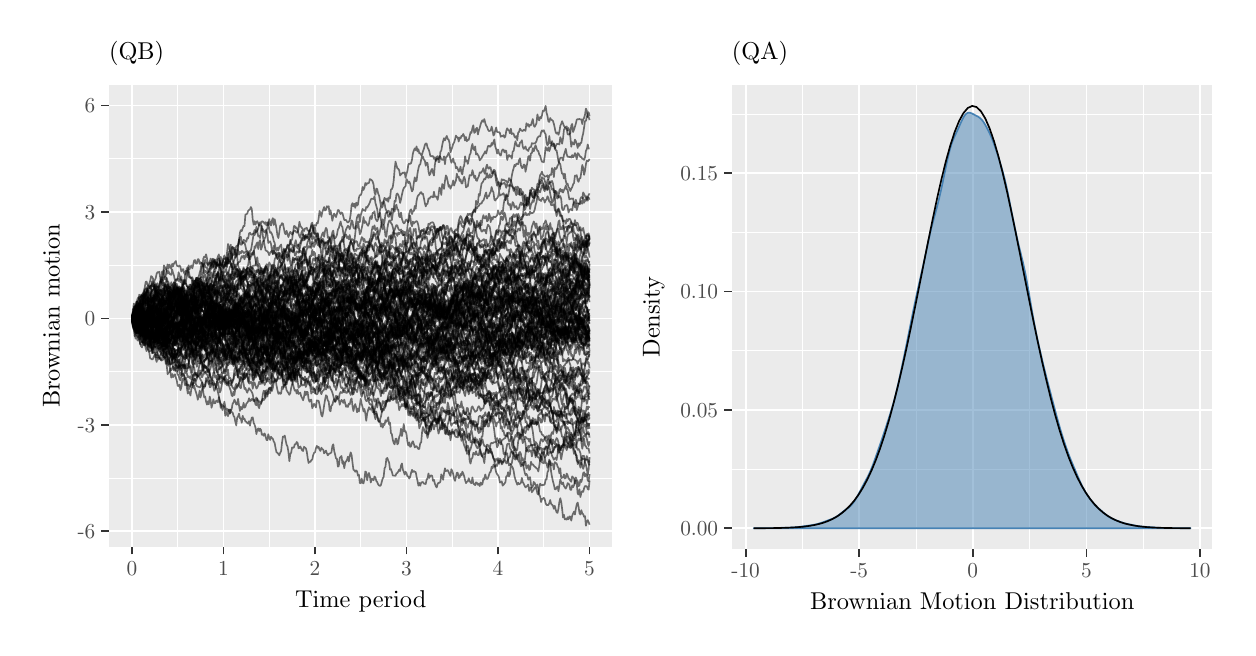
\begin{tikzpicture}[x=1pt,y=1pt]
\definecolor{fillColor}{RGB}{255,255,255}
\path[use as bounding box,fill=fillColor,fill opacity=0.00] (0,0) rectangle (433.62,216.81);
\begin{scope}
\path[clip] (  0.00,  0.00) rectangle (216.81,216.81);
\definecolor{drawColor}{RGB}{255,255,255}
\definecolor{fillColor}{RGB}{255,255,255}

\path[draw=drawColor,line width= 0.6pt,line join=round,line cap=round,fill=fillColor] (  0.00,  0.00) rectangle (216.81,216.81);
\end{scope}
\begin{scope}
\path[clip] ( 29.40, 29.26) rectangle (211.31,196.15);
\definecolor{fillColor}{gray}{0.92}

\path[fill=fillColor] ( 29.40, 29.26) rectangle (211.31,196.15);
\definecolor{drawColor}{RGB}{255,255,255}

\path[draw=drawColor,line width= 0.3pt,line join=round] ( 29.40, 54.09) --
	(211.31, 54.09);

\path[draw=drawColor,line width= 0.3pt,line join=round] ( 29.40, 92.54) --
	(211.31, 92.54);

\path[draw=drawColor,line width= 0.3pt,line join=round] ( 29.40,130.99) --
	(211.31,130.99);

\path[draw=drawColor,line width= 0.3pt,line join=round] ( 29.40,169.44) --
	(211.31,169.44);

\path[draw=drawColor,line width= 0.3pt,line join=round] ( 54.20, 29.26) --
	( 54.20,196.15);

\path[draw=drawColor,line width= 0.3pt,line join=round] ( 87.28, 29.26) --
	( 87.28,196.15);

\path[draw=drawColor,line width= 0.3pt,line join=round] (120.35, 29.26) --
	(120.35,196.15);

\path[draw=drawColor,line width= 0.3pt,line join=round] (153.43, 29.26) --
	(153.43,196.15);

\path[draw=drawColor,line width= 0.3pt,line join=round] (186.50, 29.26) --
	(186.50,196.15);

\path[draw=drawColor,line width= 0.6pt,line join=round] ( 29.40, 34.87) --
	(211.31, 34.87);

\path[draw=drawColor,line width= 0.6pt,line join=round] ( 29.40, 73.32) --
	(211.31, 73.32);

\path[draw=drawColor,line width= 0.6pt,line join=round] ( 29.40,111.77) --
	(211.31,111.77);

\path[draw=drawColor,line width= 0.6pt,line join=round] ( 29.40,150.22) --
	(211.31,150.22);

\path[draw=drawColor,line width= 0.6pt,line join=round] ( 29.40,188.67) --
	(211.31,188.67);

\path[draw=drawColor,line width= 0.6pt,line join=round] ( 37.67, 29.26) --
	( 37.67,196.15);

\path[draw=drawColor,line width= 0.6pt,line join=round] ( 70.74, 29.26) --
	( 70.74,196.15);

\path[draw=drawColor,line width= 0.6pt,line join=round] (103.82, 29.26) --
	(103.82,196.15);

\path[draw=drawColor,line width= 0.6pt,line join=round] (136.89, 29.26) --
	(136.89,196.15);

\path[draw=drawColor,line width= 0.6pt,line join=round] (169.97, 29.26) --
	(169.97,196.15);

\path[draw=drawColor,line width= 0.6pt,line join=round] (203.04, 29.26) --
	(203.04,196.15);
\definecolor{drawColor}{RGB}{0,0,0}

\path[draw=drawColor,draw opacity=0.55,line width= 0.6pt,line join=round] ( 37.67,111.77) --
	( 38.00,110.96) --
	( 38.33,111.20) --
	( 38.66,110.13) --
	( 38.99,112.17) --
	( 39.32,112.60) --
	( 39.65,111.54) --
	( 39.98,112.17) --
	( 40.31,113.11) --
	( 40.64,113.85) --
	( 40.97,113.46) --
	( 41.30,115.40) --
	( 41.64,115.90) --
	( 41.97,115.10) --
	( 42.30,112.26) --
	( 42.63,113.71) --
	( 42.96,113.65) --
	( 43.29,113.63) --
	( 43.62,114.84) --
	( 43.95,115.89) --
	( 44.28,116.65) --
	( 44.61,117.83) --
	( 44.94,118.83) --
	( 45.27,118.93) --
	( 45.60,116.38) --
	( 45.94,117.17) --
	( 46.27,117.10) --
	( 46.60,116.90) --
	( 46.93,115.01) --
	( 47.26,114.40) --
	( 47.59,114.94) --
	( 47.92,116.68) --
	( 48.25,116.55) --
	( 48.58,117.04) --
	( 48.91,116.98) --
	( 49.24,115.21) --
	( 49.57,114.68) --
	( 49.90,114.17) --
	( 50.24,114.10) --
	( 50.57,115.51) --
	( 50.90,116.48) --
	( 51.23,116.27) --
	( 51.56,115.95) --
	( 51.89,116.84) --
	( 52.22,117.56) --
	( 52.55,116.67) --
	( 52.88,115.77) --
	( 53.21,116.23) --
	( 53.54,117.22) --
	( 53.87,117.07) --
	( 54.20,118.20) --
	( 54.53,118.71) --
	( 54.87,117.93) --
	( 55.20,118.37) --
	( 55.53,116.92) --
	( 55.86,118.76) --
	( 56.19,121.29) --
	( 56.52,120.82) --
	( 56.85,119.49) --
	( 57.18,120.22) --
	( 57.51,120.04) --
	( 57.84,123.12) --
	( 58.17,123.07) --
	( 58.50,123.95) --
	( 58.83,123.99) --
	( 59.17,123.04) --
	( 59.50,123.28) --
	( 59.83,120.97) --
	( 60.16,122.84) --
	( 60.49,123.04) --
	( 60.82,125.83) --
	( 61.15,126.44) --
	( 61.48,125.53) --
	( 61.81,126.31) --
	( 62.14,125.11) --
	( 62.47,123.50) --
	( 62.80,123.88) --
	( 63.13,123.31) --
	( 63.47,123.31) --
	( 63.80,123.41) --
	( 64.13,122.65) --
	( 64.46,121.92) --
	( 64.79,121.75) --
	( 65.12,123.26) --
	( 65.45,121.31) --
	( 65.78,122.07) --
	( 66.11,122.49) --
	( 66.44,123.86) --
	( 66.77,123.47) --
	( 67.10,123.94) --
	( 67.43,124.28) --
	( 67.76,123.59) --
	( 68.10,125.14) --
	( 68.43,126.62) --
	( 68.76,127.52) --
	( 69.09,129.55) --
	( 69.42,130.27) --
	( 69.75,128.63) --
	( 70.08,127.90) --
	( 70.41,126.33) --
	( 70.74,125.72) --
	( 71.07,124.93) --
	( 71.40,124.98) --
	( 71.73,123.81) --
	( 72.06,124.02) --
	( 72.40,123.18) --
	( 72.73,125.44) --
	( 73.06,126.36) --
	( 73.39,127.53) --
	( 73.72,128.02) --
	( 74.05,130.18) --
	( 74.38,129.36) --
	( 74.71,128.77) --
	( 75.04,130.61) --
	( 75.37,129.77) --
	( 75.70,129.51) --
	( 76.03,129.00) --
	( 76.36,128.59) --
	( 76.70,128.23) --
	( 77.03,128.87) --
	( 77.36,128.64) --
	( 77.69,127.99) --
	( 78.02,129.71) --
	( 78.35,129.44) --
	( 78.68,129.21) --
	( 79.01,129.08) --
	( 79.34,129.99) --
	( 79.67,129.90) --
	( 80.00,129.85) --
	( 80.33,128.98) --
	( 80.66,128.56) --
	( 80.99,128.64) --
	( 81.33,127.88) --
	( 81.66,128.57) --
	( 81.99,126.62) --
	( 82.32,127.01) --
	( 82.65,125.04) --
	( 82.98,124.66) --
	( 83.31,123.98) --
	( 83.64,123.14) --
	( 83.97,123.07) --
	( 84.30,120.62) --
	( 84.63,122.13) --
	( 84.96,119.99) --
	( 85.29,119.40) --
	( 85.63,117.97) --
	( 85.96,117.00) --
	( 86.29,119.68) --
	( 86.62,119.70) --
	( 86.95,118.05) --
	( 87.28,115.95) --
	( 87.61,116.53) --
	( 87.94,116.50) --
	( 88.27,116.10) --
	( 88.60,114.91) --
	( 88.93,113.00) --
	( 89.26,111.62) --
	( 89.59,112.90) --
	( 89.93,112.11) --
	( 90.26,110.33) --
	( 90.59,112.73) --
	( 90.92,113.27) --
	( 91.25,112.97) --
	( 91.58,114.32) --
	( 91.91,115.46) --
	( 92.24,114.67) --
	( 92.57,117.49) --
	( 92.90,117.17) --
	( 93.23,115.34) --
	( 93.56,115.16) --
	( 93.89,115.42) --
	( 94.22,118.38) --
	( 94.56,118.52) --
	( 94.89,119.10) --
	( 95.22,119.00) --
	( 95.55,118.57) --
	( 95.88,118.53) --
	( 96.21,119.54) --
	( 96.54,122.20) --
	( 96.87,123.52) --
	( 97.20,125.06) --
	( 97.53,123.49) --
	( 97.86,124.75) --
	( 98.19,125.03) --
	( 98.52,123.15) --
	( 98.86,123.82) --
	( 99.19,123.61) --
	( 99.52,125.49) --
	( 99.85,124.51) --
	(100.18,123.96) --
	(100.51,122.77) --
	(100.84,122.54) --
	(101.17,123.06) --
	(101.50,122.12) --
	(101.83,123.18) --
	(102.16,121.64) --
	(102.49,120.29) --
	(102.82,122.14) --
	(103.15,120.84) --
	(103.49,121.37) --
	(103.82,120.88) --
	(104.15,121.40) --
	(104.48,123.57) --
	(104.81,125.60) --
	(105.14,125.18) --
	(105.47,122.25) --
	(105.80,125.45) --
	(106.13,126.30) --
	(106.46,127.00) --
	(106.79,126.98) --
	(107.12,127.63) --
	(107.45,127.42) --
	(107.79,127.96) --
	(108.12,127.45) --
	(108.45,125.69) --
	(108.78,126.96) --
	(109.11,128.91) --
	(109.44,128.51) --
	(109.77,126.90) --
	(110.10,127.73) --
	(110.43,127.67) --
	(110.76,125.45) --
	(111.09,125.45) --
	(111.42,124.64) --
	(111.75,124.21) --
	(112.09,122.72) --
	(112.42,125.04) --
	(112.75,124.61) --
	(113.08,122.55) --
	(113.41,122.81) --
	(113.74,123.14) --
	(114.07,121.88) --
	(114.40,118.18) --
	(114.73,117.36) --
	(115.06,118.09) --
	(115.39,118.01) --
	(115.72,117.89) --
	(116.05,118.60) --
	(116.38,117.08) --
	(116.72,118.49) --
	(117.05,118.48) --
	(117.38,119.39) --
	(117.71,120.71) --
	(118.04,121.00) --
	(118.37,119.87) --
	(118.70,121.37) --
	(119.03,118.80) --
	(119.36,118.10) --
	(119.69,117.78) --
	(120.02,117.56) --
	(120.35,118.87) --
	(120.68,119.05) --
	(121.02,119.57) --
	(121.35,119.48) --
	(121.68,119.16) --
	(122.01,120.05) --
	(122.34,121.52) --
	(122.67,118.44) --
	(123.00,119.17) --
	(123.33,119.66) --
	(123.66,119.11) --
	(123.99,120.33) --
	(124.32,119.83) --
	(124.65,119.47) --
	(124.98,120.56) --
	(125.32,122.77) --
	(125.65,123.11) --
	(125.98,122.57) --
	(126.31,121.05) --
	(126.64,120.63) --
	(126.97,119.42) --
	(127.30,119.09) --
	(127.63,119.59) --
	(127.96,118.50) --
	(128.29,121.90) --
	(128.62,122.10) --
	(128.95,123.55) --
	(129.28,120.61) --
	(129.61,121.56) --
	(129.95,119.88) --
	(130.28,121.05) --
	(130.61,121.56) --
	(130.94,121.04) --
	(131.27,122.74) --
	(131.60,121.84) --
	(131.93,121.10) --
	(132.26,119.81) --
	(132.59,118.96) --
	(132.92,120.17) --
	(133.25,120.72) --
	(133.58,122.01) --
	(133.91,121.51) --
	(134.25,122.00) --
	(134.58,122.31) --
	(134.91,120.48) --
	(135.24,122.76) --
	(135.57,122.93) --
	(135.90,123.91) --
	(136.23,125.14) --
	(136.56,125.07) --
	(136.89,124.68) --
	(137.22,125.83) --
	(137.55,124.48) --
	(137.88,127.01) --
	(138.21,126.52) --
	(138.55,128.64) --
	(138.88,130.58) --
	(139.21,130.68) --
	(139.54,131.41) --
	(139.87,130.10) --
	(140.20,130.51) --
	(140.53,131.85) --
	(140.86,131.98) --
	(141.19,131.39) --
	(141.52,130.55) --
	(141.85,130.51) --
	(142.18,131.88) --
	(142.51,131.26) --
	(142.84,131.10) --
	(143.18,129.44) --
	(143.51,130.08) --
	(143.84,131.75) --
	(144.17,133.67) --
	(144.50,134.72) --
	(144.83,132.32) --
	(145.16,132.94) --
	(145.49,133.52) --
	(145.82,133.07) --
	(146.15,133.29) --
	(146.48,132.18) --
	(146.81,133.05) --
	(147.14,132.63) --
	(147.48,130.62) --
	(147.81,130.15) --
	(148.14,131.90) --
	(148.47,131.47) --
	(148.80,132.41) --
	(149.13,133.62) --
	(149.46,133.63) --
	(149.79,133.18) --
	(150.12,132.50) --
	(150.45,133.45) --
	(150.78,132.08) --
	(151.11,132.40) --
	(151.44,132.03) --
	(151.78,129.12) --
	(152.11,127.32) --
	(152.44,128.49) --
	(152.77,128.25) --
	(153.10,129.28) --
	(153.43,131.70) --
	(153.76,133.58) --
	(154.09,134.45) --
	(154.42,134.94) --
	(154.75,134.69) --
	(155.08,136.72) --
	(155.41,137.48) --
	(155.74,135.98) --
	(156.07,135.78) --
	(156.41,133.32) --
	(156.74,133.07) --
	(157.07,129.74) --
	(157.40,131.43) --
	(157.73,130.61) --
	(158.06,130.06) --
	(158.39,129.84) --
	(158.72,130.63) --
	(159.05,131.50) --
	(159.38,132.23) --
	(159.71,131.49) --
	(160.04,129.75) --
	(160.37,129.25) --
	(160.71,129.60) --
	(161.04,128.55) --
	(161.37,128.46) --
	(161.70,126.96) --
	(162.03,126.95) --
	(162.36,127.12) --
	(162.69,126.93) --
	(163.02,126.72) --
	(163.35,128.98) --
	(163.68,129.96) --
	(164.01,131.38) --
	(164.34,130.20) --
	(164.67,130.41) --
	(165.01,131.89) --
	(165.34,131.82) --
	(165.67,129.09) --
	(166.00,129.53) --
	(166.33,127.09) --
	(166.66,126.05) --
	(166.99,127.75) --
	(167.32,128.54) --
	(167.65,129.94) --
	(167.98,130.33) --
	(168.31,130.19) --
	(168.64,129.00) --
	(168.97,131.04) --
	(169.30,131.10) --
	(169.64,130.19) --
	(169.97,131.29) --
	(170.30,132.67) --
	(170.63,135.10) --
	(170.96,134.33) --
	(171.29,133.83) --
	(171.62,133.29) --
	(171.95,132.81) --
	(172.28,132.34) --
	(172.61,131.96) --
	(172.94,133.81) --
	(173.27,132.92) --
	(173.60,132.42) --
	(173.94,133.26) --
	(174.27,134.70) --
	(174.60,133.71) --
	(174.93,133.06) --
	(175.26,133.73) --
	(175.59,135.03) --
	(175.92,134.71) --
	(176.25,132.88) --
	(176.58,135.07) --
	(176.91,136.91) --
	(177.24,136.00) --
	(177.57,135.91) --
	(177.90,133.66) --
	(178.24,134.39) --
	(178.57,136.46) --
	(178.90,134.36) --
	(179.23,133.36) --
	(179.56,132.54) --
	(179.89,131.66) --
	(180.22,129.06) --
	(180.55,129.70) --
	(180.88,127.74) --
	(181.21,127.70) --
	(181.54,128.46) --
	(181.87,128.21) --
	(182.20,129.35) --
	(182.53,129.32) --
	(182.87,128.49) --
	(183.20,129.32) --
	(183.53,128.76) --
	(183.86,131.03) --
	(184.19,131.01) --
	(184.52,132.10) --
	(184.85,132.37) --
	(185.18,128.51) --
	(185.51,126.76) --
	(185.84,126.22) --
	(186.17,126.52) --
	(186.50,123.52) --
	(186.83,124.75) --
	(187.17,123.98) --
	(187.50,123.01) --
	(187.83,121.02) --
	(188.16,119.15) --
	(188.49,119.23) --
	(188.82,119.88) --
	(189.15,117.19) --
	(189.48,115.90) --
	(189.81,116.59) --
	(190.14,116.01) --
	(190.47,118.78) --
	(190.80,120.38) --
	(191.13,121.14) --
	(191.47,121.15) --
	(191.80,121.51) --
	(192.13,120.60) --
	(192.46,121.41) --
	(192.79,123.31) --
	(193.12,124.69) --
	(193.45,123.65) --
	(193.78,121.58) --
	(194.11,121.44) --
	(194.44,122.00) --
	(194.77,123.73) --
	(195.10,122.04) --
	(195.43,122.51) --
	(195.76,122.81) --
	(196.10,124.34) --
	(196.43,124.30) --
	(196.76,123.85) --
	(197.09,122.38) --
	(197.42,121.71) --
	(197.75,121.25) --
	(198.08,124.26) --
	(198.41,127.40) --
	(198.74,127.18) --
	(199.07,125.85) --
	(199.40,123.32) --
	(199.73,123.98) --
	(200.06,122.58) --
	(200.40,125.51) --
	(200.73,124.37) --
	(201.06,124.51) --
	(201.39,129.40) --
	(201.72,127.98) --
	(202.05,128.37) --
	(202.38,126.95) --
	(202.71,127.40) --
	(203.04,126.28);

\path[draw=drawColor,draw opacity=0.55,line width= 0.6pt,line join=round] ( 37.67,111.77) --
	( 38.00,113.76) --
	( 38.33,112.83) --
	( 38.66,110.90) --
	( 38.99,110.17) --
	( 39.32,107.48) --
	( 39.65,108.16) --
	( 39.98,110.23) --
	( 40.31,111.75) --
	( 40.64,114.15) --
	( 40.97,113.57) --
	( 41.30,114.43) --
	( 41.64,112.78) --
	( 41.97,112.28) --
	( 42.30,112.12) --
	( 42.63,110.90) --
	( 42.96,111.43) --
	( 43.29,111.30) --
	( 43.62,110.91) --
	( 43.95,111.31) --
	( 44.28,111.64) --
	( 44.61,111.86) --
	( 44.94,110.48) --
	( 45.27,110.62) --
	( 45.60,109.06) --
	( 45.94,109.62) --
	( 46.27,106.78) --
	( 46.60,110.29) --
	( 46.93,110.63) --
	( 47.26,108.68) --
	( 47.59,108.68) --
	( 47.92,105.55) --
	( 48.25,105.93) --
	( 48.58,103.03) --
	( 48.91,102.49) --
	( 49.24,102.33) --
	( 49.57,101.84) --
	( 49.90,100.77) --
	( 50.24,101.64) --
	( 50.57,102.69) --
	( 50.90,100.62) --
	( 51.23,100.50) --
	( 51.56, 99.02) --
	( 51.89, 98.08) --
	( 52.22, 99.19) --
	( 52.55, 97.10) --
	( 52.88, 97.90) --
	( 53.21, 97.09) --
	( 53.54, 97.19) --
	( 53.87, 98.97) --
	( 54.20, 99.13) --
	( 54.53, 98.13) --
	( 54.87, 99.29) --
	( 55.20, 98.46) --
	( 55.53,100.25) --
	( 55.86,101.74) --
	( 56.19,102.30) --
	( 56.52,102.67) --
	( 56.85,102.32) --
	( 57.18,100.00) --
	( 57.51,101.66) --
	( 57.84,101.75) --
	( 58.17,100.77) --
	( 58.50,100.14) --
	( 58.83, 98.87) --
	( 59.17, 98.91) --
	( 59.50, 97.88) --
	( 59.83, 94.34) --
	( 60.16, 94.12) --
	( 60.49, 91.80) --
	( 60.82, 91.51) --
	( 61.15, 90.36) --
	( 61.48, 91.14) --
	( 61.81, 91.15) --
	( 62.14, 92.97) --
	( 62.47, 92.83) --
	( 62.80, 90.57) --
	( 63.13, 90.57) --
	( 63.47, 91.91) --
	( 63.80, 91.70) --
	( 64.13, 92.39) --
	( 64.46, 92.33) --
	( 64.79, 92.73) --
	( 65.12, 93.34) --
	( 65.45, 92.95) --
	( 65.78, 91.85) --
	( 66.11, 89.83) --
	( 66.44, 88.98) --
	( 66.77, 89.70) --
	( 67.10, 92.11) --
	( 67.43, 92.28) --
	( 67.76, 90.33) --
	( 68.10, 91.12) --
	( 68.43, 89.64) --
	( 68.76, 89.44) --
	( 69.09, 89.95) --
	( 69.42, 90.62) --
	( 69.75, 90.88) --
	( 70.08, 90.46) --
	( 70.41, 89.46) --
	( 70.74, 90.72) --
	( 71.07, 89.92) --
	( 71.40, 88.09) --
	( 71.73, 88.25) --
	( 72.06, 87.51) --
	( 72.40, 87.64) --
	( 72.73, 89.08) --
	( 73.06, 89.19) --
	( 73.39, 89.37) --
	( 73.72, 88.54) --
	( 74.05, 89.60) --
	( 74.38, 89.56) --
	( 74.71, 91.60) --
	( 75.04, 91.22) --
	( 75.37, 92.92) --
	( 75.70, 91.37) --
	( 76.03, 90.29) --
	( 76.36, 90.71) --
	( 76.70, 88.84) --
	( 77.03, 90.40) --
	( 77.36, 90.18) --
	( 77.69, 89.76) --
	( 78.02, 90.35) --
	( 78.35, 89.81) --
	( 78.68, 90.53) --
	( 79.01, 91.09) --
	( 79.34, 91.85) --
	( 79.67, 92.73) --
	( 80.00, 91.48) --
	( 80.33, 93.42) --
	( 80.66, 93.52) --
	( 80.99, 93.13) --
	( 81.33, 93.31) --
	( 81.66, 91.31) --
	( 81.99, 91.00) --
	( 82.32, 90.33) --
	( 82.65, 93.51) --
	( 82.98, 95.73) --
	( 83.31, 96.23) --
	( 83.64, 95.72) --
	( 83.97, 96.69) --
	( 84.30, 96.52) --
	( 84.63, 96.97) --
	( 84.96, 95.37) --
	( 85.29, 98.55) --
	( 85.63,100.43) --
	( 85.96,100.69) --
	( 86.29,100.63) --
	( 86.62, 99.52) --
	( 86.95, 99.49) --
	( 87.28, 99.31) --
	( 87.61, 99.36) --
	( 87.94, 99.98) --
	( 88.27,100.65) --
	( 88.60,103.20) --
	( 88.93,103.66) --
	( 89.26,104.02) --
	( 89.59,103.49) --
	( 89.93,103.73) --
	( 90.26,102.47) --
	( 90.59,101.72) --
	( 90.92,102.90) --
	( 91.25,102.26) --
	( 91.58,102.34) --
	( 91.91,101.87) --
	( 92.24,102.02) --
	( 92.57,101.18) --
	( 92.90,102.39) --
	( 93.23,102.70) --
	( 93.56,102.92) --
	( 93.89,101.60) --
	( 94.22,102.28) --
	( 94.56,101.88) --
	( 94.89,104.79) --
	( 95.22,107.37) --
	( 95.55,107.70) --
	( 95.88,106.33) --
	( 96.21,107.33) --
	( 96.54,108.06) --
	( 96.87,107.28) --
	( 97.20,109.21) --
	( 97.53,108.65) --
	( 97.86,107.42) --
	( 98.19,108.63) --
	( 98.52,108.95) --
	( 98.86,107.26) --
	( 99.19,106.45) --
	( 99.52,105.58) --
	( 99.85,104.38) --
	(100.18,105.44) --
	(100.51,105.37) --
	(100.84,108.18) --
	(101.17,108.97) --
	(101.50,110.67) --
	(101.83,112.02) --
	(102.16,111.87) --
	(102.49,112.16) --
	(102.82,114.03) --
	(103.15,114.26) --
	(103.49,113.55) --
	(103.82,114.30) --
	(104.15,114.24) --
	(104.48,114.97) --
	(104.81,115.86) --
	(105.14,117.45) --
	(105.47,117.36) --
	(105.80,117.06) --
	(106.13,119.07) --
	(106.46,119.57) --
	(106.79,118.78) --
	(107.12,118.59) --
	(107.45,118.14) --
	(107.79,117.45) --
	(108.12,115.37) --
	(108.45,116.65) --
	(108.78,114.52) --
	(109.11,115.43) --
	(109.44,113.22) --
	(109.77,110.73) --
	(110.10,109.54) --
	(110.43,110.07) --
	(110.76,111.56) --
	(111.09,112.79) --
	(111.42,110.86) --
	(111.75,111.65) --
	(112.09,111.76) --
	(112.42,112.14) --
	(112.75,110.62) --
	(113.08,109.20) --
	(113.41,110.91) --
	(113.74,111.12) --
	(114.07,112.14) --
	(114.40,112.17) --
	(114.73,111.85) --
	(115.06,108.76) --
	(115.39,110.38) --
	(115.72,112.85) --
	(116.05,114.95) --
	(116.38,115.34) --
	(116.72,117.28) --
	(117.05,118.52) --
	(117.38,119.04) --
	(117.71,120.34) --
	(118.04,120.29) --
	(118.37,117.84) --
	(118.70,119.03) --
	(119.03,120.22) --
	(119.36,121.63) --
	(119.69,119.53) --
	(120.02,118.57) --
	(120.35,118.38) --
	(120.68,120.77) --
	(121.02,119.99) --
	(121.35,118.91) --
	(121.68,121.95) --
	(122.01,121.97) --
	(122.34,122.02) --
	(122.67,121.03) --
	(123.00,122.22) --
	(123.33,124.06) --
	(123.66,122.55) --
	(123.99,122.75) --
	(124.32,123.78) --
	(124.65,125.24) --
	(124.98,124.59) --
	(125.32,121.29) --
	(125.65,121.04) --
	(125.98,121.48) --
	(126.31,122.51) --
	(126.64,120.61) --
	(126.97,119.91) --
	(127.30,119.43) --
	(127.63,118.78) --
	(127.96,120.18) --
	(128.29,118.50) --
	(128.62,117.66) --
	(128.95,116.14) --
	(129.28,114.25) --
	(129.61,115.63) --
	(129.95,114.87) --
	(130.28,115.31) --
	(130.61,114.00) --
	(130.94,115.61) --
	(131.27,112.94) --
	(131.60,113.24) --
	(131.93,112.58) --
	(132.26,113.45) --
	(132.59,112.04) --
	(132.92,113.45) --
	(133.25,112.37) --
	(133.58,110.93) --
	(133.91,111.96) --
	(134.25,113.35) --
	(134.58,113.85) --
	(134.91,113.26) --
	(135.24,112.99) --
	(135.57,112.77) --
	(135.90,110.89) --
	(136.23,111.02) --
	(136.56,111.20) --
	(136.89,110.34) --
	(137.22,108.87) --
	(137.55,110.38) --
	(137.88,109.77) --
	(138.21,111.88) --
	(138.55,111.46) --
	(138.88,111.65) --
	(139.21,112.62) --
	(139.54,113.81) --
	(139.87,115.34) --
	(140.20,115.64) --
	(140.53,116.49) --
	(140.86,118.34) --
	(141.19,118.79) --
	(141.52,120.74) --
	(141.85,121.12) --
	(142.18,119.93) --
	(142.51,120.65) --
	(142.84,118.73) --
	(143.18,119.38) --
	(143.51,117.83) --
	(143.84,117.41) --
	(144.17,118.28) --
	(144.50,117.33) --
	(144.83,115.46) --
	(145.16,115.33) --
	(145.49,114.57) --
	(145.82,116.03) --
	(146.15,114.62) --
	(146.48,112.83) --
	(146.81,111.85) --
	(147.14,113.69) --
	(147.48,114.80) --
	(147.81,113.85) --
	(148.14,111.87) --
	(148.47,112.37) --
	(148.80,110.50) --
	(149.13,110.31) --
	(149.46,109.44) --
	(149.79,108.93) --
	(150.12,109.44) --
	(150.45,110.22) --
	(150.78,110.59) --
	(151.11,108.51) --
	(151.44,109.33) --
	(151.78,108.85) --
	(152.11,110.27) --
	(152.44,110.77) --
	(152.77,110.20) --
	(153.10,112.83) --
	(153.43,113.41) --
	(153.76,112.07) --
	(154.09,112.00) --
	(154.42,110.71) --
	(154.75,108.96) --
	(155.08,109.26) --
	(155.41,109.57) --
	(155.74,110.60) --
	(156.07,112.53) --
	(156.41,113.08) --
	(156.74,113.09) --
	(157.07,113.20) --
	(157.40,114.31) --
	(157.73,113.07) --
	(158.06,111.92) --
	(158.39,110.62) --
	(158.72,111.80) --
	(159.05,112.67) --
	(159.38,110.59) --
	(159.71,111.52) --
	(160.04,110.03) --
	(160.37,110.24) --
	(160.71,111.59) --
	(161.04,110.59) --
	(161.37,111.31) --
	(161.70,110.90) --
	(162.03,112.46) --
	(162.36,113.29) --
	(162.69,114.04) --
	(163.02,111.80) --
	(163.35,111.22) --
	(163.68,108.85) --
	(164.01,108.58) --
	(164.34,108.28) --
	(164.67,107.81) --
	(165.01,107.37) --
	(165.34,106.96) --
	(165.67,105.32) --
	(166.00,104.40) --
	(166.33,103.66) --
	(166.66,104.05) --
	(166.99,105.89) --
	(167.32,105.11) --
	(167.65,102.48) --
	(167.98,102.04) --
	(168.31,100.77) --
	(168.64,101.42) --
	(168.97,101.32) --
	(169.30,101.97) --
	(169.64,103.71) --
	(169.97,103.40) --
	(170.30,100.69) --
	(170.63, 99.84) --
	(170.96,100.25) --
	(171.29,100.12) --
	(171.62,100.07) --
	(171.95, 98.86) --
	(172.28, 98.16) --
	(172.61, 98.91) --
	(172.94,101.95) --
	(173.27,103.21) --
	(173.60,105.93) --
	(173.94,105.19) --
	(174.27,104.01) --
	(174.60,103.86) --
	(174.93,105.02) --
	(175.26,106.65) --
	(175.59,104.12) --
	(175.92,103.34) --
	(176.25,101.32) --
	(176.58,102.76) --
	(176.91,105.01) --
	(177.24,106.53) --
	(177.57,106.63) --
	(177.90,104.61) --
	(178.24,104.02) --
	(178.57,102.22) --
	(178.90,104.10) --
	(179.23,102.50) --
	(179.56,103.34) --
	(179.89,102.92) --
	(180.22,101.10) --
	(180.55,100.80) --
	(180.88,103.44) --
	(181.21,105.62) --
	(181.54,103.39) --
	(181.87,101.76) --
	(182.20,100.50) --
	(182.53,101.87) --
	(182.87,101.30) --
	(183.20,101.13) --
	(183.53,102.08) --
	(183.86,101.09) --
	(184.19,101.57) --
	(184.52,102.03) --
	(184.85,101.90) --
	(185.18,103.71) --
	(185.51,103.06) --
	(185.84,103.02) --
	(186.17,101.84) --
	(186.50,101.32) --
	(186.83, 99.38) --
	(187.17, 99.71) --
	(187.50,101.71) --
	(187.83,100.00) --
	(188.16, 98.80) --
	(188.49, 98.74) --
	(188.82, 96.41) --
	(189.15, 95.60) --
	(189.48, 95.12) --
	(189.81, 93.71) --
	(190.14, 93.42) --
	(190.47, 94.49) --
	(190.80, 94.79) --
	(191.13, 94.41) --
	(191.47, 94.00) --
	(191.80, 91.78) --
	(192.13, 91.13) --
	(192.46, 91.32) --
	(192.79, 91.79) --
	(193.12, 90.96) --
	(193.45, 92.28) --
	(193.78, 93.82) --
	(194.11, 93.91) --
	(194.44, 92.28) --
	(194.77, 90.95) --
	(195.10, 91.37) --
	(195.43, 91.93) --
	(195.76, 92.38) --
	(196.10, 93.99) --
	(196.43, 93.96) --
	(196.76, 92.59) --
	(197.09, 94.14) --
	(197.42, 93.01) --
	(197.75, 93.17) --
	(198.08, 93.86) --
	(198.41, 93.69) --
	(198.74, 94.21) --
	(199.07, 94.17) --
	(199.40, 92.72) --
	(199.73, 91.88) --
	(200.06, 91.01) --
	(200.40, 91.94) --
	(200.73, 93.41) --
	(201.06, 91.11) --
	(201.39, 89.31) --
	(201.72, 89.52) --
	(202.05, 90.78) --
	(202.38, 89.89) --
	(202.71, 89.89) --
	(203.04, 90.11);

\path[draw=drawColor,draw opacity=0.55,line width= 0.6pt,line join=round] ( 37.67,111.77) --
	( 38.00,112.47) --
	( 38.33,112.25) --
	( 38.66,112.79) --
	( 38.99,110.91) --
	( 39.32,111.24) --
	( 39.65,111.42) --
	( 39.98,109.06) --
	( 40.31,108.25) --
	( 40.64,107.69) --
	( 40.97,107.01) --
	( 41.30,109.06) --
	( 41.64,109.91) --
	( 41.97,110.95) --
	( 42.30,109.83) --
	( 42.63,108.44) --
	( 42.96,107.44) --
	( 43.29,107.95) --
	( 43.62,107.04) --
	( 43.95,107.43) --
	( 44.28,106.35) --
	( 44.61,108.60) --
	( 44.94,107.50) --
	( 45.27,108.33) --
	( 45.60,106.34) --
	( 45.94,105.01) --
	( 46.27,104.39) --
	( 46.60,105.07) --
	( 46.93,106.39) --
	( 47.26,103.80) --
	( 47.59,105.34) --
	( 47.92,106.12) --
	( 48.25,107.10) --
	( 48.58,105.90) --
	( 48.91,107.35) --
	( 49.24,106.21) --
	( 49.57,105.21) --
	( 49.90,104.26) --
	( 50.24,102.79) --
	( 50.57,104.00) --
	( 50.90,103.32) --
	( 51.23,105.73) --
	( 51.56,106.34) --
	( 51.89,107.06) --
	( 52.22,107.52) --
	( 52.55,108.42) --
	( 52.88,108.95) --
	( 53.21,107.95) --
	( 53.54,108.33) --
	( 53.87,110.00) --
	( 54.20,112.31) --
	( 54.53,112.97) --
	( 54.87,114.84) --
	( 55.20,112.83) --
	( 55.53,111.39) --
	( 55.86,110.63) --
	( 56.19,111.31) --
	( 56.52,113.67) --
	( 56.85,114.11) --
	( 57.18,112.97) --
	( 57.51,112.41) --
	( 57.84,111.69) --
	( 58.17,111.60) --
	( 58.50,110.79) --
	( 58.83,109.91) --
	( 59.17,109.55) --
	( 59.50,108.18) --
	( 59.83,108.13) --
	( 60.16,110.93) --
	( 60.49,112.54) --
	( 60.82,113.91) --
	( 61.15,112.97) --
	( 61.48,111.73) --
	( 61.81,109.64) --
	( 62.14,110.78) --
	( 62.47,108.94) --
	( 62.80,108.00) --
	( 63.13,110.03) --
	( 63.47,109.70) --
	( 63.80,110.21) --
	( 64.13,112.00) --
	( 64.46,112.14) --
	( 64.79,112.51) --
	( 65.12,112.91) --
	( 65.45,112.31) --
	( 65.78,108.80) --
	( 66.11,109.61) --
	( 66.44,109.85) --
	( 66.77,110.89) --
	( 67.10,111.71) --
	( 67.43,109.49) --
	( 67.76,109.17) --
	( 68.10,109.95) --
	( 68.43,110.14) --
	( 68.76,109.44) --
	( 69.09,110.32) --
	( 69.42,109.70) --
	( 69.75,110.08) --
	( 70.08,109.00) --
	( 70.41,110.08) --
	( 70.74,110.50) --
	( 71.07,112.61) --
	( 71.40,111.94) --
	( 71.73,109.26) --
	( 72.06,108.20) --
	( 72.40,106.42) --
	( 72.73,106.21) --
	( 73.06,108.05) --
	( 73.39,110.44) --
	( 73.72,112.17) --
	( 74.05,110.71) --
	( 74.38,110.87) --
	( 74.71,109.07) --
	( 75.04,108.20) --
	( 75.37,108.54) --
	( 75.70,108.80) --
	( 76.03,110.06) --
	( 76.36,110.15) --
	( 76.70,109.98) --
	( 77.03,109.83) --
	( 77.36,109.53) --
	( 77.69,108.65) --
	( 78.02,108.95) --
	( 78.35,107.14) --
	( 78.68,108.82) --
	( 79.01,106.21) --
	( 79.34,105.66) --
	( 79.67,106.54) --
	( 80.00,105.87) --
	( 80.33,105.70) --
	( 80.66,105.51) --
	( 80.99,105.11) --
	( 81.33,102.77) --
	( 81.66,103.47) --
	( 81.99,105.22) --
	( 82.32,105.52) --
	( 82.65,105.57) --
	( 82.98,104.83) --
	( 83.31,106.62) --
	( 83.64,107.66) --
	( 83.97,109.50) --
	( 84.30,108.58) --
	( 84.63,109.27) --
	( 84.96,105.43) --
	( 85.29,108.11) --
	( 85.63,108.01) --
	( 85.96,106.77) --
	( 86.29,107.12) --
	( 86.62,107.24) --
	( 86.95,107.67) --
	( 87.28,108.82) --
	( 87.61,107.68) --
	( 87.94,107.37) --
	( 88.27,107.74) --
	( 88.60,108.39) --
	( 88.93,107.79) --
	( 89.26,108.45) --
	( 89.59,109.28) --
	( 89.93,108.20) --
	( 90.26,109.20) --
	( 90.59,108.14) --
	( 90.92,104.38) --
	( 91.25,101.04) --
	( 91.58, 97.13) --
	( 91.91, 96.76) --
	( 92.24, 97.26) --
	( 92.57, 98.36) --
	( 92.90, 97.42) --
	( 93.23, 96.91) --
	( 93.56, 95.51) --
	( 93.89, 94.22) --
	( 94.22, 95.33) --
	( 94.56, 96.59) --
	( 94.89, 97.07) --
	( 95.22, 97.38) --
	( 95.55, 97.32) --
	( 95.88, 95.15) --
	( 96.21, 93.52) --
	( 96.54, 95.68) --
	( 96.87, 96.07) --
	( 97.20, 95.28) --
	( 97.53, 94.44) --
	( 97.86, 94.51) --
	( 98.19, 95.59) --
	( 98.52, 95.94) --
	( 98.86, 95.33) --
	( 99.19, 94.40) --
	( 99.52, 93.85) --
	( 99.85, 95.05) --
	(100.18, 95.68) --
	(100.51, 95.86) --
	(100.84, 94.26) --
	(101.17, 92.40) --
	(101.50, 92.84) --
	(101.83, 92.75) --
	(102.16, 93.07) --
	(102.49, 94.12) --
	(102.82, 91.97) --
	(103.15, 93.55) --
	(103.49, 94.89) --
	(103.82, 95.89) --
	(104.15, 96.52) --
	(104.48, 95.78) --
	(104.81, 96.69) --
	(105.14, 95.56) --
	(105.47, 94.79) --
	(105.80, 93.73) --
	(106.13, 95.94) --
	(106.46, 99.38) --
	(106.79, 99.77) --
	(107.12, 98.66) --
	(107.45,100.63) --
	(107.79,100.23) --
	(108.12,101.65) --
	(108.45,102.38) --
	(108.78,103.57) --
	(109.11,104.75) --
	(109.44,106.22) --
	(109.77,106.69) --
	(110.10,105.75) --
	(110.43,106.91) --
	(110.76,106.99) --
	(111.09,104.35) --
	(111.42,103.75) --
	(111.75,102.50) --
	(112.09,103.09) --
	(112.42,103.66) --
	(112.75,104.77) --
	(113.08,105.06) --
	(113.41,102.72) --
	(113.74,103.47) --
	(114.07,102.65) --
	(114.40,100.92) --
	(114.73,101.54) --
	(115.06, 98.65) --
	(115.39, 99.09) --
	(115.72, 98.45) --
	(116.05, 98.52) --
	(116.38, 98.50) --
	(116.72, 98.84) --
	(117.05, 98.07) --
	(117.38, 97.06) --
	(117.71, 96.84) --
	(118.04, 96.72) --
	(118.37, 96.58) --
	(118.70, 99.25) --
	(119.03, 98.64) --
	(119.36, 98.26) --
	(119.69, 99.35) --
	(120.02, 96.31) --
	(120.35, 97.04) --
	(120.68, 98.28) --
	(121.02, 98.06) --
	(121.35, 99.99) --
	(121.68,101.04) --
	(122.01, 99.98) --
	(122.34, 98.08) --
	(122.67, 97.30) --
	(123.00, 99.08) --
	(123.33, 99.64) --
	(123.66, 99.68) --
	(123.99,100.80) --
	(124.32,100.87) --
	(124.65,100.44) --
	(124.98,100.00) --
	(125.32, 99.67) --
	(125.65, 96.84) --
	(125.98, 94.88) --
	(126.31, 94.62) --
	(126.64, 92.79) --
	(126.97, 92.16) --
	(127.30, 91.75) --
	(127.63, 91.37) --
	(127.96, 89.05) --
	(128.29, 89.75) --
	(128.62, 89.37) --
	(128.95, 91.18) --
	(129.28, 91.15) --
	(129.61, 92.61) --
	(129.95, 91.91) --
	(130.28, 92.52) --
	(130.61, 94.94) --
	(130.94, 95.34) --
	(131.27, 95.88) --
	(131.60, 93.62) --
	(131.93, 93.79) --
	(132.26, 96.72) --
	(132.59, 97.71) --
	(132.92, 98.63) --
	(133.25, 97.98) --
	(133.58, 97.98) --
	(133.91, 96.60) --
	(134.25, 96.82) --
	(134.58, 96.84) --
	(134.91, 98.49) --
	(135.24, 97.18) --
	(135.57, 94.41) --
	(135.90, 94.64) --
	(136.23, 94.39) --
	(136.56, 95.04) --
	(136.89, 94.40) --
	(137.22, 94.81) --
	(137.55, 97.59) --
	(137.88, 98.44) --
	(138.21, 96.81) --
	(138.55, 98.87) --
	(138.88,100.87) --
	(139.21,102.55) --
	(139.54,103.44) --
	(139.87,103.36) --
	(140.20,102.74) --
	(140.53,101.76) --
	(140.86,103.31) --
	(141.19, 99.97) --
	(141.52, 98.16) --
	(141.85,101.29) --
	(142.18,100.75) --
	(142.51, 99.73) --
	(142.84,100.04) --
	(143.18, 99.41) --
	(143.51, 99.72) --
	(143.84, 99.38) --
	(144.17, 99.11) --
	(144.50,100.52) --
	(144.83, 99.93) --
	(145.16, 99.25) --
	(145.49, 98.66) --
	(145.82, 99.21) --
	(146.15, 98.62) --
	(146.48,100.02) --
	(146.81,100.05) --
	(147.14, 98.27) --
	(147.48, 97.97) --
	(147.81,100.57) --
	(148.14,102.56) --
	(148.47,101.15) --
	(148.80,100.01) --
	(149.13,101.89) --
	(149.46,101.05) --
	(149.79,100.01) --
	(150.12,100.89) --
	(150.45,102.66) --
	(150.78,102.68) --
	(151.11,101.20) --
	(151.44,101.63) --
	(151.78,102.16) --
	(152.11,102.20) --
	(152.44,100.56) --
	(152.77, 99.13) --
	(153.10, 99.36) --
	(153.43,100.86) --
	(153.76,100.42) --
	(154.09,102.29) --
	(154.42,102.25) --
	(154.75,102.20) --
	(155.08,104.34) --
	(155.41,105.62) --
	(155.74,105.66) --
	(156.07,106.09) --
	(156.41,105.27) --
	(156.74,106.87) --
	(157.07,108.33) --
	(157.40,108.99) --
	(157.73,110.03) --
	(158.06,109.20) --
	(158.39,107.50) --
	(158.72,107.41) --
	(159.05,107.11) --
	(159.38,107.59) --
	(159.71,107.69) --
	(160.04,106.87) --
	(160.37,109.27) --
	(160.71,107.94) --
	(161.04,106.85) --
	(161.37,108.39) --
	(161.70,108.81) --
	(162.03,105.92) --
	(162.36,106.84) --
	(162.69,107.76) --
	(163.02,108.61) --
	(163.35,107.58) --
	(163.68,109.80) --
	(164.01,108.17) --
	(164.34,107.06) --
	(164.67,107.06) --
	(165.01,106.27) --
	(165.34,106.16) --
	(165.67,105.37) --
	(166.00,107.89) --
	(166.33,109.22) --
	(166.66,110.15) --
	(166.99,111.45) --
	(167.32,111.30) --
	(167.65,111.15) --
	(167.98,112.86) --
	(168.31,113.73) --
	(168.64,114.71) --
	(168.97,116.46) --
	(169.30,115.70) --
	(169.64,115.40) --
	(169.97,115.54) --
	(170.30,114.14) --
	(170.63,113.68) --
	(170.96,115.65) --
	(171.29,115.08) --
	(171.62,115.05) --
	(171.95,114.73) --
	(172.28,114.03) --
	(172.61,112.60) --
	(172.94,113.13) --
	(173.27,113.29) --
	(173.60,112.22) --
	(173.94,111.87) --
	(174.27,110.45) --
	(174.60,111.75) --
	(174.93,110.72) --
	(175.26,112.84) --
	(175.59,114.27) --
	(175.92,113.83) --
	(176.25,114.74) --
	(176.58,114.09) --
	(176.91,114.46) --
	(177.24,118.54) --
	(177.57,117.63) --
	(177.90,118.63) --
	(178.24,118.35) --
	(178.57,119.49) --
	(178.90,117.99) --
	(179.23,116.19) --
	(179.56,115.90) --
	(179.89,114.72) --
	(180.22,114.08) --
	(180.55,113.90) --
	(180.88,114.56) --
	(181.21,114.11) --
	(181.54,113.50) --
	(181.87,113.21) --
	(182.20,114.59) --
	(182.53,114.24) --
	(182.87,114.25) --
	(183.20,113.82) --
	(183.53,114.16) --
	(183.86,114.33) --
	(184.19,112.25) --
	(184.52,114.22) --
	(184.85,113.83) --
	(185.18,113.10) --
	(185.51,112.80) --
	(185.84,113.60) --
	(186.17,112.34) --
	(186.50,110.79) --
	(186.83,110.65) --
	(187.17,110.82) --
	(187.50,110.64) --
	(187.83,110.48) --
	(188.16,109.48) --
	(188.49,111.19) --
	(188.82,110.50) --
	(189.15,112.38) --
	(189.48,113.44) --
	(189.81,114.80) --
	(190.14,116.20) --
	(190.47,116.25) --
	(190.80,116.24) --
	(191.13,116.43) --
	(191.47,119.64) --
	(191.80,118.14) --
	(192.13,116.91) --
	(192.46,117.72) --
	(192.79,117.08) --
	(193.12,116.81) --
	(193.45,117.34) --
	(193.78,116.29) --
	(194.11,117.32) --
	(194.44,117.75) --
	(194.77,116.31) --
	(195.10,114.67) --
	(195.43,117.92) --
	(195.76,118.06) --
	(196.10,116.01) --
	(196.43,116.37) --
	(196.76,115.04) --
	(197.09,117.36) --
	(197.42,116.18) --
	(197.75,118.06) --
	(198.08,117.90) --
	(198.41,116.98) --
	(198.74,116.42) --
	(199.07,115.06) --
	(199.40,112.34) --
	(199.73,111.79) --
	(200.06,109.69) --
	(200.40,111.33) --
	(200.73,110.98) --
	(201.06,111.29) --
	(201.39,110.63) --
	(201.72,110.44) --
	(202.05,109.06) --
	(202.38,108.71) --
	(202.71,107.74) --
	(203.04,106.04);

\path[draw=drawColor,draw opacity=0.55,line width= 0.6pt,line join=round] ( 37.67,111.77) --
	( 38.00,109.82) --
	( 38.33,110.63) --
	( 38.66,108.48) --
	( 38.99,109.99) --
	( 39.32,111.42) --
	( 39.65,109.84) --
	( 39.98,108.26) --
	( 40.31,109.03) --
	( 40.64,109.41) --
	( 40.97,109.27) --
	( 41.30,108.23) --
	( 41.64,108.38) --
	( 41.97,108.15) --
	( 42.30,108.22) --
	( 42.63,109.89) --
	( 42.96,109.33) --
	( 43.29,108.29) --
	( 43.62,107.62) --
	( 43.95,107.25) --
	( 44.28,106.43) --
	( 44.61,106.87) --
	( 44.94,108.72) --
	( 45.27,110.46) --
	( 45.60,111.07) --
	( 45.94,110.75) --
	( 46.27,108.90) --
	( 46.60,107.64) --
	( 46.93,106.11) --
	( 47.26,106.03) --
	( 47.59,108.53) --
	( 47.92,106.74) --
	( 48.25,105.22) --
	( 48.58,104.91) --
	( 48.91,104.43) --
	( 49.24,103.72) --
	( 49.57,102.43) --
	( 49.90,103.56) --
	( 50.24,103.81) --
	( 50.57,101.86) --
	( 50.90,101.48) --
	( 51.23,101.62) --
	( 51.56,102.66) --
	( 51.89,100.79) --
	( 52.22,102.98) --
	( 52.55,100.92) --
	( 52.88,100.88) --
	( 53.21, 99.78) --
	( 53.54, 98.74) --
	( 53.87, 97.81) --
	( 54.20, 97.05) --
	( 54.53, 96.25) --
	( 54.87, 95.23) --
	( 55.20, 93.61) --
	( 55.53, 93.43) --
	( 55.86, 90.82) --
	( 56.19, 91.91) --
	( 56.52, 91.28) --
	( 56.85, 89.88) --
	( 57.18, 88.95) --
	( 57.51, 86.87) --
	( 57.84, 84.60) --
	( 58.17, 85.26) --
	( 58.50, 84.91) --
	( 58.83, 83.90) --
	( 59.17, 86.54) --
	( 59.50, 86.98) --
	( 59.83, 88.35) --
	( 60.16, 89.95) --
	( 60.49, 89.59) --
	( 60.82, 89.16) --
	( 61.15, 89.96) --
	( 61.48, 92.42) --
	( 61.81, 93.67) --
	( 62.14, 95.38) --
	( 62.47, 95.73) --
	( 62.80, 98.25) --
	( 63.13, 96.54) --
	( 63.47, 96.59) --
	( 63.80, 96.06) --
	( 64.13, 97.07) --
	( 64.46, 97.03) --
	( 64.79, 97.54) --
	( 65.12, 99.35) --
	( 65.45, 99.40) --
	( 65.78, 98.08) --
	( 66.11, 99.28) --
	( 66.44, 98.07) --
	( 66.77, 96.50) --
	( 67.10, 95.77) --
	( 67.43, 94.54) --
	( 67.76, 95.61) --
	( 68.10, 95.05) --
	( 68.43, 94.64) --
	( 68.76, 95.47) --
	( 69.09, 93.32) --
	( 69.42, 93.84) --
	( 69.75, 94.13) --
	( 70.08, 94.15) --
	( 70.41, 95.60) --
	( 70.74, 97.59) --
	( 71.07, 98.72) --
	( 71.40,100.49) --
	( 71.73,102.21) --
	( 72.06,101.24) --
	( 72.40,100.86) --
	( 72.73,102.14) --
	( 73.06,102.87) --
	( 73.39,102.47) --
	( 73.72,103.40) --
	( 74.05,102.64) --
	( 74.38,101.52) --
	( 74.71,101.05) --
	( 75.04,101.70) --
	( 75.37,101.54) --
	( 75.70,102.41) --
	( 76.03,102.77) --
	( 76.36,102.40) --
	( 76.70,101.60) --
	( 77.03,101.89) --
	( 77.36,101.33) --
	( 77.69, 99.18) --
	( 78.02,100.04) --
	( 78.35, 99.94) --
	( 78.68, 99.24) --
	( 79.01, 99.25) --
	( 79.34, 98.66) --
	( 79.67,100.10) --
	( 80.00, 99.50) --
	( 80.33,100.06) --
	( 80.66,100.60) --
	( 80.99,100.58) --
	( 81.33,102.27) --
	( 81.66,101.01) --
	( 81.99,102.57) --
	( 82.32,102.40) --
	( 82.65,102.94) --
	( 82.98,100.46) --
	( 83.31, 98.08) --
	( 83.64,100.21) --
	( 83.97,100.56) --
	( 84.30,101.21) --
	( 84.63,102.02) --
	( 84.96,102.42) --
	( 85.29,100.60) --
	( 85.63,100.26) --
	( 85.96,100.68) --
	( 86.29,102.45) --
	( 86.62,100.65) --
	( 86.95, 97.51) --
	( 87.28, 95.96) --
	( 87.61, 94.25) --
	( 87.94, 95.59) --
	( 88.27, 94.82) --
	( 88.60, 92.76) --
	( 88.93, 93.01) --
	( 89.26, 93.62) --
	( 89.59, 93.58) --
	( 89.93, 94.86) --
	( 90.26, 95.93) --
	( 90.59, 95.03) --
	( 90.92, 95.29) --
	( 91.25, 94.15) --
	( 91.58, 96.21) --
	( 91.91, 95.33) --
	( 92.24, 96.50) --
	( 92.57, 96.32) --
	( 92.90, 95.33) --
	( 93.23, 95.29) --
	( 93.56, 95.99) --
	( 93.89, 95.72) --
	( 94.22, 95.98) --
	( 94.56, 95.67) --
	( 94.89, 96.36) --
	( 95.22, 99.29) --
	( 95.55,100.28) --
	( 95.88,100.00) --
	( 96.21, 99.29) --
	( 96.54,100.94) --
	( 96.87,101.71) --
	( 97.20,102.12) --
	( 97.53,101.40) --
	( 97.86,103.79) --
	( 98.19,104.23) --
	( 98.52,103.54) --
	( 98.86,102.16) --
	( 99.19,103.46) --
	( 99.52,104.17) --
	( 99.85,106.50) --
	(100.18,107.94) --
	(100.51,106.13) --
	(100.84,107.13) --
	(101.17,105.97) --
	(101.50,106.16) --
	(101.83,105.56) --
	(102.16,105.44) --
	(102.49,105.81) --
	(102.82,106.93) --
	(103.15,107.55) --
	(103.49,107.11) --
	(103.82,106.36) --
	(104.15,106.94) --
	(104.48,109.05) --
	(104.81,110.74) --
	(105.14,110.96) --
	(105.47,110.06) --
	(105.80,111.18) --
	(106.13,110.17) --
	(106.46,110.88) --
	(106.79,111.30) --
	(107.12,110.25) --
	(107.45,108.86) --
	(107.79,108.29) --
	(108.12,108.06) --
	(108.45,109.90) --
	(108.78,110.05) --
	(109.11,109.76) --
	(109.44,108.67) --
	(109.77,110.07) --
	(110.10,110.30) --
	(110.43,109.47) --
	(110.76,109.86) --
	(111.09,108.67) --
	(111.42,108.10) --
	(111.75,107.63) --
	(112.09,106.58) --
	(112.42,105.84) --
	(112.75,107.14) --
	(113.08,107.22) --
	(113.41,104.75) --
	(113.74,103.83) --
	(114.07,104.28) --
	(114.40,104.84) --
	(114.73,102.92) --
	(115.06,102.98) --
	(115.39,102.13) --
	(115.72,101.68) --
	(116.05,100.57) --
	(116.38,101.40) --
	(116.72,100.49) --
	(117.05, 99.98) --
	(117.38,100.17) --
	(117.71,102.90) --
	(118.04,102.79) --
	(118.37,100.91) --
	(118.70,101.74) --
	(119.03,102.87) --
	(119.36,104.10) --
	(119.69,103.13) --
	(120.02,102.34) --
	(120.35,101.28) --
	(120.68, 99.48) --
	(121.02,100.03) --
	(121.35,100.31) --
	(121.68, 99.45) --
	(122.01,101.13) --
	(122.34,100.71) --
	(122.67, 99.44) --
	(123.00, 97.81) --
	(123.33, 96.37) --
	(123.66, 96.77) --
	(123.99, 95.24) --
	(124.32, 97.09) --
	(124.65, 97.59) --
	(124.98, 98.89) --
	(125.32,100.41) --
	(125.65, 98.91) --
	(125.98, 98.28) --
	(126.31, 97.81) --
	(126.64, 97.49) --
	(126.97, 98.30) --
	(127.30, 99.58) --
	(127.63,100.29) --
	(127.96,100.46) --
	(128.29,100.40) --
	(128.62, 98.87) --
	(128.95, 98.75) --
	(129.28,102.04) --
	(129.61,105.15) --
	(129.95,105.77) --
	(130.28,108.10) --
	(130.61,108.65) --
	(130.94,109.26) --
	(131.27,107.72) --
	(131.60,108.39) --
	(131.93,108.87) --
	(132.26,109.17) --
	(132.59,107.25) --
	(132.92,107.69) --
	(133.25,106.24) --
	(133.58,105.57) --
	(133.91,104.90) --
	(134.25,106.09) --
	(134.58,108.30) --
	(134.91,109.26) --
	(135.24,108.79) --
	(135.57,108.49) --
	(135.90,109.64) --
	(136.23,109.36) --
	(136.56,108.86) --
	(136.89,107.41) --
	(137.22,105.56) --
	(137.55,106.43) --
	(137.88,106.49) --
	(138.21,106.59) --
	(138.55,106.44) --
	(138.88,107.38) --
	(139.21,108.47) --
	(139.54,106.91) --
	(139.87,106.77) --
	(140.20,105.90) --
	(140.53,106.53) --
	(140.86,108.13) --
	(141.19,109.77) --
	(141.52,108.02) --
	(141.85,107.98) --
	(142.18,106.56) --
	(142.51,107.87) --
	(142.84,108.39) --
	(143.18,107.69) --
	(143.51,109.47) --
	(143.84,107.84) --
	(144.17,109.02) --
	(144.50,108.13) --
	(144.83,110.34) --
	(145.16,111.52) --
	(145.49,110.17) --
	(145.82,110.16) --
	(146.15,111.04) --
	(146.48,111.48) --
	(146.81,112.67) --
	(147.14,111.60) --
	(147.48,112.04) --
	(147.81,112.06) --
	(148.14,111.48) --
	(148.47,114.27) --
	(148.80,113.21) --
	(149.13,113.33) --
	(149.46,113.12) --
	(149.79,113.75) --
	(150.12,111.47) --
	(150.45,112.42) --
	(150.78,111.85) --
	(151.11,112.00) --
	(151.44,113.06) --
	(151.78,112.72) --
	(152.11,111.77) --
	(152.44,113.39) --
	(152.77,112.27) --
	(153.10,113.28) --
	(153.43,112.77) --
	(153.76,114.38) --
	(154.09,113.72) --
	(154.42,113.96) --
	(154.75,112.90) --
	(155.08,110.99) --
	(155.41,112.09) --
	(155.74,113.35) --
	(156.07,114.00) --
	(156.41,116.07) --
	(156.74,115.40) --
	(157.07,115.54) --
	(157.40,113.03) --
	(157.73,111.67) --
	(158.06,109.16) --
	(158.39,109.18) --
	(158.72,111.18) --
	(159.05,110.91) --
	(159.38,110.86) --
	(159.71,110.80) --
	(160.04,109.86) --
	(160.37,110.23) --
	(160.71,112.04) --
	(161.04,112.60) --
	(161.37,114.57) --
	(161.70,112.38) --
	(162.03,112.63) --
	(162.36,112.71) --
	(162.69,114.85) --
	(163.02,115.99) --
	(163.35,116.37) --
	(163.68,115.42) --
	(164.01,116.76) --
	(164.34,117.05) --
	(164.67,116.28) --
	(165.01,114.80) --
	(165.34,114.99) --
	(165.67,114.29) --
	(166.00,111.08) --
	(166.33,110.70) --
	(166.66,110.75) --
	(166.99,110.93) --
	(167.32,109.10) --
	(167.65,107.30) --
	(167.98,106.40) --
	(168.31,107.01) --
	(168.64,106.72) --
	(168.97,106.65) --
	(169.30,106.54) --
	(169.64,106.63) --
	(169.97,106.84) --
	(170.30,107.29) --
	(170.63,108.51) --
	(170.96,105.65) --
	(171.29,104.66) --
	(171.62,104.57) --
	(171.95,106.19) --
	(172.28,106.05) --
	(172.61,104.94) --
	(172.94,104.99) --
	(173.27,106.03) --
	(173.60,107.92) --
	(173.94,108.11) --
	(174.27,109.99) --
	(174.60,109.34) --
	(174.93,109.38) --
	(175.26,108.79) --
	(175.59,108.34) --
	(175.92,110.12) --
	(176.25,107.88) --
	(176.58,108.37) --
	(176.91,109.27) --
	(177.24,108.32) --
	(177.57,108.14) --
	(177.90,108.56) --
	(178.24,107.53) --
	(178.57,106.43) --
	(178.90,107.93) --
	(179.23,107.05) --
	(179.56,106.46) --
	(179.89,105.44) --
	(180.22,104.64) --
	(180.55,105.37) --
	(180.88,105.25) --
	(181.21,106.74) --
	(181.54,106.01) --
	(181.87,102.28) --
	(182.20,100.71) --
	(182.53,102.37) --
	(182.87,103.66) --
	(183.20,105.52) --
	(183.53,105.17) --
	(183.86,107.07) --
	(184.19,105.77) --
	(184.52,107.07) --
	(184.85,106.26) --
	(185.18,105.90) --
	(185.51,106.35) --
	(185.84,104.61) --
	(186.17,105.65) --
	(186.50,105.89) --
	(186.83,105.97) --
	(187.17,107.03) --
	(187.50,106.65) --
	(187.83,109.12) --
	(188.16,110.53) --
	(188.49,107.35) --
	(188.82,107.17) --
	(189.15,106.33) --
	(189.48,106.66) --
	(189.81,106.07) --
	(190.14,107.45) --
	(190.47,107.52) --
	(190.80,109.51) --
	(191.13,109.78) --
	(191.47,110.29) --
	(191.80,110.71) --
	(192.13,111.96) --
	(192.46,112.45) --
	(192.79,112.13) --
	(193.12,112.72) --
	(193.45,112.17) --
	(193.78,114.63) --
	(194.11,113.67) --
	(194.44,113.48) --
	(194.77,111.01) --
	(195.10,110.27) --
	(195.43,110.50) --
	(195.76,109.14) --
	(196.10,108.05) --
	(196.43,108.17) --
	(196.76,108.40) --
	(197.09,109.42) --
	(197.42,108.91) --
	(197.75,109.24) --
	(198.08,108.50) --
	(198.41,107.49) --
	(198.74,110.02) --
	(199.07,109.20) --
	(199.40,108.45) --
	(199.73,110.11) --
	(200.06,109.67) --
	(200.40,109.44) --
	(200.73,108.63) --
	(201.06,108.42) --
	(201.39,108.22) --
	(201.72,107.65) --
	(202.05,105.70) --
	(202.38,107.18) --
	(202.71,105.65) --
	(203.04,103.45);

\path[draw=drawColor,draw opacity=0.55,line width= 0.6pt,line join=round] ( 37.67,111.77) --
	( 38.00,110.31) --
	( 38.33,109.09) --
	( 38.66,111.16) --
	( 38.99,111.38) --
	( 39.32,110.22) --
	( 39.65,111.93) --
	( 39.98,111.96) --
	( 40.31,111.70) --
	( 40.64,110.26) --
	( 40.97,108.95) --
	( 41.30,109.35) --
	( 41.64,108.11) --
	( 41.97,107.74) --
	( 42.30,107.38) --
	( 42.63,107.23) --
	( 42.96,108.81) --
	( 43.29,106.84) --
	( 43.62,106.56) --
	( 43.95,105.06) --
	( 44.28,105.56) --
	( 44.61,105.52) --
	( 44.94,104.59) --
	( 45.27,105.26) --
	( 45.60,104.12) --
	( 45.94,103.91) --
	( 46.27,106.26) --
	( 46.60,108.51) --
	( 46.93,111.42) --
	( 47.26,112.01) --
	( 47.59,110.78) --
	( 47.92,110.31) --
	( 48.25,108.73) --
	( 48.58,106.83) --
	( 48.91,107.57) --
	( 49.24,106.92) --
	( 49.57,105.60) --
	( 49.90,104.67) --
	( 50.24,103.49) --
	( 50.57,105.51) --
	( 50.90,109.18) --
	( 51.23,108.27) --
	( 51.56,109.14) --
	( 51.89,108.79) --
	( 52.22,108.49) --
	( 52.55,107.85) --
	( 52.88,106.48) --
	( 53.21,106.52) --
	( 53.54,107.18) --
	( 53.87,106.79) --
	( 54.20,107.18) --
	( 54.53,106.23) --
	( 54.87,104.76) --
	( 55.20,103.31) --
	( 55.53,104.11) --
	( 55.86,103.31) --
	( 56.19,105.37) --
	( 56.52,105.81) --
	( 56.85,104.22) --
	( 57.18,104.10) --
	( 57.51,106.80) --
	( 57.84,104.38) --
	( 58.17,104.62) --
	( 58.50,102.75) --
	( 58.83,105.14) --
	( 59.17,104.62) --
	( 59.50,103.21) --
	( 59.83,103.22) --
	( 60.16,102.84) --
	( 60.49,103.34) --
	( 60.82,100.25) --
	( 61.15, 98.55) --
	( 61.48, 96.32) --
	( 61.81, 96.84) --
	( 62.14, 97.43) --
	( 62.47, 95.60) --
	( 62.80, 95.59) --
	( 63.13, 92.80) --
	( 63.47, 93.43) --
	( 63.80, 94.74) --
	( 64.13, 94.20) --
	( 64.46, 93.63) --
	( 64.79, 94.28) --
	( 65.12, 94.58) --
	( 65.45, 96.39) --
	( 65.78, 97.68) --
	( 66.11,100.52) --
	( 66.44, 98.88) --
	( 66.77, 99.47) --
	( 67.10,100.14) --
	( 67.43, 99.76) --
	( 67.76, 96.86) --
	( 68.10, 96.20) --
	( 68.43, 95.63) --
	( 68.76, 97.66) --
	( 69.09, 97.63) --
	( 69.42, 96.97) --
	( 69.75, 96.31) --
	( 70.08, 96.13) --
	( 70.41, 95.28) --
	( 70.74, 96.02) --
	( 71.07, 96.90) --
	( 71.40, 96.65) --
	( 71.73, 97.20) --
	( 72.06, 97.92) --
	( 72.40, 96.83) --
	( 72.73, 97.33) --
	( 73.06, 98.28) --
	( 73.39, 98.84) --
	( 73.72, 99.42) --
	( 74.05, 98.84) --
	( 74.38, 98.37) --
	( 74.71, 97.87) --
	( 75.04, 97.90) --
	( 75.37, 97.40) --
	( 75.70, 98.02) --
	( 76.03, 98.99) --
	( 76.36, 99.21) --
	( 76.70,101.46) --
	( 77.03, 99.80) --
	( 77.36,101.53) --
	( 77.69,103.05) --
	( 78.02,101.43) --
	( 78.35, 99.42) --
	( 78.68, 97.15) --
	( 79.01, 98.48) --
	( 79.34, 98.69) --
	( 79.67, 96.59) --
	( 80.00, 96.27) --
	( 80.33, 95.62) --
	( 80.66, 95.58) --
	( 80.99, 95.27) --
	( 81.33, 94.77) --
	( 81.66, 97.33) --
	( 81.99, 98.43) --
	( 82.32,100.48) --
	( 82.65, 99.98) --
	( 82.98, 96.76) --
	( 83.31, 97.52) --
	( 83.64, 96.57) --
	( 83.97, 98.75) --
	( 84.30, 94.75) --
	( 84.63, 95.32) --
	( 84.96, 97.04) --
	( 85.29, 97.71) --
	( 85.63, 95.99) --
	( 85.96, 95.85) --
	( 86.29, 96.10) --
	( 86.62, 98.66) --
	( 86.95, 98.79) --
	( 87.28, 98.58) --
	( 87.61, 98.00) --
	( 87.94, 98.14) --
	( 88.27, 98.24) --
	( 88.60,100.20) --
	( 88.93,100.77) --
	( 89.26,100.02) --
	( 89.59, 99.28) --
	( 89.93,100.94) --
	( 90.26, 99.29) --
	( 90.59, 98.98) --
	( 90.92, 99.70) --
	( 91.25,100.03) --
	( 91.58, 97.11) --
	( 91.91, 97.82) --
	( 92.24, 97.39) --
	( 92.57, 99.50) --
	( 92.90,101.51) --
	( 93.23,104.18) --
	( 93.56,103.37) --
	( 93.89,103.22) --
	( 94.22,101.13) --
	( 94.56,100.91) --
	( 94.89, 99.93) --
	( 95.22, 97.38) --
	( 95.55, 96.56) --
	( 95.88, 95.75) --
	( 96.21, 95.21) --
	( 96.54, 96.19) --
	( 96.87, 96.48) --
	( 97.20, 96.82) --
	( 97.53, 96.77) --
	( 97.86, 97.27) --
	( 98.19, 98.18) --
	( 98.52,100.74) --
	( 98.86,101.14) --
	( 99.19,101.47) --
	( 99.52,101.37) --
	( 99.85, 99.57) --
	(100.18, 99.87) --
	(100.51, 98.63) --
	(100.84, 99.98) --
	(101.17, 98.56) --
	(101.50, 97.31) --
	(101.83, 98.42) --
	(102.16, 99.57) --
	(102.49,101.50) --
	(102.82,103.79) --
	(103.15,104.10) --
	(103.49,104.65) --
	(103.82,105.41) --
	(104.15,104.99) --
	(104.48,104.02) --
	(104.81,104.05) --
	(105.14,103.78) --
	(105.47,102.74) --
	(105.80,104.45) --
	(106.13,101.93) --
	(106.46,101.76) --
	(106.79,101.00) --
	(107.12,100.20) --
	(107.45,100.44) --
	(107.79, 99.26) --
	(108.12,101.12) --
	(108.45, 99.43) --
	(108.78,101.06) --
	(109.11,102.04) --
	(109.44,104.49) --
	(109.77,105.88) --
	(110.10,107.40) --
	(110.43,109.86) --
	(110.76,109.16) --
	(111.09,108.89) --
	(111.42,109.62) --
	(111.75,110.19) --
	(112.09,112.23) --
	(112.42,111.35) --
	(112.75,109.97) --
	(113.08,111.79) --
	(113.41,111.94) --
	(113.74,112.52) --
	(114.07,113.65) --
	(114.40,112.95) --
	(114.73,113.50) --
	(115.06,112.33) --
	(115.39,112.36) --
	(115.72,113.16) --
	(116.05,112.50) --
	(116.38,112.27) --
	(116.72,114.18) --
	(117.05,113.60) --
	(117.38,113.85) --
	(117.71,113.43) --
	(118.04,111.73) --
	(118.37,112.20) --
	(118.70,110.09) --
	(119.03,110.25) --
	(119.36,110.67) --
	(119.69,109.23) --
	(120.02,109.64) --
	(120.35,108.72) --
	(120.68,109.83) --
	(121.02,110.29) --
	(121.35,111.62) --
	(121.68,111.07) --
	(122.01,112.21) --
	(122.34,112.16) --
	(122.67,114.99) --
	(123.00,114.70) --
	(123.33,113.43) --
	(123.66,115.26) --
	(123.99,114.93) --
	(124.32,115.49) --
	(124.65,115.82) --
	(124.98,115.78) --
	(125.32,115.23) --
	(125.65,115.90) --
	(125.98,116.67) --
	(126.31,116.55) --
	(126.64,118.91) --
	(126.97,118.88) --
	(127.30,119.68) --
	(127.63,119.36) --
	(127.96,118.64) --
	(128.29,118.88) --
	(128.62,118.33) --
	(128.95,120.22) --
	(129.28,122.60) --
	(129.61,120.21) --
	(129.95,118.76) --
	(130.28,120.03) --
	(130.61,119.42) --
	(130.94,121.18) --
	(131.27,122.51) --
	(131.60,122.26) --
	(131.93,119.77) --
	(132.26,120.75) --
	(132.59,120.44) --
	(132.92,119.57) --
	(133.25,120.03) --
	(133.58,120.90) --
	(133.91,119.83) --
	(134.25,118.54) --
	(134.58,116.37) --
	(134.91,115.45) --
	(135.24,114.70) --
	(135.57,114.66) --
	(135.90,112.98) --
	(136.23,112.99) --
	(136.56,114.41) --
	(136.89,116.12) --
	(137.22,115.95) --
	(137.55,115.56) --
	(137.88,116.17) --
	(138.21,116.54) --
	(138.55,115.98) --
	(138.88,115.05) --
	(139.21,116.54) --
	(139.54,117.06) --
	(139.87,116.78) --
	(140.20,116.86) --
	(140.53,113.01) --
	(140.86,111.87) --
	(141.19,110.91) --
	(141.52,113.01) --
	(141.85,112.67) --
	(142.18,111.99) --
	(142.51,113.16) --
	(142.84,113.70) --
	(143.18,113.75) --
	(143.51,116.92) --
	(143.84,119.59) --
	(144.17,120.54) --
	(144.50,119.99) --
	(144.83,120.23) --
	(145.16,119.54) --
	(145.49,116.82) --
	(145.82,116.61) --
	(146.15,116.16) --
	(146.48,116.47) --
	(146.81,117.13) --
	(147.14,118.55) --
	(147.48,117.44) --
	(147.81,117.44) --
	(148.14,117.96) --
	(148.47,117.45) --
	(148.80,116.01) --
	(149.13,115.39) --
	(149.46,114.83) --
	(149.79,114.59) --
	(150.12,113.72) --
	(150.45,112.87) --
	(150.78,113.02) --
	(151.11,112.79) --
	(151.44,110.54) --
	(151.78,112.37) --
	(152.11,112.30) --
	(152.44,113.02) --
	(152.77,112.29) --
	(153.10,111.44) --
	(153.43,111.52) --
	(153.76,113.88) --
	(154.09,114.29) --
	(154.42,115.94) --
	(154.75,114.71) --
	(155.08,113.73) --
	(155.41,112.82) --
	(155.74,115.16) --
	(156.07,114.52) --
	(156.41,113.53) --
	(156.74,113.25) --
	(157.07,113.23) --
	(157.40,114.02) --
	(157.73,115.67) --
	(158.06,114.71) --
	(158.39,113.96) --
	(158.72,115.29) --
	(159.05,115.89) --
	(159.38,113.39) --
	(159.71,113.59) --
	(160.04,112.65) --
	(160.37,113.67) --
	(160.71,112.39) --
	(161.04,111.99) --
	(161.37,111.64) --
	(161.70,111.99) --
	(162.03,113.51) --
	(162.36,113.45) --
	(162.69,111.88) --
	(163.02,109.24) --
	(163.35,108.42) --
	(163.68,110.82) --
	(164.01,109.31) --
	(164.34,108.03) --
	(164.67,107.56) --
	(165.01,106.97) --
	(165.34,105.28) --
	(165.67,104.82) --
	(166.00,103.79) --
	(166.33,102.59) --
	(166.66,100.65) --
	(166.99, 99.62) --
	(167.32, 98.83) --
	(167.65, 98.56) --
	(167.98, 97.68) --
	(168.31,100.13) --
	(168.64, 99.22) --
	(168.97, 99.84) --
	(169.30, 99.32) --
	(169.64, 99.28) --
	(169.97, 95.94) --
	(170.30, 95.92) --
	(170.63, 97.07) --
	(170.96, 95.97) --
	(171.29, 91.83) --
	(171.62, 91.64) --
	(171.95, 91.17) --
	(172.28, 91.35) --
	(172.61, 91.76) --
	(172.94, 92.02) --
	(173.27, 89.23) --
	(173.60, 87.46) --
	(173.94, 86.56) --
	(174.27, 88.79) --
	(174.60, 89.77) --
	(174.93, 89.76) --
	(175.26, 91.38) --
	(175.59, 91.72) --
	(175.92, 93.58) --
	(176.25, 93.35) --
	(176.58, 94.09) --
	(176.91, 95.64) --
	(177.24, 96.89) --
	(177.57, 97.09) --
	(177.90, 96.68) --
	(178.24, 96.46) --
	(178.57, 95.69) --
	(178.90, 94.10) --
	(179.23, 92.78) --
	(179.56, 92.52) --
	(179.89, 90.56) --
	(180.22, 91.35) --
	(180.55, 93.32) --
	(180.88, 92.03) --
	(181.21, 92.95) --
	(181.54, 93.83) --
	(181.87, 93.37) --
	(182.20, 93.71) --
	(182.53, 94.82) --
	(182.87, 96.03) --
	(183.20, 96.77) --
	(183.53, 97.96) --
	(183.86, 98.00) --
	(184.19, 97.51) --
	(184.52, 98.06) --
	(184.85, 99.05) --
	(185.18, 99.17) --
	(185.51, 97.83) --
	(185.84, 97.35) --
	(186.17, 98.45) --
	(186.50, 99.82) --
	(186.83, 97.85) --
	(187.17, 97.25) --
	(187.50, 97.19) --
	(187.83, 97.88) --
	(188.16, 96.39) --
	(188.49, 98.98) --
	(188.82, 99.59) --
	(189.15,101.17) --
	(189.48,100.72) --
	(189.81,100.31) --
	(190.14,101.03) --
	(190.47,102.78) --
	(190.80,103.80) --
	(191.13,103.18) --
	(191.47,103.49) --
	(191.80,104.16) --
	(192.13,104.02) --
	(192.46,105.47) --
	(192.79,107.30) --
	(193.12,107.03) --
	(193.45,108.77) --
	(193.78,107.55) --
	(194.11,106.66) --
	(194.44,108.83) --
	(194.77,108.24) --
	(195.10,107.51) --
	(195.43,108.87) --
	(195.76,111.07) --
	(196.10,112.29) --
	(196.43,109.19) --
	(196.76,110.42) --
	(197.09,111.06) --
	(197.42,111.72) --
	(197.75,112.42) --
	(198.08,110.39) --
	(198.41,110.34) --
	(198.74,111.49) --
	(199.07,109.98) --
	(199.40,107.79) --
	(199.73,107.48) --
	(200.06,107.35) --
	(200.40,106.72) --
	(200.73,106.15) --
	(201.06,105.85) --
	(201.39,106.29) --
	(201.72,104.76) --
	(202.05,104.34) --
	(202.38,104.98) --
	(202.71,104.76) --
	(203.04,105.09);

\path[draw=drawColor,draw opacity=0.55,line width= 0.6pt,line join=round] ( 37.67,111.77) --
	( 38.00,110.97) --
	( 38.33,109.55) --
	( 38.66,106.77) --
	( 38.99,106.73) --
	( 39.32,106.40) --
	( 39.65,107.08) --
	( 39.98,106.36) --
	( 40.31,108.43) --
	( 40.64,109.14) --
	( 40.97,109.38) --
	( 41.30,108.04) --
	( 41.64,107.58) --
	( 41.97,105.81) --
	( 42.30,105.13) --
	( 42.63,105.48) --
	( 42.96,107.17) --
	( 43.29,106.95) --
	( 43.62,108.80) --
	( 43.95,110.91) --
	( 44.28,112.21) --
	( 44.61,112.28) --
	( 44.94,113.55) --
	( 45.27,111.43) --
	( 45.60,111.61) --
	( 45.94,110.75) --
	( 46.27,108.90) --
	( 46.60,109.97) --
	( 46.93,110.30) --
	( 47.26,109.42) --
	( 47.59,109.40) --
	( 47.92,108.30) --
	( 48.25,105.90) --
	( 48.58,106.85) --
	( 48.91,106.41) --
	( 49.24,104.62) --
	( 49.57,103.62) --
	( 49.90,104.41) --
	( 50.24,104.06) --
	( 50.57,106.11) --
	( 50.90,105.92) --
	( 51.23,107.85) --
	( 51.56,108.38) --
	( 51.89,107.44) --
	( 52.22,105.37) --
	( 52.55,104.71) --
	( 52.88,106.23) --
	( 53.21,106.49) --
	( 53.54,106.23) --
	( 53.87,104.80) --
	( 54.20,107.16) --
	( 54.53,106.26) --
	( 54.87,107.39) --
	( 55.20,108.43) --
	( 55.53,108.87) --
	( 55.86,110.60) --
	( 56.19,109.78) --
	( 56.52,111.58) --
	( 56.85,113.15) --
	( 57.18,113.53) --
	( 57.51,117.37) --
	( 57.84,117.50) --
	( 58.17,117.11) --
	( 58.50,117.47) --
	( 58.83,115.54) --
	( 59.17,114.01) --
	( 59.50,112.83) --
	( 59.83,113.01) --
	( 60.16,111.68) --
	( 60.49,111.09) --
	( 60.82,111.06) --
	( 61.15,112.51) --
	( 61.48,112.82) --
	( 61.81,113.73) --
	( 62.14,112.15) --
	( 62.47,110.83) --
	( 62.80,110.32) --
	( 63.13,109.74) --
	( 63.47,109.43) --
	( 63.80,110.61) --
	( 64.13,112.53) --
	( 64.46,112.89) --
	( 64.79,112.84) --
	( 65.12,112.80) --
	( 65.45,111.95) --
	( 65.78,113.15) --
	( 66.11,112.94) --
	( 66.44,113.96) --
	( 66.77,111.38) --
	( 67.10,110.57) --
	( 67.43,112.02) --
	( 67.76,110.96) --
	( 68.10,112.21) --
	( 68.43,109.97) --
	( 68.76,108.93) --
	( 69.09,108.29) --
	( 69.42,106.33) --
	( 69.75,106.59) --
	( 70.08,105.87) --
	( 70.41,105.15) --
	( 70.74,104.78) --
	( 71.07,106.28) --
	( 71.40,108.87) --
	( 71.73,108.53) --
	( 72.06,108.42) --
	( 72.40,108.09) --
	( 72.73,108.93) --
	( 73.06,110.15) --
	( 73.39,114.80) --
	( 73.72,113.80) --
	( 74.05,110.56) --
	( 74.38,109.01) --
	( 74.71,108.21) --
	( 75.04,110.02) --
	( 75.37,110.76) --
	( 75.70,111.07) --
	( 76.03,110.20) --
	( 76.36,111.94) --
	( 76.70,110.38) --
	( 77.03,109.72) --
	( 77.36,113.04) --
	( 77.69,112.09) --
	( 78.02,111.02) --
	( 78.35,110.75) --
	( 78.68,110.82) --
	( 79.01,109.78) --
	( 79.34,108.58) --
	( 79.67,107.55) --
	( 80.00,110.54) --
	( 80.33,110.12) --
	( 80.66,112.31) --
	( 80.99,115.24) --
	( 81.33,116.04) --
	( 81.66,116.16) --
	( 81.99,116.46) --
	( 82.32,116.64) --
	( 82.65,117.69) --
	( 82.98,117.66) --
	( 83.31,118.41) --
	( 83.64,116.79) --
	( 83.97,114.56) --
	( 84.30,114.81) --
	( 84.63,116.13) --
	( 84.96,116.95) --
	( 85.29,116.00) --
	( 85.63,113.12) --
	( 85.96,111.18) --
	( 86.29,108.80) --
	( 86.62,110.77) --
	( 86.95,111.44) --
	( 87.28,111.19) --
	( 87.61,109.64) --
	( 87.94,109.10) --
	( 88.27,109.21) --
	( 88.60,107.91) --
	( 88.93,109.25) --
	( 89.26,108.21) --
	( 89.59,107.35) --
	( 89.93,108.68) --
	( 90.26,108.25) --
	( 90.59,106.44) --
	( 90.92,106.83) --
	( 91.25,105.98) --
	( 91.58,105.65) --
	( 91.91,104.28) --
	( 92.24,104.54) --
	( 92.57,101.68) --
	( 92.90, 99.29) --
	( 93.23,101.05) --
	( 93.56,101.90) --
	( 93.89,101.74) --
	( 94.22,102.07) --
	( 94.56,101.67) --
	( 94.89,103.56) --
	( 95.22,103.47) --
	( 95.55,103.16) --
	( 95.88,104.62) --
	( 96.21,106.00) --
	( 96.54,105.87) --
	( 96.87,106.77) --
	( 97.20,106.57) --
	( 97.53,107.06) --
	( 97.86,106.17) --
	( 98.19,106.52) --
	( 98.52,105.74) --
	( 98.86,105.52) --
	( 99.19,104.93) --
	( 99.52,107.87) --
	( 99.85,108.05) --
	(100.18,107.55) --
	(100.51,109.09) --
	(100.84,109.02) --
	(101.17,109.32) --
	(101.50,108.46) --
	(101.83,108.47) --
	(102.16,111.46) --
	(102.49,111.53) --
	(102.82,109.68) --
	(103.15,112.50) --
	(103.49,115.48) --
	(103.82,114.89) --
	(104.15,113.32) --
	(104.48,113.50) --
	(104.81,112.82) --
	(105.14,113.25) --
	(105.47,113.39) --
	(105.80,115.33) --
	(106.13,115.34) --
	(106.46,115.13) --
	(106.79,116.05) --
	(107.12,116.93) --
	(107.45,116.86) --
	(107.79,120.43) --
	(108.12,119.46) --
	(108.45,118.14) --
	(108.78,116.34) --
	(109.11,114.66) --
	(109.44,113.41) --
	(109.77,112.63) --
	(110.10,112.99) --
	(110.43,112.73) --
	(110.76,113.42) --
	(111.09,111.34) --
	(111.42,108.30) --
	(111.75,107.19) --
	(112.09,107.67) --
	(112.42,108.03) --
	(112.75,107.94) --
	(113.08,108.91) --
	(113.41,109.78) --
	(113.74,108.45) --
	(114.07,107.06) --
	(114.40,104.90) --
	(114.73,104.87) --
	(115.06,106.11) --
	(115.39,106.81) --
	(115.72,106.99) --
	(116.05,107.81) --
	(116.38,109.40) --
	(116.72,110.13) --
	(117.05,108.40) --
	(117.38,107.47) --
	(117.71,107.35) --
	(118.04,106.55) --
	(118.37,105.58) --
	(118.70,104.01) --
	(119.03,103.79) --
	(119.36,103.28) --
	(119.69,101.06) --
	(120.02,104.01) --
	(120.35,104.76) --
	(120.68,104.38) --
	(121.02,107.22) --
	(121.35,109.10) --
	(121.68,108.58) --
	(122.01,108.49) --
	(122.34,108.66) --
	(122.67,108.88) --
	(123.00,107.97) --
	(123.33,105.91) --
	(123.66,104.81) --
	(123.99,103.75) --
	(124.32,103.63) --
	(124.65,102.93) --
	(124.98,102.55) --
	(125.32,100.93) --
	(125.65,102.32) --
	(125.98,103.17) --
	(126.31,101.83) --
	(126.64,100.80) --
	(126.97, 96.88) --
	(127.30, 95.63) --
	(127.63, 94.66) --
	(127.96, 96.52) --
	(128.29, 99.98) --
	(128.62,101.47) --
	(128.95,102.41) --
	(129.28,101.88) --
	(129.61, 99.52) --
	(129.95, 98.66) --
	(130.28, 96.21) --
	(130.61, 96.82) --
	(130.94, 96.36) --
	(131.27, 96.33) --
	(131.60, 95.09) --
	(131.93, 92.51) --
	(132.26, 95.37) --
	(132.59, 95.58) --
	(132.92, 94.70) --
	(133.25, 95.92) --
	(133.58, 97.33) --
	(133.91, 95.75) --
	(134.25, 94.39) --
	(134.58, 94.51) --
	(134.91, 96.69) --
	(135.24, 97.78) --
	(135.57, 99.27) --
	(135.90, 98.58) --
	(136.23, 96.36) --
	(136.56, 97.73) --
	(136.89, 98.44) --
	(137.22, 98.52) --
	(137.55, 99.25) --
	(137.88, 99.93) --
	(138.21, 98.72) --
	(138.55, 99.32) --
	(138.88,100.74) --
	(139.21,101.11) --
	(139.54,104.40) --
	(139.87,105.97) --
	(140.20,106.13) --
	(140.53,103.94) --
	(140.86,101.92) --
	(141.19,102.48) --
	(141.52,102.40) --
	(141.85,102.80) --
	(142.18,104.37) --
	(142.51,102.79) --
	(142.84,103.19) --
	(143.18,104.56) --
	(143.51,104.16) --
	(143.84,105.58) --
	(144.17,102.85) --
	(144.50,102.13) --
	(144.83,103.59) --
	(145.16,102.71) --
	(145.49,103.25) --
	(145.82,105.01) --
	(146.15,102.74) --
	(146.48,103.27) --
	(146.81,100.59) --
	(147.14, 98.13) --
	(147.48, 97.25) --
	(147.81, 96.13) --
	(148.14, 95.77) --
	(148.47, 95.12) --
	(148.80, 96.25) --
	(149.13, 96.81) --
	(149.46, 97.91) --
	(149.79, 96.75) --
	(150.12, 97.40) --
	(150.45, 98.32) --
	(150.78, 98.07) --
	(151.11, 99.78) --
	(151.44, 99.71) --
	(151.78,100.66) --
	(152.11, 99.87) --
	(152.44,100.62) --
	(152.77,100.04) --
	(153.10,100.31) --
	(153.43, 98.80) --
	(153.76,100.61) --
	(154.09, 99.16) --
	(154.42,100.26) --
	(154.75,102.34) --
	(155.08,103.38) --
	(155.41,102.69) --
	(155.74,102.57) --
	(156.07,101.68) --
	(156.41,101.25) --
	(156.74, 99.81) --
	(157.07, 99.62) --
	(157.40, 98.58) --
	(157.73, 97.56) --
	(158.06, 99.98) --
	(158.39,100.51) --
	(158.72,101.15) --
	(159.05,100.53) --
	(159.38, 98.28) --
	(159.71, 97.55) --
	(160.04, 97.48) --
	(160.37, 96.42) --
	(160.71, 95.53) --
	(161.04, 97.00) --
	(161.37, 97.24) --
	(161.70, 97.21) --
	(162.03,101.09) --
	(162.36, 99.40) --
	(162.69, 99.38) --
	(163.02, 97.90) --
	(163.35, 97.48) --
	(163.68, 96.77) --
	(164.01, 98.08) --
	(164.34, 98.36) --
	(164.67, 98.33) --
	(165.01, 97.78) --
	(165.34, 95.94) --
	(165.67, 95.23) --
	(166.00, 94.68) --
	(166.33, 96.50) --
	(166.66, 95.88) --
	(166.99, 96.14) --
	(167.32, 99.31) --
	(167.65, 98.42) --
	(167.98, 97.66) --
	(168.31, 98.16) --
	(168.64, 99.58) --
	(168.97, 97.98) --
	(169.30, 99.82) --
	(169.64,101.36) --
	(169.97,103.57) --
	(170.30,104.12) --
	(170.63,103.86) --
	(170.96,105.04) --
	(171.29,103.29) --
	(171.62,101.35) --
	(171.95,101.46) --
	(172.28,102.94) --
	(172.61,102.83) --
	(172.94,101.54) --
	(173.27,100.59) --
	(173.60,102.08) --
	(173.94,102.47) --
	(174.27,104.09) --
	(174.60,102.91) --
	(174.93,101.69) --
	(175.26,101.27) --
	(175.59,103.64) --
	(175.92,103.56) --
	(176.25,102.87) --
	(176.58,101.66) --
	(176.91,103.04) --
	(177.24,102.24) --
	(177.57,101.92) --
	(177.90,101.26) --
	(178.24,100.79) --
	(178.57,100.83) --
	(178.90,101.98) --
	(179.23,100.66) --
	(179.56,101.98) --
	(179.89,101.38) --
	(180.22,102.17) --
	(180.55,105.13) --
	(180.88,104.81) --
	(181.21,105.76) --
	(181.54,107.79) --
	(181.87,108.15) --
	(182.20,105.94) --
	(182.53,106.48) --
	(182.87,104.84) --
	(183.20,105.35) --
	(183.53,104.67) --
	(183.86,104.09) --
	(184.19,102.16) --
	(184.52,100.91) --
	(184.85,101.04) --
	(185.18, 99.81) --
	(185.51,102.52) --
	(185.84,101.00) --
	(186.17,103.96) --
	(186.50,104.54) --
	(186.83,104.90) --
	(187.17,105.83) --
	(187.50,107.27) --
	(187.83,107.71) --
	(188.16,105.16) --
	(188.49,107.31) --
	(188.82,106.41) --
	(189.15,105.69) --
	(189.48,107.06) --
	(189.81,105.43) --
	(190.14,107.18) --
	(190.47,107.70) --
	(190.80,106.80) --
	(191.13,107.47) --
	(191.47,107.52) --
	(191.80,109.05) --
	(192.13,108.83) --
	(192.46,106.98) --
	(192.79,107.81) --
	(193.12,106.26) --
	(193.45,108.16) --
	(193.78,106.70) --
	(194.11,104.85) --
	(194.44,101.98) --
	(194.77,101.85) --
	(195.10,103.87) --
	(195.43,106.53) --
	(195.76,109.92) --
	(196.10,111.66) --
	(196.43,111.76) --
	(196.76,111.38) --
	(197.09,110.29) --
	(197.42,111.55) --
	(197.75,111.87) --
	(198.08,112.71) --
	(198.41,111.02) --
	(198.74,111.50) --
	(199.07,111.25) --
	(199.40,111.59) --
	(199.73,111.91) --
	(200.06,111.87) --
	(200.40,112.00) --
	(200.73,111.40) --
	(201.06,110.13) --
	(201.39,112.54) --
	(201.72,112.78) --
	(202.05,111.02) --
	(202.38,111.04) --
	(202.71,112.09) --
	(203.04,112.76);

\path[draw=drawColor,draw opacity=0.55,line width= 0.6pt,line join=round] ( 37.67,111.77) --
	( 38.00,112.90) --
	( 38.33,112.42) --
	( 38.66,112.57) --
	( 38.99,110.36) --
	( 39.32,111.31) --
	( 39.65,110.17) --
	( 39.98,110.59) --
	( 40.31,108.40) --
	( 40.64,106.28) --
	( 40.97,105.54) --
	( 41.30,106.64) --
	( 41.64,106.28) --
	( 41.97,105.77) --
	( 42.30,104.33) --
	( 42.63,105.08) --
	( 42.96,105.48) --
	( 43.29,105.64) --
	( 43.62,104.98) --
	( 43.95,105.86) --
	( 44.28,104.41) --
	( 44.61,102.53) --
	( 44.94,100.65) --
	( 45.27, 99.44) --
	( 45.60,101.62) --
	( 45.94,101.29) --
	( 46.27,101.46) --
	( 46.60,101.74) --
	( 46.93,103.55) --
	( 47.26,103.22) --
	( 47.59,102.63) --
	( 47.92,102.98) --
	( 48.25, 99.31) --
	( 48.58, 99.83) --
	( 48.91,100.49) --
	( 49.24,100.78) --
	( 49.57, 97.79) --
	( 49.90, 97.55) --
	( 50.24,100.94) --
	( 50.57,101.56) --
	( 50.90,103.10) --
	( 51.23,101.03) --
	( 51.56,101.03) --
	( 51.89,100.77) --
	( 52.22, 99.07) --
	( 52.55, 98.97) --
	( 52.88, 97.87) --
	( 53.21, 97.22) --
	( 53.54, 95.10) --
	( 53.87, 93.84) --
	( 54.20, 92.71) --
	( 54.53, 94.92) --
	( 54.87, 94.02) --
	( 55.20, 93.10) --
	( 55.53, 94.01) --
	( 55.86, 94.98) --
	( 56.19, 93.88) --
	( 56.52, 94.47) --
	( 56.85, 91.92) --
	( 57.18, 92.39) --
	( 57.51, 91.91) --
	( 57.84, 90.53) --
	( 58.17, 90.85) --
	( 58.50, 90.23) --
	( 58.83, 90.88) --
	( 59.17, 89.55) --
	( 59.50, 90.21) --
	( 59.83, 91.48) --
	( 60.16, 91.52) --
	( 60.49, 91.03) --
	( 60.82, 91.94) --
	( 61.15, 92.04) --
	( 61.48, 90.96) --
	( 61.81, 90.94) --
	( 62.14, 91.30) --
	( 62.47, 92.07) --
	( 62.80, 92.08) --
	( 63.13, 93.34) --
	( 63.47, 93.22) --
	( 63.80, 92.29) --
	( 64.13, 92.63) --
	( 64.46, 91.78) --
	( 64.79, 91.53) --
	( 65.12, 90.81) --
	( 65.45, 90.37) --
	( 65.78, 93.03) --
	( 66.11, 93.82) --
	( 66.44, 95.39) --
	( 66.77, 97.22) --
	( 67.10, 97.53) --
	( 67.43, 96.77) --
	( 67.76, 95.73) --
	( 68.10, 94.75) --
	( 68.43, 92.19) --
	( 68.76, 91.66) --
	( 69.09, 91.31) --
	( 69.42, 88.78) --
	( 69.75, 88.37) --
	( 70.08, 88.85) --
	( 70.41, 89.55) --
	( 70.74, 90.11) --
	( 71.07, 89.73) --
	( 71.40, 90.95) --
	( 71.73, 89.71) --
	( 72.06, 88.06) --
	( 72.40, 89.74) --
	( 72.73, 88.47) --
	( 73.06, 88.33) --
	( 73.39, 87.57) --
	( 73.72, 88.27) --
	( 74.05, 88.76) --
	( 74.38, 90.21) --
	( 74.71, 93.17) --
	( 75.04, 94.01) --
	( 75.37, 94.04) --
	( 75.70, 92.51) --
	( 76.03, 92.74) --
	( 76.36, 93.46) --
	( 76.70, 92.62) --
	( 77.03, 91.53) --
	( 77.36, 91.74) --
	( 77.69, 91.02) --
	( 78.02, 91.65) --
	( 78.35, 90.46) --
	( 78.68, 91.90) --
	( 79.01, 91.63) --
	( 79.34, 91.13) --
	( 79.67, 88.79) --
	( 80.00, 89.07) --
	( 80.33, 91.58) --
	( 80.66, 91.56) --
	( 80.99, 91.38) --
	( 81.33, 89.24) --
	( 81.66, 89.46) --
	( 81.99, 90.86) --
	( 82.32, 92.24) --
	( 82.65, 92.47) --
	( 82.98, 93.12) --
	( 83.31, 91.78) --
	( 83.64, 93.86) --
	( 83.97, 93.95) --
	( 84.30, 96.56) --
	( 84.63, 99.22) --
	( 84.96, 98.65) --
	( 85.29, 99.47) --
	( 85.63, 99.54) --
	( 85.96,100.12) --
	( 86.29,101.32) --
	( 86.62, 99.75) --
	( 86.95,100.90) --
	( 87.28,102.15) --
	( 87.61,101.77) --
	( 87.94,103.58) --
	( 88.27,103.26) --
	( 88.60,105.40) --
	( 88.93,105.79) --
	( 89.26,103.45) --
	( 89.59,104.89) --
	( 89.93,105.48) --
	( 90.26,104.41) --
	( 90.59,104.95) --
	( 90.92,104.13) --
	( 91.25,104.13) --
	( 91.58,103.10) --
	( 91.91,103.76) --
	( 92.24,103.57) --
	( 92.57,103.52) --
	( 92.90,103.33) --
	( 93.23,105.02) --
	( 93.56,105.03) --
	( 93.89,105.38) --
	( 94.22,106.34) --
	( 94.56,107.66) --
	( 94.89,107.04) --
	( 95.22,106.09) --
	( 95.55,107.40) --
	( 95.88,107.51) --
	( 96.21,109.55) --
	( 96.54,108.65) --
	( 96.87,107.66) --
	( 97.20,107.47) --
	( 97.53,106.94) --
	( 97.86,108.86) --
	( 98.19,107.14) --
	( 98.52,105.68) --
	( 98.86,106.06) --
	( 99.19,106.86) --
	( 99.52,105.52) --
	( 99.85,105.69) --
	(100.18,107.49) --
	(100.51,108.50) --
	(100.84,106.30) --
	(101.17,109.01) --
	(101.50,107.97) --
	(101.83,108.28) --
	(102.16,108.96) --
	(102.49,109.59) --
	(102.82,109.98) --
	(103.15,112.25) --
	(103.49,111.25) --
	(103.82,112.38) --
	(104.15,113.50) --
	(104.48,113.82) --
	(104.81,112.90) --
	(105.14,113.65) --
	(105.47,115.76) --
	(105.80,115.70) --
	(106.13,116.92) --
	(106.46,118.38) --
	(106.79,115.78) --
	(107.12,114.73) --
	(107.45,115.63) --
	(107.79,115.12) --
	(108.12,112.94) --
	(108.45,113.89) --
	(108.78,112.89) --
	(109.11,114.36) --
	(109.44,113.33) --
	(109.77,112.96) --
	(110.10,113.85) --
	(110.43,114.50) --
	(110.76,113.99) --
	(111.09,114.78) --
	(111.42,114.48) --
	(111.75,115.70) --
	(112.09,115.69) --
	(112.42,116.07) --
	(112.75,115.88) --
	(113.08,115.04) --
	(113.41,115.08) --
	(113.74,116.46) --
	(114.07,116.10) --
	(114.40,118.79) --
	(114.73,118.30) --
	(115.06,119.25) --
	(115.39,118.98) --
	(115.72,120.71) --
	(116.05,120.43) --
	(116.38,119.96) --
	(116.72,119.05) --
	(117.05,118.24) --
	(117.38,121.13) --
	(117.71,121.69) --
	(118.04,120.13) --
	(118.37,118.54) --
	(118.70,117.18) --
	(119.03,114.79) --
	(119.36,112.43) --
	(119.69,113.41) --
	(120.02,114.37) --
	(120.35,115.53) --
	(120.68,115.70) --
	(121.02,115.38) --
	(121.35,116.39) --
	(121.68,117.38) --
	(122.01,117.01) --
	(122.34,118.27) --
	(122.67,118.46) --
	(123.00,118.66) --
	(123.33,120.45) --
	(123.66,121.20) --
	(123.99,123.97) --
	(124.32,124.15) --
	(124.65,122.50) --
	(124.98,119.70) --
	(125.32,119.29) --
	(125.65,117.89) --
	(125.98,118.17) --
	(126.31,117.02) --
	(126.64,117.98) --
	(126.97,118.00) --
	(127.30,119.39) --
	(127.63,120.38) --
	(127.96,119.84) --
	(128.29,121.44) --
	(128.62,122.17) --
	(128.95,123.44) --
	(129.28,122.34) --
	(129.61,121.83) --
	(129.95,122.50) --
	(130.28,121.78) --
	(130.61,122.16) --
	(130.94,123.28) --
	(131.27,122.04) --
	(131.60,120.55) --
	(131.93,119.31) --
	(132.26,118.30) --
	(132.59,115.59) --
	(132.92,113.96) --
	(133.25,110.99) --
	(133.58,111.18) --
	(133.91,113.68) --
	(134.25,113.19) --
	(134.58,114.83) --
	(134.91,116.93) --
	(135.24,117.80) --
	(135.57,117.86) --
	(135.90,118.81) --
	(136.23,119.87) --
	(136.56,120.38) --
	(136.89,120.63) --
	(137.22,120.83) --
	(137.55,121.60) --
	(137.88,120.41) --
	(138.21,120.02) --
	(138.55,119.03) --
	(138.88,116.81) --
	(139.21,117.14) --
	(139.54,115.93) --
	(139.87,118.02) --
	(140.20,117.71) --
	(140.53,116.89) --
	(140.86,117.70) --
	(141.19,116.79) --
	(141.52,116.50) --
	(141.85,114.24) --
	(142.18,113.77) --
	(142.51,115.14) --
	(142.84,117.30) --
	(143.18,116.86) --
	(143.51,117.85) --
	(143.84,118.33) --
	(144.17,119.12) --
	(144.50,120.90) --
	(144.83,121.74) --
	(145.16,120.77) --
	(145.49,120.18) --
	(145.82,120.65) --
	(146.15,121.29) --
	(146.48,119.50) --
	(146.81,117.58) --
	(147.14,117.50) --
	(147.48,118.83) --
	(147.81,119.26) --
	(148.14,117.64) --
	(148.47,116.67) --
	(148.80,114.03) --
	(149.13,112.29) --
	(149.46,112.57) --
	(149.79,113.31) --
	(150.12,114.69) --
	(150.45,111.82) --
	(150.78,112.07) --
	(151.11,111.20) --
	(151.44,111.68) --
	(151.78,112.03) --
	(152.11,111.68) --
	(152.44,110.70) --
	(152.77,110.10) --
	(153.10,107.16) --
	(153.43,107.28) --
	(153.76,104.47) --
	(154.09,107.52) --
	(154.42,107.61) --
	(154.75,107.38) --
	(155.08,104.50) --
	(155.41,102.80) --
	(155.74,100.66) --
	(156.07, 97.83) --
	(156.41, 99.61) --
	(156.74, 99.45) --
	(157.07, 99.84) --
	(157.40,101.05) --
	(157.73,101.97) --
	(158.06,100.33) --
	(158.39,101.16) --
	(158.72,101.99) --
	(159.05,103.32) --
	(159.38,102.49) --
	(159.71,103.31) --
	(160.04,100.44) --
	(160.37, 97.99) --
	(160.71, 98.51) --
	(161.04, 96.35) --
	(161.37, 95.27) --
	(161.70, 95.05) --
	(162.03, 96.14) --
	(162.36, 94.89) --
	(162.69, 96.71) --
	(163.02, 97.63) --
	(163.35, 96.41) --
	(163.68, 97.49) --
	(164.01, 97.12) --
	(164.34, 98.82) --
	(164.67, 97.52) --
	(165.01, 98.62) --
	(165.34,100.11) --
	(165.67, 97.18) --
	(166.00, 97.33) --
	(166.33, 99.04) --
	(166.66, 96.78) --
	(166.99, 96.80) --
	(167.32, 98.19) --
	(167.65, 98.66) --
	(167.98, 99.33) --
	(168.31, 98.77) --
	(168.64, 98.62) --
	(168.97,100.22) --
	(169.30, 99.44) --
	(169.64, 99.40) --
	(169.97, 99.82) --
	(170.30,100.87) --
	(170.63,101.10) --
	(170.96,102.70) --
	(171.29,103.48) --
	(171.62,103.84) --
	(171.95,103.45) --
	(172.28,103.43) --
	(172.61,105.34) --
	(172.94,105.31) --
	(173.27,106.83) --
	(173.60,105.93) --
	(173.94,107.40) --
	(174.27,107.89) --
	(174.60,109.56) --
	(174.93,106.62) --
	(175.26,106.17) --
	(175.59,106.16) --
	(175.92,104.39) --
	(176.25,103.94) --
	(176.58,104.70) --
	(176.91,105.15) --
	(177.24,103.01) --
	(177.57,104.36) --
	(177.90,103.04) --
	(178.24,101.55) --
	(178.57,102.11) --
	(178.90, 98.74) --
	(179.23, 97.07) --
	(179.56, 97.84) --
	(179.89, 98.07) --
	(180.22, 98.27) --
	(180.55, 97.63) --
	(180.88, 98.17) --
	(181.21, 98.75) --
	(181.54, 99.02) --
	(181.87, 99.40) --
	(182.20, 96.64) --
	(182.53, 97.24) --
	(182.87, 97.83) --
	(183.20, 97.68) --
	(183.53, 98.67) --
	(183.86, 98.04) --
	(184.19, 98.26) --
	(184.52, 98.05) --
	(184.85, 99.09) --
	(185.18, 99.93) --
	(185.51,101.69) --
	(185.84,102.04) --
	(186.17,100.78) --
	(186.50, 99.92) --
	(186.83, 96.63) --
	(187.17, 94.82) --
	(187.50, 96.88) --
	(187.83, 97.57) --
	(188.16, 95.77) --
	(188.49, 95.89) --
	(188.82, 95.92) --
	(189.15, 95.03) --
	(189.48, 95.72) --
	(189.81, 94.62) --
	(190.14, 97.27) --
	(190.47, 96.89) --
	(190.80, 96.99) --
	(191.13, 97.24) --
	(191.47, 96.18) --
	(191.80, 94.39) --
	(192.13, 92.73) --
	(192.46, 93.30) --
	(192.79, 93.27) --
	(193.12, 92.34) --
	(193.45, 92.70) --
	(193.78, 91.32) --
	(194.11, 89.88) --
	(194.44, 88.56) --
	(194.77, 87.73) --
	(195.10, 87.73) --
	(195.43, 86.92) --
	(195.76, 86.43) --
	(196.10, 88.33) --
	(196.43, 88.98) --
	(196.76, 86.78) --
	(197.09, 85.92) --
	(197.42, 87.72) --
	(197.75, 86.48) --
	(198.08, 85.68) --
	(198.41, 87.42) --
	(198.74, 85.40) --
	(199.07, 85.27) --
	(199.40, 85.02) --
	(199.73, 83.06) --
	(200.06, 82.56) --
	(200.40, 82.84) --
	(200.73, 83.58) --
	(201.06, 82.85) --
	(201.39, 84.05) --
	(201.72, 84.21) --
	(202.05, 85.08) --
	(202.38, 85.05) --
	(202.71, 85.80) --
	(203.04, 84.25);

\path[draw=drawColor,draw opacity=0.55,line width= 0.6pt,line join=round] ( 37.67,111.77) --
	( 38.00,110.07) --
	( 38.33,111.29) --
	( 38.66,112.39) --
	( 38.99,113.75) --
	( 39.32,113.30) --
	( 39.65,113.13) --
	( 39.98,114.11) --
	( 40.31,113.48) --
	( 40.64,114.91) --
	( 40.97,116.78) --
	( 41.30,117.59) --
	( 41.64,119.92) --
	( 41.97,119.51) --
	( 42.30,121.35) --
	( 42.63,118.91) --
	( 42.96,119.23) --
	( 43.29,119.16) --
	( 43.62,117.18) --
	( 43.95,117.26) --
	( 44.28,118.13) --
	( 44.61,118.38) --
	( 44.94,118.68) --
	( 45.27,116.90) --
	( 45.60,117.30) --
	( 45.94,118.40) --
	( 46.27,118.01) --
	( 46.60,114.17) --
	( 46.93,114.33) --
	( 47.26,111.30) --
	( 47.59,110.27) --
	( 47.92,109.17) --
	( 48.25,110.62) --
	( 48.58,111.53) --
	( 48.91,112.59) --
	( 49.24,112.15) --
	( 49.57,112.39) --
	( 49.90,112.86) --
	( 50.24,111.45) --
	( 50.57,112.63) --
	( 50.90,112.31) --
	( 51.23,113.04) --
	( 51.56,113.70) --
	( 51.89,112.84) --
	( 52.22,112.35) --
	( 52.55,111.33) --
	( 52.88,110.54) --
	( 53.21,108.36) --
	( 53.54,109.38) --
	( 53.87,109.11) --
	( 54.20,107.07) --
	( 54.53,109.12) --
	( 54.87,108.11) --
	( 55.20,109.81) --
	( 55.53,111.45) --
	( 55.86,111.12) --
	( 56.19,111.62) --
	( 56.52,110.09) --
	( 56.85,110.77) --
	( 57.18,112.73) --
	( 57.51,113.85) --
	( 57.84,113.12) --
	( 58.17,111.67) --
	( 58.50,111.98) --
	( 58.83,110.83) --
	( 59.17,109.19) --
	( 59.50,108.40) --
	( 59.83,105.15) --
	( 60.16,106.19) --
	( 60.49,106.68) --
	( 60.82,108.22) --
	( 61.15,105.81) --
	( 61.48,105.80) --
	( 61.81,106.32) --
	( 62.14,106.26) --
	( 62.47,105.59) --
	( 62.80,107.51) --
	( 63.13,109.17) --
	( 63.47,110.51) --
	( 63.80,110.87) --
	( 64.13,109.54) --
	( 64.46,109.33) --
	( 64.79,109.57) --
	( 65.12,108.67) --
	( 65.45,106.86) --
	( 65.78,104.67) --
	( 66.11,105.54) --
	( 66.44,105.68) --
	( 66.77,105.19) --
	( 67.10,105.06) --
	( 67.43,106.18) --
	( 67.76,106.60) --
	( 68.10,105.65) --
	( 68.43,103.41) --
	( 68.76,103.37) --
	( 69.09,104.71) --
	( 69.42,103.64) --
	( 69.75,105.14) --
	( 70.08,105.92) --
	( 70.41,106.99) --
	( 70.74,106.36) --
	( 71.07,106.10) --
	( 71.40,103.51) --
	( 71.73,102.19) --
	( 72.06,101.93) --
	( 72.40,102.19) --
	( 72.73,101.86) --
	( 73.06,100.31) --
	( 73.39, 99.50) --
	( 73.72,101.48) --
	( 74.05,102.32) --
	( 74.38,102.58) --
	( 74.71,103.87) --
	( 75.04,104.99) --
	( 75.37,105.32) --
	( 75.70,104.59) --
	( 76.03,105.29) --
	( 76.36,105.99) --
	( 76.70,104.79) --
	( 77.03,105.31) --
	( 77.36,102.92) --
	( 77.69,100.92) --
	( 78.02,100.88) --
	( 78.35,100.05) --
	( 78.68, 97.97) --
	( 79.01, 97.45) --
	( 79.34, 97.42) --
	( 79.67, 97.23) --
	( 80.00, 99.56) --
	( 80.33,100.42) --
	( 80.66, 98.50) --
	( 80.99, 96.99) --
	( 81.33, 96.35) --
	( 81.66, 95.72) --
	( 81.99, 96.13) --
	( 82.32, 94.97) --
	( 82.65, 95.14) --
	( 82.98, 94.15) --
	( 83.31, 95.69) --
	( 83.64, 95.69) --
	( 83.97, 96.37) --
	( 84.30, 96.45) --
	( 84.63, 95.47) --
	( 84.96, 95.08) --
	( 85.29, 96.29) --
	( 85.63, 96.06) --
	( 85.96, 96.44) --
	( 86.29, 96.81) --
	( 86.62, 96.85) --
	( 86.95, 95.84) --
	( 87.28, 95.23) --
	( 87.61, 94.56) --
	( 87.94, 96.05) --
	( 88.27, 96.20) --
	( 88.60, 96.89) --
	( 88.93, 97.18) --
	( 89.26, 96.42) --
	( 89.59, 95.91) --
	( 89.93, 94.94) --
	( 90.26, 95.01) --
	( 90.59, 96.31) --
	( 90.92, 95.90) --
	( 91.25, 95.73) --
	( 91.58, 95.09) --
	( 91.91, 95.21) --
	( 92.24, 93.84) --
	( 92.57, 94.75) --
	( 92.90, 94.71) --
	( 93.23, 91.73) --
	( 93.56, 91.00) --
	( 93.89, 89.59) --
	( 94.22, 90.03) --
	( 94.56, 91.97) --
	( 94.89, 91.90) --
	( 95.22, 91.29) --
	( 95.55, 93.21) --
	( 95.88, 93.04) --
	( 96.21, 94.56) --
	( 96.54, 93.88) --
	( 96.87, 93.33) --
	( 97.20, 93.12) --
	( 97.53, 94.98) --
	( 97.86, 96.26) --
	( 98.19, 96.64) --
	( 98.52, 98.86) --
	( 98.86, 97.60) --
	( 99.19, 96.92) --
	( 99.52, 97.57) --
	( 99.85, 97.45) --
	(100.18, 97.75) --
	(100.51, 96.94) --
	(100.84, 96.63) --
	(101.17, 97.04) --
	(101.50, 99.62) --
	(101.83, 99.92) --
	(102.16,100.05) --
	(102.49,101.55) --
	(102.82,103.43) --
	(103.15,102.85) --
	(103.49,101.72) --
	(103.82,103.16) --
	(104.15,103.26) --
	(104.48,103.84) --
	(104.81,103.63) --
	(105.14,104.72) --
	(105.47,104.68) --
	(105.80,105.21) --
	(106.13,105.02) --
	(106.46,105.75) --
	(106.79,105.58) --
	(107.12,105.65) --
	(107.45,106.35) --
	(107.79,106.91) --
	(108.12,105.34) --
	(108.45,105.05) --
	(108.78,106.70) --
	(109.11,104.36) --
	(109.44,105.48) --
	(109.77,103.75) --
	(110.10,103.50) --
	(110.43,102.84) --
	(110.76,100.74) --
	(111.09,100.20) --
	(111.42,101.01) --
	(111.75,101.20) --
	(112.09,100.55) --
	(112.42, 99.94) --
	(112.75, 98.87) --
	(113.08, 99.40) --
	(113.41, 97.60) --
	(113.74, 98.18) --
	(114.07, 96.81) --
	(114.40, 97.07) --
	(114.73, 97.87) --
	(115.06, 97.77) --
	(115.39, 98.04) --
	(115.72, 95.08) --
	(116.05, 93.91) --
	(116.38, 91.88) --
	(116.72, 92.72) --
	(117.05, 92.15) --
	(117.38, 90.83) --
	(117.71, 91.57) --
	(118.04, 91.91) --
	(118.37, 91.40) --
	(118.70, 91.34) --
	(119.03, 92.80) --
	(119.36, 91.79) --
	(119.69, 92.56) --
	(120.02, 93.68) --
	(120.35, 94.27) --
	(120.68, 93.89) --
	(121.02, 93.78) --
	(121.35, 94.50) --
	(121.68, 95.14) --
	(122.01, 95.05) --
	(122.34, 94.68) --
	(122.67, 93.57) --
	(123.00, 91.64) --
	(123.33, 91.63) --
	(123.66, 91.53) --
	(123.99, 91.66) --
	(124.32, 92.82) --
	(124.65, 92.29) --
	(124.98, 90.59) --
	(125.32, 92.20) --
	(125.65, 93.12) --
	(125.98, 94.85) --
	(126.31, 94.06) --
	(126.64, 94.73) --
	(126.97, 96.31) --
	(127.30, 98.28) --
	(127.63,100.19) --
	(127.96, 98.55) --
	(128.29, 96.76) --
	(128.62, 94.21) --
	(128.95, 92.22) --
	(129.28, 91.66) --
	(129.61, 93.77) --
	(129.95, 95.66) --
	(130.28, 95.41) --
	(130.61, 94.64) --
	(130.94, 95.42) --
	(131.27, 95.79) --
	(131.60, 93.90) --
	(131.93, 91.48) --
	(132.26, 90.62) --
	(132.59, 89.42) --
	(132.92, 88.24) --
	(133.25, 87.87) --
	(133.58, 86.77) --
	(133.91, 84.48) --
	(134.25, 84.54) --
	(134.58, 82.17) --
	(134.91, 83.57) --
	(135.24, 82.14) --
	(135.57, 83.04) --
	(135.90, 82.86) --
	(136.23, 81.39) --
	(136.56, 79.74) --
	(136.89, 80.07) --
	(137.22, 81.65) --
	(137.55, 83.83) --
	(137.88, 83.25) --
	(138.21, 82.71) --
	(138.55, 83.14) --
	(138.88, 83.51) --
	(139.21, 82.83) --
	(139.54, 84.03) --
	(139.87, 83.57) --
	(140.20, 84.06) --
	(140.53, 81.00) --
	(140.86, 81.14) --
	(141.19, 81.11) --
	(141.52, 82.06) --
	(141.85, 83.90) --
	(142.18, 81.30) --
	(142.51, 82.77) --
	(142.84, 82.07) --
	(143.18, 83.53) --
	(143.51, 86.52) --
	(143.84, 88.46) --
	(144.17, 89.60) --
	(144.50, 91.08) --
	(144.83, 90.77) --
	(145.16, 88.16) --
	(145.49, 88.45) --
	(145.82, 86.14) --
	(146.15, 86.71) --
	(146.48, 85.82) --
	(146.81, 88.43) --
	(147.14, 86.69) --
	(147.48, 87.48) --
	(147.81, 85.31) --
	(148.14, 85.34) --
	(148.47, 85.22) --
	(148.80, 85.79) --
	(149.13, 84.74) --
	(149.46, 84.97) --
	(149.79, 87.63) --
	(150.12, 85.31) --
	(150.45, 84.48) --
	(150.78, 86.07) --
	(151.11, 86.83) --
	(151.44, 89.02) --
	(151.78, 89.45) --
	(152.11, 88.24) --
	(152.44, 87.79) --
	(152.77, 87.31) --
	(153.10, 88.93) --
	(153.43, 89.25) --
	(153.76, 88.81) --
	(154.09, 91.07) --
	(154.42, 88.66) --
	(154.75, 87.95) --
	(155.08, 86.72) --
	(155.41, 89.62) --
	(155.74, 89.18) --
	(156.07, 90.95) --
	(156.41, 91.08) --
	(156.74, 91.06) --
	(157.07, 90.04) --
	(157.40, 89.12) --
	(157.73, 89.17) --
	(158.06, 90.08) --
	(158.39, 88.95) --
	(158.72, 88.17) --
	(159.05, 89.79) --
	(159.38, 89.94) --
	(159.71, 90.64) --
	(160.04, 90.37) --
	(160.37, 88.80) --
	(160.71, 89.92) --
	(161.04, 89.25) --
	(161.37, 87.82) --
	(161.70, 88.90) --
	(162.03, 86.00) --
	(162.36, 86.74) --
	(162.69, 86.64) --
	(163.02, 87.38) --
	(163.35, 87.85) --
	(163.68, 89.87) --
	(164.01, 89.94) --
	(164.34, 90.08) --
	(164.67, 89.29) --
	(165.01, 88.77) --
	(165.34, 88.36) --
	(165.67, 89.46) --
	(166.00, 90.69) --
	(166.33, 92.25) --
	(166.66, 93.84) --
	(166.99, 94.56) --
	(167.32, 95.12) --
	(167.65, 94.98) --
	(167.98, 95.03) --
	(168.31, 97.50) --
	(168.64, 99.06) --
	(168.97,100.27) --
	(169.30,100.54) --
	(169.64,102.35) --
	(169.97,103.13) --
	(170.30,104.02) --
	(170.63,102.16) --
	(170.96,102.31) --
	(171.29,100.24) --
	(171.62,101.34) --
	(171.95,103.18) --
	(172.28,101.74) --
	(172.61,103.71) --
	(172.94,104.20) --
	(173.27,104.35) --
	(173.60,103.09) --
	(173.94,104.36) --
	(174.27,102.71) --
	(174.60,103.41) --
	(174.93,101.38) --
	(175.26, 98.76) --
	(175.59,100.82) --
	(175.92,100.57) --
	(176.25,100.91) --
	(176.58,100.00) --
	(176.91, 99.95) --
	(177.24, 98.87) --
	(177.57, 97.79) --
	(177.90, 98.13) --
	(178.24, 97.42) --
	(178.57, 95.83) --
	(178.90, 97.50) --
	(179.23, 97.32) --
	(179.56, 98.78) --
	(179.89,100.13) --
	(180.22,100.89) --
	(180.55,100.31) --
	(180.88,101.46) --
	(181.21,102.11) --
	(181.54,104.35) --
	(181.87,106.17) --
	(182.20,107.74) --
	(182.53,108.21) --
	(182.87,105.11) --
	(183.20,102.38) --
	(183.53,100.16) --
	(183.86,101.14) --
	(184.19,100.60) --
	(184.52,102.02) --
	(184.85,100.38) --
	(185.18, 99.48) --
	(185.51, 99.94) --
	(185.84, 97.64) --
	(186.17, 98.90) --
	(186.50,100.46) --
	(186.83,100.50) --
	(187.17,101.15) --
	(187.50,100.80) --
	(187.83,100.12) --
	(188.16,101.44) --
	(188.49,102.83) --
	(188.82,105.16) --
	(189.15,104.42) --
	(189.48,103.55) --
	(189.81,103.37) --
	(190.14,105.42) --
	(190.47,106.71) --
	(190.80,106.95) --
	(191.13,108.19) --
	(191.47,109.89) --
	(191.80,110.21) --
	(192.13,110.50) --
	(192.46,110.75) --
	(192.79,111.39) --
	(193.12,109.79) --
	(193.45,110.54) --
	(193.78,111.67) --
	(194.11,111.89) --
	(194.44,110.91) --
	(194.77,112.75) --
	(195.10,112.94) --
	(195.43,111.92) --
	(195.76,114.23) --
	(196.10,113.83) --
	(196.43,113.85) --
	(196.76,110.96) --
	(197.09,108.81) --
	(197.42,107.67) --
	(197.75,107.89) --
	(198.08,103.86) --
	(198.41,103.89) --
	(198.74,104.57) --
	(199.07,103.89) --
	(199.40,105.05) --
	(199.73,104.82) --
	(200.06,103.67) --
	(200.40,105.67) --
	(200.73,105.07) --
	(201.06,105.22) --
	(201.39,104.40) --
	(201.72,103.99) --
	(202.05,104.95) --
	(202.38,105.44) --
	(202.71,105.94) --
	(203.04,107.33);

\path[draw=drawColor,draw opacity=0.55,line width= 0.6pt,line join=round] ( 37.67,111.77) --
	( 38.00,110.75) --
	( 38.33,111.53) --
	( 38.66,110.16) --
	( 38.99,111.47) --
	( 39.32,111.70) --
	( 39.65,110.38) --
	( 39.98,111.83) --
	( 40.31,111.88) --
	( 40.64,112.64) --
	( 40.97,110.94) --
	( 41.30,111.73) --
	( 41.64,112.72) --
	( 41.97,113.06) --
	( 42.30,111.86) --
	( 42.63,113.08) --
	( 42.96,110.31) --
	( 43.29,111.21) --
	( 43.62,112.32) --
	( 43.95,114.36) --
	( 44.28,115.53) --
	( 44.61,112.48) --
	( 44.94,112.04) --
	( 45.27,109.30) --
	( 45.60,110.77) --
	( 45.94,111.48) --
	( 46.27,111.52) --
	( 46.60,109.89) --
	( 46.93,109.35) --
	( 47.26,108.96) --
	( 47.59,110.42) --
	( 47.92,111.48) --
	( 48.25,110.11) --
	( 48.58,110.35) --
	( 48.91,109.75) --
	( 49.24,111.08) --
	( 49.57,110.72) --
	( 49.90,111.04) --
	( 50.24,111.00) --
	( 50.57,108.23) --
	( 50.90,109.24) --
	( 51.23,109.04) --
	( 51.56,108.94) --
	( 51.89,110.28) --
	( 52.22,111.41) --
	( 52.55,110.97) --
	( 52.88,113.47) --
	( 53.21,113.18) --
	( 53.54,113.42) --
	( 53.87,115.20) --
	( 54.20,114.17) --
	( 54.53,114.42) --
	( 54.87,112.76) --
	( 55.20,113.24) --
	( 55.53,114.05) --
	( 55.86,116.06) --
	( 56.19,115.14) --
	( 56.52,113.85) --
	( 56.85,115.01) --
	( 57.18,115.28) --
	( 57.51,113.74) --
	( 57.84,112.04) --
	( 58.17,113.45) --
	( 58.50,112.94) --
	( 58.83,111.42) --
	( 59.17,113.61) --
	( 59.50,114.24) --
	( 59.83,116.26) --
	( 60.16,114.52) --
	( 60.49,116.15) --
	( 60.82,116.97) --
	( 61.15,117.15) --
	( 61.48,116.66) --
	( 61.81,119.18) --
	( 62.14,119.41) --
	( 62.47,119.63) --
	( 62.80,120.36) --
	( 63.13,118.54) --
	( 63.47,117.28) --
	( 63.80,115.32) --
	( 64.13,115.35) --
	( 64.46,116.47) --
	( 64.79,115.47) --
	( 65.12,114.48) --
	( 65.45,115.09) --
	( 65.78,113.80) --
	( 66.11,114.20) --
	( 66.44,114.81) --
	( 66.77,114.63) --
	( 67.10,113.91) --
	( 67.43,116.73) --
	( 67.76,117.12) --
	( 68.10,116.35) --
	( 68.43,116.34) --
	( 68.76,115.95) --
	( 69.09,116.04) --
	( 69.42,115.28) --
	( 69.75,113.40) --
	( 70.08,113.86) --
	( 70.41,115.82) --
	( 70.74,119.08) --
	( 71.07,120.61) --
	( 71.40,120.56) --
	( 71.73,121.60) --
	( 72.06,120.49) --
	( 72.40,120.51) --
	( 72.73,120.94) --
	( 73.06,119.65) --
	( 73.39,119.15) --
	( 73.72,119.63) --
	( 74.05,118.89) --
	( 74.38,119.85) --
	( 74.71,121.45) --
	( 75.04,121.69) --
	( 75.37,121.39) --
	( 75.70,119.55) --
	( 76.03,119.60) --
	( 76.36,117.41) --
	( 76.70,116.06) --
	( 77.03,116.07) --
	( 77.36,115.30) --
	( 77.69,114.44) --
	( 78.02,113.66) --
	( 78.35,113.95) --
	( 78.68,113.00) --
	( 79.01,113.83) --
	( 79.34,112.07) --
	( 79.67,112.91) --
	( 80.00,112.81) --
	( 80.33,111.18) --
	( 80.66,109.88) --
	( 80.99,111.57) --
	( 81.33,110.63) --
	( 81.66,108.08) --
	( 81.99,106.57) --
	( 82.32,108.42) --
	( 82.65,108.07) --
	( 82.98,108.01) --
	( 83.31,107.85) --
	( 83.64,107.57) --
	( 83.97,107.31) --
	( 84.30,107.79) --
	( 84.63,107.39) --
	( 84.96,107.08) --
	( 85.29,106.88) --
	( 85.63,105.53) --
	( 85.96,105.78) --
	( 86.29,107.08) --
	( 86.62,105.28) --
	( 86.95,104.47) --
	( 87.28,104.65) --
	( 87.61,105.82) --
	( 87.94,104.71) --
	( 88.27,102.73) --
	( 88.60,102.79) --
	( 88.93,102.24) --
	( 89.26,101.10) --
	( 89.59,103.74) --
	( 89.93,103.77) --
	( 90.26,105.79) --
	( 90.59,106.98) --
	( 90.92,106.87) --
	( 91.25,106.03) --
	( 91.58,104.30) --
	( 91.91,104.68) --
	( 92.24,105.81) --
	( 92.57,108.45) --
	( 92.90,111.57) --
	( 93.23,113.62) --
	( 93.56,111.77) --
	( 93.89,111.25) --
	( 94.22,110.91) --
	( 94.56,114.69) --
	( 94.89,113.82) --
	( 95.22,113.68) --
	( 95.55,111.94) --
	( 95.88,112.11) --
	( 96.21,113.92) --
	( 96.54,112.89) --
	( 96.87,112.44) --
	( 97.20,111.51) --
	( 97.53,112.53) --
	( 97.86,112.61) --
	( 98.19,113.15) --
	( 98.52,115.63) --
	( 98.86,115.96) --
	( 99.19,116.30) --
	( 99.52,118.98) --
	( 99.85,118.41) --
	(100.18,118.27) --
	(100.51,117.70) --
	(100.84,118.26) --
	(101.17,117.61) --
	(101.50,118.54) --
	(101.83,119.11) --
	(102.16,117.41) --
	(102.49,116.24) --
	(102.82,115.31) --
	(103.15,114.19) --
	(103.49,114.06) --
	(103.82,116.20) --
	(104.15,115.03) --
	(104.48,113.93) --
	(104.81,115.89) --
	(105.14,115.47) --
	(105.47,114.63) --
	(105.80,113.09) --
	(106.13,112.54) --
	(106.46,112.26) --
	(106.79,113.29) --
	(107.12,113.44) --
	(107.45,111.91) --
	(107.79,113.83) --
	(108.12,112.41) --
	(108.45,114.62) --
	(108.78,112.61) --
	(109.11,113.81) --
	(109.44,114.06) --
	(109.77,115.46) --
	(110.10,115.57) --
	(110.43,116.35) --
	(110.76,115.42) --
	(111.09,116.30) --
	(111.42,118.07) --
	(111.75,118.41) --
	(112.09,118.73) --
	(112.42,118.61) --
	(112.75,118.22) --
	(113.08,115.22) --
	(113.41,115.29) --
	(113.74,112.00) --
	(114.07,109.56) --
	(114.40,111.18) --
	(114.73,111.21) --
	(115.06,113.72) --
	(115.39,113.51) --
	(115.72,113.92) --
	(116.05,113.07) --
	(116.38,114.04) --
	(116.72,115.13) --
	(117.05,116.79) --
	(117.38,114.63) --
	(117.71,114.10) --
	(118.04,112.44) --
	(118.37,111.19) --
	(118.70,111.66) --
	(119.03,111.02) --
	(119.36,110.71) --
	(119.69,110.86) --
	(120.02,112.71) --
	(120.35,112.27) --
	(120.68,111.16) --
	(121.02,110.04) --
	(121.35,110.91) --
	(121.68,111.60) --
	(122.01,114.16) --
	(122.34,113.17) --
	(122.67,112.68) --
	(123.00,114.02) --
	(123.33,112.22) --
	(123.66,111.59) --
	(123.99,110.61) --
	(124.32,111.28) --
	(124.65,110.56) --
	(124.98,110.07) --
	(125.32,109.14) --
	(125.65,109.07) --
	(125.98,107.68) --
	(126.31,109.43) --
	(126.64,111.37) --
	(126.97,110.89) --
	(127.30,113.01) --
	(127.63,115.66) --
	(127.96,116.69) --
	(128.29,115.62) --
	(128.62,115.67) --
	(128.95,117.46) --
	(129.28,117.96) --
	(129.61,117.71) --
	(129.95,118.44) --
	(130.28,119.21) --
	(130.61,117.08) --
	(130.94,116.34) --
	(131.27,118.74) --
	(131.60,118.06) --
	(131.93,117.39) --
	(132.26,117.28) --
	(132.59,117.47) --
	(132.92,118.19) --
	(133.25,115.89) --
	(133.58,114.39) --
	(133.91,114.52) --
	(134.25,112.71) --
	(134.58,113.13) --
	(134.91,113.24) --
	(135.24,112.81) --
	(135.57,112.95) --
	(135.90,112.20) --
	(136.23,111.82) --
	(136.56,111.75) --
	(136.89,110.64) --
	(137.22,111.36) --
	(137.55,110.88) --
	(137.88,109.94) --
	(138.21,110.01) --
	(138.55,109.20) --
	(138.88,109.46) --
	(139.21,111.63) --
	(139.54,110.74) --
	(139.87,110.15) --
	(140.20,109.73) --
	(140.53,110.90) --
	(140.86,113.65) --
	(141.19,115.42) --
	(141.52,116.15) --
	(141.85,115.25) --
	(142.18,118.14) --
	(142.51,116.82) --
	(142.84,116.88) --
	(143.18,114.96) --
	(143.51,115.04) --
	(143.84,116.49) --
	(144.17,115.71) --
	(144.50,116.92) --
	(144.83,118.36) --
	(145.16,115.50) --
	(145.49,116.60) --
	(145.82,117.18) --
	(146.15,116.32) --
	(146.48,116.69) --
	(146.81,116.08) --
	(147.14,116.44) --
	(147.48,114.72) --
	(147.81,116.29) --
	(148.14,116.33) --
	(148.47,115.88) --
	(148.80,114.68) --
	(149.13,112.37) --
	(149.46,115.62) --
	(149.79,115.99) --
	(150.12,116.65) --
	(150.45,116.65) --
	(150.78,116.85) --
	(151.11,115.12) --
	(151.44,115.07) --
	(151.78,116.16) --
	(152.11,115.61) --
	(152.44,115.43) --
	(152.77,114.84) --
	(153.10,117.89) --
	(153.43,118.78) --
	(153.76,118.91) --
	(154.09,120.12) --
	(154.42,120.24) --
	(154.75,120.22) --
	(155.08,118.56) --
	(155.41,116.31) --
	(155.74,115.78) --
	(156.07,115.77) --
	(156.41,114.82) --
	(156.74,114.77) --
	(157.07,116.47) --
	(157.40,118.04) --
	(157.73,118.10) --
	(158.06,117.94) --
	(158.39,119.20) --
	(158.72,119.13) --
	(159.05,119.61) --
	(159.38,119.16) --
	(159.71,118.56) --
	(160.04,120.56) --
	(160.37,120.51) --
	(160.71,121.83) --
	(161.04,117.98) --
	(161.37,116.84) --
	(161.70,116.71) --
	(162.03,117.10) --
	(162.36,115.63) --
	(162.69,116.13) --
	(163.02,116.18) --
	(163.35,119.32) --
	(163.68,118.16) --
	(164.01,117.94) --
	(164.34,117.61) --
	(164.67,117.60) --
	(165.01,116.11) --
	(165.34,115.72) --
	(165.67,115.64) --
	(166.00,114.17) --
	(166.33,112.52) --
	(166.66,114.02) --
	(166.99,115.20) --
	(167.32,114.57) --
	(167.65,115.07) --
	(167.98,113.11) --
	(168.31,113.42) --
	(168.64,113.77) --
	(168.97,113.28) --
	(169.30,114.30) --
	(169.64,114.58) --
	(169.97,116.76) --
	(170.30,115.19) --
	(170.63,115.65) --
	(170.96,117.40) --
	(171.29,119.40) --
	(171.62,117.71) --
	(171.95,117.01) --
	(172.28,115.38) --
	(172.61,114.37) --
	(172.94,115.30) --
	(173.27,115.10) --
	(173.60,113.84) --
	(173.94,115.82) --
	(174.27,117.25) --
	(174.60,114.80) --
	(174.93,114.15) --
	(175.26,116.43) --
	(175.59,114.99) --
	(175.92,116.52) --
	(176.25,115.49) --
	(176.58,115.38) --
	(176.91,115.52) --
	(177.24,117.19) --
	(177.57,115.92) --
	(177.90,117.57) --
	(178.24,118.25) --
	(178.57,118.37) --
	(178.90,118.29) --
	(179.23,117.49) --
	(179.56,117.54) --
	(179.89,118.33) --
	(180.22,117.20) --
	(180.55,118.10) --
	(180.88,116.88) --
	(181.21,116.97) --
	(181.54,116.97) --
	(181.87,118.09) --
	(182.20,119.62) --
	(182.53,119.74) --
	(182.87,121.85) --
	(183.20,121.62) --
	(183.53,121.52) --
	(183.86,120.87) --
	(184.19,120.66) --
	(184.52,119.40) --
	(184.85,116.88) --
	(185.18,117.86) --
	(185.51,118.60) --
	(185.84,118.44) --
	(186.17,119.30) --
	(186.50,118.07) --
	(186.83,118.70) --
	(187.17,116.84) --
	(187.50,117.21) --
	(187.83,116.15) --
	(188.16,116.66) --
	(188.49,115.58) --
	(188.82,116.58) --
	(189.15,117.06) --
	(189.48,115.52) --
	(189.81,115.28) --
	(190.14,114.98) --
	(190.47,114.71) --
	(190.80,116.49) --
	(191.13,116.57) --
	(191.47,115.96) --
	(191.80,116.25) --
	(192.13,118.91) --
	(192.46,118.21) --
	(192.79,118.61) --
	(193.12,121.69) --
	(193.45,120.95) --
	(193.78,120.54) --
	(194.11,117.86) --
	(194.44,120.27) --
	(194.77,121.12) --
	(195.10,119.15) --
	(195.43,115.83) --
	(195.76,114.80) --
	(196.10,116.37) --
	(196.43,116.39) --
	(196.76,115.37) --
	(197.09,116.58) --
	(197.42,117.95) --
	(197.75,118.12) --
	(198.08,116.86) --
	(198.41,118.87) --
	(198.74,117.90) --
	(199.07,117.70) --
	(199.40,116.08) --
	(199.73,116.94) --
	(200.06,116.53) --
	(200.40,116.49) --
	(200.73,117.21) --
	(201.06,117.85) --
	(201.39,118.28) --
	(201.72,115.80) --
	(202.05,115.87) --
	(202.38,114.79) --
	(202.71,113.09) --
	(203.04,110.80);

\path[draw=drawColor,draw opacity=0.55,line width= 0.6pt,line join=round] ( 37.67,111.77) --
	( 38.00,112.10) --
	( 38.33,111.04) --
	( 38.66,109.17) --
	( 38.99,111.33) --
	( 39.32,109.35) --
	( 39.65,109.10) --
	( 39.98,110.41) --
	( 40.31,111.11) --
	( 40.64,112.07) --
	( 40.97,111.54) --
	( 41.30,113.86) --
	( 41.64,113.72) --
	( 41.97,114.18) --
	( 42.30,114.04) --
	( 42.63,113.15) --
	( 42.96,114.51) --
	( 43.29,115.49) --
	( 43.62,112.63) --
	( 43.95,113.13) --
	( 44.28,112.15) --
	( 44.61,111.95) --
	( 44.94,113.72) --
	( 45.27,113.85) --
	( 45.60,114.66) --
	( 45.94,113.96) --
	( 46.27,114.76) --
	( 46.60,114.15) --
	( 46.93,114.48) --
	( 47.26,115.22) --
	( 47.59,114.45) --
	( 47.92,113.85) --
	( 48.25,113.51) --
	( 48.58,113.39) --
	( 48.91,114.05) --
	( 49.24,113.77) --
	( 49.57,113.47) --
	( 49.90,113.26) --
	( 50.24,110.93) --
	( 50.57,112.03) --
	( 50.90,111.03) --
	( 51.23,110.07) --
	( 51.56,109.92) --
	( 51.89,110.70) --
	( 52.22,108.56) --
	( 52.55,108.19) --
	( 52.88,108.03) --
	( 53.21,106.23) --
	( 53.54,103.40) --
	( 53.87,103.37) --
	( 54.20,102.56) --
	( 54.53,103.78) --
	( 54.87,102.68) --
	( 55.20,106.00) --
	( 55.53,106.60) --
	( 55.86,108.05) --
	( 56.19,108.61) --
	( 56.52,110.30) --
	( 56.85,109.95) --
	( 57.18,109.49) --
	( 57.51,109.09) --
	( 57.84,108.84) --
	( 58.17,108.53) --
	( 58.50,108.88) --
	( 58.83,108.11) --
	( 59.17,106.79) --
	( 59.50,106.29) --
	( 59.83,107.31) --
	( 60.16,107.11) --
	( 60.49,106.36) --
	( 60.82,106.46) --
	( 61.15,107.02) --
	( 61.48,107.78) --
	( 61.81,107.30) --
	( 62.14,107.55) --
	( 62.47,108.46) --
	( 62.80,108.11) --
	( 63.13,109.98) --
	( 63.47,110.67) --
	( 63.80,110.58) --
	( 64.13,110.21) --
	( 64.46,109.15) --
	( 64.79,106.80) --
	( 65.12,106.46) --
	( 65.45,104.35) --
	( 65.78,104.79) --
	( 66.11,104.65) --
	( 66.44,105.31) --
	( 66.77,106.85) --
	( 67.10,107.43) --
	( 67.43,105.27) --
	( 67.76,106.17) --
	( 68.10,107.73) --
	( 68.43,107.51) --
	( 68.76,107.90) --
	( 69.09,107.89) --
	( 69.42,106.56) --
	( 69.75,108.76) --
	( 70.08,107.98) --
	( 70.41,108.25) --
	( 70.74,109.61) --
	( 71.07,109.01) --
	( 71.40,108.82) --
	( 71.73,109.47) --
	( 72.06,110.29) --
	( 72.40,110.32) --
	( 72.73,109.57) --
	( 73.06,108.84) --
	( 73.39,109.67) --
	( 73.72,109.98) --
	( 74.05,109.11) --
	( 74.38,108.54) --
	( 74.71,109.65) --
	( 75.04,110.55) --
	( 75.37,109.41) --
	( 75.70,107.60) --
	( 76.03,106.38) --
	( 76.36,107.43) --
	( 76.70,108.47) --
	( 77.03,108.47) --
	( 77.36,107.05) --
	( 77.69,104.98) --
	( 78.02,105.42) --
	( 78.35,106.54) --
	( 78.68,106.69) --
	( 79.01,103.80) --
	( 79.34,103.63) --
	( 79.67,105.55) --
	( 80.00,105.12) --
	( 80.33,104.22) --
	( 80.66,105.56) --
	( 80.99,105.66) --
	( 81.33,105.68) --
	( 81.66,105.94) --
	( 81.99,107.31) --
	( 82.32,107.26) --
	( 82.65,107.08) --
	( 82.98,108.38) --
	( 83.31,107.22) --
	( 83.64,107.61) --
	( 83.97,109.14) --
	( 84.30,108.55) --
	( 84.63,107.13) --
	( 84.96,106.53) --
	( 85.29,106.49) --
	( 85.63,108.20) --
	( 85.96,109.36) --
	( 86.29,107.58) --
	( 86.62,106.29) --
	( 86.95,105.72) --
	( 87.28,105.84) --
	( 87.61,104.74) --
	( 87.94,106.32) --
	( 88.27,106.36) --
	( 88.60,104.58) --
	( 88.93,106.36) --
	( 89.26,108.76) --
	( 89.59,106.41) --
	( 89.93,106.87) --
	( 90.26,107.24) --
	( 90.59,109.55) --
	( 90.92,108.64) --
	( 91.25,108.38) --
	( 91.58,108.67) --
	( 91.91,108.14) --
	( 92.24,108.86) --
	( 92.57,110.21) --
	( 92.90,110.10) --
	( 93.23,111.24) --
	( 93.56,110.98) --
	( 93.89,113.44) --
	( 94.22,111.50) --
	( 94.56,112.33) --
	( 94.89,111.03) --
	( 95.22,111.91) --
	( 95.55,110.97) --
	( 95.88,110.96) --
	( 96.21,110.86) --
	( 96.54,109.05) --
	( 96.87,110.78) --
	( 97.20,110.98) --
	( 97.53,109.85) --
	( 97.86,107.53) --
	( 98.19,106.12) --
	( 98.52,105.75) --
	( 98.86,104.90) --
	( 99.19,106.12) --
	( 99.52,107.30) --
	( 99.85,107.71) --
	(100.18,107.74) --
	(100.51,108.28) --
	(100.84,106.54) --
	(101.17,106.28) --
	(101.50,107.10) --
	(101.83,108.39) --
	(102.16,111.75) --
	(102.49,109.27) --
	(102.82,107.75) --
	(103.15,105.00) --
	(103.49,104.23) --
	(103.82,105.07) --
	(104.15,105.40) --
	(104.48,104.12) --
	(104.81,108.45) --
	(105.14,108.96) --
	(105.47,111.96) --
	(105.80,114.53) --
	(106.13,117.24) --
	(106.46,116.12) --
	(106.79,115.25) --
	(107.12,116.33) --
	(107.45,115.73) --
	(107.79,117.72) --
	(108.12,116.41) --
	(108.45,116.90) --
	(108.78,117.83) --
	(109.11,113.41) --
	(109.44,113.02) --
	(109.77,110.96) --
	(110.10,110.04) --
	(110.43,109.70) --
	(110.76,108.63) --
	(111.09,108.14) --
	(111.42,108.43) --
	(111.75,111.84) --
	(112.09,111.36) --
	(112.42,111.20) --
	(112.75,110.42) --
	(113.08,110.62) --
	(113.41,110.63) --
	(113.74,112.26) --
	(114.07,111.94) --
	(114.40,112.05) --
	(114.73,112.13) --
	(115.06,112.16) --
	(115.39,113.96) --
	(115.72,113.43) --
	(116.05,115.47) --
	(116.38,114.09) --
	(116.72,115.62) --
	(117.05,114.59) --
	(117.38,116.36) --
	(117.71,118.51) --
	(118.04,117.04) --
	(118.37,116.51) --
	(118.70,115.54) --
	(119.03,116.94) --
	(119.36,114.98) --
	(119.69,114.54) --
	(120.02,115.12) --
	(120.35,116.53) --
	(120.68,114.34) --
	(121.02,112.94) --
	(121.35,113.27) --
	(121.68,114.69) --
	(122.01,115.03) --
	(122.34,117.04) --
	(122.67,117.43) --
	(123.00,117.60) --
	(123.33,119.37) --
	(123.66,117.53) --
	(123.99,119.19) --
	(124.32,117.59) --
	(124.65,115.10) --
	(124.98,116.28) --
	(125.32,115.51) --
	(125.65,116.45) --
	(125.98,117.77) --
	(126.31,118.57) --
	(126.64,117.66) --
	(126.97,118.25) --
	(127.30,116.95) --
	(127.63,116.91) --
	(127.96,115.37) --
	(128.29,114.92) --
	(128.62,114.65) --
	(128.95,114.72) --
	(129.28,114.03) --
	(129.61,111.43) --
	(129.95,110.62) --
	(130.28,109.42) --
	(130.61,109.47) --
	(130.94,106.78) --
	(131.27,107.58) --
	(131.60,110.91) --
	(131.93,112.38) --
	(132.26,112.99) --
	(132.59,113.24) --
	(132.92,115.57) --
	(133.25,115.66) --
	(133.58,116.65) --
	(133.91,114.24) --
	(134.25,113.61) --
	(134.58,111.76) --
	(134.91,112.40) --
	(135.24,109.87) --
	(135.57,111.15) --
	(135.90,111.40) --
	(136.23,110.88) --
	(136.56,112.33) --
	(136.89,113.78) --
	(137.22,113.02) --
	(137.55,110.14) --
	(137.88,110.83) --
	(138.21,108.76) --
	(138.55,108.78) --
	(138.88,108.42) --
	(139.21,108.86) --
	(139.54,107.71) --
	(139.87,109.23) --
	(140.20,110.34) --
	(140.53,110.57) --
	(140.86,110.80) --
	(141.19,109.80) --
	(141.52,107.90) --
	(141.85,108.90) --
	(142.18,107.55) --
	(142.51,109.61) --
	(142.84,110.04) --
	(143.18,111.43) --
	(143.51,109.55) --
	(143.84,109.77) --
	(144.17,108.59) --
	(144.50,105.14) --
	(144.83,102.91) --
	(145.16,104.78) --
	(145.49,105.40) --
	(145.82,104.61) --
	(146.15,104.20) --
	(146.48,102.73) --
	(146.81,101.13) --
	(147.14,101.65) --
	(147.48,100.17) --
	(147.81,100.92) --
	(148.14, 98.83) --
	(148.47,100.02) --
	(148.80,100.84) --
	(149.13,101.20) --
	(149.46, 98.82) --
	(149.79,100.54) --
	(150.12,101.80) --
	(150.45,100.86) --
	(150.78,101.48) --
	(151.11,102.09) --
	(151.44,101.63) --
	(151.78,104.26) --
	(152.11,101.22) --
	(152.44,101.42) --
	(152.77,102.27) --
	(153.10,100.45) --
	(153.43, 99.71) --
	(153.76, 99.08) --
	(154.09, 98.00) --
	(154.42, 97.74) --
	(154.75, 96.35) --
	(155.08, 95.17) --
	(155.41, 95.53) --
	(155.74, 95.26) --
	(156.07, 96.24) --
	(156.41, 95.64) --
	(156.74, 96.48) --
	(157.07, 98.29) --
	(157.40, 97.99) --
	(157.73, 98.14) --
	(158.06, 97.32) --
	(158.39, 96.64) --
	(158.72, 97.35) --
	(159.05, 96.43) --
	(159.38, 95.42) --
	(159.71, 96.50) --
	(160.04, 98.25) --
	(160.37, 98.12) --
	(160.71, 97.53) --
	(161.04, 98.23) --
	(161.37, 99.83) --
	(161.70, 98.42) --
	(162.03, 97.41) --
	(162.36, 98.35) --
	(162.69, 95.43) --
	(163.02, 93.00) --
	(163.35, 92.48) --
	(163.68, 93.11) --
	(164.01, 92.35) --
	(164.34, 92.15) --
	(164.67, 91.01) --
	(165.01, 91.49) --
	(165.34, 93.47) --
	(165.67, 93.48) --
	(166.00, 93.76) --
	(166.33, 94.45) --
	(166.66, 95.37) --
	(166.99, 98.20) --
	(167.32, 96.26) --
	(167.65, 96.38) --
	(167.98, 98.95) --
	(168.31, 98.26) --
	(168.64, 98.63) --
	(168.97, 98.59) --
	(169.30, 95.52) --
	(169.64, 97.62) --
	(169.97, 97.41) --
	(170.30, 99.55) --
	(170.63, 99.26) --
	(170.96, 99.24) --
	(171.29, 99.61) --
	(171.62, 99.32) --
	(171.95, 98.81) --
	(172.28,101.12) --
	(172.61,101.71) --
	(172.94,101.42) --
	(173.27,102.64) --
	(173.60,103.81) --
	(173.94,103.91) --
	(174.27,101.28) --
	(174.60,100.67) --
	(174.93, 97.91) --
	(175.26, 97.13) --
	(175.59, 96.49) --
	(175.92, 93.18) --
	(176.25, 92.88) --
	(176.58, 94.72) --
	(176.91, 92.17) --
	(177.24, 91.90) --
	(177.57, 91.61) --
	(177.90, 91.10) --
	(178.24, 91.82) --
	(178.57, 94.00) --
	(178.90, 92.88) --
	(179.23, 92.68) --
	(179.56, 92.11) --
	(179.89, 91.35) --
	(180.22, 89.71) --
	(180.55, 87.33) --
	(180.88, 86.31) --
	(181.21, 83.89) --
	(181.54, 82.28) --
	(181.87, 82.62) --
	(182.20, 81.82) --
	(182.53, 83.17) --
	(182.87, 83.24) --
	(183.20, 82.89) --
	(183.53, 82.50) --
	(183.86, 84.72) --
	(184.19, 86.33) --
	(184.52, 86.06) --
	(184.85, 84.02) --
	(185.18, 83.24) --
	(185.51, 82.52) --
	(185.84, 82.37) --
	(186.17, 81.55) --
	(186.50, 82.77) --
	(186.83, 81.59) --
	(187.17, 79.67) --
	(187.50, 79.59) --
	(187.83, 79.31) --
	(188.16, 79.20) --
	(188.49, 81.23) --
	(188.82, 81.27) --
	(189.15, 78.71) --
	(189.48, 77.34) --
	(189.81, 77.52) --
	(190.14, 73.94) --
	(190.47, 74.88) --
	(190.80, 74.79) --
	(191.13, 74.34) --
	(191.47, 76.61) --
	(191.80, 77.09) --
	(192.13, 76.17) --
	(192.46, 76.16) --
	(192.79, 78.24) --
	(193.12, 77.12) --
	(193.45, 76.67) --
	(193.78, 76.48) --
	(194.11, 78.28) --
	(194.44, 77.29) --
	(194.77, 76.20) --
	(195.10, 74.55) --
	(195.43, 74.03) --
	(195.76, 74.08) --
	(196.10, 73.89) --
	(196.43, 73.69) --
	(196.76, 73.53) --
	(197.09, 72.24) --
	(197.42, 70.27) --
	(197.75, 69.67) --
	(198.08, 68.81) --
	(198.41, 69.56) --
	(198.74, 70.39) --
	(199.07, 69.47) --
	(199.40, 71.51) --
	(199.73, 71.78) --
	(200.06, 72.12) --
	(200.40, 73.86) --
	(200.73, 74.62) --
	(201.06, 75.94) --
	(201.39, 75.13) --
	(201.72, 74.94) --
	(202.05, 74.21) --
	(202.38, 71.94) --
	(202.71, 73.76) --
	(203.04, 71.87);

\path[draw=drawColor,draw opacity=0.55,line width= 0.6pt,line join=round] ( 37.67,111.77) --
	( 38.00,113.04) --
	( 38.33,112.95) --
	( 38.66,113.28) --
	( 38.99,112.48) --
	( 39.32,111.49) --
	( 39.65,111.89) --
	( 39.98,110.66) --
	( 40.31,109.18) --
	( 40.64,107.79) --
	( 40.97,104.39) --
	( 41.30,103.37) --
	( 41.64,103.10) --
	( 41.97,103.89) --
	( 42.30,103.43) --
	( 42.63,104.65) --
	( 42.96,106.21) --
	( 43.29,109.07) --
	( 43.62,108.16) --
	( 43.95,107.42) --
	( 44.28,107.33) --
	( 44.61,105.46) --
	( 44.94,104.01) --
	( 45.27,104.61) --
	( 45.60,105.27) --
	( 45.94,104.37) --
	( 46.27,104.85) --
	( 46.60,105.96) --
	( 46.93,105.93) --
	( 47.26,105.41) --
	( 47.59,105.01) --
	( 47.92,106.73) --
	( 48.25,106.34) --
	( 48.58,106.48) --
	( 48.91,106.23) --
	( 49.24,104.32) --
	( 49.57,103.24) --
	( 49.90,101.12) --
	( 50.24,100.74) --
	( 50.57,102.24) --
	( 50.90,102.93) --
	( 51.23,102.79) --
	( 51.56,103.81) --
	( 51.89,102.63) --
	( 52.22,102.43) --
	( 52.55,100.24) --
	( 52.88,100.60) --
	( 53.21, 98.32) --
	( 53.54, 97.97) --
	( 53.87, 99.21) --
	( 54.20, 97.60) --
	( 54.53, 98.14) --
	( 54.87, 98.30) --
	( 55.20,100.46) --
	( 55.53,101.23) --
	( 55.86,102.58) --
	( 56.19,101.89) --
	( 56.52,100.25) --
	( 56.85,100.20) --
	( 57.18, 99.35) --
	( 57.51, 98.17) --
	( 57.84,100.97) --
	( 58.17,101.80) --
	( 58.50,102.35) --
	( 58.83,102.64) --
	( 59.17,103.96) --
	( 59.50,103.58) --
	( 59.83,103.48) --
	( 60.16,102.53) --
	( 60.49,103.39) --
	( 60.82,103.09) --
	( 61.15,102.12) --
	( 61.48,102.52) --
	( 61.81,102.93) --
	( 62.14,105.40) --
	( 62.47,106.95) --
	( 62.80,106.66) --
	( 63.13,107.74) --
	( 63.47,107.71) --
	( 63.80,107.04) --
	( 64.13,107.52) --
	( 64.46,106.99) --
	( 64.79,105.57) --
	( 65.12,106.22) --
	( 65.45,108.08) --
	( 65.78,107.25) --
	( 66.11,108.08) --
	( 66.44,109.25) --
	( 66.77,108.72) --
	( 67.10,107.39) --
	( 67.43,108.59) --
	( 67.76,109.08) --
	( 68.10,108.75) --
	( 68.43,111.05) --
	( 68.76,111.20) --
	( 69.09,112.42) --
	( 69.42,111.88) --
	( 69.75,108.45) --
	( 70.08,109.49) --
	( 70.41,108.87) --
	( 70.74,107.74) --
	( 71.07,106.01) --
	( 71.40,106.68) --
	( 71.73,107.97) --
	( 72.06,108.94) --
	( 72.40,109.55) --
	( 72.73,108.95) --
	( 73.06,110.47) --
	( 73.39,109.75) --
	( 73.72,110.47) --
	( 74.05,110.62) --
	( 74.38,111.06) --
	( 74.71,109.50) --
	( 75.04,109.93) --
	( 75.37,109.51) --
	( 75.70,110.18) --
	( 76.03,111.61) --
	( 76.36,110.98) --
	( 76.70,111.80) --
	( 77.03,111.07) --
	( 77.36,111.08) --
	( 77.69,111.24) --
	( 78.02,112.58) --
	( 78.35,113.48) --
	( 78.68,112.45) --
	( 79.01,112.51) --
	( 79.34,110.67) --
	( 79.67,110.20) --
	( 80.00,110.38) --
	( 80.33,109.68) --
	( 80.66,111.20) --
	( 80.99,110.69) --
	( 81.33,107.98) --
	( 81.66,107.63) --
	( 81.99,108.25) --
	( 82.32,107.08) --
	( 82.65,107.18) --
	( 82.98,108.34) --
	( 83.31,106.95) --
	( 83.64,107.86) --
	( 83.97,107.18) --
	( 84.30,106.09) --
	( 84.63,103.75) --
	( 84.96,105.44) --
	( 85.29,106.05) --
	( 85.63,105.60) --
	( 85.96,108.28) --
	( 86.29,108.67) --
	( 86.62,109.88) --
	( 86.95,111.48) --
	( 87.28,110.15) --
	( 87.61,110.56) --
	( 87.94,110.36) --
	( 88.27,109.97) --
	( 88.60,107.66) --
	( 88.93,108.03) --
	( 89.26,106.03) --
	( 89.59,106.73) --
	( 89.93,105.74) --
	( 90.26,103.43) --
	( 90.59,103.14) --
	( 90.92,102.46) --
	( 91.25,102.70) --
	( 91.58,105.79) --
	( 91.91,108.26) --
	( 92.24,105.43) --
	( 92.57,105.09) --
	( 92.90,104.04) --
	( 93.23,104.65) --
	( 93.56,102.44) --
	( 93.89,101.88) --
	( 94.22,103.46) --
	( 94.56,104.85) --
	( 94.89,103.13) --
	( 95.22,103.05) --
	( 95.55,103.13) --
	( 95.88,103.62) --
	( 96.21,100.94) --
	( 96.54,101.78) --
	( 96.87, 99.72) --
	( 97.20, 97.91) --
	( 97.53, 98.72) --
	( 97.86, 99.35) --
	( 98.19, 97.37) --
	( 98.52, 95.69) --
	( 98.86, 94.47) --
	( 99.19, 94.24) --
	( 99.52, 94.72) --
	( 99.85, 93.14) --
	(100.18, 92.76) --
	(100.51, 93.62) --
	(100.84, 92.25) --
	(101.17, 92.94) --
	(101.50, 92.48) --
	(101.83, 93.16) --
	(102.16, 91.38) --
	(102.49, 91.37) --
	(102.82, 89.19) --
	(103.15, 89.42) --
	(103.49, 88.42) --
	(103.82, 88.91) --
	(104.15, 89.04) --
	(104.48, 89.47) --
	(104.81, 89.82) --
	(105.14, 90.47) --
	(105.47, 92.48) --
	(105.80, 92.75) --
	(106.13, 92.39) --
	(106.46, 92.59) --
	(106.79, 92.07) --
	(107.12, 91.44) --
	(107.45, 87.31) --
	(107.79, 87.77) --
	(108.12, 87.49) --
	(108.45, 86.64) --
	(108.78, 86.69) --
	(109.11, 87.25) --
	(109.44, 86.30) --
	(109.77, 85.76) --
	(110.10, 84.92) --
	(110.43, 83.78) --
	(110.76, 82.34) --
	(111.09, 81.77) --
	(111.42, 81.99) --
	(111.75, 83.05) --
	(112.09, 83.58) --
	(112.42, 82.81) --
	(112.75, 84.48) --
	(113.08, 85.19) --
	(113.41, 84.82) --
	(113.74, 84.88) --
	(114.07, 85.85) --
	(114.40, 85.01) --
	(114.73, 85.62) --
	(115.06, 84.81) --
	(115.39, 84.90) --
	(115.72, 85.44) --
	(116.05, 85.50) --
	(116.38, 87.79) --
	(116.72, 87.01) --
	(117.05, 86.23) --
	(117.38, 85.78) --
	(117.71, 86.82) --
	(118.04, 86.30) --
	(118.37, 86.05) --
	(118.70, 85.91) --
	(119.03, 85.10) --
	(119.36, 86.70) --
	(119.69, 88.95) --
	(120.02, 88.16) --
	(120.35, 86.85) --
	(120.68, 87.33) --
	(121.02, 87.92) --
	(121.35, 87.02) --
	(121.68, 87.96) --
	(122.01, 88.49) --
	(122.34, 90.95) --
	(122.67, 94.91) --
	(123.00, 94.81) --
	(123.33, 94.96) --
	(123.66, 95.02) --
	(123.99, 93.92) --
	(124.32, 94.05) --
	(124.65, 94.55) --
	(124.98, 93.16) --
	(125.32, 92.91) --
	(125.65, 89.68) --
	(125.98, 89.19) --
	(126.31, 89.58) --
	(126.64, 89.87) --
	(126.97, 89.51) --
	(127.30, 90.68) --
	(127.63, 88.97) --
	(127.96, 89.98) --
	(128.29, 91.15) --
	(128.62, 91.59) --
	(128.95, 93.01) --
	(129.28, 92.74) --
	(129.61, 91.75) --
	(129.95, 92.60) --
	(130.28, 93.61) --
	(130.61, 93.89) --
	(130.94, 95.46) --
	(131.27, 96.33) --
	(131.60, 96.20) --
	(131.93, 97.39) --
	(132.26, 96.70) --
	(132.59, 98.85) --
	(132.92, 98.22) --
	(133.25, 97.07) --
	(133.58, 96.33) --
	(133.91, 96.31) --
	(134.25, 97.25) --
	(134.58, 96.62) --
	(134.91, 96.91) --
	(135.24, 98.00) --
	(135.57, 98.22) --
	(135.90, 96.35) --
	(136.23, 95.38) --
	(136.56, 94.25) --
	(136.89, 94.73) --
	(137.22, 95.97) --
	(137.55, 94.01) --
	(137.88, 95.58) --
	(138.21, 95.17) --
	(138.55, 95.89) --
	(138.88, 94.72) --
	(139.21, 95.19) --
	(139.54, 95.16) --
	(139.87, 95.45) --
	(140.20, 94.27) --
	(140.53, 93.93) --
	(140.86, 95.39) --
	(141.19, 94.33) --
	(141.52, 95.67) --
	(141.85, 96.00) --
	(142.18, 97.48) --
	(142.51, 99.48) --
	(142.84, 99.45) --
	(143.18, 99.00) --
	(143.51, 99.21) --
	(143.84, 98.98) --
	(144.17, 99.66) --
	(144.50, 99.47) --
	(144.83, 99.44) --
	(145.16,100.55) --
	(145.49,100.04) --
	(145.82,101.29) --
	(146.15,100.51) --
	(146.48, 99.65) --
	(146.81,100.72) --
	(147.14,102.41) --
	(147.48,104.26) --
	(147.81,105.65) --
	(148.14,106.01) --
	(148.47,105.82) --
	(148.80,106.44) --
	(149.13,103.26) --
	(149.46,104.33) --
	(149.79,102.64) --
	(150.12,100.97) --
	(150.45,100.25) --
	(150.78,100.57) --
	(151.11,100.60) --
	(151.44, 99.30) --
	(151.78, 98.75) --
	(152.11, 97.53) --
	(152.44, 97.46) --
	(152.77, 96.56) --
	(153.10, 96.60) --
	(153.43, 96.20) --
	(153.76, 96.19) --
	(154.09, 96.79) --
	(154.42, 96.35) --
	(154.75, 99.09) --
	(155.08, 98.79) --
	(155.41, 98.87) --
	(155.74,100.64) --
	(156.07, 98.93) --
	(156.41, 98.79) --
	(156.74, 97.44) --
	(157.07, 96.70) --
	(157.40, 96.25) --
	(157.73, 96.61) --
	(158.06, 96.66) --
	(158.39, 94.30) --
	(158.72, 95.71) --
	(159.05, 93.31) --
	(159.38, 92.11) --
	(159.71, 90.79) --
	(160.04, 89.06) --
	(160.37, 89.34) --
	(160.71, 90.30) --
	(161.04, 90.80) --
	(161.37, 92.46) --
	(161.70, 93.75) --
	(162.03, 94.89) --
	(162.36, 93.34) --
	(162.69, 93.64) --
	(163.02, 93.92) --
	(163.35, 92.27) --
	(163.68, 91.65) --
	(164.01, 93.77) --
	(164.34, 93.67) --
	(164.67, 91.87) --
	(165.01, 91.93) --
	(165.34, 92.20) --
	(165.67, 90.81) --
	(166.00, 91.35) --
	(166.33, 91.29) --
	(166.66, 91.44) --
	(166.99, 91.86) --
	(167.32, 92.67) --
	(167.65, 93.29) --
	(167.98, 95.38) --
	(168.31, 95.14) --
	(168.64, 97.32) --
	(168.97, 96.62) --
	(169.30, 97.19) --
	(169.64, 98.14) --
	(169.97, 96.04) --
	(170.30, 94.61) --
	(170.63, 94.76) --
	(170.96, 94.43) --
	(171.29, 93.23) --
	(171.62, 92.19) --
	(171.95, 91.33) --
	(172.28, 92.42) --
	(172.61, 91.93) --
	(172.94, 92.11) --
	(173.27, 93.62) --
	(173.60, 94.73) --
	(173.94, 95.99) --
	(174.27, 97.44) --
	(174.60, 98.30) --
	(174.93, 99.47) --
	(175.26,100.87) --
	(175.59,101.91) --
	(175.92,102.34) --
	(176.25,101.33) --
	(176.58,103.16) --
	(176.91,103.06) --
	(177.24,104.99) --
	(177.57,106.31) --
	(177.90,107.27) --
	(178.24,110.46) --
	(178.57,114.17) --
	(178.90,114.33) --
	(179.23,114.18) --
	(179.56,114.21) --
	(179.89,115.43) --
	(180.22,116.72) --
	(180.55,115.72) --
	(180.88,115.91) --
	(181.21,116.59) --
	(181.54,117.29) --
	(181.87,117.96) --
	(182.20,119.21) --
	(182.53,116.86) --
	(182.87,116.87) --
	(183.20,119.48) --
	(183.53,118.70) --
	(183.86,118.53) --
	(184.19,116.39) --
	(184.52,113.55) --
	(184.85,111.17) --
	(185.18,113.34) --
	(185.51,112.67) --
	(185.84,113.12) --
	(186.17,112.36) --
	(186.50,111.69) --
	(186.83,113.84) --
	(187.17,112.94) --
	(187.50,112.43) --
	(187.83,112.14) --
	(188.16,113.90) --
	(188.49,114.27) --
	(188.82,111.84) --
	(189.15,111.97) --
	(189.48,110.86) --
	(189.81,110.44) --
	(190.14,110.58) --
	(190.47,110.97) --
	(190.80,111.37) --
	(191.13,110.47) --
	(191.47,111.38) --
	(191.80,110.61) --
	(192.13,110.62) --
	(192.46,112.78) --
	(192.79,112.63) --
	(193.12,114.37) --
	(193.45,114.15) --
	(193.78,115.84) --
	(194.11,117.43) --
	(194.44,117.82) --
	(194.77,116.89) --
	(195.10,117.52) --
	(195.43,118.18) --
	(195.76,117.35) --
	(196.10,117.22) --
	(196.43,116.48) --
	(196.76,115.47) --
	(197.09,115.77) --
	(197.42,115.93) --
	(197.75,115.27) --
	(198.08,114.98) --
	(198.41,115.98) --
	(198.74,116.36) --
	(199.07,118.75) --
	(199.40,118.00) --
	(199.73,119.66) --
	(200.06,118.54) --
	(200.40,119.37) --
	(200.73,119.72) --
	(201.06,119.91) --
	(201.39,118.38) --
	(201.72,117.11) --
	(202.05,117.26) --
	(202.38,120.99) --
	(202.71,121.04) --
	(203.04,124.31);

\path[draw=drawColor,draw opacity=0.55,line width= 0.6pt,line join=round] ( 37.67,111.77) --
	( 38.00,110.21) --
	( 38.33,108.99) --
	( 38.66,109.11) --
	( 38.99,110.01) --
	( 39.32,110.87) --
	( 39.65,112.50) --
	( 39.98,110.64) --
	( 40.31,112.46) --
	( 40.64,110.43) --
	( 40.97,110.74) --
	( 41.30,111.32) --
	( 41.64,112.53) --
	( 41.97,112.21) --
	( 42.30,112.32) --
	( 42.63,113.86) --
	( 42.96,114.08) --
	( 43.29,117.00) --
	( 43.62,118.70) --
	( 43.95,119.10) --
	( 44.28,118.27) --
	( 44.61,117.33) --
	( 44.94,119.09) --
	( 45.27,119.74) --
	( 45.60,120.01) --
	( 45.94,121.78) --
	( 46.27,121.85) --
	( 46.60,120.89) --
	( 46.93,120.42) --
	( 47.26,120.67) --
	( 47.59,119.85) --
	( 47.92,120.11) --
	( 48.25,121.76) --
	( 48.58,119.77) --
	( 48.91,118.94) --
	( 49.24,118.51) --
	( 49.57,118.92) --
	( 49.90,118.39) --
	( 50.24,119.59) --
	( 50.57,120.90) --
	( 50.90,120.25) --
	( 51.23,120.67) --
	( 51.56,121.18) --
	( 51.89,120.15) --
	( 52.22,119.75) --
	( 52.55,120.91) --
	( 52.88,122.53) --
	( 53.21,123.87) --
	( 53.54,122.81) --
	( 53.87,120.52) --
	( 54.20,121.16) --
	( 54.53,120.63) --
	( 54.87,120.04) --
	( 55.20,120.40) --
	( 55.53,120.75) --
	( 55.86,118.78) --
	( 56.19,116.59) --
	( 56.52,117.05) --
	( 56.85,118.75) --
	( 57.18,118.00) --
	( 57.51,116.10) --
	( 57.84,117.21) --
	( 58.17,116.73) --
	( 58.50,116.15) --
	( 58.83,114.40) --
	( 59.17,114.49) --
	( 59.50,113.64) --
	( 59.83,114.10) --
	( 60.16,113.51) --
	( 60.49,113.71) --
	( 60.82,114.75) --
	( 61.15,114.84) --
	( 61.48,113.93) --
	( 61.81,113.37) --
	( 62.14,111.27) --
	( 62.47,111.92) --
	( 62.80,111.51) --
	( 63.13,112.01) --
	( 63.47,111.67) --
	( 63.80,113.40) --
	( 64.13,113.11) --
	( 64.46,114.10) --
	( 64.79,113.58) --
	( 65.12,115.87) --
	( 65.45,117.84) --
	( 65.78,115.63) --
	( 66.11,117.95) --
	( 66.44,118.22) --
	( 66.77,117.45) --
	( 67.10,117.59) --
	( 67.43,118.17) --
	( 67.76,116.58) --
	( 68.10,115.69) --
	( 68.43,115.72) --
	( 68.76,115.66) --
	( 69.09,114.55) --
	( 69.42,113.68) --
	( 69.75,112.23) --
	( 70.08,111.72) --
	( 70.41,112.10) --
	( 70.74,112.37) --
	( 71.07,113.85) --
	( 71.40,115.54) --
	( 71.73,113.53) --
	( 72.06,113.64) --
	( 72.40,113.59) --
	( 72.73,114.26) --
	( 73.06,117.10) --
	( 73.39,116.91) --
	( 73.72,117.33) --
	( 74.05,116.83) --
	( 74.38,116.35) --
	( 74.71,116.27) --
	( 75.04,114.76) --
	( 75.37,116.57) --
	( 75.70,115.47) --
	( 76.03,113.78) --
	( 76.36,113.02) --
	( 76.70,113.23) --
	( 77.03,113.11) --
	( 77.36,113.18) --
	( 77.69,113.84) --
	( 78.02,112.71) --
	( 78.35,111.16) --
	( 78.68,108.78) --
	( 79.01,108.43) --
	( 79.34,108.54) --
	( 79.67,107.29) --
	( 80.00,107.70) --
	( 80.33,106.72) --
	( 80.66,106.81) --
	( 80.99,107.24) --
	( 81.33,109.32) --
	( 81.66,109.63) --
	( 81.99,110.49) --
	( 82.32,109.08) --
	( 82.65,107.70) --
	( 82.98,108.35) --
	( 83.31,108.76) --
	( 83.64,110.03) --
	( 83.97,110.45) --
	( 84.30,110.28) --
	( 84.63,112.15) --
	( 84.96,112.30) --
	( 85.29,111.48) --
	( 85.63,113.09) --
	( 85.96,111.76) --
	( 86.29,112.95) --
	( 86.62,111.65) --
	( 86.95,112.41) --
	( 87.28,111.49) --
	( 87.61,109.53) --
	( 87.94,110.84) --
	( 88.27,111.13) --
	( 88.60,111.90) --
	( 88.93,112.09) --
	( 89.26,109.87) --
	( 89.59,112.48) --
	( 89.93,113.00) --
	( 90.26,114.40) --
	( 90.59,113.79) --
	( 90.92,115.51) --
	( 91.25,114.90) --
	( 91.58,113.08) --
	( 91.91,114.64) --
	( 92.24,113.19) --
	( 92.57,114.15) --
	( 92.90,113.68) --
	( 93.23,114.58) --
	( 93.56,114.18) --
	( 93.89,115.49) --
	( 94.22,114.81) --
	( 94.56,113.72) --
	( 94.89,113.46) --
	( 95.22,113.21) --
	( 95.55,113.39) --
	( 95.88,111.79) --
	( 96.21,111.76) --
	( 96.54,112.55) --
	( 96.87,112.53) --
	( 97.20,114.58) --
	( 97.53,115.45) --
	( 97.86,115.53) --
	( 98.19,116.43) --
	( 98.52,115.65) --
	( 98.86,112.82) --
	( 99.19,114.80) --
	( 99.52,113.54) --
	( 99.85,112.77) --
	(100.18,112.88) --
	(100.51,114.10) --
	(100.84,115.34) --
	(101.17,114.95) --
	(101.50,115.11) --
	(101.83,115.73) --
	(102.16,114.54) --
	(102.49,116.25) --
	(102.82,115.62) --
	(103.15,117.31) --
	(103.49,116.30) --
	(103.82,113.93) --
	(104.15,113.00) --
	(104.48,112.93) --
	(104.81,116.72) --
	(105.14,116.22) --
	(105.47,115.30) --
	(105.80,111.78) --
	(106.13,110.81) --
	(106.46,110.99) --
	(106.79,111.92) --
	(107.12,111.04) --
	(107.45,113.39) --
	(107.79,113.23) --
	(108.12,113.29) --
	(108.45,114.69) --
	(108.78,112.87) --
	(109.11,115.77) --
	(109.44,115.57) --
	(109.77,115.19) --
	(110.10,114.08) --
	(110.43,115.19) --
	(110.76,115.51) --
	(111.09,114.77) --
	(111.42,113.32) --
	(111.75,114.20) --
	(112.09,115.31) --
	(112.42,114.26) --
	(112.75,115.94) --
	(113.08,116.86) --
	(113.41,118.74) --
	(113.74,119.33) --
	(114.07,119.79) --
	(114.40,118.90) --
	(114.73,118.79) --
	(115.06,119.39) --
	(115.39,118.44) --
	(115.72,118.87) --
	(116.05,119.20) --
	(116.38,117.18) --
	(116.72,117.86) --
	(117.05,116.56) --
	(117.38,117.13) --
	(117.71,115.64) --
	(118.04,114.85) --
	(118.37,115.46) --
	(118.70,115.03) --
	(119.03,117.06) --
	(119.36,117.29) --
	(119.69,117.25) --
	(120.02,114.82) --
	(120.35,114.16) --
	(120.68,114.32) --
	(121.02,112.76) --
	(121.35,112.64) --
	(121.68,111.97) --
	(122.01,113.11) --
	(122.34,115.65) --
	(122.67,114.63) --
	(123.00,115.08) --
	(123.33,115.11) --
	(123.66,114.98) --
	(123.99,117.10) --
	(124.32,117.58) --
	(124.65,119.08) --
	(124.98,117.03) --
	(125.32,119.94) --
	(125.65,118.98) --
	(125.98,117.71) --
	(126.31,118.67) --
	(126.64,118.97) --
	(126.97,120.76) --
	(127.30,121.45) --
	(127.63,122.90) --
	(127.96,122.77) --
	(128.29,123.06) --
	(128.62,122.70) --
	(128.95,123.87) --
	(129.28,123.16) --
	(129.61,123.40) --
	(129.95,124.59) --
	(130.28,127.13) --
	(130.61,126.30) --
	(130.94,125.54) --
	(131.27,125.78) --
	(131.60,127.27) --
	(131.93,129.54) --
	(132.26,129.64) --
	(132.59,130.34) --
	(132.92,130.93) --
	(133.25,131.82) --
	(133.58,130.38) --
	(133.91,130.22) --
	(134.25,127.55) --
	(134.58,126.04) --
	(134.91,125.26) --
	(135.24,125.51) --
	(135.57,125.83) --
	(135.90,123.75) --
	(136.23,124.83) --
	(136.56,123.98) --
	(136.89,124.66) --
	(137.22,123.91) --
	(137.55,124.54) --
	(137.88,123.76) --
	(138.21,123.30) --
	(138.55,122.71) --
	(138.88,125.14) --
	(139.21,122.80) --
	(139.54,125.71) --
	(139.87,125.57) --
	(140.20,124.67) --
	(140.53,122.97) --
	(140.86,123.47) --
	(141.19,122.91) --
	(141.52,125.35) --
	(141.85,124.00) --
	(142.18,125.92) --
	(142.51,126.31) --
	(142.84,127.53) --
	(143.18,128.54) --
	(143.51,128.74) --
	(143.84,128.19) --
	(144.17,129.48) --
	(144.50,131.83) --
	(144.83,131.42) --
	(145.16,130.02) --
	(145.49,129.41) --
	(145.82,128.83) --
	(146.15,127.64) --
	(146.48,126.56) --
	(146.81,128.15) --
	(147.14,127.91) --
	(147.48,127.56) --
	(147.81,127.41) --
	(148.14,126.11) --
	(148.47,126.60) --
	(148.80,128.08) --
	(149.13,127.18) --
	(149.46,127.45) --
	(149.79,127.14) --
	(150.12,127.94) --
	(150.45,128.93) --
	(150.78,130.64) --
	(151.11,131.08) --
	(151.44,130.92) --
	(151.78,130.29) --
	(152.11,129.82) --
	(152.44,130.23) --
	(152.77,130.34) --
	(153.10,128.36) --
	(153.43,128.15) --
	(153.76,128.34) --
	(154.09,128.34) --
	(154.42,127.75) --
	(154.75,127.71) --
	(155.08,126.05) --
	(155.41,127.11) --
	(155.74,127.39) --
	(156.07,127.46) --
	(156.41,128.09) --
	(156.74,127.27) --
	(157.07,127.36) --
	(157.40,127.44) --
	(157.73,126.59) --
	(158.06,127.42) --
	(158.39,129.28) --
	(158.72,128.95) --
	(159.05,129.55) --
	(159.38,128.58) --
	(159.71,127.79) --
	(160.04,126.30) --
	(160.37,127.29) --
	(160.71,124.97) --
	(161.04,123.24) --
	(161.37,123.26) --
	(161.70,122.46) --
	(162.03,120.44) --
	(162.36,120.88) --
	(162.69,119.29) --
	(163.02,119.29) --
	(163.35,117.31) --
	(163.68,117.11) --
	(164.01,115.81) --
	(164.34,114.58) --
	(164.67,112.57) --
	(165.01,114.37) --
	(165.34,114.10) --
	(165.67,112.40) --
	(166.00,112.44) --
	(166.33,113.20) --
	(166.66,113.48) --
	(166.99,112.84) --
	(167.32,113.34) --
	(167.65,113.58) --
	(167.98,113.76) --
	(168.31,112.40) --
	(168.64,113.40) --
	(168.97,116.62) --
	(169.30,114.85) --
	(169.64,114.16) --
	(169.97,113.09) --
	(170.30,114.51) --
	(170.63,114.78) --
	(170.96,113.79) --
	(171.29,113.68) --
	(171.62,112.06) --
	(171.95,112.20) --
	(172.28,111.72) --
	(172.61,112.20) --
	(172.94,113.43) --
	(173.27,113.45) --
	(173.60,115.07) --
	(173.94,117.08) --
	(174.27,117.93) --
	(174.60,117.14) --
	(174.93,120.01) --
	(175.26,116.76) --
	(175.59,115.21) --
	(175.92,113.69) --
	(176.25,112.63) --
	(176.58,112.15) --
	(176.91,112.11) --
	(177.24,114.24) --
	(177.57,114.20) --
	(177.90,115.46) --
	(178.24,116.27) --
	(178.57,116.04) --
	(178.90,116.20) --
	(179.23,114.99) --
	(179.56,116.48) --
	(179.89,117.18) --
	(180.22,114.34) --
	(180.55,115.68) --
	(180.88,119.22) --
	(181.21,119.68) --
	(181.54,118.50) --
	(181.87,119.02) --
	(182.20,119.88) --
	(182.53,119.43) --
	(182.87,119.18) --
	(183.20,118.30) --
	(183.53,117.83) --
	(183.86,117.85) --
	(184.19,114.73) --
	(184.52,114.46) --
	(184.85,115.14) --
	(185.18,115.37) --
	(185.51,115.55) --
	(185.84,115.32) --
	(186.17,118.51) --
	(186.50,119.84) --
	(186.83,119.66) --
	(187.17,117.98) --
	(187.50,118.23) --
	(187.83,118.66) --
	(188.16,116.36) --
	(188.49,115.14) --
	(188.82,116.40) --
	(189.15,115.49) --
	(189.48,116.32) --
	(189.81,118.29) --
	(190.14,116.93) --
	(190.47,116.78) --
	(190.80,119.59) --
	(191.13,119.65) --
	(191.47,117.25) --
	(191.80,117.00) --
	(192.13,117.04) --
	(192.46,114.92) --
	(192.79,115.99) --
	(193.12,118.49) --
	(193.45,117.41) --
	(193.78,117.38) --
	(194.11,116.44) --
	(194.44,116.38) --
	(194.77,118.07) --
	(195.10,118.00) --
	(195.43,119.91) --
	(195.76,120.35) --
	(196.10,120.49) --
	(196.43,121.07) --
	(196.76,121.53) --
	(197.09,122.54) --
	(197.42,122.93) --
	(197.75,122.58) --
	(198.08,122.90) --
	(198.41,124.62) --
	(198.74,125.45) --
	(199.07,124.84) --
	(199.40,126.58) --
	(199.73,123.71) --
	(200.06,122.97) --
	(200.40,125.14) --
	(200.73,125.80) --
	(201.06,124.56) --
	(201.39,127.07) --
	(201.72,126.78) --
	(202.05,127.10) --
	(202.38,125.67) --
	(202.71,127.17) --
	(203.04,126.63);

\path[draw=drawColor,draw opacity=0.55,line width= 0.6pt,line join=round] ( 37.67,111.77) --
	( 38.00,111.87) --
	( 38.33,111.49) --
	( 38.66,109.97) --
	( 38.99,109.98) --
	( 39.32,111.25) --
	( 39.65,113.30) --
	( 39.98,111.54) --
	( 40.31,111.22) --
	( 40.64,112.70) --
	( 40.97,111.28) --
	( 41.30,108.04) --
	( 41.64,106.84) --
	( 41.97,105.60) --
	( 42.30,105.66) --
	( 42.63,105.14) --
	( 42.96,105.44) --
	( 43.29,104.89) --
	( 43.62,105.37) --
	( 43.95,104.91) --
	( 44.28,106.43) --
	( 44.61,105.49) --
	( 44.94,105.86) --
	( 45.27,104.72) --
	( 45.60,104.99) --
	( 45.94,104.93) --
	( 46.27,102.77) --
	( 46.60,102.59) --
	( 46.93,104.10) --
	( 47.26,104.97) --
	( 47.59,105.15) --
	( 47.92,103.63) --
	( 48.25,105.13) --
	( 48.58,105.23) --
	( 48.91,104.65) --
	( 49.24,106.75) --
	( 49.57,105.77) --
	( 49.90,106.15) --
	( 50.24,107.80) --
	( 50.57,108.57) --
	( 50.90,108.18) --
	( 51.23,107.64) --
	( 51.56,108.09) --
	( 51.89,108.75) --
	( 52.22,108.78) --
	( 52.55,110.47) --
	( 52.88,110.38) --
	( 53.21,109.48) --
	( 53.54,110.17) --
	( 53.87,107.35) --
	( 54.20,107.85) --
	( 54.53,108.49) --
	( 54.87,108.20) --
	( 55.20,106.77) --
	( 55.53,106.26) --
	( 55.86,108.25) --
	( 56.19,107.30) --
	( 56.52,104.31) --
	( 56.85,105.35) --
	( 57.18,104.71) --
	( 57.51,104.05) --
	( 57.84,102.50) --
	( 58.17,102.47) --
	( 58.50,103.37) --
	( 58.83,102.61) --
	( 59.17,101.83) --
	( 59.50,103.24) --
	( 59.83,102.92) --
	( 60.16,102.72) --
	( 60.49,101.92) --
	( 60.82,103.07) --
	( 61.15,101.80) --
	( 61.48,102.88) --
	( 61.81,103.92) --
	( 62.14,103.32) --
	( 62.47,104.41) --
	( 62.80,105.67) --
	( 63.13,106.41) --
	( 63.47,109.00) --
	( 63.80,106.49) --
	( 64.13,104.99) --
	( 64.46,103.23) --
	( 64.79,103.45) --
	( 65.12,105.48) --
	( 65.45,107.63) --
	( 65.78,108.25) --
	( 66.11,109.38) --
	( 66.44,109.19) --
	( 66.77,109.79) --
	( 67.10,110.28) --
	( 67.43,109.30) --
	( 67.76,108.93) --
	( 68.10,108.75) --
	( 68.43,110.54) --
	( 68.76,109.21) --
	( 69.09,106.50) --
	( 69.42,107.48) --
	( 69.75,106.44) --
	( 70.08,105.88) --
	( 70.41,107.04) --
	( 70.74,106.06) --
	( 71.07,105.62) --
	( 71.40,107.55) --
	( 71.73,108.23) --
	( 72.06,108.92) --
	( 72.40,108.75) --
	( 72.73,107.29) --
	( 73.06,105.37) --
	( 73.39,105.08) --
	( 73.72,107.65) --
	( 74.05,107.93) --
	( 74.38,108.15) --
	( 74.71,108.57) --
	( 75.04,108.08) --
	( 75.37,106.29) --
	( 75.70,109.71) --
	( 76.03,109.17) --
	( 76.36,108.79) --
	( 76.70,106.49) --
	( 77.03,106.17) --
	( 77.36,105.86) --
	( 77.69,105.53) --
	( 78.02,103.24) --
	( 78.35,105.53) --
	( 78.68,107.79) --
	( 79.01,108.67) --
	( 79.34,107.26) --
	( 79.67,108.18) --
	( 80.00,107.86) --
	( 80.33,107.45) --
	( 80.66,109.20) --
	( 80.99,107.62) --
	( 81.33,106.97) --
	( 81.66,106.03) --
	( 81.99,106.06) --
	( 82.32,104.04) --
	( 82.65,103.14) --
	( 82.98,104.06) --
	( 83.31,104.65) --
	( 83.64,103.40) --
	( 83.97,104.12) --
	( 84.30,101.00) --
	( 84.63,100.57) --
	( 84.96,101.48) --
	( 85.29,100.64) --
	( 85.63,100.59) --
	( 85.96, 98.55) --
	( 86.29, 99.63) --
	( 86.62, 97.26) --
	( 86.95, 96.85) --
	( 87.28, 96.52) --
	( 87.61, 96.60) --
	( 87.94, 95.54) --
	( 88.27, 97.89) --
	( 88.60, 96.05) --
	( 88.93, 96.38) --
	( 89.26, 92.61) --
	( 89.59, 92.62) --
	( 89.93, 93.27) --
	( 90.26, 91.88) --
	( 90.59, 92.78) --
	( 90.92, 93.21) --
	( 91.25, 94.46) --
	( 91.58, 93.38) --
	( 91.91, 92.13) --
	( 92.24, 89.86) --
	( 92.57, 89.45) --
	( 92.90, 87.73) --
	( 93.23, 88.61) --
	( 93.56, 88.71) --
	( 93.89, 91.51) --
	( 94.22, 90.03) --
	( 94.56, 91.54) --
	( 94.89, 90.87) --
	( 95.22, 89.00) --
	( 95.55, 89.73) --
	( 95.88, 87.90) --
	( 96.21, 86.55) --
	( 96.54, 85.61) --
	( 96.87, 85.88) --
	( 97.20, 84.60) --
	( 97.53, 85.98) --
	( 97.86, 84.44) --
	( 98.19, 84.72) --
	( 98.52, 84.90) --
	( 98.86, 83.54) --
	( 99.19, 82.99) --
	( 99.52, 82.15) --
	( 99.85, 83.37) --
	(100.18, 85.37) --
	(100.51, 84.04) --
	(100.84, 85.23) --
	(101.17, 85.13) --
	(101.50, 82.61) --
	(101.83, 81.64) --
	(102.16, 82.23) --
	(102.49, 82.42) --
	(102.82, 79.29) --
	(103.15, 80.03) --
	(103.49, 80.87) --
	(103.82, 80.48) --
	(104.15, 79.57) --
	(104.48, 82.10) --
	(104.81, 81.99) --
	(105.14, 81.97) --
	(105.47, 80.53) --
	(105.80, 78.80) --
	(106.13, 76.85) --
	(106.46, 76.31) --
	(106.79, 78.06) --
	(107.12, 80.30) --
	(107.45, 82.31) --
	(107.79, 83.98) --
	(108.12, 83.67) --
	(108.45, 82.10) --
	(108.78, 81.68) --
	(109.11, 78.59) --
	(109.44, 78.19) --
	(109.77, 80.32) --
	(110.10, 80.48) --
	(110.43, 81.89) --
	(110.76, 82.52) --
	(111.09, 81.52) --
	(111.42, 83.75) --
	(111.75, 83.65) --
	(112.09, 82.40) --
	(112.42, 82.49) --
	(112.75, 80.55) --
	(113.08, 81.65) --
	(113.41, 82.30) --
	(113.74, 81.84) --
	(114.07, 81.21) --
	(114.40, 82.41) --
	(114.73, 81.05) --
	(115.06, 79.79) --
	(115.39, 80.34) --
	(115.72, 79.76) --
	(116.05, 80.94) --
	(116.38, 80.69) --
	(116.72, 82.22) --
	(117.05, 82.85) --
	(117.38, 79.98) --
	(117.71, 78.27) --
	(118.04, 79.91) --
	(118.37, 80.80) --
	(118.70, 79.56) --
	(119.03, 77.83) --
	(119.36, 79.16) --
	(119.69, 78.12) --
	(120.02, 80.42) --
	(120.35, 82.69) --
	(120.68, 80.83) --
	(121.02, 79.75) --
	(121.35, 78.14) --
	(121.68, 79.00) --
	(122.01, 77.34) --
	(122.34, 74.74) --
	(122.67, 77.33) --
	(123.00, 78.62) --
	(123.33, 79.66) --
	(123.66, 78.81) --
	(123.99, 78.80) --
	(124.32, 79.59) --
	(124.65, 77.95) --
	(124.98, 77.79) --
	(125.32, 78.02) --
	(125.65, 80.19) --
	(125.98, 81.01) --
	(126.31, 82.65) --
	(126.64, 82.83) --
	(126.97, 81.41) --
	(127.30, 80.97) --
	(127.63, 78.84) --
	(127.96, 80.03) --
	(128.29, 81.84) --
	(128.62, 81.76) --
	(128.95, 80.51) --
	(129.28, 81.90) --
	(129.61, 82.08) --
	(129.95, 81.58) --
	(130.28, 83.02) --
	(130.61, 82.05) --
	(130.94, 83.52) --
	(131.27, 82.44) --
	(131.60, 82.94) --
	(131.93, 84.09) --
	(132.26, 82.38) --
	(132.59, 82.89) --
	(132.92, 82.74) --
	(133.25, 83.61) --
	(133.58, 82.60) --
	(133.91, 82.49) --
	(134.25, 84.26) --
	(134.58, 84.47) --
	(134.91, 85.53) --
	(135.24, 85.25) --
	(135.57, 83.93) --
	(135.90, 83.91) --
	(136.23, 82.34) --
	(136.56, 79.01) --
	(136.89, 80.51) --
	(137.22, 79.12) --
	(137.55, 76.78) --
	(137.88, 78.06) --
	(138.21, 78.04) --
	(138.55, 77.27) --
	(138.88, 77.04) --
	(139.21, 76.50) --
	(139.54, 77.78) --
	(139.87, 78.71) --
	(140.20, 76.49) --
	(140.53, 76.95) --
	(140.86, 77.88) --
	(141.19, 78.74) --
	(141.52, 75.63) --
	(141.85, 75.33) --
	(142.18, 77.86) --
	(142.51, 78.89) --
	(142.84, 76.69) --
	(143.18, 74.56) --
	(143.51, 75.19) --
	(143.84, 74.97) --
	(144.17, 76.20) --
	(144.50, 76.58) --
	(144.83, 76.68) --
	(145.16, 76.92) --
	(145.49, 77.13) --
	(145.82, 75.50) --
	(146.15, 78.51) --
	(146.48, 76.70) --
	(146.81, 76.68) --
	(147.14, 75.98) --
	(147.48, 78.29) --
	(147.81, 79.59) --
	(148.14, 78.87) --
	(148.47, 79.13) --
	(148.80, 80.62) --
	(149.13, 83.49) --
	(149.46, 83.88) --
	(149.79, 82.54) --
	(150.12, 81.28) --
	(150.45, 83.85) --
	(150.78, 81.20) --
	(151.11, 85.11) --
	(151.44, 84.78) --
	(151.78, 84.20) --
	(152.11, 84.40) --
	(152.44, 85.59) --
	(152.77, 85.98) --
	(153.10, 83.47) --
	(153.43, 83.93) --
	(153.76, 84.51) --
	(154.09, 85.35) --
	(154.42, 84.03) --
	(154.75, 80.99) --
	(155.08, 80.57) --
	(155.41, 79.36) --
	(155.74, 78.38) --
	(156.07, 77.16) --
	(156.41, 76.65) --
	(156.74, 76.25) --
	(157.07, 77.27) --
	(157.40, 78.54) --
	(157.73, 77.52) --
	(158.06, 77.12) --
	(158.39, 77.58) --
	(158.72, 79.38) --
	(159.05, 79.31) --
	(159.38, 77.13) --
	(159.71, 77.42) --
	(160.04, 77.27) --
	(160.37, 79.54) --
	(160.71, 79.98) --
	(161.04, 79.19) --
	(161.37, 78.62) --
	(161.70, 77.97) --
	(162.03, 78.21) --
	(162.36, 78.44) --
	(162.69, 79.61) --
	(163.02, 80.02) --
	(163.35, 79.55) --
	(163.68, 78.35) --
	(164.01, 79.16) --
	(164.34, 79.08) --
	(164.67, 79.32) --
	(165.01, 80.73) --
	(165.34, 82.98) --
	(165.67, 81.75) --
	(166.00, 83.86) --
	(166.33, 82.75) --
	(166.66, 83.09) --
	(166.99, 83.38) --
	(167.32, 83.02) --
	(167.65, 84.81) --
	(167.98, 83.96) --
	(168.31, 84.81) --
	(168.64, 84.79) --
	(168.97, 83.60) --
	(169.30, 85.16) --
	(169.64, 82.48) --
	(169.97, 81.81) --
	(170.30, 79.83) --
	(170.63, 80.08) --
	(170.96, 80.42) --
	(171.29, 78.98) --
	(171.62, 79.82) --
	(171.95, 78.49) --
	(172.28, 79.34) --
	(172.61, 79.64) --
	(172.94, 80.56) --
	(173.27, 79.36) --
	(173.60, 79.48) --
	(173.94, 78.89) --
	(174.27, 77.00) --
	(174.60, 77.20) --
	(174.93, 79.47) --
	(175.26, 78.64) --
	(175.59, 78.39) --
	(175.92, 79.27) --
	(176.25, 79.32) --
	(176.58, 81.81) --
	(176.91, 82.75) --
	(177.24, 85.73) --
	(177.57, 86.17) --
	(177.90, 84.72) --
	(178.24, 85.26) --
	(178.57, 84.08) --
	(178.90, 82.79) --
	(179.23, 82.54) --
	(179.56, 83.74) --
	(179.89, 84.18) --
	(180.22, 85.22) --
	(180.55, 86.40) --
	(180.88, 86.18) --
	(181.21, 83.10) --
	(181.54, 84.12) --
	(181.87, 86.90) --
	(182.20, 86.97) --
	(182.53, 85.24) --
	(182.87, 84.77) --
	(183.20, 83.57) --
	(183.53, 83.51) --
	(183.86, 84.38) --
	(184.19, 85.49) --
	(184.52, 85.79) --
	(184.85, 84.60) --
	(185.18, 85.64) --
	(185.51, 87.37) --
	(185.84, 90.25) --
	(186.17, 89.62) --
	(186.50, 90.23) --
	(186.83, 91.76) --
	(187.17, 91.61) --
	(187.50, 92.28) --
	(187.83, 92.56) --
	(188.16, 92.38) --
	(188.49, 92.60) --
	(188.82, 93.84) --
	(189.15, 94.36) --
	(189.48, 93.76) --
	(189.81, 90.89) --
	(190.14, 89.87) --
	(190.47, 89.85) --
	(190.80, 86.62) --
	(191.13, 89.46) --
	(191.47, 87.55) --
	(191.80, 86.06) --
	(192.13, 87.93) --
	(192.46, 85.12) --
	(192.79, 86.07) --
	(193.12, 85.63) --
	(193.45, 86.21) --
	(193.78, 87.34) --
	(194.11, 86.11) --
	(194.44, 85.21) --
	(194.77, 81.36) --
	(195.10, 80.13) --
	(195.43, 80.62) --
	(195.76, 81.27) --
	(196.10, 83.87) --
	(196.43, 83.95) --
	(196.76, 84.54) --
	(197.09, 84.64) --
	(197.42, 84.01) --
	(197.75, 84.97) --
	(198.08, 85.57) --
	(198.41, 85.74) --
	(198.74, 84.69) --
	(199.07, 84.64) --
	(199.40, 85.64) --
	(199.73, 86.51) --
	(200.06, 85.89) --
	(200.40, 85.03) --
	(200.73, 85.69) --
	(201.06, 87.03) --
	(201.39, 87.19) --
	(201.72, 86.79) --
	(202.05, 85.66) --
	(202.38, 85.12) --
	(202.71, 83.22) --
	(203.04, 82.33);

\path[draw=drawColor,draw opacity=0.55,line width= 0.6pt,line join=round] ( 37.67,111.77) --
	( 38.00,113.43) --
	( 38.33,111.60) --
	( 38.66,111.91) --
	( 38.99,111.64) --
	( 39.32,111.74) --
	( 39.65,113.73) --
	( 39.98,113.45) --
	( 40.31,112.46) --
	( 40.64,111.21) --
	( 40.97,111.55) --
	( 41.30,112.09) --
	( 41.64,111.06) --
	( 41.97,110.94) --
	( 42.30,111.41) --
	( 42.63,110.18) --
	( 42.96,108.72) --
	( 43.29,106.74) --
	( 43.62,108.19) --
	( 43.95,110.29) --
	( 44.28,110.23) --
	( 44.61,108.97) --
	( 44.94,107.63) --
	( 45.27,107.94) --
	( 45.60,109.89) --
	( 45.94,108.47) --
	( 46.27,108.69) --
	( 46.60,109.20) --
	( 46.93,112.00) --
	( 47.26,111.72) --
	( 47.59,113.98) --
	( 47.92,114.26) --
	( 48.25,115.11) --
	( 48.58,116.06) --
	( 48.91,117.04) --
	( 49.24,118.09) --
	( 49.57,116.57) --
	( 49.90,114.18) --
	( 50.24,114.77) --
	( 50.57,112.03) --
	( 50.90,110.47) --
	( 51.23,107.71) --
	( 51.56,106.04) --
	( 51.89,106.39) --
	( 52.22,107.40) --
	( 52.55,106.77) --
	( 52.88,108.72) --
	( 53.21,109.01) --
	( 53.54,108.34) --
	( 53.87,107.87) --
	( 54.20,104.46) --
	( 54.53,105.06) --
	( 54.87,105.56) --
	( 55.20,103.80) --
	( 55.53,105.37) --
	( 55.86,105.72) --
	( 56.19,103.45) --
	( 56.52,102.12) --
	( 56.85,104.11) --
	( 57.18,104.57) --
	( 57.51,104.48) --
	( 57.84,104.38) --
	( 58.17,105.89) --
	( 58.50,106.39) --
	( 58.83,106.78) --
	( 59.17,107.13) --
	( 59.50,107.89) --
	( 59.83,107.53) --
	( 60.16,106.82) --
	( 60.49,107.11) --
	( 60.82,108.45) --
	( 61.15,109.74) --
	( 61.48,110.43) --
	( 61.81,112.04) --
	( 62.14,112.37) --
	( 62.47,112.01) --
	( 62.80,111.02) --
	( 63.13,111.39) --
	( 63.47,110.66) --
	( 63.80,110.26) --
	( 64.13,108.63) --
	( 64.46,108.56) --
	( 64.79,109.25) --
	( 65.12,108.78) --
	( 65.45,109.51) --
	( 65.78,109.12) --
	( 66.11,108.81) --
	( 66.44,109.57) --
	( 66.77,108.39) --
	( 67.10,108.42) --
	( 67.43,108.31) --
	( 67.76,110.22) --
	( 68.10,110.31) --
	( 68.43,110.60) --
	( 68.76,110.05) --
	( 69.09,109.71) --
	( 69.42,109.11) --
	( 69.75,108.23) --
	( 70.08,109.87) --
	( 70.41,110.42) --
	( 70.74,113.21) --
	( 71.07,114.62) --
	( 71.40,113.47) --
	( 71.73,112.00) --
	( 72.06,112.99) --
	( 72.40,111.61) --
	( 72.73,110.54) --
	( 73.06,110.61) --
	( 73.39,110.49) --
	( 73.72,110.14) --
	( 74.05,111.40) --
	( 74.38,112.63) --
	( 74.71,116.62) --
	( 75.04,116.99) --
	( 75.37,113.64) --
	( 75.70,112.52) --
	( 76.03,112.66) --
	( 76.36,113.14) --
	( 76.70,111.70) --
	( 77.03,112.16) --
	( 77.36,110.46) --
	( 77.69,111.45) --
	( 78.02,110.73) --
	( 78.35,110.65) --
	( 78.68,110.57) --
	( 79.01,110.49) --
	( 79.34,109.44) --
	( 79.67,109.85) --
	( 80.00,109.12) --
	( 80.33,109.52) --
	( 80.66,109.50) --
	( 80.99,110.33) --
	( 81.33,110.23) --
	( 81.66,109.38) --
	( 81.99,108.86) --
	( 82.32,108.30) --
	( 82.65,106.30) --
	( 82.98,106.70) --
	( 83.31,106.78) --
	( 83.64,108.20) --
	( 83.97,106.82) --
	( 84.30,104.76) --
	( 84.63,104.01) --
	( 84.96,102.79) --
	( 85.29,101.63) --
	( 85.63, 99.96) --
	( 85.96,100.64) --
	( 86.29, 99.47) --
	( 86.62, 99.79) --
	( 86.95,101.06) --
	( 87.28,102.37) --
	( 87.61,101.04) --
	( 87.94,102.01) --
	( 88.27,101.70) --
	( 88.60, 99.20) --
	( 88.93, 99.12) --
	( 89.26,102.15) --
	( 89.59,103.21) --
	( 89.93,103.00) --
	( 90.26,104.54) --
	( 90.59,105.43) --
	( 90.92,102.48) --
	( 91.25,102.17) --
	( 91.58,102.96) --
	( 91.91,104.89) --
	( 92.24,106.83) --
	( 92.57,107.03) --
	( 92.90,108.06) --
	( 93.23,107.34) --
	( 93.56,109.00) --
	( 93.89,110.81) --
	( 94.22,109.09) --
	( 94.56,110.30) --
	( 94.89,110.10) --
	( 95.22,110.51) --
	( 95.55,109.34) --
	( 95.88,109.70) --
	( 96.21,109.78) --
	( 96.54,109.57) --
	( 96.87,109.40) --
	( 97.20,109.43) --
	( 97.53,111.26) --
	( 97.86,111.29) --
	( 98.19,111.52) --
	( 98.52,113.39) --
	( 98.86,114.64) --
	( 99.19,116.12) --
	( 99.52,114.58) --
	( 99.85,116.36) --
	(100.18,113.66) --
	(100.51,114.00) --
	(100.84,115.11) --
	(101.17,116.75) --
	(101.50,115.86) --
	(101.83,114.24) --
	(102.16,115.03) --
	(102.49,115.16) --
	(102.82,112.57) --
	(103.15,114.11) --
	(103.49,112.88) --
	(103.82,110.17) --
	(104.15,111.11) --
	(104.48,109.72) --
	(104.81,109.38) --
	(105.14,108.74) --
	(105.47,106.77) --
	(105.80,107.12) --
	(106.13,107.16) --
	(106.46,106.24) --
	(106.79,105.46) --
	(107.12,106.85) --
	(107.45,106.66) --
	(107.79,106.99) --
	(108.12,105.52) --
	(108.45,106.63) --
	(108.78,107.82) --
	(109.11,106.80) --
	(109.44,108.03) --
	(109.77,107.16) --
	(110.10,108.04) --
	(110.43,109.63) --
	(110.76,108.66) --
	(111.09,109.22) --
	(111.42,108.67) --
	(111.75,109.62) --
	(112.09,110.03) --
	(112.42,110.16) --
	(112.75,112.08) --
	(113.08,114.48) --
	(113.41,114.14) --
	(113.74,114.26) --
	(114.07,115.98) --
	(114.40,115.78) --
	(114.73,115.12) --
	(115.06,114.55) --
	(115.39,116.06) --
	(115.72,115.89) --
	(116.05,117.46) --
	(116.38,119.20) --
	(116.72,118.36) --
	(117.05,119.19) --
	(117.38,119.10) --
	(117.71,119.76) --
	(118.04,117.29) --
	(118.37,117.57) --
	(118.70,117.17) --
	(119.03,116.55) --
	(119.36,115.42) --
	(119.69,114.02) --
	(120.02,114.59) --
	(120.35,115.29) --
	(120.68,117.10) --
	(121.02,115.82) --
	(121.35,115.12) --
	(121.68,116.55) --
	(122.01,117.72) --
	(122.34,119.85) --
	(122.67,119.92) --
	(123.00,120.94) --
	(123.33,117.98) --
	(123.66,117.87) --
	(123.99,119.50) --
	(124.32,117.69) --
	(124.65,119.44) --
	(124.98,118.95) --
	(125.32,120.38) --
	(125.65,123.35) --
	(125.98,123.88) --
	(126.31,124.47) --
	(126.64,126.02) --
	(126.97,127.26) --
	(127.30,125.23) --
	(127.63,126.89) --
	(127.96,127.87) --
	(128.29,126.85) --
	(128.62,128.38) --
	(128.95,127.68) --
	(129.28,123.59) --
	(129.61,124.89) --
	(129.95,125.22) --
	(130.28,125.79) --
	(130.61,124.75) --
	(130.94,123.14) --
	(131.27,123.38) --
	(131.60,125.18) --
	(131.93,123.48) --
	(132.26,123.55) --
	(132.59,121.09) --
	(132.92,120.34) --
	(133.25,119.85) --
	(133.58,119.43) --
	(133.91,120.18) --
	(134.25,120.00) --
	(134.58,119.85) --
	(134.91,118.73) --
	(135.24,118.18) --
	(135.57,117.95) --
	(135.90,115.95) --
	(136.23,113.95) --
	(136.56,115.52) --
	(136.89,114.95) --
	(137.22,113.65) --
	(137.55,112.14) --
	(137.88,110.61) --
	(138.21,111.99) --
	(138.55,110.76) --
	(138.88,112.00) --
	(139.21,113.99) --
	(139.54,113.91) --
	(139.87,112.63) --
	(140.20,112.56) --
	(140.53,113.25) --
	(140.86,112.74) --
	(141.19,110.08) --
	(141.52,109.34) --
	(141.85,109.46) --
	(142.18,110.97) --
	(142.51,109.55) --
	(142.84,109.36) --
	(143.18,110.22) --
	(143.51,108.83) --
	(143.84,108.94) --
	(144.17,110.10) --
	(144.50,109.89) --
	(144.83,108.04) --
	(145.16,107.99) --
	(145.49,107.02) --
	(145.82,106.17) --
	(146.15,105.05) --
	(146.48,105.99) --
	(146.81,104.04) --
	(147.14,104.07) --
	(147.48,103.90) --
	(147.81,103.63) --
	(148.14,104.65) --
	(148.47,105.00) --
	(148.80,106.49) --
	(149.13,108.23) --
	(149.46,108.70) --
	(149.79,107.25) --
	(150.12,105.52) --
	(150.45,104.97) --
	(150.78,105.88) --
	(151.11,106.06) --
	(151.44,103.71) --
	(151.78,103.98) --
	(152.11,104.01) --
	(152.44,106.39) --
	(152.77,104.53) --
	(153.10,102.38) --
	(153.43,103.14) --
	(153.76,102.76) --
	(154.09,101.88) --
	(154.42,104.36) --
	(154.75,107.10) --
	(155.08,108.78) --
	(155.41,110.00) --
	(155.74,109.47) --
	(156.07,110.59) --
	(156.41,110.07) --
	(156.74,108.95) --
	(157.07,108.87) --
	(157.40,108.43) --
	(157.73,108.91) --
	(158.06,108.93) --
	(158.39,108.49) --
	(158.72,109.88) --
	(159.05,110.15) --
	(159.38,110.76) --
	(159.71,110.13) --
	(160.04,111.37) --
	(160.37,111.26) --
	(160.71,111.90) --
	(161.04,111.62) --
	(161.37,110.99) --
	(161.70,109.45) --
	(162.03,107.67) --
	(162.36,110.56) --
	(162.69,109.71) --
	(163.02,108.96) --
	(163.35,110.19) --
	(163.68,110.02) --
	(164.01,109.70) --
	(164.34,110.16) --
	(164.67,111.07) --
	(165.01,108.12) --
	(165.34,109.71) --
	(165.67,107.78) --
	(166.00,108.78) --
	(166.33,107.42) --
	(166.66,107.01) --
	(166.99,105.08) --
	(167.32,106.51) --
	(167.65,106.22) --
	(167.98,107.87) --
	(168.31,108.85) --
	(168.64,108.79) --
	(168.97,107.90) --
	(169.30,108.42) --
	(169.64,106.95) --
	(169.97,107.41) --
	(170.30,108.20) --
	(170.63,108.94) --
	(170.96,108.09) --
	(171.29,109.67) --
	(171.62,110.87) --
	(171.95,112.73) --
	(172.28,111.61) --
	(172.61,112.89) --
	(172.94,112.60) --
	(173.27,113.73) --
	(173.60,113.70) --
	(173.94,113.97) --
	(174.27,112.64) --
	(174.60,113.81) --
	(174.93,111.90) --
	(175.26,112.69) --
	(175.59,112.59) --
	(175.92,110.76) --
	(176.25,108.40) --
	(176.58,105.50) --
	(176.91,106.62) --
	(177.24,106.14) --
	(177.57,107.54) --
	(177.90,106.21) --
	(178.24,106.73) --
	(178.57,106.01) --
	(178.90,105.41) --
	(179.23,106.17) --
	(179.56,108.03) --
	(179.89,108.73) --
	(180.22,108.65) --
	(180.55,109.98) --
	(180.88,109.91) --
	(181.21,109.86) --
	(181.54,110.19) --
	(181.87,110.44) --
	(182.20,110.47) --
	(182.53,109.56) --
	(182.87,109.10) --
	(183.20,108.29) --
	(183.53,108.63) --
	(183.86,108.49) --
	(184.19,110.17) --
	(184.52,110.47) --
	(184.85,110.84) --
	(185.18,110.20) --
	(185.51,109.17) --
	(185.84,110.64) --
	(186.17,112.76) --
	(186.50,114.41) --
	(186.83,114.90) --
	(187.17,114.19) --
	(187.50,112.98) --
	(187.83,113.74) --
	(188.16,113.10) --
	(188.49,113.29) --
	(188.82,113.04) --
	(189.15,111.57) --
	(189.48,110.79) --
	(189.81,109.48) --
	(190.14,108.24) --
	(190.47,105.81) --
	(190.80,105.78) --
	(191.13,105.47) --
	(191.47,106.23) --
	(191.80,107.27) --
	(192.13,108.35) --
	(192.46,106.10) --
	(192.79,105.98) --
	(193.12,107.82) --
	(193.45,106.77) --
	(193.78,105.35) --
	(194.11,106.58) --
	(194.44,105.86) --
	(194.77,106.71) --
	(195.10,105.04) --
	(195.43,104.58) --
	(195.76,106.50) --
	(196.10,107.82) --
	(196.43,109.08) --
	(196.76,107.83) --
	(197.09,107.80) --
	(197.42,108.77) --
	(197.75,108.29) --
	(198.08,106.53) --
	(198.41,106.83) --
	(198.74,106.74) --
	(199.07,105.45) --
	(199.40,104.22) --
	(199.73,102.99) --
	(200.06,104.33) --
	(200.40,104.30) --
	(200.73,103.69) --
	(201.06,103.65) --
	(201.39,103.92) --
	(201.72,105.15) --
	(202.05,105.71) --
	(202.38,106.35) --
	(202.71,107.50) --
	(203.04,107.83);

\path[draw=drawColor,draw opacity=0.55,line width= 0.6pt,line join=round] ( 37.67,111.77) --
	( 38.00,110.74) --
	( 38.33,109.38) --
	( 38.66,108.05) --
	( 38.99,106.54) --
	( 39.32,105.89) --
	( 39.65,105.22) --
	( 39.98,104.83) --
	( 40.31,105.44) --
	( 40.64,105.12) --
	( 40.97,106.73) --
	( 41.30,107.18) --
	( 41.64,108.29) --
	( 41.97,107.68) --
	( 42.30,106.15) --
	( 42.63,105.81) --
	( 42.96,105.71) --
	( 43.29,105.55) --
	( 43.62,105.42) --
	( 43.95,104.35) --
	( 44.28,106.73) --
	( 44.61,106.09) --
	( 44.94,104.47) --
	( 45.27,103.26) --
	( 45.60,103.95) --
	( 45.94,101.88) --
	( 46.27,101.47) --
	( 46.60,100.93) --
	( 46.93,100.70) --
	( 47.26,101.73) --
	( 47.59,100.76) --
	( 47.92,100.99) --
	( 48.25,101.26) --
	( 48.58,102.29) --
	( 48.91,100.24) --
	( 49.24,102.29) --
	( 49.57,102.93) --
	( 49.90,103.40) --
	( 50.24,102.88) --
	( 50.57,104.06) --
	( 50.90,105.17) --
	( 51.23,106.10) --
	( 51.56,106.45) --
	( 51.89,106.85) --
	( 52.22,107.82) --
	( 52.55,107.57) --
	( 52.88,108.06) --
	( 53.21,107.53) --
	( 53.54,107.19) --
	( 53.87,107.30) --
	( 54.20,107.05) --
	( 54.53,107.77) --
	( 54.87,108.34) --
	( 55.20,108.00) --
	( 55.53,107.60) --
	( 55.86,106.81) --
	( 56.19,106.96) --
	( 56.52,105.93) --
	( 56.85,105.68) --
	( 57.18,106.11) --
	( 57.51,106.54) --
	( 57.84,105.63) --
	( 58.17,106.30) --
	( 58.50,105.85) --
	( 58.83,104.85) --
	( 59.17,105.88) --
	( 59.50,104.72) --
	( 59.83,103.48) --
	( 60.16,103.15) --
	( 60.49,103.68) --
	( 60.82,103.17) --
	( 61.15,104.56) --
	( 61.48,104.63) --
	( 61.81,106.24) --
	( 62.14,106.26) --
	( 62.47,107.69) --
	( 62.80,107.23) --
	( 63.13,109.71) --
	( 63.47,109.56) --
	( 63.80,110.63) --
	( 64.13,111.89) --
	( 64.46,113.22) --
	( 64.79,113.15) --
	( 65.12,113.38) --
	( 65.45,112.21) --
	( 65.78,110.25) --
	( 66.11,111.58) --
	( 66.44,113.21) --
	( 66.77,112.25) --
	( 67.10,111.98) --
	( 67.43,110.13) --
	( 67.76,111.46) --
	( 68.10,111.70) --
	( 68.43,111.68) --
	( 68.76,110.24) --
	( 69.09,111.80) --
	( 69.42,111.53) --
	( 69.75,111.93) --
	( 70.08,111.79) --
	( 70.41,113.20) --
	( 70.74,112.88) --
	( 71.07,112.23) --
	( 71.40,113.89) --
	( 71.73,114.09) --
	( 72.06,113.69) --
	( 72.40,112.32) --
	( 72.73,113.05) --
	( 73.06,112.42) --
	( 73.39,112.74) --
	( 73.72,112.41) --
	( 74.05,112.74) --
	( 74.38,114.58) --
	( 74.71,115.09) --
	( 75.04,114.48) --
	( 75.37,116.77) --
	( 75.70,116.70) --
	( 76.03,115.76) --
	( 76.36,118.42) --
	( 76.70,118.90) --
	( 77.03,115.97) --
	( 77.36,117.49) --
	( 77.69,117.88) --
	( 78.02,118.70) --
	( 78.35,120.20) --
	( 78.68,121.40) --
	( 79.01,121.52) --
	( 79.34,122.51) --
	( 79.67,123.93) --
	( 80.00,123.43) --
	( 80.33,123.95) --
	( 80.66,123.59) --
	( 80.99,124.31) --
	( 81.33,124.06) --
	( 81.66,123.95) --
	( 81.99,124.80) --
	( 82.32,124.33) --
	( 82.65,125.09) --
	( 82.98,124.05) --
	( 83.31,122.89) --
	( 83.64,121.06) --
	( 83.97,121.51) --
	( 84.30,121.71) --
	( 84.63,119.06) --
	( 84.96,120.11) --
	( 85.29,119.35) --
	( 85.63,118.09) --
	( 85.96,118.30) --
	( 86.29,119.08) --
	( 86.62,118.23) --
	( 86.95,117.59) --
	( 87.28,116.95) --
	( 87.61,114.53) --
	( 87.94,113.87) --
	( 88.27,112.88) --
	( 88.60,113.82) --
	( 88.93,115.56) --
	( 89.26,115.58) --
	( 89.59,113.65) --
	( 89.93,114.79) --
	( 90.26,114.24) --
	( 90.59,114.78) --
	( 90.92,114.35) --
	( 91.25,113.71) --
	( 91.58,112.39) --
	( 91.91,113.35) --
	( 92.24,112.60) --
	( 92.57,114.33) --
	( 92.90,115.16) --
	( 93.23,116.58) --
	( 93.56,115.45) --
	( 93.89,114.11) --
	( 94.22,115.38) --
	( 94.56,114.48) --
	( 94.89,113.40) --
	( 95.22,112.86) --
	( 95.55,113.21) --
	( 95.88,115.50) --
	( 96.21,116.90) --
	( 96.54,115.55) --
	( 96.87,115.91) --
	( 97.20,117.33) --
	( 97.53,116.50) --
	( 97.86,117.55) --
	( 98.19,118.51) --
	( 98.52,118.81) --
	( 98.86,120.99) --
	( 99.19,121.39) --
	( 99.52,118.99) --
	( 99.85,119.77) --
	(100.18,120.89) --
	(100.51,119.49) --
	(100.84,119.19) --
	(101.17,118.56) --
	(101.50,119.35) --
	(101.83,119.03) --
	(102.16,120.22) --
	(102.49,119.29) --
	(102.82,120.10) --
	(103.15,121.81) --
	(103.49,123.00) --
	(103.82,125.06) --
	(104.15,124.73) --
	(104.48,123.93) --
	(104.81,123.54) --
	(105.14,123.33) --
	(105.47,124.60) --
	(105.80,126.12) --
	(106.13,124.98) --
	(106.46,125.03) --
	(106.79,124.21) --
	(107.12,124.32) --
	(107.45,127.33) --
	(107.79,126.97) --
	(108.12,123.42) --
	(108.45,123.61) --
	(108.78,123.25) --
	(109.11,123.64) --
	(109.44,123.13) --
	(109.77,122.92) --
	(110.10,123.81) --
	(110.43,125.44) --
	(110.76,126.42) --
	(111.09,125.18) --
	(111.42,121.61) --
	(111.75,121.51) --
	(112.09,123.11) --
	(112.42,122.89) --
	(112.75,121.36) --
	(113.08,120.01) --
	(113.41,120.03) --
	(113.74,119.64) --
	(114.07,117.67) --
	(114.40,118.57) --
	(114.73,116.88) --
	(115.06,117.47) --
	(115.39,117.78) --
	(115.72,119.19) --
	(116.05,119.15) --
	(116.38,118.36) --
	(116.72,117.90) --
	(117.05,118.70) --
	(117.38,117.64) --
	(117.71,118.17) --
	(118.04,118.32) --
	(118.37,116.00) --
	(118.70,114.75) --
	(119.03,114.67) --
	(119.36,115.11) --
	(119.69,113.73) --
	(120.02,114.15) --
	(120.35,113.45) --
	(120.68,114.08) --
	(121.02,115.98) --
	(121.35,115.42) --
	(121.68,115.10) --
	(122.01,113.46) --
	(122.34,112.00) --
	(122.67,113.66) --
	(123.00,112.72) --
	(123.33,113.05) --
	(123.66,112.73) --
	(123.99,112.31) --
	(124.32,113.80) --
	(124.65,114.20) --
	(124.98,115.66) --
	(125.32,116.46) --
	(125.65,115.75) --
	(125.98,113.84) --
	(126.31,113.31) --
	(126.64,113.04) --
	(126.97,113.93) --
	(127.30,115.83) --
	(127.63,114.76) --
	(127.96,116.14) --
	(128.29,118.24) --
	(128.62,115.96) --
	(128.95,116.31) --
	(129.28,115.49) --
	(129.61,115.25) --
	(129.95,115.09) --
	(130.28,113.69) --
	(130.61,112.80) --
	(130.94,113.46) --
	(131.27,113.64) --
	(131.60,111.91) --
	(131.93,111.02) --
	(132.26,111.91) --
	(132.59,113.19) --
	(132.92,110.24) --
	(133.25,110.61) --
	(133.58,111.47) --
	(133.91,109.49) --
	(134.25,110.15) --
	(134.58,109.52) --
	(134.91,109.23) --
	(135.24,109.93) --
	(135.57,111.52) --
	(135.90,111.76) --
	(136.23,113.20) --
	(136.56,114.26) --
	(136.89,115.33) --
	(137.22,114.88) --
	(137.55,115.22) --
	(137.88,116.33) --
	(138.21,119.15) --
	(138.55,117.28) --
	(138.88,117.81) --
	(139.21,116.89) --
	(139.54,115.33) --
	(139.87,114.93) --
	(140.20,116.37) --
	(140.53,117.74) --
	(140.86,118.84) --
	(141.19,118.48) --
	(141.52,116.92) --
	(141.85,118.23) --
	(142.18,118.92) --
	(142.51,119.07) --
	(142.84,120.91) --
	(143.18,121.27) --
	(143.51,118.76) --
	(143.84,117.35) --
	(144.17,116.50) --
	(144.50,115.91) --
	(144.83,115.09) --
	(145.16,113.72) --
	(145.49,117.40) --
	(145.82,116.66) --
	(146.15,115.61) --
	(146.48,114.69) --
	(146.81,114.92) --
	(147.14,113.23) --
	(147.48,114.40) --
	(147.81,114.70) --
	(148.14,116.16) --
	(148.47,115.21) --
	(148.80,117.18) --
	(149.13,119.98) --
	(149.46,120.61) --
	(149.79,121.64) --
	(150.12,121.04) --
	(150.45,122.24) --
	(150.78,120.23) --
	(151.11,122.16) --
	(151.44,123.40) --
	(151.78,121.89) --
	(152.11,121.61) --
	(152.44,121.69) --
	(152.77,123.38) --
	(153.10,123.84) --
	(153.43,121.39) --
	(153.76,121.09) --
	(154.09,122.01) --
	(154.42,121.79) --
	(154.75,125.15) --
	(155.08,124.71) --
	(155.41,123.40) --
	(155.74,123.56) --
	(156.07,123.29) --
	(156.41,122.09) --
	(156.74,122.98) --
	(157.07,121.99) --
	(157.40,123.24) --
	(157.73,125.17) --
	(158.06,124.39) --
	(158.39,124.27) --
	(158.72,125.39) --
	(159.05,124.89) --
	(159.38,123.18) --
	(159.71,120.94) --
	(160.04,122.72) --
	(160.37,123.10) --
	(160.71,123.01) --
	(161.04,124.22) --
	(161.37,124.47) --
	(161.70,124.13) --
	(162.03,122.62) --
	(162.36,122.14) --
	(162.69,118.61) --
	(163.02,119.68) --
	(163.35,121.31) --
	(163.68,119.29) --
	(164.01,119.78) --
	(164.34,119.29) --
	(164.67,118.34) --
	(165.01,118.40) --
	(165.34,119.04) --
	(165.67,120.18) --
	(166.00,120.86) --
	(166.33,120.80) --
	(166.66,120.89) --
	(166.99,119.62) --
	(167.32,117.76) --
	(167.65,118.33) --
	(167.98,119.20) --
	(168.31,119.14) --
	(168.64,117.25) --
	(168.97,117.68) --
	(169.30,115.29) --
	(169.64,116.11) --
	(169.97,115.44) --
	(170.30,114.80) --
	(170.63,114.30) --
	(170.96,114.20) --
	(171.29,113.04) --
	(171.62,113.25) --
	(171.95,113.10) --
	(172.28,112.66) --
	(172.61,112.28) --
	(172.94,110.82) --
	(173.27,110.82) --
	(173.60,111.98) --
	(173.94,112.08) --
	(174.27,112.95) --
	(174.60,112.97) --
	(174.93,111.41) --
	(175.26,110.85) --
	(175.59,111.91) --
	(175.92,113.15) --
	(176.25,112.68) --
	(176.58,114.43) --
	(176.91,113.77) --
	(177.24,113.77) --
	(177.57,114.05) --
	(177.90,113.88) --
	(178.24,111.64) --
	(178.57,111.43) --
	(178.90,114.76) --
	(179.23,114.11) --
	(179.56,114.43) --
	(179.89,113.40) --
	(180.22,112.71) --
	(180.55,111.13) --
	(180.88,112.65) --
	(181.21,110.84) --
	(181.54,110.78) --
	(181.87,110.11) --
	(182.20,109.13) --
	(182.53,106.34) --
	(182.87,105.02) --
	(183.20,104.90) --
	(183.53,105.16) --
	(183.86,103.86) --
	(184.19,105.01) --
	(184.52,104.67) --
	(184.85,105.83) --
	(185.18,104.24) --
	(185.51,102.93) --
	(185.84,102.88) --
	(186.17,102.33) --
	(186.50,104.06) --
	(186.83,105.43) --
	(187.17,107.56) --
	(187.50,106.67) --
	(187.83,103.81) --
	(188.16,101.93) --
	(188.49,100.91) --
	(188.82,101.28) --
	(189.15,101.66) --
	(189.48,103.75) --
	(189.81,103.62) --
	(190.14,104.07) --
	(190.47,105.23) --
	(190.80,106.95) --
	(191.13,106.53) --
	(191.47,108.33) --
	(191.80,109.83) --
	(192.13,111.39) --
	(192.46,111.30) --
	(192.79,109.93) --
	(193.12,109.11) --
	(193.45,107.90) --
	(193.78,108.07) --
	(194.11,109.21) --
	(194.44,111.20) --
	(194.77,111.40) --
	(195.10,114.15) --
	(195.43,113.97) --
	(195.76,113.72) --
	(196.10,114.15) --
	(196.43,112.10) --
	(196.76,112.94) --
	(197.09,113.76) --
	(197.42,115.69) --
	(197.75,114.57) --
	(198.08,116.22) --
	(198.41,116.90) --
	(198.74,115.75) --
	(199.07,114.58) --
	(199.40,113.16) --
	(199.73,113.40) --
	(200.06,114.41) --
	(200.40,113.53) --
	(200.73,112.65) --
	(201.06,111.34) --
	(201.39,112.98) --
	(201.72,112.28) --
	(202.05,111.54) --
	(202.38,110.64) --
	(202.71,112.13) --
	(203.04,112.41);

\path[draw=drawColor,draw opacity=0.55,line width= 0.6pt,line join=round] ( 37.67,111.77) --
	( 38.00,112.67) --
	( 38.33,111.87) --
	( 38.66,111.45) --
	( 38.99,111.91) --
	( 39.32,110.71) --
	( 39.65,109.43) --
	( 39.98,109.31) --
	( 40.31,111.83) --
	( 40.64,110.45) --
	( 40.97,110.65) --
	( 41.30,112.54) --
	( 41.64,111.13) --
	( 41.97,109.59) --
	( 42.30,109.01) --
	( 42.63,105.39) --
	( 42.96,104.16) --
	( 43.29,102.31) --
	( 43.62,102.19) --
	( 43.95,101.84) --
	( 44.28,101.55) --
	( 44.61,101.29) --
	( 44.94,100.82) --
	( 45.27,101.15) --
	( 45.60,103.49) --
	( 45.94,103.14) --
	( 46.27,103.64) --
	( 46.60,104.72) --
	( 46.93,104.80) --
	( 47.26,104.45) --
	( 47.59,105.49) --
	( 47.92,107.85) --
	( 48.25,108.94) --
	( 48.58,108.50) --
	( 48.91,107.62) --
	( 49.24,106.18) --
	( 49.57,106.15) --
	( 49.90,107.95) --
	( 50.24,105.66) --
	( 50.57,106.92) --
	( 50.90,105.10) --
	( 51.23,107.06) --
	( 51.56,106.63) --
	( 51.89,107.20) --
	( 52.22,106.77) --
	( 52.55,104.69) --
	( 52.88,104.47) --
	( 53.21,105.83) --
	( 53.54,106.78) --
	( 53.87,106.99) --
	( 54.20,108.81) --
	( 54.53,107.16) --
	( 54.87,106.44) --
	( 55.20,107.95) --
	( 55.53,107.90) --
	( 55.86,108.30) --
	( 56.19,108.41) --
	( 56.52,106.68) --
	( 56.85,108.47) --
	( 57.18,108.21) --
	( 57.51,107.96) --
	( 57.84,106.99) --
	( 58.17,107.18) --
	( 58.50,109.16) --
	( 58.83,109.50) --
	( 59.17,110.01) --
	( 59.50,108.67) --
	( 59.83,108.57) --
	( 60.16,108.75) --
	( 60.49,108.98) --
	( 60.82,109.42) --
	( 61.15,109.29) --
	( 61.48,110.80) --
	( 61.81,111.52) --
	( 62.14,111.60) --
	( 62.47,112.98) --
	( 62.80,111.69) --
	( 63.13,111.79) --
	( 63.47,111.71) --
	( 63.80,112.64) --
	( 64.13,113.08) --
	( 64.46,113.12) --
	( 64.79,114.05) --
	( 65.12,114.78) --
	( 65.45,116.28) --
	( 65.78,115.55) --
	( 66.11,116.09) --
	( 66.44,114.90) --
	( 66.77,113.06) --
	( 67.10,111.25) --
	( 67.43,111.08) --
	( 67.76,108.86) --
	( 68.10,108.81) --
	( 68.43,109.51) --
	( 68.76,110.30) --
	( 69.09,110.77) --
	( 69.42,110.01) --
	( 69.75,109.82) --
	( 70.08,108.52) --
	( 70.41,108.94) --
	( 70.74,109.97) --
	( 71.07,111.10) --
	( 71.40,109.48) --
	( 71.73,109.15) --
	( 72.06,107.90) --
	( 72.40,107.16) --
	( 72.73,107.18) --
	( 73.06,107.88) --
	( 73.39,107.92) --
	( 73.72,108.66) --
	( 74.05,109.45) --
	( 74.38,108.48) --
	( 74.71,108.99) --
	( 75.04,109.54) --
	( 75.37,107.08) --
	( 75.70,107.01) --
	( 76.03,105.73) --
	( 76.36,103.98) --
	( 76.70,105.36) --
	( 77.03,105.13) --
	( 77.36,104.79) --
	( 77.69,106.27) --
	( 78.02,103.85) --
	( 78.35,102.45) --
	( 78.68,105.46) --
	( 79.01,105.63) --
	( 79.34,105.79) --
	( 79.67,107.24) --
	( 80.00,107.50) --
	( 80.33,107.37) --
	( 80.66,108.43) --
	( 80.99,109.44) --
	( 81.33,110.13) --
	( 81.66,110.04) --
	( 81.99,110.65) --
	( 82.32,111.13) --
	( 82.65,110.65) --
	( 82.98,111.70) --
	( 83.31,112.16) --
	( 83.64,111.12) --
	( 83.97,113.28) --
	( 84.30,112.48) --
	( 84.63,112.44) --
	( 84.96,112.88) --
	( 85.29,113.59) --
	( 85.63,115.09) --
	( 85.96,114.07) --
	( 86.29,114.74) --
	( 86.62,114.54) --
	( 86.95,114.95) --
	( 87.28,116.07) --
	( 87.61,115.55) --
	( 87.94,117.81) --
	( 88.27,118.27) --
	( 88.60,120.36) --
	( 88.93,120.46) --
	( 89.26,120.15) --
	( 89.59,119.64) --
	( 89.93,119.80) --
	( 90.26,119.32) --
	( 90.59,119.44) --
	( 90.92,118.13) --
	( 91.25,118.56) --
	( 91.58,118.45) --
	( 91.91,118.67) --
	( 92.24,118.38) --
	( 92.57,117.86) --
	( 92.90,118.16) --
	( 93.23,118.76) --
	( 93.56,117.31) --
	( 93.89,117.72) --
	( 94.22,119.71) --
	( 94.56,119.35) --
	( 94.89,120.24) --
	( 95.22,121.36) --
	( 95.55,122.12) --
	( 95.88,121.34) --
	( 96.21,119.77) --
	( 96.54,118.00) --
	( 96.87,117.82) --
	( 97.20,115.73) --
	( 97.53,116.86) --
	( 97.86,118.51) --
	( 98.19,116.93) --
	( 98.52,114.24) --
	( 98.86,110.95) --
	( 99.19,110.93) --
	( 99.52,110.88) --
	( 99.85,111.69) --
	(100.18,111.60) --
	(100.51,110.46) --
	(100.84,108.80) --
	(101.17,108.75) --
	(101.50,109.37) --
	(101.83,109.79) --
	(102.16,112.78) --
	(102.49,115.64) --
	(102.82,115.47) --
	(103.15,114.19) --
	(103.49,113.75) --
	(103.82,114.67) --
	(104.15,117.09) --
	(104.48,116.54) --
	(104.81,117.27) --
	(105.14,115.75) --
	(105.47,117.42) --
	(105.80,116.44) --
	(106.13,115.51) --
	(106.46,114.65) --
	(106.79,113.27) --
	(107.12,112.01) --
	(107.45,112.19) --
	(107.79,111.21) --
	(108.12,110.36) --
	(108.45,111.77) --
	(108.78,111.45) --
	(109.11,112.74) --
	(109.44,112.83) --
	(109.77,110.84) --
	(110.10,108.61) --
	(110.43,109.13) --
	(110.76,110.21) --
	(111.09,107.82) --
	(111.42,106.71) --
	(111.75,106.86) --
	(112.09,107.02) --
	(112.42,107.61) --
	(112.75,108.51) --
	(113.08,108.88) --
	(113.41,110.03) --
	(113.74,109.42) --
	(114.07,112.02) --
	(114.40,112.28) --
	(114.73,113.79) --
	(115.06,113.18) --
	(115.39,113.04) --
	(115.72,114.00) --
	(116.05,112.82) --
	(116.38,112.71) --
	(116.72,112.22) --
	(117.05,111.94) --
	(117.38,111.90) --
	(117.71,110.18) --
	(118.04,107.34) --
	(118.37,107.64) --
	(118.70,107.55) --
	(119.03,107.03) --
	(119.36,107.09) --
	(119.69,105.95) --
	(120.02,105.30) --
	(120.35,107.49) --
	(120.68,106.20) --
	(121.02,105.07) --
	(121.35,105.82) --
	(121.68,105.53) --
	(122.01,104.60) --
	(122.34,106.59) --
	(122.67,108.15) --
	(123.00,107.65) --
	(123.33,109.54) --
	(123.66,110.14) --
	(123.99,110.23) --
	(124.32,109.42) --
	(124.65,109.01) --
	(124.98,108.85) --
	(125.32,110.05) --
	(125.65,110.36) --
	(125.98,110.45) --
	(126.31,107.93) --
	(126.64,108.00) --
	(126.97,106.88) --
	(127.30,106.11) --
	(127.63,106.56) --
	(127.96,106.26) --
	(128.29,106.77) --
	(128.62,107.36) --
	(128.95,107.49) --
	(129.28,108.98) --
	(129.61,109.02) --
	(129.95,108.58) --
	(130.28,107.74) --
	(130.61,108.95) --
	(130.94,109.65) --
	(131.27,109.17) --
	(131.60,106.96) --
	(131.93,109.09) --
	(132.26,110.05) --
	(132.59,112.24) --
	(132.92,113.23) --
	(133.25,115.69) --
	(133.58,113.78) --
	(133.91,115.14) --
	(134.25,113.35) --
	(134.58,111.17) --
	(134.91,111.85) --
	(135.24,113.72) --
	(135.57,112.38) --
	(135.90,111.65) --
	(136.23,111.75) --
	(136.56,112.37) --
	(136.89,113.07) --
	(137.22,114.28) --
	(137.55,116.65) --
	(137.88,117.92) --
	(138.21,116.50) --
	(138.55,116.61) --
	(138.88,116.18) --
	(139.21,116.61) --
	(139.54,116.92) --
	(139.87,116.30) --
	(140.20,115.24) --
	(140.53,113.22) --
	(140.86,113.14) --
	(141.19,111.30) --
	(141.52,112.13) --
	(141.85,111.11) --
	(142.18,113.08) --
	(142.51,113.02) --
	(142.84,111.55) --
	(143.18,111.50) --
	(143.51,112.71) --
	(143.84,112.21) --
	(144.17,113.24) --
	(144.50,113.68) --
	(144.83,113.07) --
	(145.16,112.74) --
	(145.49,113.00) --
	(145.82,111.78) --
	(146.15,109.19) --
	(146.48,110.15) --
	(146.81,110.71) --
	(147.14,109.85) --
	(147.48,110.38) --
	(147.81,111.92) --
	(148.14,110.75) --
	(148.47,111.76) --
	(148.80,111.49) --
	(149.13,112.19) --
	(149.46,111.72) --
	(149.79,111.14) --
	(150.12,105.62) --
	(150.45,104.60) --
	(150.78,104.26) --
	(151.11,102.54) --
	(151.44,101.50) --
	(151.78, 98.95) --
	(152.11, 97.75) --
	(152.44, 99.09) --
	(152.77,100.18) --
	(153.10,100.66) --
	(153.43,100.17) --
	(153.76,100.46) --
	(154.09,101.15) --
	(154.42,101.81) --
	(154.75, 99.30) --
	(155.08, 98.42) --
	(155.41, 98.06) --
	(155.74, 97.38) --
	(156.07, 97.84) --
	(156.41, 98.21) --
	(156.74, 97.82) --
	(157.07, 97.15) --
	(157.40, 95.56) --
	(157.73, 95.00) --
	(158.06, 94.18) --
	(158.39, 95.29) --
	(158.72, 94.19) --
	(159.05, 93.90) --
	(159.38, 92.99) --
	(159.71, 94.41) --
	(160.04, 94.24) --
	(160.37, 95.25) --
	(160.71, 94.82) --
	(161.04, 95.91) --
	(161.37, 96.40) --
	(161.70, 96.91) --
	(162.03, 98.37) --
	(162.36, 98.90) --
	(162.69, 98.92) --
	(163.02, 99.07) --
	(163.35, 99.31) --
	(163.68,100.02) --
	(164.01, 99.92) --
	(164.34,100.88) --
	(164.67,100.43) --
	(165.01,101.65) --
	(165.34,103.70) --
	(165.67,103.01) --
	(166.00,102.85) --
	(166.33,104.17) --
	(166.66,105.16) --
	(166.99,104.18) --
	(167.32,104.17) --
	(167.65,103.97) --
	(167.98,105.69) --
	(168.31,104.35) --
	(168.64,105.91) --
	(168.97,104.34) --
	(169.30,105.10) --
	(169.64,107.31) --
	(169.97,108.40) --
	(170.30,107.49) --
	(170.63,106.40) --
	(170.96,107.29) --
	(171.29,108.91) --
	(171.62,109.55) --
	(171.95,109.12) --
	(172.28,108.33) --
	(172.61,105.83) --
	(172.94,105.86) --
	(173.27,106.65) --
	(173.60,106.95) --
	(173.94,107.96) --
	(174.27,107.17) --
	(174.60,108.58) --
	(174.93,108.76) --
	(175.26,110.30) --
	(175.59,112.18) --
	(175.92,112.00) --
	(176.25,113.72) --
	(176.58,113.63) --
	(176.91,112.65) --
	(177.24,112.89) --
	(177.57,112.87) --
	(177.90,113.45) --
	(178.24,114.89) --
	(178.57,115.33) --
	(178.90,113.76) --
	(179.23,115.19) --
	(179.56,115.75) --
	(179.89,116.74) --
	(180.22,115.72) --
	(180.55,116.16) --
	(180.88,117.65) --
	(181.21,118.36) --
	(181.54,117.31) --
	(181.87,117.30) --
	(182.20,116.53) --
	(182.53,116.62) --
	(182.87,115.07) --
	(183.20,114.38) --
	(183.53,114.92) --
	(183.86,113.84) --
	(184.19,113.91) --
	(184.52,114.07) --
	(184.85,112.08) --
	(185.18,111.26) --
	(185.51,110.26) --
	(185.84,109.72) --
	(186.17,109.47) --
	(186.50,110.03) --
	(186.83,110.44) --
	(187.17,109.66) --
	(187.50,107.89) --
	(187.83,108.94) --
	(188.16,108.77) --
	(188.49,108.29) --
	(188.82,109.87) --
	(189.15,107.70) --
	(189.48,110.44) --
	(189.81,109.40) --
	(190.14,109.72) --
	(190.47,112.09) --
	(190.80,112.42) --
	(191.13,114.69) --
	(191.47,113.03) --
	(191.80,113.98) --
	(192.13,114.00) --
	(192.46,113.79) --
	(192.79,117.04) --
	(193.12,117.00) --
	(193.45,117.09) --
	(193.78,117.81) --
	(194.11,118.08) --
	(194.44,118.66) --
	(194.77,119.55) --
	(195.10,118.62) --
	(195.43,120.43) --
	(195.76,119.16) --
	(196.10,119.26) --
	(196.43,118.29) --
	(196.76,120.73) --
	(197.09,119.06) --
	(197.42,117.99) --
	(197.75,115.93) --
	(198.08,114.74) --
	(198.41,115.95) --
	(198.74,116.18) --
	(199.07,117.58) --
	(199.40,114.60) --
	(199.73,113.02) --
	(200.06,115.15) --
	(200.40,114.19) --
	(200.73,112.78) --
	(201.06,115.02) --
	(201.39,114.12) --
	(201.72,114.06) --
	(202.05,114.26) --
	(202.38,113.60) --
	(202.71,111.39) --
	(203.04,110.88);

\path[draw=drawColor,draw opacity=0.55,line width= 0.6pt,line join=round] ( 37.67,111.77) --
	( 38.00,109.96) --
	( 38.33,111.35) --
	( 38.66,112.85) --
	( 38.99,113.22) --
	( 39.32,112.51) --
	( 39.65,112.00) --
	( 39.98,110.37) --
	( 40.31,110.36) --
	( 40.64,110.80) --
	( 40.97,111.30) --
	( 41.30,110.32) --
	( 41.64,112.24) --
	( 41.97,113.71) --
	( 42.30,112.62) --
	( 42.63,113.35) --
	( 42.96,113.51) --
	( 43.29,114.60) --
	( 43.62,113.60) --
	( 43.95,114.71) --
	( 44.28,115.85) --
	( 44.61,113.41) --
	( 44.94,112.80) --
	( 45.27,113.27) --
	( 45.60,112.77) --
	( 45.94,109.62) --
	( 46.27,108.76) --
	( 46.60,108.43) --
	( 46.93,105.17) --
	( 47.26,104.77) --
	( 47.59,103.57) --
	( 47.92,102.82) --
	( 48.25,103.01) --
	( 48.58,101.37) --
	( 48.91,100.72) --
	( 49.24, 97.72) --
	( 49.57, 97.95) --
	( 49.90, 95.36) --
	( 50.24, 95.43) --
	( 50.57, 98.02) --
	( 50.90, 96.84) --
	( 51.23, 97.57) --
	( 51.56, 95.21) --
	( 51.89, 95.28) --
	( 52.22, 97.22) --
	( 52.55, 97.66) --
	( 52.88, 98.94) --
	( 53.21, 98.38) --
	( 53.54, 97.75) --
	( 53.87, 98.67) --
	( 54.20,100.73) --
	( 54.53, 99.85) --
	( 54.87, 99.56) --
	( 55.20,100.03) --
	( 55.53,101.33) --
	( 55.86,102.60) --
	( 56.19,101.85) --
	( 56.52,102.76) --
	( 56.85,101.79) --
	( 57.18,100.01) --
	( 57.51, 97.43) --
	( 57.84, 97.08) --
	( 58.17, 96.39) --
	( 58.50, 94.06) --
	( 58.83, 94.73) --
	( 59.17, 93.76) --
	( 59.50, 92.16) --
	( 59.83, 94.71) --
	( 60.16, 95.14) --
	( 60.49, 95.43) --
	( 60.82, 95.88) --
	( 61.15, 94.25) --
	( 61.48, 96.28) --
	( 61.81, 95.59) --
	( 62.14, 96.30) --
	( 62.47, 95.35) --
	( 62.80, 96.35) --
	( 63.13, 95.42) --
	( 63.47, 92.84) --
	( 63.80, 93.93) --
	( 64.13, 94.76) --
	( 64.46, 93.85) --
	( 64.79, 94.05) --
	( 65.12, 92.22) --
	( 65.45, 94.16) --
	( 65.78, 96.20) --
	( 66.11, 96.57) --
	( 66.44, 98.75) --
	( 66.77,100.41) --
	( 67.10,101.49) --
	( 67.43,101.94) --
	( 67.76,101.94) --
	( 68.10,101.86) --
	( 68.43,101.94) --
	( 68.76,103.57) --
	( 69.09,104.94) --
	( 69.42,103.52) --
	( 69.75,101.98) --
	( 70.08,102.55) --
	( 70.41,101.93) --
	( 70.74,102.33) --
	( 71.07,101.45) --
	( 71.40,100.08) --
	( 71.73, 99.75) --
	( 72.06, 99.74) --
	( 72.40,102.85) --
	( 72.73,101.05) --
	( 73.06,100.97) --
	( 73.39,100.80) --
	( 73.72, 97.35) --
	( 74.05, 96.60) --
	( 74.38, 97.07) --
	( 74.71, 97.65) --
	( 75.04, 95.11) --
	( 75.37, 93.32) --
	( 75.70, 92.96) --
	( 76.03, 91.04) --
	( 76.36, 93.46) --
	( 76.70, 93.69) --
	( 77.03, 95.07) --
	( 77.36, 94.44) --
	( 77.69, 95.14) --
	( 78.02, 96.50) --
	( 78.35, 94.52) --
	( 78.68, 94.17) --
	( 79.01, 93.41) --
	( 79.34, 93.17) --
	( 79.67, 93.68) --
	( 80.00, 92.89) --
	( 80.33, 94.74) --
	( 80.66, 95.66) --
	( 80.99, 93.62) --
	( 81.33, 91.21) --
	( 81.66, 91.87) --
	( 81.99, 92.31) --
	( 82.32, 93.12) --
	( 82.65, 92.28) --
	( 82.98, 93.44) --
	( 83.31, 91.54) --
	( 83.64, 91.18) --
	( 83.97, 89.75) --
	( 84.30, 91.68) --
	( 84.63, 91.88) --
	( 84.96, 93.39) --
	( 85.29, 92.84) --
	( 85.63, 92.82) --
	( 85.96, 92.41) --
	( 86.29, 94.15) --
	( 86.62, 92.44) --
	( 86.95, 94.88) --
	( 87.28, 95.73) --
	( 87.61, 96.11) --
	( 87.94, 96.17) --
	( 88.27, 97.48) --
	( 88.60, 98.23) --
	( 88.93, 99.59) --
	( 89.26, 98.44) --
	( 89.59, 99.02) --
	( 89.93, 99.51) --
	( 90.26,102.06) --
	( 90.59,100.71) --
	( 90.92,101.64) --
	( 91.25, 98.95) --
	( 91.58, 99.40) --
	( 91.91, 98.57) --
	( 92.24, 97.05) --
	( 92.57, 98.24) --
	( 92.90, 97.99) --
	( 93.23, 97.22) --
	( 93.56, 96.94) --
	( 93.89, 97.35) --
	( 94.22, 99.07) --
	( 94.56, 98.66) --
	( 94.89, 98.84) --
	( 95.22, 99.62) --
	( 95.55, 99.45) --
	( 95.88, 97.82) --
	( 96.21, 96.90) --
	( 96.54, 96.83) --
	( 96.87, 97.73) --
	( 97.20, 95.90) --
	( 97.53, 96.29) --
	( 97.86, 97.29) --
	( 98.19, 99.64) --
	( 98.52, 99.71) --
	( 98.86, 99.08) --
	( 99.19, 99.77) --
	( 99.52, 98.08) --
	( 99.85, 98.51) --
	(100.18, 99.86) --
	(100.51,100.20) --
	(100.84, 99.05) --
	(101.17,100.04) --
	(101.50,101.04) --
	(101.83,101.34) --
	(102.16, 99.99) --
	(102.49,101.52) --
	(102.82, 98.98) --
	(103.15, 98.53) --
	(103.49, 98.30) --
	(103.82, 97.89) --
	(104.15, 96.39) --
	(104.48, 94.57) --
	(104.81, 95.15) --
	(105.14, 94.48) --
	(105.47, 93.92) --
	(105.80, 95.82) --
	(106.13, 93.08) --
	(106.46, 93.59) --
	(106.79, 95.14) --
	(107.12, 94.80) --
	(107.45, 95.70) --
	(107.79, 95.65) --
	(108.12, 98.64) --
	(108.45, 97.40) --
	(108.78, 96.46) --
	(109.11, 97.51) --
	(109.44, 95.89) --
	(109.77, 96.95) --
	(110.10, 98.16) --
	(110.43,100.84) --
	(110.76, 99.24) --
	(111.09, 97.03) --
	(111.42, 98.06) --
	(111.75, 99.18) --
	(112.09, 97.48) --
	(112.42, 98.08) --
	(112.75, 97.07) --
	(113.08, 95.74) --
	(113.41, 94.94) --
	(113.74, 96.60) --
	(114.07, 98.25) --
	(114.40,100.86) --
	(114.73,100.68) --
	(115.06,101.02) --
	(115.39, 99.05) --
	(115.72, 99.38) --
	(116.05, 98.49) --
	(116.38, 96.96) --
	(116.72, 98.03) --
	(117.05, 95.26) --
	(117.38, 93.32) --
	(117.71, 95.57) --
	(118.04, 95.74) --
	(118.37, 95.74) --
	(118.70, 97.56) --
	(119.03, 98.47) --
	(119.36, 99.94) --
	(119.69, 99.71) --
	(120.02, 97.97) --
	(120.35, 99.12) --
	(120.68, 99.61) --
	(121.02,100.39) --
	(121.35, 98.91) --
	(121.68,100.27) --
	(122.01,100.87) --
	(122.34,100.00) --
	(122.67, 99.51) --
	(123.00, 98.75) --
	(123.33, 99.40) --
	(123.66, 98.37) --
	(123.99,100.60) --
	(124.32, 99.29) --
	(124.65, 98.78) --
	(124.98, 95.88) --
	(125.32, 96.09) --
	(125.65, 97.31) --
	(125.98, 97.38) --
	(126.31, 95.73) --
	(126.64, 93.94) --
	(126.97, 93.19) --
	(127.30, 90.62) --
	(127.63, 90.78) --
	(127.96, 88.68) --
	(128.29, 88.21) --
	(128.62, 90.97) --
	(128.95, 89.94) --
	(129.28, 90.26) --
	(129.61, 89.90) --
	(129.95, 90.67) --
	(130.28, 89.76) --
	(130.61, 87.71) --
	(130.94, 88.35) --
	(131.27, 91.13) --
	(131.60, 90.79) --
	(131.93, 90.15) --
	(132.26, 88.71) --
	(132.59, 88.12) --
	(132.92, 88.79) --
	(133.25, 91.61) --
	(133.58, 92.10) --
	(133.91, 92.90) --
	(134.25, 93.43) --
	(134.58, 91.82) --
	(134.91, 91.32) --
	(135.24, 89.70) --
	(135.57, 90.82) --
	(135.90, 90.28) --
	(136.23, 89.75) --
	(136.56, 88.99) --
	(136.89, 88.76) --
	(137.22, 90.23) --
	(137.55, 90.94) --
	(137.88, 89.31) --
	(138.21, 87.84) --
	(138.55, 89.47) --
	(138.88, 91.01) --
	(139.21, 90.27) --
	(139.54, 89.03) --
	(139.87, 87.40) --
	(140.20, 86.92) --
	(140.53, 90.96) --
	(140.86, 91.37) --
	(141.19, 89.37) --
	(141.52, 88.45) --
	(141.85, 88.87) --
	(142.18, 89.79) --
	(142.51, 88.25) --
	(142.84, 88.42) --
	(143.18, 87.57) --
	(143.51, 88.28) --
	(143.84, 88.30) --
	(144.17, 87.18) --
	(144.50, 89.24) --
	(144.83, 92.13) --
	(145.16, 91.71) --
	(145.49, 93.11) --
	(145.82, 94.62) --
	(146.15, 95.81) --
	(146.48, 98.20) --
	(146.81, 97.56) --
	(147.14, 96.32) --
	(147.48, 96.43) --
	(147.81, 94.88) --
	(148.14, 94.79) --
	(148.47, 92.62) --
	(148.80, 92.92) --
	(149.13, 91.78) --
	(149.46, 92.61) --
	(149.79, 93.99) --
	(150.12, 92.95) --
	(150.45, 94.32) --
	(150.78, 95.10) --
	(151.11, 95.57) --
	(151.44, 98.21) --
	(151.78, 96.58) --
	(152.11, 99.29) --
	(152.44, 98.99) --
	(152.77, 99.34) --
	(153.10, 99.33) --
	(153.43, 97.98) --
	(153.76, 98.19) --
	(154.09, 96.72) --
	(154.42, 95.44) --
	(154.75, 94.23) --
	(155.08, 94.10) --
	(155.41, 95.57) --
	(155.74, 95.47) --
	(156.07, 96.89) --
	(156.41, 98.01) --
	(156.74, 97.02) --
	(157.07, 97.95) --
	(157.40, 96.64) --
	(157.73, 96.34) --
	(158.06, 97.40) --
	(158.39, 98.41) --
	(158.72, 97.32) --
	(159.05, 99.30) --
	(159.38, 98.38) --
	(159.71, 98.10) --
	(160.04, 96.55) --
	(160.37, 94.67) --
	(160.71, 94.54) --
	(161.04, 94.05) --
	(161.37, 92.80) --
	(161.70, 92.09) --
	(162.03, 89.82) --
	(162.36, 89.82) --
	(162.69, 88.27) --
	(163.02, 89.04) --
	(163.35, 87.79) --
	(163.68, 87.44) --
	(164.01, 86.52) --
	(164.34, 88.76) --
	(164.67, 89.59) --
	(165.01, 91.61) --
	(165.34, 89.41) --
	(165.67, 90.02) --
	(166.00, 90.66) --
	(166.33, 90.07) --
	(166.66, 90.40) --
	(166.99, 90.00) --
	(167.32, 88.85) --
	(167.65, 88.91) --
	(167.98, 87.97) --
	(168.31, 88.76) --
	(168.64, 88.35) --
	(168.97, 88.52) --
	(169.30, 88.67) --
	(169.64, 89.03) --
	(169.97, 87.95) --
	(170.30, 86.57) --
	(170.63, 85.80) --
	(170.96, 84.10) --
	(171.29, 83.23) --
	(171.62, 82.96) --
	(171.95, 83.20) --
	(172.28, 82.40) --
	(172.61, 83.09) --
	(172.94, 83.27) --
	(173.27, 85.35) --
	(173.60, 84.89) --
	(173.94, 84.17) --
	(174.27, 82.82) --
	(174.60, 85.25) --
	(174.93, 85.49) --
	(175.26, 84.73) --
	(175.59, 84.57) --
	(175.92, 85.84) --
	(176.25, 85.05) --
	(176.58, 84.69) --
	(176.91, 86.14) --
	(177.24, 87.02) --
	(177.57, 87.92) --
	(177.90, 84.55) --
	(178.24, 84.24) --
	(178.57, 84.03) --
	(178.90, 84.12) --
	(179.23, 83.66) --
	(179.56, 81.62) --
	(179.89, 80.53) --
	(180.22, 78.16) --
	(180.55, 78.98) --
	(180.88, 78.88) --
	(181.21, 80.42) --
	(181.54, 80.28) --
	(181.87, 81.42) --
	(182.20, 81.65) --
	(182.53, 84.13) --
	(182.87, 83.90) --
	(183.20, 82.48) --
	(183.53, 82.85) --
	(183.86, 82.61) --
	(184.19, 82.35) --
	(184.52, 81.20) --
	(184.85, 83.18) --
	(185.18, 84.93) --
	(185.51, 83.26) --
	(185.84, 81.92) --
	(186.17, 84.02) --
	(186.50, 86.27) --
	(186.83, 86.82) --
	(187.17, 87.39) --
	(187.50, 85.23) --
	(187.83, 84.79) --
	(188.16, 85.64) --
	(188.49, 83.85) --
	(188.82, 81.86) --
	(189.15, 83.55) --
	(189.48, 83.51) --
	(189.81, 84.78) --
	(190.14, 86.65) --
	(190.47, 86.62) --
	(190.80, 86.96) --
	(191.13, 84.08) --
	(191.47, 83.48) --
	(191.80, 84.51) --
	(192.13, 84.55) --
	(192.46, 84.79) --
	(192.79, 82.00) --
	(193.12, 80.67) --
	(193.45, 82.59) --
	(193.78, 83.92) --
	(194.11, 84.40) --
	(194.44, 84.72) --
	(194.77, 84.28) --
	(195.10, 83.26) --
	(195.43, 82.52) --
	(195.76, 82.40) --
	(196.10, 83.64) --
	(196.43, 81.21) --
	(196.76, 81.12) --
	(197.09, 80.97) --
	(197.42, 82.23) --
	(197.75, 83.84) --
	(198.08, 84.61) --
	(198.41, 86.04) --
	(198.74, 86.14) --
	(199.07, 88.08) --
	(199.40, 87.31) --
	(199.73, 87.97) --
	(200.06, 87.49) --
	(200.40, 88.10) --
	(200.73, 90.02) --
	(201.06, 89.58) --
	(201.39, 88.31) --
	(201.72, 90.26) --
	(202.05, 90.82) --
	(202.38, 91.25) --
	(202.71, 91.73) --
	(203.04, 92.63);

\path[draw=drawColor,draw opacity=0.55,line width= 0.6pt,line join=round] ( 37.67,111.77) --
	( 38.00,111.26) --
	( 38.33,109.96) --
	( 38.66,109.88) --
	( 38.99,110.25) --
	( 39.32,110.32) --
	( 39.65,110.78) --
	( 39.98,110.33) --
	( 40.31,110.07) --
	( 40.64,108.44) --
	( 40.97,106.62) --
	( 41.30,106.36) --
	( 41.64,104.39) --
	( 41.97,103.09) --
	( 42.30,103.45) --
	( 42.63,102.89) --
	( 42.96,102.61) --
	( 43.29,102.08) --
	( 43.62,101.56) --
	( 43.95, 99.85) --
	( 44.28, 99.96) --
	( 44.61,100.12) --
	( 44.94,101.50) --
	( 45.27,103.61) --
	( 45.60,102.35) --
	( 45.94,101.67) --
	( 46.27,100.95) --
	( 46.60, 99.78) --
	( 46.93, 99.31) --
	( 47.26, 98.02) --
	( 47.59, 97.61) --
	( 47.92, 96.95) --
	( 48.25, 96.75) --
	( 48.58, 97.70) --
	( 48.91, 98.58) --
	( 49.24,100.10) --
	( 49.57,100.73) --
	( 49.90, 99.66) --
	( 50.24, 99.03) --
	( 50.57, 96.63) --
	( 50.90, 95.20) --
	( 51.23, 97.07) --
	( 51.56, 97.60) --
	( 51.89, 98.40) --
	( 52.22,100.11) --
	( 52.55, 99.04) --
	( 52.88, 97.29) --
	( 53.21, 99.32) --
	( 53.54,100.08) --
	( 53.87,100.35) --
	( 54.20, 99.98) --
	( 54.53,102.50) --
	( 54.87,102.42) --
	( 55.20,103.26) --
	( 55.53,103.34) --
	( 55.86,102.99) --
	( 56.19,104.99) --
	( 56.52,106.22) --
	( 56.85,107.20) --
	( 57.18,108.61) --
	( 57.51,109.03) --
	( 57.84,110.94) --
	( 58.17,110.89) --
	( 58.50,110.63) --
	( 58.83,108.48) --
	( 59.17,107.23) --
	( 59.50,107.16) --
	( 59.83,108.18) --
	( 60.16,108.09) --
	( 60.49,111.33) --
	( 60.82,112.26) --
	( 61.15,112.19) --
	( 61.48,111.06) --
	( 61.81,109.59) --
	( 62.14,109.07) --
	( 62.47,109.03) --
	( 62.80,109.95) --
	( 63.13,111.81) --
	( 63.47,110.06) --
	( 63.80,109.79) --
	( 64.13,111.54) --
	( 64.46,111.77) --
	( 64.79,110.57) --
	( 65.12,112.42) --
	( 65.45,112.18) --
	( 65.78,113.21) --
	( 66.11,113.36) --
	( 66.44,113.09) --
	( 66.77,114.52) --
	( 67.10,111.35) --
	( 67.43,110.09) --
	( 67.76,108.03) --
	( 68.10,107.19) --
	( 68.43,108.22) --
	( 68.76,109.37) --
	( 69.09,107.78) --
	( 69.42,110.15) --
	( 69.75,110.60) --
	( 70.08,110.71) --
	( 70.41,109.39) --
	( 70.74,109.04) --
	( 71.07,110.77) --
	( 71.40,109.57) --
	( 71.73,110.08) --
	( 72.06,110.90) --
	( 72.40,112.36) --
	( 72.73,112.78) --
	( 73.06,111.88) --
	( 73.39,110.57) --
	( 73.72,109.71) --
	( 74.05,108.36) --
	( 74.38,109.38) --
	( 74.71,109.87) --
	( 75.04,111.20) --
	( 75.37,110.51) --
	( 75.70,110.26) --
	( 76.03,111.02) --
	( 76.36,111.23) --
	( 76.70,110.93) --
	( 77.03,110.28) --
	( 77.36,110.81) --
	( 77.69,112.92) --
	( 78.02,113.26) --
	( 78.35,109.70) --
	( 78.68,108.32) --
	( 79.01,108.18) --
	( 79.34,109.23) --
	( 79.67,110.58) --
	( 80.00,110.76) --
	( 80.33,111.95) --
	( 80.66,112.47) --
	( 80.99,111.99) --
	( 81.33,110.95) --
	( 81.66,109.01) --
	( 81.99,110.28) --
	( 82.32,111.67) --
	( 82.65,110.02) --
	( 82.98,110.46) --
	( 83.31,109.10) --
	( 83.64,106.17) --
	( 83.97,107.17) --
	( 84.30,108.05) --
	( 84.63,106.40) --
	( 84.96,103.60) --
	( 85.29,102.77) --
	( 85.63,101.10) --
	( 85.96,100.56) --
	( 86.29, 98.11) --
	( 86.62,101.45) --
	( 86.95,101.35) --
	( 87.28,100.22) --
	( 87.61, 99.70) --
	( 87.94,100.28) --
	( 88.27,101.30) --
	( 88.60,102.16) --
	( 88.93,103.53) --
	( 89.26,103.90) --
	( 89.59,105.82) --
	( 89.93,106.13) --
	( 90.26,107.34) --
	( 90.59,106.57) --
	( 90.92,107.08) --
	( 91.25,109.39) --
	( 91.58,111.08) --
	( 91.91,111.19) --
	( 92.24,108.46) --
	( 92.57,107.63) --
	( 92.90,107.72) --
	( 93.23,108.38) --
	( 93.56,109.00) --
	( 93.89,108.19) --
	( 94.22,109.32) --
	( 94.56,110.34) --
	( 94.89,110.40) --
	( 95.22,107.93) --
	( 95.55,109.13) --
	( 95.88,111.28) --
	( 96.21,111.46) --
	( 96.54,111.35) --
	( 96.87,113.57) --
	( 97.20,112.47) --
	( 97.53,111.83) --
	( 97.86,112.12) --
	( 98.19,111.23) --
	( 98.52,110.49) --
	( 98.86,108.82) --
	( 99.19,107.15) --
	( 99.52,106.92) --
	( 99.85,106.29) --
	(100.18,108.50) --
	(100.51,109.52) --
	(100.84,108.34) --
	(101.17,109.75) --
	(101.50,110.58) --
	(101.83,113.02) --
	(102.16,112.30) --
	(102.49,112.45) --
	(102.82,114.02) --
	(103.15,111.70) --
	(103.49,111.66) --
	(103.82,111.27) --
	(104.15,111.79) --
	(104.48,110.97) --
	(104.81,111.76) --
	(105.14,112.01) --
	(105.47,111.17) --
	(105.80,112.10) --
	(106.13,110.22) --
	(106.46,108.93) --
	(106.79,110.02) --
	(107.12,110.58) --
	(107.45,110.37) --
	(107.79,111.18) --
	(108.12,110.94) --
	(108.45,109.90) --
	(108.78,110.22) --
	(109.11,110.59) --
	(109.44,110.01) --
	(109.77,111.16) --
	(110.10,110.88) --
	(110.43,111.90) --
	(110.76,111.05) --
	(111.09,111.79) --
	(111.42,113.34) --
	(111.75,113.49) --
	(112.09,113.89) --
	(112.42,112.07) --
	(112.75,111.36) --
	(113.08,111.16) --
	(113.41,113.21) --
	(113.74,113.03) --
	(114.07,115.42) --
	(114.40,113.58) --
	(114.73,114.76) --
	(115.06,116.45) --
	(115.39,115.54) --
	(115.72,116.26) --
	(116.05,114.69) --
	(116.38,116.23) --
	(116.72,114.27) --
	(117.05,113.63) --
	(117.38,113.20) --
	(117.71,112.35) --
	(118.04,110.80) --
	(118.37,109.79) --
	(118.70,110.15) --
	(119.03,111.16) --
	(119.36,110.35) --
	(119.69,110.59) --
	(120.02,109.77) --
	(120.35,112.99) --
	(120.68,113.22) --
	(121.02,111.53) --
	(121.35,112.71) --
	(121.68,113.44) --
	(122.01,112.70) --
	(122.34,111.91) --
	(122.67,109.55) --
	(123.00,108.85) --
	(123.33,109.40) --
	(123.66,110.81) --
	(123.99,112.13) --
	(124.32,111.22) --
	(124.65,110.52) --
	(124.98,108.88) --
	(125.32,109.09) --
	(125.65,106.70) --
	(125.98,106.36) --
	(126.31,104.98) --
	(126.64,102.69) --
	(126.97,104.59) --
	(127.30,103.46) --
	(127.63,101.87) --
	(127.96,100.15) --
	(128.29, 99.80) --
	(128.62, 97.78) --
	(128.95, 98.35) --
	(129.28,102.52) --
	(129.61,102.06) --
	(129.95,103.94) --
	(130.28,102.11) --
	(130.61,101.99) --
	(130.94,102.09) --
	(131.27,101.52) --
	(131.60,101.02) --
	(131.93,102.22) --
	(132.26,101.60) --
	(132.59,101.22) --
	(132.92,100.90) --
	(133.25, 99.51) --
	(133.58, 99.67) --
	(133.91, 98.13) --
	(134.25, 98.10) --
	(134.58, 98.50) --
	(134.91, 99.56) --
	(135.24,101.45) --
	(135.57,101.26) --
	(135.90, 99.66) --
	(136.23, 99.39) --
	(136.56, 97.86) --
	(136.89, 97.80) --
	(137.22, 95.19) --
	(137.55, 93.69) --
	(137.88, 92.46) --
	(138.21, 91.56) --
	(138.55, 94.58) --
	(138.88, 95.45) --
	(139.21, 93.96) --
	(139.54, 93.17) --
	(139.87, 92.42) --
	(140.20, 90.71) --
	(140.53, 90.10) --
	(140.86, 94.17) --
	(141.19, 93.59) --
	(141.52, 93.51) --
	(141.85, 93.40) --
	(142.18, 94.26) --
	(142.51, 92.19) --
	(142.84, 92.82) --
	(143.18, 92.13) --
	(143.51, 91.86) --
	(143.84, 90.92) --
	(144.17, 91.93) --
	(144.50, 89.41) --
	(144.83, 90.71) --
	(145.16, 90.76) --
	(145.49, 91.86) --
	(145.82, 93.51) --
	(146.15, 93.41) --
	(146.48, 94.91) --
	(146.81, 96.25) --
	(147.14, 96.99) --
	(147.48, 95.49) --
	(147.81, 96.90) --
	(148.14, 98.37) --
	(148.47,100.09) --
	(148.80, 99.57) --
	(149.13,100.41) --
	(149.46, 99.50) --
	(149.79, 99.98) --
	(150.12, 99.54) --
	(150.45, 99.06) --
	(150.78, 98.13) --
	(151.11, 99.29) --
	(151.44, 96.56) --
	(151.78, 96.33) --
	(152.11, 98.68) --
	(152.44, 96.35) --
	(152.77, 96.52) --
	(153.10, 96.37) --
	(153.43, 94.42) --
	(153.76, 93.18) --
	(154.09, 92.27) --
	(154.42, 90.13) --
	(154.75, 89.74) --
	(155.08, 88.97) --
	(155.41, 91.93) --
	(155.74, 92.46) --
	(156.07, 91.78) --
	(156.41, 88.97) --
	(156.74, 88.32) --
	(157.07, 87.77) --
	(157.40, 88.81) --
	(157.73, 89.20) --
	(158.06, 89.63) --
	(158.39, 91.48) --
	(158.72, 91.43) --
	(159.05, 90.50) --
	(159.38, 89.22) --
	(159.71, 87.90) --
	(160.04, 85.57) --
	(160.37, 85.88) --
	(160.71, 87.02) --
	(161.04, 86.71) --
	(161.37, 87.26) --
	(161.70, 89.59) --
	(162.03, 89.49) --
	(162.36, 88.16) --
	(162.69, 88.29) --
	(163.02, 87.45) --
	(163.35, 88.51) --
	(163.68, 87.72) --
	(164.01, 88.76) --
	(164.34, 90.14) --
	(164.67, 92.27) --
	(165.01, 90.08) --
	(165.34, 89.20) --
	(165.67, 91.90) --
	(166.00, 91.83) --
	(166.33, 93.16) --
	(166.66, 91.35) --
	(166.99, 90.89) --
	(167.32, 91.14) --
	(167.65, 90.01) --
	(167.98, 90.71) --
	(168.31, 90.99) --
	(168.64, 92.73) --
	(168.97, 92.37) --
	(169.30, 92.69) --
	(169.64, 90.87) --
	(169.97, 89.87) --
	(170.30, 92.36) --
	(170.63, 91.66) --
	(170.96, 92.99) --
	(171.29, 93.70) --
	(171.62, 95.97) --
	(171.95, 95.78) --
	(172.28, 93.42) --
	(172.61, 93.13) --
	(172.94, 93.37) --
	(173.27, 92.33) --
	(173.60, 92.35) --
	(173.94, 93.26) --
	(174.27, 93.81) --
	(174.60, 91.93) --
	(174.93, 92.81) --
	(175.26, 91.81) --
	(175.59, 91.51) --
	(175.92, 93.30) --
	(176.25, 91.96) --
	(176.58, 92.32) --
	(176.91, 93.32) --
	(177.24, 90.71) --
	(177.57, 89.71) --
	(177.90, 88.82) --
	(178.24, 89.98) --
	(178.57, 90.54) --
	(178.90, 90.62) --
	(179.23, 89.41) --
	(179.56, 90.82) --
	(179.89, 89.86) --
	(180.22, 90.60) --
	(180.55, 90.13) --
	(180.88, 88.50) --
	(181.21, 88.17) --
	(181.54, 88.52) --
	(181.87, 88.29) --
	(182.20, 89.24) --
	(182.53, 87.43) --
	(182.87, 88.51) --
	(183.20, 86.97) --
	(183.53, 86.97) --
	(183.86, 85.05) --
	(184.19, 83.57) --
	(184.52, 85.88) --
	(184.85, 86.16) --
	(185.18, 84.74) --
	(185.51, 84.74) --
	(185.84, 84.87) --
	(186.17, 84.70) --
	(186.50, 85.83) --
	(186.83, 84.41) --
	(187.17, 85.57) --
	(187.50, 86.10) --
	(187.83, 87.19) --
	(188.16, 85.74) --
	(188.49, 85.34) --
	(188.82, 85.70) --
	(189.15, 86.66) --
	(189.48, 86.35) --
	(189.81, 85.90) --
	(190.14, 87.81) --
	(190.47, 88.42) --
	(190.80, 91.62) --
	(191.13, 91.41) --
	(191.47, 89.45) --
	(191.80, 89.70) --
	(192.13, 88.22) --
	(192.46, 86.61) --
	(192.79, 86.66) --
	(193.12, 87.73) --
	(193.45, 88.34) --
	(193.78, 89.73) --
	(194.11, 88.34) --
	(194.44, 88.60) --
	(194.77, 90.68) --
	(195.10, 90.55) --
	(195.43, 88.29) --
	(195.76, 88.21) --
	(196.10, 91.03) --
	(196.43, 91.15) --
	(196.76, 91.67) --
	(197.09, 92.56) --
	(197.42, 89.99) --
	(197.75, 89.46) --
	(198.08, 91.44) --
	(198.41, 91.49) --
	(198.74, 90.64) --
	(199.07, 92.30) --
	(199.40, 91.50) --
	(199.73, 91.59) --
	(200.06, 91.63) --
	(200.40, 90.70) --
	(200.73, 90.77) --
	(201.06, 89.07) --
	(201.39, 89.40) --
	(201.72, 88.35) --
	(202.05, 89.06) --
	(202.38, 88.44) --
	(202.71, 87.48) --
	(203.04, 87.02);

\path[draw=drawColor,draw opacity=0.55,line width= 0.6pt,line join=round] ( 37.67,111.77) --
	( 38.00,110.56) --
	( 38.33,112.35) --
	( 38.66,114.43) --
	( 38.99,114.96) --
	( 39.32,114.84) --
	( 39.65,115.10) --
	( 39.98,114.99) --
	( 40.31,114.40) --
	( 40.64,115.12) --
	( 40.97,113.25) --
	( 41.30,112.29) --
	( 41.64,111.92) --
	( 41.97,112.99) --
	( 42.30,112.31) --
	( 42.63,109.96) --
	( 42.96,111.30) --
	( 43.29,110.64) --
	( 43.62,111.99) --
	( 43.95,113.73) --
	( 44.28,113.81) --
	( 44.61,113.95) --
	( 44.94,115.84) --
	( 45.27,116.32) --
	( 45.60,116.15) --
	( 45.94,116.99) --
	( 46.27,118.64) --
	( 46.60,119.87) --
	( 46.93,117.51) --
	( 47.26,116.45) --
	( 47.59,115.93) --
	( 47.92,113.93) --
	( 48.25,113.25) --
	( 48.58,116.34) --
	( 48.91,116.22) --
	( 49.24,116.61) --
	( 49.57,117.77) --
	( 49.90,117.43) --
	( 50.24,119.14) --
	( 50.57,118.89) --
	( 50.90,119.84) --
	( 51.23,121.86) --
	( 51.56,120.70) --
	( 51.89,121.49) --
	( 52.22,119.52) --
	( 52.55,121.02) --
	( 52.88,122.15) --
	( 53.21,121.69) --
	( 53.54,121.68) --
	( 53.87,121.94) --
	( 54.20,122.39) --
	( 54.53,120.92) --
	( 54.87,117.52) --
	( 55.20,119.99) --
	( 55.53,120.79) --
	( 55.86,120.00) --
	( 56.19,119.53) --
	( 56.52,117.79) --
	( 56.85,116.46) --
	( 57.18,113.16) --
	( 57.51,114.39) --
	( 57.84,113.83) --
	( 58.17,114.41) --
	( 58.50,112.62) --
	( 58.83,111.18) --
	( 59.17,111.76) --
	( 59.50,114.60) --
	( 59.83,115.47) --
	( 60.16,113.95) --
	( 60.49,115.08) --
	( 60.82,113.93) --
	( 61.15,112.85) --
	( 61.48,113.31) --
	( 61.81,114.38) --
	( 62.14,113.40) --
	( 62.47,114.31) --
	( 62.80,115.32) --
	( 63.13,114.25) --
	( 63.47,114.26) --
	( 63.80,113.39) --
	( 64.13,115.55) --
	( 64.46,114.43) --
	( 64.79,113.12) --
	( 65.12,112.51) --
	( 65.45,113.44) --
	( 65.78,113.04) --
	( 66.11,112.30) --
	( 66.44,114.16) --
	( 66.77,113.63) --
	( 67.10,115.68) --
	( 67.43,116.03) --
	( 67.76,114.69) --
	( 68.10,113.99) --
	( 68.43,111.38) --
	( 68.76,112.29) --
	( 69.09,113.51) --
	( 69.42,115.31) --
	( 69.75,116.71) --
	( 70.08,116.66) --
	( 70.41,115.04) --
	( 70.74,112.30) --
	( 71.07,112.44) --
	( 71.40,112.60) --
	( 71.73,112.70) --
	( 72.06,113.64) --
	( 72.40,114.39) --
	( 72.73,113.56) --
	( 73.06,113.20) --
	( 73.39,112.64) --
	( 73.72,112.17) --
	( 74.05,111.99) --
	( 74.38,111.49) --
	( 74.71,111.83) --
	( 75.04,111.06) --
	( 75.37,110.27) --
	( 75.70,111.54) --
	( 76.03,112.56) --
	( 76.36,110.48) --
	( 76.70,111.07) --
	( 77.03,110.26) --
	( 77.36,111.44) --
	( 77.69,112.80) --
	( 78.02,112.11) --
	( 78.35,109.65) --
	( 78.68,110.38) --
	( 79.01,112.61) --
	( 79.34,113.32) --
	( 79.67,112.44) --
	( 80.00,113.96) --
	( 80.33,113.39) --
	( 80.66,113.73) --
	( 80.99,114.46) --
	( 81.33,114.81) --
	( 81.66,116.59) --
	( 81.99,116.75) --
	( 82.32,116.97) --
	( 82.65,116.19) --
	( 82.98,116.07) --
	( 83.31,115.56) --
	( 83.64,115.67) --
	( 83.97,115.70) --
	( 84.30,114.57) --
	( 84.63,112.19) --
	( 84.96,113.16) --
	( 85.29,113.90) --
	( 85.63,111.53) --
	( 85.96,110.62) --
	( 86.29,110.73) --
	( 86.62,111.40) --
	( 86.95,112.81) --
	( 87.28,113.84) --
	( 87.61,113.91) --
	( 87.94,113.77) --
	( 88.27,115.41) --
	( 88.60,112.91) --
	( 88.93,114.65) --
	( 89.26,113.12) --
	( 89.59,112.61) --
	( 89.93,112.07) --
	( 90.26,112.55) --
	( 90.59,113.77) --
	( 90.92,112.89) --
	( 91.25,112.60) --
	( 91.58,114.62) --
	( 91.91,114.47) --
	( 92.24,115.30) --
	( 92.57,115.03) --
	( 92.90,116.72) --
	( 93.23,113.95) --
	( 93.56,112.64) --
	( 93.89,110.85) --
	( 94.22,111.48) --
	( 94.56,110.77) --
	( 94.89,111.61) --
	( 95.22,111.23) --
	( 95.55,110.78) --
	( 95.88,111.72) --
	( 96.21,110.89) --
	( 96.54,110.03) --
	( 96.87,110.67) --
	( 97.20,110.53) --
	( 97.53,107.70) --
	( 97.86,107.04) --
	( 98.19,105.78) --
	( 98.52,106.22) --
	( 98.86,105.29) --
	( 99.19,105.35) --
	( 99.52,105.96) --
	( 99.85,104.76) --
	(100.18,103.84) --
	(100.51,105.26) --
	(100.84,104.31) --
	(101.17,103.39) --
	(101.50,100.56) --
	(101.83,100.17) --
	(102.16,101.30) --
	(102.49,100.52) --
	(102.82,100.25) --
	(103.15,100.50) --
	(103.49, 99.13) --
	(103.82,101.74) --
	(104.15,103.28) --
	(104.48,103.00) --
	(104.81,101.99) --
	(105.14,100.79) --
	(105.47,103.51) --
	(105.80,103.05) --
	(106.13,102.84) --
	(106.46,102.14) --
	(106.79,101.91) --
	(107.12,103.13) --
	(107.45,102.83) --
	(107.79,102.82) --
	(108.12,104.33) --
	(108.45,104.38) --
	(108.78,102.93) --
	(109.11,102.68) --
	(109.44,101.74) --
	(109.77,102.49) --
	(110.10,101.43) --
	(110.43,100.80) --
	(110.76,101.38) --
	(111.09,100.16) --
	(111.42,102.33) --
	(111.75,102.48) --
	(112.09,102.65) --
	(112.42,103.36) --
	(112.75,103.73) --
	(113.08,104.21) --
	(113.41,104.48) --
	(113.74,104.53) --
	(114.07,106.95) --
	(114.40,108.50) --
	(114.73,107.11) --
	(115.06,107.58) --
	(115.39,106.60) --
	(115.72,105.03) --
	(116.05,104.03) --
	(116.38,104.18) --
	(116.72,104.53) --
	(117.05,105.17) --
	(117.38,103.83) --
	(117.71,102.80) --
	(118.04,101.86) --
	(118.37,101.14) --
	(118.70,102.16) --
	(119.03,101.70) --
	(119.36,100.93) --
	(119.69, 98.98) --
	(120.02, 98.68) --
	(120.35, 98.67) --
	(120.68, 99.90) --
	(121.02,100.14) --
	(121.35, 99.87) --
	(121.68, 99.78) --
	(122.01, 99.70) --
	(122.34, 98.70) --
	(122.67, 98.13) --
	(123.00, 98.23) --
	(123.33, 98.07) --
	(123.66, 96.82) --
	(123.99, 98.67) --
	(124.32, 97.05) --
	(124.65, 96.11) --
	(124.98, 96.35) --
	(125.32, 96.54) --
	(125.65, 95.54) --
	(125.98, 96.05) --
	(126.31, 95.42) --
	(126.64, 96.23) --
	(126.97, 94.93) --
	(127.30, 94.11) --
	(127.63, 95.46) --
	(127.96, 94.43) --
	(128.29, 93.49) --
	(128.62, 93.90) --
	(128.95, 96.85) --
	(129.28, 97.42) --
	(129.61, 98.89) --
	(129.95,100.13) --
	(130.28,102.12) --
	(130.61,100.96) --
	(130.94,101.80) --
	(131.27,101.48) --
	(131.60,101.31) --
	(131.93, 99.96) --
	(132.26, 99.46) --
	(132.59, 98.48) --
	(132.92, 97.39) --
	(133.25, 96.99) --
	(133.58, 97.00) --
	(133.91, 96.45) --
	(134.25, 95.62) --
	(134.58, 96.09) --
	(134.91, 96.76) --
	(135.24, 94.65) --
	(135.57, 95.24) --
	(135.90, 93.47) --
	(136.23, 94.76) --
	(136.56, 97.21) --
	(136.89, 95.35) --
	(137.22, 97.13) --
	(137.55, 97.54) --
	(137.88, 96.89) --
	(138.21, 99.23) --
	(138.55, 98.13) --
	(138.88, 97.91) --
	(139.21, 97.07) --
	(139.54, 96.81) --
	(139.87, 95.90) --
	(140.20, 96.21) --
	(140.53, 95.34) --
	(140.86, 95.31) --
	(141.19, 93.05) --
	(141.52, 92.98) --
	(141.85, 94.34) --
	(142.18, 95.84) --
	(142.51, 96.66) --
	(142.84, 97.94) --
	(143.18, 96.38) --
	(143.51, 97.35) --
	(143.84, 98.94) --
	(144.17,100.85) --
	(144.50, 99.94) --
	(144.83,100.21) --
	(145.16,100.19) --
	(145.49, 98.01) --
	(145.82, 97.63) --
	(146.15, 95.46) --
	(146.48, 95.03) --
	(146.81, 94.17) --
	(147.14, 95.74) --
	(147.48, 95.97) --
	(147.81, 98.38) --
	(148.14, 97.03) --
	(148.47, 98.39) --
	(148.80, 99.36) --
	(149.13, 98.88) --
	(149.46,100.91) --
	(149.79,101.44) --
	(150.12,100.74) --
	(150.45, 99.29) --
	(150.78, 99.22) --
	(151.11,101.25) --
	(151.44, 99.88) --
	(151.78, 99.29) --
	(152.11,102.12) --
	(152.44,100.36) --
	(152.77,100.86) --
	(153.10,103.05) --
	(153.43,102.47) --
	(153.76,100.92) --
	(154.09, 99.39) --
	(154.42,102.81) --
	(154.75,102.36) --
	(155.08,102.13) --
	(155.41,103.49) --
	(155.74,105.11) --
	(156.07,105.14) --
	(156.41,104.42) --
	(156.74,103.16) --
	(157.07,101.97) --
	(157.40,103.27) --
	(157.73,103.70) --
	(158.06,101.83) --
	(158.39,104.69) --
	(158.72,103.68) --
	(159.05,103.74) --
	(159.38,102.51) --
	(159.71,102.78) --
	(160.04,102.56) --
	(160.37,102.86) --
	(160.71,102.44) --
	(161.04,103.27) --
	(161.37,102.47) --
	(161.70,101.77) --
	(162.03,104.35) --
	(162.36,105.79) --
	(162.69,105.31) --
	(163.02,103.32) --
	(163.35,103.38) --
	(163.68,103.74) --
	(164.01,102.59) --
	(164.34,102.47) --
	(164.67,100.39) --
	(165.01,100.98) --
	(165.34,101.70) --
	(165.67,103.69) --
	(166.00,102.08) --
	(166.33,100.50) --
	(166.66,101.55) --
	(166.99,101.71) --
	(167.32,100.31) --
	(167.65,100.21) --
	(167.98,100.40) --
	(168.31,102.21) --
	(168.64,100.29) --
	(168.97,100.21) --
	(169.30, 99.72) --
	(169.64,100.01) --
	(169.97, 99.10) --
	(170.30,100.69) --
	(170.63,103.05) --
	(170.96,103.04) --
	(171.29,102.73) --
	(171.62,103.85) --
	(171.95,102.95) --
	(172.28,102.55) --
	(172.61,101.85) --
	(172.94,101.37) --
	(173.27,101.01) --
	(173.60,101.17) --
	(173.94,100.99) --
	(174.27,101.76) --
	(174.60, 99.35) --
	(174.93, 99.77) --
	(175.26,100.82) --
	(175.59,101.26) --
	(175.92,101.88) --
	(176.25, 99.40) --
	(176.58, 99.99) --
	(176.91,100.48) --
	(177.24,100.02) --
	(177.57,100.16) --
	(177.90,104.94) --
	(178.24,106.37) --
	(178.57,108.21) --
	(178.90,106.95) --
	(179.23,107.50) --
	(179.56,107.24) --
	(179.89,106.77) --
	(180.22,103.79) --
	(180.55,103.77) --
	(180.88,103.70) --
	(181.21,104.25) --
	(181.54,103.29) --
	(181.87,103.38) --
	(182.20,102.13) --
	(182.53,102.46) --
	(182.87,101.22) --
	(183.20,103.59) --
	(183.53,102.39) --
	(183.86,102.75) --
	(184.19,100.44) --
	(184.52,100.46) --
	(184.85, 99.34) --
	(185.18,100.09) --
	(185.51,100.78) --
	(185.84,101.91) --
	(186.17,101.39) --
	(186.50, 99.23) --
	(186.83, 98.27) --
	(187.17, 98.61) --
	(187.50, 99.01) --
	(187.83, 99.42) --
	(188.16, 99.01) --
	(188.49, 98.41) --
	(188.82, 97.78) --
	(189.15, 97.55) --
	(189.48, 97.36) --
	(189.81, 97.64) --
	(190.14, 99.73) --
	(190.47, 97.96) --
	(190.80, 98.69) --
	(191.13, 97.22) --
	(191.47, 95.62) --
	(191.80,100.17) --
	(192.13, 98.96) --
	(192.46,101.29) --
	(192.79,100.44) --
	(193.12, 99.31) --
	(193.45, 96.18) --
	(193.78, 97.03) --
	(194.11, 96.41) --
	(194.44, 96.66) --
	(194.77, 96.14) --
	(195.10, 97.05) --
	(195.43, 97.52) --
	(195.76, 95.79) --
	(196.10, 94.98) --
	(196.43, 92.14) --
	(196.76, 91.08) --
	(197.09, 93.10) --
	(197.42, 92.80) --
	(197.75, 91.45) --
	(198.08, 91.11) --
	(198.41, 93.36) --
	(198.74, 92.49) --
	(199.07, 94.23) --
	(199.40, 93.61) --
	(199.73, 92.94) --
	(200.06, 94.06) --
	(200.40, 95.54) --
	(200.73, 95.14) --
	(201.06, 95.59) --
	(201.39, 94.65) --
	(201.72, 96.03) --
	(202.05, 97.21) --
	(202.38, 95.36) --
	(202.71, 95.91) --
	(203.04, 93.67);

\path[draw=drawColor,draw opacity=0.55,line width= 0.6pt,line join=round] ( 37.67,111.77) --
	( 38.00,110.69) --
	( 38.33,109.91) --
	( 38.66,110.37) --
	( 38.99,111.57) --
	( 39.32,112.54) --
	( 39.65,110.82) --
	( 39.98,109.06) --
	( 40.31,108.50) --
	( 40.64,111.98) --
	( 40.97,112.00) --
	( 41.30,115.26) --
	( 41.64,115.29) --
	( 41.97,113.03) --
	( 42.30,113.35) --
	( 42.63,111.84) --
	( 42.96,110.38) --
	( 43.29,111.55) --
	( 43.62,112.81) --
	( 43.95,114.08) --
	( 44.28,115.57) --
	( 44.61,113.18) --
	( 44.94,112.17) --
	( 45.27,112.32) --
	( 45.60,111.90) --
	( 45.94,111.99) --
	( 46.27,111.35) --
	( 46.60,110.55) --
	( 46.93,111.66) --
	( 47.26,109.30) --
	( 47.59,108.87) --
	( 47.92,109.33) --
	( 48.25,108.80) --
	( 48.58,108.90) --
	( 48.91,107.19) --
	( 49.24,108.17) --
	( 49.57,108.13) --
	( 49.90,106.65) --
	( 50.24,107.71) --
	( 50.57,106.35) --
	( 50.90,103.43) --
	( 51.23,103.81) --
	( 51.56,103.16) --
	( 51.89,104.88) --
	( 52.22,104.57) --
	( 52.55,104.49) --
	( 52.88,105.51) --
	( 53.21,104.92) --
	( 53.54,105.41) --
	( 53.87,104.92) --
	( 54.20,106.17) --
	( 54.53,104.95) --
	( 54.87,105.27) --
	( 55.20,105.37) --
	( 55.53,106.51) --
	( 55.86,107.28) --
	( 56.19,107.08) --
	( 56.52,105.87) --
	( 56.85,106.49) --
	( 57.18,106.08) --
	( 57.51,105.39) --
	( 57.84,103.34) --
	( 58.17,102.76) --
	( 58.50,100.44) --
	( 58.83,101.63) --
	( 59.17, 99.41) --
	( 59.50,100.16) --
	( 59.83, 99.47) --
	( 60.16,100.45) --
	( 60.49,101.12) --
	( 60.82,100.08) --
	( 61.15,101.65) --
	( 61.48,103.39) --
	( 61.81,103.17) --
	( 62.14,101.57) --
	( 62.47,102.20) --
	( 62.80,102.21) --
	( 63.13,104.20) --
	( 63.47,103.41) --
	( 63.80,101.78) --
	( 64.13,100.63) --
	( 64.46,100.95) --
	( 64.79,102.76) --
	( 65.12,102.74) --
	( 65.45,103.26) --
	( 65.78,104.09) --
	( 66.11,104.17) --
	( 66.44,105.33) --
	( 66.77,103.21) --
	( 67.10,102.93) --
	( 67.43,102.65) --
	( 67.76,103.31) --
	( 68.10,102.49) --
	( 68.43,103.90) --
	( 68.76,102.86) --
	( 69.09,103.57) --
	( 69.42,104.29) --
	( 69.75,104.45) --
	( 70.08,104.04) --
	( 70.41,104.17) --
	( 70.74,106.09) --
	( 71.07,106.79) --
	( 71.40,107.40) --
	( 71.73,107.58) --
	( 72.06,110.56) --
	( 72.40,109.83) --
	( 72.73,111.01) --
	( 73.06,110.06) --
	( 73.39,109.26) --
	( 73.72,108.88) --
	( 74.05,107.04) --
	( 74.38,105.87) --
	( 74.71,106.82) --
	( 75.04,106.48) --
	( 75.37,105.38) --
	( 75.70,103.88) --
	( 76.03,104.10) --
	( 76.36,103.53) --
	( 76.70,103.55) --
	( 77.03,102.61) --
	( 77.36,102.93) --
	( 77.69,100.41) --
	( 78.02,102.58) --
	( 78.35,103.11) --
	( 78.68,100.49) --
	( 79.01,101.67) --
	( 79.34,101.76) --
	( 79.67,100.18) --
	( 80.00,100.30) --
	( 80.33,101.37) --
	( 80.66,100.90) --
	( 80.99,102.12) --
	( 81.33,102.61) --
	( 81.66,103.11) --
	( 81.99,101.04) --
	( 82.32,100.93) --
	( 82.65,101.07) --
	( 82.98, 98.71) --
	( 83.31, 97.79) --
	( 83.64, 95.67) --
	( 83.97, 96.61) --
	( 84.30, 97.11) --
	( 84.63, 98.70) --
	( 84.96, 97.14) --
	( 85.29, 98.98) --
	( 85.63,100.60) --
	( 85.96,102.29) --
	( 86.29,101.05) --
	( 86.62,101.58) --
	( 86.95,102.80) --
	( 87.28,102.48) --
	( 87.61,100.08) --
	( 87.94,100.07) --
	( 88.27, 98.75) --
	( 88.60, 97.41) --
	( 88.93, 96.72) --
	( 89.26, 99.24) --
	( 89.59,100.43) --
	( 89.93,101.67) --
	( 90.26,104.51) --
	( 90.59,105.96) --
	( 90.92,104.63) --
	( 91.25,105.96) --
	( 91.58,106.35) --
	( 91.91,103.68) --
	( 92.24,104.43) --
	( 92.57,104.87) --
	( 92.90,106.84) --
	( 93.23,107.82) --
	( 93.56,107.17) --
	( 93.89,108.16) --
	( 94.22,106.51) --
	( 94.56,107.01) --
	( 94.89,106.55) --
	( 95.22,105.74) --
	( 95.55,107.51) --
	( 95.88,106.72) --
	( 96.21,107.22) --
	( 96.54,109.30) --
	( 96.87,109.76) --
	( 97.20,111.02) --
	( 97.53,113.63) --
	( 97.86,112.20) --
	( 98.19,112.25) --
	( 98.52,113.95) --
	( 98.86,114.71) --
	( 99.19,113.13) --
	( 99.52,112.88) --
	( 99.85,114.11) --
	(100.18,115.66) --
	(100.51,116.25) --
	(100.84,118.64) --
	(101.17,117.04) --
	(101.50,117.38) --
	(101.83,116.54) --
	(102.16,114.18) --
	(102.49,112.67) --
	(102.82,112.14) --
	(103.15,112.39) --
	(103.49,113.85) --
	(103.82,112.42) --
	(104.15,111.10) --
	(104.48,111.29) --
	(104.81,110.92) --
	(105.14,112.32) --
	(105.47,113.62) --
	(105.80,114.75) --
	(106.13,115.42) --
	(106.46,113.91) --
	(106.79,114.00) --
	(107.12,114.08) --
	(107.45,115.25) --
	(107.79,113.73) --
	(108.12,114.30) --
	(108.45,114.14) --
	(108.78,115.34) --
	(109.11,117.40) --
	(109.44,116.57) --
	(109.77,118.92) --
	(110.10,117.86) --
	(110.43,117.89) --
	(110.76,119.47) --
	(111.09,120.94) --
	(111.42,124.75) --
	(111.75,125.39) --
	(112.09,124.84) --
	(112.42,122.72) --
	(112.75,122.74) --
	(113.08,122.32) --
	(113.41,122.64) --
	(113.74,124.17) --
	(114.07,123.19) --
	(114.40,123.84) --
	(114.73,123.35) --
	(115.06,124.07) --
	(115.39,124.49) --
	(115.72,125.01) --
	(116.05,124.07) --
	(116.38,122.95) --
	(116.72,123.15) --
	(117.05,123.83) --
	(117.38,123.32) --
	(117.71,124.63) --
	(118.04,123.41) --
	(118.37,122.77) --
	(118.70,122.48) --
	(119.03,120.32) --
	(119.36,121.57) --
	(119.69,120.35) --
	(120.02,119.45) --
	(120.35,119.11) --
	(120.68,117.70) --
	(121.02,117.37) --
	(121.35,118.37) --
	(121.68,116.89) --
	(122.01,115.61) --
	(122.34,114.63) --
	(122.67,113.82) --
	(123.00,113.02) --
	(123.33,112.36) --
	(123.66,113.25) --
	(123.99,111.49) --
	(124.32,112.98) --
	(124.65,114.92) --
	(124.98,115.12) --
	(125.32,115.35) --
	(125.65,115.71) --
	(125.98,115.21) --
	(126.31,115.54) --
	(126.64,113.80) --
	(126.97,114.64) --
	(127.30,114.69) --
	(127.63,116.62) --
	(127.96,114.74) --
	(128.29,115.23) --
	(128.62,115.20) --
	(128.95,115.86) --
	(129.28,115.53) --
	(129.61,112.75) --
	(129.95,115.13) --
	(130.28,117.30) --
	(130.61,115.87) --
	(130.94,115.27) --
	(131.27,114.41) --
	(131.60,113.94) --
	(131.93,114.98) --
	(132.26,115.10) --
	(132.59,112.37) --
	(132.92,113.23) --
	(133.25,114.59) --
	(133.58,115.69) --
	(133.91,116.19) --
	(134.25,116.88) --
	(134.58,117.22) --
	(134.91,118.15) --
	(135.24,119.04) --
	(135.57,117.69) --
	(135.90,116.88) --
	(136.23,116.00) --
	(136.56,117.25) --
	(136.89,114.86) --
	(137.22,114.07) --
	(137.55,116.00) --
	(137.88,117.77) --
	(138.21,117.19) --
	(138.55,117.30) --
	(138.88,115.83) --
	(139.21,117.48) --
	(139.54,117.36) --
	(139.87,119.35) --
	(140.20,119.18) --
	(140.53,118.67) --
	(140.86,118.67) --
	(141.19,120.43) --
	(141.52,119.02) --
	(141.85,119.95) --
	(142.18,119.44) --
	(142.51,116.53) --
	(142.84,115.03) --
	(143.18,114.94) --
	(143.51,114.26) --
	(143.84,114.43) --
	(144.17,113.29) --
	(144.50,112.62) --
	(144.83,112.45) --
	(145.16,111.57) --
	(145.49,111.54) --
	(145.82,110.91) --
	(146.15,111.89) --
	(146.48,111.10) --
	(146.81,108.85) --
	(147.14,108.66) --
	(147.48,107.53) --
	(147.81,107.34) --
	(148.14,106.86) --
	(148.47,106.47) --
	(148.80,108.92) --
	(149.13,109.20) --
	(149.46,108.86) --
	(149.79,110.25) --
	(150.12,110.16) --
	(150.45,108.43) --
	(150.78,108.43) --
	(151.11,107.91) --
	(151.44,108.64) --
	(151.78,107.44) --
	(152.11,106.54) --
	(152.44,105.57) --
	(152.77,105.91) --
	(153.10,106.33) --
	(153.43,105.17) --
	(153.76,105.96) --
	(154.09,105.61) --
	(154.42,105.09) --
	(154.75,104.56) --
	(155.08,104.41) --
	(155.41,102.82) --
	(155.74,102.88) --
	(156.07,102.29) --
	(156.41,101.13) --
	(156.74,103.11) --
	(157.07,103.12) --
	(157.40,103.34) --
	(157.73,102.03) --
	(158.06,102.68) --
	(158.39,102.01) --
	(158.72,102.34) --
	(159.05,102.07) --
	(159.38,103.70) --
	(159.71,102.94) --
	(160.04,101.73) --
	(160.37, 99.48) --
	(160.71,101.97) --
	(161.04,102.71) --
	(161.37,104.52) --
	(161.70,104.55) --
	(162.03,102.18) --
	(162.36,100.25) --
	(162.69, 99.27) --
	(163.02, 99.07) --
	(163.35, 97.58) --
	(163.68, 99.47) --
	(164.01,100.52) --
	(164.34,100.76) --
	(164.67,101.49) --
	(165.01,103.04) --
	(165.34,104.36) --
	(165.67,106.76) --
	(166.00,107.00) --
	(166.33,105.91) --
	(166.66,105.43) --
	(166.99,104.66) --
	(167.32,106.03) --
	(167.65,106.71) --
	(167.98,106.12) --
	(168.31,104.33) --
	(168.64,103.47) --
	(168.97,102.51) --
	(169.30,102.67) --
	(169.64,102.62) --
	(169.97,102.51) --
	(170.30,101.49) --
	(170.63,103.83) --
	(170.96,107.35) --
	(171.29,107.32) --
	(171.62,106.31) --
	(171.95,105.32) --
	(172.28,107.17) --
	(172.61,106.77) --
	(172.94,107.15) --
	(173.27,107.56) --
	(173.60,107.28) --
	(173.94,106.96) --
	(174.27,108.51) --
	(174.60,110.92) --
	(174.93,112.09) --
	(175.26,113.12) --
	(175.59,113.68) --
	(175.92,114.05) --
	(176.25,112.67) --
	(176.58,114.43) --
	(176.91,114.22) --
	(177.24,113.21) --
	(177.57,112.84) --
	(177.90,112.75) --
	(178.24,111.08) --
	(178.57,110.41) --
	(178.90,110.62) --
	(179.23,111.21) --
	(179.56,109.50) --
	(179.89,107.46) --
	(180.22,107.66) --
	(180.55,106.70) --
	(180.88,108.42) --
	(181.21,108.89) --
	(181.54,107.83) --
	(181.87,105.81) --
	(182.20,104.59) --
	(182.53,104.00) --
	(182.87,103.13) --
	(183.20,105.49) --
	(183.53,106.37) --
	(183.86,105.56) --
	(184.19,104.04) --
	(184.52,103.41) --
	(184.85,102.45) --
	(185.18,104.21) --
	(185.51,106.22) --
	(185.84,108.44) --
	(186.17,108.50) --
	(186.50,108.43) --
	(186.83,108.44) --
	(187.17,108.35) --
	(187.50,111.28) --
	(187.83,109.24) --
	(188.16,110.02) --
	(188.49,108.84) --
	(188.82,108.45) --
	(189.15,105.93) --
	(189.48,105.15) --
	(189.81,107.66) --
	(190.14,109.83) --
	(190.47,111.20) --
	(190.80,109.97) --
	(191.13,109.01) --
	(191.47,106.39) --
	(191.80,108.38) --
	(192.13,106.59) --
	(192.46,105.75) --
	(192.79,104.44) --
	(193.12,105.74) --
	(193.45,106.72) --
	(193.78,108.44) --
	(194.11,108.16) --
	(194.44,109.09) --
	(194.77,106.26) --
	(195.10,107.82) --
	(195.43,106.07) --
	(195.76,105.00) --
	(196.10,104.40) --
	(196.43,104.26) --
	(196.76,104.02) --
	(197.09,105.37) --
	(197.42,105.60) --
	(197.75,107.05) --
	(198.08,107.34) --
	(198.41,107.04) --
	(198.74,106.33) --
	(199.07,108.29) --
	(199.40,110.04) --
	(199.73,111.67) --
	(200.06,111.99) --
	(200.40,110.71) --
	(200.73,109.63) --
	(201.06,108.62) --
	(201.39,108.49) --
	(201.72,108.77) --
	(202.05,108.60) --
	(202.38,109.41) --
	(202.71,108.91) --
	(203.04,107.08);

\path[draw=drawColor,draw opacity=0.55,line width= 0.6pt,line join=round] ( 37.67,111.77) --
	( 38.00,112.06) --
	( 38.33,111.01) --
	( 38.66,109.92) --
	( 38.99,107.38) --
	( 39.32,106.34) --
	( 39.65,108.21) --
	( 39.98,109.00) --
	( 40.31,109.38) --
	( 40.64,108.76) --
	( 40.97,111.91) --
	( 41.30,110.97) --
	( 41.64,110.26) --
	( 41.97,110.63) --
	( 42.30,111.52) --
	( 42.63,110.82) --
	( 42.96,110.68) --
	( 43.29,112.15) --
	( 43.62,112.40) --
	( 43.95,111.74) --
	( 44.28,111.17) --
	( 44.61,109.96) --
	( 44.94,111.64) --
	( 45.27,110.69) --
	( 45.60,110.47) --
	( 45.94,109.55) --
	( 46.27,109.42) --
	( 46.60,109.00) --
	( 46.93,110.34) --
	( 47.26,109.63) --
	( 47.59,112.09) --
	( 47.92,113.49) --
	( 48.25,113.42) --
	( 48.58,111.78) --
	( 48.91,109.89) --
	( 49.24,111.64) --
	( 49.57,107.78) --
	( 49.90,109.67) --
	( 50.24,108.75) --
	( 50.57,108.53) --
	( 50.90,110.12) --
	( 51.23,109.20) --
	( 51.56,107.41) --
	( 51.89,106.75) --
	( 52.22,104.92) --
	( 52.55,105.23) --
	( 52.88,103.98) --
	( 53.21,102.00) --
	( 53.54,103.28) --
	( 53.87,103.35) --
	( 54.20,104.20) --
	( 54.53,105.13) --
	( 54.87,105.59) --
	( 55.20,105.65) --
	( 55.53,105.09) --
	( 55.86,106.83) --
	( 56.19,107.31) --
	( 56.52,108.52) --
	( 56.85,110.22) --
	( 57.18,108.86) --
	( 57.51,107.63) --
	( 57.84,107.60) --
	( 58.17,107.74) --
	( 58.50,106.69) --
	( 58.83,106.13) --
	( 59.17,106.03) --
	( 59.50,105.97) --
	( 59.83,105.31) --
	( 60.16,106.43) --
	( 60.49,108.13) --
	( 60.82,109.08) --
	( 61.15,108.72) --
	( 61.48,108.45) --
	( 61.81,106.79) --
	( 62.14,107.10) --
	( 62.47,107.95) --
	( 62.80,108.14) --
	( 63.13,106.60) --
	( 63.47,108.30) --
	( 63.80,106.48) --
	( 64.13,105.84) --
	( 64.46,106.90) --
	( 64.79,108.89) --
	( 65.12,107.32) --
	( 65.45,107.53) --
	( 65.78,107.63) --
	( 66.11,107.84) --
	( 66.44,110.86) --
	( 66.77,110.19) --
	( 67.10,109.21) --
	( 67.43,109.33) --
	( 67.76,112.31) --
	( 68.10,111.58) --
	( 68.43,110.59) --
	( 68.76,109.56) --
	( 69.09,110.10) --
	( 69.42,109.54) --
	( 69.75,109.24) --
	( 70.08,108.13) --
	( 70.41,107.42) --
	( 70.74,107.98) --
	( 71.07,107.92) --
	( 71.40,107.57) --
	( 71.73,107.80) --
	( 72.06,106.62) --
	( 72.40,105.87) --
	( 72.73,106.59) --
	( 73.06,108.48) --
	( 73.39,108.49) --
	( 73.72,108.03) --
	( 74.05,107.54) --
	( 74.38,106.50) --
	( 74.71,104.77) --
	( 75.04,103.82) --
	( 75.37,101.29) --
	( 75.70,103.37) --
	( 76.03,103.73) --
	( 76.36,104.79) --
	( 76.70,105.21) --
	( 77.03,104.97) --
	( 77.36,104.39) --
	( 77.69,105.56) --
	( 78.02,106.44) --
	( 78.35,105.48) --
	( 78.68,105.25) --
	( 79.01,103.45) --
	( 79.34,102.14) --
	( 79.67,102.08) --
	( 80.00,105.59) --
	( 80.33,106.42) --
	( 80.66,107.70) --
	( 80.99,109.67) --
	( 81.33,109.69) --
	( 81.66,107.85) --
	( 81.99,108.08) --
	( 82.32,107.27) --
	( 82.65,105.66) --
	( 82.98,103.66) --
	( 83.31,103.25) --
	( 83.64,105.50) --
	( 83.97,106.94) --
	( 84.30,107.93) --
	( 84.63,107.53) --
	( 84.96,107.19) --
	( 85.29,108.30) --
	( 85.63,108.27) --
	( 85.96,107.12) --
	( 86.29,106.60) --
	( 86.62,107.06) --
	( 86.95,108.72) --
	( 87.28,109.00) --
	( 87.61,109.17) --
	( 87.94,105.94) --
	( 88.27,106.61) --
	( 88.60,107.49) --
	( 88.93,108.63) --
	( 89.26,108.85) --
	( 89.59,108.62) --
	( 89.93,110.65) --
	( 90.26,109.78) --
	( 90.59,109.47) --
	( 90.92,108.76) --
	( 91.25,109.33) --
	( 91.58,110.30) --
	( 91.91,108.88) --
	( 92.24,107.98) --
	( 92.57,107.52) --
	( 92.90,107.63) --
	( 93.23,106.97) --
	( 93.56,105.48) --
	( 93.89,107.11) --
	( 94.22,107.61) --
	( 94.56,109.31) --
	( 94.89,108.50) --
	( 95.22,110.93) --
	( 95.55,110.09) --
	( 95.88,109.82) --
	( 96.21,110.52) --
	( 96.54,110.19) --
	( 96.87,110.60) --
	( 97.20,110.38) --
	( 97.53,110.10) --
	( 97.86,111.22) --
	( 98.19,110.26) --
	( 98.52,111.57) --
	( 98.86,112.67) --
	( 99.19,112.58) --
	( 99.52,111.90) --
	( 99.85,113.13) --
	(100.18,113.13) --
	(100.51,112.34) --
	(100.84,114.26) --
	(101.17,115.25) --
	(101.50,116.55) --
	(101.83,115.73) --
	(102.16,115.69) --
	(102.49,116.64) --
	(102.82,118.47) --
	(103.15,118.35) --
	(103.49,119.08) --
	(103.82,121.49) --
	(104.15,121.15) --
	(104.48,121.61) --
	(104.81,122.74) --
	(105.14,121.28) --
	(105.47,122.60) --
	(105.80,123.46) --
	(106.13,123.74) --
	(106.46,124.95) --
	(106.79,126.43) --
	(107.12,129.30) --
	(107.45,129.47) --
	(107.79,130.85) --
	(108.12,129.04) --
	(108.45,129.74) --
	(108.78,129.79) --
	(109.11,128.82) --
	(109.44,129.71) --
	(109.77,126.87) --
	(110.10,127.99) --
	(110.43,129.33) --
	(110.76,128.81) --
	(111.09,127.73) --
	(111.42,129.21) --
	(111.75,129.49) --
	(112.09,130.08) --
	(112.42,131.34) --
	(112.75,129.77) --
	(113.08,128.19) --
	(113.41,130.11) --
	(113.74,129.85) --
	(114.07,128.52) --
	(114.40,130.15) --
	(114.73,132.72) --
	(115.06,133.31) --
	(115.39,131.26) --
	(115.72,128.54) --
	(116.05,128.41) --
	(116.38,128.14) --
	(116.72,130.60) --
	(117.05,128.81) --
	(117.38,126.90) --
	(117.71,127.64) --
	(118.04,126.58) --
	(118.37,126.51) --
	(118.70,124.78) --
	(119.03,123.91) --
	(119.36,126.08) --
	(119.69,127.28) --
	(120.02,128.89) --
	(120.35,129.36) --
	(120.68,129.42) --
	(121.02,131.43) --
	(121.35,130.58) --
	(121.68,131.00) --
	(122.01,132.33) --
	(122.34,132.87) --
	(122.67,134.54) --
	(123.00,132.69) --
	(123.33,131.26) --
	(123.66,131.41) --
	(123.99,130.80) --
	(124.32,131.99) --
	(124.65,129.57) --
	(124.98,129.98) --
	(125.32,130.64) --
	(125.65,132.29) --
	(125.98,130.89) --
	(126.31,130.27) --
	(126.64,130.22) --
	(126.97,130.79) --
	(127.30,130.14) --
	(127.63,128.18) --
	(127.96,127.61) --
	(128.29,129.33) --
	(128.62,129.41) --
	(128.95,130.31) --
	(129.28,129.98) --
	(129.61,128.81) --
	(129.95,128.04) --
	(130.28,127.11) --
	(130.61,128.28) --
	(130.94,128.47) --
	(131.27,126.38) --
	(131.60,127.79) --
	(131.93,128.88) --
	(132.26,127.72) --
	(132.59,128.01) --
	(132.92,129.75) --
	(133.25,128.82) --
	(133.58,128.52) --
	(133.91,129.53) --
	(134.25,130.07) --
	(134.58,129.09) --
	(134.91,128.85) --
	(135.24,129.15) --
	(135.57,128.96) --
	(135.90,126.76) --
	(136.23,124.97) --
	(136.56,124.95) --
	(136.89,120.49) --
	(137.22,120.44) --
	(137.55,118.82) --
	(137.88,119.26) --
	(138.21,117.85) --
	(138.55,116.85) --
	(138.88,118.65) --
	(139.21,116.72) --
	(139.54,116.61) --
	(139.87,117.09) --
	(140.20,116.66) --
	(140.53,117.36) --
	(140.86,118.05) --
	(141.19,117.74) --
	(141.52,117.91) --
	(141.85,118.17) --
	(142.18,117.87) --
	(142.51,116.57) --
	(142.84,118.18) --
	(143.18,117.63) --
	(143.51,118.36) --
	(143.84,117.05) --
	(144.17,117.37) --
	(144.50,119.41) --
	(144.83,119.44) --
	(145.16,116.19) --
	(145.49,118.84) --
	(145.82,120.52) --
	(146.15,117.93) --
	(146.48,116.20) --
	(146.81,115.16) --
	(147.14,116.99) --
	(147.48,116.75) --
	(147.81,116.17) --
	(148.14,115.09) --
	(148.47,115.67) --
	(148.80,115.64) --
	(149.13,114.39) --
	(149.46,114.65) --
	(149.79,112.55) --
	(150.12,113.08) --
	(150.45,112.02) --
	(150.78,111.93) --
	(151.11,112.45) --
	(151.44,112.82) --
	(151.78,113.32) --
	(152.11,114.22) --
	(152.44,116.39) --
	(152.77,116.58) --
	(153.10,119.06) --
	(153.43,117.71) --
	(153.76,118.34) --
	(154.09,117.46) --
	(154.42,117.72) --
	(154.75,118.56) --
	(155.08,118.21) --
	(155.41,117.45) --
	(155.74,114.80) --
	(156.07,113.90) --
	(156.41,113.56) --
	(156.74,114.09) --
	(157.07,116.00) --
	(157.40,114.11) --
	(157.73,115.15) --
	(158.06,117.35) --
	(158.39,116.78) --
	(158.72,115.83) --
	(159.05,116.11) --
	(159.38,114.20) --
	(159.71,115.17) --
	(160.04,115.94) --
	(160.37,118.12) --
	(160.71,116.89) --
	(161.04,116.89) --
	(161.37,117.07) --
	(161.70,117.70) --
	(162.03,117.72) --
	(162.36,117.10) --
	(162.69,119.59) --
	(163.02,119.51) --
	(163.35,118.50) --
	(163.68,117.89) --
	(164.01,118.02) --
	(164.34,119.01) --
	(164.67,118.67) --
	(165.01,118.68) --
	(165.34,118.68) --
	(165.67,117.18) --
	(166.00,116.95) --
	(166.33,117.50) --
	(166.66,116.59) --
	(166.99,115.61) --
	(167.32,115.53) --
	(167.65,111.19) --
	(167.98,111.81) --
	(168.31,113.40) --
	(168.64,114.89) --
	(168.97,114.06) --
	(169.30,114.11) --
	(169.64,112.26) --
	(169.97,111.79) --
	(170.30,111.94) --
	(170.63,111.47) --
	(170.96,109.27) --
	(171.29,108.95) --
	(171.62,109.28) --
	(171.95,109.42) --
	(172.28,111.04) --
	(172.61,109.60) --
	(172.94,111.42) --
	(173.27,111.63) --
	(173.60,110.10) --
	(173.94,109.79) --
	(174.27,109.54) --
	(174.60,108.88) --
	(174.93,108.43) --
	(175.26,110.74) --
	(175.59,112.08) --
	(175.92,112.57) --
	(176.25,111.43) --
	(176.58,109.98) --
	(176.91,108.45) --
	(177.24,108.77) --
	(177.57,107.73) --
	(177.90,107.86) --
	(178.24,108.45) --
	(178.57,108.96) --
	(178.90,109.39) --
	(179.23,109.46) --
	(179.56,110.16) --
	(179.89,109.22) --
	(180.22,108.43) --
	(180.55,108.95) --
	(180.88,107.48) --
	(181.21,109.82) --
	(181.54,111.85) --
	(181.87,111.06) --
	(182.20,112.49) --
	(182.53,112.84) --
	(182.87,114.17) --
	(183.20,112.84) --
	(183.53,111.65) --
	(183.86,111.58) --
	(184.19,115.12) --
	(184.52,112.96) --
	(184.85,112.39) --
	(185.18,114.01) --
	(185.51,115.29) --
	(185.84,113.42) --
	(186.17,116.55) --
	(186.50,117.62) --
	(186.83,118.15) --
	(187.17,118.35) --
	(187.50,118.51) --
	(187.83,118.69) --
	(188.16,117.00) --
	(188.49,119.43) --
	(188.82,119.55) --
	(189.15,120.05) --
	(189.48,118.73) --
	(189.81,117.32) --
	(190.14,115.97) --
	(190.47,115.65) --
	(190.80,115.98) --
	(191.13,116.25) --
	(191.47,114.55) --
	(191.80,115.16) --
	(192.13,114.08) --
	(192.46,114.18) --
	(192.79,115.35) --
	(193.12,114.48) --
	(193.45,113.79) --
	(193.78,115.25) --
	(194.11,114.09) --
	(194.44,113.31) --
	(194.77,113.97) --
	(195.10,113.82) --
	(195.43,115.44) --
	(195.76,115.80) --
	(196.10,114.42) --
	(196.43,114.35) --
	(196.76,115.80) --
	(197.09,113.35) --
	(197.42,113.16) --
	(197.75,112.93) --
	(198.08,112.06) --
	(198.41,111.17) --
	(198.74,112.81) --
	(199.07,112.70) --
	(199.40,110.69) --
	(199.73,109.58) --
	(200.06,112.52) --
	(200.40,111.48) --
	(200.73,110.26) --
	(201.06,108.89) --
	(201.39,108.26) --
	(201.72,107.31) --
	(202.05,107.99) --
	(202.38,108.61) --
	(202.71,110.08) --
	(203.04,110.34);

\path[draw=drawColor,draw opacity=0.55,line width= 0.6pt,line join=round] ( 37.67,111.77) --
	( 38.00,112.67) --
	( 38.33,113.32) --
	( 38.66,110.58) --
	( 38.99,110.41) --
	( 39.32,110.26) --
	( 39.65,112.15) --
	( 39.98,111.02) --
	( 40.31,110.96) --
	( 40.64,109.68) --
	( 40.97,108.29) --
	( 41.30,107.13) --
	( 41.64,105.06) --
	( 41.97,104.57) --
	( 42.30,103.72) --
	( 42.63,103.88) --
	( 42.96,104.06) --
	( 43.29,105.49) --
	( 43.62,105.79) --
	( 43.95,106.86) --
	( 44.28,107.61) --
	( 44.61,108.24) --
	( 44.94,108.80) --
	( 45.27,108.53) --
	( 45.60,110.23) --
	( 45.94,110.43) --
	( 46.27,109.99) --
	( 46.60,108.23) --
	( 46.93,108.24) --
	( 47.26,109.16) --
	( 47.59,107.42) --
	( 47.92,105.55) --
	( 48.25,106.34) --
	( 48.58,106.84) --
	( 48.91,108.78) --
	( 49.24,111.08) --
	( 49.57,111.81) --
	( 49.90,112.27) --
	( 50.24,112.31) --
	( 50.57,111.58) --
	( 50.90,110.36) --
	( 51.23,110.70) --
	( 51.56,109.78) --
	( 51.89,108.52) --
	( 52.22,108.29) --
	( 52.55,105.63) --
	( 52.88,105.50) --
	( 53.21,103.66) --
	( 53.54,104.21) --
	( 53.87,106.11) --
	( 54.20,105.36) --
	( 54.53,104.42) --
	( 54.87,104.21) --
	( 55.20,105.12) --
	( 55.53,105.63) --
	( 55.86,106.73) --
	( 56.19,105.65) --
	( 56.52,106.14) --
	( 56.85,105.04) --
	( 57.18,106.28) --
	( 57.51,105.52) --
	( 57.84,106.11) --
	( 58.17,105.56) --
	( 58.50,104.51) --
	( 58.83,106.67) --
	( 59.17,105.40) --
	( 59.50,104.45) --
	( 59.83,106.82) --
	( 60.16,106.83) --
	( 60.49,109.03) --
	( 60.82,109.50) --
	( 61.15,110.74) --
	( 61.48,111.61) --
	( 61.81,110.39) --
	( 62.14,110.54) --
	( 62.47,112.22) --
	( 62.80,111.99) --
	( 63.13,112.13) --
	( 63.47,110.69) --
	( 63.80,110.75) --
	( 64.13,110.62) --
	( 64.46,110.19) --
	( 64.79,112.58) --
	( 65.12,110.28) --
	( 65.45,110.40) --
	( 65.78,109.46) --
	( 66.11,111.84) --
	( 66.44,112.66) --
	( 66.77,113.25) --
	( 67.10,112.17) --
	( 67.43,111.30) --
	( 67.76,111.11) --
	( 68.10,112.47) --
	( 68.43,113.10) --
	( 68.76,112.51) --
	( 69.09,111.65) --
	( 69.42,112.56) --
	( 69.75,113.46) --
	( 70.08,112.62) --
	( 70.41,112.75) --
	( 70.74,111.56) --
	( 71.07,112.04) --
	( 71.40,114.86) --
	( 71.73,114.86) --
	( 72.06,113.36) --
	( 72.40,113.18) --
	( 72.73,112.43) --
	( 73.06,112.16) --
	( 73.39,111.76) --
	( 73.72,111.71) --
	( 74.05,113.31) --
	( 74.38,114.86) --
	( 74.71,115.27) --
	( 75.04,116.24) --
	( 75.37,117.10) --
	( 75.70,116.66) --
	( 76.03,116.14) --
	( 76.36,117.12) --
	( 76.70,116.97) --
	( 77.03,116.19) --
	( 77.36,115.69) --
	( 77.69,116.09) --
	( 78.02,115.88) --
	( 78.35,116.30) --
	( 78.68,116.83) --
	( 79.01,118.95) --
	( 79.34,116.88) --
	( 79.67,117.67) --
	( 80.00,118.25) --
	( 80.33,118.55) --
	( 80.66,116.91) --
	( 80.99,119.26) --
	( 81.33,120.25) --
	( 81.66,119.26) --
	( 81.99,119.33) --
	( 82.32,121.26) --
	( 82.65,120.09) --
	( 82.98,119.61) --
	( 83.31,118.58) --
	( 83.64,118.01) --
	( 83.97,118.02) --
	( 84.30,118.92) --
	( 84.63,121.48) --
	( 84.96,122.85) --
	( 85.29,124.75) --
	( 85.63,123.89) --
	( 85.96,122.91) --
	( 86.29,120.88) --
	( 86.62,122.36) --
	( 86.95,122.72) --
	( 87.28,125.59) --
	( 87.61,127.06) --
	( 87.94,127.47) --
	( 88.27,127.13) --
	( 88.60,127.26) --
	( 88.93,127.99) --
	( 89.26,129.29) --
	( 89.59,129.19) --
	( 89.93,126.54) --
	( 90.26,129.87) --
	( 90.59,131.60) --
	( 90.92,133.16) --
	( 91.25,132.08) --
	( 91.58,131.84) --
	( 91.91,131.01) --
	( 92.24,132.66) --
	( 92.57,133.20) --
	( 92.90,130.75) --
	( 93.23,129.41) --
	( 93.56,129.29) --
	( 93.89,130.12) --
	( 94.22,129.57) --
	( 94.56,128.02) --
	( 94.89,126.10) --
	( 95.22,125.08) --
	( 95.55,124.50) --
	( 95.88,124.12) --
	( 96.21,124.06) --
	( 96.54,124.18) --
	( 96.87,123.24) --
	( 97.20,121.99) --
	( 97.53,120.50) --
	( 97.86,118.39) --
	( 98.19,120.94) --
	( 98.52,122.59) --
	( 98.86,122.08) --
	( 99.19,121.80) --
	( 99.52,123.90) --
	( 99.85,123.71) --
	(100.18,123.96) --
	(100.51,124.68) --
	(100.84,126.84) --
	(101.17,126.94) --
	(101.50,128.01) --
	(101.83,128.98) --
	(102.16,128.09) --
	(102.49,127.47) --
	(102.82,128.26) --
	(103.15,128.22) --
	(103.49,124.97) --
	(103.82,126.62) --
	(104.15,125.78) --
	(104.48,126.67) --
	(104.81,129.15) --
	(105.14,128.52) --
	(105.47,129.59) --
	(105.80,132.25) --
	(106.13,131.03) --
	(106.46,131.12) --
	(106.79,128.64) --
	(107.12,128.08) --
	(107.45,126.78) --
	(107.79,127.95) --
	(108.12,128.25) --
	(108.45,129.57) --
	(108.78,127.69) --
	(109.11,127.57) --
	(109.44,126.93) --
	(109.77,124.97) --
	(110.10,124.90) --
	(110.43,123.60) --
	(110.76,121.85) --
	(111.09,121.61) --
	(111.42,121.72) --
	(111.75,122.64) --
	(112.09,121.91) --
	(112.42,122.33) --
	(112.75,123.35) --
	(113.08,123.81) --
	(113.41,123.85) --
	(113.74,121.89) --
	(114.07,122.56) --
	(114.40,122.96) --
	(114.73,122.75) --
	(115.06,122.81) --
	(115.39,122.06) --
	(115.72,123.19) --
	(116.05,123.31) --
	(116.38,123.19) --
	(116.72,125.78) --
	(117.05,125.25) --
	(117.38,125.98) --
	(117.71,125.38) --
	(118.04,125.15) --
	(118.37,125.62) --
	(118.70,124.54) --
	(119.03,125.21) --
	(119.36,122.99) --
	(119.69,123.45) --
	(120.02,122.13) --
	(120.35,121.93) --
	(120.68,121.47) --
	(121.02,120.55) --
	(121.35,121.36) --
	(121.68,120.73) --
	(122.01,119.86) --
	(122.34,121.59) --
	(122.67,122.04) --
	(123.00,124.89) --
	(123.33,124.87) --
	(123.66,123.72) --
	(123.99,123.70) --
	(124.32,124.70) --
	(124.65,126.12) --
	(124.98,125.63) --
	(125.32,124.83) --
	(125.65,123.53) --
	(125.98,124.26) --
	(126.31,124.44) --
	(126.64,126.13) --
	(126.97,126.16) --
	(127.30,126.18) --
	(127.63,125.07) --
	(127.96,125.25) --
	(128.29,125.06) --
	(128.62,125.74) --
	(128.95,124.30) --
	(129.28,120.21) --
	(129.61,120.70) --
	(129.95,118.85) --
	(130.28,116.81) --
	(130.61,117.88) --
	(130.94,120.03) --
	(131.27,119.86) --
	(131.60,120.15) --
	(131.93,119.23) --
	(132.26,119.93) --
	(132.59,122.96) --
	(132.92,121.99) --
	(133.25,122.45) --
	(133.58,121.77) --
	(133.91,120.07) --
	(134.25,120.86) --
	(134.58,119.56) --
	(134.91,119.96) --
	(135.24,120.80) --
	(135.57,121.21) --
	(135.90,120.52) --
	(136.23,120.85) --
	(136.56,118.94) --
	(136.89,120.13) --
	(137.22,120.16) --
	(137.55,119.54) --
	(137.88,119.10) --
	(138.21,117.88) --
	(138.55,118.35) --
	(138.88,117.96) --
	(139.21,118.96) --
	(139.54,120.00) --
	(139.87,120.43) --
	(140.20,120.16) --
	(140.53,119.55) --
	(140.86,120.63) --
	(141.19,119.77) --
	(141.52,121.81) --
	(141.85,121.83) --
	(142.18,121.74) --
	(142.51,121.52) --
	(142.84,121.75) --
	(143.18,122.24) --
	(143.51,121.37) --
	(143.84,120.55) --
	(144.17,120.34) --
	(144.50,120.60) --
	(144.83,120.80) --
	(145.16,120.59) --
	(145.49,117.13) --
	(145.82,118.78) --
	(146.15,121.14) --
	(146.48,121.58) --
	(146.81,118.10) --
	(147.14,117.61) --
	(147.48,116.74) --
	(147.81,115.68) --
	(148.14,116.53) --
	(148.47,116.00) --
	(148.80,116.59) --
	(149.13,115.61) --
	(149.46,116.33) --
	(149.79,117.90) --
	(150.12,117.14) --
	(150.45,115.41) --
	(150.78,115.66) --
	(151.11,113.56) --
	(151.44,111.32) --
	(151.78,114.32) --
	(152.11,113.48) --
	(152.44,114.62) --
	(152.77,115.69) --
	(153.10,118.43) --
	(153.43,117.67) --
	(153.76,117.26) --
	(154.09,118.39) --
	(154.42,118.75) --
	(154.75,118.67) --
	(155.08,116.99) --
	(155.41,117.78) --
	(155.74,116.06) --
	(156.07,114.14) --
	(156.41,113.37) --
	(156.74,113.74) --
	(157.07,113.82) --
	(157.40,113.52) --
	(157.73,111.93) --
	(158.06,114.32) --
	(158.39,114.51) --
	(158.72,114.83) --
	(159.05,114.12) --
	(159.38,115.58) --
	(159.71,117.18) --
	(160.04,118.82) --
	(160.37,119.74) --
	(160.71,119.30) --
	(161.04,119.41) --
	(161.37,117.39) --
	(161.70,117.85) --
	(162.03,119.20) --
	(162.36,119.67) --
	(162.69,119.02) --
	(163.02,120.43) --
	(163.35,121.32) --
	(163.68,121.03) --
	(164.01,119.04) --
	(164.34,119.91) --
	(164.67,121.45) --
	(165.01,123.33) --
	(165.34,121.61) --
	(165.67,121.36) --
	(166.00,123.29) --
	(166.33,124.04) --
	(166.66,125.62) --
	(166.99,125.21) --
	(167.32,126.97) --
	(167.65,126.26) --
	(167.98,127.87) --
	(168.31,129.56) --
	(168.64,126.33) --
	(168.97,127.30) --
	(169.30,127.95) --
	(169.64,126.77) --
	(169.97,125.54) --
	(170.30,123.81) --
	(170.63,121.62) --
	(170.96,121.77) --
	(171.29,122.32) --
	(171.62,121.66) --
	(171.95,121.80) --
	(172.28,121.31) --
	(172.61,122.09) --
	(172.94,122.24) --
	(173.27,122.49) --
	(173.60,122.71) --
	(173.94,124.14) --
	(174.27,125.90) --
	(174.60,124.65) --
	(174.93,123.09) --
	(175.26,122.72) --
	(175.59,122.30) --
	(175.92,123.74) --
	(176.25,124.09) --
	(176.58,124.09) --
	(176.91,124.10) --
	(177.24,123.94) --
	(177.57,122.32) --
	(177.90,119.52) --
	(178.24,120.51) --
	(178.57,119.13) --
	(178.90,118.57) --
	(179.23,117.42) --
	(179.56,120.29) --
	(179.89,121.48) --
	(180.22,121.02) --
	(180.55,121.89) --
	(180.88,121.28) --
	(181.21,120.17) --
	(181.54,119.26) --
	(181.87,118.63) --
	(182.20,117.90) --
	(182.53,118.95) --
	(182.87,120.99) --
	(183.20,121.90) --
	(183.53,123.90) --
	(183.86,122.63) --
	(184.19,121.41) --
	(184.52,119.00) --
	(184.85,120.70) --
	(185.18,120.58) --
	(185.51,120.74) --
	(185.84,121.64) --
	(186.17,121.21) --
	(186.50,121.78) --
	(186.83,120.49) --
	(187.17,119.49) --
	(187.50,120.04) --
	(187.83,120.64) --
	(188.16,122.51) --
	(188.49,123.92) --
	(188.82,124.45) --
	(189.15,124.20) --
	(189.48,124.04) --
	(189.81,124.36) --
	(190.14,121.65) --
	(190.47,122.18) --
	(190.80,122.51) --
	(191.13,123.77) --
	(191.47,123.07) --
	(191.80,123.34) --
	(192.13,121.19) --
	(192.46,120.80) --
	(192.79,119.84) --
	(193.12,121.36) --
	(193.45,122.09) --
	(193.78,122.97) --
	(194.11,123.13) --
	(194.44,122.04) --
	(194.77,120.69) --
	(195.10,122.65) --
	(195.43,122.41) --
	(195.76,122.74) --
	(196.10,123.61) --
	(196.43,121.54) --
	(196.76,120.88) --
	(197.09,119.01) --
	(197.42,120.42) --
	(197.75,123.41) --
	(198.08,123.72) --
	(198.41,126.27) --
	(198.74,126.09) --
	(199.07,124.92) --
	(199.40,124.58) --
	(199.73,124.89) --
	(200.06,125.29) --
	(200.40,124.13) --
	(200.73,122.62) --
	(201.06,122.07) --
	(201.39,120.70) --
	(201.72,120.42) --
	(202.05,119.45) --
	(202.38,120.16) --
	(202.71,120.26) --
	(203.04,119.80);

\path[draw=drawColor,draw opacity=0.55,line width= 0.6pt,line join=round] ( 37.67,111.77) --
	( 38.00,112.44) --
	( 38.33,113.71) --
	( 38.66,114.06) --
	( 38.99,113.17) --
	( 39.32,112.25) --
	( 39.65,112.12) --
	( 39.98,112.39) --
	( 40.31,114.48) --
	( 40.64,114.81) --
	( 40.97,112.15) --
	( 41.30,110.41) --
	( 41.64,109.37) --
	( 41.97,110.43) --
	( 42.30,110.02) --
	( 42.63,110.21) --
	( 42.96,109.42) --
	( 43.29,111.59) --
	( 43.62,111.89) --
	( 43.95,110.67) --
	( 44.28,109.43) --
	( 44.61,107.86) --
	( 44.94,107.50) --
	( 45.27,108.45) --
	( 45.60,108.06) --
	( 45.94,107.34) --
	( 46.27,106.32) --
	( 46.60,106.58) --
	( 46.93,108.79) --
	( 47.26,107.96) --
	( 47.59,109.55) --
	( 47.92,110.87) --
	( 48.25,111.40) --
	( 48.58,111.43) --
	( 48.91,111.57) --
	( 49.24,111.21) --
	( 49.57,113.25) --
	( 49.90,113.28) --
	( 50.24,112.44) --
	( 50.57,113.27) --
	( 50.90,114.88) --
	( 51.23,115.47) --
	( 51.56,114.77) --
	( 51.89,114.62) --
	( 52.22,115.05) --
	( 52.55,115.82) --
	( 52.88,115.97) --
	( 53.21,116.88) --
	( 53.54,117.55) --
	( 53.87,116.39) --
	( 54.20,114.99) --
	( 54.53,111.80) --
	( 54.87,110.05) --
	( 55.20,109.40) --
	( 55.53,110.36) --
	( 55.86,107.05) --
	( 56.19,107.54) --
	( 56.52,106.79) --
	( 56.85,107.99) --
	( 57.18,108.71) --
	( 57.51,107.20) --
	( 57.84,107.83) --
	( 58.17,106.81) --
	( 58.50,105.53) --
	( 58.83,106.40) --
	( 59.17,105.23) --
	( 59.50,105.83) --
	( 59.83,106.80) --
	( 60.16,104.37) --
	( 60.49,105.33) --
	( 60.82,106.46) --
	( 61.15,108.43) --
	( 61.48,108.35) --
	( 61.81,107.54) --
	( 62.14,107.35) --
	( 62.47,106.58) --
	( 62.80,108.28) --
	( 63.13,108.34) --
	( 63.47,107.54) --
	( 63.80,108.16) --
	( 64.13,109.06) --
	( 64.46,111.78) --
	( 64.79,113.74) --
	( 65.12,113.33) --
	( 65.45,113.90) --
	( 65.78,114.85) --
	( 66.11,113.21) --
	( 66.44,111.68) --
	( 66.77,112.79) --
	( 67.10,112.93) --
	( 67.43,113.56) --
	( 67.76,112.47) --
	( 68.10,111.71) --
	( 68.43,111.53) --
	( 68.76,110.41) --
	( 69.09,110.62) --
	( 69.42,112.63) --
	( 69.75,110.72) --
	( 70.08,110.17) --
	( 70.41,109.26) --
	( 70.74,108.81) --
	( 71.07,109.28) --
	( 71.40,110.50) --
	( 71.73,112.29) --
	( 72.06,111.81) --
	( 72.40,111.99) --
	( 72.73,111.32) --
	( 73.06,111.14) --
	( 73.39,110.15) --
	( 73.72,110.54) --
	( 74.05,110.72) --
	( 74.38,111.30) --
	( 74.71,111.00) --
	( 75.04,110.30) --
	( 75.37,107.72) --
	( 75.70,107.09) --
	( 76.03,108.74) --
	( 76.36,106.91) --
	( 76.70,105.94) --
	( 77.03,105.59) --
	( 77.36,108.51) --
	( 77.69,108.63) --
	( 78.02,106.76) --
	( 78.35,106.66) --
	( 78.68,107.65) --
	( 79.01,107.16) --
	( 79.34,106.46) --
	( 79.67,106.79) --
	( 80.00,104.11) --
	( 80.33,101.03) --
	( 80.66,102.04) --
	( 80.99,100.63) --
	( 81.33,100.72) --
	( 81.66,102.03) --
	( 81.99,100.87) --
	( 82.32,102.28) --
	( 82.65,103.28) --
	( 82.98,101.75) --
	( 83.31,100.90) --
	( 83.64,100.25) --
	( 83.97,101.10) --
	( 84.30,100.05) --
	( 84.63, 99.21) --
	( 84.96, 98.86) --
	( 85.29, 98.67) --
	( 85.63, 99.64) --
	( 85.96,100.33) --
	( 86.29, 98.30) --
	( 86.62, 97.35) --
	( 86.95, 98.68) --
	( 87.28, 98.23) --
	( 87.61, 99.68) --
	( 87.94, 99.12) --
	( 88.27,100.52) --
	( 88.60,102.08) --
	( 88.93,103.18) --
	( 89.26,102.54) --
	( 89.59,102.39) --
	( 89.93,101.57) --
	( 90.26,101.27) --
	( 90.59,101.48) --
	( 90.92,100.74) --
	( 91.25, 99.49) --
	( 91.58, 99.23) --
	( 91.91, 98.85) --
	( 92.24,100.37) --
	( 92.57,100.81) --
	( 92.90, 99.35) --
	( 93.23, 97.69) --
	( 93.56, 95.62) --
	( 93.89, 96.26) --
	( 94.22, 97.47) --
	( 94.56, 95.23) --
	( 94.89, 96.71) --
	( 95.22, 97.27) --
	( 95.55, 96.41) --
	( 95.88, 95.62) --
	( 96.21, 95.71) --
	( 96.54, 95.89) --
	( 96.87, 95.51) --
	( 97.20, 96.87) --
	( 97.53, 99.27) --
	( 97.86, 99.55) --
	( 98.19,100.79) --
	( 98.52, 99.02) --
	( 98.86, 96.91) --
	( 99.19, 95.72) --
	( 99.52, 97.21) --
	( 99.85, 99.78) --
	(100.18,101.36) --
	(100.51,100.09) --
	(100.84,102.03) --
	(101.17,103.02) --
	(101.50,102.31) --
	(101.83,103.12) --
	(102.16,103.31) --
	(102.49,100.23) --
	(102.82, 99.32) --
	(103.15, 99.10) --
	(103.49, 97.13) --
	(103.82, 97.81) --
	(104.15, 98.05) --
	(104.48, 98.00) --
	(104.81, 98.28) --
	(105.14, 99.87) --
	(105.47, 99.66) --
	(105.80, 98.82) --
	(106.13, 98.91) --
	(106.46, 99.90) --
	(106.79,102.92) --
	(107.12,103.46) --
	(107.45,105.42) --
	(107.79,104.93) --
	(108.12,101.57) --
	(108.45,100.84) --
	(108.78,100.37) --
	(109.11,101.51) --
	(109.44,100.43) --
	(109.77,101.45) --
	(110.10,100.51) --
	(110.43,100.08) --
	(110.76,102.42) --
	(111.09,101.86) --
	(111.42, 99.30) --
	(111.75, 96.48) --
	(112.09, 93.96) --
	(112.42, 94.28) --
	(112.75, 95.08) --
	(113.08, 94.61) --
	(113.41, 96.60) --
	(113.74, 97.63) --
	(114.07,102.03) --
	(114.40,102.70) --
	(114.73,102.47) --
	(115.06,103.20) --
	(115.39,104.69) --
	(115.72,105.40) --
	(116.05,105.92) --
	(116.38,105.39) --
	(116.72,106.43) --
	(117.05,107.02) --
	(117.38,105.59) --
	(117.71,105.14) --
	(118.04,101.79) --
	(118.37,102.18) --
	(118.70,100.73) --
	(119.03,100.50) --
	(119.36, 98.27) --
	(119.69, 98.11) --
	(120.02, 95.65) --
	(120.35, 96.58) --
	(120.68, 96.00) --
	(121.02, 97.06) --
	(121.35,100.18) --
	(121.68,101.72) --
	(122.01,101.18) --
	(122.34,101.82) --
	(122.67,101.77) --
	(123.00,100.43) --
	(123.33, 99.62) --
	(123.66, 97.67) --
	(123.99, 98.22) --
	(124.32, 99.61) --
	(124.65,100.56) --
	(124.98,100.42) --
	(125.32, 97.87) --
	(125.65, 98.51) --
	(125.98,101.26) --
	(126.31,101.25) --
	(126.64,101.73) --
	(126.97,100.74) --
	(127.30,101.34) --
	(127.63,100.96) --
	(127.96,100.36) --
	(128.29, 98.71) --
	(128.62, 98.77) --
	(128.95, 99.43) --
	(129.28,101.26) --
	(129.61,101.68) --
	(129.95,100.15) --
	(130.28, 99.89) --
	(130.61,101.54) --
	(130.94,101.58) --
	(131.27,101.03) --
	(131.60, 99.96) --
	(131.93,101.10) --
	(132.26,102.67) --
	(132.59,101.54) --
	(132.92,100.80) --
	(133.25,102.19) --
	(133.58,102.30) --
	(133.91,103.27) --
	(134.25,102.92) --
	(134.58,103.83) --
	(134.91,104.42) --
	(135.24,106.63) --
	(135.57,106.34) --
	(135.90,105.89) --
	(136.23,106.92) --
	(136.56,104.89) --
	(136.89,107.09) --
	(137.22,106.88) --
	(137.55,105.69) --
	(137.88,106.07) --
	(138.21,105.41) --
	(138.55,103.15) --
	(138.88,104.01) --
	(139.21,104.45) --
	(139.54,105.62) --
	(139.87,104.87) --
	(140.20,104.77) --
	(140.53,103.11) --
	(140.86,103.75) --
	(141.19,104.48) --
	(141.52,102.33) --
	(141.85,102.90) --
	(142.18,103.97) --
	(142.51,102.52) --
	(142.84,102.43) --
	(143.18,102.61) --
	(143.51,102.78) --
	(143.84,102.94) --
	(144.17,103.04) --
	(144.50,104.76) --
	(144.83,104.55) --
	(145.16,105.62) --
	(145.49,106.14) --
	(145.82,104.82) --
	(146.15,106.64) --
	(146.48,107.59) --
	(146.81,107.73) --
	(147.14,106.98) --
	(147.48,107.35) --
	(147.81,108.39) --
	(148.14,105.95) --
	(148.47,104.85) --
	(148.80,105.02) --
	(149.13,105.08) --
	(149.46,105.21) --
	(149.79,103.16) --
	(150.12,104.16) --
	(150.45,103.98) --
	(150.78,104.70) --
	(151.11,104.52) --
	(151.44,103.73) --
	(151.78,102.90) --
	(152.11,101.96) --
	(152.44,102.44) --
	(152.77,102.05) --
	(153.10,104.66) --
	(153.43,104.37) --
	(153.76,104.32) --
	(154.09,107.04) --
	(154.42,107.77) --
	(154.75,108.80) --
	(155.08,109.03) --
	(155.41,109.18) --
	(155.74,108.05) --
	(156.07,109.60) --
	(156.41,109.62) --
	(156.74,109.33) --
	(157.07,107.67) --
	(157.40,107.62) --
	(157.73,106.34) --
	(158.06,105.90) --
	(158.39,106.34) --
	(158.72,105.46) --
	(159.05,104.65) --
	(159.38,106.01) --
	(159.71,106.87) --
	(160.04,105.70) --
	(160.37,103.62) --
	(160.71,102.14) --
	(161.04,101.53) --
	(161.37,101.79) --
	(161.70,103.14) --
	(162.03,105.25) --
	(162.36,105.38) --
	(162.69,104.18) --
	(163.02,104.51) --
	(163.35,103.98) --
	(163.68,101.79) --
	(164.01, 99.94) --
	(164.34, 98.82) --
	(164.67, 98.02) --
	(165.01, 95.31) --
	(165.34, 97.22) --
	(165.67, 94.69) --
	(166.00, 94.64) --
	(166.33, 94.63) --
	(166.66, 95.60) --
	(166.99, 94.32) --
	(167.32, 94.95) --
	(167.65, 96.18) --
	(167.98, 96.06) --
	(168.31, 97.34) --
	(168.64, 96.93) --
	(168.97, 95.61) --
	(169.30, 94.94) --
	(169.64, 95.61) --
	(169.97, 95.92) --
	(170.30, 94.43) --
	(170.63, 94.17) --
	(170.96, 94.00) --
	(171.29, 96.41) --
	(171.62, 94.51) --
	(171.95, 93.72) --
	(172.28, 92.95) --
	(172.61, 92.89) --
	(172.94, 92.40) --
	(173.27, 92.39) --
	(173.60, 93.73) --
	(173.94, 92.52) --
	(174.27, 92.43) --
	(174.60, 90.10) --
	(174.93, 89.56) --
	(175.26, 89.80) --
	(175.59, 90.94) --
	(175.92, 90.55) --
	(176.25, 88.89) --
	(176.58, 88.61) --
	(176.91, 88.55) --
	(177.24, 91.02) --
	(177.57, 89.88) --
	(177.90, 87.92) --
	(178.24, 89.47) --
	(178.57, 88.64) --
	(178.90, 88.05) --
	(179.23, 87.57) --
	(179.56, 90.08) --
	(179.89, 89.55) --
	(180.22, 88.76) --
	(180.55, 86.96) --
	(180.88, 86.61) --
	(181.21, 83.50) --
	(181.54, 82.24) --
	(181.87, 80.66) --
	(182.20, 79.43) --
	(182.53, 80.22) --
	(182.87, 78.74) --
	(183.20, 79.44) --
	(183.53, 80.24) --
	(183.86, 79.43) --
	(184.19, 80.24) --
	(184.52, 79.84) --
	(184.85, 79.28) --
	(185.18, 80.44) --
	(185.51, 80.64) --
	(185.84, 81.34) --
	(186.17, 80.26) --
	(186.50, 80.17) --
	(186.83, 79.58) --
	(187.17, 79.67) --
	(187.50, 78.87) --
	(187.83, 79.30) --
	(188.16, 77.98) --
	(188.49, 78.04) --
	(188.82, 75.07) --
	(189.15, 74.07) --
	(189.48, 73.92) --
	(189.81, 74.05) --
	(190.14, 73.18) --
	(190.47, 72.49) --
	(190.80, 72.36) --
	(191.13, 70.89) --
	(191.47, 72.31) --
	(191.80, 73.94) --
	(192.13, 76.60) --
	(192.46, 77.30) --
	(192.79, 77.34) --
	(193.12, 76.28) --
	(193.45, 73.98) --
	(193.78, 74.55) --
	(194.11, 73.32) --
	(194.44, 72.86) --
	(194.77, 71.98) --
	(195.10, 72.46) --
	(195.43, 71.55) --
	(195.76, 71.27) --
	(196.10, 69.64) --
	(196.43, 70.45) --
	(196.76, 69.33) --
	(197.09, 68.91) --
	(197.42, 68.36) --
	(197.75, 69.41) --
	(198.08, 71.14) --
	(198.41, 70.43) --
	(198.74, 71.28) --
	(199.07, 71.24) --
	(199.40, 74.29) --
	(199.73, 72.15) --
	(200.06, 75.45) --
	(200.40, 74.86) --
	(200.73, 74.87) --
	(201.06, 74.50) --
	(201.39, 77.13) --
	(201.72, 78.30) --
	(202.05, 79.93) --
	(202.38, 78.84) --
	(202.71, 79.88) --
	(203.04, 79.45);

\path[draw=drawColor,draw opacity=0.55,line width= 0.6pt,line join=round] ( 37.67,111.77) --
	( 38.00,113.22) --
	( 38.33,114.65) --
	( 38.66,113.53) --
	( 38.99,113.80) --
	( 39.32,113.89) --
	( 39.65,111.76) --
	( 39.98,112.80) --
	( 40.31,110.35) --
	( 40.64,108.75) --
	( 40.97,110.03) --
	( 41.30,109.34) --
	( 41.64,109.06) --
	( 41.97,106.98) --
	( 42.30,105.12) --
	( 42.63,105.57) --
	( 42.96,105.35) --
	( 43.29,104.59) --
	( 43.62,102.88) --
	( 43.95,101.47) --
	( 44.28,104.08) --
	( 44.61,103.66) --
	( 44.94,104.65) --
	( 45.27,105.66) --
	( 45.60,106.64) --
	( 45.94,107.02) --
	( 46.27,105.41) --
	( 46.60,104.12) --
	( 46.93,105.08) --
	( 47.26,103.40) --
	( 47.59,104.08) --
	( 47.92,103.40) --
	( 48.25,102.89) --
	( 48.58,101.87) --
	( 48.91,101.58) --
	( 49.24,102.70) --
	( 49.57,103.28) --
	( 49.90,102.99) --
	( 50.24,104.10) --
	( 50.57,106.22) --
	( 50.90,106.22) --
	( 51.23,106.82) --
	( 51.56,107.18) --
	( 51.89,105.92) --
	( 52.22,104.73) --
	( 52.55,107.19) --
	( 52.88,108.32) --
	( 53.21,109.28) --
	( 53.54,109.46) --
	( 53.87,110.09) --
	( 54.20,110.28) --
	( 54.53,110.34) --
	( 54.87,110.62) --
	( 55.20,109.33) --
	( 55.53,112.40) --
	( 55.86,113.43) --
	( 56.19,113.11) --
	( 56.52,114.66) --
	( 56.85,113.86) --
	( 57.18,116.05) --
	( 57.51,115.55) --
	( 57.84,112.57) --
	( 58.17,114.32) --
	( 58.50,115.77) --
	( 58.83,114.78) --
	( 59.17,112.97) --
	( 59.50,110.62) --
	( 59.83,110.28) --
	( 60.16,107.93) --
	( 60.49,106.88) --
	( 60.82,107.09) --
	( 61.15,108.19) --
	( 61.48,107.14) --
	( 61.81,106.98) --
	( 62.14,107.31) --
	( 62.47,109.51) --
	( 62.80,108.28) --
	( 63.13,106.22) --
	( 63.47,103.86) --
	( 63.80,104.57) --
	( 64.13,104.49) --
	( 64.46,105.48) --
	( 64.79,105.30) --
	( 65.12,105.81) --
	( 65.45,106.09) --
	( 65.78,106.12) --
	( 66.11,105.33) --
	( 66.44,106.94) --
	( 66.77,106.42) --
	( 67.10,107.28) --
	( 67.43,107.49) --
	( 67.76,109.77) --
	( 68.10,110.68) --
	( 68.43,110.25) --
	( 68.76,110.24) --
	( 69.09,110.08) --
	( 69.42,107.40) --
	( 69.75,109.57) --
	( 70.08,110.94) --
	( 70.41,109.95) --
	( 70.74,110.44) --
	( 71.07,110.75) --
	( 71.40,109.30) --
	( 71.73,111.21) --
	( 72.06,110.89) --
	( 72.40,111.13) --
	( 72.73,111.65) --
	( 73.06,110.37) --
	( 73.39,108.98) --
	( 73.72,108.92) --
	( 74.05,109.66) --
	( 74.38,109.75) --
	( 74.71,110.66) --
	( 75.04,111.09) --
	( 75.37,111.79) --
	( 75.70,109.99) --
	( 76.03,110.86) --
	( 76.36,109.84) --
	( 76.70,109.25) --
	( 77.03,109.11) --
	( 77.36,107.00) --
	( 77.69,106.87) --
	( 78.02,106.31) --
	( 78.35,105.39) --
	( 78.68,104.68) --
	( 79.01,106.27) --
	( 79.34,104.66) --
	( 79.67,104.38) --
	( 80.00,101.22) --
	( 80.33,100.35) --
	( 80.66, 99.71) --
	( 80.99,101.69) --
	( 81.33,100.45) --
	( 81.66, 99.34) --
	( 81.99, 97.54) --
	( 82.32, 97.77) --
	( 82.65, 99.25) --
	( 82.98, 97.72) --
	( 83.31, 97.17) --
	( 83.64, 98.92) --
	( 83.97, 98.05) --
	( 84.30, 98.92) --
	( 84.63, 99.42) --
	( 84.96, 97.75) --
	( 85.29, 99.31) --
	( 85.63,100.33) --
	( 85.96, 99.70) --
	( 86.29, 98.55) --
	( 86.62, 98.05) --
	( 86.95, 99.09) --
	( 87.28, 98.37) --
	( 87.61, 95.96) --
	( 87.94, 95.78) --
	( 88.27, 96.77) --
	( 88.60, 95.28) --
	( 88.93, 94.98) --
	( 89.26, 93.41) --
	( 89.59, 93.56) --
	( 89.93, 93.39) --
	( 90.26, 93.35) --
	( 90.59, 92.55) --
	( 90.92, 91.64) --
	( 91.25, 92.76) --
	( 91.58, 92.89) --
	( 91.91, 92.65) --
	( 92.24, 88.54) --
	( 92.57, 86.90) --
	( 92.90, 87.88) --
	( 93.23, 87.36) --
	( 93.56, 85.81) --
	( 93.89, 85.25) --
	( 94.22, 84.76) --
	( 94.56, 84.12) --
	( 94.89, 84.76) --
	( 95.22, 86.71) --
	( 95.55, 87.97) --
	( 95.88, 89.57) --
	( 96.21, 89.15) --
	( 96.54, 90.23) --
	( 96.87, 88.97) --
	( 97.20, 88.79) --
	( 97.53, 91.60) --
	( 97.86, 91.58) --
	( 98.19, 91.19) --
	( 98.52, 90.44) --
	( 98.86, 91.43) --
	( 99.19, 94.13) --
	( 99.52, 94.66) --
	( 99.85, 94.32) --
	(100.18, 96.98) --
	(100.51, 95.98) --
	(100.84, 97.43) --
	(101.17, 96.89) --
	(101.50, 95.58) --
	(101.83, 97.14) --
	(102.16, 94.84) --
	(102.49, 94.44) --
	(102.82, 94.46) --
	(103.15, 93.89) --
	(103.49, 91.79) --
	(103.82, 90.97) --
	(104.15, 88.98) --
	(104.48, 91.44) --
	(104.81, 89.06) --
	(105.14, 86.36) --
	(105.47, 87.26) --
	(105.80, 88.42) --
	(106.13, 88.17) --
	(106.46, 87.90) --
	(106.79, 88.83) --
	(107.12, 90.62) --
	(107.45, 88.59) --
	(107.79, 90.26) --
	(108.12, 90.51) --
	(108.45, 90.07) --
	(108.78, 91.70) --
	(109.11, 92.90) --
	(109.44, 94.54) --
	(109.77, 94.17) --
	(110.10, 95.16) --
	(110.43, 95.54) --
	(110.76, 94.88) --
	(111.09, 97.13) --
	(111.42, 97.34) --
	(111.75, 97.27) --
	(112.09, 97.94) --
	(112.42, 98.44) --
	(112.75, 97.54) --
	(113.08, 97.47) --
	(113.41,100.81) --
	(113.74,100.72) --
	(114.07,100.34) --
	(114.40,101.28) --
	(114.73,101.79) --
	(115.06,101.10) --
	(115.39, 99.72) --
	(115.72,100.80) --
	(116.05,100.96) --
	(116.38,101.57) --
	(116.72,101.20) --
	(117.05, 99.08) --
	(117.38, 99.17) --
	(117.71,102.24) --
	(118.04,100.36) --
	(118.37, 99.10) --
	(118.70, 97.39) --
	(119.03, 96.92) --
	(119.36, 98.69) --
	(119.69, 98.49) --
	(120.02, 98.17) --
	(120.35, 96.51) --
	(120.68, 96.60) --
	(121.02, 97.92) --
	(121.35,100.82) --
	(121.68,102.51) --
	(122.01,101.39) --
	(122.34,100.75) --
	(122.67,101.53) --
	(123.00,101.51) --
	(123.33,101.87) --
	(123.66,100.18) --
	(123.99, 99.64) --
	(124.32, 98.45) --
	(124.65, 97.26) --
	(124.98, 96.34) --
	(125.32, 95.81) --
	(125.65, 95.80) --
	(125.98, 96.61) --
	(126.31, 95.96) --
	(126.64, 94.86) --
	(126.97, 96.93) --
	(127.30, 98.20) --
	(127.63, 99.10) --
	(127.96,101.28) --
	(128.29,100.02) --
	(128.62,102.65) --
	(128.95,104.22) --
	(129.28,104.62) --
	(129.61,105.42) --
	(129.95,105.49) --
	(130.28,105.35) --
	(130.61,103.33) --
	(130.94,104.28) --
	(131.27,107.03) --
	(131.60,109.71) --
	(131.93,109.93) --
	(132.26,109.79) --
	(132.59,110.02) --
	(132.92,111.49) --
	(133.25,113.38) --
	(133.58,113.91) --
	(133.91,115.33) --
	(134.25,115.30) --
	(134.58,115.94) --
	(134.91,117.46) --
	(135.24,122.12) --
	(135.57,122.05) --
	(135.90,121.20) --
	(136.23,121.77) --
	(136.56,121.25) --
	(136.89,122.06) --
	(137.22,122.50) --
	(137.55,124.19) --
	(137.88,122.96) --
	(138.21,121.41) --
	(138.55,123.42) --
	(138.88,123.71) --
	(139.21,122.53) --
	(139.54,121.15) --
	(139.87,120.44) --
	(140.20,121.20) --
	(140.53,120.52) --
	(140.86,122.24) --
	(141.19,122.55) --
	(141.52,122.81) --
	(141.85,122.79) --
	(142.18,122.40) --
	(142.51,122.19) --
	(142.84,123.67) --
	(143.18,121.96) --
	(143.51,123.35) --
	(143.84,122.90) --
	(144.17,123.84) --
	(144.50,123.77) --
	(144.83,122.04) --
	(145.16,122.49) --
	(145.49,121.67) --
	(145.82,123.11) --
	(146.15,122.05) --
	(146.48,119.76) --
	(146.81,118.66) --
	(147.14,117.93) --
	(147.48,116.87) --
	(147.81,116.57) --
	(148.14,115.80) --
	(148.47,115.28) --
	(148.80,115.70) --
	(149.13,114.21) --
	(149.46,115.18) --
	(149.79,115.18) --
	(150.12,115.13) --
	(150.45,112.52) --
	(150.78,112.13) --
	(151.11,111.42) --
	(151.44,112.51) --
	(151.78,114.29) --
	(152.11,115.87) --
	(152.44,114.44) --
	(152.77,113.42) --
	(153.10,113.30) --
	(153.43,111.95) --
	(153.76,109.89) --
	(154.09,110.90) --
	(154.42,110.99) --
	(154.75,111.78) --
	(155.08,110.24) --
	(155.41,109.80) --
	(155.74,108.30) --
	(156.07,107.24) --
	(156.41,107.53) --
	(156.74,106.49) --
	(157.07,105.21) --
	(157.40,103.54) --
	(157.73,101.70) --
	(158.06,100.59) --
	(158.39,102.78) --
	(158.72,101.94) --
	(159.05,100.51) --
	(159.38, 98.71) --
	(159.71, 98.52) --
	(160.04, 98.01) --
	(160.37, 98.33) --
	(160.71, 97.97) --
	(161.04, 99.08) --
	(161.37,100.01) --
	(161.70,101.36) --
	(162.03,101.67) --
	(162.36,103.10) --
	(162.69,103.00) --
	(163.02,104.20) --
	(163.35,104.00) --
	(163.68,103.12) --
	(164.01,101.56) --
	(164.34,100.65) --
	(164.67, 99.69) --
	(165.01,100.43) --
	(165.34,100.36) --
	(165.67, 99.55) --
	(166.00, 98.40) --
	(166.33,100.34) --
	(166.66,100.04) --
	(166.99, 98.44) --
	(167.32, 97.89) --
	(167.65, 98.01) --
	(167.98, 99.07) --
	(168.31, 98.96) --
	(168.64, 99.11) --
	(168.97, 97.78) --
	(169.30, 98.80) --
	(169.64, 98.92) --
	(169.97, 99.87) --
	(170.30,101.85) --
	(170.63,102.08) --
	(170.96,101.72) --
	(171.29,100.74) --
	(171.62,100.00) --
	(171.95, 98.82) --
	(172.28, 99.30) --
	(172.61, 97.42) --
	(172.94, 95.18) --
	(173.27, 94.32) --
	(173.60, 95.71) --
	(173.94, 95.87) --
	(174.27, 95.24) --
	(174.60, 96.10) --
	(174.93, 95.65) --
	(175.26, 95.50) --
	(175.59, 95.59) --
	(175.92, 96.99) --
	(176.25, 98.64) --
	(176.58,100.29) --
	(176.91,101.54) --
	(177.24,101.97) --
	(177.57,104.37) --
	(177.90,106.99) --
	(178.24,108.70) --
	(178.57,108.41) --
	(178.90,107.08) --
	(179.23,107.33) --
	(179.56,106.62) --
	(179.89,106.97) --
	(180.22,106.26) --
	(180.55,107.44) --
	(180.88,110.25) --
	(181.21,111.49) --
	(181.54,112.44) --
	(181.87,112.48) --
	(182.20,115.28) --
	(182.53,115.18) --
	(182.87,116.94) --
	(183.20,118.96) --
	(183.53,119.17) --
	(183.86,115.00) --
	(184.19,114.57) --
	(184.52,115.16) --
	(184.85,113.49) --
	(185.18,111.83) --
	(185.51,113.00) --
	(185.84,109.41) --
	(186.17,109.71) --
	(186.50,109.37) --
	(186.83,108.52) --
	(187.17,108.60) --
	(187.50,108.67) --
	(187.83,108.99) --
	(188.16,109.15) --
	(188.49,108.46) --
	(188.82,108.79) --
	(189.15,110.57) --
	(189.48,111.43) --
	(189.81,113.35) --
	(190.14,112.99) --
	(190.47,113.74) --
	(190.80,114.39) --
	(191.13,113.43) --
	(191.47,112.39) --
	(191.80,114.78) --
	(192.13,113.72) --
	(192.46,114.94) --
	(192.79,114.60) --
	(193.12,113.19) --
	(193.45,111.23) --
	(193.78,109.68) --
	(194.11,107.18) --
	(194.44,106.05) --
	(194.77,107.30) --
	(195.10,106.55) --
	(195.43,108.78) --
	(195.76,108.56) --
	(196.10,107.35) --
	(196.43,106.99) --
	(196.76,106.23) --
	(197.09,105.66) --
	(197.42,105.74) --
	(197.75,105.85) --
	(198.08,106.82) --
	(198.41,107.51) --
	(198.74,108.51) --
	(199.07,108.68) --
	(199.40,107.64) --
	(199.73,108.22) --
	(200.06,108.75) --
	(200.40,108.23) --
	(200.73,107.73) --
	(201.06,109.13) --
	(201.39,110.85) --
	(201.72,111.00) --
	(202.05,110.50) --
	(202.38,112.61) --
	(202.71,111.02) --
	(203.04,109.85);

\path[draw=drawColor,draw opacity=0.55,line width= 0.6pt,line join=round] ( 37.67,111.77) --
	( 38.00,111.04) --
	( 38.33,111.66) --
	( 38.66,108.76) --
	( 38.99,106.99) --
	( 39.32,108.04) --
	( 39.65,106.91) --
	( 39.98,108.07) --
	( 40.31,107.64) --
	( 40.64,109.95) --
	( 40.97,109.48) --
	( 41.30,109.35) --
	( 41.64,109.37) --
	( 41.97,109.25) --
	( 42.30,108.05) --
	( 42.63,108.84) --
	( 42.96,109.57) --
	( 43.29,111.03) --
	( 43.62,110.62) --
	( 43.95,111.09) --
	( 44.28,111.04) --
	( 44.61,111.25) --
	( 44.94,114.81) --
	( 45.27,115.81) --
	( 45.60,116.43) --
	( 45.94,114.17) --
	( 46.27,112.88) --
	( 46.60,114.35) --
	( 46.93,115.44) --
	( 47.26,114.38) --
	( 47.59,113.97) --
	( 47.92,114.29) --
	( 48.25,114.83) --
	( 48.58,114.24) --
	( 48.91,113.54) --
	( 49.24,115.81) --
	( 49.57,115.18) --
	( 49.90,114.53) --
	( 50.24,113.64) --
	( 50.57,113.96) --
	( 50.90,111.68) --
	( 51.23,112.23) --
	( 51.56,110.13) --
	( 51.89,108.87) --
	( 52.22,105.74) --
	( 52.55,104.88) --
	( 52.88,104.21) --
	( 53.21,103.37) --
	( 53.54,104.03) --
	( 53.87,102.54) --
	( 54.20,103.10) --
	( 54.53,102.10) --
	( 54.87,102.15) --
	( 55.20,102.05) --
	( 55.53,102.66) --
	( 55.86,103.39) --
	( 56.19,104.68) --
	( 56.52,106.25) --
	( 56.85,105.90) --
	( 57.18,104.05) --
	( 57.51,103.70) --
	( 57.84,104.21) --
	( 58.17,104.15) --
	( 58.50,104.42) --
	( 58.83,104.91) --
	( 59.17,104.16) --
	( 59.50,104.27) --
	( 59.83,102.50) --
	( 60.16,102.94) --
	( 60.49,103.27) --
	( 60.82,101.45) --
	( 61.15, 99.50) --
	( 61.48,100.10) --
	( 61.81, 99.58) --
	( 62.14, 99.35) --
	( 62.47,100.77) --
	( 62.80,102.05) --
	( 63.13,104.38) --
	( 63.47,106.09) --
	( 63.80,107.61) --
	( 64.13,106.00) --
	( 64.46,104.84) --
	( 64.79,105.18) --
	( 65.12,106.65) --
	( 65.45,107.22) --
	( 65.78,108.80) --
	( 66.11,108.89) --
	( 66.44,108.06) --
	( 66.77,105.75) --
	( 67.10,107.94) --
	( 67.43,106.64) --
	( 67.76,105.12) --
	( 68.10,104.53) --
	( 68.43,105.70) --
	( 68.76,105.27) --
	( 69.09,103.69) --
	( 69.42,104.58) --
	( 69.75,105.63) --
	( 70.08,106.18) --
	( 70.41,104.98) --
	( 70.74,104.18) --
	( 71.07,103.90) --
	( 71.40,105.92) --
	( 71.73,106.93) --
	( 72.06,105.89) --
	( 72.40,106.24) --
	( 72.73,106.32) --
	( 73.06,106.42) --
	( 73.39,106.25) --
	( 73.72,105.31) --
	( 74.05,105.87) --
	( 74.38,105.64) --
	( 74.71,106.32) --
	( 75.04,104.81) --
	( 75.37,106.30) --
	( 75.70,107.72) --
	( 76.03,111.39) --
	( 76.36,109.73) --
	( 76.70,108.97) --
	( 77.03,108.91) --
	( 77.36,110.79) --
	( 77.69,111.44) --
	( 78.02,111.28) --
	( 78.35,109.49) --
	( 78.68,111.74) --
	( 79.01,112.49) --
	( 79.34,112.23) --
	( 79.67,113.08) --
	( 80.00,114.32) --
	( 80.33,115.95) --
	( 80.66,115.80) --
	( 80.99,114.81) --
	( 81.33,116.47) --
	( 81.66,115.08) --
	( 81.99,113.39) --
	( 82.32,113.65) --
	( 82.65,114.21) --
	( 82.98,114.23) --
	( 83.31,115.22) --
	( 83.64,114.92) --
	( 83.97,113.31) --
	( 84.30,111.64) --
	( 84.63,110.52) --
	( 84.96,109.31) --
	( 85.29,110.72) --
	( 85.63,111.80) --
	( 85.96,112.21) --
	( 86.29,113.07) --
	( 86.62,114.14) --
	( 86.95,114.28) --
	( 87.28,112.79) --
	( 87.61,113.00) --
	( 87.94,112.55) --
	( 88.27,111.90) --
	( 88.60,112.69) --
	( 88.93,111.79) --
	( 89.26,112.71) --
	( 89.59,111.70) --
	( 89.93,112.58) --
	( 90.26,114.07) --
	( 90.59,113.66) --
	( 90.92,112.45) --
	( 91.25,113.06) --
	( 91.58,113.68) --
	( 91.91,115.68) --
	( 92.24,114.69) --
	( 92.57,113.13) --
	( 92.90,112.07) --
	( 93.23,111.54) --
	( 93.56,110.28) --
	( 93.89,108.30) --
	( 94.22,109.36) --
	( 94.56,108.62) --
	( 94.89,108.67) --
	( 95.22,108.96) --
	( 95.55,106.28) --
	( 95.88,104.74) --
	( 96.21,105.04) --
	( 96.54,106.14) --
	( 96.87,107.75) --
	( 97.20,108.17) --
	( 97.53,108.57) --
	( 97.86,109.00) --
	( 98.19,107.02) --
	( 98.52,107.69) --
	( 98.86,105.87) --
	( 99.19,105.68) --
	( 99.52,105.81) --
	( 99.85,107.08) --
	(100.18,105.71) --
	(100.51,105.53) --
	(100.84,105.32) --
	(101.17,106.42) --
	(101.50,106.90) --
	(101.83,104.64) --
	(102.16,103.24) --
	(102.49,104.28) --
	(102.82,103.42) --
	(103.15,101.94) --
	(103.49,100.52) --
	(103.82,100.23) --
	(104.15,101.14) --
	(104.48,101.44) --
	(104.81,100.03) --
	(105.14, 99.63) --
	(105.47, 99.16) --
	(105.80, 98.71) --
	(106.13, 97.61) --
	(106.46, 99.86) --
	(106.79, 98.57) --
	(107.12, 99.72) --
	(107.45,100.32) --
	(107.79,101.96) --
	(108.12,100.51) --
	(108.45,100.01) --
	(108.78,100.53) --
	(109.11,100.51) --
	(109.44, 99.30) --
	(109.77, 99.62) --
	(110.10,101.43) --
	(110.43,101.44) --
	(110.76,100.47) --
	(111.09, 98.41) --
	(111.42, 98.51) --
	(111.75, 97.88) --
	(112.09, 96.62) --
	(112.42, 96.85) --
	(112.75, 97.40) --
	(113.08, 97.59) --
	(113.41, 95.40) --
	(113.74, 95.18) --
	(114.07, 95.65) --
	(114.40, 94.67) --
	(114.73, 95.82) --
	(115.06, 94.57) --
	(115.39, 96.57) --
	(115.72, 98.55) --
	(116.05, 97.86) --
	(116.38, 98.06) --
	(116.72, 98.46) --
	(117.05, 98.67) --
	(117.38, 96.28) --
	(117.71, 97.84) --
	(118.04, 95.92) --
	(118.37, 93.51) --
	(118.70, 91.86) --
	(119.03, 93.55) --
	(119.36, 94.18) --
	(119.69, 92.84) --
	(120.02, 92.82) --
	(120.35, 92.67) --
	(120.68, 90.96) --
	(121.02, 90.90) --
	(121.35, 89.84) --
	(121.68, 89.10) --
	(122.01, 91.99) --
	(122.34, 92.66) --
	(122.67, 94.30) --
	(123.00, 92.76) --
	(123.33, 94.76) --
	(123.66, 94.41) --
	(123.99, 93.72) --
	(124.32, 93.15) --
	(124.65, 92.16) --
	(124.98, 89.91) --
	(125.32, 89.37) --
	(125.65, 88.85) --
	(125.98, 88.28) --
	(126.31, 86.55) --
	(126.64, 86.61) --
	(126.97, 86.13) --
	(127.30, 85.35) --
	(127.63, 83.63) --
	(127.96, 85.71) --
	(128.29, 85.06) --
	(128.62, 84.59) --
	(128.95, 86.63) --
	(129.28, 85.49) --
	(129.61, 85.60) --
	(129.95, 89.01) --
	(130.28, 90.19) --
	(130.61, 90.14) --
	(130.94, 89.79) --
	(131.27, 88.36) --
	(131.60, 87.11) --
	(131.93, 86.99) --
	(132.26, 87.50) --
	(132.59, 88.65) --
	(132.92, 90.21) --
	(133.25, 87.94) --
	(133.58, 88.45) --
	(133.91, 87.19) --
	(134.25, 87.78) --
	(134.58, 86.84) --
	(134.91, 86.67) --
	(135.24, 86.34) --
	(135.57, 85.93) --
	(135.90, 85.34) --
	(136.23, 84.73) --
	(136.56, 84.15) --
	(136.89, 86.16) --
	(137.22, 85.50) --
	(137.55, 85.16) --
	(137.88, 84.02) --
	(138.21, 84.09) --
	(138.55, 83.80) --
	(138.88, 81.50) --
	(139.21, 81.16) --
	(139.54, 79.73) --
	(139.87, 79.16) --
	(140.20, 79.46) --
	(140.53, 78.45) --
	(140.86, 75.49) --
	(141.19, 75.00) --
	(141.52, 74.23) --
	(141.85, 74.90) --
	(142.18, 74.82) --
	(142.51, 75.07) --
	(142.84, 75.84) --
	(143.18, 75.26) --
	(143.51, 74.26) --
	(143.84, 72.66) --
	(144.17, 73.18) --
	(144.50, 71.85) --
	(144.83, 72.81) --
	(145.16, 72.66) --
	(145.49, 70.86) --
	(145.82, 71.74) --
	(146.15, 74.06) --
	(146.48, 74.64) --
	(146.81, 75.21) --
	(147.14, 74.85) --
	(147.48, 75.52) --
	(147.81, 74.49) --
	(148.14, 73.85) --
	(148.47, 75.42) --
	(148.80, 75.12) --
	(149.13, 77.87) --
	(149.46, 79.38) --
	(149.79, 79.64) --
	(150.12, 79.12) --
	(150.45, 78.15) --
	(150.78, 77.77) --
	(151.11, 78.12) --
	(151.44, 78.15) --
	(151.78, 78.30) --
	(152.11, 76.97) --
	(152.44, 78.43) --
	(152.77, 77.45) --
	(153.10, 78.76) --
	(153.43, 79.67) --
	(153.76, 78.15) --
	(154.09, 76.55) --
	(154.42, 76.27) --
	(154.75, 76.20) --
	(155.08, 75.26) --
	(155.41, 73.32) --
	(155.74, 72.67) --
	(156.07, 71.66) --
	(156.41, 72.82) --
	(156.74, 74.56) --
	(157.07, 73.17) --
	(157.40, 74.60) --
	(157.73, 75.63) --
	(158.06, 75.27) --
	(158.39, 73.85) --
	(158.72, 72.89) --
	(159.05, 72.24) --
	(159.38, 73.81) --
	(159.71, 74.31) --
	(160.04, 74.91) --
	(160.37, 74.91) --
	(160.71, 73.31) --
	(161.04, 74.78) --
	(161.37, 73.35) --
	(161.70, 71.36) --
	(162.03, 73.06) --
	(162.36, 73.58) --
	(162.69, 73.39) --
	(163.02, 76.24) --
	(163.35, 76.54) --
	(163.68, 76.52) --
	(164.01, 75.75) --
	(164.34, 76.12) --
	(164.67, 76.77) --
	(165.01, 76.40) --
	(165.34, 77.84) --
	(165.67, 76.74) --
	(166.00, 76.37) --
	(166.33, 76.18) --
	(166.66, 78.00) --
	(166.99, 76.32) --
	(167.32, 76.15) --
	(167.65, 76.66) --
	(167.98, 77.94) --
	(168.31, 80.08) --
	(168.64, 79.00) --
	(168.97, 78.67) --
	(169.30, 76.41) --
	(169.64, 77.57) --
	(169.97, 77.35) --
	(170.30, 77.68) --
	(170.63, 77.32) --
	(170.96, 77.27) --
	(171.29, 77.84) --
	(171.62, 76.90) --
	(171.95, 77.98) --
	(172.28, 78.73) --
	(172.61, 78.20) --
	(172.94, 77.35) --
	(173.27, 74.67) --
	(173.60, 74.63) --
	(173.94, 73.43) --
	(174.27, 74.03) --
	(174.60, 74.74) --
	(174.93, 76.22) --
	(175.26, 77.14) --
	(175.59, 77.83) --
	(175.92, 77.23) --
	(176.25, 75.22) --
	(176.58, 75.02) --
	(176.91, 75.93) --
	(177.24, 76.21) --
	(177.57, 76.56) --
	(177.90, 74.57) --
	(178.24, 75.18) --
	(178.57, 76.09) --
	(178.90, 75.66) --
	(179.23, 78.01) --
	(179.56, 78.73) --
	(179.89, 79.93) --
	(180.22, 80.78) --
	(180.55, 79.97) --
	(180.88, 81.88) --
	(181.21, 82.18) --
	(181.54, 83.78) --
	(181.87, 84.07) --
	(182.20, 82.99) --
	(182.53, 84.56) --
	(182.87, 84.33) --
	(183.20, 84.71) --
	(183.53, 82.79) --
	(183.86, 83.27) --
	(184.19, 83.99) --
	(184.52, 85.05) --
	(184.85, 84.22) --
	(185.18, 82.65) --
	(185.51, 83.26) --
	(185.84, 83.81) --
	(186.17, 83.26) --
	(186.50, 82.65) --
	(186.83, 82.61) --
	(187.17, 81.73) --
	(187.50, 81.10) --
	(187.83, 82.07) --
	(188.16, 81.97) --
	(188.49, 80.98) --
	(188.82, 80.20) --
	(189.15, 78.90) --
	(189.48, 77.79) --
	(189.81, 77.58) --
	(190.14, 77.32) --
	(190.47, 77.80) --
	(190.80, 78.44) --
	(191.13, 76.54) --
	(191.47, 76.81) --
	(191.80, 76.85) --
	(192.13, 76.64) --
	(192.46, 76.02) --
	(192.79, 74.67) --
	(193.12, 74.55) --
	(193.45, 74.58) --
	(193.78, 74.15) --
	(194.11, 72.33) --
	(194.44, 71.78) --
	(194.77, 70.08) --
	(195.10, 70.70) --
	(195.43, 70.35) --
	(195.76, 68.61) --
	(196.10, 68.83) --
	(196.43, 67.18) --
	(196.76, 65.72) --
	(197.09, 68.78) --
	(197.42, 69.52) --
	(197.75, 70.33) --
	(198.08, 72.24) --
	(198.41, 74.33) --
	(198.74, 75.65) --
	(199.07, 71.63) --
	(199.40, 71.32) --
	(199.73, 69.77) --
	(200.06, 67.11) --
	(200.40, 64.64) --
	(200.73, 66.24) --
	(201.06, 68.31) --
	(201.39, 65.88) --
	(201.72, 65.53) --
	(202.05, 64.79) --
	(202.38, 64.74) --
	(202.71, 64.81) --
	(203.04, 62.94);

\path[draw=drawColor,draw opacity=0.55,line width= 0.6pt,line join=round] ( 37.67,111.77) --
	( 38.00,111.49) --
	( 38.33,111.36) --
	( 38.66,110.76) --
	( 38.99,109.88) --
	( 39.32,108.87) --
	( 39.65,108.44) --
	( 39.98,106.81) --
	( 40.31,105.02) --
	( 40.64,105.56) --
	( 40.97,109.68) --
	( 41.30,109.19) --
	( 41.64,111.35) --
	( 41.97,112.56) --
	( 42.30,113.95) --
	( 42.63,112.85) --
	( 42.96,111.88) --
	( 43.29,111.68) --
	( 43.62,111.61) --
	( 43.95,110.59) --
	( 44.28,111.32) --
	( 44.61,108.02) --
	( 44.94,109.82) --
	( 45.27,111.56) --
	( 45.60,110.41) --
	( 45.94,109.93) --
	( 46.27,108.55) --
	( 46.60,106.70) --
	( 46.93,105.65) --
	( 47.26,104.22) --
	( 47.59,101.82) --
	( 47.92, 99.74) --
	( 48.25,100.40) --
	( 48.58, 99.20) --
	( 48.91,100.40) --
	( 49.24, 98.94) --
	( 49.57, 99.60) --
	( 49.90, 98.47) --
	( 50.24, 98.95) --
	( 50.57, 98.13) --
	( 50.90, 97.74) --
	( 51.23, 95.75) --
	( 51.56, 94.96) --
	( 51.89, 95.63) --
	( 52.22, 95.47) --
	( 52.55, 95.55) --
	( 52.88, 95.86) --
	( 53.21, 94.52) --
	( 53.54, 95.28) --
	( 53.87, 94.85) --
	( 54.20, 93.96) --
	( 54.53, 94.79) --
	( 54.87, 92.23) --
	( 55.20, 91.29) --
	( 55.53, 91.97) --
	( 55.86, 93.00) --
	( 56.19, 94.72) --
	( 56.52, 94.64) --
	( 56.85, 96.09) --
	( 57.18, 97.95) --
	( 57.51, 99.23) --
	( 57.84,100.36) --
	( 58.17, 98.61) --
	( 58.50, 99.82) --
	( 58.83, 98.90) --
	( 59.17, 99.69) --
	( 59.50, 98.72) --
	( 59.83,100.94) --
	( 60.16,102.47) --
	( 60.49,104.37) --
	( 60.82,103.43) --
	( 61.15,103.56) --
	( 61.48,102.62) --
	( 61.81,102.55) --
	( 62.14,103.12) --
	( 62.47,101.73) --
	( 62.80,100.44) --
	( 63.13,101.66) --
	( 63.47,102.41) --
	( 63.80,101.76) --
	( 64.13,103.85) --
	( 64.46,104.42) --
	( 64.79,104.90) --
	( 65.12,103.99) --
	( 65.45,103.22) --
	( 65.78,103.47) --
	( 66.11,103.60) --
	( 66.44,103.34) --
	( 66.77,100.97) --
	( 67.10, 98.61) --
	( 67.43, 97.88) --
	( 67.76, 98.47) --
	( 68.10, 99.42) --
	( 68.43, 97.55) --
	( 68.76, 98.12) --
	( 69.09, 97.74) --
	( 69.42, 98.42) --
	( 69.75, 99.48) --
	( 70.08, 99.80) --
	( 70.41,101.62) --
	( 70.74, 99.62) --
	( 71.07, 98.20) --
	( 71.40, 99.18) --
	( 71.73, 99.42) --
	( 72.06, 98.02) --
	( 72.40, 99.52) --
	( 72.73, 99.27) --
	( 73.06, 97.75) --
	( 73.39, 98.46) --
	( 73.72, 97.01) --
	( 74.05, 97.04) --
	( 74.38, 96.71) --
	( 74.71, 98.52) --
	( 75.04, 97.26) --
	( 75.37, 97.33) --
	( 75.70, 96.72) --
	( 76.03, 96.15) --
	( 76.36, 95.14) --
	( 76.70, 98.40) --
	( 77.03, 98.83) --
	( 77.36, 99.69) --
	( 77.69, 98.14) --
	( 78.02, 99.00) --
	( 78.35, 99.54) --
	( 78.68, 99.43) --
	( 79.01, 99.77) --
	( 79.34,102.51) --
	( 79.67,102.02) --
	( 80.00,102.54) --
	( 80.33,101.75) --
	( 80.66,100.37) --
	( 80.99,102.10) --
	( 81.33,102.25) --
	( 81.66,102.11) --
	( 81.99,104.94) --
	( 82.32,106.89) --
	( 82.65,106.05) --
	( 82.98,107.08) --
	( 83.31,104.37) --
	( 83.64,105.41) --
	( 83.97,104.37) --
	( 84.30,102.09) --
	( 84.63,101.46) --
	( 84.96,101.18) --
	( 85.29,101.57) --
	( 85.63,101.08) --
	( 85.96,102.85) --
	( 86.29,102.88) --
	( 86.62,104.19) --
	( 86.95,104.12) --
	( 87.28,103.49) --
	( 87.61,102.59) --
	( 87.94,100.21) --
	( 88.27,101.39) --
	( 88.60,103.70) --
	( 88.93,103.02) --
	( 89.26,103.25) --
	( 89.59,102.82) --
	( 89.93,103.33) --
	( 90.26,102.42) --
	( 90.59,103.64) --
	( 90.92,104.53) --
	( 91.25,107.08) --
	( 91.58,105.91) --
	( 91.91,105.52) --
	( 92.24,106.24) --
	( 92.57,105.86) --
	( 92.90,105.17) --
	( 93.23,104.27) --
	( 93.56,102.65) --
	( 93.89,102.66) --
	( 94.22,102.06) --
	( 94.56,101.49) --
	( 94.89, 99.46) --
	( 95.22,101.10) --
	( 95.55,100.55) --
	( 95.88, 99.23) --
	( 96.21, 95.99) --
	( 96.54, 95.65) --
	( 96.87, 95.84) --
	( 97.20, 97.80) --
	( 97.53, 96.79) --
	( 97.86,100.58) --
	( 98.19, 99.41) --
	( 98.52, 99.92) --
	( 98.86, 99.76) --
	( 99.19,100.18) --
	( 99.52,100.50) --
	( 99.85,101.42) --
	(100.18,102.09) --
	(100.51,102.07) --
	(100.84,101.43) --
	(101.17,101.29) --
	(101.50,100.92) --
	(101.83,100.55) --
	(102.16,102.45) --
	(102.49,103.20) --
	(102.82,104.16) --
	(103.15,103.31) --
	(103.49,103.03) --
	(103.82,101.51) --
	(104.15,101.73) --
	(104.48,100.12) --
	(104.81, 98.74) --
	(105.14,101.01) --
	(105.47,102.15) --
	(105.80,104.14) --
	(106.13,105.15) --
	(106.46,103.56) --
	(106.79,103.43) --
	(107.12,102.14) --
	(107.45,104.68) --
	(107.79,103.14) --
	(108.12,102.88) --
	(108.45,103.41) --
	(108.78,103.80) --
	(109.11,101.75) --
	(109.44,101.44) --
	(109.77,101.20) --
	(110.10,101.57) --
	(110.43,101.54) --
	(110.76,100.78) --
	(111.09, 99.17) --
	(111.42, 98.14) --
	(111.75, 98.76) --
	(112.09,100.63) --
	(112.42, 99.47) --
	(112.75, 99.53) --
	(113.08, 99.66) --
	(113.41,102.19) --
	(113.74,100.34) --
	(114.07,102.64) --
	(114.40,102.31) --
	(114.73,103.97) --
	(115.06,102.27) --
	(115.39,102.04) --
	(115.72,102.40) --
	(116.05,104.64) --
	(116.38,103.13) --
	(116.72,105.90) --
	(117.05,105.53) --
	(117.38,103.90) --
	(117.71,103.95) --
	(118.04,102.36) --
	(118.37,104.49) --
	(118.70,105.79) --
	(119.03,105.69) --
	(119.36,107.81) --
	(119.69,106.88) --
	(120.02,108.73) --
	(120.35,109.05) --
	(120.68,110.90) --
	(121.02,111.07) --
	(121.35,110.80) --
	(121.68,110.88) --
	(122.01,110.68) --
	(122.34,109.79) --
	(122.67,110.38) --
	(123.00,110.51) --
	(123.33,108.99) --
	(123.66,109.04) --
	(123.99,108.13) --
	(124.32,107.73) --
	(124.65,106.43) --
	(124.98,104.85) --
	(125.32,106.78) --
	(125.65,105.84) --
	(125.98,107.42) --
	(126.31,107.45) --
	(126.64,104.21) --
	(126.97,105.12) --
	(127.30,107.16) --
	(127.63,107.17) --
	(127.96,106.56) --
	(128.29,108.86) --
	(128.62,108.58) --
	(128.95,109.71) --
	(129.28,110.83) --
	(129.61,110.46) --
	(129.95,109.59) --
	(130.28,111.61) --
	(130.61,112.10) --
	(130.94,111.21) --
	(131.27,111.23) --
	(131.60,110.12) --
	(131.93,107.69) --
	(132.26,107.12) --
	(132.59,107.74) --
	(132.92,109.37) --
	(133.25,109.98) --
	(133.58,110.54) --
	(133.91,111.22) --
	(134.25,110.21) --
	(134.58,110.15) --
	(134.91,110.47) --
	(135.24,110.03) --
	(135.57,108.24) --
	(135.90,107.86) --
	(136.23,108.90) --
	(136.56,108.28) --
	(136.89,109.22) --
	(137.22,108.61) --
	(137.55,110.69) --
	(137.88,110.32) --
	(138.21,109.24) --
	(138.55,108.85) --
	(138.88,107.41) --
	(139.21,109.24) --
	(139.54,112.00) --
	(139.87,114.59) --
	(140.20,113.09) --
	(140.53,113.53) --
	(140.86,113.49) --
	(141.19,111.90) --
	(141.52,112.25) --
	(141.85,110.06) --
	(142.18,108.77) --
	(142.51,107.40) --
	(142.84,106.43) --
	(143.18,106.37) --
	(143.51,107.66) --
	(143.84,108.13) --
	(144.17,109.47) --
	(144.50,112.25) --
	(144.83,112.37) --
	(145.16,112.78) --
	(145.49,114.45) --
	(145.82,113.12) --
	(146.15,113.91) --
	(146.48,115.02) --
	(146.81,116.06) --
	(147.14,115.73) --
	(147.48,114.45) --
	(147.81,113.03) --
	(148.14,113.07) --
	(148.47,111.76) --
	(148.80,110.08) --
	(149.13,109.18) --
	(149.46,108.46) --
	(149.79,108.01) --
	(150.12,106.46) --
	(150.45,107.75) --
	(150.78,107.43) --
	(151.11,107.91) --
	(151.44,106.27) --
	(151.78,106.42) --
	(152.11,106.74) --
	(152.44,108.10) --
	(152.77,109.31) --
	(153.10,110.96) --
	(153.43,110.61) --
	(153.76,112.54) --
	(154.09,112.39) --
	(154.42,113.37) --
	(154.75,114.27) --
	(155.08,114.06) --
	(155.41,113.56) --
	(155.74,112.84) --
	(156.07,113.79) --
	(156.41,115.77) --
	(156.74,115.29) --
	(157.07,116.91) --
	(157.40,116.90) --
	(157.73,115.83) --
	(158.06,118.12) --
	(158.39,118.27) --
	(158.72,117.16) --
	(159.05,118.62) --
	(159.38,120.47) --
	(159.71,120.76) --
	(160.04,123.16) --
	(160.37,123.07) --
	(160.71,123.96) --
	(161.04,124.87) --
	(161.37,123.44) --
	(161.70,124.07) --
	(162.03,123.50) --
	(162.36,123.55) --
	(162.69,122.96) --
	(163.02,123.40) --
	(163.35,122.38) --
	(163.68,121.78) --
	(164.01,119.85) --
	(164.34,120.56) --
	(164.67,119.60) --
	(165.01,119.98) --
	(165.34,119.83) --
	(165.67,122.24) --
	(166.00,121.02) --
	(166.33,121.69) --
	(166.66,120.96) --
	(166.99,119.93) --
	(167.32,119.54) --
	(167.65,119.37) --
	(167.98,120.18) --
	(168.31,122.46) --
	(168.64,121.60) --
	(168.97,121.37) --
	(169.30,121.49) --
	(169.64,120.56) --
	(169.97,121.10) --
	(170.30,119.87) --
	(170.63,119.90) --
	(170.96,118.09) --
	(171.29,118.05) --
	(171.62,118.88) --
	(171.95,117.61) --
	(172.28,119.24) --
	(172.61,119.73) --
	(172.94,119.75) --
	(173.27,121.81) --
	(173.60,120.61) --
	(173.94,119.78) --
	(174.27,119.16) --
	(174.60,118.54) --
	(174.93,117.54) --
	(175.26,118.93) --
	(175.59,119.78) --
	(175.92,121.43) --
	(176.25,121.02) --
	(176.58,121.81) --
	(176.91,120.76) --
	(177.24,118.97) --
	(177.57,119.35) --
	(177.90,117.80) --
	(178.24,118.50) --
	(178.57,118.87) --
	(178.90,120.01) --
	(179.23,118.87) --
	(179.56,117.62) --
	(179.89,115.92) --
	(180.22,113.58) --
	(180.55,114.70) --
	(180.88,115.94) --
	(181.21,117.39) --
	(181.54,117.67) --
	(181.87,118.63) --
	(182.20,117.80) --
	(182.53,120.98) --
	(182.87,122.82) --
	(183.20,122.43) --
	(183.53,121.65) --
	(183.86,120.55) --
	(184.19,118.52) --
	(184.52,118.04) --
	(184.85,116.63) --
	(185.18,115.68) --
	(185.51,114.82) --
	(185.84,113.29) --
	(186.17,113.87) --
	(186.50,114.42) --
	(186.83,114.72) --
	(187.17,116.90) --
	(187.50,116.50) --
	(187.83,115.28) --
	(188.16,114.53) --
	(188.49,115.13) --
	(188.82,115.59) --
	(189.15,114.38) --
	(189.48,113.19) --
	(189.81,112.50) --
	(190.14,109.66) --
	(190.47,109.77) --
	(190.80,108.67) --
	(191.13,108.76) --
	(191.47,109.04) --
	(191.80,107.66) --
	(192.13,106.89) --
	(192.46,106.28) --
	(192.79,108.69) --
	(193.12,107.48) --
	(193.45,105.86) --
	(193.78,106.00) --
	(194.11,106.56) --
	(194.44,109.88) --
	(194.77,111.47) --
	(195.10,111.03) --
	(195.43,111.20) --
	(195.76,110.27) --
	(196.10,112.02) --
	(196.43,110.40) --
	(196.76,111.06) --
	(197.09,112.29) --
	(197.42,112.36) --
	(197.75,112.29) --
	(198.08,113.73) --
	(198.41,112.13) --
	(198.74,112.80) --
	(199.07,112.68) --
	(199.40,113.76) --
	(199.73,111.35) --
	(200.06,111.01) --
	(200.40,111.15) --
	(200.73,111.91) --
	(201.06,112.87) --
	(201.39,112.11) --
	(201.72,112.98) --
	(202.05,114.56) --
	(202.38,114.94) --
	(202.71,114.38) --
	(203.04,115.12);

\path[draw=drawColor,draw opacity=0.55,line width= 0.6pt,line join=round] ( 37.67,111.77) --
	( 38.00,111.12) --
	( 38.33,111.93) --
	( 38.66,109.84) --
	( 38.99,111.65) --
	( 39.32,111.53) --
	( 39.65,109.95) --
	( 39.98,107.44) --
	( 40.31,107.66) --
	( 40.64,108.05) --
	( 40.97,108.37) --
	( 41.30,108.40) --
	( 41.64,108.98) --
	( 41.97,108.26) --
	( 42.30,107.42) --
	( 42.63,107.83) --
	( 42.96,107.92) --
	( 43.29,106.76) --
	( 43.62,104.63) --
	( 43.95,103.98) --
	( 44.28,101.90) --
	( 44.61,104.07) --
	( 44.94,106.37) --
	( 45.27,109.18) --
	( 45.60,110.14) --
	( 45.94,109.50) --
	( 46.27,108.83) --
	( 46.60,106.32) --
	( 46.93,106.97) --
	( 47.26,105.77) --
	( 47.59,106.77) --
	( 47.92,105.15) --
	( 48.25,108.10) --
	( 48.58,106.98) --
	( 48.91,107.81) --
	( 49.24,107.10) --
	( 49.57,107.34) --
	( 49.90,108.23) --
	( 50.24,107.27) --
	( 50.57,105.99) --
	( 50.90,106.41) --
	( 51.23,106.89) --
	( 51.56,108.04) --
	( 51.89,107.65) --
	( 52.22,107.95) --
	( 52.55,110.67) --
	( 52.88,112.39) --
	( 53.21,111.87) --
	( 53.54,111.97) --
	( 53.87,113.18) --
	( 54.20,111.62) --
	( 54.53,109.33) --
	( 54.87,108.61) --
	( 55.20,107.29) --
	( 55.53,107.27) --
	( 55.86,107.48) --
	( 56.19,107.23) --
	( 56.52,106.81) --
	( 56.85,109.03) --
	( 57.18,106.79) --
	( 57.51,106.29) --
	( 57.84,107.02) --
	( 58.17,104.81) --
	( 58.50,105.17) --
	( 58.83,106.48) --
	( 59.17,106.28) --
	( 59.50,106.18) --
	( 59.83,108.26) --
	( 60.16,106.16) --
	( 60.49,106.77) --
	( 60.82,104.83) --
	( 61.15,105.72) --
	( 61.48,107.39) --
	( 61.81,103.93) --
	( 62.14,103.86) --
	( 62.47,103.40) --
	( 62.80,102.62) --
	( 63.13,103.12) --
	( 63.47,104.38) --
	( 63.80,105.91) --
	( 64.13,107.01) --
	( 64.46,108.81) --
	( 64.79,108.31) --
	( 65.12,107.37) --
	( 65.45,106.99) --
	( 65.78,106.77) --
	( 66.11,105.90) --
	( 66.44,104.96) --
	( 66.77,106.63) --
	( 67.10,104.15) --
	( 67.43,104.37) --
	( 67.76,104.23) --
	( 68.10,107.38) --
	( 68.43,107.73) --
	( 68.76,107.61) --
	( 69.09,108.15) --
	( 69.42,107.81) --
	( 69.75,109.21) --
	( 70.08,108.76) --
	( 70.41,107.82) --
	( 70.74,107.95) --
	( 71.07,108.12) --
	( 71.40,108.29) --
	( 71.73,108.86) --
	( 72.06,108.36) --
	( 72.40,109.17) --
	( 72.73,110.78) --
	( 73.06,109.37) --
	( 73.39,110.27) --
	( 73.72,110.45) --
	( 74.05,109.25) --
	( 74.38,109.27) --
	( 74.71,110.70) --
	( 75.04,113.85) --
	( 75.37,113.44) --
	( 75.70,112.20) --
	( 76.03,111.98) --
	( 76.36,110.38) --
	( 76.70,111.93) --
	( 77.03,111.10) --
	( 77.36,111.58) --
	( 77.69,112.32) --
	( 78.02,113.84) --
	( 78.35,111.32) --
	( 78.68,109.38) --
	( 79.01,107.06) --
	( 79.34,108.33) --
	( 79.67,105.05) --
	( 80.00,105.81) --
	( 80.33,106.57) --
	( 80.66,106.67) --
	( 80.99,106.49) --
	( 81.33,107.62) --
	( 81.66,106.05) --
	( 81.99,104.21) --
	( 82.32,102.60) --
	( 82.65,101.28) --
	( 82.98,101.25) --
	( 83.31,100.27) --
	( 83.64, 99.37) --
	( 83.97, 99.34) --
	( 84.30,100.65) --
	( 84.63, 99.52) --
	( 84.96, 97.81) --
	( 85.29, 97.43) --
	( 85.63, 97.62) --
	( 85.96, 97.28) --
	( 86.29, 96.71) --
	( 86.62, 95.99) --
	( 86.95, 97.43) --
	( 87.28, 96.06) --
	( 87.61, 93.14) --
	( 87.94, 94.00) --
	( 88.27, 93.86) --
	( 88.60, 93.31) --
	( 88.93, 95.49) --
	( 89.26, 93.49) --
	( 89.59, 94.73) --
	( 89.93, 94.52) --
	( 90.26, 94.31) --
	( 90.59, 93.02) --
	( 90.92, 93.22) --
	( 91.25, 91.38) --
	( 91.58, 91.25) --
	( 91.91, 93.30) --
	( 92.24, 91.51) --
	( 92.57, 91.16) --
	( 92.90, 89.61) --
	( 93.23, 91.16) --
	( 93.56, 92.06) --
	( 93.89, 94.58) --
	( 94.22, 92.25) --
	( 94.56, 91.55) --
	( 94.89, 92.43) --
	( 95.22, 94.22) --
	( 95.55, 94.00) --
	( 95.88, 92.53) --
	( 96.21, 90.23) --
	( 96.54, 91.31) --
	( 96.87, 94.72) --
	( 97.20, 96.05) --
	( 97.53, 97.03) --
	( 97.86, 98.14) --
	( 98.19, 97.91) --
	( 98.52, 97.64) --
	( 98.86, 97.48) --
	( 99.19, 96.50) --
	( 99.52, 95.80) --
	( 99.85, 96.27) --
	(100.18, 94.81) --
	(100.51, 94.37) --
	(100.84, 94.89) --
	(101.17, 93.42) --
	(101.50, 93.54) --
	(101.83, 94.69) --
	(102.16, 93.63) --
	(102.49, 96.49) --
	(102.82, 96.33) --
	(103.15, 97.25) --
	(103.49, 97.19) --
	(103.82, 97.91) --
	(104.15, 94.69) --
	(104.48, 94.81) --
	(104.81, 95.30) --
	(105.14, 95.10) --
	(105.47, 95.23) --
	(105.80, 95.51) --
	(106.13, 97.43) --
	(106.46, 96.70) --
	(106.79, 96.89) --
	(107.12, 96.70) --
	(107.45, 96.59) --
	(107.79, 96.13) --
	(108.12, 95.38) --
	(108.45, 96.94) --
	(108.78, 97.50) --
	(109.11, 97.90) --
	(109.44, 98.08) --
	(109.77,100.22) --
	(110.10, 98.50) --
	(110.43, 96.86) --
	(110.76, 98.55) --
	(111.09, 97.87) --
	(111.42, 98.30) --
	(111.75, 99.20) --
	(112.09, 98.77) --
	(112.42, 99.15) --
	(112.75, 98.87) --
	(113.08, 99.25) --
	(113.41,100.97) --
	(113.74,100.26) --
	(114.07, 98.49) --
	(114.40, 99.72) --
	(114.73,100.51) --
	(115.06, 97.98) --
	(115.39, 95.89) --
	(115.72, 98.65) --
	(116.05, 98.50) --
	(116.38, 97.95) --
	(116.72, 98.12) --
	(117.05, 96.59) --
	(117.38, 95.60) --
	(117.71, 96.45) --
	(118.04, 97.10) --
	(118.37, 96.57) --
	(118.70, 96.12) --
	(119.03, 94.28) --
	(119.36, 92.59) --
	(119.69, 90.58) --
	(120.02, 90.53) --
	(120.35, 91.80) --
	(120.68, 91.91) --
	(121.02, 92.74) --
	(121.35, 94.03) --
	(121.68, 92.28) --
	(122.01, 92.77) --
	(122.34, 94.16) --
	(122.67, 96.60) --
	(123.00, 98.84) --
	(123.33, 98.38) --
	(123.66, 97.66) --
	(123.99, 96.84) --
	(124.32, 98.02) --
	(124.65, 96.90) --
	(124.98,100.83) --
	(125.32,101.75) --
	(125.65,102.26) --
	(125.98,102.49) --
	(126.31,105.44) --
	(126.64,105.55) --
	(126.97,106.71) --
	(127.30,105.18) --
	(127.63,107.54) --
	(127.96,108.54) --
	(128.29,108.09) --
	(128.62,107.45) --
	(128.95,109.09) --
	(129.28,107.32) --
	(129.61,106.02) --
	(129.95,106.08) --
	(130.28,105.83) --
	(130.61,107.42) --
	(130.94,107.45) --
	(131.27,107.42) --
	(131.60,107.56) --
	(131.93,107.83) --
	(132.26,108.52) --
	(132.59,109.40) --
	(132.92,106.70) --
	(133.25,104.64) --
	(133.58,104.42) --
	(133.91,107.44) --
	(134.25,108.03) --
	(134.58,107.04) --
	(134.91,107.36) --
	(135.24,106.83) --
	(135.57,108.46) --
	(135.90,109.14) --
	(136.23,107.28) --
	(136.56,109.14) --
	(136.89,107.02) --
	(137.22,107.50) --
	(137.55,109.03) --
	(137.88,109.01) --
	(138.21,110.69) --
	(138.55,111.70) --
	(138.88,112.75) --
	(139.21,114.05) --
	(139.54,114.64) --
	(139.87,113.99) --
	(140.20,113.56) --
	(140.53,113.59) --
	(140.86,112.51) --
	(141.19,114.67) --
	(141.52,115.08) --
	(141.85,113.51) --
	(142.18,113.94) --
	(142.51,112.96) --
	(142.84,111.99) --
	(143.18,112.14) --
	(143.51,111.86) --
	(143.84,110.57) --
	(144.17,110.56) --
	(144.50,110.36) --
	(144.83,109.53) --
	(145.16,110.97) --
	(145.49,109.91) --
	(145.82,111.09) --
	(146.15,112.50) --
	(146.48,113.35) --
	(146.81,111.56) --
	(147.14,112.04) --
	(147.48,112.24) --
	(147.81,113.88) --
	(148.14,114.37) --
	(148.47,114.98) --
	(148.80,115.58) --
	(149.13,117.46) --
	(149.46,116.40) --
	(149.79,114.74) --
	(150.12,114.49) --
	(150.45,116.06) --
	(150.78,117.63) --
	(151.11,117.56) --
	(151.44,115.74) --
	(151.78,115.25) --
	(152.11,117.02) --
	(152.44,117.00) --
	(152.77,115.76) --
	(153.10,117.57) --
	(153.43,120.72) --
	(153.76,119.78) --
	(154.09,120.68) --
	(154.42,121.58) --
	(154.75,122.69) --
	(155.08,123.23) --
	(155.41,124.17) --
	(155.74,126.17) --
	(156.07,123.73) --
	(156.41,121.33) --
	(156.74,121.22) --
	(157.07,121.03) --
	(157.40,118.54) --
	(157.73,117.60) --
	(158.06,116.94) --
	(158.39,116.70) --
	(158.72,116.93) --
	(159.05,115.86) --
	(159.38,114.61) --
	(159.71,114.50) --
	(160.04,112.08) --
	(160.37,111.81) --
	(160.71,111.41) --
	(161.04,110.56) --
	(161.37,113.14) --
	(161.70,110.83) --
	(162.03,111.72) --
	(162.36,113.64) --
	(162.69,112.51) --
	(163.02,111.16) --
	(163.35,112.04) --
	(163.68,112.18) --
	(164.01,111.48) --
	(164.34,110.11) --
	(164.67,109.38) --
	(165.01,109.56) --
	(165.34,107.45) --
	(165.67,106.00) --
	(166.00,104.48) --
	(166.33,102.91) --
	(166.66,103.62) --
	(166.99,103.65) --
	(167.32,104.41) --
	(167.65,106.26) --
	(167.98,104.98) --
	(168.31,105.82) --
	(168.64,105.32) --
	(168.97,105.17) --
	(169.30,106.00) --
	(169.64,109.18) --
	(169.97,109.13) --
	(170.30,107.03) --
	(170.63,107.38) --
	(170.96,107.41) --
	(171.29,107.50) --
	(171.62,106.44) --
	(171.95,102.61) --
	(172.28,103.48) --
	(172.61,104.09) --
	(172.94,103.49) --
	(173.27,103.51) --
	(173.60,103.68) --
	(173.94,103.69) --
	(174.27,106.36) --
	(174.60,104.25) --
	(174.93,102.88) --
	(175.26,101.95) --
	(175.59,100.88) --
	(175.92,100.55) --
	(176.25,101.28) --
	(176.58,101.71) --
	(176.91,101.70) --
	(177.24,105.57) --
	(177.57,107.21) --
	(177.90,105.64) --
	(178.24,105.63) --
	(178.57,105.18) --
	(178.90,106.10) --
	(179.23,106.53) --
	(179.56,106.13) --
	(179.89,105.15) --
	(180.22,105.85) --
	(180.55,107.12) --
	(180.88,106.11) --
	(181.21,106.04) --
	(181.54,106.83) --
	(181.87,106.99) --
	(182.20,107.94) --
	(182.53,109.42) --
	(182.87,107.86) --
	(183.20,108.27) --
	(183.53,108.94) --
	(183.86,108.80) --
	(184.19,106.79) --
	(184.52,109.10) --
	(184.85,108.62) --
	(185.18,108.56) --
	(185.51,109.60) --
	(185.84,111.49) --
	(186.17,112.18) --
	(186.50,109.39) --
	(186.83,107.69) --
	(187.17,107.77) --
	(187.50,107.36) --
	(187.83,107.30) --
	(188.16,106.40) --
	(188.49,107.03) --
	(188.82,107.24) --
	(189.15,108.42) --
	(189.48,109.36) --
	(189.81,109.65) --
	(190.14,109.19) --
	(190.47,112.09) --
	(190.80,112.46) --
	(191.13,112.21) --
	(191.47,111.44) --
	(191.80,111.62) --
	(192.13,111.60) --
	(192.46,112.33) --
	(192.79,113.32) --
	(193.12,110.98) --
	(193.45,110.48) --
	(193.78,109.65) --
	(194.11,110.39) --
	(194.44,107.93) --
	(194.77,107.22) --
	(195.10,108.50) --
	(195.43,108.75) --
	(195.76,109.08) --
	(196.10,108.28) --
	(196.43,106.46) --
	(196.76,107.89) --
	(197.09,109.67) --
	(197.42,110.05) --
	(197.75,108.91) --
	(198.08,108.04) --
	(198.41,108.27) --
	(198.74,108.20) --
	(199.07,107.79) --
	(199.40,107.73) --
	(199.73,108.60) --
	(200.06,108.86) --
	(200.40,105.32) --
	(200.73,104.77) --
	(201.06,106.06) --
	(201.39,108.43) --
	(201.72,106.22) --
	(202.05,105.34) --
	(202.38,105.45) --
	(202.71,106.93) --
	(203.04,107.50);

\path[draw=drawColor,draw opacity=0.55,line width= 0.6pt,line join=round] ( 37.67,111.77) --
	( 38.00,112.87) --
	( 38.33,110.78) --
	( 38.66,110.48) --
	( 38.99,109.16) --
	( 39.32,107.70) --
	( 39.65,105.75) --
	( 39.98,104.78) --
	( 40.31,104.18) --
	( 40.64,104.26) --
	( 40.97,106.07) --
	( 41.30,106.96) --
	( 41.64,108.27) --
	( 41.97,107.10) --
	( 42.30,104.67) --
	( 42.63,104.34) --
	( 42.96,105.05) --
	( 43.29,104.44) --
	( 43.62,104.32) --
	( 43.95,103.06) --
	( 44.28,101.42) --
	( 44.61,102.20) --
	( 44.94,100.88) --
	( 45.27,100.54) --
	( 45.60,102.22) --
	( 45.94,101.68) --
	( 46.27,102.23) --
	( 46.60,102.17) --
	( 46.93,101.24) --
	( 47.26,100.81) --
	( 47.59,101.99) --
	( 47.92,101.99) --
	( 48.25,102.20) --
	( 48.58,100.32) --
	( 48.91,100.04) --
	( 49.24,104.52) --
	( 49.57,104.14) --
	( 49.90,105.29) --
	( 50.24,106.95) --
	( 50.57,105.08) --
	( 50.90,104.16) --
	( 51.23,104.08) --
	( 51.56,103.57) --
	( 51.89,103.64) --
	( 52.22,103.56) --
	( 52.55,103.33) --
	( 52.88,102.03) --
	( 53.21,102.36) --
	( 53.54,102.98) --
	( 53.87,104.14) --
	( 54.20,104.73) --
	( 54.53,106.54) --
	( 54.87,105.84) --
	( 55.20,107.77) --
	( 55.53,107.09) --
	( 55.86,106.77) --
	( 56.19,106.16) --
	( 56.52,105.75) --
	( 56.85,107.88) --
	( 57.18,111.88) --
	( 57.51,114.07) --
	( 57.84,114.69) --
	( 58.17,114.57) --
	( 58.50,112.42) --
	( 58.83,111.37) --
	( 59.17,113.75) --
	( 59.50,115.64) --
	( 59.83,114.98) --
	( 60.16,115.09) --
	( 60.49,113.33) --
	( 60.82,115.54) --
	( 61.15,116.00) --
	( 61.48,115.22) --
	( 61.81,114.73) --
	( 62.14,113.68) --
	( 62.47,114.37) --
	( 62.80,115.92) --
	( 63.13,117.25) --
	( 63.47,118.06) --
	( 63.80,118.04) --
	( 64.13,117.12) --
	( 64.46,115.21) --
	( 64.79,113.82) --
	( 65.12,114.24) --
	( 65.45,113.10) --
	( 65.78,112.69) --
	( 66.11,114.74) --
	( 66.44,116.30) --
	( 66.77,116.13) --
	( 67.10,116.06) --
	( 67.43,115.84) --
	( 67.76,116.50) --
	( 68.10,114.92) --
	( 68.43,116.51) --
	( 68.76,119.59) --
	( 69.09,117.60) --
	( 69.42,115.36) --
	( 69.75,114.43) --
	( 70.08,114.53) --
	( 70.41,114.64) --
	( 70.74,113.25) --
	( 71.07,112.95) --
	( 71.40,112.71) --
	( 71.73,109.75) --
	( 72.06,109.83) --
	( 72.40,109.98) --
	( 72.73,109.79) --
	( 73.06,109.34) --
	( 73.39,109.27) --
	( 73.72,110.19) --
	( 74.05,109.54) --
	( 74.38,109.26) --
	( 74.71,109.87) --
	( 75.04,111.07) --
	( 75.37,110.16) --
	( 75.70,110.19) --
	( 76.03,109.43) --
	( 76.36,109.80) --
	( 76.70,108.32) --
	( 77.03,111.50) --
	( 77.36,109.44) --
	( 77.69,110.93) --
	( 78.02,108.70) --
	( 78.35,109.28) --
	( 78.68,107.26) --
	( 79.01,107.78) --
	( 79.34,106.22) --
	( 79.67,104.32) --
	( 80.00,104.82) --
	( 80.33,105.22) --
	( 80.66,103.12) --
	( 80.99,101.80) --
	( 81.33,102.94) --
	( 81.66,100.48) --
	( 81.99,103.95) --
	( 82.32,103.79) --
	( 82.65,104.88) --
	( 82.98,104.31) --
	( 83.31,105.66) --
	( 83.64,106.53) --
	( 83.97,108.13) --
	( 84.30,109.17) --
	( 84.63,107.86) --
	( 84.96,108.72) --
	( 85.29,107.51) --
	( 85.63,107.92) --
	( 85.96,107.42) --
	( 86.29,107.17) --
	( 86.62,105.31) --
	( 86.95,103.32) --
	( 87.28,103.40) --
	( 87.61,104.93) --
	( 87.94,107.10) --
	( 88.27,107.47) --
	( 88.60,106.09) --
	( 88.93,105.65) --
	( 89.26,105.41) --
	( 89.59,105.75) --
	( 89.93,103.57) --
	( 90.26,101.99) --
	( 90.59,100.56) --
	( 90.92,101.21) --
	( 91.25,102.04) --
	( 91.58,103.17) --
	( 91.91,102.72) --
	( 92.24,103.43) --
	( 92.57,103.58) --
	( 92.90,104.75) --
	( 93.23,102.46) --
	( 93.56,101.77) --
	( 93.89,101.10) --
	( 94.22,103.20) --
	( 94.56,104.33) --
	( 94.89,106.03) --
	( 95.22,106.22) --
	( 95.55,106.92) --
	( 95.88,105.62) --
	( 96.21,106.97) --
	( 96.54,108.21) --
	( 96.87,107.94) --
	( 97.20,107.87) --
	( 97.53,110.52) --
	( 97.86,111.10) --
	( 98.19,111.77) --
	( 98.52,113.24) --
	( 98.86,113.55) --
	( 99.19,113.24) --
	( 99.52,114.86) --
	( 99.85,113.86) --
	(100.18,113.54) --
	(100.51,113.39) --
	(100.84,113.84) --
	(101.17,114.21) --
	(101.50,113.00) --
	(101.83,111.12) --
	(102.16,112.19) --
	(102.49,112.10) --
	(102.82,113.14) --
	(103.15,114.03) --
	(103.49,114.87) --
	(103.82,115.54) --
	(104.15,114.80) --
	(104.48,118.55) --
	(104.81,118.05) --
	(105.14,118.90) --
	(105.47,119.16) --
	(105.80,118.61) --
	(106.13,120.41) --
	(106.46,121.31) --
	(106.79,123.93) --
	(107.12,123.92) --
	(107.45,121.61) --
	(107.79,121.29) --
	(108.12,120.35) --
	(108.45,120.61) --
	(108.78,120.37) --
	(109.11,120.34) --
	(109.44,120.96) --
	(109.77,120.01) --
	(110.10,119.89) --
	(110.43,116.86) --
	(110.76,115.60) --
	(111.09,113.74) --
	(111.42,114.67) --
	(111.75,115.62) --
	(112.09,113.81) --
	(112.42,113.71) --
	(112.75,115.76) --
	(113.08,115.95) --
	(113.41,114.57) --
	(113.74,112.68) --
	(114.07,112.08) --
	(114.40,111.83) --
	(114.73,110.65) --
	(115.06,109.83) --
	(115.39,109.22) --
	(115.72,108.97) --
	(116.05,108.88) --
	(116.38,109.26) --
	(116.72,110.53) --
	(117.05,109.56) --
	(117.38,109.73) --
	(117.71,110.81) --
	(118.04,109.41) --
	(118.37,108.52) --
	(118.70,110.35) --
	(119.03,110.93) --
	(119.36,110.13) --
	(119.69,109.24) --
	(120.02,108.51) --
	(120.35,106.19) --
	(120.68,108.46) --
	(121.02,110.68) --
	(121.35,109.97) --
	(121.68,110.49) --
	(122.01,111.17) --
	(122.34,110.49) --
	(122.67,111.77) --
	(123.00,112.06) --
	(123.33,112.96) --
	(123.66,112.57) --
	(123.99,112.79) --
	(124.32,114.35) --
	(124.65,112.57) --
	(124.98,112.85) --
	(125.32,111.06) --
	(125.65,110.87) --
	(125.98,109.23) --
	(126.31,109.72) --
	(126.64,107.05) --
	(126.97,108.00) --
	(127.30,109.77) --
	(127.63,109.54) --
	(127.96,110.95) --
	(128.29,109.86) --
	(128.62,108.52) --
	(128.95,106.59) --
	(129.28,107.65) --
	(129.61,109.21) --
	(129.95,110.66) --
	(130.28,113.34) --
	(130.61,113.65) --
	(130.94,114.12) --
	(131.27,114.50) --
	(131.60,113.70) --
	(131.93,113.03) --
	(132.26,113.79) --
	(132.59,113.69) --
	(132.92,111.59) --
	(133.25,111.26) --
	(133.58,110.22) --
	(133.91,109.06) --
	(134.25,109.30) --
	(134.58,109.66) --
	(134.91,109.74) --
	(135.24,110.44) --
	(135.57,110.92) --
	(135.90,111.68) --
	(136.23,112.76) --
	(136.56,113.60) --
	(136.89,112.81) --
	(137.22,114.90) --
	(137.55,115.35) --
	(137.88,116.22) --
	(138.21,115.70) --
	(138.55,115.62) --
	(138.88,115.84) --
	(139.21,116.28) --
	(139.54,116.74) --
	(139.87,116.83) --
	(140.20,115.31) --
	(140.53,114.94) --
	(140.86,115.52) --
	(141.19,114.79) --
	(141.52,115.31) --
	(141.85,116.67) --
	(142.18,117.13) --
	(142.51,116.88) --
	(142.84,117.26) --
	(143.18,116.96) --
	(143.51,119.52) --
	(143.84,120.64) --
	(144.17,119.45) --
	(144.50,119.15) --
	(144.83,119.31) --
	(145.16,119.33) --
	(145.49,119.53) --
	(145.82,120.33) --
	(146.15,120.98) --
	(146.48,121.97) --
	(146.81,122.89) --
	(147.14,121.71) --
	(147.48,123.44) --
	(147.81,122.49) --
	(148.14,121.25) --
	(148.47,120.19) --
	(148.80,121.25) --
	(149.13,122.30) --
	(149.46,121.87) --
	(149.79,122.43) --
	(150.12,120.97) --
	(150.45,123.02) --
	(150.78,121.27) --
	(151.11,120.46) --
	(151.44,121.61) --
	(151.78,122.57) --
	(152.11,125.84) --
	(152.44,128.87) --
	(152.77,128.51) --
	(153.10,128.70) --
	(153.43,129.62) --
	(153.76,129.17) --
	(154.09,128.42) --
	(154.42,131.93) --
	(154.75,130.81) --
	(155.08,131.16) --
	(155.41,131.46) --
	(155.74,132.42) --
	(156.07,132.44) --
	(156.41,132.62) --
	(156.74,132.08) --
	(157.07,134.74) --
	(157.40,133.20) --
	(157.73,132.36) --
	(158.06,131.89) --
	(158.39,132.03) --
	(158.72,131.80) --
	(159.05,130.06) --
	(159.38,129.40) --
	(159.71,129.73) --
	(160.04,129.38) --
	(160.37,129.18) --
	(160.71,126.77) --
	(161.04,126.11) --
	(161.37,126.65) --
	(161.70,125.87) --
	(162.03,127.76) --
	(162.36,126.66) --
	(162.69,125.93) --
	(163.02,126.90) --
	(163.35,126.25) --
	(163.68,127.05) --
	(164.01,124.81) --
	(164.34,123.34) --
	(164.67,122.56) --
	(165.01,122.54) --
	(165.34,124.31) --
	(165.67,125.43) --
	(166.00,126.02) --
	(166.33,125.04) --
	(166.66,124.47) --
	(166.99,125.03) --
	(167.32,126.00) --
	(167.65,125.54) --
	(167.98,126.04) --
	(168.31,127.68) --
	(168.64,126.05) --
	(168.97,127.55) --
	(169.30,127.98) --
	(169.64,129.08) --
	(169.97,129.67) --
	(170.30,128.65) --
	(170.63,128.49) --
	(170.96,126.86) --
	(171.29,130.31) --
	(171.62,131.00) --
	(171.95,130.45) --
	(172.28,128.12) --
	(172.61,125.71) --
	(172.94,124.59) --
	(173.27,125.46) --
	(173.60,126.83) --
	(173.94,127.33) --
	(174.27,126.91) --
	(174.60,127.71) --
	(174.93,130.59) --
	(175.26,131.94) --
	(175.59,131.58) --
	(175.92,130.72) --
	(176.25,131.36) --
	(176.58,130.28) --
	(176.91,131.32) --
	(177.24,130.58) --
	(177.57,131.72) --
	(177.90,131.97) --
	(178.24,136.24) --
	(178.57,136.04) --
	(178.90,134.77) --
	(179.23,134.20) --
	(179.56,135.14) --
	(179.89,134.15) --
	(180.22,135.46) --
	(180.55,135.64) --
	(180.88,135.44) --
	(181.21,136.78) --
	(181.54,136.21) --
	(181.87,136.29) --
	(182.20,137.21) --
	(182.53,137.46) --
	(182.87,138.25) --
	(183.20,136.08) --
	(183.53,135.05) --
	(183.86,134.27) --
	(184.19,132.96) --
	(184.52,132.53) --
	(184.85,132.82) --
	(185.18,130.09) --
	(185.51,129.11) --
	(185.84,129.50) --
	(186.17,130.23) --
	(186.50,130.98) --
	(186.83,131.23) --
	(187.17,133.40) --
	(187.50,134.32) --
	(187.83,133.74) --
	(188.16,133.18) --
	(188.49,134.70) --
	(188.82,133.54) --
	(189.15,134.18) --
	(189.48,135.54) --
	(189.81,138.70) --
	(190.14,140.70) --
	(190.47,138.50) --
	(190.80,138.92) --
	(191.13,137.77) --
	(191.47,135.89) --
	(191.80,136.24) --
	(192.13,136.61) --
	(192.46,135.37) --
	(192.79,136.54) --
	(193.12,135.46) --
	(193.45,136.13) --
	(193.78,135.75) --
	(194.11,134.74) --
	(194.44,135.63) --
	(194.77,135.08) --
	(195.10,134.25) --
	(195.43,133.66) --
	(195.76,132.69) --
	(196.10,132.85) --
	(196.43,133.28) --
	(196.76,133.75) --
	(197.09,136.45) --
	(197.42,135.48) --
	(197.75,131.70) --
	(198.08,131.06) --
	(198.41,132.42) --
	(198.74,130.72) --
	(199.07,130.79) --
	(199.40,131.07) --
	(199.73,131.16) --
	(200.06,127.36) --
	(200.40,126.38) --
	(200.73,125.82) --
	(201.06,125.12) --
	(201.39,124.95) --
	(201.72,124.33) --
	(202.05,122.59) --
	(202.38,123.98) --
	(202.71,126.50) --
	(203.04,126.68);

\path[draw=drawColor,draw opacity=0.55,line width= 0.6pt,line join=round] ( 37.67,111.77) --
	( 38.00,110.84) --
	( 38.33,108.10) --
	( 38.66,105.23) --
	( 38.99,106.50) --
	( 39.32,107.60) --
	( 39.65,108.22) --
	( 39.98,106.45) --
	( 40.31,105.12) --
	( 40.64,102.34) --
	( 40.97,103.44) --
	( 41.30,103.12) --
	( 41.64,103.74) --
	( 41.97,104.64) --
	( 42.30,104.97) --
	( 42.63,103.85) --
	( 42.96,103.58) --
	( 43.29,103.16) --
	( 43.62,102.29) --
	( 43.95,103.56) --
	( 44.28,102.18) --
	( 44.61,101.66) --
	( 44.94,103.17) --
	( 45.27,102.98) --
	( 45.60,102.93) --
	( 45.94,103.40) --
	( 46.27,104.49) --
	( 46.60,105.07) --
	( 46.93,103.60) --
	( 47.26,101.68) --
	( 47.59,102.04) --
	( 47.92,102.98) --
	( 48.25,100.96) --
	( 48.58,101.01) --
	( 48.91,101.58) --
	( 49.24,102.25) --
	( 49.57,103.21) --
	( 49.90,102.46) --
	( 50.24,101.97) --
	( 50.57,101.39) --
	( 50.90,101.79) --
	( 51.23, 99.66) --
	( 51.56, 97.86) --
	( 51.89, 98.14) --
	( 52.22, 97.79) --
	( 52.55, 95.82) --
	( 52.88, 95.92) --
	( 53.21, 96.50) --
	( 53.54, 96.86) --
	( 53.87, 95.66) --
	( 54.20, 96.01) --
	( 54.53, 95.21) --
	( 54.87, 96.18) --
	( 55.20, 97.73) --
	( 55.53, 98.58) --
	( 55.86, 98.56) --
	( 56.19, 97.78) --
	( 56.52, 97.17) --
	( 56.85, 96.88) --
	( 57.18, 98.48) --
	( 57.51, 97.30) --
	( 57.84, 98.33) --
	( 58.17, 99.16) --
	( 58.50, 97.64) --
	( 58.83, 98.02) --
	( 59.17, 96.90) --
	( 59.50, 95.26) --
	( 59.83, 96.42) --
	( 60.16, 96.94) --
	( 60.49, 97.12) --
	( 60.82, 96.28) --
	( 61.15, 98.37) --
	( 61.48, 97.99) --
	( 61.81, 98.85) --
	( 62.14, 97.32) --
	( 62.47, 98.45) --
	( 62.80, 99.59) --
	( 63.13,101.73) --
	( 63.47,101.73) --
	( 63.80,100.70) --
	( 64.13,100.26) --
	( 64.46,100.32) --
	( 64.79, 97.83) --
	( 65.12, 97.97) --
	( 65.45, 99.51) --
	( 65.78, 98.64) --
	( 66.11, 99.79) --
	( 66.44,100.42) --
	( 66.77, 99.34) --
	( 67.10, 99.50) --
	( 67.43,101.24) --
	( 67.76, 99.23) --
	( 68.10,100.54) --
	( 68.43,100.70) --
	( 68.76,103.65) --
	( 69.09,103.10) --
	( 69.42,103.96) --
	( 69.75,102.74) --
	( 70.08,103.80) --
	( 70.41,102.59) --
	( 70.74,101.48) --
	( 71.07,100.24) --
	( 71.40, 98.21) --
	( 71.73, 97.39) --
	( 72.06, 97.04) --
	( 72.40, 98.47) --
	( 72.73, 98.95) --
	( 73.06, 99.12) --
	( 73.39,100.12) --
	( 73.72, 99.37) --
	( 74.05,100.26) --
	( 74.38,100.42) --
	( 74.71,100.54) --
	( 75.04, 98.39) --
	( 75.37, 97.32) --
	( 75.70, 97.31) --
	( 76.03, 95.96) --
	( 76.36, 97.82) --
	( 76.70, 98.81) --
	( 77.03,100.22) --
	( 77.36, 97.72) --
	( 77.69, 96.49) --
	( 78.02, 99.17) --
	( 78.35, 98.34) --
	( 78.68, 99.30) --
	( 79.01, 97.30) --
	( 79.34, 97.60) --
	( 79.67, 96.48) --
	( 80.00, 96.95) --
	( 80.33, 95.67) --
	( 80.66, 95.79) --
	( 80.99, 97.07) --
	( 81.33, 95.00) --
	( 81.66, 97.49) --
	( 81.99, 96.85) --
	( 82.32, 94.69) --
	( 82.65, 96.04) --
	( 82.98, 95.97) --
	( 83.31, 96.44) --
	( 83.64, 96.49) --
	( 83.97, 94.87) --
	( 84.30, 96.01) --
	( 84.63, 97.36) --
	( 84.96, 96.58) --
	( 85.29, 97.73) --
	( 85.63, 96.50) --
	( 85.96, 95.84) --
	( 86.29, 93.52) --
	( 86.62, 94.29) --
	( 86.95, 93.62) --
	( 87.28, 93.63) --
	( 87.61, 94.37) --
	( 87.94, 94.93) --
	( 88.27, 95.03) --
	( 88.60, 95.36) --
	( 88.93, 97.01) --
	( 89.26, 97.87) --
	( 89.59, 99.27) --
	( 89.93, 99.85) --
	( 90.26, 98.08) --
	( 90.59, 97.69) --
	( 90.92, 99.11) --
	( 91.25, 98.74) --
	( 91.58,100.04) --
	( 91.91, 99.86) --
	( 92.24, 98.06) --
	( 92.57, 98.78) --
	( 92.90, 98.57) --
	( 93.23, 99.59) --
	( 93.56, 99.99) --
	( 93.89,100.64) --
	( 94.22,100.20) --
	( 94.56,101.40) --
	( 94.89,100.98) --
	( 95.22,101.81) --
	( 95.55,102.99) --
	( 95.88,102.92) --
	( 96.21,102.42) --
	( 96.54,104.65) --
	( 96.87,106.14) --
	( 97.20,105.76) --
	( 97.53,103.67) --
	( 97.86,102.63) --
	( 98.19,102.44) --
	( 98.52,102.83) --
	( 98.86,104.03) --
	( 99.19,103.64) --
	( 99.52,105.54) --
	( 99.85,103.84) --
	(100.18,105.22) --
	(100.51,107.81) --
	(100.84,109.23) --
	(101.17,107.86) --
	(101.50,108.06) --
	(101.83,109.12) --
	(102.16,109.46) --
	(102.49,109.68) --
	(102.82,110.10) --
	(103.15,109.16) --
	(103.49,109.34) --
	(103.82,110.95) --
	(104.15,108.21) --
	(104.48,108.94) --
	(104.81,111.03) --
	(105.14,112.40) --
	(105.47,111.67) --
	(105.80,108.90) --
	(106.13,105.34) --
	(106.46,104.91) --
	(106.79,104.79) --
	(107.12,105.63) --
	(107.45,106.05) --
	(107.79,105.59) --
	(108.12,105.79) --
	(108.45,106.35) --
	(108.78,107.72) --
	(109.11,107.32) --
	(109.44,108.60) --
	(109.77,107.09) --
	(110.10,108.96) --
	(110.43,108.61) --
	(110.76,108.05) --
	(111.09,109.80) --
	(111.42,110.29) --
	(111.75,109.44) --
	(112.09,108.79) --
	(112.42,107.49) --
	(112.75,107.15) --
	(113.08,106.82) --
	(113.41,108.56) --
	(113.74,107.45) --
	(114.07,107.37) --
	(114.40,108.43) --
	(114.73,107.59) --
	(115.06,106.13) --
	(115.39,107.78) --
	(115.72,108.86) --
	(116.05,109.14) --
	(116.38,109.67) --
	(116.72,111.95) --
	(117.05,110.53) --
	(117.38,106.85) --
	(117.71,106.18) --
	(118.04,107.71) --
	(118.37,108.57) --
	(118.70,106.98) --
	(119.03,107.27) --
	(119.36,107.01) --
	(119.69,109.88) --
	(120.02,109.54) --
	(120.35,110.61) --
	(120.68,107.21) --
	(121.02,108.32) --
	(121.35,109.77) --
	(121.68,108.96) --
	(122.01,109.87) --
	(122.34,110.02) --
	(122.67,110.77) --
	(123.00,113.82) --
	(123.33,113.76) --
	(123.66,114.25) --
	(123.99,115.24) --
	(124.32,113.20) --
	(124.65,114.86) --
	(124.98,116.13) --
	(125.32,116.73) --
	(125.65,115.94) --
	(125.98,115.56) --
	(126.31,116.55) --
	(126.64,116.85) --
	(126.97,115.64) --
	(127.30,115.39) --
	(127.63,113.60) --
	(127.96,114.41) --
	(128.29,113.77) --
	(128.62,114.03) --
	(128.95,114.08) --
	(129.28,116.42) --
	(129.61,118.03) --
	(129.95,119.22) --
	(130.28,120.90) --
	(130.61,120.62) --
	(130.94,120.18) --
	(131.27,122.27) --
	(131.60,122.11) --
	(131.93,121.70) --
	(132.26,120.35) --
	(132.59,119.91) --
	(132.92,119.72) --
	(133.25,120.71) --
	(133.58,120.88) --
	(133.91,120.09) --
	(134.25,121.73) --
	(134.58,121.71) --
	(134.91,122.12) --
	(135.24,123.98) --
	(135.57,123.25) --
	(135.90,125.42) --
	(136.23,125.71) --
	(136.56,124.62) --
	(136.89,125.09) --
	(137.22,126.86) --
	(137.55,128.37) --
	(137.88,128.92) --
	(138.21,126.67) --
	(138.55,126.00) --
	(138.88,126.67) --
	(139.21,127.21) --
	(139.54,126.94) --
	(139.87,127.13) --
	(140.20,126.15) --
	(140.53,127.57) --
	(140.86,128.86) --
	(141.19,131.80) --
	(141.52,131.27) --
	(141.85,131.74) --
	(142.18,130.14) --
	(142.51,128.09) --
	(142.84,126.88) --
	(143.18,128.07) --
	(143.51,127.35) --
	(143.84,127.37) --
	(144.17,127.24) --
	(144.50,125.87) --
	(144.83,126.10) --
	(145.16,126.79) --
	(145.49,130.02) --
	(145.82,130.32) --
	(146.15,131.70) --
	(146.48,129.99) --
	(146.81,130.18) --
	(147.14,128.17) --
	(147.48,127.83) --
	(147.81,129.75) --
	(148.14,130.44) --
	(148.47,130.37) --
	(148.80,129.48) --
	(149.13,132.13) --
	(149.46,131.25) --
	(149.79,131.55) --
	(150.12,129.25) --
	(150.45,128.88) --
	(150.78,128.99) --
	(151.11,127.10) --
	(151.44,128.25) --
	(151.78,129.24) --
	(152.11,128.24) --
	(152.44,125.81) --
	(152.77,125.37) --
	(153.10,126.07) --
	(153.43,126.64) --
	(153.76,126.28) --
	(154.09,125.87) --
	(154.42,127.15) --
	(154.75,128.18) --
	(155.08,128.64) --
	(155.41,127.88) --
	(155.74,129.46) --
	(156.07,130.15) --
	(156.41,126.48) --
	(156.74,125.74) --
	(157.07,129.72) --
	(157.40,129.31) --
	(157.73,127.73) --
	(158.06,128.72) --
	(158.39,129.45) --
	(158.72,129.32) --
	(159.05,128.80) --
	(159.38,129.73) --
	(159.71,130.61) --
	(160.04,131.34) --
	(160.37,133.11) --
	(160.71,135.00) --
	(161.04,135.32) --
	(161.37,134.45) --
	(161.70,136.68) --
	(162.03,135.46) --
	(162.36,133.92) --
	(162.69,134.10) --
	(163.02,134.63) --
	(163.35,134.77) --
	(163.68,133.24) --
	(164.01,133.49) --
	(164.34,134.71) --
	(164.67,134.42) --
	(165.01,134.35) --
	(165.34,135.20) --
	(165.67,135.36) --
	(166.00,135.40) --
	(166.33,135.94) --
	(166.66,136.66) --
	(166.99,136.59) --
	(167.32,137.19) --
	(167.65,136.10) --
	(167.98,136.06) --
	(168.31,138.09) --
	(168.64,139.33) --
	(168.97,140.56) --
	(169.30,142.61) --
	(169.64,143.80) --
	(169.97,142.86) --
	(170.30,145.12) --
	(170.63,145.76) --
	(170.96,148.51) --
	(171.29,148.53) --
	(171.62,147.27) --
	(171.95,148.06) --
	(172.28,150.00) --
	(172.61,148.95) --
	(172.94,147.09) --
	(173.27,145.12) --
	(173.60,145.41) --
	(173.94,144.55) --
	(174.27,144.93) --
	(174.60,145.23) --
	(174.93,146.55) --
	(175.26,148.74) --
	(175.59,149.43) --
	(175.92,148.40) --
	(176.25,148.61) --
	(176.58,149.42) --
	(176.91,148.09) --
	(177.24,146.98) --
	(177.57,145.93) --
	(177.90,147.02) --
	(178.24,147.38) --
	(178.57,147.43) --
	(178.90,148.45) --
	(179.23,151.77) --
	(179.56,152.82) --
	(179.89,152.95) --
	(180.22,152.68) --
	(180.55,155.51) --
	(180.88,154.00) --
	(181.21,155.36) --
	(181.54,157.15) --
	(181.87,156.91) --
	(182.20,156.06) --
	(182.53,155.50) --
	(182.87,155.20) --
	(183.20,156.22) --
	(183.53,158.14) --
	(183.86,158.06) --
	(184.19,160.36) --
	(184.52,160.23) --
	(184.85,161.88) --
	(185.18,163.53) --
	(185.51,163.99) --
	(185.84,164.75) --
	(186.17,163.73) --
	(186.50,163.46) --
	(186.83,162.98) --
	(187.17,163.00) --
	(187.50,163.17) --
	(187.83,163.47) --
	(188.16,162.03) --
	(188.49,163.23) --
	(188.82,163.72) --
	(189.15,163.58) --
	(189.48,166.05) --
	(189.81,165.45) --
	(190.14,162.83) --
	(190.47,166.17) --
	(190.80,165.70) --
	(191.13,165.94) --
	(191.47,166.98) --
	(191.80,167.36) --
	(192.13,168.97) --
	(192.46,169.73) --
	(192.79,169.85) --
	(193.12,169.81) --
	(193.45,168.82) --
	(193.78,170.82) --
	(194.11,171.84) --
	(194.44,173.02) --
	(194.77,171.17) --
	(195.10,170.19) --
	(195.43,170.20) --
	(195.76,170.03) --
	(196.10,170.22) --
	(196.43,169.86) --
	(196.76,170.78) --
	(197.09,169.95) --
	(197.42,170.46) --
	(197.75,171.49) --
	(198.08,170.61) --
	(198.41,169.30) --
	(198.74,171.46) --
	(199.07,171.23) --
	(199.40,170.58) --
	(199.73,170.11) --
	(200.06,170.04) --
	(200.40,169.40) --
	(200.73,169.45) --
	(201.06,169.03) --
	(201.39,170.02) --
	(201.72,172.28) --
	(202.05,172.92) --
	(202.38,174.61) --
	(202.71,173.10) --
	(203.04,173.13);

\path[draw=drawColor,draw opacity=0.55,line width= 0.6pt,line join=round] ( 37.67,111.77) --
	( 38.00,113.11) --
	( 38.33,113.48) --
	( 38.66,115.08) --
	( 38.99,114.20) --
	( 39.32,113.34) --
	( 39.65,114.55) --
	( 39.98,115.82) --
	( 40.31,117.13) --
	( 40.64,118.15) --
	( 40.97,116.38) --
	( 41.30,116.62) --
	( 41.64,117.14) --
	( 41.97,118.28) --
	( 42.30,117.60) --
	( 42.63,117.38) --
	( 42.96,117.03) --
	( 43.29,117.03) --
	( 43.62,116.44) --
	( 43.95,115.52) --
	( 44.28,113.16) --
	( 44.61,111.75) --
	( 44.94,110.71) --
	( 45.27,110.11) --
	( 45.60,111.75) --
	( 45.94,113.06) --
	( 46.27,112.38) --
	( 46.60,112.81) --
	( 46.93,114.01) --
	( 47.26,113.58) --
	( 47.59,115.89) --
	( 47.92,118.74) --
	( 48.25,118.36) --
	( 48.58,116.19) --
	( 48.91,116.73) --
	( 49.24,117.67) --
	( 49.57,117.83) --
	( 49.90,118.08) --
	( 50.24,118.18) --
	( 50.57,118.24) --
	( 50.90,119.00) --
	( 51.23,117.96) --
	( 51.56,116.81) --
	( 51.89,115.28) --
	( 52.22,114.79) --
	( 52.55,116.19) --
	( 52.88,115.72) --
	( 53.21,113.67) --
	( 53.54,114.00) --
	( 53.87,114.54) --
	( 54.20,115.74) --
	( 54.53,114.91) --
	( 54.87,115.07) --
	( 55.20,114.98) --
	( 55.53,114.46) --
	( 55.86,111.38) --
	( 56.19,113.24) --
	( 56.52,115.29) --
	( 56.85,115.78) --
	( 57.18,116.54) --
	( 57.51,116.78) --
	( 57.84,117.65) --
	( 58.17,117.63) --
	( 58.50,117.40) --
	( 58.83,117.92) --
	( 59.17,117.73) --
	( 59.50,116.09) --
	( 59.83,114.84) --
	( 60.16,114.92) --
	( 60.49,114.29) --
	( 60.82,111.88) --
	( 61.15,112.02) --
	( 61.48,111.84) --
	( 61.81,112.37) --
	( 62.14,114.39) --
	( 62.47,112.65) --
	( 62.80,109.17) --
	( 63.13,108.18) --
	( 63.47,107.62) --
	( 63.80,105.66) --
	( 64.13,107.06) --
	( 64.46,109.23) --
	( 64.79,108.65) --
	( 65.12,110.12) --
	( 65.45,109.24) --
	( 65.78,112.27) --
	( 66.11,111.64) --
	( 66.44,112.29) --
	( 66.77,115.26) --
	( 67.10,114.28) --
	( 67.43,112.48) --
	( 67.76,111.59) --
	( 68.10,111.78) --
	( 68.43,114.85) --
	( 68.76,114.68) --
	( 69.09,115.45) --
	( 69.42,114.27) --
	( 69.75,114.28) --
	( 70.08,115.27) --
	( 70.41,115.51) --
	( 70.74,116.20) --
	( 71.07,117.04) --
	( 71.40,115.98) --
	( 71.73,118.38) --
	( 72.06,118.65) --
	( 72.40,120.31) --
	( 72.73,121.90) --
	( 73.06,120.40) --
	( 73.39,122.06) --
	( 73.72,122.28) --
	( 74.05,123.95) --
	( 74.38,127.22) --
	( 74.71,125.97) --
	( 75.04,126.58) --
	( 75.37,126.84) --
	( 75.70,126.75) --
	( 76.03,127.06) --
	( 76.36,129.08) --
	( 76.70,129.60) --
	( 77.03,127.94) --
	( 77.36,128.08) --
	( 77.69,126.65) --
	( 78.02,125.11) --
	( 78.35,126.75) --
	( 78.68,126.09) --
	( 79.01,126.72) --
	( 79.34,128.12) --
	( 79.67,128.72) --
	( 80.00,127.60) --
	( 80.33,128.69) --
	( 80.66,127.76) --
	( 80.99,128.47) --
	( 81.33,130.69) --
	( 81.66,130.83) --
	( 81.99,130.88) --
	( 82.32,130.97) --
	( 82.65,133.25) --
	( 82.98,133.83) --
	( 83.31,130.85) --
	( 83.64,131.51) --
	( 83.97,130.49) --
	( 84.30,129.07) --
	( 84.63,129.82) --
	( 84.96,129.05) --
	( 85.29,127.27) --
	( 85.63,127.19) --
	( 85.96,126.84) --
	( 86.29,124.92) --
	( 86.62,123.47) --
	( 86.95,123.18) --
	( 87.28,123.75) --
	( 87.61,122.86) --
	( 87.94,122.67) --
	( 88.27,122.41) --
	( 88.60,119.51) --
	( 88.93,119.89) --
	( 89.26,118.67) --
	( 89.59,118.95) --
	( 89.93,116.55) --
	( 90.26,116.04) --
	( 90.59,117.36) --
	( 90.92,117.24) --
	( 91.25,117.10) --
	( 91.58,115.09) --
	( 91.91,115.74) --
	( 92.24,116.68) --
	( 92.57,117.35) --
	( 92.90,119.51) --
	( 93.23,119.92) --
	( 93.56,120.94) --
	( 93.89,122.38) --
	( 94.22,122.46) --
	( 94.56,121.55) --
	( 94.89,122.77) --
	( 95.22,120.36) --
	( 95.55,120.14) --
	( 95.88,119.77) --
	( 96.21,121.91) --
	( 96.54,122.06) --
	( 96.87,119.78) --
	( 97.20,120.36) --
	( 97.53,119.45) --
	( 97.86,120.49) --
	( 98.19,122.21) --
	( 98.52,121.41) --
	( 98.86,122.52) --
	( 99.19,123.79) --
	( 99.52,123.27) --
	( 99.85,124.18) --
	(100.18,123.13) --
	(100.51,123.67) --
	(100.84,122.98) --
	(101.17,123.26) --
	(101.50,122.14) --
	(101.83,122.70) --
	(102.16,123.31) --
	(102.49,120.27) --
	(102.82,123.86) --
	(103.15,124.57) --
	(103.49,123.26) --
	(103.82,124.31) --
	(104.15,124.69) --
	(104.48,124.53) --
	(104.81,124.26) --
	(105.14,122.14) --
	(105.47,122.83) --
	(105.80,122.08) --
	(106.13,119.43) --
	(106.46,118.43) --
	(106.79,118.59) --
	(107.12,120.94) --
	(107.45,120.77) --
	(107.79,121.75) --
	(108.12,120.56) --
	(108.45,120.01) --
	(108.78,118.23) --
	(109.11,117.78) --
	(109.44,116.66) --
	(109.77,115.50) --
	(110.10,114.81) --
	(110.43,113.29) --
	(110.76,115.86) --
	(111.09,114.13) --
	(111.42,114.12) --
	(111.75,114.12) --
	(112.09,115.14) --
	(112.42,114.47) --
	(112.75,116.05) --
	(113.08,116.63) --
	(113.41,116.52) --
	(113.74,118.08) --
	(114.07,120.31) --
	(114.40,121.24) --
	(114.73,121.24) --
	(115.06,121.77) --
	(115.39,120.81) --
	(115.72,120.32) --
	(116.05,118.77) --
	(116.38,116.55) --
	(116.72,116.30) --
	(117.05,119.93) --
	(117.38,121.96) --
	(117.71,123.89) --
	(118.04,123.06) --
	(118.37,123.44) --
	(118.70,124.19) --
	(119.03,124.05) --
	(119.36,123.93) --
	(119.69,126.38) --
	(120.02,126.02) --
	(120.35,125.98) --
	(120.68,125.55) --
	(121.02,127.99) --
	(121.35,125.14) --
	(121.68,122.66) --
	(122.01,121.98) --
	(122.34,121.46) --
	(122.67,121.22) --
	(123.00,121.03) --
	(123.33,124.89) --
	(123.66,125.91) --
	(123.99,127.17) --
	(124.32,128.46) --
	(124.65,128.04) --
	(124.98,127.41) --
	(125.32,127.17) --
	(125.65,128.90) --
	(125.98,129.77) --
	(126.31,127.69) --
	(126.64,130.39) --
	(126.97,130.25) --
	(127.30,130.04) --
	(127.63,129.30) --
	(127.96,129.72) --
	(128.29,130.69) --
	(128.62,130.67) --
	(128.95,131.68) --
	(129.28,133.38) --
	(129.61,136.17) --
	(129.95,134.26) --
	(130.28,135.03) --
	(130.61,135.85) --
	(130.94,133.65) --
	(131.27,133.60) --
	(131.60,133.17) --
	(131.93,134.05) --
	(132.26,134.83) --
	(132.59,134.13) --
	(132.92,137.15) --
	(133.25,136.66) --
	(133.58,137.35) --
	(133.91,136.74) --
	(134.25,132.02) --
	(134.58,133.24) --
	(134.91,131.93) --
	(135.24,133.40) --
	(135.57,132.60) --
	(135.90,134.83) --
	(136.23,134.25) --
	(136.56,131.83) --
	(136.89,133.47) --
	(137.22,135.17) --
	(137.55,135.20) --
	(137.88,136.49) --
	(138.21,137.63) --
	(138.55,141.46) --
	(138.88,140.47) --
	(139.21,140.57) --
	(139.54,139.20) --
	(139.87,138.07) --
	(140.20,137.87) --
	(140.53,139.39) --
	(140.86,136.47) --
	(141.19,137.43) --
	(141.52,136.85) --
	(141.85,137.14) --
	(142.18,137.39) --
	(142.51,136.84) --
	(142.84,136.51) --
	(143.18,137.50) --
	(143.51,138.24) --
	(143.84,136.77) --
	(144.17,136.77) --
	(144.50,137.86) --
	(144.83,136.21) --
	(145.16,139.15) --
	(145.49,139.48) --
	(145.82,138.08) --
	(146.15,138.25) --
	(146.48,140.35) --
	(146.81,142.39) --
	(147.14,141.21) --
	(147.48,142.12) --
	(147.81,144.14) --
	(148.14,142.97) --
	(148.47,143.29) --
	(148.80,144.49) --
	(149.13,143.75) --
	(149.46,144.93) --
	(149.79,144.09) --
	(150.12,145.46) --
	(150.45,144.67) --
	(150.78,142.64) --
	(151.11,141.16) --
	(151.44,139.90) --
	(151.78,136.50) --
	(152.11,137.30) --
	(152.44,135.18) --
	(152.77,136.11) --
	(153.10,136.41) --
	(153.43,136.33) --
	(153.76,133.91) --
	(154.09,132.76) --
	(154.42,133.13) --
	(154.75,132.94) --
	(155.08,131.78) --
	(155.41,133.21) --
	(155.74,132.26) --
	(156.07,130.56) --
	(156.41,130.58) --
	(156.74,131.91) --
	(157.07,133.37) --
	(157.40,131.34) --
	(157.73,131.68) --
	(158.06,129.80) --
	(158.39,128.60) --
	(158.72,129.57) --
	(159.05,130.36) --
	(159.38,131.46) --
	(159.71,130.65) --
	(160.04,131.88) --
	(160.37,132.75) --
	(160.71,132.31) --
	(161.04,132.12) --
	(161.37,132.33) --
	(161.70,133.24) --
	(162.03,132.99) --
	(162.36,132.55) --
	(162.69,133.91) --
	(163.02,134.17) --
	(163.35,133.06) --
	(163.68,130.73) --
	(164.01,129.92) --
	(164.34,128.76) --
	(164.67,129.75) --
	(165.01,130.91) --
	(165.34,130.23) --
	(165.67,129.59) --
	(166.00,131.14) --
	(166.33,130.86) --
	(166.66,131.25) --
	(166.99,130.39) --
	(167.32,129.28) --
	(167.65,128.64) --
	(167.98,129.62) --
	(168.31,129.87) --
	(168.64,130.58) --
	(168.97,130.95) --
	(169.30,129.15) --
	(169.64,129.47) --
	(169.97,129.24) --
	(170.30,129.11) --
	(170.63,127.61) --
	(170.96,127.38) --
	(171.29,127.33) --
	(171.62,127.16) --
	(171.95,128.48) --
	(172.28,127.85) --
	(172.61,128.28) --
	(172.94,126.71) --
	(173.27,125.00) --
	(173.60,126.66) --
	(173.94,125.72) --
	(174.27,126.12) --
	(174.60,126.50) --
	(174.93,125.13) --
	(175.26,126.47) --
	(175.59,126.27) --
	(175.92,125.27) --
	(176.25,124.06) --
	(176.58,123.00) --
	(176.91,120.58) --
	(177.24,119.11) --
	(177.57,118.22) --
	(177.90,119.06) --
	(178.24,118.55) --
	(178.57,118.65) --
	(178.90,118.43) --
	(179.23,119.34) --
	(179.56,120.90) --
	(179.89,119.58) --
	(180.22,118.24) --
	(180.55,119.22) --
	(180.88,117.34) --
	(181.21,116.47) --
	(181.54,117.49) --
	(181.87,117.49) --
	(182.20,116.40) --
	(182.53,116.79) --
	(182.87,116.24) --
	(183.20,116.56) --
	(183.53,118.03) --
	(183.86,115.93) --
	(184.19,115.81) --
	(184.52,116.18) --
	(184.85,116.27) --
	(185.18,114.91) --
	(185.51,114.63) --
	(185.84,114.39) --
	(186.17,115.11) --
	(186.50,116.02) --
	(186.83,117.76) --
	(187.17,118.65) --
	(187.50,120.55) --
	(187.83,122.19) --
	(188.16,122.39) --
	(188.49,121.36) --
	(188.82,122.07) --
	(189.15,121.50) --
	(189.48,122.67) --
	(189.81,122.39) --
	(190.14,122.54) --
	(190.47,121.26) --
	(190.80,120.09) --
	(191.13,122.23) --
	(191.47,120.46) --
	(191.80,120.80) --
	(192.13,119.25) --
	(192.46,119.47) --
	(192.79,117.24) --
	(193.12,119.60) --
	(193.45,119.36) --
	(193.78,121.34) --
	(194.11,123.85) --
	(194.44,121.90) --
	(194.77,121.82) --
	(195.10,122.98) --
	(195.43,123.70) --
	(195.76,124.45) --
	(196.10,124.37) --
	(196.43,124.98) --
	(196.76,124.25) --
	(197.09,126.05) --
	(197.42,126.27) --
	(197.75,125.67) --
	(198.08,124.90) --
	(198.41,125.57) --
	(198.74,127.40) --
	(199.07,126.42) --
	(199.40,126.98) --
	(199.73,129.12) --
	(200.06,128.05) --
	(200.40,126.60) --
	(200.73,126.15) --
	(201.06,127.64) --
	(201.39,130.46) --
	(201.72,132.50) --
	(202.05,130.99) --
	(202.38,129.57) --
	(202.71,127.72) --
	(203.04,129.78);

\path[draw=drawColor,draw opacity=0.55,line width= 0.6pt,line join=round] ( 37.67,111.77) --
	( 38.00,108.60) --
	( 38.33,107.71) --
	( 38.66,109.82) --
	( 38.99,109.03) --
	( 39.32,108.38) --
	( 39.65,109.66) --
	( 39.98,111.19) --
	( 40.31,109.68) --
	( 40.64,111.15) --
	( 40.97,109.96) --
	( 41.30,111.24) --
	( 41.64,111.29) --
	( 41.97,109.65) --
	( 42.30,109.30) --
	( 42.63,109.05) --
	( 42.96,108.39) --
	( 43.29,110.78) --
	( 43.62,109.47) --
	( 43.95,109.36) --
	( 44.28,112.05) --
	( 44.61,113.46) --
	( 44.94,115.03) --
	( 45.27,115.17) --
	( 45.60,114.73) --
	( 45.94,114.01) --
	( 46.27,116.03) --
	( 46.60,116.28) --
	( 46.93,117.29) --
	( 47.26,117.15) --
	( 47.59,117.65) --
	( 47.92,117.77) --
	( 48.25,118.14) --
	( 48.58,117.32) --
	( 48.91,119.37) --
	( 49.24,119.14) --
	( 49.57,119.29) --
	( 49.90,118.97) --
	( 50.24,119.14) --
	( 50.57,119.01) --
	( 50.90,117.64) --
	( 51.23,117.45) --
	( 51.56,118.81) --
	( 51.89,118.68) --
	( 52.22,120.34) --
	( 52.55,121.77) --
	( 52.88,122.85) --
	( 53.21,120.23) --
	( 53.54,120.01) --
	( 53.87,122.94) --
	( 54.20,121.46) --
	( 54.53,119.52) --
	( 54.87,119.89) --
	( 55.20,121.28) --
	( 55.53,120.55) --
	( 55.86,118.28) --
	( 56.19,118.69) --
	( 56.52,117.20) --
	( 56.85,117.41) --
	( 57.18,116.48) --
	( 57.51,115.47) --
	( 57.84,115.37) --
	( 58.17,116.62) --
	( 58.50,119.16) --
	( 58.83,118.96) --
	( 59.17,121.28) --
	( 59.50,123.10) --
	( 59.83,123.98) --
	( 60.16,124.15) --
	( 60.49,122.92) --
	( 60.82,123.32) --
	( 61.15,123.33) --
	( 61.48,123.71) --
	( 61.81,124.36) --
	( 62.14,123.40) --
	( 62.47,122.27) --
	( 62.80,121.76) --
	( 63.13,120.40) --
	( 63.47,120.27) --
	( 63.80,119.55) --
	( 64.13,120.63) --
	( 64.46,120.87) --
	( 64.79,121.04) --
	( 65.12,120.83) --
	( 65.45,123.44) --
	( 65.78,124.00) --
	( 66.11,123.29) --
	( 66.44,122.39) --
	( 66.77,123.31) --
	( 67.10,123.75) --
	( 67.43,123.59) --
	( 67.76,123.69) --
	( 68.10,126.13) --
	( 68.43,123.07) --
	( 68.76,122.86) --
	( 69.09,125.48) --
	( 69.42,126.23) --
	( 69.75,128.18) --
	( 70.08,128.78) --
	( 70.41,127.34) --
	( 70.74,125.34) --
	( 71.07,124.67) --
	( 71.40,123.32) --
	( 71.73,122.77) --
	( 72.06,123.05) --
	( 72.40,123.44) --
	( 72.73,122.83) --
	( 73.06,123.69) --
	( 73.39,124.46) --
	( 73.72,124.17) --
	( 74.05,124.97) --
	( 74.38,123.82) --
	( 74.71,123.14) --
	( 75.04,122.67) --
	( 75.37,123.42) --
	( 75.70,124.05) --
	( 76.03,122.16) --
	( 76.36,122.29) --
	( 76.70,122.53) --
	( 77.03,123.72) --
	( 77.36,126.80) --
	( 77.69,125.88) --
	( 78.02,127.09) --
	( 78.35,125.59) --
	( 78.68,126.62) --
	( 79.01,127.95) --
	( 79.34,130.44) --
	( 79.67,131.05) --
	( 80.00,133.48) --
	( 80.33,134.28) --
	( 80.66,135.38) --
	( 80.99,134.85) --
	( 81.33,135.45) --
	( 81.66,134.75) --
	( 81.99,137.79) --
	( 82.32,137.25) --
	( 82.65,138.68) --
	( 82.98,139.20) --
	( 83.31,136.84) --
	( 83.64,139.32) --
	( 83.97,140.08) --
	( 84.30,136.56) --
	( 84.63,137.48) --
	( 84.96,139.28) --
	( 85.29,139.82) --
	( 85.63,138.00) --
	( 85.96,136.39) --
	( 86.29,136.13) --
	( 86.62,136.01) --
	( 86.95,135.49) --
	( 87.28,134.58) --
	( 87.61,135.54) --
	( 87.94,135.92) --
	( 88.27,136.11) --
	( 88.60,135.02) --
	( 88.93,136.22) --
	( 89.26,135.28) --
	( 89.59,135.41) --
	( 89.93,133.92) --
	( 90.26,133.22) --
	( 90.59,133.72) --
	( 90.92,134.42) --
	( 91.25,134.23) --
	( 91.58,133.95) --
	( 91.91,134.10) --
	( 92.24,134.58) --
	( 92.57,136.99) --
	( 92.90,136.13) --
	( 93.23,136.14) --
	( 93.56,137.04) --
	( 93.89,138.10) --
	( 94.22,137.84) --
	( 94.56,135.85) --
	( 94.89,136.57) --
	( 95.22,136.40) --
	( 95.55,135.98) --
	( 95.88,136.06) --
	( 96.21,138.08) --
	( 96.54,138.82) --
	( 96.87,140.02) --
	( 97.20,138.28) --
	( 97.53,138.40) --
	( 97.86,137.83) --
	( 98.19,138.84) --
	( 98.52,139.03) --
	( 98.86,140.19) --
	( 99.19,140.85) --
	( 99.52,139.91) --
	( 99.85,140.08) --
	(100.18,141.77) --
	(100.51,141.50) --
	(100.84,140.59) --
	(101.17,141.30) --
	(101.50,140.34) --
	(101.83,140.71) --
	(102.16,137.67) --
	(102.49,139.22) --
	(102.82,139.40) --
	(103.15,138.76) --
	(103.49,139.15) --
	(103.82,139.68) --
	(104.15,139.98) --
	(104.48,141.41) --
	(104.81,140.17) --
	(105.14,140.52) --
	(105.47,137.83) --
	(105.80,137.29) --
	(106.13,140.14) --
	(106.46,139.62) --
	(106.79,139.67) --
	(107.12,138.23) --
	(107.45,139.24) --
	(107.79,139.16) --
	(108.12,139.17) --
	(108.45,139.24) --
	(108.78,139.67) --
	(109.11,140.38) --
	(109.44,138.67) --
	(109.77,138.95) --
	(110.10,141.71) --
	(110.43,141.82) --
	(110.76,140.24) --
	(111.09,137.40) --
	(111.42,134.63) --
	(111.75,135.06) --
	(112.09,135.33) --
	(112.42,135.15) --
	(112.75,136.17) --
	(113.08,139.24) --
	(113.41,139.56) --
	(113.74,141.27) --
	(114.07,140.24) --
	(114.40,137.89) --
	(114.73,135.68) --
	(115.06,135.69) --
	(115.39,136.46) --
	(115.72,133.28) --
	(116.05,132.34) --
	(116.38,134.89) --
	(116.72,135.02) --
	(117.05,135.29) --
	(117.38,133.91) --
	(117.71,130.59) --
	(118.04,129.89) --
	(118.37,130.49) --
	(118.70,132.13) --
	(119.03,133.65) --
	(119.36,133.39) --
	(119.69,132.69) --
	(120.02,134.10) --
	(120.35,135.82) --
	(120.68,136.59) --
	(121.02,135.36) --
	(121.35,135.14) --
	(121.68,135.61) --
	(122.01,133.82) --
	(122.34,133.56) --
	(122.67,132.63) --
	(123.00,132.72) --
	(123.33,132.35) --
	(123.66,132.10) --
	(123.99,133.35) --
	(124.32,131.40) --
	(124.65,132.07) --
	(124.98,131.43) --
	(125.32,130.98) --
	(125.65,132.74) --
	(125.98,131.33) --
	(126.31,132.40) --
	(126.64,130.48) --
	(126.97,130.75) --
	(127.30,129.82) --
	(127.63,129.86) --
	(127.96,131.38) --
	(128.29,134.06) --
	(128.62,135.04) --
	(128.95,133.46) --
	(129.28,131.80) --
	(129.61,131.55) --
	(129.95,132.23) --
	(130.28,131.16) --
	(130.61,130.80) --
	(130.94,131.16) --
	(131.27,132.46) --
	(131.60,130.74) --
	(131.93,130.93) --
	(132.26,129.40) --
	(132.59,129.53) --
	(132.92,129.40) --
	(133.25,129.03) --
	(133.58,128.16) --
	(133.91,128.88) --
	(134.25,127.71) --
	(134.58,128.55) --
	(134.91,128.30) --
	(135.24,128.09) --
	(135.57,129.06) --
	(135.90,129.64) --
	(136.23,130.37) --
	(136.56,129.64) --
	(136.89,129.96) --
	(137.22,130.52) --
	(137.55,132.52) --
	(137.88,131.58) --
	(138.21,133.09) --
	(138.55,132.39) --
	(138.88,132.63) --
	(139.21,132.57) --
	(139.54,134.22) --
	(139.87,134.88) --
	(140.20,132.66) --
	(140.53,132.69) --
	(140.86,131.49) --
	(141.19,132.12) --
	(141.52,131.37) --
	(141.85,130.64) --
	(142.18,130.44) --
	(142.51,130.13) --
	(142.84,133.32) --
	(143.18,132.92) --
	(143.51,132.79) --
	(143.84,133.55) --
	(144.17,133.41) --
	(144.50,134.62) --
	(144.83,132.20) --
	(145.16,133.06) --
	(145.49,133.30) --
	(145.82,134.90) --
	(146.15,133.89) --
	(146.48,134.90) --
	(146.81,135.36) --
	(147.14,134.79) --
	(147.48,135.47) --
	(147.81,135.03) --
	(148.14,136.42) --
	(148.47,136.51) --
	(148.80,136.51) --
	(149.13,137.17) --
	(149.46,137.10) --
	(149.79,138.17) --
	(150.12,140.81) --
	(150.45,141.30) --
	(150.78,141.17) --
	(151.11,140.41) --
	(151.44,140.74) --
	(151.78,138.81) --
	(152.11,141.18) --
	(152.44,138.37) --
	(152.77,137.12) --
	(153.10,139.42) --
	(153.43,138.91) --
	(153.76,137.85) --
	(154.09,136.42) --
	(154.42,137.90) --
	(154.75,139.58) --
	(155.08,138.98) --
	(155.41,140.20) --
	(155.74,142.24) --
	(156.07,141.36) --
	(156.41,141.25) --
	(156.74,141.93) --
	(157.07,142.78) --
	(157.40,143.11) --
	(157.73,144.43) --
	(158.06,146.23) --
	(158.39,148.14) --
	(158.72,148.57) --
	(159.05,146.73) --
	(159.38,147.07) --
	(159.71,145.60) --
	(160.04,145.58) --
	(160.37,146.37) --
	(160.71,147.80) --
	(161.04,146.94) --
	(161.37,145.38) --
	(161.70,144.30) --
	(162.03,143.33) --
	(162.36,141.41) --
	(162.69,140.61) --
	(163.02,140.61) --
	(163.35,138.35) --
	(163.68,137.73) --
	(164.01,137.55) --
	(164.34,137.49) --
	(164.67,137.83) --
	(165.01,138.48) --
	(165.34,138.03) --
	(165.67,137.25) --
	(166.00,137.95) --
	(166.33,138.41) --
	(166.66,138.65) --
	(166.99,139.08) --
	(167.32,141.25) --
	(167.65,141.46) --
	(167.98,141.13) --
	(168.31,139.26) --
	(168.64,137.94) --
	(168.97,137.80) --
	(169.30,138.30) --
	(169.64,140.17) --
	(169.97,138.90) --
	(170.30,140.60) --
	(170.63,136.89) --
	(170.96,137.25) --
	(171.29,137.11) --
	(171.62,137.51) --
	(171.95,137.41) --
	(172.28,136.98) --
	(172.61,139.31) --
	(172.94,139.23) --
	(173.27,139.96) --
	(173.60,139.43) --
	(173.94,139.02) --
	(174.27,139.84) --
	(174.60,138.71) --
	(174.93,141.62) --
	(175.26,140.37) --
	(175.59,141.52) --
	(175.92,141.89) --
	(176.25,143.38) --
	(176.58,140.15) --
	(176.91,139.28) --
	(177.24,138.31) --
	(177.57,138.25) --
	(177.90,134.73) --
	(178.24,133.32) --
	(178.57,131.35) --
	(178.90,130.07) --
	(179.23,132.05) --
	(179.56,132.83) --
	(179.89,133.88) --
	(180.22,134.88) --
	(180.55,134.20) --
	(180.88,134.10) --
	(181.21,133.11) --
	(181.54,132.44) --
	(181.87,133.53) --
	(182.20,133.28) --
	(182.53,133.68) --
	(182.87,132.37) --
	(183.20,133.65) --
	(183.53,132.18) --
	(183.86,131.62) --
	(184.19,132.75) --
	(184.52,135.41) --
	(184.85,135.02) --
	(185.18,134.68) --
	(185.51,136.41) --
	(185.84,138.40) --
	(186.17,139.27) --
	(186.50,140.49) --
	(186.83,138.42) --
	(187.17,136.69) --
	(187.50,138.01) --
	(187.83,139.60) --
	(188.16,138.30) --
	(188.49,140.15) --
	(188.82,139.93) --
	(189.15,141.32) --
	(189.48,142.23) --
	(189.81,142.28) --
	(190.14,142.81) --
	(190.47,141.28) --
	(190.80,142.76) --
	(191.13,142.77) --
	(191.47,144.24) --
	(191.80,144.14) --
	(192.13,142.03) --
	(192.46,140.78) --
	(192.79,139.61) --
	(193.12,140.28) --
	(193.45,139.85) --
	(193.78,137.72) --
	(194.11,136.37) --
	(194.44,136.16) --
	(194.77,137.11) --
	(195.10,137.61) --
	(195.43,135.16) --
	(195.76,137.37) --
	(196.10,138.07) --
	(196.43,139.25) --
	(196.76,136.96) --
	(197.09,137.42) --
	(197.42,139.27) --
	(197.75,138.31) --
	(198.08,136.56) --
	(198.41,138.46) --
	(198.74,137.70) --
	(199.07,137.08) --
	(199.40,136.57) --
	(199.73,137.37) --
	(200.06,136.49) --
	(200.40,135.10) --
	(200.73,135.62) --
	(201.06,134.90) --
	(201.39,133.68) --
	(201.72,134.40) --
	(202.05,133.84) --
	(202.38,133.41) --
	(202.71,132.01) --
	(203.04,132.45);

\path[draw=drawColor,draw opacity=0.55,line width= 0.6pt,line join=round] ( 37.67,111.77) --
	( 38.00,112.99) --
	( 38.33,113.57) --
	( 38.66,113.11) --
	( 38.99,111.77) --
	( 39.32,112.17) --
	( 39.65,114.72) --
	( 39.98,112.38) --
	( 40.31,114.10) --
	( 40.64,112.20) --
	( 40.97,111.28) --
	( 41.30,110.26) --
	( 41.64,110.91) --
	( 41.97,111.88) --
	( 42.30,109.02) --
	( 42.63,108.95) --
	( 42.96,110.22) --
	( 43.29,110.49) --
	( 43.62,111.14) --
	( 43.95,111.29) --
	( 44.28,110.39) --
	( 44.61,111.00) --
	( 44.94,111.77) --
	( 45.27,112.75) --
	( 45.60,112.81) --
	( 45.94,114.08) --
	( 46.27,115.06) --
	( 46.60,115.90) --
	( 46.93,116.26) --
	( 47.26,117.09) --
	( 47.59,118.70) --
	( 47.92,118.67) --
	( 48.25,116.08) --
	( 48.58,115.51) --
	( 48.91,115.70) --
	( 49.24,113.87) --
	( 49.57,114.67) --
	( 49.90,115.47) --
	( 50.24,113.40) --
	( 50.57,114.08) --
	( 50.90,115.55) --
	( 51.23,116.09) --
	( 51.56,115.72) --
	( 51.89,114.45) --
	( 52.22,114.93) --
	( 52.55,114.88) --
	( 52.88,117.03) --
	( 53.21,117.79) --
	( 53.54,115.38) --
	( 53.87,116.12) --
	( 54.20,115.75) --
	( 54.53,114.62) --
	( 54.87,113.08) --
	( 55.20,113.76) --
	( 55.53,114.42) --
	( 55.86,116.02) --
	( 56.19,113.94) --
	( 56.52,114.76) --
	( 56.85,115.24) --
	( 57.18,112.95) --
	( 57.51,113.87) --
	( 57.84,109.80) --
	( 58.17,110.51) --
	( 58.50,111.48) --
	( 58.83,111.34) --
	( 59.17,111.23) --
	( 59.50,112.19) --
	( 59.83,113.00) --
	( 60.16,113.96) --
	( 60.49,113.88) --
	( 60.82,114.10) --
	( 61.15,114.68) --
	( 61.48,113.96) --
	( 61.81,115.49) --
	( 62.14,115.64) --
	( 62.47,115.87) --
	( 62.80,116.72) --
	( 63.13,116.04) --
	( 63.47,115.83) --
	( 63.80,115.94) --
	( 64.13,116.01) --
	( 64.46,118.39) --
	( 64.79,116.57) --
	( 65.12,117.58) --
	( 65.45,118.00) --
	( 65.78,116.07) --
	( 66.11,114.23) --
	( 66.44,114.60) --
	( 66.77,113.33) --
	( 67.10,114.22) --
	( 67.43,115.06) --
	( 67.76,116.99) --
	( 68.10,116.71) --
	( 68.43,116.37) --
	( 68.76,116.39) --
	( 69.09,115.82) --
	( 69.42,116.62) --
	( 69.75,116.62) --
	( 70.08,113.84) --
	( 70.41,112.90) --
	( 70.74,113.42) --
	( 71.07,112.60) --
	( 71.40,112.73) --
	( 71.73,112.67) --
	( 72.06,113.00) --
	( 72.40,114.00) --
	( 72.73,114.21) --
	( 73.06,116.37) --
	( 73.39,115.81) --
	( 73.72,114.36) --
	( 74.05,114.50) --
	( 74.38,113.18) --
	( 74.71,112.18) --
	( 75.04,112.03) --
	( 75.37,114.25) --
	( 75.70,116.00) --
	( 76.03,116.31) --
	( 76.36,115.47) --
	( 76.70,115.29) --
	( 77.03,116.19) --
	( 77.36,114.87) --
	( 77.69,114.69) --
	( 78.02,114.53) --
	( 78.35,113.20) --
	( 78.68,110.49) --
	( 79.01,109.66) --
	( 79.34,109.93) --
	( 79.67,113.07) --
	( 80.00,114.48) --
	( 80.33,112.60) --
	( 80.66,112.18) --
	( 80.99,111.76) --
	( 81.33,109.44) --
	( 81.66,110.39) --
	( 81.99,110.01) --
	( 82.32,110.33) --
	( 82.65,111.42) --
	( 82.98,112.63) --
	( 83.31,111.02) --
	( 83.64,112.29) --
	( 83.97,111.47) --
	( 84.30,110.01) --
	( 84.63,109.10) --
	( 84.96,111.92) --
	( 85.29,111.92) --
	( 85.63,109.81) --
	( 85.96,111.21) --
	( 86.29,114.36) --
	( 86.62,112.71) --
	( 86.95,116.02) --
	( 87.28,116.89) --
	( 87.61,117.24) --
	( 87.94,119.58) --
	( 88.27,118.81) --
	( 88.60,119.10) --
	( 88.93,119.38) --
	( 89.26,119.84) --
	( 89.59,118.70) --
	( 89.93,115.74) --
	( 90.26,115.36) --
	( 90.59,116.23) --
	( 90.92,115.38) --
	( 91.25,115.02) --
	( 91.58,112.61) --
	( 91.91,113.41) --
	( 92.24,111.82) --
	( 92.57,112.64) --
	( 92.90,112.73) --
	( 93.23,113.05) --
	( 93.56,113.81) --
	( 93.89,112.29) --
	( 94.22,112.39) --
	( 94.56,111.22) --
	( 94.89,111.54) --
	( 95.22,111.65) --
	( 95.55,111.35) --
	( 95.88,109.03) --
	( 96.21,108.55) --
	( 96.54,107.27) --
	( 96.87,108.80) --
	( 97.20,109.26) --
	( 97.53,109.01) --
	( 97.86,110.05) --
	( 98.19,108.81) --
	( 98.52,108.46) --
	( 98.86,109.38) --
	( 99.19,109.74) --
	( 99.52,111.44) --
	( 99.85,108.48) --
	(100.18,108.36) --
	(100.51,107.93) --
	(100.84,106.16) --
	(101.17,104.95) --
	(101.50,103.42) --
	(101.83,104.80) --
	(102.16,104.59) --
	(102.49,103.64) --
	(102.82,102.55) --
	(103.15,101.45) --
	(103.49,101.03) --
	(103.82,100.28) --
	(104.15, 99.12) --
	(104.48, 97.70) --
	(104.81, 97.49) --
	(105.14, 98.55) --
	(105.47, 99.03) --
	(105.80,101.52) --
	(106.13,101.07) --
	(106.46,100.70) --
	(106.79, 99.68) --
	(107.12, 97.12) --
	(107.45, 98.37) --
	(107.79,100.21) --
	(108.12,100.19) --
	(108.45,100.04) --
	(108.78,102.36) --
	(109.11,102.26) --
	(109.44,102.96) --
	(109.77,104.14) --
	(110.10,104.61) --
	(110.43,105.19) --
	(110.76,104.33) --
	(111.09,103.29) --
	(111.42,103.53) --
	(111.75,103.17) --
	(112.09,101.43) --
	(112.42,100.52) --
	(112.75, 99.42) --
	(113.08,100.92) --
	(113.41,101.39) --
	(113.74,101.55) --
	(114.07,101.47) --
	(114.40,100.66) --
	(114.73,102.42) --
	(115.06,103.27) --
	(115.39,101.68) --
	(115.72,100.62) --
	(116.05, 99.84) --
	(116.38, 99.91) --
	(116.72, 99.71) --
	(117.05,100.70) --
	(117.38,101.79) --
	(117.71,102.74) --
	(118.04,105.63) --
	(118.37,105.73) --
	(118.70,106.74) --
	(119.03,107.02) --
	(119.36,106.22) --
	(119.69,105.43) --
	(120.02,106.09) --
	(120.35,106.20) --
	(120.68,106.58) --
	(121.02,105.30) --
	(121.35,105.62) --
	(121.68,106.20) --
	(122.01,108.14) --
	(122.34,108.40) --
	(122.67,108.88) --
	(123.00,108.51) --
	(123.33,108.10) --
	(123.66,111.30) --
	(123.99,109.07) --
	(124.32,109.88) --
	(124.65,109.33) --
	(124.98,109.95) --
	(125.32,112.59) --
	(125.65,111.40) --
	(125.98,113.79) --
	(126.31,114.28) --
	(126.64,115.54) --
	(126.97,115.13) --
	(127.30,113.59) --
	(127.63,114.85) --
	(127.96,115.11) --
	(128.29,115.06) --
	(128.62,115.42) --
	(128.95,116.18) --
	(129.28,114.43) --
	(129.61,112.60) --
	(129.95,113.21) --
	(130.28,112.02) --
	(130.61,113.32) --
	(130.94,114.37) --
	(131.27,115.17) --
	(131.60,115.37) --
	(131.93,117.88) --
	(132.26,117.91) --
	(132.59,118.53) --
	(132.92,119.70) --
	(133.25,120.26) --
	(133.58,120.31) --
	(133.91,120.91) --
	(134.25,121.64) --
	(134.58,122.42) --
	(134.91,121.91) --
	(135.24,122.00) --
	(135.57,121.36) --
	(135.90,121.48) --
	(136.23,120.35) --
	(136.56,121.88) --
	(136.89,121.11) --
	(137.22,122.14) --
	(137.55,121.10) --
	(137.88,120.95) --
	(138.21,119.60) --
	(138.55,119.04) --
	(138.88,118.32) --
	(139.21,116.13) --
	(139.54,115.99) --
	(139.87,114.26) --
	(140.20,115.93) --
	(140.53,115.84) --
	(140.86,117.48) --
	(141.19,117.66) --
	(141.52,116.29) --
	(141.85,116.45) --
	(142.18,115.88) --
	(142.51,115.45) --
	(142.84,114.38) --
	(143.18,115.90) --
	(143.51,117.46) --
	(143.84,115.94) --
	(144.17,117.32) --
	(144.50,116.92) --
	(144.83,118.42) --
	(145.16,117.43) --
	(145.49,117.32) --
	(145.82,114.28) --
	(146.15,116.02) --
	(146.48,116.74) --
	(146.81,117.08) --
	(147.14,117.99) --
	(147.48,115.92) --
	(147.81,115.31) --
	(148.14,114.39) --
	(148.47,116.98) --
	(148.80,117.62) --
	(149.13,117.02) --
	(149.46,115.45) --
	(149.79,114.07) --
	(150.12,114.91) --
	(150.45,114.00) --
	(150.78,111.61) --
	(151.11,111.31) --
	(151.44,114.07) --
	(151.78,115.16) --
	(152.11,115.08) --
	(152.44,117.09) --
	(152.77,116.41) --
	(153.10,116.78) --
	(153.43,117.74) --
	(153.76,117.08) --
	(154.09,115.65) --
	(154.42,114.92) --
	(154.75,115.36) --
	(155.08,118.50) --
	(155.41,120.95) --
	(155.74,120.39) --
	(156.07,121.18) --
	(156.41,121.02) --
	(156.74,122.63) --
	(157.07,123.60) --
	(157.40,123.11) --
	(157.73,122.26) --
	(158.06,122.34) --
	(158.39,120.57) --
	(158.72,121.16) --
	(159.05,119.65) --
	(159.38,121.99) --
	(159.71,121.13) --
	(160.04,122.17) --
	(160.37,120.88) --
	(160.71,120.41) --
	(161.04,121.15) --
	(161.37,119.92) --
	(161.70,120.89) --
	(162.03,119.87) --
	(162.36,119.28) --
	(162.69,119.51) --
	(163.02,120.41) --
	(163.35,120.26) --
	(163.68,119.95) --
	(164.01,119.87) --
	(164.34,119.24) --
	(164.67,119.95) --
	(165.01,120.97) --
	(165.34,122.94) --
	(165.67,122.92) --
	(166.00,122.77) --
	(166.33,125.07) --
	(166.66,124.88) --
	(166.99,122.35) --
	(167.32,122.35) --
	(167.65,121.93) --
	(167.98,120.98) --
	(168.31,121.53) --
	(168.64,124.37) --
	(168.97,124.88) --
	(169.30,124.13) --
	(169.64,123.21) --
	(169.97,122.72) --
	(170.30,121.54) --
	(170.63,120.23) --
	(170.96,118.71) --
	(171.29,120.32) --
	(171.62,122.49) --
	(171.95,123.42) --
	(172.28,121.70) --
	(172.61,121.65) --
	(172.94,122.37) --
	(173.27,123.66) --
	(173.60,123.12) --
	(173.94,120.31) --
	(174.27,119.60) --
	(174.60,120.17) --
	(174.93,119.72) --
	(175.26,118.46) --
	(175.59,118.89) --
	(175.92,119.05) --
	(176.25,118.90) --
	(176.58,119.15) --
	(176.91,120.28) --
	(177.24,122.71) --
	(177.57,122.63) --
	(177.90,122.13) --
	(178.24,123.61) --
	(178.57,121.83) --
	(178.90,119.77) --
	(179.23,120.71) --
	(179.56,118.83) --
	(179.89,117.50) --
	(180.22,116.84) --
	(180.55,115.18) --
	(180.88,114.76) --
	(181.21,113.29) --
	(181.54,112.60) --
	(181.87,112.69) --
	(182.20,111.35) --
	(182.53,112.35) --
	(182.87,109.99) --
	(183.20,109.27) --
	(183.53,110.31) --
	(183.86,109.87) --
	(184.19,111.49) --
	(184.52,109.32) --
	(184.85,109.62) --
	(185.18,108.48) --
	(185.51,109.63) --
	(185.84,107.49) --
	(186.17,110.08) --
	(186.50,110.70) --
	(186.83,110.97) --
	(187.17,114.50) --
	(187.50,113.98) --
	(187.83,114.93) --
	(188.16,113.32) --
	(188.49,112.65) --
	(188.82,111.09) --
	(189.15,108.63) --
	(189.48,106.99) --
	(189.81,107.75) --
	(190.14,108.04) --
	(190.47,107.35) --
	(190.80,103.93) --
	(191.13,103.19) --
	(191.47,106.43) --
	(191.80,105.35) --
	(192.13,105.48) --
	(192.46,105.74) --
	(192.79,104.52) --
	(193.12,104.06) --
	(193.45,106.34) --
	(193.78,106.12) --
	(194.11,104.03) --
	(194.44,103.05) --
	(194.77,103.07) --
	(195.10,103.10) --
	(195.43,103.24) --
	(195.76,104.87) --
	(196.10,103.31) --
	(196.43,103.66) --
	(196.76,104.44) --
	(197.09,104.97) --
	(197.42,105.33) --
	(197.75,105.20) --
	(198.08,102.97) --
	(198.41,103.49) --
	(198.74,102.80) --
	(199.07,102.26) --
	(199.40,101.73) --
	(199.73,101.46) --
	(200.06,101.26) --
	(200.40,101.16) --
	(200.73,101.96) --
	(201.06, 98.89) --
	(201.39, 98.54) --
	(201.72, 98.74) --
	(202.05, 98.72) --
	(202.38, 99.20) --
	(202.71, 99.60) --
	(203.04, 99.80);

\path[draw=drawColor,draw opacity=0.55,line width= 0.6pt,line join=round] ( 37.67,111.77) --
	( 38.00,110.12) --
	( 38.33,112.72) --
	( 38.66,110.75) --
	( 38.99,112.23) --
	( 39.32,112.30) --
	( 39.65,115.05) --
	( 39.98,115.03) --
	( 40.31,115.16) --
	( 40.64,115.80) --
	( 40.97,114.10) --
	( 41.30,115.61) --
	( 41.64,118.34) --
	( 41.97,119.30) --
	( 42.30,120.59) --
	( 42.63,119.52) --
	( 42.96,120.71) --
	( 43.29,122.63) --
	( 43.62,123.80) --
	( 43.95,124.26) --
	( 44.28,125.38) --
	( 44.61,127.03) --
	( 44.94,126.76) --
	( 45.27,126.22) --
	( 45.60,123.73) --
	( 45.94,121.94) --
	( 46.27,121.45) --
	( 46.60,119.91) --
	( 46.93,120.88) --
	( 47.26,119.34) --
	( 47.59,119.26) --
	( 47.92,117.73) --
	( 48.25,116.48) --
	( 48.58,119.07) --
	( 48.91,118.39) --
	( 49.24,118.24) --
	( 49.57,116.64) --
	( 49.90,117.35) --
	( 50.24,119.02) --
	( 50.57,119.14) --
	( 50.90,119.88) --
	( 51.23,118.79) --
	( 51.56,120.18) --
	( 51.89,118.87) --
	( 52.22,118.83) --
	( 52.55,118.97) --
	( 52.88,122.18) --
	( 53.21,120.66) --
	( 53.54,120.48) --
	( 53.87,122.12) --
	( 54.20,122.63) --
	( 54.53,122.79) --
	( 54.87,120.10) --
	( 55.20,120.76) --
	( 55.53,119.47) --
	( 55.86,123.16) --
	( 56.19,121.46) --
	( 56.52,121.72) --
	( 56.85,120.54) --
	( 57.18,120.19) --
	( 57.51,120.42) --
	( 57.84,120.11) --
	( 58.17,120.07) --
	( 58.50,120.80) --
	( 58.83,121.98) --
	( 59.17,122.35) --
	( 59.50,122.93) --
	( 59.83,122.53) --
	( 60.16,121.86) --
	( 60.49,122.15) --
	( 60.82,123.00) --
	( 61.15,120.57) --
	( 61.48,122.09) --
	( 61.81,121.31) --
	( 62.14,122.89) --
	( 62.47,123.58) --
	( 62.80,123.34) --
	( 63.13,122.78) --
	( 63.47,122.18) --
	( 63.80,123.04) --
	( 64.13,121.12) --
	( 64.46,121.45) --
	( 64.79,120.76) --
	( 65.12,121.79) --
	( 65.45,120.66) --
	( 65.78,121.30) --
	( 66.11,116.98) --
	( 66.44,115.82) --
	( 66.77,116.32) --
	( 67.10,115.80) --
	( 67.43,116.56) --
	( 67.76,118.42) --
	( 68.10,116.89) --
	( 68.43,115.71) --
	( 68.76,113.56) --
	( 69.09,113.44) --
	( 69.42,116.78) --
	( 69.75,116.19) --
	( 70.08,114.71) --
	( 70.41,113.65) --
	( 70.74,115.07) --
	( 71.07,114.24) --
	( 71.40,113.12) --
	( 71.73,113.60) --
	( 72.06,113.64) --
	( 72.40,112.64) --
	( 72.73,113.18) --
	( 73.06,111.18) --
	( 73.39,111.35) --
	( 73.72,111.01) --
	( 74.05,112.64) --
	( 74.38,112.18) --
	( 74.71,109.00) --
	( 75.04,108.13) --
	( 75.37,106.41) --
	( 75.70,109.95) --
	( 76.03,109.87) --
	( 76.36,110.07) --
	( 76.70,110.40) --
	( 77.03,111.09) --
	( 77.36,111.49) --
	( 77.69,112.28) --
	( 78.02,111.08) --
	( 78.35,112.00) --
	( 78.68,112.54) --
	( 79.01,113.32) --
	( 79.34,114.31) --
	( 79.67,113.79) --
	( 80.00,114.01) --
	( 80.33,112.96) --
	( 80.66,116.19) --
	( 80.99,116.84) --
	( 81.33,117.02) --
	( 81.66,119.27) --
	( 81.99,119.95) --
	( 82.32,121.37) --
	( 82.65,120.38) --
	( 82.98,119.80) --
	( 83.31,121.41) --
	( 83.64,122.36) --
	( 83.97,121.38) --
	( 84.30,120.59) --
	( 84.63,121.54) --
	( 84.96,121.56) --
	( 85.29,123.21) --
	( 85.63,123.05) --
	( 85.96,122.00) --
	( 86.29,122.38) --
	( 86.62,123.24) --
	( 86.95,121.64) --
	( 87.28,121.54) --
	( 87.61,119.49) --
	( 87.94,117.15) --
	( 88.27,116.48) --
	( 88.60,117.18) --
	( 88.93,118.23) --
	( 89.26,119.90) --
	( 89.59,118.62) --
	( 89.93,118.55) --
	( 90.26,117.02) --
	( 90.59,118.09) --
	( 90.92,117.31) --
	( 91.25,116.23) --
	( 91.58,116.23) --
	( 91.91,115.13) --
	( 92.24,114.79) --
	( 92.57,114.37) --
	( 92.90,114.19) --
	( 93.23,115.11) --
	( 93.56,115.32) --
	( 93.89,114.71) --
	( 94.22,113.85) --
	( 94.56,112.14) --
	( 94.89,112.21) --
	( 95.22,113.06) --
	( 95.55,113.07) --
	( 95.88,114.84) --
	( 96.21,116.23) --
	( 96.54,116.63) --
	( 96.87,116.54) --
	( 97.20,117.50) --
	( 97.53,119.62) --
	( 97.86,118.61) --
	( 98.19,118.04) --
	( 98.52,116.41) --
	( 98.86,117.45) --
	( 99.19,117.81) --
	( 99.52,118.42) --
	( 99.85,117.90) --
	(100.18,118.89) --
	(100.51,117.60) --
	(100.84,119.43) --
	(101.17,118.88) --
	(101.50,117.79) --
	(101.83,116.32) --
	(102.16,116.35) --
	(102.49,115.11) --
	(102.82,114.31) --
	(103.15,112.87) --
	(103.49,113.41) --
	(103.82,114.02) --
	(104.15,113.65) --
	(104.48,114.03) --
	(104.81,114.65) --
	(105.14,115.35) --
	(105.47,114.47) --
	(105.80,116.29) --
	(106.13,118.82) --
	(106.46,118.11) --
	(106.79,117.21) --
	(107.12,114.45) --
	(107.45,112.30) --
	(107.79,112.88) --
	(108.12,112.54) --
	(108.45,112.43) --
	(108.78,112.04) --
	(109.11,110.94) --
	(109.44,111.81) --
	(109.77,112.99) --
	(110.10,114.27) --
	(110.43,113.09) --
	(110.76,113.52) --
	(111.09,114.97) --
	(111.42,114.27) --
	(111.75,115.76) --
	(112.09,116.86) --
	(112.42,119.40) --
	(112.75,119.94) --
	(113.08,119.13) --
	(113.41,120.76) --
	(113.74,119.86) --
	(114.07,119.04) --
	(114.40,118.56) --
	(114.73,118.04) --
	(115.06,117.84) --
	(115.39,117.76) --
	(115.72,117.76) --
	(116.05,118.19) --
	(116.38,117.39) --
	(116.72,117.01) --
	(117.05,117.92) --
	(117.38,117.02) --
	(117.71,116.81) --
	(118.04,117.11) --
	(118.37,118.59) --
	(118.70,117.11) --
	(119.03,117.04) --
	(119.36,116.67) --
	(119.69,116.92) --
	(120.02,115.91) --
	(120.35,114.80) --
	(120.68,116.52) --
	(121.02,115.13) --
	(121.35,115.52) --
	(121.68,116.13) --
	(122.01,116.86) --
	(122.34,117.44) --
	(122.67,117.70) --
	(123.00,118.29) --
	(123.33,119.46) --
	(123.66,118.03) --
	(123.99,118.85) --
	(124.32,119.35) --
	(124.65,119.08) --
	(124.98,119.64) --
	(125.32,119.57) --
	(125.65,121.07) --
	(125.98,121.86) --
	(126.31,120.64) --
	(126.64,124.32) --
	(126.97,125.92) --
	(127.30,129.01) --
	(127.63,129.65) --
	(127.96,130.62) --
	(128.29,131.68) --
	(128.62,130.88) --
	(128.95,131.95) --
	(129.28,133.05) --
	(129.61,133.45) --
	(129.95,131.95) --
	(130.28,132.31) --
	(130.61,131.07) --
	(130.94,131.21) --
	(131.27,131.04) --
	(131.60,132.03) --
	(131.93,132.38) --
	(132.26,133.00) --
	(132.59,132.77) --
	(132.92,134.05) --
	(133.25,134.50) --
	(133.58,134.30) --
	(133.91,134.77) --
	(134.25,135.58) --
	(134.58,136.90) --
	(134.91,136.57) --
	(135.24,135.02) --
	(135.57,135.34) --
	(135.90,133.70) --
	(136.23,133.51) --
	(136.56,131.75) --
	(136.89,131.65) --
	(137.22,133.03) --
	(137.55,131.31) --
	(137.88,131.25) --
	(138.21,132.29) --
	(138.55,131.20) --
	(138.88,132.03) --
	(139.21,132.12) --
	(139.54,130.53) --
	(139.87,130.49) --
	(140.20,128.79) --
	(140.53,129.15) --
	(140.86,129.54) --
	(141.19,131.00) --
	(141.52,129.66) --
	(141.85,129.05) --
	(142.18,129.42) --
	(142.51,126.23) --
	(142.84,129.32) --
	(143.18,130.20) --
	(143.51,128.99) --
	(143.84,129.05) --
	(144.17,127.49) --
	(144.50,129.46) --
	(144.83,129.30) --
	(145.16,130.02) --
	(145.49,129.73) --
	(145.82,129.65) --
	(146.15,130.52) --
	(146.48,131.14) --
	(146.81,130.15) --
	(147.14,129.36) --
	(147.48,129.30) --
	(147.81,129.45) --
	(148.14,128.69) --
	(148.47,127.04) --
	(148.80,127.16) --
	(149.13,128.04) --
	(149.46,128.25) --
	(149.79,129.61) --
	(150.12,127.75) --
	(150.45,129.14) --
	(150.78,129.06) --
	(151.11,129.27) --
	(151.44,128.79) --
	(151.78,128.51) --
	(152.11,128.43) --
	(152.44,128.57) --
	(152.77,127.71) --
	(153.10,130.96) --
	(153.43,130.14) --
	(153.76,129.93) --
	(154.09,130.54) --
	(154.42,129.92) --
	(154.75,130.71) --
	(155.08,129.48) --
	(155.41,129.13) --
	(155.74,127.65) --
	(156.07,127.51) --
	(156.41,128.07) --
	(156.74,128.04) --
	(157.07,129.30) --
	(157.40,127.98) --
	(157.73,128.00) --
	(158.06,126.56) --
	(158.39,124.96) --
	(158.72,124.82) --
	(159.05,122.94) --
	(159.38,122.45) --
	(159.71,123.72) --
	(160.04,123.77) --
	(160.37,121.20) --
	(160.71,120.29) --
	(161.04,122.56) --
	(161.37,125.67) --
	(161.70,126.10) --
	(162.03,126.95) --
	(162.36,127.93) --
	(162.69,128.35) --
	(163.02,128.64) --
	(163.35,130.38) --
	(163.68,128.88) --
	(164.01,131.31) --
	(164.34,130.11) --
	(164.67,130.56) --
	(165.01,131.20) --
	(165.34,129.16) --
	(165.67,129.61) --
	(166.00,129.77) --
	(166.33,128.62) --
	(166.66,126.73) --
	(166.99,126.14) --
	(167.32,125.81) --
	(167.65,126.49) --
	(167.98,126.32) --
	(168.31,126.70) --
	(168.64,126.12) --
	(168.97,127.22) --
	(169.30,127.71) --
	(169.64,128.09) --
	(169.97,129.43) --
	(170.30,128.24) --
	(170.63,127.14) --
	(170.96,127.65) --
	(171.29,126.20) --
	(171.62,126.59) --
	(171.95,125.67) --
	(172.28,125.77) --
	(172.61,126.25) --
	(172.94,124.60) --
	(173.27,124.79) --
	(173.60,125.76) --
	(173.94,125.68) --
	(174.27,126.44) --
	(174.60,124.79) --
	(174.93,125.17) --
	(175.26,124.05) --
	(175.59,125.25) --
	(175.92,125.03) --
	(176.25,126.22) --
	(176.58,126.35) --
	(176.91,127.07) --
	(177.24,126.68) --
	(177.57,127.11) --
	(177.90,126.33) --
	(178.24,127.26) --
	(178.57,127.00) --
	(178.90,127.09) --
	(179.23,126.99) --
	(179.56,127.23) --
	(179.89,127.81) --
	(180.22,127.59) --
	(180.55,129.37) --
	(180.88,130.66) --
	(181.21,130.53) --
	(181.54,128.02) --
	(181.87,127.62) --
	(182.20,127.98) --
	(182.53,129.66) --
	(182.87,129.94) --
	(183.20,130.15) --
	(183.53,130.17) --
	(183.86,130.91) --
	(184.19,131.97) --
	(184.52,133.10) --
	(184.85,132.95) --
	(185.18,135.66) --
	(185.51,134.93) --
	(185.84,135.81) --
	(186.17,137.40) --
	(186.50,139.40) --
	(186.83,139.37) --
	(187.17,142.05) --
	(187.50,142.82) --
	(187.83,143.12) --
	(188.16,142.46) --
	(188.49,140.40) --
	(188.82,138.99) --
	(189.15,141.09) --
	(189.48,140.80) --
	(189.81,139.22) --
	(190.14,139.48) --
	(190.47,136.72) --
	(190.80,137.21) --
	(191.13,136.67) --
	(191.47,133.82) --
	(191.80,132.22) --
	(192.13,131.37) --
	(192.46,131.58) --
	(192.79,132.24) --
	(193.12,132.61) --
	(193.45,133.13) --
	(193.78,134.58) --
	(194.11,133.82) --
	(194.44,135.99) --
	(194.77,133.67) --
	(195.10,132.35) --
	(195.43,134.89) --
	(195.76,134.55) --
	(196.10,135.43) --
	(196.43,134.88) --
	(196.76,133.11) --
	(197.09,131.94) --
	(197.42,130.88) --
	(197.75,132.74) --
	(198.08,134.58) --
	(198.41,135.48) --
	(198.74,136.43) --
	(199.07,136.18) --
	(199.40,138.24) --
	(199.73,138.26) --
	(200.06,138.77) --
	(200.40,139.56) --
	(200.73,138.55) --
	(201.06,139.99) --
	(201.39,139.79) --
	(201.72,139.13) --
	(202.05,137.59) --
	(202.38,138.40) --
	(202.71,140.23) --
	(203.04,138.97);

\path[draw=drawColor,draw opacity=0.55,line width= 0.6pt,line join=round] ( 37.67,111.77) --
	( 38.00,109.10) --
	( 38.33,108.52) --
	( 38.66,108.31) --
	( 38.99,109.46) --
	( 39.32,109.42) --
	( 39.65,111.80) --
	( 39.98,110.25) --
	( 40.31,108.07) --
	( 40.64,107.03) --
	( 40.97,108.66) --
	( 41.30,109.21) --
	( 41.64,108.44) --
	( 41.97,107.76) --
	( 42.30,108.11) --
	( 42.63,107.22) --
	( 42.96,108.53) --
	( 43.29,109.07) --
	( 43.62,108.24) --
	( 43.95,108.70) --
	( 44.28,109.31) --
	( 44.61,108.47) --
	( 44.94,108.43) --
	( 45.27,108.04) --
	( 45.60,109.11) --
	( 45.94,109.96) --
	( 46.27,108.74) --
	( 46.60,106.95) --
	( 46.93,106.71) --
	( 47.26,106.44) --
	( 47.59,107.20) --
	( 47.92,107.51) --
	( 48.25,107.66) --
	( 48.58,106.61) --
	( 48.91,104.63) --
	( 49.24,104.88) --
	( 49.57,104.21) --
	( 49.90,104.02) --
	( 50.24,102.40) --
	( 50.57,101.93) --
	( 50.90, 99.63) --
	( 51.23, 99.76) --
	( 51.56, 97.81) --
	( 51.89, 97.97) --
	( 52.22, 95.92) --
	( 52.55, 94.00) --
	( 52.88, 93.49) --
	( 53.21, 93.97) --
	( 53.54, 92.72) --
	( 53.87, 92.90) --
	( 54.20, 91.36) --
	( 54.53, 91.28) --
	( 54.87, 89.82) --
	( 55.20, 89.39) --
	( 55.53, 90.87) --
	( 55.86, 91.71) --
	( 56.19, 91.58) --
	( 56.52, 91.15) --
	( 56.85, 89.66) --
	( 57.18, 90.35) --
	( 57.51, 88.98) --
	( 57.84, 87.66) --
	( 58.17, 87.67) --
	( 58.50, 87.40) --
	( 58.83, 87.34) --
	( 59.17, 88.80) --
	( 59.50, 87.81) --
	( 59.83, 88.25) --
	( 60.16, 88.43) --
	( 60.49, 90.05) --
	( 60.82, 87.82) --
	( 61.15, 87.28) --
	( 61.48, 87.09) --
	( 61.81, 87.02) --
	( 62.14, 86.86) --
	( 62.47, 87.02) --
	( 62.80, 88.00) --
	( 63.13, 88.62) --
	( 63.47, 84.93) --
	( 63.80, 83.26) --
	( 64.13, 83.54) --
	( 64.46, 81.71) --
	( 64.79, 80.60) --
	( 65.12, 81.81) --
	( 65.45, 80.69) --
	( 65.78, 83.49) --
	( 66.11, 82.11) --
	( 66.44, 79.48) --
	( 66.77, 80.75) --
	( 67.10, 82.55) --
	( 67.43, 81.17) --
	( 67.76, 81.05) --
	( 68.10, 81.96) --
	( 68.43, 82.01) --
	( 68.76, 81.46) --
	( 69.09, 83.26) --
	( 69.42, 81.80) --
	( 69.75, 79.42) --
	( 70.08, 80.78) --
	( 70.41, 80.33) --
	( 70.74, 80.09) --
	( 71.07, 79.65) --
	( 71.40, 76.55) --
	( 71.73, 77.97) --
	( 72.06, 77.22) --
	( 72.40, 76.42) --
	( 72.73, 78.84) --
	( 73.06, 77.30) --
	( 73.39, 78.72) --
	( 73.72, 77.80) --
	( 74.05, 77.78) --
	( 74.38, 76.55) --
	( 74.71, 76.14) --
	( 75.04, 74.33) --
	( 75.37, 73.06) --
	( 75.70, 75.90) --
	( 76.03, 76.38) --
	( 76.36, 77.36) --
	( 76.70, 75.66) --
	( 77.03, 75.55) --
	( 77.36, 74.03) --
	( 77.69, 76.56) --
	( 78.02, 75.35) --
	( 78.35, 75.53) --
	( 78.68, 74.54) --
	( 79.01, 74.40) --
	( 79.34, 73.92) --
	( 79.67, 73.74) --
	( 80.00, 74.65) --
	( 80.33, 73.00) --
	( 80.66, 74.77) --
	( 80.99, 75.90) --
	( 81.33, 76.00) --
	( 81.66, 74.06) --
	( 81.99, 73.31) --
	( 82.32, 72.28) --
	( 82.65, 69.96) --
	( 82.98, 71.59) --
	( 83.31, 71.99) --
	( 83.64, 71.03) --
	( 83.97, 71.93) --
	( 84.30, 71.46) --
	( 84.63, 69.69) --
	( 84.96, 69.95) --
	( 85.29, 69.33) --
	( 85.63, 70.18) --
	( 85.96, 69.16) --
	( 86.29, 67.85) --
	( 86.62, 67.76) --
	( 86.95, 69.88) --
	( 87.28, 68.73) --
	( 87.61, 67.83) --
	( 87.94, 69.00) --
	( 88.27, 68.50) --
	( 88.60, 68.27) --
	( 88.93, 67.28) --
	( 89.26, 66.67) --
	( 89.59, 64.78) --
	( 89.93, 63.36) --
	( 90.26, 63.18) --
	( 90.59, 62.75) --
	( 90.92, 62.30) --
	( 91.25, 63.19) --
	( 91.58, 63.80) --
	( 91.91, 66.88) --
	( 92.24, 69.08) --
	( 92.57, 68.90) --
	( 92.90, 69.42) --
	( 93.23, 67.64) --
	( 93.56, 66.10) --
	( 93.89, 65.43) --
	( 94.22, 63.51) --
	( 94.56, 60.14) --
	( 94.89, 62.69) --
	( 95.22, 63.26) --
	( 95.55, 65.13) --
	( 95.88, 64.91) --
	( 96.21, 65.21) --
	( 96.54, 66.30) --
	( 96.87, 66.28) --
	( 97.20, 67.08) --
	( 97.53, 66.84) --
	( 97.86, 64.83) --
	( 98.19, 64.92) --
	( 98.52, 65.51) --
	( 98.86, 64.72) --
	( 99.19, 64.07) --
	( 99.52, 63.83) --
	( 99.85, 65.37) --
	(100.18, 65.07) --
	(100.51, 64.84) --
	(100.84, 63.66) --
	(101.17, 61.40) --
	(101.50, 59.48) --
	(101.83, 60.06) --
	(102.16, 59.89) --
	(102.49, 60.54) --
	(102.82, 60.72) --
	(103.15, 62.29) --
	(103.49, 63.15) --
	(103.82, 63.36) --
	(104.15, 64.78) --
	(104.48, 65.69) --
	(104.81, 64.98) --
	(105.14, 65.35) --
	(105.47, 64.34) --
	(105.80, 63.85) --
	(106.13, 65.03) --
	(106.46, 64.53) --
	(106.79, 64.37) --
	(107.12, 62.97) --
	(107.45, 63.47) --
	(107.79, 64.00) --
	(108.12, 63.01) --
	(108.45, 62.28) --
	(108.78, 62.75) --
	(109.11, 62.93) --
	(109.44, 63.05) --
	(109.77, 63.40) --
	(110.10, 65.63) --
	(110.43, 66.26) --
	(110.76, 63.84) --
	(111.09, 62.55) --
	(111.42, 61.15) --
	(111.75, 61.00) --
	(112.09, 58.22) --
	(112.42, 58.41) --
	(112.75, 61.32) --
	(113.08, 61.67) --
	(113.41, 62.03) --
	(113.74, 59.23) --
	(114.07, 60.14) --
	(114.40, 57.65) --
	(114.73, 59.60) --
	(115.06, 60.10) --
	(115.39, 60.69) --
	(115.72, 61.77) --
	(116.05, 60.04) --
	(116.38, 62.02) --
	(116.72, 63.33) --
	(117.05, 62.43) --
	(117.38, 59.58) --
	(117.71, 57.06) --
	(118.04, 56.89) --
	(118.37, 56.36) --
	(118.70, 56.80) --
	(119.03, 56.50) --
	(119.36, 54.90) --
	(119.69, 55.26) --
	(120.02, 52.22) --
	(120.35, 52.20) --
	(120.68, 53.88) --
	(121.02, 52.33) --
	(121.35, 52.18) --
	(121.68, 53.70) --
	(122.01, 56.43) --
	(122.34, 56.18) --
	(122.67, 53.27) --
	(123.00, 55.08) --
	(123.33, 55.90) --
	(123.66, 54.60) --
	(123.99, 52.46) --
	(124.32, 53.85) --
	(124.65, 53.68) --
	(124.98, 53.27) --
	(125.32, 54.62) --
	(125.65, 54.32) --
	(125.98, 53.03) --
	(126.31, 52.59) --
	(126.64, 51.76) --
	(126.97, 51.40) --
	(127.30, 51.21) --
	(127.63, 51.46) --
	(127.96, 52.75) --
	(128.29, 53.92) --
	(128.62, 54.45) --
	(128.95, 57.53) --
	(129.28, 58.14) --
	(129.61, 61.09) --
	(129.95, 61.32) --
	(130.28, 60.32) --
	(130.61, 59.68) --
	(130.94, 57.09) --
	(131.27, 57.33) --
	(131.60, 56.33) --
	(131.93, 55.01) --
	(132.26, 54.93) --
	(132.59, 54.96) --
	(132.92, 54.84) --
	(133.25, 55.75) --
	(133.58, 55.91) --
	(133.91, 56.41) --
	(134.25, 57.13) --
	(134.58, 56.57) --
	(134.91, 58.58) --
	(135.24, 59.34) --
	(135.57, 57.12) --
	(135.90, 56.34) --
	(136.23, 55.32) --
	(136.56, 56.34) --
	(136.89, 55.80) --
	(137.22, 54.69) --
	(137.55, 54.67) --
	(137.88, 53.89) --
	(138.21, 54.49) --
	(138.55, 56.03) --
	(138.88, 57.03) --
	(139.21, 56.26) --
	(139.54, 56.61) --
	(139.87, 56.31) --
	(140.20, 56.28) --
	(140.53, 54.54) --
	(140.86, 53.07) --
	(141.19, 51.31) --
	(141.52, 52.33) --
	(141.85, 51.28) --
	(142.18, 52.38) --
	(142.51, 52.55) --
	(142.84, 52.62) --
	(143.18, 52.04) --
	(143.51, 52.02) --
	(143.84, 51.92) --
	(144.17, 53.60) --
	(144.50, 53.84) --
	(144.83, 55.74) --
	(145.16, 54.10) --
	(145.49, 54.89) --
	(145.82, 55.02) --
	(146.15, 54.90) --
	(146.48, 53.06) --
	(146.81, 53.38) --
	(147.14, 52.05) --
	(147.48, 51.14) --
	(147.81, 50.66) --
	(148.14, 51.95) --
	(148.47, 52.40) --
	(148.80, 52.33) --
	(149.13, 52.75) --
	(149.46, 55.41) --
	(149.79, 54.66) --
	(150.12, 53.44) --
	(150.45, 55.78) --
	(150.78, 57.59) --
	(151.11, 56.60) --
	(151.44, 56.72) --
	(151.78, 56.91) --
	(152.11, 56.25) --
	(152.44, 55.46) --
	(152.77, 54.85) --
	(153.10, 57.26) --
	(153.43, 56.58) --
	(153.76, 55.52) --
	(154.09, 53.80) --
	(154.42, 53.07) --
	(154.75, 54.48) --
	(155.08, 55.94) --
	(155.41, 55.99) --
	(155.74, 54.08) --
	(156.07, 54.15) --
	(156.41, 55.54) --
	(156.74, 55.04) --
	(157.07, 56.38) --
	(157.40, 55.68) --
	(157.73, 54.70) --
	(158.06, 53.29) --
	(158.39, 52.21) --
	(158.72, 52.75) --
	(159.05, 52.83) --
	(159.38, 54.00) --
	(159.71, 53.02) --
	(160.04, 52.45) --
	(160.37, 52.20) --
	(160.71, 54.28) --
	(161.04, 52.13) --
	(161.37, 51.79) --
	(161.70, 51.51) --
	(162.03, 52.53) --
	(162.36, 52.28) --
	(162.69, 51.64) --
	(163.02, 52.06) --
	(163.35, 51.16) --
	(163.68, 52.45) --
	(164.01, 51.63) --
	(164.34, 51.91) --
	(164.67, 53.93) --
	(165.01, 53.53) --
	(165.34, 55.37) --
	(165.67, 54.13) --
	(166.00, 53.72) --
	(166.33, 54.04) --
	(166.66, 55.01) --
	(166.99, 56.11) --
	(167.32, 56.28) --
	(167.65, 58.15) --
	(167.98, 57.57) --
	(168.31, 58.94) --
	(168.64, 58.21) --
	(168.97, 58.09) --
	(169.30, 58.91) --
	(169.64, 58.44) --
	(169.97, 60.56) --
	(170.30, 59.65) --
	(170.63, 60.33) --
	(170.96, 60.37) --
	(171.29, 59.00) --
	(171.62, 59.24) --
	(171.95, 61.00) --
	(172.28, 60.63) --
	(172.61, 62.45) --
	(172.94, 64.53) --
	(173.27, 66.28) --
	(173.60, 66.49) --
	(173.94, 66.58) --
	(174.27, 64.86) --
	(174.60, 64.33) --
	(174.93, 63.85) --
	(175.26, 62.78) --
	(175.59, 63.17) --
	(175.92, 65.36) --
	(176.25, 64.56) --
	(176.58, 64.21) --
	(176.91, 64.22) --
	(177.24, 67.33) --
	(177.57, 68.48) --
	(177.90, 68.55) --
	(178.24, 69.83) --
	(178.57, 68.34) --
	(178.90, 66.67) --
	(179.23, 67.76) --
	(179.56, 68.01) --
	(179.89, 66.49) --
	(180.22, 63.75) --
	(180.55, 64.20) --
	(180.88, 63.54) --
	(181.21, 64.22) --
	(181.54, 63.76) --
	(181.87, 64.03) --
	(182.20, 61.86) --
	(182.53, 63.28) --
	(182.87, 64.19) --
	(183.20, 63.82) --
	(183.53, 61.54) --
	(183.86, 62.58) --
	(184.19, 65.68) --
	(184.52, 65.25) --
	(184.85, 64.56) --
	(185.18, 64.95) --
	(185.51, 64.96) --
	(185.84, 62.92) --
	(186.17, 64.73) --
	(186.50, 64.73) --
	(186.83, 64.35) --
	(187.17, 65.03) --
	(187.50, 65.39) --
	(187.83, 62.93) --
	(188.16, 62.31) --
	(188.49, 63.42) --
	(188.82, 63.50) --
	(189.15, 63.31) --
	(189.48, 62.10) --
	(189.81, 61.42) --
	(190.14, 60.68) --
	(190.47, 61.09) --
	(190.80, 61.51) --
	(191.13, 60.59) --
	(191.47, 62.84) --
	(191.80, 65.79) --
	(192.13, 65.98) --
	(192.46, 64.17) --
	(192.79, 65.55) --
	(193.12, 65.62) --
	(193.45, 65.12) --
	(193.78, 67.49) --
	(194.11, 69.47) --
	(194.44, 70.70) --
	(194.77, 68.97) --
	(195.10, 69.21) --
	(195.43, 68.86) --
	(195.76, 68.01) --
	(196.10, 69.63) --
	(196.43, 69.89) --
	(196.76, 69.20) --
	(197.09, 69.64) --
	(197.42, 69.97) --
	(197.75, 69.75) --
	(198.08, 70.84) --
	(198.41, 74.49) --
	(198.74, 74.24) --
	(199.07, 75.78) --
	(199.40, 75.97) --
	(199.73, 77.77) --
	(200.06, 78.95) --
	(200.40, 78.01) --
	(200.73, 78.48) --
	(201.06, 78.35) --
	(201.39, 77.25) --
	(201.72, 77.15) --
	(202.05, 76.49) --
	(202.38, 75.06) --
	(202.71, 75.24) --
	(203.04, 75.70);

\path[draw=drawColor,draw opacity=0.55,line width= 0.6pt,line join=round] ( 37.67,111.77) --
	( 38.00,112.86) --
	( 38.33,111.67) --
	( 38.66,112.82) --
	( 38.99,111.61) --
	( 39.32,112.30) --
	( 39.65,112.07) --
	( 39.98,113.21) --
	( 40.31,114.91) --
	( 40.64,114.78) --
	( 40.97,115.57) --
	( 41.30,113.26) --
	( 41.64,112.93) --
	( 41.97,111.37) --
	( 42.30,111.64) --
	( 42.63,111.62) --
	( 42.96,111.32) --
	( 43.29,111.08) --
	( 43.62,112.30) --
	( 43.95,112.10) --
	( 44.28,114.47) --
	( 44.61,112.03) --
	( 44.94,112.49) --
	( 45.27,115.20) --
	( 45.60,113.75) --
	( 45.94,112.73) --
	( 46.27,112.22) --
	( 46.60,112.34) --
	( 46.93,112.03) --
	( 47.26,111.44) --
	( 47.59,113.91) --
	( 47.92,114.06) --
	( 48.25,115.46) --
	( 48.58,111.65) --
	( 48.91,113.10) --
	( 49.24,114.78) --
	( 49.57,114.16) --
	( 49.90,113.88) --
	( 50.24,116.01) --
	( 50.57,116.07) --
	( 50.90,117.40) --
	( 51.23,118.15) --
	( 51.56,117.95) --
	( 51.89,117.57) --
	( 52.22,115.75) --
	( 52.55,113.01) --
	( 52.88,112.98) --
	( 53.21,113.33) --
	( 53.54,112.68) --
	( 53.87,113.49) --
	( 54.20,114.10) --
	( 54.53,113.66) --
	( 54.87,113.73) --
	( 55.20,115.39) --
	( 55.53,115.79) --
	( 55.86,116.82) --
	( 56.19,117.44) --
	( 56.52,119.65) --
	( 56.85,119.78) --
	( 57.18,118.52) --
	( 57.51,117.93) --
	( 57.84,118.23) --
	( 58.17,117.88) --
	( 58.50,117.67) --
	( 58.83,118.52) --
	( 59.17,117.53) --
	( 59.50,115.07) --
	( 59.83,117.65) --
	( 60.16,118.21) --
	( 60.49,119.56) --
	( 60.82,119.16) --
	( 61.15,119.28) --
	( 61.48,116.52) --
	( 61.81,116.98) --
	( 62.14,117.58) --
	( 62.47,116.41) --
	( 62.80,115.74) --
	( 63.13,117.46) --
	( 63.47,118.06) --
	( 63.80,117.74) --
	( 64.13,118.21) --
	( 64.46,116.48) --
	( 64.79,117.98) --
	( 65.12,115.54) --
	( 65.45,114.25) --
	( 65.78,115.12) --
	( 66.11,116.59) --
	( 66.44,114.37) --
	( 66.77,115.14) --
	( 67.10,115.58) --
	( 67.43,115.54) --
	( 67.76,114.73) --
	( 68.10,113.64) --
	( 68.43,113.83) --
	( 68.76,115.38) --
	( 69.09,113.47) --
	( 69.42,112.12) --
	( 69.75,114.22) --
	( 70.08,112.68) --
	( 70.41,109.31) --
	( 70.74,109.33) --
	( 71.07,109.77) --
	( 71.40,109.79) --
	( 71.73,108.67) --
	( 72.06,109.11) --
	( 72.40,108.88) --
	( 72.73,110.06) --
	( 73.06,110.45) --
	( 73.39,111.34) --
	( 73.72,111.76) --
	( 74.05,112.28) --
	( 74.38,113.25) --
	( 74.71,110.32) --
	( 75.04,110.98) --
	( 75.37,109.26) --
	( 75.70,109.72) --
	( 76.03,111.41) --
	( 76.36,110.83) --
	( 76.70,109.80) --
	( 77.03,109.69) --
	( 77.36,111.72) --
	( 77.69,111.85) --
	( 78.02,112.04) --
	( 78.35,111.34) --
	( 78.68,110.66) --
	( 79.01,110.48) --
	( 79.34,108.45) --
	( 79.67,110.03) --
	( 80.00,109.60) --
	( 80.33,107.03) --
	( 80.66,107.01) --
	( 80.99,106.70) --
	( 81.33,104.41) --
	( 81.66,107.03) --
	( 81.99,105.60) --
	( 82.32,103.87) --
	( 82.65,104.44) --
	( 82.98,105.77) --
	( 83.31,105.52) --
	( 83.64,105.81) --
	( 83.97,104.40) --
	( 84.30,105.62) --
	( 84.63,106.02) --
	( 84.96,106.15) --
	( 85.29,107.11) --
	( 85.63,108.39) --
	( 85.96,107.45) --
	( 86.29,108.07) --
	( 86.62,106.80) --
	( 86.95,109.66) --
	( 87.28,110.24) --
	( 87.61,110.20) --
	( 87.94,109.57) --
	( 88.27,109.29) --
	( 88.60,107.87) --
	( 88.93,107.96) --
	( 89.26,108.70) --
	( 89.59,108.04) --
	( 89.93,107.00) --
	( 90.26,104.92) --
	( 90.59,105.64) --
	( 90.92,106.07) --
	( 91.25,105.80) --
	( 91.58,105.10) --
	( 91.91,105.43) --
	( 92.24,103.66) --
	( 92.57,101.78) --
	( 92.90, 99.92) --
	( 93.23, 99.46) --
	( 93.56,100.47) --
	( 93.89,101.39) --
	( 94.22,100.67) --
	( 94.56,102.48) --
	( 94.89,101.01) --
	( 95.22,100.38) --
	( 95.55, 99.44) --
	( 95.88, 99.65) --
	( 96.21, 97.40) --
	( 96.54, 98.92) --
	( 96.87,100.47) --
	( 97.20,101.72) --
	( 97.53,101.62) --
	( 97.86,103.10) --
	( 98.19,103.72) --
	( 98.52,104.95) --
	( 98.86,105.18) --
	( 99.19,105.55) --
	( 99.52,102.85) --
	( 99.85,102.16) --
	(100.18,103.46) --
	(100.51,103.59) --
	(100.84,102.02) --
	(101.17,100.79) --
	(101.50,100.08) --
	(101.83,102.80) --
	(102.16,102.57) --
	(102.49,101.75) --
	(102.82, 99.06) --
	(103.15, 96.63) --
	(103.49, 98.19) --
	(103.82, 97.10) --
	(104.15, 99.18) --
	(104.48, 98.76) --
	(104.81, 95.78) --
	(105.14, 98.59) --
	(105.47, 97.20) --
	(105.80, 96.55) --
	(106.13, 96.67) --
	(106.46, 96.52) --
	(106.79, 94.57) --
	(107.12, 92.64) --
	(107.45, 94.43) --
	(107.79, 93.52) --
	(108.12, 94.58) --
	(108.45, 96.77) --
	(108.78, 95.77) --
	(109.11, 94.86) --
	(109.44, 92.31) --
	(109.77, 94.74) --
	(110.10, 93.77) --
	(110.43, 93.29) --
	(110.76, 91.54) --
	(111.09, 92.49) --
	(111.42, 94.56) --
	(111.75, 94.85) --
	(112.09, 94.34) --
	(112.42, 92.20) --
	(112.75, 94.11) --
	(113.08, 94.99) --
	(113.41, 94.94) --
	(113.74, 96.48) --
	(114.07, 98.15) --
	(114.40, 97.56) --
	(114.73, 95.98) --
	(115.06, 97.22) --
	(115.39, 98.11) --
	(115.72, 97.46) --
	(116.05,101.51) --
	(116.38, 98.24) --
	(116.72, 98.23) --
	(117.05, 99.69) --
	(117.38,101.59) --
	(117.71,102.84) --
	(118.04,103.03) --
	(118.37,104.04) --
	(118.70,104.76) --
	(119.03,104.72) --
	(119.36,103.60) --
	(119.69,105.16) --
	(120.02,104.70) --
	(120.35,104.33) --
	(120.68,104.65) --
	(121.02,104.67) --
	(121.35,102.13) --
	(121.68,101.59) --
	(122.01,102.37) --
	(122.34,103.95) --
	(122.67,102.32) --
	(123.00,101.49) --
	(123.33, 98.36) --
	(123.66, 99.63) --
	(123.99, 99.64) --
	(124.32,100.65) --
	(124.65, 99.93) --
	(124.98,100.21) --
	(125.32,101.46) --
	(125.65,101.16) --
	(125.98,102.25) --
	(126.31,103.08) --
	(126.64,101.05) --
	(126.97,101.44) --
	(127.30, 98.26) --
	(127.63, 97.90) --
	(127.96, 97.19) --
	(128.29, 98.31) --
	(128.62, 98.69) --
	(128.95, 97.92) --
	(129.28, 97.72) --
	(129.61, 97.96) --
	(129.95, 96.66) --
	(130.28, 95.79) --
	(130.61, 94.20) --
	(130.94, 92.23) --
	(131.27, 91.56) --
	(131.60, 91.53) --
	(131.93, 89.52) --
	(132.26, 90.12) --
	(132.59, 89.27) --
	(132.92, 89.67) --
	(133.25, 89.85) --
	(133.58, 89.37) --
	(133.91, 86.88) --
	(134.25, 84.83) --
	(134.58, 81.57) --
	(134.91, 83.32) --
	(135.24, 82.86) --
	(135.57, 85.34) --
	(135.90, 83.47) --
	(136.23, 85.37) --
	(136.56, 86.75) --
	(136.89, 85.78) --
	(137.22, 86.69) --
	(137.55, 87.44) --
	(137.88, 87.25) --
	(138.21, 89.18) --
	(138.55, 88.82) --
	(138.88, 91.42) --
	(139.21, 89.89) --
	(139.54, 91.57) --
	(139.87, 90.90) --
	(140.20, 91.36) --
	(140.53, 91.26) --
	(140.86, 91.09) --
	(141.19, 90.98) --
	(141.52, 92.16) --
	(141.85, 92.20) --
	(142.18, 93.94) --
	(142.51, 94.08) --
	(142.84, 94.31) --
	(143.18, 94.24) --
	(143.51, 93.69) --
	(143.84, 93.96) --
	(144.17, 95.23) --
	(144.50, 96.28) --
	(144.83, 97.55) --
	(145.16, 99.77) --
	(145.49,100.23) --
	(145.82,100.43) --
	(146.15,102.42) --
	(146.48,102.34) --
	(146.81,101.05) --
	(147.14, 99.90) --
	(147.48, 99.06) --
	(147.81, 97.23) --
	(148.14, 99.04) --
	(148.47, 98.28) --
	(148.80, 99.72) --
	(149.13,102.77) --
	(149.46,102.26) --
	(149.79,102.73) --
	(150.12,101.99) --
	(150.45,105.73) --
	(150.78,104.35) --
	(151.11,105.86) --
	(151.44,106.98) --
	(151.78,108.17) --
	(152.11,109.48) --
	(152.44,110.27) --
	(152.77,111.05) --
	(153.10,109.90) --
	(153.43,110.48) --
	(153.76,110.00) --
	(154.09,113.64) --
	(154.42,114.58) --
	(154.75,115.66) --
	(155.08,112.81) --
	(155.41,111.11) --
	(155.74,109.86) --
	(156.07,109.11) --
	(156.41,108.38) --
	(156.74,109.21) --
	(157.07,108.90) --
	(157.40,108.52) --
	(157.73,110.04) --
	(158.06,107.34) --
	(158.39,107.25) --
	(158.72,108.35) --
	(159.05,109.73) --
	(159.38,109.47) --
	(159.71,108.91) --
	(160.04,108.68) --
	(160.37,108.12) --
	(160.71,107.58) --
	(161.04,105.85) --
	(161.37,105.59) --
	(161.70,105.89) --
	(162.03,105.18) --
	(162.36,103.75) --
	(162.69,101.66) --
	(163.02,101.17) --
	(163.35,103.37) --
	(163.68,102.66) --
	(164.01,101.84) --
	(164.34,105.41) --
	(164.67,102.90) --
	(165.01,103.08) --
	(165.34,103.93) --
	(165.67,103.32) --
	(166.00,104.84) --
	(166.33,105.87) --
	(166.66,105.94) --
	(166.99,104.44) --
	(167.32,104.85) --
	(167.65,104.44) --
	(167.98,103.31) --
	(168.31,103.50) --
	(168.64,104.24) --
	(168.97,104.14) --
	(169.30,105.23) --
	(169.64,102.01) --
	(169.97,102.96) --
	(170.30,102.23) --
	(170.63,102.59) --
	(170.96,104.07) --
	(171.29,104.24) --
	(171.62,104.36) --
	(171.95,100.99) --
	(172.28, 99.43) --
	(172.61,100.39) --
	(172.94, 98.57) --
	(173.27, 98.43) --
	(173.60, 98.82) --
	(173.94, 98.36) --
	(174.27, 97.27) --
	(174.60, 95.40) --
	(174.93, 95.74) --
	(175.26, 93.29) --
	(175.59, 92.11) --
	(175.92, 91.97) --
	(176.25, 90.73) --
	(176.58, 90.52) --
	(176.91, 91.62) --
	(177.24, 91.65) --
	(177.57, 91.82) --
	(177.90, 93.87) --
	(178.24, 93.73) --
	(178.57, 94.09) --
	(178.90, 91.55) --
	(179.23, 91.59) --
	(179.56, 90.62) --
	(179.89, 89.05) --
	(180.22, 90.33) --
	(180.55, 90.30) --
	(180.88, 91.52) --
	(181.21, 90.35) --
	(181.54, 87.27) --
	(181.87, 87.48) --
	(182.20, 88.69) --
	(182.53, 91.95) --
	(182.87, 93.09) --
	(183.20, 94.45) --
	(183.53, 93.66) --
	(183.86, 94.11) --
	(184.19, 93.50) --
	(184.52, 94.04) --
	(184.85, 92.53) --
	(185.18, 92.03) --
	(185.51, 90.16) --
	(185.84, 90.22) --
	(186.17, 90.80) --
	(186.50, 90.88) --
	(186.83, 90.06) --
	(187.17, 89.75) --
	(187.50, 87.65) --
	(187.83, 87.36) --
	(188.16, 85.08) --
	(188.49, 85.06) --
	(188.82, 87.31) --
	(189.15, 88.21) --
	(189.48, 90.11) --
	(189.81, 91.84) --
	(190.14, 91.42) --
	(190.47, 91.89) --
	(190.80, 89.54) --
	(191.13, 90.69) --
	(191.47, 89.77) --
	(191.80, 90.97) --
	(192.13, 88.58) --
	(192.46, 90.05) --
	(192.79, 89.40) --
	(193.12, 91.23) --
	(193.45, 91.20) --
	(193.78, 90.39) --
	(194.11, 91.02) --
	(194.44, 90.95) --
	(194.77, 90.15) --
	(195.10, 89.00) --
	(195.43, 92.09) --
	(195.76, 90.87) --
	(196.10, 91.59) --
	(196.43, 91.32) --
	(196.76, 90.01) --
	(197.09, 88.23) --
	(197.42, 86.32) --
	(197.75, 84.52) --
	(198.08, 82.60) --
	(198.41, 83.48) --
	(198.74, 83.18) --
	(199.07, 85.74) --
	(199.40, 86.55) --
	(199.73, 88.67) --
	(200.06, 89.31) --
	(200.40, 90.39) --
	(200.73, 90.99) --
	(201.06, 90.48) --
	(201.39, 91.66) --
	(201.72, 91.65) --
	(202.05, 92.98) --
	(202.38, 91.95) --
	(202.71, 93.24) --
	(203.04, 92.84);

\path[draw=drawColor,draw opacity=0.55,line width= 0.6pt,line join=round] ( 37.67,111.77) --
	( 38.00,110.54) --
	( 38.33,112.40) --
	( 38.66,112.73) --
	( 38.99,114.25) --
	( 39.32,113.41) --
	( 39.65,112.24) --
	( 39.98,110.03) --
	( 40.31,111.79) --
	( 40.64,110.84) --
	( 40.97,109.93) --
	( 41.30,107.77) --
	( 41.64,108.26) --
	( 41.97,107.85) --
	( 42.30,107.02) --
	( 42.63,107.28) --
	( 42.96,106.57) --
	( 43.29,107.80) --
	( 43.62,108.22) --
	( 43.95,108.81) --
	( 44.28,110.06) --
	( 44.61,108.82) --
	( 44.94,108.86) --
	( 45.27,110.44) --
	( 45.60,110.29) --
	( 45.94,109.78) --
	( 46.27,110.81) --
	( 46.60,112.10) --
	( 46.93,112.99) --
	( 47.26,113.51) --
	( 47.59,113.48) --
	( 47.92,113.50) --
	( 48.25,115.20) --
	( 48.58,113.44) --
	( 48.91,112.87) --
	( 49.24,111.92) --
	( 49.57,113.49) --
	( 49.90,112.84) --
	( 50.24,114.55) --
	( 50.57,115.84) --
	( 50.90,115.04) --
	( 51.23,118.07) --
	( 51.56,118.86) --
	( 51.89,119.72) --
	( 52.22,120.16) --
	( 52.55,120.14) --
	( 52.88,119.55) --
	( 53.21,119.57) --
	( 53.54,119.62) --
	( 53.87,120.16) --
	( 54.20,121.47) --
	( 54.53,123.04) --
	( 54.87,123.01) --
	( 55.20,121.29) --
	( 55.53,120.27) --
	( 55.86,118.17) --
	( 56.19,116.69) --
	( 56.52,116.41) --
	( 56.85,114.88) --
	( 57.18,114.81) --
	( 57.51,116.40) --
	( 57.84,116.10) --
	( 58.17,114.02) --
	( 58.50,113.60) --
	( 58.83,111.24) --
	( 59.17,109.17) --
	( 59.50,108.56) --
	( 59.83,108.86) --
	( 60.16,109.22) --
	( 60.49,111.27) --
	( 60.82,111.79) --
	( 61.15,113.72) --
	( 61.48,113.08) --
	( 61.81,111.96) --
	( 62.14,111.41) --
	( 62.47,110.98) --
	( 62.80,109.31) --
	( 63.13,110.86) --
	( 63.47,111.67) --
	( 63.80,111.52) --
	( 64.13,111.85) --
	( 64.46,113.71) --
	( 64.79,112.26) --
	( 65.12,112.45) --
	( 65.45,110.45) --
	( 65.78,111.24) --
	( 66.11,111.89) --
	( 66.44,111.41) --
	( 66.77,110.23) --
	( 67.10,111.49) --
	( 67.43,109.16) --
	( 67.76,108.05) --
	( 68.10,108.01) --
	( 68.43,108.61) --
	( 68.76,109.47) --
	( 69.09,108.68) --
	( 69.42,105.66) --
	( 69.75,108.89) --
	( 70.08,109.83) --
	( 70.41,112.55) --
	( 70.74,111.46) --
	( 71.07,112.47) --
	( 71.40,113.13) --
	( 71.73,114.55) --
	( 72.06,113.91) --
	( 72.40,113.92) --
	( 72.73,112.35) --
	( 73.06,113.61) --
	( 73.39,114.06) --
	( 73.72,114.39) --
	( 74.05,115.74) --
	( 74.38,114.34) --
	( 74.71,116.26) --
	( 75.04,115.07) --
	( 75.37,115.67) --
	( 75.70,117.59) --
	( 76.03,115.23) --
	( 76.36,113.57) --
	( 76.70,113.97) --
	( 77.03,114.91) --
	( 77.36,115.78) --
	( 77.69,115.69) --
	( 78.02,115.02) --
	( 78.35,115.70) --
	( 78.68,117.09) --
	( 79.01,117.54) --
	( 79.34,117.44) --
	( 79.67,117.07) --
	( 80.00,117.22) --
	( 80.33,115.72) --
	( 80.66,115.60) --
	( 80.99,113.31) --
	( 81.33,113.05) --
	( 81.66,113.32) --
	( 81.99,113.24) --
	( 82.32,116.28) --
	( 82.65,116.12) --
	( 82.98,116.53) --
	( 83.31,118.80) --
	( 83.64,118.69) --
	( 83.97,118.40) --
	( 84.30,118.42) --
	( 84.63,118.06) --
	( 84.96,118.22) --
	( 85.29,117.16) --
	( 85.63,117.14) --
	( 85.96,117.85) --
	( 86.29,117.77) --
	( 86.62,116.30) --
	( 86.95,117.25) --
	( 87.28,117.50) --
	( 87.61,117.18) --
	( 87.94,118.15) --
	( 88.27,118.33) --
	( 88.60,118.05) --
	( 88.93,120.22) --
	( 89.26,121.17) --
	( 89.59,122.38) --
	( 89.93,121.59) --
	( 90.26,120.21) --
	( 90.59,118.50) --
	( 90.92,119.94) --
	( 91.25,120.37) --
	( 91.58,121.21) --
	( 91.91,120.28) --
	( 92.24,120.77) --
	( 92.57,121.74) --
	( 92.90,121.75) --
	( 93.23,124.37) --
	( 93.56,126.18) --
	( 93.89,124.60) --
	( 94.22,126.72) --
	( 94.56,126.46) --
	( 94.89,126.57) --
	( 95.22,126.42) --
	( 95.55,126.17) --
	( 95.88,127.83) --
	( 96.21,128.80) --
	( 96.54,129.84) --
	( 96.87,128.89) --
	( 97.20,128.59) --
	( 97.53,129.43) --
	( 97.86,134.11) --
	( 98.19,132.96) --
	( 98.52,132.55) --
	( 98.86,131.60) --
	( 99.19,131.62) --
	( 99.52,132.63) --
	( 99.85,132.94) --
	(100.18,132.88) --
	(100.51,133.18) --
	(100.84,132.38) --
	(101.17,130.89) --
	(101.50,131.70) --
	(101.83,132.66) --
	(102.16,129.66) --
	(102.49,130.74) --
	(102.82,131.83) --
	(103.15,133.34) --
	(103.49,133.47) --
	(103.82,132.57) --
	(104.15,133.69) --
	(104.48,133.66) --
	(104.81,133.40) --
	(105.14,133.14) --
	(105.47,131.80) --
	(105.80,131.08) --
	(106.13,130.37) --
	(106.46,130.02) --
	(106.79,131.86) --
	(107.12,130.42) --
	(107.45,127.39) --
	(107.79,125.41) --
	(108.12,124.85) --
	(108.45,125.40) --
	(108.78,123.88) --
	(109.11,124.76) --
	(109.44,122.82) --
	(109.77,122.96) --
	(110.10,123.63) --
	(110.43,125.06) --
	(110.76,125.38) --
	(111.09,123.52) --
	(111.42,123.31) --
	(111.75,123.85) --
	(112.09,123.48) --
	(112.42,123.11) --
	(112.75,122.82) --
	(113.08,122.38) --
	(113.41,122.46) --
	(113.74,124.99) --
	(114.07,125.08) --
	(114.40,125.56) --
	(114.73,125.50) --
	(115.06,125.71) --
	(115.39,126.27) --
	(115.72,128.88) --
	(116.05,130.68) --
	(116.38,128.13) --
	(116.72,127.38) --
	(117.05,129.86) --
	(117.38,129.93) --
	(117.71,131.24) --
	(118.04,130.39) --
	(118.37,130.13) --
	(118.70,131.04) --
	(119.03,130.97) --
	(119.36,131.33) --
	(119.69,130.92) --
	(120.02,129.89) --
	(120.35,129.18) --
	(120.68,128.29) --
	(121.02,128.09) --
	(121.35,126.68) --
	(121.68,126.36) --
	(122.01,127.50) --
	(122.34,127.95) --
	(122.67,127.76) --
	(123.00,126.72) --
	(123.33,125.82) --
	(123.66,124.60) --
	(123.99,126.50) --
	(124.32,128.26) --
	(124.65,130.60) --
	(124.98,129.63) --
	(125.32,129.95) --
	(125.65,130.94) --
	(125.98,132.02) --
	(126.31,131.95) --
	(126.64,128.54) --
	(126.97,126.63) --
	(127.30,128.27) --
	(127.63,126.96) --
	(127.96,125.45) --
	(128.29,124.63) --
	(128.62,123.90) --
	(128.95,122.35) --
	(129.28,121.46) --
	(129.61,120.86) --
	(129.95,119.45) --
	(130.28,120.64) --
	(130.61,120.54) --
	(130.94,121.82) --
	(131.27,122.22) --
	(131.60,122.02) --
	(131.93,121.97) --
	(132.26,120.63) --
	(132.59,118.92) --
	(132.92,118.22) --
	(133.25,117.48) --
	(133.58,115.79) --
	(133.91,116.30) --
	(134.25,117.83) --
	(134.58,118.18) --
	(134.91,120.41) --
	(135.24,120.77) --
	(135.57,122.91) --
	(135.90,122.81) --
	(136.23,121.92) --
	(136.56,122.62) --
	(136.89,124.62) --
	(137.22,124.68) --
	(137.55,125.68) --
	(137.88,124.10) --
	(138.21,123.99) --
	(138.55,123.24) --
	(138.88,124.69) --
	(139.21,124.40) --
	(139.54,126.33) --
	(139.87,127.70) --
	(140.20,123.44) --
	(140.53,124.96) --
	(140.86,122.98) --
	(141.19,124.88) --
	(141.52,125.48) --
	(141.85,123.89) --
	(142.18,123.43) --
	(142.51,125.78) --
	(142.84,127.33) --
	(143.18,125.17) --
	(143.51,122.42) --
	(143.84,124.39) --
	(144.17,122.82) --
	(144.50,123.51) --
	(144.83,120.66) --
	(145.16,120.44) --
	(145.49,118.30) --
	(145.82,116.11) --
	(146.15,115.70) --
	(146.48,115.70) --
	(146.81,117.31) --
	(147.14,115.52) --
	(147.48,115.53) --
	(147.81,116.63) --
	(148.14,116.37) --
	(148.47,115.92) --
	(148.80,117.02) --
	(149.13,117.45) --
	(149.46,115.20) --
	(149.79,114.87) --
	(150.12,117.04) --
	(150.45,114.79) --
	(150.78,117.51) --
	(151.11,118.07) --
	(151.44,118.07) --
	(151.78,117.79) --
	(152.11,116.13) --
	(152.44,119.01) --
	(152.77,119.26) --
	(153.10,116.65) --
	(153.43,116.09) --
	(153.76,118.54) --
	(154.09,119.02) --
	(154.42,119.97) --
	(154.75,119.26) --
	(155.08,118.87) --
	(155.41,117.01) --
	(155.74,118.29) --
	(156.07,118.55) --
	(156.41,116.47) --
	(156.74,116.74) --
	(157.07,118.54) --
	(157.40,120.38) --
	(157.73,120.35) --
	(158.06,120.63) --
	(158.39,120.07) --
	(158.72,121.91) --
	(159.05,122.05) --
	(159.38,120.29) --
	(159.71,120.32) --
	(160.04,119.68) --
	(160.37,119.76) --
	(160.71,120.36) --
	(161.04,119.56) --
	(161.37,119.74) --
	(161.70,119.19) --
	(162.03,119.84) --
	(162.36,119.87) --
	(162.69,120.23) --
	(163.02,120.66) --
	(163.35,118.83) --
	(163.68,117.57) --
	(164.01,119.38) --
	(164.34,118.36) --
	(164.67,118.52) --
	(165.01,118.40) --
	(165.34,117.56) --
	(165.67,117.24) --
	(166.00,116.51) --
	(166.33,116.93) --
	(166.66,120.40) --
	(166.99,121.26) --
	(167.32,120.88) --
	(167.65,121.61) --
	(167.98,123.08) --
	(168.31,121.98) --
	(168.64,124.79) --
	(168.97,123.97) --
	(169.30,123.14) --
	(169.64,123.03) --
	(169.97,122.01) --
	(170.30,119.32) --
	(170.63,119.60) --
	(170.96,118.68) --
	(171.29,121.00) --
	(171.62,118.96) --
	(171.95,118.66) --
	(172.28,122.63) --
	(172.61,123.94) --
	(172.94,122.69) --
	(173.27,123.13) --
	(173.60,124.37) --
	(173.94,122.53) --
	(174.27,122.08) --
	(174.60,122.81) --
	(174.93,121.83) --
	(175.26,119.84) --
	(175.59,118.55) --
	(175.92,119.20) --
	(176.25,119.83) --
	(176.58,118.48) --
	(176.91,118.38) --
	(177.24,116.82) --
	(177.57,118.22) --
	(177.90,117.91) --
	(178.24,118.74) --
	(178.57,118.65) --
	(178.90,117.64) --
	(179.23,116.04) --
	(179.56,116.64) --
	(179.89,114.70) --
	(180.22,116.75) --
	(180.55,116.06) --
	(180.88,115.32) --
	(181.21,116.21) --
	(181.54,112.77) --
	(181.87,111.92) --
	(182.20,111.20) --
	(182.53,109.98) --
	(182.87,110.62) --
	(183.20,110.97) --
	(183.53,109.67) --
	(183.86,108.42) --
	(184.19,110.61) --
	(184.52,111.08) --
	(184.85,112.83) --
	(185.18,113.88) --
	(185.51,111.61) --
	(185.84,111.03) --
	(186.17,112.02) --
	(186.50,111.57) --
	(186.83,111.89) --
	(187.17,111.68) --
	(187.50,111.73) --
	(187.83,113.44) --
	(188.16,112.25) --
	(188.49,111.52) --
	(188.82,111.86) --
	(189.15,110.13) --
	(189.48,109.52) --
	(189.81,106.95) --
	(190.14,107.02) --
	(190.47,107.50) --
	(190.80,107.17) --
	(191.13,107.30) --
	(191.47,107.58) --
	(191.80,107.63) --
	(192.13,107.08) --
	(192.46,106.34) --
	(192.79,105.01) --
	(193.12,106.35) --
	(193.45,104.89) --
	(193.78,104.24) --
	(194.11,105.87) --
	(194.44,106.13) --
	(194.77,106.50) --
	(195.10,105.70) --
	(195.43,106.79) --
	(195.76,107.38) --
	(196.10,107.28) --
	(196.43,108.96) --
	(196.76,109.11) --
	(197.09,109.82) --
	(197.42,111.30) --
	(197.75,111.04) --
	(198.08,110.55) --
	(198.41,109.61) --
	(198.74,108.23) --
	(199.07,109.72) --
	(199.40,109.79) --
	(199.73,108.14) --
	(200.06,106.64) --
	(200.40,107.23) --
	(200.73,106.45) --
	(201.06,106.12) --
	(201.39,105.92) --
	(201.72,107.95) --
	(202.05,106.90) --
	(202.38,107.26) --
	(202.71,105.64) --
	(203.04,106.29);

\path[draw=drawColor,draw opacity=0.55,line width= 0.6pt,line join=round] ( 37.67,111.77) --
	( 38.00,112.07) --
	( 38.33,112.38) --
	( 38.66,111.56) --
	( 38.99,109.08) --
	( 39.32,110.41) --
	( 39.65,110.05) --
	( 39.98,108.24) --
	( 40.31,109.17) --
	( 40.64,111.77) --
	( 40.97,112.71) --
	( 41.30,113.83) --
	( 41.64,114.54) --
	( 41.97,114.18) --
	( 42.30,113.31) --
	( 42.63,112.40) --
	( 42.96,112.05) --
	( 43.29,112.45) --
	( 43.62,114.59) --
	( 43.95,115.74) --
	( 44.28,114.43) --
	( 44.61,114.88) --
	( 44.94,115.89) --
	( 45.27,116.66) --
	( 45.60,120.00) --
	( 45.94,119.00) --
	( 46.27,119.47) --
	( 46.60,119.57) --
	( 46.93,118.14) --
	( 47.26,117.82) --
	( 47.59,118.53) --
	( 47.92,118.22) --
	( 48.25,116.63) --
	( 48.58,117.37) --
	( 48.91,116.87) --
	( 49.24,116.79) --
	( 49.57,116.59) --
	( 49.90,116.88) --
	( 50.24,118.01) --
	( 50.57,117.83) --
	( 50.90,115.13) --
	( 51.23,117.53) --
	( 51.56,117.33) --
	( 51.89,117.88) --
	( 52.22,120.50) --
	( 52.55,120.70) --
	( 52.88,119.86) --
	( 53.21,121.41) --
	( 53.54,122.42) --
	( 53.87,123.16) --
	( 54.20,121.64) --
	( 54.53,122.17) --
	( 54.87,120.69) --
	( 55.20,121.83) --
	( 55.53,119.99) --
	( 55.86,120.55) --
	( 56.19,120.09) --
	( 56.52,120.55) --
	( 56.85,119.71) --
	( 57.18,119.92) --
	( 57.51,117.76) --
	( 57.84,117.29) --
	( 58.17,119.56) --
	( 58.50,120.15) --
	( 58.83,119.78) --
	( 59.17,121.47) --
	( 59.50,121.47) --
	( 59.83,121.61) --
	( 60.16,122.58) --
	( 60.49,123.57) --
	( 60.82,123.08) --
	( 61.15,122.72) --
	( 61.48,124.74) --
	( 61.81,122.93) --
	( 62.14,122.99) --
	( 62.47,121.66) --
	( 62.80,119.91) --
	( 63.13,120.87) --
	( 63.47,122.11) --
	( 63.80,121.11) --
	( 64.13,122.30) --
	( 64.46,124.26) --
	( 64.79,123.97) --
	( 65.12,123.26) --
	( 65.45,120.62) --
	( 65.78,121.37) --
	( 66.11,119.51) --
	( 66.44,119.33) --
	( 66.77,119.29) --
	( 67.10,119.58) --
	( 67.43,117.12) --
	( 67.76,116.61) --
	( 68.10,117.10) --
	( 68.43,117.23) --
	( 68.76,116.99) --
	( 69.09,117.47) --
	( 69.42,117.39) --
	( 69.75,117.82) --
	( 70.08,117.98) --
	( 70.41,117.99) --
	( 70.74,119.25) --
	( 71.07,118.17) --
	( 71.40,119.22) --
	( 71.73,118.18) --
	( 72.06,119.54) --
	( 72.40,118.56) --
	( 72.73,120.23) --
	( 73.06,120.84) --
	( 73.39,119.98) --
	( 73.72,118.64) --
	( 74.05,117.42) --
	( 74.38,118.26) --
	( 74.71,118.12) --
	( 75.04,118.62) --
	( 75.37,118.06) --
	( 75.70,116.79) --
	( 76.03,117.64) --
	( 76.36,117.98) --
	( 76.70,117.97) --
	( 77.03,119.63) --
	( 77.36,119.89) --
	( 77.69,118.47) --
	( 78.02,117.43) --
	( 78.35,118.34) --
	( 78.68,118.92) --
	( 79.01,120.64) --
	( 79.34,118.43) --
	( 79.67,118.82) --
	( 80.00,119.54) --
	( 80.33,119.67) --
	( 80.66,118.69) --
	( 80.99,119.51) --
	( 81.33,117.77) --
	( 81.66,118.14) --
	( 81.99,117.83) --
	( 82.32,119.74) --
	( 82.65,119.71) --
	( 82.98,121.67) --
	( 83.31,121.74) --
	( 83.64,123.20) --
	( 83.97,121.38) --
	( 84.30,122.23) --
	( 84.63,120.93) --
	( 84.96,120.79) --
	( 85.29,123.10) --
	( 85.63,122.76) --
	( 85.96,121.74) --
	( 86.29,122.00) --
	( 86.62,124.02) --
	( 86.95,122.07) --
	( 87.28,121.87) --
	( 87.61,119.86) --
	( 87.94,123.19) --
	( 88.27,125.18) --
	( 88.60,125.95) --
	( 88.93,127.07) --
	( 89.26,129.11) --
	( 89.59,130.04) --
	( 89.93,128.61) --
	( 90.26,127.03) --
	( 90.59,128.58) --
	( 90.92,129.82) --
	( 91.25,130.22) --
	( 91.58,131.03) --
	( 91.91,131.32) --
	( 92.24,132.10) --
	( 92.57,132.49) --
	( 92.90,133.36) --
	( 93.23,134.09) --
	( 93.56,134.74) --
	( 93.89,133.86) --
	( 94.22,134.73) --
	( 94.56,138.33) --
	( 94.89,138.79) --
	( 95.22,140.11) --
	( 95.55,140.17) --
	( 95.88,142.70) --
	( 96.21,143.33) --
	( 96.54,143.55) --
	( 96.87,143.16) --
	( 97.20,142.72) --
	( 97.53,142.82) --
	( 97.86,143.95) --
	( 98.19,146.68) --
	( 98.52,145.17) --
	( 98.86,144.76) --
	( 99.19,144.30) --
	( 99.52,143.80) --
	( 99.85,143.31) --
	(100.18,144.26) --
	(100.51,144.22) --
	(100.84,144.53) --
	(101.17,143.49) --
	(101.50,143.51) --
	(101.83,143.25) --
	(102.16,144.32) --
	(102.49,145.18) --
	(102.82,145.50) --
	(103.15,143.89) --
	(103.49,142.64) --
	(103.82,142.60) --
	(104.15,141.15) --
	(104.48,142.26) --
	(104.81,142.53) --
	(105.14,140.67) --
	(105.47,140.16) --
	(105.80,140.40) --
	(106.13,141.28) --
	(106.46,142.35) --
	(106.79,142.89) --
	(107.12,141.24) --
	(107.45,143.40) --
	(107.79,144.46) --
	(108.12,143.95) --
	(108.45,140.87) --
	(108.78,141.26) --
	(109.11,140.25) --
	(109.44,141.04) --
	(109.77,141.32) --
	(110.10,142.87) --
	(110.43,143.49) --
	(110.76,141.04) --
	(111.09,140.71) --
	(111.42,141.16) --
	(111.75,141.93) --
	(112.09,143.87) --
	(112.42,144.35) --
	(112.75,145.72) --
	(113.08,146.76) --
	(113.41,145.21) --
	(113.74,144.76) --
	(114.07,142.49) --
	(114.40,141.04) --
	(114.73,141.79) --
	(115.06,142.09) --
	(115.39,140.72) --
	(115.72,141.38) --
	(116.05,140.35) --
	(116.38,141.87) --
	(116.72,139.84) --
	(117.05,138.44) --
	(117.38,138.77) --
	(117.71,137.36) --
	(118.04,135.88) --
	(118.37,136.56) --
	(118.70,136.13) --
	(119.03,137.08) --
	(119.36,136.83) --
	(119.69,137.00) --
	(120.02,137.01) --
	(120.35,137.87) --
	(120.68,136.73) --
	(121.02,136.11) --
	(121.35,137.30) --
	(121.68,135.61) --
	(122.01,135.53) --
	(122.34,136.02) --
	(122.67,137.24) --
	(123.00,136.18) --
	(123.33,136.50) --
	(123.66,138.29) --
	(123.99,138.89) --
	(124.32,139.71) --
	(124.65,141.14) --
	(124.98,142.88) --
	(125.32,142.13) --
	(125.65,142.10) --
	(125.98,142.34) --
	(126.31,143.16) --
	(126.64,140.63) --
	(126.97,139.75) --
	(127.30,138.78) --
	(127.63,137.36) --
	(127.96,139.07) --
	(128.29,138.20) --
	(128.62,138.13) --
	(128.95,137.18) --
	(129.28,137.87) --
	(129.61,137.41) --
	(129.95,139.19) --
	(130.28,139.16) --
	(130.61,137.07) --
	(130.94,136.64) --
	(131.27,136.94) --
	(131.60,138.05) --
	(131.93,137.66) --
	(132.26,137.43) --
	(132.59,136.81) --
	(132.92,137.42) --
	(133.25,135.68) --
	(133.58,135.83) --
	(133.91,137.71) --
	(134.25,137.15) --
	(134.58,138.69) --
	(134.91,138.14) --
	(135.24,137.62) --
	(135.57,139.73) --
	(135.90,138.45) --
	(136.23,140.04) --
	(136.56,137.38) --
	(136.89,136.01) --
	(137.22,135.53) --
	(137.55,135.72) --
	(137.88,135.45) --
	(138.21,134.86) --
	(138.55,135.59) --
	(138.88,134.85) --
	(139.21,134.87) --
	(139.54,136.21) --
	(139.87,135.60) --
	(140.20,134.06) --
	(140.53,133.92) --
	(140.86,134.04) --
	(141.19,134.41) --
	(141.52,132.33) --
	(141.85,132.10) --
	(142.18,133.50) --
	(142.51,134.06) --
	(142.84,133.28) --
	(143.18,134.02) --
	(143.51,133.22) --
	(143.84,131.42) --
	(144.17,133.33) --
	(144.50,131.39) --
	(144.83,130.99) --
	(145.16,129.99) --
	(145.49,132.57) --
	(145.82,132.05) --
	(146.15,130.05) --
	(146.48,131.15) --
	(146.81,130.36) --
	(147.14,129.41) --
	(147.48,128.69) --
	(147.81,129.85) --
	(148.14,129.88) --
	(148.47,130.90) --
	(148.80,130.78) --
	(149.13,134.00) --
	(149.46,135.03) --
	(149.79,135.19) --
	(150.12,134.67) --
	(150.45,135.61) --
	(150.78,133.63) --
	(151.11,132.85) --
	(151.44,133.13) --
	(151.78,133.34) --
	(152.11,135.10) --
	(152.44,135.55) --
	(152.77,137.52) --
	(153.10,136.59) --
	(153.43,137.89) --
	(153.76,139.88) --
	(154.09,140.39) --
	(154.42,143.61) --
	(154.75,143.90) --
	(155.08,143.52) --
	(155.41,144.51) --
	(155.74,146.75) --
	(156.07,147.94) --
	(156.41,148.73) --
	(156.74,148.26) --
	(157.07,146.93) --
	(157.40,146.25) --
	(157.73,146.19) --
	(158.06,147.61) --
	(158.39,147.98) --
	(158.72,148.58) --
	(159.05,149.55) --
	(159.38,149.10) --
	(159.71,149.55) --
	(160.04,149.56) --
	(160.37,148.62) --
	(160.71,150.07) --
	(161.04,150.15) --
	(161.37,150.85) --
	(161.70,150.32) --
	(162.03,154.26) --
	(162.36,152.88) --
	(162.69,153.50) --
	(163.02,156.69) --
	(163.35,156.09) --
	(163.68,158.50) --
	(164.01,160.51) --
	(164.34,160.87) --
	(164.67,161.45) --
	(165.01,162.23) --
	(165.34,162.04) --
	(165.67,162.78) --
	(166.00,164.22) --
	(166.33,162.59) --
	(166.66,162.53) --
	(166.99,163.85) --
	(167.32,162.61) --
	(167.65,162.98) --
	(167.98,163.54) --
	(168.31,165.34) --
	(168.64,165.45) --
	(168.97,164.80) --
	(169.30,162.99) --
	(169.64,162.03) --
	(169.97,160.95) --
	(170.30,157.97) --
	(170.63,158.51) --
	(170.96,160.68) --
	(171.29,160.27) --
	(171.62,160.50) --
	(171.95,160.47) --
	(172.28,160.85) --
	(172.61,160.00) --
	(172.94,158.95) --
	(173.27,160.42) --
	(173.60,159.63) --
	(173.94,159.65) --
	(174.27,159.95) --
	(174.60,161.16) --
	(174.93,163.25) --
	(175.26,164.87) --
	(175.59,165.98) --
	(175.92,167.24) --
	(176.25,166.72) --
	(176.58,167.68) --
	(176.91,167.59) --
	(177.24,167.51) --
	(177.57,168.94) --
	(177.90,169.60) --
	(178.24,167.06) --
	(178.57,166.15) --
	(178.90,166.09) --
	(179.23,167.30) --
	(179.56,167.30) --
	(179.89,164.74) --
	(180.22,166.33) --
	(180.55,168.02) --
	(180.88,170.17) --
	(181.21,170.43) --
	(181.54,168.73) --
	(181.87,171.45) --
	(182.20,171.49) --
	(182.53,173.24) --
	(182.87,172.11) --
	(183.20,173.43) --
	(183.53,174.38) --
	(183.86,173.24) --
	(184.19,172.34) --
	(184.52,172.24) --
	(184.85,170.95) --
	(185.18,170.53) --
	(185.51,169.26) --
	(185.84,168.30) --
	(186.17,168.39) --
	(186.50,168.14) --
	(186.83,170.45) --
	(187.17,173.66) --
	(187.50,172.88) --
	(187.83,172.39) --
	(188.16,173.58) --
	(188.49,172.20) --
	(188.82,173.21) --
	(189.15,174.37) --
	(189.48,175.83) --
	(189.81,174.84) --
	(190.14,174.66) --
	(190.47,173.02) --
	(190.80,173.92) --
	(191.13,174.81) --
	(191.47,174.70) --
	(191.80,174.95) --
	(192.13,174.59) --
	(192.46,177.22) --
	(192.79,176.35) --
	(193.12,174.88) --
	(193.45,176.81) --
	(193.78,179.91) --
	(194.11,180.56) --
	(194.44,180.29) --
	(194.77,180.30) --
	(195.10,178.32) --
	(195.43,178.17) --
	(195.76,178.36) --
	(196.10,178.73) --
	(196.43,181.44) --
	(196.76,182.03) --
	(197.09,179.11) --
	(197.42,179.96) --
	(197.75,181.01) --
	(198.08,182.14) --
	(198.41,183.59) --
	(198.74,183.74) --
	(199.07,183.71) --
	(199.40,183.83) --
	(199.73,183.65) --
	(200.06,183.70) --
	(200.40,181.97) --
	(200.73,183.72) --
	(201.06,184.19) --
	(201.39,185.40) --
	(201.72,187.55) --
	(202.05,186.79) --
	(202.38,184.46) --
	(202.71,184.57) --
	(203.04,183.41);

\path[draw=drawColor,draw opacity=0.55,line width= 0.6pt,line join=round] ( 37.67,111.77) --
	( 38.00,112.54) --
	( 38.33,112.96) --
	( 38.66,111.93) --
	( 38.99,110.73) --
	( 39.32,109.89) --
	( 39.65,109.74) --
	( 39.98,112.27) --
	( 40.31,113.29) --
	( 40.64,113.49) --
	( 40.97,111.20) --
	( 41.30,111.64) --
	( 41.64,113.84) --
	( 41.97,113.51) --
	( 42.30,113.06) --
	( 42.63,109.93) --
	( 42.96,109.47) --
	( 43.29,110.01) --
	( 43.62,110.84) --
	( 43.95,111.01) --
	( 44.28,109.52) --
	( 44.61,108.34) --
	( 44.94,110.89) --
	( 45.27,109.18) --
	( 45.60,109.05) --
	( 45.94,108.93) --
	( 46.27,107.93) --
	( 46.60,108.39) --
	( 46.93,110.44) --
	( 47.26,110.11) --
	( 47.59,108.98) --
	( 47.92,107.30) --
	( 48.25,106.86) --
	( 48.58,106.15) --
	( 48.91,106.96) --
	( 49.24,103.55) --
	( 49.57,100.37) --
	( 49.90,101.99) --
	( 50.24,101.36) --
	( 50.57,101.04) --
	( 50.90, 99.25) --
	( 51.23, 99.51) --
	( 51.56, 98.36) --
	( 51.89, 98.37) --
	( 52.22, 96.63) --
	( 52.55, 98.00) --
	( 52.88, 99.83) --
	( 53.21, 95.91) --
	( 53.54, 96.79) --
	( 53.87, 95.76) --
	( 54.20, 96.21) --
	( 54.53, 96.84) --
	( 54.87, 96.75) --
	( 55.20, 94.47) --
	( 55.53, 95.01) --
	( 55.86, 97.21) --
	( 56.19, 97.84) --
	( 56.52, 97.10) --
	( 56.85, 99.46) --
	( 57.18, 97.38) --
	( 57.51, 98.08) --
	( 57.84, 97.80) --
	( 58.17, 98.15) --
	( 58.50, 98.85) --
	( 58.83, 99.39) --
	( 59.17,100.62) --
	( 59.50,100.06) --
	( 59.83, 97.90) --
	( 60.16, 98.11) --
	( 60.49,101.59) --
	( 60.82,101.76) --
	( 61.15,103.15) --
	( 61.48,104.74) --
	( 61.81,105.04) --
	( 62.14,105.70) --
	( 62.47,105.34) --
	( 62.80,109.37) --
	( 63.13,111.25) --
	( 63.47,112.93) --
	( 63.80,113.89) --
	( 64.13,111.43) --
	( 64.46,109.56) --
	( 64.79,108.49) --
	( 65.12,107.62) --
	( 65.45,108.99) --
	( 65.78,108.58) --
	( 66.11,109.01) --
	( 66.44,107.43) --
	( 66.77,108.82) --
	( 67.10,109.44) --
	( 67.43,110.09) --
	( 67.76,110.68) --
	( 68.10,110.98) --
	( 68.43,110.31) --
	( 68.76,108.92) --
	( 69.09,110.46) --
	( 69.42,111.57) --
	( 69.75,111.67) --
	( 70.08,113.01) --
	( 70.41,111.19) --
	( 70.74,110.31) --
	( 71.07,108.04) --
	( 71.40,105.46) --
	( 71.73,103.83) --
	( 72.06,102.92) --
	( 72.40,104.25) --
	( 72.73,103.95) --
	( 73.06,105.11) --
	( 73.39,104.91) --
	( 73.72,104.27) --
	( 74.05,107.61) --
	( 74.38,106.23) --
	( 74.71,106.25) --
	( 75.04,106.37) --
	( 75.37,107.72) --
	( 75.70,107.25) --
	( 76.03,107.85) --
	( 76.36,108.61) --
	( 76.70,105.69) --
	( 77.03,105.24) --
	( 77.36,105.05) --
	( 77.69,105.50) --
	( 78.02,106.24) --
	( 78.35,105.85) --
	( 78.68,105.62) --
	( 79.01,106.70) --
	( 79.34,106.12) --
	( 79.67,104.87) --
	( 80.00,102.91) --
	( 80.33,103.44) --
	( 80.66,105.08) --
	( 80.99,106.20) --
	( 81.33,105.31) --
	( 81.66,101.79) --
	( 81.99,102.18) --
	( 82.32,101.88) --
	( 82.65,103.05) --
	( 82.98,100.50) --
	( 83.31,102.68) --
	( 83.64,104.15) --
	( 83.97,105.29) --
	( 84.30,105.23) --
	( 84.63,106.95) --
	( 84.96,106.21) --
	( 85.29,106.67) --
	( 85.63,106.57) --
	( 85.96,106.15) --
	( 86.29,105.84) --
	( 86.62,104.47) --
	( 86.95,105.02) --
	( 87.28,105.91) --
	( 87.61,107.90) --
	( 87.94,107.09) --
	( 88.27,104.72) --
	( 88.60,104.31) --
	( 88.93,105.03) --
	( 89.26,105.68) --
	( 89.59,107.88) --
	( 89.93,108.19) --
	( 90.26,109.37) --
	( 90.59,108.88) --
	( 90.92,110.28) --
	( 91.25,109.78) --
	( 91.58,108.17) --
	( 91.91,108.73) --
	( 92.24,108.34) --
	( 92.57,109.07) --
	( 92.90,108.96) --
	( 93.23,106.90) --
	( 93.56,106.97) --
	( 93.89,106.88) --
	( 94.22,106.60) --
	( 94.56,105.47) --
	( 94.89,104.08) --
	( 95.22,102.67) --
	( 95.55,101.08) --
	( 95.88, 99.51) --
	( 96.21, 99.11) --
	( 96.54, 99.74) --
	( 96.87,100.83) --
	( 97.20,101.54) --
	( 97.53,101.65) --
	( 97.86,100.90) --
	( 98.19,102.57) --
	( 98.52, 99.46) --
	( 98.86, 98.57) --
	( 99.19, 99.01) --
	( 99.52, 99.26) --
	( 99.85, 99.25) --
	(100.18,100.25) --
	(100.51,101.14) --
	(100.84,100.34) --
	(101.17,100.66) --
	(101.50,102.47) --
	(101.83,103.90) --
	(102.16,103.12) --
	(102.49,102.27) --
	(102.82,101.79) --
	(103.15,101.35) --
	(103.49,101.38) --
	(103.82,102.19) --
	(104.15,103.24) --
	(104.48,101.10) --
	(104.81,101.00) --
	(105.14,102.31) --
	(105.47,101.52) --
	(105.80,101.57) --
	(106.13,101.94) --
	(106.46,100.83) --
	(106.79,102.48) --
	(107.12,102.35) --
	(107.45,101.88) --
	(107.79,103.07) --
	(108.12,103.09) --
	(108.45,104.74) --
	(108.78,106.79) --
	(109.11,107.46) --
	(109.44,108.08) --
	(109.77,110.42) --
	(110.10,111.15) --
	(110.43,112.48) --
	(110.76,112.18) --
	(111.09,111.64) --
	(111.42,110.07) --
	(111.75,109.48) --
	(112.09,110.15) --
	(112.42,110.92) --
	(112.75,110.29) --
	(113.08,109.83) --
	(113.41,109.26) --
	(113.74,110.58) --
	(114.07,109.43) --
	(114.40,107.02) --
	(114.73,106.76) --
	(115.06,104.50) --
	(115.39,104.75) --
	(115.72,104.15) --
	(116.05,103.34) --
	(116.38,101.13) --
	(116.72, 98.50) --
	(117.05, 99.36) --
	(117.38, 97.48) --
	(117.71, 96.97) --
	(118.04, 95.95) --
	(118.37, 95.83) --
	(118.70, 98.24) --
	(119.03, 99.34) --
	(119.36, 98.80) --
	(119.69, 98.27) --
	(120.02, 99.04) --
	(120.35,100.29) --
	(120.68,101.90) --
	(121.02,102.02) --
	(121.35,101.60) --
	(121.68,102.42) --
	(122.01,100.41) --
	(122.34, 99.47) --
	(122.67,100.07) --
	(123.00, 99.40) --
	(123.33,100.09) --
	(123.66, 99.24) --
	(123.99, 98.19) --
	(124.32, 99.52) --
	(124.65, 97.89) --
	(124.98, 96.45) --
	(125.32, 96.65) --
	(125.65, 98.52) --
	(125.98, 95.77) --
	(126.31, 94.21) --
	(126.64, 92.58) --
	(126.97, 92.21) --
	(127.30, 91.63) --
	(127.63, 93.93) --
	(127.96, 92.87) --
	(128.29, 95.99) --
	(128.62, 96.66) --
	(128.95, 95.28) --
	(129.28, 94.39) --
	(129.61, 94.20) --
	(129.95, 93.79) --
	(130.28, 94.93) --
	(130.61, 96.17) --
	(130.94, 95.42) --
	(131.27, 93.75) --
	(131.60, 94.68) --
	(131.93, 95.82) --
	(132.26, 95.71) --
	(132.59, 93.35) --
	(132.92, 94.35) --
	(133.25, 94.35) --
	(133.58, 95.15) --
	(133.91, 95.15) --
	(134.25, 94.03) --
	(134.58, 92.72) --
	(134.91, 93.26) --
	(135.24, 92.72) --
	(135.57, 94.25) --
	(135.90, 95.19) --
	(136.23, 93.47) --
	(136.56, 91.14) --
	(136.89, 89.76) --
	(137.22, 87.82) --
	(137.55, 88.57) --
	(137.88, 88.87) --
	(138.21, 88.07) --
	(138.55, 89.57) --
	(138.88, 87.84) --
	(139.21, 88.04) --
	(139.54, 89.59) --
	(139.87, 87.40) --
	(140.20, 88.84) --
	(140.53, 89.69) --
	(140.86, 88.74) --
	(141.19, 87.13) --
	(141.52, 86.09) --
	(141.85, 87.97) --
	(142.18, 86.58) --
	(142.51, 86.42) --
	(142.84, 85.40) --
	(143.18, 85.49) --
	(143.51, 84.54) --
	(143.84, 84.68) --
	(144.17, 83.37) --
	(144.50, 83.15) --
	(144.83, 82.24) --
	(145.16, 83.69) --
	(145.49, 83.70) --
	(145.82, 84.78) --
	(146.15, 84.05) --
	(146.48, 86.42) --
	(146.81, 85.78) --
	(147.14, 87.56) --
	(147.48, 89.32) --
	(147.81, 87.77) --
	(148.14, 87.27) --
	(148.47, 88.27) --
	(148.80, 86.73) --
	(149.13, 84.23) --
	(149.46, 86.20) --
	(149.79, 86.14) --
	(150.12, 86.37) --
	(150.45, 87.74) --
	(150.78, 88.39) --
	(151.11, 90.46) --
	(151.44, 88.49) --
	(151.78, 86.38) --
	(152.11, 83.74) --
	(152.44, 84.64) --
	(152.77, 83.43) --
	(153.10, 85.29) --
	(153.43, 86.05) --
	(153.76, 86.40) --
	(154.09, 86.77) --
	(154.42, 87.10) --
	(154.75, 88.19) --
	(155.08, 89.61) --
	(155.41, 88.79) --
	(155.74, 88.40) --
	(156.07, 87.00) --
	(156.41, 86.91) --
	(156.74, 87.11) --
	(157.07, 86.99) --
	(157.40, 87.74) --
	(157.73, 91.17) --
	(158.06, 92.34) --
	(158.39, 91.91) --
	(158.72, 92.25) --
	(159.05, 94.09) --
	(159.38, 95.57) --
	(159.71, 94.37) --
	(160.04, 97.46) --
	(160.37, 98.91) --
	(160.71, 99.30) --
	(161.04, 99.33) --
	(161.37,100.46) --
	(161.70,100.09) --
	(162.03,100.96) --
	(162.36,101.20) --
	(162.69,101.62) --
	(163.02,103.21) --
	(163.35,103.42) --
	(163.68,104.37) --
	(164.01,105.68) --
	(164.34,108.65) --
	(164.67,105.83) --
	(165.01,105.47) --
	(165.34,103.79) --
	(165.67,104.78) --
	(166.00,106.68) --
	(166.33,107.82) --
	(166.66,105.08) --
	(166.99,103.18) --
	(167.32,103.70) --
	(167.65,102.16) --
	(167.98,101.53) --
	(168.31,103.71) --
	(168.64,102.84) --
	(168.97,104.25) --
	(169.30,101.22) --
	(169.64,100.64) --
	(169.97, 99.56) --
	(170.30,101.76) --
	(170.63,103.59) --
	(170.96,102.77) --
	(171.29,102.20) --
	(171.62,102.98) --
	(171.95,102.30) --
	(172.28,102.80) --
	(172.61,102.56) --
	(172.94,102.29) --
	(173.27,102.39) --
	(173.60,102.86) --
	(173.94,102.20) --
	(174.27,102.20) --
	(174.60,101.90) --
	(174.93,101.05) --
	(175.26,102.29) --
	(175.59,103.39) --
	(175.92,105.93) --
	(176.25,105.71) --
	(176.58,108.04) --
	(176.91,106.10) --
	(177.24,104.99) --
	(177.57,102.92) --
	(177.90,103.51) --
	(178.24,103.04) --
	(178.57,103.66) --
	(178.90,102.60) --
	(179.23,102.34) --
	(179.56,103.57) --
	(179.89,105.08) --
	(180.22,106.30) --
	(180.55,105.67) --
	(180.88,106.28) --
	(181.21,106.38) --
	(181.54,108.83) --
	(181.87,108.68) --
	(182.20,107.12) --
	(182.53,105.99) --
	(182.87,106.41) --
	(183.20,104.76) --
	(183.53,103.50) --
	(183.86,103.98) --
	(184.19,103.76) --
	(184.52,104.96) --
	(184.85,104.92) --
	(185.18,107.23) --
	(185.51,106.75) --
	(185.84,105.07) --
	(186.17,104.71) --
	(186.50,105.19) --
	(186.83,104.11) --
	(187.17,105.59) --
	(187.50,107.20) --
	(187.83,107.18) --
	(188.16,107.64) --
	(188.49,109.61) --
	(188.82,110.58) --
	(189.15,109.94) --
	(189.48,109.90) --
	(189.81,109.96) --
	(190.14,112.02) --
	(190.47,112.72) --
	(190.80,115.47) --
	(191.13,115.42) --
	(191.47,114.29) --
	(191.80,113.98) --
	(192.13,113.18) --
	(192.46,112.63) --
	(192.79,115.32) --
	(193.12,116.58) --
	(193.45,116.92) --
	(193.78,118.40) --
	(194.11,121.13) --
	(194.44,121.50) --
	(194.77,121.78) --
	(195.10,121.78) --
	(195.43,119.58) --
	(195.76,119.90) --
	(196.10,120.41) --
	(196.43,120.45) --
	(196.76,118.87) --
	(197.09,120.53) --
	(197.42,119.72) --
	(197.75,121.12) --
	(198.08,121.40) --
	(198.41,120.39) --
	(198.74,121.55) --
	(199.07,124.54) --
	(199.40,124.11) --
	(199.73,126.22) --
	(200.06,126.22) --
	(200.40,128.54) --
	(200.73,130.59) --
	(201.06,129.67) --
	(201.39,127.80) --
	(201.72,125.80) --
	(202.05,126.35) --
	(202.38,125.07) --
	(202.71,125.63) --
	(203.04,123.40);

\path[draw=drawColor,draw opacity=0.55,line width= 0.6pt,line join=round] ( 37.67,111.77) --
	( 38.00,112.54) --
	( 38.33,108.99) --
	( 38.66,109.22) --
	( 38.99,112.12) --
	( 39.32,113.03) --
	( 39.65,114.52) --
	( 39.98,114.84) --
	( 40.31,113.43) --
	( 40.64,113.91) --
	( 40.97,111.62) --
	( 41.30,112.26) --
	( 41.64,111.77) --
	( 41.97,112.13) --
	( 42.30,112.17) --
	( 42.63,113.89) --
	( 42.96,111.73) --
	( 43.29,109.30) --
	( 43.62,107.53) --
	( 43.95,106.45) --
	( 44.28,106.46) --
	( 44.61,104.18) --
	( 44.94,105.46) --
	( 45.27,105.14) --
	( 45.60,106.13) --
	( 45.94,105.99) --
	( 46.27,104.07) --
	( 46.60,104.20) --
	( 46.93,106.08) --
	( 47.26,105.00) --
	( 47.59,106.51) --
	( 47.92,106.57) --
	( 48.25,109.59) --
	( 48.58,108.85) --
	( 48.91,106.61) --
	( 49.24,106.35) --
	( 49.57,106.32) --
	( 49.90,104.42) --
	( 50.24,107.92) --
	( 50.57,108.29) --
	( 50.90,110.15) --
	( 51.23,109.34) --
	( 51.56,109.24) --
	( 51.89,108.94) --
	( 52.22,112.00) --
	( 52.55,110.54) --
	( 52.88,108.91) --
	( 53.21,107.94) --
	( 53.54,108.16) --
	( 53.87,105.69) --
	( 54.20,106.88) --
	( 54.53,106.42) --
	( 54.87,106.66) --
	( 55.20,106.93) --
	( 55.53,105.19) --
	( 55.86,104.19) --
	( 56.19,105.43) --
	( 56.52,105.74) --
	( 56.85,104.30) --
	( 57.18,102.74) --
	( 57.51,103.55) --
	( 57.84,105.00) --
	( 58.17,103.10) --
	( 58.50,103.33) --
	( 58.83,102.36) --
	( 59.17,103.04) --
	( 59.50,104.17) --
	( 59.83,104.73) --
	( 60.16,104.12) --
	( 60.49,103.44) --
	( 60.82,103.30) --
	( 61.15,104.75) --
	( 61.48,102.96) --
	( 61.81,103.43) --
	( 62.14,105.07) --
	( 62.47,105.30) --
	( 62.80,103.95) --
	( 63.13,105.65) --
	( 63.47,106.61) --
	( 63.80,104.65) --
	( 64.13,104.83) --
	( 64.46,103.18) --
	( 64.79,104.29) --
	( 65.12,102.30) --
	( 65.45,103.06) --
	( 65.78,102.53) --
	( 66.11,104.89) --
	( 66.44,106.35) --
	( 66.77,104.09) --
	( 67.10,103.55) --
	( 67.43,103.91) --
	( 67.76,104.70) --
	( 68.10,102.36) --
	( 68.43,102.95) --
	( 68.76,101.77) --
	( 69.09,102.55) --
	( 69.42,103.35) --
	( 69.75,107.17) --
	( 70.08,107.95) --
	( 70.41,109.32) --
	( 70.74,108.02) --
	( 71.07,109.05) --
	( 71.40,109.16) --
	( 71.73,109.55) --
	( 72.06,111.29) --
	( 72.40,112.33) --
	( 72.73,112.62) --
	( 73.06,112.37) --
	( 73.39,112.33) --
	( 73.72,111.80) --
	( 74.05,112.77) --
	( 74.38,115.19) --
	( 74.71,116.48) --
	( 75.04,115.83) --
	( 75.37,116.25) --
	( 75.70,115.00) --
	( 76.03,114.17) --
	( 76.36,114.41) --
	( 76.70,116.89) --
	( 77.03,117.48) --
	( 77.36,118.90) --
	( 77.69,119.22) --
	( 78.02,118.42) --
	( 78.35,119.11) --
	( 78.68,119.05) --
	( 79.01,119.88) --
	( 79.34,119.79) --
	( 79.67,120.96) --
	( 80.00,119.53) --
	( 80.33,120.57) --
	( 80.66,121.53) --
	( 80.99,123.06) --
	( 81.33,121.74) --
	( 81.66,121.51) --
	( 81.99,120.84) --
	( 82.32,122.71) --
	( 82.65,122.48) --
	( 82.98,122.21) --
	( 83.31,122.72) --
	( 83.64,123.04) --
	( 83.97,123.78) --
	( 84.30,122.85) --
	( 84.63,124.82) --
	( 84.96,123.87) --
	( 85.29,123.44) --
	( 85.63,123.98) --
	( 85.96,123.93) --
	( 86.29,121.49) --
	( 86.62,121.02) --
	( 86.95,122.22) --
	( 87.28,121.42) --
	( 87.61,122.14) --
	( 87.94,122.00) --
	( 88.27,121.80) --
	( 88.60,122.19) --
	( 88.93,121.72) --
	( 89.26,121.66) --
	( 89.59,121.13) --
	( 89.93,120.94) --
	( 90.26,121.06) --
	( 90.59,121.31) --
	( 90.92,122.11) --
	( 91.25,122.99) --
	( 91.58,121.61) --
	( 91.91,122.24) --
	( 92.24,121.27) --
	( 92.57,120.50) --
	( 92.90,119.62) --
	( 93.23,119.56) --
	( 93.56,120.04) --
	( 93.89,121.00) --
	( 94.22,120.33) --
	( 94.56,121.05) --
	( 94.89,122.41) --
	( 95.22,125.11) --
	( 95.55,125.54) --
	( 95.88,127.71) --
	( 96.21,126.68) --
	( 96.54,124.09) --
	( 96.87,124.98) --
	( 97.20,126.44) --
	( 97.53,128.14) --
	( 97.86,126.59) --
	( 98.19,125.52) --
	( 98.52,125.86) --
	( 98.86,125.95) --
	( 99.19,125.95) --
	( 99.52,124.55) --
	( 99.85,122.33) --
	(100.18,124.76) --
	(100.51,125.42) --
	(100.84,125.32) --
	(101.17,125.38) --
	(101.50,126.31) --
	(101.83,127.12) --
	(102.16,128.56) --
	(102.49,130.27) --
	(102.82,129.90) --
	(103.15,129.26) --
	(103.49,129.59) --
	(103.82,128.93) --
	(104.15,125.96) --
	(104.48,125.46) --
	(104.81,127.85) --
	(105.14,128.32) --
	(105.47,129.55) --
	(105.80,128.54) --
	(106.13,129.01) --
	(106.46,129.43) --
	(106.79,127.93) --
	(107.12,129.59) --
	(107.45,129.71) --
	(107.79,128.52) --
	(108.12,127.01) --
	(108.45,126.64) --
	(108.78,125.79) --
	(109.11,126.08) --
	(109.44,126.21) --
	(109.77,125.77) --
	(110.10,124.89) --
	(110.43,126.30) --
	(110.76,126.20) --
	(111.09,126.77) --
	(111.42,127.29) --
	(111.75,128.57) --
	(112.09,128.57) --
	(112.42,131.70) --
	(112.75,135.09) --
	(113.08,132.70) --
	(113.41,133.01) --
	(113.74,132.89) --
	(114.07,133.28) --
	(114.40,134.66) --
	(114.73,133.41) --
	(115.06,133.37) --
	(115.39,134.16) --
	(115.72,135.69) --
	(116.05,135.95) --
	(116.38,137.61) --
	(116.72,139.46) --
	(117.05,140.40) --
	(117.38,140.37) --
	(117.71,139.96) --
	(118.04,138.95) --
	(118.37,139.54) --
	(118.70,139.72) --
	(119.03,139.38) --
	(119.36,137.95) --
	(119.69,137.83) --
	(120.02,138.65) --
	(120.35,139.69) --
	(120.68,141.13) --
	(121.02,140.87) --
	(121.35,139.68) --
	(121.68,140.46) --
	(122.01,139.19) --
	(122.34,139.38) --
	(122.67,139.52) --
	(123.00,139.18) --
	(123.33,138.74) --
	(123.66,139.93) --
	(123.99,139.47) --
	(124.32,140.45) --
	(124.65,140.60) --
	(124.98,142.01) --
	(125.32,141.53) --
	(125.65,141.76) --
	(125.98,140.20) --
	(126.31,140.78) --
	(126.64,141.43) --
	(126.97,139.14) --
	(127.30,138.24) --
	(127.63,136.37) --
	(127.96,134.32) --
	(128.29,132.32) --
	(128.62,132.67) --
	(128.95,130.76) --
	(129.28,128.99) --
	(129.61,128.98) --
	(129.95,130.34) --
	(130.28,128.35) --
	(130.61,128.60) --
	(130.94,126.93) --
	(131.27,127.23) --
	(131.60,128.46) --
	(131.93,129.28) --
	(132.26,127.94) --
	(132.59,128.34) --
	(132.92,127.78) --
	(133.25,125.47) --
	(133.58,124.57) --
	(133.91,124.90) --
	(134.25,124.42) --
	(134.58,125.28) --
	(134.91,124.41) --
	(135.24,125.55) --
	(135.57,126.72) --
	(135.90,127.00) --
	(136.23,126.96) --
	(136.56,127.38) --
	(136.89,127.09) --
	(137.22,127.88) --
	(137.55,128.69) --
	(137.88,128.86) --
	(138.21,127.53) --
	(138.55,127.78) --
	(138.88,127.00) --
	(139.21,128.17) --
	(139.54,129.33) --
	(139.87,129.75) --
	(140.20,131.05) --
	(140.53,132.35) --
	(140.86,130.92) --
	(141.19,131.44) --
	(141.52,133.68) --
	(141.85,132.52) --
	(142.18,132.33) --
	(142.51,131.19) --
	(142.84,131.60) --
	(143.18,132.01) --
	(143.51,132.02) --
	(143.84,134.58) --
	(144.17,135.63) --
	(144.50,136.47) --
	(144.83,136.77) --
	(145.16,139.20) --
	(145.49,140.07) --
	(145.82,140.13) --
	(146.15,140.85) --
	(146.48,139.22) --
	(146.81,140.52) --
	(147.14,140.87) --
	(147.48,137.27) --
	(147.81,136.12) --
	(148.14,134.65) --
	(148.47,136.30) --
	(148.80,136.77) --
	(149.13,136.77) --
	(149.46,136.68) --
	(149.79,139.43) --
	(150.12,138.62) --
	(150.45,138.96) --
	(150.78,138.60) --
	(151.11,139.28) --
	(151.44,138.20) --
	(151.78,138.03) --
	(152.11,138.14) --
	(152.44,141.08) --
	(152.77,141.40) --
	(153.10,140.71) --
	(153.43,139.67) --
	(153.76,139.53) --
	(154.09,139.46) --
	(154.42,141.21) --
	(154.75,141.66) --
	(155.08,141.24) --
	(155.41,142.29) --
	(155.74,145.48) --
	(156.07,146.38) --
	(156.41,146.85) --
	(156.74,145.50) --
	(157.07,144.89) --
	(157.40,144.66) --
	(157.73,145.35) --
	(158.06,145.82) --
	(158.39,146.47) --
	(158.72,147.15) --
	(159.05,148.25) --
	(159.38,146.00) --
	(159.71,147.15) --
	(160.04,147.80) --
	(160.37,146.84) --
	(160.71,149.39) --
	(161.04,150.54) --
	(161.37,151.21) --
	(161.70,150.12) --
	(162.03,151.96) --
	(162.36,151.55) --
	(162.69,152.27) --
	(163.02,152.40) --
	(163.35,153.08) --
	(163.68,153.31) --
	(164.01,153.27) --
	(164.34,154.15) --
	(164.67,154.31) --
	(165.01,155.23) --
	(165.34,156.44) --
	(165.67,157.26) --
	(166.00,155.07) --
	(166.33,155.98) --
	(166.66,155.91) --
	(166.99,156.97) --
	(167.32,157.52) --
	(167.65,159.24) --
	(167.98,157.87) --
	(168.31,157.35) --
	(168.64,154.73) --
	(168.97,154.33) --
	(169.30,154.92) --
	(169.64,155.16) --
	(169.97,155.76) --
	(170.30,157.57) --
	(170.63,156.08) --
	(170.96,156.54) --
	(171.29,156.38) --
	(171.62,156.74) --
	(171.95,156.98) --
	(172.28,156.15) --
	(172.61,154.50) --
	(172.94,156.62) --
	(173.27,155.86) --
	(173.60,155.90) --
	(173.94,157.79) --
	(174.27,159.95) --
	(174.60,159.47) --
	(174.93,159.64) --
	(175.26,159.20) --
	(175.59,157.81) --
	(175.92,158.63) --
	(176.25,159.22) --
	(176.58,158.18) --
	(176.91,159.37) --
	(177.24,159.12) --
	(177.57,158.46) --
	(177.90,156.29) --
	(178.24,156.59) --
	(178.57,157.01) --
	(178.90,154.94) --
	(179.23,152.52) --
	(179.56,155.70) --
	(179.89,156.38) --
	(180.22,154.53) --
	(180.55,152.40) --
	(180.88,152.81) --
	(181.21,154.03) --
	(181.54,158.09) --
	(181.87,158.05) --
	(182.20,156.65) --
	(182.53,155.39) --
	(182.87,157.59) --
	(183.20,155.23) --
	(183.53,156.76) --
	(183.86,156.16) --
	(184.19,155.83) --
	(184.52,155.68) --
	(184.85,154.49) --
	(185.18,154.67) --
	(185.51,154.17) --
	(185.84,154.94) --
	(186.17,155.40) --
	(186.50,154.65) --
	(186.83,153.61) --
	(187.17,154.51) --
	(187.50,154.67) --
	(187.83,155.88) --
	(188.16,155.41) --
	(188.49,153.92) --
	(188.82,153.95) --
	(189.15,152.66) --
	(189.48,152.69) --
	(189.81,152.72) --
	(190.14,153.03) --
	(190.47,150.92) --
	(190.80,150.42) --
	(191.13,148.74) --
	(191.47,150.30) --
	(191.80,151.49) --
	(192.13,150.71) --
	(192.46,149.97) --
	(192.79,148.83) --
	(193.12,148.87) --
	(193.45,147.05) --
	(193.78,144.11) --
	(194.11,144.77) --
	(194.44,144.68) --
	(194.77,144.92) --
	(195.10,143.06) --
	(195.43,145.24) --
	(195.76,144.44) --
	(196.10,145.99) --
	(196.43,146.54) --
	(196.76,145.92) --
	(197.09,145.58) --
	(197.42,145.98) --
	(197.75,145.39) --
	(198.08,145.47) --
	(198.41,144.82) --
	(198.74,143.66) --
	(199.07,143.39) --
	(199.40,144.17) --
	(199.73,144.72) --
	(200.06,143.48) --
	(200.40,143.45) --
	(200.73,144.47) --
	(201.06,142.71) --
	(201.39,141.43) --
	(201.72,140.62) --
	(202.05,142.23) --
	(202.38,142.22) --
	(202.71,142.48) --
	(203.04,141.06);

\path[draw=drawColor,draw opacity=0.55,line width= 0.6pt,line join=round] ( 37.67,111.77) --
	( 38.00,111.04) --
	( 38.33,111.18) --
	( 38.66,110.86) --
	( 38.99,110.86) --
	( 39.32,110.35) --
	( 39.65,109.19) --
	( 39.98,108.95) --
	( 40.31,109.25) --
	( 40.64,109.64) --
	( 40.97,110.12) --
	( 41.30,110.87) --
	( 41.64,111.13) --
	( 41.97,108.67) --
	( 42.30,109.21) --
	( 42.63,109.45) --
	( 42.96,110.60) --
	( 43.29,109.49) --
	( 43.62,110.00) --
	( 43.95,109.81) --
	( 44.28,110.76) --
	( 44.61,108.51) --
	( 44.94,110.64) --
	( 45.27,108.11) --
	( 45.60,109.90) --
	( 45.94,110.69) --
	( 46.27,109.24) --
	( 46.60,107.36) --
	( 46.93,107.24) --
	( 47.26,108.46) --
	( 47.59,107.40) --
	( 47.92,106.56) --
	( 48.25,108.01) --
	( 48.58,108.75) --
	( 48.91,109.74) --
	( 49.24,109.25) --
	( 49.57,110.15) --
	( 49.90,111.01) --
	( 50.24,110.50) --
	( 50.57,110.50) --
	( 50.90,111.36) --
	( 51.23,110.54) --
	( 51.56,109.81) --
	( 51.89,110.11) --
	( 52.22,109.35) --
	( 52.55,108.76) --
	( 52.88,108.00) --
	( 53.21,109.06) --
	( 53.54,109.15) --
	( 53.87,108.83) --
	( 54.20,109.95) --
	( 54.53,109.42) --
	( 54.87,110.54) --
	( 55.20,109.83) --
	( 55.53,111.00) --
	( 55.86,108.72) --
	( 56.19,108.55) --
	( 56.52,108.19) --
	( 56.85,107.41) --
	( 57.18,107.05) --
	( 57.51,107.23) --
	( 57.84,107.87) --
	( 58.17,107.85) --
	( 58.50,107.24) --
	( 58.83,105.74) --
	( 59.17,107.57) --
	( 59.50,108.38) --
	( 59.83,109.51) --
	( 60.16,109.24) --
	( 60.49,108.94) --
	( 60.82,108.17) --
	( 61.15,108.65) --
	( 61.48,109.04) --
	( 61.81,108.98) --
	( 62.14,108.79) --
	( 62.47,107.55) --
	( 62.80,108.19) --
	( 63.13,110.23) --
	( 63.47,110.02) --
	( 63.80,109.09) --
	( 64.13,110.05) --
	( 64.46,109.39) --
	( 64.79,108.85) --
	( 65.12,108.48) --
	( 65.45,109.46) --
	( 65.78,111.07) --
	( 66.11,110.07) --
	( 66.44,109.00) --
	( 66.77,109.51) --
	( 67.10,109.91) --
	( 67.43,110.00) --
	( 67.76,111.06) --
	( 68.10,110.23) --
	( 68.43,110.14) --
	( 68.76,109.00) --
	( 69.09,108.04) --
	( 69.42,108.09) --
	( 69.75,107.69) --
	( 70.08,108.60) --
	( 70.41,106.24) --
	( 70.74,105.45) --
	( 71.07,107.59) --
	( 71.40,108.18) --
	( 71.73,110.29) --
	( 72.06,111.40) --
	( 72.40,107.93) --
	( 72.73,109.57) --
	( 73.06,109.30) --
	( 73.39,109.48) --
	( 73.72,111.98) --
	( 74.05,113.03) --
	( 74.38,113.46) --
	( 74.71,111.75) --
	( 75.04,112.73) --
	( 75.37,110.82) --
	( 75.70,110.64) --
	( 76.03,110.53) --
	( 76.36,111.93) --
	( 76.70,112.74) --
	( 77.03,114.21) --
	( 77.36,113.44) --
	( 77.69,116.60) --
	( 78.02,118.77) --
	( 78.35,120.70) --
	( 78.68,120.72) --
	( 79.01,120.45) --
	( 79.34,120.50) --
	( 79.67,120.70) --
	( 80.00,121.41) --
	( 80.33,121.62) --
	( 80.66,123.21) --
	( 80.99,123.38) --
	( 81.33,124.55) --
	( 81.66,123.84) --
	( 81.99,124.38) --
	( 82.32,123.85) --
	( 82.65,122.89) --
	( 82.98,125.28) --
	( 83.31,126.81) --
	( 83.64,128.24) --
	( 83.97,128.26) --
	( 84.30,128.75) --
	( 84.63,128.52) --
	( 84.96,128.01) --
	( 85.29,128.93) --
	( 85.63,129.81) --
	( 85.96,128.85) --
	( 86.29,127.74) --
	( 86.62,126.17) --
	( 86.95,126.25) --
	( 87.28,127.37) --
	( 87.61,127.39) --
	( 87.94,129.43) --
	( 88.27,130.94) --
	( 88.60,129.74) --
	( 88.93,130.65) --
	( 89.26,133.13) --
	( 89.59,133.73) --
	( 89.93,134.45) --
	( 90.26,135.13) --
	( 90.59,135.57) --
	( 90.92,134.97) --
	( 91.25,132.16) --
	( 91.58,132.81) --
	( 91.91,134.38) --
	( 92.24,133.75) --
	( 92.57,133.08) --
	( 92.90,135.89) --
	( 93.23,136.35) --
	( 93.56,135.78) --
	( 93.89,135.60) --
	( 94.22,134.29) --
	( 94.56,134.51) --
	( 94.89,131.70) --
	( 95.22,130.93) --
	( 95.55,132.23) --
	( 95.88,133.80) --
	( 96.21,132.80) --
	( 96.54,133.30) --
	( 96.87,133.16) --
	( 97.20,134.16) --
	( 97.53,131.79) --
	( 97.86,129.77) --
	( 98.19,131.61) --
	( 98.52,129.50) --
	( 98.86,131.86) --
	( 99.19,132.25) --
	( 99.52,129.01) --
	( 99.85,129.69) --
	(100.18,130.35) --
	(100.51,127.42) --
	(100.84,124.89) --
	(101.17,125.89) --
	(101.50,128.26) --
	(101.83,127.83) --
	(102.16,127.92) --
	(102.49,127.70) --
	(102.82,128.10) --
	(103.15,125.48) --
	(103.49,124.38) --
	(103.82,125.78) --
	(104.15,126.47) --
	(104.48,127.56) --
	(104.81,126.45) --
	(105.14,126.53) --
	(105.47,127.71) --
	(105.80,128.22) --
	(106.13,128.15) --
	(106.46,129.53) --
	(106.79,129.43) --
	(107.12,129.73) --
	(107.45,127.76) --
	(107.79,128.29) --
	(108.12,128.25) --
	(108.45,128.04) --
	(108.78,129.57) --
	(109.11,130.81) --
	(109.44,128.86) --
	(109.77,127.02) --
	(110.10,126.76) --
	(110.43,128.92) --
	(110.76,128.62) --
	(111.09,130.38) --
	(111.42,131.78) --
	(111.75,129.78) --
	(112.09,128.74) --
	(112.42,128.71) --
	(112.75,129.97) --
	(113.08,128.82) --
	(113.41,129.44) --
	(113.74,128.28) --
	(114.07,127.82) --
	(114.40,127.64) --
	(114.73,127.07) --
	(115.06,129.76) --
	(115.39,129.93) --
	(115.72,130.07) --
	(116.05,130.71) --
	(116.38,130.12) --
	(116.72,130.71) --
	(117.05,130.08) --
	(117.38,132.42) --
	(117.71,130.87) --
	(118.04,132.25) --
	(118.37,131.65) --
	(118.70,132.04) --
	(119.03,128.97) --
	(119.36,127.06) --
	(119.69,126.22) --
	(120.02,128.52) --
	(120.35,129.12) --
	(120.68,130.46) --
	(121.02,129.30) --
	(121.35,128.99) --
	(121.68,130.18) --
	(122.01,130.83) --
	(122.34,132.96) --
	(122.67,132.54) --
	(123.00,134.47) --
	(123.33,131.97) --
	(123.66,133.47) --
	(123.99,133.79) --
	(124.32,133.94) --
	(124.65,132.49) --
	(124.98,133.40) --
	(125.32,133.54) --
	(125.65,134.21) --
	(125.98,134.54) --
	(126.31,134.14) --
	(126.64,135.03) --
	(126.97,136.34) --
	(127.30,137.89) --
	(127.63,138.41) --
	(127.96,137.83) --
	(128.29,136.31) --
	(128.62,135.49) --
	(128.95,136.42) --
	(129.28,137.51) --
	(129.61,136.40) --
	(129.95,136.44) --
	(130.28,135.84) --
	(130.61,134.18) --
	(130.94,133.23) --
	(131.27,134.26) --
	(131.60,133.83) --
	(131.93,133.72) --
	(132.26,133.36) --
	(132.59,131.82) --
	(132.92,129.75) --
	(133.25,130.52) --
	(133.58,129.97) --
	(133.91,129.15) --
	(134.25,129.48) --
	(134.58,129.61) --
	(134.91,132.39) --
	(135.24,132.71) --
	(135.57,134.61) --
	(135.90,135.00) --
	(136.23,135.49) --
	(136.56,135.58) --
	(136.89,135.86) --
	(137.22,136.09) --
	(137.55,136.50) --
	(137.88,136.43) --
	(138.21,137.52) --
	(138.55,137.96) --
	(138.88,139.02) --
	(139.21,137.44) --
	(139.54,137.03) --
	(139.87,137.33) --
	(140.20,137.56) --
	(140.53,136.19) --
	(140.86,135.03) --
	(141.19,136.89) --
	(141.52,136.53) --
	(141.85,137.70) --
	(142.18,139.86) --
	(142.51,139.84) --
	(142.84,140.59) --
	(143.18,141.21) --
	(143.51,140.44) --
	(143.84,140.81) --
	(144.17,141.30) --
	(144.50,139.63) --
	(144.83,137.13) --
	(145.16,136.44) --
	(145.49,136.40) --
	(145.82,135.64) --
	(146.15,134.47) --
	(146.48,134.64) --
	(146.81,133.55) --
	(147.14,132.61) --
	(147.48,130.99) --
	(147.81,130.90) --
	(148.14,130.50) --
	(148.47,128.62) --
	(148.80,127.17) --
	(149.13,127.26) --
	(149.46,127.86) --
	(149.79,128.94) --
	(150.12,128.92) --
	(150.45,132.05) --
	(150.78,132.87) --
	(151.11,133.18) --
	(151.44,131.58) --
	(151.78,131.14) --
	(152.11,130.11) --
	(152.44,129.16) --
	(152.77,130.13) --
	(153.10,126.25) --
	(153.43,124.98) --
	(153.76,125.78) --
	(154.09,125.63) --
	(154.42,126.65) --
	(154.75,127.94) --
	(155.08,128.25) --
	(155.41,127.96) --
	(155.74,127.51) --
	(156.07,127.80) --
	(156.41,127.04) --
	(156.74,125.57) --
	(157.07,125.18) --
	(157.40,126.38) --
	(157.73,123.54) --
	(158.06,122.39) --
	(158.39,124.42) --
	(158.72,123.90) --
	(159.05,121.94) --
	(159.38,121.34) --
	(159.71,119.44) --
	(160.04,120.69) --
	(160.37,121.15) --
	(160.71,120.53) --
	(161.04,120.86) --
	(161.37,121.17) --
	(161.70,119.16) --
	(162.03,119.68) --
	(162.36,120.80) --
	(162.69,121.07) --
	(163.02,120.84) --
	(163.35,120.36) --
	(163.68,120.23) --
	(164.01,119.45) --
	(164.34,119.84) --
	(164.67,121.52) --
	(165.01,121.49) --
	(165.34,120.13) --
	(165.67,120.27) --
	(166.00,119.33) --
	(166.33,117.63) --
	(166.66,119.19) --
	(166.99,121.65) --
	(167.32,119.90) --
	(167.65,120.05) --
	(167.98,118.11) --
	(168.31,119.14) --
	(168.64,118.51) --
	(168.97,118.81) --
	(169.30,120.02) --
	(169.64,120.18) --
	(169.97,118.36) --
	(170.30,118.09) --
	(170.63,119.55) --
	(170.96,119.78) --
	(171.29,119.47) --
	(171.62,117.28) --
	(171.95,115.64) --
	(172.28,116.84) --
	(172.61,118.53) --
	(172.94,117.57) --
	(173.27,114.99) --
	(173.60,117.12) --
	(173.94,118.85) --
	(174.27,119.62) --
	(174.60,116.82) --
	(174.93,116.44) --
	(175.26,117.32) --
	(175.59,117.30) --
	(175.92,118.08) --
	(176.25,118.01) --
	(176.58,117.33) --
	(176.91,117.52) --
	(177.24,118.26) --
	(177.57,116.53) --
	(177.90,117.91) --
	(178.24,117.51) --
	(178.57,116.18) --
	(178.90,117.90) --
	(179.23,118.53) --
	(179.56,118.34) --
	(179.89,118.44) --
	(180.22,118.45) --
	(180.55,119.77) --
	(180.88,118.59) --
	(181.21,115.64) --
	(181.54,115.41) --
	(181.87,115.44) --
	(182.20,115.85) --
	(182.53,114.43) --
	(182.87,113.60) --
	(183.20,112.51) --
	(183.53,112.77) --
	(183.86,112.09) --
	(184.19,112.56) --
	(184.52,112.17) --
	(184.85,110.28) --
	(185.18,108.71) --
	(185.51,107.36) --
	(185.84,107.39) --
	(186.17,106.51) --
	(186.50,105.93) --
	(186.83,106.08) --
	(187.17,105.93) --
	(187.50,104.46) --
	(187.83,104.83) --
	(188.16,103.98) --
	(188.49,104.90) --
	(188.82,103.80) --
	(189.15,101.52) --
	(189.48,100.78) --
	(189.81,101.12) --
	(190.14, 99.51) --
	(190.47, 99.62) --
	(190.80,100.30) --
	(191.13,102.56) --
	(191.47,105.03) --
	(191.80,106.42) --
	(192.13,107.15) --
	(192.46,108.81) --
	(192.79,108.23) --
	(193.12,105.56) --
	(193.45,106.66) --
	(193.78,107.37) --
	(194.11,108.10) --
	(194.44,108.82) --
	(194.77,106.14) --
	(195.10,106.66) --
	(195.43,106.46) --
	(195.76,106.44) --
	(196.10,107.02) --
	(196.43,107.42) --
	(196.76,106.77) --
	(197.09,106.12) --
	(197.42,107.05) --
	(197.75,108.75) --
	(198.08,107.67) --
	(198.41,107.56) --
	(198.74,107.68) --
	(199.07,105.93) --
	(199.40,104.82) --
	(199.73,106.58) --
	(200.06,103.95) --
	(200.40,102.23) --
	(200.73,102.53) --
	(201.06,100.85) --
	(201.39, 99.08) --
	(201.72, 98.46) --
	(202.05, 99.84) --
	(202.38, 99.70) --
	(202.71, 97.98) --
	(203.04, 99.90);

\path[draw=drawColor,draw opacity=0.55,line width= 0.6pt,line join=round] ( 37.67,111.77) --
	( 38.00,111.51) --
	( 38.33,111.49) --
	( 38.66,111.79) --
	( 38.99,111.63) --
	( 39.32,111.62) --
	( 39.65,111.69) --
	( 39.98,112.28) --
	( 40.31,113.52) --
	( 40.64,111.71) --
	( 40.97,112.59) --
	( 41.30,113.43) --
	( 41.64,112.36) --
	( 41.97,108.71) --
	( 42.30,107.22) --
	( 42.63,109.10) --
	( 42.96,108.50) --
	( 43.29,109.29) --
	( 43.62,108.29) --
	( 43.95,106.05) --
	( 44.28,105.76) --
	( 44.61,106.44) --
	( 44.94,107.31) --
	( 45.27,109.43) --
	( 45.60,111.03) --
	( 45.94,110.76) --
	( 46.27,110.95) --
	( 46.60,112.44) --
	( 46.93,113.70) --
	( 47.26,111.01) --
	( 47.59,112.06) --
	( 47.92,110.49) --
	( 48.25,107.83) --
	( 48.58,107.50) --
	( 48.91,104.90) --
	( 49.24,102.67) --
	( 49.57,101.74) --
	( 49.90,102.82) --
	( 50.24,101.29) --
	( 50.57,100.28) --
	( 50.90, 98.63) --
	( 51.23,100.20) --
	( 51.56,100.25) --
	( 51.89,100.15) --
	( 52.22, 98.12) --
	( 52.55, 96.87) --
	( 52.88, 97.37) --
	( 53.21, 97.57) --
	( 53.54, 96.87) --
	( 53.87, 97.29) --
	( 54.20, 96.05) --
	( 54.53, 94.11) --
	( 54.87, 94.41) --
	( 55.20, 95.00) --
	( 55.53, 93.76) --
	( 55.86, 94.88) --
	( 56.19, 94.84) --
	( 56.52, 94.69) --
	( 56.85, 93.68) --
	( 57.18, 94.40) --
	( 57.51, 95.32) --
	( 57.84, 94.59) --
	( 58.17, 95.78) --
	( 58.50, 97.55) --
	( 58.83, 98.87) --
	( 59.17,100.37) --
	( 59.50, 99.31) --
	( 59.83, 99.00) --
	( 60.16, 97.58) --
	( 60.49, 96.80) --
	( 60.82, 98.30) --
	( 61.15, 98.91) --
	( 61.48, 99.14) --
	( 61.81,100.67) --
	( 62.14,100.00) --
	( 62.47, 97.28) --
	( 62.80, 98.75) --
	( 63.13, 98.78) --
	( 63.47, 96.81) --
	( 63.80, 96.08) --
	( 64.13, 96.90) --
	( 64.46, 96.73) --
	( 64.79, 97.96) --
	( 65.12, 97.59) --
	( 65.45, 95.29) --
	( 65.78, 95.13) --
	( 66.11, 96.18) --
	( 66.44, 96.55) --
	( 66.77, 95.06) --
	( 67.10, 93.83) --
	( 67.43, 92.02) --
	( 67.76, 93.82) --
	( 68.10, 94.15) --
	( 68.43, 92.46) --
	( 68.76, 92.20) --
	( 69.09, 93.44) --
	( 69.42, 93.50) --
	( 69.75, 93.90) --
	( 70.08, 92.50) --
	( 70.41, 92.07) --
	( 70.74, 92.01) --
	( 71.07, 93.44) --
	( 71.40, 92.78) --
	( 71.73, 92.49) --
	( 72.06, 94.51) --
	( 72.40, 95.75) --
	( 72.73, 95.76) --
	( 73.06, 96.41) --
	( 73.39, 97.00) --
	( 73.72, 97.94) --
	( 74.05,100.51) --
	( 74.38, 96.74) --
	( 74.71, 96.07) --
	( 75.04, 96.49) --
	( 75.37, 97.43) --
	( 75.70, 96.97) --
	( 76.03, 98.76) --
	( 76.36,100.00) --
	( 76.70, 99.67) --
	( 77.03, 99.71) --
	( 77.36, 99.27) --
	( 77.69, 99.44) --
	( 78.02, 99.49) --
	( 78.35,100.36) --
	( 78.68,100.85) --
	( 79.01, 98.84) --
	( 79.34, 99.19) --
	( 79.67, 98.28) --
	( 80.00, 97.58) --
	( 80.33, 96.89) --
	( 80.66, 97.27) --
	( 80.99, 96.84) --
	( 81.33, 95.56) --
	( 81.66, 95.78) --
	( 81.99, 98.67) --
	( 82.32, 98.19) --
	( 82.65, 98.99) --
	( 82.98, 98.67) --
	( 83.31, 96.97) --
	( 83.64, 96.34) --
	( 83.97, 96.52) --
	( 84.30, 96.80) --
	( 84.63, 96.95) --
	( 84.96, 98.55) --
	( 85.29, 99.81) --
	( 85.63, 99.51) --
	( 85.96, 98.93) --
	( 86.29, 98.60) --
	( 86.62, 99.18) --
	( 86.95,101.38) --
	( 87.28,101.03) --
	( 87.61,100.77) --
	( 87.94,101.36) --
	( 88.27,101.87) --
	( 88.60,101.48) --
	( 88.93,100.51) --
	( 89.26,101.52) --
	( 89.59,100.99) --
	( 89.93,102.46) --
	( 90.26,103.08) --
	( 90.59,103.45) --
	( 90.92,105.80) --
	( 91.25,104.49) --
	( 91.58,106.62) --
	( 91.91,106.88) --
	( 92.24,106.48) --
	( 92.57,105.20) --
	( 92.90,104.88) --
	( 93.23,103.20) --
	( 93.56,102.01) --
	( 93.89,100.67) --
	( 94.22, 99.03) --
	( 94.56, 98.21) --
	( 94.89, 98.15) --
	( 95.22, 97.85) --
	( 95.55, 97.09) --
	( 95.88, 97.79) --
	( 96.21, 97.54) --
	( 96.54, 96.74) --
	( 96.87, 96.11) --
	( 97.20, 98.32) --
	( 97.53, 98.87) --
	( 97.86, 97.66) --
	( 98.19,100.27) --
	( 98.52, 99.21) --
	( 98.86, 99.30) --
	( 99.19, 98.71) --
	( 99.52, 99.62) --
	( 99.85, 97.00) --
	(100.18, 96.26) --
	(100.51, 97.63) --
	(100.84, 96.55) --
	(101.17, 95.68) --
	(101.50, 95.20) --
	(101.83, 93.86) --
	(102.16, 93.70) --
	(102.49, 93.77) --
	(102.82, 90.56) --
	(103.15, 92.33) --
	(103.49, 90.65) --
	(103.82, 90.14) --
	(104.15, 88.86) --
	(104.48, 90.30) --
	(104.81, 89.06) --
	(105.14, 89.01) --
	(105.47, 90.85) --
	(105.80, 91.95) --
	(106.13, 93.35) --
	(106.46, 92.86) --
	(106.79, 91.31) --
	(107.12, 91.59) --
	(107.45, 93.92) --
	(107.79, 92.87) --
	(108.12, 93.46) --
	(108.45, 93.88) --
	(108.78, 93.67) --
	(109.11, 91.93) --
	(109.44, 92.82) --
	(109.77, 93.38) --
	(110.10, 93.40) --
	(110.43, 93.62) --
	(110.76, 95.08) --
	(111.09, 98.17) --
	(111.42, 96.58) --
	(111.75, 98.50) --
	(112.09, 97.13) --
	(112.42, 95.93) --
	(112.75, 96.90) --
	(113.08, 96.70) --
	(113.41, 97.90) --
	(113.74, 99.01) --
	(114.07, 99.50) --
	(114.40,101.01) --
	(114.73,101.24) --
	(115.06,101.99) --
	(115.39,103.60) --
	(115.72,104.01) --
	(116.05,103.76) --
	(116.38,103.75) --
	(116.72,103.93) --
	(117.05,104.58) --
	(117.38,105.82) --
	(117.71,106.13) --
	(118.04,105.76) --
	(118.37,104.06) --
	(118.70,103.33) --
	(119.03,102.51) --
	(119.36,102.72) --
	(119.69,102.54) --
	(120.02,102.72) --
	(120.35,102.35) --
	(120.68,102.31) --
	(121.02,102.63) --
	(121.35,102.61) --
	(121.68,101.88) --
	(122.01,100.34) --
	(122.34,101.53) --
	(122.67,100.44) --
	(123.00,100.77) --
	(123.33,101.70) --
	(123.66,102.91) --
	(123.99,102.78) --
	(124.32,103.27) --
	(124.65,105.11) --
	(124.98,105.27) --
	(125.32,104.86) --
	(125.65,107.06) --
	(125.98,107.19) --
	(126.31,106.19) --
	(126.64,105.54) --
	(126.97,104.86) --
	(127.30,107.16) --
	(127.63,106.37) --
	(127.96,105.62) --
	(128.29,105.50) --
	(128.62,104.71) --
	(128.95,103.76) --
	(129.28,105.62) --
	(129.61,106.78) --
	(129.95,106.72) --
	(130.28,106.76) --
	(130.61,106.33) --
	(130.94,108.16) --
	(131.27,109.08) --
	(131.60,108.33) --
	(131.93,108.53) --
	(132.26,107.41) --
	(132.59,109.11) --
	(132.92,109.02) --
	(133.25,106.50) --
	(133.58,107.47) --
	(133.91,109.82) --
	(134.25,109.62) --
	(134.58,107.72) --
	(134.91,106.95) --
	(135.24,108.40) --
	(135.57,105.84) --
	(135.90,105.33) --
	(136.23,103.53) --
	(136.56,104.50) --
	(136.89,104.57) --
	(137.22,102.88) --
	(137.55,104.41) --
	(137.88,105.09) --
	(138.21,105.11) --
	(138.55,103.75) --
	(138.88,105.13) --
	(139.21,107.50) --
	(139.54,106.81) --
	(139.87,106.64) --
	(140.20,105.82) --
	(140.53,106.11) --
	(140.86,107.07) --
	(141.19,108.61) --
	(141.52,108.51) --
	(141.85,107.15) --
	(142.18,108.50) --
	(142.51,107.49) --
	(142.84,108.05) --
	(143.18,108.24) --
	(143.51,106.00) --
	(143.84,106.96) --
	(144.17,106.53) --
	(144.50,107.85) --
	(144.83,107.95) --
	(145.16,108.03) --
	(145.49,108.44) --
	(145.82,107.21) --
	(146.15,109.45) --
	(146.48,112.16) --
	(146.81,111.31) --
	(147.14,108.89) --
	(147.48,108.74) --
	(147.81,109.25) --
	(148.14,107.65) --
	(148.47,108.43) --
	(148.80,108.01) --
	(149.13,108.68) --
	(149.46,107.19) --
	(149.79,109.67) --
	(150.12,108.38) --
	(150.45,108.67) --
	(150.78,107.74) --
	(151.11,108.61) --
	(151.44,108.08) --
	(151.78,109.12) --
	(152.11,108.56) --
	(152.44,106.22) --
	(152.77,108.19) --
	(153.10,108.96) --
	(153.43,108.48) --
	(153.76,105.79) --
	(154.09,103.54) --
	(154.42,105.77) --
	(154.75,106.70) --
	(155.08,107.96) --
	(155.41,107.60) --
	(155.74,105.70) --
	(156.07,104.76) --
	(156.41,103.52) --
	(156.74,101.76) --
	(157.07,100.22) --
	(157.40, 99.32) --
	(157.73,100.58) --
	(158.06, 99.37) --
	(158.39, 98.41) --
	(158.72, 96.08) --
	(159.05, 96.04) --
	(159.38, 96.37) --
	(159.71, 97.53) --
	(160.04, 98.36) --
	(160.37, 96.82) --
	(160.71, 99.77) --
	(161.04, 98.76) --
	(161.37, 97.53) --
	(161.70, 97.93) --
	(162.03,101.35) --
	(162.36,101.60) --
	(162.69,101.89) --
	(163.02,101.12) --
	(163.35,101.15) --
	(163.68,101.39) --
	(164.01,101.61) --
	(164.34,100.56) --
	(164.67,101.20) --
	(165.01,103.07) --
	(165.34,101.85) --
	(165.67,103.71) --
	(166.00,104.03) --
	(166.33,104.90) --
	(166.66,106.31) --
	(166.99,107.16) --
	(167.32,106.49) --
	(167.65,106.56) --
	(167.98,106.15) --
	(168.31,108.40) --
	(168.64,105.72) --
	(168.97,103.70) --
	(169.30,105.23) --
	(169.64,105.36) --
	(169.97,105.06) --
	(170.30,104.11) --
	(170.63,104.09) --
	(170.96,103.31) --
	(171.29,104.19) --
	(171.62,103.50) --
	(171.95,104.58) --
	(172.28,104.07) --
	(172.61,104.20) --
	(172.94,105.75) --
	(173.27,106.36) --
	(173.60,104.22) --
	(173.94,103.93) --
	(174.27,102.48) --
	(174.60,101.85) --
	(174.93,105.43) --
	(175.26,106.06) --
	(175.59,104.73) --
	(175.92,104.69) --
	(176.25,102.76) --
	(176.58,100.83) --
	(176.91,101.71) --
	(177.24,101.86) --
	(177.57,101.59) --
	(177.90,101.80) --
	(178.24,100.46) --
	(178.57, 99.64) --
	(178.90, 97.58) --
	(179.23, 98.55) --
	(179.56, 99.63) --
	(179.89, 98.82) --
	(180.22, 99.22) --
	(180.55, 99.59) --
	(180.88,101.80) --
	(181.21,102.09) --
	(181.54,102.96) --
	(181.87,102.65) --
	(182.20,100.33) --
	(182.53,104.04) --
	(182.87,104.19) --
	(183.20,104.98) --
	(183.53,106.95) --
	(183.86,106.66) --
	(184.19,103.69) --
	(184.52,104.18) --
	(184.85,105.60) --
	(185.18,104.94) --
	(185.51,102.98) --
	(185.84,103.97) --
	(186.17,102.38) --
	(186.50,102.97) --
	(186.83,101.29) --
	(187.17,100.07) --
	(187.50,100.35) --
	(187.83, 98.49) --
	(188.16, 99.03) --
	(188.49, 99.84) --
	(188.82, 98.74) --
	(189.15, 98.56) --
	(189.48, 97.29) --
	(189.81, 99.55) --
	(190.14,100.33) --
	(190.47, 99.20) --
	(190.80,101.31) --
	(191.13,102.69) --
	(191.47,102.68) --
	(191.80,103.23) --
	(192.13,103.57) --
	(192.46,103.78) --
	(192.79,102.50) --
	(193.12,103.34) --
	(193.45,102.22) --
	(193.78,103.98) --
	(194.11,104.57) --
	(194.44,104.84) --
	(194.77,104.25) --
	(195.10,107.13) --
	(195.43,108.00) --
	(195.76,106.72) --
	(196.10,106.48) --
	(196.43,107.00) --
	(196.76,105.75) --
	(197.09,107.30) --
	(197.42,108.36) --
	(197.75,107.32) --
	(198.08,105.77) --
	(198.41,104.30) --
	(198.74,107.52) --
	(199.07,107.18) --
	(199.40,108.94) --
	(199.73,110.51) --
	(200.06,110.66) --
	(200.40,110.88) --
	(200.73,109.73) --
	(201.06,108.26) --
	(201.39,107.85) --
	(201.72,109.01) --
	(202.05,108.58) --
	(202.38,105.58) --
	(202.71,104.93) --
	(203.04,105.68);

\path[draw=drawColor,draw opacity=0.55,line width= 0.6pt,line join=round] ( 37.67,111.77) --
	( 38.00,113.78) --
	( 38.33,113.15) --
	( 38.66,109.95) --
	( 38.99,111.22) --
	( 39.32,111.52) --
	( 39.65,112.74) --
	( 39.98,112.60) --
	( 40.31,113.62) --
	( 40.64,112.49) --
	( 40.97,113.11) --
	( 41.30,111.49) --
	( 41.64,113.08) --
	( 41.97,112.44) --
	( 42.30,112.34) --
	( 42.63,111.75) --
	( 42.96,109.88) --
	( 43.29,110.12) --
	( 43.62,107.41) --
	( 43.95,105.07) --
	( 44.28,105.21) --
	( 44.61,104.14) --
	( 44.94,104.71) --
	( 45.27,105.78) --
	( 45.60,103.34) --
	( 45.94,103.56) --
	( 46.27,103.62) --
	( 46.60,102.77) --
	( 46.93,102.74) --
	( 47.26,102.68) --
	( 47.59,103.88) --
	( 47.92,102.81) --
	( 48.25,102.71) --
	( 48.58,103.20) --
	( 48.91,103.04) --
	( 49.24,102.47) --
	( 49.57,101.42) --
	( 49.90,102.11) --
	( 50.24,103.09) --
	( 50.57,102.91) --
	( 50.90,103.33) --
	( 51.23,104.06) --
	( 51.56,103.93) --
	( 51.89,103.99) --
	( 52.22,104.34) --
	( 52.55,105.68) --
	( 52.88,105.11) --
	( 53.21,105.91) --
	( 53.54,104.91) --
	( 53.87,104.38) --
	( 54.20,103.68) --
	( 54.53,105.05) --
	( 54.87,103.52) --
	( 55.20,103.67) --
	( 55.53,103.64) --
	( 55.86,104.06) --
	( 56.19,104.71) --
	( 56.52,103.73) --
	( 56.85,103.05) --
	( 57.18,104.34) --
	( 57.51,105.02) --
	( 57.84,106.09) --
	( 58.17,106.18) --
	( 58.50,106.00) --
	( 58.83,104.35) --
	( 59.17,102.58) --
	( 59.50,100.25) --
	( 59.83, 99.80) --
	( 60.16, 99.46) --
	( 60.49,100.76) --
	( 60.82,103.61) --
	( 61.15,102.58) --
	( 61.48,102.38) --
	( 61.81,104.07) --
	( 62.14,103.52) --
	( 62.47,104.16) --
	( 62.80,105.20) --
	( 63.13,104.11) --
	( 63.47,104.09) --
	( 63.80,103.16) --
	( 64.13, 99.94) --
	( 64.46,100.37) --
	( 64.79,100.53) --
	( 65.12, 98.70) --
	( 65.45, 98.57) --
	( 65.78, 99.00) --
	( 66.11, 99.34) --
	( 66.44,100.46) --
	( 66.77,100.57) --
	( 67.10, 97.93) --
	( 67.43, 99.72) --
	( 67.76, 98.01) --
	( 68.10, 99.25) --
	( 68.43,100.47) --
	( 68.76, 99.23) --
	( 69.09, 95.38) --
	( 69.42, 94.60) --
	( 69.75, 93.67) --
	( 70.08, 94.28) --
	( 70.41, 94.84) --
	( 70.74, 94.65) --
	( 71.07, 95.34) --
	( 71.40, 96.28) --
	( 71.73, 95.33) --
	( 72.06, 95.25) --
	( 72.40, 94.74) --
	( 72.73, 95.46) --
	( 73.06, 95.32) --
	( 73.39, 96.35) --
	( 73.72, 95.25) --
	( 74.05, 96.03) --
	( 74.38, 95.20) --
	( 74.71, 95.70) --
	( 75.04, 97.36) --
	( 75.37, 97.11) --
	( 75.70, 97.17) --
	( 76.03, 97.66) --
	( 76.36, 98.08) --
	( 76.70, 97.71) --
	( 77.03, 97.12) --
	( 77.36, 96.55) --
	( 77.69, 96.06) --
	( 78.02, 96.19) --
	( 78.35, 94.89) --
	( 78.68, 95.73) --
	( 79.01, 96.24) --
	( 79.34, 95.77) --
	( 79.67, 94.62) --
	( 80.00, 95.73) --
	( 80.33, 96.37) --
	( 80.66, 98.06) --
	( 80.99, 98.92) --
	( 81.33, 98.95) --
	( 81.66,100.32) --
	( 81.99,101.95) --
	( 82.32,100.17) --
	( 82.65, 98.99) --
	( 82.98,100.32) --
	( 83.31, 99.46) --
	( 83.64, 98.04) --
	( 83.97, 97.91) --
	( 84.30, 97.29) --
	( 84.63, 98.47) --
	( 84.96, 99.15) --
	( 85.29, 99.53) --
	( 85.63, 99.63) --
	( 85.96,100.98) --
	( 86.29,101.42) --
	( 86.62,100.74) --
	( 86.95, 99.63) --
	( 87.28, 98.28) --
	( 87.61, 98.51) --
	( 87.94,101.22) --
	( 88.27,100.09) --
	( 88.60,100.92) --
	( 88.93,104.72) --
	( 89.26,104.86) --
	( 89.59,104.39) --
	( 89.93,106.56) --
	( 90.26,105.90) --
	( 90.59,102.95) --
	( 90.92,104.27) --
	( 91.25,105.06) --
	( 91.58,104.42) --
	( 91.91,104.85) --
	( 92.24,105.04) --
	( 92.57,104.84) --
	( 92.90,104.63) --
	( 93.23,106.63) --
	( 93.56,104.63) --
	( 93.89,104.91) --
	( 94.22,103.08) --
	( 94.56,104.69) --
	( 94.89,103.80) --
	( 95.22,105.72) --
	( 95.55,103.23) --
	( 95.88,102.03) --
	( 96.21,103.18) --
	( 96.54,101.85) --
	( 96.87,102.69) --
	( 97.20,101.06) --
	( 97.53,100.97) --
	( 97.86,100.53) --
	( 98.19,102.43) --
	( 98.52,102.44) --
	( 98.86,103.16) --
	( 99.19,102.53) --
	( 99.52,101.44) --
	( 99.85,102.73) --
	(100.18,101.47) --
	(100.51,102.44) --
	(100.84,103.14) --
	(101.17,103.08) --
	(101.50,101.92) --
	(101.83,101.35) --
	(102.16,102.08) --
	(102.49,101.17) --
	(102.82,101.48) --
	(103.15,101.09) --
	(103.49,101.66) --
	(103.82,101.39) --
	(104.15, 99.63) --
	(104.48, 99.62) --
	(104.81,100.28) --
	(105.14, 99.92) --
	(105.47,100.46) --
	(105.80,100.33) --
	(106.13,102.34) --
	(106.46,102.07) --
	(106.79,102.33) --
	(107.12,102.02) --
	(107.45,103.31) --
	(107.79,101.95) --
	(108.12, 99.97) --
	(108.45, 99.55) --
	(108.78, 99.73) --
	(109.11, 98.76) --
	(109.44, 99.15) --
	(109.77,101.27) --
	(110.10,101.16) --
	(110.43,101.41) --
	(110.76,101.90) --
	(111.09,102.07) --
	(111.42,102.76) --
	(111.75,100.60) --
	(112.09,100.49) --
	(112.42, 99.17) --
	(112.75,100.06) --
	(113.08, 99.69) --
	(113.41, 99.14) --
	(113.74, 99.61) --
	(114.07, 99.85) --
	(114.40,101.53) --
	(114.73,100.34) --
	(115.06,100.33) --
	(115.39,100.23) --
	(115.72,101.47) --
	(116.05,101.39) --
	(116.38,101.19) --
	(116.72,101.12) --
	(117.05, 99.77) --
	(117.38, 99.08) --
	(117.71, 98.61) --
	(118.04, 98.57) --
	(118.37, 98.65) --
	(118.70, 99.19) --
	(119.03, 98.43) --
	(119.36, 98.05) --
	(119.69, 96.68) --
	(120.02, 96.60) --
	(120.35, 96.78) --
	(120.68, 99.46) --
	(121.02, 98.50) --
	(121.35, 97.81) --
	(121.68, 99.42) --
	(122.01, 96.74) --
	(122.34, 97.42) --
	(122.67,101.98) --
	(123.00,102.39) --
	(123.33,103.15) --
	(123.66,101.43) --
	(123.99,101.72) --
	(124.32,101.45) --
	(124.65,102.50) --
	(124.98, 99.74) --
	(125.32, 98.75) --
	(125.65, 98.50) --
	(125.98, 99.89) --
	(126.31,101.23) --
	(126.64,101.35) --
	(126.97,101.67) --
	(127.30,103.43) --
	(127.63,104.98) --
	(127.96,105.70) --
	(128.29,105.40) --
	(128.62,106.65) --
	(128.95,106.63) --
	(129.28,107.11) --
	(129.61,105.16) --
	(129.95,104.91) --
	(130.28,103.47) --
	(130.61,106.78) --
	(130.94,106.37) --
	(131.27,107.95) --
	(131.60,108.32) --
	(131.93,106.78) --
	(132.26,105.53) --
	(132.59,105.90) --
	(132.92,103.83) --
	(133.25,106.16) --
	(133.58,105.71) --
	(133.91,105.35) --
	(134.25,107.28) --
	(134.58,106.91) --
	(134.91,105.31) --
	(135.24,105.51) --
	(135.57,107.28) --
	(135.90,106.80) --
	(136.23,105.19) --
	(136.56,104.78) --
	(136.89,104.16) --
	(137.22,105.19) --
	(137.55,104.29) --
	(137.88,105.84) --
	(138.21,105.43) --
	(138.55,102.60) --
	(138.88,103.11) --
	(139.21,104.50) --
	(139.54,105.29) --
	(139.87,103.13) --
	(140.20,105.00) --
	(140.53,104.75) --
	(140.86,106.73) --
	(141.19,106.91) --
	(141.52,107.66) --
	(141.85,108.92) --
	(142.18,106.27) --
	(142.51,106.30) --
	(142.84,106.08) --
	(143.18,105.86) --
	(143.51,106.68) --
	(143.84,106.45) --
	(144.17,105.96) --
	(144.50,106.21) --
	(144.83,102.13) --
	(145.16,100.35) --
	(145.49,101.60) --
	(145.82,101.93) --
	(146.15,102.78) --
	(146.48,103.69) --
	(146.81,104.58) --
	(147.14,106.53) --
	(147.48,106.67) --
	(147.81,105.95) --
	(148.14,105.45) --
	(148.47,106.02) --
	(148.80,107.14) --
	(149.13,107.12) --
	(149.46,105.11) --
	(149.79,105.55) --
	(150.12,106.36) --
	(150.45,105.23) --
	(150.78,105.11) --
	(151.11,104.84) --
	(151.44,106.06) --
	(151.78,104.49) --
	(152.11,104.32) --
	(152.44,101.79) --
	(152.77,101.81) --
	(153.10,101.63) --
	(153.43,103.11) --
	(153.76,100.74) --
	(154.09,100.53) --
	(154.42,102.91) --
	(154.75,104.22) --
	(155.08,104.29) --
	(155.41,106.34) --
	(155.74,108.69) --
	(156.07,108.46) --
	(156.41,110.59) --
	(156.74,113.23) --
	(157.07,114.62) --
	(157.40,114.72) --
	(157.73,112.88) --
	(158.06,114.00) --
	(158.39,113.91) --
	(158.72,112.67) --
	(159.05,114.40) --
	(159.38,114.71) --
	(159.71,113.60) --
	(160.04,111.39) --
	(160.37,109.84) --
	(160.71,105.79) --
	(161.04,104.59) --
	(161.37,105.62) --
	(161.70,106.63) --
	(162.03,105.77) --
	(162.36,107.04) --
	(162.69,106.12) --
	(163.02,108.48) --
	(163.35,107.58) --
	(163.68,107.95) --
	(164.01,106.29) --
	(164.34,105.48) --
	(164.67,107.99) --
	(165.01,107.64) --
	(165.34,107.94) --
	(165.67,106.88) --
	(166.00,107.45) --
	(166.33,108.91) --
	(166.66,108.45) --
	(166.99,109.96) --
	(167.32,111.21) --
	(167.65,111.41) --
	(167.98,110.01) --
	(168.31,110.15) --
	(168.64,109.63) --
	(168.97,109.04) --
	(169.30,109.58) --
	(169.64,109.69) --
	(169.97,109.35) --
	(170.30,108.79) --
	(170.63,109.67) --
	(170.96,110.79) --
	(171.29,113.63) --
	(171.62,110.96) --
	(171.95,109.92) --
	(172.28,108.86) --
	(172.61,109.35) --
	(172.94,108.91) --
	(173.27,110.74) --
	(173.60,111.89) --
	(173.94,113.35) --
	(174.27,112.72) --
	(174.60,115.91) --
	(174.93,117.14) --
	(175.26,118.90) --
	(175.59,117.72) --
	(175.92,116.92) --
	(176.25,117.62) --
	(176.58,118.08) --
	(176.91,118.22) --
	(177.24,118.77) --
	(177.57,117.54) --
	(177.90,119.78) --
	(178.24,118.52) --
	(178.57,118.66) --
	(178.90,116.56) --
	(179.23,117.00) --
	(179.56,115.42) --
	(179.89,115.04) --
	(180.22,116.40) --
	(180.55,115.17) --
	(180.88,115.29) --
	(181.21,115.80) --
	(181.54,115.62) --
	(181.87,116.65) --
	(182.20,116.73) --
	(182.53,116.81) --
	(182.87,117.22) --
	(183.20,115.50) --
	(183.53,115.16) --
	(183.86,117.90) --
	(184.19,117.40) --
	(184.52,117.49) --
	(184.85,117.94) --
	(185.18,118.95) --
	(185.51,120.24) --
	(185.84,120.45) --
	(186.17,119.94) --
	(186.50,119.35) --
	(186.83,120.82) --
	(187.17,124.77) --
	(187.50,126.41) --
	(187.83,126.55) --
	(188.16,128.42) --
	(188.49,127.63) --
	(188.82,125.67) --
	(189.15,126.97) --
	(189.48,127.77) --
	(189.81,126.36) --
	(190.14,125.08) --
	(190.47,125.33) --
	(190.80,123.66) --
	(191.13,123.42) --
	(191.47,124.61) --
	(191.80,123.61) --
	(192.13,124.24) --
	(192.46,123.97) --
	(192.79,125.72) --
	(193.12,125.56) --
	(193.45,126.38) --
	(193.78,125.05) --
	(194.11,124.85) --
	(194.44,125.62) --
	(194.77,126.72) --
	(195.10,127.02) --
	(195.43,127.40) --
	(195.76,128.84) --
	(196.10,130.62) --
	(196.43,130.56) --
	(196.76,131.67) --
	(197.09,129.86) --
	(197.42,131.93) --
	(197.75,133.20) --
	(198.08,133.43) --
	(198.41,131.78) --
	(198.74,131.44) --
	(199.07,131.57) --
	(199.40,130.21) --
	(199.73,131.46) --
	(200.06,127.77) --
	(200.40,127.19) --
	(200.73,129.20) --
	(201.06,131.82) --
	(201.39,129.69) --
	(201.72,129.72) --
	(202.05,127.41) --
	(202.38,130.60) --
	(202.71,129.24) --
	(203.04,131.22);

\path[draw=drawColor,draw opacity=0.55,line width= 0.6pt,line join=round] ( 37.67,111.77) --
	( 38.00,113.71) --
	( 38.33,113.87) --
	( 38.66,113.55) --
	( 38.99,113.24) --
	( 39.32,111.63) --
	( 39.65,113.10) --
	( 39.98,110.58) --
	( 40.31,113.63) --
	( 40.64,115.06) --
	( 40.97,113.85) --
	( 41.30,113.16) --
	( 41.64,112.46) --
	( 41.97,113.60) --
	( 42.30,113.59) --
	( 42.63,113.19) --
	( 42.96,113.39) --
	( 43.29,114.69) --
	( 43.62,115.57) --
	( 43.95,116.17) --
	( 44.28,117.29) --
	( 44.61,115.95) --
	( 44.94,115.17) --
	( 45.27,115.56) --
	( 45.60,116.93) --
	( 45.94,118.63) --
	( 46.27,120.37) --
	( 46.60,120.12) --
	( 46.93,120.24) --
	( 47.26,119.14) --
	( 47.59,118.44) --
	( 47.92,116.38) --
	( 48.25,117.69) --
	( 48.58,118.34) --
	( 48.91,119.93) --
	( 49.24,120.14) --
	( 49.57,121.78) --
	( 49.90,119.61) --
	( 50.24,119.70) --
	( 50.57,118.16) --
	( 50.90,117.88) --
	( 51.23,115.36) --
	( 51.56,115.82) --
	( 51.89,116.44) --
	( 52.22,118.47) --
	( 52.55,118.89) --
	( 52.88,119.47) --
	( 53.21,120.12) --
	( 53.54,119.60) --
	( 53.87,119.32) --
	( 54.20,117.55) --
	( 54.53,117.25) --
	( 54.87,116.35) --
	( 55.20,118.14) --
	( 55.53,115.90) --
	( 55.86,114.11) --
	( 56.19,113.11) --
	( 56.52,113.99) --
	( 56.85,117.53) --
	( 57.18,116.03) --
	( 57.51,114.48) --
	( 57.84,115.57) --
	( 58.17,115.30) --
	( 58.50,114.92) --
	( 58.83,115.76) --
	( 59.17,114.52) --
	( 59.50,115.58) --
	( 59.83,115.20) --
	( 60.16,116.35) --
	( 60.49,117.58) --
	( 60.82,118.71) --
	( 61.15,116.71) --
	( 61.48,115.67) --
	( 61.81,115.35) --
	( 62.14,118.93) --
	( 62.47,119.37) --
	( 62.80,117.73) --
	( 63.13,117.59) --
	( 63.47,116.38) --
	( 63.80,116.85) --
	( 64.13,115.14) --
	( 64.46,114.14) --
	( 64.79,114.91) --
	( 65.12,115.63) --
	( 65.45,117.20) --
	( 65.78,116.87) --
	( 66.11,117.65) --
	( 66.44,116.58) --
	( 66.77,115.41) --
	( 67.10,115.79) --
	( 67.43,117.83) --
	( 67.76,118.08) --
	( 68.10,115.36) --
	( 68.43,117.01) --
	( 68.76,116.64) --
	( 69.09,115.98) --
	( 69.42,115.67) --
	( 69.75,116.74) --
	( 70.08,115.96) --
	( 70.41,115.68) --
	( 70.74,114.02) --
	( 71.07,111.64) --
	( 71.40,112.27) --
	( 71.73,114.71) --
	( 72.06,115.83) --
	( 72.40,113.66) --
	( 72.73,112.68) --
	( 73.06,112.97) --
	( 73.39,112.48) --
	( 73.72,113.51) --
	( 74.05,116.04) --
	( 74.38,116.43) --
	( 74.71,117.33) --
	( 75.04,118.77) --
	( 75.37,120.17) --
	( 75.70,118.60) --
	( 76.03,118.28) --
	( 76.36,118.64) --
	( 76.70,119.10) --
	( 77.03,118.85) --
	( 77.36,118.10) --
	( 77.69,117.45) --
	( 78.02,116.64) --
	( 78.35,118.01) --
	( 78.68,119.64) --
	( 79.01,119.55) --
	( 79.34,121.00) --
	( 79.67,124.88) --
	( 80.00,125.07) --
	( 80.33,125.08) --
	( 80.66,124.82) --
	( 80.99,126.61) --
	( 81.33,126.39) --
	( 81.66,124.35) --
	( 81.99,123.18) --
	( 82.32,122.38) --
	( 82.65,121.54) --
	( 82.98,121.87) --
	( 83.31,121.51) --
	( 83.64,120.57) --
	( 83.97,119.19) --
	( 84.30,117.80) --
	( 84.63,116.75) --
	( 84.96,116.07) --
	( 85.29,114.24) --
	( 85.63,113.25) --
	( 85.96,113.84) --
	( 86.29,112.69) --
	( 86.62,114.95) --
	( 86.95,115.15) --
	( 87.28,116.09) --
	( 87.61,115.81) --
	( 87.94,115.15) --
	( 88.27,116.78) --
	( 88.60,118.29) --
	( 88.93,118.01) --
	( 89.26,118.68) --
	( 89.59,115.57) --
	( 89.93,116.59) --
	( 90.26,115.53) --
	( 90.59,116.60) --
	( 90.92,115.99) --
	( 91.25,115.41) --
	( 91.58,114.04) --
	( 91.91,115.94) --
	( 92.24,114.13) --
	( 92.57,114.66) --
	( 92.90,113.92) --
	( 93.23,111.53) --
	( 93.56,111.59) --
	( 93.89,111.66) --
	( 94.22,112.19) --
	( 94.56,111.20) --
	( 94.89,111.56) --
	( 95.22,114.37) --
	( 95.55,113.00) --
	( 95.88,114.03) --
	( 96.21,113.43) --
	( 96.54,114.10) --
	( 96.87,117.39) --
	( 97.20,117.87) --
	( 97.53,118.92) --
	( 97.86,122.25) --
	( 98.19,122.03) --
	( 98.52,120.79) --
	( 98.86,120.72) --
	( 99.19,120.69) --
	( 99.52,118.06) --
	( 99.85,117.14) --
	(100.18,118.27) --
	(100.51,118.22) --
	(100.84,116.98) --
	(101.17,118.15) --
	(101.50,118.87) --
	(101.83,118.43) --
	(102.16,119.16) --
	(102.49,119.86) --
	(102.82,120.62) --
	(103.15,118.56) --
	(103.49,119.26) --
	(103.82,120.86) --
	(104.15,120.60) --
	(104.48,119.59) --
	(104.81,119.28) --
	(105.14,118.49) --
	(105.47,117.09) --
	(105.80,118.37) --
	(106.13,116.46) --
	(106.46,118.23) --
	(106.79,118.01) --
	(107.12,117.78) --
	(107.45,117.89) --
	(107.79,118.10) --
	(108.12,118.70) --
	(108.45,118.09) --
	(108.78,115.68) --
	(109.11,117.29) --
	(109.44,116.64) --
	(109.77,117.76) --
	(110.10,120.19) --
	(110.43,122.43) --
	(110.76,122.46) --
	(111.09,123.23) --
	(111.42,123.34) --
	(111.75,124.89) --
	(112.09,124.00) --
	(112.42,124.82) --
	(112.75,124.06) --
	(113.08,123.59) --
	(113.41,123.54) --
	(113.74,122.43) --
	(114.07,122.77) --
	(114.40,123.51) --
	(114.73,124.57) --
	(115.06,122.61) --
	(115.39,124.14) --
	(115.72,123.51) --
	(116.05,123.53) --
	(116.38,123.46) --
	(116.72,121.06) --
	(117.05,121.47) --
	(117.38,121.97) --
	(117.71,122.09) --
	(118.04,121.70) --
	(118.37,121.16) --
	(118.70,121.76) --
	(119.03,120.92) --
	(119.36,120.55) --
	(119.69,121.05) --
	(120.02,121.61) --
	(120.35,120.17) --
	(120.68,121.34) --
	(121.02,120.64) --
	(121.35,121.93) --
	(121.68,120.07) --
	(122.01,118.73) --
	(122.34,118.58) --
	(122.67,116.96) --
	(123.00,115.76) --
	(123.33,117.19) --
	(123.66,117.67) --
	(123.99,116.94) --
	(124.32,119.42) --
	(124.65,118.24) --
	(124.98,118.29) --
	(125.32,118.75) --
	(125.65,115.55) --
	(125.98,113.16) --
	(126.31,112.91) --
	(126.64,112.69) --
	(126.97,112.07) --
	(127.30,110.18) --
	(127.63,108.97) --
	(127.96,107.26) --
	(128.29,108.12) --
	(128.62,108.15) --
	(128.95,108.06) --
	(129.28,109.65) --
	(129.61,108.47) --
	(129.95,107.50) --
	(130.28,103.77) --
	(130.61,104.27) --
	(130.94,103.70) --
	(131.27,100.91) --
	(131.60,102.24) --
	(131.93,101.21) --
	(132.26,100.06) --
	(132.59,103.04) --
	(132.92,103.18) --
	(133.25,103.17) --
	(133.58,103.00) --
	(133.91,104.81) --
	(134.25,105.45) --
	(134.58,105.30) --
	(134.91,102.93) --
	(135.24,104.49) --
	(135.57,102.90) --
	(135.90,104.35) --
	(136.23,104.49) --
	(136.56,106.29) --
	(136.89,105.89) --
	(137.22,107.33) --
	(137.55,108.92) --
	(137.88,108.55) --
	(138.21,106.23) --
	(138.55,105.91) --
	(138.88,103.15) --
	(139.21,102.54) --
	(139.54,103.95) --
	(139.87,101.90) --
	(140.20,101.98) --
	(140.53, 99.74) --
	(140.86, 98.80) --
	(141.19, 98.07) --
	(141.52, 97.34) --
	(141.85, 97.12) --
	(142.18, 96.68) --
	(142.51, 97.26) --
	(142.84, 95.96) --
	(143.18, 98.65) --
	(143.51, 98.01) --
	(143.84, 96.34) --
	(144.17, 96.33) --
	(144.50, 95.58) --
	(144.83, 96.15) --
	(145.16, 96.36) --
	(145.49, 95.45) --
	(145.82, 95.22) --
	(146.15, 93.56) --
	(146.48, 95.06) --
	(146.81, 95.49) --
	(147.14, 95.36) --
	(147.48, 93.77) --
	(147.81, 92.08) --
	(148.14, 91.82) --
	(148.47, 93.36) --
	(148.80, 93.82) --
	(149.13, 94.11) --
	(149.46, 94.12) --
	(149.79, 93.99) --
	(150.12, 93.83) --
	(150.45, 94.75) --
	(150.78, 96.58) --
	(151.11, 97.44) --
	(151.44, 97.68) --
	(151.78, 98.28) --
	(152.11, 97.47) --
	(152.44, 98.39) --
	(152.77, 96.30) --
	(153.10, 96.12) --
	(153.43, 96.09) --
	(153.76, 95.28) --
	(154.09, 95.62) --
	(154.42, 95.76) --
	(154.75, 95.99) --
	(155.08, 95.73) --
	(155.41, 93.87) --
	(155.74, 92.77) --
	(156.07, 92.35) --
	(156.41, 92.62) --
	(156.74, 92.15) --
	(157.07, 92.87) --
	(157.40, 92.00) --
	(157.73, 91.96) --
	(158.06, 91.38) --
	(158.39, 92.59) --
	(158.72, 92.83) --
	(159.05, 94.47) --
	(159.38, 95.59) --
	(159.71, 93.92) --
	(160.04, 91.22) --
	(160.37, 91.70) --
	(160.71, 91.82) --
	(161.04, 91.13) --
	(161.37, 91.26) --
	(161.70, 92.22) --
	(162.03, 89.95) --
	(162.36, 89.45) --
	(162.69, 90.57) --
	(163.02, 91.36) --
	(163.35, 89.39) --
	(163.68, 90.69) --
	(164.01, 91.60) --
	(164.34, 92.11) --
	(164.67, 90.15) --
	(165.01, 91.47) --
	(165.34, 92.92) --
	(165.67, 92.10) --
	(166.00, 90.22) --
	(166.33, 90.32) --
	(166.66, 90.60) --
	(166.99, 89.93) --
	(167.32, 91.83) --
	(167.65, 89.76) --
	(167.98, 88.64) --
	(168.31, 88.78) --
	(168.64, 90.02) --
	(168.97, 92.28) --
	(169.30, 92.12) --
	(169.64, 91.79) --
	(169.97, 89.31) --
	(170.30, 87.70) --
	(170.63, 87.05) --
	(170.96, 85.55) --
	(171.29, 85.26) --
	(171.62, 86.37) --
	(171.95, 86.34) --
	(172.28, 87.12) --
	(172.61, 87.08) --
	(172.94, 87.09) --
	(173.27, 88.82) --
	(173.60, 90.08) --
	(173.94, 91.17) --
	(174.27, 89.38) --
	(174.60, 87.52) --
	(174.93, 89.42) --
	(175.26, 88.36) --
	(175.59, 90.86) --
	(175.92, 91.66) --
	(176.25, 91.15) --
	(176.58, 89.68) --
	(176.91, 90.92) --
	(177.24, 90.07) --
	(177.57, 90.28) --
	(177.90, 91.53) --
	(178.24, 89.53) --
	(178.57, 88.80) --
	(178.90, 89.15) --
	(179.23, 91.76) --
	(179.56, 92.97) --
	(179.89, 92.83) --
	(180.22, 92.59) --
	(180.55, 92.69) --
	(180.88, 93.51) --
	(181.21, 94.52) --
	(181.54, 94.26) --
	(181.87, 95.80) --
	(182.20, 95.76) --
	(182.53, 93.91) --
	(182.87, 95.02) --
	(183.20, 94.15) --
	(183.53, 97.64) --
	(183.86, 99.37) --
	(184.19, 98.99) --
	(184.52, 98.00) --
	(184.85, 96.98) --
	(185.18, 97.30) --
	(185.51,101.09) --
	(185.84,101.67) --
	(186.17,101.88) --
	(186.50,102.88) --
	(186.83,102.08) --
	(187.17,102.25) --
	(187.50,103.39) --
	(187.83,103.57) --
	(188.16,102.22) --
	(188.49,102.88) --
	(188.82,101.74) --
	(189.15,103.19) --
	(189.48,104.85) --
	(189.81,105.75) --
	(190.14,106.58) --
	(190.47,105.59) --
	(190.80,104.31) --
	(191.13,103.21) --
	(191.47,104.55) --
	(191.80,104.51) --
	(192.13,101.45) --
	(192.46,100.42) --
	(192.79,100.87) --
	(193.12, 98.50) --
	(193.45, 99.65) --
	(193.78,100.29) --
	(194.11,102.08) --
	(194.44,102.91) --
	(194.77,104.43) --
	(195.10,104.26) --
	(195.43,105.54) --
	(195.76,105.31) --
	(196.10,105.68) --
	(196.43,103.41) --
	(196.76,103.39) --
	(197.09,103.22) --
	(197.42,103.86) --
	(197.75,104.10) --
	(198.08,105.73) --
	(198.41,108.25) --
	(198.74,108.85) --
	(199.07,107.37) --
	(199.40,106.65) --
	(199.73,104.87) --
	(200.06,105.72) --
	(200.40,105.76) --
	(200.73,104.67) --
	(201.06,104.09) --
	(201.39,104.78) --
	(201.72,103.22) --
	(202.05,104.60) --
	(202.38,104.86) --
	(202.71,104.40) --
	(203.04,103.44);

\path[draw=drawColor,draw opacity=0.55,line width= 0.6pt,line join=round] ( 37.67,111.77) --
	( 38.00,110.77) --
	( 38.33,109.99) --
	( 38.66,112.25) --
	( 38.99,112.25) --
	( 39.32,110.83) --
	( 39.65,108.94) --
	( 39.98,109.67) --
	( 40.31,109.58) --
	( 40.64,110.36) --
	( 40.97,111.32) --
	( 41.30,111.78) --
	( 41.64,112.84) --
	( 41.97,113.17) --
	( 42.30,113.74) --
	( 42.63,114.29) --
	( 42.96,114.33) --
	( 43.29,115.11) --
	( 43.62,116.39) --
	( 43.95,118.35) --
	( 44.28,118.82) --
	( 44.61,117.63) --
	( 44.94,118.28) --
	( 45.27,117.89) --
	( 45.60,118.96) --
	( 45.94,119.33) --
	( 46.27,121.64) --
	( 46.60,123.43) --
	( 46.93,124.45) --
	( 47.26,122.97) --
	( 47.59,121.79) --
	( 47.92,122.03) --
	( 48.25,122.02) --
	( 48.58,121.78) --
	( 48.91,122.07) --
	( 49.24,123.47) --
	( 49.57,123.66) --
	( 49.90,124.09) --
	( 50.24,122.61) --
	( 50.57,121.25) --
	( 50.90,119.51) --
	( 51.23,119.46) --
	( 51.56,121.18) --
	( 51.89,120.51) --
	( 52.22,120.70) --
	( 52.55,120.95) --
	( 52.88,122.14) --
	( 53.21,123.33) --
	( 53.54,121.63) --
	( 53.87,122.34) --
	( 54.20,123.01) --
	( 54.53,121.84) --
	( 54.87,121.06) --
	( 55.20,121.85) --
	( 55.53,121.35) --
	( 55.86,117.65) --
	( 56.19,116.86) --
	( 56.52,117.99) --
	( 56.85,117.53) --
	( 57.18,117.42) --
	( 57.51,116.87) --
	( 57.84,116.60) --
	( 58.17,115.35) --
	( 58.50,117.25) --
	( 58.83,118.06) --
	( 59.17,118.53) --
	( 59.50,117.19) --
	( 59.83,117.74) --
	( 60.16,115.22) --
	( 60.49,118.26) --
	( 60.82,116.99) --
	( 61.15,117.64) --
	( 61.48,117.87) --
	( 61.81,119.44) --
	( 62.14,118.86) --
	( 62.47,117.01) --
	( 62.80,119.35) --
	( 63.13,120.33) --
	( 63.47,119.19) --
	( 63.80,119.92) --
	( 64.13,119.09) --
	( 64.46,120.48) --
	( 64.79,119.85) --
	( 65.12,118.57) --
	( 65.45,119.62) --
	( 65.78,118.91) --
	( 66.11,120.36) --
	( 66.44,120.93) --
	( 66.77,122.43) --
	( 67.10,122.19) --
	( 67.43,120.96) --
	( 67.76,120.05) --
	( 68.10,119.36) --
	( 68.43,116.81) --
	( 68.76,116.25) --
	( 69.09,116.12) --
	( 69.42,116.36) --
	( 69.75,115.86) --
	( 70.08,115.95) --
	( 70.41,115.32) --
	( 70.74,117.01) --
	( 71.07,118.87) --
	( 71.40,117.73) --
	( 71.73,116.80) --
	( 72.06,117.27) --
	( 72.40,117.66) --
	( 72.73,117.44) --
	( 73.06,118.42) --
	( 73.39,119.20) --
	( 73.72,118.10) --
	( 74.05,118.84) --
	( 74.38,118.26) --
	( 74.71,119.83) --
	( 75.04,116.35) --
	( 75.37,115.07) --
	( 75.70,115.38) --
	( 76.03,113.33) --
	( 76.36,112.16) --
	( 76.70,113.88) --
	( 77.03,114.16) --
	( 77.36,112.22) --
	( 77.69,114.59) --
	( 78.02,115.81) --
	( 78.35,113.81) --
	( 78.68,113.50) --
	( 79.01,113.24) --
	( 79.34,113.78) --
	( 79.67,114.72) --
	( 80.00,118.02) --
	( 80.33,116.06) --
	( 80.66,115.81) --
	( 80.99,115.81) --
	( 81.33,115.03) --
	( 81.66,116.29) --
	( 81.99,117.22) --
	( 82.32,116.65) --
	( 82.65,116.61) --
	( 82.98,116.17) --
	( 83.31,114.05) --
	( 83.64,114.92) --
	( 83.97,115.68) --
	( 84.30,116.30) --
	( 84.63,116.51) --
	( 84.96,115.46) --
	( 85.29,111.33) --
	( 85.63,110.11) --
	( 85.96,109.98) --
	( 86.29,108.66) --
	( 86.62,110.47) --
	( 86.95,110.10) --
	( 87.28,110.23) --
	( 87.61,111.04) --
	( 87.94,112.84) --
	( 88.27,113.90) --
	( 88.60,109.88) --
	( 88.93,110.27) --
	( 89.26,110.51) --
	( 89.59,110.01) --
	( 89.93,109.70) --
	( 90.26,109.86) --
	( 90.59,109.81) --
	( 90.92,108.30) --
	( 91.25,109.35) --
	( 91.58,110.04) --
	( 91.91,108.52) --
	( 92.24,108.48) --
	( 92.57,108.71) --
	( 92.90,107.18) --
	( 93.23,106.97) --
	( 93.56,105.05) --
	( 93.89,104.33) --
	( 94.22,104.96) --
	( 94.56,104.38) --
	( 94.89,105.23) --
	( 95.22,107.71) --
	( 95.55,109.19) --
	( 95.88,107.83) --
	( 96.21,106.44) --
	( 96.54,107.13) --
	( 96.87,108.89) --
	( 97.20,108.63) --
	( 97.53,110.96) --
	( 97.86,111.74) --
	( 98.19,108.53) --
	( 98.52,106.31) --
	( 98.86,107.14) --
	( 99.19,108.25) --
	( 99.52,110.28) --
	( 99.85,110.58) --
	(100.18,109.18) --
	(100.51,110.30) --
	(100.84,110.17) --
	(101.17,110.18) --
	(101.50,110.59) --
	(101.83,110.22) --
	(102.16,109.61) --
	(102.49,109.87) --
	(102.82,110.67) --
	(103.15,110.77) --
	(103.49,111.71) --
	(103.82,112.94) --
	(104.15,112.32) --
	(104.48,111.24) --
	(104.81,111.41) --
	(105.14,112.82) --
	(105.47,112.25) --
	(105.80,113.00) --
	(106.13,111.84) --
	(106.46,111.45) --
	(106.79,110.01) --
	(107.12,110.94) --
	(107.45,113.07) --
	(107.79,112.92) --
	(108.12,110.20) --
	(108.45,110.07) --
	(108.78,110.59) --
	(109.11,111.00) --
	(109.44,109.51) --
	(109.77,109.80) --
	(110.10,109.27) --
	(110.43,109.37) --
	(110.76,110.51) --
	(111.09,110.85) --
	(111.42,112.11) --
	(111.75,110.72) --
	(112.09,111.81) --
	(112.42,110.83) --
	(112.75,109.39) --
	(113.08,107.48) --
	(113.41,108.86) --
	(113.74,109.67) --
	(114.07,109.01) --
	(114.40,107.96) --
	(114.73,108.11) --
	(115.06,106.32) --
	(115.39,107.86) --
	(115.72,106.73) --
	(116.05,107.10) --
	(116.38,105.06) --
	(116.72,104.15) --
	(117.05,104.08) --
	(117.38,102.64) --
	(117.71,104.16) --
	(118.04,104.53) --
	(118.37,104.70) --
	(118.70,103.08) --
	(119.03,105.45) --
	(119.36,106.39) --
	(119.69,108.02) --
	(120.02,105.74) --
	(120.35,104.95) --
	(120.68,105.81) --
	(121.02,108.97) --
	(121.35,108.38) --
	(121.68,106.20) --
	(122.01,107.36) --
	(122.34,107.18) --
	(122.67,108.04) --
	(123.00,108.86) --
	(123.33,106.98) --
	(123.66,107.97) --
	(123.99,106.69) --
	(124.32,107.07) --
	(124.65,110.75) --
	(124.98,110.79) --
	(125.32,113.36) --
	(125.65,112.97) --
	(125.98,113.51) --
	(126.31,114.71) --
	(126.64,113.19) --
	(126.97,111.12) --
	(127.30,109.90) --
	(127.63,111.24) --
	(127.96,112.96) --
	(128.29,114.71) --
	(128.62,115.91) --
	(128.95,115.31) --
	(129.28,114.75) --
	(129.61,114.83) --
	(129.95,116.40) --
	(130.28,115.72) --
	(130.61,116.25) --
	(130.94,117.35) --
	(131.27,113.99) --
	(131.60,113.97) --
	(131.93,116.25) --
	(132.26,114.48) --
	(132.59,113.86) --
	(132.92,115.22) --
	(133.25,114.48) --
	(133.58,113.86) --
	(133.91,113.92) --
	(134.25,111.04) --
	(134.58,111.56) --
	(134.91,114.66) --
	(135.24,116.90) --
	(135.57,114.93) --
	(135.90,115.38) --
	(136.23,117.44) --
	(136.56,117.83) --
	(136.89,118.42) --
	(137.22,118.92) --
	(137.55,118.46) --
	(137.88,117.84) --
	(138.21,119.16) --
	(138.55,118.91) --
	(138.88,116.93) --
	(139.21,116.83) --
	(139.54,118.55) --
	(139.87,119.28) --
	(140.20,119.05) --
	(140.53,117.91) --
	(140.86,118.67) --
	(141.19,117.12) --
	(141.52,117.48) --
	(141.85,120.33) --
	(142.18,119.98) --
	(142.51,119.40) --
	(142.84,119.33) --
	(143.18,117.39) --
	(143.51,117.25) --
	(143.84,115.94) --
	(144.17,116.42) --
	(144.50,117.12) --
	(144.83,114.77) --
	(145.16,115.00) --
	(145.49,114.82) --
	(145.82,117.72) --
	(146.15,116.73) --
	(146.48,116.35) --
	(146.81,117.06) --
	(147.14,114.89) --
	(147.48,115.53) --
	(147.81,113.97) --
	(148.14,112.35) --
	(148.47,113.40) --
	(148.80,113.94) --
	(149.13,113.82) --
	(149.46,114.57) --
	(149.79,112.05) --
	(150.12,112.82) --
	(150.45,113.17) --
	(150.78,113.97) --
	(151.11,113.84) --
	(151.44,114.58) --
	(151.78,113.70) --
	(152.11,113.13) --
	(152.44,115.11) --
	(152.77,117.45) --
	(153.10,117.90) --
	(153.43,118.76) --
	(153.76,120.11) --
	(154.09,121.18) --
	(154.42,120.11) --
	(154.75,119.57) --
	(155.08,121.85) --
	(155.41,122.09) --
	(155.74,120.95) --
	(156.07,121.56) --
	(156.41,120.97) --
	(156.74,122.92) --
	(157.07,122.31) --
	(157.40,124.52) --
	(157.73,124.99) --
	(158.06,124.81) --
	(158.39,125.43) --
	(158.72,125.75) --
	(159.05,125.97) --
	(159.38,124.45) --
	(159.71,124.00) --
	(160.04,126.49) --
	(160.37,128.47) --
	(160.71,130.24) --
	(161.04,130.03) --
	(161.37,132.46) --
	(161.70,130.83) --
	(162.03,131.30) --
	(162.36,132.67) --
	(162.69,133.17) --
	(163.02,131.90) --
	(163.35,132.07) --
	(163.68,133.10) --
	(164.01,133.32) --
	(164.34,133.79) --
	(164.67,134.94) --
	(165.01,136.11) --
	(165.34,136.15) --
	(165.67,135.78) --
	(166.00,135.57) --
	(166.33,134.16) --
	(166.66,133.63) --
	(166.99,136.73) --
	(167.32,135.74) --
	(167.65,135.37) --
	(167.98,135.23) --
	(168.31,134.55) --
	(168.64,135.60) --
	(168.97,135.26) --
	(169.30,137.33) --
	(169.64,138.01) --
	(169.97,138.59) --
	(170.30,139.40) --
	(170.63,139.76) --
	(170.96,141.80) --
	(171.29,141.45) --
	(171.62,140.73) --
	(171.95,140.25) --
	(172.28,142.93) --
	(172.61,145.42) --
	(172.94,145.91) --
	(173.27,145.73) --
	(173.60,146.25) --
	(173.94,145.70) --
	(174.27,147.98) --
	(174.60,147.87) --
	(174.93,148.51) --
	(175.26,146.33) --
	(175.59,145.05) --
	(175.92,146.88) --
	(176.25,145.21) --
	(176.58,146.82) --
	(176.91,147.08) --
	(177.24,149.52) --
	(177.57,148.60) --
	(177.90,147.80) --
	(178.24,147.51) --
	(178.57,148.51) --
	(178.90,148.52) --
	(179.23,149.31) --
	(179.56,149.16) --
	(179.89,150.06) --
	(180.22,149.11) --
	(180.55,149.07) --
	(180.88,149.54) --
	(181.21,149.12) --
	(181.54,150.42) --
	(181.87,149.67) --
	(182.20,149.86) --
	(182.53,149.86) --
	(182.87,150.16) --
	(183.20,151.02) --
	(183.53,152.66) --
	(183.86,153.74) --
	(184.19,155.84) --
	(184.52,158.19) --
	(184.85,157.67) --
	(185.18,157.31) --
	(185.51,158.63) --
	(185.84,159.85) --
	(186.17,158.91) --
	(186.50,160.30) --
	(186.83,158.52) --
	(187.17,159.23) --
	(187.50,158.24) --
	(187.83,158.16) --
	(188.16,159.43) --
	(188.49,158.94) --
	(188.82,156.74) --
	(189.15,155.25) --
	(189.48,153.43) --
	(189.81,154.08) --
	(190.14,155.23) --
	(190.47,157.04) --
	(190.80,157.80) --
	(191.13,157.55) --
	(191.47,156.48) --
	(191.80,155.57) --
	(192.13,158.09) --
	(192.46,158.54) --
	(192.79,157.51) --
	(193.12,158.27) --
	(193.45,157.22) --
	(193.78,158.07) --
	(194.11,158.75) --
	(194.44,159.75) --
	(194.77,158.36) --
	(195.10,158.37) --
	(195.43,156.35) --
	(195.76,154.72) --
	(196.10,154.90) --
	(196.43,155.09) --
	(196.76,154.91) --
	(197.09,155.10) --
	(197.42,153.02) --
	(197.75,151.92) --
	(198.08,153.32) --
	(198.41,150.92) --
	(198.74,152.04) --
	(199.07,153.25) --
	(199.40,153.08) --
	(199.73,155.03) --
	(200.06,155.57) --
	(200.40,155.25) --
	(200.73,157.29) --
	(201.06,156.63) --
	(201.39,155.94) --
	(201.72,155.39) --
	(202.05,154.70) --
	(202.38,155.36) --
	(202.71,156.37) --
	(203.04,156.91);

\path[draw=drawColor,draw opacity=0.55,line width= 0.6pt,line join=round] ( 37.67,111.77) --
	( 38.00,112.63) --
	( 38.33,111.80) --
	( 38.66,109.95) --
	( 38.99,107.59) --
	( 39.32,108.25) --
	( 39.65,108.52) --
	( 39.98,111.22) --
	( 40.31,114.35) --
	( 40.64,115.89) --
	( 40.97,114.84) --
	( 41.30,116.30) --
	( 41.64,117.46) --
	( 41.97,116.71) --
	( 42.30,116.58) --
	( 42.63,115.53) --
	( 42.96,115.67) --
	( 43.29,115.62) --
	( 43.62,115.68) --
	( 43.95,114.49) --
	( 44.28,113.13) --
	( 44.61,110.89) --
	( 44.94,112.71) --
	( 45.27,112.26) --
	( 45.60,113.13) --
	( 45.94,111.90) --
	( 46.27,109.78) --
	( 46.60,112.14) --
	( 46.93,111.39) --
	( 47.26,111.85) --
	( 47.59,112.04) --
	( 47.92,111.62) --
	( 48.25,112.84) --
	( 48.58,112.29) --
	( 48.91,112.50) --
	( 49.24,112.78) --
	( 49.57,112.49) --
	( 49.90,112.17) --
	( 50.24,111.14) --
	( 50.57,114.03) --
	( 50.90,112.77) --
	( 51.23,114.13) --
	( 51.56,111.20) --
	( 51.89,112.94) --
	( 52.22,115.67) --
	( 52.55,117.11) --
	( 52.88,116.84) --
	( 53.21,117.38) --
	( 53.54,118.33) --
	( 53.87,117.04) --
	( 54.20,116.81) --
	( 54.53,116.98) --
	( 54.87,116.77) --
	( 55.20,116.21) --
	( 55.53,117.24) --
	( 55.86,117.01) --
	( 56.19,118.04) --
	( 56.52,119.88) --
	( 56.85,118.46) --
	( 57.18,118.83) --
	( 57.51,121.45) --
	( 57.84,122.87) --
	( 58.17,122.03) --
	( 58.50,120.50) --
	( 58.83,121.20) --
	( 59.17,120.09) --
	( 59.50,120.24) --
	( 59.83,119.57) --
	( 60.16,121.28) --
	( 60.49,121.92) --
	( 60.82,120.66) --
	( 61.15,121.88) --
	( 61.48,121.55) --
	( 61.81,121.73) --
	( 62.14,123.63) --
	( 62.47,125.13) --
	( 62.80,124.83) --
	( 63.13,123.50) --
	( 63.47,124.72) --
	( 63.80,124.50) --
	( 64.13,122.08) --
	( 64.46,123.15) --
	( 64.79,126.24) --
	( 65.12,128.01) --
	( 65.45,128.77) --
	( 65.78,127.43) --
	( 66.11,129.60) --
	( 66.44,129.70) --
	( 66.77,130.30) --
	( 67.10,130.23) --
	( 67.43,131.25) --
	( 67.76,133.00) --
	( 68.10,131.07) --
	( 68.43,131.16) --
	( 68.76,130.62) --
	( 69.09,131.18) --
	( 69.42,130.30) --
	( 69.75,129.13) --
	( 70.08,128.50) --
	( 70.41,128.70) --
	( 70.74,128.08) --
	( 71.07,128.37) --
	( 71.40,128.72) --
	( 71.73,129.67) --
	( 72.06,127.55) --
	( 72.40,127.03) --
	( 72.73,128.94) --
	( 73.06,130.29) --
	( 73.39,130.75) --
	( 73.72,131.62) --
	( 74.05,128.27) --
	( 74.38,127.89) --
	( 74.71,127.10) --
	( 75.04,128.26) --
	( 75.37,129.43) --
	( 75.70,129.54) --
	( 76.03,127.68) --
	( 76.36,127.89) --
	( 76.70,127.14) --
	( 77.03,123.75) --
	( 77.36,124.45) --
	( 77.69,124.21) --
	( 78.02,123.11) --
	( 78.35,121.12) --
	( 78.68,120.63) --
	( 79.01,120.83) --
	( 79.34,120.06) --
	( 79.67,121.58) --
	( 80.00,121.89) --
	( 80.33,123.42) --
	( 80.66,124.57) --
	( 80.99,124.46) --
	( 81.33,124.85) --
	( 81.66,126.76) --
	( 81.99,124.12) --
	( 82.32,123.06) --
	( 82.65,123.29) --
	( 82.98,125.85) --
	( 83.31,123.64) --
	( 83.64,126.38) --
	( 83.97,125.86) --
	( 84.30,124.94) --
	( 84.63,123.94) --
	( 84.96,124.06) --
	( 85.29,124.48) --
	( 85.63,124.72) --
	( 85.96,126.15) --
	( 86.29,125.20) --
	( 86.62,125.75) --
	( 86.95,124.21) --
	( 87.28,126.53) --
	( 87.61,127.67) --
	( 87.94,126.26) --
	( 88.27,124.10) --
	( 88.60,124.53) --
	( 88.93,124.31) --
	( 89.26,126.11) --
	( 89.59,127.20) --
	( 89.93,127.42) --
	( 90.26,128.61) --
	( 90.59,127.80) --
	( 90.92,126.64) --
	( 91.25,126.89) --
	( 91.58,127.34) --
	( 91.91,127.23) --
	( 92.24,126.10) --
	( 92.57,126.07) --
	( 92.90,124.95) --
	( 93.23,126.53) --
	( 93.56,125.55) --
	( 93.89,124.19) --
	( 94.22,124.67) --
	( 94.56,126.11) --
	( 94.89,126.69) --
	( 95.22,127.26) --
	( 95.55,126.51) --
	( 95.88,126.93) --
	( 96.21,126.52) --
	( 96.54,127.50) --
	( 96.87,128.46) --
	( 97.20,129.30) --
	( 97.53,127.48) --
	( 97.86,127.77) --
	( 98.19,130.14) --
	( 98.52,130.94) --
	( 98.86,132.10) --
	( 99.19,134.07) --
	( 99.52,134.85) --
	( 99.85,135.19) --
	(100.18,132.64) --
	(100.51,131.89) --
	(100.84,132.92) --
	(101.17,130.11) --
	(101.50,128.72) --
	(101.83,128.34) --
	(102.16,128.79) --
	(102.49,129.00) --
	(102.82,129.30) --
	(103.15,128.54) --
	(103.49,129.04) --
	(103.82,129.86) --
	(104.15,130.31) --
	(104.48,130.44) --
	(104.81,131.95) --
	(105.14,134.75) --
	(105.47,134.54) --
	(105.80,133.71) --
	(106.13,133.66) --
	(106.46,133.68) --
	(106.79,132.82) --
	(107.12,133.62) --
	(107.45,133.94) --
	(107.79,135.17) --
	(108.12,135.97) --
	(108.45,134.93) --
	(108.78,137.53) --
	(109.11,138.09) --
	(109.44,137.86) --
	(109.77,136.94) --
	(110.10,136.57) --
	(110.43,138.02) --
	(110.76,136.46) --
	(111.09,136.82) --
	(111.42,135.32) --
	(111.75,137.05) --
	(112.09,136.11) --
	(112.42,133.48) --
	(112.75,132.51) --
	(113.08,132.74) --
	(113.41,134.36) --
	(113.74,132.57) --
	(114.07,131.60) --
	(114.40,130.64) --
	(114.73,129.08) --
	(115.06,130.64) --
	(115.39,131.46) --
	(115.72,130.57) --
	(116.05,131.62) --
	(116.38,130.46) --
	(116.72,131.30) --
	(117.05,130.97) --
	(117.38,131.76) --
	(117.71,131.96) --
	(118.04,131.91) --
	(118.37,131.06) --
	(118.70,128.63) --
	(119.03,128.71) --
	(119.36,129.03) --
	(119.69,130.32) --
	(120.02,130.36) --
	(120.35,131.71) --
	(120.68,130.68) --
	(121.02,130.12) --
	(121.35,132.49) --
	(121.68,133.63) --
	(122.01,134.74) --
	(122.34,133.89) --
	(122.67,132.05) --
	(123.00,131.73) --
	(123.33,131.13) --
	(123.66,130.26) --
	(123.99,128.75) --
	(124.32,129.02) --
	(124.65,131.37) --
	(124.98,129.98) --
	(125.32,130.97) --
	(125.65,129.95) --
	(125.98,130.02) --
	(126.31,130.92) --
	(126.64,130.86) --
	(126.97,128.75) --
	(127.30,127.73) --
	(127.63,127.74) --
	(127.96,127.27) --
	(128.29,125.71) --
	(128.62,126.07) --
	(128.95,127.98) --
	(129.28,128.81) --
	(129.61,130.10) --
	(129.95,131.16) --
	(130.28,130.81) --
	(130.61,131.03) --
	(130.94,131.83) --
	(131.27,129.85) --
	(131.60,130.69) --
	(131.93,131.28) --
	(132.26,133.65) --
	(132.59,134.13) --
	(132.92,133.42) --
	(133.25,133.64) --
	(133.58,134.16) --
	(133.91,134.78) --
	(134.25,135.11) --
	(134.58,133.30) --
	(134.91,131.45) --
	(135.24,130.36) --
	(135.57,128.61) --
	(135.90,127.13) --
	(136.23,126.74) --
	(136.56,126.02) --
	(136.89,126.66) --
	(137.22,125.22) --
	(137.55,126.84) --
	(137.88,126.74) --
	(138.21,126.72) --
	(138.55,126.89) --
	(138.88,129.09) --
	(139.21,128.59) --
	(139.54,129.17) --
	(139.87,130.00) --
	(140.20,128.61) --
	(140.53,127.08) --
	(140.86,128.84) --
	(141.19,128.69) --
	(141.52,128.04) --
	(141.85,128.24) --
	(142.18,128.39) --
	(142.51,127.17) --
	(142.84,126.09) --
	(143.18,126.04) --
	(143.51,124.51) --
	(143.84,124.42) --
	(144.17,123.85) --
	(144.50,121.60) --
	(144.83,122.61) --
	(145.16,122.63) --
	(145.49,121.62) --
	(145.82,120.59) --
	(146.15,122.89) --
	(146.48,123.35) --
	(146.81,122.21) --
	(147.14,119.98) --
	(147.48,121.28) --
	(147.81,119.04) --
	(148.14,118.28) --
	(148.47,118.56) --
	(148.80,118.01) --
	(149.13,118.51) --
	(149.46,119.83) --
	(149.79,117.40) --
	(150.12,117.17) --
	(150.45,116.87) --
	(150.78,114.07) --
	(151.11,114.52) --
	(151.44,113.09) --
	(151.78,112.58) --
	(152.11,113.64) --
	(152.44,115.31) --
	(152.77,114.64) --
	(153.10,116.24) --
	(153.43,115.66) --
	(153.76,114.84) --
	(154.09,116.36) --
	(154.42,116.02) --
	(154.75,114.15) --
	(155.08,111.64) --
	(155.41,112.80) --
	(155.74,112.66) --
	(156.07,112.09) --
	(156.41,111.44) --
	(156.74,109.84) --
	(157.07,108.49) --
	(157.40,109.34) --
	(157.73,108.45) --
	(158.06,108.78) --
	(158.39,109.78) --
	(158.72,110.00) --
	(159.05,108.30) --
	(159.38,107.23) --
	(159.71,106.72) --
	(160.04,105.21) --
	(160.37,105.46) --
	(160.71,105.87) --
	(161.04,106.74) --
	(161.37,107.57) --
	(161.70,108.26) --
	(162.03,107.25) --
	(162.36,106.48) --
	(162.69,107.27) --
	(163.02,106.47) --
	(163.35,104.96) --
	(163.68,106.31) --
	(164.01,107.37) --
	(164.34,108.65) --
	(164.67,110.45) --
	(165.01,109.28) --
	(165.34,107.08) --
	(165.67,105.66) --
	(166.00,104.49) --
	(166.33,103.20) --
	(166.66,102.70) --
	(166.99,103.69) --
	(167.32,102.82) --
	(167.65,103.33) --
	(167.98,104.07) --
	(168.31,104.38) --
	(168.64,105.02) --
	(168.97,107.11) --
	(169.30,106.31) --
	(169.64,107.04) --
	(169.97,105.68) --
	(170.30,103.23) --
	(170.63,101.98) --
	(170.96,104.67) --
	(171.29,105.78) --
	(171.62,105.79) --
	(171.95,105.80) --
	(172.28,105.84) --
	(172.61,105.20) --
	(172.94,106.01) --
	(173.27,105.70) --
	(173.60,105.28) --
	(173.94,104.25) --
	(174.27,106.16) --
	(174.60,105.87) --
	(174.93,106.62) --
	(175.26,105.51) --
	(175.59,104.87) --
	(175.92,104.16) --
	(176.25,103.68) --
	(176.58,105.16) --
	(176.91,105.35) --
	(177.24,104.62) --
	(177.57,103.40) --
	(177.90,103.43) --
	(178.24,103.06) --
	(178.57,103.47) --
	(178.90,102.13) --
	(179.23,103.01) --
	(179.56,102.35) --
	(179.89,101.28) --
	(180.22,101.30) --
	(180.55,102.07) --
	(180.88,100.94) --
	(181.21,101.27) --
	(181.54,101.05) --
	(181.87,102.07) --
	(182.20,100.80) --
	(182.53,101.75) --
	(182.87, 99.72) --
	(183.20,100.43) --
	(183.53, 99.31) --
	(183.86, 99.69) --
	(184.19,100.88) --
	(184.52,101.60) --
	(184.85,102.01) --
	(185.18,102.09) --
	(185.51,101.58) --
	(185.84, 98.89) --
	(186.17, 99.21) --
	(186.50, 98.20) --
	(186.83, 98.09) --
	(187.17, 97.72) --
	(187.50, 96.64) --
	(187.83,100.41) --
	(188.16,100.49) --
	(188.49,101.18) --
	(188.82,100.81) --
	(189.15,102.68) --
	(189.48,102.17) --
	(189.81,102.39) --
	(190.14,102.00) --
	(190.47,102.20) --
	(190.80,105.08) --
	(191.13,103.88) --
	(191.47,104.00) --
	(191.80,104.71) --
	(192.13,105.90) --
	(192.46,105.40) --
	(192.79,104.70) --
	(193.12,104.83) --
	(193.45,104.74) --
	(193.78,104.87) --
	(194.11,104.03) --
	(194.44,105.04) --
	(194.77,107.53) --
	(195.10,106.19) --
	(195.43,104.63) --
	(195.76,105.59) --
	(196.10,106.98) --
	(196.43,104.87) --
	(196.76,103.44) --
	(197.09,103.45) --
	(197.42,106.89) --
	(197.75,108.29) --
	(198.08,107.55) --
	(198.41,109.15) --
	(198.74,109.78) --
	(199.07,110.22) --
	(199.40,110.72) --
	(199.73,111.81) --
	(200.06,110.85) --
	(200.40,108.75) --
	(200.73,108.70) --
	(201.06,111.45) --
	(201.39,111.57) --
	(201.72,113.29) --
	(202.05,113.31) --
	(202.38,111.90) --
	(202.71,111.51) --
	(203.04,112.10);

\path[draw=drawColor,draw opacity=0.55,line width= 0.6pt,line join=round] ( 37.67,111.77) --
	( 38.00,110.63) --
	( 38.33,108.17) --
	( 38.66,110.24) --
	( 38.99,110.91) --
	( 39.32,110.84) --
	( 39.65,111.73) --
	( 39.98,111.80) --
	( 40.31,110.12) --
	( 40.64,107.40) --
	( 40.97,107.13) --
	( 41.30,106.73) --
	( 41.64,105.37) --
	( 41.97,105.91) --
	( 42.30,105.50) --
	( 42.63,106.56) --
	( 42.96,108.22) --
	( 43.29,107.42) --
	( 43.62,106.29) --
	( 43.95,106.48) --
	( 44.28,108.31) --
	( 44.61,106.08) --
	( 44.94,105.01) --
	( 45.27,104.09) --
	( 45.60,104.57) --
	( 45.94,107.63) --
	( 46.27,107.03) --
	( 46.60,106.48) --
	( 46.93,104.30) --
	( 47.26,102.97) --
	( 47.59,103.95) --
	( 47.92,103.00) --
	( 48.25,102.37) --
	( 48.58,101.92) --
	( 48.91,101.84) --
	( 49.24,103.92) --
	( 49.57,105.51) --
	( 49.90,108.09) --
	( 50.24,105.71) --
	( 50.57,105.12) --
	( 50.90,106.46) --
	( 51.23,106.07) --
	( 51.56,106.47) --
	( 51.89,105.64) --
	( 52.22,103.25) --
	( 52.55,101.70) --
	( 52.88,104.13) --
	( 53.21,103.80) --
	( 53.54,106.09) --
	( 53.87,107.20) --
	( 54.20,108.10) --
	( 54.53,110.18) --
	( 54.87,108.14) --
	( 55.20,107.36) --
	( 55.53,106.96) --
	( 55.86,105.78) --
	( 56.19,105.45) --
	( 56.52,102.78) --
	( 56.85,100.96) --
	( 57.18,101.75) --
	( 57.51,102.06) --
	( 57.84,103.73) --
	( 58.17,103.30) --
	( 58.50,102.81) --
	( 58.83,102.27) --
	( 59.17,101.04) --
	( 59.50,101.36) --
	( 59.83, 99.85) --
	( 60.16,100.48) --
	( 60.49,100.25) --
	( 60.82,101.25) --
	( 61.15,102.85) --
	( 61.48,102.31) --
	( 61.81,101.76) --
	( 62.14,101.70) --
	( 62.47,100.86) --
	( 62.80,102.91) --
	( 63.13,102.83) --
	( 63.47,103.94) --
	( 63.80,104.43) --
	( 64.13,106.24) --
	( 64.46,105.98) --
	( 64.79,102.54) --
	( 65.12,103.32) --
	( 65.45,102.00) --
	( 65.78,102.64) --
	( 66.11,101.39) --
	( 66.44,101.27) --
	( 66.77,100.56) --
	( 67.10,100.24) --
	( 67.43, 99.40) --
	( 67.76, 98.14) --
	( 68.10, 98.39) --
	( 68.43, 96.83) --
	( 68.76, 96.47) --
	( 69.09, 96.08) --
	( 69.42, 95.27) --
	( 69.75, 97.50) --
	( 70.08, 95.10) --
	( 70.41, 95.14) --
	( 70.74, 93.59) --
	( 71.07, 91.87) --
	( 71.40, 91.82) --
	( 71.73, 94.62) --
	( 72.06, 96.44) --
	( 72.40, 96.68) --
	( 72.73, 95.84) --
	( 73.06, 98.46) --
	( 73.39, 98.16) --
	( 73.72, 97.02) --
	( 74.05, 95.28) --
	( 74.38, 94.53) --
	( 74.71, 96.67) --
	( 75.04, 98.06) --
	( 75.37, 98.77) --
	( 75.70, 96.67) --
	( 76.03, 96.33) --
	( 76.36, 97.72) --
	( 76.70, 97.32) --
	( 77.03, 96.45) --
	( 77.36, 96.52) --
	( 77.69, 95.61) --
	( 78.02, 95.15) --
	( 78.35, 98.22) --
	( 78.68, 98.93) --
	( 79.01,100.53) --
	( 79.34,100.59) --
	( 79.67,100.01) --
	( 80.00,100.85) --
	( 80.33, 98.95) --
	( 80.66,100.83) --
	( 80.99,100.55) --
	( 81.33, 96.67) --
	( 81.66, 95.56) --
	( 81.99, 95.03) --
	( 82.32, 97.58) --
	( 82.65, 97.48) --
	( 82.98, 95.57) --
	( 83.31, 95.21) --
	( 83.64, 94.05) --
	( 83.97, 92.03) --
	( 84.30, 91.18) --
	( 84.63, 88.80) --
	( 84.96, 92.24) --
	( 85.29, 92.60) --
	( 85.63, 93.40) --
	( 85.96, 91.92) --
	( 86.29, 93.58) --
	( 86.62, 94.25) --
	( 86.95, 93.05) --
	( 87.28, 92.91) --
	( 87.61, 92.40) --
	( 87.94, 94.05) --
	( 88.27, 93.84) --
	( 88.60, 95.23) --
	( 88.93, 96.16) --
	( 89.26, 95.78) --
	( 89.59, 95.72) --
	( 89.93, 94.61) --
	( 90.26, 93.97) --
	( 90.59, 92.18) --
	( 90.92, 91.64) --
	( 91.25, 91.17) --
	( 91.58, 90.89) --
	( 91.91, 94.10) --
	( 92.24, 94.28) --
	( 92.57, 92.39) --
	( 92.90, 93.58) --
	( 93.23, 93.21) --
	( 93.56, 95.02) --
	( 93.89, 95.08) --
	( 94.22, 97.14) --
	( 94.56, 97.12) --
	( 94.89, 96.43) --
	( 95.22, 98.96) --
	( 95.55, 97.21) --
	( 95.88, 97.76) --
	( 96.21, 96.50) --
	( 96.54, 98.03) --
	( 96.87, 98.60) --
	( 97.20, 98.05) --
	( 97.53, 97.56) --
	( 97.86, 98.70) --
	( 98.19, 97.34) --
	( 98.52, 96.34) --
	( 98.86, 96.87) --
	( 99.19, 97.83) --
	( 99.52, 95.63) --
	( 99.85, 95.88) --
	(100.18, 94.39) --
	(100.51, 93.56) --
	(100.84, 95.25) --
	(101.17, 96.53) --
	(101.50, 96.28) --
	(101.83, 95.09) --
	(102.16, 95.48) --
	(102.49, 97.51) --
	(102.82, 98.67) --
	(103.15, 99.19) --
	(103.49, 99.28) --
	(103.82,100.64) --
	(104.15,101.82) --
	(104.48,102.86) --
	(104.81,101.94) --
	(105.14, 98.50) --
	(105.47, 97.77) --
	(105.80, 99.43) --
	(106.13, 99.19) --
	(106.46, 98.37) --
	(106.79, 95.76) --
	(107.12, 94.99) --
	(107.45, 93.95) --
	(107.79, 93.18) --
	(108.12, 93.29) --
	(108.45, 92.99) --
	(108.78, 94.61) --
	(109.11, 92.60) --
	(109.44, 90.69) --
	(109.77, 89.28) --
	(110.10, 89.24) --
	(110.43, 92.03) --
	(110.76, 93.78) --
	(111.09, 93.30) --
	(111.42, 92.30) --
	(111.75, 93.92) --
	(112.09, 94.32) --
	(112.42, 93.78) --
	(112.75, 93.73) --
	(113.08, 95.25) --
	(113.41, 95.12) --
	(113.74, 95.38) --
	(114.07, 96.38) --
	(114.40, 95.68) --
	(114.73, 93.09) --
	(115.06, 93.06) --
	(115.39, 94.62) --
	(115.72, 94.40) --
	(116.05, 95.25) --
	(116.38, 94.55) --
	(116.72, 93.38) --
	(117.05, 93.94) --
	(117.38, 93.44) --
	(117.71, 94.52) --
	(118.04, 95.74) --
	(118.37, 95.22) --
	(118.70, 95.35) --
	(119.03, 96.53) --
	(119.36, 98.40) --
	(119.69, 97.89) --
	(120.02, 97.27) --
	(120.35, 96.86) --
	(120.68, 98.41) --
	(121.02, 97.45) --
	(121.35, 96.62) --
	(121.68, 96.29) --
	(122.01, 94.63) --
	(122.34, 94.09) --
	(122.67, 93.57) --
	(123.00, 93.65) --
	(123.33, 94.52) --
	(123.66, 96.53) --
	(123.99, 97.57) --
	(124.32, 95.95) --
	(124.65, 97.87) --
	(124.98, 98.91) --
	(125.32, 98.99) --
	(125.65,100.71) --
	(125.98,101.41) --
	(126.31,101.21) --
	(126.64,100.46) --
	(126.97,101.60) --
	(127.30, 98.77) --
	(127.63, 98.57) --
	(127.96, 97.12) --
	(128.29, 94.53) --
	(128.62, 94.82) --
	(128.95, 94.66) --
	(129.28, 92.06) --
	(129.61, 91.70) --
	(129.95, 92.24) --
	(130.28, 93.07) --
	(130.61, 93.44) --
	(130.94, 94.36) --
	(131.27, 94.61) --
	(131.60, 95.08) --
	(131.93, 94.94) --
	(132.26, 93.61) --
	(132.59, 93.93) --
	(132.92, 95.11) --
	(133.25, 98.03) --
	(133.58, 97.46) --
	(133.91, 97.48) --
	(134.25, 94.75) --
	(134.58, 93.74) --
	(134.91, 95.39) --
	(135.24, 95.06) --
	(135.57, 95.79) --
	(135.90, 96.65) --
	(136.23, 95.43) --
	(136.56, 95.45) --
	(136.89, 95.75) --
	(137.22, 95.35) --
	(137.55, 95.61) --
	(137.88, 94.78) --
	(138.21, 93.30) --
	(138.55, 93.97) --
	(138.88, 95.76) --
	(139.21, 95.99) --
	(139.54, 95.90) --
	(139.87, 95.53) --
	(140.20, 97.34) --
	(140.53, 98.75) --
	(140.86,100.55) --
	(141.19,101.35) --
	(141.52,101.70) --
	(141.85,102.34) --
	(142.18,102.68) --
	(142.51,101.14) --
	(142.84,103.90) --
	(143.18,102.43) --
	(143.51,103.65) --
	(143.84,102.06) --
	(144.17,100.92) --
	(144.50,100.01) --
	(144.83, 98.48) --
	(145.16, 98.39) --
	(145.49, 97.30) --
	(145.82, 97.50) --
	(146.15,100.08) --
	(146.48,101.03) --
	(146.81, 98.86) --
	(147.14, 99.47) --
	(147.48, 99.57) --
	(147.81,102.06) --
	(148.14,102.71) --
	(148.47,102.38) --
	(148.80,100.76) --
	(149.13,100.82) --
	(149.46,102.34) --
	(149.79,101.20) --
	(150.12,100.22) --
	(150.45,101.48) --
	(150.78,102.65) --
	(151.11,102.28) --
	(151.44,101.66) --
	(151.78,101.31) --
	(152.11,102.73) --
	(152.44,102.80) --
	(152.77,103.13) --
	(153.10,105.22) --
	(153.43,106.34) --
	(153.76,107.90) --
	(154.09,110.10) --
	(154.42,109.70) --
	(154.75,109.57) --
	(155.08,109.79) --
	(155.41,110.37) --
	(155.74,109.73) --
	(156.07,110.02) --
	(156.41,109.11) --
	(156.74,109.56) --
	(157.07,108.35) --
	(157.40,108.05) --
	(157.73,109.83) --
	(158.06,109.39) --
	(158.39,108.50) --
	(158.72,109.25) --
	(159.05,105.41) --
	(159.38,105.54) --
	(159.71,105.81) --
	(160.04,108.81) --
	(160.37,108.09) --
	(160.71,107.06) --
	(161.04,109.99) --
	(161.37,110.46) --
	(161.70,110.46) --
	(162.03,111.11) --
	(162.36,110.54) --
	(162.69,108.99) --
	(163.02,109.98) --
	(163.35,110.09) --
	(163.68,109.96) --
	(164.01,108.28) --
	(164.34,107.26) --
	(164.67,107.88) --
	(165.01,106.66) --
	(165.34,107.30) --
	(165.67,108.89) --
	(166.00,110.10) --
	(166.33,108.40) --
	(166.66,108.56) --
	(166.99,108.57) --
	(167.32,109.73) --
	(167.65,110.23) --
	(167.98,108.55) --
	(168.31,108.12) --
	(168.64,109.56) --
	(168.97,110.76) --
	(169.30,113.10) --
	(169.64,111.85) --
	(169.97,110.99) --
	(170.30,110.51) --
	(170.63,111.78) --
	(170.96,111.91) --
	(171.29,113.81) --
	(171.62,114.53) --
	(171.95,114.72) --
	(172.28,117.06) --
	(172.61,117.72) --
	(172.94,118.61) --
	(173.27,118.65) --
	(173.60,118.44) --
	(173.94,117.51) --
	(174.27,115.87) --
	(174.60,115.58) --
	(174.93,115.62) --
	(175.26,117.96) --
	(175.59,119.47) --
	(175.92,119.01) --
	(176.25,120.21) --
	(176.58,118.82) --
	(176.91,118.97) --
	(177.24,119.58) --
	(177.57,117.40) --
	(177.90,118.93) --
	(178.24,118.05) --
	(178.57,115.73) --
	(178.90,114.14) --
	(179.23,111.61) --
	(179.56,111.08) --
	(179.89,112.14) --
	(180.22,111.42) --
	(180.55,109.85) --
	(180.88,109.42) --
	(181.21,109.43) --
	(181.54,109.75) --
	(181.87,110.32) --
	(182.20,110.01) --
	(182.53,109.91) --
	(182.87,111.35) --
	(183.20,113.37) --
	(183.53,112.31) --
	(183.86,112.94) --
	(184.19,112.96) --
	(184.52,114.66) --
	(184.85,115.85) --
	(185.18,117.23) --
	(185.51,116.84) --
	(185.84,118.18) --
	(186.17,119.09) --
	(186.50,117.47) --
	(186.83,116.27) --
	(187.17,118.03) --
	(187.50,117.44) --
	(187.83,119.13) --
	(188.16,119.97) --
	(188.49,118.60) --
	(188.82,117.91) --
	(189.15,116.25) --
	(189.48,116.49) --
	(189.81,111.95) --
	(190.14,113.50) --
	(190.47,113.88) --
	(190.80,114.92) --
	(191.13,114.64) --
	(191.47,116.48) --
	(191.80,116.72) --
	(192.13,115.46) --
	(192.46,115.36) --
	(192.79,116.52) --
	(193.12,114.66) --
	(193.45,114.57) --
	(193.78,113.55) --
	(194.11,111.57) --
	(194.44,114.26) --
	(194.77,114.47) --
	(195.10,115.13) --
	(195.43,115.29) --
	(195.76,113.26) --
	(196.10,113.36) --
	(196.43,115.08) --
	(196.76,116.85) --
	(197.09,116.18) --
	(197.42,118.13) --
	(197.75,120.05) --
	(198.08,121.09) --
	(198.41,123.23) --
	(198.74,124.53) --
	(199.07,125.20) --
	(199.40,122.71) --
	(199.73,123.59) --
	(200.06,123.69) --
	(200.40,122.62) --
	(200.73,122.43) --
	(201.06,121.15) --
	(201.39,122.71) --
	(201.72,122.49) --
	(202.05,120.78) --
	(202.38,120.96) --
	(202.71,119.30) --
	(203.04,117.60);

\path[draw=drawColor,draw opacity=0.55,line width= 0.6pt,line join=round] ( 37.67,111.77) --
	( 38.00,110.58) --
	( 38.33,110.81) --
	( 38.66,111.81) --
	( 38.99,111.14) --
	( 39.32,110.89) --
	( 39.65,111.58) --
	( 39.98,111.21) --
	( 40.31,111.33) --
	( 40.64,113.39) --
	( 40.97,113.46) --
	( 41.30,114.80) --
	( 41.64,115.66) --
	( 41.97,116.97) --
	( 42.30,119.12) --
	( 42.63,119.95) --
	( 42.96,118.16) --
	( 43.29,120.29) --
	( 43.62,119.03) --
	( 43.95,115.64) --
	( 44.28,112.65) --
	( 44.61,113.79) --
	( 44.94,114.88) --
	( 45.27,114.37) --
	( 45.60,115.82) --
	( 45.94,114.30) --
	( 46.27,116.17) --
	( 46.60,116.63) --
	( 46.93,115.45) --
	( 47.26,114.07) --
	( 47.59,112.92) --
	( 47.92,113.20) --
	( 48.25,115.51) --
	( 48.58,117.16) --
	( 48.91,116.29) --
	( 49.24,117.34) --
	( 49.57,118.10) --
	( 49.90,116.81) --
	( 50.24,117.51) --
	( 50.57,117.35) --
	( 50.90,116.03) --
	( 51.23,116.47) --
	( 51.56,113.65) --
	( 51.89,113.97) --
	( 52.22,114.47) --
	( 52.55,114.33) --
	( 52.88,114.78) --
	( 53.21,115.21) --
	( 53.54,117.12) --
	( 53.87,117.44) --
	( 54.20,116.39) --
	( 54.53,116.63) --
	( 54.87,116.89) --
	( 55.20,116.42) --
	( 55.53,115.16) --
	( 55.86,115.53) --
	( 56.19,115.06) --
	( 56.52,114.14) --
	( 56.85,114.28) --
	( 57.18,115.05) --
	( 57.51,113.81) --
	( 57.84,113.60) --
	( 58.17,113.36) --
	( 58.50,112.67) --
	( 58.83,111.21) --
	( 59.17,110.35) --
	( 59.50,109.55) --
	( 59.83,108.54) --
	( 60.16,111.81) --
	( 60.49,114.35) --
	( 60.82,113.76) --
	( 61.15,114.79) --
	( 61.48,115.08) --
	( 61.81,116.30) --
	( 62.14,116.68) --
	( 62.47,116.63) --
	( 62.80,116.89) --
	( 63.13,114.58) --
	( 63.47,114.36) --
	( 63.80,113.71) --
	( 64.13,114.71) --
	( 64.46,112.82) --
	( 64.79,113.91) --
	( 65.12,115.46) --
	( 65.45,115.05) --
	( 65.78,116.33) --
	( 66.11,119.20) --
	( 66.44,119.85) --
	( 66.77,119.23) --
	( 67.10,116.85) --
	( 67.43,116.53) --
	( 67.76,115.46) --
	( 68.10,114.51) --
	( 68.43,115.99) --
	( 68.76,115.48) --
	( 69.09,116.28) --
	( 69.42,116.27) --
	( 69.75,114.59) --
	( 70.08,114.09) --
	( 70.41,112.04) --
	( 70.74,110.50) --
	( 71.07,110.34) --
	( 71.40,111.90) --
	( 71.73,112.65) --
	( 72.06,114.79) --
	( 72.40,117.25) --
	( 72.73,118.25) --
	( 73.06,118.59) --
	( 73.39,116.51) --
	( 73.72,116.75) --
	( 74.05,115.41) --
	( 74.38,115.46) --
	( 74.71,115.74) --
	( 75.04,116.82) --
	( 75.37,116.09) --
	( 75.70,116.90) --
	( 76.03,117.56) --
	( 76.36,116.32) --
	( 76.70,115.23) --
	( 77.03,115.55) --
	( 77.36,115.85) --
	( 77.69,114.85) --
	( 78.02,114.06) --
	( 78.35,114.09) --
	( 78.68,114.48) --
	( 79.01,113.83) --
	( 79.34,115.16) --
	( 79.67,114.09) --
	( 80.00,113.70) --
	( 80.33,113.08) --
	( 80.66,112.34) --
	( 80.99,110.18) --
	( 81.33,109.61) --
	( 81.66,110.12) --
	( 81.99,108.63) --
	( 82.32,106.39) --
	( 82.65,107.71) --
	( 82.98,109.11) --
	( 83.31,108.93) --
	( 83.64,110.24) --
	( 83.97,109.57) --
	( 84.30,109.08) --
	( 84.63,110.04) --
	( 84.96,109.44) --
	( 85.29,110.30) --
	( 85.63,110.27) --
	( 85.96,110.62) --
	( 86.29,112.05) --
	( 86.62,112.86) --
	( 86.95,112.46) --
	( 87.28,110.98) --
	( 87.61,110.12) --
	( 87.94,108.78) --
	( 88.27,109.50) --
	( 88.60,109.50) --
	( 88.93,110.53) --
	( 89.26,110.85) --
	( 89.59,111.23) --
	( 89.93,112.73) --
	( 90.26,113.53) --
	( 90.59,112.24) --
	( 90.92,111.82) --
	( 91.25,111.32) --
	( 91.58,113.73) --
	( 91.91,114.90) --
	( 92.24,115.65) --
	( 92.57,116.73) --
	( 92.90,118.85) --
	( 93.23,117.72) --
	( 93.56,119.83) --
	( 93.89,117.93) --
	( 94.22,117.28) --
	( 94.56,117.51) --
	( 94.89,115.99) --
	( 95.22,116.20) --
	( 95.55,113.56) --
	( 95.88,113.99) --
	( 96.21,112.31) --
	( 96.54,112.80) --
	( 96.87,112.19) --
	( 97.20,112.02) --
	( 97.53,114.17) --
	( 97.86,112.97) --
	( 98.19,111.49) --
	( 98.52,110.39) --
	( 98.86,110.85) --
	( 99.19,110.75) --
	( 99.52,113.68) --
	( 99.85,113.95) --
	(100.18,115.00) --
	(100.51,114.36) --
	(100.84,114.05) --
	(101.17,114.89) --
	(101.50,113.96) --
	(101.83,114.74) --
	(102.16,113.88) --
	(102.49,116.01) --
	(102.82,116.54) --
	(103.15,114.27) --
	(103.49,113.60) --
	(103.82,115.67) --
	(104.15,114.75) --
	(104.48,114.66) --
	(104.81,113.69) --
	(105.14,114.66) --
	(105.47,114.05) --
	(105.80,115.04) --
	(106.13,114.83) --
	(106.46,116.16) --
	(106.79,113.10) --
	(107.12,116.41) --
	(107.45,119.04) --
	(107.79,117.84) --
	(108.12,116.18) --
	(108.45,116.32) --
	(108.78,117.33) --
	(109.11,115.53) --
	(109.44,113.08) --
	(109.77,113.08) --
	(110.10,114.63) --
	(110.43,114.80) --
	(110.76,114.80) --
	(111.09,114.88) --
	(111.42,114.43) --
	(111.75,115.80) --
	(112.09,115.78) --
	(112.42,115.19) --
	(112.75,115.68) --
	(113.08,114.43) --
	(113.41,115.10) --
	(113.74,115.92) --
	(114.07,114.13) --
	(114.40,115.92) --
	(114.73,114.16) --
	(115.06,112.17) --
	(115.39,112.71) --
	(115.72,113.74) --
	(116.05,113.26) --
	(116.38,111.93) --
	(116.72,109.40) --
	(117.05,109.48) --
	(117.38,109.91) --
	(117.71,108.96) --
	(118.04,109.40) --
	(118.37,108.47) --
	(118.70,109.43) --
	(119.03,109.50) --
	(119.36,111.38) --
	(119.69,111.45) --
	(120.02,112.38) --
	(120.35,114.92) --
	(120.68,115.63) --
	(121.02,117.70) --
	(121.35,117.07) --
	(121.68,117.94) --
	(122.01,121.11) --
	(122.34,120.82) --
	(122.67,122.81) --
	(123.00,121.29) --
	(123.33,119.66) --
	(123.66,121.27) --
	(123.99,122.25) --
	(124.32,121.64) --
	(124.65,121.84) --
	(124.98,122.29) --
	(125.32,121.66) --
	(125.65,121.35) --
	(125.98,120.70) --
	(126.31,119.58) --
	(126.64,118.60) --
	(126.97,118.86) --
	(127.30,119.69) --
	(127.63,120.79) --
	(127.96,123.01) --
	(128.29,122.11) --
	(128.62,123.30) --
	(128.95,124.66) --
	(129.28,125.95) --
	(129.61,127.35) --
	(129.95,127.50) --
	(130.28,127.27) --
	(130.61,125.91) --
	(130.94,125.06) --
	(131.27,125.36) --
	(131.60,126.96) --
	(131.93,129.36) --
	(132.26,129.53) --
	(132.59,129.92) --
	(132.92,129.94) --
	(133.25,128.88) --
	(133.58,129.17) --
	(133.91,129.03) --
	(134.25,129.13) --
	(134.58,129.92) --
	(134.91,128.83) --
	(135.24,128.94) --
	(135.57,130.55) --
	(135.90,130.63) --
	(136.23,129.97) --
	(136.56,131.79) --
	(136.89,130.89) --
	(137.22,129.38) --
	(137.55,129.65) --
	(137.88,131.00) --
	(138.21,129.65) --
	(138.55,127.86) --
	(138.88,126.98) --
	(139.21,127.47) --
	(139.54,127.10) --
	(139.87,127.40) --
	(140.20,128.09) --
	(140.53,125.30) --
	(140.86,124.74) --
	(141.19,124.08) --
	(141.52,126.04) --
	(141.85,127.81) --
	(142.18,128.26) --
	(142.51,127.42) --
	(142.84,127.10) --
	(143.18,126.52) --
	(143.51,129.44) --
	(143.84,128.71) --
	(144.17,129.47) --
	(144.50,127.91) --
	(144.83,128.67) --
	(145.16,129.13) --
	(145.49,129.73) --
	(145.82,129.54) --
	(146.15,129.01) --
	(146.48,130.81) --
	(146.81,129.23) --
	(147.14,129.70) --
	(147.48,130.15) --
	(147.81,130.75) --
	(148.14,131.22) --
	(148.47,131.73) --
	(148.80,132.16) --
	(149.13,134.65) --
	(149.46,132.56) --
	(149.79,131.89) --
	(150.12,131.26) --
	(150.45,131.78) --
	(150.78,131.73) --
	(151.11,134.08) --
	(151.44,133.89) --
	(151.78,135.40) --
	(152.11,136.61) --
	(152.44,137.51) --
	(152.77,137.25) --
	(153.10,138.02) --
	(153.43,136.16) --
	(153.76,136.65) --
	(154.09,136.48) --
	(154.42,137.17) --
	(154.75,137.68) --
	(155.08,138.64) --
	(155.41,139.27) --
	(155.74,137.95) --
	(156.07,139.57) --
	(156.41,140.18) --
	(156.74,137.06) --
	(157.07,136.52) --
	(157.40,136.69) --
	(157.73,137.09) --
	(158.06,139.19) --
	(158.39,140.83) --
	(158.72,142.89) --
	(159.05,143.71) --
	(159.38,144.40) --
	(159.71,141.77) --
	(160.04,141.24) --
	(160.37,141.63) --
	(160.71,141.61) --
	(161.04,139.18) --
	(161.37,135.65) --
	(161.70,136.28) --
	(162.03,134.37) --
	(162.36,135.02) --
	(162.69,132.58) --
	(163.02,133.10) --
	(163.35,132.93) --
	(163.68,131.71) --
	(164.01,132.47) --
	(164.34,132.42) --
	(164.67,132.95) --
	(165.01,134.89) --
	(165.34,132.98) --
	(165.67,132.55) --
	(166.00,130.71) --
	(166.33,130.19) --
	(166.66,132.66) --
	(166.99,135.33) --
	(167.32,134.21) --
	(167.65,136.31) --
	(167.98,134.54) --
	(168.31,137.25) --
	(168.64,136.65) --
	(168.97,135.08) --
	(169.30,134.81) --
	(169.64,134.23) --
	(169.97,132.29) --
	(170.30,131.32) --
	(170.63,129.29) --
	(170.96,128.35) --
	(171.29,129.29) --
	(171.62,130.78) --
	(171.95,129.81) --
	(172.28,129.63) --
	(172.61,130.03) --
	(172.94,129.80) --
	(173.27,125.90) --
	(173.60,126.09) --
	(173.94,125.94) --
	(174.27,125.82) --
	(174.60,125.42) --
	(174.93,123.16) --
	(175.26,122.43) --
	(175.59,118.69) --
	(175.92,117.81) --
	(176.25,118.67) --
	(176.58,117.16) --
	(176.91,117.45) --
	(177.24,117.27) --
	(177.57,116.84) --
	(177.90,116.55) --
	(178.24,115.98) --
	(178.57,115.84) --
	(178.90,116.53) --
	(179.23,116.62) --
	(179.56,117.20) --
	(179.89,117.68) --
	(180.22,118.05) --
	(180.55,117.59) --
	(180.88,119.18) --
	(181.21,119.54) --
	(181.54,119.71) --
	(181.87,119.02) --
	(182.20,119.91) --
	(182.53,121.74) --
	(182.87,120.99) --
	(183.20,119.58) --
	(183.53,118.05) --
	(183.86,119.79) --
	(184.19,120.62) --
	(184.52,120.21) --
	(184.85,119.97) --
	(185.18,119.80) --
	(185.51,119.15) --
	(185.84,119.36) --
	(186.17,119.34) --
	(186.50,119.76) --
	(186.83,120.07) --
	(187.17,119.11) --
	(187.50,116.27) --
	(187.83,115.56) --
	(188.16,116.58) --
	(188.49,116.17) --
	(188.82,117.62) --
	(189.15,116.84) --
	(189.48,117.50) --
	(189.81,117.71) --
	(190.14,118.20) --
	(190.47,119.98) --
	(190.80,122.21) --
	(191.13,122.71) --
	(191.47,123.01) --
	(191.80,122.63) --
	(192.13,121.64) --
	(192.46,121.87) --
	(192.79,120.98) --
	(193.12,123.75) --
	(193.45,124.09) --
	(193.78,121.82) --
	(194.11,122.98) --
	(194.44,122.76) --
	(194.77,123.43) --
	(195.10,125.32) --
	(195.43,124.02) --
	(195.76,124.47) --
	(196.10,122.40) --
	(196.43,122.65) --
	(196.76,122.24) --
	(197.09,121.94) --
	(197.42,122.09) --
	(197.75,120.53) --
	(198.08,121.32) --
	(198.41,122.91) --
	(198.74,124.16) --
	(199.07,124.84) --
	(199.40,123.64) --
	(199.73,122.35) --
	(200.06,122.93) --
	(200.40,124.66) --
	(200.73,126.10) --
	(201.06,127.11) --
	(201.39,129.11) --
	(201.72,131.61) --
	(202.05,131.31) --
	(202.38,128.64) --
	(202.71,128.94) --
	(203.04,128.09);

\path[draw=drawColor,draw opacity=0.55,line width= 0.6pt,line join=round] ( 37.67,111.77) --
	( 38.00,112.02) --
	( 38.33,111.48) --
	( 38.66,112.97) --
	( 38.99,112.45) --
	( 39.32,113.41) --
	( 39.65,114.02) --
	( 39.98,114.71) --
	( 40.31,115.49) --
	( 40.64,115.57) --
	( 40.97,116.56) --
	( 41.30,118.93) --
	( 41.64,119.91) --
	( 41.97,120.21) --
	( 42.30,120.01) --
	( 42.63,117.06) --
	( 42.96,117.45) --
	( 43.29,117.24) --
	( 43.62,117.80) --
	( 43.95,117.99) --
	( 44.28,119.31) --
	( 44.61,120.81) --
	( 44.94,122.03) --
	( 45.27,122.12) --
	( 45.60,122.43) --
	( 45.94,123.53) --
	( 46.27,124.44) --
	( 46.60,122.62) --
	( 46.93,120.85) --
	( 47.26,121.15) --
	( 47.59,121.04) --
	( 47.92,120.34) --
	( 48.25,120.53) --
	( 48.58,120.44) --
	( 48.91,121.53) --
	( 49.24,122.49) --
	( 49.57,121.10) --
	( 49.90,121.58) --
	( 50.24,122.03) --
	( 50.57,122.02) --
	( 50.90,120.90) --
	( 51.23,120.86) --
	( 51.56,119.88) --
	( 51.89,121.38) --
	( 52.22,121.99) --
	( 52.55,122.76) --
	( 52.88,124.91) --
	( 53.21,122.78) --
	( 53.54,123.73) --
	( 53.87,124.36) --
	( 54.20,122.83) --
	( 54.53,123.28) --
	( 54.87,123.27) --
	( 55.20,122.83) --
	( 55.53,121.70) --
	( 55.86,123.23) --
	( 56.19,123.07) --
	( 56.52,125.42) --
	( 56.85,124.40) --
	( 57.18,125.12) --
	( 57.51,127.01) --
	( 57.84,128.66) --
	( 58.17,130.93) --
	( 58.50,129.51) --
	( 58.83,130.39) --
	( 59.17,130.86) --
	( 59.50,129.83) --
	( 59.83,131.20) --
	( 60.16,132.71) --
	( 60.49,132.85) --
	( 60.82,131.56) --
	( 61.15,131.57) --
	( 61.48,133.14) --
	( 61.81,133.14) --
	( 62.14,131.51) --
	( 62.47,132.06) --
	( 62.80,131.75) --
	( 63.13,131.63) --
	( 63.47,130.58) --
	( 63.80,127.99) --
	( 64.13,128.99) --
	( 64.46,128.73) --
	( 64.79,127.92) --
	( 65.12,128.31) --
	( 65.45,128.43) --
	( 65.78,129.63) --
	( 66.11,130.22) --
	( 66.44,131.68) --
	( 66.77,133.32) --
	( 67.10,132.22) --
	( 67.43,129.60) --
	( 67.76,130.15) --
	( 68.10,130.66) --
	( 68.43,131.42) --
	( 68.76,133.10) --
	( 69.09,133.41) --
	( 69.42,132.46) --
	( 69.75,129.33) --
	( 70.08,130.74) --
	( 70.41,131.85) --
	( 70.74,133.24) --
	( 71.07,133.42) --
	( 71.40,133.02) --
	( 71.73,133.69) --
	( 72.06,133.23) --
	( 72.40,133.36) --
	( 72.73,131.51) --
	( 73.06,132.28) --
	( 73.39,131.70) --
	( 73.72,130.53) --
	( 74.05,129.68) --
	( 74.38,129.55) --
	( 74.71,130.94) --
	( 75.04,131.23) --
	( 75.37,130.51) --
	( 75.70,131.42) --
	( 76.03,131.80) --
	( 76.36,132.10) --
	( 76.70,132.24) --
	( 77.03,133.36) --
	( 77.36,134.26) --
	( 77.69,133.71) --
	( 78.02,134.47) --
	( 78.35,133.10) --
	( 78.68,134.31) --
	( 79.01,135.11) --
	( 79.34,133.80) --
	( 79.67,134.47) --
	( 80.00,135.43) --
	( 80.33,131.98) --
	( 80.66,129.96) --
	( 80.99,130.03) --
	( 81.33,130.03) --
	( 81.66,129.06) --
	( 81.99,129.11) --
	( 82.32,128.37) --
	( 82.65,128.95) --
	( 82.98,128.51) --
	( 83.31,129.31) --
	( 83.64,129.01) --
	( 83.97,128.47) --
	( 84.30,129.01) --
	( 84.63,127.54) --
	( 84.96,128.84) --
	( 85.29,129.58) --
	( 85.63,128.18) --
	( 85.96,129.39) --
	( 86.29,131.31) --
	( 86.62,131.20) --
	( 86.95,129.11) --
	( 87.28,132.02) --
	( 87.61,131.22) --
	( 87.94,131.01) --
	( 88.27,128.76) --
	( 88.60,127.67) --
	( 88.93,126.16) --
	( 89.26,127.57) --
	( 89.59,128.52) --
	( 89.93,129.01) --
	( 90.26,129.95) --
	( 90.59,129.86) --
	( 90.92,130.52) --
	( 91.25,130.42) --
	( 91.58,131.88) --
	( 91.91,131.39) --
	( 92.24,128.95) --
	( 92.57,129.72) --
	( 92.90,131.23) --
	( 93.23,128.46) --
	( 93.56,127.69) --
	( 93.89,126.84) --
	( 94.22,124.32) --
	( 94.56,121.93) --
	( 94.89,123.75) --
	( 95.22,122.79) --
	( 95.55,122.74) --
	( 95.88,122.21) --
	( 96.21,120.42) --
	( 96.54,121.59) --
	( 96.87,121.51) --
	( 97.20,121.46) --
	( 97.53,121.17) --
	( 97.86,121.84) --
	( 98.19,123.82) --
	( 98.52,124.47) --
	( 98.86,121.71) --
	( 99.19,122.91) --
	( 99.52,123.50) --
	( 99.85,123.79) --
	(100.18,124.70) --
	(100.51,124.49) --
	(100.84,126.64) --
	(101.17,123.02) --
	(101.50,121.33) --
	(101.83,120.64) --
	(102.16,122.13) --
	(102.49,120.27) --
	(102.82,119.87) --
	(103.15,119.96) --
	(103.49,120.08) --
	(103.82,119.95) --
	(104.15,121.40) --
	(104.48,122.07) --
	(104.81,122.03) --
	(105.14,121.61) --
	(105.47,122.32) --
	(105.80,119.98) --
	(106.13,119.40) --
	(106.46,121.39) --
	(106.79,117.24) --
	(107.12,118.66) --
	(107.45,116.79) --
	(107.79,116.76) --
	(108.12,116.91) --
	(108.45,115.09) --
	(108.78,113.24) --
	(109.11,113.46) --
	(109.44,113.84) --
	(109.77,114.88) --
	(110.10,116.13) --
	(110.43,115.31) --
	(110.76,115.00) --
	(111.09,115.94) --
	(111.42,115.94) --
	(111.75,115.30) --
	(112.09,114.31) --
	(112.42,116.92) --
	(112.75,117.25) --
	(113.08,116.59) --
	(113.41,116.47) --
	(113.74,117.00) --
	(114.07,118.30) --
	(114.40,117.25) --
	(114.73,116.03) --
	(115.06,115.96) --
	(115.39,115.37) --
	(115.72,116.27) --
	(116.05,117.09) --
	(116.38,119.09) --
	(116.72,120.17) --
	(117.05,118.53) --
	(117.38,117.94) --
	(117.71,117.98) --
	(118.04,116.04) --
	(118.37,115.82) --
	(118.70,114.91) --
	(119.03,115.24) --
	(119.36,116.55) --
	(119.69,116.16) --
	(120.02,115.07) --
	(120.35,115.40) --
	(120.68,116.06) --
	(121.02,116.28) --
	(121.35,116.67) --
	(121.68,117.08) --
	(122.01,118.37) --
	(122.34,117.22) --
	(122.67,118.61) --
	(123.00,120.68) --
	(123.33,122.03) --
	(123.66,122.77) --
	(123.99,123.16) --
	(124.32,123.12) --
	(124.65,125.15) --
	(124.98,124.21) --
	(125.32,124.94) --
	(125.65,125.67) --
	(125.98,125.32) --
	(126.31,123.97) --
	(126.64,126.31) --
	(126.97,126.06) --
	(127.30,125.20) --
	(127.63,123.31) --
	(127.96,126.14) --
	(128.29,125.74) --
	(128.62,126.69) --
	(128.95,125.56) --
	(129.28,126.38) --
	(129.61,125.43) --
	(129.95,124.24) --
	(130.28,123.42) --
	(130.61,123.82) --
	(130.94,121.62) --
	(131.27,120.91) --
	(131.60,121.47) --
	(131.93,121.60) --
	(132.26,122.48) --
	(132.59,124.03) --
	(132.92,124.94) --
	(133.25,125.59) --
	(133.58,121.96) --
	(133.91,123.24) --
	(134.25,121.64) --
	(134.58,119.43) --
	(134.91,120.06) --
	(135.24,121.27) --
	(135.57,121.71) --
	(135.90,121.64) --
	(136.23,123.41) --
	(136.56,123.15) --
	(136.89,122.95) --
	(137.22,121.65) --
	(137.55,124.17) --
	(137.88,125.11) --
	(138.21,124.57) --
	(138.55,122.55) --
	(138.88,121.61) --
	(139.21,122.61) --
	(139.54,123.68) --
	(139.87,124.43) --
	(140.20,123.87) --
	(140.53,123.26) --
	(140.86,124.79) --
	(141.19,125.67) --
	(141.52,126.91) --
	(141.85,126.90) --
	(142.18,127.15) --
	(142.51,123.78) --
	(142.84,123.96) --
	(143.18,124.78) --
	(143.51,124.90) --
	(143.84,125.03) --
	(144.17,127.11) --
	(144.50,129.41) --
	(144.83,129.24) --
	(145.16,128.71) --
	(145.49,128.78) --
	(145.82,127.57) --
	(146.15,128.04) --
	(146.48,128.70) --
	(146.81,126.25) --
	(147.14,126.21) --
	(147.48,125.18) --
	(147.81,124.85) --
	(148.14,123.61) --
	(148.47,124.47) --
	(148.80,126.60) --
	(149.13,126.93) --
	(149.46,126.29) --
	(149.79,123.02) --
	(150.12,122.78) --
	(150.45,123.40) --
	(150.78,123.95) --
	(151.11,122.21) --
	(151.44,122.94) --
	(151.78,123.86) --
	(152.11,123.53) --
	(152.44,123.27) --
	(152.77,121.37) --
	(153.10,119.69) --
	(153.43,119.91) --
	(153.76,119.60) --
	(154.09,117.93) --
	(154.42,115.14) --
	(154.75,114.02) --
	(155.08,114.38) --
	(155.41,114.67) --
	(155.74,115.68) --
	(156.07,115.82) --
	(156.41,117.27) --
	(156.74,118.24) --
	(157.07,118.50) --
	(157.40,120.11) --
	(157.73,119.59) --
	(158.06,119.86) --
	(158.39,120.12) --
	(158.72,119.44) --
	(159.05,119.68) --
	(159.38,119.56) --
	(159.71,119.97) --
	(160.04,117.73) --
	(160.37,120.73) --
	(160.71,123.61) --
	(161.04,122.05) --
	(161.37,122.97) --
	(161.70,123.14) --
	(162.03,125.65) --
	(162.36,123.83) --
	(162.69,122.27) --
	(163.02,123.43) --
	(163.35,121.71) --
	(163.68,122.99) --
	(164.01,123.53) --
	(164.34,124.47) --
	(164.67,123.78) --
	(165.01,122.63) --
	(165.34,122.15) --
	(165.67,119.97) --
	(166.00,121.69) --
	(166.33,122.79) --
	(166.66,121.48) --
	(166.99,123.04) --
	(167.32,123.17) --
	(167.65,120.00) --
	(167.98,120.86) --
	(168.31,122.77) --
	(168.64,121.66) --
	(168.97,124.59) --
	(169.30,123.19) --
	(169.64,124.77) --
	(169.97,124.98) --
	(170.30,124.19) --
	(170.63,124.98) --
	(170.96,125.45) --
	(171.29,127.81) --
	(171.62,129.40) --
	(171.95,129.48) --
	(172.28,130.09) --
	(172.61,131.11) --
	(172.94,129.92) --
	(173.27,128.75) --
	(173.60,126.24) --
	(173.94,126.90) --
	(174.27,126.34) --
	(174.60,127.54) --
	(174.93,127.57) --
	(175.26,126.78) --
	(175.59,126.63) --
	(175.92,128.83) --
	(176.25,127.86) --
	(176.58,125.31) --
	(176.91,124.32) --
	(177.24,125.68) --
	(177.57,125.08) --
	(177.90,122.96) --
	(178.24,124.80) --
	(178.57,124.04) --
	(178.90,124.31) --
	(179.23,123.27) --
	(179.56,123.50) --
	(179.89,122.73) --
	(180.22,123.69) --
	(180.55,124.25) --
	(180.88,121.97) --
	(181.21,120.50) --
	(181.54,118.58) --
	(181.87,117.22) --
	(182.20,117.64) --
	(182.53,116.30) --
	(182.87,115.01) --
	(183.20,114.45) --
	(183.53,115.03) --
	(183.86,116.01) --
	(184.19,116.49) --
	(184.52,115.95) --
	(184.85,115.99) --
	(185.18,115.38) --
	(185.51,114.11) --
	(185.84,113.57) --
	(186.17,115.58) --
	(186.50,115.50) --
	(186.83,117.28) --
	(187.17,118.29) --
	(187.50,116.81) --
	(187.83,119.80) --
	(188.16,119.96) --
	(188.49,121.83) --
	(188.82,121.85) --
	(189.15,123.35) --
	(189.48,122.15) --
	(189.81,121.53) --
	(190.14,120.14) --
	(190.47,121.53) --
	(190.80,121.59) --
	(191.13,120.59) --
	(191.47,120.72) --
	(191.80,120.71) --
	(192.13,120.63) --
	(192.46,119.64) --
	(192.79,119.48) --
	(193.12,119.13) --
	(193.45,120.60) --
	(193.78,121.11) --
	(194.11,118.97) --
	(194.44,119.87) --
	(194.77,118.99) --
	(195.10,118.23) --
	(195.43,119.47) --
	(195.76,118.43) --
	(196.10,116.85) --
	(196.43,118.85) --
	(196.76,117.48) --
	(197.09,118.16) --
	(197.42,118.32) --
	(197.75,117.72) --
	(198.08,118.33) --
	(198.41,118.59) --
	(198.74,118.97) --
	(199.07,119.70) --
	(199.40,118.83) --
	(199.73,120.72) --
	(200.06,120.71) --
	(200.40,118.89) --
	(200.73,120.36) --
	(201.06,119.41) --
	(201.39,119.89) --
	(201.72,117.69) --
	(202.05,117.90) --
	(202.38,118.34) --
	(202.71,119.20) --
	(203.04,119.88);

\path[draw=drawColor,draw opacity=0.55,line width= 0.6pt,line join=round] ( 37.67,111.77) --
	( 38.00,112.89) --
	( 38.33,111.99) --
	( 38.66,110.06) --
	( 38.99,107.92) --
	( 39.32,108.23) --
	( 39.65,110.32) --
	( 39.98,112.23) --
	( 40.31,111.04) --
	( 40.64,109.96) --
	( 40.97,109.43) --
	( 41.30,110.78) --
	( 41.64,112.00) --
	( 41.97,111.53) --
	( 42.30,110.74) --
	( 42.63,110.74) --
	( 42.96,110.40) --
	( 43.29,109.73) --
	( 43.62,109.86) --
	( 43.95,110.42) --
	( 44.28,110.74) --
	( 44.61,110.87) --
	( 44.94,108.36) --
	( 45.27,105.28) --
	( 45.60,104.67) --
	( 45.94,102.38) --
	( 46.27,105.36) --
	( 46.60,107.03) --
	( 46.93,108.79) --
	( 47.26,108.77) --
	( 47.59,108.55) --
	( 47.92,109.48) --
	( 48.25,109.46) --
	( 48.58,110.63) --
	( 48.91,111.58) --
	( 49.24,112.81) --
	( 49.57,114.00) --
	( 49.90,111.64) --
	( 50.24,111.67) --
	( 50.57,111.58) --
	( 50.90,111.62) --
	( 51.23,112.07) --
	( 51.56,113.29) --
	( 51.89,112.02) --
	( 52.22,110.98) --
	( 52.55,111.46) --
	( 52.88,111.09) --
	( 53.21,112.43) --
	( 53.54,111.79) --
	( 53.87,112.83) --
	( 54.20,113.94) --
	( 54.53,116.09) --
	( 54.87,116.28) --
	( 55.20,115.54) --
	( 55.53,117.52) --
	( 55.86,116.71) --
	( 56.19,115.64) --
	( 56.52,115.34) --
	( 56.85,113.10) --
	( 57.18,111.67) --
	( 57.51,112.31) --
	( 57.84,112.58) --
	( 58.17,112.15) --
	( 58.50,113.08) --
	( 58.83,112.71) --
	( 59.17,111.52) --
	( 59.50,112.92) --
	( 59.83,116.31) --
	( 60.16,116.71) --
	( 60.49,117.73) --
	( 60.82,116.13) --
	( 61.15,118.71) --
	( 61.48,119.22) --
	( 61.81,119.88) --
	( 62.14,119.55) --
	( 62.47,121.04) --
	( 62.80,120.13) --
	( 63.13,120.42) --
	( 63.47,118.75) --
	( 63.80,117.95) --
	( 64.13,116.57) --
	( 64.46,116.96) --
	( 64.79,114.88) --
	( 65.12,112.40) --
	( 65.45,112.57) --
	( 65.78,116.21) --
	( 66.11,114.98) --
	( 66.44,115.65) --
	( 66.77,114.30) --
	( 67.10,114.99) --
	( 67.43,113.41) --
	( 67.76,113.44) --
	( 68.10,112.23) --
	( 68.43,113.47) --
	( 68.76,113.64) --
	( 69.09,115.48) --
	( 69.42,113.89) --
	( 69.75,112.15) --
	( 70.08,113.39) --
	( 70.41,114.16) --
	( 70.74,114.29) --
	( 71.07,116.50) --
	( 71.40,116.66) --
	( 71.73,114.98) --
	( 72.06,111.98) --
	( 72.40,113.14) --
	( 72.73,113.62) --
	( 73.06,113.64) --
	( 73.39,115.15) --
	( 73.72,113.60) --
	( 74.05,111.45) --
	( 74.38,111.38) --
	( 74.71,112.56) --
	( 75.04,112.72) --
	( 75.37,112.46) --
	( 75.70,111.39) --
	( 76.03,112.06) --
	( 76.36,111.41) --
	( 76.70,109.77) --
	( 77.03,108.83) --
	( 77.36,109.47) --
	( 77.69,110.36) --
	( 78.02,109.89) --
	( 78.35,110.04) --
	( 78.68,110.87) --
	( 79.01,110.53) --
	( 79.34,109.11) --
	( 79.67,108.10) --
	( 80.00,108.04) --
	( 80.33,106.92) --
	( 80.66,106.01) --
	( 80.99,108.15) --
	( 81.33,110.67) --
	( 81.66,111.40) --
	( 81.99,112.23) --
	( 82.32,113.18) --
	( 82.65,114.19) --
	( 82.98,112.73) --
	( 83.31,113.40) --
	( 83.64,111.93) --
	( 83.97,109.05) --
	( 84.30,110.58) --
	( 84.63,110.49) --
	( 84.96,111.30) --
	( 85.29,113.05) --
	( 85.63,113.73) --
	( 85.96,114.68) --
	( 86.29,114.55) --
	( 86.62,112.67) --
	( 86.95,115.02) --
	( 87.28,113.61) --
	( 87.61,112.14) --
	( 87.94,113.19) --
	( 88.27,112.52) --
	( 88.60,110.86) --
	( 88.93,110.37) --
	( 89.26,109.87) --
	( 89.59,111.31) --
	( 89.93,113.37) --
	( 90.26,111.64) --
	( 90.59,109.21) --
	( 90.92,109.36) --
	( 91.25,107.88) --
	( 91.58,107.63) --
	( 91.91,107.96) --
	( 92.24,107.76) --
	( 92.57,108.94) --
	( 92.90,108.76) --
	( 93.23,106.17) --
	( 93.56,104.82) --
	( 93.89,104.64) --
	( 94.22,104.19) --
	( 94.56,102.37) --
	( 94.89,101.24) --
	( 95.22,101.54) --
	( 95.55,100.73) --
	( 95.88,101.77) --
	( 96.21,102.04) --
	( 96.54,103.32) --
	( 96.87,102.76) --
	( 97.20,104.05) --
	( 97.53,103.45) --
	( 97.86,105.50) --
	( 98.19,105.94) --
	( 98.52,106.80) --
	( 98.86,109.14) --
	( 99.19,109.57) --
	( 99.52,113.28) --
	( 99.85,113.43) --
	(100.18,113.53) --
	(100.51,112.43) --
	(100.84,111.70) --
	(101.17,109.29) --
	(101.50,109.30) --
	(101.83,109.03) --
	(102.16,110.53) --
	(102.49,112.45) --
	(102.82,112.21) --
	(103.15,110.90) --
	(103.49,110.42) --
	(103.82,111.65) --
	(104.15,111.38) --
	(104.48,111.64) --
	(104.81,109.72) --
	(105.14,110.23) --
	(105.47,111.15) --
	(105.80,112.16) --
	(106.13,111.38) --
	(106.46,111.09) --
	(106.79,109.26) --
	(107.12,107.91) --
	(107.45,108.55) --
	(107.79,108.60) --
	(108.12,108.46) --
	(108.45,109.89) --
	(108.78,110.37) --
	(109.11,110.87) --
	(109.44,111.48) --
	(109.77,109.63) --
	(110.10,109.62) --
	(110.43,109.85) --
	(110.76,109.55) --
	(111.09,109.15) --
	(111.42,110.26) --
	(111.75,110.78) --
	(112.09,110.73) --
	(112.42,110.67) --
	(112.75,114.01) --
	(113.08,115.74) --
	(113.41,115.94) --
	(113.74,115.23) --
	(114.07,113.92) --
	(114.40,113.53) --
	(114.73,112.87) --
	(115.06,112.26) --
	(115.39,112.29) --
	(115.72,115.88) --
	(116.05,116.39) --
	(116.38,114.95) --
	(116.72,113.59) --
	(117.05,114.67) --
	(117.38,114.35) --
	(117.71,113.93) --
	(118.04,113.50) --
	(118.37,111.58) --
	(118.70,109.84) --
	(119.03,109.65) --
	(119.36,107.28) --
	(119.69,109.46) --
	(120.02,109.00) --
	(120.35,108.38) --
	(120.68,109.52) --
	(121.02,110.34) --
	(121.35,111.66) --
	(121.68,114.31) --
	(122.01,115.70) --
	(122.34,115.71) --
	(122.67,116.66) --
	(123.00,118.58) --
	(123.33,116.41) --
	(123.66,116.91) --
	(123.99,115.66) --
	(124.32,114.47) --
	(124.65,113.90) --
	(124.98,113.12) --
	(125.32,114.80) --
	(125.65,114.85) --
	(125.98,116.58) --
	(126.31,114.53) --
	(126.64,116.34) --
	(126.97,116.93) --
	(127.30,115.33) --
	(127.63,115.87) --
	(127.96,117.75) --
	(128.29,120.56) --
	(128.62,119.22) --
	(128.95,117.46) --
	(129.28,119.02) --
	(129.61,115.50) --
	(129.95,114.73) --
	(130.28,114.08) --
	(130.61,111.74) --
	(130.94,111.91) --
	(131.27,109.44) --
	(131.60,108.10) --
	(131.93,106.70) --
	(132.26,104.37) --
	(132.59,104.66) --
	(132.92,105.67) --
	(133.25,105.11) --
	(133.58,103.91) --
	(133.91,105.31) --
	(134.25,105.28) --
	(134.58,106.57) --
	(134.91,105.83) --
	(135.24,105.22) --
	(135.57,106.49) --
	(135.90,107.29) --
	(136.23,107.03) --
	(136.56,106.92) --
	(136.89,106.39) --
	(137.22,105.32) --
	(137.55,104.82) --
	(137.88,104.19) --
	(138.21,105.74) --
	(138.55,106.17) --
	(138.88,107.68) --
	(139.21,106.81) --
	(139.54,105.81) --
	(139.87,105.36) --
	(140.20,104.25) --
	(140.53,104.83) --
	(140.86,102.66) --
	(141.19,101.36) --
	(141.52,102.25) --
	(141.85,101.50) --
	(142.18,102.77) --
	(142.51,102.50) --
	(142.84,102.46) --
	(143.18,101.26) --
	(143.51,100.77) --
	(143.84, 99.31) --
	(144.17,100.72) --
	(144.50,101.74) --
	(144.83,101.25) --
	(145.16,102.99) --
	(145.49,104.98) --
	(145.82,101.87) --
	(146.15,102.51) --
	(146.48,102.17) --
	(146.81,102.75) --
	(147.14,102.21) --
	(147.48,104.68) --
	(147.81,102.86) --
	(148.14,106.56) --
	(148.47,105.46) --
	(148.80,106.50) --
	(149.13,104.85) --
	(149.46,105.65) --
	(149.79,105.33) --
	(150.12,103.16) --
	(150.45,104.00) --
	(150.78,102.84) --
	(151.11,102.76) --
	(151.44,101.69) --
	(151.78,101.51) --
	(152.11,103.13) --
	(152.44,103.36) --
	(152.77,100.45) --
	(153.10, 99.56) --
	(153.43, 98.60) --
	(153.76, 96.14) --
	(154.09, 95.44) --
	(154.42, 95.15) --
	(154.75, 91.95) --
	(155.08, 90.57) --
	(155.41, 90.91) --
	(155.74, 89.85) --
	(156.07, 90.17) --
	(156.41, 90.60) --
	(156.74, 91.74) --
	(157.07, 89.44) --
	(157.40, 88.60) --
	(157.73, 88.75) --
	(158.06, 90.61) --
	(158.39, 89.69) --
	(158.72, 88.43) --
	(159.05, 88.80) --
	(159.38, 90.54) --
	(159.71, 91.26) --
	(160.04, 91.48) --
	(160.37, 89.40) --
	(160.71, 89.58) --
	(161.04, 87.97) --
	(161.37, 88.09) --
	(161.70, 87.40) --
	(162.03, 88.10) --
	(162.36, 89.25) --
	(162.69, 89.19) --
	(163.02, 89.12) --
	(163.35, 89.28) --
	(163.68, 88.96) --
	(164.01, 90.96) --
	(164.34, 88.04) --
	(164.67, 86.24) --
	(165.01, 87.98) --
	(165.34, 88.10) --
	(165.67, 86.50) --
	(166.00, 85.58) --
	(166.33, 84.36) --
	(166.66, 84.31) --
	(166.99, 84.88) --
	(167.32, 83.40) --
	(167.65, 82.81) --
	(167.98, 82.38) --
	(168.31, 82.53) --
	(168.64, 80.23) --
	(168.97, 80.57) --
	(169.30, 82.03) --
	(169.64, 82.06) --
	(169.97, 81.27) --
	(170.30, 78.82) --
	(170.63, 77.35) --
	(170.96, 77.98) --
	(171.29, 76.86) --
	(171.62, 74.14) --
	(171.95, 75.68) --
	(172.28, 76.62) --
	(172.61, 74.41) --
	(172.94, 73.16) --
	(173.27, 73.38) --
	(173.60, 71.82) --
	(173.94, 74.37) --
	(174.27, 71.71) --
	(174.60, 71.17) --
	(174.93, 69.83) --
	(175.26, 71.09) --
	(175.59, 71.46) --
	(175.92, 73.12) --
	(176.25, 72.35) --
	(176.58, 73.42) --
	(176.91, 72.45) --
	(177.24, 73.21) --
	(177.57, 74.50) --
	(177.90, 75.80) --
	(178.24, 73.48) --
	(178.57, 72.36) --
	(178.90, 70.43) --
	(179.23, 71.41) --
	(179.56, 72.48) --
	(179.89, 72.25) --
	(180.22, 72.76) --
	(180.55, 73.07) --
	(180.88, 72.90) --
	(181.21, 72.58) --
	(181.54, 73.75) --
	(181.87, 75.03) --
	(182.20, 73.71) --
	(182.53, 75.77) --
	(182.87, 75.37) --
	(183.20, 74.37) --
	(183.53, 75.29) --
	(183.86, 73.13) --
	(184.19, 74.28) --
	(184.52, 74.18) --
	(184.85, 72.45) --
	(185.18, 70.76) --
	(185.51, 70.82) --
	(185.84, 69.73) --
	(186.17, 69.69) --
	(186.50, 69.13) --
	(186.83, 68.96) --
	(187.17, 67.53) --
	(187.50, 67.47) --
	(187.83, 66.41) --
	(188.16, 68.09) --
	(188.49, 66.02) --
	(188.82, 67.40) --
	(189.15, 68.19) --
	(189.48, 66.37) --
	(189.81, 63.28) --
	(190.14, 65.18) --
	(190.47, 65.21) --
	(190.80, 65.68) --
	(191.13, 66.16) --
	(191.47, 65.67) --
	(191.80, 63.16) --
	(192.13, 63.45) --
	(192.46, 64.82) --
	(192.79, 64.91) --
	(193.12, 65.83) --
	(193.45, 66.24) --
	(193.78, 65.97) --
	(194.11, 65.85) --
	(194.44, 65.08) --
	(194.77, 64.15) --
	(195.10, 65.50) --
	(195.43, 66.59) --
	(195.76, 66.22) --
	(196.10, 67.75) --
	(196.43, 65.21) --
	(196.76, 66.23) --
	(197.09, 64.46) --
	(197.42, 62.80) --
	(197.75, 63.80) --
	(198.08, 62.65) --
	(198.41, 60.30) --
	(198.74, 59.94) --
	(199.07, 59.74) --
	(199.40, 59.10) --
	(199.73, 57.80) --
	(200.06, 59.70) --
	(200.40, 58.64) --
	(200.73, 57.37) --
	(201.06, 58.48) --
	(201.39, 60.54) --
	(201.72, 60.59) --
	(202.05, 60.76) --
	(202.38, 60.17) --
	(202.71, 59.30) --
	(203.04, 58.75);

\path[draw=drawColor,draw opacity=0.55,line width= 0.6pt,line join=round] ( 37.67,111.77) --
	( 38.00,110.28) --
	( 38.33,112.36) --
	( 38.66,112.38) --
	( 38.99,110.66) --
	( 39.32,113.57) --
	( 39.65,113.73) --
	( 39.98,114.69) --
	( 40.31,113.47) --
	( 40.64,113.94) --
	( 40.97,113.77) --
	( 41.30,112.62) --
	( 41.64,111.48) --
	( 41.97,108.72) --
	( 42.30,109.86) --
	( 42.63,107.02) --
	( 42.96,108.52) --
	( 43.29,108.04) --
	( 43.62,108.54) --
	( 43.95,108.77) --
	( 44.28,110.63) --
	( 44.61,110.20) --
	( 44.94,110.00) --
	( 45.27,108.53) --
	( 45.60,108.41) --
	( 45.94,108.84) --
	( 46.27,109.43) --
	( 46.60,108.47) --
	( 46.93,109.26) --
	( 47.26,110.68) --
	( 47.59,112.15) --
	( 47.92,110.71) --
	( 48.25,111.43) --
	( 48.58,110.96) --
	( 48.91,109.45) --
	( 49.24,109.32) --
	( 49.57,108.29) --
	( 49.90,108.56) --
	( 50.24,108.85) --
	( 50.57,109.26) --
	( 50.90,110.84) --
	( 51.23,112.79) --
	( 51.56,113.08) --
	( 51.89,114.05) --
	( 52.22,114.23) --
	( 52.55,115.00) --
	( 52.88,115.90) --
	( 53.21,114.45) --
	( 53.54,114.15) --
	( 53.87,114.15) --
	( 54.20,113.98) --
	( 54.53,113.30) --
	( 54.87,112.98) --
	( 55.20,113.19) --
	( 55.53,112.67) --
	( 55.86,110.15) --
	( 56.19,108.70) --
	( 56.52,107.83) --
	( 56.85,105.17) --
	( 57.18,104.84) --
	( 57.51,104.62) --
	( 57.84,105.49) --
	( 58.17,106.37) --
	( 58.50,107.09) --
	( 58.83,107.11) --
	( 59.17,107.28) --
	( 59.50,105.55) --
	( 59.83,105.63) --
	( 60.16,103.05) --
	( 60.49,102.74) --
	( 60.82,105.76) --
	( 61.15,105.25) --
	( 61.48,106.37) --
	( 61.81,107.52) --
	( 62.14,106.38) --
	( 62.47,108.03) --
	( 62.80,106.55) --
	( 63.13,106.72) --
	( 63.47,105.90) --
	( 63.80,106.94) --
	( 64.13,104.85) --
	( 64.46,101.46) --
	( 64.79,103.19) --
	( 65.12,103.35) --
	( 65.45,103.91) --
	( 65.78,103.40) --
	( 66.11,104.05) --
	( 66.44,102.04) --
	( 66.77,100.96) --
	( 67.10,100.05) --
	( 67.43,101.76) --
	( 67.76,100.74) --
	( 68.10, 98.28) --
	( 68.43, 97.27) --
	( 68.76, 98.18) --
	( 69.09, 97.71) --
	( 69.42, 96.38) --
	( 69.75, 95.33) --
	( 70.08, 97.45) --
	( 70.41, 96.64) --
	( 70.74, 97.04) --
	( 71.07, 96.41) --
	( 71.40, 98.69) --
	( 71.73, 99.68) --
	( 72.06,101.79) --
	( 72.40,102.73) --
	( 72.73,101.72) --
	( 73.06,100.65) --
	( 73.39, 99.76) --
	( 73.72, 98.42) --
	( 74.05, 99.14) --
	( 74.38,101.03) --
	( 74.71,101.97) --
	( 75.04,101.31) --
	( 75.37,102.12) --
	( 75.70,102.52) --
	( 76.03,102.37) --
	( 76.36,103.99) --
	( 76.70,101.63) --
	( 77.03,101.75) --
	( 77.36,102.45) --
	( 77.69,100.91) --
	( 78.02, 99.21) --
	( 78.35, 99.07) --
	( 78.68, 99.08) --
	( 79.01, 96.98) --
	( 79.34, 97.03) --
	( 79.67, 95.12) --
	( 80.00, 95.48) --
	( 80.33, 94.69) --
	( 80.66, 93.79) --
	( 80.99, 93.30) --
	( 81.33, 93.96) --
	( 81.66, 94.77) --
	( 81.99, 93.79) --
	( 82.32, 94.52) --
	( 82.65, 92.07) --
	( 82.98, 92.11) --
	( 83.31, 91.65) --
	( 83.64, 91.46) --
	( 83.97, 89.66) --
	( 84.30, 89.08) --
	( 84.63, 88.66) --
	( 84.96, 89.34) --
	( 85.29, 88.69) --
	( 85.63, 87.69) --
	( 85.96, 88.63) --
	( 86.29, 88.77) --
	( 86.62, 90.29) --
	( 86.95, 90.41) --
	( 87.28, 89.81) --
	( 87.61, 90.29) --
	( 87.94, 90.05) --
	( 88.27, 92.43) --
	( 88.60, 92.28) --
	( 88.93, 93.76) --
	( 89.26, 93.11) --
	( 89.59, 94.58) --
	( 89.93, 93.85) --
	( 90.26, 95.10) --
	( 90.59, 96.47) --
	( 90.92, 96.75) --
	( 91.25, 98.22) --
	( 91.58, 99.74) --
	( 91.91, 98.32) --
	( 92.24, 96.10) --
	( 92.57, 96.80) --
	( 92.90, 95.26) --
	( 93.23, 94.82) --
	( 93.56, 94.86) --
	( 93.89, 93.78) --
	( 94.22, 94.02) --
	( 94.56, 94.21) --
	( 94.89, 92.35) --
	( 95.22, 91.91) --
	( 95.55, 89.27) --
	( 95.88, 89.63) --
	( 96.21, 91.03) --
	( 96.54, 89.53) --
	( 96.87, 91.31) --
	( 97.20, 91.68) --
	( 97.53, 89.39) --
	( 97.86, 86.65) --
	( 98.19, 87.12) --
	( 98.52, 87.17) --
	( 98.86, 88.66) --
	( 99.19, 90.37) --
	( 99.52, 90.20) --
	( 99.85, 89.29) --
	(100.18, 90.74) --
	(100.51, 89.94) --
	(100.84, 89.13) --
	(101.17, 88.51) --
	(101.50, 89.17) --
	(101.83, 88.37) --
	(102.16, 86.71) --
	(102.49, 84.57) --
	(102.82, 85.32) --
	(103.15, 85.12) --
	(103.49, 86.35) --
	(103.82, 84.61) --
	(104.15, 85.99) --
	(104.48, 87.27) --
	(104.81, 86.31) --
	(105.14, 85.39) --
	(105.47, 87.65) --
	(105.80, 85.17) --
	(106.13, 84.37) --
	(106.46, 85.37) --
	(106.79, 85.69) --
	(107.12, 86.06) --
	(107.45, 86.86) --
	(107.79, 86.04) --
	(108.12, 86.89) --
	(108.45, 87.40) --
	(108.78, 90.99) --
	(109.11, 90.54) --
	(109.44, 92.56) --
	(109.77, 93.02) --
	(110.10, 91.30) --
	(110.43, 88.77) --
	(110.76, 88.24) --
	(111.09, 88.69) --
	(111.42, 90.12) --
	(111.75, 87.53) --
	(112.09, 88.91) --
	(112.42, 90.28) --
	(112.75, 91.04) --
	(113.08, 92.54) --
	(113.41, 92.28) --
	(113.74, 88.57) --
	(114.07, 89.87) --
	(114.40, 89.55) --
	(114.73, 90.55) --
	(115.06, 91.46) --
	(115.39, 90.42) --
	(115.72, 88.14) --
	(116.05, 89.59) --
	(116.38, 89.76) --
	(116.72, 92.63) --
	(117.05, 93.81) --
	(117.38, 93.99) --
	(117.71, 94.39) --
	(118.04, 95.39) --
	(118.37, 93.61) --
	(118.70, 93.54) --
	(119.03, 94.45) --
	(119.36, 93.43) --
	(119.69, 92.92) --
	(120.02, 93.07) --
	(120.35, 92.43) --
	(120.68, 91.16) --
	(121.02, 90.16) --
	(121.35, 90.23) --
	(121.68, 89.05) --
	(122.01, 90.48) --
	(122.34, 90.86) --
	(122.67, 93.00) --
	(123.00, 94.06) --
	(123.33, 94.71) --
	(123.66, 95.91) --
	(123.99, 95.53) --
	(124.32, 94.36) --
	(124.65, 95.73) --
	(124.98, 94.86) --
	(125.32, 95.13) --
	(125.65, 96.29) --
	(125.98, 95.73) --
	(126.31, 96.16) --
	(126.64, 97.08) --
	(126.97, 98.13) --
	(127.30, 97.97) --
	(127.63, 96.76) --
	(127.96, 98.75) --
	(128.29, 96.89) --
	(128.62, 96.72) --
	(128.95, 94.46) --
	(129.28, 93.43) --
	(129.61, 92.83) --
	(129.95, 94.02) --
	(130.28, 93.74) --
	(130.61, 93.81) --
	(130.94, 96.84) --
	(131.27, 96.78) --
	(131.60, 99.79) --
	(131.93,101.52) --
	(132.26,103.87) --
	(132.59,102.55) --
	(132.92,102.68) --
	(133.25,102.75) --
	(133.58,103.63) --
	(133.91,102.47) --
	(134.25,100.42) --
	(134.58,101.28) --
	(134.91,103.80) --
	(135.24,102.90) --
	(135.57,102.22) --
	(135.90,101.72) --
	(136.23,101.72) --
	(136.56,100.97) --
	(136.89,100.65) --
	(137.22, 99.49) --
	(137.55, 98.79) --
	(137.88, 98.84) --
	(138.21, 97.90) --
	(138.55, 96.24) --
	(138.88, 98.23) --
	(139.21, 98.98) --
	(139.54, 99.17) --
	(139.87, 99.35) --
	(140.20, 99.77) --
	(140.53, 98.63) --
	(140.86, 97.07) --
	(141.19, 96.60) --
	(141.52, 97.95) --
	(141.85, 97.32) --
	(142.18, 96.65) --
	(142.51, 97.14) --
	(142.84, 97.40) --
	(143.18, 97.87) --
	(143.51, 96.36) --
	(143.84, 96.34) --
	(144.17, 98.20) --
	(144.50, 98.82) --
	(144.83,100.13) --
	(145.16,103.31) --
	(145.49,105.33) --
	(145.82,104.39) --
	(146.15,103.58) --
	(146.48,103.80) --
	(146.81,103.05) --
	(147.14,103.97) --
	(147.48,105.41) --
	(147.81,105.09) --
	(148.14,105.35) --
	(148.47,102.07) --
	(148.80,102.04) --
	(149.13,104.90) --
	(149.46,104.28) --
	(149.79,104.53) --
	(150.12,105.10) --
	(150.45,103.94) --
	(150.78,105.34) --
	(151.11,103.56) --
	(151.44,103.60) --
	(151.78,103.43) --
	(152.11,103.74) --
	(152.44,104.86) --
	(152.77,104.02) --
	(153.10,103.16) --
	(153.43,102.36) --
	(153.76,101.86) --
	(154.09,101.32) --
	(154.42,101.38) --
	(154.75,101.47) --
	(155.08,101.03) --
	(155.41,101.03) --
	(155.74,102.11) --
	(156.07,101.32) --
	(156.41,104.02) --
	(156.74,103.78) --
	(157.07,106.70) --
	(157.40,108.60) --
	(157.73,108.01) --
	(158.06,107.98) --
	(158.39,108.93) --
	(158.72,109.66) --
	(159.05,110.36) --
	(159.38,110.80) --
	(159.71,108.72) --
	(160.04,110.39) --
	(160.37,112.63) --
	(160.71,114.05) --
	(161.04,113.58) --
	(161.37,114.53) --
	(161.70,115.91) --
	(162.03,115.44) --
	(162.36,114.50) --
	(162.69,113.26) --
	(163.02,114.66) --
	(163.35,113.87) --
	(163.68,113.85) --
	(164.01,115.60) --
	(164.34,114.88) --
	(164.67,114.35) --
	(165.01,116.96) --
	(165.34,117.88) --
	(165.67,117.78) --
	(166.00,118.75) --
	(166.33,120.45) --
	(166.66,119.76) --
	(166.99,116.88) --
	(167.32,117.70) --
	(167.65,119.84) --
	(167.98,120.72) --
	(168.31,120.96) --
	(168.64,118.50) --
	(168.97,118.43) --
	(169.30,116.86) --
	(169.64,119.36) --
	(169.97,120.47) --
	(170.30,121.30) --
	(170.63,119.31) --
	(170.96,117.32) --
	(171.29,117.89) --
	(171.62,116.28) --
	(171.95,116.18) --
	(172.28,116.78) --
	(172.61,118.04) --
	(172.94,117.72) --
	(173.27,117.72) --
	(173.60,118.80) --
	(173.94,119.08) --
	(174.27,119.45) --
	(174.60,118.17) --
	(174.93,118.93) --
	(175.26,120.25) --
	(175.59,120.57) --
	(175.92,121.62) --
	(176.25,120.55) --
	(176.58,122.48) --
	(176.91,123.00) --
	(177.24,122.35) --
	(177.57,122.92) --
	(177.90,122.25) --
	(178.24,122.00) --
	(178.57,122.77) --
	(178.90,123.99) --
	(179.23,123.40) --
	(179.56,125.04) --
	(179.89,123.48) --
	(180.22,124.13) --
	(180.55,123.00) --
	(180.88,123.46) --
	(181.21,122.21) --
	(181.54,123.11) --
	(181.87,121.92) --
	(182.20,122.03) --
	(182.53,121.24) --
	(182.87,117.30) --
	(183.20,116.55) --
	(183.53,118.08) --
	(183.86,116.69) --
	(184.19,118.78) --
	(184.52,117.95) --
	(184.85,117.06) --
	(185.18,117.97) --
	(185.51,118.34) --
	(185.84,117.30) --
	(186.17,115.94) --
	(186.50,115.28) --
	(186.83,115.06) --
	(187.17,116.22) --
	(187.50,114.22) --
	(187.83,114.14) --
	(188.16,113.89) --
	(188.49,111.70) --
	(188.82,110.37) --
	(189.15,111.23) --
	(189.48,110.11) --
	(189.81,112.65) --
	(190.14,109.98) --
	(190.47,110.02) --
	(190.80,110.34) --
	(191.13,110.10) --
	(191.47,111.83) --
	(191.80,113.04) --
	(192.13,110.14) --
	(192.46,109.13) --
	(192.79,110.60) --
	(193.12,113.09) --
	(193.45,112.87) --
	(193.78,113.11) --
	(194.11,111.02) --
	(194.44,110.63) --
	(194.77,111.69) --
	(195.10,110.61) --
	(195.43,111.44) --
	(195.76,113.96) --
	(196.10,111.38) --
	(196.43,110.27) --
	(196.76,114.06) --
	(197.09,114.74) --
	(197.42,113.95) --
	(197.75,112.85) --
	(198.08,112.91) --
	(198.41,113.71) --
	(198.74,110.42) --
	(199.07,112.35) --
	(199.40,111.58) --
	(199.73,111.81) --
	(200.06,111.20) --
	(200.40,110.50) --
	(200.73,111.11) --
	(201.06,109.96) --
	(201.39,109.08) --
	(201.72,107.46) --
	(202.05,106.14) --
	(202.38,104.97) --
	(202.71,103.95) --
	(203.04,104.92);

\path[draw=drawColor,draw opacity=0.55,line width= 0.6pt,line join=round] ( 37.67,111.77) --
	( 38.00,113.42) --
	( 38.33,117.11) --
	( 38.66,116.51) --
	( 38.99,114.82) --
	( 39.32,115.54) --
	( 39.65,117.99) --
	( 39.98,117.86) --
	( 40.31,119.33) --
	( 40.64,119.70) --
	( 40.97,119.38) --
	( 41.30,120.00) --
	( 41.64,120.43) --
	( 41.97,121.70) --
	( 42.30,122.90) --
	( 42.63,124.95) --
	( 42.96,125.08) --
	( 43.29,123.87) --
	( 43.62,123.42) --
	( 43.95,123.03) --
	( 44.28,122.42) --
	( 44.61,123.76) --
	( 44.94,124.52) --
	( 45.27,123.23) --
	( 45.60,123.26) --
	( 45.94,123.01) --
	( 46.27,119.76) --
	( 46.60,121.85) --
	( 46.93,121.91) --
	( 47.26,122.43) --
	( 47.59,123.50) --
	( 47.92,125.65) --
	( 48.25,125.67) --
	( 48.58,128.75) --
	( 48.91,127.63) --
	( 49.24,129.26) --
	( 49.57,125.89) --
	( 49.90,126.63) --
	( 50.24,125.42) --
	( 50.57,124.60) --
	( 50.90,122.69) --
	( 51.23,123.29) --
	( 51.56,122.36) --
	( 51.89,122.42) --
	( 52.22,123.91) --
	( 52.55,124.13) --
	( 52.88,124.62) --
	( 53.21,124.87) --
	( 53.54,123.53) --
	( 53.87,123.58) --
	( 54.20,121.22) --
	( 54.53,122.15) --
	( 54.87,122.50) --
	( 55.20,122.08) --
	( 55.53,122.35) --
	( 55.86,122.30) --
	( 56.19,122.35) --
	( 56.52,123.09) --
	( 56.85,121.95) --
	( 57.18,121.97) --
	( 57.51,120.27) --
	( 57.84,119.45) --
	( 58.17,117.91) --
	( 58.50,116.90) --
	( 58.83,115.73) --
	( 59.17,116.65) --
	( 59.50,118.34) --
	( 59.83,115.28) --
	( 60.16,116.19) --
	( 60.49,117.17) --
	( 60.82,115.56) --
	( 61.15,117.07) --
	( 61.48,117.95) --
	( 61.81,118.62) --
	( 62.14,118.66) --
	( 62.47,118.00) --
	( 62.80,119.19) --
	( 63.13,121.71) --
	( 63.47,119.70) --
	( 63.80,120.11) --
	( 64.13,120.33) --
	( 64.46,119.86) --
	( 64.79,119.72) --
	( 65.12,120.87) --
	( 65.45,121.08) --
	( 65.78,121.10) --
	( 66.11,121.62) --
	( 66.44,122.38) --
	( 66.77,122.67) --
	( 67.10,124.26) --
	( 67.43,124.78) --
	( 67.76,127.11) --
	( 68.10,126.81) --
	( 68.43,127.56) --
	( 68.76,127.50) --
	( 69.09,125.13) --
	( 69.42,124.11) --
	( 69.75,122.73) --
	( 70.08,123.35) --
	( 70.41,122.69) --
	( 70.74,123.83) --
	( 71.07,123.01) --
	( 71.40,123.48) --
	( 71.73,122.13) --
	( 72.06,121.36) --
	( 72.40,120.95) --
	( 72.73,120.80) --
	( 73.06,121.44) --
	( 73.39,122.16) --
	( 73.72,122.89) --
	( 74.05,122.03) --
	( 74.38,122.18) --
	( 74.71,121.06) --
	( 75.04,121.51) --
	( 75.37,121.07) --
	( 75.70,119.88) --
	( 76.03,120.48) --
	( 76.36,119.98) --
	( 76.70,119.04) --
	( 77.03,117.25) --
	( 77.36,118.30) --
	( 77.69,117.67) --
	( 78.02,117.16) --
	( 78.35,120.37) --
	( 78.68,121.19) --
	( 79.01,119.80) --
	( 79.34,119.44) --
	( 79.67,119.18) --
	( 80.00,117.39) --
	( 80.33,117.28) --
	( 80.66,117.07) --
	( 80.99,114.76) --
	( 81.33,115.90) --
	( 81.66,116.98) --
	( 81.99,117.77) --
	( 82.32,116.83) --
	( 82.65,119.64) --
	( 82.98,118.80) --
	( 83.31,119.63) --
	( 83.64,117.63) --
	( 83.97,118.88) --
	( 84.30,116.82) --
	( 84.63,118.59) --
	( 84.96,118.97) --
	( 85.29,117.48) --
	( 85.63,116.75) --
	( 85.96,115.12) --
	( 86.29,115.37) --
	( 86.62,117.67) --
	( 86.95,118.61) --
	( 87.28,118.69) --
	( 87.61,118.83) --
	( 87.94,117.57) --
	( 88.27,116.84) --
	( 88.60,117.45) --
	( 88.93,117.69) --
	( 89.26,117.27) --
	( 89.59,117.50) --
	( 89.93,118.40) --
	( 90.26,118.93) --
	( 90.59,119.45) --
	( 90.92,121.54) --
	( 91.25,119.98) --
	( 91.58,120.01) --
	( 91.91,119.35) --
	( 92.24,119.62) --
	( 92.57,121.52) --
	( 92.90,120.08) --
	( 93.23,120.24) --
	( 93.56,120.04) --
	( 93.89,120.58) --
	( 94.22,120.21) --
	( 94.56,120.43) --
	( 94.89,123.31) --
	( 95.22,122.35) --
	( 95.55,121.52) --
	( 95.88,121.67) --
	( 96.21,120.62) --
	( 96.54,120.57) --
	( 96.87,119.79) --
	( 97.20,118.99) --
	( 97.53,117.84) --
	( 97.86,118.13) --
	( 98.19,116.69) --
	( 98.52,115.58) --
	( 98.86,115.68) --
	( 99.19,114.60) --
	( 99.52,114.42) --
	( 99.85,113.79) --
	(100.18,112.53) --
	(100.51,112.55) --
	(100.84,113.62) --
	(101.17,114.52) --
	(101.50,114.78) --
	(101.83,113.86) --
	(102.16,111.70) --
	(102.49,111.46) --
	(102.82,112.16) --
	(103.15,113.52) --
	(103.49,112.54) --
	(103.82,114.51) --
	(104.15,112.93) --
	(104.48,109.53) --
	(104.81,109.38) --
	(105.14,108.72) --
	(105.47,109.31) --
	(105.80,108.04) --
	(106.13,107.15) --
	(106.46,107.13) --
	(106.79,106.79) --
	(107.12,109.22) --
	(107.45,108.13) --
	(107.79,107.70) --
	(108.12,108.93) --
	(108.45,108.13) --
	(108.78,108.40) --
	(109.11,108.01) --
	(109.44,106.60) --
	(109.77,107.75) --
	(110.10,109.25) --
	(110.43,111.01) --
	(110.76,113.18) --
	(111.09,112.18) --
	(111.42,108.77) --
	(111.75,109.38) --
	(112.09,110.57) --
	(112.42,110.02) --
	(112.75,109.83) --
	(113.08,111.50) --
	(113.41,110.90) --
	(113.74,111.69) --
	(114.07,111.60) --
	(114.40,111.23) --
	(114.73,111.62) --
	(115.06,110.04) --
	(115.39,108.03) --
	(115.72,108.62) --
	(116.05,108.16) --
	(116.38,107.20) --
	(116.72,107.31) --
	(117.05,106.45) --
	(117.38,106.11) --
	(117.71,104.73) --
	(118.04,103.73) --
	(118.37,101.70) --
	(118.70,101.12) --
	(119.03,100.87) --
	(119.36,100.96) --
	(119.69,101.92) --
	(120.02,101.37) --
	(120.35,104.44) --
	(120.68,104.97) --
	(121.02,105.51) --
	(121.35,104.96) --
	(121.68,106.79) --
	(122.01,104.50) --
	(122.34,103.06) --
	(122.67,102.31) --
	(123.00,102.23) --
	(123.33,103.68) --
	(123.66,104.84) --
	(123.99,105.13) --
	(124.32,105.15) --
	(124.65,103.27) --
	(124.98,102.93) --
	(125.32,103.17) --
	(125.65,104.28) --
	(125.98,106.02) --
	(126.31,106.19) --
	(126.64,107.32) --
	(126.97,107.88) --
	(127.30,107.80) --
	(127.63,106.61) --
	(127.96,106.49) --
	(128.29,107.93) --
	(128.62,107.64) --
	(128.95,108.78) --
	(129.28,107.63) --
	(129.61,108.33) --
	(129.95,107.09) --
	(130.28,108.06) --
	(130.61,105.96) --
	(130.94,106.58) --
	(131.27,106.91) --
	(131.60,107.47) --
	(131.93,106.40) --
	(132.26,104.11) --
	(132.59,104.48) --
	(132.92,103.97) --
	(133.25,105.48) --
	(133.58,105.86) --
	(133.91,108.79) --
	(134.25,108.17) --
	(134.58,109.27) --
	(134.91,109.39) --
	(135.24,108.55) --
	(135.57,108.99) --
	(135.90,110.28) --
	(136.23,110.39) --
	(136.56,111.96) --
	(136.89,112.65) --
	(137.22,112.20) --
	(137.55,110.59) --
	(137.88,109.64) --
	(138.21,108.45) --
	(138.55,109.37) --
	(138.88,108.63) --
	(139.21,109.08) --
	(139.54,110.13) --
	(139.87,110.26) --
	(140.20,112.18) --
	(140.53,114.51) --
	(140.86,114.48) --
	(141.19,115.14) --
	(141.52,115.91) --
	(141.85,115.40) --
	(142.18,115.40) --
	(142.51,113.99) --
	(142.84,113.54) --
	(143.18,114.87) --
	(143.51,113.60) --
	(143.84,114.30) --
	(144.17,113.35) --
	(144.50,114.04) --
	(144.83,116.14) --
	(145.16,115.47) --
	(145.49,114.99) --
	(145.82,112.17) --
	(146.15,112.02) --
	(146.48,112.69) --
	(146.81,113.04) --
	(147.14,112.58) --
	(147.48,111.99) --
	(147.81,113.08) --
	(148.14,111.77) --
	(148.47,112.32) --
	(148.80,112.46) --
	(149.13,111.74) --
	(149.46,113.18) --
	(149.79,114.13) --
	(150.12,111.88) --
	(150.45,113.45) --
	(150.78,114.61) --
	(151.11,114.97) --
	(151.44,111.86) --
	(151.78,112.62) --
	(152.11,114.56) --
	(152.44,114.82) --
	(152.77,116.39) --
	(153.10,116.46) --
	(153.43,117.71) --
	(153.76,117.28) --
	(154.09,116.91) --
	(154.42,118.60) --
	(154.75,116.23) --
	(155.08,117.43) --
	(155.41,120.08) --
	(155.74,120.65) --
	(156.07,121.89) --
	(156.41,121.43) --
	(156.74,122.60) --
	(157.07,121.46) --
	(157.40,124.42) --
	(157.73,123.43) --
	(158.06,124.33) --
	(158.39,122.88) --
	(158.72,120.98) --
	(159.05,119.45) --
	(159.38,119.30) --
	(159.71,120.28) --
	(160.04,119.69) --
	(160.37,121.19) --
	(160.71,120.65) --
	(161.04,119.90) --
	(161.37,119.91) --
	(161.70,119.78) --
	(162.03,120.14) --
	(162.36,119.84) --
	(162.69,120.51) --
	(163.02,121.76) --
	(163.35,120.45) --
	(163.68,121.04) --
	(164.01,121.62) --
	(164.34,120.59) --
	(164.67,118.52) --
	(165.01,117.35) --
	(165.34,117.27) --
	(165.67,119.15) --
	(166.00,118.34) --
	(166.33,115.26) --
	(166.66,115.38) --
	(166.99,115.84) --
	(167.32,115.37) --
	(167.65,114.21) --
	(167.98,114.61) --
	(168.31,113.19) --
	(168.64,115.05) --
	(168.97,114.53) --
	(169.30,114.12) --
	(169.64,113.84) --
	(169.97,114.60) --
	(170.30,115.51) --
	(170.63,116.74) --
	(170.96,114.90) --
	(171.29,118.00) --
	(171.62,118.49) --
	(171.95,119.31) --
	(172.28,120.60) --
	(172.61,121.29) --
	(172.94,120.66) --
	(173.27,120.85) --
	(173.60,120.38) --
	(173.94,117.65) --
	(174.27,115.95) --
	(174.60,115.55) --
	(174.93,113.85) --
	(175.26,113.76) --
	(175.59,112.83) --
	(175.92,111.67) --
	(176.25,109.88) --
	(176.58,109.80) --
	(176.91,108.99) --
	(177.24,111.80) --
	(177.57,111.92) --
	(177.90,110.79) --
	(178.24,113.11) --
	(178.57,113.00) --
	(178.90,114.39) --
	(179.23,114.80) --
	(179.56,114.40) --
	(179.89,115.63) --
	(180.22,119.13) --
	(180.55,117.86) --
	(180.88,117.93) --
	(181.21,117.98) --
	(181.54,118.17) --
	(181.87,116.08) --
	(182.20,116.65) --
	(182.53,118.63) --
	(182.87,117.19) --
	(183.20,114.92) --
	(183.53,113.41) --
	(183.86,112.80) --
	(184.19,115.14) --
	(184.52,114.19) --
	(184.85,112.28) --
	(185.18,111.63) --
	(185.51,111.01) --
	(185.84,109.63) --
	(186.17,110.61) --
	(186.50,111.20) --
	(186.83,112.43) --
	(187.17,110.16) --
	(187.50,110.06) --
	(187.83,111.99) --
	(188.16,113.18) --
	(188.49,112.79) --
	(188.82,110.75) --
	(189.15,110.62) --
	(189.48,111.44) --
	(189.81,109.70) --
	(190.14,108.69) --
	(190.47,108.04) --
	(190.80,108.76) --
	(191.13,108.89) --
	(191.47,108.40) --
	(191.80,105.84) --
	(192.13,105.92) --
	(192.46,107.42) --
	(192.79,108.30) --
	(193.12,109.92) --
	(193.45,110.07) --
	(193.78,111.60) --
	(194.11,113.44) --
	(194.44,113.50) --
	(194.77,112.25) --
	(195.10,111.98) --
	(195.43,114.00) --
	(195.76,113.03) --
	(196.10,114.09) --
	(196.43,115.64) --
	(196.76,114.91) --
	(197.09,114.25) --
	(197.42,112.89) --
	(197.75,111.80) --
	(198.08,111.10) --
	(198.41,111.81) --
	(198.74,112.80) --
	(199.07,111.81) --
	(199.40,113.99) --
	(199.73,115.30) --
	(200.06,116.06) --
	(200.40,115.47) --
	(200.73,117.77) --
	(201.06,117.88) --
	(201.39,117.08) --
	(201.72,120.10) --
	(202.05,120.98) --
	(202.38,122.34) --
	(202.71,123.35) --
	(203.04,123.68);

\path[draw=drawColor,draw opacity=0.55,line width= 0.6pt,line join=round] ( 37.67,111.77) --
	( 38.00,112.55) --
	( 38.33,113.16) --
	( 38.66,113.40) --
	( 38.99,116.02) --
	( 39.32,116.86) --
	( 39.65,116.27) --
	( 39.98,115.89) --
	( 40.31,112.46) --
	( 40.64,111.95) --
	( 40.97,113.90) --
	( 41.30,111.74) --
	( 41.64,112.23) --
	( 41.97,111.77) --
	( 42.30,107.82) --
	( 42.63,105.23) --
	( 42.96,105.14) --
	( 43.29,106.09) --
	( 43.62,105.95) --
	( 43.95,104.03) --
	( 44.28,105.34) --
	( 44.61,106.60) --
	( 44.94,105.89) --
	( 45.27,105.95) --
	( 45.60,106.41) --
	( 45.94,105.25) --
	( 46.27,106.61) --
	( 46.60,107.76) --
	( 46.93,107.45) --
	( 47.26,108.98) --
	( 47.59,107.58) --
	( 47.92,107.57) --
	( 48.25,105.95) --
	( 48.58,105.89) --
	( 48.91,106.37) --
	( 49.24,104.98) --
	( 49.57,106.76) --
	( 49.90,106.06) --
	( 50.24,107.99) --
	( 50.57,108.02) --
	( 50.90,108.20) --
	( 51.23,110.50) --
	( 51.56,110.10) --
	( 51.89,109.28) --
	( 52.22,108.66) --
	( 52.55,110.76) --
	( 52.88,111.63) --
	( 53.21,112.77) --
	( 53.54,112.02) --
	( 53.87,111.30) --
	( 54.20,110.64) --
	( 54.53,109.95) --
	( 54.87,108.92) --
	( 55.20,110.15) --
	( 55.53,108.79) --
	( 55.86,109.83) --
	( 56.19,107.63) --
	( 56.52,109.11) --
	( 56.85,109.34) --
	( 57.18,109.31) --
	( 57.51,111.55) --
	( 57.84,112.00) --
	( 58.17,110.26) --
	( 58.50,112.61) --
	( 58.83,110.06) --
	( 59.17,109.56) --
	( 59.50,107.01) --
	( 59.83,106.62) --
	( 60.16,107.89) --
	( 60.49,110.55) --
	( 60.82,110.61) --
	( 61.15,109.21) --
	( 61.48,107.60) --
	( 61.81,105.97) --
	( 62.14,106.25) --
	( 62.47,106.74) --
	( 62.80,106.61) --
	( 63.13,106.98) --
	( 63.47,106.55) --
	( 63.80,105.29) --
	( 64.13,105.59) --
	( 64.46,104.28) --
	( 64.79,104.74) --
	( 65.12,104.52) --
	( 65.45,104.87) --
	( 65.78,104.20) --
	( 66.11,103.60) --
	( 66.44,104.30) --
	( 66.77,104.24) --
	( 67.10,105.35) --
	( 67.43,104.73) --
	( 67.76,104.82) --
	( 68.10,104.08) --
	( 68.43,105.09) --
	( 68.76,104.48) --
	( 69.09,105.97) --
	( 69.42,104.20) --
	( 69.75,100.90) --
	( 70.08,101.32) --
	( 70.41,100.09) --
	( 70.74, 97.44) --
	( 71.07, 97.12) --
	( 71.40, 99.08) --
	( 71.73, 96.96) --
	( 72.06, 99.08) --
	( 72.40, 98.99) --
	( 72.73, 99.96) --
	( 73.06,100.17) --
	( 73.39, 99.71) --
	( 73.72,100.61) --
	( 74.05,101.45) --
	( 74.38,101.33) --
	( 74.71,102.28) --
	( 75.04,101.98) --
	( 75.37,101.10) --
	( 75.70,100.65) --
	( 76.03,101.76) --
	( 76.36,101.08) --
	( 76.70,100.05) --
	( 77.03, 99.61) --
	( 77.36, 98.77) --
	( 77.69, 98.96) --
	( 78.02, 96.31) --
	( 78.35, 95.74) --
	( 78.68, 97.63) --
	( 79.01, 96.15) --
	( 79.34, 97.41) --
	( 79.67, 96.33) --
	( 80.00, 94.65) --
	( 80.33, 95.56) --
	( 80.66, 95.68) --
	( 80.99, 96.55) --
	( 81.33, 96.33) --
	( 81.66, 95.50) --
	( 81.99, 95.77) --
	( 82.32, 94.91) --
	( 82.65, 96.21) --
	( 82.98, 94.07) --
	( 83.31, 93.99) --
	( 83.64, 94.52) --
	( 83.97, 97.17) --
	( 84.30, 94.98) --
	( 84.63, 95.86) --
	( 84.96, 92.51) --
	( 85.29, 92.14) --
	( 85.63, 91.90) --
	( 85.96, 90.40) --
	( 86.29, 88.96) --
	( 86.62, 90.03) --
	( 86.95, 88.94) --
	( 87.28, 89.63) --
	( 87.61, 88.12) --
	( 87.94, 88.17) --
	( 88.27, 91.83) --
	( 88.60, 90.83) --
	( 88.93, 90.44) --
	( 89.26, 89.19) --
	( 89.59, 89.30) --
	( 89.93, 89.05) --
	( 90.26, 89.97) --
	( 90.59, 90.75) --
	( 90.92, 91.88) --
	( 91.25, 92.16) --
	( 91.58, 91.59) --
	( 91.91, 90.97) --
	( 92.24, 89.07) --
	( 92.57, 89.60) --
	( 92.90, 89.21) --
	( 93.23, 88.08) --
	( 93.56, 87.89) --
	( 93.89, 89.15) --
	( 94.22, 89.78) --
	( 94.56, 89.99) --
	( 94.89, 91.18) --
	( 95.22, 91.99) --
	( 95.55, 92.59) --
	( 95.88, 93.10) --
	( 96.21, 91.54) --
	( 96.54, 91.09) --
	( 96.87, 92.62) --
	( 97.20, 94.59) --
	( 97.53, 93.68) --
	( 97.86, 92.69) --
	( 98.19, 92.11) --
	( 98.52, 90.22) --
	( 98.86, 88.33) --
	( 99.19, 87.48) --
	( 99.52, 87.80) --
	( 99.85, 87.58) --
	(100.18, 88.55) --
	(100.51, 89.39) --
	(100.84, 89.99) --
	(101.17, 88.84) --
	(101.50, 90.46) --
	(101.83, 90.83) --
	(102.16, 92.89) --
	(102.49, 92.51) --
	(102.82, 91.10) --
	(103.15, 92.06) --
	(103.49, 92.04) --
	(103.82, 91.63) --
	(104.15, 90.81) --
	(104.48, 90.68) --
	(104.81, 92.48) --
	(105.14, 92.49) --
	(105.47, 93.38) --
	(105.80, 93.00) --
	(106.13, 93.15) --
	(106.46, 92.50) --
	(106.79, 93.93) --
	(107.12, 93.43) --
	(107.45, 92.63) --
	(107.79, 91.37) --
	(108.12, 93.90) --
	(108.45, 95.01) --
	(108.78, 95.40) --
	(109.11, 93.75) --
	(109.44, 94.39) --
	(109.77, 94.95) --
	(110.10, 95.96) --
	(110.43, 95.91) --
	(110.76, 94.61) --
	(111.09, 96.15) --
	(111.42, 94.56) --
	(111.75, 95.06) --
	(112.09, 96.45) --
	(112.42, 98.43) --
	(112.75, 98.02) --
	(113.08, 99.62) --
	(113.41, 97.99) --
	(113.74, 98.32) --
	(114.07, 98.72) --
	(114.40, 99.93) --
	(114.73,100.31) --
	(115.06, 99.55) --
	(115.39, 98.78) --
	(115.72, 98.64) --
	(116.05, 97.69) --
	(116.38, 97.86) --
	(116.72, 99.19) --
	(117.05, 98.08) --
	(117.38, 99.16) --
	(117.71, 98.93) --
	(118.04, 99.49) --
	(118.37, 99.98) --
	(118.70,100.15) --
	(119.03, 99.48) --
	(119.36,100.81) --
	(119.69, 99.45) --
	(120.02, 99.44) --
	(120.35, 98.98) --
	(120.68, 97.14) --
	(121.02, 96.88) --
	(121.35, 97.27) --
	(121.68, 98.50) --
	(122.01,100.44) --
	(122.34,100.48) --
	(122.67,101.50) --
	(123.00,100.79) --
	(123.33,100.05) --
	(123.66, 98.47) --
	(123.99, 99.05) --
	(124.32, 97.11) --
	(124.65, 97.51) --
	(124.98, 99.02) --
	(125.32, 98.45) --
	(125.65,100.75) --
	(125.98,100.71) --
	(126.31,100.49) --
	(126.64, 99.90) --
	(126.97,101.41) --
	(127.30,101.86) --
	(127.63,101.89) --
	(127.96,104.17) --
	(128.29,102.80) --
	(128.62,103.40) --
	(128.95,104.44) --
	(129.28,103.14) --
	(129.61,103.80) --
	(129.95,105.30) --
	(130.28,105.93) --
	(130.61,105.70) --
	(130.94,105.47) --
	(131.27,106.90) --
	(131.60,106.91) --
	(131.93,105.47) --
	(132.26,105.51) --
	(132.59,105.81) --
	(132.92,105.06) --
	(133.25,105.37) --
	(133.58,108.97) --
	(133.91,109.47) --
	(134.25,109.08) --
	(134.58,107.96) --
	(134.91,110.85) --
	(135.24,112.05) --
	(135.57,111.11) --
	(135.90,108.93) --
	(136.23,107.29) --
	(136.56,106.40) --
	(136.89,108.33) --
	(137.22,106.78) --
	(137.55,106.84) --
	(137.88,108.19) --
	(138.21,109.03) --
	(138.55,108.33) --
	(138.88,106.39) --
	(139.21,104.57) --
	(139.54,104.84) --
	(139.87,106.34) --
	(140.20,103.66) --
	(140.53,103.96) --
	(140.86,104.44) --
	(141.19,103.56) --
	(141.52,105.00) --
	(141.85,106.02) --
	(142.18,106.96) --
	(142.51,106.86) --
	(142.84,105.32) --
	(143.18,104.91) --
	(143.51,106.73) --
	(143.84,106.45) --
	(144.17,105.71) --
	(144.50,108.76) --
	(144.83,109.21) --
	(145.16,109.35) --
	(145.49,109.03) --
	(145.82,107.14) --
	(146.15,105.73) --
	(146.48,105.82) --
	(146.81,105.32) --
	(147.14,106.47) --
	(147.48,104.30) --
	(147.81,106.81) --
	(148.14,106.17) --
	(148.47,103.10) --
	(148.80,101.29) --
	(149.13,101.77) --
	(149.46, 99.85) --
	(149.79,100.30) --
	(150.12, 99.67) --
	(150.45, 99.29) --
	(150.78,101.40) --
	(151.11,102.67) --
	(151.44,103.47) --
	(151.78,102.83) --
	(152.11,102.46) --
	(152.44,103.74) --
	(152.77,103.00) --
	(153.10,104.76) --
	(153.43,103.82) --
	(153.76,105.20) --
	(154.09,104.41) --
	(154.42,105.13) --
	(154.75,103.14) --
	(155.08,104.26) --
	(155.41,106.24) --
	(155.74,105.37) --
	(156.07,105.78) --
	(156.41,106.60) --
	(156.74,105.02) --
	(157.07,105.09) --
	(157.40,104.76) --
	(157.73,102.97) --
	(158.06,102.78) --
	(158.39,104.18) --
	(158.72,105.33) --
	(159.05,103.00) --
	(159.38,100.54) --
	(159.71,100.74) --
	(160.04, 99.28) --
	(160.37, 98.17) --
	(160.71, 99.29) --
	(161.04, 99.24) --
	(161.37,100.87) --
	(161.70,102.52) --
	(162.03,103.19) --
	(162.36,103.40) --
	(162.69,105.76) --
	(163.02,107.38) --
	(163.35,108.67) --
	(163.68,111.48) --
	(164.01,112.79) --
	(164.34,112.36) --
	(164.67,111.22) --
	(165.01,110.16) --
	(165.34,111.95) --
	(165.67,113.25) --
	(166.00,111.03) --
	(166.33,110.58) --
	(166.66,108.61) --
	(166.99,109.64) --
	(167.32,109.49) --
	(167.65,109.62) --
	(167.98,106.86) --
	(168.31,105.68) --
	(168.64,105.83) --
	(168.97,103.84) --
	(169.30,103.76) --
	(169.64,103.29) --
	(169.97,103.28) --
	(170.30,105.77) --
	(170.63,103.41) --
	(170.96,101.42) --
	(171.29,101.09) --
	(171.62,101.84) --
	(171.95,101.51) --
	(172.28,102.35) --
	(172.61,102.46) --
	(172.94,103.44) --
	(173.27,103.23) --
	(173.60,101.55) --
	(173.94,104.43) --
	(174.27,103.77) --
	(174.60,102.88) --
	(174.93,105.63) --
	(175.26,102.71) --
	(175.59,102.72) --
	(175.92,104.12) --
	(176.25,102.53) --
	(176.58,102.22) --
	(176.91,103.43) --
	(177.24,105.20) --
	(177.57,103.66) --
	(177.90,104.79) --
	(178.24,107.35) --
	(178.57,107.60) --
	(178.90,105.40) --
	(179.23,104.26) --
	(179.56,104.52) --
	(179.89,106.43) --
	(180.22,106.65) --
	(180.55,106.71) --
	(180.88,108.81) --
	(181.21,109.64) --
	(181.54,111.10) --
	(181.87,109.99) --
	(182.20,111.76) --
	(182.53,110.84) --
	(182.87,110.72) --
	(183.20,112.83) --
	(183.53,112.40) --
	(183.86,111.29) --
	(184.19,109.99) --
	(184.52,109.63) --
	(184.85,111.78) --
	(185.18,109.73) --
	(185.51,111.31) --
	(185.84,110.01) --
	(186.17,111.66) --
	(186.50,109.95) --
	(186.83,109.54) --
	(187.17,109.52) --
	(187.50,110.47) --
	(187.83,109.99) --
	(188.16,110.67) --
	(188.49,111.75) --
	(188.82,113.83) --
	(189.15,115.21) --
	(189.48,114.21) --
	(189.81,113.52) --
	(190.14,113.41) --
	(190.47,112.61) --
	(190.80,114.44) --
	(191.13,112.42) --
	(191.47,110.94) --
	(191.80,111.78) --
	(192.13,113.78) --
	(192.46,113.28) --
	(192.79,112.96) --
	(193.12,112.49) --
	(193.45,111.82) --
	(193.78,114.76) --
	(194.11,113.49) --
	(194.44,114.62) --
	(194.77,116.40) --
	(195.10,118.48) --
	(195.43,119.09) --
	(195.76,117.57) --
	(196.10,117.94) --
	(196.43,121.57) --
	(196.76,122.03) --
	(197.09,121.78) --
	(197.42,122.35) --
	(197.75,122.54) --
	(198.08,121.52) --
	(198.41,120.75) --
	(198.74,120.46) --
	(199.07,118.60) --
	(199.40,120.16) --
	(199.73,118.94) --
	(200.06,120.17) --
	(200.40,120.55) --
	(200.73,120.23) --
	(201.06,121.02) --
	(201.39,121.05) --
	(201.72,120.45) --
	(202.05,120.94) --
	(202.38,121.10) --
	(202.71,120.80) --
	(203.04,124.02);

\path[draw=drawColor,draw opacity=0.55,line width= 0.6pt,line join=round] ( 37.67,111.77) --
	( 38.00,112.38) --
	( 38.33,112.85) --
	( 38.66,112.91) --
	( 38.99,114.60) --
	( 39.32,116.07) --
	( 39.65,115.54) --
	( 39.98,117.02) --
	( 40.31,116.40) --
	( 40.64,115.15) --
	( 40.97,112.33) --
	( 41.30,111.27) --
	( 41.64,110.13) --
	( 41.97,107.75) --
	( 42.30,106.45) --
	( 42.63,106.91) --
	( 42.96,106.07) --
	( 43.29,105.92) --
	( 43.62,106.63) --
	( 43.95,106.90) --
	( 44.28,107.16) --
	( 44.61,105.37) --
	( 44.94,107.68) --
	( 45.27,107.45) --
	( 45.60,107.20) --
	( 45.94,109.48) --
	( 46.27,109.64) --
	( 46.60,108.31) --
	( 46.93,106.58) --
	( 47.26,106.25) --
	( 47.59,105.78) --
	( 47.92,106.33) --
	( 48.25,105.53) --
	( 48.58,104.25) --
	( 48.91,104.73) --
	( 49.24,104.21) --
	( 49.57,104.51) --
	( 49.90,105.20) --
	( 50.24,107.87) --
	( 50.57,110.02) --
	( 50.90,109.75) --
	( 51.23,109.82) --
	( 51.56,109.64) --
	( 51.89,110.07) --
	( 52.22,111.33) --
	( 52.55,110.71) --
	( 52.88,111.49) --
	( 53.21,112.13) --
	( 53.54,112.48) --
	( 53.87,114.21) --
	( 54.20,116.96) --
	( 54.53,117.15) --
	( 54.87,114.92) --
	( 55.20,113.84) --
	( 55.53,113.82) --
	( 55.86,112.83) --
	( 56.19,114.31) --
	( 56.52,115.16) --
	( 56.85,113.53) --
	( 57.18,113.99) --
	( 57.51,114.77) --
	( 57.84,114.71) --
	( 58.17,117.45) --
	( 58.50,117.51) --
	( 58.83,119.10) --
	( 59.17,119.65) --
	( 59.50,119.51) --
	( 59.83,119.27) --
	( 60.16,121.11) --
	( 60.49,120.06) --
	( 60.82,118.66) --
	( 61.15,120.76) --
	( 61.48,122.21) --
	( 61.81,123.68) --
	( 62.14,124.16) --
	( 62.47,126.14) --
	( 62.80,129.40) --
	( 63.13,130.82) --
	( 63.47,133.39) --
	( 63.80,134.09) --
	( 64.13,133.76) --
	( 64.46,134.91) --
	( 64.79,133.50) --
	( 65.12,131.14) --
	( 65.45,131.83) --
	( 65.78,131.95) --
	( 66.11,131.01) --
	( 66.44,130.06) --
	( 66.77,131.93) --
	( 67.10,132.29) --
	( 67.43,132.27) --
	( 67.76,131.87) --
	( 68.10,129.84) --
	( 68.43,131.90) --
	( 68.76,131.14) --
	( 69.09,130.15) --
	( 69.42,131.96) --
	( 69.75,134.00) --
	( 70.08,133.04) --
	( 70.41,132.01) --
	( 70.74,133.44) --
	( 71.07,134.52) --
	( 71.40,133.59) --
	( 71.73,132.07) --
	( 72.06,130.31) --
	( 72.40,133.21) --
	( 72.73,135.07) --
	( 73.06,135.25) --
	( 73.39,133.33) --
	( 73.72,134.00) --
	( 74.05,134.61) --
	( 74.38,134.77) --
	( 74.71,134.94) --
	( 75.04,136.73) --
	( 75.37,135.02) --
	( 75.70,134.04) --
	( 76.03,131.04) --
	( 76.36,129.64) --
	( 76.70,128.37) --
	( 77.03,126.49) --
	( 77.36,124.27) --
	( 77.69,125.05) --
	( 78.02,124.80) --
	( 78.35,124.10) --
	( 78.68,123.49) --
	( 79.01,123.73) --
	( 79.34,123.04) --
	( 79.67,122.72) --
	( 80.00,122.94) --
	( 80.33,119.17) --
	( 80.66,117.61) --
	( 80.99,119.10) --
	( 81.33,118.92) --
	( 81.66,118.17) --
	( 81.99,116.71) --
	( 82.32,116.49) --
	( 82.65,115.16) --
	( 82.98,115.47) --
	( 83.31,115.05) --
	( 83.64,114.58) --
	( 83.97,115.16) --
	( 84.30,114.61) --
	( 84.63,116.68) --
	( 84.96,115.01) --
	( 85.29,115.87) --
	( 85.63,113.23) --
	( 85.96,110.27) --
	( 86.29,110.75) --
	( 86.62,109.60) --
	( 86.95,109.31) --
	( 87.28,111.32) --
	( 87.61,109.42) --
	( 87.94,110.92) --
	( 88.27,111.13) --
	( 88.60,111.97) --
	( 88.93,110.40) --
	( 89.26,109.83) --
	( 89.59,109.60) --
	( 89.93,110.20) --
	( 90.26,111.52) --
	( 90.59,112.08) --
	( 90.92,113.81) --
	( 91.25,114.01) --
	( 91.58,112.92) --
	( 91.91,115.53) --
	( 92.24,115.26) --
	( 92.57,115.58) --
	( 92.90,112.76) --
	( 93.23,111.97) --
	( 93.56,112.09) --
	( 93.89,112.01) --
	( 94.22,112.43) --
	( 94.56,111.27) --
	( 94.89,110.25) --
	( 95.22,112.04) --
	( 95.55,111.76) --
	( 95.88,111.54) --
	( 96.21,112.88) --
	( 96.54,113.89) --
	( 96.87,113.68) --
	( 97.20,115.15) --
	( 97.53,118.00) --
	( 97.86,117.74) --
	( 98.19,117.22) --
	( 98.52,116.11) --
	( 98.86,115.71) --
	( 99.19,118.18) --
	( 99.52,116.61) --
	( 99.85,115.87) --
	(100.18,116.23) --
	(100.51,116.73) --
	(100.84,116.72) --
	(101.17,117.36) --
	(101.50,118.46) --
	(101.83,116.71) --
	(102.16,117.00) --
	(102.49,115.37) --
	(102.82,118.83) --
	(103.15,117.30) --
	(103.49,116.13) --
	(103.82,113.81) --
	(104.15,113.73) --
	(104.48,116.12) --
	(104.81,115.57) --
	(105.14,115.06) --
	(105.47,115.14) --
	(105.80,116.36) --
	(106.13,117.75) --
	(106.46,118.23) --
	(106.79,118.26) --
	(107.12,118.92) --
	(107.45,116.91) --
	(107.79,117.80) --
	(108.12,119.08) --
	(108.45,119.29) --
	(108.78,120.60) --
	(109.11,120.74) --
	(109.44,120.96) --
	(109.77,120.62) --
	(110.10,120.13) --
	(110.43,119.80) --
	(110.76,118.93) --
	(111.09,119.54) --
	(111.42,120.96) --
	(111.75,121.11) --
	(112.09,122.81) --
	(112.42,122.68) --
	(112.75,122.31) --
	(113.08,124.02) --
	(113.41,125.39) --
	(113.74,125.43) --
	(114.07,124.85) --
	(114.40,127.21) --
	(114.73,126.56) --
	(115.06,128.13) --
	(115.39,127.43) --
	(115.72,126.69) --
	(116.05,127.32) --
	(116.38,127.45) --
	(116.72,126.89) --
	(117.05,124.83) --
	(117.38,124.85) --
	(117.71,124.92) --
	(118.04,124.48) --
	(118.37,124.31) --
	(118.70,123.07) --
	(119.03,123.31) --
	(119.36,123.83) --
	(119.69,125.48) --
	(120.02,123.59) --
	(120.35,123.72) --
	(120.68,125.53) --
	(121.02,128.56) --
	(121.35,130.44) --
	(121.68,129.29) --
	(122.01,130.30) --
	(122.34,128.76) --
	(122.67,127.97) --
	(123.00,126.54) --
	(123.33,126.78) --
	(123.66,125.78) --
	(123.99,126.15) --
	(124.32,126.24) --
	(124.65,125.87) --
	(124.98,125.62) --
	(125.32,126.16) --
	(125.65,127.94) --
	(125.98,128.50) --
	(126.31,128.94) --
	(126.64,129.04) --
	(126.97,127.77) --
	(127.30,125.07) --
	(127.63,124.75) --
	(127.96,124.82) --
	(128.29,123.60) --
	(128.62,124.55) --
	(128.95,123.18) --
	(129.28,120.89) --
	(129.61,120.82) --
	(129.95,119.88) --
	(130.28,119.59) --
	(130.61,121.45) --
	(130.94,121.56) --
	(131.27,121.88) --
	(131.60,122.56) --
	(131.93,121.48) --
	(132.26,121.96) --
	(132.59,122.45) --
	(132.92,122.64) --
	(133.25,121.08) --
	(133.58,122.95) --
	(133.91,120.58) --
	(134.25,119.65) --
	(134.58,118.08) --
	(134.91,117.21) --
	(135.24,118.08) --
	(135.57,117.04) --
	(135.90,116.56) --
	(136.23,115.83) --
	(136.56,116.72) --
	(136.89,116.46) --
	(137.22,117.06) --
	(137.55,118.05) --
	(137.88,118.16) --
	(138.21,117.92) --
	(138.55,115.74) --
	(138.88,115.76) --
	(139.21,118.53) --
	(139.54,118.03) --
	(139.87,118.56) --
	(140.20,117.43) --
	(140.53,116.40) --
	(140.86,118.05) --
	(141.19,120.86) --
	(141.52,119.69) --
	(141.85,120.13) --
	(142.18,119.43) --
	(142.51,118.75) --
	(142.84,120.21) --
	(143.18,121.91) --
	(143.51,122.01) --
	(143.84,120.39) --
	(144.17,117.66) --
	(144.50,117.99) --
	(144.83,118.32) --
	(145.16,118.49) --
	(145.49,116.82) --
	(145.82,115.37) --
	(146.15,115.15) --
	(146.48,113.86) --
	(146.81,114.99) --
	(147.14,114.24) --
	(147.48,115.54) --
	(147.81,114.62) --
	(148.14,112.38) --
	(148.47,113.68) --
	(148.80,114.64) --
	(149.13,112.15) --
	(149.46,111.04) --
	(149.79,111.89) --
	(150.12,113.90) --
	(150.45,114.73) --
	(150.78,114.92) --
	(151.11,115.06) --
	(151.44,113.25) --
	(151.78,115.23) --
	(152.11,115.18) --
	(152.44,115.52) --
	(152.77,116.17) --
	(153.10,119.62) --
	(153.43,120.17) --
	(153.76,117.17) --
	(154.09,116.97) --
	(154.42,115.58) --
	(154.75,115.28) --
	(155.08,114.58) --
	(155.41,114.99) --
	(155.74,116.28) --
	(156.07,117.82) --
	(156.41,119.59) --
	(156.74,120.43) --
	(157.07,119.65) --
	(157.40,122.72) --
	(157.73,123.86) --
	(158.06,124.48) --
	(158.39,124.32) --
	(158.72,123.52) --
	(159.05,122.93) --
	(159.38,121.94) --
	(159.71,122.36) --
	(160.04,121.07) --
	(160.37,122.94) --
	(160.71,120.75) --
	(161.04,118.90) --
	(161.37,119.79) --
	(161.70,120.60) --
	(162.03,119.46) --
	(162.36,120.68) --
	(162.69,120.58) --
	(163.02,120.70) --
	(163.35,119.61) --
	(163.68,118.00) --
	(164.01,119.15) --
	(164.34,118.96) --
	(164.67,120.83) --
	(165.01,123.29) --
	(165.34,123.63) --
	(165.67,125.52) --
	(166.00,124.31) --
	(166.33,124.58) --
	(166.66,125.01) --
	(166.99,123.96) --
	(167.32,124.14) --
	(167.65,125.85) --
	(167.98,128.33) --
	(168.31,127.13) --
	(168.64,127.63) --
	(168.97,127.80) --
	(169.30,128.70) --
	(169.64,127.41) --
	(169.97,125.93) --
	(170.30,124.72) --
	(170.63,127.19) --
	(170.96,128.86) --
	(171.29,128.08) --
	(171.62,129.04) --
	(171.95,129.32) --
	(172.28,130.08) --
	(172.61,128.40) --
	(172.94,131.51) --
	(173.27,130.67) --
	(173.60,129.01) --
	(173.94,128.65) --
	(174.27,130.40) --
	(174.60,129.23) --
	(174.93,129.95) --
	(175.26,128.33) --
	(175.59,129.60) --
	(175.92,126.68) --
	(176.25,127.33) --
	(176.58,126.56) --
	(176.91,125.87) --
	(177.24,127.04) --
	(177.57,129.11) --
	(177.90,130.20) --
	(178.24,130.63) --
	(178.57,131.54) --
	(178.90,129.82) --
	(179.23,130.86) --
	(179.56,131.15) --
	(179.89,131.42) --
	(180.22,132.38) --
	(180.55,132.12) --
	(180.88,131.27) --
	(181.21,127.86) --
	(181.54,127.33) --
	(181.87,127.66) --
	(182.20,128.86) --
	(182.53,130.91) --
	(182.87,130.71) --
	(183.20,133.18) --
	(183.53,133.36) --
	(183.86,133.37) --
	(184.19,135.67) --
	(184.52,135.42) --
	(184.85,135.53) --
	(185.18,134.23) --
	(185.51,133.15) --
	(185.84,133.68) --
	(186.17,134.48) --
	(186.50,134.04) --
	(186.83,133.63) --
	(187.17,132.49) --
	(187.50,133.46) --
	(187.83,133.82) --
	(188.16,132.85) --
	(188.49,132.86) --
	(188.82,132.47) --
	(189.15,131.94) --
	(189.48,131.06) --
	(189.81,130.27) --
	(190.14,131.09) --
	(190.47,130.56) --
	(190.80,132.83) --
	(191.13,132.72) --
	(191.47,131.75) --
	(191.80,129.80) --
	(192.13,128.71) --
	(192.46,129.23) --
	(192.79,128.13) --
	(193.12,126.70) --
	(193.45,127.22) --
	(193.78,127.35) --
	(194.11,126.32) --
	(194.44,126.69) --
	(194.77,129.47) --
	(195.10,129.20) --
	(195.43,127.39) --
	(195.76,128.49) --
	(196.10,127.42) --
	(196.43,127.19) --
	(196.76,127.60) --
	(197.09,126.89) --
	(197.42,126.04) --
	(197.75,126.69) --
	(198.08,125.21) --
	(198.41,126.24) --
	(198.74,125.30) --
	(199.07,128.63) --
	(199.40,129.48) --
	(199.73,129.24) --
	(200.06,127.59) --
	(200.40,127.32) --
	(200.73,126.45) --
	(201.06,129.46) --
	(201.39,130.10) --
	(201.72,130.39) --
	(202.05,128.51) --
	(202.38,130.10) --
	(202.71,128.50) --
	(203.04,129.81);

\path[draw=drawColor,draw opacity=0.55,line width= 0.6pt,line join=round] ( 37.67,111.77) --
	( 38.00,113.01) --
	( 38.33,112.98) --
	( 38.66,112.60) --
	( 38.99,113.53) --
	( 39.32,116.18) --
	( 39.65,115.61) --
	( 39.98,115.99) --
	( 40.31,116.64) --
	( 40.64,114.93) --
	( 40.97,115.64) --
	( 41.30,116.23) --
	( 41.64,116.83) --
	( 41.97,115.44) --
	( 42.30,115.40) --
	( 42.63,114.77) --
	( 42.96,113.44) --
	( 43.29,112.72) --
	( 43.62,113.49) --
	( 43.95,112.06) --
	( 44.28,111.60) --
	( 44.61,112.25) --
	( 44.94,112.68) --
	( 45.27,111.82) --
	( 45.60,111.22) --
	( 45.94,111.40) --
	( 46.27,110.71) --
	( 46.60,111.74) --
	( 46.93,112.54) --
	( 47.26,112.27) --
	( 47.59,113.30) --
	( 47.92,112.62) --
	( 48.25,111.85) --
	( 48.58,110.64) --
	( 48.91,110.90) --
	( 49.24,111.12) --
	( 49.57,111.04) --
	( 49.90,111.63) --
	( 50.24,110.24) --
	( 50.57,109.91) --
	( 50.90,110.25) --
	( 51.23,108.81) --
	( 51.56,110.83) --
	( 51.89,110.00) --
	( 52.22,110.58) --
	( 52.55,110.11) --
	( 52.88,108.65) --
	( 53.21,108.79) --
	( 53.54,108.85) --
	( 53.87,107.38) --
	( 54.20,108.91) --
	( 54.53,109.20) --
	( 54.87,109.32) --
	( 55.20,107.62) --
	( 55.53,107.27) --
	( 55.86,108.88) --
	( 56.19,108.49) --
	( 56.52,109.65) --
	( 56.85,109.66) --
	( 57.18,110.79) --
	( 57.51,112.17) --
	( 57.84,111.15) --
	( 58.17,112.17) --
	( 58.50,113.92) --
	( 58.83,114.71) --
	( 59.17,115.71) --
	( 59.50,112.32) --
	( 59.83,112.36) --
	( 60.16,110.39) --
	( 60.49,108.88) --
	( 60.82,109.08) --
	( 61.15,108.20) --
	( 61.48,108.57) --
	( 61.81,110.33) --
	( 62.14,111.05) --
	( 62.47,111.26) --
	( 62.80,112.01) --
	( 63.13,111.52) --
	( 63.47,112.01) --
	( 63.80,110.93) --
	( 64.13,110.56) --
	( 64.46,109.02) --
	( 64.79,110.22) --
	( 65.12,108.98) --
	( 65.45,108.60) --
	( 65.78,108.16) --
	( 66.11,106.84) --
	( 66.44,105.32) --
	( 66.77,103.74) --
	( 67.10,103.59) --
	( 67.43,104.17) --
	( 67.76,103.50) --
	( 68.10,102.64) --
	( 68.43,100.40) --
	( 68.76, 98.82) --
	( 69.09, 98.64) --
	( 69.42,100.18) --
	( 69.75, 99.32) --
	( 70.08, 99.60) --
	( 70.41, 99.42) --
	( 70.74, 99.18) --
	( 71.07, 99.96) --
	( 71.40, 99.37) --
	( 71.73, 98.24) --
	( 72.06, 98.33) --
	( 72.40, 99.42) --
	( 72.73,100.97) --
	( 73.06,103.69) --
	( 73.39,104.74) --
	( 73.72,104.08) --
	( 74.05,102.00) --
	( 74.38,103.39) --
	( 74.71,104.34) --
	( 75.04,105.96) --
	( 75.37,102.07) --
	( 75.70,102.96) --
	( 76.03,103.96) --
	( 76.36,104.38) --
	( 76.70,105.45) --
	( 77.03,103.95) --
	( 77.36,103.83) --
	( 77.69,101.99) --
	( 78.02,101.87) --
	( 78.35, 99.64) --
	( 78.68,101.12) --
	( 79.01,100.35) --
	( 79.34,101.31) --
	( 79.67,102.41) --
	( 80.00,102.32) --
	( 80.33,103.20) --
	( 80.66,104.03) --
	( 80.99,104.72) --
	( 81.33,104.72) --
	( 81.66,102.06) --
	( 81.99,103.55) --
	( 82.32,106.28) --
	( 82.65,108.04) --
	( 82.98,108.84) --
	( 83.31,107.47) --
	( 83.64,108.22) --
	( 83.97,110.07) --
	( 84.30,110.40) --
	( 84.63,110.21) --
	( 84.96,110.75) --
	( 85.29,111.20) --
	( 85.63,111.43) --
	( 85.96,111.41) --
	( 86.29,110.68) --
	( 86.62,110.37) --
	( 86.95,111.52) --
	( 87.28,111.18) --
	( 87.61,111.57) --
	( 87.94,112.49) --
	( 88.27,112.13) --
	( 88.60,113.27) --
	( 88.93,114.08) --
	( 89.26,113.46) --
	( 89.59,111.51) --
	( 89.93,109.52) --
	( 90.26,108.77) --
	( 90.59,109.70) --
	( 90.92,109.05) --
	( 91.25,110.08) --
	( 91.58,111.33) --
	( 91.91,112.89) --
	( 92.24,115.14) --
	( 92.57,114.07) --
	( 92.90,113.18) --
	( 93.23,114.33) --
	( 93.56,113.40) --
	( 93.89,112.45) --
	( 94.22,112.10) --
	( 94.56,112.46) --
	( 94.89,110.81) --
	( 95.22,110.90) --
	( 95.55,111.61) --
	( 95.88,111.39) --
	( 96.21,111.03) --
	( 96.54,112.35) --
	( 96.87,111.94) --
	( 97.20,111.97) --
	( 97.53,113.04) --
	( 97.86,110.84) --
	( 98.19,112.38) --
	( 98.52,113.21) --
	( 98.86,113.40) --
	( 99.19,113.78) --
	( 99.52,115.79) --
	( 99.85,116.04) --
	(100.18,114.56) --
	(100.51,116.86) --
	(100.84,115.54) --
	(101.17,115.03) --
	(101.50,116.08) --
	(101.83,117.58) --
	(102.16,118.38) --
	(102.49,118.53) --
	(102.82,117.27) --
	(103.15,118.06) --
	(103.49,119.16) --
	(103.82,120.82) --
	(104.15,122.53) --
	(104.48,122.34) --
	(104.81,120.44) --
	(105.14,120.17) --
	(105.47,120.45) --
	(105.80,119.99) --
	(106.13,120.10) --
	(106.46,118.90) --
	(106.79,118.23) --
	(107.12,117.41) --
	(107.45,117.85) --
	(107.79,120.58) --
	(108.12,121.70) --
	(108.45,120.90) --
	(108.78,121.91) --
	(109.11,120.18) --
	(109.44,121.98) --
	(109.77,121.20) --
	(110.10,121.54) --
	(110.43,121.55) --
	(110.76,120.60) --
	(111.09,119.98) --
	(111.42,121.48) --
	(111.75,119.86) --
	(112.09,120.70) --
	(112.42,119.27) --
	(112.75,119.56) --
	(113.08,119.41) --
	(113.41,117.64) --
	(113.74,117.90) --
	(114.07,117.22) --
	(114.40,115.75) --
	(114.73,114.71) --
	(115.06,114.42) --
	(115.39,116.74) --
	(115.72,118.21) --
	(116.05,119.57) --
	(116.38,118.84) --
	(116.72,120.86) --
	(117.05,122.25) --
	(117.38,123.50) --
	(117.71,123.26) --
	(118.04,123.12) --
	(118.37,124.77) --
	(118.70,124.11) --
	(119.03,125.87) --
	(119.36,125.30) --
	(119.69,126.49) --
	(120.02,123.68) --
	(120.35,122.35) --
	(120.68,122.74) --
	(121.02,122.58) --
	(121.35,125.20) --
	(121.68,125.07) --
	(122.01,126.01) --
	(122.34,126.59) --
	(122.67,125.56) --
	(123.00,124.18) --
	(123.33,126.62) --
	(123.66,127.02) --
	(123.99,125.54) --
	(124.32,126.72) --
	(124.65,124.78) --
	(124.98,127.75) --
	(125.32,127.07) --
	(125.65,126.10) --
	(125.98,124.41) --
	(126.31,125.09) --
	(126.64,125.98) --
	(126.97,126.06) --
	(127.30,125.15) --
	(127.63,126.43) --
	(127.96,125.95) --
	(128.29,126.99) --
	(128.62,126.32) --
	(128.95,126.05) --
	(129.28,124.66) --
	(129.61,125.46) --
	(129.95,125.44) --
	(130.28,125.63) --
	(130.61,124.08) --
	(130.94,125.22) --
	(131.27,126.71) --
	(131.60,127.33) --
	(131.93,127.66) --
	(132.26,126.34) --
	(132.59,126.42) --
	(132.92,123.37) --
	(133.25,125.13) --
	(133.58,125.66) --
	(133.91,123.60) --
	(134.25,122.84) --
	(134.58,122.57) --
	(134.91,125.81) --
	(135.24,123.90) --
	(135.57,123.78) --
	(135.90,121.99) --
	(136.23,121.74) --
	(136.56,120.47) --
	(136.89,121.78) --
	(137.22,121.56) --
	(137.55,122.42) --
	(137.88,123.26) --
	(138.21,121.89) --
	(138.55,121.26) --
	(138.88,120.59) --
	(139.21,120.83) --
	(139.54,120.16) --
	(139.87,118.69) --
	(140.20,119.83) --
	(140.53,117.74) --
	(140.86,116.39) --
	(141.19,117.47) --
	(141.52,118.10) --
	(141.85,117.04) --
	(142.18,117.91) --
	(142.51,118.61) --
	(142.84,117.94) --
	(143.18,115.54) --
	(143.51,117.32) --
	(143.84,115.67) --
	(144.17,114.95) --
	(144.50,115.85) --
	(144.83,112.60) --
	(145.16,113.98) --
	(145.49,112.81) --
	(145.82,113.13) --
	(146.15,113.27) --
	(146.48,114.50) --
	(146.81,114.35) --
	(147.14,113.91) --
	(147.48,113.82) --
	(147.81,115.62) --
	(148.14,115.71) --
	(148.47,114.90) --
	(148.80,112.45) --
	(149.13,112.29) --
	(149.46,112.34) --
	(149.79,112.81) --
	(150.12,114.07) --
	(150.45,113.29) --
	(150.78,111.07) --
	(151.11,110.02) --
	(151.44,108.18) --
	(151.78,110.16) --
	(152.11,110.36) --
	(152.44,108.55) --
	(152.77,108.84) --
	(153.10,108.81) --
	(153.43,110.23) --
	(153.76,109.00) --
	(154.09,108.82) --
	(154.42,110.90) --
	(154.75,109.31) --
	(155.08,109.86) --
	(155.41,110.96) --
	(155.74,111.80) --
	(156.07,111.62) --
	(156.41,111.84) --
	(156.74,112.67) --
	(157.07,110.48) --
	(157.40,113.33) --
	(157.73,112.64) --
	(158.06,114.73) --
	(158.39,116.07) --
	(158.72,117.83) --
	(159.05,116.98) --
	(159.38,117.27) --
	(159.71,117.57) --
	(160.04,114.81) --
	(160.37,115.84) --
	(160.71,115.89) --
	(161.04,115.31) --
	(161.37,117.99) --
	(161.70,116.94) --
	(162.03,117.44) --
	(162.36,116.36) --
	(162.69,117.58) --
	(163.02,116.56) --
	(163.35,117.46) --
	(163.68,117.22) --
	(164.01,114.63) --
	(164.34,112.99) --
	(164.67,112.36) --
	(165.01,112.11) --
	(165.34,112.01) --
	(165.67,112.74) --
	(166.00,113.14) --
	(166.33,115.73) --
	(166.66,115.49) --
	(166.99,115.43) --
	(167.32,117.03) --
	(167.65,117.21) --
	(167.98,115.93) --
	(168.31,116.70) --
	(168.64,116.45) --
	(168.97,119.69) --
	(169.30,118.56) --
	(169.64,119.65) --
	(169.97,117.18) --
	(170.30,120.42) --
	(170.63,120.26) --
	(170.96,120.44) --
	(171.29,122.44) --
	(171.62,122.55) --
	(171.95,122.16) --
	(172.28,123.31) --
	(172.61,125.67) --
	(172.94,125.07) --
	(173.27,126.25) --
	(173.60,127.31) --
	(173.94,129.47) --
	(174.27,128.89) --
	(174.60,129.56) --
	(174.93,132.80) --
	(175.26,131.55) --
	(175.59,130.12) --
	(175.92,129.16) --
	(176.25,131.17) --
	(176.58,130.02) --
	(176.91,130.50) --
	(177.24,132.43) --
	(177.57,130.23) --
	(177.90,132.51) --
	(178.24,135.83) --
	(178.57,135.30) --
	(178.90,136.78) --
	(179.23,137.40) --
	(179.56,138.95) --
	(179.89,138.11) --
	(180.22,138.48) --
	(180.55,138.20) --
	(180.88,136.68) --
	(181.21,136.43) --
	(181.54,137.79) --
	(181.87,137.78) --
	(182.20,140.59) --
	(182.53,139.45) --
	(182.87,139.25) --
	(183.20,138.27) --
	(183.53,138.41) --
	(183.86,138.69) --
	(184.19,137.69) --
	(184.52,136.63) --
	(184.85,137.09) --
	(185.18,137.17) --
	(185.51,138.35) --
	(185.84,139.10) --
	(186.17,140.09) --
	(186.50,140.23) --
	(186.83,138.63) --
	(187.17,140.59) --
	(187.50,140.61) --
	(187.83,139.64) --
	(188.16,140.15) --
	(188.49,139.00) --
	(188.82,138.19) --
	(189.15,136.64) --
	(189.48,138.29) --
	(189.81,139.29) --
	(190.14,137.62) --
	(190.47,137.99) --
	(190.80,137.47) --
	(191.13,135.60) --
	(191.47,134.76) --
	(191.80,135.19) --
	(192.13,134.03) --
	(192.46,134.32) --
	(192.79,132.82) --
	(193.12,131.29) --
	(193.45,131.46) --
	(193.78,131.72) --
	(194.11,130.20) --
	(194.44,129.19) --
	(194.77,129.93) --
	(195.10,128.78) --
	(195.43,129.00) --
	(195.76,131.24) --
	(196.10,128.97) --
	(196.43,129.17) --
	(196.76,130.63) --
	(197.09,131.91) --
	(197.42,134.81) --
	(197.75,137.34) --
	(198.08,136.34) --
	(198.41,136.13) --
	(198.74,140.81) --
	(199.07,139.84) --
	(199.40,138.92) --
	(199.73,139.74) --
	(200.06,140.97) --
	(200.40,141.21) --
	(200.73,138.27) --
	(201.06,138.30) --
	(201.39,137.75) --
	(201.72,138.70) --
	(202.05,137.56) --
	(202.38,139.61) --
	(202.71,139.99) --
	(203.04,140.82);

\path[draw=drawColor,draw opacity=0.55,line width= 0.6pt,line join=round] ( 37.67,111.77) --
	( 38.00,112.44) --
	( 38.33,110.93) --
	( 38.66,109.44) --
	( 38.99,111.08) --
	( 39.32,112.07) --
	( 39.65,114.50) --
	( 39.98,112.62) --
	( 40.31,110.84) --
	( 40.64,112.21) --
	( 40.97,114.46) --
	( 41.30,114.49) --
	( 41.64,113.40) --
	( 41.97,111.82) --
	( 42.30,110.49) --
	( 42.63,109.02) --
	( 42.96,111.42) --
	( 43.29,110.12) --
	( 43.62,109.61) --
	( 43.95,110.07) --
	( 44.28,110.23) --
	( 44.61,111.15) --
	( 44.94,110.33) --
	( 45.27,109.48) --
	( 45.60,109.31) --
	( 45.94,110.90) --
	( 46.27,111.57) --
	( 46.60,111.56) --
	( 46.93,113.47) --
	( 47.26,114.38) --
	( 47.59,113.98) --
	( 47.92,111.39) --
	( 48.25,108.05) --
	( 48.58,103.85) --
	( 48.91,102.60) --
	( 49.24,103.23) --
	( 49.57,102.71) --
	( 49.90,105.54) --
	( 50.24,107.11) --
	( 50.57,105.45) --
	( 50.90,104.63) --
	( 51.23,103.96) --
	( 51.56,102.92) --
	( 51.89,102.54) --
	( 52.22,102.66) --
	( 52.55,100.61) --
	( 52.88,100.74) --
	( 53.21, 99.92) --
	( 53.54,100.18) --
	( 53.87,100.28) --
	( 54.20,100.49) --
	( 54.53, 97.91) --
	( 54.87, 98.81) --
	( 55.20, 98.80) --
	( 55.53, 99.28) --
	( 55.86,101.43) --
	( 56.19,100.56) --
	( 56.52,100.73) --
	( 56.85,101.30) --
	( 57.18,102.69) --
	( 57.51,104.21) --
	( 57.84,102.45) --
	( 58.17,102.79) --
	( 58.50,103.31) --
	( 58.83,102.18) --
	( 59.17,103.36) --
	( 59.50,104.02) --
	( 59.83,103.67) --
	( 60.16,102.77) --
	( 60.49,102.39) --
	( 60.82,101.36) --
	( 61.15,102.84) --
	( 61.48,101.93) --
	( 61.81,102.14) --
	( 62.14,101.72) --
	( 62.47,100.82) --
	( 62.80,100.34) --
	( 63.13,101.36) --
	( 63.47,103.29) --
	( 63.80,103.98) --
	( 64.13,102.95) --
	( 64.46,102.24) --
	( 64.79,100.81) --
	( 65.12,102.95) --
	( 65.45,103.72) --
	( 65.78,102.60) --
	( 66.11,101.02) --
	( 66.44,101.50) --
	( 66.77,102.09) --
	( 67.10,101.97) --
	( 67.43,103.50) --
	( 67.76,103.63) --
	( 68.10,102.62) --
	( 68.43,101.46) --
	( 68.76,100.29) --
	( 69.09, 96.79) --
	( 69.42, 97.82) --
	( 69.75, 97.68) --
	( 70.08, 97.71) --
	( 70.41, 98.38) --
	( 70.74,100.36) --
	( 71.07, 99.05) --
	( 71.40, 96.94) --
	( 71.73, 96.62) --
	( 72.06, 97.42) --
	( 72.40, 98.47) --
	( 72.73, 98.43) --
	( 73.06, 96.92) --
	( 73.39, 97.50) --
	( 73.72, 97.92) --
	( 74.05, 95.80) --
	( 74.38, 95.12) --
	( 74.71, 98.09) --
	( 75.04, 98.45) --
	( 75.37, 96.88) --
	( 75.70, 95.73) --
	( 76.03, 97.54) --
	( 76.36, 97.03) --
	( 76.70, 99.58) --
	( 77.03,100.32) --
	( 77.36,100.25) --
	( 77.69, 97.73) --
	( 78.02, 97.60) --
	( 78.35, 98.12) --
	( 78.68, 98.41) --
	( 79.01, 97.98) --
	( 79.34, 99.42) --
	( 79.67, 98.47) --
	( 80.00, 96.07) --
	( 80.33, 95.20) --
	( 80.66, 94.60) --
	( 80.99, 94.08) --
	( 81.33, 90.08) --
	( 81.66, 89.53) --
	( 81.99, 92.30) --
	( 82.32, 93.20) --
	( 82.65, 94.53) --
	( 82.98, 92.12) --
	( 83.31, 94.57) --
	( 83.64, 94.08) --
	( 83.97, 92.92) --
	( 84.30, 92.12) --
	( 84.63, 92.39) --
	( 84.96, 91.36) --
	( 85.29, 89.43) --
	( 85.63, 89.37) --
	( 85.96, 90.91) --
	( 86.29, 91.36) --
	( 86.62, 92.54) --
	( 86.95, 92.40) --
	( 87.28, 90.85) --
	( 87.61, 92.06) --
	( 87.94, 90.83) --
	( 88.27, 88.71) --
	( 88.60, 91.05) --
	( 88.93, 92.03) --
	( 89.26, 92.53) --
	( 89.59, 94.65) --
	( 89.93, 95.21) --
	( 90.26, 95.64) --
	( 90.59, 95.93) --
	( 90.92, 94.95) --
	( 91.25, 94.90) --
	( 91.58, 96.71) --
	( 91.91, 96.35) --
	( 92.24, 94.76) --
	( 92.57, 93.57) --
	( 92.90, 93.05) --
	( 93.23, 94.53) --
	( 93.56, 96.05) --
	( 93.89, 95.45) --
	( 94.22, 94.65) --
	( 94.56, 93.04) --
	( 94.89, 94.06) --
	( 95.22, 95.60) --
	( 95.55, 95.39) --
	( 95.88, 96.16) --
	( 96.21, 96.19) --
	( 96.54, 94.98) --
	( 96.87, 97.91) --
	( 97.20, 96.71) --
	( 97.53, 96.93) --
	( 97.86, 98.30) --
	( 98.19, 97.81) --
	( 98.52, 97.35) --
	( 98.86, 97.58) --
	( 99.19, 95.93) --
	( 99.52, 96.56) --
	( 99.85, 96.56) --
	(100.18, 95.59) --
	(100.51, 95.43) --
	(100.84, 97.84) --
	(101.17, 99.37) --
	(101.50, 99.99) --
	(101.83,101.12) --
	(102.16, 99.95) --
	(102.49,102.37) --
	(102.82,102.53) --
	(103.15,102.12) --
	(103.49,103.10) --
	(103.82,104.74) --
	(104.15,102.75) --
	(104.48,100.92) --
	(104.81, 99.92) --
	(105.14,100.14) --
	(105.47, 98.79) --
	(105.80,100.28) --
	(106.13,104.15) --
	(106.46,102.88) --
	(106.79,103.49) --
	(107.12,101.77) --
	(107.45,101.72) --
	(107.79,100.84) --
	(108.12,100.27) --
	(108.45,102.51) --
	(108.78,103.07) --
	(109.11,105.17) --
	(109.44,106.58) --
	(109.77,108.03) --
	(110.10,108.26) --
	(110.43,109.43) --
	(110.76,104.77) --
	(111.09,104.37) --
	(111.42,105.46) --
	(111.75,108.00) --
	(112.09,106.39) --
	(112.42,106.74) --
	(112.75,108.49) --
	(113.08,107.70) --
	(113.41,106.31) --
	(113.74,107.24) --
	(114.07,110.01) --
	(114.40,112.45) --
	(114.73,111.48) --
	(115.06,110.80) --
	(115.39,110.76) --
	(115.72,109.20) --
	(116.05,111.74) --
	(116.38,112.08) --
	(116.72,108.79) --
	(117.05,109.07) --
	(117.38,107.94) --
	(117.71,107.79) --
	(118.04,110.19) --
	(118.37,107.26) --
	(118.70,106.54) --
	(119.03,105.68) --
	(119.36,108.06) --
	(119.69,106.30) --
	(120.02,107.12) --
	(120.35,108.12) --
	(120.68,109.35) --
	(121.02,110.33) --
	(121.35,108.33) --
	(121.68,107.51) --
	(122.01,106.82) --
	(122.34,108.51) --
	(122.67,107.39) --
	(123.00,108.64) --
	(123.33,110.39) --
	(123.66,108.73) --
	(123.99,108.52) --
	(124.32,109.72) --
	(124.65,107.28) --
	(124.98,106.43) --
	(125.32,106.61) --
	(125.65,105.27) --
	(125.98,103.71) --
	(126.31,104.08) --
	(126.64,103.55) --
	(126.97,104.06) --
	(127.30,102.72) --
	(127.63,101.98) --
	(127.96,102.32) --
	(128.29,102.91) --
	(128.62,100.77) --
	(128.95, 98.48) --
	(129.28, 99.57) --
	(129.61, 98.71) --
	(129.95, 98.28) --
	(130.28, 99.05) --
	(130.61, 97.96) --
	(130.94,100.68) --
	(131.27, 99.12) --
	(131.60, 97.40) --
	(131.93, 96.83) --
	(132.26, 97.57) --
	(132.59, 99.74) --
	(132.92, 98.45) --
	(133.25, 97.65) --
	(133.58, 96.06) --
	(133.91, 94.99) --
	(134.25, 92.48) --
	(134.58, 92.06) --
	(134.91, 91.85) --
	(135.24, 90.45) --
	(135.57, 90.92) --
	(135.90, 90.91) --
	(136.23, 89.08) --
	(136.56, 87.39) --
	(136.89, 88.86) --
	(137.22, 88.42) --
	(137.55, 84.41) --
	(137.88, 85.37) --
	(138.21, 85.54) --
	(138.55, 85.45) --
	(138.88, 83.74) --
	(139.21, 85.70) --
	(139.54, 83.95) --
	(139.87, 84.38) --
	(140.20, 83.72) --
	(140.53, 83.50) --
	(140.86, 84.16) --
	(141.19, 84.30) --
	(141.52, 83.31) --
	(141.85, 79.34) --
	(142.18, 77.86) --
	(142.51, 76.82) --
	(142.84, 77.95) --
	(143.18, 78.47) --
	(143.51, 77.37) --
	(143.84, 77.85) --
	(144.17, 77.31) --
	(144.50, 77.46) --
	(144.83, 76.49) --
	(145.16, 76.62) --
	(145.49, 77.06) --
	(145.82, 79.86) --
	(146.15, 77.72) --
	(146.48, 77.68) --
	(146.81, 76.05) --
	(147.14, 75.26) --
	(147.48, 74.23) --
	(147.81, 73.95) --
	(148.14, 74.78) --
	(148.47, 75.56) --
	(148.80, 74.50) --
	(149.13, 76.71) --
	(149.46, 76.70) --
	(149.79, 78.55) --
	(150.12, 78.05) --
	(150.45, 78.14) --
	(150.78, 78.60) --
	(151.11, 77.41) --
	(151.44, 77.93) --
	(151.78, 76.99) --
	(152.11, 78.48) --
	(152.44, 76.37) --
	(152.77, 74.28) --
	(153.10, 72.92) --
	(153.43, 73.72) --
	(153.76, 73.82) --
	(154.09, 74.03) --
	(154.42, 74.05) --
	(154.75, 74.39) --
	(155.08, 74.91) --
	(155.41, 73.79) --
	(155.74, 70.26) --
	(156.07, 69.48) --
	(156.41, 70.68) --
	(156.74, 67.52) --
	(157.07, 69.08) --
	(157.40, 69.73) --
	(157.73, 70.92) --
	(158.06, 69.77) --
	(158.39, 68.98) --
	(158.72, 68.61) --
	(159.05, 69.13) --
	(159.38, 70.22) --
	(159.71, 69.63) --
	(160.04, 66.97) --
	(160.37, 66.94) --
	(160.71, 67.57) --
	(161.04, 68.16) --
	(161.37, 66.79) --
	(161.70, 68.77) --
	(162.03, 67.60) --
	(162.36, 68.06) --
	(162.69, 67.27) --
	(163.02, 66.84) --
	(163.35, 65.47) --
	(163.68, 63.23) --
	(164.01, 62.30) --
	(164.34, 61.91) --
	(164.67, 61.27) --
	(165.01, 59.47) --
	(165.34, 62.57) --
	(165.67, 64.48) --
	(166.00, 66.14) --
	(166.33, 65.96) --
	(166.66, 65.48) --
	(166.99, 64.84) --
	(167.32, 66.57) --
	(167.65, 66.76) --
	(167.98, 66.64) --
	(168.31, 66.86) --
	(168.64, 67.06) --
	(168.97, 67.03) --
	(169.30, 67.04) --
	(169.64, 65.15) --
	(169.97, 65.85) --
	(170.30, 67.48) --
	(170.63, 68.29) --
	(170.96, 67.36) --
	(171.29, 66.35) --
	(171.62, 65.96) --
	(171.95, 62.98) --
	(172.28, 62.54) --
	(172.61, 63.36) --
	(172.94, 62.53) --
	(173.27, 63.01) --
	(173.60, 60.33) --
	(173.94, 58.61) --
	(174.27, 59.18) --
	(174.60, 59.16) --
	(174.93, 59.34) --
	(175.26, 61.32) --
	(175.59, 63.22) --
	(175.92, 61.07) --
	(176.25, 60.70) --
	(176.58, 62.51) --
	(176.91, 62.54) --
	(177.24, 62.18) --
	(177.57, 63.10) --
	(177.90, 63.48) --
	(178.24, 62.75) --
	(178.57, 60.48) --
	(178.90, 61.28) --
	(179.23, 59.59) --
	(179.56, 59.70) --
	(179.89, 62.71) --
	(180.22, 65.00) --
	(180.55, 64.19) --
	(180.88, 65.73) --
	(181.21, 65.00) --
	(181.54, 65.82) --
	(181.87, 65.78) --
	(182.20, 66.06) --
	(182.53, 64.05) --
	(182.87, 64.60) --
	(183.20, 65.10) --
	(183.53, 62.27) --
	(183.86, 63.40) --
	(184.19, 61.93) --
	(184.52, 61.43) --
	(184.85, 61.57) --
	(185.18, 60.16) --
	(185.51, 62.01) --
	(185.84, 59.72) --
	(186.17, 59.55) --
	(186.50, 59.40) --
	(186.83, 61.67) --
	(187.17, 59.49) --
	(187.50, 59.43) --
	(187.83, 57.80) --
	(188.16, 58.97) --
	(188.49, 60.74) --
	(188.82, 59.32) --
	(189.15, 56.26) --
	(189.48, 54.43) --
	(189.81, 52.85) --
	(190.14, 51.69) --
	(190.47, 50.03) --
	(190.80, 49.95) --
	(191.13, 50.64) --
	(191.47, 51.04) --
	(191.80, 49.32) --
	(192.13, 51.39) --
	(192.46, 53.53) --
	(192.79, 52.49) --
	(193.12, 51.78) --
	(193.45, 52.48) --
	(193.78, 51.22) --
	(194.11, 50.67) --
	(194.44, 50.26) --
	(194.77, 50.97) --
	(195.10, 52.23) --
	(195.43, 52.05) --
	(195.76, 51.57) --
	(196.10, 49.79) --
	(196.43, 49.81) --
	(196.76, 51.44) --
	(197.09, 50.76) --
	(197.42, 51.45) --
	(197.75, 52.92) --
	(198.08, 54.28) --
	(198.41, 53.35) --
	(198.74, 52.92) --
	(199.07, 51.14) --
	(199.40, 51.50) --
	(199.73, 53.49) --
	(200.06, 52.63) --
	(200.40, 53.90) --
	(200.73, 55.86) --
	(201.06, 56.15) --
	(201.39, 54.68) --
	(201.72, 55.53) --
	(202.05, 55.06) --
	(202.38, 53.21) --
	(202.71, 52.88) --
	(203.04, 55.47);

\path[draw=drawColor,draw opacity=0.55,line width= 0.6pt,line join=round] ( 37.67,111.77) --
	( 38.00,111.08) --
	( 38.33,114.00) --
	( 38.66,115.83) --
	( 38.99,116.57) --
	( 39.32,117.88) --
	( 39.65,117.55) --
	( 39.98,117.38) --
	( 40.31,120.35) --
	( 40.64,118.05) --
	( 40.97,119.11) --
	( 41.30,120.06) --
	( 41.64,119.53) --
	( 41.97,121.07) --
	( 42.30,121.89) --
	( 42.63,121.28) --
	( 42.96,123.04) --
	( 43.29,122.35) --
	( 43.62,121.39) --
	( 43.95,120.86) --
	( 44.28,119.80) --
	( 44.61,119.09) --
	( 44.94,116.05) --
	( 45.27,116.57) --
	( 45.60,115.97) --
	( 45.94,115.48) --
	( 46.27,115.98) --
	( 46.60,114.88) --
	( 46.93,116.35) --
	( 47.26,117.79) --
	( 47.59,116.81) --
	( 47.92,117.68) --
	( 48.25,116.78) --
	( 48.58,116.82) --
	( 48.91,117.75) --
	( 49.24,118.56) --
	( 49.57,119.87) --
	( 49.90,121.43) --
	( 50.24,121.80) --
	( 50.57,120.71) --
	( 50.90,122.51) --
	( 51.23,120.96) --
	( 51.56,119.33) --
	( 51.89,119.53) --
	( 52.22,119.80) --
	( 52.55,120.12) --
	( 52.88,120.46) --
	( 53.21,119.82) --
	( 53.54,120.31) --
	( 53.87,121.57) --
	( 54.20,121.19) --
	( 54.53,121.51) --
	( 54.87,121.56) --
	( 55.20,122.49) --
	( 55.53,121.33) --
	( 55.86,120.26) --
	( 56.19,121.21) --
	( 56.52,121.71) --
	( 56.85,121.76) --
	( 57.18,121.09) --
	( 57.51,120.03) --
	( 57.84,120.10) --
	( 58.17,120.86) --
	( 58.50,121.20) --
	( 58.83,120.46) --
	( 59.17,118.42) --
	( 59.50,119.92) --
	( 59.83,121.32) --
	( 60.16,123.84) --
	( 60.49,125.51) --
	( 60.82,123.43) --
	( 61.15,122.51) --
	( 61.48,125.47) --
	( 61.81,123.96) --
	( 62.14,123.13) --
	( 62.47,121.88) --
	( 62.80,119.82) --
	( 63.13,118.89) --
	( 63.47,120.97) --
	( 63.80,118.85) --
	( 64.13,118.75) --
	( 64.46,116.98) --
	( 64.79,117.75) --
	( 65.12,118.86) --
	( 65.45,118.93) --
	( 65.78,120.36) --
	( 66.11,119.06) --
	( 66.44,118.38) --
	( 66.77,115.75) --
	( 67.10,115.04) --
	( 67.43,112.48) --
	( 67.76,111.48) --
	( 68.10,113.45) --
	( 68.43,111.90) --
	( 68.76,111.36) --
	( 69.09,112.65) --
	( 69.42,111.92) --
	( 69.75,114.53) --
	( 70.08,115.04) --
	( 70.41,112.70) --
	( 70.74,112.83) --
	( 71.07,110.29) --
	( 71.40,110.75) --
	( 71.73,110.63) --
	( 72.06,109.70) --
	( 72.40,109.55) --
	( 72.73,109.45) --
	( 73.06,110.99) --
	( 73.39,109.17) --
	( 73.72,107.68) --
	( 74.05,106.98) --
	( 74.38,106.64) --
	( 74.71,107.33) --
	( 75.04,108.03) --
	( 75.37,107.51) --
	( 75.70,107.77) --
	( 76.03,109.62) --
	( 76.36,108.29) --
	( 76.70,104.91) --
	( 77.03,105.07) --
	( 77.36,104.41) --
	( 77.69,102.93) --
	( 78.02,103.19) --
	( 78.35,103.99) --
	( 78.68,102.82) --
	( 79.01,102.17) --
	( 79.34,102.73) --
	( 79.67,103.12) --
	( 80.00,103.82) --
	( 80.33,104.53) --
	( 80.66,104.12) --
	( 80.99,105.46) --
	( 81.33,105.91) --
	( 81.66,108.49) --
	( 81.99,104.85) --
	( 82.32,103.67) --
	( 82.65,104.56) --
	( 82.98,107.63) --
	( 83.31,107.37) --
	( 83.64,108.88) --
	( 83.97,108.24) --
	( 84.30,108.00) --
	( 84.63,108.99) --
	( 84.96,105.97) --
	( 85.29,104.00) --
	( 85.63,103.35) --
	( 85.96,102.77) --
	( 86.29,103.21) --
	( 86.62,102.02) --
	( 86.95, 98.62) --
	( 87.28, 98.09) --
	( 87.61, 95.26) --
	( 87.94, 97.32) --
	( 88.27, 96.73) --
	( 88.60, 97.23) --
	( 88.93, 98.85) --
	( 89.26, 99.28) --
	( 89.59, 99.59) --
	( 89.93, 99.74) --
	( 90.26,100.36) --
	( 90.59,101.74) --
	( 90.92, 99.93) --
	( 91.25, 99.42) --
	( 91.58,101.16) --
	( 91.91,101.10) --
	( 92.24, 99.18) --
	( 92.57, 97.16) --
	( 92.90, 97.78) --
	( 93.23, 99.89) --
	( 93.56,102.49) --
	( 93.89,102.01) --
	( 94.22,103.07) --
	( 94.56,104.24) --
	( 94.89,103.76) --
	( 95.22,102.78) --
	( 95.55,103.73) --
	( 95.88,102.59) --
	( 96.21,103.76) --
	( 96.54,101.93) --
	( 96.87,101.33) --
	( 97.20,101.40) --
	( 97.53, 99.35) --
	( 97.86,100.78) --
	( 98.19,100.63) --
	( 98.52,103.45) --
	( 98.86,104.17) --
	( 99.19,104.05) --
	( 99.52,103.97) --
	( 99.85,105.08) --
	(100.18,103.99) --
	(100.51,102.88) --
	(100.84,102.37) --
	(101.17,102.28) --
	(101.50,103.81) --
	(101.83,103.74) --
	(102.16,102.27) --
	(102.49,103.41) --
	(102.82,102.94) --
	(103.15,102.78) --
	(103.49,100.15) --
	(103.82,102.99) --
	(104.15,103.27) --
	(104.48,101.29) --
	(104.81,101.81) --
	(105.14,102.84) --
	(105.47,105.05) --
	(105.80,104.77) --
	(106.13,103.93) --
	(106.46,102.52) --
	(106.79,102.37) --
	(107.12,103.12) --
	(107.45,102.68) --
	(107.79,102.37) --
	(108.12,101.75) --
	(108.45, 99.10) --
	(108.78, 99.20) --
	(109.11, 98.98) --
	(109.44,101.09) --
	(109.77, 98.66) --
	(110.10, 98.16) --
	(110.43, 99.05) --
	(110.76, 99.20) --
	(111.09, 99.29) --
	(111.42,100.89) --
	(111.75,100.84) --
	(112.09,100.60) --
	(112.42,100.72) --
	(112.75, 99.61) --
	(113.08, 99.28) --
	(113.41, 97.96) --
	(113.74, 96.59) --
	(114.07, 95.27) --
	(114.40, 95.57) --
	(114.73, 95.80) --
	(115.06, 95.99) --
	(115.39, 95.97) --
	(115.72, 95.81) --
	(116.05, 95.59) --
	(116.38, 95.79) --
	(116.72, 96.60) --
	(117.05, 95.54) --
	(117.38, 96.18) --
	(117.71, 96.96) --
	(118.04, 98.29) --
	(118.37, 96.13) --
	(118.70, 94.04) --
	(119.03, 93.17) --
	(119.36, 92.96) --
	(119.69, 92.51) --
	(120.02, 91.03) --
	(120.35, 89.25) --
	(120.68, 91.16) --
	(121.02, 91.83) --
	(121.35, 89.93) --
	(121.68, 90.12) --
	(122.01, 90.01) --
	(122.34, 88.21) --
	(122.67, 87.19) --
	(123.00, 85.91) --
	(123.33, 83.92) --
	(123.66, 83.82) --
	(123.99, 85.11) --
	(124.32, 86.08) --
	(124.65, 86.92) --
	(124.98, 87.58) --
	(125.32, 89.20) --
	(125.65, 91.18) --
	(125.98, 92.62) --
	(126.31, 93.03) --
	(126.64, 95.70) --
	(126.97, 95.47) --
	(127.30, 96.81) --
	(127.63, 99.08) --
	(127.96, 98.38) --
	(128.29, 98.88) --
	(128.62, 96.21) --
	(128.95, 96.97) --
	(129.28, 95.26) --
	(129.61, 96.13) --
	(129.95, 95.84) --
	(130.28, 96.12) --
	(130.61, 95.63) --
	(130.94, 96.57) --
	(131.27, 95.20) --
	(131.60, 93.54) --
	(131.93, 93.92) --
	(132.26, 95.11) --
	(132.59, 93.11) --
	(132.92, 91.80) --
	(133.25, 92.27) --
	(133.58, 93.11) --
	(133.91, 93.70) --
	(134.25, 92.92) --
	(134.58, 92.78) --
	(134.91, 90.82) --
	(135.24, 92.06) --
	(135.57, 94.20) --
	(135.90, 97.67) --
	(136.23,100.54) --
	(136.56, 99.74) --
	(136.89, 99.88) --
	(137.22, 98.27) --
	(137.55, 97.10) --
	(137.88, 95.58) --
	(138.21, 96.61) --
	(138.55, 97.28) --
	(138.88, 96.91) --
	(139.21, 97.76) --
	(139.54, 97.62) --
	(139.87, 99.89) --
	(140.20, 98.73) --
	(140.53,100.32) --
	(140.86, 99.74) --
	(141.19, 97.86) --
	(141.52, 96.88) --
	(141.85, 98.49) --
	(142.18, 95.87) --
	(142.51, 94.09) --
	(142.84, 92.44) --
	(143.18, 92.53) --
	(143.51, 95.29) --
	(143.84, 93.95) --
	(144.17, 96.39) --
	(144.50, 98.60) --
	(144.83,100.54) --
	(145.16,101.13) --
	(145.49,102.62) --
	(145.82,100.88) --
	(146.15,101.95) --
	(146.48,102.95) --
	(146.81,102.34) --
	(147.14,104.44) --
	(147.48,104.47) --
	(147.81,103.80) --
	(148.14,103.24) --
	(148.47,103.25) --
	(148.80,104.62) --
	(149.13,104.14) --
	(149.46,105.06) --
	(149.79,105.52) --
	(150.12,106.91) --
	(150.45,108.05) --
	(150.78,108.86) --
	(151.11,108.39) --
	(151.44,108.25) --
	(151.78,110.65) --
	(152.11,111.25) --
	(152.44,112.07) --
	(152.77,112.87) --
	(153.10,111.89) --
	(153.43,113.57) --
	(153.76,114.84) --
	(154.09,114.67) --
	(154.42,116.80) --
	(154.75,116.88) --
	(155.08,118.10) --
	(155.41,117.60) --
	(155.74,116.02) --
	(156.07,115.65) --
	(156.41,118.17) --
	(156.74,118.90) --
	(157.07,118.91) --
	(157.40,118.00) --
	(157.73,119.30) --
	(158.06,118.56) --
	(158.39,118.43) --
	(158.72,116.14) --
	(159.05,115.80) --
	(159.38,113.92) --
	(159.71,114.12) --
	(160.04,115.26) --
	(160.37,114.53) --
	(160.71,114.09) --
	(161.04,115.10) --
	(161.37,112.62) --
	(161.70,111.20) --
	(162.03,112.76) --
	(162.36,112.89) --
	(162.69,112.87) --
	(163.02,113.31) --
	(163.35,111.94) --
	(163.68,113.45) --
	(164.01,114.01) --
	(164.34,115.27) --
	(164.67,113.07) --
	(165.01,113.33) --
	(165.34,113.64) --
	(165.67,112.16) --
	(166.00,113.56) --
	(166.33,115.20) --
	(166.66,114.64) --
	(166.99,114.34) --
	(167.32,114.79) --
	(167.65,115.18) --
	(167.98,114.64) --
	(168.31,115.44) --
	(168.64,114.73) --
	(168.97,115.18) --
	(169.30,116.52) --
	(169.64,119.28) --
	(169.97,118.88) --
	(170.30,118.80) --
	(170.63,115.64) --
	(170.96,116.25) --
	(171.29,115.40) --
	(171.62,116.18) --
	(171.95,118.78) --
	(172.28,119.53) --
	(172.61,117.66) --
	(172.94,118.74) --
	(173.27,116.63) --
	(173.60,113.80) --
	(173.94,113.32) --
	(174.27,112.05) --
	(174.60,113.55) --
	(174.93,112.12) --
	(175.26,111.86) --
	(175.59,110.64) --
	(175.92,111.04) --
	(176.25,112.95) --
	(176.58,112.24) --
	(176.91,113.32) --
	(177.24,112.95) --
	(177.57,112.13) --
	(177.90,111.34) --
	(178.24,111.33) --
	(178.57,111.64) --
	(178.90,110.60) --
	(179.23,112.16) --
	(179.56,112.12) --
	(179.89,111.71) --
	(180.22,111.97) --
	(180.55,113.10) --
	(180.88,113.32) --
	(181.21,114.12) --
	(181.54,114.02) --
	(181.87,113.47) --
	(182.20,114.74) --
	(182.53,113.45) --
	(182.87,112.87) --
	(183.20,112.88) --
	(183.53,115.50) --
	(183.86,113.18) --
	(184.19,113.90) --
	(184.52,114.31) --
	(184.85,114.02) --
	(185.18,115.14) --
	(185.51,113.67) --
	(185.84,111.96) --
	(186.17,110.64) --
	(186.50,109.44) --
	(186.83,109.12) --
	(187.17,108.73) --
	(187.50,107.13) --
	(187.83,109.58) --
	(188.16,109.55) --
	(188.49,108.79) --
	(188.82,109.13) --
	(189.15,110.48) --
	(189.48,110.47) --
	(189.81,110.23) --
	(190.14,110.90) --
	(190.47,110.20) --
	(190.80,108.79) --
	(191.13,108.80) --
	(191.47,107.20) --
	(191.80,105.76) --
	(192.13,107.57) --
	(192.46,106.98) --
	(192.79,106.38) --
	(193.12,107.76) --
	(193.45,109.44) --
	(193.78,107.65) --
	(194.11,107.09) --
	(194.44,108.09) --
	(194.77,106.48) --
	(195.10,102.61) --
	(195.43,102.52) --
	(195.76,101.20) --
	(196.10,101.94) --
	(196.43,100.78) --
	(196.76,101.48) --
	(197.09,102.46) --
	(197.42,103.17) --
	(197.75,104.57) --
	(198.08,104.09) --
	(198.41,103.80) --
	(198.74,103.07) --
	(199.07,102.99) --
	(199.40,103.26) --
	(199.73,104.48) --
	(200.06,103.79) --
	(200.40,102.11) --
	(200.73,103.47) --
	(201.06,102.42) --
	(201.39,102.14) --
	(201.72,102.30) --
	(202.05,103.26) --
	(202.38,104.81) --
	(202.71,105.33) --
	(203.04,105.03);

\path[draw=drawColor,draw opacity=0.55,line width= 0.6pt,line join=round] ( 37.67,111.77) --
	( 38.00,109.45) --
	( 38.33,108.58) --
	( 38.66,107.98) --
	( 38.99,109.29) --
	( 39.32,108.53) --
	( 39.65,110.01) --
	( 39.98,108.31) --
	( 40.31,107.12) --
	( 40.64,105.74) --
	( 40.97,103.88) --
	( 41.30,103.13) --
	( 41.64,102.98) --
	( 41.97,102.06) --
	( 42.30,102.06) --
	( 42.63,103.33) --
	( 42.96,104.55) --
	( 43.29,102.36) --
	( 43.62,102.73) --
	( 43.95,101.26) --
	( 44.28,101.04) --
	( 44.61,101.08) --
	( 44.94,100.23) --
	( 45.27, 99.18) --
	( 45.60, 99.34) --
	( 45.94, 99.42) --
	( 46.27, 97.21) --
	( 46.60, 96.01) --
	( 46.93, 97.67) --
	( 47.26, 96.92) --
	( 47.59, 97.63) --
	( 47.92, 97.38) --
	( 48.25, 96.50) --
	( 48.58, 96.60) --
	( 48.91, 96.82) --
	( 49.24, 97.85) --
	( 49.57, 97.58) --
	( 49.90, 96.49) --
	( 50.24, 94.83) --
	( 50.57, 91.56) --
	( 50.90, 92.25) --
	( 51.23, 92.28) --
	( 51.56, 93.62) --
	( 51.89, 92.97) --
	( 52.22, 93.81) --
	( 52.55, 94.43) --
	( 52.88, 92.88) --
	( 53.21, 92.88) --
	( 53.54, 94.91) --
	( 53.87, 93.64) --
	( 54.20, 93.71) --
	( 54.53, 94.56) --
	( 54.87, 94.26) --
	( 55.20, 95.21) --
	( 55.53, 95.91) --
	( 55.86, 94.84) --
	( 56.19, 95.01) --
	( 56.52, 94.65) --
	( 56.85, 95.24) --
	( 57.18, 93.83) --
	( 57.51, 93.69) --
	( 57.84, 93.75) --
	( 58.17, 94.15) --
	( 58.50, 94.38) --
	( 58.83, 93.02) --
	( 59.17, 91.77) --
	( 59.50, 91.05) --
	( 59.83, 89.41) --
	( 60.16, 91.96) --
	( 60.49, 92.05) --
	( 60.82, 91.53) --
	( 61.15, 91.28) --
	( 61.48, 90.78) --
	( 61.81, 90.66) --
	( 62.14, 90.41) --
	( 62.47, 89.60) --
	( 62.80, 89.13) --
	( 63.13, 88.19) --
	( 63.47, 87.15) --
	( 63.80, 87.90) --
	( 64.13, 87.22) --
	( 64.46, 89.10) --
	( 64.79, 89.26) --
	( 65.12, 90.39) --
	( 65.45, 89.78) --
	( 65.78, 86.90) --
	( 66.11, 86.92) --
	( 66.44, 88.37) --
	( 66.77, 88.28) --
	( 67.10, 87.71) --
	( 67.43, 88.04) --
	( 67.76, 88.06) --
	( 68.10, 86.82) --
	( 68.43, 88.95) --
	( 68.76, 88.66) --
	( 69.09, 86.71) --
	( 69.42, 85.00) --
	( 69.75, 85.68) --
	( 70.08, 87.46) --
	( 70.41, 88.91) --
	( 70.74, 88.89) --
	( 71.07, 90.10) --
	( 71.40, 91.11) --
	( 71.73, 91.22) --
	( 72.06, 91.26) --
	( 72.40, 93.25) --
	( 72.73, 90.17) --
	( 73.06, 90.38) --
	( 73.39, 89.87) --
	( 73.72, 87.63) --
	( 74.05, 86.74) --
	( 74.38, 86.56) --
	( 74.71, 85.97) --
	( 75.04, 87.23) --
	( 75.37, 88.12) --
	( 75.70, 86.69) --
	( 76.03, 87.39) --
	( 76.36, 88.39) --
	( 76.70, 86.86) --
	( 77.03, 86.54) --
	( 77.36, 88.66) --
	( 77.69, 89.31) --
	( 78.02, 90.47) --
	( 78.35, 92.72) --
	( 78.68, 92.89) --
	( 79.01, 93.23) --
	( 79.34, 94.61) --
	( 79.67, 94.62) --
	( 80.00, 95.12) --
	( 80.33, 94.43) --
	( 80.66, 93.38) --
	( 80.99, 93.32) --
	( 81.33, 92.60) --
	( 81.66, 93.61) --
	( 81.99, 92.78) --
	( 82.32, 91.78) --
	( 82.65, 90.62) --
	( 82.98, 92.07) --
	( 83.31, 91.58) --
	( 83.64, 90.81) --
	( 83.97, 90.65) --
	( 84.30, 90.04) --
	( 84.63, 92.18) --
	( 84.96, 93.06) --
	( 85.29, 92.12) --
	( 85.63, 92.51) --
	( 85.96, 92.84) --
	( 86.29, 94.28) --
	( 86.62, 93.89) --
	( 86.95, 94.94) --
	( 87.28, 96.45) --
	( 87.61, 98.98) --
	( 87.94, 98.94) --
	( 88.27, 99.03) --
	( 88.60,100.61) --
	( 88.93,100.97) --
	( 89.26,101.25) --
	( 89.59,103.01) --
	( 89.93,104.15) --
	( 90.26,104.17) --
	( 90.59,102.08) --
	( 90.92,101.95) --
	( 91.25,103.40) --
	( 91.58,102.74) --
	( 91.91, 99.78) --
	( 92.24,100.14) --
	( 92.57, 99.34) --
	( 92.90, 99.20) --
	( 93.23, 99.05) --
	( 93.56, 97.53) --
	( 93.89, 97.31) --
	( 94.22, 96.64) --
	( 94.56, 96.35) --
	( 94.89, 95.65) --
	( 95.22, 95.08) --
	( 95.55, 94.36) --
	( 95.88, 96.69) --
	( 96.21, 97.45) --
	( 96.54, 97.84) --
	( 96.87,100.04) --
	( 97.20, 98.90) --
	( 97.53, 99.63) --
	( 97.86, 98.34) --
	( 98.19, 97.72) --
	( 98.52, 98.37) --
	( 98.86, 97.66) --
	( 99.19, 97.04) --
	( 99.52, 98.93) --
	( 99.85,100.97) --
	(100.18,100.03) --
	(100.51, 99.98) --
	(100.84,101.25) --
	(101.17, 98.86) --
	(101.50, 98.30) --
	(101.83, 99.50) --
	(102.16, 99.99) --
	(102.49, 99.61) --
	(102.82, 98.32) --
	(103.15, 99.36) --
	(103.49,101.23) --
	(103.82, 98.42) --
	(104.15, 97.90) --
	(104.48,100.39) --
	(104.81,101.01) --
	(105.14,100.75) --
	(105.47, 99.25) --
	(105.80, 98.78) --
	(106.13, 99.75) --
	(106.46,100.00) --
	(106.79, 99.42) --
	(107.12, 98.24) --
	(107.45, 98.10) --
	(107.79, 96.56) --
	(108.12, 99.99) --
	(108.45,102.00) --
	(108.78,102.87) --
	(109.11,103.02) --
	(109.44,102.42) --
	(109.77,104.79) --
	(110.10,103.14) --
	(110.43,104.37) --
	(110.76,104.67) --
	(111.09,105.77) --
	(111.42,107.58) --
	(111.75,107.56) --
	(112.09,107.82) --
	(112.42,104.25) --
	(112.75,104.05) --
	(113.08,105.11) --
	(113.41,107.92) --
	(113.74,106.45) --
	(114.07,106.75) --
	(114.40,106.78) --
	(114.73,108.54) --
	(115.06,108.23) --
	(115.39,108.22) --
	(115.72,106.99) --
	(116.05,106.96) --
	(116.38,105.48) --
	(116.72,105.28) --
	(117.05,104.51) --
	(117.38,104.30) --
	(117.71,103.42) --
	(118.04,105.55) --
	(118.37,104.82) --
	(118.70,104.77) --
	(119.03,104.26) --
	(119.36,105.18) --
	(119.69,106.80) --
	(120.02,106.35) --
	(120.35,105.03) --
	(120.68,105.56) --
	(121.02,106.24) --
	(121.35,105.77) --
	(121.68,106.65) --
	(122.01,106.91) --
	(122.34,105.26) --
	(122.67,106.04) --
	(123.00,104.51) --
	(123.33,106.20) --
	(123.66,106.68) --
	(123.99,108.78) --
	(124.32,108.66) --
	(124.65,106.66) --
	(124.98,104.88) --
	(125.32,106.53) --
	(125.65,105.75) --
	(125.98,104.49) --
	(126.31,104.88) --
	(126.64,104.55) --
	(126.97,103.18) --
	(127.30, 99.94) --
	(127.63, 99.36) --
	(127.96, 99.81) --
	(128.29, 99.37) --
	(128.62, 99.18) --
	(128.95, 98.60) --
	(129.28, 98.90) --
	(129.61, 99.80) --
	(129.95,101.50) --
	(130.28, 99.48) --
	(130.61, 99.76) --
	(130.94, 99.44) --
	(131.27,100.79) --
	(131.60,103.64) --
	(131.93,103.63) --
	(132.26,104.18) --
	(132.59,105.53) --
	(132.92,107.48) --
	(133.25,109.02) --
	(133.58,106.38) --
	(133.91,104.90) --
	(134.25,104.51) --
	(134.58,106.94) --
	(134.91,107.12) --
	(135.24,107.24) --
	(135.57,107.37) --
	(135.90,108.13) --
	(136.23,109.76) --
	(136.56,111.05) --
	(136.89,108.02) --
	(137.22,105.33) --
	(137.55,105.22) --
	(137.88,106.19) --
	(138.21,104.16) --
	(138.55,105.07) --
	(138.88,103.73) --
	(139.21,104.06) --
	(139.54,104.06) --
	(139.87,102.55) --
	(140.20,104.79) --
	(140.53,105.71) --
	(140.86,109.38) --
	(141.19,110.30) --
	(141.52,109.88) --
	(141.85,109.71) --
	(142.18,109.01) --
	(142.51,107.36) --
	(142.84,104.58) --
	(143.18,104.58) --
	(143.51,106.56) --
	(143.84,107.06) --
	(144.17,106.66) --
	(144.50,107.67) --
	(144.83,107.91) --
	(145.16,108.66) --
	(145.49,109.32) --
	(145.82,109.10) --
	(146.15,110.44) --
	(146.48,110.85) --
	(146.81,108.85) --
	(147.14,109.66) --
	(147.48,112.18) --
	(147.81,112.57) --
	(148.14,115.12) --
	(148.47,115.74) --
	(148.80,116.44) --
	(149.13,116.14) --
	(149.46,113.50) --
	(149.79,112.03) --
	(150.12,111.80) --
	(150.45,110.39) --
	(150.78,108.38) --
	(151.11,108.32) --
	(151.44,107.55) --
	(151.78,110.65) --
	(152.11,110.79) --
	(152.44,111.37) --
	(152.77,112.00) --
	(153.10,112.06) --
	(153.43,112.90) --
	(153.76,113.58) --
	(154.09,114.57) --
	(154.42,115.84) --
	(154.75,117.18) --
	(155.08,117.26) --
	(155.41,115.64) --
	(155.74,112.24) --
	(156.07,111.66) --
	(156.41,109.71) --
	(156.74,109.31) --
	(157.07,109.00) --
	(157.40,109.37) --
	(157.73,111.51) --
	(158.06,113.69) --
	(158.39,114.87) --
	(158.72,115.17) --
	(159.05,115.71) --
	(159.38,115.65) --
	(159.71,113.60) --
	(160.04,116.10) --
	(160.37,117.62) --
	(160.71,119.13) --
	(161.04,118.48) --
	(161.37,119.22) --
	(161.70,119.85) --
	(162.03,117.84) --
	(162.36,117.63) --
	(162.69,118.11) --
	(163.02,118.63) --
	(163.35,117.82) --
	(163.68,120.24) --
	(164.01,122.61) --
	(164.34,123.51) --
	(164.67,122.68) --
	(165.01,121.48) --
	(165.34,119.82) --
	(165.67,118.98) --
	(166.00,116.62) --
	(166.33,117.26) --
	(166.66,115.38) --
	(166.99,113.85) --
	(167.32,114.72) --
	(167.65,115.24) --
	(167.98,116.70) --
	(168.31,117.34) --
	(168.64,117.26) --
	(168.97,117.82) --
	(169.30,115.87) --
	(169.64,116.01) --
	(169.97,116.26) --
	(170.30,117.26) --
	(170.63,117.20) --
	(170.96,117.32) --
	(171.29,115.61) --
	(171.62,116.31) --
	(171.95,113.87) --
	(172.28,114.13) --
	(172.61,114.65) --
	(172.94,116.48) --
	(173.27,117.67) --
	(173.60,118.98) --
	(173.94,116.68) --
	(174.27,118.73) --
	(174.60,118.17) --
	(174.93,121.57) --
	(175.26,120.70) --
	(175.59,119.19) --
	(175.92,120.11) --
	(176.25,120.09) --
	(176.58,121.70) --
	(176.91,121.09) --
	(177.24,119.89) --
	(177.57,120.86) --
	(177.90,120.54) --
	(178.24,121.92) --
	(178.57,122.75) --
	(178.90,122.45) --
	(179.23,122.68) --
	(179.56,123.15) --
	(179.89,121.65) --
	(180.22,120.91) --
	(180.55,121.29) --
	(180.88,123.67) --
	(181.21,124.70) --
	(181.54,125.33) --
	(181.87,126.51) --
	(182.20,127.10) --
	(182.53,126.27) --
	(182.87,127.82) --
	(183.20,126.43) --
	(183.53,125.18) --
	(183.86,125.58) --
	(184.19,127.75) --
	(184.52,127.02) --
	(184.85,128.37) --
	(185.18,128.13) --
	(185.51,128.76) --
	(185.84,126.91) --
	(186.17,125.55) --
	(186.50,127.98) --
	(186.83,128.01) --
	(187.17,128.10) --
	(187.50,124.80) --
	(187.83,126.36) --
	(188.16,126.19) --
	(188.49,126.78) --
	(188.82,127.24) --
	(189.15,127.74) --
	(189.48,127.23) --
	(189.81,129.64) --
	(190.14,129.82) --
	(190.47,129.60) --
	(190.80,131.68) --
	(191.13,131.20) --
	(191.47,129.47) --
	(191.80,126.80) --
	(192.13,126.67) --
	(192.46,125.91) --
	(192.79,125.63) --
	(193.12,125.72) --
	(193.45,128.50) --
	(193.78,129.33) --
	(194.11,129.08) --
	(194.44,130.71) --
	(194.77,130.31) --
	(195.10,130.98) --
	(195.43,132.47) --
	(195.76,132.36) --
	(196.10,129.92) --
	(196.43,129.29) --
	(196.76,131.67) --
	(197.09,131.40) --
	(197.42,132.86) --
	(197.75,133.43) --
	(198.08,133.52) --
	(198.41,130.15) --
	(198.74,131.07) --
	(199.07,130.29) --
	(199.40,129.82) --
	(199.73,129.13) --
	(200.06,131.46) --
	(200.40,129.92) --
	(200.73,126.47) --
	(201.06,127.17) --
	(201.39,128.16) --
	(201.72,127.92) --
	(202.05,127.63) --
	(202.38,129.72) --
	(202.71,126.94) --
	(203.04,125.56);

\path[draw=drawColor,draw opacity=0.55,line width= 0.6pt,line join=round] ( 37.67,111.77) --
	( 38.00,110.01) --
	( 38.33,109.49) --
	( 38.66,108.49) --
	( 38.99,108.61) --
	( 39.32,107.73) --
	( 39.65,107.64) --
	( 39.98,106.46) --
	( 40.31,107.41) --
	( 40.64,107.02) --
	( 40.97,107.62) --
	( 41.30,108.96) --
	( 41.64,108.82) --
	( 41.97,109.29) --
	( 42.30,110.22) --
	( 42.63,109.44) --
	( 42.96,108.16) --
	( 43.29,106.49) --
	( 43.62,105.72) --
	( 43.95,103.93) --
	( 44.28,102.77) --
	( 44.61,102.19) --
	( 44.94,102.44) --
	( 45.27,103.00) --
	( 45.60,104.35) --
	( 45.94,107.50) --
	( 46.27,105.39) --
	( 46.60,105.72) --
	( 46.93,107.41) --
	( 47.26,105.92) --
	( 47.59,107.03) --
	( 47.92,109.89) --
	( 48.25,110.49) --
	( 48.58,110.91) --
	( 48.91,109.77) --
	( 49.24,109.80) --
	( 49.57,108.52) --
	( 49.90,111.55) --
	( 50.24,112.25) --
	( 50.57,112.29) --
	( 50.90,112.96) --
	( 51.23,115.41) --
	( 51.56,116.13) --
	( 51.89,115.31) --
	( 52.22,115.25) --
	( 52.55,114.81) --
	( 52.88,115.32) --
	( 53.21,114.40) --
	( 53.54,114.44) --
	( 53.87,115.14) --
	( 54.20,113.89) --
	( 54.53,115.30) --
	( 54.87,114.19) --
	( 55.20,114.57) --
	( 55.53,112.67) --
	( 55.86,113.60) --
	( 56.19,115.15) --
	( 56.52,116.01) --
	( 56.85,113.17) --
	( 57.18,113.49) --
	( 57.51,112.53) --
	( 57.84,113.15) --
	( 58.17,111.93) --
	( 58.50,111.99) --
	( 58.83,111.27) --
	( 59.17,110.68) --
	( 59.50,111.67) --
	( 59.83,111.55) --
	( 60.16,110.63) --
	( 60.49,109.21) --
	( 60.82,107.80) --
	( 61.15,104.06) --
	( 61.48,105.00) --
	( 61.81,104.80) --
	( 62.14,104.94) --
	( 62.47,104.86) --
	( 62.80,103.10) --
	( 63.13,101.40) --
	( 63.47,101.30) --
	( 63.80,100.41) --
	( 64.13,100.85) --
	( 64.46, 98.95) --
	( 64.79, 98.45) --
	( 65.12, 97.56) --
	( 65.45, 96.85) --
	( 65.78, 96.19) --
	( 66.11, 96.26) --
	( 66.44, 96.62) --
	( 66.77, 96.11) --
	( 67.10, 97.31) --
	( 67.43, 97.28) --
	( 67.76, 98.46) --
	( 68.10,101.04) --
	( 68.43,102.32) --
	( 68.76,102.00) --
	( 69.09,100.68) --
	( 69.42,100.12) --
	( 69.75, 98.49) --
	( 70.08,100.64) --
	( 70.41,100.52) --
	( 70.74,101.15) --
	( 71.07,101.10) --
	( 71.40,102.45) --
	( 71.73,103.39) --
	( 72.06,102.15) --
	( 72.40,104.64) --
	( 72.73,105.38) --
	( 73.06,103.94) --
	( 73.39,102.78) --
	( 73.72,102.70) --
	( 74.05,104.22) --
	( 74.38,104.30) --
	( 74.71,106.02) --
	( 75.04,105.91) --
	( 75.37,104.49) --
	( 75.70,103.34) --
	( 76.03,102.81) --
	( 76.36,103.98) --
	( 76.70,103.16) --
	( 77.03,104.10) --
	( 77.36,104.01) --
	( 77.69,102.83) --
	( 78.02,100.41) --
	( 78.35,101.11) --
	( 78.68,102.01) --
	( 79.01,101.91) --
	( 79.34,103.49) --
	( 79.67,103.45) --
	( 80.00,105.11) --
	( 80.33,104.57) --
	( 80.66,104.13) --
	( 80.99,103.27) --
	( 81.33,105.83) --
	( 81.66,107.30) --
	( 81.99,107.95) --
	( 82.32,107.54) --
	( 82.65,106.37) --
	( 82.98,108.03) --
	( 83.31,106.53) --
	( 83.64,105.00) --
	( 83.97,104.71) --
	( 84.30,105.10) --
	( 84.63,105.40) --
	( 84.96,103.74) --
	( 85.29,103.76) --
	( 85.63,107.72) --
	( 85.96,107.54) --
	( 86.29,105.10) --
	( 86.62,107.95) --
	( 86.95,108.25) --
	( 87.28,109.63) --
	( 87.61,107.71) --
	( 87.94,108.63) --
	( 88.27,110.20) --
	( 88.60,111.07) --
	( 88.93,111.36) --
	( 89.26,111.61) --
	( 89.59,111.16) --
	( 89.93,108.65) --
	( 90.26,106.90) --
	( 90.59,105.67) --
	( 90.92,103.80) --
	( 91.25,103.35) --
	( 91.58,102.92) --
	( 91.91,100.83) --
	( 92.24,102.34) --
	( 92.57,101.60) --
	( 92.90,101.10) --
	( 93.23,102.17) --
	( 93.56,101.77) --
	( 93.89,102.73) --
	( 94.22,101.87) --
	( 94.56,101.55) --
	( 94.89,102.66) --
	( 95.22,102.03) --
	( 95.55,101.71) --
	( 95.88,102.35) --
	( 96.21,101.12) --
	( 96.54,102.10) --
	( 96.87,101.30) --
	( 97.20,100.02) --
	( 97.53, 99.58) --
	( 97.86, 98.98) --
	( 98.19, 98.46) --
	( 98.52, 98.94) --
	( 98.86, 97.49) --
	( 99.19, 95.94) --
	( 99.52, 96.11) --
	( 99.85, 95.41) --
	(100.18, 96.47) --
	(100.51, 96.54) --
	(100.84, 97.19) --
	(101.17, 97.22) --
	(101.50, 97.25) --
	(101.83, 96.74) --
	(102.16,100.22) --
	(102.49,102.19) --
	(102.82,103.38) --
	(103.15,103.45) --
	(103.49,101.96) --
	(103.82,100.63) --
	(104.15,101.84) --
	(104.48,103.46) --
	(104.81,103.41) --
	(105.14,104.16) --
	(105.47,104.97) --
	(105.80,105.67) --
	(106.13,107.20) --
	(106.46,107.11) --
	(106.79,108.18) --
	(107.12,108.93) --
	(107.45,108.54) --
	(107.79,107.89) --
	(108.12,107.95) --
	(108.45,107.27) --
	(108.78,105.07) --
	(109.11,104.45) --
	(109.44,103.87) --
	(109.77,106.27) --
	(110.10,106.04) --
	(110.43,103.74) --
	(110.76,106.81) --
	(111.09,106.88) --
	(111.42,108.06) --
	(111.75,106.82) --
	(112.09,109.32) --
	(112.42,109.51) --
	(112.75,110.44) --
	(113.08,109.93) --
	(113.41,108.70) --
	(113.74,106.68) --
	(114.07,104.85) --
	(114.40,106.32) --
	(114.73,108.27) --
	(115.06,107.48) --
	(115.39,106.21) --
	(115.72,106.98) --
	(116.05,108.12) --
	(116.38,107.96) --
	(116.72,108.99) --
	(117.05,112.86) --
	(117.38,110.23) --
	(117.71,108.83) --
	(118.04,110.49) --
	(118.37,110.91) --
	(118.70,109.45) --
	(119.03,110.18) --
	(119.36,109.55) --
	(119.69,109.49) --
	(120.02,109.45) --
	(120.35,110.08) --
	(120.68,112.35) --
	(121.02,112.93) --
	(121.35,112.27) --
	(121.68,114.45) --
	(122.01,112.24) --
	(122.34,111.47) --
	(122.67,110.06) --
	(123.00,110.42) --
	(123.33,109.49) --
	(123.66,108.98) --
	(123.99,110.45) --
	(124.32,109.16) --
	(124.65,110.04) --
	(124.98,110.97) --
	(125.32,110.48) --
	(125.65,109.84) --
	(125.98,110.51) --
	(126.31,110.81) --
	(126.64,110.51) --
	(126.97,112.06) --
	(127.30,111.17) --
	(127.63,111.75) --
	(127.96,111.41) --
	(128.29,108.67) --
	(128.62,106.09) --
	(128.95,106.66) --
	(129.28,107.31) --
	(129.61,106.49) --
	(129.95,105.88) --
	(130.28,106.62) --
	(130.61,106.52) --
	(130.94,107.01) --
	(131.27,107.14) --
	(131.60,105.63) --
	(131.93,105.13) --
	(132.26,104.83) --
	(132.59,105.06) --
	(132.92,104.42) --
	(133.25,104.59) --
	(133.58,104.25) --
	(133.91,102.63) --
	(134.25, 99.68) --
	(134.58, 98.48) --
	(134.91, 97.12) --
	(135.24, 95.65) --
	(135.57, 97.92) --
	(135.90, 95.89) --
	(136.23, 96.48) --
	(136.56, 95.80) --
	(136.89, 93.44) --
	(137.22, 94.21) --
	(137.55, 94.30) --
	(137.88, 94.94) --
	(138.21, 94.28) --
	(138.55, 93.66) --
	(138.88, 93.31) --
	(139.21, 92.38) --
	(139.54, 92.89) --
	(139.87, 92.95) --
	(140.20, 92.19) --
	(140.53, 91.06) --
	(140.86, 90.85) --
	(141.19, 92.77) --
	(141.52, 92.99) --
	(141.85, 92.85) --
	(142.18, 93.27) --
	(142.51, 93.46) --
	(142.84, 91.82) --
	(143.18, 91.77) --
	(143.51, 91.29) --
	(143.84, 90.35) --
	(144.17, 91.77) --
	(144.50, 92.16) --
	(144.83, 93.21) --
	(145.16, 92.87) --
	(145.49, 89.73) --
	(145.82, 88.43) --
	(146.15, 89.90) --
	(146.48, 88.38) --
	(146.81, 86.40) --
	(147.14, 87.09) --
	(147.48, 86.90) --
	(147.81, 85.34) --
	(148.14, 85.64) --
	(148.47, 88.41) --
	(148.80, 90.02) --
	(149.13, 88.75) --
	(149.46, 88.95) --
	(149.79, 89.80) --
	(150.12, 89.89) --
	(150.45, 90.43) --
	(150.78, 89.93) --
	(151.11, 91.12) --
	(151.44, 90.61) --
	(151.78, 89.75) --
	(152.11, 89.42) --
	(152.44, 89.94) --
	(152.77, 89.24) --
	(153.10, 91.76) --
	(153.43, 91.54) --
	(153.76, 89.45) --
	(154.09, 89.67) --
	(154.42, 90.76) --
	(154.75, 93.12) --
	(155.08, 93.38) --
	(155.41, 91.33) --
	(155.74, 90.57) --
	(156.07, 89.65) --
	(156.41, 87.12) --
	(156.74, 86.44) --
	(157.07, 86.34) --
	(157.40, 88.41) --
	(157.73, 87.04) --
	(158.06, 86.28) --
	(158.39, 87.02) --
	(158.72, 86.72) --
	(159.05, 85.63) --
	(159.38, 84.29) --
	(159.71, 85.38) --
	(160.04, 86.35) --
	(160.37, 88.33) --
	(160.71, 84.70) --
	(161.04, 85.06) --
	(161.37, 85.18) --
	(161.70, 85.50) --
	(162.03, 83.65) --
	(162.36, 84.25) --
	(162.69, 85.29) --
	(163.02, 84.26) --
	(163.35, 83.76) --
	(163.68, 83.98) --
	(164.01, 84.15) --
	(164.34, 84.20) --
	(164.67, 82.55) --
	(165.01, 83.89) --
	(165.34, 83.76) --
	(165.67, 83.84) --
	(166.00, 84.59) --
	(166.33, 83.62) --
	(166.66, 85.61) --
	(166.99, 84.97) --
	(167.32, 82.52) --
	(167.65, 82.91) --
	(167.98, 81.90) --
	(168.31, 82.57) --
	(168.64, 83.27) --
	(168.97, 84.13) --
	(169.30, 82.83) --
	(169.64, 84.31) --
	(169.97, 84.94) --
	(170.30, 84.92) --
	(170.63, 86.20) --
	(170.96, 86.78) --
	(171.29, 86.05) --
	(171.62, 88.48) --
	(171.95, 86.52) --
	(172.28, 86.29) --
	(172.61, 83.95) --
	(172.94, 83.54) --
	(173.27, 81.67) --
	(173.60, 83.90) --
	(173.94, 85.81) --
	(174.27, 86.27) --
	(174.60, 83.60) --
	(174.93, 83.63) --
	(175.26, 81.95) --
	(175.59, 83.72) --
	(175.92, 86.72) --
	(176.25, 86.31) --
	(176.58, 86.14) --
	(176.91, 85.07) --
	(177.24, 86.41) --
	(177.57, 85.31) --
	(177.90, 86.70) --
	(178.24, 84.50) --
	(178.57, 83.48) --
	(178.90, 82.24) --
	(179.23, 80.00) --
	(179.56, 80.39) --
	(179.89, 79.00) --
	(180.22, 78.66) --
	(180.55, 80.90) --
	(180.88, 81.98) --
	(181.21, 83.13) --
	(181.54, 83.25) --
	(181.87, 83.72) --
	(182.20, 83.08) --
	(182.53, 82.19) --
	(182.87, 83.01) --
	(183.20, 81.29) --
	(183.53, 80.57) --
	(183.86, 79.96) --
	(184.19, 78.22) --
	(184.52, 79.37) --
	(184.85, 78.45) --
	(185.18, 78.49) --
	(185.51, 78.87) --
	(185.84, 77.89) --
	(186.17, 76.49) --
	(186.50, 75.65) --
	(186.83, 74.51) --
	(187.17, 77.64) --
	(187.50, 77.01) --
	(187.83, 76.78) --
	(188.16, 76.29) --
	(188.49, 76.14) --
	(188.82, 74.39) --
	(189.15, 74.73) --
	(189.48, 75.56) --
	(189.81, 76.54) --
	(190.14, 79.76) --
	(190.47, 78.33) --
	(190.80, 77.37) --
	(191.13, 76.27) --
	(191.47, 78.47) --
	(191.80, 76.52) --
	(192.13, 78.09) --
	(192.46, 77.01) --
	(192.79, 78.36) --
	(193.12, 79.47) --
	(193.45, 80.33) --
	(193.78, 80.97) --
	(194.11, 78.87) --
	(194.44, 78.94) --
	(194.77, 79.88) --
	(195.10, 79.20) --
	(195.43, 80.19) --
	(195.76, 82.51) --
	(196.10, 82.71) --
	(196.43, 82.77) --
	(196.76, 82.47) --
	(197.09, 81.86) --
	(197.42, 81.79) --
	(197.75, 81.90) --
	(198.08, 79.26) --
	(198.41, 78.72) --
	(198.74, 77.83) --
	(199.07, 79.78) --
	(199.40, 79.40) --
	(199.73, 77.80) --
	(200.06, 79.82) --
	(200.40, 82.82) --
	(200.73, 81.72) --
	(201.06, 81.71) --
	(201.39, 83.28) --
	(201.72, 83.56) --
	(202.05, 83.41) --
	(202.38, 83.75) --
	(202.71, 84.45) --
	(203.04, 84.57);

\path[draw=drawColor,draw opacity=0.55,line width= 0.6pt,line join=round] ( 37.67,111.77) --
	( 38.00,112.56) --
	( 38.33,113.70) --
	( 38.66,113.16) --
	( 38.99,112.77) --
	( 39.32,112.09) --
	( 39.65,114.28) --
	( 39.98,115.37) --
	( 40.31,116.44) --
	( 40.64,117.30) --
	( 40.97,115.90) --
	( 41.30,115.79) --
	( 41.64,114.83) --
	( 41.97,113.88) --
	( 42.30,113.77) --
	( 42.63,112.01) --
	( 42.96,110.62) --
	( 43.29,109.74) --
	( 43.62,107.80) --
	( 43.95,107.42) --
	( 44.28,107.74) --
	( 44.61,109.66) --
	( 44.94,110.22) --
	( 45.27,109.07) --
	( 45.60,109.09) --
	( 45.94,109.38) --
	( 46.27,109.40) --
	( 46.60,111.97) --
	( 46.93,112.36) --
	( 47.26,110.41) --
	( 47.59,111.45) --
	( 47.92,112.93) --
	( 48.25,113.89) --
	( 48.58,116.76) --
	( 48.91,117.65) --
	( 49.24,117.96) --
	( 49.57,117.19) --
	( 49.90,118.59) --
	( 50.24,120.78) --
	( 50.57,120.72) --
	( 50.90,121.56) --
	( 51.23,121.45) --
	( 51.56,121.05) --
	( 51.89,120.21) --
	( 52.22,120.00) --
	( 52.55,119.36) --
	( 52.88,119.56) --
	( 53.21,120.23) --
	( 53.54,119.09) --
	( 53.87,119.96) --
	( 54.20,120.72) --
	( 54.53,122.58) --
	( 54.87,121.61) --
	( 55.20,122.60) --
	( 55.53,122.68) --
	( 55.86,123.13) --
	( 56.19,124.03) --
	( 56.52,124.26) --
	( 56.85,127.29) --
	( 57.18,127.81) --
	( 57.51,129.81) --
	( 57.84,130.22) --
	( 58.17,128.99) --
	( 58.50,127.29) --
	( 58.83,126.23) --
	( 59.17,126.18) --
	( 59.50,126.61) --
	( 59.83,125.64) --
	( 60.16,122.04) --
	( 60.49,118.86) --
	( 60.82,118.36) --
	( 61.15,119.22) --
	( 61.48,119.83) --
	( 61.81,120.23) --
	( 62.14,120.15) --
	( 62.47,121.45) --
	( 62.80,120.10) --
	( 63.13,118.07) --
	( 63.47,117.59) --
	( 63.80,117.31) --
	( 64.13,114.15) --
	( 64.46,113.70) --
	( 64.79,113.93) --
	( 65.12,112.11) --
	( 65.45,111.37) --
	( 65.78,112.11) --
	( 66.11,113.11) --
	( 66.44,113.67) --
	( 66.77,112.92) --
	( 67.10,114.24) --
	( 67.43,113.36) --
	( 67.76,115.13) --
	( 68.10,115.34) --
	( 68.43,116.34) --
	( 68.76,116.50) --
	( 69.09,117.20) --
	( 69.42,117.62) --
	( 69.75,117.80) --
	( 70.08,120.21) --
	( 70.41,119.47) --
	( 70.74,119.30) --
	( 71.07,120.02) --
	( 71.40,119.29) --
	( 71.73,117.43) --
	( 72.06,118.96) --
	( 72.40,119.29) --
	( 72.73,120.03) --
	( 73.06,122.76) --
	( 73.39,123.97) --
	( 73.72,124.54) --
	( 74.05,123.19) --
	( 74.38,121.93) --
	( 74.71,122.77) --
	( 75.04,123.42) --
	( 75.37,123.32) --
	( 75.70,122.33) --
	( 76.03,124.59) --
	( 76.36,125.78) --
	( 76.70,126.24) --
	( 77.03,126.65) --
	( 77.36,126.09) --
	( 77.69,127.21) --
	( 78.02,126.42) --
	( 78.35,126.68) --
	( 78.68,126.77) --
	( 79.01,127.08) --
	( 79.34,128.57) --
	( 79.67,127.61) --
	( 80.00,127.31) --
	( 80.33,126.66) --
	( 80.66,127.68) --
	( 80.99,127.29) --
	( 81.33,127.29) --
	( 81.66,126.66) --
	( 81.99,127.69) --
	( 82.32,127.08) --
	( 82.65,126.72) --
	( 82.98,124.95) --
	( 83.31,125.32) --
	( 83.64,124.70) --
	( 83.97,125.16) --
	( 84.30,125.72) --
	( 84.63,126.12) --
	( 84.96,124.45) --
	( 85.29,124.54) --
	( 85.63,122.80) --
	( 85.96,122.55) --
	( 86.29,124.52) --
	( 86.62,123.03) --
	( 86.95,123.62) --
	( 87.28,123.60) --
	( 87.61,121.82) --
	( 87.94,120.77) --
	( 88.27,119.08) --
	( 88.60,119.57) --
	( 88.93,117.76) --
	( 89.26,116.95) --
	( 89.59,117.92) --
	( 89.93,120.21) --
	( 90.26,123.54) --
	( 90.59,124.18) --
	( 90.92,125.92) --
	( 91.25,126.82) --
	( 91.58,126.35) --
	( 91.91,126.52) --
	( 92.24,125.42) --
	( 92.57,125.70) --
	( 92.90,125.59) --
	( 93.23,126.39) --
	( 93.56,126.67) --
	( 93.89,127.07) --
	( 94.22,126.49) --
	( 94.56,127.51) --
	( 94.89,128.80) --
	( 95.22,127.53) --
	( 95.55,129.47) --
	( 95.88,128.63) --
	( 96.21,127.90) --
	( 96.54,129.69) --
	( 96.87,131.27) --
	( 97.20,131.29) --
	( 97.53,131.91) --
	( 97.86,129.75) --
	( 98.19,131.98) --
	( 98.52,134.17) --
	( 98.86,134.23) --
	( 99.19,134.41) --
	( 99.52,137.13) --
	( 99.85,136.74) --
	(100.18,134.83) --
	(100.51,133.84) --
	(100.84,132.75) --
	(101.17,130.44) --
	(101.50,131.82) --
	(101.83,132.07) --
	(102.16,134.46) --
	(102.49,134.23) --
	(102.82,136.52) --
	(103.15,134.52) --
	(103.49,135.80) --
	(103.82,135.29) --
	(104.15,131.91) --
	(104.48,132.36) --
	(104.81,133.60) --
	(105.14,134.12) --
	(105.47,132.71) --
	(105.80,133.31) --
	(106.13,132.99) --
	(106.46,132.41) --
	(106.79,130.58) --
	(107.12,131.22) --
	(107.45,132.59) --
	(107.79,132.35) --
	(108.12,132.13) --
	(108.45,132.21) --
	(108.78,132.37) --
	(109.11,134.06) --
	(109.44,134.67) --
	(109.77,134.90) --
	(110.10,133.43) --
	(110.43,132.96) --
	(110.76,132.68) --
	(111.09,133.65) --
	(111.42,134.29) --
	(111.75,134.33) --
	(112.09,133.77) --
	(112.42,134.75) --
	(112.75,135.14) --
	(113.08,133.80) --
	(113.41,132.73) --
	(113.74,131.92) --
	(114.07,131.82) --
	(114.40,131.53) --
	(114.73,129.54) --
	(115.06,131.01) --
	(115.39,132.90) --
	(115.72,135.82) --
	(116.05,137.92) --
	(116.38,136.00) --
	(116.72,134.62) --
	(117.05,132.38) --
	(117.38,132.97) --
	(117.71,133.46) --
	(118.04,133.53) --
	(118.37,133.50) --
	(118.70,132.15) --
	(119.03,132.38) --
	(119.36,133.07) --
	(119.69,134.22) --
	(120.02,135.46) --
	(120.35,135.48) --
	(120.68,135.11) --
	(121.02,134.23) --
	(121.35,133.68) --
	(121.68,135.46) --
	(122.01,135.55) --
	(122.34,135.43) --
	(122.67,136.43) --
	(123.00,138.24) --
	(123.33,137.43) --
	(123.66,138.35) --
	(123.99,137.66) --
	(124.32,138.10) --
	(124.65,136.76) --
	(124.98,136.64) --
	(125.32,135.83) --
	(125.65,133.78) --
	(125.98,134.12) --
	(126.31,137.18) --
	(126.64,136.66) --
	(126.97,136.04) --
	(127.30,135.00) --
	(127.63,135.75) --
	(127.96,137.82) --
	(128.29,137.89) --
	(128.62,137.98) --
	(128.95,140.33) --
	(129.28,139.62) --
	(129.61,138.82) --
	(129.95,139.95) --
	(130.28,139.41) --
	(130.61,141.53) --
	(130.94,141.41) --
	(131.27,140.52) --
	(131.60,140.89) --
	(131.93,142.71) --
	(132.26,143.22) --
	(132.59,143.68) --
	(132.92,144.75) --
	(133.25,145.48) --
	(133.58,145.32) --
	(133.91,144.17) --
	(134.25,143.72) --
	(134.58,143.57) --
	(134.91,143.87) --
	(135.24,143.01) --
	(135.57,143.38) --
	(135.90,141.76) --
	(136.23,142.99) --
	(136.56,142.89) --
	(136.89,141.56) --
	(137.22,145.19) --
	(137.55,147.30) --
	(137.88,149.65) --
	(138.21,150.75) --
	(138.55,151.17) --
	(138.88,149.45) --
	(139.21,150.54) --
	(139.54,150.52) --
	(139.87,152.37) --
	(140.20,151.36) --
	(140.53,154.23) --
	(140.86,155.76) --
	(141.19,156.26) --
	(141.52,156.57) --
	(141.85,157.14) --
	(142.18,157.40) --
	(142.51,156.67) --
	(142.84,156.79) --
	(143.18,155.20) --
	(143.51,153.47) --
	(143.84,152.23) --
	(144.17,153.09) --
	(144.50,153.19) --
	(144.83,155.09) --
	(145.16,154.95) --
	(145.49,155.51) --
	(145.82,155.87) --
	(146.15,155.76) --
	(146.48,155.50) --
	(146.81,157.53) --
	(147.14,155.69) --
	(147.48,155.87) --
	(147.81,155.59) --
	(148.14,154.59) --
	(148.47,156.41) --
	(148.80,159.02) --
	(149.13,158.58) --
	(149.46,156.37) --
	(149.79,160.32) --
	(150.12,159.63) --
	(150.45,158.57) --
	(150.78,161.42) --
	(151.11,163.43) --
	(151.44,162.86) --
	(151.78,161.23) --
	(152.11,159.34) --
	(152.44,159.89) --
	(152.77,158.63) --
	(153.10,159.47) --
	(153.43,160.06) --
	(153.76,161.63) --
	(154.09,159.75) --
	(154.42,160.78) --
	(154.75,161.56) --
	(155.08,164.08) --
	(155.41,162.76) --
	(155.74,163.00) --
	(156.07,161.43) --
	(156.41,162.01) --
	(156.74,160.56) --
	(157.07,160.51) --
	(157.40,161.92) --
	(157.73,162.93) --
	(158.06,161.85) --
	(158.39,159.10) --
	(158.72,159.34) --
	(159.05,159.53) --
	(159.38,161.73) --
	(159.71,163.55) --
	(160.04,163.44) --
	(160.37,163.39) --
	(160.71,165.31) --
	(161.04,164.06) --
	(161.37,162.51) --
	(161.70,163.34) --
	(162.03,161.66) --
	(162.36,161.49) --
	(162.69,162.47) --
	(163.02,163.11) --
	(163.35,164.53) --
	(163.68,164.30) --
	(164.01,164.70) --
	(164.34,165.11) --
	(164.67,166.03) --
	(165.01,164.36) --
	(165.34,163.96) --
	(165.67,166.46) --
	(166.00,167.32) --
	(166.33,166.08) --
	(166.66,165.84) --
	(166.99,166.44) --
	(167.32,166.13) --
	(167.65,164.09) --
	(167.98,164.07) --
	(168.31,164.94) --
	(168.64,164.52) --
	(168.97,163.41) --
	(169.30,161.15) --
	(169.64,159.71) --
	(169.97,160.99) --
	(170.30,160.96) --
	(170.63,159.35) --
	(170.96,159.96) --
	(171.29,162.04) --
	(171.62,161.71) --
	(171.95,161.92) --
	(172.28,161.66) --
	(172.61,161.50) --
	(172.94,161.35) --
	(173.27,160.91) --
	(173.60,160.94) --
	(173.94,162.45) --
	(174.27,161.64) --
	(174.60,161.87) --
	(174.93,160.41) --
	(175.26,159.26) --
	(175.59,158.96) --
	(175.92,158.36) --
	(176.25,157.20) --
	(176.58,156.27) --
	(176.91,158.20) --
	(177.24,156.77) --
	(177.57,156.54) --
	(177.90,158.54) --
	(178.24,158.51) --
	(178.57,156.52) --
	(178.90,157.59) --
	(179.23,156.35) --
	(179.56,155.29) --
	(179.89,153.80) --
	(180.22,152.67) --
	(180.55,153.05) --
	(180.88,153.46) --
	(181.21,153.78) --
	(181.54,151.27) --
	(181.87,152.95) --
	(182.20,153.56) --
	(182.53,154.51) --
	(182.87,153.82) --
	(183.20,156.14) --
	(183.53,156.83) --
	(183.86,158.00) --
	(184.19,158.67) --
	(184.52,159.11) --
	(184.85,160.25) --
	(185.18,161.07) --
	(185.51,160.43) --
	(185.84,161.60) --
	(186.17,160.77) --
	(186.50,158.29) --
	(186.83,157.68) --
	(187.17,159.54) --
	(187.50,159.93) --
	(187.83,158.32) --
	(188.16,160.11) --
	(188.49,160.59) --
	(188.82,161.27) --
	(189.15,160.97) --
	(189.48,161.46) --
	(189.81,160.46) --
	(190.14,158.48) --
	(190.47,155.89) --
	(190.80,150.99) --
	(191.13,150.08) --
	(191.47,150.93) --
	(191.80,151.25) --
	(192.13,149.64) --
	(192.46,148.61) --
	(192.79,148.87) --
	(193.12,147.83) --
	(193.45,146.80) --
	(193.78,147.03) --
	(194.11,147.12) --
	(194.44,145.93) --
	(194.77,147.64) --
	(195.10,146.86) --
	(195.43,147.56) --
	(195.76,147.77) --
	(196.10,147.49) --
	(196.43,146.53) --
	(196.76,145.63) --
	(197.09,145.16) --
	(197.42,145.56) --
	(197.75,147.29) --
	(198.08,145.36) --
	(198.41,146.32) --
	(198.74,146.20) --
	(199.07,145.15) --
	(199.40,143.75) --
	(199.73,143.52) --
	(200.06,140.75) --
	(200.40,139.23) --
	(200.73,139.56) --
	(201.06,140.14) --
	(201.39,140.76) --
	(201.72,141.52) --
	(202.05,141.67) --
	(202.38,141.62) --
	(202.71,141.62) --
	(203.04,140.06);

\path[draw=drawColor,draw opacity=0.55,line width= 0.6pt,line join=round] ( 37.67,111.77) --
	( 38.00,111.60) --
	( 38.33,111.14) --
	( 38.66,110.91) --
	( 38.99,110.38) --
	( 39.32,111.60) --
	( 39.65,112.68) --
	( 39.98,114.47) --
	( 40.31,117.22) --
	( 40.64,115.74) --
	( 40.97,115.37) --
	( 41.30,116.62) --
	( 41.64,117.37) --
	( 41.97,119.51) --
	( 42.30,119.76) --
	( 42.63,119.79) --
	( 42.96,121.11) --
	( 43.29,122.37) --
	( 43.62,122.56) --
	( 43.95,122.52) --
	( 44.28,123.62) --
	( 44.61,123.50) --
	( 44.94,123.82) --
	( 45.27,123.29) --
	( 45.60,124.10) --
	( 45.94,123.66) --
	( 46.27,121.50) --
	( 46.60,121.12) --
	( 46.93,123.29) --
	( 47.26,122.27) --
	( 47.59,120.94) --
	( 47.92,121.80) --
	( 48.25,119.17) --
	( 48.58,120.00) --
	( 48.91,120.11) --
	( 49.24,118.24) --
	( 49.57,117.44) --
	( 49.90,117.83) --
	( 50.24,116.75) --
	( 50.57,116.03) --
	( 50.90,117.45) --
	( 51.23,117.77) --
	( 51.56,117.56) --
	( 51.89,118.22) --
	( 52.22,118.61) --
	( 52.55,117.87) --
	( 52.88,120.08) --
	( 53.21,119.65) --
	( 53.54,117.96) --
	( 53.87,116.54) --
	( 54.20,114.26) --
	( 54.53,115.30) --
	( 54.87,114.74) --
	( 55.20,114.51) --
	( 55.53,117.03) --
	( 55.86,116.58) --
	( 56.19,115.62) --
	( 56.52,116.33) --
	( 56.85,112.15) --
	( 57.18,110.82) --
	( 57.51,109.51) --
	( 57.84,106.80) --
	( 58.17,106.28) --
	( 58.50,107.84) --
	( 58.83,107.09) --
	( 59.17,104.88) --
	( 59.50,105.16) --
	( 59.83,106.09) --
	( 60.16,105.85) --
	( 60.49,106.88) --
	( 60.82,108.79) --
	( 61.15,108.80) --
	( 61.48,109.92) --
	( 61.81,110.16) --
	( 62.14,111.74) --
	( 62.47,112.49) --
	( 62.80,110.71) --
	( 63.13,108.39) --
	( 63.47,109.91) --
	( 63.80,111.20) --
	( 64.13,113.35) --
	( 64.46,113.48) --
	( 64.79,114.84) --
	( 65.12,114.56) --
	( 65.45,115.27) --
	( 65.78,113.31) --
	( 66.11,112.01) --
	( 66.44,113.24) --
	( 66.77,110.39) --
	( 67.10,111.84) --
	( 67.43,113.24) --
	( 67.76,113.22) --
	( 68.10,113.55) --
	( 68.43,112.79) --
	( 68.76,113.91) --
	( 69.09,111.84) --
	( 69.42,111.83) --
	( 69.75,110.93) --
	( 70.08,109.67) --
	( 70.41,108.94) --
	( 70.74,109.76) --
	( 71.07,109.56) --
	( 71.40,109.76) --
	( 71.73,109.86) --
	( 72.06,111.90) --
	( 72.40,113.01) --
	( 72.73,111.34) --
	( 73.06,108.39) --
	( 73.39,107.58) --
	( 73.72,107.08) --
	( 74.05,108.38) --
	( 74.38,106.99) --
	( 74.71,102.74) --
	( 75.04,102.12) --
	( 75.37,105.00) --
	( 75.70,105.58) --
	( 76.03,105.19) --
	( 76.36,107.27) --
	( 76.70,109.29) --
	( 77.03,109.09) --
	( 77.36,110.33) --
	( 77.69,110.89) --
	( 78.02,109.59) --
	( 78.35,108.49) --
	( 78.68,109.04) --
	( 79.01,107.23) --
	( 79.34,106.39) --
	( 79.67,106.75) --
	( 80.00,105.38) --
	( 80.33,106.82) --
	( 80.66,107.39) --
	( 80.99,108.09) --
	( 81.33,110.49) --
	( 81.66,111.30) --
	( 81.99,111.35) --
	( 82.32,110.23) --
	( 82.65,110.77) --
	( 82.98,111.64) --
	( 83.31,110.94) --
	( 83.64,111.63) --
	( 83.97,113.54) --
	( 84.30,115.24) --
	( 84.63,116.38) --
	( 84.96,115.62) --
	( 85.29,118.46) --
	( 85.63,119.44) --
	( 85.96,119.32) --
	( 86.29,121.38) --
	( 86.62,121.28) --
	( 86.95,121.06) --
	( 87.28,123.47) --
	( 87.61,122.45) --
	( 87.94,123.81) --
	( 88.27,123.21) --
	( 88.60,122.48) --
	( 88.93,121.53) --
	( 89.26,124.84) --
	( 89.59,124.50) --
	( 89.93,124.69) --
	( 90.26,125.80) --
	( 90.59,127.61) --
	( 90.92,126.23) --
	( 91.25,127.04) --
	( 91.58,127.56) --
	( 91.91,126.67) --
	( 92.24,127.41) --
	( 92.57,129.11) --
	( 92.90,130.04) --
	( 93.23,128.10) --
	( 93.56,128.63) --
	( 93.89,128.38) --
	( 94.22,129.10) --
	( 94.56,129.53) --
	( 94.89,129.39) --
	( 95.22,128.56) --
	( 95.55,129.20) --
	( 95.88,129.20) --
	( 96.21,126.41) --
	( 96.54,124.90) --
	( 96.87,123.83) --
	( 97.20,123.69) --
	( 97.53,123.81) --
	( 97.86,123.20) --
	( 98.19,123.01) --
	( 98.52,124.67) --
	( 98.86,125.79) --
	( 99.19,124.65) --
	( 99.52,125.13) --
	( 99.85,124.42) --
	(100.18,123.62) --
	(100.51,123.78) --
	(100.84,123.63) --
	(101.17,121.45) --
	(101.50,121.47) --
	(101.83,121.75) --
	(102.16,121.23) --
	(102.49,119.47) --
	(102.82,118.74) --
	(103.15,116.20) --
	(103.49,115.37) --
	(103.82,116.58) --
	(104.15,115.38) --
	(104.48,116.27) --
	(104.81,117.56) --
	(105.14,116.20) --
	(105.47,115.13) --
	(105.80,116.42) --
	(106.13,114.66) --
	(106.46,114.73) --
	(106.79,112.66) --
	(107.12,113.36) --
	(107.45,110.64) --
	(107.79,110.92) --
	(108.12,109.12) --
	(108.45,108.33) --
	(108.78,108.83) --
	(109.11,110.86) --
	(109.44,108.23) --
	(109.77,106.27) --
	(110.10,105.38) --
	(110.43,106.15) --
	(110.76,105.75) --
	(111.09,106.52) --
	(111.42,104.82) --
	(111.75,103.30) --
	(112.09,104.97) --
	(112.42,103.11) --
	(112.75,102.27) --
	(113.08,103.35) --
	(113.41,103.79) --
	(113.74,103.72) --
	(114.07,104.95) --
	(114.40,105.65) --
	(114.73,107.36) --
	(115.06,106.22) --
	(115.39,107.31) --
	(115.72,107.57) --
	(116.05,110.20) --
	(116.38,108.62) --
	(116.72,107.34) --
	(117.05,106.56) --
	(117.38,107.11) --
	(117.71,105.20) --
	(118.04,105.05) --
	(118.37,106.53) --
	(118.70,107.42) --
	(119.03,107.43) --
	(119.36,104.80) --
	(119.69,106.66) --
	(120.02,105.69) --
	(120.35,105.14) --
	(120.68,103.76) --
	(121.02,101.41) --
	(121.35,100.91) --
	(121.68,100.06) --
	(122.01, 99.63) --
	(122.34, 99.54) --
	(122.67, 99.13) --
	(123.00,100.73) --
	(123.33,100.31) --
	(123.66, 98.91) --
	(123.99, 98.87) --
	(124.32, 95.12) --
	(124.65, 93.41) --
	(124.98, 92.58) --
	(125.32, 92.57) --
	(125.65, 94.06) --
	(125.98, 94.91) --
	(126.31, 94.89) --
	(126.64, 95.55) --
	(126.97, 96.35) --
	(127.30, 95.82) --
	(127.63, 95.95) --
	(127.96, 95.57) --
	(128.29, 96.12) --
	(128.62, 96.86) --
	(128.95, 98.04) --
	(129.28,100.47) --
	(129.61, 99.76) --
	(129.95, 99.08) --
	(130.28, 99.83) --
	(130.61,101.56) --
	(130.94,103.02) --
	(131.27,101.21) --
	(131.60,101.86) --
	(131.93,103.78) --
	(132.26,102.05) --
	(132.59,102.53) --
	(132.92,102.13) --
	(133.25,100.02) --
	(133.58, 99.60) --
	(133.91, 99.85) --
	(134.25, 99.67) --
	(134.58,101.98) --
	(134.91,102.94) --
	(135.24,101.13) --
	(135.57,101.48) --
	(135.90, 99.51) --
	(136.23, 99.97) --
	(136.56,101.78) --
	(136.89,102.71) --
	(137.22,100.63) --
	(137.55,101.21) --
	(137.88,105.11) --
	(138.21,104.27) --
	(138.55,106.43) --
	(138.88,107.98) --
	(139.21,106.50) --
	(139.54,105.73) --
	(139.87,105.18) --
	(140.20,105.45) --
	(140.53,108.13) --
	(140.86,108.92) --
	(141.19,109.43) --
	(141.52,108.52) --
	(141.85,110.19) --
	(142.18,110.03) --
	(142.51,108.80) --
	(142.84,107.25) --
	(143.18,107.72) --
	(143.51,108.43) --
	(143.84,110.15) --
	(144.17,110.30) --
	(144.50,110.54) --
	(144.83,109.47) --
	(145.16,108.31) --
	(145.49,109.12) --
	(145.82,107.12) --
	(146.15,108.21) --
	(146.48,108.00) --
	(146.81,107.16) --
	(147.14,109.49) --
	(147.48,106.29) --
	(147.81,105.40) --
	(148.14,107.49) --
	(148.47,108.19) --
	(148.80,108.02) --
	(149.13,107.63) --
	(149.46,109.53) --
	(149.79,110.17) --
	(150.12,110.32) --
	(150.45,108.36) --
	(150.78,108.05) --
	(151.11,108.51) --
	(151.44,111.77) --
	(151.78,115.42) --
	(152.11,117.35) --
	(152.44,117.61) --
	(152.77,118.45) --
	(153.10,117.47) --
	(153.43,114.73) --
	(153.76,113.05) --
	(154.09,114.04) --
	(154.42,114.69) --
	(154.75,115.18) --
	(155.08,117.22) --
	(155.41,117.69) --
	(155.74,117.70) --
	(156.07,117.92) --
	(156.41,116.47) --
	(156.74,118.28) --
	(157.07,119.58) --
	(157.40,121.35) --
	(157.73,121.62) --
	(158.06,122.82) --
	(158.39,123.05) --
	(158.72,121.05) --
	(159.05,122.33) --
	(159.38,122.31) --
	(159.71,123.98) --
	(160.04,122.94) --
	(160.37,124.15) --
	(160.71,125.75) --
	(161.04,126.24) --
	(161.37,127.44) --
	(161.70,125.93) --
	(162.03,126.00) --
	(162.36,126.64) --
	(162.69,127.32) --
	(163.02,129.85) --
	(163.35,129.42) --
	(163.68,129.13) --
	(164.01,126.42) --
	(164.34,125.51) --
	(164.67,127.12) --
	(165.01,127.67) --
	(165.34,128.46) --
	(165.67,128.13) --
	(166.00,127.82) --
	(166.33,129.05) --
	(166.66,129.58) --
	(166.99,129.46) --
	(167.32,129.93) --
	(167.65,129.41) --
	(167.98,127.12) --
	(168.31,125.72) --
	(168.64,124.88) --
	(168.97,126.41) --
	(169.30,126.90) --
	(169.64,125.97) --
	(169.97,125.96) --
	(170.30,125.95) --
	(170.63,124.82) --
	(170.96,124.66) --
	(171.29,124.57) --
	(171.62,124.41) --
	(171.95,124.92) --
	(172.28,125.17) --
	(172.61,125.47) --
	(172.94,125.18) --
	(173.27,124.46) --
	(173.60,124.84) --
	(173.94,123.82) --
	(174.27,124.24) --
	(174.60,123.78) --
	(174.93,125.64) --
	(175.26,126.81) --
	(175.59,127.32) --
	(175.92,125.73) --
	(176.25,126.42) --
	(176.58,126.52) --
	(176.91,126.24) --
	(177.24,127.91) --
	(177.57,129.48) --
	(177.90,130.01) --
	(178.24,128.81) --
	(178.57,130.17) --
	(178.90,130.03) --
	(179.23,129.27) --
	(179.56,130.58) --
	(179.89,131.25) --
	(180.22,129.40) --
	(180.55,128.28) --
	(180.88,126.61) --
	(181.21,128.46) --
	(181.54,129.29) --
	(181.87,130.99) --
	(182.20,130.00) --
	(182.53,128.36) --
	(182.87,128.50) --
	(183.20,129.07) --
	(183.53,130.27) --
	(183.86,128.77) --
	(184.19,127.35) --
	(184.52,124.45) --
	(184.85,125.00) --
	(185.18,126.05) --
	(185.51,124.06) --
	(185.84,122.75) --
	(186.17,121.58) --
	(186.50,120.53) --
	(186.83,120.73) --
	(187.17,120.90) --
	(187.50,121.13) --
	(187.83,119.64) --
	(188.16,119.59) --
	(188.49,119.55) --
	(188.82,118.69) --
	(189.15,119.26) --
	(189.48,120.95) --
	(189.81,122.92) --
	(190.14,123.36) --
	(190.47,122.93) --
	(190.80,122.52) --
	(191.13,123.28) --
	(191.47,121.99) --
	(191.80,123.00) --
	(192.13,122.38) --
	(192.46,122.53) --
	(192.79,122.63) --
	(193.12,123.36) --
	(193.45,123.19) --
	(193.78,121.51) --
	(194.11,121.35) --
	(194.44,121.41) --
	(194.77,122.45) --
	(195.10,122.49) --
	(195.43,121.62) --
	(195.76,121.28) --
	(196.10,120.64) --
	(196.43,119.39) --
	(196.76,119.45) --
	(197.09,121.30) --
	(197.42,123.75) --
	(197.75,122.25) --
	(198.08,124.23) --
	(198.41,124.77) --
	(198.74,125.86) --
	(199.07,124.75) --
	(199.40,125.44) --
	(199.73,125.45) --
	(200.06,125.14) --
	(200.40,124.90) --
	(200.73,123.93) --
	(201.06,123.78) --
	(201.39,122.46) --
	(201.72,121.43) --
	(202.05,121.51) --
	(202.38,122.47) --
	(202.71,122.37) --
	(203.04,123.13);

\path[draw=drawColor,draw opacity=0.55,line width= 0.6pt,line join=round] ( 37.67,111.77) --
	( 38.00,112.79) --
	( 38.33,112.65) --
	( 38.66,110.78) --
	( 38.99,108.31) --
	( 39.32,108.17) --
	( 39.65,108.87) --
	( 39.98,106.80) --
	( 40.31,107.03) --
	( 40.64,107.86) --
	( 40.97,108.17) --
	( 41.30,111.95) --
	( 41.64,114.46) --
	( 41.97,114.23) --
	( 42.30,115.72) --
	( 42.63,118.13) --
	( 42.96,118.86) --
	( 43.29,119.66) --
	( 43.62,119.38) --
	( 43.95,121.96) --
	( 44.28,121.07) --
	( 44.61,119.40) --
	( 44.94,119.03) --
	( 45.27,119.23) --
	( 45.60,118.71) --
	( 45.94,121.38) --
	( 46.27,120.64) --
	( 46.60,120.93) --
	( 46.93,121.61) --
	( 47.26,120.95) --
	( 47.59,120.10) --
	( 47.92,117.79) --
	( 48.25,118.29) --
	( 48.58,118.56) --
	( 48.91,119.47) --
	( 49.24,118.38) --
	( 49.57,116.83) --
	( 49.90,117.77) --
	( 50.24,118.01) --
	( 50.57,118.40) --
	( 50.90,118.69) --
	( 51.23,117.71) --
	( 51.56,118.68) --
	( 51.89,117.39) --
	( 52.22,117.00) --
	( 52.55,117.44) --
	( 52.88,119.38) --
	( 53.21,120.34) --
	( 53.54,121.27) --
	( 53.87,121.38) --
	( 54.20,119.69) --
	( 54.53,120.08) --
	( 54.87,119.76) --
	( 55.20,118.91) --
	( 55.53,116.99) --
	( 55.86,115.38) --
	( 56.19,111.73) --
	( 56.52,110.11) --
	( 56.85,108.24) --
	( 57.18,109.90) --
	( 57.51,110.34) --
	( 57.84,110.80) --
	( 58.17,109.82) --
	( 58.50,106.72) --
	( 58.83,107.04) --
	( 59.17,108.00) --
	( 59.50,105.23) --
	( 59.83,105.27) --
	( 60.16,106.03) --
	( 60.49,108.72) --
	( 60.82,108.18) --
	( 61.15,107.53) --
	( 61.48,109.66) --
	( 61.81,109.11) --
	( 62.14,108.87) --
	( 62.47,107.29) --
	( 62.80,107.19) --
	( 63.13,105.59) --
	( 63.47,107.89) --
	( 63.80,109.64) --
	( 64.13,110.10) --
	( 64.46,110.48) --
	( 64.79,111.32) --
	( 65.12,111.14) --
	( 65.45,110.98) --
	( 65.78,110.50) --
	( 66.11,109.03) --
	( 66.44,110.55) --
	( 66.77,109.44) --
	( 67.10,110.88) --
	( 67.43,112.25) --
	( 67.76,110.90) --
	( 68.10,110.54) --
	( 68.43,111.19) --
	( 68.76,110.97) --
	( 69.09,112.51) --
	( 69.42,112.55) --
	( 69.75,109.86) --
	( 70.08,112.13) --
	( 70.41,109.93) --
	( 70.74,109.93) --
	( 71.07,111.39) --
	( 71.40,110.83) --
	( 71.73,111.10) --
	( 72.06,113.22) --
	( 72.40,113.81) --
	( 72.73,115.65) --
	( 73.06,114.78) --
	( 73.39,113.79) --
	( 73.72,114.56) --
	( 74.05,114.17) --
	( 74.38,114.00) --
	( 74.71,113.07) --
	( 75.04,112.33) --
	( 75.37,112.61) --
	( 75.70,112.73) --
	( 76.03,112.53) --
	( 76.36,112.74) --
	( 76.70,114.41) --
	( 77.03,115.01) --
	( 77.36,113.60) --
	( 77.69,113.94) --
	( 78.02,115.69) --
	( 78.35,116.52) --
	( 78.68,112.88) --
	( 79.01,111.98) --
	( 79.34,110.18) --
	( 79.67,110.23) --
	( 80.00,108.42) --
	( 80.33,107.76) --
	( 80.66,109.04) --
	( 80.99,108.43) --
	( 81.33,108.85) --
	( 81.66,108.42) --
	( 81.99,110.23) --
	( 82.32,108.18) --
	( 82.65,107.47) --
	( 82.98,106.96) --
	( 83.31,105.35) --
	( 83.64,106.93) --
	( 83.97,106.27) --
	( 84.30,105.61) --
	( 84.63,107.43) --
	( 84.96,108.43) --
	( 85.29,106.51) --
	( 85.63,106.41) --
	( 85.96,107.56) --
	( 86.29,107.31) --
	( 86.62,106.51) --
	( 86.95,106.47) --
	( 87.28,107.55) --
	( 87.61,108.21) --
	( 87.94,107.97) --
	( 88.27,108.41) --
	( 88.60,107.76) --
	( 88.93,105.74) --
	( 89.26,103.78) --
	( 89.59,106.68) --
	( 89.93,106.27) --
	( 90.26,108.54) --
	( 90.59,106.11) --
	( 90.92,106.03) --
	( 91.25,106.27) --
	( 91.58,105.76) --
	( 91.91,107.19) --
	( 92.24,107.40) --
	( 92.57,107.14) --
	( 92.90,107.40) --
	( 93.23,107.72) --
	( 93.56,106.11) --
	( 93.89,104.67) --
	( 94.22,105.31) --
	( 94.56,107.67) --
	( 94.89,107.88) --
	( 95.22,108.28) --
	( 95.55,109.93) --
	( 95.88,110.00) --
	( 96.21,110.31) --
	( 96.54,111.94) --
	( 96.87,108.84) --
	( 97.20,109.72) --
	( 97.53,109.11) --
	( 97.86,109.29) --
	( 98.19,110.11) --
	( 98.52,108.56) --
	( 98.86,106.67) --
	( 99.19,107.86) --
	( 99.52,105.27) --
	( 99.85,104.38) --
	(100.18,106.46) --
	(100.51,106.24) --
	(100.84,105.65) --
	(101.17,105.79) --
	(101.50,103.54) --
	(101.83,103.50) --
	(102.16,104.54) --
	(102.49,105.11) --
	(102.82,106.26) --
	(103.15,108.63) --
	(103.49,111.42) --
	(103.82,109.67) --
	(104.15,112.33) --
	(104.48,114.31) --
	(104.81,115.02) --
	(105.14,113.43) --
	(105.47,114.92) --
	(105.80,115.37) --
	(106.13,115.04) --
	(106.46,113.50) --
	(106.79,114.44) --
	(107.12,115.25) --
	(107.45,116.37) --
	(107.79,116.51) --
	(108.12,116.43) --
	(108.45,115.91) --
	(108.78,116.53) --
	(109.11,118.05) --
	(109.44,116.49) --
	(109.77,115.73) --
	(110.10,111.91) --
	(110.43,111.58) --
	(110.76,109.74) --
	(111.09,109.13) --
	(111.42,108.62) --
	(111.75,107.62) --
	(112.09,104.40) --
	(112.42,104.12) --
	(112.75,104.84) --
	(113.08,106.25) --
	(113.41,106.78) --
	(113.74,106.35) --
	(114.07,106.37) --
	(114.40,107.35) --
	(114.73,107.18) --
	(115.06,106.07) --
	(115.39,106.71) --
	(115.72,106.07) --
	(116.05,106.32) --
	(116.38,105.80) --
	(116.72,105.41) --
	(117.05,108.06) --
	(117.38,107.83) --
	(117.71,107.79) --
	(118.04,110.17) --
	(118.37,110.92) --
	(118.70,110.32) --
	(119.03,107.99) --
	(119.36,105.03) --
	(119.69,105.09) --
	(120.02,107.19) --
	(120.35,107.24) --
	(120.68,107.87) --
	(121.02,109.46) --
	(121.35,108.67) --
	(121.68,109.60) --
	(122.01,109.36) --
	(122.34,109.01) --
	(122.67,106.89) --
	(123.00,106.17) --
	(123.33,104.68) --
	(123.66,101.32) --
	(123.99,101.07) --
	(124.32, 99.77) --
	(124.65, 99.14) --
	(124.98, 98.51) --
	(125.32,100.48) --
	(125.65,100.19) --
	(125.98,100.87) --
	(126.31,101.78) --
	(126.64,102.46) --
	(126.97,101.50) --
	(127.30,103.49) --
	(127.63,101.84) --
	(127.96,103.48) --
	(128.29,103.85) --
	(128.62,103.56) --
	(128.95,102.35) --
	(129.28,101.37) --
	(129.61,103.88) --
	(129.95,105.79) --
	(130.28,103.36) --
	(130.61,106.30) --
	(130.94,104.81) --
	(131.27,104.91) --
	(131.60,104.94) --
	(131.93,106.37) --
	(132.26,106.76) --
	(132.59,105.88) --
	(132.92,106.47) --
	(133.25,105.93) --
	(133.58,105.55) --
	(133.91,105.88) --
	(134.25,105.60) --
	(134.58,104.11) --
	(134.91,106.95) --
	(135.24,107.71) --
	(135.57,108.31) --
	(135.90,107.31) --
	(136.23,107.73) --
	(136.56,110.12) --
	(136.89,110.26) --
	(137.22,109.35) --
	(137.55,109.94) --
	(137.88,111.48) --
	(138.21,112.66) --
	(138.55,110.83) --
	(138.88,108.01) --
	(139.21,108.52) --
	(139.54,108.27) --
	(139.87,106.85) --
	(140.20,107.00) --
	(140.53,108.50) --
	(140.86,108.33) --
	(141.19,109.18) --
	(141.52,109.54) --
	(141.85,108.34) --
	(142.18,108.52) --
	(142.51,111.55) --
	(142.84,111.52) --
	(143.18,113.21) --
	(143.51,112.94) --
	(143.84,110.90) --
	(144.17,109.50) --
	(144.50,111.25) --
	(144.83,111.66) --
	(145.16,110.67) --
	(145.49,110.02) --
	(145.82,109.16) --
	(146.15,108.17) --
	(146.48,107.00) --
	(146.81,106.42) --
	(147.14,106.25) --
	(147.48,105.76) --
	(147.81,105.32) --
	(148.14,106.45) --
	(148.47,108.56) --
	(148.80,107.72) --
	(149.13,107.03) --
	(149.46,107.04) --
	(149.79,108.96) --
	(150.12,110.42) --
	(150.45,111.66) --
	(150.78,109.71) --
	(151.11,110.22) --
	(151.44,109.91) --
	(151.78,109.10) --
	(152.11,108.22) --
	(152.44,109.84) --
	(152.77,109.23) --
	(153.10,110.97) --
	(153.43,112.69) --
	(153.76,112.64) --
	(154.09,114.77) --
	(154.42,115.24) --
	(154.75,115.05) --
	(155.08,117.12) --
	(155.41,115.54) --
	(155.74,116.52) --
	(156.07,116.26) --
	(156.41,118.08) --
	(156.74,117.55) --
	(157.07,119.35) --
	(157.40,121.39) --
	(157.73,120.39) --
	(158.06,119.60) --
	(158.39,119.75) --
	(158.72,118.40) --
	(159.05,118.75) --
	(159.38,117.50) --
	(159.71,117.19) --
	(160.04,119.91) --
	(160.37,120.73) --
	(160.71,119.81) --
	(161.04,120.18) --
	(161.37,122.11) --
	(161.70,119.06) --
	(162.03,118.35) --
	(162.36,118.38) --
	(162.69,118.87) --
	(163.02,117.33) --
	(163.35,115.21) --
	(163.68,115.03) --
	(164.01,114.98) --
	(164.34,115.32) --
	(164.67,115.88) --
	(165.01,114.36) --
	(165.34,116.27) --
	(165.67,117.04) --
	(166.00,118.12) --
	(166.33,118.05) --
	(166.66,120.20) --
	(166.99,119.92) --
	(167.32,119.18) --
	(167.65,116.93) --
	(167.98,115.95) --
	(168.31,115.54) --
	(168.64,115.92) --
	(168.97,114.89) --
	(169.30,115.02) --
	(169.64,113.14) --
	(169.97,114.36) --
	(170.30,115.91) --
	(170.63,114.66) --
	(170.96,114.70) --
	(171.29,114.20) --
	(171.62,113.95) --
	(171.95,113.31) --
	(172.28,113.94) --
	(172.61,114.69) --
	(172.94,115.20) --
	(173.27,115.14) --
	(173.60,118.12) --
	(173.94,118.72) --
	(174.27,116.62) --
	(174.60,115.58) --
	(174.93,115.40) --
	(175.26,112.62) --
	(175.59,112.18) --
	(175.92,110.62) --
	(176.25,111.91) --
	(176.58,112.63) --
	(176.91,112.90) --
	(177.24,111.83) --
	(177.57,110.57) --
	(177.90,110.65) --
	(178.24,113.07) --
	(178.57,115.21) --
	(178.90,115.54) --
	(179.23,117.15) --
	(179.56,118.66) --
	(179.89,118.54) --
	(180.22,118.86) --
	(180.55,121.62) --
	(180.88,121.79) --
	(181.21,120.45) --
	(181.54,120.85) --
	(181.87,121.12) --
	(182.20,121.41) --
	(182.53,123.30) --
	(182.87,123.13) --
	(183.20,122.59) --
	(183.53,123.16) --
	(183.86,125.04) --
	(184.19,124.81) --
	(184.52,126.60) --
	(184.85,124.47) --
	(185.18,125.04) --
	(185.51,125.85) --
	(185.84,126.76) --
	(186.17,126.22) --
	(186.50,126.12) --
	(186.83,126.59) --
	(187.17,125.72) --
	(187.50,126.18) --
	(187.83,128.22) --
	(188.16,128.56) --
	(188.49,129.72) --
	(188.82,129.93) --
	(189.15,130.00) --
	(189.48,131.51) --
	(189.81,132.44) --
	(190.14,133.05) --
	(190.47,132.78) --
	(190.80,132.85) --
	(191.13,132.91) --
	(191.47,130.75) --
	(191.80,131.57) --
	(192.13,131.30) --
	(192.46,128.69) --
	(192.79,126.47) --
	(193.12,126.10) --
	(193.45,124.96) --
	(193.78,124.07) --
	(194.11,124.40) --
	(194.44,124.63) --
	(194.77,124.68) --
	(195.10,125.63) --
	(195.43,125.90) --
	(195.76,125.40) --
	(196.10,122.53) --
	(196.43,121.55) --
	(196.76,121.36) --
	(197.09,120.61) --
	(197.42,118.63) --
	(197.75,118.88) --
	(198.08,116.57) --
	(198.41,114.63) --
	(198.74,114.60) --
	(199.07,114.03) --
	(199.40,114.42) --
	(199.73,115.89) --
	(200.06,115.05) --
	(200.40,116.15) --
	(200.73,115.15) --
	(201.06,114.12) --
	(201.39,116.23) --
	(201.72,115.55) --
	(202.05,115.74) --
	(202.38,113.98) --
	(202.71,113.29) --
	(203.04,113.65);

\path[draw=drawColor,draw opacity=0.55,line width= 0.6pt,line join=round] ( 37.67,111.77) --
	( 38.00,112.46) --
	( 38.33,112.75) --
	( 38.66,112.46) --
	( 38.99,112.74) --
	( 39.32,110.50) --
	( 39.65,112.61) --
	( 39.98,113.21) --
	( 40.31,114.40) --
	( 40.64,113.60) --
	( 40.97,113.68) --
	( 41.30,113.40) --
	( 41.64,113.28) --
	( 41.97,111.30) --
	( 42.30,111.63) --
	( 42.63,111.77) --
	( 42.96,111.54) --
	( 43.29,111.88) --
	( 43.62,112.27) --
	( 43.95,111.82) --
	( 44.28,114.31) --
	( 44.61,115.18) --
	( 44.94,115.75) --
	( 45.27,116.54) --
	( 45.60,117.03) --
	( 45.94,118.90) --
	( 46.27,118.19) --
	( 46.60,118.26) --
	( 46.93,120.23) --
	( 47.26,119.53) --
	( 47.59,119.45) --
	( 47.92,118.99) --
	( 48.25,119.50) --
	( 48.58,121.57) --
	( 48.91,121.69) --
	( 49.24,120.00) --
	( 49.57,121.58) --
	( 49.90,121.73) --
	( 50.24,122.45) --
	( 50.57,123.89) --
	( 50.90,123.07) --
	( 51.23,122.45) --
	( 51.56,123.23) --
	( 51.89,124.84) --
	( 52.22,123.74) --
	( 52.55,123.64) --
	( 52.88,122.40) --
	( 53.21,120.09) --
	( 53.54,118.95) --
	( 53.87,118.51) --
	( 54.20,119.24) --
	( 54.53,118.68) --
	( 54.87,117.64) --
	( 55.20,117.68) --
	( 55.53,121.46) --
	( 55.86,122.54) --
	( 56.19,121.58) --
	( 56.52,122.67) --
	( 56.85,120.14) --
	( 57.18,117.75) --
	( 57.51,118.80) --
	( 57.84,121.00) --
	( 58.17,121.78) --
	( 58.50,122.51) --
	( 58.83,123.83) --
	( 59.17,123.71) --
	( 59.50,123.21) --
	( 59.83,124.36) --
	( 60.16,124.52) --
	( 60.49,123.64) --
	( 60.82,122.36) --
	( 61.15,123.30) --
	( 61.48,122.67) --
	( 61.81,123.60) --
	( 62.14,123.74) --
	( 62.47,123.05) --
	( 62.80,124.93) --
	( 63.13,123.79) --
	( 63.47,124.26) --
	( 63.80,122.89) --
	( 64.13,122.16) --
	( 64.46,121.98) --
	( 64.79,121.01) --
	( 65.12,122.16) --
	( 65.45,121.69) --
	( 65.78,123.61) --
	( 66.11,123.79) --
	( 66.44,124.71) --
	( 66.77,125.94) --
	( 67.10,128.22) --
	( 67.43,129.40) --
	( 67.76,128.64) --
	( 68.10,130.49) --
	( 68.43,132.09) --
	( 68.76,131.16) --
	( 69.09,130.86) --
	( 69.42,130.79) --
	( 69.75,131.43) --
	( 70.08,130.64) --
	( 70.41,131.30) --
	( 70.74,130.70) --
	( 71.07,131.58) --
	( 71.40,131.93) --
	( 71.73,132.12) --
	( 72.06,131.62) --
	( 72.40,133.82) --
	( 72.73,133.49) --
	( 73.06,133.29) --
	( 73.39,134.89) --
	( 73.72,137.29) --
	( 74.05,137.50) --
	( 74.38,136.86) --
	( 74.71,137.22) --
	( 75.04,136.79) --
	( 75.37,137.89) --
	( 75.70,138.04) --
	( 76.03,138.31) --
	( 76.36,140.21) --
	( 76.70,142.78) --
	( 77.03,143.64) --
	( 77.36,143.29) --
	( 77.69,144.31) --
	( 78.02,145.24) --
	( 78.35,145.13) --
	( 78.68,149.31) --
	( 79.01,149.37) --
	( 79.34,149.63) --
	( 79.67,150.61) --
	( 80.00,150.94) --
	( 80.33,151.16) --
	( 80.66,151.99) --
	( 80.99,151.25) --
	( 81.33,147.39) --
	( 81.66,145.60) --
	( 81.99,146.89) --
	( 82.32,145.64) --
	( 82.65,146.67) --
	( 82.98,146.86) --
	( 83.31,146.10) --
	( 83.64,145.24) --
	( 83.97,145.71) --
	( 84.30,145.55) --
	( 84.63,143.47) --
	( 84.96,144.11) --
	( 85.29,143.20) --
	( 85.63,142.82) --
	( 85.96,143.51) --
	( 86.29,143.69) --
	( 86.62,141.90) --
	( 86.95,139.00) --
	( 87.28,139.47) --
	( 87.61,139.60) --
	( 87.94,138.63) --
	( 88.27,136.32) --
	( 88.60,134.97) --
	( 88.93,138.05) --
	( 89.26,135.60) --
	( 89.59,134.64) --
	( 89.93,135.34) --
	( 90.26,133.23) --
	( 90.59,134.39) --
	( 90.92,135.46) --
	( 91.25,135.20) --
	( 91.58,134.67) --
	( 91.91,133.53) --
	( 92.24,135.13) --
	( 92.57,136.57) --
	( 92.90,136.21) --
	( 93.23,135.26) --
	( 93.56,134.61) --
	( 93.89,132.58) --
	( 94.22,133.18) --
	( 94.56,134.88) --
	( 94.89,136.55) --
	( 95.22,137.17) --
	( 95.55,135.92) --
	( 95.88,135.60) --
	( 96.21,136.09) --
	( 96.54,138.01) --
	( 96.87,137.88) --
	( 97.20,137.74) --
	( 97.53,137.02) --
	( 97.86,138.35) --
	( 98.19,135.59) --
	( 98.52,136.15) --
	( 98.86,135.81) --
	( 99.19,135.21) --
	( 99.52,136.80) --
	( 99.85,137.57) --
	(100.18,137.48) --
	(100.51,137.52) --
	(100.84,137.88) --
	(101.17,139.45) --
	(101.50,140.02) --
	(101.83,140.53) --
	(102.16,142.08) --
	(102.49,142.57) --
	(102.82,140.10) --
	(103.15,141.46) --
	(103.49,141.06) --
	(103.82,140.12) --
	(104.15,139.96) --
	(104.48,139.43) --
	(104.81,140.62) --
	(105.14,139.94) --
	(105.47,139.76) --
	(105.80,139.65) --
	(106.13,139.26) --
	(106.46,140.52) --
	(106.79,140.37) --
	(107.12,139.05) --
	(107.45,139.00) --
	(107.79,139.28) --
	(108.12,138.94) --
	(108.45,139.84) --
	(108.78,136.82) --
	(109.11,137.43) --
	(109.44,135.96) --
	(109.77,137.87) --
	(110.10,136.53) --
	(110.43,133.56) --
	(110.76,134.52) --
	(111.09,132.85) --
	(111.42,133.02) --
	(111.75,135.41) --
	(112.09,135.80) --
	(112.42,134.34) --
	(112.75,134.90) --
	(113.08,133.44) --
	(113.41,135.23) --
	(113.74,135.33) --
	(114.07,133.84) --
	(114.40,134.56) --
	(114.73,135.50) --
	(115.06,134.59) --
	(115.39,134.54) --
	(115.72,135.78) --
	(116.05,137.33) --
	(116.38,138.76) --
	(116.72,139.57) --
	(117.05,139.03) --
	(117.38,139.06) --
	(117.71,136.61) --
	(118.04,139.62) --
	(118.37,142.38) --
	(118.70,145.33) --
	(119.03,144.51) --
	(119.36,146.74) --
	(119.69,144.42) --
	(120.02,142.14) --
	(120.35,142.78) --
	(120.68,144.29) --
	(121.02,145.76) --
	(121.35,148.41) --
	(121.68,146.24) --
	(122.01,146.87) --
	(122.34,146.32) --
	(122.67,145.68) --
	(123.00,145.22) --
	(123.33,146.00) --
	(123.66,148.03) --
	(123.99,148.71) --
	(124.32,147.65) --
	(124.65,149.86) --
	(124.98,149.75) --
	(125.32,150.46) --
	(125.65,147.94) --
	(125.98,147.28) --
	(126.31,146.88) --
	(126.64,147.62) --
	(126.97,148.60) --
	(127.30,150.96) --
	(127.63,152.19) --
	(127.96,151.77) --
	(128.29,152.21) --
	(128.62,154.15) --
	(128.95,155.30) --
	(129.28,154.92) --
	(129.61,154.33) --
	(129.95,155.16) --
	(130.28,153.87) --
	(130.61,155.50) --
	(130.94,155.17) --
	(131.27,158.33) --
	(131.60,158.48) --
	(131.93,159.28) --
	(132.26,161.52) --
	(132.59,165.47) --
	(132.92,168.41) --
	(133.25,167.11) --
	(133.58,165.98) --
	(133.91,165.82) --
	(134.25,165.25) --
	(134.58,163.38) --
	(134.91,163.82) --
	(135.24,164.14) --
	(135.57,164.42) --
	(135.90,164.29) --
	(136.23,164.55) --
	(136.56,162.56) --
	(136.89,164.03) --
	(137.22,165.08) --
	(137.55,167.25) --
	(137.88,167.72) --
	(138.21,167.58) --
	(138.55,167.88) --
	(138.88,169.11) --
	(139.21,171.39) --
	(139.54,172.43) --
	(139.87,173.19) --
	(140.20,172.54) --
	(140.53,173.92) --
	(140.86,172.08) --
	(141.19,172.85) --
	(141.52,171.36) --
	(141.85,171.49) --
	(142.18,170.78) --
	(142.51,170.98) --
	(142.84,172.15) --
	(143.18,173.08) --
	(143.51,174.39) --
	(143.84,175.00) --
	(144.17,174.92) --
	(144.50,173.47) --
	(144.83,172.93) --
	(145.16,172.03) --
	(145.49,170.49) --
	(145.82,170.35) --
	(146.15,170.43) --
	(146.48,170.35) --
	(146.81,169.43) --
	(147.14,169.98) --
	(147.48,168.58) --
	(147.81,170.01) --
	(148.14,170.39) --
	(148.47,168.20) --
	(148.80,168.30) --
	(149.13,171.94) --
	(149.46,172.39) --
	(149.79,174.32) --
	(150.12,175.84) --
	(150.45,176.87) --
	(150.78,176.06) --
	(151.11,176.96) --
	(151.44,177.69) --
	(151.78,176.56) --
	(152.11,176.37) --
	(152.44,175.16) --
	(152.77,171.76) --
	(153.10,172.71) --
	(153.43,173.59) --
	(153.76,174.83) --
	(154.09,175.33) --
	(154.42,176.44) --
	(154.75,177.82) --
	(155.08,177.17) --
	(155.41,177.23) --
	(155.74,175.66) --
	(156.07,177.11) --
	(156.41,176.72) --
	(156.74,177.74) --
	(157.07,177.66) --
	(157.40,178.40) --
	(157.73,177.59) --
	(158.06,176.02) --
	(158.39,177.29) --
	(158.72,175.78) --
	(159.05,176.23) --
	(159.38,176.27) --
	(159.71,177.69) --
	(160.04,179.08) --
	(160.37,178.78) --
	(160.71,180.59) --
	(161.04,181.53) --
	(161.37,178.77) --
	(161.70,179.12) --
	(162.03,180.32) --
	(162.36,180.63) --
	(162.69,178.21) --
	(163.02,179.59) --
	(163.35,180.68) --
	(163.68,181.88) --
	(164.01,182.83) --
	(164.34,183.36) --
	(164.67,182.79) --
	(165.01,183.78) --
	(165.34,182.38) --
	(165.67,181.42) --
	(166.00,180.93) --
	(166.33,180.00) --
	(166.66,179.45) --
	(166.99,179.52) --
	(167.32,179.65) --
	(167.65,181.02) --
	(167.98,179.74) --
	(168.31,177.84) --
	(168.64,178.29) --
	(168.97,179.73) --
	(169.30,180.71) --
	(169.64,179.12) --
	(169.97,179.03) --
	(170.30,179.07) --
	(170.63,178.82) --
	(170.96,177.39) --
	(171.29,177.67) --
	(171.62,177.58) --
	(171.95,177.97) --
	(172.28,177.07) --
	(172.61,177.49) --
	(172.94,179.52) --
	(173.27,180.45) --
	(173.60,179.86) --
	(173.94,179.67) --
	(174.27,178.63) --
	(174.60,180.28) --
	(174.93,178.37) --
	(175.26,178.65) --
	(175.59,178.49) --
	(175.92,177.37) --
	(176.25,177.02) --
	(176.58,177.65) --
	(176.91,176.14) --
	(177.24,178.92) --
	(177.57,179.15) --
	(177.90,180.36) --
	(178.24,179.84) --
	(178.57,179.53) --
	(178.90,179.47) --
	(179.23,179.93) --
	(179.56,179.84) --
	(179.89,179.51) --
	(180.22,182.28) --
	(180.55,181.38) --
	(180.88,181.96) --
	(181.21,180.97) --
	(181.54,181.74) --
	(181.87,181.60) --
	(182.20,182.74) --
	(182.53,183.80) --
	(182.87,181.44) --
	(183.20,180.97) --
	(183.53,181.58) --
	(183.86,182.32) --
	(184.19,185.47) --
	(184.52,183.98) --
	(184.85,183.30) --
	(185.18,184.57) --
	(185.51,184.07) --
	(185.84,185.11) --
	(186.17,186.80) --
	(186.50,186.57) --
	(186.83,187.46) --
	(187.17,188.56) --
	(187.50,186.02) --
	(187.83,184.93) --
	(188.16,182.91) --
	(188.49,182.73) --
	(188.82,184.17) --
	(189.15,183.52) --
	(189.48,183.42) --
	(189.81,183.09) --
	(190.14,182.07) --
	(190.47,180.50) --
	(190.80,178.95) --
	(191.13,178.53) --
	(191.47,178.95) --
	(191.80,178.09) --
	(192.13,179.17) --
	(192.46,181.35) --
	(192.79,182.01) --
	(193.12,183.01) --
	(193.45,182.18) --
	(193.78,181.30) --
	(194.11,180.88) --
	(194.44,180.76) --
	(194.77,181.14) --
	(195.10,179.75) --
	(195.43,180.56) --
	(195.76,179.47) --
	(196.10,177.17) --
	(196.43,173.80) --
	(196.76,175.43) --
	(197.09,174.92) --
	(197.42,174.57) --
	(197.75,176.37) --
	(198.08,175.78) --
	(198.41,174.78) --
	(198.74,173.33) --
	(199.07,174.98) --
	(199.40,174.15) --
	(199.73,175.19) --
	(200.06,175.16) --
	(200.40,177.29) --
	(200.73,178.56) --
	(201.06,180.75) --
	(201.39,183.06) --
	(201.72,183.14) --
	(202.05,184.62) --
	(202.38,185.33) --
	(202.71,186.27) --
	(203.04,184.83);

\path[draw=drawColor,draw opacity=0.55,line width= 0.6pt,line join=round] ( 37.67,111.77) --
	( 38.00,110.37) --
	( 38.33,109.78) --
	( 38.66,109.71) --
	( 38.99,108.49) --
	( 39.32,108.20) --
	( 39.65,109.79) --
	( 39.98,111.30) --
	( 40.31,111.29) --
	( 40.64,109.71) --
	( 40.97,108.30) --
	( 41.30,108.35) --
	( 41.64,109.35) --
	( 41.97,109.22) --
	( 42.30,108.44) --
	( 42.63,106.17) --
	( 42.96,106.73) --
	( 43.29,108.84) --
	( 43.62,108.49) --
	( 43.95,109.56) --
	( 44.28,108.78) --
	( 44.61,111.01) --
	( 44.94,112.89) --
	( 45.27,113.52) --
	( 45.60,114.35) --
	( 45.94,113.82) --
	( 46.27,116.01) --
	( 46.60,115.92) --
	( 46.93,115.72) --
	( 47.26,114.58) --
	( 47.59,115.33) --
	( 47.92,116.83) --
	( 48.25,118.25) --
	( 48.58,119.59) --
	( 48.91,119.94) --
	( 49.24,120.07) --
	( 49.57,120.97) --
	( 49.90,120.83) --
	( 50.24,121.23) --
	( 50.57,119.97) --
	( 50.90,119.33) --
	( 51.23,118.88) --
	( 51.56,116.53) --
	( 51.89,115.57) --
	( 52.22,116.06) --
	( 52.55,115.34) --
	( 52.88,113.63) --
	( 53.21,113.63) --
	( 53.54,114.62) --
	( 53.87,114.60) --
	( 54.20,114.44) --
	( 54.53,115.58) --
	( 54.87,113.41) --
	( 55.20,113.62) --
	( 55.53,113.78) --
	( 55.86,113.65) --
	( 56.19,113.46) --
	( 56.52,115.07) --
	( 56.85,113.71) --
	( 57.18,115.41) --
	( 57.51,115.49) --
	( 57.84,114.20) --
	( 58.17,111.68) --
	( 58.50,112.32) --
	( 58.83,112.68) --
	( 59.17,111.93) --
	( 59.50,110.13) --
	( 59.83,111.13) --
	( 60.16,111.70) --
	( 60.49,110.58) --
	( 60.82,112.34) --
	( 61.15,111.75) --
	( 61.48,111.20) --
	( 61.81,111.16) --
	( 62.14,108.46) --
	( 62.47,108.62) --
	( 62.80,110.39) --
	( 63.13,110.79) --
	( 63.47,111.94) --
	( 63.80,110.93) --
	( 64.13,111.72) --
	( 64.46,111.14) --
	( 64.79,110.13) --
	( 65.12,110.10) --
	( 65.45,111.03) --
	( 65.78,111.50) --
	( 66.11,109.88) --
	( 66.44,107.97) --
	( 66.77,108.70) --
	( 67.10,111.90) --
	( 67.43,109.75) --
	( 67.76,106.31) --
	( 68.10,107.00) --
	( 68.43,104.72) --
	( 68.76,103.10) --
	( 69.09,102.84) --
	( 69.42,105.16) --
	( 69.75,105.98) --
	( 70.08,105.78) --
	( 70.41,106.82) --
	( 70.74,109.37) --
	( 71.07,110.34) --
	( 71.40,111.58) --
	( 71.73,110.97) --
	( 72.06,110.33) --
	( 72.40,112.32) --
	( 72.73,111.04) --
	( 73.06,113.27) --
	( 73.39,109.93) --
	( 73.72,108.74) --
	( 74.05,108.39) --
	( 74.38,108.79) --
	( 74.71,108.21) --
	( 75.04,108.33) --
	( 75.37,108.76) --
	( 75.70,107.60) --
	( 76.03,107.07) --
	( 76.36,108.82) --
	( 76.70,109.34) --
	( 77.03,109.55) --
	( 77.36,110.05) --
	( 77.69,110.41) --
	( 78.02,111.85) --
	( 78.35,110.96) --
	( 78.68,110.15) --
	( 79.01,109.31) --
	( 79.34,109.14) --
	( 79.67,109.43) --
	( 80.00,111.66) --
	( 80.33,114.27) --
	( 80.66,112.90) --
	( 80.99,112.91) --
	( 81.33,111.99) --
	( 81.66,112.66) --
	( 81.99,114.40) --
	( 82.32,115.67) --
	( 82.65,116.66) --
	( 82.98,116.65) --
	( 83.31,118.08) --
	( 83.64,116.76) --
	( 83.97,116.04) --
	( 84.30,114.52) --
	( 84.63,113.14) --
	( 84.96,113.07) --
	( 85.29,110.54) --
	( 85.63,110.55) --
	( 85.96,110.51) --
	( 86.29,111.70) --
	( 86.62,111.48) --
	( 86.95,111.98) --
	( 87.28,110.10) --
	( 87.61,108.46) --
	( 87.94,108.48) --
	( 88.27,107.36) --
	( 88.60,110.56) --
	( 88.93,109.92) --
	( 89.26,111.08) --
	( 89.59,111.25) --
	( 89.93,113.97) --
	( 90.26,114.71) --
	( 90.59,116.65) --
	( 90.92,117.72) --
	( 91.25,117.00) --
	( 91.58,118.18) --
	( 91.91,117.67) --
	( 92.24,118.42) --
	( 92.57,120.30) --
	( 92.90,120.68) --
	( 93.23,122.03) --
	( 93.56,120.90) --
	( 93.89,121.22) --
	( 94.22,121.85) --
	( 94.56,122.66) --
	( 94.89,123.52) --
	( 95.22,123.38) --
	( 95.55,123.94) --
	( 95.88,122.00) --
	( 96.21,121.00) --
	( 96.54,121.84) --
	( 96.87,120.62) --
	( 97.20,119.02) --
	( 97.53,118.88) --
	( 97.86,116.29) --
	( 98.19,115.70) --
	( 98.52,114.33) --
	( 98.86,113.51) --
	( 99.19,112.23) --
	( 99.52,112.64) --
	( 99.85,110.69) --
	(100.18,109.91) --
	(100.51,111.94) --
	(100.84,113.10) --
	(101.17,112.88) --
	(101.50,114.21) --
	(101.83,116.39) --
	(102.16,115.78) --
	(102.49,117.18) --
	(102.82,118.54) --
	(103.15,117.92) --
	(103.49,119.39) --
	(103.82,121.02) --
	(104.15,119.96) --
	(104.48,121.71) --
	(104.81,123.45) --
	(105.14,124.67) --
	(105.47,124.93) --
	(105.80,123.16) --
	(106.13,123.02) --
	(106.46,122.67) --
	(106.79,123.63) --
	(107.12,125.53) --
	(107.45,123.82) --
	(107.79,126.43) --
	(108.12,124.19) --
	(108.45,123.95) --
	(108.78,124.04) --
	(109.11,123.56) --
	(109.44,123.64) --
	(109.77,126.36) --
	(110.10,127.46) --
	(110.43,128.14) --
	(110.76,129.52) --
	(111.09,128.67) --
	(111.42,127.35) --
	(111.75,126.49) --
	(112.09,127.25) --
	(112.42,128.36) --
	(112.75,127.32) --
	(113.08,127.36) --
	(113.41,124.29) --
	(113.74,125.61) --
	(114.07,123.96) --
	(114.40,124.79) --
	(114.73,125.82) --
	(115.06,125.95) --
	(115.39,123.29) --
	(115.72,122.23) --
	(116.05,121.90) --
	(116.38,124.35) --
	(116.72,125.74) --
	(117.05,125.61) --
	(117.38,126.67) --
	(117.71,127.36) --
	(118.04,128.22) --
	(118.37,125.53) --
	(118.70,124.64) --
	(119.03,125.99) --
	(119.36,124.78) --
	(119.69,125.18) --
	(120.02,124.80) --
	(120.35,124.87) --
	(120.68,125.06) --
	(121.02,122.44) --
	(121.35,121.16) --
	(121.68,119.49) --
	(122.01,119.98) --
	(122.34,121.76) --
	(122.67,123.35) --
	(123.00,120.12) --
	(123.33,120.13) --
	(123.66,117.81) --
	(123.99,116.00) --
	(124.32,117.88) --
	(124.65,117.05) --
	(124.98,116.25) --
	(125.32,115.97) --
	(125.65,113.70) --
	(125.98,112.88) --
	(126.31,112.16) --
	(126.64,113.72) --
	(126.97,113.54) --
	(127.30,114.60) --
	(127.63,115.03) --
	(127.96,115.38) --
	(128.29,115.12) --
	(128.62,113.21) --
	(128.95,112.98) --
	(129.28,112.82) --
	(129.61,111.97) --
	(129.95,111.37) --
	(130.28,111.57) --
	(130.61,111.48) --
	(130.94,111.66) --
	(131.27,112.79) --
	(131.60,112.78) --
	(131.93,113.90) --
	(132.26,113.13) --
	(132.59,112.22) --
	(132.92,110.26) --
	(133.25,111.44) --
	(133.58,109.08) --
	(133.91,106.52) --
	(134.25,107.05) --
	(134.58,107.57) --
	(134.91,106.58) --
	(135.24,105.06) --
	(135.57,107.56) --
	(135.90,108.08) --
	(136.23,106.23) --
	(136.56,107.37) --
	(136.89,108.71) --
	(137.22,108.74) --
	(137.55,110.22) --
	(137.88,108.29) --
	(138.21,108.53) --
	(138.55,110.30) --
	(138.88,113.02) --
	(139.21,114.31) --
	(139.54,114.94) --
	(139.87,114.73) --
	(140.20,117.44) --
	(140.53,117.40) --
	(140.86,117.65) --
	(141.19,117.57) --
	(141.52,118.12) --
	(141.85,117.23) --
	(142.18,116.44) --
	(142.51,115.54) --
	(142.84,115.66) --
	(143.18,118.03) --
	(143.51,118.57) --
	(143.84,117.43) --
	(144.17,114.52) --
	(144.50,113.20) --
	(144.83,116.00) --
	(145.16,118.06) --
	(145.49,118.04) --
	(145.82,118.79) --
	(146.15,120.07) --
	(146.48,120.98) --
	(146.81,120.98) --
	(147.14,123.08) --
	(147.48,121.99) --
	(147.81,121.70) --
	(148.14,122.82) --
	(148.47,123.30) --
	(148.80,123.86) --
	(149.13,123.69) --
	(149.46,123.65) --
	(149.79,126.62) --
	(150.12,125.37) --
	(150.45,125.38) --
	(150.78,127.89) --
	(151.11,127.89) --
	(151.44,126.27) --
	(151.78,126.80) --
	(152.11,127.59) --
	(152.44,128.42) --
	(152.77,126.88) --
	(153.10,126.47) --
	(153.43,126.83) --
	(153.76,128.56) --
	(154.09,128.63) --
	(154.42,128.25) --
	(154.75,128.88) --
	(155.08,129.41) --
	(155.41,130.55) --
	(155.74,130.15) --
	(156.07,130.89) --
	(156.41,130.54) --
	(156.74,129.60) --
	(157.07,131.50) --
	(157.40,133.08) --
	(157.73,133.02) --
	(158.06,132.61) --
	(158.39,134.14) --
	(158.72,135.10) --
	(159.05,136.80) --
	(159.38,137.32) --
	(159.71,135.70) --
	(160.04,136.04) --
	(160.37,134.85) --
	(160.71,136.96) --
	(161.04,135.72) --
	(161.37,134.53) --
	(161.70,133.74) --
	(162.03,133.62) --
	(162.36,134.13) --
	(162.69,133.93) --
	(163.02,133.82) --
	(163.35,133.92) --
	(163.68,133.96) --
	(164.01,133.39) --
	(164.34,130.51) --
	(164.67,132.20) --
	(165.01,130.62) --
	(165.34,132.66) --
	(165.67,133.10) --
	(166.00,133.67) --
	(166.33,133.19) --
	(166.66,130.14) --
	(166.99,133.35) --
	(167.32,133.64) --
	(167.65,133.78) --
	(167.98,136.58) --
	(168.31,134.62) --
	(168.64,135.00) --
	(168.97,136.10) --
	(169.30,137.17) --
	(169.64,136.30) --
	(169.97,136.31) --
	(170.30,138.14) --
	(170.63,137.51) --
	(170.96,137.67) --
	(171.29,139.04) --
	(171.62,138.46) --
	(171.95,137.41) --
	(172.28,138.17) --
	(172.61,139.17) --
	(172.94,137.59) --
	(173.27,136.23) --
	(173.60,136.51) --
	(173.94,136.58) --
	(174.27,134.90) --
	(174.60,134.16) --
	(174.93,134.01) --
	(175.26,134.82) --
	(175.59,133.40) --
	(175.92,135.64) --
	(176.25,135.77) --
	(176.58,136.83) --
	(176.91,136.73) --
	(177.24,138.26) --
	(177.57,138.06) --
	(177.90,137.71) --
	(178.24,136.80) --
	(178.57,136.80) --
	(178.90,138.73) --
	(179.23,139.52) --
	(179.56,139.15) --
	(179.89,138.79) --
	(180.22,139.27) --
	(180.55,138.76) --
	(180.88,139.52) --
	(181.21,138.77) --
	(181.54,139.78) --
	(181.87,140.00) --
	(182.20,142.25) --
	(182.53,142.08) --
	(182.87,142.58) --
	(183.20,142.08) --
	(183.53,141.24) --
	(183.86,142.13) --
	(184.19,141.93) --
	(184.52,144.16) --
	(184.85,144.78) --
	(185.18,143.83) --
	(185.51,140.38) --
	(185.84,140.97) --
	(186.17,141.41) --
	(186.50,142.91) --
	(186.83,144.28) --
	(187.17,145.45) --
	(187.50,143.76) --
	(187.83,144.91) --
	(188.16,143.09) --
	(188.49,140.52) --
	(188.82,141.08) --
	(189.15,139.62) --
	(189.48,139.57) --
	(189.81,142.36) --
	(190.14,141.57) --
	(190.47,140.51) --
	(190.80,141.46) --
	(191.13,143.45) --
	(191.47,144.46) --
	(191.80,146.69) --
	(192.13,147.19) --
	(192.46,143.91) --
	(192.79,144.69) --
	(193.12,143.98) --
	(193.45,145.28) --
	(193.78,143.89) --
	(194.11,141.36) --
	(194.44,143.06) --
	(194.77,143.48) --
	(195.10,144.59) --
	(195.43,145.22) --
	(195.76,144.86) --
	(196.10,144.59) --
	(196.43,144.98) --
	(196.76,143.22) --
	(197.09,145.12) --
	(197.42,142.98) --
	(197.75,142.51) --
	(198.08,142.12) --
	(198.41,141.12) --
	(198.74,142.18) --
	(199.07,141.95) --
	(199.40,140.65) --
	(199.73,138.88) --
	(200.06,138.40) --
	(200.40,138.73) --
	(200.73,137.92) --
	(201.06,137.31) --
	(201.39,139.27) --
	(201.72,139.52) --
	(202.05,137.43) --
	(202.38,137.04) --
	(202.71,135.78) --
	(203.04,133.74);

\path[draw=drawColor,draw opacity=0.55,line width= 0.6pt,line join=round] ( 37.67,111.77) --
	( 38.00,111.00) --
	( 38.33,113.13) --
	( 38.66,113.79) --
	( 38.99,115.44) --
	( 39.32,116.64) --
	( 39.65,118.73) --
	( 39.98,119.34) --
	( 40.31,118.91) --
	( 40.64,117.82) --
	( 40.97,117.85) --
	( 41.30,118.61) --
	( 41.64,117.71) --
	( 41.97,119.16) --
	( 42.30,120.15) --
	( 42.63,120.84) --
	( 42.96,121.15) --
	( 43.29,118.29) --
	( 43.62,116.33) --
	( 43.95,116.74) --
	( 44.28,114.67) --
	( 44.61,116.22) --
	( 44.94,115.09) --
	( 45.27,113.37) --
	( 45.60,117.56) --
	( 45.94,116.67) --
	( 46.27,116.50) --
	( 46.60,117.99) --
	( 46.93,120.03) --
	( 47.26,118.28) --
	( 47.59,117.11) --
	( 47.92,117.90) --
	( 48.25,118.45) --
	( 48.58,119.93) --
	( 48.91,118.77) --
	( 49.24,120.40) --
	( 49.57,122.77) --
	( 49.90,123.31) --
	( 50.24,123.04) --
	( 50.57,122.08) --
	( 50.90,120.11) --
	( 51.23,119.00) --
	( 51.56,121.31) --
	( 51.89,119.08) --
	( 52.22,119.68) --
	( 52.55,119.53) --
	( 52.88,120.12) --
	( 53.21,117.60) --
	( 53.54,117.36) --
	( 53.87,117.75) --
	( 54.20,117.46) --
	( 54.53,117.32) --
	( 54.87,115.60) --
	( 55.20,115.15) --
	( 55.53,113.64) --
	( 55.86,112.03) --
	( 56.19,113.23) --
	( 56.52,113.53) --
	( 56.85,114.06) --
	( 57.18,115.47) --
	( 57.51,115.12) --
	( 57.84,115.34) --
	( 58.17,114.39) --
	( 58.50,114.79) --
	( 58.83,114.37) --
	( 59.17,114.18) --
	( 59.50,114.03) --
	( 59.83,114.63) --
	( 60.16,114.51) --
	( 60.49,115.44) --
	( 60.82,115.29) --
	( 61.15,113.26) --
	( 61.48,112.25) --
	( 61.81,111.31) --
	( 62.14,110.21) --
	( 62.47,112.17) --
	( 62.80,112.02) --
	( 63.13,111.80) --
	( 63.47,111.40) --
	( 63.80,113.43) --
	( 64.13,113.20) --
	( 64.46,112.50) --
	( 64.79,113.40) --
	( 65.12,111.95) --
	( 65.45,114.08) --
	( 65.78,116.92) --
	( 66.11,115.42) --
	( 66.44,112.72) --
	( 66.77,112.67) --
	( 67.10,112.06) --
	( 67.43,111.42) --
	( 67.76,111.28) --
	( 68.10,111.53) --
	( 68.43,111.30) --
	( 68.76,112.02) --
	( 69.09,111.38) --
	( 69.42,110.06) --
	( 69.75,110.93) --
	( 70.08,113.63) --
	( 70.41,114.41) --
	( 70.74,114.71) --
	( 71.07,115.50) --
	( 71.40,115.25) --
	( 71.73,113.91) --
	( 72.06,113.83) --
	( 72.40,114.05) --
	( 72.73,113.92) --
	( 73.06,113.22) --
	( 73.39,113.66) --
	( 73.72,113.67) --
	( 74.05,114.92) --
	( 74.38,112.49) --
	( 74.71,113.31) --
	( 75.04,115.81) --
	( 75.37,113.86) --
	( 75.70,114.91) --
	( 76.03,115.01) --
	( 76.36,113.41) --
	( 76.70,110.86) --
	( 77.03,111.28) --
	( 77.36,111.01) --
	( 77.69,110.80) --
	( 78.02,109.37) --
	( 78.35,109.32) --
	( 78.68,108.75) --
	( 79.01,107.95) --
	( 79.34,108.08) --
	( 79.67,109.81) --
	( 80.00,109.53) --
	( 80.33,108.18) --
	( 80.66,107.92) --
	( 80.99,112.26) --
	( 81.33,112.22) --
	( 81.66,109.89) --
	( 81.99,109.26) --
	( 82.32,107.83) --
	( 82.65,109.45) --
	( 82.98,109.63) --
	( 83.31,110.16) --
	( 83.64,111.62) --
	( 83.97,110.05) --
	( 84.30,109.27) --
	( 84.63,108.82) --
	( 84.96,111.21) --
	( 85.29,112.27) --
	( 85.63,112.74) --
	( 85.96,113.13) --
	( 86.29,113.90) --
	( 86.62,113.49) --
	( 86.95,112.88) --
	( 87.28,114.23) --
	( 87.61,114.92) --
	( 87.94,115.64) --
	( 88.27,116.92) --
	( 88.60,120.17) --
	( 88.93,121.16) --
	( 89.26,122.46) --
	( 89.59,123.58) --
	( 89.93,122.74) --
	( 90.26,123.02) --
	( 90.59,122.03) --
	( 90.92,123.45) --
	( 91.25,123.19) --
	( 91.58,123.61) --
	( 91.91,121.42) --
	( 92.24,119.72) --
	( 92.57,119.91) --
	( 92.90,121.13) --
	( 93.23,122.58) --
	( 93.56,121.73) --
	( 93.89,122.35) --
	( 94.22,120.97) --
	( 94.56,120.61) --
	( 94.89,119.56) --
	( 95.22,120.26) --
	( 95.55,121.17) --
	( 95.88,121.10) --
	( 96.21,123.85) --
	( 96.54,124.05) --
	( 96.87,123.67) --
	( 97.20,125.69) --
	( 97.53,125.87) --
	( 97.86,125.18) --
	( 98.19,125.91) --
	( 98.52,125.56) --
	( 98.86,127.60) --
	( 99.19,128.88) --
	( 99.52,125.77) --
	( 99.85,124.45) --
	(100.18,122.76) --
	(100.51,121.84) --
	(100.84,120.23) --
	(101.17,120.24) --
	(101.50,119.82) --
	(101.83,118.92) --
	(102.16,118.96) --
	(102.49,119.19) --
	(102.82,118.09) --
	(103.15,117.21) --
	(103.49,115.98) --
	(103.82,116.47) --
	(104.15,117.14) --
	(104.48,118.27) --
	(104.81,116.51) --
	(105.14,116.37) --
	(105.47,113.79) --
	(105.80,114.81) --
	(106.13,114.50) --
	(106.46,115.16) --
	(106.79,112.66) --
	(107.12,114.16) --
	(107.45,115.84) --
	(107.79,117.09) --
	(108.12,116.54) --
	(108.45,117.47) --
	(108.78,117.29) --
	(109.11,119.96) --
	(109.44,120.65) --
	(109.77,121.02) --
	(110.10,122.42) --
	(110.43,121.63) --
	(110.76,121.98) --
	(111.09,119.74) --
	(111.42,120.47) --
	(111.75,119.96) --
	(112.09,118.81) --
	(112.42,117.63) --
	(112.75,116.91) --
	(113.08,115.81) --
	(113.41,113.06) --
	(113.74,113.99) --
	(114.07,114.57) --
	(114.40,113.62) --
	(114.73,113.60) --
	(115.06,113.85) --
	(115.39,112.71) --
	(115.72,109.96) --
	(116.05,108.66) --
	(116.38,108.54) --
	(116.72,106.75) --
	(117.05,104.09) --
	(117.38,105.19) --
	(117.71,104.50) --
	(118.04,105.34) --
	(118.37,105.05) --
	(118.70,104.23) --
	(119.03,103.33) --
	(119.36,102.51) --
	(119.69,102.54) --
	(120.02,103.03) --
	(120.35,102.95) --
	(120.68,103.95) --
	(121.02,102.34) --
	(121.35,102.52) --
	(121.68,103.76) --
	(122.01,104.44) --
	(122.34,105.14) --
	(122.67,107.05) --
	(123.00,106.37) --
	(123.33,105.19) --
	(123.66,106.21) --
	(123.99,107.12) --
	(124.32,106.37) --
	(124.65,105.93) --
	(124.98,104.77) --
	(125.32,106.27) --
	(125.65,106.80) --
	(125.98,106.28) --
	(126.31,106.08) --
	(126.64,106.35) --
	(126.97,103.87) --
	(127.30,105.01) --
	(127.63,104.07) --
	(127.96,103.74) --
	(128.29,102.86) --
	(128.62,101.33) --
	(128.95,101.84) --
	(129.28,101.63) --
	(129.61,102.31) --
	(129.95,102.50) --
	(130.28,101.99) --
	(130.61,101.16) --
	(130.94, 99.14) --
	(131.27,100.36) --
	(131.60,101.62) --
	(131.93,100.94) --
	(132.26,101.67) --
	(132.59,100.08) --
	(132.92,101.61) --
	(133.25,101.52) --
	(133.58,102.37) --
	(133.91,101.63) --
	(134.25,102.10) --
	(134.58,102.31) --
	(134.91,103.03) --
	(135.24,102.00) --
	(135.57,102.87) --
	(135.90,102.34) --
	(136.23,101.18) --
	(136.56,102.81) --
	(136.89,103.59) --
	(137.22,105.75) --
	(137.55,103.27) --
	(137.88,102.90) --
	(138.21,100.51) --
	(138.55, 98.72) --
	(138.88, 99.21) --
	(139.21, 98.88) --
	(139.54, 97.44) --
	(139.87, 95.62) --
	(140.20, 95.72) --
	(140.53, 96.19) --
	(140.86, 95.41) --
	(141.19, 94.73) --
	(141.52, 93.19) --
	(141.85, 93.48) --
	(142.18, 95.36) --
	(142.51, 96.32) --
	(142.84, 98.06) --
	(143.18, 95.85) --
	(143.51, 98.10) --
	(143.84, 98.85) --
	(144.17, 98.13) --
	(144.50, 98.79) --
	(144.83, 97.90) --
	(145.16, 96.32) --
	(145.49, 98.21) --
	(145.82, 97.21) --
	(146.15, 96.97) --
	(146.48, 94.93) --
	(146.81, 94.29) --
	(147.14, 94.76) --
	(147.48, 96.39) --
	(147.81, 95.02) --
	(148.14, 95.88) --
	(148.47, 95.27) --
	(148.80, 93.90) --
	(149.13, 94.24) --
	(149.46, 95.11) --
	(149.79, 93.69) --
	(150.12, 93.25) --
	(150.45, 94.43) --
	(150.78, 91.47) --
	(151.11, 91.72) --
	(151.44, 91.60) --
	(151.78, 92.82) --
	(152.11, 91.68) --
	(152.44, 93.73) --
	(152.77, 94.38) --
	(153.10, 92.19) --
	(153.43, 90.48) --
	(153.76, 88.81) --
	(154.09, 87.90) --
	(154.42, 86.82) --
	(154.75, 87.25) --
	(155.08, 84.85) --
	(155.41, 85.23) --
	(155.74, 85.39) --
	(156.07, 84.81) --
	(156.41, 86.41) --
	(156.74, 86.57) --
	(157.07, 86.61) --
	(157.40, 85.74) --
	(157.73, 88.49) --
	(158.06, 88.19) --
	(158.39, 89.84) --
	(158.72, 90.97) --
	(159.05, 90.59) --
	(159.38, 88.72) --
	(159.71, 89.67) --
	(160.04, 88.92) --
	(160.37, 90.85) --
	(160.71, 91.48) --
	(161.04, 91.53) --
	(161.37, 91.95) --
	(161.70, 91.27) --
	(162.03, 90.10) --
	(162.36, 90.51) --
	(162.69, 91.34) --
	(163.02, 90.33) --
	(163.35, 92.52) --
	(163.68, 92.33) --
	(164.01, 94.39) --
	(164.34, 93.77) --
	(164.67, 93.88) --
	(165.01, 92.83) --
	(165.34, 92.27) --
	(165.67, 94.66) --
	(166.00, 93.86) --
	(166.33, 94.08) --
	(166.66, 94.73) --
	(166.99, 94.44) --
	(167.32, 96.24) --
	(167.65, 95.11) --
	(167.98, 93.98) --
	(168.31, 95.57) --
	(168.64, 94.47) --
	(168.97, 94.57) --
	(169.30, 93.13) --
	(169.64, 91.37) --
	(169.97, 90.06) --
	(170.30, 91.42) --
	(170.63, 91.28) --
	(170.96, 89.80) --
	(171.29, 91.09) --
	(171.62, 91.41) --
	(171.95, 91.19) --
	(172.28, 90.05) --
	(172.61, 90.67) --
	(172.94, 91.51) --
	(173.27, 90.14) --
	(173.60, 90.09) --
	(173.94, 90.16) --
	(174.27, 91.27) --
	(174.60, 91.69) --
	(174.93, 91.69) --
	(175.26, 92.94) --
	(175.59, 93.29) --
	(175.92, 90.34) --
	(176.25, 89.92) --
	(176.58, 90.44) --
	(176.91, 89.98) --
	(177.24, 90.18) --
	(177.57, 91.40) --
	(177.90, 90.62) --
	(178.24, 87.78) --
	(178.57, 87.47) --
	(178.90, 86.18) --
	(179.23, 84.73) --
	(179.56, 84.02) --
	(179.89, 82.42) --
	(180.22, 85.99) --
	(180.55, 87.99) --
	(180.88, 87.69) --
	(181.21, 89.50) --
	(181.54, 89.96) --
	(181.87, 90.07) --
	(182.20, 89.26) --
	(182.53, 86.70) --
	(182.87, 84.40) --
	(183.20, 85.54) --
	(183.53, 87.98) --
	(183.86, 88.24) --
	(184.19, 90.39) --
	(184.52, 93.06) --
	(184.85, 94.62) --
	(185.18, 93.04) --
	(185.51, 92.30) --
	(185.84, 91.46) --
	(186.17, 92.46) --
	(186.50, 91.42) --
	(186.83, 89.42) --
	(187.17, 91.61) --
	(187.50, 92.27) --
	(187.83, 91.15) --
	(188.16, 90.53) --
	(188.49, 92.83) --
	(188.82, 92.57) --
	(189.15, 92.36) --
	(189.48, 92.55) --
	(189.81, 94.48) --
	(190.14, 92.28) --
	(190.47, 91.23) --
	(190.80, 90.20) --
	(191.13, 89.25) --
	(191.47, 90.08) --
	(191.80, 90.35) --
	(192.13, 90.94) --
	(192.46, 91.09) --
	(192.79, 89.74) --
	(193.12, 89.64) --
	(193.45, 91.49) --
	(193.78, 92.59) --
	(194.11, 91.64) --
	(194.44, 89.48) --
	(194.77, 89.41) --
	(195.10, 87.77) --
	(195.43, 87.51) --
	(195.76, 88.59) --
	(196.10, 89.09) --
	(196.43, 90.75) --
	(196.76, 90.38) --
	(197.09, 89.58) --
	(197.42, 88.81) --
	(197.75, 88.49) --
	(198.08, 86.62) --
	(198.41, 85.45) --
	(198.74, 85.86) --
	(199.07, 85.64) --
	(199.40, 84.91) --
	(199.73, 85.53) --
	(200.06, 85.78) --
	(200.40, 82.95) --
	(200.73, 82.66) --
	(201.06, 82.76) --
	(201.39, 82.30) --
	(201.72, 82.51) --
	(202.05, 80.85) --
	(202.38, 82.29) --
	(202.71, 83.48) --
	(203.04, 83.77);

\path[draw=drawColor,draw opacity=0.55,line width= 0.6pt,line join=round] ( 37.67,111.77) --
	( 38.00,111.28) --
	( 38.33,113.46) --
	( 38.66,113.03) --
	( 38.99,111.77) --
	( 39.32,112.73) --
	( 39.65,114.94) --
	( 39.98,114.50) --
	( 40.31,114.42) --
	( 40.64,115.87) --
	( 40.97,116.27) --
	( 41.30,113.94) --
	( 41.64,111.66) --
	( 41.97,111.50) --
	( 42.30,110.74) --
	( 42.63,109.83) --
	( 42.96,110.29) --
	( 43.29,111.04) --
	( 43.62,111.90) --
	( 43.95,111.56) --
	( 44.28,110.19) --
	( 44.61,110.36) --
	( 44.94,111.82) --
	( 45.27,112.38) --
	( 45.60,111.86) --
	( 45.94,112.83) --
	( 46.27,112.05) --
	( 46.60,110.84) --
	( 46.93,110.60) --
	( 47.26,110.23) --
	( 47.59,111.13) --
	( 47.92,109.33) --
	( 48.25,111.86) --
	( 48.58,113.49) --
	( 48.91,112.05) --
	( 49.24,110.54) --
	( 49.57,110.25) --
	( 49.90,110.03) --
	( 50.24,110.65) --
	( 50.57,112.18) --
	( 50.90,111.51) --
	( 51.23,112.74) --
	( 51.56,113.54) --
	( 51.89,116.48) --
	( 52.22,115.65) --
	( 52.55,115.24) --
	( 52.88,115.51) --
	( 53.21,116.99) --
	( 53.54,116.31) --
	( 53.87,115.26) --
	( 54.20,114.60) --
	( 54.53,113.71) --
	( 54.87,116.14) --
	( 55.20,116.27) --
	( 55.53,115.94) --
	( 55.86,114.87) --
	( 56.19,114.20) --
	( 56.52,114.11) --
	( 56.85,113.03) --
	( 57.18,111.94) --
	( 57.51,112.62) --
	( 57.84,111.29) --
	( 58.17,111.22) --
	( 58.50,113.23) --
	( 58.83,115.82) --
	( 59.17,114.71) --
	( 59.50,115.41) --
	( 59.83,115.28) --
	( 60.16,115.96) --
	( 60.49,114.66) --
	( 60.82,115.34) --
	( 61.15,115.92) --
	( 61.48,114.19) --
	( 61.81,112.61) --
	( 62.14,113.48) --
	( 62.47,112.51) --
	( 62.80,114.72) --
	( 63.13,116.64) --
	( 63.47,117.05) --
	( 63.80,116.46) --
	( 64.13,117.68) --
	( 64.46,117.95) --
	( 64.79,119.18) --
	( 65.12,119.73) --
	( 65.45,118.47) --
	( 65.78,118.61) --
	( 66.11,119.15) --
	( 66.44,119.87) --
	( 66.77,121.10) --
	( 67.10,121.01) --
	( 67.43,120.72) --
	( 67.76,122.06) --
	( 68.10,122.99) --
	( 68.43,121.95) --
	( 68.76,121.09) --
	( 69.09,121.01) --
	( 69.42,121.98) --
	( 69.75,121.30) --
	( 70.08,119.61) --
	( 70.41,119.24) --
	( 70.74,118.79) --
	( 71.07,119.64) --
	( 71.40,119.75) --
	( 71.73,119.87) --
	( 72.06,121.81) --
	( 72.40,123.88) --
	( 72.73,122.94) --
	( 73.06,122.20) --
	( 73.39,121.19) --
	( 73.72,120.69) --
	( 74.05,120.02) --
	( 74.38,120.42) --
	( 74.71,122.23) --
	( 75.04,122.39) --
	( 75.37,122.13) --
	( 75.70,124.09) --
	( 76.03,123.86) --
	( 76.36,123.88) --
	( 76.70,125.39) --
	( 77.03,122.78) --
	( 77.36,122.50) --
	( 77.69,121.87) --
	( 78.02,121.06) --
	( 78.35,119.80) --
	( 78.68,121.32) --
	( 79.01,121.90) --
	( 79.34,120.71) --
	( 79.67,120.11) --
	( 80.00,119.33) --
	( 80.33,120.17) --
	( 80.66,119.89) --
	( 80.99,118.98) --
	( 81.33,119.40) --
	( 81.66,119.65) --
	( 81.99,119.84) --
	( 82.32,120.07) --
	( 82.65,118.44) --
	( 82.98,119.17) --
	( 83.31,119.06) --
	( 83.64,119.93) --
	( 83.97,120.92) --
	( 84.30,120.72) --
	( 84.63,118.72) --
	( 84.96,119.10) --
	( 85.29,120.33) --
	( 85.63,120.29) --
	( 85.96,119.04) --
	( 86.29,117.60) --
	( 86.62,118.21) --
	( 86.95,118.62) --
	( 87.28,119.50) --
	( 87.61,120.91) --
	( 87.94,121.08) --
	( 88.27,120.13) --
	( 88.60,121.00) --
	( 88.93,122.09) --
	( 89.26,122.41) --
	( 89.59,123.54) --
	( 89.93,122.59) --
	( 90.26,123.60) --
	( 90.59,125.43) --
	( 90.92,126.06) --
	( 91.25,126.66) --
	( 91.58,127.00) --
	( 91.91,125.93) --
	( 92.24,126.00) --
	( 92.57,125.22) --
	( 92.90,128.24) --
	( 93.23,126.35) --
	( 93.56,126.42) --
	( 93.89,124.71) --
	( 94.22,124.38) --
	( 94.56,125.63) --
	( 94.89,125.80) --
	( 95.22,124.15) --
	( 95.55,123.85) --
	( 95.88,122.94) --
	( 96.21,121.88) --
	( 96.54,119.33) --
	( 96.87,119.41) --
	( 97.20,120.59) --
	( 97.53,119.45) --
	( 97.86,120.30) --
	( 98.19,118.68) --
	( 98.52,118.96) --
	( 98.86,120.61) --
	( 99.19,121.06) --
	( 99.52,119.55) --
	( 99.85,119.87) --
	(100.18,120.10) --
	(100.51,121.50) --
	(100.84,120.48) --
	(101.17,120.07) --
	(101.50,122.70) --
	(101.83,121.50) --
	(102.16,122.89) --
	(102.49,122.90) --
	(102.82,123.09) --
	(103.15,120.85) --
	(103.49,121.85) --
	(103.82,122.11) --
	(104.15,122.83) --
	(104.48,121.79) --
	(104.81,121.69) --
	(105.14,121.41) --
	(105.47,120.68) --
	(105.80,117.93) --
	(106.13,118.44) --
	(106.46,116.68) --
	(106.79,116.25) --
	(107.12,114.89) --
	(107.45,117.10) --
	(107.79,119.09) --
	(108.12,116.94) --
	(108.45,117.99) --
	(108.78,117.66) --
	(109.11,117.32) --
	(109.44,116.42) --
	(109.77,118.81) --
	(110.10,118.85) --
	(110.43,118.79) --
	(110.76,120.15) --
	(111.09,119.34) --
	(111.42,118.68) --
	(111.75,117.70) --
	(112.09,117.37) --
	(112.42,117.58) --
	(112.75,116.19) --
	(113.08,115.40) --
	(113.41,116.07) --
	(113.74,114.42) --
	(114.07,115.06) --
	(114.40,114.44) --
	(114.73,115.03) --
	(115.06,113.77) --
	(115.39,112.33) --
	(115.72,111.16) --
	(116.05,109.81) --
	(116.38,109.34) --
	(116.72,110.39) --
	(117.05,109.10) --
	(117.38,108.99) --
	(117.71,106.89) --
	(118.04,107.63) --
	(118.37,108.60) --
	(118.70,108.69) --
	(119.03,106.72) --
	(119.36,105.69) --
	(119.69,105.83) --
	(120.02,107.27) --
	(120.35,109.77) --
	(120.68,110.37) --
	(121.02,107.84) --
	(121.35,106.05) --
	(121.68,105.57) --
	(122.01,104.75) --
	(122.34,104.50) --
	(122.67,102.69) --
	(123.00,104.65) --
	(123.33,106.00) --
	(123.66,107.41) --
	(123.99,107.81) --
	(124.32,108.57) --
	(124.65,108.03) --
	(124.98,109.56) --
	(125.32,110.64) --
	(125.65,108.98) --
	(125.98,106.83) --
	(126.31,105.85) --
	(126.64,107.26) --
	(126.97,108.47) --
	(127.30,109.67) --
	(127.63,111.48) --
	(127.96,112.26) --
	(128.29,113.21) --
	(128.62,114.32) --
	(128.95,115.29) --
	(129.28,115.29) --
	(129.61,112.67) --
	(129.95,112.02) --
	(130.28,110.64) --
	(130.61,110.62) --
	(130.94,109.10) --
	(131.27,110.89) --
	(131.60,111.36) --
	(131.93,110.00) --
	(132.26,109.77) --
	(132.59,111.31) --
	(132.92,111.57) --
	(133.25,111.52) --
	(133.58,110.04) --
	(133.91,109.75) --
	(134.25,111.25) --
	(134.58,110.05) --
	(134.91,110.60) --
	(135.24,110.29) --
	(135.57,112.36) --
	(135.90,113.47) --
	(136.23,114.17) --
	(136.56,113.20) --
	(136.89,112.37) --
	(137.22,110.95) --
	(137.55,109.57) --
	(137.88,109.80) --
	(138.21,110.63) --
	(138.55,108.85) --
	(138.88,108.28) --
	(139.21,105.20) --
	(139.54,106.87) --
	(139.87,103.51) --
	(140.20,104.27) --
	(140.53,104.84) --
	(140.86,106.22) --
	(141.19,108.55) --
	(141.52,106.37) --
	(141.85,107.97) --
	(142.18,106.70) --
	(142.51,104.92) --
	(142.84,104.55) --
	(143.18,103.97) --
	(143.51,102.68) --
	(143.84,103.18) --
	(144.17,101.86) --
	(144.50,103.46) --
	(144.83,103.71) --
	(145.16,104.84) --
	(145.49,103.91) --
	(145.82,103.50) --
	(146.15,104.11) --
	(146.48,103.42) --
	(146.81,104.62) --
	(147.14,103.33) --
	(147.48,102.47) --
	(147.81,105.30) --
	(148.14,105.50) --
	(148.47,104.53) --
	(148.80,104.04) --
	(149.13,103.65) --
	(149.46,104.26) --
	(149.79,103.59) --
	(150.12,101.88) --
	(150.45,100.29) --
	(150.78, 98.65) --
	(151.11, 99.35) --
	(151.44,102.11) --
	(151.78,102.81) --
	(152.11,103.86) --
	(152.44,102.24) --
	(152.77,102.37) --
	(153.10,101.82) --
	(153.43,100.86) --
	(153.76,101.10) --
	(154.09, 96.67) --
	(154.42, 95.80) --
	(154.75, 96.72) --
	(155.08, 95.17) --
	(155.41, 95.46) --
	(155.74, 94.45) --
	(156.07, 94.39) --
	(156.41, 94.88) --
	(156.74, 95.47) --
	(157.07, 96.03) --
	(157.40, 97.44) --
	(157.73, 98.22) --
	(158.06, 98.66) --
	(158.39,100.10) --
	(158.72,101.12) --
	(159.05,104.70) --
	(159.38,104.48) --
	(159.71,107.10) --
	(160.04,108.18) --
	(160.37,108.67) --
	(160.71,107.30) --
	(161.04,107.62) --
	(161.37,107.73) --
	(161.70,107.78) --
	(162.03,106.51) --
	(162.36,106.50) --
	(162.69,104.84) --
	(163.02,104.12) --
	(163.35,106.56) --
	(163.68,107.55) --
	(164.01,109.40) --
	(164.34,113.71) --
	(164.67,116.53) --
	(165.01,115.98) --
	(165.34,118.53) --
	(165.67,118.66) --
	(166.00,116.38) --
	(166.33,118.31) --
	(166.66,116.81) --
	(166.99,117.87) --
	(167.32,119.12) --
	(167.65,121.33) --
	(167.98,122.56) --
	(168.31,123.09) --
	(168.64,124.21) --
	(168.97,123.88) --
	(169.30,124.38) --
	(169.64,123.65) --
	(169.97,124.42) --
	(170.30,125.03) --
	(170.63,123.98) --
	(170.96,125.23) --
	(171.29,126.23) --
	(171.62,123.77) --
	(171.95,122.50) --
	(172.28,121.71) --
	(172.61,119.49) --
	(172.94,119.83) --
	(173.27,121.57) --
	(173.60,121.64) --
	(173.94,121.15) --
	(174.27,118.95) --
	(174.60,119.75) --
	(174.93,119.78) --
	(175.26,117.94) --
	(175.59,118.03) --
	(175.92,118.89) --
	(176.25,117.06) --
	(176.58,115.38) --
	(176.91,114.30) --
	(177.24,113.62) --
	(177.57,112.67) --
	(177.90,111.32) --
	(178.24,110.73) --
	(178.57,111.00) --
	(178.90,110.67) --
	(179.23,109.58) --
	(179.56,107.65) --
	(179.89,108.63) --
	(180.22,107.92) --
	(180.55,110.00) --
	(180.88,108.78) --
	(181.21,107.02) --
	(181.54,107.73) --
	(181.87,109.35) --
	(182.20,108.58) --
	(182.53,105.99) --
	(182.87,105.76) --
	(183.20,103.93) --
	(183.53,105.49) --
	(183.86,104.29) --
	(184.19,106.24) --
	(184.52,108.72) --
	(184.85,107.11) --
	(185.18,106.95) --
	(185.51,107.28) --
	(185.84,109.01) --
	(186.17,110.88) --
	(186.50,109.32) --
	(186.83,108.94) --
	(187.17,107.61) --
	(187.50,109.47) --
	(187.83,109.16) --
	(188.16,107.59) --
	(188.49,109.04) --
	(188.82,110.19) --
	(189.15,110.44) --
	(189.48,108.62) --
	(189.81,106.35) --
	(190.14,105.10) --
	(190.47,103.86) --
	(190.80,104.90) --
	(191.13,107.95) --
	(191.47,106.34) --
	(191.80,106.10) --
	(192.13,107.61) --
	(192.46,107.74) --
	(192.79,106.97) --
	(193.12,105.43) --
	(193.45,105.81) --
	(193.78,106.03) --
	(194.11,105.94) --
	(194.44,108.38) --
	(194.77,106.35) --
	(195.10,107.66) --
	(195.43,109.08) --
	(195.76,111.14) --
	(196.10,110.13) --
	(196.43,110.51) --
	(196.76,109.69) --
	(197.09,110.33) --
	(197.42,110.45) --
	(197.75,109.71) --
	(198.08,110.70) --
	(198.41,109.79) --
	(198.74,110.40) --
	(199.07,111.95) --
	(199.40,114.89) --
	(199.73,116.90) --
	(200.06,115.96) --
	(200.40,117.90) --
	(200.73,118.23) --
	(201.06,117.73) --
	(201.39,117.31) --
	(201.72,116.25) --
	(202.05,115.07) --
	(202.38,114.23) --
	(202.71,113.66) --
	(203.04,112.64);

\path[draw=drawColor,draw opacity=0.55,line width= 0.6pt,line join=round] ( 37.67,111.77) --
	( 38.00,113.37) --
	( 38.33,110.88) --
	( 38.66,110.42) --
	( 38.99,111.88) --
	( 39.32,112.05) --
	( 39.65,110.63) --
	( 39.98,111.51) --
	( 40.31,111.21) --
	( 40.64,111.28) --
	( 40.97,107.78) --
	( 41.30,110.24) --
	( 41.64,111.08) --
	( 41.97,109.78) --
	( 42.30,110.07) --
	( 42.63,109.86) --
	( 42.96,109.78) --
	( 43.29,111.42) --
	( 43.62,111.62) --
	( 43.95,113.14) --
	( 44.28,113.70) --
	( 44.61,113.23) --
	( 44.94,114.03) --
	( 45.27,114.31) --
	( 45.60,113.07) --
	( 45.94,113.16) --
	( 46.27,116.10) --
	( 46.60,116.21) --
	( 46.93,115.40) --
	( 47.26,116.25) --
	( 47.59,119.09) --
	( 47.92,118.11) --
	( 48.25,118.71) --
	( 48.58,118.32) --
	( 48.91,116.86) --
	( 49.24,116.08) --
	( 49.57,116.60) --
	( 49.90,116.83) --
	( 50.24,114.47) --
	( 50.57,114.94) --
	( 50.90,115.62) --
	( 51.23,116.32) --
	( 51.56,113.76) --
	( 51.89,114.19) --
	( 52.22,113.97) --
	( 52.55,112.16) --
	( 52.88,111.91) --
	( 53.21,110.56) --
	( 53.54,110.57) --
	( 53.87,111.45) --
	( 54.20,113.05) --
	( 54.53,114.02) --
	( 54.87,113.54) --
	( 55.20,112.88) --
	( 55.53,113.68) --
	( 55.86,112.16) --
	( 56.19,110.86) --
	( 56.52,109.53) --
	( 56.85,110.43) --
	( 57.18,110.35) --
	( 57.51,107.84) --
	( 57.84,108.33) --
	( 58.17,107.52) --
	( 58.50,107.89) --
	( 58.83,109.82) --
	( 59.17,110.14) --
	( 59.50,108.31) --
	( 59.83,107.67) --
	( 60.16,107.34) --
	( 60.49,106.33) --
	( 60.82,106.29) --
	( 61.15,106.09) --
	( 61.48,107.09) --
	( 61.81,104.31) --
	( 62.14,103.41) --
	( 62.47,103.99) --
	( 62.80,104.00) --
	( 63.13,106.48) --
	( 63.47,104.89) --
	( 63.80,105.30) --
	( 64.13,107.01) --
	( 64.46,106.90) --
	( 64.79,105.74) --
	( 65.12,105.69) --
	( 65.45,104.24) --
	( 65.78,105.79) --
	( 66.11,107.45) --
	( 66.44,105.29) --
	( 66.77,104.93) --
	( 67.10,106.44) --
	( 67.43,106.68) --
	( 67.76,106.26) --
	( 68.10,107.92) --
	( 68.43,108.78) --
	( 68.76,108.30) --
	( 69.09,109.09) --
	( 69.42,110.29) --
	( 69.75,108.21) --
	( 70.08,108.89) --
	( 70.41,108.80) --
	( 70.74,108.62) --
	( 71.07,107.07) --
	( 71.40,106.04) --
	( 71.73,106.25) --
	( 72.06,106.08) --
	( 72.40,106.22) --
	( 72.73,106.15) --
	( 73.06,106.10) --
	( 73.39,105.74) --
	( 73.72,104.53) --
	( 74.05,105.09) --
	( 74.38,102.96) --
	( 74.71,105.01) --
	( 75.04,106.69) --
	( 75.37,107.47) --
	( 75.70,108.73) --
	( 76.03,109.32) --
	( 76.36,110.32) --
	( 76.70,111.50) --
	( 77.03,112.30) --
	( 77.36,113.30) --
	( 77.69,114.57) --
	( 78.02,114.84) --
	( 78.35,113.81) --
	( 78.68,114.47) --
	( 79.01,114.08) --
	( 79.34,113.56) --
	( 79.67,114.24) --
	( 80.00,114.91) --
	( 80.33,114.57) --
	( 80.66,114.40) --
	( 80.99,113.89) --
	( 81.33,111.70) --
	( 81.66,113.19) --
	( 81.99,111.96) --
	( 82.32,114.45) --
	( 82.65,112.54) --
	( 82.98,111.59) --
	( 83.31,112.77) --
	( 83.64,114.95) --
	( 83.97,113.73) --
	( 84.30,112.83) --
	( 84.63,111.80) --
	( 84.96,110.31) --
	( 85.29,110.93) --
	( 85.63,111.62) --
	( 85.96,112.63) --
	( 86.29,112.50) --
	( 86.62,114.48) --
	( 86.95,113.76) --
	( 87.28,113.02) --
	( 87.61,111.09) --
	( 87.94,110.20) --
	( 88.27,109.29) --
	( 88.60,109.27) --
	( 88.93,110.18) --
	( 89.26,110.19) --
	( 89.59,107.73) --
	( 89.93,108.61) --
	( 90.26,108.88) --
	( 90.59,109.01) --
	( 90.92,109.81) --
	( 91.25,108.80) --
	( 91.58,109.06) --
	( 91.91,109.30) --
	( 92.24,110.82) --
	( 92.57,112.22) --
	( 92.90,111.52) --
	( 93.23,112.68) --
	( 93.56,110.77) --
	( 93.89,111.61) --
	( 94.22,112.13) --
	( 94.56,110.68) --
	( 94.89,111.19) --
	( 95.22,109.41) --
	( 95.55,106.24) --
	( 95.88,106.79) --
	( 96.21,106.80) --
	( 96.54,105.96) --
	( 96.87,104.90) --
	( 97.20,105.48) --
	( 97.53,106.75) --
	( 97.86,104.42) --
	( 98.19,103.83) --
	( 98.52,104.80) --
	( 98.86,102.82) --
	( 99.19,102.06) --
	( 99.52,102.53) --
	( 99.85,102.01) --
	(100.18,102.13) --
	(100.51,102.90) --
	(100.84,101.82) --
	(101.17,103.07) --
	(101.50,102.23) --
	(101.83,102.12) --
	(102.16,103.66) --
	(102.49,102.16) --
	(102.82,101.86) --
	(103.15,102.12) --
	(103.49,102.19) --
	(103.82,102.76) --
	(104.15,102.82) --
	(104.48,101.34) --
	(104.81,102.11) --
	(105.14,102.75) --
	(105.47,102.87) --
	(105.80,104.17) --
	(106.13,102.78) --
	(106.46,102.78) --
	(106.79,102.55) --
	(107.12,102.45) --
	(107.45,103.62) --
	(107.79,101.04) --
	(108.12,103.35) --
	(108.45,102.40) --
	(108.78,100.75) --
	(109.11, 99.67) --
	(109.44,100.75) --
	(109.77,102.97) --
	(110.10,103.53) --
	(110.43,105.22) --
	(110.76,104.43) --
	(111.09,105.10) --
	(111.42,101.76) --
	(111.75,102.16) --
	(112.09,105.20) --
	(112.42,103.42) --
	(112.75,102.43) --
	(113.08,102.54) --
	(113.41,101.95) --
	(113.74,103.49) --
	(114.07,102.77) --
	(114.40,102.46) --
	(114.73,102.38) --
	(115.06, 99.47) --
	(115.39, 98.36) --
	(115.72, 98.33) --
	(116.05, 98.09) --
	(116.38, 95.55) --
	(116.72, 95.74) --
	(117.05, 95.18) --
	(117.38, 95.01) --
	(117.71, 94.70) --
	(118.04, 95.10) --
	(118.37, 93.70) --
	(118.70, 93.53) --
	(119.03, 93.61) --
	(119.36, 93.56) --
	(119.69, 91.10) --
	(120.02, 92.77) --
	(120.35, 91.14) --
	(120.68, 90.20) --
	(121.02, 89.98) --
	(121.35, 91.43) --
	(121.68, 90.89) --
	(122.01, 87.38) --
	(122.34, 88.31) --
	(122.67, 89.75) --
	(123.00, 89.46) --
	(123.33, 87.47) --
	(123.66, 89.42) --
	(123.99, 89.27) --
	(124.32, 90.92) --
	(124.65, 89.37) --
	(124.98, 88.90) --
	(125.32, 89.15) --
	(125.65, 89.88) --
	(125.98, 91.37) --
	(126.31, 91.14) --
	(126.64, 92.05) --
	(126.97, 90.87) --
	(127.30, 90.37) --
	(127.63, 90.77) --
	(127.96, 92.06) --
	(128.29, 91.90) --
	(128.62, 90.57) --
	(128.95, 91.56) --
	(129.28, 90.73) --
	(129.61, 90.27) --
	(129.95, 89.36) --
	(130.28, 90.77) --
	(130.61, 90.83) --
	(130.94, 92.24) --
	(131.27, 90.42) --
	(131.60, 88.77) --
	(131.93, 87.75) --
	(132.26, 89.04) --
	(132.59, 90.03) --
	(132.92, 93.18) --
	(133.25, 91.32) --
	(133.58, 90.95) --
	(133.91, 90.10) --
	(134.25, 90.37) --
	(134.58, 91.29) --
	(134.91, 92.38) --
	(135.24, 92.35) --
	(135.57, 93.34) --
	(135.90, 93.56) --
	(136.23, 94.10) --
	(136.56, 92.57) --
	(136.89, 92.95) --
	(137.22, 92.77) --
	(137.55, 91.00) --
	(137.88, 90.85) --
	(138.21, 89.44) --
	(138.55, 89.12) --
	(138.88, 87.48) --
	(139.21, 86.15) --
	(139.54, 87.36) --
	(139.87, 87.31) --
	(140.20, 86.75) --
	(140.53, 88.32) --
	(140.86, 87.82) --
	(141.19, 89.46) --
	(141.52, 90.97) --
	(141.85, 90.33) --
	(142.18, 91.63) --
	(142.51, 92.85) --
	(142.84, 91.94) --
	(143.18, 91.85) --
	(143.51, 93.92) --
	(143.84, 93.37) --
	(144.17, 93.45) --
	(144.50, 92.70) --
	(144.83, 93.03) --
	(145.16, 93.93) --
	(145.49, 95.28) --
	(145.82, 95.35) --
	(146.15, 95.61) --
	(146.48, 96.09) --
	(146.81, 97.04) --
	(147.14, 97.53) --
	(147.48, 96.67) --
	(147.81, 94.04) --
	(148.14, 94.77) --
	(148.47, 92.64) --
	(148.80, 92.48) --
	(149.13, 93.11) --
	(149.46, 93.92) --
	(149.79, 92.38) --
	(150.12, 91.97) --
	(150.45, 90.60) --
	(150.78, 90.78) --
	(151.11, 93.66) --
	(151.44, 92.59) --
	(151.78, 92.16) --
	(152.11, 91.47) --
	(152.44, 92.57) --
	(152.77, 93.11) --
	(153.10, 92.51) --
	(153.43, 90.63) --
	(153.76, 89.26) --
	(154.09, 90.83) --
	(154.42, 90.56) --
	(154.75, 89.96) --
	(155.08, 90.41) --
	(155.41, 89.25) --
	(155.74, 88.56) --
	(156.07, 86.97) --
	(156.41, 87.28) --
	(156.74, 87.29) --
	(157.07, 87.38) --
	(157.40, 86.07) --
	(157.73, 84.66) --
	(158.06, 83.71) --
	(158.39, 85.76) --
	(158.72, 85.80) --
	(159.05, 87.88) --
	(159.38, 85.25) --
	(159.71, 86.59) --
	(160.04, 87.20) --
	(160.37, 86.17) --
	(160.71, 85.75) --
	(161.04, 87.35) --
	(161.37, 86.44) --
	(161.70, 86.13) --
	(162.03, 85.55) --
	(162.36, 87.83) --
	(162.69, 87.63) --
	(163.02, 88.74) --
	(163.35, 88.68) --
	(163.68, 89.10) --
	(164.01, 86.49) --
	(164.34, 86.18) --
	(164.67, 84.44) --
	(165.01, 83.72) --
	(165.34, 83.83) --
	(165.67, 83.98) --
	(166.00, 84.34) --
	(166.33, 84.57) --
	(166.66, 85.34) --
	(166.99, 85.45) --
	(167.32, 84.65) --
	(167.65, 80.28) --
	(167.98, 80.74) --
	(168.31, 79.92) --
	(168.64, 80.18) --
	(168.97, 79.79) --
	(169.30, 80.26) --
	(169.64, 81.47) --
	(169.97, 80.84) --
	(170.30, 81.63) --
	(170.63, 81.23) --
	(170.96, 79.20) --
	(171.29, 79.11) --
	(171.62, 79.33) --
	(171.95, 79.34) --
	(172.28, 77.92) --
	(172.61, 76.07) --
	(172.94, 79.12) --
	(173.27, 78.36) --
	(173.60, 79.72) --
	(173.94, 80.09) --
	(174.27, 79.63) --
	(174.60, 78.68) --
	(174.93, 80.86) --
	(175.26, 81.33) --
	(175.59, 80.75) --
	(175.92, 81.43) --
	(176.25, 83.86) --
	(176.58, 85.97) --
	(176.91, 84.95) --
	(177.24, 82.28) --
	(177.57, 82.57) --
	(177.90, 83.00) --
	(178.24, 81.94) --
	(178.57, 81.91) --
	(178.90, 81.95) --
	(179.23, 81.11) --
	(179.56, 81.47) --
	(179.89, 82.39) --
	(180.22, 83.21) --
	(180.55, 86.07) --
	(180.88, 86.90) --
	(181.21, 87.83) --
	(181.54, 89.00) --
	(181.87, 90.10) --
	(182.20, 90.23) --
	(182.53, 90.25) --
	(182.87, 90.53) --
	(183.20, 92.15) --
	(183.53, 92.57) --
	(183.86, 93.67) --
	(184.19, 95.30) --
	(184.52, 94.25) --
	(184.85, 94.04) --
	(185.18, 94.17) --
	(185.51, 95.59) --
	(185.84, 93.23) --
	(186.17, 90.47) --
	(186.50, 90.42) --
	(186.83, 89.01) --
	(187.17, 90.24) --
	(187.50, 87.86) --
	(187.83, 90.10) --
	(188.16, 91.22) --
	(188.49, 89.30) --
	(188.82, 89.63) --
	(189.15, 89.24) --
	(189.48, 88.55) --
	(189.81, 87.33) --
	(190.14, 87.89) --
	(190.47, 88.74) --
	(190.80, 89.28) --
	(191.13, 88.08) --
	(191.47, 88.68) --
	(191.80, 88.91) --
	(192.13, 89.39) --
	(192.46, 89.16) --
	(192.79, 87.84) --
	(193.12, 87.02) --
	(193.45, 86.41) --
	(193.78, 86.64) --
	(194.11, 85.21) --
	(194.44, 83.74) --
	(194.77, 82.34) --
	(195.10, 80.33) --
	(195.43, 80.98) --
	(195.76, 82.26) --
	(196.10, 81.73) --
	(196.43, 82.24) --
	(196.76, 83.10) --
	(197.09, 80.98) --
	(197.42, 80.10) --
	(197.75, 77.25) --
	(198.08, 76.68) --
	(198.41, 75.83) --
	(198.74, 74.87) --
	(199.07, 74.49) --
	(199.40, 73.14) --
	(199.73, 75.58) --
	(200.06, 75.38) --
	(200.40, 76.04) --
	(200.73, 74.26) --
	(201.06, 72.62) --
	(201.39, 73.40) --
	(201.72, 72.58) --
	(202.05, 70.04) --
	(202.38, 69.99) --
	(202.71, 69.90) --
	(203.04, 70.01);

\path[draw=drawColor,draw opacity=0.55,line width= 0.6pt,line join=round] ( 37.67,111.77) --
	( 38.00,112.59) --
	( 38.33,115.96) --
	( 38.66,113.61) --
	( 38.99,112.84) --
	( 39.32,111.03) --
	( 39.65,111.81) --
	( 39.98,110.44) --
	( 40.31,109.85) --
	( 40.64,108.75) --
	( 40.97,109.88) --
	( 41.30,108.47) --
	( 41.64,108.93) --
	( 41.97,110.61) --
	( 42.30,110.28) --
	( 42.63,110.28) --
	( 42.96,110.26) --
	( 43.29,111.54) --
	( 43.62,111.44) --
	( 43.95,110.60) --
	( 44.28,111.43) --
	( 44.61,110.66) --
	( 44.94,110.25) --
	( 45.27,109.45) --
	( 45.60,111.59) --
	( 45.94,111.43) --
	( 46.27,111.92) --
	( 46.60,110.52) --
	( 46.93,111.05) --
	( 47.26,111.96) --
	( 47.59,112.49) --
	( 47.92,112.63) --
	( 48.25,111.13) --
	( 48.58,111.83) --
	( 48.91,111.20) --
	( 49.24,110.59) --
	( 49.57,111.85) --
	( 49.90,110.83) --
	( 50.24,114.46) --
	( 50.57,117.05) --
	( 50.90,118.13) --
	( 51.23,118.56) --
	( 51.56,119.60) --
	( 51.89,118.14) --
	( 52.22,117.12) --
	( 52.55,117.95) --
	( 52.88,118.73) --
	( 53.21,118.46) --
	( 53.54,118.17) --
	( 53.87,118.63) --
	( 54.20,118.58) --
	( 54.53,117.45) --
	( 54.87,117.12) --
	( 55.20,116.85) --
	( 55.53,118.28) --
	( 55.86,118.63) --
	( 56.19,118.34) --
	( 56.52,118.83) --
	( 56.85,119.96) --
	( 57.18,120.24) --
	( 57.51,118.15) --
	( 57.84,117.08) --
	( 58.17,116.98) --
	( 58.50,118.07) --
	( 58.83,118.44) --
	( 59.17,119.73) --
	( 59.50,121.41) --
	( 59.83,119.86) --
	( 60.16,120.00) --
	( 60.49,117.79) --
	( 60.82,119.23) --
	( 61.15,122.13) --
	( 61.48,122.24) --
	( 61.81,121.68) --
	( 62.14,120.78) --
	( 62.47,121.86) --
	( 62.80,121.73) --
	( 63.13,122.61) --
	( 63.47,121.72) --
	( 63.80,123.06) --
	( 64.13,125.57) --
	( 64.46,125.53) --
	( 64.79,125.55) --
	( 65.12,126.40) --
	( 65.45,127.48) --
	( 65.78,126.13) --
	( 66.11,126.26) --
	( 66.44,128.36) --
	( 66.77,126.78) --
	( 67.10,126.63) --
	( 67.43,128.75) --
	( 67.76,127.34) --
	( 68.10,127.67) --
	( 68.43,127.69) --
	( 68.76,128.61) --
	( 69.09,126.26) --
	( 69.42,125.54) --
	( 69.75,126.86) --
	( 70.08,126.42) --
	( 70.41,125.72) --
	( 70.74,128.56) --
	( 71.07,130.97) --
	( 71.40,131.21) --
	( 71.73,133.08) --
	( 72.06,135.75) --
	( 72.40,138.64) --
	( 72.73,137.78) --
	( 73.06,136.09) --
	( 73.39,135.25) --
	( 73.72,135.32) --
	( 74.05,132.64) --
	( 74.38,132.15) --
	( 74.71,130.14) --
	( 75.04,130.18) --
	( 75.37,129.19) --
	( 75.70,129.59) --
	( 76.03,129.08) --
	( 76.36,127.82) --
	( 76.70,126.55) --
	( 77.03,127.60) --
	( 77.36,128.61) --
	( 77.69,128.82) --
	( 78.02,130.21) --
	( 78.35,128.39) --
	( 78.68,128.81) --
	( 79.01,129.57) --
	( 79.34,127.86) --
	( 79.67,128.29) --
	( 80.00,129.09) --
	( 80.33,129.46) --
	( 80.66,128.89) --
	( 80.99,128.40) --
	( 81.33,128.14) --
	( 81.66,127.86) --
	( 81.99,126.19) --
	( 82.32,127.90) --
	( 82.65,127.75) --
	( 82.98,129.50) --
	( 83.31,129.15) --
	( 83.64,128.01) --
	( 83.97,128.14) --
	( 84.30,125.63) --
	( 84.63,125.49) --
	( 84.96,126.04) --
	( 85.29,127.57) --
	( 85.63,129.77) --
	( 85.96,130.77) --
	( 86.29,129.76) --
	( 86.62,129.44) --
	( 86.95,127.65) --
	( 87.28,127.05) --
	( 87.61,125.04) --
	( 87.94,122.61) --
	( 88.27,124.83) --
	( 88.60,124.36) --
	( 88.93,125.72) --
	( 89.26,125.01) --
	( 89.59,122.77) --
	( 89.93,122.43) --
	( 90.26,121.21) --
	( 90.59,119.34) --
	( 90.92,118.66) --
	( 91.25,118.75) --
	( 91.58,118.48) --
	( 91.91,119.62) --
	( 92.24,119.67) --
	( 92.57,120.96) --
	( 92.90,123.26) --
	( 93.23,122.69) --
	( 93.56,123.71) --
	( 93.89,125.56) --
	( 94.22,125.73) --
	( 94.56,126.26) --
	( 94.89,127.35) --
	( 95.22,125.81) --
	( 95.55,125.05) --
	( 95.88,124.10) --
	( 96.21,122.78) --
	( 96.54,124.43) --
	( 96.87,124.80) --
	( 97.20,124.96) --
	( 97.53,124.72) --
	( 97.86,124.96) --
	( 98.19,127.37) --
	( 98.52,127.05) --
	( 98.86,127.76) --
	( 99.19,129.06) --
	( 99.52,126.44) --
	( 99.85,127.46) --
	(100.18,125.31) --
	(100.51,124.99) --
	(100.84,122.91) --
	(101.17,123.91) --
	(101.50,122.90) --
	(101.83,123.33) --
	(102.16,122.68) --
	(102.49,121.60) --
	(102.82,121.63) --
	(103.15,123.57) --
	(103.49,124.44) --
	(103.82,125.22) --
	(104.15,122.23) --
	(104.48,124.85) --
	(104.81,123.41) --
	(105.14,121.86) --
	(105.47,122.91) --
	(105.80,122.23) --
	(106.13,121.87) --
	(106.46,120.14) --
	(106.79,120.07) --
	(107.12,123.24) --
	(107.45,123.00) --
	(107.79,123.49) --
	(108.12,125.18) --
	(108.45,124.90) --
	(108.78,124.97) --
	(109.11,125.29) --
	(109.44,126.47) --
	(109.77,128.81) --
	(110.10,128.06) --
	(110.43,125.77) --
	(110.76,125.97) --
	(111.09,124.44) --
	(111.42,122.72) --
	(111.75,123.85) --
	(112.09,124.80) --
	(112.42,124.65) --
	(112.75,126.86) --
	(113.08,127.79) --
	(113.41,128.39) --
	(113.74,128.22) --
	(114.07,130.34) --
	(114.40,127.90) --
	(114.73,127.68) --
	(115.06,127.28) --
	(115.39,127.30) --
	(115.72,127.34) --
	(116.05,128.03) --
	(116.38,128.25) --
	(116.72,126.91) --
	(117.05,126.51) --
	(117.38,128.71) --
	(117.71,130.78) --
	(118.04,127.81) --
	(118.37,128.13) --
	(118.70,129.31) --
	(119.03,130.04) --
	(119.36,131.28) --
	(119.69,131.07) --
	(120.02,129.11) --
	(120.35,129.27) --
	(120.68,128.67) --
	(121.02,126.38) --
	(121.35,125.95) --
	(121.68,125.45) --
	(122.01,126.01) --
	(122.34,125.62) --
	(122.67,126.06) --
	(123.00,125.73) --
	(123.33,125.49) --
	(123.66,123.85) --
	(123.99,124.73) --
	(124.32,123.61) --
	(124.65,125.10) --
	(124.98,122.19) --
	(125.32,120.42) --
	(125.65,122.37) --
	(125.98,122.02) --
	(126.31,122.21) --
	(126.64,122.30) --
	(126.97,120.16) --
	(127.30,118.43) --
	(127.63,118.72) --
	(127.96,119.34) --
	(128.29,120.06) --
	(128.62,120.75) --
	(128.95,120.62) --
	(129.28,118.55) --
	(129.61,119.00) --
	(129.95,118.03) --
	(130.28,119.86) --
	(130.61,121.97) --
	(130.94,122.05) --
	(131.27,121.28) --
	(131.60,122.90) --
	(131.93,121.12) --
	(132.26,119.64) --
	(132.59,119.21) --
	(132.92,121.56) --
	(133.25,121.68) --
	(133.58,120.17) --
	(133.91,120.61) --
	(134.25,119.57) --
	(134.58,118.51) --
	(134.91,117.76) --
	(135.24,116.94) --
	(135.57,117.97) --
	(135.90,116.85) --
	(136.23,116.64) --
	(136.56,116.71) --
	(136.89,117.15) --
	(137.22,120.44) --
	(137.55,121.81) --
	(137.88,123.07) --
	(138.21,120.93) --
	(138.55,120.47) --
	(138.88,117.32) --
	(139.21,117.60) --
	(139.54,115.41) --
	(139.87,115.21) --
	(140.20,115.50) --
	(140.53,115.87) --
	(140.86,117.28) --
	(141.19,118.50) --
	(141.52,118.16) --
	(141.85,116.71) --
	(142.18,115.56) --
	(142.51,114.64) --
	(142.84,113.21) --
	(143.18,114.51) --
	(143.51,114.44) --
	(143.84,114.06) --
	(144.17,114.30) --
	(144.50,114.09) --
	(144.83,114.48) --
	(145.16,114.75) --
	(145.49,115.37) --
	(145.82,115.38) --
	(146.15,115.42) --
	(146.48,117.46) --
	(146.81,117.37) --
	(147.14,118.66) --
	(147.48,121.10) --
	(147.81,120.15) --
	(148.14,119.87) --
	(148.47,120.05) --
	(148.80,121.30) --
	(149.13,120.03) --
	(149.46,120.81) --
	(149.79,123.05) --
	(150.12,121.43) --
	(150.45,120.72) --
	(150.78,120.28) --
	(151.11,121.15) --
	(151.44,119.96) --
	(151.78,119.62) --
	(152.11,118.17) --
	(152.44,117.83) --
	(152.77,118.09) --
	(153.10,116.72) --
	(153.43,117.09) --
	(153.76,117.77) --
	(154.09,119.49) --
	(154.42,120.25) --
	(154.75,121.92) --
	(155.08,121.77) --
	(155.41,122.41) --
	(155.74,121.44) --
	(156.07,122.76) --
	(156.41,122.99) --
	(156.74,124.63) --
	(157.07,122.21) --
	(157.40,121.59) --
	(157.73,118.17) --
	(158.06,119.96) --
	(158.39,120.94) --
	(158.72,122.41) --
	(159.05,122.91) --
	(159.38,124.46) --
	(159.71,125.40) --
	(160.04,125.37) --
	(160.37,125.58) --
	(160.71,125.05) --
	(161.04,126.23) --
	(161.37,126.46) --
	(161.70,127.45) --
	(162.03,129.75) --
	(162.36,130.43) --
	(162.69,129.28) --
	(163.02,129.77) --
	(163.35,128.54) --
	(163.68,127.08) --
	(164.01,125.88) --
	(164.34,125.03) --
	(164.67,125.81) --
	(165.01,124.73) --
	(165.34,125.03) --
	(165.67,123.10) --
	(166.00,125.19) --
	(166.33,124.74) --
	(166.66,125.53) --
	(166.99,127.04) --
	(167.32,125.34) --
	(167.65,126.42) --
	(167.98,128.34) --
	(168.31,129.53) --
	(168.64,130.05) --
	(168.97,130.60) --
	(169.30,130.07) --
	(169.64,128.63) --
	(169.97,129.92) --
	(170.30,131.01) --
	(170.63,132.05) --
	(170.96,132.21) --
	(171.29,132.11) --
	(171.62,131.52) --
	(171.95,131.02) --
	(172.28,131.32) --
	(172.61,131.98) --
	(172.94,133.39) --
	(173.27,132.86) --
	(173.60,132.65) --
	(173.94,130.02) --
	(174.27,129.11) --
	(174.60,128.68) --
	(174.93,127.64) --
	(175.26,127.90) --
	(175.59,129.32) --
	(175.92,127.10) --
	(176.25,125.31) --
	(176.58,125.44) --
	(176.91,126.80) --
	(177.24,127.24) --
	(177.57,125.79) --
	(177.90,125.89) --
	(178.24,125.48) --
	(178.57,125.42) --
	(178.90,124.92) --
	(179.23,124.97) --
	(179.56,123.80) --
	(179.89,122.11) --
	(180.22,122.87) --
	(180.55,122.68) --
	(180.88,123.40) --
	(181.21,123.96) --
	(181.54,124.33) --
	(181.87,122.74) --
	(182.20,122.87) --
	(182.53,122.37) --
	(182.87,122.03) --
	(183.20,124.51) --
	(183.53,125.18) --
	(183.86,125.41) --
	(184.19,124.95) --
	(184.52,125.02) --
	(184.85,125.07) --
	(185.18,125.47) --
	(185.51,126.40) --
	(185.84,128.10) --
	(186.17,127.88) --
	(186.50,126.14) --
	(186.83,127.54) --
	(187.17,126.64) --
	(187.50,124.12) --
	(187.83,125.92) --
	(188.16,126.65) --
	(188.49,125.42) --
	(188.82,124.21) --
	(189.15,124.23) --
	(189.48,125.11) --
	(189.81,123.92) --
	(190.14,122.34) --
	(190.47,124.00) --
	(190.80,124.84) --
	(191.13,124.42) --
	(191.47,123.86) --
	(191.80,126.05) --
	(192.13,126.20) --
	(192.46,124.75) --
	(192.79,124.12) --
	(193.12,123.86) --
	(193.45,125.32) --
	(193.78,124.41) --
	(194.11,123.86) --
	(194.44,124.51) --
	(194.77,126.36) --
	(195.10,125.24) --
	(195.43,126.20) --
	(195.76,126.24) --
	(196.10,125.35) --
	(196.43,126.08) --
	(196.76,124.64) --
	(197.09,124.50) --
	(197.42,124.66) --
	(197.75,123.71) --
	(198.08,123.92) --
	(198.41,123.72) --
	(198.74,126.37) --
	(199.07,128.22) --
	(199.40,127.25) --
	(199.73,129.72) --
	(200.06,130.99) --
	(200.40,129.99) --
	(200.73,128.33) --
	(201.06,127.14) --
	(201.39,126.45) --
	(201.72,125.95) --
	(202.05,126.27) --
	(202.38,125.94) --
	(202.71,125.95) --
	(203.04,123.93);

\path[draw=drawColor,draw opacity=0.55,line width= 0.6pt,line join=round] ( 37.67,111.77) --
	( 38.00,112.71) --
	( 38.33,113.21) --
	( 38.66,114.87) --
	( 38.99,113.84) --
	( 39.32,111.79) --
	( 39.65,112.98) --
	( 39.98,115.30) --
	( 40.31,115.23) --
	( 40.64,117.64) --
	( 40.97,119.67) --
	( 41.30,120.31) --
	( 41.64,120.86) --
	( 41.97,119.24) --
	( 42.30,122.10) --
	( 42.63,122.53) --
	( 42.96,122.35) --
	( 43.29,121.41) --
	( 43.62,117.85) --
	( 43.95,117.44) --
	( 44.28,116.11) --
	( 44.61,116.18) --
	( 44.94,118.16) --
	( 45.27,119.39) --
	( 45.60,117.05) --
	( 45.94,117.22) --
	( 46.27,115.89) --
	( 46.60,113.68) --
	( 46.93,112.19) --
	( 47.26,110.40) --
	( 47.59,109.12) --
	( 47.92,110.85) --
	( 48.25,108.57) --
	( 48.58,109.05) --
	( 48.91,109.10) --
	( 49.24,108.93) --
	( 49.57,108.91) --
	( 49.90,108.44) --
	( 50.24,108.31) --
	( 50.57,110.44) --
	( 50.90,112.43) --
	( 51.23,113.00) --
	( 51.56,112.44) --
	( 51.89,113.99) --
	( 52.22,112.16) --
	( 52.55,112.09) --
	( 52.88,112.35) --
	( 53.21,113.30) --
	( 53.54,112.82) --
	( 53.87,115.86) --
	( 54.20,114.73) --
	( 54.53,113.40) --
	( 54.87,116.43) --
	( 55.20,117.15) --
	( 55.53,116.58) --
	( 55.86,115.38) --
	( 56.19,116.00) --
	( 56.52,116.30) --
	( 56.85,114.59) --
	( 57.18,114.45) --
	( 57.51,115.19) --
	( 57.84,115.77) --
	( 58.17,114.24) --
	( 58.50,116.77) --
	( 58.83,115.39) --
	( 59.17,115.64) --
	( 59.50,117.03) --
	( 59.83,117.14) --
	( 60.16,119.02) --
	( 60.49,122.50) --
	( 60.82,123.93) --
	( 61.15,125.20) --
	( 61.48,123.88) --
	( 61.81,126.05) --
	( 62.14,126.00) --
	( 62.47,126.52) --
	( 62.80,126.67) --
	( 63.13,126.44) --
	( 63.47,129.11) --
	( 63.80,131.74) --
	( 64.13,130.66) --
	( 64.46,130.11) --
	( 64.79,130.11) --
	( 65.12,128.54) --
	( 65.45,129.33) --
	( 65.78,130.09) --
	( 66.11,131.83) --
	( 66.44,130.76) --
	( 66.77,132.04) --
	( 67.10,133.22) --
	( 67.43,133.03) --
	( 67.76,131.42) --
	( 68.10,131.09) --
	( 68.43,133.23) --
	( 68.76,134.15) --
	( 69.09,134.91) --
	( 69.42,131.22) --
	( 69.75,131.24) --
	( 70.08,132.02) --
	( 70.41,130.57) --
	( 70.74,129.96) --
	( 71.07,130.36) --
	( 71.40,130.57) --
	( 71.73,131.80) --
	( 72.06,131.63) --
	( 72.40,131.57) --
	( 72.73,132.96) --
	( 73.06,133.03) --
	( 73.39,131.39) --
	( 73.72,130.24) --
	( 74.05,131.24) --
	( 74.38,132.22) --
	( 74.71,133.12) --
	( 75.04,133.81) --
	( 75.37,135.26) --
	( 75.70,134.70) --
	( 76.03,136.49) --
	( 76.36,134.78) --
	( 76.70,135.76) --
	( 77.03,135.25) --
	( 77.36,136.16) --
	( 77.69,136.01) --
	( 78.02,135.39) --
	( 78.35,135.45) --
	( 78.68,135.85) --
	( 79.01,135.85) --
	( 79.34,135.60) --
	( 79.67,134.45) --
	( 80.00,135.99) --
	( 80.33,136.05) --
	( 80.66,136.38) --
	( 80.99,138.10) --
	( 81.33,140.28) --
	( 81.66,142.27) --
	( 81.99,141.86) --
	( 82.32,142.71) --
	( 82.65,144.81) --
	( 82.98,143.12) --
	( 83.31,141.37) --
	( 83.64,141.53) --
	( 83.97,140.77) --
	( 84.30,143.56) --
	( 84.63,145.17) --
	( 84.96,141.74) --
	( 85.29,139.60) --
	( 85.63,140.68) --
	( 85.96,141.17) --
	( 86.29,143.91) --
	( 86.62,144.19) --
	( 86.95,146.55) --
	( 87.28,144.03) --
	( 87.61,142.67) --
	( 87.94,142.88) --
	( 88.27,142.25) --
	( 88.60,141.22) --
	( 88.93,139.70) --
	( 89.26,139.01) --
	( 89.59,137.02) --
	( 89.93,136.16) --
	( 90.26,137.33) --
	( 90.59,136.34) --
	( 90.92,137.52) --
	( 91.25,137.95) --
	( 91.58,138.46) --
	( 91.91,135.70) --
	( 92.24,133.25) --
	( 92.57,133.43) --
	( 92.90,135.67) --
	( 93.23,136.89) --
	( 93.56,136.74) --
	( 93.89,138.37) --
	( 94.22,138.20) --
	( 94.56,138.18) --
	( 94.89,140.14) --
	( 95.22,138.62) --
	( 95.55,138.43) --
	( 95.88,137.33) --
	( 96.21,136.63) --
	( 96.54,134.54) --
	( 96.87,134.70) --
	( 97.20,135.96) --
	( 97.53,135.84) --
	( 97.86,135.46) --
	( 98.19,136.25) --
	( 98.52,137.98) --
	( 98.86,139.25) --
	( 99.19,140.27) --
	( 99.52,142.08) --
	( 99.85,140.81) --
	(100.18,140.73) --
	(100.51,141.94) --
	(100.84,141.18) --
	(101.17,142.10) --
	(101.50,142.21) --
	(101.83,143.53) --
	(102.16,141.17) --
	(102.49,141.59) --
	(102.82,142.90) --
	(103.15,143.61) --
	(103.49,145.46) --
	(103.82,145.36) --
	(104.15,145.22) --
	(104.48,146.31) --
	(104.81,146.08) --
	(105.14,147.91) --
	(105.47,150.57) --
	(105.80,149.85) --
	(106.13,148.45) --
	(106.46,150.15) --
	(106.79,151.07) --
	(107.12,151.99) --
	(107.45,150.75) --
	(107.79,150.96) --
	(108.12,152.32) --
	(108.45,151.85) --
	(108.78,152.29) --
	(109.11,149.32) --
	(109.44,150.84) --
	(109.77,149.06) --
	(110.10,147.03) --
	(110.43,148.70) --
	(110.76,149.64) --
	(111.09,148.91) --
	(111.42,148.37) --
	(111.75,149.52) --
	(112.09,150.92) --
	(112.42,150.85) --
	(112.75,149.99) --
	(113.08,149.48) --
	(113.41,150.04) --
	(113.74,149.80) --
	(114.07,148.52) --
	(114.40,147.34) --
	(114.73,147.31) --
	(115.06,147.30) --
	(115.39,146.66) --
	(115.72,146.42) --
	(116.05,146.67) --
	(116.38,147.31) --
	(116.72,149.46) --
	(117.05,152.72) --
	(117.38,153.39) --
	(117.71,152.25) --
	(118.04,153.18) --
	(118.37,151.70) --
	(118.70,153.61) --
	(119.03,152.52) --
	(119.36,152.92) --
	(119.69,155.39) --
	(120.02,156.29) --
	(120.35,156.32) --
	(120.68,157.14) --
	(121.02,159.26) --
	(121.35,158.16) --
	(121.68,158.95) --
	(122.01,160.66) --
	(122.34,159.98) --
	(122.67,160.65) --
	(123.00,160.56) --
	(123.33,160.70) --
	(123.66,162.11) --
	(123.99,161.91) --
	(124.32,161.71) --
	(124.65,161.22) --
	(124.98,160.13) --
	(125.32,157.35) --
	(125.65,156.43) --
	(125.98,158.61) --
	(126.31,158.52) --
	(126.64,156.88) --
	(126.97,156.14) --
	(127.30,154.36) --
	(127.63,152.43) --
	(127.96,153.63) --
	(128.29,153.25) --
	(128.62,154.12) --
	(128.95,153.32) --
	(129.28,151.47) --
	(129.61,150.71) --
	(129.95,149.70) --
	(130.28,148.50) --
	(130.61,148.48) --
	(130.94,149.75) --
	(131.27,149.81) --
	(131.60,147.22) --
	(131.93,149.64) --
	(132.26,151.16) --
	(132.59,154.25) --
	(132.92,153.94) --
	(133.25,156.60) --
	(133.58,156.90) --
	(133.91,156.42) --
	(134.25,155.35) --
	(134.58,153.47) --
	(134.91,154.80) --
	(135.24,156.46) --
	(135.57,157.92) --
	(135.90,158.83) --
	(136.23,159.20) --
	(136.56,159.53) --
	(136.89,162.08) --
	(137.22,161.51) --
	(137.55,160.65) --
	(137.88,161.17) --
	(138.21,160.42) --
	(138.55,158.79) --
	(138.88,157.64) --
	(139.21,158.28) --
	(139.54,160.72) --
	(139.87,162.72) --
	(140.20,161.30) --
	(140.53,161.53) --
	(140.86,164.13) --
	(141.19,165.94) --
	(141.52,167.15) --
	(141.85,167.42) --
	(142.18,168.99) --
	(142.51,170.38) --
	(142.84,170.14) --
	(143.18,169.12) --
	(143.51,168.74) --
	(143.84,166.90) --
	(144.17,168.03) --
	(144.50,167.89) --
	(144.83,164.90) --
	(145.16,163.50) --
	(145.49,163.99) --
	(145.82,165.30) --
	(146.15,165.78) --
	(146.48,164.32) --
	(146.81,163.35) --
	(147.14,167.28) --
	(147.48,169.12) --
	(147.81,169.54) --
	(148.14,169.40) --
	(148.47,169.33) --
	(148.80,170.35) --
	(149.13,170.07) --
	(149.46,169.37) --
	(149.79,169.02) --
	(150.12,169.05) --
	(150.45,170.29) --
	(150.78,167.48) --
	(151.11,169.97) --
	(151.44,170.20) --
	(151.78,170.73) --
	(152.11,171.56) --
	(152.44,170.73) --
	(152.77,169.29) --
	(153.10,168.00) --
	(153.43,168.73) --
	(153.76,169.54) --
	(154.09,167.99) --
	(154.42,167.87) --
	(154.75,165.98) --
	(155.08,166.47) --
	(155.41,165.82) --
	(155.74,164.79) --
	(156.07,165.14) --
	(156.41,166.60) --
	(156.74,164.43) --
	(157.07,163.79) --
	(157.40,166.25) --
	(157.73,166.98) --
	(158.06,170.33) --
	(158.39,168.54) --
	(158.72,168.74) --
	(159.05,167.57) --
	(159.38,169.09) --
	(159.71,170.81) --
	(160.04,171.40) --
	(160.37,173.55) --
	(160.71,174.79) --
	(161.04,172.94) --
	(161.37,172.60) --
	(161.70,173.91) --
	(162.03,170.96) --
	(162.36,171.37) --
	(162.69,170.81) --
	(163.02,170.27) --
	(163.35,168.85) --
	(163.68,169.32) --
	(164.01,169.67) --
	(164.34,170.43) --
	(164.67,170.90) --
	(165.01,171.48) --
	(165.34,172.15) --
	(165.67,171.32) --
	(166.00,172.63) --
	(166.33,174.03) --
	(166.66,174.13) --
	(166.99,173.78) --
	(167.32,173.88) --
	(167.65,175.12) --
	(167.98,174.45) --
	(168.31,175.52) --
	(168.64,176.42) --
	(168.97,173.79) --
	(169.30,172.91) --
	(169.64,171.29) --
	(169.97,172.78) --
	(170.30,171.43) --
	(170.63,170.89) --
	(170.96,170.59) --
	(171.29,172.11) --
	(171.62,172.81) --
	(171.95,172.69) --
	(172.28,171.78) --
	(172.61,172.42) --
	(172.94,172.29) --
	(173.27,168.98) --
	(173.60,170.20) --
	(173.94,170.81) --
	(174.27,170.24) --
	(174.60,170.44) --
	(174.93,169.48) --
	(175.26,172.08) --
	(175.59,172.23) --
	(175.92,174.01) --
	(176.25,175.74) --
	(176.58,174.83) --
	(176.91,173.95) --
	(177.24,174.30) --
	(177.57,173.81) --
	(177.90,175.24) --
	(178.24,175.46) --
	(178.57,176.12) --
	(178.90,173.85) --
	(179.23,172.99) --
	(179.56,173.35) --
	(179.89,173.90) --
	(180.22,172.67) --
	(180.55,172.71) --
	(180.88,172.23) --
	(181.21,173.27) --
	(181.54,173.65) --
	(181.87,173.68) --
	(182.20,175.09) --
	(182.53,174.88) --
	(182.87,174.99) --
	(183.20,175.02) --
	(183.53,175.21) --
	(183.86,175.83) --
	(184.19,176.96) --
	(184.52,177.36) --
	(184.85,177.66) --
	(185.18,177.52) --
	(185.51,178.93) --
	(185.84,179.69) --
	(186.17,179.28) --
	(186.50,179.75) --
	(186.83,178.78) --
	(187.17,178.28) --
	(187.50,175.27) --
	(187.83,174.29) --
	(188.16,174.88) --
	(188.49,177.66) --
	(188.82,175.05) --
	(189.15,175.26) --
	(189.48,174.29) --
	(189.81,174.02) --
	(190.14,174.99) --
	(190.47,173.71) --
	(190.80,172.50) --
	(191.13,172.46) --
	(191.47,170.51) --
	(191.80,168.44) --
	(192.13,167.94) --
	(192.46,167.46) --
	(192.79,165.41) --
	(193.12,163.99) --
	(193.45,164.06) --
	(193.78,162.30) --
	(194.11,164.06) --
	(194.44,161.42) --
	(194.77,160.15) --
	(195.10,160.47) --
	(195.43,159.11) --
	(195.76,158.83) --
	(196.10,157.76) --
	(196.43,158.60) --
	(196.76,159.18) --
	(197.09,160.21) --
	(197.42,160.67) --
	(197.75,163.35) --
	(198.08,163.26) --
	(198.41,163.51) --
	(198.74,161.55) --
	(199.07,161.12) --
	(199.40,162.34) --
	(199.73,162.45) --
	(200.06,164.64) --
	(200.40,167.21) --
	(200.73,166.20) --
	(201.06,163.62) --
	(201.39,165.08) --
	(201.72,167.47) --
	(202.05,168.78) --
	(202.38,168.51) --
	(202.71,168.78) --
	(203.04,169.35);

\path[draw=drawColor,draw opacity=0.55,line width= 0.6pt,line join=round] ( 37.67,111.77) --
	( 38.00,112.35) --
	( 38.33,112.12) --
	( 38.66,113.36) --
	( 38.99,112.25) --
	( 39.32,112.99) --
	( 39.65,112.41) --
	( 39.98,114.20) --
	( 40.31,113.89) --
	( 40.64,113.64) --
	( 40.97,113.39) --
	( 41.30,110.87) --
	( 41.64,110.67) --
	( 41.97,112.02) --
	( 42.30,112.82) --
	( 42.63,111.61) --
	( 42.96,111.26) --
	( 43.29,111.45) --
	( 43.62,109.49) --
	( 43.95,111.61) --
	( 44.28,112.88) --
	( 44.61,111.91) --
	( 44.94,111.95) --
	( 45.27,111.12) --
	( 45.60,111.90) --
	( 45.94,110.70) --
	( 46.27,107.55) --
	( 46.60,109.46) --
	( 46.93,109.15) --
	( 47.26,110.60) --
	( 47.59,110.09) --
	( 47.92,110.67) --
	( 48.25,110.63) --
	( 48.58,109.35) --
	( 48.91,109.87) --
	( 49.24,111.75) --
	( 49.57,112.21) --
	( 49.90,113.26) --
	( 50.24,112.29) --
	( 50.57,111.83) --
	( 50.90,115.62) --
	( 51.23,116.31) --
	( 51.56,118.54) --
	( 51.89,119.65) --
	( 52.22,118.37) --
	( 52.55,118.60) --
	( 52.88,119.71) --
	( 53.21,117.18) --
	( 53.54,116.23) --
	( 53.87,115.06) --
	( 54.20,114.04) --
	( 54.53,115.20) --
	( 54.87,111.39) --
	( 55.20,110.59) --
	( 55.53,110.61) --
	( 55.86,109.63) --
	( 56.19,112.82) --
	( 56.52,111.16) --
	( 56.85,109.88) --
	( 57.18,109.68) --
	( 57.51,109.54) --
	( 57.84,111.98) --
	( 58.17,111.59) --
	( 58.50,112.45) --
	( 58.83,113.54) --
	( 59.17,111.80) --
	( 59.50,111.10) --
	( 59.83,111.24) --
	( 60.16,111.01) --
	( 60.49,109.28) --
	( 60.82,109.85) --
	( 61.15,110.88) --
	( 61.48,111.22) --
	( 61.81,108.86) --
	( 62.14,108.54) --
	( 62.47,108.09) --
	( 62.80,108.06) --
	( 63.13,108.29) --
	( 63.47,106.84) --
	( 63.80,105.36) --
	( 64.13,107.15) --
	( 64.46,106.64) --
	( 64.79,105.86) --
	( 65.12,105.74) --
	( 65.45,105.79) --
	( 65.78,105.76) --
	( 66.11,105.96) --
	( 66.44,107.47) --
	( 66.77,107.84) --
	( 67.10,107.25) --
	( 67.43,107.07) --
	( 67.76,106.16) --
	( 68.10,104.69) --
	( 68.43,106.68) --
	( 68.76,104.65) --
	( 69.09,103.99) --
	( 69.42,103.56) --
	( 69.75,102.17) --
	( 70.08,101.49) --
	( 70.41,102.81) --
	( 70.74,102.28) --
	( 71.07,101.36) --
	( 71.40,102.07) --
	( 71.73,102.43) --
	( 72.06,101.53) --
	( 72.40,102.38) --
	( 72.73,104.48) --
	( 73.06,104.45) --
	( 73.39,102.63) --
	( 73.72,100.98) --
	( 74.05,101.22) --
	( 74.38,100.06) --
	( 74.71,100.21) --
	( 75.04,102.05) --
	( 75.37,104.43) --
	( 75.70,104.42) --
	( 76.03,103.46) --
	( 76.36,102.85) --
	( 76.70,102.91) --
	( 77.03,102.71) --
	( 77.36,101.53) --
	( 77.69,102.30) --
	( 78.02,102.24) --
	( 78.35,104.75) --
	( 78.68,104.60) --
	( 79.01,106.13) --
	( 79.34,105.44) --
	( 79.67,105.77) --
	( 80.00,108.45) --
	( 80.33,106.42) --
	( 80.66,105.63) --
	( 80.99,106.74) --
	( 81.33,107.80) --
	( 81.66,110.78) --
	( 81.99,110.16) --
	( 82.32,112.60) --
	( 82.65,113.46) --
	( 82.98,113.15) --
	( 83.31,112.41) --
	( 83.64,111.08) --
	( 83.97,110.70) --
	( 84.30,111.89) --
	( 84.63,110.64) --
	( 84.96,110.57) --
	( 85.29,112.59) --
	( 85.63,111.85) --
	( 85.96,111.17) --
	( 86.29,111.32) --
	( 86.62,111.82) --
	( 86.95,110.53) --
	( 87.28,108.51) --
	( 87.61,108.61) --
	( 87.94,108.15) --
	( 88.27,107.55) --
	( 88.60,106.18) --
	( 88.93,106.67) --
	( 89.26,107.42) --
	( 89.59,105.79) --
	( 89.93,107.13) --
	( 90.26,107.24) --
	( 90.59,106.75) --
	( 90.92,109.58) --
	( 91.25,111.41) --
	( 91.58,112.10) --
	( 91.91,112.32) --
	( 92.24,110.70) --
	( 92.57,107.61) --
	( 92.90,106.93) --
	( 93.23,105.65) --
	( 93.56,105.32) --
	( 93.89,107.17) --
	( 94.22,105.77) --
	( 94.56,104.76) --
	( 94.89,103.93) --
	( 95.22,103.44) --
	( 95.55,101.79) --
	( 95.88,101.52) --
	( 96.21,103.46) --
	( 96.54,103.15) --
	( 96.87,106.21) --
	( 97.20,108.39) --
	( 97.53,111.64) --
	( 97.86,113.18) --
	( 98.19,116.02) --
	( 98.52,118.56) --
	( 98.86,117.71) --
	( 99.19,118.09) --
	( 99.52,118.31) --
	( 99.85,117.49) --
	(100.18,116.94) --
	(100.51,118.74) --
	(100.84,121.00) --
	(101.17,120.51) --
	(101.50,119.44) --
	(101.83,120.49) --
	(102.16,120.67) --
	(102.49,120.33) --
	(102.82,121.56) --
	(103.15,121.13) --
	(103.49,120.58) --
	(103.82,118.43) --
	(104.15,119.88) --
	(104.48,121.70) --
	(104.81,122.88) --
	(105.14,122.82) --
	(105.47,122.61) --
	(105.80,123.43) --
	(106.13,123.61) --
	(106.46,123.99) --
	(106.79,122.39) --
	(107.12,121.90) --
	(107.45,121.82) --
	(107.79,121.85) --
	(108.12,123.21) --
	(108.45,122.45) --
	(108.78,122.95) --
	(109.11,124.53) --
	(109.44,123.66) --
	(109.77,124.07) --
	(110.10,125.63) --
	(110.43,123.36) --
	(110.76,121.91) --
	(111.09,120.38) --
	(111.42,120.66) --
	(111.75,122.35) --
	(112.09,121.85) --
	(112.42,121.82) --
	(112.75,120.85) --
	(113.08,121.69) --
	(113.41,120.98) --
	(113.74,120.44) --
	(114.07,119.78) --
	(114.40,118.27) --
	(114.73,119.97) --
	(115.06,120.32) --
	(115.39,118.50) --
	(115.72,117.63) --
	(116.05,116.87) --
	(116.38,115.30) --
	(116.72,114.85) --
	(117.05,112.54) --
	(117.38,113.06) --
	(117.71,114.11) --
	(118.04,112.93) --
	(118.37,116.29) --
	(118.70,116.01) --
	(119.03,116.11) --
	(119.36,115.58) --
	(119.69,115.01) --
	(120.02,115.05) --
	(120.35,117.14) --
	(120.68,116.28) --
	(121.02,116.63) --
	(121.35,116.70) --
	(121.68,115.95) --
	(122.01,114.90) --
	(122.34,115.53) --
	(122.67,115.46) --
	(123.00,116.03) --
	(123.33,118.30) --
	(123.66,117.59) --
	(123.99,116.81) --
	(124.32,115.85) --
	(124.65,115.73) --
	(124.98,115.42) --
	(125.32,117.80) --
	(125.65,116.11) --
	(125.98,115.19) --
	(126.31,114.93) --
	(126.64,113.57) --
	(126.97,112.11) --
	(127.30,111.70) --
	(127.63,113.66) --
	(127.96,115.58) --
	(128.29,117.68) --
	(128.62,116.70) --
	(128.95,115.68) --
	(129.28,116.86) --
	(129.61,115.89) --
	(129.95,116.52) --
	(130.28,117.28) --
	(130.61,115.64) --
	(130.94,116.14) --
	(131.27,119.48) --
	(131.60,119.14) --
	(131.93,120.06) --
	(132.26,120.35) --
	(132.59,121.04) --
	(132.92,122.15) --
	(133.25,122.22) --
	(133.58,122.52) --
	(133.91,120.34) --
	(134.25,120.41) --
	(134.58,120.62) --
	(134.91,123.69) --
	(135.24,122.83) --
	(135.57,123.04) --
	(135.90,122.32) --
	(136.23,122.14) --
	(136.56,122.21) --
	(136.89,122.69) --
	(137.22,122.21) --
	(137.55,122.10) --
	(137.88,122.62) --
	(138.21,123.80) --
	(138.55,121.00) --
	(138.88,122.06) --
	(139.21,121.02) --
	(139.54,119.68) --
	(139.87,118.64) --
	(140.20,119.34) --
	(140.53,118.04) --
	(140.86,118.70) --
	(141.19,117.72) --
	(141.52,119.33) --
	(141.85,118.24) --
	(142.18,119.17) --
	(142.51,118.74) --
	(142.84,116.16) --
	(143.18,117.46) --
	(143.51,117.03) --
	(143.84,116.84) --
	(144.17,116.97) --
	(144.50,116.78) --
	(144.83,115.12) --
	(145.16,115.26) --
	(145.49,118.56) --
	(145.82,118.30) --
	(146.15,116.50) --
	(146.48,114.27) --
	(146.81,113.72) --
	(147.14,112.51) --
	(147.48,113.09) --
	(147.81,112.86) --
	(148.14,112.47) --
	(148.47,112.80) --
	(148.80,111.17) --
	(149.13,112.25) --
	(149.46,114.55) --
	(149.79,115.58) --
	(150.12,114.89) --
	(150.45,114.65) --
	(150.78,113.38) --
	(151.11,114.02) --
	(151.44,112.42) --
	(151.78,114.51) --
	(152.11,113.85) --
	(152.44,116.42) --
	(152.77,115.80) --
	(153.10,117.02) --
	(153.43,118.65) --
	(153.76,120.21) --
	(154.09,120.27) --
	(154.42,122.60) --
	(154.75,123.45) --
	(155.08,123.90) --
	(155.41,122.33) --
	(155.74,124.45) --
	(156.07,125.95) --
	(156.41,124.44) --
	(156.74,122.15) --
	(157.07,122.85) --
	(157.40,122.40) --
	(157.73,124.49) --
	(158.06,123.04) --
	(158.39,122.53) --
	(158.72,122.64) --
	(159.05,123.39) --
	(159.38,121.07) --
	(159.71,120.80) --
	(160.04,122.06) --
	(160.37,122.23) --
	(160.71,124.74) --
	(161.04,126.02) --
	(161.37,128.46) --
	(161.70,127.92) --
	(162.03,126.27) --
	(162.36,126.37) --
	(162.69,125.49) --
	(163.02,125.89) --
	(163.35,125.20) --
	(163.68,125.72) --
	(164.01,125.67) --
	(164.34,123.54) --
	(164.67,125.25) --
	(165.01,123.14) --
	(165.34,123.57) --
	(165.67,122.35) --
	(166.00,124.76) --
	(166.33,124.07) --
	(166.66,123.50) --
	(166.99,121.73) --
	(167.32,123.17) --
	(167.65,122.03) --
	(167.98,123.64) --
	(168.31,122.14) --
	(168.64,122.65) --
	(168.97,122.89) --
	(169.30,125.88) --
	(169.64,126.42) --
	(169.97,126.40) --
	(170.30,125.20) --
	(170.63,125.36) --
	(170.96,126.92) --
	(171.29,126.25) --
	(171.62,125.55) --
	(171.95,124.96) --
	(172.28,125.05) --
	(172.61,126.15) --
	(172.94,123.71) --
	(173.27,123.90) --
	(173.60,124.01) --
	(173.94,126.34) --
	(174.27,127.11) --
	(174.60,127.84) --
	(174.93,127.66) --
	(175.26,127.88) --
	(175.59,129.04) --
	(175.92,128.70) --
	(176.25,130.76) --
	(176.58,132.07) --
	(176.91,132.49) --
	(177.24,131.96) --
	(177.57,132.51) --
	(177.90,130.31) --
	(178.24,131.96) --
	(178.57,129.62) --
	(178.90,129.97) --
	(179.23,129.82) --
	(179.56,130.00) --
	(179.89,131.20) --
	(180.22,129.26) --
	(180.55,127.75) --
	(180.88,127.98) --
	(181.21,129.33) --
	(181.54,128.87) --
	(181.87,130.73) --
	(182.20,129.59) --
	(182.53,130.61) --
	(182.87,130.42) --
	(183.20,131.36) --
	(183.53,129.94) --
	(183.86,130.00) --
	(184.19,131.30) --
	(184.52,129.38) --
	(184.85,126.42) --
	(185.18,127.73) --
	(185.51,125.10) --
	(185.84,124.59) --
	(186.17,123.41) --
	(186.50,124.45) --
	(186.83,123.50) --
	(187.17,125.02) --
	(187.50,125.53) --
	(187.83,127.38) --
	(188.16,126.93) --
	(188.49,128.21) --
	(188.82,127.16) --
	(189.15,127.62) --
	(189.48,129.57) --
	(189.81,129.57) --
	(190.14,129.45) --
	(190.47,128.42) --
	(190.80,128.00) --
	(191.13,128.46) --
	(191.47,128.62) --
	(191.80,129.17) --
	(192.13,128.35) --
	(192.46,127.99) --
	(192.79,129.58) --
	(193.12,128.90) --
	(193.45,128.23) --
	(193.78,127.70) --
	(194.11,126.52) --
	(194.44,125.29) --
	(194.77,126.98) --
	(195.10,126.78) --
	(195.43,127.87) --
	(195.76,129.88) --
	(196.10,131.44) --
	(196.43,130.63) --
	(196.76,130.23) --
	(197.09,128.10) --
	(197.42,127.83) --
	(197.75,130.03) --
	(198.08,130.64) --
	(198.41,129.57) --
	(198.74,130.22) --
	(199.07,129.61) --
	(199.40,131.12) --
	(199.73,130.94) --
	(200.06,128.19) --
	(200.40,127.54) --
	(200.73,129.04) --
	(201.06,128.69) --
	(201.39,129.59) --
	(201.72,128.52) --
	(202.05,127.33) --
	(202.38,125.88) --
	(202.71,125.79) --
	(203.04,124.82);

\path[draw=drawColor,draw opacity=0.55,line width= 0.6pt,line join=round] ( 37.67,111.77) --
	( 38.00,112.66) --
	( 38.33,111.17) --
	( 38.66,111.39) --
	( 38.99,112.91) --
	( 39.32,113.44) --
	( 39.65,111.85) --
	( 39.98,110.93) --
	( 40.31,110.46) --
	( 40.64,107.69) --
	( 40.97,106.71) --
	( 41.30,105.80) --
	( 41.64,104.59) --
	( 41.97,103.86) --
	( 42.30,103.35) --
	( 42.63,101.84) --
	( 42.96,102.94) --
	( 43.29,100.95) --
	( 43.62,100.18) --
	( 43.95, 99.35) --
	( 44.28, 97.22) --
	( 44.61, 97.22) --
	( 44.94, 96.91) --
	( 45.27, 97.10) --
	( 45.60, 98.04) --
	( 45.94, 98.63) --
	( 46.27, 97.65) --
	( 46.60, 98.62) --
	( 46.93, 97.54) --
	( 47.26, 98.30) --
	( 47.59, 97.35) --
	( 47.92, 98.56) --
	( 48.25, 99.16) --
	( 48.58, 98.73) --
	( 48.91, 98.43) --
	( 49.24, 99.66) --
	( 49.57,100.78) --
	( 49.90,100.69) --
	( 50.24,102.45) --
	( 50.57,102.80) --
	( 50.90,103.83) --
	( 51.23,104.28) --
	( 51.56,101.90) --
	( 51.89,100.19) --
	( 52.22, 99.51) --
	( 52.55,100.49) --
	( 52.88,100.08) --
	( 53.21,100.72) --
	( 53.54, 98.57) --
	( 53.87, 98.77) --
	( 54.20, 98.78) --
	( 54.53,100.51) --
	( 54.87,100.77) --
	( 55.20, 99.22) --
	( 55.53, 98.79) --
	( 55.86, 97.63) --
	( 56.19, 95.97) --
	( 56.52, 93.70) --
	( 56.85, 94.90) --
	( 57.18, 93.05) --
	( 57.51, 92.56) --
	( 57.84, 93.76) --
	( 58.17, 95.22) --
	( 58.50, 98.25) --
	( 58.83, 99.16) --
	( 59.17, 97.64) --
	( 59.50, 98.58) --
	( 59.83, 99.16) --
	( 60.16, 98.57) --
	( 60.49, 97.55) --
	( 60.82, 99.31) --
	( 61.15, 98.45) --
	( 61.48, 98.85) --
	( 61.81, 98.47) --
	( 62.14, 97.70) --
	( 62.47, 96.71) --
	( 62.80, 96.11) --
	( 63.13, 95.77) --
	( 63.47, 94.29) --
	( 63.80, 95.05) --
	( 64.13, 94.02) --
	( 64.46, 94.45) --
	( 64.79, 93.48) --
	( 65.12, 92.46) --
	( 65.45, 93.54) --
	( 65.78, 91.98) --
	( 66.11, 90.52) --
	( 66.44, 90.46) --
	( 66.77, 88.58) --
	( 67.10, 89.19) --
	( 67.43, 88.27) --
	( 67.76, 87.38) --
	( 68.10, 86.31) --
	( 68.43, 86.45) --
	( 68.76, 85.03) --
	( 69.09, 83.60) --
	( 69.42, 81.93) --
	( 69.75, 80.85) --
	( 70.08, 79.79) --
	( 70.41, 78.63) --
	( 70.74, 79.88) --
	( 71.07, 81.65) --
	( 71.40, 79.83) --
	( 71.73, 78.64) --
	( 72.06, 79.05) --
	( 72.40, 78.26) --
	( 72.73, 78.85) --
	( 73.06, 77.49) --
	( 73.39, 78.73) --
	( 73.72, 79.00) --
	( 74.05, 80.93) --
	( 74.38, 81.41) --
	( 74.71, 82.38) --
	( 75.04, 81.61) --
	( 75.37, 80.64) --
	( 75.70, 80.67) --
	( 76.03, 82.70) --
	( 76.36, 80.36) --
	( 76.70, 78.31) --
	( 77.03, 79.86) --
	( 77.36, 78.90) --
	( 77.69, 79.47) --
	( 78.02, 81.26) --
	( 78.35, 79.51) --
	( 78.68, 79.77) --
	( 79.01, 80.90) --
	( 79.34, 81.30) --
	( 79.67, 81.76) --
	( 80.00, 82.91) --
	( 80.33, 81.88) --
	( 80.66, 82.05) --
	( 80.99, 82.67) --
	( 81.33, 82.55) --
	( 81.66, 81.81) --
	( 81.99, 81.86) --
	( 82.32, 82.66) --
	( 82.65, 83.16) --
	( 82.98, 82.15) --
	( 83.31, 82.17) --
	( 83.64, 81.45) --
	( 83.97, 81.75) --
	( 84.30, 81.18) --
	( 84.63, 81.92) --
	( 84.96, 84.24) --
	( 85.29, 85.61) --
	( 85.63, 85.37) --
	( 85.96, 83.02) --
	( 86.29, 84.85) --
	( 86.62, 83.53) --
	( 86.95, 86.23) --
	( 87.28, 86.20) --
	( 87.61, 86.63) --
	( 87.94, 85.79) --
	( 88.27, 87.53) --
	( 88.60, 89.06) --
	( 88.93, 88.55) --
	( 89.26, 89.25) --
	( 89.59, 89.69) --
	( 89.93, 89.09) --
	( 90.26, 90.36) --
	( 90.59, 89.86) --
	( 90.92, 90.07) --
	( 91.25, 89.95) --
	( 91.58, 90.53) --
	( 91.91, 91.33) --
	( 92.24, 93.06) --
	( 92.57, 93.26) --
	( 92.90, 93.74) --
	( 93.23, 92.56) --
	( 93.56, 94.37) --
	( 93.89, 92.92) --
	( 94.22, 89.95) --
	( 94.56, 89.64) --
	( 94.89, 90.77) --
	( 95.22, 93.83) --
	( 95.55, 91.95) --
	( 95.88, 92.72) --
	( 96.21, 94.48) --
	( 96.54, 95.43) --
	( 96.87, 96.55) --
	( 97.20, 96.78) --
	( 97.53, 96.07) --
	( 97.86, 97.03) --
	( 98.19, 96.94) --
	( 98.52, 97.71) --
	( 98.86, 98.09) --
	( 99.19, 99.87) --
	( 99.52, 99.77) --
	( 99.85, 98.12) --
	(100.18, 96.79) --
	(100.51, 95.40) --
	(100.84, 95.67) --
	(101.17, 95.78) --
	(101.50, 96.51) --
	(101.83, 96.35) --
	(102.16, 96.45) --
	(102.49, 95.76) --
	(102.82, 94.92) --
	(103.15, 96.35) --
	(103.49, 96.61) --
	(103.82, 97.47) --
	(104.15, 96.84) --
	(104.48, 98.27) --
	(104.81,100.74) --
	(105.14,100.83) --
	(105.47,100.02) --
	(105.80, 99.50) --
	(106.13, 97.42) --
	(106.46, 98.81) --
	(106.79,101.43) --
	(107.12,101.85) --
	(107.45,102.09) --
	(107.79,103.80) --
	(108.12,105.24) --
	(108.45,105.69) --
	(108.78,103.73) --
	(109.11,104.70) --
	(109.44,105.66) --
	(109.77,103.92) --
	(110.10,105.25) --
	(110.43,106.08) --
	(110.76,107.93) --
	(111.09,108.38) --
	(111.42,107.46) --
	(111.75,107.70) --
	(112.09,109.31) --
	(112.42,107.78) --
	(112.75,106.68) --
	(113.08,107.78) --
	(113.41,105.00) --
	(113.74,103.19) --
	(114.07,103.12) --
	(114.40,100.98) --
	(114.73, 99.60) --
	(115.06, 98.81) --
	(115.39,102.22) --
	(115.72,102.90) --
	(116.05,102.98) --
	(116.38,103.45) --
	(116.72,103.84) --
	(117.05,102.50) --
	(117.38,103.14) --
	(117.71,104.05) --
	(118.04,105.47) --
	(118.37,104.76) --
	(118.70,102.69) --
	(119.03,102.52) --
	(119.36,102.38) --
	(119.69,102.35) --
	(120.02,102.73) --
	(120.35,102.22) --
	(120.68,100.95) --
	(121.02,100.79) --
	(121.35,102.19) --
	(121.68,102.81) --
	(122.01,104.75) --
	(122.34,105.52) --
	(122.67,107.57) --
	(123.00,105.72) --
	(123.33,104.11) --
	(123.66,102.71) --
	(123.99,104.80) --
	(124.32,104.26) --
	(124.65,103.33) --
	(124.98,106.84) --
	(125.32,105.39) --
	(125.65,104.94) --
	(125.98,103.02) --
	(126.31,102.80) --
	(126.64,103.06) --
	(126.97,102.06) --
	(127.30,102.88) --
	(127.63,102.58) --
	(127.96,100.57) --
	(128.29, 99.44) --
	(128.62,100.80) --
	(128.95,100.95) --
	(129.28, 99.42) --
	(129.61,100.41) --
	(129.95,102.41) --
	(130.28,101.05) --
	(130.61, 99.43) --
	(130.94, 99.61) --
	(131.27,101.53) --
	(131.60,101.96) --
	(131.93,101.94) --
	(132.26,101.46) --
	(132.59,101.53) --
	(132.92,102.38) --
	(133.25,101.71) --
	(133.58,100.63) --
	(133.91,101.74) --
	(134.25,102.32) --
	(134.58,102.05) --
	(134.91,102.66) --
	(135.24,101.82) --
	(135.57,102.59) --
	(135.90,103.69) --
	(136.23,102.12) --
	(136.56,102.78) --
	(136.89,102.07) --
	(137.22,101.14) --
	(137.55,101.89) --
	(137.88,100.23) --
	(138.21, 99.67) --
	(138.55,100.32) --
	(138.88,100.95) --
	(139.21,100.11) --
	(139.54,100.32) --
	(139.87, 98.61) --
	(140.20, 97.91) --
	(140.53, 97.81) --
	(140.86, 98.14) --
	(141.19,100.54) --
	(141.52, 99.78) --
	(141.85,101.21) --
	(142.18,102.77) --
	(142.51,102.44) --
	(142.84,101.99) --
	(143.18,101.89) --
	(143.51,101.46) --
	(143.84,101.90) --
	(144.17,101.39) --
	(144.50,102.77) --
	(144.83,101.32) --
	(145.16,100.36) --
	(145.49,101.49) --
	(145.82,101.07) --
	(146.15, 98.25) --
	(146.48, 97.36) --
	(146.81, 98.01) --
	(147.14, 96.47) --
	(147.48, 97.64) --
	(147.81, 98.45) --
	(148.14, 97.13) --
	(148.47, 96.54) --
	(148.80, 97.65) --
	(149.13, 95.80) --
	(149.46, 97.78) --
	(149.79, 96.81) --
	(150.12, 96.49) --
	(150.45, 97.27) --
	(150.78, 97.77) --
	(151.11, 98.97) --
	(151.44, 99.77) --
	(151.78, 99.82) --
	(152.11, 97.09) --
	(152.44, 97.28) --
	(152.77, 96.97) --
	(153.10, 96.45) --
	(153.43, 97.52) --
	(153.76, 97.06) --
	(154.09, 97.09) --
	(154.42, 97.61) --
	(154.75, 96.05) --
	(155.08, 96.37) --
	(155.41, 95.24) --
	(155.74, 93.61) --
	(156.07, 92.39) --
	(156.41, 90.55) --
	(156.74, 88.45) --
	(157.07, 87.83) --
	(157.40, 88.75) --
	(157.73, 88.00) --
	(158.06, 87.39) --
	(158.39, 87.95) --
	(158.72, 86.89) --
	(159.05, 87.35) --
	(159.38, 87.10) --
	(159.71, 86.92) --
	(160.04, 87.43) --
	(160.37, 88.56) --
	(160.71, 90.04) --
	(161.04, 88.75) --
	(161.37, 90.26) --
	(161.70, 89.77) --
	(162.03, 89.03) --
	(162.36, 89.55) --
	(162.69, 87.87) --
	(163.02, 88.11) --
	(163.35, 86.19) --
	(163.68, 83.78) --
	(164.01, 83.31) --
	(164.34, 83.53) --
	(164.67, 83.95) --
	(165.01, 81.70) --
	(165.34, 80.79) --
	(165.67, 81.24) --
	(166.00, 82.15) --
	(166.33, 81.82) --
	(166.66, 81.91) --
	(166.99, 80.38) --
	(167.32, 81.85) --
	(167.65, 82.01) --
	(167.98, 82.52) --
	(168.31, 83.44) --
	(168.64, 82.14) --
	(168.97, 80.50) --
	(169.30, 81.46) --
	(169.64, 80.03) --
	(169.97, 80.23) --
	(170.30, 81.99) --
	(170.63, 82.41) --
	(170.96, 82.55) --
	(171.29, 81.21) --
	(171.62, 82.43) --
	(171.95, 82.31) --
	(172.28, 83.91) --
	(172.61, 84.47) --
	(172.94, 82.06) --
	(173.27, 80.33) --
	(173.60, 80.06) --
	(173.94, 79.64) --
	(174.27, 76.92) --
	(174.60, 75.91) --
	(174.93, 74.53) --
	(175.26, 73.63) --
	(175.59, 75.28) --
	(175.92, 72.77) --
	(176.25, 73.53) --
	(176.58, 74.11) --
	(176.91, 72.26) --
	(177.24, 68.75) --
	(177.57, 69.43) --
	(177.90, 69.99) --
	(178.24, 69.76) --
	(178.57, 71.61) --
	(178.90, 69.95) --
	(179.23, 68.81) --
	(179.56, 68.06) --
	(179.89, 69.00) --
	(180.22, 68.54) --
	(180.55, 68.22) --
	(180.88, 68.31) --
	(181.21, 67.23) --
	(181.54, 68.30) --
	(181.87, 65.93) --
	(182.20, 66.00) --
	(182.53, 65.88) --
	(182.87, 66.15) --
	(183.20, 66.30) --
	(183.53, 65.20) --
	(183.86, 65.16) --
	(184.19, 64.08) --
	(184.52, 62.89) --
	(184.85, 62.96) --
	(185.18, 62.22) --
	(185.51, 61.63) --
	(185.84, 60.61) --
	(186.17, 62.07) --
	(186.50, 62.98) --
	(186.83, 64.42) --
	(187.17, 65.49) --
	(187.50, 65.48) --
	(187.83, 64.82) --
	(188.16, 65.72) --
	(188.49, 65.37) --
	(188.82, 64.04) --
	(189.15, 63.08) --
	(189.48, 63.47) --
	(189.81, 63.78) --
	(190.14, 64.25) --
	(190.47, 65.29) --
	(190.80, 65.04) --
	(191.13, 66.46) --
	(191.47, 65.70) --
	(191.80, 66.13) --
	(192.13, 65.40) --
	(192.46, 64.99) --
	(192.79, 64.11) --
	(193.12, 65.56) --
	(193.45, 65.98) --
	(193.78, 67.37) --
	(194.11, 68.82) --
	(194.44, 68.36) --
	(194.77, 66.78) --
	(195.10, 66.75) --
	(195.43, 66.57) --
	(195.76, 67.59) --
	(196.10, 68.82) --
	(196.43, 67.85) --
	(196.76, 67.62) --
	(197.09, 67.73) --
	(197.42, 67.72) --
	(197.75, 68.23) --
	(198.08, 68.38) --
	(198.41, 65.16) --
	(198.74, 64.28) --
	(199.07, 64.59) --
	(199.40, 63.90) --
	(199.73, 63.11) --
	(200.06, 60.53) --
	(200.40, 61.05) --
	(200.73, 60.82) --
	(201.06, 61.11) --
	(201.39, 60.93) --
	(201.72, 60.85) --
	(202.05, 62.01) --
	(202.38, 60.74) --
	(202.71, 60.45) --
	(203.04, 59.65);

\path[draw=drawColor,draw opacity=0.55,line width= 0.6pt,line join=round] ( 37.67,111.77) --
	( 38.00,112.80) --
	( 38.33,114.84) --
	( 38.66,115.43) --
	( 38.99,116.12) --
	( 39.32,114.97) --
	( 39.65,114.90) --
	( 39.98,115.41) --
	( 40.31,115.29) --
	( 40.64,115.48) --
	( 40.97,116.82) --
	( 41.30,117.50) --
	( 41.64,119.58) --
	( 41.97,120.39) --
	( 42.30,118.50) --
	( 42.63,118.93) --
	( 42.96,118.73) --
	( 43.29,117.58) --
	( 43.62,115.75) --
	( 43.95,116.52) --
	( 44.28,113.69) --
	( 44.61,115.15) --
	( 44.94,114.70) --
	( 45.27,116.27) --
	( 45.60,116.32) --
	( 45.94,114.97) --
	( 46.27,114.82) --
	( 46.60,113.96) --
	( 46.93,114.71) --
	( 47.26,114.03) --
	( 47.59,115.69) --
	( 47.92,113.91) --
	( 48.25,112.98) --
	( 48.58,111.82) --
	( 48.91,111.12) --
	( 49.24,112.51) --
	( 49.57,114.12) --
	( 49.90,113.60) --
	( 50.24,114.57) --
	( 50.57,116.88) --
	( 50.90,117.59) --
	( 51.23,119.67) --
	( 51.56,119.13) --
	( 51.89,119.53) --
	( 52.22,121.07) --
	( 52.55,121.44) --
	( 52.88,120.37) --
	( 53.21,121.69) --
	( 53.54,122.37) --
	( 53.87,121.45) --
	( 54.20,121.25) --
	( 54.53,120.41) --
	( 54.87,119.87) --
	( 55.20,119.63) --
	( 55.53,119.96) --
	( 55.86,119.20) --
	( 56.19,119.56) --
	( 56.52,118.49) --
	( 56.85,118.06) --
	( 57.18,117.96) --
	( 57.51,117.84) --
	( 57.84,118.66) --
	( 58.17,119.82) --
	( 58.50,120.34) --
	( 58.83,120.50) --
	( 59.17,120.39) --
	( 59.50,119.06) --
	( 59.83,118.53) --
	( 60.16,120.36) --
	( 60.49,119.09) --
	( 60.82,117.44) --
	( 61.15,117.46) --
	( 61.48,116.17) --
	( 61.81,114.93) --
	( 62.14,116.67) --
	( 62.47,116.99) --
	( 62.80,116.00) --
	( 63.13,116.66) --
	( 63.47,117.37) --
	( 63.80,116.89) --
	( 64.13,119.52) --
	( 64.46,119.82) --
	( 64.79,121.06) --
	( 65.12,119.79) --
	( 65.45,122.40) --
	( 65.78,123.69) --
	( 66.11,124.35) --
	( 66.44,122.53) --
	( 66.77,122.53) --
	( 67.10,122.29) --
	( 67.43,120.71) --
	( 67.76,120.78) --
	( 68.10,120.43) --
	( 68.43,121.23) --
	( 68.76,123.39) --
	( 69.09,122.53) --
	( 69.42,123.25) --
	( 69.75,123.57) --
	( 70.08,123.70) --
	( 70.41,122.98) --
	( 70.74,120.50) --
	( 71.07,122.22) --
	( 71.40,123.64) --
	( 71.73,122.51) --
	( 72.06,124.32) --
	( 72.40,122.75) --
	( 72.73,123.40) --
	( 73.06,123.32) --
	( 73.39,121.96) --
	( 73.72,120.81) --
	( 74.05,120.72) --
	( 74.38,122.08) --
	( 74.71,122.60) --
	( 75.04,122.30) --
	( 75.37,119.47) --
	( 75.70,121.45) --
	( 76.03,120.33) --
	( 76.36,120.88) --
	( 76.70,119.76) --
	( 77.03,119.36) --
	( 77.36,117.67) --
	( 77.69,117.56) --
	( 78.02,116.78) --
	( 78.35,117.52) --
	( 78.68,116.43) --
	( 79.01,116.79) --
	( 79.34,114.34) --
	( 79.67,111.55) --
	( 80.00,109.94) --
	( 80.33,109.44) --
	( 80.66,108.00) --
	( 80.99,108.57) --
	( 81.33,108.79) --
	( 81.66,107.37) --
	( 81.99,105.36) --
	( 82.32,103.63) --
	( 82.65,102.57) --
	( 82.98,103.63) --
	( 83.31,102.26) --
	( 83.64,102.54) --
	( 83.97,101.95) --
	( 84.30,102.15) --
	( 84.63,104.60) --
	( 84.96,104.49) --
	( 85.29,106.06) --
	( 85.63,107.76) --
	( 85.96,109.42) --
	( 86.29,111.08) --
	( 86.62,113.24) --
	( 86.95,114.87) --
	( 87.28,114.94) --
	( 87.61,115.75) --
	( 87.94,114.10) --
	( 88.27,113.88) --
	( 88.60,114.83) --
	( 88.93,115.66) --
	( 89.26,113.58) --
	( 89.59,114.53) --
	( 89.93,116.39) --
	( 90.26,118.73) --
	( 90.59,118.04) --
	( 90.92,118.42) --
	( 91.25,116.70) --
	( 91.58,116.51) --
	( 91.91,116.30) --
	( 92.24,115.85) --
	( 92.57,116.44) --
	( 92.90,115.85) --
	( 93.23,114.44) --
	( 93.56,114.98) --
	( 93.89,115.06) --
	( 94.22,114.21) --
	( 94.56,115.21) --
	( 94.89,114.31) --
	( 95.22,114.19) --
	( 95.55,111.82) --
	( 95.88,110.54) --
	( 96.21,111.43) --
	( 96.54,112.09) --
	( 96.87,113.60) --
	( 97.20,112.81) --
	( 97.53,113.68) --
	( 97.86,115.60) --
	( 98.19,118.01) --
	( 98.52,116.39) --
	( 98.86,114.62) --
	( 99.19,116.57) --
	( 99.52,115.41) --
	( 99.85,115.71) --
	(100.18,115.55) --
	(100.51,116.45) --
	(100.84,117.46) --
	(101.17,117.31) --
	(101.50,117.54) --
	(101.83,115.94) --
	(102.16,115.51) --
	(102.49,116.13) --
	(102.82,116.70) --
	(103.15,116.27) --
	(103.49,117.15) --
	(103.82,119.25) --
	(104.15,118.78) --
	(104.48,119.33) --
	(104.81,120.42) --
	(105.14,123.67) --
	(105.47,124.87) --
	(105.80,124.28) --
	(106.13,124.90) --
	(106.46,125.11) --
	(106.79,125.27) --
	(107.12,123.53) --
	(107.45,121.31) --
	(107.79,120.19) --
	(108.12,118.58) --
	(108.45,121.18) --
	(108.78,119.79) --
	(109.11,119.87) --
	(109.44,120.96) --
	(109.77,120.25) --
	(110.10,122.33) --
	(110.43,121.47) --
	(110.76,122.00) --
	(111.09,122.19) --
	(111.42,121.93) --
	(111.75,120.63) --
	(112.09,122.54) --
	(112.42,120.98) --
	(112.75,121.01) --
	(113.08,121.35) --
	(113.41,121.27) --
	(113.74,122.59) --
	(114.07,122.99) --
	(114.40,123.17) --
	(114.73,122.64) --
	(115.06,123.89) --
	(115.39,122.67) --
	(115.72,124.02) --
	(116.05,125.65) --
	(116.38,124.32) --
	(116.72,124.13) --
	(117.05,124.17) --
	(117.38,126.28) --
	(117.71,127.54) --
	(118.04,128.94) --
	(118.37,127.40) --
	(118.70,129.13) --
	(119.03,129.72) --
	(119.36,131.23) --
	(119.69,132.55) --
	(120.02,131.95) --
	(120.35,132.56) --
	(120.68,134.03) --
	(121.02,134.86) --
	(121.35,135.92) --
	(121.68,136.23) --
	(122.01,134.67) --
	(122.34,133.56) --
	(122.67,137.19) --
	(123.00,137.66) --
	(123.33,139.29) --
	(123.66,140.41) --
	(123.99,140.93) --
	(124.32,143.39) --
	(124.65,144.97) --
	(124.98,144.13) --
	(125.32,145.37) --
	(125.65,143.64) --
	(125.98,143.84) --
	(126.31,144.52) --
	(126.64,143.17) --
	(126.97,141.90) --
	(127.30,143.35) --
	(127.63,144.88) --
	(127.96,146.25) --
	(128.29,147.56) --
	(128.62,145.58) --
	(128.95,146.66) --
	(129.28,149.46) --
	(129.61,150.03) --
	(129.95,150.04) --
	(130.28,150.68) --
	(130.61,150.46) --
	(130.94,149.27) --
	(131.27,149.90) --
	(131.60,151.43) --
	(131.93,151.37) --
	(132.26,151.03) --
	(132.59,150.31) --
	(132.92,152.33) --
	(133.25,152.83) --
	(133.58,151.11) --
	(133.91,151.09) --
	(134.25,148.57) --
	(134.58,148.33) --
	(134.91,150.02) --
	(135.24,147.77) --
	(135.57,146.70) --
	(135.90,146.09) --
	(136.23,146.29) --
	(136.56,147.09) --
	(136.89,147.47) --
	(137.22,146.91) --
	(137.55,146.57) --
	(137.88,147.44) --
	(138.21,148.89) --
	(138.55,145.94) --
	(138.88,145.04) --
	(139.21,146.76) --
	(139.54,146.02) --
	(139.87,146.48) --
	(140.20,146.71) --
	(140.53,146.94) --
	(140.86,146.50) --
	(141.19,145.31) --
	(141.52,143.26) --
	(141.85,142.29) --
	(142.18,143.48) --
	(142.51,143.80) --
	(142.84,143.58) --
	(143.18,142.95) --
	(143.51,140.91) --
	(143.84,142.82) --
	(144.17,143.12) --
	(144.50,144.18) --
	(144.83,145.96) --
	(145.16,145.56) --
	(145.49,146.21) --
	(145.82,146.34) --
	(146.15,146.49) --
	(146.48,146.44) --
	(146.81,145.77) --
	(147.14,142.88) --
	(147.48,143.32) --
	(147.81,142.30) --
	(148.14,144.20) --
	(148.47,143.35) --
	(148.80,143.77) --
	(149.13,144.64) --
	(149.46,143.54) --
	(149.79,144.23) --
	(150.12,145.49) --
	(150.45,145.37) --
	(150.78,144.45) --
	(151.11,143.84) --
	(151.44,145.18) --
	(151.78,145.09) --
	(152.11,142.78) --
	(152.44,141.80) --
	(152.77,140.29) --
	(153.10,141.35) --
	(153.43,140.44) --
	(153.76,138.29) --
	(154.09,136.99) --
	(154.42,136.24) --
	(154.75,137.25) --
	(155.08,138.00) --
	(155.41,137.14) --
	(155.74,135.28) --
	(156.07,133.56) --
	(156.41,134.68) --
	(156.74,134.48) --
	(157.07,135.37) --
	(157.40,137.49) --
	(157.73,137.29) --
	(158.06,136.98) --
	(158.39,137.15) --
	(158.72,136.29) --
	(159.05,136.35) --
	(159.38,136.42) --
	(159.71,138.01) --
	(160.04,137.73) --
	(160.37,137.16) --
	(160.71,136.42) --
	(161.04,136.99) --
	(161.37,136.18) --
	(161.70,137.74) --
	(162.03,136.97) --
	(162.36,137.11) --
	(162.69,134.45) --
	(163.02,133.34) --
	(163.35,132.01) --
	(163.68,132.79) --
	(164.01,133.53) --
	(164.34,132.88) --
	(164.67,133.56) --
	(165.01,134.83) --
	(165.34,136.21) --
	(165.67,136.55) --
	(166.00,134.78) --
	(166.33,135.44) --
	(166.66,134.58) --
	(166.99,132.13) --
	(167.32,132.72) --
	(167.65,131.45) --
	(167.98,132.05) --
	(168.31,129.49) --
	(168.64,129.64) --
	(168.97,129.84) --
	(169.30,130.65) --
	(169.64,128.15) --
	(169.97,130.11) --
	(170.30,130.51) --
	(170.63,130.15) --
	(170.96,129.98) --
	(171.29,130.52) --
	(171.62,130.35) --
	(171.95,132.87) --
	(172.28,132.06) --
	(172.61,132.16) --
	(172.94,133.09) --
	(173.27,133.30) --
	(173.60,130.54) --
	(173.94,132.06) --
	(174.27,132.10) --
	(174.60,130.03) --
	(174.93,129.11) --
	(175.26,128.00) --
	(175.59,129.03) --
	(175.92,127.04) --
	(176.25,127.40) --
	(176.58,126.85) --
	(176.91,128.01) --
	(177.24,126.76) --
	(177.57,126.96) --
	(177.90,126.03) --
	(178.24,125.26) --
	(178.57,125.75) --
	(178.90,126.27) --
	(179.23,125.13) --
	(179.56,125.66) --
	(179.89,125.22) --
	(180.22,128.20) --
	(180.55,128.00) --
	(180.88,127.76) --
	(181.21,127.54) --
	(181.54,126.22) --
	(181.87,127.23) --
	(182.20,127.44) --
	(182.53,128.62) --
	(182.87,128.99) --
	(183.20,128.43) --
	(183.53,129.09) --
	(183.86,128.99) --
	(184.19,129.63) --
	(184.52,130.23) --
	(184.85,131.31) --
	(185.18,133.47) --
	(185.51,133.93) --
	(185.84,134.16) --
	(186.17,134.09) --
	(186.50,133.25) --
	(186.83,133.71) --
	(187.17,135.20) --
	(187.50,133.77) --
	(187.83,133.80) --
	(188.16,135.97) --
	(188.49,135.62) --
	(188.82,137.01) --
	(189.15,137.22) --
	(189.48,138.40) --
	(189.81,141.11) --
	(190.14,138.92) --
	(190.47,137.64) --
	(190.80,135.72) --
	(191.13,133.97) --
	(191.47,135.61) --
	(191.80,133.69) --
	(192.13,134.90) --
	(192.46,133.47) --
	(192.79,132.94) --
	(193.12,134.02) --
	(193.45,135.11) --
	(193.78,134.41) --
	(194.11,135.57) --
	(194.44,134.62) --
	(194.77,133.09) --
	(195.10,134.11) --
	(195.43,132.64) --
	(195.76,132.11) --
	(196.10,131.97) --
	(196.43,131.57) --
	(196.76,132.28) --
	(197.09,131.61) --
	(197.42,129.40) --
	(197.75,128.55) --
	(198.08,128.75) --
	(198.41,127.43) --
	(198.74,128.17) --
	(199.07,129.49) --
	(199.40,130.34) --
	(199.73,131.84) --
	(200.06,132.90) --
	(200.40,134.42) --
	(200.73,134.76) --
	(201.06,135.23) --
	(201.39,136.83) --
	(201.72,137.70) --
	(202.05,140.59) --
	(202.38,139.05) --
	(202.71,138.07) --
	(203.04,139.10);

\path[draw=drawColor,draw opacity=0.55,line width= 0.6pt,line join=round] ( 37.67,111.77) --
	( 38.00,113.59) --
	( 38.33,112.81) --
	( 38.66,112.05) --
	( 38.99,112.09) --
	( 39.32,113.25) --
	( 39.65,112.32) --
	( 39.98,111.08) --
	( 40.31,112.02) --
	( 40.64,112.09) --
	( 40.97,110.83) --
	( 41.30,111.53) --
	( 41.64,111.15) --
	( 41.97,112.12) --
	( 42.30,110.10) --
	( 42.63,111.47) --
	( 42.96,112.61) --
	( 43.29,112.35) --
	( 43.62,114.17) --
	( 43.95,115.32) --
	( 44.28,115.53) --
	( 44.61,116.31) --
	( 44.94,118.06) --
	( 45.27,119.40) --
	( 45.60,117.41) --
	( 45.94,119.89) --
	( 46.27,121.75) --
	( 46.60,121.06) --
	( 46.93,122.16) --
	( 47.26,120.89) --
	( 47.59,120.75) --
	( 47.92,120.04) --
	( 48.25,120.51) --
	( 48.58,120.42) --
	( 48.91,120.65) --
	( 49.24,121.54) --
	( 49.57,123.56) --
	( 49.90,124.43) --
	( 50.24,126.42) --
	( 50.57,125.22) --
	( 50.90,124.83) --
	( 51.23,123.58) --
	( 51.56,122.78) --
	( 51.89,121.78) --
	( 52.22,123.11) --
	( 52.55,120.01) --
	( 52.88,119.66) --
	( 53.21,120.07) --
	( 53.54,118.10) --
	( 53.87,116.99) --
	( 54.20,116.09) --
	( 54.53,117.37) --
	( 54.87,121.60) --
	( 55.20,120.62) --
	( 55.53,119.65) --
	( 55.86,122.12) --
	( 56.19,122.56) --
	( 56.52,120.89) --
	( 56.85,119.84) --
	( 57.18,119.87) --
	( 57.51,120.76) --
	( 57.84,121.65) --
	( 58.17,120.68) --
	( 58.50,122.46) --
	( 58.83,121.64) --
	( 59.17,123.15) --
	( 59.50,121.82) --
	( 59.83,120.06) --
	( 60.16,120.98) --
	( 60.49,120.96) --
	( 60.82,121.27) --
	( 61.15,119.18) --
	( 61.48,120.22) --
	( 61.81,120.90) --
	( 62.14,122.42) --
	( 62.47,121.27) --
	( 62.80,121.91) --
	( 63.13,121.18) --
	( 63.47,120.41) --
	( 63.80,119.84) --
	( 64.13,119.11) --
	( 64.46,117.52) --
	( 64.79,117.98) --
	( 65.12,115.98) --
	( 65.45,115.61) --
	( 65.78,115.68) --
	( 66.11,115.78) --
	( 66.44,115.88) --
	( 66.77,116.57) --
	( 67.10,116.24) --
	( 67.43,117.07) --
	( 67.76,115.90) --
	( 68.10,114.36) --
	( 68.43,114.71) --
	( 68.76,114.10) --
	( 69.09,111.61) --
	( 69.42,110.22) --
	( 69.75,110.13) --
	( 70.08,111.30) --
	( 70.41,109.37) --
	( 70.74,107.39) --
	( 71.07,108.04) --
	( 71.40,108.52) --
	( 71.73,109.40) --
	( 72.06,109.43) --
	( 72.40,110.63) --
	( 72.73,109.66) --
	( 73.06,108.50) --
	( 73.39,110.43) --
	( 73.72,112.29) --
	( 74.05,113.00) --
	( 74.38,113.44) --
	( 74.71,114.77) --
	( 75.04,114.42) --
	( 75.37,114.17) --
	( 75.70,115.31) --
	( 76.03,114.95) --
	( 76.36,115.16) --
	( 76.70,115.13) --
	( 77.03,112.01) --
	( 77.36,110.95) --
	( 77.69,108.59) --
	( 78.02,109.23) --
	( 78.35,111.44) --
	( 78.68,109.29) --
	( 79.01,109.93) --
	( 79.34,111.00) --
	( 79.67,110.12) --
	( 80.00,108.78) --
	( 80.33,107.10) --
	( 80.66,107.37) --
	( 80.99,107.27) --
	( 81.33,106.89) --
	( 81.66,107.44) --
	( 81.99,106.98) --
	( 82.32,109.00) --
	( 82.65,109.74) --
	( 82.98,109.97) --
	( 83.31,109.56) --
	( 83.64,109.70) --
	( 83.97,111.68) --
	( 84.30,113.21) --
	( 84.63,112.94) --
	( 84.96,111.85) --
	( 85.29,110.67) --
	( 85.63,110.52) --
	( 85.96,111.94) --
	( 86.29,111.20) --
	( 86.62,114.25) --
	( 86.95,114.94) --
	( 87.28,114.39) --
	( 87.61,115.17) --
	( 87.94,114.57) --
	( 88.27,115.36) --
	( 88.60,115.26) --
	( 88.93,117.84) --
	( 89.26,118.52) --
	( 89.59,116.61) --
	( 89.93,117.95) --
	( 90.26,116.99) --
	( 90.59,117.04) --
	( 90.92,118.62) --
	( 91.25,119.09) --
	( 91.58,117.80) --
	( 91.91,118.32) --
	( 92.24,118.70) --
	( 92.57,119.77) --
	( 92.90,121.75) --
	( 93.23,120.22) --
	( 93.56,121.30) --
	( 93.89,122.61) --
	( 94.22,122.75) --
	( 94.56,123.51) --
	( 94.89,123.89) --
	( 95.22,125.97) --
	( 95.55,126.94) --
	( 95.88,125.33) --
	( 96.21,125.67) --
	( 96.54,125.73) --
	( 96.87,125.60) --
	( 97.20,124.95) --
	( 97.53,122.82) --
	( 97.86,122.78) --
	( 98.19,120.25) --
	( 98.52,121.03) --
	( 98.86,119.41) --
	( 99.19,117.51) --
	( 99.52,118.51) --
	( 99.85,119.39) --
	(100.18,119.91) --
	(100.51,120.27) --
	(100.84,119.99) --
	(101.17,120.19) --
	(101.50,120.47) --
	(101.83,118.11) --
	(102.16,117.79) --
	(102.49,117.97) --
	(102.82,117.05) --
	(103.15,113.18) --
	(103.49,112.51) --
	(103.82,112.18) --
	(104.15,112.22) --
	(104.48,113.27) --
	(104.81,113.67) --
	(105.14,113.99) --
	(105.47,112.90) --
	(105.80,114.93) --
	(106.13,113.99) --
	(106.46,113.91) --
	(106.79,115.48) --
	(107.12,115.14) --
	(107.45,114.10) --
	(107.79,115.61) --
	(108.12,116.23) --
	(108.45,117.33) --
	(108.78,119.14) --
	(109.11,118.39) --
	(109.44,118.07) --
	(109.77,118.02) --
	(110.10,117.37) --
	(110.43,117.57) --
	(110.76,117.07) --
	(111.09,119.96) --
	(111.42,119.92) --
	(111.75,119.30) --
	(112.09,117.77) --
	(112.42,115.89) --
	(112.75,114.12) --
	(113.08,114.33) --
	(113.41,115.05) --
	(113.74,115.60) --
	(114.07,116.04) --
	(114.40,118.55) --
	(114.73,118.41) --
	(115.06,118.82) --
	(115.39,117.81) --
	(115.72,119.64) --
	(116.05,118.31) --
	(116.38,119.20) --
	(116.72,118.75) --
	(117.05,118.75) --
	(117.38,120.43) --
	(117.71,119.21) --
	(118.04,118.57) --
	(118.37,117.69) --
	(118.70,115.39) --
	(119.03,114.53) --
	(119.36,115.38) --
	(119.69,116.50) --
	(120.02,115.53) --
	(120.35,115.07) --
	(120.68,114.61) --
	(121.02,113.93) --
	(121.35,113.36) --
	(121.68,115.32) --
	(122.01,119.11) --
	(122.34,117.65) --
	(122.67,116.16) --
	(123.00,116.05) --
	(123.33,114.74) --
	(123.66,114.49) --
	(123.99,114.25) --
	(124.32,114.01) --
	(124.65,115.50) --
	(124.98,115.31) --
	(125.32,114.44) --
	(125.65,115.38) --
	(125.98,114.49) --
	(126.31,111.74) --
	(126.64,111.35) --
	(126.97,112.03) --
	(127.30,111.21) --
	(127.63,111.42) --
	(127.96,110.61) --
	(128.29,111.45) --
	(128.62,112.37) --
	(128.95,112.95) --
	(129.28,114.06) --
	(129.61,114.77) --
	(129.95,112.73) --
	(130.28,111.52) --
	(130.61,111.49) --
	(130.94,113.56) --
	(131.27,117.11) --
	(131.60,117.69) --
	(131.93,118.60) --
	(132.26,117.49) --
	(132.59,116.24) --
	(132.92,116.36) --
	(133.25,116.98) --
	(133.58,117.37) --
	(133.91,118.74) --
	(134.25,118.15) --
	(134.58,119.63) --
	(134.91,118.73) --
	(135.24,120.62) --
	(135.57,121.37) --
	(135.90,122.37) --
	(136.23,122.84) --
	(136.56,124.77) --
	(136.89,125.57) --
	(137.22,126.40) --
	(137.55,125.37) --
	(137.88,127.82) --
	(138.21,127.98) --
	(138.55,127.96) --
	(138.88,127.55) --
	(139.21,128.00) --
	(139.54,126.37) --
	(139.87,128.98) --
	(140.20,130.78) --
	(140.53,129.57) --
	(140.86,130.26) --
	(141.19,130.91) --
	(141.52,130.42) --
	(141.85,128.51) --
	(142.18,128.29) --
	(142.51,128.08) --
	(142.84,129.74) --
	(143.18,127.55) --
	(143.51,126.52) --
	(143.84,126.02) --
	(144.17,124.34) --
	(144.50,126.58) --
	(144.83,124.70) --
	(145.16,123.03) --
	(145.49,123.29) --
	(145.82,123.43) --
	(146.15,124.24) --
	(146.48,124.07) --
	(146.81,123.39) --
	(147.14,123.59) --
	(147.48,123.27) --
	(147.81,122.83) --
	(148.14,123.38) --
	(148.47,123.33) --
	(148.80,124.15) --
	(149.13,124.20) --
	(149.46,125.66) --
	(149.79,125.67) --
	(150.12,124.47) --
	(150.45,123.85) --
	(150.78,124.66) --
	(151.11,123.56) --
	(151.44,124.62) --
	(151.78,124.88) --
	(152.11,126.22) --
	(152.44,124.40) --
	(152.77,126.12) --
	(153.10,123.30) --
	(153.43,122.14) --
	(153.76,122.64) --
	(154.09,123.69) --
	(154.42,122.18) --
	(154.75,121.72) --
	(155.08,123.90) --
	(155.41,122.38) --
	(155.74,122.49) --
	(156.07,123.18) --
	(156.41,123.55) --
	(156.74,122.28) --
	(157.07,121.68) --
	(157.40,122.24) --
	(157.73,122.11) --
	(158.06,122.97) --
	(158.39,123.22) --
	(158.72,123.90) --
	(159.05,123.91) --
	(159.38,124.34) --
	(159.71,123.07) --
	(160.04,124.85) --
	(160.37,122.54) --
	(160.71,123.38) --
	(161.04,126.41) --
	(161.37,125.90) --
	(161.70,126.81) --
	(162.03,126.24) --
	(162.36,124.73) --
	(162.69,123.85) --
	(163.02,122.92) --
	(163.35,121.25) --
	(163.68,121.02) --
	(164.01,124.19) --
	(164.34,126.82) --
	(164.67,127.28) --
	(165.01,126.05) --
	(165.34,127.61) --
	(165.67,128.03) --
	(166.00,127.59) --
	(166.33,127.89) --
	(166.66,127.77) --
	(166.99,127.43) --
	(167.32,128.07) --
	(167.65,128.55) --
	(167.98,128.41) --
	(168.31,130.73) --
	(168.64,127.96) --
	(168.97,128.18) --
	(169.30,128.15) --
	(169.64,126.24) --
	(169.97,125.62) --
	(170.30,130.51) --
	(170.63,129.79) --
	(170.96,128.84) --
	(171.29,131.11) --
	(171.62,131.44) --
	(171.95,129.03) --
	(172.28,129.04) --
	(172.61,131.18) --
	(172.94,131.77) --
	(173.27,134.24) --
	(173.60,133.82) --
	(173.94,134.61) --
	(174.27,134.71) --
	(174.60,136.83) --
	(174.93,135.73) --
	(175.26,135.59) --
	(175.59,134.29) --
	(175.92,134.91) --
	(176.25,134.20) --
	(176.58,133.55) --
	(176.91,134.72) --
	(177.24,133.49) --
	(177.57,133.29) --
	(177.90,134.60) --
	(178.24,131.45) --
	(178.57,131.91) --
	(178.90,133.38) --
	(179.23,132.66) --
	(179.56,132.27) --
	(179.89,130.93) --
	(180.22,130.55) --
	(180.55,129.79) --
	(180.88,130.53) --
	(181.21,132.45) --
	(181.54,132.16) --
	(181.87,133.73) --
	(182.20,134.78) --
	(182.53,132.97) --
	(182.87,131.94) --
	(183.20,131.77) --
	(183.53,133.20) --
	(183.86,134.48) --
	(184.19,134.90) --
	(184.52,133.24) --
	(184.85,131.61) --
	(185.18,131.58) --
	(185.51,130.91) --
	(185.84,132.69) --
	(186.17,134.12) --
	(186.50,134.43) --
	(186.83,132.76) --
	(187.17,132.82) --
	(187.50,131.93) --
	(187.83,129.46) --
	(188.16,128.94) --
	(188.49,129.10) --
	(188.82,129.71) --
	(189.15,129.47) --
	(189.48,129.18) --
	(189.81,130.19) --
	(190.14,131.44) --
	(190.47,128.03) --
	(190.80,126.85) --
	(191.13,126.60) --
	(191.47,124.03) --
	(191.80,122.23) --
	(192.13,125.00) --
	(192.46,126.90) --
	(192.79,127.27) --
	(193.12,128.58) --
	(193.45,129.47) --
	(193.78,128.10) --
	(194.11,128.05) --
	(194.44,126.65) --
	(194.77,127.29) --
	(195.10,128.16) --
	(195.43,126.70) --
	(195.76,126.82) --
	(196.10,129.35) --
	(196.43,129.94) --
	(196.76,129.23) --
	(197.09,128.38) --
	(197.42,129.16) --
	(197.75,131.46) --
	(198.08,132.26) --
	(198.41,132.30) --
	(198.74,131.67) --
	(199.07,130.54) --
	(199.40,133.82) --
	(199.73,135.07) --
	(200.06,137.73) --
	(200.40,138.13) --
	(200.73,137.29) --
	(201.06,137.75) --
	(201.39,138.96) --
	(201.72,139.15) --
	(202.05,138.20) --
	(202.38,139.91) --
	(202.71,140.02) --
	(203.04,140.62);

\path[draw=drawColor,draw opacity=0.55,line width= 0.6pt,line join=round] ( 37.67,111.77) --
	( 38.00,113.05) --
	( 38.33,112.16) --
	( 38.66,111.13) --
	( 38.99,110.84) --
	( 39.32,111.41) --
	( 39.65,110.64) --
	( 39.98,110.89) --
	( 40.31,111.46) --
	( 40.64,112.98) --
	( 40.97,114.75) --
	( 41.30,115.59) --
	( 41.64,115.28) --
	( 41.97,114.62) --
	( 42.30,113.06) --
	( 42.63,113.32) --
	( 42.96,114.20) --
	( 43.29,117.00) --
	( 43.62,116.38) --
	( 43.95,116.21) --
	( 44.28,116.89) --
	( 44.61,115.81) --
	( 44.94,117.81) --
	( 45.27,119.19) --
	( 45.60,119.43) --
	( 45.94,119.77) --
	( 46.27,117.92) --
	( 46.60,119.70) --
	( 46.93,120.72) --
	( 47.26,118.58) --
	( 47.59,119.70) --
	( 47.92,122.30) --
	( 48.25,121.48) --
	( 48.58,121.06) --
	( 48.91,122.62) --
	( 49.24,122.23) --
	( 49.57,123.32) --
	( 49.90,122.89) --
	( 50.24,121.55) --
	( 50.57,124.13) --
	( 50.90,121.95) --
	( 51.23,120.16) --
	( 51.56,121.75) --
	( 51.89,122.10) --
	( 52.22,121.75) --
	( 52.55,121.48) --
	( 52.88,120.11) --
	( 53.21,120.83) --
	( 53.54,121.46) --
	( 53.87,122.36) --
	( 54.20,120.36) --
	( 54.53,118.65) --
	( 54.87,119.97) --
	( 55.20,122.88) --
	( 55.53,121.28) --
	( 55.86,122.33) --
	( 56.19,124.34) --
	( 56.52,125.79) --
	( 56.85,125.61) --
	( 57.18,124.64) --
	( 57.51,123.39) --
	( 57.84,123.13) --
	( 58.17,122.33) --
	( 58.50,122.67) --
	( 58.83,122.29) --
	( 59.17,122.54) --
	( 59.50,121.56) --
	( 59.83,121.36) --
	( 60.16,122.41) --
	( 60.49,123.04) --
	( 60.82,123.36) --
	( 61.15,124.56) --
	( 61.48,123.01) --
	( 61.81,126.05) --
	( 62.14,126.06) --
	( 62.47,126.34) --
	( 62.80,125.10) --
	( 63.13,122.53) --
	( 63.47,123.37) --
	( 63.80,124.49) --
	( 64.13,123.22) --
	( 64.46,120.97) --
	( 64.79,122.46) --
	( 65.12,122.24) --
	( 65.45,123.75) --
	( 65.78,122.02) --
	( 66.11,119.96) --
	( 66.44,119.52) --
	( 66.77,119.17) --
	( 67.10,120.42) --
	( 67.43,121.63) --
	( 67.76,120.44) --
	( 68.10,120.80) --
	( 68.43,119.64) --
	( 68.76,119.28) --
	( 69.09,119.29) --
	( 69.42,119.08) --
	( 69.75,117.63) --
	( 70.08,118.75) --
	( 70.41,118.35) --
	( 70.74,120.17) --
	( 71.07,121.06) --
	( 71.40,119.19) --
	( 71.73,118.87) --
	( 72.06,120.57) --
	( 72.40,121.51) --
	( 72.73,121.62) --
	( 73.06,121.80) --
	( 73.39,123.64) --
	( 73.72,123.24) --
	( 74.05,123.55) --
	( 74.38,122.24) --
	( 74.71,123.38) --
	( 75.04,124.44) --
	( 75.37,125.26) --
	( 75.70,125.50) --
	( 76.03,126.04) --
	( 76.36,126.26) --
	( 76.70,126.89) --
	( 77.03,127.71) --
	( 77.36,128.06) --
	( 77.69,128.80) --
	( 78.02,127.47) --
	( 78.35,126.70) --
	( 78.68,127.73) --
	( 79.01,127.25) --
	( 79.34,125.80) --
	( 79.67,126.08) --
	( 80.00,126.91) --
	( 80.33,129.28) --
	( 80.66,127.86) --
	( 80.99,126.62) --
	( 81.33,126.65) --
	( 81.66,127.05) --
	( 81.99,126.43) --
	( 82.32,124.91) --
	( 82.65,125.93) --
	( 82.98,125.45) --
	( 83.31,124.67) --
	( 83.64,122.59) --
	( 83.97,120.14) --
	( 84.30,122.72) --
	( 84.63,121.05) --
	( 84.96,117.73) --
	( 85.29,117.85) --
	( 85.63,117.07) --
	( 85.96,120.19) --
	( 86.29,119.97) --
	( 86.62,118.56) --
	( 86.95,118.11) --
	( 87.28,118.69) --
	( 87.61,119.80) --
	( 87.94,119.74) --
	( 88.27,117.67) --
	( 88.60,115.96) --
	( 88.93,116.61) --
	( 89.26,117.42) --
	( 89.59,117.84) --
	( 89.93,118.16) --
	( 90.26,118.22) --
	( 90.59,120.81) --
	( 90.92,120.25) --
	( 91.25,121.77) --
	( 91.58,120.90) --
	( 91.91,120.86) --
	( 92.24,121.41) --
	( 92.57,121.02) --
	( 92.90,120.48) --
	( 93.23,120.43) --
	( 93.56,121.18) --
	( 93.89,120.63) --
	( 94.22,120.93) --
	( 94.56,121.13) --
	( 94.89,120.30) --
	( 95.22,121.18) --
	( 95.55,122.23) --
	( 95.88,123.69) --
	( 96.21,124.73) --
	( 96.54,124.62) --
	( 96.87,125.66) --
	( 97.20,124.44) --
	( 97.53,123.49) --
	( 97.86,122.88) --
	( 98.19,120.42) --
	( 98.52,119.90) --
	( 98.86,118.84) --
	( 99.19,119.09) --
	( 99.52,118.62) --
	( 99.85,117.65) --
	(100.18,117.56) --
	(100.51,116.10) --
	(100.84,113.88) --
	(101.17,114.21) --
	(101.50,112.34) --
	(101.83,110.95) --
	(102.16,112.29) --
	(102.49,107.50) --
	(102.82,106.35) --
	(103.15,107.03) --
	(103.49,106.88) --
	(103.82,107.30) --
	(104.15,107.53) --
	(104.48,107.11) --
	(104.81,106.39) --
	(105.14,106.76) --
	(105.47,107.04) --
	(105.80,108.09) --
	(106.13,105.75) --
	(106.46,104.49) --
	(106.79,104.66) --
	(107.12,104.68) --
	(107.45,107.23) --
	(107.79,104.78) --
	(108.12,105.18) --
	(108.45,103.91) --
	(108.78,101.63) --
	(109.11,101.60) --
	(109.44,103.78) --
	(109.77,104.20) --
	(110.10,101.99) --
	(110.43,100.21) --
	(110.76, 97.10) --
	(111.09, 97.63) --
	(111.42, 96.49) --
	(111.75, 97.13) --
	(112.09, 97.00) --
	(112.42, 97.77) --
	(112.75, 96.24) --
	(113.08, 94.45) --
	(113.41, 93.55) --
	(113.74, 92.85) --
	(114.07, 93.83) --
	(114.40, 93.14) --
	(114.73, 93.86) --
	(115.06, 92.65) --
	(115.39, 92.57) --
	(115.72, 91.89) --
	(116.05, 91.29) --
	(116.38, 90.05) --
	(116.72, 89.59) --
	(117.05, 90.11) --
	(117.38, 91.24) --
	(117.71, 88.58) --
	(118.04, 88.48) --
	(118.37, 89.49) --
	(118.70, 89.35) --
	(119.03, 90.29) --
	(119.36, 90.68) --
	(119.69, 92.33) --
	(120.02, 90.93) --
	(120.35, 91.85) --
	(120.68, 91.77) --
	(121.02, 89.90) --
	(121.35, 90.29) --
	(121.68, 92.65) --
	(122.01, 92.32) --
	(122.34, 93.25) --
	(122.67, 92.01) --
	(123.00, 92.45) --
	(123.33, 90.80) --
	(123.66, 91.70) --
	(123.99, 92.01) --
	(124.32, 92.62) --
	(124.65, 91.49) --
	(124.98, 89.11) --
	(125.32, 89.30) --
	(125.65, 89.11) --
	(125.98, 90.55) --
	(126.31, 89.91) --
	(126.64, 89.47) --
	(126.97, 87.35) --
	(127.30, 88.18) --
	(127.63, 86.07) --
	(127.96, 84.71) --
	(128.29, 85.59) --
	(128.62, 86.42) --
	(128.95, 86.76) --
	(129.28, 87.97) --
	(129.61, 86.48) --
	(129.95, 87.31) --
	(130.28, 88.58) --
	(130.61, 87.56) --
	(130.94, 86.87) --
	(131.27, 87.17) --
	(131.60, 86.54) --
	(131.93, 86.84) --
	(132.26, 86.68) --
	(132.59, 87.57) --
	(132.92, 86.16) --
	(133.25, 84.24) --
	(133.58, 85.24) --
	(133.91, 84.05) --
	(134.25, 85.53) --
	(134.58, 84.57) --
	(134.91, 83.68) --
	(135.24, 84.23) --
	(135.57, 84.82) --
	(135.90, 82.59) --
	(136.23, 81.65) --
	(136.56, 79.76) --
	(136.89, 80.92) --
	(137.22, 80.20) --
	(137.55, 79.11) --
	(137.88, 78.19) --
	(138.21, 76.52) --
	(138.55, 78.15) --
	(138.88, 78.10) --
	(139.21, 77.35) --
	(139.54, 76.69) --
	(139.87, 75.83) --
	(140.20, 76.13) --
	(140.53, 77.12) --
	(140.86, 77.29) --
	(141.19, 76.00) --
	(141.52, 75.81) --
	(141.85, 75.78) --
	(142.18, 77.03) --
	(142.51, 77.44) --
	(142.84, 77.42) --
	(143.18, 77.51) --
	(143.51, 77.32) --
	(143.84, 76.01) --
	(144.17, 76.24) --
	(144.50, 76.07) --
	(144.83, 75.32) --
	(145.16, 74.15) --
	(145.49, 74.53) --
	(145.82, 71.63) --
	(146.15, 73.57) --
	(146.48, 74.58) --
	(146.81, 74.45) --
	(147.14, 75.70) --
	(147.48, 74.67) --
	(147.81, 73.49) --
	(148.14, 75.57) --
	(148.47, 73.94) --
	(148.80, 76.32) --
	(149.13, 76.43) --
	(149.46, 75.88) --
	(149.79, 73.93) --
	(150.12, 74.07) --
	(150.45, 72.77) --
	(150.78, 70.22) --
	(151.11, 69.85) --
	(151.44, 71.49) --
	(151.78, 69.94) --
	(152.11, 69.71) --
	(152.44, 71.20) --
	(152.77, 67.71) --
	(153.10, 69.59) --
	(153.43, 71.72) --
	(153.76, 70.22) --
	(154.09, 70.02) --
	(154.42, 71.28) --
	(154.75, 71.63) --
	(155.08, 71.30) --
	(155.41, 69.46) --
	(155.74, 70.08) --
	(156.07, 71.09) --
	(156.41, 68.87) --
	(156.74, 69.34) --
	(157.07, 70.10) --
	(157.40, 67.11) --
	(157.73, 65.84) --
	(158.06, 65.13) --
	(158.39, 63.86) --
	(158.72, 65.63) --
	(159.05, 65.75) --
	(159.38, 64.82) --
	(159.71, 60.19) --
	(160.04, 59.28) --
	(160.37, 60.99) --
	(160.71, 61.37) --
	(161.04, 63.20) --
	(161.37, 62.93) --
	(161.70, 62.47) --
	(162.03, 63.73) --
	(162.36, 62.64) --
	(162.69, 62.35) --
	(163.02, 62.34) --
	(163.35, 64.38) --
	(163.68, 63.75) --
	(164.01, 62.15) --
	(164.34, 61.74) --
	(164.67, 63.06) --
	(165.01, 62.65) --
	(165.34, 63.02) --
	(165.67, 64.36) --
	(166.00, 64.54) --
	(166.33, 64.27) --
	(166.66, 63.11) --
	(166.99, 63.40) --
	(167.32, 64.66) --
	(167.65, 63.50) --
	(167.98, 62.31) --
	(168.31, 61.21) --
	(168.64, 60.18) --
	(168.97, 57.57) --
	(169.30, 56.10) --
	(169.64, 55.45) --
	(169.97, 55.07) --
	(170.30, 54.43) --
	(170.63, 52.45) --
	(170.96, 52.55) --
	(171.29, 52.88) --
	(171.62, 51.34) --
	(171.95, 51.62) --
	(172.28, 52.07) --
	(172.61, 52.52) --
	(172.94, 54.73) --
	(173.27, 54.77) --
	(173.60, 56.18) --
	(173.94, 54.66) --
	(174.27, 55.50) --
	(174.60, 58.96) --
	(174.93, 58.31) --
	(175.26, 57.85) --
	(175.59, 56.71) --
	(175.92, 54.65) --
	(176.25, 53.52) --
	(176.58, 52.56) --
	(176.91, 51.66) --
	(177.24, 52.37) --
	(177.57, 51.82) --
	(177.90, 51.99) --
	(178.24, 52.38) --
	(178.57, 54.11) --
	(178.90, 52.59) --
	(179.23, 52.05) --
	(179.56, 51.26) --
	(179.89, 50.70) --
	(180.22, 50.99) --
	(180.55, 51.27) --
	(180.88, 51.73) --
	(181.21, 49.38) --
	(181.54, 50.62) --
	(181.87, 50.53) --
	(182.20, 48.95) --
	(182.53, 49.42) --
	(182.87, 49.89) --
	(183.20, 50.64) --
	(183.53, 50.34) --
	(183.86, 50.08) --
	(184.19, 48.43) --
	(184.52, 48.15) --
	(184.85, 50.12) --
	(185.18, 52.05) --
	(185.51, 51.62) --
	(185.84, 51.38) --
	(186.17, 51.64) --
	(186.50, 51.55) --
	(186.83, 51.81) --
	(187.17, 53.62) --
	(187.50, 53.54) --
	(187.83, 56.20) --
	(188.16, 56.80) --
	(188.49, 60.18) --
	(188.82, 60.21) --
	(189.15, 58.57) --
	(189.48, 59.35) --
	(189.81, 59.08) --
	(190.14, 57.16) --
	(190.47, 59.83) --
	(190.80, 59.48) --
	(191.13, 59.44) --
	(191.47, 58.21) --
	(191.80, 57.73) --
	(192.13, 55.74) --
	(192.46, 57.58) --
	(192.79, 54.01) --
	(193.12, 54.43) --
	(193.45, 54.22) --
	(193.78, 55.35) --
	(194.11, 53.90) --
	(194.44, 54.09) --
	(194.77, 55.70) --
	(195.10, 55.11) --
	(195.43, 53.82) --
	(195.76, 53.82) --
	(196.10, 53.10) --
	(196.43, 52.74) --
	(196.76, 54.68) --
	(197.09, 54.33) --
	(197.42, 53.87) --
	(197.75, 52.09) --
	(198.08, 53.10) --
	(198.41, 51.88) --
	(198.74, 48.47) --
	(199.07, 48.11) --
	(199.40, 49.99) --
	(199.73, 47.21) --
	(200.06, 48.75) --
	(200.40, 49.34) --
	(200.73, 49.07) --
	(201.06, 50.40) --
	(201.39, 51.20) --
	(201.72, 51.09) --
	(202.05, 51.09) --
	(202.38, 50.07) --
	(202.71, 49.89) --
	(203.04, 53.16);

\path[draw=drawColor,draw opacity=0.55,line width= 0.6pt,line join=round] ( 37.67,111.77) --
	( 38.00,113.01) --
	( 38.33,113.19) --
	( 38.66,114.27) --
	( 38.99,115.93) --
	( 39.32,117.67) --
	( 39.65,117.69) --
	( 39.98,116.96) --
	( 40.31,116.51) --
	( 40.64,118.02) --
	( 40.97,120.28) --
	( 41.30,119.54) --
	( 41.64,119.90) --
	( 41.97,120.26) --
	( 42.30,120.57) --
	( 42.63,120.83) --
	( 42.96,121.55) --
	( 43.29,121.22) --
	( 43.62,122.52) --
	( 43.95,122.90) --
	( 44.28,123.63) --
	( 44.61,122.42) --
	( 44.94,120.96) --
	( 45.27,120.94) --
	( 45.60,123.19) --
	( 45.94,124.01) --
	( 46.27,123.42) --
	( 46.60,122.55) --
	( 46.93,123.25) --
	( 47.26,123.06) --
	( 47.59,123.60) --
	( 47.92,125.06) --
	( 48.25,125.09) --
	( 48.58,124.19) --
	( 48.91,123.66) --
	( 49.24,124.69) --
	( 49.57,123.48) --
	( 49.90,123.96) --
	( 50.24,122.53) --
	( 50.57,122.64) --
	( 50.90,123.33) --
	( 51.23,122.33) --
	( 51.56,120.98) --
	( 51.89,120.70) --
	( 52.22,120.87) --
	( 52.55,122.07) --
	( 52.88,123.54) --
	( 53.21,123.99) --
	( 53.54,125.89) --
	( 53.87,125.73) --
	( 54.20,126.19) --
	( 54.53,128.42) --
	( 54.87,127.43) --
	( 55.20,125.65) --
	( 55.53,125.84) --
	( 55.86,125.45) --
	( 56.19,123.93) --
	( 56.52,124.76) --
	( 56.85,124.17) --
	( 57.18,124.32) --
	( 57.51,123.48) --
	( 57.84,123.07) --
	( 58.17,123.22) --
	( 58.50,123.01) --
	( 58.83,121.81) --
	( 59.17,122.88) --
	( 59.50,125.37) --
	( 59.83,124.32) --
	( 60.16,125.37) --
	( 60.49,125.04) --
	( 60.82,125.86) --
	( 61.15,124.50) --
	( 61.48,123.11) --
	( 61.81,123.50) --
	( 62.14,125.10) --
	( 62.47,125.47) --
	( 62.80,125.64) --
	( 63.13,124.00) --
	( 63.47,123.00) --
	( 63.80,119.98) --
	( 64.13,119.44) --
	( 64.46,119.27) --
	( 64.79,119.74) --
	( 65.12,119.79) --
	( 65.45,119.77) --
	( 65.78,120.58) --
	( 66.11,118.01) --
	( 66.44,116.74) --
	( 66.77,120.17) --
	( 67.10,120.27) --
	( 67.43,120.61) --
	( 67.76,120.07) --
	( 68.10,122.08) --
	( 68.43,122.08) --
	( 68.76,122.67) --
	( 69.09,121.12) --
	( 69.42,120.27) --
	( 69.75,121.22) --
	( 70.08,121.71) --
	( 70.41,120.14) --
	( 70.74,121.71) --
	( 71.07,120.64) --
	( 71.40,119.87) --
	( 71.73,120.72) --
	( 72.06,120.76) --
	( 72.40,118.13) --
	( 72.73,117.82) --
	( 73.06,118.12) --
	( 73.39,117.34) --
	( 73.72,118.14) --
	( 74.05,118.78) --
	( 74.38,117.45) --
	( 74.71,116.46) --
	( 75.04,117.50) --
	( 75.37,116.13) --
	( 75.70,115.68) --
	( 76.03,116.40) --
	( 76.36,116.36) --
	( 76.70,116.00) --
	( 77.03,116.63) --
	( 77.36,117.16) --
	( 77.69,116.18) --
	( 78.02,116.09) --
	( 78.35,116.19) --
	( 78.68,116.31) --
	( 79.01,116.74) --
	( 79.34,117.28) --
	( 79.67,116.25) --
	( 80.00,113.57) --
	( 80.33,113.60) --
	( 80.66,112.50) --
	( 80.99,113.01) --
	( 81.33,112.37) --
	( 81.66,111.80) --
	( 81.99,114.12) --
	( 82.32,112.10) --
	( 82.65,111.07) --
	( 82.98,111.86) --
	( 83.31,112.02) --
	( 83.64,113.35) --
	( 83.97,112.93) --
	( 84.30,114.07) --
	( 84.63,114.62) --
	( 84.96,114.51) --
	( 85.29,111.84) --
	( 85.63,111.18) --
	( 85.96,110.48) --
	( 86.29,112.08) --
	( 86.62,112.59) --
	( 86.95,114.00) --
	( 87.28,114.90) --
	( 87.61,113.63) --
	( 87.94,115.70) --
	( 88.27,115.76) --
	( 88.60,115.94) --
	( 88.93,117.20) --
	( 89.26,116.29) --
	( 89.59,118.92) --
	( 89.93,119.31) --
	( 90.26,119.23) --
	( 90.59,118.57) --
	( 90.92,120.58) --
	( 91.25,121.72) --
	( 91.58,121.50) --
	( 91.91,122.37) --
	( 92.24,123.68) --
	( 92.57,124.78) --
	( 92.90,122.97) --
	( 93.23,120.95) --
	( 93.56,120.47) --
	( 93.89,121.70) --
	( 94.22,121.64) --
	( 94.56,122.70) --
	( 94.89,122.45) --
	( 95.22,122.66) --
	( 95.55,123.55) --
	( 95.88,123.96) --
	( 96.21,122.25) --
	( 96.54,122.81) --
	( 96.87,123.28) --
	( 97.20,123.65) --
	( 97.53,122.53) --
	( 97.86,121.33) --
	( 98.19,122.55) --
	( 98.52,122.13) --
	( 98.86,120.02) --
	( 99.19,120.72) --
	( 99.52,119.75) --
	( 99.85,118.53) --
	(100.18,117.87) --
	(100.51,114.62) --
	(100.84,114.21) --
	(101.17,113.38) --
	(101.50,112.90) --
	(101.83,112.40) --
	(102.16,112.93) --
	(102.49,113.11) --
	(102.82,113.03) --
	(103.15,113.36) --
	(103.49,111.22) --
	(103.82,113.15) --
	(104.15,113.06) --
	(104.48,111.22) --
	(104.81,110.07) --
	(105.14,111.18) --
	(105.47,110.58) --
	(105.80,110.56) --
	(106.13,108.72) --
	(106.46,110.39) --
	(106.79,110.44) --
	(107.12,112.58) --
	(107.45,113.02) --
	(107.79,113.91) --
	(108.12,113.45) --
	(108.45,111.71) --
	(108.78,112.14) --
	(109.11,113.32) --
	(109.44,111.09) --
	(109.77,111.62) --
	(110.10,113.69) --
	(110.43,114.30) --
	(110.76,113.36) --
	(111.09,112.75) --
	(111.42,112.28) --
	(111.75,112.28) --
	(112.09,109.78) --
	(112.42,108.12) --
	(112.75,108.20) --
	(113.08,105.52) --
	(113.41,106.73) --
	(113.74,105.58) --
	(114.07,105.79) --
	(114.40,107.94) --
	(114.73,108.91) --
	(115.06,108.59) --
	(115.39,106.74) --
	(115.72,107.49) --
	(116.05,108.14) --
	(116.38,106.55) --
	(116.72,106.45) --
	(117.05,106.94) --
	(117.38,105.37) --
	(117.71,105.97) --
	(118.04,107.46) --
	(118.37,106.41) --
	(118.70,105.56) --
	(119.03,105.47) --
	(119.36,105.25) --
	(119.69,105.23) --
	(120.02,106.51) --
	(120.35,105.93) --
	(120.68,106.95) --
	(121.02,108.18) --
	(121.35,108.29) --
	(121.68,108.97) --
	(122.01,108.18) --
	(122.34,109.42) --
	(122.67,109.77) --
	(123.00,108.04) --
	(123.33,107.69) --
	(123.66,107.96) --
	(123.99,109.88) --
	(124.32,110.98) --
	(124.65,111.04) --
	(124.98,108.68) --
	(125.32,109.77) --
	(125.65,109.72) --
	(125.98,109.55) --
	(126.31,107.45) --
	(126.64,106.87) --
	(126.97,106.42) --
	(127.30,108.23) --
	(127.63,108.92) --
	(127.96,108.95) --
	(128.29,109.43) --
	(128.62,109.86) --
	(128.95,109.02) --
	(129.28,108.66) --
	(129.61,109.60) --
	(129.95,111.06) --
	(130.28,111.20) --
	(130.61,110.17) --
	(130.94,109.61) --
	(131.27,108.74) --
	(131.60,108.82) --
	(131.93,107.88) --
	(132.26,109.50) --
	(132.59,109.88) --
	(132.92,110.03) --
	(133.25,110.85) --
	(133.58,110.23) --
	(133.91,108.37) --
	(134.25,110.03) --
	(134.58,108.65) --
	(134.91,109.30) --
	(135.24,107.80) --
	(135.57,107.44) --
	(135.90,108.60) --
	(136.23,110.99) --
	(136.56,109.17) --
	(136.89,109.48) --
	(137.22,107.78) --
	(137.55,107.19) --
	(137.88,107.96) --
	(138.21,109.09) --
	(138.55,108.90) --
	(138.88,109.11) --
	(139.21,108.80) --
	(139.54,109.00) --
	(139.87,110.43) --
	(140.20,109.52) --
	(140.53,109.45) --
	(140.86,109.17) --
	(141.19,105.93) --
	(141.52,105.17) --
	(141.85,104.33) --
	(142.18,105.84) --
	(142.51,105.44) --
	(142.84,105.57) --
	(143.18,106.08) --
	(143.51,104.49) --
	(143.84,104.72) --
	(144.17,105.54) --
	(144.50,104.23) --
	(144.83,103.20) --
	(145.16,102.71) --
	(145.49,103.53) --
	(145.82,101.77) --
	(146.15,103.39) --
	(146.48,102.76) --
	(146.81,101.88) --
	(147.14,100.98) --
	(147.48,100.33) --
	(147.81,100.51) --
	(148.14, 99.80) --
	(148.47, 99.17) --
	(148.80, 99.46) --
	(149.13, 99.33) --
	(149.46, 99.96) --
	(149.79, 99.56) --
	(150.12, 99.02) --
	(150.45, 98.98) --
	(150.78, 99.87) --
	(151.11,100.20) --
	(151.44, 99.53) --
	(151.78, 99.87) --
	(152.11, 99.93) --
	(152.44, 98.80) --
	(152.77, 98.50) --
	(153.10, 98.21) --
	(153.43, 96.86) --
	(153.76, 98.05) --
	(154.09, 96.51) --
	(154.42, 95.82) --
	(154.75, 95.35) --
	(155.08, 95.59) --
	(155.41, 96.39) --
	(155.74, 95.57) --
	(156.07, 96.51) --
	(156.41, 95.08) --
	(156.74, 96.77) --
	(157.07, 97.08) --
	(157.40, 97.87) --
	(157.73, 96.56) --
	(158.06, 98.48) --
	(158.39, 97.36) --
	(158.72, 97.40) --
	(159.05, 98.41) --
	(159.38, 99.68) --
	(159.71, 99.87) --
	(160.04, 99.33) --
	(160.37, 98.56) --
	(160.71, 99.65) --
	(161.04, 99.09) --
	(161.37, 96.38) --
	(161.70, 97.25) --
	(162.03, 97.42) --
	(162.36, 98.13) --
	(162.69, 98.72) --
	(163.02, 98.88) --
	(163.35, 98.79) --
	(163.68, 98.82) --
	(164.01,100.57) --
	(164.34, 97.21) --
	(164.67, 97.60) --
	(165.01, 98.61) --
	(165.34, 98.99) --
	(165.67,100.52) --
	(166.00, 99.67) --
	(166.33,103.79) --
	(166.66,102.05) --
	(166.99,100.25) --
	(167.32, 97.29) --
	(167.65, 96.72) --
	(167.98, 97.81) --
	(168.31, 99.31) --
	(168.64, 99.14) --
	(168.97, 98.22) --
	(169.30, 96.57) --
	(169.64, 97.28) --
	(169.97, 96.52) --
	(170.30, 95.17) --
	(170.63, 94.73) --
	(170.96, 96.85) --
	(171.29, 97.53) --
	(171.62, 97.61) --
	(171.95, 96.68) --
	(172.28, 97.07) --
	(172.61, 95.97) --
	(172.94, 95.23) --
	(173.27, 95.59) --
	(173.60, 96.06) --
	(173.94, 96.98) --
	(174.27, 96.72) --
	(174.60, 97.53) --
	(174.93, 97.80) --
	(175.26, 99.06) --
	(175.59, 99.89) --
	(175.92,100.48) --
	(176.25,101.08) --
	(176.58,102.02) --
	(176.91,101.34) --
	(177.24,101.82) --
	(177.57,101.04) --
	(177.90,104.23) --
	(178.24,103.65) --
	(178.57,103.98) --
	(178.90,103.04) --
	(179.23,103.46) --
	(179.56,102.88) --
	(179.89,104.84) --
	(180.22,106.63) --
	(180.55,107.55) --
	(180.88,108.18) --
	(181.21,110.79) --
	(181.54,110.26) --
	(181.87,110.13) --
	(182.20,112.36) --
	(182.53,111.20) --
	(182.87,112.21) --
	(183.20,113.64) --
	(183.53,114.35) --
	(183.86,115.20) --
	(184.19,114.56) --
	(184.52,112.46) --
	(184.85,112.39) --
	(185.18,110.17) --
	(185.51,108.60) --
	(185.84,109.77) --
	(186.17,111.26) --
	(186.50,110.58) --
	(186.83,109.89) --
	(187.17,108.78) --
	(187.50,110.63) --
	(187.83,114.31) --
	(188.16,112.64) --
	(188.49,114.88) --
	(188.82,115.35) --
	(189.15,113.01) --
	(189.48,114.58) --
	(189.81,113.60) --
	(190.14,116.18) --
	(190.47,113.55) --
	(190.80,116.35) --
	(191.13,117.15) --
	(191.47,114.55) --
	(191.80,114.74) --
	(192.13,116.02) --
	(192.46,114.74) --
	(192.79,115.31) --
	(193.12,116.58) --
	(193.45,117.09) --
	(193.78,118.59) --
	(194.11,119.59) --
	(194.44,121.32) --
	(194.77,120.81) --
	(195.10,121.15) --
	(195.43,121.89) --
	(195.76,120.80) --
	(196.10,119.54) --
	(196.43,120.91) --
	(196.76,118.40) --
	(197.09,114.61) --
	(197.42,112.44) --
	(197.75,111.35) --
	(198.08,112.31) --
	(198.41,111.37) --
	(198.74,109.76) --
	(199.07,109.66) --
	(199.40,109.84) --
	(199.73,109.41) --
	(200.06,110.16) --
	(200.40,110.20) --
	(200.73,107.43) --
	(201.06,107.59) --
	(201.39,107.12) --
	(201.72,105.07) --
	(202.05,106.28) --
	(202.38,107.28) --
	(202.71,106.67) --
	(203.04,107.51);

\path[draw=drawColor,draw opacity=0.55,line width= 0.6pt,line join=round] ( 37.67,111.77) --
	( 38.00,110.57) --
	( 38.33,108.25) --
	( 38.66,106.73) --
	( 38.99,104.43) --
	( 39.32,105.49) --
	( 39.65,103.86) --
	( 39.98,103.74) --
	( 40.31,104.54) --
	( 40.64,102.73) --
	( 40.97,101.74) --
	( 41.30,101.26) --
	( 41.64,103.27) --
	( 41.97,103.00) --
	( 42.30,102.63) --
	( 42.63,100.99) --
	( 42.96, 99.93) --
	( 43.29,101.28) --
	( 43.62,102.96) --
	( 43.95,103.60) --
	( 44.28,103.57) --
	( 44.61,104.15) --
	( 44.94,104.71) --
	( 45.27,104.22) --
	( 45.60,104.45) --
	( 45.94,104.89) --
	( 46.27,103.96) --
	( 46.60,103.26) --
	( 46.93,105.02) --
	( 47.26,102.07) --
	( 47.59,102.11) --
	( 47.92,102.46) --
	( 48.25,102.41) --
	( 48.58,101.93) --
	( 48.91,103.16) --
	( 49.24,104.63) --
	( 49.57,103.95) --
	( 49.90,104.15) --
	( 50.24,106.30) --
	( 50.57,108.01) --
	( 50.90,106.47) --
	( 51.23,107.78) --
	( 51.56,108.37) --
	( 51.89,111.04) --
	( 52.22,109.81) --
	( 52.55,109.64) --
	( 52.88,108.59) --
	( 53.21,109.83) --
	( 53.54,108.96) --
	( 53.87,107.64) --
	( 54.20,107.11) --
	( 54.53,108.14) --
	( 54.87,109.86) --
	( 55.20,110.56) --
	( 55.53,112.99) --
	( 55.86,113.16) --
	( 56.19,112.44) --
	( 56.52,114.09) --
	( 56.85,112.73) --
	( 57.18,112.78) --
	( 57.51,112.21) --
	( 57.84,111.73) --
	( 58.17,112.20) --
	( 58.50,109.29) --
	( 58.83,109.20) --
	( 59.17,110.41) --
	( 59.50,110.83) --
	( 59.83,111.65) --
	( 60.16,109.27) --
	( 60.49,108.47) --
	( 60.82,110.13) --
	( 61.15,109.28) --
	( 61.48,111.68) --
	( 61.81,112.03) --
	( 62.14,111.59) --
	( 62.47,109.75) --
	( 62.80,108.14) --
	( 63.13,109.67) --
	( 63.47,109.70) --
	( 63.80,112.31) --
	( 64.13,111.39) --
	( 64.46,111.24) --
	( 64.79,112.35) --
	( 65.12,114.02) --
	( 65.45,112.45) --
	( 65.78,112.46) --
	( 66.11,112.70) --
	( 66.44,112.42) --
	( 66.77,114.25) --
	( 67.10,116.61) --
	( 67.43,116.57) --
	( 67.76,115.49) --
	( 68.10,117.03) --
	( 68.43,119.46) --
	( 68.76,120.39) --
	( 69.09,121.73) --
	( 69.42,122.65) --
	( 69.75,122.55) --
	( 70.08,122.84) --
	( 70.41,121.43) --
	( 70.74,122.73) --
	( 71.07,124.02) --
	( 71.40,123.98) --
	( 71.73,124.82) --
	( 72.06,126.49) --
	( 72.40,126.75) --
	( 72.73,125.01) --
	( 73.06,124.98) --
	( 73.39,123.85) --
	( 73.72,121.99) --
	( 74.05,121.67) --
	( 74.38,122.26) --
	( 74.71,123.65) --
	( 75.04,121.86) --
	( 75.37,121.89) --
	( 75.70,121.44) --
	( 76.03,124.27) --
	( 76.36,125.84) --
	( 76.70,126.44) --
	( 77.03,126.35) --
	( 77.36,125.74) --
	( 77.69,124.91) --
	( 78.02,125.95) --
	( 78.35,127.30) --
	( 78.68,125.73) --
	( 79.01,125.83) --
	( 79.34,125.05) --
	( 79.67,123.90) --
	( 80.00,124.02) --
	( 80.33,123.28) --
	( 80.66,123.53) --
	( 80.99,123.96) --
	( 81.33,124.31) --
	( 81.66,121.72) --
	( 81.99,123.70) --
	( 82.32,121.80) --
	( 82.65,118.27) --
	( 82.98,118.71) --
	( 83.31,118.31) --
	( 83.64,115.52) --
	( 83.97,115.41) --
	( 84.30,114.54) --
	( 84.63,116.16) --
	( 84.96,118.09) --
	( 85.29,121.02) --
	( 85.63,119.63) --
	( 85.96,117.80) --
	( 86.29,116.80) --
	( 86.62,116.37) --
	( 86.95,115.98) --
	( 87.28,117.13) --
	( 87.61,114.18) --
	( 87.94,113.12) --
	( 88.27,112.82) --
	( 88.60,111.53) --
	( 88.93,109.25) --
	( 89.26,110.88) --
	( 89.59,108.89) --
	( 89.93,109.63) --
	( 90.26,109.31) --
	( 90.59,107.15) --
	( 90.92,105.36) --
	( 91.25,104.75) --
	( 91.58,105.72) --
	( 91.91,106.44) --
	( 92.24,104.93) --
	( 92.57,104.70) --
	( 92.90,104.11) --
	( 93.23,104.53) --
	( 93.56,105.66) --
	( 93.89,106.61) --
	( 94.22,107.30) --
	( 94.56,107.23) --
	( 94.89,105.26) --
	( 95.22,104.81) --
	( 95.55,104.29) --
	( 95.88,104.99) --
	( 96.21,105.87) --
	( 96.54,108.64) --
	( 96.87,108.97) --
	( 97.20,109.46) --
	( 97.53,108.52) --
	( 97.86,109.23) --
	( 98.19,108.50) --
	( 98.52,107.44) --
	( 98.86,107.28) --
	( 99.19,106.36) --
	( 99.52,105.08) --
	( 99.85,104.61) --
	(100.18,106.15) --
	(100.51,105.22) --
	(100.84,107.17) --
	(101.17,107.41) --
	(101.50,109.54) --
	(101.83,109.25) --
	(102.16,109.49) --
	(102.49,107.64) --
	(102.82,105.07) --
	(103.15,102.93) --
	(103.49,101.83) --
	(103.82,103.88) --
	(104.15,105.66) --
	(104.48,104.02) --
	(104.81,102.97) --
	(105.14,104.18) --
	(105.47,103.96) --
	(105.80,104.13) --
	(106.13,107.49) --
	(106.46,109.79) --
	(106.79,110.31) --
	(107.12,111.19) --
	(107.45,109.75) --
	(107.79,111.26) --
	(108.12,109.91) --
	(108.45,107.32) --
	(108.78,107.30) --
	(109.11,108.01) --
	(109.44,107.34) --
	(109.77,105.42) --
	(110.10,106.23) --
	(110.43,108.13) --
	(110.76,106.37) --
	(111.09,107.43) --
	(111.42,108.91) --
	(111.75,107.47) --
	(112.09,107.74) --
	(112.42,107.80) --
	(112.75,107.97) --
	(113.08,107.54) --
	(113.41,104.98) --
	(113.74,106.09) --
	(114.07,106.26) --
	(114.40,104.83) --
	(114.73,102.90) --
	(115.06,100.65) --
	(115.39,101.02) --
	(115.72, 98.54) --
	(116.05, 97.58) --
	(116.38, 95.61) --
	(116.72, 95.82) --
	(117.05, 95.32) --
	(117.38, 95.89) --
	(117.71, 96.85) --
	(118.04, 95.97) --
	(118.37, 95.00) --
	(118.70, 94.86) --
	(119.03, 92.35) --
	(119.36, 90.83) --
	(119.69, 90.69) --
	(120.02, 90.00) --
	(120.35, 89.82) --
	(120.68, 89.97) --
	(121.02, 90.05) --
	(121.35, 90.80) --
	(121.68, 90.12) --
	(122.01, 90.33) --
	(122.34, 89.76) --
	(122.67, 89.01) --
	(123.00, 87.71) --
	(123.33, 86.13) --
	(123.66, 86.64) --
	(123.99, 85.06) --
	(124.32, 84.39) --
	(124.65, 84.95) --
	(124.98, 83.82) --
	(125.32, 85.09) --
	(125.65, 86.30) --
	(125.98, 89.04) --
	(126.31, 89.30) --
	(126.64, 92.69) --
	(126.97, 90.65) --
	(127.30, 93.20) --
	(127.63, 92.28) --
	(127.96, 91.65) --
	(128.29, 91.73) --
	(128.62, 91.96) --
	(128.95, 90.41) --
	(129.28, 89.09) --
	(129.61, 87.76) --
	(129.95, 86.31) --
	(130.28, 87.36) --
	(130.61, 88.56) --
	(130.94, 86.84) --
	(131.27, 86.44) --
	(131.60, 86.98) --
	(131.93, 87.42) --
	(132.26, 84.15) --
	(132.59, 85.80) --
	(132.92, 83.99) --
	(133.25, 83.36) --
	(133.58, 83.39) --
	(133.91, 84.32) --
	(134.25, 85.68) --
	(134.58, 86.83) --
	(134.91, 86.58) --
	(135.24, 86.96) --
	(135.57, 87.33) --
	(135.90, 86.84) --
	(136.23, 86.18) --
	(136.56, 84.07) --
	(136.89, 85.16) --
	(137.22, 86.71) --
	(137.55, 85.13) --
	(137.88, 85.69) --
	(138.21, 83.97) --
	(138.55, 85.56) --
	(138.88, 82.50) --
	(139.21, 83.56) --
	(139.54, 83.67) --
	(139.87, 82.14) --
	(140.20, 82.71) --
	(140.53, 81.70) --
	(140.86, 80.99) --
	(141.19, 80.35) --
	(141.52, 81.25) --
	(141.85, 81.84) --
	(142.18, 79.85) --
	(142.51, 79.91) --
	(142.84, 80.43) --
	(143.18, 80.94) --
	(143.51, 81.43) --
	(143.84, 82.11) --
	(144.17, 82.07) --
	(144.50, 83.48) --
	(144.83, 85.10) --
	(145.16, 83.45) --
	(145.49, 83.85) --
	(145.82, 85.22) --
	(146.15, 83.95) --
	(146.48, 82.44) --
	(146.81, 82.90) --
	(147.14, 84.01) --
	(147.48, 83.31) --
	(147.81, 84.11) --
	(148.14, 83.71) --
	(148.47, 84.59) --
	(148.80, 85.41) --
	(149.13, 84.09) --
	(149.46, 86.99) --
	(149.79, 87.08) --
	(150.12, 86.00) --
	(150.45, 85.49) --
	(150.78, 85.85) --
	(151.11, 87.69) --
	(151.44, 88.59) --
	(151.78, 88.70) --
	(152.11, 87.98) --
	(152.44, 87.56) --
	(152.77, 86.71) --
	(153.10, 84.03) --
	(153.43, 84.19) --
	(153.76, 82.75) --
	(154.09, 80.92) --
	(154.42, 79.13) --
	(154.75, 78.92) --
	(155.08, 76.91) --
	(155.41, 75.66) --
	(155.74, 75.96) --
	(156.07, 77.22) --
	(156.41, 77.53) --
	(156.74, 74.47) --
	(157.07, 75.05) --
	(157.40, 75.93) --
	(157.73, 74.92) --
	(158.06, 75.58) --
	(158.39, 75.30) --
	(158.72, 75.19) --
	(159.05, 76.19) --
	(159.38, 75.39) --
	(159.71, 77.32) --
	(160.04, 76.18) --
	(160.37, 71.85) --
	(160.71, 73.12) --
	(161.04, 74.08) --
	(161.37, 74.52) --
	(161.70, 74.60) --
	(162.03, 74.20) --
	(162.36, 73.51) --
	(162.69, 71.04) --
	(163.02, 70.29) --
	(163.35, 71.14) --
	(163.68, 70.70) --
	(164.01, 73.73) --
	(164.34, 75.96) --
	(164.67, 75.76) --
	(165.01, 72.69) --
	(165.34, 73.61) --
	(165.67, 75.34) --
	(166.00, 74.64) --
	(166.33, 72.67) --
	(166.66, 72.75) --
	(166.99, 74.50) --
	(167.32, 76.20) --
	(167.65, 75.77) --
	(167.98, 75.31) --
	(168.31, 73.33) --
	(168.64, 70.99) --
	(168.97, 68.31) --
	(169.30, 67.19) --
	(169.64, 68.51) --
	(169.97, 67.58) --
	(170.30, 66.86) --
	(170.63, 66.87) --
	(170.96, 66.20) --
	(171.29, 67.68) --
	(171.62, 67.93) --
	(171.95, 68.10) --
	(172.28, 68.47) --
	(172.61, 68.51) --
	(172.94, 69.62) --
	(173.27, 70.46) --
	(173.60, 68.64) --
	(173.94, 67.40) --
	(174.27, 67.37) --
	(174.60, 68.29) --
	(174.93, 69.05) --
	(175.26, 68.52) --
	(175.59, 66.02) --
	(175.92, 64.12) --
	(176.25, 64.54) --
	(176.58, 62.60) --
	(176.91, 61.35) --
	(177.24, 60.54) --
	(177.57, 59.95) --
	(177.90, 59.53) --
	(178.24, 58.26) --
	(178.57, 58.93) --
	(178.90, 59.04) --
	(179.23, 57.83) --
	(179.56, 56.19) --
	(179.89, 55.10) --
	(180.22, 55.59) --
	(180.55, 54.98) --
	(180.88, 53.46) --
	(181.21, 53.89) --
	(181.54, 54.41) --
	(181.87, 51.74) --
	(182.20, 50.52) --
	(182.53, 51.07) --
	(182.87, 52.65) --
	(183.20, 52.33) --
	(183.53, 51.43) --
	(183.86, 50.73) --
	(184.19, 51.71) --
	(184.52, 50.18) --
	(184.85, 47.96) --
	(185.18, 47.39) --
	(185.51, 45.40) --
	(185.84, 46.49) --
	(186.17, 46.60) --
	(186.50, 46.91) --
	(186.83, 46.41) --
	(187.17, 44.90) --
	(187.50, 44.34) --
	(187.83, 44.30) --
	(188.16, 44.32) --
	(188.49, 45.01) --
	(188.82, 46.13) --
	(189.15, 44.69) --
	(189.48, 44.45) --
	(189.81, 44.06) --
	(190.14, 42.94) --
	(190.47, 44.03) --
	(190.80, 42.69) --
	(191.13, 41.69) --
	(191.47, 41.46) --
	(191.80, 43.09) --
	(192.13, 45.46) --
	(192.46, 46.78) --
	(192.79, 45.43) --
	(193.12, 42.96) --
	(193.45, 39.79) --
	(193.78, 40.80) --
	(194.11, 39.12) --
	(194.44, 39.30) --
	(194.77, 39.02) --
	(195.10, 39.91) --
	(195.43, 39.16) --
	(195.76, 40.21) --
	(196.10, 40.05) --
	(196.43, 38.68) --
	(196.76, 40.52) --
	(197.09, 41.25) --
	(197.42, 41.94) --
	(197.75, 40.88) --
	(198.08, 42.97) --
	(198.41, 44.59) --
	(198.74, 45.21) --
	(199.07, 43.63) --
	(199.40, 41.29) --
	(199.73, 40.89) --
	(200.06, 42.46) --
	(200.40, 41.27) --
	(200.73, 41.01) --
	(201.06, 40.06) --
	(201.39, 40.34) --
	(201.72, 36.84) --
	(202.05, 38.28) --
	(202.38, 38.87) --
	(202.71, 38.17) --
	(203.04, 37.20);

\path[draw=drawColor,draw opacity=0.55,line width= 0.6pt,line join=round] ( 37.67,111.77) --
	( 38.00,111.11) --
	( 38.33,109.90) --
	( 38.66,113.24) --
	( 38.99,111.51) --
	( 39.32,113.10) --
	( 39.65,114.84) --
	( 39.98,112.84) --
	( 40.31,110.47) --
	( 40.64,108.03) --
	( 40.97,106.43) --
	( 41.30,104.34) --
	( 41.64,103.34) --
	( 41.97,102.20) --
	( 42.30,102.30) --
	( 42.63,105.09) --
	( 42.96,105.98) --
	( 43.29,106.12) --
	( 43.62,103.79) --
	( 43.95,104.45) --
	( 44.28,103.46) --
	( 44.61,101.75) --
	( 44.94, 99.16) --
	( 45.27,100.81) --
	( 45.60,101.85) --
	( 45.94, 99.62) --
	( 46.27, 99.18) --
	( 46.60, 98.25) --
	( 46.93,100.00) --
	( 47.26,100.58) --
	( 47.59,101.07) --
	( 47.92,100.56) --
	( 48.25,101.82) --
	( 48.58,102.04) --
	( 48.91,103.33) --
	( 49.24,101.96) --
	( 49.57,101.84) --
	( 49.90,101.57) --
	( 50.24,103.76) --
	( 50.57,104.32) --
	( 50.90,103.97) --
	( 51.23,104.45) --
	( 51.56,103.23) --
	( 51.89,105.66) --
	( 52.22,105.65) --
	( 52.55,106.78) --
	( 52.88,106.74) --
	( 53.21,106.06) --
	( 53.54,108.58) --
	( 53.87,109.98) --
	( 54.20,109.81) --
	( 54.53,109.86) --
	( 54.87,109.03) --
	( 55.20,110.65) --
	( 55.53,112.21) --
	( 55.86,110.38) --
	( 56.19,111.89) --
	( 56.52,109.28) --
	( 56.85,109.33) --
	( 57.18,109.95) --
	( 57.51,111.04) --
	( 57.84,114.55) --
	( 58.17,114.26) --
	( 58.50,112.95) --
	( 58.83,113.81) --
	( 59.17,114.72) --
	( 59.50,114.18) --
	( 59.83,114.52) --
	( 60.16,114.40) --
	( 60.49,116.77) --
	( 60.82,115.17) --
	( 61.15,116.06) --
	( 61.48,118.08) --
	( 61.81,119.54) --
	( 62.14,119.82) --
	( 62.47,121.56) --
	( 62.80,120.65) --
	( 63.13,120.20) --
	( 63.47,120.57) --
	( 63.80,122.50) --
	( 64.13,123.13) --
	( 64.46,123.09) --
	( 64.79,123.91) --
	( 65.12,124.40) --
	( 65.45,125.83) --
	( 65.78,124.15) --
	( 66.11,124.20) --
	( 66.44,123.93) --
	( 66.77,123.71) --
	( 67.10,123.06) --
	( 67.43,123.46) --
	( 67.76,121.87) --
	( 68.10,121.47) --
	( 68.43,121.84) --
	( 68.76,120.69) --
	( 69.09,121.14) --
	( 69.42,120.46) --
	( 69.75,119.55) --
	( 70.08,117.12) --
	( 70.41,116.70) --
	( 70.74,116.11) --
	( 71.07,116.84) --
	( 71.40,117.90) --
	( 71.73,120.92) --
	( 72.06,119.17) --
	( 72.40,119.00) --
	( 72.73,117.74) --
	( 73.06,118.32) --
	( 73.39,119.20) --
	( 73.72,119.83) --
	( 74.05,120.56) --
	( 74.38,120.82) --
	( 74.71,119.40) --
	( 75.04,119.92) --
	( 75.37,119.72) --
	( 75.70,122.17) --
	( 76.03,122.45) --
	( 76.36,123.55) --
	( 76.70,124.22) --
	( 77.03,126.51) --
	( 77.36,128.76) --
	( 77.69,128.46) --
	( 78.02,128.61) --
	( 78.35,128.71) --
	( 78.68,127.03) --
	( 79.01,125.68) --
	( 79.34,124.90) --
	( 79.67,123.81) --
	( 80.00,119.95) --
	( 80.33,119.48) --
	( 80.66,119.77) --
	( 80.99,119.79) --
	( 81.33,119.46) --
	( 81.66,119.29) --
	( 81.99,120.33) --
	( 82.32,120.44) --
	( 82.65,119.03) --
	( 82.98,119.21) --
	( 83.31,118.26) --
	( 83.64,116.81) --
	( 83.97,116.30) --
	( 84.30,116.63) --
	( 84.63,116.91) --
	( 84.96,115.59) --
	( 85.29,116.63) --
	( 85.63,116.28) --
	( 85.96,114.37) --
	( 86.29,114.83) --
	( 86.62,113.16) --
	( 86.95,113.62) --
	( 87.28,116.22) --
	( 87.61,115.23) --
	( 87.94,116.53) --
	( 88.27,116.90) --
	( 88.60,119.59) --
	( 88.93,121.84) --
	( 89.26,120.26) --
	( 89.59,119.82) --
	( 89.93,119.46) --
	( 90.26,120.42) --
	( 90.59,119.14) --
	( 90.92,120.10) --
	( 91.25,121.74) --
	( 91.58,123.67) --
	( 91.91,123.81) --
	( 92.24,123.51) --
	( 92.57,125.19) --
	( 92.90,125.59) --
	( 93.23,124.95) --
	( 93.56,122.85) --
	( 93.89,123.70) --
	( 94.22,124.68) --
	( 94.56,126.35) --
	( 94.89,126.62) --
	( 95.22,126.77) --
	( 95.55,125.02) --
	( 95.88,121.88) --
	( 96.21,120.07) --
	( 96.54,120.50) --
	( 96.87,122.50) --
	( 97.20,121.34) --
	( 97.53,117.51) --
	( 97.86,115.93) --
	( 98.19,115.14) --
	( 98.52,113.07) --
	( 98.86,115.06) --
	( 99.19,113.32) --
	( 99.52,112.80) --
	( 99.85,114.44) --
	(100.18,115.02) --
	(100.51,115.05) --
	(100.84,114.92) --
	(101.17,114.97) --
	(101.50,115.86) --
	(101.83,115.11) --
	(102.16,113.18) --
	(102.49,112.33) --
	(102.82,111.46) --
	(103.15,109.33) --
	(103.49,109.17) --
	(103.82,109.63) --
	(104.15,107.96) --
	(104.48,108.02) --
	(104.81,105.52) --
	(105.14,103.15) --
	(105.47,102.49) --
	(105.80,104.41) --
	(106.13,105.63) --
	(106.46,106.57) --
	(106.79,106.54) --
	(107.12,104.95) --
	(107.45,104.45) --
	(107.79,105.79) --
	(108.12,105.21) --
	(108.45,105.86) --
	(108.78,104.84) --
	(109.11,103.58) --
	(109.44,102.39) --
	(109.77,104.02) --
	(110.10,104.61) --
	(110.43,106.01) --
	(110.76,103.80) --
	(111.09,104.07) --
	(111.42,104.05) --
	(111.75,102.34) --
	(112.09,104.61) --
	(112.42,105.03) --
	(112.75,104.75) --
	(113.08,106.50) --
	(113.41,105.84) --
	(113.74,102.93) --
	(114.07,102.45) --
	(114.40,101.99) --
	(114.73,101.72) --
	(115.06,102.80) --
	(115.39,102.48) --
	(115.72, 99.01) --
	(116.05, 98.84) --
	(116.38, 97.34) --
	(116.72, 96.81) --
	(117.05, 97.92) --
	(117.38, 98.56) --
	(117.71, 98.43) --
	(118.04, 96.96) --
	(118.37, 98.90) --
	(118.70, 98.76) --
	(119.03,100.29) --
	(119.36, 99.43) --
	(119.69, 98.46) --
	(120.02, 97.12) --
	(120.35, 98.12) --
	(120.68, 97.54) --
	(121.02, 98.99) --
	(121.35,101.99) --
	(121.68,102.32) --
	(122.01,101.92) --
	(122.34,103.51) --
	(122.67,104.75) --
	(123.00,105.39) --
	(123.33,104.99) --
	(123.66,106.29) --
	(123.99,106.30) --
	(124.32,107.48) --
	(124.65,109.94) --
	(124.98,108.75) --
	(125.32,109.73) --
	(125.65,110.76) --
	(125.98,112.28) --
	(126.31,112.04) --
	(126.64,111.54) --
	(126.97,111.82) --
	(127.30,112.83) --
	(127.63,113.35) --
	(127.96,115.51) --
	(128.29,117.29) --
	(128.62,117.73) --
	(128.95,118.18) --
	(129.28,118.84) --
	(129.61,119.21) --
	(129.95,121.36) --
	(130.28,120.75) --
	(130.61,122.07) --
	(130.94,121.14) --
	(131.27,119.84) --
	(131.60,118.83) --
	(131.93,118.87) --
	(132.26,120.26) --
	(132.59,118.72) --
	(132.92,122.94) --
	(133.25,122.39) --
	(133.58,123.97) --
	(133.91,123.37) --
	(134.25,125.05) --
	(134.58,126.06) --
	(134.91,124.77) --
	(135.24,124.81) --
	(135.57,126.89) --
	(135.90,126.93) --
	(136.23,128.80) --
	(136.56,127.31) --
	(136.89,127.76) --
	(137.22,128.45) --
	(137.55,127.79) --
	(137.88,128.05) --
	(138.21,129.34) --
	(138.55,128.32) --
	(138.88,128.95) --
	(139.21,126.41) --
	(139.54,124.79) --
	(139.87,124.26) --
	(140.20,126.47) --
	(140.53,127.55) --
	(140.86,126.64) --
	(141.19,125.93) --
	(141.52,124.61) --
	(141.85,121.81) --
	(142.18,121.21) --
	(142.51,118.70) --
	(142.84,119.09) --
	(143.18,117.80) --
	(143.51,117.65) --
	(143.84,117.69) --
	(144.17,117.22) --
	(144.50,117.80) --
	(144.83,117.51) --
	(145.16,116.07) --
	(145.49,116.72) --
	(145.82,118.64) --
	(146.15,119.22) --
	(146.48,120.27) --
	(146.81,120.38) --
	(147.14,121.67) --
	(147.48,120.00) --
	(147.81,118.04) --
	(148.14,116.94) --
	(148.47,115.65) --
	(148.80,117.60) --
	(149.13,116.94) --
	(149.46,115.41) --
	(149.79,114.72) --
	(150.12,113.24) --
	(150.45,114.53) --
	(150.78,114.05) --
	(151.11,113.09) --
	(151.44,113.13) --
	(151.78,112.43) --
	(152.11,111.23) --
	(152.44,111.73) --
	(152.77,112.26) --
	(153.10,111.99) --
	(153.43,110.76) --
	(153.76,109.32) --
	(154.09,109.33) --
	(154.42,109.77) --
	(154.75,112.93) --
	(155.08,114.70) --
	(155.41,115.99) --
	(155.74,116.57) --
	(156.07,115.13) --
	(156.41,115.19) --
	(156.74,113.55) --
	(157.07,113.49) --
	(157.40,111.99) --
	(157.73,111.67) --
	(158.06,112.41) --
	(158.39,111.86) --
	(158.72,112.81) --
	(159.05,111.23) --
	(159.38,111.78) --
	(159.71,113.12) --
	(160.04,113.07) --
	(160.37,112.61) --
	(160.71,113.60) --
	(161.04,112.66) --
	(161.37,116.18) --
	(161.70,116.79) --
	(162.03,116.69) --
	(162.36,117.38) --
	(162.69,119.74) --
	(163.02,122.36) --
	(163.35,120.92) --
	(163.68,119.94) --
	(164.01,119.40) --
	(164.34,119.14) --
	(164.67,118.58) --
	(165.01,117.18) --
	(165.34,119.99) --
	(165.67,119.55) --
	(166.00,118.07) --
	(166.33,117.53) --
	(166.66,114.36) --
	(166.99,113.65) --
	(167.32,113.93) --
	(167.65,112.82) --
	(167.98,112.36) --
	(168.31,112.77) --
	(168.64,112.53) --
	(168.97,112.21) --
	(169.30,114.44) --
	(169.64,115.16) --
	(169.97,115.12) --
	(170.30,116.20) --
	(170.63,115.83) --
	(170.96,115.35) --
	(171.29,113.75) --
	(171.62,116.74) --
	(171.95,120.33) --
	(172.28,122.17) --
	(172.61,119.77) --
	(172.94,118.69) --
	(173.27,119.27) --
	(173.60,119.83) --
	(173.94,119.60) --
	(174.27,120.70) --
	(174.60,119.77) --
	(174.93,119.20) --
	(175.26,117.85) --
	(175.59,118.29) --
	(175.92,117.92) --
	(176.25,118.59) --
	(176.58,117.72) --
	(176.91,117.33) --
	(177.24,119.81) --
	(177.57,121.65) --
	(177.90,123.04) --
	(178.24,123.13) --
	(178.57,122.38) --
	(178.90,120.13) --
	(179.23,120.87) --
	(179.56,120.70) --
	(179.89,119.70) --
	(180.22,118.54) --
	(180.55,119.10) --
	(180.88,119.02) --
	(181.21,117.90) --
	(181.54,116.92) --
	(181.87,115.44) --
	(182.20,112.50) --
	(182.53,115.78) --
	(182.87,116.96) --
	(183.20,117.00) --
	(183.53,118.45) --
	(183.86,118.58) --
	(184.19,118.15) --
	(184.52,117.66) --
	(184.85,117.75) --
	(185.18,117.35) --
	(185.51,118.43) --
	(185.84,117.49) --
	(186.17,117.60) --
	(186.50,117.04) --
	(186.83,114.00) --
	(187.17,112.85) --
	(187.50,115.16) --
	(187.83,114.87) --
	(188.16,114.44) --
	(188.49,114.53) --
	(188.82,112.31) --
	(189.15,112.74) --
	(189.48,112.80) --
	(189.81,113.72) --
	(190.14,114.15) --
	(190.47,113.47) --
	(190.80,115.23) --
	(191.13,116.71) --
	(191.47,118.38) --
	(191.80,116.15) --
	(192.13,116.17) --
	(192.46,116.67) --
	(192.79,116.82) --
	(193.12,115.05) --
	(193.45,115.64) --
	(193.78,114.74) --
	(194.11,111.59) --
	(194.44,112.25) --
	(194.77,112.42) --
	(195.10,110.59) --
	(195.43,111.26) --
	(195.76,110.51) --
	(196.10,111.34) --
	(196.43,110.63) --
	(196.76,110.63) --
	(197.09,109.82) --
	(197.42,109.81) --
	(197.75,111.18) --
	(198.08,111.84) --
	(198.41,111.96) --
	(198.74,110.57) --
	(199.07,110.12) --
	(199.40,111.82) --
	(199.73,111.95) --
	(200.06,110.52) --
	(200.40,108.21) --
	(200.73,109.03) --
	(201.06,108.80) --
	(201.39,108.58) --
	(201.72,106.85) --
	(202.05,105.92) --
	(202.38,106.19) --
	(202.71,105.14) --
	(203.04,104.16);

\path[draw=drawColor,draw opacity=0.55,line width= 0.6pt,line join=round] ( 37.67,111.77) --
	( 38.00,112.48) --
	( 38.33,112.93) --
	( 38.66,111.25) --
	( 38.99,110.01) --
	( 39.32,109.45) --
	( 39.65,108.75) --
	( 39.98,108.53) --
	( 40.31,108.94) --
	( 40.64,107.66) --
	( 40.97,106.54) --
	( 41.30,105.77) --
	( 41.64,105.54) --
	( 41.97,105.30) --
	( 42.30,105.17) --
	( 42.63,105.76) --
	( 42.96,105.73) --
	( 43.29,105.88) --
	( 43.62,107.40) --
	( 43.95,105.73) --
	( 44.28,106.66) --
	( 44.61,104.95) --
	( 44.94,104.72) --
	( 45.27,105.43) --
	( 45.60,106.84) --
	( 45.94,105.70) --
	( 46.27,103.67) --
	( 46.60,103.60) --
	( 46.93,104.92) --
	( 47.26,104.39) --
	( 47.59,104.23) --
	( 47.92,104.80) --
	( 48.25,102.48) --
	( 48.58,102.63) --
	( 48.91,103.10) --
	( 49.24,104.09) --
	( 49.57,105.93) --
	( 49.90,105.63) --
	( 50.24,105.68) --
	( 50.57,105.70) --
	( 50.90,104.05) --
	( 51.23,103.15) --
	( 51.56,103.91) --
	( 51.89,104.31) --
	( 52.22,107.26) --
	( 52.55,106.90) --
	( 52.88,107.73) --
	( 53.21,108.09) --
	( 53.54,109.20) --
	( 53.87,110.02) --
	( 54.20,109.16) --
	( 54.53,109.22) --
	( 54.87,108.75) --
	( 55.20,109.56) --
	( 55.53,112.05) --
	( 55.86,113.08) --
	( 56.19,113.82) --
	( 56.52,111.58) --
	( 56.85,110.89) --
	( 57.18,110.86) --
	( 57.51,109.69) --
	( 57.84,110.16) --
	( 58.17,109.44) --
	( 58.50,111.60) --
	( 58.83,113.16) --
	( 59.17,115.73) --
	( 59.50,116.13) --
	( 59.83,114.90) --
	( 60.16,116.48) --
	( 60.49,115.39) --
	( 60.82,114.20) --
	( 61.15,114.45) --
	( 61.48,115.56) --
	( 61.81,115.60) --
	( 62.14,115.22) --
	( 62.47,115.86) --
	( 62.80,118.65) --
	( 63.13,118.20) --
	( 63.47,120.26) --
	( 63.80,118.66) --
	( 64.13,118.71) --
	( 64.46,118.65) --
	( 64.79,118.98) --
	( 65.12,117.43) --
	( 65.45,120.43) --
	( 65.78,122.67) --
	( 66.11,122.00) --
	( 66.44,120.18) --
	( 66.77,122.36) --
	( 67.10,122.33) --
	( 67.43,123.97) --
	( 67.76,121.86) --
	( 68.10,120.99) --
	( 68.43,125.08) --
	( 68.76,124.21) --
	( 69.09,125.34) --
	( 69.42,125.74) --
	( 69.75,125.66) --
	( 70.08,124.13) --
	( 70.41,122.80) --
	( 70.74,123.49) --
	( 71.07,123.34) --
	( 71.40,125.75) --
	( 71.73,122.69) --
	( 72.06,125.31) --
	( 72.40,125.57) --
	( 72.73,126.22) --
	( 73.06,127.72) --
	( 73.39,125.28) --
	( 73.72,125.35) --
	( 74.05,126.53) --
	( 74.38,125.84) --
	( 74.71,126.43) --
	( 75.04,127.53) --
	( 75.37,128.49) --
	( 75.70,127.25) --
	( 76.03,126.92) --
	( 76.36,127.14) --
	( 76.70,127.42) --
	( 77.03,125.15) --
	( 77.36,124.25) --
	( 77.69,123.25) --
	( 78.02,123.30) --
	( 78.35,122.28) --
	( 78.68,121.50) --
	( 79.01,122.11) --
	( 79.34,120.80) --
	( 79.67,118.10) --
	( 80.00,117.50) --
	( 80.33,115.88) --
	( 80.66,115.47) --
	( 80.99,118.38) --
	( 81.33,118.89) --
	( 81.66,118.86) --
	( 81.99,118.83) --
	( 82.32,121.46) --
	( 82.65,123.19) --
	( 82.98,123.95) --
	( 83.31,124.21) --
	( 83.64,123.66) --
	( 83.97,123.43) --
	( 84.30,122.59) --
	( 84.63,120.78) --
	( 84.96,119.61) --
	( 85.29,121.50) --
	( 85.63,120.68) --
	( 85.96,120.79) --
	( 86.29,120.67) --
	( 86.62,120.25) --
	( 86.95,122.27) --
	( 87.28,120.90) --
	( 87.61,120.35) --
	( 87.94,121.24) --
	( 88.27,121.06) --
	( 88.60,121.42) --
	( 88.93,120.23) --
	( 89.26,121.71) --
	( 89.59,122.73) --
	( 89.93,123.72) --
	( 90.26,125.09) --
	( 90.59,122.16) --
	( 90.92,121.15) --
	( 91.25,121.33) --
	( 91.58,123.69) --
	( 91.91,123.96) --
	( 92.24,124.61) --
	( 92.57,125.32) --
	( 92.90,125.40) --
	( 93.23,126.86) --
	( 93.56,125.78) --
	( 93.89,126.07) --
	( 94.22,125.16) --
	( 94.56,124.34) --
	( 94.89,125.66) --
	( 95.22,124.20) --
	( 95.55,123.31) --
	( 95.88,124.78) --
	( 96.21,124.62) --
	( 96.54,123.82) --
	( 96.87,124.31) --
	( 97.20,122.74) --
	( 97.53,123.33) --
	( 97.86,120.04) --
	( 98.19,120.37) --
	( 98.52,121.72) --
	( 98.86,123.67) --
	( 99.19,125.26) --
	( 99.52,125.02) --
	( 99.85,123.39) --
	(100.18,125.90) --
	(100.51,125.54) --
	(100.84,123.67) --
	(101.17,120.85) --
	(101.50,119.97) --
	(101.83,118.33) --
	(102.16,118.58) --
	(102.49,119.19) --
	(102.82,120.47) --
	(103.15,121.56) --
	(103.49,120.39) --
	(103.82,119.36) --
	(104.15,118.88) --
	(104.48,119.31) --
	(104.81,118.66) --
	(105.14,118.73) --
	(105.47,117.26) --
	(105.80,118.43) --
	(106.13,118.96) --
	(106.46,118.95) --
	(106.79,119.60) --
	(107.12,119.44) --
	(107.45,117.51) --
	(107.79,117.38) --
	(108.12,117.15) --
	(108.45,118.15) --
	(108.78,117.83) --
	(109.11,118.23) --
	(109.44,119.33) --
	(109.77,119.83) --
	(110.10,120.78) --
	(110.43,120.46) --
	(110.76,119.74) --
	(111.09,120.09) --
	(111.42,119.31) --
	(111.75,119.05) --
	(112.09,118.39) --
	(112.42,118.28) --
	(112.75,117.20) --
	(113.08,117.19) --
	(113.41,119.77) --
	(113.74,117.86) --
	(114.07,118.90) --
	(114.40,119.09) --
	(114.73,120.43) --
	(115.06,122.29) --
	(115.39,122.30) --
	(115.72,122.53) --
	(116.05,120.97) --
	(116.38,120.44) --
	(116.72,120.68) --
	(117.05,119.55) --
	(117.38,119.34) --
	(117.71,119.09) --
	(118.04,118.26) --
	(118.37,118.64) --
	(118.70,116.29) --
	(119.03,117.14) --
	(119.36,117.27) --
	(119.69,116.75) --
	(120.02,116.62) --
	(120.35,116.60) --
	(120.68,116.63) --
	(121.02,116.88) --
	(121.35,118.49) --
	(121.68,116.80) --
	(122.01,116.90) --
	(122.34,114.22) --
	(122.67,113.13) --
	(123.00,113.73) --
	(123.33,110.92) --
	(123.66,111.46) --
	(123.99,112.42) --
	(124.32,110.06) --
	(124.65,110.96) --
	(124.98,109.24) --
	(125.32,107.84) --
	(125.65,109.55) --
	(125.98,107.64) --
	(126.31,108.49) --
	(126.64,108.45) --
	(126.97,106.48) --
	(127.30,107.39) --
	(127.63,106.88) --
	(127.96,106.98) --
	(128.29,106.36) --
	(128.62,103.72) --
	(128.95,103.47) --
	(129.28,103.33) --
	(129.61,102.08) --
	(129.95,102.97) --
	(130.28,101.04) --
	(130.61, 99.63) --
	(130.94, 96.51) --
	(131.27, 97.14) --
	(131.60, 96.04) --
	(131.93, 95.84) --
	(132.26, 95.04) --
	(132.59, 96.30) --
	(132.92, 96.65) --
	(133.25, 96.33) --
	(133.58, 97.37) --
	(133.91, 97.80) --
	(134.25, 97.49) --
	(134.58, 96.10) --
	(134.91, 96.70) --
	(135.24, 97.00) --
	(135.57, 94.94) --
	(135.90, 96.96) --
	(136.23, 96.82) --
	(136.56, 95.66) --
	(136.89, 94.61) --
	(137.22, 93.07) --
	(137.55, 92.37) --
	(137.88, 92.11) --
	(138.21, 90.76) --
	(138.55, 91.72) --
	(138.88, 89.66) --
	(139.21, 89.89) --
	(139.54, 88.99) --
	(139.87, 87.77) --
	(140.20, 85.82) --
	(140.53, 83.82) --
	(140.86, 84.13) --
	(141.19, 84.28) --
	(141.52, 83.84) --
	(141.85, 84.29) --
	(142.18, 81.82) --
	(142.51, 81.72) --
	(142.84, 80.11) --
	(143.18, 79.63) --
	(143.51, 79.51) --
	(143.84, 82.19) --
	(144.17, 84.54) --
	(144.50, 84.86) --
	(144.83, 84.44) --
	(145.16, 83.53) --
	(145.49, 85.11) --
	(145.82, 84.59) --
	(146.15, 84.85) --
	(146.48, 82.00) --
	(146.81, 83.48) --
	(147.14, 81.42) --
	(147.48, 81.27) --
	(147.81, 80.11) --
	(148.14, 80.62) --
	(148.47, 81.41) --
	(148.80, 80.57) --
	(149.13, 81.72) --
	(149.46, 81.13) --
	(149.79, 82.21) --
	(150.12, 84.35) --
	(150.45, 83.78) --
	(150.78, 85.60) --
	(151.11, 85.54) --
	(151.44, 86.93) --
	(151.78, 85.71) --
	(152.11, 85.45) --
	(152.44, 89.19) --
	(152.77, 89.18) --
	(153.10, 90.42) --
	(153.43, 91.53) --
	(153.76, 92.38) --
	(154.09, 95.31) --
	(154.42, 95.84) --
	(154.75, 94.55) --
	(155.08, 94.63) --
	(155.41, 93.15) --
	(155.74, 93.68) --
	(156.07, 92.64) --
	(156.41, 91.09) --
	(156.74, 91.91) --
	(157.07, 93.39) --
	(157.40, 96.32) --
	(157.73, 97.71) --
	(158.06, 97.33) --
	(158.39, 97.08) --
	(158.72, 98.27) --
	(159.05, 98.37) --
	(159.38, 97.31) --
	(159.71, 98.50) --
	(160.04, 97.72) --
	(160.37, 96.41) --
	(160.71, 94.00) --
	(161.04, 93.46) --
	(161.37, 93.30) --
	(161.70, 93.68) --
	(162.03, 95.14) --
	(162.36, 95.81) --
	(162.69, 96.57) --
	(163.02, 97.80) --
	(163.35,102.00) --
	(163.68,102.18) --
	(164.01,101.54) --
	(164.34,102.12) --
	(164.67, 99.98) --
	(165.01,100.57) --
	(165.34,100.41) --
	(165.67, 99.11) --
	(166.00,101.14) --
	(166.33,100.64) --
	(166.66, 99.96) --
	(166.99, 97.23) --
	(167.32, 98.21) --
	(167.65, 96.23) --
	(167.98, 97.15) --
	(168.31, 97.37) --
	(168.64, 98.42) --
	(168.97, 99.31) --
	(169.30, 98.87) --
	(169.64, 99.72) --
	(169.97, 97.35) --
	(170.30, 98.51) --
	(170.63, 98.28) --
	(170.96,100.60) --
	(171.29,101.11) --
	(171.62,102.26) --
	(171.95,100.78) --
	(172.28, 99.36) --
	(172.61,100.04) --
	(172.94, 98.55) --
	(173.27, 98.86) --
	(173.60, 99.48) --
	(173.94,100.76) --
	(174.27,100.80) --
	(174.60,100.56) --
	(174.93,102.45) --
	(175.26,104.27) --
	(175.59,104.08) --
	(175.92,104.49) --
	(176.25,106.45) --
	(176.58,108.24) --
	(176.91,109.29) --
	(177.24,105.88) --
	(177.57,105.95) --
	(177.90,105.74) --
	(178.24,105.13) --
	(178.57,102.86) --
	(178.90,104.06) --
	(179.23,105.67) --
	(179.56,105.20) --
	(179.89,105.99) --
	(180.22,106.84) --
	(180.55,106.62) --
	(180.88,106.87) --
	(181.21,107.70) --
	(181.54,108.87) --
	(181.87,106.28) --
	(182.20,105.47) --
	(182.53,105.66) --
	(182.87,108.03) --
	(183.20,107.52) --
	(183.53,107.93) --
	(183.86,108.57) --
	(184.19,109.92) --
	(184.52,109.66) --
	(184.85,111.66) --
	(185.18,112.85) --
	(185.51,113.35) --
	(185.84,111.73) --
	(186.17,111.63) --
	(186.50,109.77) --
	(186.83,111.27) --
	(187.17,111.55) --
	(187.50,112.89) --
	(187.83,112.34) --
	(188.16,113.44) --
	(188.49,115.52) --
	(188.82,115.09) --
	(189.15,115.12) --
	(189.48,115.56) --
	(189.81,115.21) --
	(190.14,115.03) --
	(190.47,115.16) --
	(190.80,116.74) --
	(191.13,116.61) --
	(191.47,117.92) --
	(191.80,118.01) --
	(192.13,118.85) --
	(192.46,120.14) --
	(192.79,119.63) --
	(193.12,120.52) --
	(193.45,120.69) --
	(193.78,119.47) --
	(194.11,118.03) --
	(194.44,118.47) --
	(194.77,119.29) --
	(195.10,119.28) --
	(195.43,119.31) --
	(195.76,121.51) --
	(196.10,119.21) --
	(196.43,121.30) --
	(196.76,121.57) --
	(197.09,122.70) --
	(197.42,120.57) --
	(197.75,121.62) --
	(198.08,120.36) --
	(198.41,118.69) --
	(198.74,120.21) --
	(199.07,120.55) --
	(199.40,118.29) --
	(199.73,119.89) --
	(200.06,121.34) --
	(200.40,120.91) --
	(200.73,122.62) --
	(201.06,123.96) --
	(201.39,123.72) --
	(201.72,124.55) --
	(202.05,124.33) --
	(202.38,122.70) --
	(202.71,123.44) --
	(203.04,124.79);

\path[draw=drawColor,draw opacity=0.55,line width= 0.6pt,line join=round] ( 37.67,111.77) --
	( 38.00,109.61) --
	( 38.33,111.23) --
	( 38.66,113.61) --
	( 38.99,113.43) --
	( 39.32,112.14) --
	( 39.65,111.27) --
	( 39.98,109.68) --
	( 40.31,109.30) --
	( 40.64,109.12) --
	( 40.97,109.79) --
	( 41.30,108.72) --
	( 41.64,108.30) --
	( 41.97,109.15) --
	( 42.30,109.53) --
	( 42.63,108.71) --
	( 42.96,107.72) --
	( 43.29,106.49) --
	( 43.62,108.19) --
	( 43.95,106.74) --
	( 44.28,106.36) --
	( 44.61,105.18) --
	( 44.94,106.62) --
	( 45.27,107.69) --
	( 45.60,105.55) --
	( 45.94,104.99) --
	( 46.27,103.42) --
	( 46.60,104.17) --
	( 46.93,107.24) --
	( 47.26,108.25) --
	( 47.59,107.98) --
	( 47.92,108.69) --
	( 48.25,108.75) --
	( 48.58,108.99) --
	( 48.91,110.27) --
	( 49.24,110.75) --
	( 49.57,109.30) --
	( 49.90,111.07) --
	( 50.24,111.37) --
	( 50.57,111.63) --
	( 50.90,112.14) --
	( 51.23,113.21) --
	( 51.56,113.28) --
	( 51.89,110.13) --
	( 52.22,110.14) --
	( 52.55,109.45) --
	( 52.88,109.80) --
	( 53.21,108.99) --
	( 53.54,110.47) --
	( 53.87,107.78) --
	( 54.20,107.73) --
	( 54.53,106.13) --
	( 54.87,106.58) --
	( 55.20,104.92) --
	( 55.53,106.34) --
	( 55.86,107.09) --
	( 56.19,107.89) --
	( 56.52,109.62) --
	( 56.85,110.15) --
	( 57.18,110.75) --
	( 57.51,107.54) --
	( 57.84,108.45) --
	( 58.17,108.58) --
	( 58.50,108.05) --
	( 58.83,108.63) --
	( 59.17,109.04) --
	( 59.50,109.42) --
	( 59.83,108.65) --
	( 60.16,109.53) --
	( 60.49,108.29) --
	( 60.82,108.12) --
	( 61.15,108.08) --
	( 61.48,109.96) --
	( 61.81,109.88) --
	( 62.14,109.90) --
	( 62.47,107.07) --
	( 62.80,107.38) --
	( 63.13,107.74) --
	( 63.47,108.19) --
	( 63.80,108.15) --
	( 64.13,108.65) --
	( 64.46,108.46) --
	( 64.79,110.03) --
	( 65.12,109.52) --
	( 65.45,110.08) --
	( 65.78,110.83) --
	( 66.11,112.41) --
	( 66.44,113.69) --
	( 66.77,113.37) --
	( 67.10,113.81) --
	( 67.43,114.44) --
	( 67.76,113.28) --
	( 68.10,111.73) --
	( 68.43,112.80) --
	( 68.76,112.90) --
	( 69.09,112.07) --
	( 69.42,111.25) --
	( 69.75,111.42) --
	( 70.08,113.05) --
	( 70.41,110.71) --
	( 70.74,111.36) --
	( 71.07,111.80) --
	( 71.40,110.35) --
	( 71.73,110.80) --
	( 72.06,110.01) --
	( 72.40,110.68) --
	( 72.73,108.91) --
	( 73.06,109.45) --
	( 73.39,109.76) --
	( 73.72,110.97) --
	( 74.05,111.52) --
	( 74.38,110.36) --
	( 74.71,110.27) --
	( 75.04,111.69) --
	( 75.37,112.79) --
	( 75.70,113.79) --
	( 76.03,113.69) --
	( 76.36,112.27) --
	( 76.70,113.30) --
	( 77.03,111.58) --
	( 77.36,110.28) --
	( 77.69,109.70) --
	( 78.02,110.08) --
	( 78.35,110.74) --
	( 78.68,107.80) --
	( 79.01,108.77) --
	( 79.34,107.63) --
	( 79.67,107.28) --
	( 80.00,106.79) --
	( 80.33,107.25) --
	( 80.66,108.41) --
	( 80.99,108.57) --
	( 81.33,107.11) --
	( 81.66,105.88) --
	( 81.99,105.78) --
	( 82.32,106.10) --
	( 82.65,107.51) --
	( 82.98,109.27) --
	( 83.31,107.60) --
	( 83.64,108.53) --
	( 83.97,109.55) --
	( 84.30,108.59) --
	( 84.63,109.26) --
	( 84.96,110.00) --
	( 85.29,108.63) --
	( 85.63,107.97) --
	( 85.96,107.54) --
	( 86.29,104.73) --
	( 86.62,104.88) --
	( 86.95,103.49) --
	( 87.28,102.41) --
	( 87.61,101.81) --
	( 87.94,102.53) --
	( 88.27,101.42) --
	( 88.60,103.52) --
	( 88.93,101.69) --
	( 89.26,102.02) --
	( 89.59,103.60) --
	( 89.93,105.42) --
	( 90.26,106.57) --
	( 90.59,106.26) --
	( 90.92,105.83) --
	( 91.25,104.68) --
	( 91.58,106.04) --
	( 91.91,103.50) --
	( 92.24,103.17) --
	( 92.57,100.58) --
	( 92.90, 99.17) --
	( 93.23,100.59) --
	( 93.56, 99.42) --
	( 93.89, 98.82) --
	( 94.22, 96.66) --
	( 94.56, 97.26) --
	( 94.89, 99.03) --
	( 95.22, 98.02) --
	( 95.55, 98.69) --
	( 95.88, 97.16) --
	( 96.21, 96.39) --
	( 96.54, 98.66) --
	( 96.87, 99.14) --
	( 97.20, 99.96) --
	( 97.53, 99.86) --
	( 97.86, 99.97) --
	( 98.19,100.73) --
	( 98.52, 99.68) --
	( 98.86,100.48) --
	( 99.19,101.35) --
	( 99.52,101.55) --
	( 99.85,100.99) --
	(100.18, 98.42) --
	(100.51, 99.61) --
	(100.84,100.06) --
	(101.17, 97.93) --
	(101.50, 98.45) --
	(101.83, 99.67) --
	(102.16,102.52) --
	(102.49,102.19) --
	(102.82, 99.28) --
	(103.15,101.14) --
	(103.49, 99.90) --
	(103.82,102.12) --
	(104.15,101.28) --
	(104.48,101.10) --
	(104.81,101.50) --
	(105.14,102.01) --
	(105.47,101.41) --
	(105.80, 99.50) --
	(106.13, 98.83) --
	(106.46, 99.20) --
	(106.79,100.39) --
	(107.12,100.88) --
	(107.45, 98.78) --
	(107.79, 97.79) --
	(108.12, 97.06) --
	(108.45, 98.42) --
	(108.78, 97.27) --
	(109.11, 94.53) --
	(109.44, 94.60) --
	(109.77, 95.51) --
	(110.10, 96.21) --
	(110.43, 96.82) --
	(110.76, 93.14) --
	(111.09, 94.40) --
	(111.42, 95.33) --
	(111.75, 93.49) --
	(112.09, 92.55) --
	(112.42, 93.16) --
	(112.75, 92.04) --
	(113.08, 90.66) --
	(113.41, 92.49) --
	(113.74, 92.70) --
	(114.07, 90.39) --
	(114.40, 89.83) --
	(114.73, 87.58) --
	(115.06, 87.95) --
	(115.39, 87.10) --
	(115.72, 85.76) --
	(116.05, 85.27) --
	(116.38, 84.98) --
	(116.72, 84.06) --
	(117.05, 85.40) --
	(117.38, 84.78) --
	(117.71, 84.35) --
	(118.04, 85.36) --
	(118.37, 86.81) --
	(118.70, 89.03) --
	(119.03, 90.68) --
	(119.36, 90.20) --
	(119.69, 90.46) --
	(120.02, 90.15) --
	(120.35, 91.13) --
	(120.68, 90.71) --
	(121.02, 89.66) --
	(121.35, 91.49) --
	(121.68, 88.33) --
	(122.01, 87.54) --
	(122.34, 89.55) --
	(122.67, 89.81) --
	(123.00, 91.20) --
	(123.33, 92.28) --
	(123.66, 93.19) --
	(123.99, 93.31) --
	(124.32, 93.03) --
	(124.65, 94.45) --
	(124.98, 96.78) --
	(125.32, 96.98) --
	(125.65, 96.93) --
	(125.98, 97.11) --
	(126.31, 97.61) --
	(126.64, 98.32) --
	(126.97,100.09) --
	(127.30,100.24) --
	(127.63, 99.70) --
	(127.96, 99.19) --
	(128.29, 97.86) --
	(128.62, 96.96) --
	(128.95, 96.90) --
	(129.28, 97.09) --
	(129.61, 97.39) --
	(129.95, 96.46) --
	(130.28, 95.41) --
	(130.61, 95.83) --
	(130.94, 95.15) --
	(131.27, 93.45) --
	(131.60, 92.39) --
	(131.93, 93.07) --
	(132.26, 91.57) --
	(132.59, 91.01) --
	(132.92, 91.03) --
	(133.25, 92.59) --
	(133.58, 90.68) --
	(133.91, 90.57) --
	(134.25, 88.82) --
	(134.58, 86.64) --
	(134.91, 85.89) --
	(135.24, 87.02) --
	(135.57, 87.78) --
	(135.90, 89.61) --
	(136.23, 89.22) --
	(136.56, 88.71) --
	(136.89, 88.13) --
	(137.22, 86.30) --
	(137.55, 86.72) --
	(137.88, 86.38) --
	(138.21, 87.65) --
	(138.55, 89.61) --
	(138.88, 90.74) --
	(139.21, 91.10) --
	(139.54, 90.24) --
	(139.87, 91.16) --
	(140.20, 90.96) --
	(140.53, 89.14) --
	(140.86, 89.83) --
	(141.19, 90.62) --
	(141.52, 92.15) --
	(141.85, 92.09) --
	(142.18, 92.64) --
	(142.51, 93.34) --
	(142.84, 94.68) --
	(143.18, 96.21) --
	(143.51, 97.14) --
	(143.84, 96.42) --
	(144.17, 96.16) --
	(144.50, 97.23) --
	(144.83, 98.94) --
	(145.16, 97.92) --
	(145.49, 98.28) --
	(145.82, 98.72) --
	(146.15, 99.87) --
	(146.48, 98.50) --
	(146.81, 96.19) --
	(147.14, 96.96) --
	(147.48, 98.36) --
	(147.81, 99.73) --
	(148.14,100.17) --
	(148.47,101.93) --
	(148.80,103.42) --
	(149.13,103.28) --
	(149.46,101.28) --
	(149.79, 99.80) --
	(150.12, 97.81) --
	(150.45, 97.45) --
	(150.78, 97.13) --
	(151.11, 97.64) --
	(151.44, 96.78) --
	(151.78, 97.15) --
	(152.11, 95.87) --
	(152.44, 94.21) --
	(152.77, 95.05) --
	(153.10, 93.90) --
	(153.43, 94.53) --
	(153.76, 94.70) --
	(154.09, 94.51) --
	(154.42, 95.44) --
	(154.75, 96.97) --
	(155.08, 96.23) --
	(155.41, 97.19) --
	(155.74, 97.81) --
	(156.07, 98.37) --
	(156.41, 99.62) --
	(156.74,102.36) --
	(157.07,101.45) --
	(157.40,100.36) --
	(157.73,100.76) --
	(158.06,101.04) --
	(158.39, 99.71) --
	(158.72,100.19) --
	(159.05,100.48) --
	(159.38,100.66) --
	(159.71, 98.92) --
	(160.04, 99.08) --
	(160.37,100.42) --
	(160.71, 98.62) --
	(161.04, 97.62) --
	(161.37, 98.27) --
	(161.70, 95.73) --
	(162.03, 95.85) --
	(162.36, 95.65) --
	(162.69, 95.60) --
	(163.02, 94.66) --
	(163.35, 93.66) --
	(163.68, 93.53) --
	(164.01, 93.57) --
	(164.34, 93.76) --
	(164.67, 93.18) --
	(165.01, 93.89) --
	(165.34, 96.51) --
	(165.67, 97.07) --
	(166.00, 99.17) --
	(166.33, 99.17) --
	(166.66, 98.30) --
	(166.99,100.55) --
	(167.32,101.85) --
	(167.65,102.62) --
	(167.98,102.24) --
	(168.31,100.92) --
	(168.64,100.03) --
	(168.97,101.68) --
	(169.30,102.98) --
	(169.64,103.04) --
	(169.97,101.93) --
	(170.30,101.70) --
	(170.63,100.04) --
	(170.96, 99.86) --
	(171.29,100.24) --
	(171.62,100.54) --
	(171.95, 98.31) --
	(172.28, 99.35) --
	(172.61, 99.98) --
	(172.94,101.51) --
	(173.27,101.82) --
	(173.60, 98.64) --
	(173.94,100.33) --
	(174.27, 97.67) --
	(174.60, 98.27) --
	(174.93, 98.54) --
	(175.26, 99.52) --
	(175.59,100.88) --
	(175.92,101.46) --
	(176.25,101.13) --
	(176.58,103.42) --
	(176.91,103.66) --
	(177.24,101.16) --
	(177.57,100.43) --
	(177.90,100.53) --
	(178.24,100.91) --
	(178.57, 99.71) --
	(178.90, 99.84) --
	(179.23,100.32) --
	(179.56, 99.07) --
	(179.89, 97.43) --
	(180.22, 98.03) --
	(180.55, 99.67) --
	(180.88, 98.69) --
	(181.21, 99.69) --
	(181.54, 96.28) --
	(181.87, 97.89) --
	(182.20, 97.04) --
	(182.53, 95.77) --
	(182.87, 95.54) --
	(183.20, 96.36) --
	(183.53, 96.75) --
	(183.86, 99.04) --
	(184.19,100.23) --
	(184.52, 97.42) --
	(184.85,100.99) --
	(185.18,100.62) --
	(185.51, 99.62) --
	(185.84,100.54) --
	(186.17,101.36) --
	(186.50, 99.33) --
	(186.83, 98.48) --
	(187.17, 98.78) --
	(187.50, 99.28) --
	(187.83,100.16) --
	(188.16,101.00) --
	(188.49, 99.41) --
	(188.82, 99.15) --
	(189.15,100.03) --
	(189.48, 99.33) --
	(189.81, 99.35) --
	(190.14, 96.95) --
	(190.47, 94.79) --
	(190.80, 93.34) --
	(191.13, 92.95) --
	(191.47, 91.91) --
	(191.80, 92.06) --
	(192.13, 92.35) --
	(192.46, 92.85) --
	(192.79, 92.58) --
	(193.12, 92.35) --
	(193.45, 92.21) --
	(193.78, 89.17) --
	(194.11, 88.62) --
	(194.44, 88.84) --
	(194.77, 90.14) --
	(195.10, 91.56) --
	(195.43, 90.89) --
	(195.76, 90.79) --
	(196.10, 89.53) --
	(196.43, 90.19) --
	(196.76, 90.24) --
	(197.09, 91.18) --
	(197.42, 90.58) --
	(197.75, 90.48) --
	(198.08, 91.74) --
	(198.41, 91.98) --
	(198.74, 93.43) --
	(199.07, 93.20) --
	(199.40, 93.36) --
	(199.73, 92.55) --
	(200.06, 91.92) --
	(200.40, 90.49) --
	(200.73, 88.27) --
	(201.06, 89.91) --
	(201.39, 89.21) --
	(201.72, 88.94) --
	(202.05, 87.37) --
	(202.38, 85.83) --
	(202.71, 85.97) --
	(203.04, 87.47);

\path[draw=drawColor,draw opacity=0.55,line width= 0.6pt,line join=round] ( 37.67,111.77) --
	( 38.00,112.43) --
	( 38.33,112.92) --
	( 38.66,112.12) --
	( 38.99,111.38) --
	( 39.32,111.79) --
	( 39.65,110.88) --
	( 39.98,111.55) --
	( 40.31,112.12) --
	( 40.64,111.47) --
	( 40.97,111.21) --
	( 41.30,111.25) --
	( 41.64,113.88) --
	( 41.97,112.89) --
	( 42.30,112.17) --
	( 42.63,114.30) --
	( 42.96,112.33) --
	( 43.29,113.80) --
	( 43.62,111.79) --
	( 43.95,112.40) --
	( 44.28,112.44) --
	( 44.61,111.99) --
	( 44.94,110.78) --
	( 45.27,111.26) --
	( 45.60,108.86) --
	( 45.94,109.01) --
	( 46.27,108.38) --
	( 46.60,109.92) --
	( 46.93,111.86) --
	( 47.26,110.92) --
	( 47.59,110.61) --
	( 47.92,110.78) --
	( 48.25,112.17) --
	( 48.58,113.83) --
	( 48.91,115.48) --
	( 49.24,115.05) --
	( 49.57,115.82) --
	( 49.90,117.00) --
	( 50.24,119.11) --
	( 50.57,117.97) --
	( 50.90,120.76) --
	( 51.23,121.68) --
	( 51.56,123.00) --
	( 51.89,121.63) --
	( 52.22,121.02) --
	( 52.55,120.93) --
	( 52.88,119.95) --
	( 53.21,119.22) --
	( 53.54,117.77) --
	( 53.87,117.93) --
	( 54.20,119.50) --
	( 54.53,118.75) --
	( 54.87,116.39) --
	( 55.20,117.03) --
	( 55.53,117.68) --
	( 55.86,118.35) --
	( 56.19,119.15) --
	( 56.52,115.33) --
	( 56.85,117.75) --
	( 57.18,118.34) --
	( 57.51,118.84) --
	( 57.84,117.32) --
	( 58.17,117.89) --
	( 58.50,116.92) --
	( 58.83,117.19) --
	( 59.17,117.02) --
	( 59.50,117.04) --
	( 59.83,117.91) --
	( 60.16,117.84) --
	( 60.49,117.20) --
	( 60.82,116.14) --
	( 61.15,115.77) --
	( 61.48,115.13) --
	( 61.81,116.38) --
	( 62.14,116.51) --
	( 62.47,115.87) --
	( 62.80,116.41) --
	( 63.13,115.75) --
	( 63.47,118.21) --
	( 63.80,116.61) --
	( 64.13,116.41) --
	( 64.46,117.72) --
	( 64.79,116.91) --
	( 65.12,116.65) --
	( 65.45,117.17) --
	( 65.78,115.87) --
	( 66.11,117.15) --
	( 66.44,115.06) --
	( 66.77,114.76) --
	( 67.10,112.64) --
	( 67.43,111.57) --
	( 67.76,114.53) --
	( 68.10,114.19) --
	( 68.43,116.75) --
	( 68.76,116.44) --
	( 69.09,115.73) --
	( 69.42,115.05) --
	( 69.75,115.95) --
	( 70.08,114.75) --
	( 70.41,115.87) --
	( 70.74,114.92) --
	( 71.07,117.13) --
	( 71.40,116.09) --
	( 71.73,113.92) --
	( 72.06,115.83) --
	( 72.40,116.74) --
	( 72.73,115.50) --
	( 73.06,113.97) --
	( 73.39,113.97) --
	( 73.72,114.86) --
	( 74.05,114.55) --
	( 74.38,114.54) --
	( 74.71,114.72) --
	( 75.04,115.41) --
	( 75.37,113.90) --
	( 75.70,117.08) --
	( 76.03,115.38) --
	( 76.36,113.63) --
	( 76.70,113.33) --
	( 77.03,113.22) --
	( 77.36,113.47) --
	( 77.69,113.13) --
	( 78.02,112.99) --
	( 78.35,112.72) --
	( 78.68,113.69) --
	( 79.01,113.49) --
	( 79.34,113.16) --
	( 79.67,111.05) --
	( 80.00,108.79) --
	( 80.33,108.29) --
	( 80.66,107.09) --
	( 80.99,104.83) --
	( 81.33,102.57) --
	( 81.66,103.50) --
	( 81.99,103.63) --
	( 82.32,104.13) --
	( 82.65,102.03) --
	( 82.98,101.19) --
	( 83.31,101.07) --
	( 83.64,100.19) --
	( 83.97,100.37) --
	( 84.30, 99.68) --
	( 84.63,101.50) --
	( 84.96,102.18) --
	( 85.29,101.72) --
	( 85.63,102.26) --
	( 85.96,101.73) --
	( 86.29,103.11) --
	( 86.62,104.45) --
	( 86.95,103.99) --
	( 87.28,103.67) --
	( 87.61,107.04) --
	( 87.94,107.15) --
	( 88.27,105.88) --
	( 88.60,106.32) --
	( 88.93,106.38) --
	( 89.26,103.17) --
	( 89.59,103.59) --
	( 89.93,105.02) --
	( 90.26,104.51) --
	( 90.59,106.12) --
	( 90.92,106.28) --
	( 91.25,107.67) --
	( 91.58,107.63) --
	( 91.91,107.75) --
	( 92.24,107.10) --
	( 92.57,108.26) --
	( 92.90,107.76) --
	( 93.23,110.40) --
	( 93.56,109.85) --
	( 93.89,109.04) --
	( 94.22,108.04) --
	( 94.56,108.19) --
	( 94.89,109.30) --
	( 95.22,111.12) --
	( 95.55,112.01) --
	( 95.88,109.11) --
	( 96.21,110.03) --
	( 96.54,111.99) --
	( 96.87,112.40) --
	( 97.20,108.29) --
	( 97.53,108.85) --
	( 97.86,108.06) --
	( 98.19,108.02) --
	( 98.52,106.86) --
	( 98.86,106.20) --
	( 99.19,106.39) --
	( 99.52,104.67) --
	( 99.85,104.87) --
	(100.18,104.18) --
	(100.51,104.72) --
	(100.84,103.14) --
	(101.17,104.56) --
	(101.50,104.63) --
	(101.83,100.52) --
	(102.16, 99.30) --
	(102.49, 99.04) --
	(102.82, 99.49) --
	(103.15,100.25) --
	(103.49,102.26) --
	(103.82,101.46) --
	(104.15,102.57) --
	(104.48,100.67) --
	(104.81,100.16) --
	(105.14, 99.34) --
	(105.47, 99.61) --
	(105.80, 98.00) --
	(106.13,100.55) --
	(106.46,101.80) --
	(106.79,101.41) --
	(107.12, 99.73) --
	(107.45, 98.57) --
	(107.79, 98.45) --
	(108.12, 95.24) --
	(108.45, 94.49) --
	(108.78, 95.93) --
	(109.11, 97.42) --
	(109.44, 97.14) --
	(109.77, 97.48) --
	(110.10, 96.32) --
	(110.43, 95.37) --
	(110.76, 94.82) --
	(111.09, 95.78) --
	(111.42, 96.61) --
	(111.75, 96.04) --
	(112.09, 97.40) --
	(112.42, 93.94) --
	(112.75, 93.52) --
	(113.08, 95.22) --
	(113.41, 97.21) --
	(113.74, 98.32) --
	(114.07, 98.50) --
	(114.40, 98.76) --
	(114.73, 98.12) --
	(115.06, 96.64) --
	(115.39, 95.86) --
	(115.72, 95.67) --
	(116.05, 93.83) --
	(116.38, 93.52) --
	(116.72, 96.12) --
	(117.05, 94.81) --
	(117.38, 93.14) --
	(117.71, 92.35) --
	(118.04, 93.66) --
	(118.37, 92.59) --
	(118.70, 94.44) --
	(119.03, 92.81) --
	(119.36, 92.41) --
	(119.69, 91.62) --
	(120.02, 90.90) --
	(120.35, 90.17) --
	(120.68, 86.24) --
	(121.02, 84.55) --
	(121.35, 85.42) --
	(121.68, 87.47) --
	(122.01, 86.22) --
	(122.34, 85.66) --
	(122.67, 83.59) --
	(123.00, 82.76) --
	(123.33, 83.22) --
	(123.66, 82.21) --
	(123.99, 82.55) --
	(124.32, 82.40) --
	(124.65, 80.31) --
	(124.98, 79.05) --
	(125.32, 76.76) --
	(125.65, 75.33) --
	(125.98, 77.37) --
	(126.31, 76.37) --
	(126.64, 75.53) --
	(126.97, 74.29) --
	(127.30, 75.25) --
	(127.63, 76.12) --
	(127.96, 77.78) --
	(128.29, 79.06) --
	(128.62, 78.46) --
	(128.95, 79.20) --
	(129.28, 79.74) --
	(129.61, 81.75) --
	(129.95, 82.06) --
	(130.28, 82.47) --
	(130.61, 81.77) --
	(130.94, 81.93) --
	(131.27, 83.15) --
	(131.60, 85.06) --
	(131.93, 86.06) --
	(132.26, 86.75) --
	(132.59, 87.47) --
	(132.92, 87.67) --
	(133.25, 87.16) --
	(133.58, 87.25) --
	(133.91, 85.71) --
	(134.25, 85.24) --
	(134.58, 86.07) --
	(134.91, 86.86) --
	(135.24, 86.29) --
	(135.57, 86.49) --
	(135.90, 85.83) --
	(136.23, 84.40) --
	(136.56, 83.82) --
	(136.89, 81.12) --
	(137.22, 80.18) --
	(137.55, 79.87) --
	(137.88, 79.08) --
	(138.21, 79.21) --
	(138.55, 78.19) --
	(138.88, 79.88) --
	(139.21, 79.92) --
	(139.54, 78.87) --
	(139.87, 77.76) --
	(140.20, 76.15) --
	(140.53, 74.81) --
	(140.86, 75.86) --
	(141.19, 74.78) --
	(141.52, 72.01) --
	(141.85, 73.00) --
	(142.18, 73.77) --
	(142.51, 75.30) --
	(142.84, 74.83) --
	(143.18, 75.73) --
	(143.51, 75.82) --
	(143.84, 72.92) --
	(144.17, 74.28) --
	(144.50, 73.13) --
	(144.83, 76.20) --
	(145.16, 77.82) --
	(145.49, 79.47) --
	(145.82, 82.02) --
	(146.15, 82.29) --
	(146.48, 81.72) --
	(146.81, 79.60) --
	(147.14, 80.34) --
	(147.48, 79.43) --
	(147.81, 81.18) --
	(148.14, 81.26) --
	(148.47, 80.94) --
	(148.80, 82.23) --
	(149.13, 81.39) --
	(149.46, 84.77) --
	(149.79, 84.38) --
	(150.12, 84.50) --
	(150.45, 83.62) --
	(150.78, 84.02) --
	(151.11, 85.20) --
	(151.44, 83.26) --
	(151.78, 83.25) --
	(152.11, 84.02) --
	(152.44, 82.72) --
	(152.77, 84.15) --
	(153.10, 83.81) --
	(153.43, 85.14) --
	(153.76, 85.77) --
	(154.09, 84.07) --
	(154.42, 85.50) --
	(154.75, 85.04) --
	(155.08, 87.24) --
	(155.41, 86.21) --
	(155.74, 88.04) --
	(156.07, 86.65) --
	(156.41, 87.38) --
	(156.74, 89.21) --
	(157.07, 88.69) --
	(157.40, 88.75) --
	(157.73, 87.43) --
	(158.06, 88.75) --
	(158.39, 89.77) --
	(158.72, 88.92) --
	(159.05, 89.22) --
	(159.38, 91.60) --
	(159.71, 91.53) --
	(160.04, 90.28) --
	(160.37, 91.49) --
	(160.71, 91.74) --
	(161.04, 90.44) --
	(161.37, 90.46) --
	(161.70, 88.51) --
	(162.03, 87.65) --
	(162.36, 86.69) --
	(162.69, 86.64) --
	(163.02, 82.83) --
	(163.35, 83.72) --
	(163.68, 84.66) --
	(164.01, 83.20) --
	(164.34, 83.13) --
	(164.67, 82.80) --
	(165.01, 81.20) --
	(165.34, 81.07) --
	(165.67, 83.21) --
	(166.00, 81.57) --
	(166.33, 82.53) --
	(166.66, 83.15) --
	(166.99, 80.59) --
	(167.32, 78.79) --
	(167.65, 79.97) --
	(167.98, 79.00) --
	(168.31, 77.42) --
	(168.64, 79.49) --
	(168.97, 78.99) --
	(169.30, 79.33) --
	(169.64, 79.07) --
	(169.97, 80.42) --
	(170.30, 80.76) --
	(170.63, 80.89) --
	(170.96, 81.96) --
	(171.29, 83.06) --
	(171.62, 83.49) --
	(171.95, 84.88) --
	(172.28, 85.65) --
	(172.61, 86.29) --
	(172.94, 85.70) --
	(173.27, 86.88) --
	(173.60, 86.35) --
	(173.94, 85.29) --
	(174.27, 85.35) --
	(174.60, 85.38) --
	(174.93, 84.24) --
	(175.26, 83.40) --
	(175.59, 82.69) --
	(175.92, 81.35) --
	(176.25, 81.21) --
	(176.58, 79.37) --
	(176.91, 77.61) --
	(177.24, 75.68) --
	(177.57, 75.71) --
	(177.90, 75.84) --
	(178.24, 75.69) --
	(178.57, 75.18) --
	(178.90, 78.18) --
	(179.23, 76.93) --
	(179.56, 78.08) --
	(179.89, 77.96) --
	(180.22, 77.56) --
	(180.55, 75.76) --
	(180.88, 75.56) --
	(181.21, 76.38) --
	(181.54, 74.58) --
	(181.87, 73.44) --
	(182.20, 73.60) --
	(182.53, 74.78) --
	(182.87, 73.91) --
	(183.20, 73.74) --
	(183.53, 73.90) --
	(183.86, 73.63) --
	(184.19, 74.75) --
	(184.52, 76.75) --
	(184.85, 77.03) --
	(185.18, 77.55) --
	(185.51, 77.22) --
	(185.84, 78.35) --
	(186.17, 79.07) --
	(186.50, 79.30) --
	(186.83, 81.16) --
	(187.17, 81.64) --
	(187.50, 81.13) --
	(187.83, 80.52) --
	(188.16, 80.31) --
	(188.49, 80.07) --
	(188.82, 80.30) --
	(189.15, 81.36) --
	(189.48, 81.86) --
	(189.81, 82.81) --
	(190.14, 82.46) --
	(190.47, 82.38) --
	(190.80, 83.47) --
	(191.13, 81.92) --
	(191.47, 83.28) --
	(191.80, 86.32) --
	(192.13, 85.81) --
	(192.46, 87.08) --
	(192.79, 88.31) --
	(193.12, 88.44) --
	(193.45, 87.61) --
	(193.78, 85.86) --
	(194.11, 86.44) --
	(194.44, 86.45) --
	(194.77, 85.14) --
	(195.10, 83.07) --
	(195.43, 81.97) --
	(195.76, 83.08) --
	(196.10, 81.78) --
	(196.43, 81.61) --
	(196.76, 82.35) --
	(197.09, 79.27) --
	(197.42, 79.63) --
	(197.75, 79.69) --
	(198.08, 77.31) --
	(198.41, 76.30) --
	(198.74, 75.66) --
	(199.07, 74.78) --
	(199.40, 74.07) --
	(199.73, 73.94) --
	(200.06, 75.00) --
	(200.40, 74.84) --
	(200.73, 74.08) --
	(201.06, 74.94) --
	(201.39, 76.23) --
	(201.72, 76.04) --
	(202.05, 77.15) --
	(202.38, 77.12) --
	(202.71, 76.78) --
	(203.04, 75.61);

\path[draw=drawColor,draw opacity=0.55,line width= 0.6pt,line join=round] ( 37.67,111.77) --
	( 38.00,111.14) --
	( 38.33,110.77) --
	( 38.66,109.78) --
	( 38.99,110.43) --
	( 39.32,111.62) --
	( 39.65,111.51) --
	( 39.98,109.67) --
	( 40.31,107.74) --
	( 40.64,107.85) --
	( 40.97,108.12) --
	( 41.30,107.62) --
	( 41.64,107.53) --
	( 41.97,106.93) --
	( 42.30,105.71) --
	( 42.63,104.11) --
	( 42.96,104.26) --
	( 43.29,105.77) --
	( 43.62,106.88) --
	( 43.95,105.82) --
	( 44.28,103.78) --
	( 44.61,103.08) --
	( 44.94,103.59) --
	( 45.27,103.18) --
	( 45.60,103.42) --
	( 45.94,102.96) --
	( 46.27,103.48) --
	( 46.60,103.65) --
	( 46.93,104.79) --
	( 47.26,104.80) --
	( 47.59,106.67) --
	( 47.92,106.01) --
	( 48.25,105.57) --
	( 48.58,108.98) --
	( 48.91,107.13) --
	( 49.24,107.98) --
	( 49.57,108.48) --
	( 49.90,107.90) --
	( 50.24,107.68) --
	( 50.57,106.58) --
	( 50.90,107.05) --
	( 51.23,104.24) --
	( 51.56,104.06) --
	( 51.89,105.21) --
	( 52.22,105.97) --
	( 52.55,104.81) --
	( 52.88,104.68) --
	( 53.21,103.07) --
	( 53.54,102.90) --
	( 53.87,102.54) --
	( 54.20,105.98) --
	( 54.53,104.91) --
	( 54.87,107.46) --
	( 55.20,106.71) --
	( 55.53,106.78) --
	( 55.86,105.06) --
	( 56.19,103.06) --
	( 56.52,102.25) --
	( 56.85,102.80) --
	( 57.18,102.03) --
	( 57.51,103.13) --
	( 57.84,102.34) --
	( 58.17,101.28) --
	( 58.50,101.39) --
	( 58.83,100.89) --
	( 59.17,101.96) --
	( 59.50,101.77) --
	( 59.83,100.52) --
	( 60.16, 97.57) --
	( 60.49, 98.60) --
	( 60.82, 99.48) --
	( 61.15,100.79) --
	( 61.48, 99.49) --
	( 61.81,100.41) --
	( 62.14,101.80) --
	( 62.47,101.17) --
	( 62.80,101.44) --
	( 63.13,101.71) --
	( 63.47,101.74) --
	( 63.80,101.98) --
	( 64.13,101.38) --
	( 64.46,100.43) --
	( 64.79,100.13) --
	( 65.12,101.15) --
	( 65.45,101.49) --
	( 65.78,101.01) --
	( 66.11,102.72) --
	( 66.44,101.96) --
	( 66.77,104.47) --
	( 67.10,105.18) --
	( 67.43,105.44) --
	( 67.76,107.73) --
	( 68.10,108.09) --
	( 68.43,108.11) --
	( 68.76,107.62) --
	( 69.09,109.83) --
	( 69.42,108.10) --
	( 69.75,109.17) --
	( 70.08,109.05) --
	( 70.41,109.44) --
	( 70.74,109.40) --
	( 71.07,111.89) --
	( 71.40,111.69) --
	( 71.73,111.73) --
	( 72.06,110.33) --
	( 72.40,110.40) --
	( 72.73,108.14) --
	( 73.06,110.47) --
	( 73.39,111.01) --
	( 73.72,111.65) --
	( 74.05,111.15) --
	( 74.38,113.35) --
	( 74.71,114.77) --
	( 75.04,113.27) --
	( 75.37,112.14) --
	( 75.70,112.90) --
	( 76.03,111.19) --
	( 76.36,112.25) --
	( 76.70,110.58) --
	( 77.03,110.29) --
	( 77.36,110.43) --
	( 77.69,110.07) --
	( 78.02,109.53) --
	( 78.35,111.78) --
	( 78.68,112.76) --
	( 79.01,115.51) --
	( 79.34,113.13) --
	( 79.67,113.04) --
	( 80.00,112.97) --
	( 80.33,112.18) --
	( 80.66,113.32) --
	( 80.99,113.28) --
	( 81.33,112.95) --
	( 81.66,112.09) --
	( 81.99,112.01) --
	( 82.32,110.92) --
	( 82.65,109.87) --
	( 82.98,108.88) --
	( 83.31,107.97) --
	( 83.64,106.24) --
	( 83.97,106.92) --
	( 84.30,108.29) --
	( 84.63,108.46) --
	( 84.96,107.56) --
	( 85.29,108.76) --
	( 85.63,107.86) --
	( 85.96,108.65) --
	( 86.29,106.77) --
	( 86.62,105.80) --
	( 86.95,105.85) --
	( 87.28,106.02) --
	( 87.61,106.56) --
	( 87.94,106.58) --
	( 88.27,107.74) --
	( 88.60,105.57) --
	( 88.93,105.99) --
	( 89.26,106.50) --
	( 89.59,106.36) --
	( 89.93,109.43) --
	( 90.26,109.39) --
	( 90.59,110.92) --
	( 90.92,111.33) --
	( 91.25,113.22) --
	( 91.58,111.78) --
	( 91.91,112.65) --
	( 92.24,114.13) --
	( 92.57,116.87) --
	( 92.90,116.97) --
	( 93.23,117.43) --
	( 93.56,117.51) --
	( 93.89,118.63) --
	( 94.22,118.26) --
	( 94.56,118.77) --
	( 94.89,118.05) --
	( 95.22,115.28) --
	( 95.55,118.10) --
	( 95.88,121.06) --
	( 96.21,121.44) --
	( 96.54,121.53) --
	( 96.87,122.17) --
	( 97.20,122.80) --
	( 97.53,123.88) --
	( 97.86,124.88) --
	( 98.19,125.05) --
	( 98.52,126.54) --
	( 98.86,125.94) --
	( 99.19,125.66) --
	( 99.52,127.18) --
	( 99.85,125.02) --
	(100.18,124.87) --
	(100.51,125.51) --
	(100.84,125.53) --
	(101.17,126.73) --
	(101.50,127.73) --
	(101.83,130.52) --
	(102.16,130.35) --
	(102.49,130.34) --
	(102.82,130.08) --
	(103.15,130.09) --
	(103.49,131.50) --
	(103.82,131.29) --
	(104.15,131.56) --
	(104.48,128.68) --
	(104.81,129.69) --
	(105.14,130.95) --
	(105.47,130.46) --
	(105.80,129.78) --
	(106.13,130.13) --
	(106.46,129.61) --
	(106.79,128.63) --
	(107.12,129.36) --
	(107.45,130.45) --
	(107.79,130.98) --
	(108.12,131.90) --
	(108.45,130.22) --
	(108.78,133.69) --
	(109.11,133.76) --
	(109.44,131.18) --
	(109.77,131.76) --
	(110.10,131.53) --
	(110.43,131.41) --
	(110.76,132.14) --
	(111.09,133.49) --
	(111.42,133.62) --
	(111.75,133.43) --
	(112.09,133.17) --
	(112.42,131.85) --
	(112.75,130.22) --
	(113.08,130.14) --
	(113.41,129.73) --
	(113.74,129.09) --
	(114.07,130.15) --
	(114.40,131.44) --
	(114.73,131.38) --
	(115.06,129.30) --
	(115.39,129.97) --
	(115.72,129.26) --
	(116.05,129.68) --
	(116.38,128.32) --
	(116.72,129.24) --
	(117.05,129.79) --
	(117.38,127.19) --
	(117.71,127.27) --
	(118.04,127.57) --
	(118.37,128.66) --
	(118.70,129.97) --
	(119.03,128.52) --
	(119.36,128.54) --
	(119.69,126.08) --
	(120.02,126.48) --
	(120.35,125.31) --
	(120.68,125.49) --
	(121.02,125.98) --
	(121.35,126.48) --
	(121.68,126.34) --
	(122.01,126.53) --
	(122.34,127.69) --
	(122.67,127.04) --
	(123.00,125.29) --
	(123.33,125.08) --
	(123.66,124.48) --
	(123.99,125.64) --
	(124.32,123.97) --
	(124.65,123.34) --
	(124.98,123.86) --
	(125.32,124.08) --
	(125.65,125.46) --
	(125.98,124.47) --
	(126.31,124.74) --
	(126.64,125.94) --
	(126.97,123.22) --
	(127.30,122.10) --
	(127.63,120.53) --
	(127.96,119.60) --
	(128.29,119.56) --
	(128.62,116.57) --
	(128.95,119.40) --
	(129.28,116.84) --
	(129.61,117.41) --
	(129.95,117.83) --
	(130.28,119.04) --
	(130.61,117.90) --
	(130.94,116.02) --
	(131.27,116.00) --
	(131.60,114.11) --
	(131.93,113.85) --
	(132.26,112.61) --
	(132.59,113.46) --
	(132.92,110.66) --
	(133.25,110.07) --
	(133.58,109.20) --
	(133.91,107.69) --
	(134.25,107.49) --
	(134.58,107.74) --
	(134.91,108.57) --
	(135.24,107.26) --
	(135.57,109.12) --
	(135.90,109.59) --
	(136.23,111.38) --
	(136.56,110.11) --
	(136.89,109.97) --
	(137.22,106.29) --
	(137.55,105.86) --
	(137.88,108.05) --
	(138.21,108.07) --
	(138.55,109.34) --
	(138.88,109.82) --
	(139.21,111.03) --
	(139.54,113.56) --
	(139.87,111.86) --
	(140.20,112.23) --
	(140.53,111.99) --
	(140.86,109.84) --
	(141.19,110.98) --
	(141.52,111.74) --
	(141.85,111.16) --
	(142.18,109.89) --
	(142.51,111.27) --
	(142.84,110.69) --
	(143.18,110.50) --
	(143.51,112.05) --
	(143.84,112.19) --
	(144.17,113.67) --
	(144.50,115.05) --
	(144.83,114.90) --
	(145.16,115.41) --
	(145.49,115.11) --
	(145.82,115.79) --
	(146.15,116.12) --
	(146.48,116.64) --
	(146.81,116.45) --
	(147.14,118.33) --
	(147.48,114.84) --
	(147.81,117.10) --
	(148.14,116.99) --
	(148.47,116.54) --
	(148.80,115.06) --
	(149.13,117.51) --
	(149.46,115.42) --
	(149.79,115.65) --
	(150.12,116.24) --
	(150.45,116.47) --
	(150.78,115.64) --
	(151.11,115.18) --
	(151.44,114.39) --
	(151.78,114.93) --
	(152.11,115.36) --
	(152.44,114.40) --
	(152.77,114.61) --
	(153.10,113.23) --
	(153.43,111.57) --
	(153.76,112.91) --
	(154.09,112.60) --
	(154.42,113.69) --
	(154.75,112.66) --
	(155.08,111.61) --
	(155.41,111.28) --
	(155.74,110.51) --
	(156.07,109.69) --
	(156.41,110.01) --
	(156.74,110.02) --
	(157.07,113.87) --
	(157.40,112.50) --
	(157.73,111.89) --
	(158.06,111.54) --
	(158.39,110.26) --
	(158.72,110.27) --
	(159.05,108.56) --
	(159.38,108.84) --
	(159.71,109.32) --
	(160.04,108.39) --
	(160.37,108.19) --
	(160.71,106.72) --
	(161.04,107.25) --
	(161.37,108.59) --
	(161.70,108.71) --
	(162.03,108.54) --
	(162.36,108.57) --
	(162.69,107.29) --
	(163.02,105.97) --
	(163.35,103.47) --
	(163.68,104.45) --
	(164.01,102.66) --
	(164.34,103.50) --
	(164.67,102.01) --
	(165.01,100.47) --
	(165.34, 99.96) --
	(165.67, 99.46) --
	(166.00, 99.49) --
	(166.33, 99.60) --
	(166.66,100.11) --
	(166.99, 99.66) --
	(167.32,101.28) --
	(167.65,103.02) --
	(167.98,103.38) --
	(168.31,101.65) --
	(168.64,100.89) --
	(168.97,102.68) --
	(169.30,101.56) --
	(169.64,101.70) --
	(169.97,101.75) --
	(170.30,100.86) --
	(170.63, 98.27) --
	(170.96, 96.88) --
	(171.29, 97.44) --
	(171.62,100.38) --
	(171.95, 99.65) --
	(172.28,100.90) --
	(172.61, 98.98) --
	(172.94, 98.71) --
	(173.27, 99.39) --
	(173.60, 99.84) --
	(173.94,101.02) --
	(174.27,101.74) --
	(174.60,101.18) --
	(174.93,101.68) --
	(175.26,102.22) --
	(175.59,103.21) --
	(175.92,102.68) --
	(176.25,104.13) --
	(176.58,105.03) --
	(176.91,105.70) --
	(177.24,104.78) --
	(177.57,103.52) --
	(177.90,103.81) --
	(178.24,102.82) --
	(178.57,103.27) --
	(178.90,102.41) --
	(179.23,102.30) --
	(179.56,103.40) --
	(179.89,103.71) --
	(180.22,105.23) --
	(180.55,103.50) --
	(180.88,103.11) --
	(181.21,103.69) --
	(181.54,103.68) --
	(181.87,103.31) --
	(182.20,103.70) --
	(182.53,103.23) --
	(182.87,101.73) --
	(183.20,101.89) --
	(183.53,103.88) --
	(183.86,102.67) --
	(184.19,104.17) --
	(184.52,103.35) --
	(184.85,102.63) --
	(185.18,104.56) --
	(185.51,105.01) --
	(185.84,105.59) --
	(186.17,105.88) --
	(186.50,104.49) --
	(186.83,104.25) --
	(187.17,104.90) --
	(187.50,104.61) --
	(187.83,102.44) --
	(188.16,103.68) --
	(188.49,104.32) --
	(188.82,104.14) --
	(189.15,105.44) --
	(189.48,103.69) --
	(189.81,103.80) --
	(190.14,103.59) --
	(190.47,104.27) --
	(190.80,103.81) --
	(191.13,105.47) --
	(191.47,103.98) --
	(191.80,102.96) --
	(192.13,102.84) --
	(192.46,100.64) --
	(192.79,101.42) --
	(193.12,103.45) --
	(193.45,103.65) --
	(193.78,105.65) --
	(194.11,107.33) --
	(194.44,109.16) --
	(194.77,109.04) --
	(195.10,108.43) --
	(195.43,106.36) --
	(195.76,105.97) --
	(196.10,107.54) --
	(196.43,107.98) --
	(196.76,104.86) --
	(197.09,105.18) --
	(197.42,103.89) --
	(197.75,102.39) --
	(198.08,100.61) --
	(198.41,102.24) --
	(198.74,102.24) --
	(199.07,100.75) --
	(199.40,101.87) --
	(199.73,102.86) --
	(200.06,102.74) --
	(200.40,102.95) --
	(200.73,102.87) --
	(201.06,102.46) --
	(201.39,103.53) --
	(201.72,102.69) --
	(202.05,103.89) --
	(202.38,101.70) --
	(202.71,102.19) --
	(203.04,100.01);

\path[draw=drawColor,draw opacity=0.55,line width= 0.6pt,line join=round] ( 37.67,111.77) --
	( 38.00,111.48) --
	( 38.33,111.93) --
	( 38.66,112.14) --
	( 38.99,111.98) --
	( 39.32,112.83) --
	( 39.65,112.18) --
	( 39.98,115.26) --
	( 40.31,115.91) --
	( 40.64,114.45) --
	( 40.97,112.68) --
	( 41.30,112.47) --
	( 41.64,113.98) --
	( 41.97,112.16) --
	( 42.30,112.13) --
	( 42.63,111.60) --
	( 42.96,112.85) --
	( 43.29,114.61) --
	( 43.62,113.83) --
	( 43.95,112.41) --
	( 44.28,111.08) --
	( 44.61,110.29) --
	( 44.94,108.42) --
	( 45.27,106.88) --
	( 45.60,105.93) --
	( 45.94,105.96) --
	( 46.27,103.92) --
	( 46.60,104.01) --
	( 46.93,106.87) --
	( 47.26,106.87) --
	( 47.59,108.04) --
	( 47.92,107.42) --
	( 48.25,110.27) --
	( 48.58,109.35) --
	( 48.91,108.67) --
	( 49.24,111.11) --
	( 49.57,110.73) --
	( 49.90,109.79) --
	( 50.24,109.93) --
	( 50.57,110.28) --
	( 50.90,109.09) --
	( 51.23,107.71) --
	( 51.56,108.62) --
	( 51.89,109.76) --
	( 52.22,109.25) --
	( 52.55,108.51) --
	( 52.88,107.49) --
	( 53.21,106.74) --
	( 53.54,107.55) --
	( 53.87,107.23) --
	( 54.20,107.26) --
	( 54.53,109.99) --
	( 54.87,109.83) --
	( 55.20,109.10) --
	( 55.53,108.91) --
	( 55.86,109.68) --
	( 56.19,108.91) --
	( 56.52,106.92) --
	( 56.85,106.80) --
	( 57.18,105.62) --
	( 57.51,105.37) --
	( 57.84,104.37) --
	( 58.17,102.48) --
	( 58.50,100.87) --
	( 58.83,100.02) --
	( 59.17,100.78) --
	( 59.50,100.48) --
	( 59.83,100.52) --
	( 60.16, 99.67) --
	( 60.49, 98.69) --
	( 60.82,100.84) --
	( 61.15,100.77) --
	( 61.48,101.40) --
	( 61.81,100.94) --
	( 62.14,100.96) --
	( 62.47,101.40) --
	( 62.80,102.62) --
	( 63.13,102.74) --
	( 63.47,102.01) --
	( 63.80,100.77) --
	( 64.13,104.39) --
	( 64.46,102.47) --
	( 64.79,104.40) --
	( 65.12,105.22) --
	( 65.45,108.21) --
	( 65.78,110.43) --
	( 66.11,110.73) --
	( 66.44,110.86) --
	( 66.77,109.96) --
	( 67.10,109.98) --
	( 67.43,110.73) --
	( 67.76,110.69) --
	( 68.10,110.53) --
	( 68.43,110.17) --
	( 68.76,111.14) --
	( 69.09,110.70) --
	( 69.42,109.02) --
	( 69.75,108.79) --
	( 70.08,107.95) --
	( 70.41,109.20) --
	( 70.74,109.52) --
	( 71.07,111.02) --
	( 71.40,111.45) --
	( 71.73,109.80) --
	( 72.06,110.28) --
	( 72.40,108.93) --
	( 72.73,108.42) --
	( 73.06,106.16) --
	( 73.39,107.10) --
	( 73.72,106.67) --
	( 74.05,105.32) --
	( 74.38,102.81) --
	( 74.71,102.77) --
	( 75.04,102.97) --
	( 75.37,101.75) --
	( 75.70,101.43) --
	( 76.03,101.04) --
	( 76.36,100.62) --
	( 76.70, 99.30) --
	( 77.03, 99.81) --
	( 77.36, 99.95) --
	( 77.69,101.39) --
	( 78.02,104.51) --
	( 78.35,104.13) --
	( 78.68,104.09) --
	( 79.01,103.71) --
	( 79.34,105.71) --
	( 79.67,106.95) --
	( 80.00,104.78) --
	( 80.33,106.98) --
	( 80.66,104.51) --
	( 80.99,104.66) --
	( 81.33,102.29) --
	( 81.66,102.09) --
	( 81.99,102.51) --
	( 82.32,100.36) --
	( 82.65,101.41) --
	( 82.98,100.99) --
	( 83.31,100.09) --
	( 83.64,100.13) --
	( 83.97,101.71) --
	( 84.30,101.16) --
	( 84.63,101.45) --
	( 84.96,101.29) --
	( 85.29,101.80) --
	( 85.63, 99.88) --
	( 85.96,100.56) --
	( 86.29,100.48) --
	( 86.62,102.34) --
	( 86.95,102.84) --
	( 87.28,103.97) --
	( 87.61,103.68) --
	( 87.94,103.13) --
	( 88.27,103.15) --
	( 88.60,102.61) --
	( 88.93,104.91) --
	( 89.26,104.77) --
	( 89.59,104.89) --
	( 89.93,105.34) --
	( 90.26,105.65) --
	( 90.59,105.85) --
	( 90.92,105.80) --
	( 91.25,106.75) --
	( 91.58,106.30) --
	( 91.91,106.41) --
	( 92.24,106.95) --
	( 92.57,104.04) --
	( 92.90,102.81) --
	( 93.23,103.63) --
	( 93.56,104.00) --
	( 93.89,103.18) --
	( 94.22,104.01) --
	( 94.56,105.54) --
	( 94.89,106.15) --
	( 95.22,104.65) --
	( 95.55,105.24) --
	( 95.88,104.53) --
	( 96.21,102.10) --
	( 96.54,100.64) --
	( 96.87,102.48) --
	( 97.20,103.07) --
	( 97.53,104.42) --
	( 97.86,105.37) --
	( 98.19,104.59) --
	( 98.52,105.71) --
	( 98.86,104.80) --
	( 99.19,103.82) --
	( 99.52,102.82) --
	( 99.85,101.01) --
	(100.18,100.05) --
	(100.51, 99.73) --
	(100.84, 98.38) --
	(101.17, 97.95) --
	(101.50,101.03) --
	(101.83,102.38) --
	(102.16,104.23) --
	(102.49,104.84) --
	(102.82,107.63) --
	(103.15,106.58) --
	(103.49,109.16) --
	(103.82,108.26) --
	(104.15,108.15) --
	(104.48,107.91) --
	(104.81,109.03) --
	(105.14,110.52) --
	(105.47,108.50) --
	(105.80,108.92) --
	(106.13,110.86) --
	(106.46,108.58) --
	(106.79,107.68) --
	(107.12,105.96) --
	(107.45,106.35) --
	(107.79,105.76) --
	(108.12,106.67) --
	(108.45,107.55) --
	(108.78,105.65) --
	(109.11,107.69) --
	(109.44,107.25) --
	(109.77,108.78) --
	(110.10,108.52) --
	(110.43,109.97) --
	(110.76,112.46) --
	(111.09,111.63) --
	(111.42,113.21) --
	(111.75,112.69) --
	(112.09,114.77) --
	(112.42,115.78) --
	(112.75,116.88) --
	(113.08,117.70) --
	(113.41,115.85) --
	(113.74,115.39) --
	(114.07,118.40) --
	(114.40,117.62) --
	(114.73,115.41) --
	(115.06,117.50) --
	(115.39,118.35) --
	(115.72,119.75) --
	(116.05,120.37) --
	(116.38,120.85) --
	(116.72,123.32) --
	(117.05,123.61) --
	(117.38,123.47) --
	(117.71,126.05) --
	(118.04,126.02) --
	(118.37,125.11) --
	(118.70,125.85) --
	(119.03,125.52) --
	(119.36,127.10) --
	(119.69,127.33) --
	(120.02,127.36) --
	(120.35,126.57) --
	(120.68,126.65) --
	(121.02,128.00) --
	(121.35,126.84) --
	(121.68,129.27) --
	(122.01,129.95) --
	(122.34,129.99) --
	(122.67,130.54) --
	(123.00,129.14) --
	(123.33,128.18) --
	(123.66,127.57) --
	(123.99,128.40) --
	(124.32,128.02) --
	(124.65,128.73) --
	(124.98,129.83) --
	(125.32,131.77) --
	(125.65,132.28) --
	(125.98,130.63) --
	(126.31,129.30) --
	(126.64,128.24) --
	(126.97,127.61) --
	(127.30,129.24) --
	(127.63,127.72) --
	(127.96,126.11) --
	(128.29,126.01) --
	(128.62,126.09) --
	(128.95,126.57) --
	(129.28,127.02) --
	(129.61,125.78) --
	(129.95,126.28) --
	(130.28,124.92) --
	(130.61,124.73) --
	(130.94,125.35) --
	(131.27,125.36) --
	(131.60,127.05) --
	(131.93,127.56) --
	(132.26,125.38) --
	(132.59,123.33) --
	(132.92,123.28) --
	(133.25,123.11) --
	(133.58,121.95) --
	(133.91,122.37) --
	(134.25,121.39) --
	(134.58,120.40) --
	(134.91,119.55) --
	(135.24,120.54) --
	(135.57,121.24) --
	(135.90,119.95) --
	(136.23,121.15) --
	(136.56,121.16) --
	(136.89,120.60) --
	(137.22,119.40) --
	(137.55,117.49) --
	(137.88,118.18) --
	(138.21,118.76) --
	(138.55,118.52) --
	(138.88,118.61) --
	(139.21,117.28) --
	(139.54,116.96) --
	(139.87,115.55) --
	(140.20,116.00) --
	(140.53,115.87) --
	(140.86,114.02) --
	(141.19,112.46) --
	(141.52,110.60) --
	(141.85,111.52) --
	(142.18,110.33) --
	(142.51,108.85) --
	(142.84,108.68) --
	(143.18,108.16) --
	(143.51,109.02) --
	(143.84,109.05) --
	(144.17,109.29) --
	(144.50,109.58) --
	(144.83,109.08) --
	(145.16,109.52) --
	(145.49,110.88) --
	(145.82,111.80) --
	(146.15,111.16) --
	(146.48,113.06) --
	(146.81,114.55) --
	(147.14,114.93) --
	(147.48,113.41) --
	(147.81,114.53) --
	(148.14,113.57) --
	(148.47,113.49) --
	(148.80,113.90) --
	(149.13,111.28) --
	(149.46,113.89) --
	(149.79,114.08) --
	(150.12,115.28) --
	(150.45,119.32) --
	(150.78,121.45) --
	(151.11,121.18) --
	(151.44,122.62) --
	(151.78,124.74) --
	(152.11,124.82) --
	(152.44,125.16) --
	(152.77,126.77) --
	(153.10,127.86) --
	(153.43,127.97) --
	(153.76,126.08) --
	(154.09,125.03) --
	(154.42,123.18) --
	(154.75,119.77) --
	(155.08,120.67) --
	(155.41,117.18) --
	(155.74,116.33) --
	(156.07,116.80) --
	(156.41,118.14) --
	(156.74,115.42) --
	(157.07,115.18) --
	(157.40,115.54) --
	(157.73,116.76) --
	(158.06,116.96) --
	(158.39,117.08) --
	(158.72,117.60) --
	(159.05,116.92) --
	(159.38,115.09) --
	(159.71,116.17) --
	(160.04,115.25) --
	(160.37,115.16) --
	(160.71,113.89) --
	(161.04,113.68) --
	(161.37,112.10) --
	(161.70,115.08) --
	(162.03,116.51) --
	(162.36,114.75) --
	(162.69,116.47) --
	(163.02,116.23) --
	(163.35,116.04) --
	(163.68,116.86) --
	(164.01,116.53) --
	(164.34,116.41) --
	(164.67,116.46) --
	(165.01,115.40) --
	(165.34,113.32) --
	(165.67,112.68) --
	(166.00,113.84) --
	(166.33,114.44) --
	(166.66,113.69) --
	(166.99,113.15) --
	(167.32,110.90) --
	(167.65,110.19) --
	(167.98,108.82) --
	(168.31,109.85) --
	(168.64,109.03) --
	(168.97,109.58) --
	(169.30,107.34) --
	(169.64,106.90) --
	(169.97,108.63) --
	(170.30,108.79) --
	(170.63,111.61) --
	(170.96,113.53) --
	(171.29,111.58) --
	(171.62,109.42) --
	(171.95,108.23) --
	(172.28,106.59) --
	(172.61,107.83) --
	(172.94,107.28) --
	(173.27,108.96) --
	(173.60,110.05) --
	(173.94,110.58) --
	(174.27,111.67) --
	(174.60,111.88) --
	(174.93,109.51) --
	(175.26,111.23) --
	(175.59,113.13) --
	(175.92,113.36) --
	(176.25,112.04) --
	(176.58,111.43) --
	(176.91,111.45) --
	(177.24,109.63) --
	(177.57,111.46) --
	(177.90,111.08) --
	(178.24,112.50) --
	(178.57,111.71) --
	(178.90,110.63) --
	(179.23,109.22) --
	(179.56,108.91) --
	(179.89,109.66) --
	(180.22,108.68) --
	(180.55,109.17) --
	(180.88,109.38) --
	(181.21,107.64) --
	(181.54,107.74) --
	(181.87,109.52) --
	(182.20,110.32) --
	(182.53,110.38) --
	(182.87,110.22) --
	(183.20,107.89) --
	(183.53,105.75) --
	(183.86,106.14) --
	(184.19,103.79) --
	(184.52,103.17) --
	(184.85,100.76) --
	(185.18,101.12) --
	(185.51,102.95) --
	(185.84,101.87) --
	(186.17,102.04) --
	(186.50,101.32) --
	(186.83,101.49) --
	(187.17,101.54) --
	(187.50,101.60) --
	(187.83,103.16) --
	(188.16,103.59) --
	(188.49,101.67) --
	(188.82,103.28) --
	(189.15,102.94) --
	(189.48,104.46) --
	(189.81,103.08) --
	(190.14,103.82) --
	(190.47,101.69) --
	(190.80,101.39) --
	(191.13,100.61) --
	(191.47, 98.68) --
	(191.80, 98.98) --
	(192.13, 99.61) --
	(192.46, 98.57) --
	(192.79, 99.55) --
	(193.12,100.11) --
	(193.45,100.89) --
	(193.78,100.76) --
	(194.11,101.51) --
	(194.44,101.73) --
	(194.77,100.25) --
	(195.10,100.23) --
	(195.43, 98.59) --
	(195.76,100.26) --
	(196.10,100.63) --
	(196.43, 98.21) --
	(196.76, 98.59) --
	(197.09, 96.94) --
	(197.42, 96.97) --
	(197.75, 96.83) --
	(198.08, 96.55) --
	(198.41, 96.37) --
	(198.74, 95.33) --
	(199.07, 96.36) --
	(199.40, 96.66) --
	(199.73, 97.19) --
	(200.06, 94.58) --
	(200.40, 93.00) --
	(200.73, 90.54) --
	(201.06, 91.57) --
	(201.39, 94.50) --
	(201.72, 97.18) --
	(202.05, 97.92) --
	(202.38, 96.86) --
	(202.71, 97.70) --
	(203.04, 98.80);

\path[draw=drawColor,draw opacity=0.55,line width= 0.6pt,line join=round] ( 37.67,111.77) --
	( 38.00,109.99) --
	( 38.33,110.08) --
	( 38.66,109.62) --
	( 38.99,108.14) --
	( 39.32,106.43) --
	( 39.65,106.17) --
	( 39.98,106.84) --
	( 40.31,108.70) --
	( 40.64,109.50) --
	( 40.97,109.58) --
	( 41.30,110.43) --
	( 41.64,109.81) --
	( 41.97,108.90) --
	( 42.30,109.95) --
	( 42.63,111.99) --
	( 42.96,113.94) --
	( 43.29,113.15) --
	( 43.62,112.94) --
	( 43.95,112.10) --
	( 44.28,111.90) --
	( 44.61,111.41) --
	( 44.94,111.52) --
	( 45.27,111.76) --
	( 45.60,113.62) --
	( 45.94,112.65) --
	( 46.27,113.93) --
	( 46.60,113.73) --
	( 46.93,113.43) --
	( 47.26,114.00) --
	( 47.59,113.85) --
	( 47.92,114.63) --
	( 48.25,117.20) --
	( 48.58,119.72) --
	( 48.91,116.62) --
	( 49.24,115.81) --
	( 49.57,114.97) --
	( 49.90,116.05) --
	( 50.24,115.33) --
	( 50.57,114.63) --
	( 50.90,115.56) --
	( 51.23,117.75) --
	( 51.56,116.93) --
	( 51.89,117.02) --
	( 52.22,117.06) --
	( 52.55,119.93) --
	( 52.88,120.27) --
	( 53.21,119.96) --
	( 53.54,119.84) --
	( 53.87,119.70) --
	( 54.20,118.66) --
	( 54.53,121.04) --
	( 54.87,119.10) --
	( 55.20,118.72) --
	( 55.53,116.70) --
	( 55.86,116.16) --
	( 56.19,117.35) --
	( 56.52,117.92) --
	( 56.85,116.17) --
	( 57.18,117.87) --
	( 57.51,118.78) --
	( 57.84,116.89) --
	( 58.17,117.95) --
	( 58.50,117.96) --
	( 58.83,118.24) --
	( 59.17,118.99) --
	( 59.50,119.33) --
	( 59.83,118.03) --
	( 60.16,118.95) --
	( 60.49,118.88) --
	( 60.82,119.43) --
	( 61.15,118.33) --
	( 61.48,117.58) --
	( 61.81,118.32) --
	( 62.14,118.00) --
	( 62.47,116.02) --
	( 62.80,114.56) --
	( 63.13,114.81) --
	( 63.47,114.28) --
	( 63.80,114.43) --
	( 64.13,115.46) --
	( 64.46,116.61) --
	( 64.79,116.53) --
	( 65.12,116.96) --
	( 65.45,118.06) --
	( 65.78,116.73) --
	( 66.11,118.75) --
	( 66.44,117.18) --
	( 66.77,118.69) --
	( 67.10,116.98) --
	( 67.43,116.60) --
	( 67.76,117.61) --
	( 68.10,117.37) --
	( 68.43,120.04) --
	( 68.76,121.42) --
	( 69.09,120.07) --
	( 69.42,121.16) --
	( 69.75,119.62) --
	( 70.08,120.94) --
	( 70.41,122.89) --
	( 70.74,121.98) --
	( 71.07,120.74) --
	( 71.40,122.20) --
	( 71.73,122.70) --
	( 72.06,121.74) --
	( 72.40,121.78) --
	( 72.73,119.35) --
	( 73.06,119.38) --
	( 73.39,118.83) --
	( 73.72,117.88) --
	( 74.05,116.19) --
	( 74.38,115.41) --
	( 74.71,114.42) --
	( 75.04,112.64) --
	( 75.37,112.43) --
	( 75.70,113.69) --
	( 76.03,115.80) --
	( 76.36,116.63) --
	( 76.70,115.64) --
	( 77.03,118.47) --
	( 77.36,119.75) --
	( 77.69,120.52) --
	( 78.02,120.47) --
	( 78.35,119.62) --
	( 78.68,120.08) --
	( 79.01,119.74) --
	( 79.34,118.76) --
	( 79.67,121.08) --
	( 80.00,120.33) --
	( 80.33,118.45) --
	( 80.66,115.90) --
	( 80.99,114.87) --
	( 81.33,114.33) --
	( 81.66,114.65) --
	( 81.99,113.94) --
	( 82.32,114.86) --
	( 82.65,113.54) --
	( 82.98,114.61) --
	( 83.31,113.76) --
	( 83.64,113.74) --
	( 83.97,113.19) --
	( 84.30,112.80) --
	( 84.63,112.01) --
	( 84.96,111.07) --
	( 85.29,109.52) --
	( 85.63,110.08) --
	( 85.96,109.56) --
	( 86.29,108.09) --
	( 86.62,107.67) --
	( 86.95,108.37) --
	( 87.28,106.61) --
	( 87.61,107.31) --
	( 87.94,108.84) --
	( 88.27,107.76) --
	( 88.60,106.10) --
	( 88.93,106.34) --
	( 89.26,105.25) --
	( 89.59,105.34) --
	( 89.93,104.61) --
	( 90.26,104.50) --
	( 90.59,106.10) --
	( 90.92,105.19) --
	( 91.25,104.21) --
	( 91.58,104.52) --
	( 91.91,105.72) --
	( 92.24,105.21) --
	( 92.57,105.75) --
	( 92.90,106.99) --
	( 93.23,108.88) --
	( 93.56,110.28) --
	( 93.89,108.59) --
	( 94.22,109.00) --
	( 94.56,109.51) --
	( 94.89,111.10) --
	( 95.22,112.41) --
	( 95.55,112.03) --
	( 95.88,112.98) --
	( 96.21,112.14) --
	( 96.54,112.69) --
	( 96.87,111.83) --
	( 97.20,110.70) --
	( 97.53,109.94) --
	( 97.86,112.24) --
	( 98.19,113.97) --
	( 98.52,112.48) --
	( 98.86,113.16) --
	( 99.19,113.96) --
	( 99.52,115.84) --
	( 99.85,113.52) --
	(100.18,114.01) --
	(100.51,112.77) --
	(100.84,114.59) --
	(101.17,113.36) --
	(101.50,114.25) --
	(101.83,116.97) --
	(102.16,117.61) --
	(102.49,116.45) --
	(102.82,117.00) --
	(103.15,117.83) --
	(103.49,119.87) --
	(103.82,119.21) --
	(104.15,122.34) --
	(104.48,121.26) --
	(104.81,122.40) --
	(105.14,121.89) --
	(105.47,124.54) --
	(105.80,124.71) --
	(106.13,123.02) --
	(106.46,121.03) --
	(106.79,120.66) --
	(107.12,117.59) --
	(107.45,118.36) --
	(107.79,119.78) --
	(108.12,119.59) --
	(108.45,119.03) --
	(108.78,120.41) --
	(109.11,120.99) --
	(109.44,119.86) --
	(109.77,119.90) --
	(110.10,121.06) --
	(110.43,121.51) --
	(110.76,121.12) --
	(111.09,121.44) --
	(111.42,122.46) --
	(111.75,121.92) --
	(112.09,120.91) --
	(112.42,118.35) --
	(112.75,120.29) --
	(113.08,122.24) --
	(113.41,121.98) --
	(113.74,121.21) --
	(114.07,121.88) --
	(114.40,122.27) --
	(114.73,121.32) --
	(115.06,121.96) --
	(115.39,123.20) --
	(115.72,124.30) --
	(116.05,123.90) --
	(116.38,123.46) --
	(116.72,122.80) --
	(117.05,121.85) --
	(117.38,120.29) --
	(117.71,121.81) --
	(118.04,122.62) --
	(118.37,121.17) --
	(118.70,118.69) --
	(119.03,120.53) --
	(119.36,119.07) --
	(119.69,119.58) --
	(120.02,119.20) --
	(120.35,118.64) --
	(120.68,118.48) --
	(121.02,116.94) --
	(121.35,119.41) --
	(121.68,119.22) --
	(122.01,118.67) --
	(122.34,119.38) --
	(122.67,118.21) --
	(123.00,117.47) --
	(123.33,118.54) --
	(123.66,116.70) --
	(123.99,117.85) --
	(124.32,116.21) --
	(124.65,116.55) --
	(124.98,115.92) --
	(125.32,115.61) --
	(125.65,114.95) --
	(125.98,116.04) --
	(126.31,116.71) --
	(126.64,117.08) --
	(126.97,116.11) --
	(127.30,116.46) --
	(127.63,117.06) --
	(127.96,115.48) --
	(128.29,115.82) --
	(128.62,116.03) --
	(128.95,116.94) --
	(129.28,117.24) --
	(129.61,120.08) --
	(129.95,118.20) --
	(130.28,119.87) --
	(130.61,120.79) --
	(130.94,123.01) --
	(131.27,125.61) --
	(131.60,124.75) --
	(131.93,124.43) --
	(132.26,124.96) --
	(132.59,125.27) --
	(132.92,124.62) --
	(133.25,122.44) --
	(133.58,121.83) --
	(133.91,121.72) --
	(134.25,120.36) --
	(134.58,121.76) --
	(134.91,121.97) --
	(135.24,122.14) --
	(135.57,121.24) --
	(135.90,118.95) --
	(136.23,117.50) --
	(136.56,117.27) --
	(136.89,117.25) --
	(137.22,117.73) --
	(137.55,116.97) --
	(137.88,116.86) --
	(138.21,117.78) --
	(138.55,117.48) --
	(138.88,118.33) --
	(139.21,119.37) --
	(139.54,118.26) --
	(139.87,119.19) --
	(140.20,120.54) --
	(140.53,120.80) --
	(140.86,120.50) --
	(141.19,121.53) --
	(141.52,121.16) --
	(141.85,121.92) --
	(142.18,122.41) --
	(142.51,122.29) --
	(142.84,120.88) --
	(143.18,121.73) --
	(143.51,119.78) --
	(143.84,118.97) --
	(144.17,119.20) --
	(144.50,118.91) --
	(144.83,119.36) --
	(145.16,120.29) --
	(145.49,119.38) --
	(145.82,120.08) --
	(146.15,122.45) --
	(146.48,122.68) --
	(146.81,123.83) --
	(147.14,122.85) --
	(147.48,122.30) --
	(147.81,120.27) --
	(148.14,118.25) --
	(148.47,120.53) --
	(148.80,120.04) --
	(149.13,119.60) --
	(149.46,121.35) --
	(149.79,122.39) --
	(150.12,120.00) --
	(150.45,119.78) --
	(150.78,117.28) --
	(151.11,116.66) --
	(151.44,115.54) --
	(151.78,114.64) --
	(152.11,114.64) --
	(152.44,113.84) --
	(152.77,115.02) --
	(153.10,115.57) --
	(153.43,117.34) --
	(153.76,119.16) --
	(154.09,120.58) --
	(154.42,118.87) --
	(154.75,119.62) --
	(155.08,121.60) --
	(155.41,119.85) --
	(155.74,118.29) --
	(156.07,117.07) --
	(156.41,117.50) --
	(156.74,118.36) --
	(157.07,118.79) --
	(157.40,121.29) --
	(157.73,122.09) --
	(158.06,123.65) --
	(158.39,122.02) --
	(158.72,119.66) --
	(159.05,119.40) --
	(159.38,118.75) --
	(159.71,117.31) --
	(160.04,116.61) --
	(160.37,117.10) --
	(160.71,114.35) --
	(161.04,112.33) --
	(161.37,113.38) --
	(161.70,114.66) --
	(162.03,113.39) --
	(162.36,113.65) --
	(162.69,113.46) --
	(163.02,111.10) --
	(163.35,109.48) --
	(163.68,110.84) --
	(164.01,111.53) --
	(164.34,112.84) --
	(164.67,112.59) --
	(165.01,112.87) --
	(165.34,114.13) --
	(165.67,112.49) --
	(166.00,114.40) --
	(166.33,114.89) --
	(166.66,115.32) --
	(166.99,116.16) --
	(167.32,116.15) --
	(167.65,114.96) --
	(167.98,115.60) --
	(168.31,115.46) --
	(168.64,116.59) --
	(168.97,114.90) --
	(169.30,115.90) --
	(169.64,115.87) --
	(169.97,117.92) --
	(170.30,117.70) --
	(170.63,117.52) --
	(170.96,118.46) --
	(171.29,118.02) --
	(171.62,119.88) --
	(171.95,119.71) --
	(172.28,120.18) --
	(172.61,121.12) --
	(172.94,119.79) --
	(173.27,120.92) --
	(173.60,119.65) --
	(173.94,119.37) --
	(174.27,118.84) --
	(174.60,118.94) --
	(174.93,118.12) --
	(175.26,117.58) --
	(175.59,119.52) --
	(175.92,122.72) --
	(176.25,121.19) --
	(176.58,120.88) --
	(176.91,121.47) --
	(177.24,122.18) --
	(177.57,122.04) --
	(177.90,121.07) --
	(178.24,120.30) --
	(178.57,121.58) --
	(178.90,122.43) --
	(179.23,122.95) --
	(179.56,122.17) --
	(179.89,123.06) --
	(180.22,123.96) --
	(180.55,124.37) --
	(180.88,123.40) --
	(181.21,122.89) --
	(181.54,120.70) --
	(181.87,120.55) --
	(182.20,120.04) --
	(182.53,119.67) --
	(182.87,118.48) --
	(183.20,119.83) --
	(183.53,117.75) --
	(183.86,119.04) --
	(184.19,118.83) --
	(184.52,119.25) --
	(184.85,119.14) --
	(185.18,118.74) --
	(185.51,118.43) --
	(185.84,116.36) --
	(186.17,115.82) --
	(186.50,115.95) --
	(186.83,115.43) --
	(187.17,116.02) --
	(187.50,116.11) --
	(187.83,116.81) --
	(188.16,116.72) --
	(188.49,115.24) --
	(188.82,114.60) --
	(189.15,114.06) --
	(189.48,116.20) --
	(189.81,115.91) --
	(190.14,117.41) --
	(190.47,120.94) --
	(190.80,119.25) --
	(191.13,121.23) --
	(191.47,122.04) --
	(191.80,120.48) --
	(192.13,120.52) --
	(192.46,121.03) --
	(192.79,122.89) --
	(193.12,123.71) --
	(193.45,124.11) --
	(193.78,124.09) --
	(194.11,124.08) --
	(194.44,122.36) --
	(194.77,124.78) --
	(195.10,126.10) --
	(195.43,124.88) --
	(195.76,125.66) --
	(196.10,125.87) --
	(196.43,123.47) --
	(196.76,123.55) --
	(197.09,123.68) --
	(197.42,122.15) --
	(197.75,121.54) --
	(198.08,122.52) --
	(198.41,123.23) --
	(198.74,122.93) --
	(199.07,123.62) --
	(199.40,122.30) --
	(199.73,122.40) --
	(200.06,120.09) --
	(200.40,120.31) --
	(200.73,124.77) --
	(201.06,125.29) --
	(201.39,126.23) --
	(201.72,126.15) --
	(202.05,126.63) --
	(202.38,125.69) --
	(202.71,128.67) --
	(203.04,129.02);

\path[draw=drawColor,draw opacity=0.55,line width= 0.6pt,line join=round] ( 37.67,111.77) --
	( 38.00,109.23) --
	( 38.33,110.57) --
	( 38.66,111.18) --
	( 38.99,111.42) --
	( 39.32,111.23) --
	( 39.65,111.25) --
	( 39.98,111.35) --
	( 40.31,112.25) --
	( 40.64,112.97) --
	( 40.97,111.78) --
	( 41.30,113.15) --
	( 41.64,112.24) --
	( 41.97,112.66) --
	( 42.30,112.32) --
	( 42.63,110.67) --
	( 42.96,112.48) --
	( 43.29,111.31) --
	( 43.62,109.48) --
	( 43.95,110.19) --
	( 44.28,110.76) --
	( 44.61,110.32) --
	( 44.94,112.05) --
	( 45.27,113.83) --
	( 45.60,114.13) --
	( 45.94,114.25) --
	( 46.27,113.93) --
	( 46.60,113.33) --
	( 46.93,114.68) --
	( 47.26,112.15) --
	( 47.59,111.15) --
	( 47.92,109.77) --
	( 48.25,111.09) --
	( 48.58,111.18) --
	( 48.91,107.76) --
	( 49.24,107.93) --
	( 49.57,108.20) --
	( 49.90,108.07) --
	( 50.24,108.45) --
	( 50.57,107.68) --
	( 50.90,107.08) --
	( 51.23,107.53) --
	( 51.56,105.88) --
	( 51.89,106.00) --
	( 52.22,105.69) --
	( 52.55,105.24) --
	( 52.88,102.93) --
	( 53.21,102.19) --
	( 53.54,101.92) --
	( 53.87,103.12) --
	( 54.20,102.38) --
	( 54.53,101.90) --
	( 54.87, 99.59) --
	( 55.20,100.54) --
	( 55.53, 99.10) --
	( 55.86, 99.10) --
	( 56.19, 98.22) --
	( 56.52, 97.76) --
	( 56.85, 98.55) --
	( 57.18, 99.21) --
	( 57.51,100.52) --
	( 57.84,100.35) --
	( 58.17,103.64) --
	( 58.50,102.75) --
	( 58.83,102.46) --
	( 59.17,102.67) --
	( 59.50,105.86) --
	( 59.83,106.28) --
	( 60.16,107.19) --
	( 60.49,108.10) --
	( 60.82,106.66) --
	( 61.15,107.20) --
	( 61.48,106.25) --
	( 61.81,106.41) --
	( 62.14,105.58) --
	( 62.47,104.21) --
	( 62.80,103.45) --
	( 63.13,104.23) --
	( 63.47,106.41) --
	( 63.80,106.34) --
	( 64.13,108.11) --
	( 64.46,108.57) --
	( 64.79,108.44) --
	( 65.12,108.58) --
	( 65.45,109.66) --
	( 65.78,108.97) --
	( 66.11,108.33) --
	( 66.44,110.10) --
	( 66.77,109.40) --
	( 67.10,107.87) --
	( 67.43,107.88) --
	( 67.76,108.32) --
	( 68.10,110.25) --
	( 68.43,112.03) --
	( 68.76,112.85) --
	( 69.09,112.79) --
	( 69.42,113.44) --
	( 69.75,113.38) --
	( 70.08,111.94) --
	( 70.41,111.11) --
	( 70.74,109.95) --
	( 71.07,109.60) --
	( 71.40,106.88) --
	( 71.73,105.97) --
	( 72.06,105.08) --
	( 72.40,107.77) --
	( 72.73,106.26) --
	( 73.06,106.02) --
	( 73.39,106.19) --
	( 73.72,107.65) --
	( 74.05,106.90) --
	( 74.38,105.05) --
	( 74.71,104.99) --
	( 75.04,102.61) --
	( 75.37,102.95) --
	( 75.70,104.21) --
	( 76.03,106.25) --
	( 76.36,105.53) --
	( 76.70,108.92) --
	( 77.03,108.95) --
	( 77.36,108.78) --
	( 77.69,108.85) --
	( 78.02,106.75) --
	( 78.35,108.25) --
	( 78.68,109.43) --
	( 79.01,107.50) --
	( 79.34,105.92) --
	( 79.67,105.32) --
	( 80.00,107.21) --
	( 80.33,107.13) --
	( 80.66,104.97) --
	( 80.99,105.60) --
	( 81.33,104.34) --
	( 81.66,104.77) --
	( 81.99,103.75) --
	( 82.32,104.41) --
	( 82.65,105.29) --
	( 82.98,104.81) --
	( 83.31,106.28) --
	( 83.64,106.74) --
	( 83.97,106.24) --
	( 84.30,107.64) --
	( 84.63,108.43) --
	( 84.96,108.79) --
	( 85.29,109.10) --
	( 85.63,110.35) --
	( 85.96,111.34) --
	( 86.29,110.66) --
	( 86.62,109.76) --
	( 86.95,111.00) --
	( 87.28,110.60) --
	( 87.61,111.86) --
	( 87.94,114.17) --
	( 88.27,113.35) --
	( 88.60,112.61) --
	( 88.93,112.18) --
	( 89.26,113.06) --
	( 89.59,113.24) --
	( 89.93,112.76) --
	( 90.26,112.87) --
	( 90.59,111.77) --
	( 90.92,111.92) --
	( 91.25,112.74) --
	( 91.58,113.88) --
	( 91.91,113.01) --
	( 92.24,112.34) --
	( 92.57,112.73) --
	( 92.90,113.60) --
	( 93.23,113.53) --
	( 93.56,111.99) --
	( 93.89,114.24) --
	( 94.22,113.44) --
	( 94.56,112.41) --
	( 94.89,110.69) --
	( 95.22,111.27) --
	( 95.55,111.82) --
	( 95.88,111.58) --
	( 96.21,110.95) --
	( 96.54,112.33) --
	( 96.87,115.25) --
	( 97.20,115.07) --
	( 97.53,115.12) --
	( 97.86,114.05) --
	( 98.19,112.82) --
	( 98.52,113.84) --
	( 98.86,113.47) --
	( 99.19,112.12) --
	( 99.52,112.90) --
	( 99.85,110.80) --
	(100.18,108.91) --
	(100.51,110.17) --
	(100.84,110.50) --
	(101.17,110.69) --
	(101.50,109.05) --
	(101.83,108.98) --
	(102.16,108.47) --
	(102.49,106.50) --
	(102.82,106.82) --
	(103.15,107.69) --
	(103.49,104.97) --
	(103.82,103.85) --
	(104.15,104.10) --
	(104.48,104.93) --
	(104.81,107.08) --
	(105.14,105.62) --
	(105.47,105.67) --
	(105.80,106.60) --
	(106.13,105.49) --
	(106.46,103.81) --
	(106.79,103.00) --
	(107.12,101.73) --
	(107.45,101.98) --
	(107.79,101.82) --
	(108.12,102.89) --
	(108.45,103.32) --
	(108.78,103.04) --
	(109.11,103.51) --
	(109.44,104.60) --
	(109.77,105.08) --
	(110.10,104.71) --
	(110.43,101.87) --
	(110.76,100.80) --
	(111.09, 99.30) --
	(111.42, 99.80) --
	(111.75, 96.95) --
	(112.09, 98.62) --
	(112.42, 98.35) --
	(112.75, 98.39) --
	(113.08, 98.55) --
	(113.41, 98.82) --
	(113.74, 97.28) --
	(114.07, 96.38) --
	(114.40, 96.43) --
	(114.73, 95.60) --
	(115.06, 94.84) --
	(115.39, 96.04) --
	(115.72, 95.98) --
	(116.05, 96.27) --
	(116.38, 97.82) --
	(116.72, 95.50) --
	(117.05, 95.83) --
	(117.38, 96.36) --
	(117.71, 93.45) --
	(118.04, 92.60) --
	(118.37, 92.70) --
	(118.70, 93.33) --
	(119.03, 93.38) --
	(119.36, 95.25) --
	(119.69, 93.67) --
	(120.02, 95.25) --
	(120.35, 94.99) --
	(120.68, 96.85) --
	(121.02, 96.77) --
	(121.35, 97.51) --
	(121.68, 98.32) --
	(122.01, 98.98) --
	(122.34, 98.43) --
	(122.67, 96.24) --
	(123.00, 95.84) --
	(123.33, 96.81) --
	(123.66, 97.09) --
	(123.99, 97.98) --
	(124.32, 97.71) --
	(124.65, 97.46) --
	(124.98, 97.17) --
	(125.32, 97.59) --
	(125.65, 95.29) --
	(125.98, 93.58) --
	(126.31, 94.33) --
	(126.64, 93.90) --
	(126.97, 91.77) --
	(127.30, 91.05) --
	(127.63, 91.40) --
	(127.96, 89.92) --
	(128.29, 90.45) --
	(128.62, 91.97) --
	(128.95, 92.20) --
	(129.28, 89.76) --
	(129.61, 91.73) --
	(129.95, 92.55) --
	(130.28, 90.90) --
	(130.61, 91.84) --
	(130.94, 90.44) --
	(131.27, 90.94) --
	(131.60, 91.91) --
	(131.93, 93.55) --
	(132.26, 93.54) --
	(132.59, 95.59) --
	(132.92, 92.72) --
	(133.25, 93.01) --
	(133.58, 93.53) --
	(133.91, 90.01) --
	(134.25, 88.87) --
	(134.58, 89.56) --
	(134.91, 90.08) --
	(135.24, 90.71) --
	(135.57, 89.14) --
	(135.90, 88.32) --
	(136.23, 86.80) --
	(136.56, 88.07) --
	(136.89, 87.08) --
	(137.22, 85.05) --
	(137.55, 82.85) --
	(137.88, 85.00) --
	(138.21, 86.62) --
	(138.55, 88.20) --
	(138.88, 86.70) --
	(139.21, 86.03) --
	(139.54, 85.24) --
	(139.87, 83.87) --
	(140.20, 81.87) --
	(140.53, 80.73) --
	(140.86, 82.80) --
	(141.19, 84.54) --
	(141.52, 84.11) --
	(141.85, 85.89) --
	(142.18, 89.04) --
	(142.51, 89.88) --
	(142.84, 87.60) --
	(143.18, 89.55) --
	(143.51, 89.89) --
	(143.84, 90.07) --
	(144.17, 90.93) --
	(144.50, 90.14) --
	(144.83, 88.74) --
	(145.16, 88.88) --
	(145.49, 90.10) --
	(145.82, 90.54) --
	(146.15, 90.03) --
	(146.48, 89.47) --
	(146.81, 89.82) --
	(147.14, 88.77) --
	(147.48, 90.02) --
	(147.81, 89.73) --
	(148.14, 90.06) --
	(148.47, 90.89) --
	(148.80, 90.25) --
	(149.13, 89.85) --
	(149.46, 90.27) --
	(149.79, 89.68) --
	(150.12, 90.50) --
	(150.45, 91.06) --
	(150.78, 92.96) --
	(151.11, 92.36) --
	(151.44, 93.26) --
	(151.78, 93.90) --
	(152.11, 91.77) --
	(152.44, 90.09) --
	(152.77, 89.76) --
	(153.10, 90.02) --
	(153.43, 89.32) --
	(153.76, 90.44) --
	(154.09, 92.89) --
	(154.42, 92.19) --
	(154.75, 93.18) --
	(155.08, 92.68) --
	(155.41, 90.91) --
	(155.74, 94.65) --
	(156.07, 92.74) --
	(156.41, 92.52) --
	(156.74, 92.47) --
	(157.07, 93.14) --
	(157.40, 92.52) --
	(157.73, 94.14) --
	(158.06, 94.36) --
	(158.39, 93.70) --
	(158.72, 93.46) --
	(159.05, 94.08) --
	(159.38, 95.93) --
	(159.71, 95.49) --
	(160.04, 95.16) --
	(160.37, 95.05) --
	(160.71, 94.95) --
	(161.04, 96.79) --
	(161.37, 97.36) --
	(161.70, 97.79) --
	(162.03, 98.55) --
	(162.36, 97.61) --
	(162.69, 97.90) --
	(163.02, 98.52) --
	(163.35, 97.13) --
	(163.68, 95.77) --
	(164.01, 95.25) --
	(164.34, 96.99) --
	(164.67, 96.24) --
	(165.01, 97.12) --
	(165.34, 95.52) --
	(165.67, 96.38) --
	(166.00, 95.92) --
	(166.33, 97.29) --
	(166.66, 97.69) --
	(166.99, 99.18) --
	(167.32, 99.48) --
	(167.65, 97.67) --
	(167.98, 95.49) --
	(168.31, 97.93) --
	(168.64, 99.45) --
	(168.97, 97.49) --
	(169.30, 98.74) --
	(169.64, 96.60) --
	(169.97, 95.36) --
	(170.30, 95.52) --
	(170.63, 98.47) --
	(170.96, 99.89) --
	(171.29,103.11) --
	(171.62,105.68) --
	(171.95,104.68) --
	(172.28,104.50) --
	(172.61,102.46) --
	(172.94,102.90) --
	(173.27,101.94) --
	(173.60, 99.86) --
	(173.94,100.23) --
	(174.27, 99.46) --
	(174.60, 96.80) --
	(174.93, 96.09) --
	(175.26, 94.53) --
	(175.59, 92.72) --
	(175.92, 89.64) --
	(176.25, 89.54) --
	(176.58, 89.19) --
	(176.91, 89.37) --
	(177.24, 89.16) --
	(177.57, 86.31) --
	(177.90, 87.06) --
	(178.24, 86.59) --
	(178.57, 85.54) --
	(178.90, 84.39) --
	(179.23, 85.33) --
	(179.56, 85.89) --
	(179.89, 85.57) --
	(180.22, 84.20) --
	(180.55, 82.51) --
	(180.88, 83.13) --
	(181.21, 81.77) --
	(181.54, 82.61) --
	(181.87, 83.35) --
	(182.20, 82.98) --
	(182.53, 81.30) --
	(182.87, 80.76) --
	(183.20, 79.79) --
	(183.53, 79.80) --
	(183.86, 79.27) --
	(184.19, 79.26) --
	(184.52, 78.04) --
	(184.85, 79.46) --
	(185.18, 81.15) --
	(185.51, 81.25) --
	(185.84, 82.06) --
	(186.17, 85.14) --
	(186.50, 85.06) --
	(186.83, 86.52) --
	(187.17, 87.73) --
	(187.50, 87.98) --
	(187.83, 86.82) --
	(188.16, 85.85) --
	(188.49, 86.28) --
	(188.82, 85.18) --
	(189.15, 85.54) --
	(189.48, 86.29) --
	(189.81, 85.50) --
	(190.14, 88.12) --
	(190.47, 86.20) --
	(190.80, 85.85) --
	(191.13, 83.23) --
	(191.47, 82.09) --
	(191.80, 81.02) --
	(192.13, 79.43) --
	(192.46, 79.01) --
	(192.79, 77.59) --
	(193.12, 76.07) --
	(193.45, 76.80) --
	(193.78, 76.78) --
	(194.11, 76.43) --
	(194.44, 75.55) --
	(194.77, 77.25) --
	(195.10, 77.42) --
	(195.43, 76.96) --
	(195.76, 77.23) --
	(196.10, 76.62) --
	(196.43, 76.99) --
	(196.76, 77.25) --
	(197.09, 78.01) --
	(197.42, 79.13) --
	(197.75, 77.33) --
	(198.08, 76.85) --
	(198.41, 76.85) --
	(198.74, 76.95) --
	(199.07, 78.76) --
	(199.40, 77.96) --
	(199.73, 76.02) --
	(200.06, 75.77) --
	(200.40, 75.06) --
	(200.73, 75.93) --
	(201.06, 74.36) --
	(201.39, 75.51) --
	(201.72, 75.23) --
	(202.05, 72.79) --
	(202.38, 73.62) --
	(202.71, 72.98) --
	(203.04, 73.92);

\path[draw=drawColor,draw opacity=0.55,line width= 0.6pt,line join=round] ( 37.67,111.77) --
	( 38.00,113.78) --
	( 38.33,112.87) --
	( 38.66,114.98) --
	( 38.99,112.63) --
	( 39.32,113.83) --
	( 39.65,113.80) --
	( 39.98,114.69) --
	( 40.31,113.94) --
	( 40.64,115.22) --
	( 40.97,116.15) --
	( 41.30,116.14) --
	( 41.64,118.03) --
	( 41.97,119.30) --
	( 42.30,118.97) --
	( 42.63,119.71) --
	( 42.96,121.41) --
	( 43.29,121.76) --
	( 43.62,120.34) --
	( 43.95,119.01) --
	( 44.28,120.07) --
	( 44.61,120.74) --
	( 44.94,121.55) --
	( 45.27,122.07) --
	( 45.60,122.37) --
	( 45.94,123.02) --
	( 46.27,120.31) --
	( 46.60,120.36) --
	( 46.93,120.77) --
	( 47.26,121.59) --
	( 47.59,122.17) --
	( 47.92,123.58) --
	( 48.25,126.54) --
	( 48.58,126.67) --
	( 48.91,125.58) --
	( 49.24,126.56) --
	( 49.57,126.91) --
	( 49.90,127.03) --
	( 50.24,129.85) --
	( 50.57,131.28) --
	( 50.90,129.71) --
	( 51.23,131.15) --
	( 51.56,130.58) --
	( 51.89,129.63) --
	( 52.22,131.49) --
	( 52.55,130.60) --
	( 52.88,131.60) --
	( 53.21,132.05) --
	( 53.54,132.48) --
	( 53.87,130.88) --
	( 54.20,130.63) --
	( 54.53,130.48) --
	( 54.87,130.87) --
	( 55.20,130.37) --
	( 55.53,128.68) --
	( 55.86,129.36) --
	( 56.19,129.59) --
	( 56.52,128.20) --
	( 56.85,127.67) --
	( 57.18,128.97) --
	( 57.51,128.78) --
	( 57.84,128.82) --
	( 58.17,126.74) --
	( 58.50,126.65) --
	( 58.83,126.44) --
	( 59.17,126.55) --
	( 59.50,124.84) --
	( 59.83,123.57) --
	( 60.16,125.30) --
	( 60.49,124.58) --
	( 60.82,126.42) --
	( 61.15,125.59) --
	( 61.48,126.47) --
	( 61.81,126.86) --
	( 62.14,128.23) --
	( 62.47,129.31) --
	( 62.80,131.83) --
	( 63.13,130.68) --
	( 63.47,130.44) --
	( 63.80,131.57) --
	( 64.13,132.93) --
	( 64.46,131.86) --
	( 64.79,131.72) --
	( 65.12,130.71) --
	( 65.45,131.31) --
	( 65.78,132.17) --
	( 66.11,133.38) --
	( 66.44,131.78) --
	( 66.77,130.48) --
	( 67.10,130.57) --
	( 67.43,132.80) --
	( 67.76,132.10) --
	( 68.10,131.48) --
	( 68.43,130.96) --
	( 68.76,131.10) --
	( 69.09,130.97) --
	( 69.42,132.53) --
	( 69.75,130.96) --
	( 70.08,130.81) --
	( 70.41,131.70) --
	( 70.74,132.57) --
	( 71.07,132.02) --
	( 71.40,130.89) --
	( 71.73,132.42) --
	( 72.06,133.08) --
	( 72.40,134.81) --
	( 72.73,135.79) --
	( 73.06,136.07) --
	( 73.39,138.41) --
	( 73.72,134.96) --
	( 74.05,137.63) --
	( 74.38,136.77) --
	( 74.71,136.55) --
	( 75.04,135.46) --
	( 75.37,136.46) --
	( 75.70,136.47) --
	( 76.03,138.15) --
	( 76.36,139.37) --
	( 76.70,140.91) --
	( 77.03,141.28) --
	( 77.36,139.43) --
	( 77.69,139.04) --
	( 78.02,138.93) --
	( 78.35,139.23) --
	( 78.68,137.89) --
	( 79.01,136.34) --
	( 79.34,136.11) --
	( 79.67,135.15) --
	( 80.00,133.11) --
	( 80.33,133.18) --
	( 80.66,134.04) --
	( 80.99,134.49) --
	( 81.33,135.48) --
	( 81.66,136.21) --
	( 81.99,134.39) --
	( 82.32,132.86) --
	( 82.65,130.81) --
	( 82.98,131.06) --
	( 83.31,130.29) --
	( 83.64,129.20) --
	( 83.97,127.63) --
	( 84.30,130.10) --
	( 84.63,126.64) --
	( 84.96,128.78) --
	( 85.29,128.04) --
	( 85.63,129.01) --
	( 85.96,130.37) --
	( 86.29,130.29) --
	( 86.62,128.29) --
	( 86.95,125.68) --
	( 87.28,126.88) --
	( 87.61,124.34) --
	( 87.94,128.00) --
	( 88.27,127.10) --
	( 88.60,126.71) --
	( 88.93,127.84) --
	( 89.26,130.94) --
	( 89.59,128.30) --
	( 89.93,129.03) --
	( 90.26,127.34) --
	( 90.59,128.01) --
	( 90.92,127.84) --
	( 91.25,129.35) --
	( 91.58,130.85) --
	( 91.91,129.40) --
	( 92.24,128.85) --
	( 92.57,127.48) --
	( 92.90,127.24) --
	( 93.23,126.46) --
	( 93.56,127.62) --
	( 93.89,126.55) --
	( 94.22,129.74) --
	( 94.56,130.29) --
	( 94.89,129.82) --
	( 95.22,130.91) --
	( 95.55,129.78) --
	( 95.88,133.19) --
	( 96.21,131.93) --
	( 96.54,133.45) --
	( 96.87,133.06) --
	( 97.20,132.82) --
	( 97.53,133.21) --
	( 97.86,132.94) --
	( 98.19,132.40) --
	( 98.52,133.98) --
	( 98.86,133.09) --
	( 99.19,134.14) --
	( 99.52,135.40) --
	( 99.85,137.09) --
	(100.18,136.05) --
	(100.51,134.25) --
	(100.84,133.27) --
	(101.17,132.72) --
	(101.50,131.06) --
	(101.83,134.05) --
	(102.16,130.76) --
	(102.49,128.90) --
	(102.82,128.66) --
	(103.15,127.44) --
	(103.49,129.50) --
	(103.82,129.70) --
	(104.15,129.46) --
	(104.48,130.04) --
	(104.81,130.35) --
	(105.14,129.38) --
	(105.47,131.94) --
	(105.80,132.91) --
	(106.13,133.01) --
	(106.46,134.57) --
	(106.79,132.32) --
	(107.12,131.46) --
	(107.45,133.20) --
	(107.79,132.71) --
	(108.12,132.22) --
	(108.45,132.08) --
	(108.78,132.42) --
	(109.11,131.36) --
	(109.44,130.90) --
	(109.77,131.83) --
	(110.10,132.17) --
	(110.43,130.23) --
	(110.76,132.60) --
	(111.09,132.99) --
	(111.42,132.43) --
	(111.75,132.09) --
	(112.09,132.43) --
	(112.42,132.03) --
	(112.75,132.28) --
	(113.08,134.15) --
	(113.41,135.47) --
	(113.74,134.79) --
	(114.07,133.75) --
	(114.40,132.51) --
	(114.73,130.40) --
	(115.06,128.62) --
	(115.39,128.65) --
	(115.72,129.45) --
	(116.05,128.96) --
	(116.38,130.87) --
	(116.72,129.95) --
	(117.05,129.06) --
	(117.38,130.27) --
	(117.71,129.07) --
	(118.04,130.04) --
	(118.37,130.52) --
	(118.70,129.95) --
	(119.03,128.18) --
	(119.36,127.73) --
	(119.69,126.03) --
	(120.02,127.76) --
	(120.35,128.92) --
	(120.68,127.98) --
	(121.02,127.90) --
	(121.35,126.57) --
	(121.68,126.05) --
	(122.01,126.45) --
	(122.34,124.18) --
	(122.67,124.94) --
	(123.00,126.45) --
	(123.33,125.01) --
	(123.66,122.21) --
	(123.99,121.50) --
	(124.32,121.97) --
	(124.65,121.90) --
	(124.98,122.22) --
	(125.32,122.29) --
	(125.65,123.38) --
	(125.98,123.48) --
	(126.31,124.75) --
	(126.64,122.49) --
	(126.97,121.27) --
	(127.30,120.46) --
	(127.63,119.90) --
	(127.96,118.42) --
	(128.29,119.74) --
	(128.62,118.28) --
	(128.95,116.31) --
	(129.28,116.01) --
	(129.61,117.49) --
	(129.95,116.45) --
	(130.28,114.76) --
	(130.61,115.40) --
	(130.94,115.12) --
	(131.27,116.30) --
	(131.60,115.33) --
	(131.93,115.79) --
	(132.26,114.04) --
	(132.59,113.58) --
	(132.92,112.69) --
	(133.25,111.62) --
	(133.58,110.60) --
	(133.91,113.47) --
	(134.25,115.97) --
	(134.58,115.01) --
	(134.91,116.73) --
	(135.24,115.51) --
	(135.57,117.16) --
	(135.90,117.34) --
	(136.23,115.25) --
	(136.56,117.30) --
	(136.89,117.70) --
	(137.22,117.32) --
	(137.55,118.68) --
	(137.88,119.61) --
	(138.21,123.11) --
	(138.55,124.88) --
	(138.88,125.77) --
	(139.21,125.18) --
	(139.54,126.64) --
	(139.87,130.08) --
	(140.20,128.56) --
	(140.53,129.16) --
	(140.86,129.20) --
	(141.19,130.12) --
	(141.52,128.54) --
	(141.85,128.67) --
	(142.18,129.76) --
	(142.51,128.42) --
	(142.84,128.46) --
	(143.18,130.42) --
	(143.51,128.82) --
	(143.84,128.28) --
	(144.17,128.06) --
	(144.50,128.68) --
	(144.83,127.47) --
	(145.16,125.71) --
	(145.49,127.19) --
	(145.82,128.36) --
	(146.15,130.61) --
	(146.48,130.77) --
	(146.81,130.93) --
	(147.14,129.72) --
	(147.48,128.47) --
	(147.81,127.99) --
	(148.14,130.89) --
	(148.47,130.74) --
	(148.80,132.19) --
	(149.13,131.75) --
	(149.46,131.98) --
	(149.79,134.40) --
	(150.12,134.02) --
	(150.45,134.23) --
	(150.78,135.51) --
	(151.11,134.47) --
	(151.44,136.62) --
	(151.78,136.32) --
	(152.11,136.17) --
	(152.44,134.78) --
	(152.77,133.37) --
	(153.10,131.14) --
	(153.43,130.11) --
	(153.76,129.16) --
	(154.09,129.25) --
	(154.42,130.31) --
	(154.75,130.89) --
	(155.08,130.29) --
	(155.41,129.30) --
	(155.74,128.71) --
	(156.07,129.68) --
	(156.41,131.17) --
	(156.74,129.72) --
	(157.07,127.95) --
	(157.40,127.69) --
	(157.73,129.49) --
	(158.06,129.17) --
	(158.39,128.53) --
	(158.72,126.19) --
	(159.05,125.45) --
	(159.38,124.97) --
	(159.71,124.69) --
	(160.04,124.43) --
	(160.37,124.58) --
	(160.71,122.70) --
	(161.04,120.13) --
	(161.37,120.90) --
	(161.70,122.96) --
	(162.03,122.72) --
	(162.36,124.89) --
	(162.69,125.55) --
	(163.02,125.42) --
	(163.35,127.11) --
	(163.68,127.88) --
	(164.01,128.10) --
	(164.34,126.03) --
	(164.67,128.07) --
	(165.01,128.11) --
	(165.34,128.56) --
	(165.67,128.59) --
	(166.00,128.05) --
	(166.33,127.12) --
	(166.66,127.31) --
	(166.99,127.90) --
	(167.32,127.13) --
	(167.65,128.73) --
	(167.98,127.34) --
	(168.31,126.18) --
	(168.64,125.04) --
	(168.97,123.66) --
	(169.30,121.55) --
	(169.64,120.82) --
	(169.97,121.88) --
	(170.30,123.36) --
	(170.63,120.73) --
	(170.96,121.14) --
	(171.29,121.53) --
	(171.62,123.28) --
	(171.95,122.32) --
	(172.28,122.69) --
	(172.61,121.98) --
	(172.94,121.64) --
	(173.27,119.31) --
	(173.60,117.99) --
	(173.94,119.30) --
	(174.27,118.82) --
	(174.60,117.66) --
	(174.93,119.21) --
	(175.26,122.87) --
	(175.59,125.13) --
	(175.92,126.39) --
	(176.25,124.30) --
	(176.58,124.35) --
	(176.91,126.52) --
	(177.24,125.60) --
	(177.57,127.35) --
	(177.90,126.27) --
	(178.24,125.55) --
	(178.57,125.00) --
	(178.90,123.79) --
	(179.23,124.47) --
	(179.56,125.17) --
	(179.89,124.58) --
	(180.22,121.80) --
	(180.55,120.82) --
	(180.88,121.37) --
	(181.21,122.74) --
	(181.54,121.23) --
	(181.87,122.22) --
	(182.20,122.85) --
	(182.53,121.55) --
	(182.87,121.34) --
	(183.20,122.16) --
	(183.53,122.00) --
	(183.86,122.41) --
	(184.19,122.38) --
	(184.52,121.42) --
	(184.85,123.21) --
	(185.18,123.70) --
	(185.51,121.95) --
	(185.84,120.55) --
	(186.17,121.34) --
	(186.50,123.59) --
	(186.83,124.86) --
	(187.17,125.52) --
	(187.50,127.55) --
	(187.83,126.83) --
	(188.16,127.22) --
	(188.49,126.72) --
	(188.82,127.11) --
	(189.15,128.75) --
	(189.48,128.44) --
	(189.81,127.32) --
	(190.14,128.40) --
	(190.47,129.42) --
	(190.80,129.43) --
	(191.13,130.63) --
	(191.47,130.01) --
	(191.80,130.62) --
	(192.13,131.42) --
	(192.46,132.33) --
	(192.79,131.92) --
	(193.12,131.50) --
	(193.45,128.47) --
	(193.78,126.30) --
	(194.11,128.62) --
	(194.44,127.35) --
	(194.77,126.82) --
	(195.10,127.85) --
	(195.43,128.01) --
	(195.76,126.39) --
	(196.10,124.71) --
	(196.43,124.75) --
	(196.76,125.09) --
	(197.09,124.59) --
	(197.42,124.24) --
	(197.75,123.14) --
	(198.08,124.14) --
	(198.41,124.37) --
	(198.74,123.75) --
	(199.07,121.15) --
	(199.40,122.03) --
	(199.73,123.50) --
	(200.06,121.65) --
	(200.40,120.22) --
	(200.73,120.35) --
	(201.06,119.89) --
	(201.39,121.04) --
	(201.72,122.11) --
	(202.05,122.52) --
	(202.38,120.74) --
	(202.71,120.07) --
	(203.04,119.88);

\path[draw=drawColor,draw opacity=0.55,line width= 0.6pt,line join=round] ( 37.67,111.77) --
	( 38.00,112.24) --
	( 38.33,111.31) --
	( 38.66,111.87) --
	( 38.99,113.50) --
	( 39.32,113.62) --
	( 39.65,113.26) --
	( 39.98,114.07) --
	( 40.31,114.56) --
	( 40.64,114.06) --
	( 40.97,115.30) --
	( 41.30,116.93) --
	( 41.64,116.96) --
	( 41.97,116.88) --
	( 42.30,118.93) --
	( 42.63,117.86) --
	( 42.96,116.69) --
	( 43.29,117.02) --
	( 43.62,116.55) --
	( 43.95,117.59) --
	( 44.28,117.43) --
	( 44.61,119.80) --
	( 44.94,120.13) --
	( 45.27,120.55) --
	( 45.60,120.08) --
	( 45.94,118.72) --
	( 46.27,118.64) --
	( 46.60,118.37) --
	( 46.93,118.67) --
	( 47.26,117.49) --
	( 47.59,115.66) --
	( 47.92,116.32) --
	( 48.25,114.69) --
	( 48.58,115.03) --
	( 48.91,112.65) --
	( 49.24,115.29) --
	( 49.57,114.31) --
	( 49.90,111.53) --
	( 50.24,112.17) --
	( 50.57,113.00) --
	( 50.90,113.49) --
	( 51.23,112.56) --
	( 51.56,112.55) --
	( 51.89,114.31) --
	( 52.22,115.54) --
	( 52.55,117.69) --
	( 52.88,120.61) --
	( 53.21,121.70) --
	( 53.54,121.55) --
	( 53.87,119.49) --
	( 54.20,118.52) --
	( 54.53,116.08) --
	( 54.87,116.28) --
	( 55.20,115.38) --
	( 55.53,115.89) --
	( 55.86,116.19) --
	( 56.19,115.59) --
	( 56.52,118.76) --
	( 56.85,118.73) --
	( 57.18,119.48) --
	( 57.51,119.00) --
	( 57.84,119.79) --
	( 58.17,118.76) --
	( 58.50,116.48) --
	( 58.83,117.68) --
	( 59.17,116.79) --
	( 59.50,116.91) --
	( 59.83,117.44) --
	( 60.16,116.72) --
	( 60.49,117.59) --
	( 60.82,114.57) --
	( 61.15,113.74) --
	( 61.48,114.16) --
	( 61.81,115.47) --
	( 62.14,117.02) --
	( 62.47,117.03) --
	( 62.80,117.75) --
	( 63.13,117.63) --
	( 63.47,119.18) --
	( 63.80,120.38) --
	( 64.13,119.03) --
	( 64.46,117.55) --
	( 64.79,117.20) --
	( 65.12,119.34) --
	( 65.45,119.42) --
	( 65.78,118.06) --
	( 66.11,120.18) --
	( 66.44,119.54) --
	( 66.77,122.32) --
	( 67.10,123.24) --
	( 67.43,124.80) --
	( 67.76,125.15) --
	( 68.10,126.49) --
	( 68.43,127.97) --
	( 68.76,127.18) --
	( 69.09,125.57) --
	( 69.42,126.28) --
	( 69.75,126.95) --
	( 70.08,128.82) --
	( 70.41,129.98) --
	( 70.74,130.69) --
	( 71.07,131.20) --
	( 71.40,130.57) --
	( 71.73,130.37) --
	( 72.06,131.39) --
	( 72.40,132.34) --
	( 72.73,132.77) --
	( 73.06,132.25) --
	( 73.39,133.07) --
	( 73.72,133.19) --
	( 74.05,134.78) --
	( 74.38,135.68) --
	( 74.71,136.43) --
	( 75.04,133.76) --
	( 75.37,134.18) --
	( 75.70,135.07) --
	( 76.03,137.10) --
	( 76.36,140.24) --
	( 76.70,139.14) --
	( 77.03,138.38) --
	( 77.36,138.42) --
	( 77.69,139.12) --
	( 78.02,140.15) --
	( 78.35,139.93) --
	( 78.68,139.81) --
	( 79.01,139.46) --
	( 79.34,140.85) --
	( 79.67,140.63) --
	( 80.00,142.44) --
	( 80.33,142.71) --
	( 80.66,142.12) --
	( 80.99,141.98) --
	( 81.33,142.35) --
	( 81.66,142.55) --
	( 81.99,143.71) --
	( 82.32,142.82) --
	( 82.65,143.30) --
	( 82.98,143.28) --
	( 83.31,144.27) --
	( 83.64,145.73) --
	( 83.97,146.50) --
	( 84.30,146.06) --
	( 84.63,146.85) --
	( 84.96,146.75) --
	( 85.29,146.53) --
	( 85.63,145.90) --
	( 85.96,146.50) --
	( 86.29,145.33) --
	( 86.62,146.48) --
	( 86.95,145.42) --
	( 87.28,147.64) --
	( 87.61,146.13) --
	( 87.94,145.32) --
	( 88.27,147.17) --
	( 88.60,147.98) --
	( 88.93,145.51) --
	( 89.26,147.58) --
	( 89.59,145.90) --
	( 89.93,144.08) --
	( 90.26,141.64) --
	( 90.59,140.77) --
	( 90.92,142.91) --
	( 91.25,145.23) --
	( 91.58,145.42) --
	( 91.91,146.14) --
	( 92.24,145.97) --
	( 92.57,144.36) --
	( 92.90,142.63) --
	( 93.23,142.14) --
	( 93.56,143.41) --
	( 93.89,142.22) --
	( 94.22,141.15) --
	( 94.56,142.26) --
	( 94.89,143.03) --
	( 95.22,142.65) --
	( 95.55,141.98) --
	( 95.88,142.53) --
	( 96.21,145.12) --
	( 96.54,145.11) --
	( 96.87,144.41) --
	( 97.20,144.63) --
	( 97.53,143.58) --
	( 97.86,142.44) --
	( 98.19,141.48) --
	( 98.52,140.86) --
	( 98.86,142.54) --
	( 99.19,143.46) --
	( 99.52,142.02) --
	( 99.85,141.32) --
	(100.18,140.14) --
	(100.51,141.36) --
	(100.84,141.05) --
	(101.17,140.84) --
	(101.50,141.76) --
	(101.83,143.54) --
	(102.16,143.40) --
	(102.49,145.89) --
	(102.82,146.34) --
	(103.15,144.10) --
	(103.49,142.20) --
	(103.82,144.55) --
	(104.15,142.51) --
	(104.48,141.63) --
	(104.81,142.47) --
	(105.14,140.31) --
	(105.47,137.68) --
	(105.80,139.26) --
	(106.13,139.99) --
	(106.46,139.72) --
	(106.79,138.21) --
	(107.12,137.92) --
	(107.45,138.84) --
	(107.79,137.09) --
	(108.12,138.63) --
	(108.45,138.50) --
	(108.78,139.52) --
	(109.11,140.86) --
	(109.44,139.90) --
	(109.77,136.46) --
	(110.10,136.67) --
	(110.43,136.96) --
	(110.76,134.50) --
	(111.09,133.01) --
	(111.42,131.89) --
	(111.75,131.38) --
	(112.09,131.15) --
	(112.42,129.64) --
	(112.75,132.93) --
	(113.08,133.39) --
	(113.41,132.19) --
	(113.74,132.77) --
	(114.07,135.66) --
	(114.40,136.58) --
	(114.73,136.58) --
	(115.06,136.86) --
	(115.39,136.38) --
	(115.72,137.28) --
	(116.05,133.87) --
	(116.38,132.18) --
	(116.72,131.60) --
	(117.05,131.40) --
	(117.38,131.88) --
	(117.71,132.79) --
	(118.04,134.13) --
	(118.37,131.91) --
	(118.70,131.61) --
	(119.03,130.65) --
	(119.36,129.62) --
	(119.69,129.94) --
	(120.02,129.86) --
	(120.35,130.36) --
	(120.68,128.92) --
	(121.02,128.36) --
	(121.35,129.46) --
	(121.68,128.42) --
	(122.01,129.08) --
	(122.34,127.67) --
	(122.67,128.59) --
	(123.00,130.37) --
	(123.33,128.45) --
	(123.66,128.86) --
	(123.99,127.91) --
	(124.32,129.06) --
	(124.65,128.41) --
	(124.98,128.78) --
	(125.32,130.09) --
	(125.65,130.10) --
	(125.98,130.25) --
	(126.31,130.83) --
	(126.64,130.76) --
	(126.97,130.14) --
	(127.30,129.28) --
	(127.63,130.80) --
	(127.96,131.14) --
	(128.29,132.09) --
	(128.62,131.43) --
	(128.95,132.20) --
	(129.28,130.83) --
	(129.61,131.05) --
	(129.95,134.66) --
	(130.28,135.82) --
	(130.61,136.82) --
	(130.94,135.00) --
	(131.27,134.26) --
	(131.60,135.44) --
	(131.93,134.86) --
	(132.26,132.87) --
	(132.59,132.86) --
	(132.92,133.59) --
	(133.25,131.87) --
	(133.58,130.95) --
	(133.91,129.91) --
	(134.25,131.24) --
	(134.58,132.10) --
	(134.91,130.95) --
	(135.24,133.05) --
	(135.57,134.76) --
	(135.90,137.30) --
	(136.23,138.31) --
	(136.56,139.04) --
	(136.89,138.51) --
	(137.22,139.13) --
	(137.55,139.13) --
	(137.88,142.15) --
	(138.21,141.57) --
	(138.55,140.16) --
	(138.88,138.01) --
	(139.21,136.86) --
	(139.54,136.87) --
	(139.87,136.10) --
	(140.20,135.76) --
	(140.53,135.14) --
	(140.86,133.28) --
	(141.19,132.00) --
	(141.52,134.02) --
	(141.85,133.45) --
	(142.18,132.48) --
	(142.51,133.81) --
	(142.84,131.39) --
	(143.18,131.56) --
	(143.51,131.70) --
	(143.84,131.49) --
	(144.17,130.40) --
	(144.50,133.01) --
	(144.83,130.95) --
	(145.16,131.41) --
	(145.49,132.69) --
	(145.82,133.23) --
	(146.15,133.13) --
	(146.48,132.30) --
	(146.81,132.56) --
	(147.14,133.38) --
	(147.48,135.17) --
	(147.81,136.10) --
	(148.14,134.14) --
	(148.47,135.08) --
	(148.80,134.83) --
	(149.13,134.93) --
	(149.46,134.88) --
	(149.79,136.38) --
	(150.12,136.21) --
	(150.45,136.74) --
	(150.78,136.72) --
	(151.11,136.06) --
	(151.44,138.03) --
	(151.78,138.74) --
	(152.11,137.98) --
	(152.44,139.95) --
	(152.77,138.39) --
	(153.10,139.52) --
	(153.43,140.51) --
	(153.76,139.22) --
	(154.09,139.26) --
	(154.42,141.23) --
	(154.75,142.36) --
	(155.08,141.87) --
	(155.41,142.20) --
	(155.74,141.07) --
	(156.07,140.75) --
	(156.41,141.16) --
	(156.74,140.49) --
	(157.07,139.48) --
	(157.40,138.69) --
	(157.73,140.29) --
	(158.06,139.88) --
	(158.39,140.02) --
	(158.72,137.83) --
	(159.05,136.28) --
	(159.38,139.34) --
	(159.71,139.61) --
	(160.04,139.12) --
	(160.37,137.34) --
	(160.71,137.46) --
	(161.04,135.66) --
	(161.37,136.70) --
	(161.70,137.51) --
	(162.03,136.21) --
	(162.36,138.85) --
	(162.69,139.03) --
	(163.02,139.18) --
	(163.35,139.96) --
	(163.68,139.45) --
	(164.01,139.81) --
	(164.34,139.99) --
	(164.67,140.34) --
	(165.01,140.36) --
	(165.34,138.06) --
	(165.67,140.22) --
	(166.00,138.69) --
	(166.33,137.75) --
	(166.66,138.03) --
	(166.99,137.42) --
	(167.32,138.41) --
	(167.65,138.46) --
	(167.98,139.50) --
	(168.31,138.33) --
	(168.64,138.71) --
	(168.97,137.22) --
	(169.30,137.56) --
	(169.64,136.13) --
	(169.97,135.91) --
	(170.30,136.01) --
	(170.63,137.09) --
	(170.96,138.61) --
	(171.29,139.38) --
	(171.62,137.96) --
	(171.95,138.28) --
	(172.28,141.13) --
	(172.61,142.03) --
	(172.94,143.55) --
	(173.27,143.56) --
	(173.60,142.79) --
	(173.94,143.38) --
	(174.27,144.37) --
	(174.60,143.65) --
	(174.93,145.79) --
	(175.26,144.22) --
	(175.59,143.76) --
	(175.92,143.39) --
	(176.25,143.80) --
	(176.58,145.60) --
	(176.91,146.71) --
	(177.24,148.14) --
	(177.57,146.80) --
	(177.90,145.46) --
	(178.24,146.39) --
	(178.57,146.50) --
	(178.90,144.64) --
	(179.23,141.20) --
	(179.56,143.59) --
	(179.89,141.51) --
	(180.22,139.37) --
	(180.55,137.21) --
	(180.88,137.95) --
	(181.21,135.91) --
	(181.54,135.77) --
	(181.87,137.23) --
	(182.20,135.87) --
	(182.53,135.23) --
	(182.87,134.51) --
	(183.20,133.54) --
	(183.53,134.31) --
	(183.86,134.13) --
	(184.19,134.74) --
	(184.52,133.12) --
	(184.85,131.33) --
	(185.18,131.33) --
	(185.51,130.18) --
	(185.84,132.26) --
	(186.17,131.65) --
	(186.50,130.84) --
	(186.83,132.64) --
	(187.17,134.22) --
	(187.50,130.98) --
	(187.83,132.25) --
	(188.16,132.63) --
	(188.49,133.76) --
	(188.82,134.42) --
	(189.15,135.90) --
	(189.48,136.06) --
	(189.81,136.60) --
	(190.14,135.97) --
	(190.47,136.63) --
	(190.80,135.99) --
	(191.13,135.01) --
	(191.47,134.33) --
	(191.80,136.66) --
	(192.13,137.04) --
	(192.46,136.38) --
	(192.79,137.33) --
	(193.12,137.09) --
	(193.45,138.72) --
	(193.78,138.63) --
	(194.11,137.30) --
	(194.44,137.61) --
	(194.77,138.85) --
	(195.10,137.75) --
	(195.43,138.19) --
	(195.76,138.72) --
	(196.10,138.31) --
	(196.43,137.61) --
	(196.76,137.77) --
	(197.09,136.78) --
	(197.42,136.30) --
	(197.75,137.27) --
	(198.08,140.44) --
	(198.41,141.67) --
	(198.74,141.48) --
	(199.07,140.45) --
	(199.40,138.98) --
	(199.73,136.80) --
	(200.06,137.60) --
	(200.40,139.14) --
	(200.73,139.25) --
	(201.06,137.59) --
	(201.39,137.29) --
	(201.72,136.25) --
	(202.05,139.80) --
	(202.38,139.56) --
	(202.71,141.50) --
	(203.04,140.63);

\path[draw=drawColor,draw opacity=0.55,line width= 0.6pt,line join=round] ( 37.67,111.77) --
	( 38.00,111.20) --
	( 38.33,111.72) --
	( 38.66,112.63) --
	( 38.99,112.62) --
	( 39.32,112.98) --
	( 39.65,111.03) --
	( 39.98,111.98) --
	( 40.31,111.47) --
	( 40.64,112.04) --
	( 40.97,111.76) --
	( 41.30,111.10) --
	( 41.64,111.06) --
	( 41.97,110.54) --
	( 42.30,111.07) --
	( 42.63,110.55) --
	( 42.96,111.98) --
	( 43.29,112.21) --
	( 43.62,111.66) --
	( 43.95,112.35) --
	( 44.28,113.66) --
	( 44.61,112.48) --
	( 44.94,112.76) --
	( 45.27,113.22) --
	( 45.60,111.08) --
	( 45.94,110.45) --
	( 46.27,110.69) --
	( 46.60,109.17) --
	( 46.93,108.88) --
	( 47.26,108.35) --
	( 47.59,105.72) --
	( 47.92,104.85) --
	( 48.25,104.36) --
	( 48.58,103.72) --
	( 48.91,105.43) --
	( 49.24,105.44) --
	( 49.57,105.75) --
	( 49.90,105.76) --
	( 50.24,105.44) --
	( 50.57,105.26) --
	( 50.90,102.65) --
	( 51.23,104.77) --
	( 51.56,107.37) --
	( 51.89,105.67) --
	( 52.22,107.04) --
	( 52.55,106.97) --
	( 52.88,107.90) --
	( 53.21,110.23) --
	( 53.54,109.33) --
	( 53.87,109.91) --
	( 54.20,108.19) --
	( 54.53,110.38) --
	( 54.87,109.82) --
	( 55.20,110.78) --
	( 55.53,110.89) --
	( 55.86,109.05) --
	( 56.19,107.83) --
	( 56.52,108.60) --
	( 56.85,108.66) --
	( 57.18,108.53) --
	( 57.51,110.43) --
	( 57.84,111.02) --
	( 58.17,112.75) --
	( 58.50,113.82) --
	( 58.83,114.69) --
	( 59.17,114.69) --
	( 59.50,113.91) --
	( 59.83,110.93) --
	( 60.16,111.83) --
	( 60.49,112.60) --
	( 60.82,114.19) --
	( 61.15,114.42) --
	( 61.48,114.25) --
	( 61.81,114.97) --
	( 62.14,115.49) --
	( 62.47,114.33) --
	( 62.80,114.52) --
	( 63.13,114.84) --
	( 63.47,114.25) --
	( 63.80,112.95) --
	( 64.13,113.09) --
	( 64.46,113.15) --
	( 64.79,111.56) --
	( 65.12,114.87) --
	( 65.45,116.76) --
	( 65.78,116.65) --
	( 66.11,117.99) --
	( 66.44,119.25) --
	( 66.77,118.62) --
	( 67.10,115.99) --
	( 67.43,116.35) --
	( 67.76,114.31) --
	( 68.10,113.14) --
	( 68.43,112.54) --
	( 68.76,114.27) --
	( 69.09,112.69) --
	( 69.42,112.74) --
	( 69.75,113.70) --
	( 70.08,114.36) --
	( 70.41,114.36) --
	( 70.74,114.53) --
	( 71.07,114.95) --
	( 71.40,114.14) --
	( 71.73,112.12) --
	( 72.06,112.90) --
	( 72.40,110.72) --
	( 72.73,111.41) --
	( 73.06,110.66) --
	( 73.39,111.12) --
	( 73.72,112.10) --
	( 74.05,112.40) --
	( 74.38,114.48) --
	( 74.71,116.18) --
	( 75.04,117.67) --
	( 75.37,116.09) --
	( 75.70,116.02) --
	( 76.03,115.79) --
	( 76.36,117.38) --
	( 76.70,119.29) --
	( 77.03,118.98) --
	( 77.36,119.39) --
	( 77.69,119.04) --
	( 78.02,117.57) --
	( 78.35,118.63) --
	( 78.68,118.37) --
	( 79.01,117.86) --
	( 79.34,115.61) --
	( 79.67,117.00) --
	( 80.00,117.61) --
	( 80.33,116.76) --
	( 80.66,115.17) --
	( 80.99,115.63) --
	( 81.33,115.62) --
	( 81.66,116.05) --
	( 81.99,116.35) --
	( 82.32,116.21) --
	( 82.65,117.22) --
	( 82.98,116.11) --
	( 83.31,116.65) --
	( 83.64,117.68) --
	( 83.97,118.25) --
	( 84.30,117.39) --
	( 84.63,118.64) --
	( 84.96,117.56) --
	( 85.29,117.52) --
	( 85.63,119.02) --
	( 85.96,119.84) --
	( 86.29,121.71) --
	( 86.62,123.46) --
	( 86.95,124.15) --
	( 87.28,124.29) --
	( 87.61,123.12) --
	( 87.94,122.67) --
	( 88.27,122.44) --
	( 88.60,123.60) --
	( 88.93,121.83) --
	( 89.26,122.05) --
	( 89.59,121.28) --
	( 89.93,120.48) --
	( 90.26,119.26) --
	( 90.59,118.46) --
	( 90.92,116.89) --
	( 91.25,115.11) --
	( 91.58,114.54) --
	( 91.91,112.17) --
	( 92.24,111.42) --
	( 92.57,112.07) --
	( 92.90,111.81) --
	( 93.23,111.81) --
	( 93.56,110.29) --
	( 93.89,109.32) --
	( 94.22,112.36) --
	( 94.56,110.90) --
	( 94.89,110.58) --
	( 95.22,109.14) --
	( 95.55,109.99) --
	( 95.88,109.54) --
	( 96.21,109.40) --
	( 96.54,108.79) --
	( 96.87,107.34) --
	( 97.20,105.53) --
	( 97.53,105.49) --
	( 97.86,104.42) --
	( 98.19,103.67) --
	( 98.52,104.03) --
	( 98.86,105.56) --
	( 99.19,103.55) --
	( 99.52,103.64) --
	( 99.85,101.91) --
	(100.18,101.13) --
	(100.51,101.23) --
	(100.84,103.46) --
	(101.17,103.88) --
	(101.50,104.43) --
	(101.83,104.66) --
	(102.16,103.60) --
	(102.49,103.51) --
	(102.82,102.78) --
	(103.15,102.58) --
	(103.49,103.62) --
	(103.82,103.03) --
	(104.15,102.18) --
	(104.48,102.73) --
	(104.81,101.76) --
	(105.14,102.72) --
	(105.47,102.53) --
	(105.80,102.78) --
	(106.13,105.74) --
	(106.46,103.81) --
	(106.79,105.54) --
	(107.12,104.58) --
	(107.45,105.64) --
	(107.79,105.36) --
	(108.12,104.54) --
	(108.45,105.83) --
	(108.78,104.45) --
	(109.11,105.48) --
	(109.44,105.36) --
	(109.77,104.85) --
	(110.10,105.49) --
	(110.43,106.15) --
	(110.76,107.97) --
	(111.09,108.56) --
	(111.42,108.66) --
	(111.75,108.54) --
	(112.09,109.05) --
	(112.42,108.83) --
	(112.75,108.61) --
	(113.08,107.30) --
	(113.41,110.59) --
	(113.74,110.86) --
	(114.07,113.22) --
	(114.40,112.77) --
	(114.73,113.18) --
	(115.06,114.75) --
	(115.39,115.13) --
	(115.72,115.47) --
	(116.05,113.78) --
	(116.38,114.41) --
	(116.72,116.26) --
	(117.05,118.10) --
	(117.38,118.61) --
	(117.71,117.13) --
	(118.04,115.64) --
	(118.37,115.79) --
	(118.70,115.25) --
	(119.03,115.58) --
	(119.36,114.21) --
	(119.69,110.99) --
	(120.02,111.52) --
	(120.35,113.36) --
	(120.68,113.68) --
	(121.02,113.76) --
	(121.35,113.97) --
	(121.68,112.41) --
	(122.01,114.33) --
	(122.34,113.92) --
	(122.67,113.81) --
	(123.00,113.12) --
	(123.33,112.88) --
	(123.66,113.96) --
	(123.99,115.03) --
	(124.32,115.79) --
	(124.65,117.75) --
	(124.98,115.97) --
	(125.32,115.95) --
	(125.65,116.23) --
	(125.98,115.49) --
	(126.31,114.39) --
	(126.64,115.58) --
	(126.97,114.79) --
	(127.30,114.13) --
	(127.63,116.17) --
	(127.96,115.76) --
	(128.29,116.76) --
	(128.62,117.45) --
	(128.95,114.65) --
	(129.28,114.82) --
	(129.61,115.96) --
	(129.95,114.43) --
	(130.28,116.17) --
	(130.61,115.74) --
	(130.94,117.04) --
	(131.27,118.32) --
	(131.60,119.45) --
	(131.93,120.30) --
	(132.26,118.58) --
	(132.59,119.42) --
	(132.92,120.81) --
	(133.25,120.48) --
	(133.58,119.13) --
	(133.91,119.76) --
	(134.25,119.59) --
	(134.58,117.85) --
	(134.91,120.12) --
	(135.24,119.50) --
	(135.57,120.88) --
	(135.90,118.08) --
	(136.23,119.25) --
	(136.56,121.18) --
	(136.89,121.06) --
	(137.22,120.28) --
	(137.55,121.33) --
	(137.88,122.75) --
	(138.21,122.43) --
	(138.55,120.41) --
	(138.88,121.57) --
	(139.21,121.98) --
	(139.54,121.37) --
	(139.87,121.44) --
	(140.20,120.28) --
	(140.53,120.11) --
	(140.86,119.29) --
	(141.19,118.23) --
	(141.52,116.78) --
	(141.85,118.15) --
	(142.18,117.57) --
	(142.51,116.78) --
	(142.84,117.29) --
	(143.18,117.19) --
	(143.51,117.43) --
	(143.84,116.45) --
	(144.17,115.21) --
	(144.50,115.32) --
	(144.83,116.33) --
	(145.16,118.05) --
	(145.49,118.30) --
	(145.82,116.73) --
	(146.15,116.86) --
	(146.48,117.97) --
	(146.81,119.74) --
	(147.14,121.25) --
	(147.48,121.66) --
	(147.81,120.03) --
	(148.14,119.57) --
	(148.47,117.92) --
	(148.80,117.96) --
	(149.13,118.44) --
	(149.46,117.29) --
	(149.79,119.75) --
	(150.12,118.59) --
	(150.45,121.37) --
	(150.78,123.04) --
	(151.11,123.98) --
	(151.44,124.34) --
	(151.78,124.70) --
	(152.11,125.29) --
	(152.44,125.72) --
	(152.77,125.27) --
	(153.10,124.79) --
	(153.43,125.84) --
	(153.76,126.47) --
	(154.09,125.44) --
	(154.42,122.73) --
	(154.75,123.67) --
	(155.08,121.82) --
	(155.41,119.41) --
	(155.74,120.21) --
	(156.07,119.61) --
	(156.41,118.28) --
	(156.74,119.13) --
	(157.07,118.10) --
	(157.40,118.59) --
	(157.73,117.87) --
	(158.06,118.27) --
	(158.39,118.98) --
	(158.72,118.54) --
	(159.05,119.25) --
	(159.38,119.70) --
	(159.71,120.61) --
	(160.04,119.64) --
	(160.37,119.91) --
	(160.71,118.54) --
	(161.04,117.03) --
	(161.37,117.43) --
	(161.70,118.47) --
	(162.03,118.15) --
	(162.36,121.33) --
	(162.69,121.82) --
	(163.02,121.29) --
	(163.35,120.45) --
	(163.68,119.04) --
	(164.01,121.74) --
	(164.34,122.01) --
	(164.67,121.63) --
	(165.01,124.32) --
	(165.34,125.21) --
	(165.67,124.72) --
	(166.00,126.80) --
	(166.33,127.74) --
	(166.66,126.74) --
	(166.99,125.87) --
	(167.32,126.16) --
	(167.65,126.14) --
	(167.98,125.25) --
	(168.31,124.99) --
	(168.64,124.78) --
	(168.97,126.13) --
	(169.30,127.61) --
	(169.64,127.57) --
	(169.97,125.16) --
	(170.30,127.61) --
	(170.63,128.49) --
	(170.96,128.82) --
	(171.29,129.00) --
	(171.62,127.90) --
	(171.95,129.33) --
	(172.28,128.50) --
	(172.61,128.84) --
	(172.94,129.09) --
	(173.27,127.55) --
	(173.60,127.62) --
	(173.94,125.84) --
	(174.27,125.40) --
	(174.60,127.96) --
	(174.93,129.60) --
	(175.26,130.14) --
	(175.59,130.26) --
	(175.92,133.82) --
	(176.25,132.94) --
	(176.58,131.83) --
	(176.91,130.70) --
	(177.24,129.63) --
	(177.57,130.03) --
	(177.90,129.35) --
	(178.24,127.35) --
	(178.57,127.11) --
	(178.90,127.88) --
	(179.23,127.16) --
	(179.56,128.18) --
	(179.89,126.58) --
	(180.22,128.98) --
	(180.55,127.30) --
	(180.88,128.27) --
	(181.21,127.29) --
	(181.54,125.65) --
	(181.87,123.48) --
	(182.20,123.28) --
	(182.53,122.82) --
	(182.87,122.39) --
	(183.20,122.44) --
	(183.53,123.36) --
	(183.86,122.15) --
	(184.19,120.76) --
	(184.52,121.05) --
	(184.85,121.95) --
	(185.18,121.91) --
	(185.51,123.06) --
	(185.84,120.77) --
	(186.17,119.58) --
	(186.50,120.48) --
	(186.83,120.76) --
	(187.17,118.50) --
	(187.50,117.39) --
	(187.83,116.04) --
	(188.16,117.54) --
	(188.49,118.72) --
	(188.82,120.02) --
	(189.15,122.27) --
	(189.48,120.84) --
	(189.81,120.31) --
	(190.14,118.79) --
	(190.47,119.14) --
	(190.80,115.43) --
	(191.13,115.22) --
	(191.47,116.20) --
	(191.80,115.75) --
	(192.13,115.41) --
	(192.46,116.03) --
	(192.79,113.91) --
	(193.12,113.97) --
	(193.45,113.49) --
	(193.78,115.50) --
	(194.11,116.64) --
	(194.44,117.54) --
	(194.77,118.26) --
	(195.10,119.05) --
	(195.43,118.73) --
	(195.76,119.41) --
	(196.10,117.85) --
	(196.43,115.53) --
	(196.76,117.41) --
	(197.09,116.26) --
	(197.42,116.58) --
	(197.75,118.18) --
	(198.08,118.83) --
	(198.41,120.51) --
	(198.74,120.44) --
	(199.07,121.87) --
	(199.40,123.81) --
	(199.73,124.17) --
	(200.06,124.19) --
	(200.40,124.07) --
	(200.73,123.30) --
	(201.06,121.80) --
	(201.39,120.22) --
	(201.72,119.88) --
	(202.05,120.96) --
	(202.38,121.19) --
	(202.71,121.77) --
	(203.04,119.23);

\path[draw=drawColor,draw opacity=0.55,line width= 0.6pt,line join=round] ( 37.67,111.77) --
	( 38.00,111.67) --
	( 38.33,111.97) --
	( 38.66,114.98) --
	( 38.99,114.77) --
	( 39.32,114.09) --
	( 39.65,112.39) --
	( 39.98,111.80) --
	( 40.31,110.69) --
	( 40.64,108.18) --
	( 40.97,109.00) --
	( 41.30,110.98) --
	( 41.64,112.81) --
	( 41.97,113.03) --
	( 42.30,115.14) --
	( 42.63,117.33) --
	( 42.96,118.22) --
	( 43.29,119.27) --
	( 43.62,114.67) --
	( 43.95,116.11) --
	( 44.28,116.70) --
	( 44.61,115.78) --
	( 44.94,112.99) --
	( 45.27,113.53) --
	( 45.60,116.85) --
	( 45.94,116.20) --
	( 46.27,114.48) --
	( 46.60,115.98) --
	( 46.93,114.97) --
	( 47.26,117.63) --
	( 47.59,116.76) --
	( 47.92,116.05) --
	( 48.25,116.23) --
	( 48.58,116.07) --
	( 48.91,116.90) --
	( 49.24,116.72) --
	( 49.57,118.55) --
	( 49.90,118.28) --
	( 50.24,117.27) --
	( 50.57,116.82) --
	( 50.90,118.78) --
	( 51.23,118.59) --
	( 51.56,116.69) --
	( 51.89,117.18) --
	( 52.22,115.59) --
	( 52.55,113.14) --
	( 52.88,113.87) --
	( 53.21,116.41) --
	( 53.54,116.15) --
	( 53.87,117.89) --
	( 54.20,118.53) --
	( 54.53,119.68) --
	( 54.87,120.05) --
	( 55.20,118.47) --
	( 55.53,115.44) --
	( 55.86,113.69) --
	( 56.19,114.12) --
	( 56.52,113.12) --
	( 56.85,113.83) --
	( 57.18,114.25) --
	( 57.51,115.41) --
	( 57.84,114.58) --
	( 58.17,113.26) --
	( 58.50,110.01) --
	( 58.83,111.72) --
	( 59.17,112.87) --
	( 59.50,111.84) --
	( 59.83,109.21) --
	( 60.16,109.64) --
	( 60.49,106.36) --
	( 60.82,104.18) --
	( 61.15,105.01) --
	( 61.48,104.86) --
	( 61.81,104.64) --
	( 62.14,105.15) --
	( 62.47,105.19) --
	( 62.80,105.97) --
	( 63.13,104.37) --
	( 63.47,102.99) --
	( 63.80,103.94) --
	( 64.13,103.13) --
	( 64.46,102.24) --
	( 64.79,104.27) --
	( 65.12,104.04) --
	( 65.45,107.63) --
	( 65.78,108.04) --
	( 66.11,107.09) --
	( 66.44,107.05) --
	( 66.77,105.86) --
	( 67.10,104.48) --
	( 67.43,103.15) --
	( 67.76,105.04) --
	( 68.10,104.44) --
	( 68.43,104.28) --
	( 68.76,102.58) --
	( 69.09,104.57) --
	( 69.42,103.68) --
	( 69.75,103.20) --
	( 70.08,103.05) --
	( 70.41,105.48) --
	( 70.74,106.74) --
	( 71.07,105.75) --
	( 71.40,106.99) --
	( 71.73,109.12) --
	( 72.06,112.42) --
	( 72.40,113.35) --
	( 72.73,115.22) --
	( 73.06,114.12) --
	( 73.39,113.13) --
	( 73.72,113.68) --
	( 74.05,114.24) --
	( 74.38,113.43) --
	( 74.71,114.18) --
	( 75.04,113.14) --
	( 75.37,114.30) --
	( 75.70,111.65) --
	( 76.03,109.94) --
	( 76.36,110.06) --
	( 76.70,109.01) --
	( 77.03,111.82) --
	( 77.36,113.01) --
	( 77.69,111.90) --
	( 78.02,109.86) --
	( 78.35,108.94) --
	( 78.68,108.86) --
	( 79.01,109.54) --
	( 79.34,108.98) --
	( 79.67,110.66) --
	( 80.00,112.92) --
	( 80.33,110.91) --
	( 80.66,111.17) --
	( 80.99,112.25) --
	( 81.33,113.57) --
	( 81.66,114.08) --
	( 81.99,114.74) --
	( 82.32,114.69) --
	( 82.65,114.28) --
	( 82.98,115.63) --
	( 83.31,114.95) --
	( 83.64,115.59) --
	( 83.97,113.91) --
	( 84.30,113.42) --
	( 84.63,112.90) --
	( 84.96,113.45) --
	( 85.29,113.43) --
	( 85.63,114.13) --
	( 85.96,114.76) --
	( 86.29,115.41) --
	( 86.62,115.96) --
	( 86.95,116.32) --
	( 87.28,115.79) --
	( 87.61,117.52) --
	( 87.94,115.92) --
	( 88.27,117.63) --
	( 88.60,116.94) --
	( 88.93,117.88) --
	( 89.26,117.09) --
	( 89.59,117.15) --
	( 89.93,116.19) --
	( 90.26,115.07) --
	( 90.59,114.77) --
	( 90.92,115.30) --
	( 91.25,114.76) --
	( 91.58,114.40) --
	( 91.91,112.90) --
	( 92.24,110.05) --
	( 92.57,112.81) --
	( 92.90,111.80) --
	( 93.23,113.19) --
	( 93.56,112.31) --
	( 93.89,113.05) --
	( 94.22,110.73) --
	( 94.56,111.44) --
	( 94.89,110.49) --
	( 95.22,109.90) --
	( 95.55,110.04) --
	( 95.88,109.51) --
	( 96.21,107.54) --
	( 96.54,110.74) --
	( 96.87,109.68) --
	( 97.20,109.97) --
	( 97.53,111.23) --
	( 97.86,110.21) --
	( 98.19,110.61) --
	( 98.52,111.37) --
	( 98.86,110.24) --
	( 99.19,106.85) --
	( 99.52,107.20) --
	( 99.85,107.62) --
	(100.18,106.11) --
	(100.51,106.68) --
	(100.84,105.86) --
	(101.17,106.28) --
	(101.50,108.70) --
	(101.83,108.79) --
	(102.16,109.59) --
	(102.49,108.11) --
	(102.82,109.35) --
	(103.15,107.74) --
	(103.49,109.48) --
	(103.82,111.01) --
	(104.15,111.11) --
	(104.48,110.78) --
	(104.81,112.00) --
	(105.14,110.89) --
	(105.47,111.04) --
	(105.80,109.57) --
	(106.13,108.98) --
	(106.46,109.20) --
	(106.79,107.61) --
	(107.12,105.77) --
	(107.45,105.29) --
	(107.79,105.56) --
	(108.12,107.23) --
	(108.45,107.68) --
	(108.78,106.12) --
	(109.11,109.42) --
	(109.44,110.18) --
	(109.77,111.33) --
	(110.10,111.46) --
	(110.43,113.56) --
	(110.76,114.96) --
	(111.09,114.35) --
	(111.42,113.98) --
	(111.75,112.80) --
	(112.09,112.56) --
	(112.42,113.20) --
	(112.75,115.65) --
	(113.08,119.24) --
	(113.41,119.97) --
	(113.74,120.32) --
	(114.07,122.31) --
	(114.40,121.40) --
	(114.73,122.04) --
	(115.06,120.53) --
	(115.39,122.21) --
	(115.72,120.89) --
	(116.05,122.55) --
	(116.38,121.38) --
	(116.72,119.73) --
	(117.05,118.35) --
	(117.38,117.73) --
	(117.71,117.30) --
	(118.04,120.79) --
	(118.37,122.97) --
	(118.70,122.19) --
	(119.03,118.95) --
	(119.36,118.84) --
	(119.69,117.97) --
	(120.02,118.11) --
	(120.35,116.98) --
	(120.68,118.64) --
	(121.02,117.96) --
	(121.35,118.99) --
	(121.68,120.39) --
	(122.01,118.27) --
	(122.34,119.72) --
	(122.67,123.09) --
	(123.00,122.31) --
	(123.33,123.09) --
	(123.66,121.62) --
	(123.99,122.15) --
	(124.32,124.04) --
	(124.65,124.22) --
	(124.98,124.76) --
	(125.32,124.77) --
	(125.65,124.38) --
	(125.98,123.64) --
	(126.31,124.90) --
	(126.64,124.21) --
	(126.97,126.66) --
	(127.30,124.65) --
	(127.63,123.19) --
	(127.96,120.30) --
	(128.29,121.39) --
	(128.62,121.57) --
	(128.95,124.40) --
	(129.28,122.95) --
	(129.61,124.17) --
	(129.95,124.00) --
	(130.28,125.46) --
	(130.61,124.24) --
	(130.94,123.12) --
	(131.27,123.59) --
	(131.60,125.98) --
	(131.93,126.42) --
	(132.26,126.41) --
	(132.59,125.47) --
	(132.92,127.04) --
	(133.25,127.72) --
	(133.58,128.80) --
	(133.91,129.01) --
	(134.25,127.77) --
	(134.58,127.72) --
	(134.91,127.85) --
	(135.24,128.16) --
	(135.57,127.10) --
	(135.90,128.29) --
	(136.23,129.38) --
	(136.56,130.66) --
	(136.89,130.12) --
	(137.22,131.02) --
	(137.55,130.90) --
	(137.88,129.53) --
	(138.21,129.10) --
	(138.55,129.52) --
	(138.88,130.92) --
	(139.21,133.57) --
	(139.54,134.93) --
	(139.87,134.91) --
	(140.20,133.18) --
	(140.53,132.72) --
	(140.86,133.38) --
	(141.19,136.08) --
	(141.52,136.05) --
	(141.85,135.61) --
	(142.18,134.85) --
	(142.51,133.26) --
	(142.84,134.22) --
	(143.18,135.97) --
	(143.51,135.28) --
	(143.84,132.41) --
	(144.17,132.88) --
	(144.50,136.27) --
	(144.83,136.27) --
	(145.16,136.19) --
	(145.49,132.33) --
	(145.82,131.89) --
	(146.15,130.83) --
	(146.48,130.36) --
	(146.81,130.82) --
	(147.14,129.60) --
	(147.48,132.14) --
	(147.81,132.97) --
	(148.14,133.58) --
	(148.47,133.49) --
	(148.80,133.53) --
	(149.13,134.23) --
	(149.46,134.91) --
	(149.79,134.20) --
	(150.12,133.71) --
	(150.45,134.25) --
	(150.78,135.33) --
	(151.11,134.55) --
	(151.44,134.25) --
	(151.78,135.17) --
	(152.11,134.84) --
	(152.44,135.19) --
	(152.77,135.62) --
	(153.10,134.32) --
	(153.43,134.56) --
	(153.76,135.18) --
	(154.09,135.08) --
	(154.42,137.45) --
	(154.75,138.72) --
	(155.08,137.26) --
	(155.41,134.01) --
	(155.74,134.17) --
	(156.07,135.09) --
	(156.41,136.42) --
	(156.74,137.12) --
	(157.07,138.49) --
	(157.40,139.10) --
	(157.73,140.59) --
	(158.06,138.00) --
	(158.39,140.90) --
	(158.72,141.10) --
	(159.05,142.27) --
	(159.38,138.76) --
	(159.71,137.53) --
	(160.04,138.57) --
	(160.37,137.50) --
	(160.71,136.62) --
	(161.04,136.04) --
	(161.37,135.37) --
	(161.70,132.90) --
	(162.03,133.33) --
	(162.36,134.45) --
	(162.69,131.88) --
	(163.02,131.33) --
	(163.35,131.46) --
	(163.68,131.13) --
	(164.01,130.07) --
	(164.34,131.12) --
	(164.67,130.78) --
	(165.01,132.88) --
	(165.34,132.39) --
	(165.67,131.18) --
	(166.00,132.66) --
	(166.33,133.42) --
	(166.66,132.99) --
	(166.99,134.63) --
	(167.32,135.48) --
	(167.65,136.55) --
	(167.98,137.12) --
	(168.31,135.48) --
	(168.64,133.93) --
	(168.97,135.83) --
	(169.30,136.26) --
	(169.64,136.51) --
	(169.97,139.92) --
	(170.30,140.07) --
	(170.63,139.59) --
	(170.96,137.59) --
	(171.29,139.40) --
	(171.62,139.23) --
	(171.95,138.75) --
	(172.28,139.64) --
	(172.61,140.62) --
	(172.94,143.18) --
	(173.27,142.65) --
	(173.60,142.35) --
	(173.94,143.89) --
	(174.27,141.60) --
	(174.60,142.46) --
	(174.93,143.91) --
	(175.26,143.40) --
	(175.59,142.53) --
	(175.92,142.14) --
	(176.25,143.13) --
	(176.58,143.17) --
	(176.91,143.13) --
	(177.24,144.16) --
	(177.57,144.15) --
	(177.90,143.47) --
	(178.24,145.19) --
	(178.57,146.81) --
	(178.90,146.58) --
	(179.23,145.25) --
	(179.56,145.37) --
	(179.89,145.08) --
	(180.22,142.89) --
	(180.55,141.62) --
	(180.88,142.70) --
	(181.21,141.95) --
	(181.54,142.54) --
	(181.87,143.02) --
	(182.20,144.94) --
	(182.53,145.78) --
	(182.87,146.78) --
	(183.20,146.04) --
	(183.53,144.42) --
	(183.86,146.08) --
	(184.19,143.85) --
	(184.52,141.99) --
	(184.85,143.01) --
	(185.18,145.05) --
	(185.51,143.86) --
	(185.84,144.53) --
	(186.17,144.04) --
	(186.50,145.96) --
	(186.83,146.32) --
	(187.17,147.19) --
	(187.50,146.08) --
	(187.83,145.23) --
	(188.16,145.16) --
	(188.49,143.78) --
	(188.82,146.23) --
	(189.15,144.05) --
	(189.48,144.34) --
	(189.81,142.84) --
	(190.14,142.47) --
	(190.47,139.91) --
	(190.80,139.65) --
	(191.13,138.70) --
	(191.47,138.51) --
	(191.80,139.60) --
	(192.13,138.34) --
	(192.46,139.02) --
	(192.79,139.25) --
	(193.12,140.31) --
	(193.45,140.15) --
	(193.78,141.73) --
	(194.11,140.79) --
	(194.44,141.14) --
	(194.77,139.25) --
	(195.10,141.74) --
	(195.43,142.53) --
	(195.76,142.44) --
	(196.10,143.08) --
	(196.43,142.92) --
	(196.76,144.77) --
	(197.09,141.25) --
	(197.42,139.88) --
	(197.75,140.87) --
	(198.08,140.21) --
	(198.41,140.53) --
	(198.74,139.39) --
	(199.07,137.64) --
	(199.40,137.43) --
	(199.73,137.87) --
	(200.06,136.61) --
	(200.40,138.48) --
	(200.73,138.31) --
	(201.06,138.57) --
	(201.39,139.63) --
	(201.72,139.59) --
	(202.05,141.63) --
	(202.38,141.93) --
	(202.71,141.66) --
	(203.04,140.75);

\path[draw=drawColor,draw opacity=0.55,line width= 0.6pt,line join=round] ( 37.67,111.77) --
	( 38.00,112.79) --
	( 38.33,113.73) --
	( 38.66,112.86) --
	( 38.99,112.19) --
	( 39.32,112.12) --
	( 39.65,109.22) --
	( 39.98,108.23) --
	( 40.31,109.46) --
	( 40.64,105.93) --
	( 40.97,105.67) --
	( 41.30,105.06) --
	( 41.64,107.90) --
	( 41.97,107.82) --
	( 42.30,108.20) --
	( 42.63,111.13) --
	( 42.96,111.44) --
	( 43.29,110.86) --
	( 43.62,111.12) --
	( 43.95,111.74) --
	( 44.28,111.29) --
	( 44.61,112.11) --
	( 44.94,112.41) --
	( 45.27,111.98) --
	( 45.60,113.60) --
	( 45.94,113.66) --
	( 46.27,114.38) --
	( 46.60,113.27) --
	( 46.93,113.21) --
	( 47.26,113.02) --
	( 47.59,112.41) --
	( 47.92,111.75) --
	( 48.25,114.47) --
	( 48.58,115.45) --
	( 48.91,114.96) --
	( 49.24,114.40) --
	( 49.57,113.15) --
	( 49.90,112.11) --
	( 50.24,111.68) --
	( 50.57,112.18) --
	( 50.90,114.13) --
	( 51.23,113.38) --
	( 51.56,112.99) --
	( 51.89,112.94) --
	( 52.22,109.90) --
	( 52.55,110.05) --
	( 52.88,112.83) --
	( 53.21,111.64) --
	( 53.54,111.44) --
	( 53.87,112.35) --
	( 54.20,113.51) --
	( 54.53,116.24) --
	( 54.87,116.11) --
	( 55.20,117.02) --
	( 55.53,117.47) --
	( 55.86,118.15) --
	( 56.19,116.88) --
	( 56.52,114.23) --
	( 56.85,114.01) --
	( 57.18,114.07) --
	( 57.51,116.15) --
	( 57.84,116.52) --
	( 58.17,115.80) --
	( 58.50,116.58) --
	( 58.83,118.06) --
	( 59.17,119.17) --
	( 59.50,118.99) --
	( 59.83,117.63) --
	( 60.16,118.51) --
	( 60.49,119.87) --
	( 60.82,118.41) --
	( 61.15,118.43) --
	( 61.48,116.54) --
	( 61.81,116.68) --
	( 62.14,115.82) --
	( 62.47,115.52) --
	( 62.80,116.71) --
	( 63.13,117.84) --
	( 63.47,119.60) --
	( 63.80,121.11) --
	( 64.13,120.92) --
	( 64.46,122.18) --
	( 64.79,123.12) --
	( 65.12,124.79) --
	( 65.45,125.63) --
	( 65.78,126.45) --
	( 66.11,126.36) --
	( 66.44,124.50) --
	( 66.77,125.17) --
	( 67.10,125.06) --
	( 67.43,124.76) --
	( 67.76,126.26) --
	( 68.10,126.49) --
	( 68.43,127.28) --
	( 68.76,128.34) --
	( 69.09,128.10) --
	( 69.42,127.95) --
	( 69.75,125.67) --
	( 70.08,125.32) --
	( 70.41,127.24) --
	( 70.74,127.43) --
	( 71.07,127.37) --
	( 71.40,125.99) --
	( 71.73,125.69) --
	( 72.06,125.39) --
	( 72.40,122.13) --
	( 72.73,123.54) --
	( 73.06,125.24) --
	( 73.39,125.75) --
	( 73.72,127.44) --
	( 74.05,128.52) --
	( 74.38,128.54) --
	( 74.71,128.02) --
	( 75.04,127.64) --
	( 75.37,127.44) --
	( 75.70,126.65) --
	( 76.03,126.51) --
	( 76.36,126.45) --
	( 76.70,126.15) --
	( 77.03,126.24) --
	( 77.36,125.62) --
	( 77.69,126.92) --
	( 78.02,123.67) --
	( 78.35,121.64) --
	( 78.68,120.81) --
	( 79.01,119.31) --
	( 79.34,119.32) --
	( 79.67,119.73) --
	( 80.00,120.18) --
	( 80.33,117.34) --
	( 80.66,118.77) --
	( 80.99,118.74) --
	( 81.33,120.79) --
	( 81.66,120.27) --
	( 81.99,121.64) --
	( 82.32,120.69) --
	( 82.65,121.32) --
	( 82.98,121.06) --
	( 83.31,123.07) --
	( 83.64,122.94) --
	( 83.97,124.43) --
	( 84.30,124.83) --
	( 84.63,123.66) --
	( 84.96,123.23) --
	( 85.29,124.93) --
	( 85.63,124.69) --
	( 85.96,125.61) --
	( 86.29,125.60) --
	( 86.62,125.56) --
	( 86.95,125.83) --
	( 87.28,127.01) --
	( 87.61,126.54) --
	( 87.94,127.26) --
	( 88.27,126.32) --
	( 88.60,124.20) --
	( 88.93,123.93) --
	( 89.26,124.48) --
	( 89.59,125.35) --
	( 89.93,123.96) --
	( 90.26,125.42) --
	( 90.59,125.39) --
	( 90.92,124.22) --
	( 91.25,123.75) --
	( 91.58,123.03) --
	( 91.91,123.31) --
	( 92.24,123.97) --
	( 92.57,123.04) --
	( 92.90,121.74) --
	( 93.23,121.78) --
	( 93.56,121.84) --
	( 93.89,123.52) --
	( 94.22,124.74) --
	( 94.56,124.33) --
	( 94.89,122.34) --
	( 95.22,125.47) --
	( 95.55,124.50) --
	( 95.88,125.38) --
	( 96.21,125.58) --
	( 96.54,126.95) --
	( 96.87,127.23) --
	( 97.20,125.44) --
	( 97.53,124.63) --
	( 97.86,125.65) --
	( 98.19,125.81) --
	( 98.52,125.42) --
	( 98.86,128.69) --
	( 99.19,131.59) --
	( 99.52,132.32) --
	( 99.85,131.48) --
	(100.18,135.16) --
	(100.51,134.85) --
	(100.84,136.75) --
	(101.17,137.16) --
	(101.50,137.88) --
	(101.83,137.33) --
	(102.16,137.49) --
	(102.49,137.19) --
	(102.82,138.86) --
	(103.15,138.12) --
	(103.49,137.56) --
	(103.82,138.43) --
	(104.15,139.40) --
	(104.48,139.10) --
	(104.81,138.23) --
	(105.14,139.29) --
	(105.47,137.86) --
	(105.80,137.34) --
	(106.13,134.54) --
	(106.46,133.91) --
	(106.79,137.88) --
	(107.12,137.04) --
	(107.45,137.19) --
	(107.79,135.94) --
	(108.12,134.80) --
	(108.45,136.93) --
	(108.78,137.12) --
	(109.11,134.65) --
	(109.44,136.03) --
	(109.77,135.59) --
	(110.10,135.46) --
	(110.43,135.87) --
	(110.76,137.72) --
	(111.09,137.71) --
	(111.42,138.13) --
	(111.75,137.16) --
	(112.09,137.99) --
	(112.42,138.17) --
	(112.75,138.83) --
	(113.08,137.35) --
	(113.41,134.26) --
	(113.74,134.31) --
	(114.07,133.12) --
	(114.40,131.64) --
	(114.73,131.92) --
	(115.06,133.12) --
	(115.39,133.08) --
	(115.72,131.50) --
	(116.05,132.57) --
	(116.38,131.78) --
	(116.72,133.07) --
	(117.05,135.32) --
	(117.38,132.53) --
	(117.71,134.12) --
	(118.04,135.04) --
	(118.37,135.10) --
	(118.70,134.64) --
	(119.03,134.62) --
	(119.36,134.08) --
	(119.69,133.25) --
	(120.02,134.98) --
	(120.35,134.60) --
	(120.68,134.53) --
	(121.02,136.88) --
	(121.35,138.87) --
	(121.68,137.87) --
	(122.01,137.57) --
	(122.34,134.71) --
	(122.67,138.22) --
	(123.00,137.77) --
	(123.33,137.57) --
	(123.66,139.00) --
	(123.99,138.63) --
	(124.32,138.43) --
	(124.65,137.55) --
	(124.98,136.13) --
	(125.32,138.25) --
	(125.65,139.10) --
	(125.98,138.22) --
	(126.31,137.65) --
	(126.64,137.44) --
	(126.97,137.69) --
	(127.30,135.56) --
	(127.63,135.68) --
	(127.96,135.76) --
	(128.29,135.74) --
	(128.62,136.39) --
	(128.95,136.34) --
	(129.28,137.08) --
	(129.61,135.01) --
	(129.95,134.13) --
	(130.28,133.78) --
	(130.61,134.16) --
	(130.94,137.86) --
	(131.27,141.91) --
	(131.60,138.98) --
	(131.93,140.31) --
	(132.26,142.45) --
	(132.59,142.55) --
	(132.92,142.34) --
	(133.25,142.49) --
	(133.58,141.53) --
	(133.91,142.78) --
	(134.25,142.22) --
	(134.58,142.73) --
	(134.91,143.02) --
	(135.24,142.51) --
	(135.57,141.78) --
	(135.90,142.02) --
	(136.23,141.99) --
	(136.56,138.55) --
	(136.89,137.75) --
	(137.22,140.41) --
	(137.55,142.45) --
	(137.88,144.01) --
	(138.21,144.46) --
	(138.55,142.36) --
	(138.88,140.95) --
	(139.21,141.67) --
	(139.54,144.08) --
	(139.87,143.43) --
	(140.20,144.13) --
	(140.53,140.53) --
	(140.86,141.15) --
	(141.19,140.92) --
	(141.52,141.47) --
	(141.85,142.05) --
	(142.18,141.42) --
	(142.51,140.12) --
	(142.84,142.31) --
	(143.18,142.47) --
	(143.51,142.40) --
	(143.84,142.62) --
	(144.17,144.51) --
	(144.50,143.89) --
	(144.83,144.52) --
	(145.16,144.66) --
	(145.49,143.60) --
	(145.82,143.70) --
	(146.15,143.85) --
	(146.48,142.03) --
	(146.81,140.26) --
	(147.14,141.00) --
	(147.48,141.99) --
	(147.81,140.76) --
	(148.14,141.85) --
	(148.47,142.46) --
	(148.80,144.65) --
	(149.13,144.85) --
	(149.46,143.25) --
	(149.79,141.48) --
	(150.12,140.61) --
	(150.45,141.79) --
	(150.78,142.18) --
	(151.11,143.25) --
	(151.44,142.89) --
	(151.78,141.81) --
	(152.11,142.40) --
	(152.44,143.16) --
	(152.77,144.36) --
	(153.10,144.31) --
	(153.43,143.09) --
	(153.76,142.61) --
	(154.09,143.14) --
	(154.42,140.74) --
	(154.75,142.37) --
	(155.08,141.18) --
	(155.41,141.87) --
	(155.74,141.52) --
	(156.07,139.77) --
	(156.41,140.92) --
	(156.74,139.50) --
	(157.07,139.54) --
	(157.40,141.92) --
	(157.73,140.48) --
	(158.06,140.29) --
	(158.39,139.96) --
	(158.72,142.15) --
	(159.05,141.81) --
	(159.38,141.97) --
	(159.71,141.51) --
	(160.04,142.65) --
	(160.37,142.73) --
	(160.71,142.61) --
	(161.04,143.74) --
	(161.37,146.54) --
	(161.70,144.62) --
	(162.03,145.45) --
	(162.36,144.73) --
	(162.69,145.07) --
	(163.02,145.62) --
	(163.35,146.32) --
	(163.68,144.05) --
	(164.01,143.12) --
	(164.34,143.19) --
	(164.67,143.82) --
	(165.01,143.42) --
	(165.34,143.76) --
	(165.67,142.42) --
	(166.00,144.54) --
	(166.33,145.62) --
	(166.66,145.18) --
	(166.99,144.73) --
	(167.32,142.61) --
	(167.65,139.85) --
	(167.98,139.78) --
	(168.31,139.81) --
	(168.64,140.46) --
	(168.97,141.99) --
	(169.30,143.52) --
	(169.64,142.67) --
	(169.97,141.91) --
	(170.30,143.51) --
	(170.63,143.60) --
	(170.96,143.23) --
	(171.29,141.96) --
	(171.62,143.30) --
	(171.95,143.21) --
	(172.28,143.42) --
	(172.61,144.00) --
	(172.94,142.66) --
	(173.27,143.18) --
	(173.60,142.42) --
	(173.94,141.85) --
	(174.27,142.06) --
	(174.60,141.69) --
	(174.93,141.75) --
	(175.26,140.60) --
	(175.59,141.32) --
	(175.92,140.55) --
	(176.25,138.11) --
	(176.58,137.80) --
	(176.91,137.95) --
	(177.24,137.92) --
	(177.57,134.63) --
	(177.90,132.59) --
	(178.24,133.53) --
	(178.57,134.97) --
	(178.90,134.85) --
	(179.23,133.72) --
	(179.56,136.50) --
	(179.89,137.29) --
	(180.22,138.38) --
	(180.55,139.38) --
	(180.88,140.10) --
	(181.21,141.34) --
	(181.54,141.14) --
	(181.87,141.85) --
	(182.20,140.14) --
	(182.53,141.54) --
	(182.87,143.13) --
	(183.20,142.12) --
	(183.53,141.72) --
	(183.86,140.19) --
	(184.19,139.16) --
	(184.52,139.82) --
	(184.85,137.32) --
	(185.18,137.62) --
	(185.51,135.48) --
	(185.84,138.54) --
	(186.17,138.93) --
	(186.50,139.33) --
	(186.83,139.93) --
	(187.17,137.74) --
	(187.50,136.29) --
	(187.83,135.81) --
	(188.16,132.39) --
	(188.49,132.24) --
	(188.82,132.10) --
	(189.15,132.41) --
	(189.48,133.17) --
	(189.81,135.15) --
	(190.14,134.67) --
	(190.47,135.72) --
	(190.80,136.48) --
	(191.13,137.57) --
	(191.47,135.49) --
	(191.80,135.00) --
	(192.13,136.90) --
	(192.46,134.68) --
	(192.79,133.49) --
	(193.12,134.79) --
	(193.45,134.16) --
	(193.78,132.12) --
	(194.11,132.22) --
	(194.44,133.87) --
	(194.77,134.76) --
	(195.10,135.53) --
	(195.43,133.42) --
	(195.76,133.77) --
	(196.10,133.57) --
	(196.43,133.36) --
	(196.76,132.71) --
	(197.09,130.98) --
	(197.42,130.70) --
	(197.75,128.85) --
	(198.08,126.98) --
	(198.41,128.85) --
	(198.74,128.33) --
	(199.07,127.67) --
	(199.40,126.93) --
	(199.73,127.44) --
	(200.06,126.66) --
	(200.40,125.75) --
	(200.73,127.03) --
	(201.06,127.47) --
	(201.39,127.14) --
	(201.72,127.65) --
	(202.05,126.38) --
	(202.38,125.39) --
	(202.71,127.71) --
	(203.04,127.21);

\path[draw=drawColor,draw opacity=0.55,line width= 0.6pt,line join=round] ( 37.67,111.77) --
	( 38.00,112.24) --
	( 38.33,113.91) --
	( 38.66,114.25) --
	( 38.99,114.30) --
	( 39.32,114.65) --
	( 39.65,116.08) --
	( 39.98,116.62) --
	( 40.31,117.00) --
	( 40.64,115.19) --
	( 40.97,113.55) --
	( 41.30,114.51) --
	( 41.64,114.97) --
	( 41.97,113.63) --
	( 42.30,111.61) --
	( 42.63,112.62) --
	( 42.96,112.45) --
	( 43.29,111.88) --
	( 43.62,112.22) --
	( 43.95,111.41) --
	( 44.28,112.40) --
	( 44.61,110.94) --
	( 44.94,108.58) --
	( 45.27,105.71) --
	( 45.60,103.16) --
	( 45.94,103.62) --
	( 46.27,105.30) --
	( 46.60,103.94) --
	( 46.93,102.74) --
	( 47.26,104.47) --
	( 47.59,103.92) --
	( 47.92,105.61) --
	( 48.25,105.80) --
	( 48.58,104.02) --
	( 48.91,102.00) --
	( 49.24,102.74) --
	( 49.57,100.62) --
	( 49.90,100.72) --
	( 50.24, 98.36) --
	( 50.57, 95.21) --
	( 50.90, 94.63) --
	( 51.23, 96.36) --
	( 51.56, 92.41) --
	( 51.89, 90.35) --
	( 52.22, 91.66) --
	( 52.55, 90.53) --
	( 52.88, 91.17) --
	( 53.21, 91.55) --
	( 53.54, 90.41) --
	( 53.87, 89.39) --
	( 54.20, 87.38) --
	( 54.53, 87.32) --
	( 54.87, 87.81) --
	( 55.20, 85.84) --
	( 55.53, 86.79) --
	( 55.86, 89.41) --
	( 56.19, 90.09) --
	( 56.52, 89.37) --
	( 56.85, 87.62) --
	( 57.18, 88.16) --
	( 57.51, 87.62) --
	( 57.84, 87.85) --
	( 58.17, 85.93) --
	( 58.50, 86.95) --
	( 58.83, 87.01) --
	( 59.17, 88.33) --
	( 59.50, 89.70) --
	( 59.83, 86.59) --
	( 60.16, 87.48) --
	( 60.49, 86.08) --
	( 60.82, 85.05) --
	( 61.15, 83.97) --
	( 61.48, 82.37) --
	( 61.81, 83.67) --
	( 62.14, 85.68) --
	( 62.47, 83.19) --
	( 62.80, 84.77) --
	( 63.13, 86.59) --
	( 63.47, 87.09) --
	( 63.80, 86.67) --
	( 64.13, 87.31) --
	( 64.46, 90.22) --
	( 64.79, 88.92) --
	( 65.12, 88.87) --
	( 65.45, 87.97) --
	( 65.78, 89.37) --
	( 66.11, 88.31) --
	( 66.44, 88.11) --
	( 66.77, 88.46) --
	( 67.10, 87.06) --
	( 67.43, 85.56) --
	( 67.76, 86.15) --
	( 68.10, 87.16) --
	( 68.43, 88.95) --
	( 68.76, 91.56) --
	( 69.09, 89.67) --
	( 69.42, 91.43) --
	( 69.75, 89.95) --
	( 70.08, 92.04) --
	( 70.41, 90.46) --
	( 70.74, 90.05) --
	( 71.07, 89.74) --
	( 71.40, 89.36) --
	( 71.73, 88.65) --
	( 72.06, 88.48) --
	( 72.40, 88.76) --
	( 72.73, 87.49) --
	( 73.06, 86.49) --
	( 73.39, 85.56) --
	( 73.72, 83.90) --
	( 74.05, 83.68) --
	( 74.38, 85.29) --
	( 74.71, 84.06) --
	( 75.04, 86.36) --
	( 75.37, 86.35) --
	( 75.70, 87.46) --
	( 76.03, 87.54) --
	( 76.36, 88.47) --
	( 76.70, 89.65) --
	( 77.03, 90.80) --
	( 77.36, 89.49) --
	( 77.69, 89.71) --
	( 78.02, 88.16) --
	( 78.35, 86.24) --
	( 78.68, 86.60) --
	( 79.01, 85.61) --
	( 79.34, 84.89) --
	( 79.67, 85.89) --
	( 80.00, 86.57) --
	( 80.33, 86.02) --
	( 80.66, 85.71) --
	( 80.99, 85.15) --
	( 81.33, 84.32) --
	( 81.66, 82.26) --
	( 81.99, 82.30) --
	( 82.32, 80.63) --
	( 82.65, 80.43) --
	( 82.98, 82.79) --
	( 83.31, 80.09) --
	( 83.64, 79.31) --
	( 83.97, 80.89) --
	( 84.30, 80.77) --
	( 84.63, 81.87) --
	( 84.96, 82.76) --
	( 85.29, 82.21) --
	( 85.63, 82.61) --
	( 85.96, 85.51) --
	( 86.29, 85.80) --
	( 86.62, 84.19) --
	( 86.95, 84.73) --
	( 87.28, 86.82) --
	( 87.61, 84.66) --
	( 87.94, 86.84) --
	( 88.27, 85.53) --
	( 88.60, 86.62) --
	( 88.93, 88.59) --
	( 89.26, 89.94) --
	( 89.59, 89.49) --
	( 89.93, 87.45) --
	( 90.26, 85.82) --
	( 90.59, 84.50) --
	( 90.92, 85.03) --
	( 91.25, 84.49) --
	( 91.58, 84.60) --
	( 91.91, 87.06) --
	( 92.24, 86.24) --
	( 92.57, 87.77) --
	( 92.90, 87.57) --
	( 93.23, 87.82) --
	( 93.56, 90.17) --
	( 93.89, 90.18) --
	( 94.22, 90.10) --
	( 94.56, 90.92) --
	( 94.89, 91.24) --
	( 95.22, 90.57) --
	( 95.55, 92.29) --
	( 95.88, 91.77) --
	( 96.21, 92.85) --
	( 96.54, 90.16) --
	( 96.87, 91.37) --
	( 97.20, 92.45) --
	( 97.53, 92.33) --
	( 97.86, 93.61) --
	( 98.19, 93.60) --
	( 98.52, 92.92) --
	( 98.86, 93.54) --
	( 99.19, 95.73) --
	( 99.52, 95.43) --
	( 99.85, 93.55) --
	(100.18, 94.21) --
	(100.51, 94.13) --
	(100.84, 92.10) --
	(101.17, 93.70) --
	(101.50, 92.16) --
	(101.83, 94.35) --
	(102.16, 92.41) --
	(102.49, 90.49) --
	(102.82, 90.42) --
	(103.15, 89.06) --
	(103.49, 92.41) --
	(103.82, 89.57) --
	(104.15, 88.94) --
	(104.48, 92.62) --
	(104.81, 93.84) --
	(105.14, 92.45) --
	(105.47, 90.64) --
	(105.80, 91.04) --
	(106.13, 91.93) --
	(106.46, 90.85) --
	(106.79, 90.15) --
	(107.12, 88.98) --
	(107.45, 90.25) --
	(107.79, 91.68) --
	(108.12, 90.41) --
	(108.45, 91.76) --
	(108.78, 92.50) --
	(109.11, 93.14) --
	(109.44, 91.33) --
	(109.77, 90.85) --
	(110.10, 89.15) --
	(110.43, 89.12) --
	(110.76, 87.02) --
	(111.09, 87.29) --
	(111.42, 85.87) --
	(111.75, 86.97) --
	(112.09, 88.64) --
	(112.42, 89.59) --
	(112.75, 89.58) --
	(113.08, 87.12) --
	(113.41, 86.53) --
	(113.74, 86.82) --
	(114.07, 85.61) --
	(114.40, 86.45) --
	(114.73, 86.34) --
	(115.06, 88.05) --
	(115.39, 87.25) --
	(115.72, 87.89) --
	(116.05, 90.31) --
	(116.38, 89.57) --
	(116.72, 89.44) --
	(117.05, 87.02) --
	(117.38, 84.16) --
	(117.71, 86.07) --
	(118.04, 87.98) --
	(118.37, 88.12) --
	(118.70, 88.50) --
	(119.03, 90.08) --
	(119.36, 91.63) --
	(119.69, 92.25) --
	(120.02, 92.00) --
	(120.35, 91.14) --
	(120.68, 90.96) --
	(121.02, 90.67) --
	(121.35, 90.47) --
	(121.68, 90.52) --
	(122.01, 89.81) --
	(122.34, 86.50) --
	(122.67, 88.64) --
	(123.00, 89.39) --
	(123.33, 87.94) --
	(123.66, 89.80) --
	(123.99, 88.02) --
	(124.32, 87.61) --
	(124.65, 86.08) --
	(124.98, 82.78) --
	(125.32, 81.70) --
	(125.65, 82.60) --
	(125.98, 81.72) --
	(126.31, 79.55) --
	(126.64, 81.31) --
	(126.97, 81.49) --
	(127.30, 81.26) --
	(127.63, 79.68) --
	(127.96, 77.96) --
	(128.29, 78.83) --
	(128.62, 79.47) --
	(128.95, 80.27) --
	(129.28, 79.98) --
	(129.61, 81.36) --
	(129.95, 82.16) --
	(130.28, 83.89) --
	(130.61, 84.86) --
	(130.94, 85.58) --
	(131.27, 83.07) --
	(131.60, 82.64) --
	(131.93, 82.21) --
	(132.26, 82.95) --
	(132.59, 82.78) --
	(132.92, 84.04) --
	(133.25, 81.23) --
	(133.58, 81.99) --
	(133.91, 81.21) --
	(134.25, 78.59) --
	(134.58, 79.68) --
	(134.91, 79.91) --
	(135.24, 80.83) --
	(135.57, 80.09) --
	(135.90, 80.87) --
	(136.23, 79.80) --
	(136.56, 80.41) --
	(136.89, 79.47) --
	(137.22, 81.95) --
	(137.55, 81.00) --
	(137.88, 80.26) --
	(138.21, 79.68) --
	(138.55, 78.94) --
	(138.88, 79.15) --
	(139.21, 78.75) --
	(139.54, 79.45) --
	(139.87, 80.95) --
	(140.20, 80.82) --
	(140.53, 80.11) --
	(140.86, 81.28) --
	(141.19, 81.07) --
	(141.52, 81.30) --
	(141.85, 80.67) --
	(142.18, 79.85) --
	(142.51, 79.06) --
	(142.84, 80.32) --
	(143.18, 79.64) --
	(143.51, 79.82) --
	(143.84, 79.19) --
	(144.17, 77.34) --
	(144.50, 77.83) --
	(144.83, 81.26) --
	(145.16, 80.09) --
	(145.49, 79.90) --
	(145.82, 78.51) --
	(146.15, 77.92) --
	(146.48, 79.99) --
	(146.81, 78.58) --
	(147.14, 77.23) --
	(147.48, 78.57) --
	(147.81, 78.55) --
	(148.14, 76.33) --
	(148.47, 74.85) --
	(148.80, 73.05) --
	(149.13, 71.58) --
	(149.46, 72.26) --
	(149.79, 71.88) --
	(150.12, 75.35) --
	(150.45, 74.53) --
	(150.78, 75.08) --
	(151.11, 76.45) --
	(151.44, 77.85) --
	(151.78, 81.38) --
	(152.11, 80.15) --
	(152.44, 77.78) --
	(152.77, 76.89) --
	(153.10, 77.28) --
	(153.43, 76.72) --
	(153.76, 76.61) --
	(154.09, 77.21) --
	(154.42, 78.48) --
	(154.75, 78.33) --
	(155.08, 79.92) --
	(155.41, 80.69) --
	(155.74, 80.31) --
	(156.07, 79.55) --
	(156.41, 79.81) --
	(156.74, 81.79) --
	(157.07, 79.39) --
	(157.40, 79.67) --
	(157.73, 77.51) --
	(158.06, 77.14) --
	(158.39, 77.87) --
	(158.72, 76.79) --
	(159.05, 76.39) --
	(159.38, 75.66) --
	(159.71, 74.89) --
	(160.04, 73.90) --
	(160.37, 74.62) --
	(160.71, 74.20) --
	(161.04, 73.31) --
	(161.37, 72.81) --
	(161.70, 73.41) --
	(162.03, 72.72) --
	(162.36, 73.32) --
	(162.69, 71.89) --
	(163.02, 71.62) --
	(163.35, 72.33) --
	(163.68, 71.70) --
	(164.01, 71.54) --
	(164.34, 71.85) --
	(164.67, 74.64) --
	(165.01, 73.88) --
	(165.34, 74.83) --
	(165.67, 74.14) --
	(166.00, 74.34) --
	(166.33, 74.98) --
	(166.66, 75.76) --
	(166.99, 74.99) --
	(167.32, 75.79) --
	(167.65, 77.27) --
	(167.98, 76.24) --
	(168.31, 76.55) --
	(168.64, 76.56) --
	(168.97, 77.25) --
	(169.30, 76.81) --
	(169.64, 77.38) --
	(169.97, 79.08) --
	(170.30, 75.61) --
	(170.63, 75.05) --
	(170.96, 75.68) --
	(171.29, 76.12) --
	(171.62, 77.50) --
	(171.95, 74.89) --
	(172.28, 72.20) --
	(172.61, 73.42) --
	(172.94, 73.43) --
	(173.27, 75.32) --
	(173.60, 75.39) --
	(173.94, 74.23) --
	(174.27, 73.70) --
	(174.60, 71.12) --
	(174.93, 72.33) --
	(175.26, 73.19) --
	(175.59, 73.39) --
	(175.92, 75.08) --
	(176.25, 75.04) --
	(176.58, 77.22) --
	(176.91, 77.64) --
	(177.24, 78.22) --
	(177.57, 76.35) --
	(177.90, 77.90) --
	(178.24, 76.77) --
	(178.57, 76.55) --
	(178.90, 78.17) --
	(179.23, 78.25) --
	(179.56, 77.04) --
	(179.89, 74.26) --
	(180.22, 74.53) --
	(180.55, 73.39) --
	(180.88, 73.40) --
	(181.21, 72.48) --
	(181.54, 72.58) --
	(181.87, 73.00) --
	(182.20, 74.99) --
	(182.53, 74.06) --
	(182.87, 73.45) --
	(183.20, 73.57) --
	(183.53, 74.45) --
	(183.86, 73.83) --
	(184.19, 73.51) --
	(184.52, 74.37) --
	(184.85, 75.89) --
	(185.18, 75.41) --
	(185.51, 74.06) --
	(185.84, 74.34) --
	(186.17, 77.06) --
	(186.50, 76.87) --
	(186.83, 76.56) --
	(187.17, 76.90) --
	(187.50, 76.54) --
	(187.83, 77.29) --
	(188.16, 77.24) --
	(188.49, 77.68) --
	(188.82, 78.46) --
	(189.15, 78.15) --
	(189.48, 78.38) --
	(189.81, 75.66) --
	(190.14, 73.98) --
	(190.47, 72.58) --
	(190.80, 73.42) --
	(191.13, 70.28) --
	(191.47, 71.21) --
	(191.80, 74.05) --
	(192.13, 72.81) --
	(192.46, 72.20) --
	(192.79, 71.52) --
	(193.12, 72.90) --
	(193.45, 73.08) --
	(193.78, 74.42) --
	(194.11, 73.24) --
	(194.44, 74.51) --
	(194.77, 74.34) --
	(195.10, 73.54) --
	(195.43, 74.68) --
	(195.76, 74.23) --
	(196.10, 73.83) --
	(196.43, 75.57) --
	(196.76, 75.19) --
	(197.09, 73.24) --
	(197.42, 73.83) --
	(197.75, 74.14) --
	(198.08, 74.68) --
	(198.41, 72.28) --
	(198.74, 72.16) --
	(199.07, 70.99) --
	(199.40, 70.51) --
	(199.73, 71.51) --
	(200.06, 68.28) --
	(200.40, 72.35) --
	(200.73, 72.15) --
	(201.06, 70.41) --
	(201.39, 69.90) --
	(201.72, 69.74) --
	(202.05, 70.17) --
	(202.38, 70.63) --
	(202.71, 70.61) --
	(203.04, 68.67);

\path[draw=drawColor,draw opacity=0.55,line width= 0.6pt,line join=round] ( 37.67,111.77) --
	( 38.00,110.31) --
	( 38.33,111.29) --
	( 38.66,112.02) --
	( 38.99,110.29) --
	( 39.32,107.69) --
	( 39.65,108.45) --
	( 39.98,106.64) --
	( 40.31,108.70) --
	( 40.64,111.06) --
	( 40.97,112.81) --
	( 41.30,111.20) --
	( 41.64,109.43) --
	( 41.97,109.40) --
	( 42.30,109.61) --
	( 42.63,109.44) --
	( 42.96,109.33) --
	( 43.29,108.60) --
	( 43.62,110.73) --
	( 43.95,109.99) --
	( 44.28,110.38) --
	( 44.61,109.88) --
	( 44.94,108.85) --
	( 45.27,108.01) --
	( 45.60,105.67) --
	( 45.94,105.55) --
	( 46.27,105.71) --
	( 46.60,106.24) --
	( 46.93,107.93) --
	( 47.26,105.80) --
	( 47.59,105.09) --
	( 47.92,102.99) --
	( 48.25,103.36) --
	( 48.58,106.30) --
	( 48.91,107.41) --
	( 49.24,106.94) --
	( 49.57,108.60) --
	( 49.90,108.41) --
	( 50.24,108.81) --
	( 50.57,108.72) --
	( 50.90,108.96) --
	( 51.23,109.96) --
	( 51.56,108.35) --
	( 51.89,110.90) --
	( 52.22,110.45) --
	( 52.55,110.96) --
	( 52.88,113.70) --
	( 53.21,113.61) --
	( 53.54,112.84) --
	( 53.87,115.47) --
	( 54.20,114.20) --
	( 54.53,114.37) --
	( 54.87,113.78) --
	( 55.20,113.72) --
	( 55.53,113.47) --
	( 55.86,112.17) --
	( 56.19,110.32) --
	( 56.52,111.30) --
	( 56.85,112.19) --
	( 57.18,110.84) --
	( 57.51,108.94) --
	( 57.84,108.91) --
	( 58.17,110.11) --
	( 58.50,109.31) --
	( 58.83,108.50) --
	( 59.17,107.19) --
	( 59.50,108.20) --
	( 59.83,109.74) --
	( 60.16,111.34) --
	( 60.49,110.45) --
	( 60.82,109.77) --
	( 61.15,109.88) --
	( 61.48,111.20) --
	( 61.81,111.87) --
	( 62.14,111.20) --
	( 62.47,112.03) --
	( 62.80,112.45) --
	( 63.13,113.12) --
	( 63.47,111.20) --
	( 63.80,111.12) --
	( 64.13,111.35) --
	( 64.46,110.13) --
	( 64.79,110.72) --
	( 65.12,111.89) --
	( 65.45,110.86) --
	( 65.78,111.13) --
	( 66.11,109.70) --
	( 66.44,110.12) --
	( 66.77,110.02) --
	( 67.10,111.20) --
	( 67.43,110.24) --
	( 67.76,111.34) --
	( 68.10,110.81) --
	( 68.43,110.77) --
	( 68.76,111.22) --
	( 69.09,112.93) --
	( 69.42,112.42) --
	( 69.75,113.34) --
	( 70.08,111.41) --
	( 70.41,110.14) --
	( 70.74,110.11) --
	( 71.07,110.64) --
	( 71.40,111.18) --
	( 71.73,109.77) --
	( 72.06,109.35) --
	( 72.40,109.64) --
	( 72.73,108.14) --
	( 73.06,108.90) --
	( 73.39,109.09) --
	( 73.72,109.53) --
	( 74.05,110.16) --
	( 74.38,109.07) --
	( 74.71,109.87) --
	( 75.04,110.49) --
	( 75.37,112.35) --
	( 75.70,108.84) --
	( 76.03,109.82) --
	( 76.36,106.80) --
	( 76.70,105.17) --
	( 77.03,104.62) --
	( 77.36,104.06) --
	( 77.69,103.46) --
	( 78.02,102.02) --
	( 78.35,100.32) --
	( 78.68,100.51) --
	( 79.01, 98.46) --
	( 79.34, 99.01) --
	( 79.67, 98.72) --
	( 80.00, 99.42) --
	( 80.33, 99.43) --
	( 80.66, 97.19) --
	( 80.99, 96.62) --
	( 81.33, 97.28) --
	( 81.66, 97.82) --
	( 81.99, 99.11) --
	( 82.32, 99.99) --
	( 82.65, 98.78) --
	( 82.98, 98.18) --
	( 83.31, 99.79) --
	( 83.64,100.22) --
	( 83.97,100.48) --
	( 84.30,102.30) --
	( 84.63,102.93) --
	( 84.96,102.11) --
	( 85.29,104.03) --
	( 85.63,107.09) --
	( 85.96,107.11) --
	( 86.29,108.58) --
	( 86.62,107.46) --
	( 86.95,105.57) --
	( 87.28,105.31) --
	( 87.61,103.38) --
	( 87.94,105.91) --
	( 88.27,106.67) --
	( 88.60,105.52) --
	( 88.93,108.17) --
	( 89.26,107.65) --
	( 89.59,107.71) --
	( 89.93,107.52) --
	( 90.26,107.56) --
	( 90.59,108.18) --
	( 90.92,106.77) --
	( 91.25,107.20) --
	( 91.58,105.56) --
	( 91.91,104.92) --
	( 92.24,104.84) --
	( 92.57,102.71) --
	( 92.90,102.70) --
	( 93.23,103.88) --
	( 93.56,104.37) --
	( 93.89,103.44) --
	( 94.22,104.34) --
	( 94.56,103.80) --
	( 94.89,105.68) --
	( 95.22,105.79) --
	( 95.55,105.59) --
	( 95.88,106.89) --
	( 96.21,107.31) --
	( 96.54,106.57) --
	( 96.87,108.25) --
	( 97.20,106.80) --
	( 97.53,105.67) --
	( 97.86,105.04) --
	( 98.19,105.34) --
	( 98.52,105.25) --
	( 98.86,105.70) --
	( 99.19,106.58) --
	( 99.52,106.20) --
	( 99.85,108.88) --
	(100.18,106.04) --
	(100.51,104.45) --
	(100.84,105.43) --
	(101.17,105.62) --
	(101.50,105.93) --
	(101.83,106.54) --
	(102.16,105.90) --
	(102.49,105.11) --
	(102.82,105.13) --
	(103.15,104.61) --
	(103.49,105.13) --
	(103.82,103.42) --
	(104.15,101.52) --
	(104.48,102.84) --
	(104.81, 99.99) --
	(105.14, 97.89) --
	(105.47, 98.35) --
	(105.80, 98.38) --
	(106.13, 98.20) --
	(106.46, 99.23) --
	(106.79, 98.50) --
	(107.12, 99.24) --
	(107.45, 98.00) --
	(107.79,100.35) --
	(108.12,101.89) --
	(108.45,103.26) --
	(108.78,104.07) --
	(109.11,105.72) --
	(109.44,106.52) --
	(109.77,107.37) --
	(110.10,104.01) --
	(110.43,103.24) --
	(110.76,104.54) --
	(111.09,104.36) --
	(111.42,104.40) --
	(111.75,105.07) --
	(112.09,104.97) --
	(112.42,104.07) --
	(112.75,102.66) --
	(113.08, 99.81) --
	(113.41, 99.57) --
	(113.74,100.21) --
	(114.07, 99.46) --
	(114.40,100.17) --
	(114.73,101.18) --
	(115.06,101.69) --
	(115.39, 98.76) --
	(115.72, 98.50) --
	(116.05, 98.84) --
	(116.38, 98.98) --
	(116.72, 99.80) --
	(117.05, 99.56) --
	(117.38,100.34) --
	(117.71, 99.36) --
	(118.04,100.22) --
	(118.37,100.18) --
	(118.70, 99.91) --
	(119.03,103.19) --
	(119.36,102.34) --
	(119.69,105.27) --
	(120.02,105.91) --
	(120.35,106.16) --
	(120.68,106.81) --
	(121.02,104.99) --
	(121.35,107.37) --
	(121.68,110.19) --
	(122.01,110.03) --
	(122.34,108.82) --
	(122.67,107.36) --
	(123.00,106.50) --
	(123.33,105.64) --
	(123.66,106.06) --
	(123.99,105.52) --
	(124.32,100.82) --
	(124.65, 99.50) --
	(124.98, 98.95) --
	(125.32,100.14) --
	(125.65, 99.25) --
	(125.98, 97.81) --
	(126.31, 99.47) --
	(126.64,100.70) --
	(126.97, 98.88) --
	(127.30, 99.08) --
	(127.63, 96.56) --
	(127.96, 97.66) --
	(128.29, 95.07) --
	(128.62, 94.07) --
	(128.95, 95.03) --
	(129.28, 93.59) --
	(129.61, 94.16) --
	(129.95, 95.09) --
	(130.28, 94.20) --
	(130.61, 94.57) --
	(130.94, 95.41) --
	(131.27, 94.69) --
	(131.60, 94.97) --
	(131.93, 93.47) --
	(132.26, 93.88) --
	(132.59, 92.70) --
	(132.92, 92.82) --
	(133.25, 92.36) --
	(133.58, 91.22) --
	(133.91, 93.53) --
	(134.25, 93.79) --
	(134.58, 95.73) --
	(134.91, 95.51) --
	(135.24, 94.41) --
	(135.57, 93.83) --
	(135.90, 93.93) --
	(136.23, 96.76) --
	(136.56, 96.39) --
	(136.89, 97.91) --
	(137.22, 97.39) --
	(137.55, 98.67) --
	(137.88, 97.43) --
	(138.21, 98.40) --
	(138.55, 98.51) --
	(138.88, 97.26) --
	(139.21, 98.55) --
	(139.54, 98.27) --
	(139.87, 97.16) --
	(140.20, 95.28) --
	(140.53, 98.04) --
	(140.86,100.08) --
	(141.19,100.05) --
	(141.52,102.27) --
	(141.85,102.70) --
	(142.18,101.37) --
	(142.51,101.99) --
	(142.84,101.56) --
	(143.18,102.74) --
	(143.51,102.28) --
	(143.84,103.79) --
	(144.17,104.95) --
	(144.50,104.63) --
	(144.83,105.47) --
	(145.16,103.10) --
	(145.49,102.29) --
	(145.82,102.96) --
	(146.15,101.89) --
	(146.48, 98.80) --
	(146.81, 98.39) --
	(147.14, 98.02) --
	(147.48, 97.25) --
	(147.81, 95.07) --
	(148.14, 95.62) --
	(148.47, 97.00) --
	(148.80, 97.56) --
	(149.13, 98.38) --
	(149.46, 99.90) --
	(149.79,100.14) --
	(150.12,101.25) --
	(150.45,101.22) --
	(150.78, 99.39) --
	(151.11, 99.19) --
	(151.44, 99.02) --
	(151.78,101.86) --
	(152.11,101.01) --
	(152.44,101.81) --
	(152.77,101.47) --
	(153.10,100.55) --
	(153.43,100.30) --
	(153.76,101.98) --
	(154.09,102.00) --
	(154.42,100.55) --
	(154.75,101.65) --
	(155.08,102.05) --
	(155.41,102.49) --
	(155.74,102.82) --
	(156.07,103.23) --
	(156.41,102.84) --
	(156.74,103.51) --
	(157.07,102.02) --
	(157.40,103.65) --
	(157.73,103.07) --
	(158.06,103.22) --
	(158.39,104.96) --
	(158.72,103.61) --
	(159.05,103.65) --
	(159.38,104.40) --
	(159.71,105.16) --
	(160.04,104.71) --
	(160.37,103.40) --
	(160.71,104.19) --
	(161.04,103.00) --
	(161.37,102.99) --
	(161.70,103.28) --
	(162.03,103.53) --
	(162.36,103.76) --
	(162.69,104.13) --
	(163.02,104.43) --
	(163.35,105.23) --
	(163.68,103.43) --
	(164.01,104.17) --
	(164.34,105.88) --
	(164.67,105.29) --
	(165.01,105.04) --
	(165.34,102.37) --
	(165.67, 99.92) --
	(166.00,101.73) --
	(166.33,102.41) --
	(166.66,103.23) --
	(166.99,104.39) --
	(167.32,104.08) --
	(167.65,105.87) --
	(167.98,107.28) --
	(168.31,106.55) --
	(168.64,106.95) --
	(168.97,107.59) --
	(169.30,105.78) --
	(169.64,105.92) --
	(169.97,106.44) --
	(170.30,105.36) --
	(170.63,105.93) --
	(170.96,105.46) --
	(171.29,106.16) --
	(171.62,105.12) --
	(171.95,104.50) --
	(172.28,103.20) --
	(172.61,103.36) --
	(172.94,101.18) --
	(173.27,101.40) --
	(173.60,100.53) --
	(173.94, 99.62) --
	(174.27, 98.32) --
	(174.60, 98.75) --
	(174.93,100.03) --
	(175.26, 99.64) --
	(175.59, 98.36) --
	(175.92,100.01) --
	(176.25, 98.29) --
	(176.58, 98.25) --
	(176.91, 97.97) --
	(177.24, 98.86) --
	(177.57, 98.80) --
	(177.90, 99.96) --
	(178.24,101.72) --
	(178.57,102.50) --
	(178.90,101.50) --
	(179.23,102.66) --
	(179.56,102.49) --
	(179.89,102.42) --
	(180.22,102.46) --
	(180.55,103.73) --
	(180.88,106.54) --
	(181.21,107.30) --
	(181.54,106.72) --
	(181.87,106.89) --
	(182.20,107.24) --
	(182.53,108.88) --
	(182.87,108.35) --
	(183.20,108.84) --
	(183.53,108.12) --
	(183.86,107.94) --
	(184.19,108.57) --
	(184.52,106.18) --
	(184.85,107.42) --
	(185.18,107.14) --
	(185.51,106.66) --
	(185.84,104.92) --
	(186.17,105.05) --
	(186.50,106.22) --
	(186.83,107.76) --
	(187.17,105.59) --
	(187.50,105.29) --
	(187.83,104.89) --
	(188.16,105.50) --
	(188.49,107.11) --
	(188.82,106.20) --
	(189.15,106.99) --
	(189.48,105.59) --
	(189.81,104.55) --
	(190.14,106.48) --
	(190.47,106.08) --
	(190.80,103.64) --
	(191.13,103.54) --
	(191.47,103.87) --
	(191.80,102.16) --
	(192.13,105.07) --
	(192.46,105.26) --
	(192.79,104.70) --
	(193.12,103.31) --
	(193.45,102.17) --
	(193.78,103.28) --
	(194.11,102.78) --
	(194.44,104.94) --
	(194.77,103.32) --
	(195.10,103.13) --
	(195.43,101.01) --
	(195.76,100.58) --
	(196.10,102.26) --
	(196.43,101.94) --
	(196.76,103.06) --
	(197.09,104.26) --
	(197.42,104.89) --
	(197.75,104.39) --
	(198.08,104.90) --
	(198.41,106.21) --
	(198.74,105.85) --
	(199.07,106.14) --
	(199.40,104.11) --
	(199.73,104.27) --
	(200.06,104.31) --
	(200.40,106.46) --
	(200.73,106.35) --
	(201.06,107.69) --
	(201.39,108.18) --
	(201.72,109.97) --
	(202.05,110.33) --
	(202.38,109.16) --
	(202.71,108.50) --
	(203.04,107.71);

\path[draw=drawColor,draw opacity=0.55,line width= 0.6pt,line join=round] ( 37.67,111.77) --
	( 38.00,110.47) --
	( 38.33,111.03) --
	( 38.66,112.18) --
	( 38.99,112.04) --
	( 39.32,112.57) --
	( 39.65,112.09) --
	( 39.98,110.93) --
	( 40.31,112.04) --
	( 40.64,111.15) --
	( 40.97,109.88) --
	( 41.30,111.48) --
	( 41.64,111.79) --
	( 41.97,112.27) --
	( 42.30,109.02) --
	( 42.63,109.64) --
	( 42.96,109.69) --
	( 43.29,109.43) --
	( 43.62,111.05) --
	( 43.95,109.25) --
	( 44.28,109.90) --
	( 44.61,109.91) --
	( 44.94,111.55) --
	( 45.27,112.68) --
	( 45.60,111.23) --
	( 45.94,111.06) --
	( 46.27,111.83) --
	( 46.60,111.14) --
	( 46.93,112.26) --
	( 47.26,111.36) --
	( 47.59,111.07) --
	( 47.92,109.50) --
	( 48.25,108.97) --
	( 48.58,111.39) --
	( 48.91,110.56) --
	( 49.24,111.16) --
	( 49.57,109.98) --
	( 49.90,109.56) --
	( 50.24,109.11) --
	( 50.57,110.39) --
	( 50.90,109.73) --
	( 51.23,108.71) --
	( 51.56,110.69) --
	( 51.89,110.03) --
	( 52.22,109.49) --
	( 52.55,111.41) --
	( 52.88,111.26) --
	( 53.21,110.76) --
	( 53.54,109.89) --
	( 53.87,106.97) --
	( 54.20,108.28) --
	( 54.53,109.52) --
	( 54.87,106.17) --
	( 55.20,105.47) --
	( 55.53,105.89) --
	( 55.86,104.50) --
	( 56.19,105.17) --
	( 56.52,104.41) --
	( 56.85,103.15) --
	( 57.18,103.47) --
	( 57.51,104.66) --
	( 57.84,105.15) --
	( 58.17,104.78) --
	( 58.50,105.42) --
	( 58.83,104.93) --
	( 59.17,104.63) --
	( 59.50,104.49) --
	( 59.83,104.73) --
	( 60.16,103.19) --
	( 60.49,104.33) --
	( 60.82,104.91) --
	( 61.15,104.40) --
	( 61.48,104.78) --
	( 61.81,105.93) --
	( 62.14,107.10) --
	( 62.47,106.92) --
	( 62.80,107.61) --
	( 63.13,107.31) --
	( 63.47,107.75) --
	( 63.80,110.59) --
	( 64.13,109.07) --
	( 64.46,110.94) --
	( 64.79,109.40) --
	( 65.12,110.07) --
	( 65.45,111.07) --
	( 65.78,109.71) --
	( 66.11,110.77) --
	( 66.44,110.75) --
	( 66.77,109.05) --
	( 67.10,108.69) --
	( 67.43,108.16) --
	( 67.76,107.51) --
	( 68.10,105.56) --
	( 68.43,104.30) --
	( 68.76,104.70) --
	( 69.09,104.07) --
	( 69.42,105.60) --
	( 69.75,106.71) --
	( 70.08,105.42) --
	( 70.41,105.12) --
	( 70.74,106.07) --
	( 71.07,105.93) --
	( 71.40,105.54) --
	( 71.73,103.66) --
	( 72.06,104.65) --
	( 72.40,105.82) --
	( 72.73,107.20) --
	( 73.06,106.51) --
	( 73.39,106.99) --
	( 73.72,106.95) --
	( 74.05,105.18) --
	( 74.38,104.55) --
	( 74.71,105.34) --
	( 75.04,106.79) --
	( 75.37,108.29) --
	( 75.70,108.52) --
	( 76.03,108.03) --
	( 76.36,108.00) --
	( 76.70,107.25) --
	( 77.03,106.01) --
	( 77.36,105.58) --
	( 77.69,108.61) --
	( 78.02,108.18) --
	( 78.35,108.03) --
	( 78.68,108.62) --
	( 79.01,109.94) --
	( 79.34,109.51) --
	( 79.67,108.32) --
	( 80.00,109.09) --
	( 80.33,110.61) --
	( 80.66,111.72) --
	( 80.99,110.29) --
	( 81.33,111.72) --
	( 81.66,110.50) --
	( 81.99,112.23) --
	( 82.32,111.97) --
	( 82.65,111.62) --
	( 82.98,111.09) --
	( 83.31,110.96) --
	( 83.64,112.66) --
	( 83.97,112.94) --
	( 84.30,113.93) --
	( 84.63,110.70) --
	( 84.96,109.18) --
	( 85.29,107.51) --
	( 85.63,110.30) --
	( 85.96,110.99) --
	( 86.29,112.75) --
	( 86.62,113.13) --
	( 86.95,111.48) --
	( 87.28,113.48) --
	( 87.61,112.70) --
	( 87.94,112.19) --
	( 88.27,111.75) --
	( 88.60,110.33) --
	( 88.93,111.89) --
	( 89.26,112.29) --
	( 89.59,114.16) --
	( 89.93,113.41) --
	( 90.26,113.64) --
	( 90.59,115.68) --
	( 90.92,114.86) --
	( 91.25,113.93) --
	( 91.58,114.41) --
	( 91.91,115.83) --
	( 92.24,115.41) --
	( 92.57,114.68) --
	( 92.90,116.38) --
	( 93.23,116.21) --
	( 93.56,117.60) --
	( 93.89,117.95) --
	( 94.22,118.63) --
	( 94.56,120.23) --
	( 94.89,119.71) --
	( 95.22,115.98) --
	( 95.55,116.86) --
	( 95.88,116.42) --
	( 96.21,117.02) --
	( 96.54,117.18) --
	( 96.87,118.10) --
	( 97.20,117.58) --
	( 97.53,117.68) --
	( 97.86,117.02) --
	( 98.19,117.15) --
	( 98.52,117.71) --
	( 98.86,117.19) --
	( 99.19,118.33) --
	( 99.52,116.80) --
	( 99.85,118.09) --
	(100.18,116.63) --
	(100.51,119.01) --
	(100.84,117.50) --
	(101.17,118.49) --
	(101.50,118.68) --
	(101.83,119.48) --
	(102.16,121.19) --
	(102.49,121.92) --
	(102.82,122.85) --
	(103.15,121.92) --
	(103.49,121.57) --
	(103.82,121.25) --
	(104.15,121.98) --
	(104.48,119.85) --
	(104.81,121.23) --
	(105.14,120.21) --
	(105.47,119.79) --
	(105.80,120.55) --
	(106.13,122.23) --
	(106.46,122.61) --
	(106.79,126.92) --
	(107.12,128.84) --
	(107.45,131.05) --
	(107.79,130.96) --
	(108.12,128.71) --
	(108.45,131.17) --
	(108.78,130.63) --
	(109.11,129.02) --
	(109.44,130.97) --
	(109.77,130.89) --
	(110.10,130.66) --
	(110.43,130.03) --
	(110.76,131.09) --
	(111.09,132.05) --
	(111.42,133.55) --
	(111.75,135.74) --
	(112.09,136.78) --
	(112.42,136.36) --
	(112.75,138.66) --
	(113.08,139.67) --
	(113.41,139.52) --
	(113.74,140.29) --
	(114.07,139.31) --
	(114.40,141.45) --
	(114.73,142.85) --
	(115.06,143.97) --
	(115.39,144.59) --
	(115.72,145.21) --
	(116.05,144.83) --
	(116.38,143.99) --
	(116.72,145.21) --
	(117.05,147.16) --
	(117.38,146.84) --
	(117.71,144.52) --
	(118.04,144.23) --
	(118.37,144.16) --
	(118.70,146.61) --
	(119.03,148.31) --
	(119.36,149.07) --
	(119.69,149.35) --
	(120.02,146.51) --
	(120.35,149.07) --
	(120.68,150.08) --
	(121.02,151.32) --
	(121.35,150.74) --
	(121.68,150.89) --
	(122.01,150.57) --
	(122.34,152.01) --
	(122.67,151.77) --
	(123.00,152.42) --
	(123.33,152.96) --
	(123.66,153.71) --
	(123.99,154.73) --
	(124.32,155.03) --
	(124.65,154.96) --
	(124.98,154.89) --
	(125.32,155.89) --
	(125.65,153.51) --
	(125.98,152.39) --
	(126.31,151.16) --
	(126.64,148.16) --
	(126.97,149.37) --
	(127.30,149.90) --
	(127.63,147.66) --
	(127.96,144.92) --
	(128.29,143.97) --
	(128.62,145.53) --
	(128.95,144.39) --
	(129.28,141.53) --
	(129.61,141.23) --
	(129.95,144.11) --
	(130.28,146.04) --
	(130.61,147.00) --
	(130.94,147.20) --
	(131.27,146.25) --
	(131.60,145.83) --
	(131.93,144.75) --
	(132.26,143.35) --
	(132.59,141.35) --
	(132.92,140.98) --
	(133.25,137.05) --
	(133.58,135.73) --
	(133.91,136.34) --
	(134.25,135.89) --
	(134.58,135.38) --
	(134.91,135.36) --
	(135.24,135.64) --
	(135.57,135.66) --
	(135.90,134.62) --
	(136.23,134.29) --
	(136.56,134.27) --
	(136.89,132.53) --
	(137.22,132.81) --
	(137.55,131.06) --
	(137.88,131.15) --
	(138.21,132.84) --
	(138.55,133.23) --
	(138.88,133.28) --
	(139.21,133.67) --
	(139.54,133.20) --
	(139.87,132.95) --
	(140.20,133.39) --
	(140.53,132.74) --
	(140.86,134.24) --
	(141.19,134.04) --
	(141.52,133.47) --
	(141.85,132.95) --
	(142.18,131.65) --
	(142.51,131.57) --
	(142.84,129.74) --
	(143.18,129.65) --
	(143.51,128.68) --
	(143.84,129.70) --
	(144.17,131.32) --
	(144.50,132.30) --
	(144.83,134.04) --
	(145.16,134.10) --
	(145.49,134.36) --
	(145.82,134.02) --
	(146.15,133.80) --
	(146.48,133.44) --
	(146.81,134.69) --
	(147.14,134.17) --
	(147.48,130.55) --
	(147.81,127.45) --
	(148.14,126.56) --
	(148.47,125.40) --
	(148.80,126.19) --
	(149.13,125.28) --
	(149.46,125.55) --
	(149.79,127.27) --
	(150.12,127.44) --
	(150.45,128.10) --
	(150.78,128.51) --
	(151.11,128.50) --
	(151.44,128.66) --
	(151.78,127.56) --
	(152.11,127.06) --
	(152.44,127.83) --
	(152.77,128.06) --
	(153.10,127.67) --
	(153.43,129.77) --
	(153.76,130.90) --
	(154.09,130.53) --
	(154.42,131.05) --
	(154.75,129.72) --
	(155.08,129.04) --
	(155.41,128.77) --
	(155.74,129.19) --
	(156.07,130.88) --
	(156.41,130.02) --
	(156.74,129.18) --
	(157.07,129.39) --
	(157.40,130.29) --
	(157.73,131.46) --
	(158.06,132.14) --
	(158.39,134.30) --
	(158.72,136.49) --
	(159.05,137.22) --
	(159.38,138.40) --
	(159.71,138.09) --
	(160.04,140.08) --
	(160.37,138.84) --
	(160.71,141.36) --
	(161.04,140.17) --
	(161.37,141.92) --
	(161.70,143.96) --
	(162.03,143.97) --
	(162.36,147.01) --
	(162.69,146.06) --
	(163.02,145.08) --
	(163.35,144.15) --
	(163.68,147.12) --
	(164.01,145.39) --
	(164.34,147.71) --
	(164.67,149.04) --
	(165.01,147.97) --
	(165.34,147.87) --
	(165.67,148.79) --
	(166.00,146.82) --
	(166.33,147.17) --
	(166.66,149.61) --
	(166.99,148.92) --
	(167.32,146.55) --
	(167.65,148.24) --
	(167.98,147.49) --
	(168.31,148.50) --
	(168.64,148.39) --
	(168.97,148.33) --
	(169.30,148.64) --
	(169.64,149.02) --
	(169.97,150.81) --
	(170.30,149.69) --
	(170.63,149.23) --
	(170.96,149.89) --
	(171.29,150.60) --
	(171.62,149.40) --
	(171.95,152.69) --
	(172.28,154.61) --
	(172.61,154.44) --
	(172.94,156.19) --
	(173.27,156.06) --
	(173.60,153.10) --
	(173.94,152.72) --
	(174.27,153.12) --
	(174.60,151.08) --
	(174.93,152.40) --
	(175.26,153.80) --
	(175.59,153.25) --
	(175.92,151.78) --
	(176.25,152.19) --
	(176.58,152.34) --
	(176.91,151.21) --
	(177.24,151.31) --
	(177.57,151.74) --
	(177.90,152.94) --
	(178.24,153.67) --
	(178.57,152.73) --
	(178.90,153.30) --
	(179.23,152.98) --
	(179.56,150.93) --
	(179.89,151.40) --
	(180.22,153.26) --
	(180.55,155.36) --
	(180.88,154.04) --
	(181.21,154.88) --
	(181.54,156.36) --
	(181.87,157.92) --
	(182.20,159.02) --
	(182.53,158.38) --
	(182.87,158.44) --
	(183.20,157.94) --
	(183.53,156.33) --
	(183.86,157.08) --
	(184.19,157.59) --
	(184.52,158.76) --
	(184.85,159.38) --
	(185.18,161.77) --
	(185.51,161.76) --
	(185.84,162.78) --
	(186.17,162.22) --
	(186.50,162.47) --
	(186.83,161.52) --
	(187.17,160.42) --
	(187.50,159.59) --
	(187.83,161.75) --
	(188.16,161.75) --
	(188.49,160.37) --
	(188.82,160.79) --
	(189.15,159.32) --
	(189.48,158.31) --
	(189.81,158.59) --
	(190.14,157.36) --
	(190.47,157.86) --
	(190.80,157.44) --
	(191.13,155.47) --
	(191.47,155.06) --
	(191.80,156.00) --
	(192.13,155.40) --
	(192.46,155.97) --
	(192.79,154.93) --
	(193.12,151.39) --
	(193.45,150.90) --
	(193.78,151.24) --
	(194.11,152.43) --
	(194.44,152.43) --
	(194.77,152.76) --
	(195.10,152.28) --
	(195.43,150.00) --
	(195.76,150.82) --
	(196.10,151.24) --
	(196.43,151.22) --
	(196.76,150.75) --
	(197.09,153.00) --
	(197.42,153.78) --
	(197.75,153.60) --
	(198.08,154.61) --
	(198.41,153.45) --
	(198.74,153.25) --
	(199.07,153.23) --
	(199.40,153.31) --
	(199.73,153.13) --
	(200.06,154.16) --
	(200.40,153.19) --
	(200.73,155.54) --
	(201.06,153.53) --
	(201.39,154.59) --
	(201.72,154.22) --
	(202.05,155.92) --
	(202.38,154.29) --
	(202.71,155.42) --
	(203.04,154.66);

\path[draw=drawColor,draw opacity=0.55,line width= 0.6pt,line join=round] ( 37.67,111.77) --
	( 38.00,112.46) --
	( 38.33,114.07) --
	( 38.66,113.24) --
	( 38.99,113.83) --
	( 39.32,114.82) --
	( 39.65,115.43) --
	( 39.98,116.47) --
	( 40.31,117.44) --
	( 40.64,117.46) --
	( 40.97,116.87) --
	( 41.30,117.01) --
	( 41.64,117.07) --
	( 41.97,117.27) --
	( 42.30,118.02) --
	( 42.63,117.71) --
	( 42.96,118.31) --
	( 43.29,117.81) --
	( 43.62,119.14) --
	( 43.95,117.92) --
	( 44.28,118.65) --
	( 44.61,117.89) --
	( 44.94,119.27) --
	( 45.27,120.24) --
	( 45.60,119.13) --
	( 45.94,119.08) --
	( 46.27,118.95) --
	( 46.60,120.17) --
	( 46.93,119.46) --
	( 47.26,120.97) --
	( 47.59,121.57) --
	( 47.92,121.94) --
	( 48.25,121.39) --
	( 48.58,125.09) --
	( 48.91,127.12) --
	( 49.24,130.91) --
	( 49.57,130.27) --
	( 49.90,129.61) --
	( 50.24,129.10) --
	( 50.57,127.96) --
	( 50.90,128.86) --
	( 51.23,127.87) --
	( 51.56,127.65) --
	( 51.89,127.51) --
	( 52.22,129.38) --
	( 52.55,128.11) --
	( 52.88,127.14) --
	( 53.21,125.42) --
	( 53.54,125.73) --
	( 53.87,125.37) --
	( 54.20,126.25) --
	( 54.53,125.28) --
	( 54.87,125.92) --
	( 55.20,124.82) --
	( 55.53,126.97) --
	( 55.86,122.57) --
	( 56.19,120.94) --
	( 56.52,118.59) --
	( 56.85,117.92) --
	( 57.18,115.40) --
	( 57.51,116.88) --
	( 57.84,115.48) --
	( 58.17,116.93) --
	( 58.50,119.10) --
	( 58.83,118.18) --
	( 59.17,118.00) --
	( 59.50,118.29) --
	( 59.83,119.70) --
	( 60.16,121.59) --
	( 60.49,122.98) --
	( 60.82,125.35) --
	( 61.15,126.41) --
	( 61.48,124.55) --
	( 61.81,123.92) --
	( 62.14,121.28) --
	( 62.47,121.93) --
	( 62.80,122.62) --
	( 63.13,120.05) --
	( 63.47,120.23) --
	( 63.80,122.91) --
	( 64.13,123.06) --
	( 64.46,123.26) --
	( 64.79,124.44) --
	( 65.12,123.19) --
	( 65.45,123.31) --
	( 65.78,121.96) --
	( 66.11,122.11) --
	( 66.44,121.74) --
	( 66.77,122.07) --
	( 67.10,121.95) --
	( 67.43,120.52) --
	( 67.76,119.35) --
	( 68.10,118.31) --
	( 68.43,119.02) --
	( 68.76,116.72) --
	( 69.09,116.76) --
	( 69.42,113.26) --
	( 69.75,112.24) --
	( 70.08,109.30) --
	( 70.41,108.00) --
	( 70.74,107.00) --
	( 71.07,104.92) --
	( 71.40,104.12) --
	( 71.73,103.67) --
	( 72.06,103.63) --
	( 72.40,101.05) --
	( 72.73, 99.12) --
	( 73.06, 98.96) --
	( 73.39, 97.79) --
	( 73.72,100.07) --
	( 74.05, 99.27) --
	( 74.38,100.88) --
	( 74.71, 99.61) --
	( 75.04, 99.51) --
	( 75.37, 99.94) --
	( 75.70, 99.14) --
	( 76.03, 99.48) --
	( 76.36, 99.37) --
	( 76.70, 96.65) --
	( 77.03, 96.03) --
	( 77.36, 95.55) --
	( 77.69, 93.27) --
	( 78.02, 93.75) --
	( 78.35, 94.55) --
	( 78.68, 95.38) --
	( 79.01, 94.94) --
	( 79.34, 96.37) --
	( 79.67, 97.06) --
	( 80.00, 95.95) --
	( 80.33, 96.49) --
	( 80.66, 95.58) --
	( 80.99, 96.72) --
	( 81.33, 97.72) --
	( 81.66, 97.36) --
	( 81.99, 98.38) --
	( 82.32, 98.92) --
	( 82.65,100.98) --
	( 82.98,101.47) --
	( 83.31,100.49) --
	( 83.64, 98.95) --
	( 83.97,100.58) --
	( 84.30,101.26) --
	( 84.63,101.78) --
	( 84.96,101.16) --
	( 85.29,101.28) --
	( 85.63,101.09) --
	( 85.96, 99.24) --
	( 86.29, 97.60) --
	( 86.62, 95.54) --
	( 86.95, 96.95) --
	( 87.28, 97.84) --
	( 87.61, 96.05) --
	( 87.94, 95.18) --
	( 88.27, 93.35) --
	( 88.60, 93.63) --
	( 88.93, 95.56) --
	( 89.26, 94.03) --
	( 89.59, 95.42) --
	( 89.93, 97.36) --
	( 90.26, 95.72) --
	( 90.59, 96.21) --
	( 90.92, 95.84) --
	( 91.25, 96.44) --
	( 91.58, 97.21) --
	( 91.91, 94.98) --
	( 92.24, 95.12) --
	( 92.57, 94.84) --
	( 92.90, 93.71) --
	( 93.23, 94.02) --
	( 93.56, 93.87) --
	( 93.89, 94.00) --
	( 94.22, 91.61) --
	( 94.56, 90.60) --
	( 94.89, 90.36) --
	( 95.22, 89.40) --
	( 95.55, 90.20) --
	( 95.88, 91.31) --
	( 96.21, 92.21) --
	( 96.54, 93.63) --
	( 96.87, 92.17) --
	( 97.20, 92.42) --
	( 97.53, 92.54) --
	( 97.86, 92.74) --
	( 98.19, 91.24) --
	( 98.52, 91.00) --
	( 98.86, 91.17) --
	( 99.19, 89.93) --
	( 99.52, 89.98) --
	( 99.85, 89.54) --
	(100.18, 89.52) --
	(100.51, 86.96) --
	(100.84, 87.97) --
	(101.17, 89.00) --
	(101.50, 88.18) --
	(101.83, 87.68) --
	(102.16, 89.12) --
	(102.49, 87.19) --
	(102.82, 85.98) --
	(103.15, 86.93) --
	(103.49, 86.34) --
	(103.82, 85.96) --
	(104.15, 84.53) --
	(104.48, 84.30) --
	(104.81, 84.65) --
	(105.14, 86.36) --
	(105.47, 85.74) --
	(105.80, 85.98) --
	(106.13, 86.46) --
	(106.46, 87.96) --
	(106.79, 90.30) --
	(107.12, 87.13) --
	(107.45, 88.80) --
	(107.79, 89.07) --
	(108.12, 91.10) --
	(108.45, 92.12) --
	(108.78, 91.86) --
	(109.11, 92.20) --
	(109.44, 92.58) --
	(109.77, 94.52) --
	(110.10, 94.33) --
	(110.43, 92.80) --
	(110.76, 93.29) --
	(111.09, 92.46) --
	(111.42, 91.03) --
	(111.75, 91.37) --
	(112.09, 91.21) --
	(112.42, 90.37) --
	(112.75, 92.76) --
	(113.08, 91.56) --
	(113.41, 91.32) --
	(113.74, 92.04) --
	(114.07, 92.90) --
	(114.40, 92.75) --
	(114.73, 93.20) --
	(115.06, 91.11) --
	(115.39, 90.60) --
	(115.72, 90.41) --
	(116.05, 89.41) --
	(116.38, 87.58) --
	(116.72, 89.00) --
	(117.05, 89.26) --
	(117.38, 89.66) --
	(117.71, 87.56) --
	(118.04, 87.88) --
	(118.37, 90.40) --
	(118.70, 89.11) --
	(119.03, 89.59) --
	(119.36, 88.38) --
	(119.69, 88.73) --
	(120.02, 86.90) --
	(120.35, 84.74) --
	(120.68, 83.41) --
	(121.02, 84.61) --
	(121.35, 85.23) --
	(121.68, 84.87) --
	(122.01, 82.54) --
	(122.34, 81.89) --
	(122.67, 81.98) --
	(123.00, 82.72) --
	(123.33, 81.46) --
	(123.66, 80.68) --
	(123.99, 80.78) --
	(124.32, 80.20) --
	(124.65, 79.39) --
	(124.98, 78.87) --
	(125.32, 77.10) --
	(125.65, 77.94) --
	(125.98, 78.08) --
	(126.31, 76.47) --
	(126.64, 74.76) --
	(126.97, 74.47) --
	(127.30, 74.70) --
	(127.63, 72.66) --
	(127.96, 73.75) --
	(128.29, 72.28) --
	(128.62, 73.69) --
	(128.95, 73.24) --
	(129.28, 74.95) --
	(129.61, 74.37) --
	(129.95, 75.04) --
	(130.28, 76.04) --
	(130.61, 73.41) --
	(130.94, 74.06) --
	(131.27, 70.33) --
	(131.60, 69.92) --
	(131.93, 67.91) --
	(132.26, 66.76) --
	(132.59, 66.22) --
	(132.92, 68.20) --
	(133.25, 68.32) --
	(133.58, 66.25) --
	(133.91, 66.67) --
	(134.25, 69.00) --
	(134.58, 69.57) --
	(134.91, 71.85) --
	(135.24, 69.24) --
	(135.57, 71.17) --
	(135.90, 73.57) --
	(136.23, 70.88) --
	(136.56, 71.03) --
	(136.89, 69.91) --
	(137.22, 67.19) --
	(137.55, 65.81) --
	(137.88, 66.95) --
	(138.21, 65.33) --
	(138.55, 65.53) --
	(138.88, 66.89) --
	(139.21, 67.36) --
	(139.54, 66.39) --
	(139.87, 65.11) --
	(140.20, 65.49) --
	(140.53, 65.58) --
	(140.86, 65.03) --
	(141.19, 64.53) --
	(141.52, 64.62) --
	(141.85, 66.68) --
	(142.18, 66.88) --
	(142.51, 70.58) --
	(142.84, 72.51) --
	(143.18, 71.77) --
	(143.51, 70.56) --
	(143.84, 70.30) --
	(144.17, 71.05) --
	(144.50, 69.73) --
	(144.83, 70.03) --
	(145.16, 71.90) --
	(145.49, 73.16) --
	(145.82, 73.34) --
	(146.15, 73.80) --
	(146.48, 73.39) --
	(146.81, 71.64) --
	(147.14, 73.24) --
	(147.48, 72.88) --
	(147.81, 74.00) --
	(148.14, 71.90) --
	(148.47, 70.13) --
	(148.80, 71.35) --
	(149.13, 72.52) --
	(149.46, 73.47) --
	(149.79, 74.16) --
	(150.12, 72.90) --
	(150.45, 73.40) --
	(150.78, 73.11) --
	(151.11, 70.26) --
	(151.44, 71.45) --
	(151.78, 73.42) --
	(152.11, 74.64) --
	(152.44, 76.31) --
	(152.77, 74.83) --
	(153.10, 76.27) --
	(153.43, 77.10) --
	(153.76, 77.87) --
	(154.09, 76.80) --
	(154.42, 74.04) --
	(154.75, 73.61) --
	(155.08, 73.88) --
	(155.41, 74.35) --
	(155.74, 75.22) --
	(156.07, 74.50) --
	(156.41, 74.19) --
	(156.74, 75.35) --
	(157.07, 75.28) --
	(157.40, 73.96) --
	(157.73, 74.23) --
	(158.06, 73.03) --
	(158.39, 72.00) --
	(158.72, 69.77) --
	(159.05, 68.39) --
	(159.38, 67.68) --
	(159.71, 69.26) --
	(160.04, 70.51) --
	(160.37, 71.44) --
	(160.71, 69.51) --
	(161.04, 68.05) --
	(161.37, 67.88) --
	(161.70, 66.56) --
	(162.03, 65.73) --
	(162.36, 64.96) --
	(162.69, 64.84) --
	(163.02, 66.03) --
	(163.35, 65.48) --
	(163.68, 66.59) --
	(164.01, 68.88) --
	(164.34, 69.19) --
	(164.67, 72.40) --
	(165.01, 73.27) --
	(165.34, 72.81) --
	(165.67, 73.54) --
	(166.00, 74.74) --
	(166.33, 77.44) --
	(166.66, 77.76) --
	(166.99, 76.02) --
	(167.32, 74.35) --
	(167.65, 75.63) --
	(167.98, 76.27) --
	(168.31, 75.97) --
	(168.64, 75.06) --
	(168.97, 74.03) --
	(169.30, 72.68) --
	(169.64, 74.12) --
	(169.97, 74.15) --
	(170.30, 74.58) --
	(170.63, 75.45) --
	(170.96, 71.98) --
	(171.29, 72.74) --
	(171.62, 70.96) --
	(171.95, 71.18) --
	(172.28, 69.56) --
	(172.61, 69.29) --
	(172.94, 69.48) --
	(173.27, 69.08) --
	(173.60, 70.43) --
	(173.94, 70.57) --
	(174.27, 70.10) --
	(174.60, 69.57) --
	(174.93, 66.24) --
	(175.26, 64.93) --
	(175.59, 67.49) --
	(175.92, 68.29) --
	(176.25, 69.65) --
	(176.58, 69.01) --
	(176.91, 70.54) --
	(177.24, 70.17) --
	(177.57, 70.48) --
	(177.90, 68.14) --
	(178.24, 69.64) --
	(178.57, 69.27) --
	(178.90, 69.54) --
	(179.23, 71.38) --
	(179.56, 70.56) --
	(179.89, 70.31) --
	(180.22, 71.55) --
	(180.55, 73.22) --
	(180.88, 71.47) --
	(181.21, 72.62) --
	(181.54, 73.82) --
	(181.87, 74.07) --
	(182.20, 72.63) --
	(182.53, 70.86) --
	(182.87, 68.09) --
	(183.20, 65.94) --
	(183.53, 67.10) --
	(183.86, 66.68) --
	(184.19, 66.12) --
	(184.52, 63.77) --
	(184.85, 64.47) --
	(185.18, 67.13) --
	(185.51, 68.16) --
	(185.84, 67.91) --
	(186.17, 67.20) --
	(186.50, 67.76) --
	(186.83, 68.65) --
	(187.17, 68.81) --
	(187.50, 69.21) --
	(187.83, 67.87) --
	(188.16, 69.40) --
	(188.49, 69.45) --
	(188.82, 66.99) --
	(189.15, 69.89) --
	(189.48, 70.65) --
	(189.81, 69.95) --
	(190.14, 71.56) --
	(190.47, 73.17) --
	(190.80, 71.47) --
	(191.13, 72.16) --
	(191.47, 72.19) --
	(191.80, 71.77) --
	(192.13, 71.22) --
	(192.46, 71.78) --
	(192.79, 70.47) --
	(193.12, 68.94) --
	(193.45, 69.00) --
	(193.78, 65.84) --
	(194.11, 66.17) --
	(194.44, 66.21) --
	(194.77, 65.73) --
	(195.10, 65.10) --
	(195.43, 65.32) --
	(195.76, 65.10) --
	(196.10, 66.03) --
	(196.43, 67.67) --
	(196.76, 69.08) --
	(197.09, 65.92) --
	(197.42, 66.85) --
	(197.75, 66.06) --
	(198.08, 65.04) --
	(198.41, 66.64) --
	(198.74, 67.36) --
	(199.07, 68.34) --
	(199.40, 67.66) --
	(199.73, 68.40) --
	(200.06, 67.69) --
	(200.40, 67.31) --
	(200.73, 68.90) --
	(201.06, 69.34) --
	(201.39, 69.06) --
	(201.72, 69.62) --
	(202.05, 68.23) --
	(202.38, 66.45) --
	(202.71, 65.62) --
	(203.04, 67.35);

\path[draw=drawColor,draw opacity=0.55,line width= 0.6pt,line join=round] ( 37.67,111.77) --
	( 38.00,115.01) --
	( 38.33,115.17) --
	( 38.66,116.20) --
	( 38.99,114.48) --
	( 39.32,114.31) --
	( 39.65,114.68) --
	( 39.98,117.27) --
	( 40.31,116.25) --
	( 40.64,117.29) --
	( 40.97,117.94) --
	( 41.30,119.02) --
	( 41.64,117.13) --
	( 41.97,117.08) --
	( 42.30,117.62) --
	( 42.63,116.57) --
	( 42.96,116.92) --
	( 43.29,115.90) --
	( 43.62,114.17) --
	( 43.95,113.19) --
	( 44.28,112.69) --
	( 44.61,111.95) --
	( 44.94,111.27) --
	( 45.27,112.72) --
	( 45.60,113.17) --
	( 45.94,113.55) --
	( 46.27,113.51) --
	( 46.60,110.95) --
	( 46.93,109.58) --
	( 47.26,108.95) --
	( 47.59,108.07) --
	( 47.92,108.53) --
	( 48.25,111.54) --
	( 48.58,111.45) --
	( 48.91,112.91) --
	( 49.24,113.72) --
	( 49.57,115.22) --
	( 49.90,115.60) --
	( 50.24,114.41) --
	( 50.57,115.80) --
	( 50.90,116.26) --
	( 51.23,115.22) --
	( 51.56,116.57) --
	( 51.89,116.17) --
	( 52.22,115.70) --
	( 52.55,115.41) --
	( 52.88,116.16) --
	( 53.21,114.29) --
	( 53.54,113.96) --
	( 53.87,114.14) --
	( 54.20,113.38) --
	( 54.53,114.20) --
	( 54.87,113.18) --
	( 55.20,112.32) --
	( 55.53,112.28) --
	( 55.86,112.48) --
	( 56.19,113.23) --
	( 56.52,109.94) --
	( 56.85,110.07) --
	( 57.18,111.33) --
	( 57.51,113.45) --
	( 57.84,112.25) --
	( 58.17,112.70) --
	( 58.50,112.01) --
	( 58.83,113.05) --
	( 59.17,114.10) --
	( 59.50,114.75) --
	( 59.83,116.20) --
	( 60.16,116.42) --
	( 60.49,118.63) --
	( 60.82,118.16) --
	( 61.15,117.91) --
	( 61.48,116.78) --
	( 61.81,120.20) --
	( 62.14,122.37) --
	( 62.47,121.75) --
	( 62.80,122.79) --
	( 63.13,122.43) --
	( 63.47,126.09) --
	( 63.80,127.22) --
	( 64.13,127.58) --
	( 64.46,125.88) --
	( 64.79,124.65) --
	( 65.12,122.55) --
	( 65.45,121.80) --
	( 65.78,120.10) --
	( 66.11,118.63) --
	( 66.44,116.07) --
	( 66.77,118.53) --
	( 67.10,119.45) --
	( 67.43,120.13) --
	( 67.76,121.50) --
	( 68.10,120.86) --
	( 68.43,119.62) --
	( 68.76,121.96) --
	( 69.09,121.38) --
	( 69.42,122.59) --
	( 69.75,125.86) --
	( 70.08,126.17) --
	( 70.41,125.64) --
	( 70.74,124.63) --
	( 71.07,125.83) --
	( 71.40,127.18) --
	( 71.73,127.08) --
	( 72.06,127.97) --
	( 72.40,128.48) --
	( 72.73,127.21) --
	( 73.06,126.83) --
	( 73.39,127.65) --
	( 73.72,125.95) --
	( 74.05,127.71) --
	( 74.38,127.15) --
	( 74.71,127.86) --
	( 75.04,128.48) --
	( 75.37,127.90) --
	( 75.70,129.27) --
	( 76.03,126.90) --
	( 76.36,127.26) --
	( 76.70,127.73) --
	( 77.03,127.92) --
	( 77.36,125.71) --
	( 77.69,126.85) --
	( 78.02,126.88) --
	( 78.35,127.30) --
	( 78.68,127.79) --
	( 79.01,129.33) --
	( 79.34,128.99) --
	( 79.67,130.02) --
	( 80.00,129.36) --
	( 80.33,130.39) --
	( 80.66,130.46) --
	( 80.99,128.52) --
	( 81.33,127.31) --
	( 81.66,127.49) --
	( 81.99,125.10) --
	( 82.32,124.65) --
	( 82.65,125.11) --
	( 82.98,125.29) --
	( 83.31,126.33) --
	( 83.64,126.33) --
	( 83.97,126.83) --
	( 84.30,123.12) --
	( 84.63,123.47) --
	( 84.96,124.08) --
	( 85.29,127.14) --
	( 85.63,125.22) --
	( 85.96,125.24) --
	( 86.29,123.66) --
	( 86.62,125.20) --
	( 86.95,126.26) --
	( 87.28,127.04) --
	( 87.61,128.64) --
	( 87.94,128.16) --
	( 88.27,129.28) --
	( 88.60,131.21) --
	( 88.93,129.40) --
	( 89.26,126.94) --
	( 89.59,125.33) --
	( 89.93,124.26) --
	( 90.26,123.93) --
	( 90.59,121.75) --
	( 90.92,119.00) --
	( 91.25,119.00) --
	( 91.58,119.19) --
	( 91.91,117.07) --
	( 92.24,117.32) --
	( 92.57,112.65) --
	( 92.90,111.36) --
	( 93.23,112.24) --
	( 93.56,111.87) --
	( 93.89,114.90) --
	( 94.22,113.06) --
	( 94.56,110.44) --
	( 94.89,110.01) --
	( 95.22,109.23) --
	( 95.55,109.62) --
	( 95.88,111.18) --
	( 96.21,111.05) --
	( 96.54,110.35) --
	( 96.87,109.68) --
	( 97.20,108.53) --
	( 97.53,109.69) --
	( 97.86,107.92) --
	( 98.19,106.70) --
	( 98.52,106.24) --
	( 98.86,107.40) --
	( 99.19,110.17) --
	( 99.52,109.30) --
	( 99.85,110.73) --
	(100.18,110.59) --
	(100.51,110.61) --
	(100.84,112.24) --
	(101.17,113.17) --
	(101.50,111.93) --
	(101.83,112.35) --
	(102.16,112.81) --
	(102.49,113.99) --
	(102.82,112.49) --
	(103.15,112.74) --
	(103.49,112.66) --
	(103.82,110.63) --
	(104.15,110.47) --
	(104.48,109.08) --
	(104.81,110.36) --
	(105.14,109.68) --
	(105.47,111.87) --
	(105.80,111.58) --
	(106.13,111.02) --
	(106.46,108.22) --
	(106.79,108.04) --
	(107.12,108.01) --
	(107.45,107.90) --
	(107.79,106.29) --
	(108.12,107.27) --
	(108.45,108.04) --
	(108.78,108.51) --
	(109.11,107.58) --
	(109.44,106.75) --
	(109.77,106.71) --
	(110.10,107.28) --
	(110.43,105.58) --
	(110.76,106.41) --
	(111.09,104.70) --
	(111.42,103.76) --
	(111.75,103.00) --
	(112.09,102.89) --
	(112.42,102.00) --
	(112.75,104.32) --
	(113.08,105.87) --
	(113.41,105.03) --
	(113.74,101.82) --
	(114.07,100.67) --
	(114.40,100.51) --
	(114.73,100.58) --
	(115.06,100.50) --
	(115.39,100.81) --
	(115.72,100.52) --
	(116.05,100.07) --
	(116.38, 99.61) --
	(116.72,100.25) --
	(117.05, 98.08) --
	(117.38, 99.27) --
	(117.71, 97.54) --
	(118.04, 97.43) --
	(118.37, 98.74) --
	(118.70, 96.32) --
	(119.03, 98.44) --
	(119.36, 98.90) --
	(119.69, 97.99) --
	(120.02, 98.10) --
	(120.35, 98.24) --
	(120.68, 97.67) --
	(121.02, 95.38) --
	(121.35, 95.64) --
	(121.68, 95.55) --
	(122.01, 96.51) --
	(122.34, 97.42) --
	(122.67, 96.88) --
	(123.00, 95.41) --
	(123.33, 94.71) --
	(123.66, 95.40) --
	(123.99, 94.86) --
	(124.32, 94.65) --
	(124.65, 93.42) --
	(124.98, 91.97) --
	(125.32, 92.69) --
	(125.65, 94.20) --
	(125.98, 93.81) --
	(126.31, 93.53) --
	(126.64, 93.11) --
	(126.97, 93.43) --
	(127.30, 92.71) --
	(127.63, 91.89) --
	(127.96, 91.29) --
	(128.29, 90.93) --
	(128.62, 92.30) --
	(128.95, 94.01) --
	(129.28, 93.70) --
	(129.61, 94.51) --
	(129.95, 95.11) --
	(130.28, 93.82) --
	(130.61, 92.64) --
	(130.94, 93.04) --
	(131.27, 92.67) --
	(131.60, 91.40) --
	(131.93, 90.32) --
	(132.26, 89.65) --
	(132.59, 87.66) --
	(132.92, 86.68) --
	(133.25, 87.59) --
	(133.58, 85.83) --
	(133.91, 86.38) --
	(134.25, 84.90) --
	(134.58, 84.49) --
	(134.91, 85.76) --
	(135.24, 85.58) --
	(135.57, 87.04) --
	(135.90, 85.15) --
	(136.23, 84.29) --
	(136.56, 84.75) --
	(136.89, 83.72) --
	(137.22, 85.13) --
	(137.55, 86.43) --
	(137.88, 86.88) --
	(138.21, 87.47) --
	(138.55, 85.92) --
	(138.88, 87.34) --
	(139.21, 88.75) --
	(139.54, 88.23) --
	(139.87, 86.95) --
	(140.20, 84.72) --
	(140.53, 84.29) --
	(140.86, 81.58) --
	(141.19, 81.65) --
	(141.52, 80.61) --
	(141.85, 78.97) --
	(142.18, 76.04) --
	(142.51, 76.23) --
	(142.84, 75.48) --
	(143.18, 75.27) --
	(143.51, 76.33) --
	(143.84, 73.47) --
	(144.17, 69.84) --
	(144.50, 68.56) --
	(144.83, 70.17) --
	(145.16, 72.79) --
	(145.49, 72.86) --
	(145.82, 74.05) --
	(146.15, 74.55) --
	(146.48, 76.04) --
	(146.81, 75.12) --
	(147.14, 75.41) --
	(147.48, 75.77) --
	(147.81, 75.38) --
	(148.14, 74.93) --
	(148.47, 74.78) --
	(148.80, 77.80) --
	(149.13, 75.00) --
	(149.46, 75.74) --
	(149.79, 71.64) --
	(150.12, 72.16) --
	(150.45, 72.52) --
	(150.78, 73.71) --
	(151.11, 72.47) --
	(151.44, 72.46) --
	(151.78, 71.68) --
	(152.11, 69.70) --
	(152.44, 71.08) --
	(152.77, 69.96) --
	(153.10, 70.08) --
	(153.43, 70.85) --
	(153.76, 70.60) --
	(154.09, 70.57) --
	(154.42, 69.32) --
	(154.75, 68.90) --
	(155.08, 68.91) --
	(155.41, 68.78) --
	(155.74, 69.28) --
	(156.07, 70.84) --
	(156.41, 71.74) --
	(156.74, 71.37) --
	(157.07, 72.01) --
	(157.40, 71.23) --
	(157.73, 70.70) --
	(158.06, 67.78) --
	(158.39, 67.17) --
	(158.72, 62.82) --
	(159.05, 63.95) --
	(159.38, 62.54) --
	(159.71, 63.98) --
	(160.04, 64.49) --
	(160.37, 65.81) --
	(160.71, 67.01) --
	(161.04, 66.85) --
	(161.37, 66.94) --
	(161.70, 68.00) --
	(162.03, 67.24) --
	(162.36, 66.81) --
	(162.69, 67.07) --
	(163.02, 66.13) --
	(163.35, 68.24) --
	(163.68, 65.95) --
	(164.01, 67.19) --
	(164.34, 68.04) --
	(164.67, 66.52) --
	(165.01, 65.68) --
	(165.34, 65.61) --
	(165.67, 65.42) --
	(166.00, 64.42) --
	(166.33, 63.06) --
	(166.66, 64.18) --
	(166.99, 64.81) --
	(167.32, 63.17) --
	(167.65, 63.51) --
	(167.98, 62.46) --
	(168.31, 61.09) --
	(168.64, 60.96) --
	(168.97, 59.97) --
	(169.30, 60.97) --
	(169.64, 60.67) --
	(169.97, 61.28) --
	(170.30, 59.13) --
	(170.63, 61.09) --
	(170.96, 60.61) --
	(171.29, 59.49) --
	(171.62, 59.90) --
	(171.95, 59.81) --
	(172.28, 60.43) --
	(172.61, 60.49) --
	(172.94, 59.34) --
	(173.27, 59.54) --
	(173.60, 60.69) --
	(173.94, 61.64) --
	(174.27, 61.70) --
	(174.60, 63.50) --
	(174.93, 63.58) --
	(175.26, 63.25) --
	(175.59, 62.70) --
	(175.92, 61.87) --
	(176.25, 62.33) --
	(176.58, 61.03) --
	(176.91, 60.96) --
	(177.24, 62.26) --
	(177.57, 62.47) --
	(177.90, 60.42) --
	(178.24, 60.00) --
	(178.57, 58.83) --
	(178.90, 59.56) --
	(179.23, 58.52) --
	(179.56, 59.81) --
	(179.89, 59.95) --
	(180.22, 57.50) --
	(180.55, 58.10) --
	(180.88, 58.76) --
	(181.21, 56.97) --
	(181.54, 57.29) --
	(181.87, 59.95) --
	(182.20, 58.94) --
	(182.53, 59.06) --
	(182.87, 58.56) --
	(183.20, 58.16) --
	(183.53, 57.97) --
	(183.86, 57.56) --
	(184.19, 57.43) --
	(184.52, 56.43) --
	(184.85, 58.44) --
	(185.18, 60.49) --
	(185.51, 62.47) --
	(185.84, 63.36) --
	(186.17, 62.68) --
	(186.50, 63.50) --
	(186.83, 61.49) --
	(187.17, 61.95) --
	(187.50, 62.44) --
	(187.83, 63.53) --
	(188.16, 65.54) --
	(188.49, 66.13) --
	(188.82, 67.87) --
	(189.15, 66.72) --
	(189.48, 66.17) --
	(189.81, 68.02) --
	(190.14, 66.75) --
	(190.47, 66.26) --
	(190.80, 67.79) --
	(191.13, 68.51) --
	(191.47, 68.04) --
	(191.80, 66.92) --
	(192.13, 63.86) --
	(192.46, 63.08) --
	(192.79, 60.83) --
	(193.12, 62.84) --
	(193.45, 64.15) --
	(193.78, 65.08) --
	(194.11, 66.95) --
	(194.44, 67.68) --
	(194.77, 69.13) --
	(195.10, 67.02) --
	(195.43, 66.02) --
	(195.76, 65.78) --
	(196.10, 64.92) --
	(196.43, 64.98) --
	(196.76, 66.40) --
	(197.09, 66.30) --
	(197.42, 64.41) --
	(197.75, 63.84) --
	(198.08, 62.34) --
	(198.41, 62.29) --
	(198.74, 59.08) --
	(199.07, 60.52) --
	(199.40, 59.90) --
	(199.73, 60.48) --
	(200.06, 58.94) --
	(200.40, 62.00) --
	(200.73, 62.08) --
	(201.06, 62.10) --
	(201.39, 59.66) --
	(201.72, 58.82) --
	(202.05, 57.20) --
	(202.38, 55.15) --
	(202.71, 57.11) --
	(203.04, 61.64);

\path[draw=drawColor,draw opacity=0.55,line width= 0.6pt,line join=round] ( 37.67,111.77) --
	( 38.00,109.69) --
	( 38.33,109.93) --
	( 38.66,109.58) --
	( 38.99,109.34) --
	( 39.32,109.09) --
	( 39.65,108.55) --
	( 39.98,108.75) --
	( 40.31,109.00) --
	( 40.64,107.26) --
	( 40.97,107.63) --
	( 41.30,108.22) --
	( 41.64,109.74) --
	( 41.97,108.76) --
	( 42.30,108.52) --
	( 42.63,108.98) --
	( 42.96,108.09) --
	( 43.29,109.45) --
	( 43.62,108.06) --
	( 43.95,109.26) --
	( 44.28,109.89) --
	( 44.61,107.44) --
	( 44.94,105.76) --
	( 45.27,104.99) --
	( 45.60,104.92) --
	( 45.94,105.04) --
	( 46.27,104.09) --
	( 46.60,103.60) --
	( 46.93,105.33) --
	( 47.26,106.66) --
	( 47.59,106.05) --
	( 47.92,107.25) --
	( 48.25,106.09) --
	( 48.58,106.30) --
	( 48.91,109.41) --
	( 49.24,110.84) --
	( 49.57,111.55) --
	( 49.90,108.95) --
	( 50.24,108.41) --
	( 50.57,110.56) --
	( 50.90,111.68) --
	( 51.23,110.96) --
	( 51.56,110.71) --
	( 51.89,112.43) --
	( 52.22,112.08) --
	( 52.55,112.41) --
	( 52.88,112.28) --
	( 53.21,113.88) --
	( 53.54,113.76) --
	( 53.87,114.78) --
	( 54.20,117.10) --
	( 54.53,117.56) --
	( 54.87,117.58) --
	( 55.20,119.44) --
	( 55.53,118.53) --
	( 55.86,119.49) --
	( 56.19,118.07) --
	( 56.52,116.57) --
	( 56.85,116.94) --
	( 57.18,116.00) --
	( 57.51,116.53) --
	( 57.84,117.14) --
	( 58.17,116.41) --
	( 58.50,116.09) --
	( 58.83,116.39) --
	( 59.17,117.01) --
	( 59.50,118.21) --
	( 59.83,120.06) --
	( 60.16,119.24) --
	( 60.49,117.14) --
	( 60.82,117.17) --
	( 61.15,114.22) --
	( 61.48,113.29) --
	( 61.81,114.38) --
	( 62.14,114.80) --
	( 62.47,116.57) --
	( 62.80,119.36) --
	( 63.13,120.81) --
	( 63.47,119.76) --
	( 63.80,120.78) --
	( 64.13,121.04) --
	( 64.46,117.10) --
	( 64.79,116.25) --
	( 65.12,115.18) --
	( 65.45,115.05) --
	( 65.78,115.39) --
	( 66.11,115.57) --
	( 66.44,117.96) --
	( 66.77,118.33) --
	( 67.10,117.02) --
	( 67.43,113.24) --
	( 67.76,113.65) --
	( 68.10,115.69) --
	( 68.43,116.48) --
	( 68.76,116.47) --
	( 69.09,116.13) --
	( 69.42,117.21) --
	( 69.75,115.15) --
	( 70.08,116.06) --
	( 70.41,115.64) --
	( 70.74,114.21) --
	( 71.07,114.35) --
	( 71.40,112.62) --
	( 71.73,111.80) --
	( 72.06,112.09) --
	( 72.40,113.91) --
	( 72.73,112.77) --
	( 73.06,114.34) --
	( 73.39,113.80) --
	( 73.72,112.53) --
	( 74.05,111.18) --
	( 74.38,113.27) --
	( 74.71,113.91) --
	( 75.04,113.54) --
	( 75.37,112.97) --
	( 75.70,112.93) --
	( 76.03,114.46) --
	( 76.36,115.28) --
	( 76.70,114.05) --
	( 77.03,114.91) --
	( 77.36,115.21) --
	( 77.69,114.27) --
	( 78.02,113.26) --
	( 78.35,112.83) --
	( 78.68,113.21) --
	( 79.01,113.44) --
	( 79.34,114.45) --
	( 79.67,114.56) --
	( 80.00,114.63) --
	( 80.33,113.12) --
	( 80.66,113.62) --
	( 80.99,111.28) --
	( 81.33,110.54) --
	( 81.66,110.27) --
	( 81.99,112.96) --
	( 82.32,110.65) --
	( 82.65,108.39) --
	( 82.98,108.04) --
	( 83.31,108.06) --
	( 83.64,109.77) --
	( 83.97,110.89) --
	( 84.30,109.65) --
	( 84.63,110.50) --
	( 84.96,111.56) --
	( 85.29,112.93) --
	( 85.63,113.62) --
	( 85.96,115.58) --
	( 86.29,115.12) --
	( 86.62,114.23) --
	( 86.95,112.48) --
	( 87.28,111.33) --
	( 87.61,111.68) --
	( 87.94,112.56) --
	( 88.27,110.47) --
	( 88.60,110.78) --
	( 88.93,112.08) --
	( 89.26,113.16) --
	( 89.59,113.54) --
	( 89.93,114.37) --
	( 90.26,114.10) --
	( 90.59,115.45) --
	( 90.92,115.48) --
	( 91.25,117.61) --
	( 91.58,118.73) --
	( 91.91,119.71) --
	( 92.24,118.34) --
	( 92.57,118.69) --
	( 92.90,117.98) --
	( 93.23,118.05) --
	( 93.56,119.58) --
	( 93.89,119.13) --
	( 94.22,118.46) --
	( 94.56,119.64) --
	( 94.89,121.21) --
	( 95.22,122.53) --
	( 95.55,121.11) --
	( 95.88,122.06) --
	( 96.21,124.47) --
	( 96.54,126.51) --
	( 96.87,126.79) --
	( 97.20,129.02) --
	( 97.53,128.70) --
	( 97.86,125.78) --
	( 98.19,126.09) --
	( 98.52,127.26) --
	( 98.86,126.26) --
	( 99.19,127.77) --
	( 99.52,125.35) --
	( 99.85,125.70) --
	(100.18,128.08) --
	(100.51,127.60) --
	(100.84,128.50) --
	(101.17,128.35) --
	(101.50,126.82) --
	(101.83,127.72) --
	(102.16,128.85) --
	(102.49,129.04) --
	(102.82,129.98) --
	(103.15,130.08) --
	(103.49,128.47) --
	(103.82,129.30) --
	(104.15,128.52) --
	(104.48,128.03) --
	(104.81,128.05) --
	(105.14,126.13) --
	(105.47,129.26) --
	(105.80,130.70) --
	(106.13,131.95) --
	(106.46,132.06) --
	(106.79,131.01) --
	(107.12,129.09) --
	(107.45,129.42) --
	(107.79,128.66) --
	(108.12,129.00) --
	(108.45,127.51) --
	(108.78,127.93) --
	(109.11,128.44) --
	(109.44,130.07) --
	(109.77,130.66) --
	(110.10,130.90) --
	(110.43,130.48) --
	(110.76,129.92) --
	(111.09,129.83) --
	(111.42,130.16) --
	(111.75,129.88) --
	(112.09,128.77) --
	(112.42,129.93) --
	(112.75,129.31) --
	(113.08,128.92) --
	(113.41,128.44) --
	(113.74,127.05) --
	(114.07,128.28) --
	(114.40,124.83) --
	(114.73,123.75) --
	(115.06,125.41) --
	(115.39,126.43) --
	(115.72,125.44) --
	(116.05,123.88) --
	(116.38,121.55) --
	(116.72,120.56) --
	(117.05,118.52) --
	(117.38,117.45) --
	(117.71,118.08) --
	(118.04,117.69) --
	(118.37,118.03) --
	(118.70,115.75) --
	(119.03,115.37) --
	(119.36,115.41) --
	(119.69,115.56) --
	(120.02,116.61) --
	(120.35,118.10) --
	(120.68,118.03) --
	(121.02,115.40) --
	(121.35,117.71) --
	(121.68,119.54) --
	(122.01,117.55) --
	(122.34,114.44) --
	(122.67,113.27) --
	(123.00,113.21) --
	(123.33,111.58) --
	(123.66,112.09) --
	(123.99,112.50) --
	(124.32,111.45) --
	(124.65,112.27) --
	(124.98,111.86) --
	(125.32,113.59) --
	(125.65,113.59) --
	(125.98,112.19) --
	(126.31,111.67) --
	(126.64,113.09) --
	(126.97,113.29) --
	(127.30,113.65) --
	(127.63,112.84) --
	(127.96,112.59) --
	(128.29,114.25) --
	(128.62,113.24) --
	(128.95,113.35) --
	(129.28,115.92) --
	(129.61,115.60) --
	(129.95,115.26) --
	(130.28,116.26) --
	(130.61,116.14) --
	(130.94,115.08) --
	(131.27,117.69) --
	(131.60,119.83) --
	(131.93,119.45) --
	(132.26,119.14) --
	(132.59,121.63) --
	(132.92,121.58) --
	(133.25,120.93) --
	(133.58,121.24) --
	(133.91,121.72) --
	(134.25,121.21) --
	(134.58,120.97) --
	(134.91,119.04) --
	(135.24,119.73) --
	(135.57,121.94) --
	(135.90,123.31) --
	(136.23,122.22) --
	(136.56,123.32) --
	(136.89,122.89) --
	(137.22,123.76) --
	(137.55,123.51) --
	(137.88,123.15) --
	(138.21,122.14) --
	(138.55,121.96) --
	(138.88,121.80) --
	(139.21,120.30) --
	(139.54,119.71) --
	(139.87,122.07) --
	(140.20,121.92) --
	(140.53,121.61) --
	(140.86,121.53) --
	(141.19,120.29) --
	(141.52,121.96) --
	(141.85,119.28) --
	(142.18,120.53) --
	(142.51,120.11) --
	(142.84,120.07) --
	(143.18,119.83) --
	(143.51,120.57) --
	(143.84,118.36) --
	(144.17,117.11) --
	(144.50,116.86) --
	(144.83,117.20) --
	(145.16,115.39) --
	(145.49,115.87) --
	(145.82,115.22) --
	(146.15,114.86) --
	(146.48,115.17) --
	(146.81,116.65) --
	(147.14,116.19) --
	(147.48,113.54) --
	(147.81,114.29) --
	(148.14,115.34) --
	(148.47,115.94) --
	(148.80,116.21) --
	(149.13,117.34) --
	(149.46,119.36) --
	(149.79,119.17) --
	(150.12,117.73) --
	(150.45,117.66) --
	(150.78,118.73) --
	(151.11,117.70) --
	(151.44,118.17) --
	(151.78,118.60) --
	(152.11,117.63) --
	(152.44,116.13) --
	(152.77,116.04) --
	(153.10,118.00) --
	(153.43,118.84) --
	(153.76,118.02) --
	(154.09,117.73) --
	(154.42,118.27) --
	(154.75,116.97) --
	(155.08,114.40) --
	(155.41,114.57) --
	(155.74,115.41) --
	(156.07,113.78) --
	(156.41,112.86) --
	(156.74,114.50) --
	(157.07,112.88) --
	(157.40,113.85) --
	(157.73,112.81) --
	(158.06,109.84) --
	(158.39,110.64) --
	(158.72,110.39) --
	(159.05,110.66) --
	(159.38,110.65) --
	(159.71,110.74) --
	(160.04,108.31) --
	(160.37,111.56) --
	(160.71,111.47) --
	(161.04,111.81) --
	(161.37,111.16) --
	(161.70,113.01) --
	(162.03,114.69) --
	(162.36,114.76) --
	(162.69,113.97) --
	(163.02,114.53) --
	(163.35,113.40) --
	(163.68,115.48) --
	(164.01,116.34) --
	(164.34,116.20) --
	(164.67,114.62) --
	(165.01,117.46) --
	(165.34,118.28) --
	(165.67,114.34) --
	(166.00,112.14) --
	(166.33,112.20) --
	(166.66,110.81) --
	(166.99,108.31) --
	(167.32,109.58) --
	(167.65,111.67) --
	(167.98,112.34) --
	(168.31,113.31) --
	(168.64,113.62) --
	(168.97,112.32) --
	(169.30,112.27) --
	(169.64,109.24) --
	(169.97,109.81) --
	(170.30,109.67) --
	(170.63,110.60) --
	(170.96,108.13) --
	(171.29,107.37) --
	(171.62,107.77) --
	(171.95,110.02) --
	(172.28,110.39) --
	(172.61,109.69) --
	(172.94,112.41) --
	(173.27,111.42) --
	(173.60,108.75) --
	(173.94,106.79) --
	(174.27,105.30) --
	(174.60,105.85) --
	(174.93,106.72) --
	(175.26,105.20) --
	(175.59,105.16) --
	(175.92,102.18) --
	(176.25,105.14) --
	(176.58,105.28) --
	(176.91,104.29) --
	(177.24,101.19) --
	(177.57, 97.34) --
	(177.90, 98.45) --
	(178.24, 97.54) --
	(178.57, 98.92) --
	(178.90, 96.94) --
	(179.23, 96.94) --
	(179.56, 97.47) --
	(179.89, 97.40) --
	(180.22, 95.58) --
	(180.55, 95.79) --
	(180.88, 95.65) --
	(181.21, 95.31) --
	(181.54, 96.51) --
	(181.87, 96.57) --
	(182.20, 97.78) --
	(182.53, 98.54) --
	(182.87, 96.49) --
	(183.20, 97.54) --
	(183.53, 96.08) --
	(183.86, 95.32) --
	(184.19, 96.56) --
	(184.52, 96.06) --
	(184.85, 96.55) --
	(185.18, 96.48) --
	(185.51, 95.71) --
	(185.84, 96.10) --
	(186.17, 96.01) --
	(186.50, 97.60) --
	(186.83, 97.40) --
	(187.17, 95.13) --
	(187.50, 95.31) --
	(187.83, 94.10) --
	(188.16, 92.28) --
	(188.49, 93.58) --
	(188.82, 96.52) --
	(189.15, 98.16) --
	(189.48, 99.06) --
	(189.81, 98.79) --
	(190.14, 99.52) --
	(190.47, 97.52) --
	(190.80, 99.52) --
	(191.13, 98.93) --
	(191.47, 97.05) --
	(191.80, 96.33) --
	(192.13, 93.95) --
	(192.46, 95.02) --
	(192.79, 94.41) --
	(193.12, 91.95) --
	(193.45, 94.20) --
	(193.78, 94.59) --
	(194.11, 94.92) --
	(194.44, 95.60) --
	(194.77, 95.60) --
	(195.10, 96.35) --
	(195.43, 96.56) --
	(195.76, 96.73) --
	(196.10, 96.83) --
	(196.43, 96.60) --
	(196.76, 96.83) --
	(197.09, 97.00) --
	(197.42, 98.27) --
	(197.75,100.50) --
	(198.08, 99.18) --
	(198.41,100.35) --
	(198.74,101.45) --
	(199.07,100.82) --
	(199.40, 98.61) --
	(199.73,101.24) --
	(200.06,101.43) --
	(200.40,100.26) --
	(200.73,100.92) --
	(201.06,102.37) --
	(201.39,101.80) --
	(201.72,104.82) --
	(202.05,104.63) --
	(202.38,104.19) --
	(202.71,103.44) --
	(203.04,104.72);

\path[draw=drawColor,draw opacity=0.55,line width= 0.6pt,line join=round] ( 37.67,111.77) --
	( 38.00,111.42) --
	( 38.33,112.15) --
	( 38.66,113.83) --
	( 38.99,114.12) --
	( 39.32,113.43) --
	( 39.65,111.20) --
	( 39.98,110.77) --
	( 40.31,109.98) --
	( 40.64,110.18) --
	( 40.97,110.34) --
	( 41.30,110.48) --
	( 41.64,110.45) --
	( 41.97,109.07) --
	( 42.30,108.36) --
	( 42.63,108.54) --
	( 42.96,107.40) --
	( 43.29,107.52) --
	( 43.62,110.48) --
	( 43.95,109.96) --
	( 44.28,111.08) --
	( 44.61,111.98) --
	( 44.94,109.74) --
	( 45.27,112.61) --
	( 45.60,110.23) --
	( 45.94,109.92) --
	( 46.27,109.86) --
	( 46.60,110.05) --
	( 46.93,108.16) --
	( 47.26,107.37) --
	( 47.59,108.31) --
	( 47.92,108.78) --
	( 48.25,106.95) --
	( 48.58,106.50) --
	( 48.91,105.26) --
	( 49.24,107.36) --
	( 49.57,104.32) --
	( 49.90,103.98) --
	( 50.24,103.55) --
	( 50.57,105.07) --
	( 50.90,103.83) --
	( 51.23,102.33) --
	( 51.56,101.00) --
	( 51.89,100.62) --
	( 52.22,102.36) --
	( 52.55,103.26) --
	( 52.88,102.47) --
	( 53.21,103.23) --
	( 53.54,102.24) --
	( 53.87,101.87) --
	( 54.20,101.37) --
	( 54.53,101.35) --
	( 54.87,100.97) --
	( 55.20,101.18) --
	( 55.53,101.17) --
	( 55.86,101.81) --
	( 56.19,101.63) --
	( 56.52,101.61) --
	( 56.85,101.49) --
	( 57.18,102.21) --
	( 57.51,102.11) --
	( 57.84,100.68) --
	( 58.17,101.19) --
	( 58.50, 99.79) --
	( 58.83,100.84) --
	( 59.17,100.58) --
	( 59.50, 99.29) --
	( 59.83,102.92) --
	( 60.16,103.58) --
	( 60.49,103.08) --
	( 60.82,102.49) --
	( 61.15,102.32) --
	( 61.48,102.75) --
	( 61.81,101.77) --
	( 62.14,101.07) --
	( 62.47, 98.12) --
	( 62.80, 95.91) --
	( 63.13, 96.04) --
	( 63.47, 93.81) --
	( 63.80, 96.39) --
	( 64.13, 96.77) --
	( 64.46, 97.27) --
	( 64.79, 97.44) --
	( 65.12, 97.54) --
	( 65.45, 97.00) --
	( 65.78, 99.59) --
	( 66.11, 99.62) --
	( 66.44,100.91) --
	( 66.77,102.62) --
	( 67.10,103.67) --
	( 67.43,104.36) --
	( 67.76,106.29) --
	( 68.10,105.34) --
	( 68.43,105.66) --
	( 68.76,106.38) --
	( 69.09,104.91) --
	( 69.42,106.70) --
	( 69.75,106.01) --
	( 70.08,106.30) --
	( 70.41,105.98) --
	( 70.74,108.52) --
	( 71.07,110.49) --
	( 71.40,109.24) --
	( 71.73,109.78) --
	( 72.06,110.97) --
	( 72.40,111.86) --
	( 72.73,109.83) --
	( 73.06,112.38) --
	( 73.39,114.05) --
	( 73.72,113.12) --
	( 74.05,113.43) --
	( 74.38,112.48) --
	( 74.71,112.47) --
	( 75.04,112.67) --
	( 75.37,111.78) --
	( 75.70,111.57) --
	( 76.03,110.64) --
	( 76.36,109.99) --
	( 76.70,112.42) --
	( 77.03,114.04) --
	( 77.36,112.85) --
	( 77.69,110.18) --
	( 78.02,109.72) --
	( 78.35,109.96) --
	( 78.68,109.44) --
	( 79.01,111.97) --
	( 79.34,112.65) --
	( 79.67,114.51) --
	( 80.00,114.14) --
	( 80.33,114.17) --
	( 80.66,113.24) --
	( 80.99,114.96) --
	( 81.33,113.99) --
	( 81.66,114.57) --
	( 81.99,112.82) --
	( 82.32,114.47) --
	( 82.65,113.29) --
	( 82.98,114.16) --
	( 83.31,113.78) --
	( 83.64,115.73) --
	( 83.97,114.23) --
	( 84.30,112.28) --
	( 84.63,111.92) --
	( 84.96,112.69) --
	( 85.29,112.93) --
	( 85.63,112.73) --
	( 85.96,110.67) --
	( 86.29,108.08) --
	( 86.62,108.08) --
	( 86.95,108.20) --
	( 87.28,108.58) --
	( 87.61,108.18) --
	( 87.94,109.44) --
	( 88.27,110.61) --
	( 88.60,111.37) --
	( 88.93,111.04) --
	( 89.26,111.21) --
	( 89.59,112.06) --
	( 89.93,110.94) --
	( 90.26,109.35) --
	( 90.59,112.37) --
	( 90.92,111.67) --
	( 91.25,112.16) --
	( 91.58,111.34) --
	( 91.91,111.22) --
	( 92.24,110.50) --
	( 92.57,107.69) --
	( 92.90,107.03) --
	( 93.23,105.88) --
	( 93.56,107.10) --
	( 93.89,107.00) --
	( 94.22,106.65) --
	( 94.56,108.24) --
	( 94.89,107.78) --
	( 95.22,106.50) --
	( 95.55,105.87) --
	( 95.88,106.76) --
	( 96.21,106.89) --
	( 96.54,108.13) --
	( 96.87,109.36) --
	( 97.20,111.12) --
	( 97.53,109.72) --
	( 97.86,107.21) --
	( 98.19,107.88) --
	( 98.52,107.38) --
	( 98.86,104.92) --
	( 99.19,105.37) --
	( 99.52,104.40) --
	( 99.85,103.59) --
	(100.18,104.74) --
	(100.51,105.71) --
	(100.84,106.94) --
	(101.17,106.06) --
	(101.50,107.42) --
	(101.83,110.49) --
	(102.16,109.14) --
	(102.49,107.20) --
	(102.82,107.04) --
	(103.15,105.20) --
	(103.49,104.78) --
	(103.82,104.35) --
	(104.15,107.44) --
	(104.48,107.69) --
	(104.81,107.96) --
	(105.14,108.69) --
	(105.47,111.01) --
	(105.80,110.58) --
	(106.13,111.43) --
	(106.46,112.64) --
	(106.79,114.57) --
	(107.12,115.51) --
	(107.45,115.54) --
	(107.79,116.75) --
	(108.12,117.81) --
	(108.45,118.95) --
	(108.78,119.41) --
	(109.11,118.88) --
	(109.44,118.88) --
	(109.77,117.20) --
	(110.10,117.37) --
	(110.43,116.81) --
	(110.76,117.55) --
	(111.09,117.56) --
	(111.42,117.05) --
	(111.75,118.33) --
	(112.09,117.36) --
	(112.42,119.33) --
	(112.75,122.38) --
	(113.08,121.95) --
	(113.41,122.01) --
	(113.74,121.03) --
	(114.07,123.02) --
	(114.40,121.11) --
	(114.73,119.70) --
	(115.06,121.14) --
	(115.39,118.51) --
	(115.72,117.64) --
	(116.05,119.19) --
	(116.38,118.42) --
	(116.72,116.40) --
	(117.05,116.27) --
	(117.38,113.16) --
	(117.71,114.08) --
	(118.04,115.47) --
	(118.37,116.33) --
	(118.70,115.53) --
	(119.03,115.76) --
	(119.36,116.34) --
	(119.69,117.40) --
	(120.02,115.64) --
	(120.35,115.74) --
	(120.68,116.54) --
	(121.02,117.71) --
	(121.35,117.95) --
	(121.68,119.57) --
	(122.01,121.63) --
	(122.34,122.67) --
	(122.67,123.13) --
	(123.00,122.24) --
	(123.33,124.52) --
	(123.66,125.80) --
	(123.99,123.71) --
	(124.32,124.45) --
	(124.65,121.67) --
	(124.98,122.25) --
	(125.32,123.21) --
	(125.65,121.25) --
	(125.98,122.15) --
	(126.31,123.22) --
	(126.64,123.78) --
	(126.97,125.82) --
	(127.30,126.62) --
	(127.63,128.07) --
	(127.96,127.46) --
	(128.29,128.22) --
	(128.62,129.52) --
	(128.95,130.96) --
	(129.28,131.75) --
	(129.61,129.90) --
	(129.95,127.36) --
	(130.28,126.73) --
	(130.61,127.88) --
	(130.94,126.26) --
	(131.27,126.41) --
	(131.60,128.00) --
	(131.93,125.63) --
	(132.26,126.14) --
	(132.59,128.25) --
	(132.92,129.69) --
	(133.25,129.76) --
	(133.58,131.10) --
	(133.91,130.59) --
	(134.25,131.61) --
	(134.58,129.93) --
	(134.91,130.50) --
	(135.24,131.46) --
	(135.57,133.25) --
	(135.90,135.44) --
	(136.23,134.76) --
	(136.56,135.53) --
	(136.89,138.10) --
	(137.22,137.40) --
	(137.55,136.88) --
	(137.88,135.88) --
	(138.21,136.76) --
	(138.55,136.50) --
	(138.88,137.39) --
	(139.21,138.86) --
	(139.54,139.18) --
	(139.87,138.63) --
	(140.20,138.02) --
	(140.53,139.94) --
	(140.86,141.39) --
	(141.19,141.68) --
	(141.52,140.88) --
	(141.85,141.29) --
	(142.18,143.36) --
	(142.51,143.20) --
	(142.84,143.19) --
	(143.18,144.10) --
	(143.51,143.20) --
	(143.84,143.03) --
	(144.17,142.63) --
	(144.50,142.19) --
	(144.83,143.12) --
	(145.16,142.06) --
	(145.49,143.69) --
	(145.82,145.07) --
	(146.15,145.11) --
	(146.48,144.79) --
	(146.81,144.39) --
	(147.14,145.07) --
	(147.48,142.34) --
	(147.81,143.50) --
	(148.14,144.13) --
	(148.47,142.89) --
	(148.80,141.45) --
	(149.13,139.68) --
	(149.46,139.20) --
	(149.79,137.57) --
	(150.12,136.58) --
	(150.45,135.67) --
	(150.78,135.89) --
	(151.11,135.20) --
	(151.44,136.26) --
	(151.78,135.46) --
	(152.11,134.26) --
	(152.44,134.98) --
	(152.77,132.95) --
	(153.10,135.30) --
	(153.43,135.83) --
	(153.76,136.28) --
	(154.09,138.39) --
	(154.42,138.90) --
	(154.75,138.74) --
	(155.08,138.03) --
	(155.41,135.89) --
	(155.74,136.02) --
	(156.07,134.82) --
	(156.41,136.60) --
	(156.74,138.21) --
	(157.07,138.25) --
	(157.40,139.97) --
	(157.73,138.20) --
	(158.06,140.63) --
	(158.39,138.99) --
	(158.72,138.04) --
	(159.05,136.90) --
	(159.38,136.86) --
	(159.71,137.08) --
	(160.04,138.40) --
	(160.37,137.91) --
	(160.71,138.86) --
	(161.04,137.64) --
	(161.37,137.59) --
	(161.70,137.22) --
	(162.03,136.75) --
	(162.36,138.27) --
	(162.69,138.79) --
	(163.02,138.43) --
	(163.35,137.65) --
	(163.68,137.23) --
	(164.01,138.63) --
	(164.34,138.44) --
	(164.67,137.72) --
	(165.01,135.71) --
	(165.34,136.73) --
	(165.67,135.51) --
	(166.00,135.83) --
	(166.33,136.55) --
	(166.66,136.46) --
	(166.99,136.21) --
	(167.32,135.21) --
	(167.65,135.47) --
	(167.98,132.81) --
	(168.31,133.84) --
	(168.64,133.19) --
	(168.97,132.91) --
	(169.30,133.12) --
	(169.64,131.98) --
	(169.97,132.22) --
	(170.30,131.88) --
	(170.63,131.94) --
	(170.96,130.19) --
	(171.29,131.01) --
	(171.62,129.88) --
	(171.95,127.92) --
	(172.28,125.74) --
	(172.61,126.30) --
	(172.94,126.78) --
	(173.27,125.54) --
	(173.60,125.62) --
	(173.94,125.09) --
	(174.27,124.29) --
	(174.60,123.96) --
	(174.93,124.89) --
	(175.26,124.88) --
	(175.59,124.94) --
	(175.92,126.37) --
	(176.25,126.49) --
	(176.58,124.65) --
	(176.91,125.79) --
	(177.24,126.64) --
	(177.57,126.79) --
	(177.90,127.34) --
	(178.24,127.98) --
	(178.57,127.76) --
	(178.90,127.02) --
	(179.23,126.32) --
	(179.56,126.35) --
	(179.89,126.33) --
	(180.22,127.31) --
	(180.55,126.42) --
	(180.88,126.42) --
	(181.21,126.76) --
	(181.54,127.38) --
	(181.87,128.90) --
	(182.20,129.40) --
	(182.53,127.73) --
	(182.87,129.19) --
	(183.20,125.95) --
	(183.53,126.41) --
	(183.86,126.56) --
	(184.19,127.94) --
	(184.52,127.75) --
	(184.85,125.68) --
	(185.18,126.63) --
	(185.51,125.74) --
	(185.84,125.16) --
	(186.17,126.24) --
	(186.50,125.84) --
	(186.83,125.18) --
	(187.17,125.93) --
	(187.50,125.71) --
	(187.83,125.02) --
	(188.16,124.74) --
	(188.49,125.32) --
	(188.82,126.08) --
	(189.15,124.57) --
	(189.48,123.74) --
	(189.81,121.62) --
	(190.14,121.64) --
	(190.47,122.36) --
	(190.80,126.78) --
	(191.13,125.19) --
	(191.47,125.40) --
	(191.80,126.60) --
	(192.13,123.38) --
	(192.46,124.35) --
	(192.79,125.08) --
	(193.12,127.16) --
	(193.45,129.01) --
	(193.78,129.93) --
	(194.11,129.83) --
	(194.44,128.70) --
	(194.77,127.59) --
	(195.10,126.42) --
	(195.43,127.57) --
	(195.76,128.97) --
	(196.10,130.17) --
	(196.43,130.46) --
	(196.76,130.61) --
	(197.09,130.38) --
	(197.42,128.10) --
	(197.75,128.68) --
	(198.08,131.33) --
	(198.41,133.09) --
	(198.74,133.29) --
	(199.07,132.95) --
	(199.40,130.67) --
	(199.73,130.63) --
	(200.06,131.56) --
	(200.40,132.96) --
	(200.73,134.51) --
	(201.06,136.86) --
	(201.39,135.79) --
	(201.72,135.10) --
	(202.05,135.47) --
	(202.38,137.66) --
	(202.71,137.80) --
	(203.04,139.12);

\path[draw=drawColor,draw opacity=0.55,line width= 0.6pt,line join=round] ( 37.67,111.77) --
	( 38.00,111.54) --
	( 38.33,112.44) --
	( 38.66,111.04) --
	( 38.99,111.29) --
	( 39.32,112.95) --
	( 39.65,111.82) --
	( 39.98,111.78) --
	( 40.31,111.57) --
	( 40.64,112.60) --
	( 40.97,114.24) --
	( 41.30,115.35) --
	( 41.64,113.34) --
	( 41.97,113.49) --
	( 42.30,114.31) --
	( 42.63,115.19) --
	( 42.96,114.25) --
	( 43.29,114.40) --
	( 43.62,113.91) --
	( 43.95,113.66) --
	( 44.28,115.73) --
	( 44.61,113.99) --
	( 44.94,112.93) --
	( 45.27,113.69) --
	( 45.60,111.86) --
	( 45.94,112.07) --
	( 46.27,112.23) --
	( 46.60,111.79) --
	( 46.93,111.13) --
	( 47.26,110.42) --
	( 47.59,109.57) --
	( 47.92,109.65) --
	( 48.25,108.43) --
	( 48.58,109.33) --
	( 48.91,108.22) --
	( 49.24,106.70) --
	( 49.57,106.67) --
	( 49.90,108.24) --
	( 50.24,107.47) --
	( 50.57,106.37) --
	( 50.90,106.20) --
	( 51.23,105.80) --
	( 51.56,104.99) --
	( 51.89,104.96) --
	( 52.22,103.92) --
	( 52.55,102.87) --
	( 52.88,103.09) --
	( 53.21,105.12) --
	( 53.54,104.86) --
	( 53.87,104.00) --
	( 54.20,104.97) --
	( 54.53,106.47) --
	( 54.87,108.63) --
	( 55.20,110.08) --
	( 55.53,111.32) --
	( 55.86,109.99) --
	( 56.19,108.28) --
	( 56.52,108.83) --
	( 56.85,110.77) --
	( 57.18,110.64) --
	( 57.51,110.24) --
	( 57.84,112.31) --
	( 58.17,112.67) --
	( 58.50,111.15) --
	( 58.83,111.00) --
	( 59.17,109.32) --
	( 59.50,109.42) --
	( 59.83,109.02) --
	( 60.16,107.75) --
	( 60.49,106.11) --
	( 60.82,104.86) --
	( 61.15,104.61) --
	( 61.48,105.99) --
	( 61.81,103.92) --
	( 62.14,104.18) --
	( 62.47,104.62) --
	( 62.80,101.90) --
	( 63.13,101.13) --
	( 63.47,102.60) --
	( 63.80,101.79) --
	( 64.13,101.78) --
	( 64.46,100.21) --
	( 64.79, 98.45) --
	( 65.12, 99.29) --
	( 65.45, 99.64) --
	( 65.78,100.57) --
	( 66.11,100.38) --
	( 66.44, 99.81) --
	( 66.77, 99.39) --
	( 67.10,100.65) --
	( 67.43,102.12) --
	( 67.76,102.73) --
	( 68.10,102.26) --
	( 68.43,102.55) --
	( 68.76, 99.85) --
	( 69.09,101.37) --
	( 69.42,100.25) --
	( 69.75,100.65) --
	( 70.08, 99.63) --
	( 70.41,100.93) --
	( 70.74,100.27) --
	( 71.07, 99.00) --
	( 71.40, 99.50) --
	( 71.73, 96.88) --
	( 72.06, 98.94) --
	( 72.40, 99.46) --
	( 72.73, 99.69) --
	( 73.06,102.17) --
	( 73.39,102.77) --
	( 73.72,102.25) --
	( 74.05,102.76) --
	( 74.38,102.48) --
	( 74.71,101.79) --
	( 75.04,102.65) --
	( 75.37,102.19) --
	( 75.70,102.82) --
	( 76.03,102.06) --
	( 76.36,101.76) --
	( 76.70,100.69) --
	( 77.03,100.90) --
	( 77.36,100.86) --
	( 77.69,101.42) --
	( 78.02,101.21) --
	( 78.35,100.08) --
	( 78.68, 99.58) --
	( 79.01, 98.39) --
	( 79.34, 96.70) --
	( 79.67, 96.56) --
	( 80.00, 97.09) --
	( 80.33, 94.49) --
	( 80.66, 94.19) --
	( 80.99, 94.94) --
	( 81.33, 94.32) --
	( 81.66, 93.04) --
	( 81.99, 95.11) --
	( 82.32, 94.62) --
	( 82.65, 94.66) --
	( 82.98, 95.67) --
	( 83.31, 97.01) --
	( 83.64, 96.04) --
	( 83.97, 95.61) --
	( 84.30, 95.07) --
	( 84.63, 95.57) --
	( 84.96, 95.44) --
	( 85.29, 94.12) --
	( 85.63, 94.47) --
	( 85.96, 97.00) --
	( 86.29, 96.18) --
	( 86.62, 96.52) --
	( 86.95, 96.32) --
	( 87.28, 97.33) --
	( 87.61, 96.19) --
	( 87.94, 96.20) --
	( 88.27, 95.65) --
	( 88.60, 92.73) --
	( 88.93, 93.50) --
	( 89.26, 92.81) --
	( 89.59, 94.36) --
	( 89.93, 92.17) --
	( 90.26, 90.78) --
	( 90.59, 93.01) --
	( 90.92, 94.35) --
	( 91.25, 94.12) --
	( 91.58, 94.49) --
	( 91.91, 94.80) --
	( 92.24, 95.45) --
	( 92.57, 93.04) --
	( 92.90, 94.60) --
	( 93.23, 95.06) --
	( 93.56, 95.23) --
	( 93.89, 93.79) --
	( 94.22, 95.12) --
	( 94.56, 93.48) --
	( 94.89, 94.15) --
	( 95.22, 95.56) --
	( 95.55, 93.94) --
	( 95.88, 95.31) --
	( 96.21, 94.59) --
	( 96.54, 96.61) --
	( 96.87, 98.21) --
	( 97.20, 99.26) --
	( 97.53, 98.97) --
	( 97.86, 97.77) --
	( 98.19, 99.62) --
	( 98.52, 98.98) --
	( 98.86, 99.90) --
	( 99.19, 98.31) --
	( 99.52, 99.11) --
	( 99.85, 97.57) --
	(100.18, 99.08) --
	(100.51, 98.04) --
	(100.84, 98.93) --
	(101.17, 99.71) --
	(101.50,100.79) --
	(101.83,101.10) --
	(102.16,101.13) --
	(102.49,101.94) --
	(102.82,101.61) --
	(103.15,101.55) --
	(103.49,100.06) --
	(103.82,100.41) --
	(104.15, 99.06) --
	(104.48, 98.59) --
	(104.81, 99.27) --
	(105.14, 99.60) --
	(105.47,100.97) --
	(105.80,100.42) --
	(106.13,100.69) --
	(106.46,100.84) --
	(106.79,100.37) --
	(107.12, 98.05) --
	(107.45, 95.84) --
	(107.79, 91.78) --
	(108.12, 91.21) --
	(108.45, 91.84) --
	(108.78, 92.98) --
	(109.11, 92.63) --
	(109.44, 93.91) --
	(109.77, 94.59) --
	(110.10, 93.51) --
	(110.43, 93.48) --
	(110.76, 93.77) --
	(111.09, 92.30) --
	(111.42, 93.10) --
	(111.75, 95.42) --
	(112.09, 94.64) --
	(112.42, 94.91) --
	(112.75, 96.28) --
	(113.08, 98.06) --
	(113.41, 99.24) --
	(113.74,100.83) --
	(114.07,103.01) --
	(114.40,102.20) --
	(114.73, 99.89) --
	(115.06, 99.75) --
	(115.39, 99.10) --
	(115.72, 97.64) --
	(116.05, 95.78) --
	(116.38, 95.46) --
	(116.72, 93.99) --
	(117.05, 92.64) --
	(117.38, 92.78) --
	(117.71, 92.97) --
	(118.04, 93.11) --
	(118.37, 94.27) --
	(118.70, 95.96) --
	(119.03, 98.24) --
	(119.36, 96.94) --
	(119.69, 98.06) --
	(120.02, 98.69) --
	(120.35, 98.84) --
	(120.68,100.36) --
	(121.02,100.17) --
	(121.35, 99.32) --
	(121.68, 97.87) --
	(122.01, 98.79) --
	(122.34, 96.70) --
	(122.67, 94.21) --
	(123.00, 95.00) --
	(123.33, 95.41) --
	(123.66, 95.03) --
	(123.99, 96.15) --
	(124.32, 96.00) --
	(124.65, 96.09) --
	(124.98, 97.72) --
	(125.32, 97.83) --
	(125.65, 98.20) --
	(125.98, 98.06) --
	(126.31, 94.95) --
	(126.64, 96.10) --
	(126.97, 96.90) --
	(127.30, 98.99) --
	(127.63, 99.07) --
	(127.96,100.52) --
	(128.29,102.88) --
	(128.62,102.56) --
	(128.95,101.49) --
	(129.28,101.01) --
	(129.61,101.18) --
	(129.95,100.92) --
	(130.28,102.16) --
	(130.61,104.57) --
	(130.94,106.06) --
	(131.27,105.68) --
	(131.60,105.86) --
	(131.93,106.66) --
	(132.26,106.48) --
	(132.59,106.76) --
	(132.92,110.51) --
	(133.25,108.53) --
	(133.58,109.37) --
	(133.91,109.40) --
	(134.25,110.30) --
	(134.58,112.41) --
	(134.91,114.02) --
	(135.24,113.98) --
	(135.57,116.66) --
	(135.90,115.16) --
	(136.23,114.50) --
	(136.56,115.33) --
	(136.89,116.86) --
	(137.22,113.53) --
	(137.55,115.00) --
	(137.88,115.54) --
	(138.21,115.16) --
	(138.55,114.49) --
	(138.88,114.77) --
	(139.21,114.45) --
	(139.54,112.60) --
	(139.87,113.47) --
	(140.20,111.69) --
	(140.53,111.61) --
	(140.86,110.98) --
	(141.19,111.49) --
	(141.52,112.45) --
	(141.85,110.88) --
	(142.18,111.29) --
	(142.51,111.72) --
	(142.84,112.90) --
	(143.18,110.12) --
	(143.51,110.21) --
	(143.84,111.63) --
	(144.17,109.93) --
	(144.50,109.72) --
	(144.83,109.72) --
	(145.16,112.50) --
	(145.49,113.33) --
	(145.82,112.47) --
	(146.15,112.04) --
	(146.48,113.32) --
	(146.81,112.91) --
	(147.14,113.94) --
	(147.48,112.26) --
	(147.81,114.62) --
	(148.14,113.11) --
	(148.47,112.99) --
	(148.80,115.15) --
	(149.13,114.96) --
	(149.46,114.76) --
	(149.79,114.71) --
	(150.12,113.59) --
	(150.45,116.08) --
	(150.78,114.06) --
	(151.11,116.03) --
	(151.44,115.41) --
	(151.78,115.56) --
	(152.11,114.88) --
	(152.44,112.83) --
	(152.77,111.93) --
	(153.10,110.16) --
	(153.43,109.97) --
	(153.76,110.42) --
	(154.09,111.94) --
	(154.42,111.66) --
	(154.75,111.12) --
	(155.08,108.76) --
	(155.41,108.15) --
	(155.74,109.05) --
	(156.07,108.76) --
	(156.41,110.29) --
	(156.74,110.84) --
	(157.07,109.46) --
	(157.40,107.67) --
	(157.73,107.61) --
	(158.06,109.11) --
	(158.39,109.80) --
	(158.72,111.79) --
	(159.05,112.98) --
	(159.38,113.33) --
	(159.71,112.41) --
	(160.04,113.99) --
	(160.37,113.31) --
	(160.71,111.90) --
	(161.04,112.91) --
	(161.37,113.35) --
	(161.70,112.73) --
	(162.03,112.54) --
	(162.36,113.15) --
	(162.69,112.41) --
	(163.02,108.12) --
	(163.35,107.62) --
	(163.68,108.13) --
	(164.01,105.81) --
	(164.34,105.70) --
	(164.67,104.22) --
	(165.01,106.11) --
	(165.34,105.65) --
	(165.67,104.33) --
	(166.00,106.63) --
	(166.33,106.89) --
	(166.66,104.74) --
	(166.99,103.11) --
	(167.32,102.61) --
	(167.65,104.97) --
	(167.98,103.73) --
	(168.31,105.26) --
	(168.64,106.95) --
	(168.97,107.39) --
	(169.30,107.80) --
	(169.64,108.26) --
	(169.97,109.20) --
	(170.30,108.61) --
	(170.63,107.71) --
	(170.96,107.05) --
	(171.29,107.58) --
	(171.62,109.18) --
	(171.95,109.15) --
	(172.28,109.54) --
	(172.61,107.68) --
	(172.94,108.34) --
	(173.27,109.59) --
	(173.60,110.56) --
	(173.94,111.36) --
	(174.27,110.31) --
	(174.60,108.10) --
	(174.93,110.06) --
	(175.26,111.45) --
	(175.59,111.84) --
	(175.92,110.72) --
	(176.25,111.76) --
	(176.58,113.21) --
	(176.91,113.35) --
	(177.24,114.68) --
	(177.57,114.03) --
	(177.90,113.45) --
	(178.24,114.01) --
	(178.57,115.72) --
	(178.90,115.31) --
	(179.23,114.42) --
	(179.56,113.77) --
	(179.89,113.41) --
	(180.22,114.85) --
	(180.55,114.93) --
	(180.88,113.85) --
	(181.21,114.28) --
	(181.54,112.93) --
	(181.87,114.16) --
	(182.20,116.52) --
	(182.53,113.52) --
	(182.87,112.92) --
	(183.20,112.80) --
	(183.53,113.50) --
	(183.86,114.09) --
	(184.19,112.50) --
	(184.52,112.81) --
	(184.85,113.14) --
	(185.18,113.72) --
	(185.51,115.85) --
	(185.84,113.81) --
	(186.17,111.88) --
	(186.50,112.78) --
	(186.83,112.61) --
	(187.17,112.58) --
	(187.50,111.07) --
	(187.83,110.47) --
	(188.16,109.72) --
	(188.49,108.95) --
	(188.82,107.27) --
	(189.15,106.72) --
	(189.48,108.92) --
	(189.81,108.37) --
	(190.14,107.13) --
	(190.47,106.95) --
	(190.80,108.56) --
	(191.13,108.04) --
	(191.47,106.70) --
	(191.80,108.23) --
	(192.13,107.62) --
	(192.46,104.82) --
	(192.79,105.70) --
	(193.12,106.14) --
	(193.45,107.09) --
	(193.78,105.47) --
	(194.11,106.36) --
	(194.44,105.09) --
	(194.77,105.10) --
	(195.10,104.68) --
	(195.43,105.58) --
	(195.76,106.07) --
	(196.10,104.83) --
	(196.43,104.71) --
	(196.76,102.87) --
	(197.09,102.88) --
	(197.42,104.62) --
	(197.75,103.20) --
	(198.08,103.84) --
	(198.41,105.56) --
	(198.74,105.90) --
	(199.07,105.74) --
	(199.40,104.18) --
	(199.73,106.02) --
	(200.06,102.37) --
	(200.40,102.91) --
	(200.73,102.73) --
	(201.06,101.93) --
	(201.39,102.38) --
	(201.72,103.02) --
	(202.05,100.86) --
	(202.38,102.32) --
	(202.71,101.68) --
	(203.04,102.33);

\path[draw=drawColor,draw opacity=0.55,line width= 0.6pt,line join=round] ( 37.67,111.77) --
	( 38.00,112.41) --
	( 38.33,112.40) --
	( 38.66,112.46) --
	( 38.99,112.06) --
	( 39.32,112.31) --
	( 39.65,114.04) --
	( 39.98,112.72) --
	( 40.31,114.37) --
	( 40.64,113.39) --
	( 40.97,113.40) --
	( 41.30,114.59) --
	( 41.64,115.18) --
	( 41.97,118.17) --
	( 42.30,117.93) --
	( 42.63,118.21) --
	( 42.96,117.37) --
	( 43.29,117.49) --
	( 43.62,117.70) --
	( 43.95,118.82) --
	( 44.28,119.25) --
	( 44.61,121.60) --
	( 44.94,125.19) --
	( 45.27,124.42) --
	( 45.60,124.47) --
	( 45.94,125.62) --
	( 46.27,126.30) --
	( 46.60,127.90) --
	( 46.93,128.47) --
	( 47.26,128.22) --
	( 47.59,128.63) --
	( 47.92,126.23) --
	( 48.25,124.82) --
	( 48.58,125.84) --
	( 48.91,125.17) --
	( 49.24,124.16) --
	( 49.57,122.50) --
	( 49.90,119.89) --
	( 50.24,119.64) --
	( 50.57,120.36) --
	( 50.90,119.89) --
	( 51.23,118.73) --
	( 51.56,117.38) --
	( 51.89,117.69) --
	( 52.22,116.36) --
	( 52.55,117.78) --
	( 52.88,116.91) --
	( 53.21,119.35) --
	( 53.54,120.25) --
	( 53.87,122.81) --
	( 54.20,120.75) --
	( 54.53,119.95) --
	( 54.87,119.98) --
	( 55.20,120.59) --
	( 55.53,119.51) --
	( 55.86,118.21) --
	( 56.19,119.16) --
	( 56.52,119.60) --
	( 56.85,120.57) --
	( 57.18,120.17) --
	( 57.51,120.15) --
	( 57.84,119.45) --
	( 58.17,120.21) --
	( 58.50,120.13) --
	( 58.83,119.79) --
	( 59.17,118.36) --
	( 59.50,117.02) --
	( 59.83,117.94) --
	( 60.16,118.01) --
	( 60.49,119.15) --
	( 60.82,119.85) --
	( 61.15,120.21) --
	( 61.48,119.52) --
	( 61.81,120.68) --
	( 62.14,119.68) --
	( 62.47,121.20) --
	( 62.80,121.20) --
	( 63.13,122.64) --
	( 63.47,122.26) --
	( 63.80,121.06) --
	( 64.13,119.99) --
	( 64.46,120.46) --
	( 64.79,121.89) --
	( 65.12,120.74) --
	( 65.45,122.16) --
	( 65.78,123.52) --
	( 66.11,123.05) --
	( 66.44,121.82) --
	( 66.77,123.30) --
	( 67.10,123.32) --
	( 67.43,122.82) --
	( 67.76,121.29) --
	( 68.10,120.61) --
	( 68.43,121.50) --
	( 68.76,120.81) --
	( 69.09,119.83) --
	( 69.42,120.53) --
	( 69.75,119.31) --
	( 70.08,118.70) --
	( 70.41,117.05) --
	( 70.74,116.57) --
	( 71.07,117.68) --
	( 71.40,118.33) --
	( 71.73,119.05) --
	( 72.06,118.23) --
	( 72.40,118.46) --
	( 72.73,118.73) --
	( 73.06,117.45) --
	( 73.39,116.90) --
	( 73.72,116.97) --
	( 74.05,119.25) --
	( 74.38,117.92) --
	( 74.71,115.78) --
	( 75.04,117.65) --
	( 75.37,115.15) --
	( 75.70,116.04) --
	( 76.03,113.70) --
	( 76.36,113.42) --
	( 76.70,113.75) --
	( 77.03,113.45) --
	( 77.36,109.53) --
	( 77.69,108.24) --
	( 78.02,109.48) --
	( 78.35,109.06) --
	( 78.68,107.42) --
	( 79.01,108.76) --
	( 79.34,104.56) --
	( 79.67,104.98) --
	( 80.00,104.89) --
	( 80.33,103.29) --
	( 80.66,103.51) --
	( 80.99,103.91) --
	( 81.33,103.30) --
	( 81.66,103.80) --
	( 81.99,103.39) --
	( 82.32,102.78) --
	( 82.65,103.62) --
	( 82.98,104.36) --
	( 83.31,102.60) --
	( 83.64,100.98) --
	( 83.97, 99.60) --
	( 84.30,101.00) --
	( 84.63, 99.38) --
	( 84.96,101.40) --
	( 85.29,100.85) --
	( 85.63,100.14) --
	( 85.96,101.70) --
	( 86.29,101.67) --
	( 86.62,100.45) --
	( 86.95, 99.49) --
	( 87.28, 99.03) --
	( 87.61, 97.92) --
	( 87.94, 99.98) --
	( 88.27,100.05) --
	( 88.60,100.60) --
	( 88.93,102.54) --
	( 89.26,100.31) --
	( 89.59, 98.82) --
	( 89.93, 99.17) --
	( 90.26,100.03) --
	( 90.59,101.16) --
	( 90.92,100.60) --
	( 91.25, 98.39) --
	( 91.58, 97.72) --
	( 91.91, 97.51) --
	( 92.24, 99.11) --
	( 92.57, 98.18) --
	( 92.90, 97.70) --
	( 93.23, 95.67) --
	( 93.56, 95.40) --
	( 93.89, 98.10) --
	( 94.22, 97.35) --
	( 94.56, 98.77) --
	( 94.89, 99.37) --
	( 95.22, 98.75) --
	( 95.55, 98.19) --
	( 95.88, 96.32) --
	( 96.21, 97.31) --
	( 96.54, 97.33) --
	( 96.87, 97.67) --
	( 97.20, 96.49) --
	( 97.53, 98.27) --
	( 97.86, 99.43) --
	( 98.19, 97.55) --
	( 98.52, 98.22) --
	( 98.86, 98.56) --
	( 99.19, 97.49) --
	( 99.52, 97.30) --
	( 99.85, 97.25) --
	(100.18, 96.72) --
	(100.51, 97.38) --
	(100.84, 96.24) --
	(101.17, 95.90) --
	(101.50, 96.76) --
	(101.83, 95.56) --
	(102.16, 96.22) --
	(102.49, 94.46) --
	(102.82, 95.52) --
	(103.15, 94.88) --
	(103.49, 95.36) --
	(103.82, 95.99) --
	(104.15, 95.17) --
	(104.48, 94.38) --
	(104.81, 95.03) --
	(105.14, 96.05) --
	(105.47, 96.97) --
	(105.80, 97.48) --
	(106.13, 96.26) --
	(106.46, 97.54) --
	(106.79, 96.33) --
	(107.12, 96.92) --
	(107.45, 97.21) --
	(107.79, 98.96) --
	(108.12,101.64) --
	(108.45,102.77) --
	(108.78,103.72) --
	(109.11,103.57) --
	(109.44,105.33) --
	(109.77,103.90) --
	(110.10,102.51) --
	(110.43,100.25) --
	(110.76,100.15) --
	(111.09,101.39) --
	(111.42,101.99) --
	(111.75,103.79) --
	(112.09,104.57) --
	(112.42,102.66) --
	(112.75,103.63) --
	(113.08,102.29) --
	(113.41,102.60) --
	(113.74,102.89) --
	(114.07,104.67) --
	(114.40,106.05) --
	(114.73,103.96) --
	(115.06,103.22) --
	(115.39,103.43) --
	(115.72,104.33) --
	(116.05,105.44) --
	(116.38,105.28) --
	(116.72,105.53) --
	(117.05,105.53) --
	(117.38,104.50) --
	(117.71,105.86) --
	(118.04,104.09) --
	(118.37,105.14) --
	(118.70,106.57) --
	(119.03,107.95) --
	(119.36,106.51) --
	(119.69,107.08) --
	(120.02,105.93) --
	(120.35,104.93) --
	(120.68,104.56) --
	(121.02,102.18) --
	(121.35,104.16) --
	(121.68,104.50) --
	(122.01,104.05) --
	(122.34,105.08) --
	(122.67,105.02) --
	(123.00,103.73) --
	(123.33,102.08) --
	(123.66,104.00) --
	(123.99,103.62) --
	(124.32,102.98) --
	(124.65,103.82) --
	(124.98,101.95) --
	(125.32, 99.20) --
	(125.65, 99.83) --
	(125.98,101.67) --
	(126.31,103.64) --
	(126.64,105.17) --
	(126.97,106.62) --
	(127.30,106.86) --
	(127.63,109.47) --
	(127.96,107.03) --
	(128.29,105.48) --
	(128.62,105.16) --
	(128.95,105.32) --
	(129.28,106.24) --
	(129.61,104.94) --
	(129.95,105.99) --
	(130.28,103.60) --
	(130.61,104.70) --
	(130.94,105.09) --
	(131.27,104.49) --
	(131.60,104.76) --
	(131.93,107.19) --
	(132.26,105.53) --
	(132.59,106.23) --
	(132.92,106.92) --
	(133.25,105.24) --
	(133.58,104.69) --
	(133.91,105.34) --
	(134.25,108.18) --
	(134.58,104.02) --
	(134.91,105.54) --
	(135.24,106.11) --
	(135.57,105.29) --
	(135.90,105.76) --
	(136.23,106.71) --
	(136.56,106.14) --
	(136.89,106.07) --
	(137.22,105.83) --
	(137.55,104.87) --
	(137.88,104.42) --
	(138.21,103.47) --
	(138.55,102.46) --
	(138.88,102.01) --
	(139.21,102.94) --
	(139.54,103.86) --
	(139.87,104.57) --
	(140.20,104.86) --
	(140.53,103.15) --
	(140.86,103.47) --
	(141.19,104.10) --
	(141.52,105.71) --
	(141.85,104.82) --
	(142.18,103.30) --
	(142.51,101.55) --
	(142.84,100.58) --
	(143.18,101.93) --
	(143.51,102.58) --
	(143.84,102.41) --
	(144.17,102.92) --
	(144.50,103.61) --
	(144.83,102.12) --
	(145.16,100.68) --
	(145.49,102.13) --
	(145.82,103.16) --
	(146.15,100.97) --
	(146.48,100.50) --
	(146.81, 99.61) --
	(147.14,101.65) --
	(147.48,101.83) --
	(147.81,100.46) --
	(148.14,101.41) --
	(148.47,100.06) --
	(148.80, 99.76) --
	(149.13,101.02) --
	(149.46, 98.88) --
	(149.79, 97.43) --
	(150.12, 99.74) --
	(150.45,100.19) --
	(150.78,103.48) --
	(151.11,103.89) --
	(151.44,103.46) --
	(151.78,104.65) --
	(152.11,104.63) --
	(152.44,104.33) --
	(152.77,104.72) --
	(153.10,106.37) --
	(153.43,106.93) --
	(153.76,107.44) --
	(154.09,109.28) --
	(154.42,108.33) --
	(154.75,108.74) --
	(155.08,109.81) --
	(155.41,109.79) --
	(155.74,109.12) --
	(156.07,111.37) --
	(156.41,109.69) --
	(156.74,109.48) --
	(157.07,109.51) --
	(157.40,109.70) --
	(157.73,110.24) --
	(158.06,110.63) --
	(158.39,111.32) --
	(158.72,111.81) --
	(159.05,114.04) --
	(159.38,114.96) --
	(159.71,117.11) --
	(160.04,116.98) --
	(160.37,117.82) --
	(160.71,116.66) --
	(161.04,119.93) --
	(161.37,120.26) --
	(161.70,118.77) --
	(162.03,120.02) --
	(162.36,120.83) --
	(162.69,121.92) --
	(163.02,122.52) --
	(163.35,123.25) --
	(163.68,123.64) --
	(164.01,124.08) --
	(164.34,123.72) --
	(164.67,122.23) --
	(165.01,121.51) --
	(165.34,122.02) --
	(165.67,120.01) --
	(166.00,121.26) --
	(166.33,121.30) --
	(166.66,121.16) --
	(166.99,120.09) --
	(167.32,120.82) --
	(167.65,120.27) --
	(167.98,119.73) --
	(168.31,119.42) --
	(168.64,119.90) --
	(168.97,118.22) --
	(169.30,119.00) --
	(169.64,119.00) --
	(169.97,119.10) --
	(170.30,119.50) --
	(170.63,119.54) --
	(170.96,117.41) --
	(171.29,116.37) --
	(171.62,116.43) --
	(171.95,115.46) --
	(172.28,116.76) --
	(172.61,116.69) --
	(172.94,118.97) --
	(173.27,119.54) --
	(173.60,120.10) --
	(173.94,119.20) --
	(174.27,119.33) --
	(174.60,120.73) --
	(174.93,120.57) --
	(175.26,120.94) --
	(175.59,120.87) --
	(175.92,122.04) --
	(176.25,123.72) --
	(176.58,124.23) --
	(176.91,122.27) --
	(177.24,125.42) --
	(177.57,122.68) --
	(177.90,120.37) --
	(178.24,119.17) --
	(178.57,119.96) --
	(178.90,118.69) --
	(179.23,115.58) --
	(179.56,115.05) --
	(179.89,116.59) --
	(180.22,116.71) --
	(180.55,117.03) --
	(180.88,116.65) --
	(181.21,116.62) --
	(181.54,117.81) --
	(181.87,119.92) --
	(182.20,121.09) --
	(182.53,122.30) --
	(182.87,122.35) --
	(183.20,123.13) --
	(183.53,123.18) --
	(183.86,123.25) --
	(184.19,124.47) --
	(184.52,125.11) --
	(184.85,123.67) --
	(185.18,123.89) --
	(185.51,125.02) --
	(185.84,125.04) --
	(186.17,123.36) --
	(186.50,122.49) --
	(186.83,124.24) --
	(187.17,124.36) --
	(187.50,123.88) --
	(187.83,124.75) --
	(188.16,123.95) --
	(188.49,124.46) --
	(188.82,125.68) --
	(189.15,124.76) --
	(189.48,125.55) --
	(189.81,129.36) --
	(190.14,131.69) --
	(190.47,132.87) --
	(190.80,133.68) --
	(191.13,135.78) --
	(191.47,137.63) --
	(191.80,138.08) --
	(192.13,138.45) --
	(192.46,136.10) --
	(192.79,134.23) --
	(193.12,134.44) --
	(193.45,133.05) --
	(193.78,134.27) --
	(194.11,134.23) --
	(194.44,134.49) --
	(194.77,132.72) --
	(195.10,133.80) --
	(195.43,132.70) --
	(195.76,130.33) --
	(196.10,130.91) --
	(196.43,132.13) --
	(196.76,133.20) --
	(197.09,133.25) --
	(197.42,131.46) --
	(197.75,134.17) --
	(198.08,135.03) --
	(198.41,134.41) --
	(198.74,131.31) --
	(199.07,131.87) --
	(199.40,130.85) --
	(199.73,131.16) --
	(200.06,129.35) --
	(200.40,130.42) --
	(200.73,131.05) --
	(201.06,129.69) --
	(201.39,128.26) --
	(201.72,127.53) --
	(202.05,129.27) --
	(202.38,128.00) --
	(202.71,127.71) --
	(203.04,127.16);

\path[draw=drawColor,draw opacity=0.55,line width= 0.6pt,line join=round] ( 37.67,111.77) --
	( 38.00,112.63) --
	( 38.33,112.35) --
	( 38.66,112.84) --
	( 38.99,114.21) --
	( 39.32,115.74) --
	( 39.65,116.90) --
	( 39.98,115.39) --
	( 40.31,115.03) --
	( 40.64,115.24) --
	( 40.97,114.32) --
	( 41.30,114.92) --
	( 41.64,116.46) --
	( 41.97,115.24) --
	( 42.30,114.99) --
	( 42.63,112.29) --
	( 42.96,110.43) --
	( 43.29,110.25) --
	( 43.62,110.27) --
	( 43.95,112.00) --
	( 44.28,110.96) --
	( 44.61,110.81) --
	( 44.94,111.52) --
	( 45.27,109.92) --
	( 45.60,110.41) --
	( 45.94,109.77) --
	( 46.27,108.67) --
	( 46.60,107.88) --
	( 46.93,108.02) --
	( 47.26,105.87) --
	( 47.59,104.59) --
	( 47.92,103.97) --
	( 48.25,104.41) --
	( 48.58,103.99) --
	( 48.91,104.03) --
	( 49.24,103.22) --
	( 49.57,103.20) --
	( 49.90,102.77) --
	( 50.24,102.87) --
	( 50.57,103.03) --
	( 50.90,103.40) --
	( 51.23,101.65) --
	( 51.56,100.14) --
	( 51.89,100.18) --
	( 52.22, 98.58) --
	( 52.55, 98.21) --
	( 52.88, 97.95) --
	( 53.21, 98.86) --
	( 53.54, 97.52) --
	( 53.87, 98.68) --
	( 54.20, 99.55) --
	( 54.53,101.15) --
	( 54.87,100.58) --
	( 55.20,100.67) --
	( 55.53,103.34) --
	( 55.86,103.45) --
	( 56.19,104.26) --
	( 56.52,102.81) --
	( 56.85,102.99) --
	( 57.18,103.31) --
	( 57.51,104.46) --
	( 57.84,105.43) --
	( 58.17,104.09) --
	( 58.50,103.25) --
	( 58.83,103.65) --
	( 59.17,101.66) --
	( 59.50, 99.20) --
	( 59.83, 97.93) --
	( 60.16, 95.44) --
	( 60.49, 96.97) --
	( 60.82, 97.47) --
	( 61.15, 98.72) --
	( 61.48, 99.81) --
	( 61.81, 98.34) --
	( 62.14, 98.84) --
	( 62.47, 96.85) --
	( 62.80, 97.39) --
	( 63.13, 98.76) --
	( 63.47, 98.15) --
	( 63.80, 97.54) --
	( 64.13, 98.83) --
	( 64.46, 97.26) --
	( 64.79, 98.95) --
	( 65.12,100.79) --
	( 65.45,102.59) --
	( 65.78,100.80) --
	( 66.11,101.23) --
	( 66.44,100.25) --
	( 66.77,100.04) --
	( 67.10,100.74) --
	( 67.43,100.65) --
	( 67.76,100.50) --
	( 68.10, 99.72) --
	( 68.43, 98.73) --
	( 68.76, 98.70) --
	( 69.09, 98.14) --
	( 69.42,101.36) --
	( 69.75,100.90) --
	( 70.08, 99.73) --
	( 70.41, 98.88) --
	( 70.74, 97.97) --
	( 71.07, 98.96) --
	( 71.40,100.84) --
	( 71.73,100.40) --
	( 72.06, 99.82) --
	( 72.40,100.67) --
	( 72.73, 99.48) --
	( 73.06,100.12) --
	( 73.39,101.59) --
	( 73.72, 99.97) --
	( 74.05, 95.73) --
	( 74.38, 97.51) --
	( 74.71, 98.87) --
	( 75.04, 99.43) --
	( 75.37,100.85) --
	( 75.70, 98.94) --
	( 76.03, 98.77) --
	( 76.36,100.41) --
	( 76.70, 99.35) --
	( 77.03,100.28) --
	( 77.36, 98.79) --
	( 77.69, 98.65) --
	( 78.02, 99.38) --
	( 78.35, 99.56) --
	( 78.68, 99.60) --
	( 79.01,100.75) --
	( 79.34,100.09) --
	( 79.67,100.33) --
	( 80.00,100.58) --
	( 80.33, 99.25) --
	( 80.66, 98.45) --
	( 80.99, 98.32) --
	( 81.33,100.39) --
	( 81.66,102.45) --
	( 81.99,101.87) --
	( 82.32, 99.84) --
	( 82.65, 99.92) --
	( 82.98, 99.58) --
	( 83.31,100.32) --
	( 83.64, 98.21) --
	( 83.97, 99.10) --
	( 84.30,100.54) --
	( 84.63, 99.82) --
	( 84.96,100.02) --
	( 85.29,101.05) --
	( 85.63,103.15) --
	( 85.96,105.29) --
	( 86.29,104.08) --
	( 86.62,103.14) --
	( 86.95,103.00) --
	( 87.28,102.11) --
	( 87.61,103.21) --
	( 87.94,101.07) --
	( 88.27,100.35) --
	( 88.60,100.19) --
	( 88.93,101.06) --
	( 89.26,100.47) --
	( 89.59, 97.86) --
	( 89.93, 97.54) --
	( 90.26, 97.19) --
	( 90.59, 99.21) --
	( 90.92,100.00) --
	( 91.25,100.20) --
	( 91.58,100.40) --
	( 91.91, 99.11) --
	( 92.24, 99.21) --
	( 92.57, 98.48) --
	( 92.90, 95.76) --
	( 93.23, 95.93) --
	( 93.56, 96.19) --
	( 93.89, 93.75) --
	( 94.22, 91.48) --
	( 94.56, 92.02) --
	( 94.89, 91.22) --
	( 95.22, 89.86) --
	( 95.55, 91.93) --
	( 95.88, 92.06) --
	( 96.21, 90.30) --
	( 96.54, 91.87) --
	( 96.87, 93.01) --
	( 97.20, 93.15) --
	( 97.53, 90.97) --
	( 97.86, 93.01) --
	( 98.19, 93.75) --
	( 98.52, 97.54) --
	( 98.86, 99.77) --
	( 99.19, 99.45) --
	( 99.52, 99.54) --
	( 99.85,100.28) --
	(100.18, 99.22) --
	(100.51,100.56) --
	(100.84, 99.66) --
	(101.17, 98.13) --
	(101.50, 98.61) --
	(101.83,100.48) --
	(102.16,101.37) --
	(102.49,101.16) --
	(102.82,101.91) --
	(103.15,101.27) --
	(103.49,102.81) --
	(103.82,103.58) --
	(104.15,103.99) --
	(104.48,103.81) --
	(104.81,105.00) --
	(105.14,104.46) --
	(105.47,103.25) --
	(105.80,103.48) --
	(106.13,103.90) --
	(106.46,103.36) --
	(106.79,104.55) --
	(107.12,104.56) --
	(107.45,101.80) --
	(107.79,103.98) --
	(108.12,103.67) --
	(108.45,101.74) --
	(108.78,101.28) --
	(109.11, 99.97) --
	(109.44,101.09) --
	(109.77, 99.86) --
	(110.10,101.55) --
	(110.43,101.41) --
	(110.76,101.57) --
	(111.09,101.97) --
	(111.42,101.56) --
	(111.75,102.29) --
	(112.09,101.79) --
	(112.42,102.43) --
	(112.75,100.97) --
	(113.08, 99.00) --
	(113.41, 99.64) --
	(113.74, 99.25) --
	(114.07, 99.66) --
	(114.40,100.89) --
	(114.73,100.67) --
	(115.06,103.64) --
	(115.39,104.38) --
	(115.72,105.20) --
	(116.05,104.97) --
	(116.38,104.53) --
	(116.72,105.20) --
	(117.05,106.52) --
	(117.38,104.43) --
	(117.71,105.82) --
	(118.04,105.77) --
	(118.37,106.35) --
	(118.70,106.48) --
	(119.03,106.88) --
	(119.36,108.99) --
	(119.69,108.90) --
	(120.02,107.62) --
	(120.35,107.96) --
	(120.68,106.75) --
	(121.02,107.57) --
	(121.35,106.43) --
	(121.68,105.44) --
	(122.01,104.69) --
	(122.34,105.36) --
	(122.67,106.33) --
	(123.00,107.37) --
	(123.33,106.28) --
	(123.66,103.08) --
	(123.99,102.63) --
	(124.32,104.73) --
	(124.65,104.59) --
	(124.98,101.54) --
	(125.32,100.92) --
	(125.65, 99.61) --
	(125.98, 99.68) --
	(126.31,103.83) --
	(126.64,102.59) --
	(126.97,101.26) --
	(127.30,101.19) --
	(127.63,101.83) --
	(127.96,101.68) --
	(128.29,101.14) --
	(128.62, 99.27) --
	(128.95,102.06) --
	(129.28,100.81) --
	(129.61,102.40) --
	(129.95,101.37) --
	(130.28,100.70) --
	(130.61, 99.32) --
	(130.94, 99.03) --
	(131.27, 97.52) --
	(131.60, 98.84) --
	(131.93, 98.81) --
	(132.26, 99.13) --
	(132.59, 98.49) --
	(132.92, 98.61) --
	(133.25, 98.06) --
	(133.58, 99.91) --
	(133.91, 99.91) --
	(134.25, 97.70) --
	(134.58, 97.45) --
	(134.91, 96.47) --
	(135.24, 95.97) --
	(135.57, 98.63) --
	(135.90,101.03) --
	(136.23,100.96) --
	(136.56,103.32) --
	(136.89,102.84) --
	(137.22,101.11) --
	(137.55,100.38) --
	(137.88,100.21) --
	(138.21, 98.95) --
	(138.55, 96.46) --
	(138.88, 98.37) --
	(139.21, 97.85) --
	(139.54, 98.35) --
	(139.87, 98.33) --
	(140.20, 99.04) --
	(140.53,100.23) --
	(140.86,101.04) --
	(141.19,100.81) --
	(141.52,101.96) --
	(141.85,104.03) --
	(142.18,103.85) --
	(142.51,105.37) --
	(142.84,105.19) --
	(143.18,104.13) --
	(143.51,104.05) --
	(143.84,104.45) --
	(144.17,104.73) --
	(144.50,102.84) --
	(144.83,103.60) --
	(145.16,103.43) --
	(145.49,103.91) --
	(145.82,105.77) --
	(146.15,106.51) --
	(146.48,106.33) --
	(146.81,104.74) --
	(147.14,102.28) --
	(147.48,103.93) --
	(147.81,107.55) --
	(148.14,108.65) --
	(148.47,108.64) --
	(148.80,109.81) --
	(149.13,111.58) --
	(149.46,113.21) --
	(149.79,113.85) --
	(150.12,112.24) --
	(150.45,112.06) --
	(150.78,110.38) --
	(151.11,111.65) --
	(151.44,112.48) --
	(151.78,115.33) --
	(152.11,114.26) --
	(152.44,113.14) --
	(152.77,111.32) --
	(153.10,110.87) --
	(153.43,110.33) --
	(153.76,111.03) --
	(154.09,110.06) --
	(154.42,111.08) --
	(154.75,108.34) --
	(155.08,108.25) --
	(155.41,107.15) --
	(155.74,106.21) --
	(156.07,106.13) --
	(156.41,107.54) --
	(156.74,107.37) --
	(157.07,108.93) --
	(157.40,107.44) --
	(157.73,105.48) --
	(158.06,104.69) --
	(158.39,104.29) --
	(158.72,103.32) --
	(159.05,102.17) --
	(159.38,100.58) --
	(159.71,102.79) --
	(160.04,101.94) --
	(160.37,102.22) --
	(160.71,100.03) --
	(161.04, 98.39) --
	(161.37, 98.26) --
	(161.70, 98.17) --
	(162.03, 98.45) --
	(162.36, 98.67) --
	(162.69, 98.95) --
	(163.02,100.60) --
	(163.35,101.02) --
	(163.68, 98.28) --
	(164.01, 98.25) --
	(164.34, 99.17) --
	(164.67, 99.64) --
	(165.01, 99.03) --
	(165.34, 98.22) --
	(165.67, 97.83) --
	(166.00, 97.29) --
	(166.33, 97.12) --
	(166.66, 94.76) --
	(166.99, 95.21) --
	(167.32, 95.87) --
	(167.65, 94.67) --
	(167.98, 95.81) --
	(168.31, 93.75) --
	(168.64, 93.51) --
	(168.97, 94.97) --
	(169.30, 93.95) --
	(169.64, 94.89) --
	(169.97, 96.35) --
	(170.30, 95.98) --
	(170.63, 97.76) --
	(170.96, 98.42) --
	(171.29, 99.28) --
	(171.62, 99.37) --
	(171.95, 99.52) --
	(172.28, 99.33) --
	(172.61,100.44) --
	(172.94, 99.00) --
	(173.27, 97.22) --
	(173.60, 97.65) --
	(173.94, 96.35) --
	(174.27, 96.49) --
	(174.60, 95.30) --
	(174.93, 94.28) --
	(175.26, 95.43) --
	(175.59, 97.47) --
	(175.92, 97.94) --
	(176.25, 98.69) --
	(176.58, 98.22) --
	(176.91, 99.99) --
	(177.24, 99.06) --
	(177.57, 99.17) --
	(177.90,101.56) --
	(178.24,102.77) --
	(178.57,101.03) --
	(178.90,101.78) --
	(179.23,102.46) --
	(179.56,104.35) --
	(179.89,105.50) --
	(180.22,105.30) --
	(180.55,105.23) --
	(180.88,103.47) --
	(181.21,104.23) --
	(181.54,105.12) --
	(181.87,104.33) --
	(182.20,104.32) --
	(182.53,104.60) --
	(182.87,105.90) --
	(183.20,106.15) --
	(183.53,108.45) --
	(183.86,108.13) --
	(184.19,106.35) --
	(184.52,107.29) --
	(184.85,105.40) --
	(185.18,105.58) --
	(185.51,105.93) --
	(185.84,106.64) --
	(186.17,108.60) --
	(186.50,107.13) --
	(186.83,108.14) --
	(187.17,108.38) --
	(187.50,109.75) --
	(187.83,108.67) --
	(188.16,109.73) --
	(188.49,110.94) --
	(188.82,108.94) --
	(189.15,105.83) --
	(189.48,105.99) --
	(189.81,106.95) --
	(190.14,107.55) --
	(190.47,109.72) --
	(190.80,111.25) --
	(191.13,110.44) --
	(191.47,111.25) --
	(191.80,112.71) --
	(192.13,113.86) --
	(192.46,115.26) --
	(192.79,114.06) --
	(193.12,115.30) --
	(193.45,114.99) --
	(193.78,114.64) --
	(194.11,113.05) --
	(194.44,115.47) --
	(194.77,113.49) --
	(195.10,113.42) --
	(195.43,113.58) --
	(195.76,113.59) --
	(196.10,113.16) --
	(196.43,113.38) --
	(196.76,115.03) --
	(197.09,115.44) --
	(197.42,113.75) --
	(197.75,113.30) --
	(198.08,112.99) --
	(198.41,111.51) --
	(198.74,109.14) --
	(199.07,109.03) --
	(199.40,113.54) --
	(199.73,111.23) --
	(200.06,109.34) --
	(200.40,108.17) --
	(200.73,108.01) --
	(201.06,106.89) --
	(201.39,105.87) --
	(201.72,105.75) --
	(202.05,104.15) --
	(202.38,103.45) --
	(202.71,103.36) --
	(203.04,101.91);

\path[draw=drawColor,draw opacity=0.55,line width= 0.6pt,line join=round] ( 37.67,111.77) --
	( 38.00,109.17) --
	( 38.33,107.96) --
	( 38.66,109.05) --
	( 38.99,108.17) --
	( 39.32,106.62) --
	( 39.65,106.77) --
	( 39.98,107.72) --
	( 40.31,105.85) --
	( 40.64,106.98) --
	( 40.97,105.59) --
	( 41.30,105.98) --
	( 41.64,106.21) --
	( 41.97,104.08) --
	( 42.30,105.60) --
	( 42.63,105.48) --
	( 42.96,104.63) --
	( 43.29,104.58) --
	( 43.62,104.83) --
	( 43.95,104.65) --
	( 44.28,103.92) --
	( 44.61,103.50) --
	( 44.94,102.35) --
	( 45.27,101.92) --
	( 45.60,103.50) --
	( 45.94,103.53) --
	( 46.27,102.50) --
	( 46.60,102.81) --
	( 46.93,101.43) --
	( 47.26,100.69) --
	( 47.59, 99.79) --
	( 47.92, 99.66) --
	( 48.25, 98.61) --
	( 48.58, 98.34) --
	( 48.91, 98.20) --
	( 49.24, 97.70) --
	( 49.57, 97.44) --
	( 49.90, 98.63) --
	( 50.24, 99.71) --
	( 50.57, 99.61) --
	( 50.90, 98.61) --
	( 51.23, 98.97) --
	( 51.56, 99.28) --
	( 51.89, 98.93) --
	( 52.22,100.51) --
	( 52.55,100.99) --
	( 52.88,102.33) --
	( 53.21,104.05) --
	( 53.54,104.90) --
	( 53.87,107.52) --
	( 54.20,105.17) --
	( 54.53,105.16) --
	( 54.87,107.40) --
	( 55.20,107.76) --
	( 55.53,107.87) --
	( 55.86,108.04) --
	( 56.19,107.01) --
	( 56.52,107.69) --
	( 56.85,108.12) --
	( 57.18,109.54) --
	( 57.51,108.11) --
	( 57.84,105.98) --
	( 58.17,108.11) --
	( 58.50,107.79) --
	( 58.83,108.82) --
	( 59.17,110.91) --
	( 59.50,111.93) --
	( 59.83,112.71) --
	( 60.16,112.00) --
	( 60.49,112.15) --
	( 60.82,110.08) --
	( 61.15,110.86) --
	( 61.48,110.51) --
	( 61.81,112.21) --
	( 62.14,110.31) --
	( 62.47,110.01) --
	( 62.80,109.79) --
	( 63.13,110.87) --
	( 63.47,112.39) --
	( 63.80,113.23) --
	( 64.13,111.92) --
	( 64.46,113.07) --
	( 64.79,111.88) --
	( 65.12,112.39) --
	( 65.45,112.77) --
	( 65.78,111.48) --
	( 66.11,111.12) --
	( 66.44,109.75) --
	( 66.77,109.95) --
	( 67.10,108.48) --
	( 67.43,110.93) --
	( 67.76,108.92) --
	( 68.10,108.86) --
	( 68.43,110.08) --
	( 68.76,107.83) --
	( 69.09,105.95) --
	( 69.42,105.05) --
	( 69.75,104.05) --
	( 70.08,103.35) --
	( 70.41,102.84) --
	( 70.74,100.06) --
	( 71.07,100.67) --
	( 71.40, 99.79) --
	( 71.73,100.45) --
	( 72.06,101.48) --
	( 72.40,101.09) --
	( 72.73,100.59) --
	( 73.06,100.18) --
	( 73.39, 98.29) --
	( 73.72, 98.13) --
	( 74.05, 97.99) --
	( 74.38, 97.11) --
	( 74.71, 96.40) --
	( 75.04, 94.42) --
	( 75.37, 96.90) --
	( 75.70, 94.34) --
	( 76.03, 90.51) --
	( 76.36, 91.92) --
	( 76.70, 92.94) --
	( 77.03, 94.26) --
	( 77.36, 93.61) --
	( 77.69, 91.29) --
	( 78.02, 89.73) --
	( 78.35, 92.12) --
	( 78.68, 90.24) --
	( 79.01, 91.00) --
	( 79.34, 91.76) --
	( 79.67, 89.77) --
	( 80.00, 88.22) --
	( 80.33, 88.27) --
	( 80.66, 88.81) --
	( 80.99, 88.57) --
	( 81.33, 86.35) --
	( 81.66, 88.71) --
	( 81.99, 88.56) --
	( 82.32, 87.44) --
	( 82.65, 86.39) --
	( 82.98, 86.74) --
	( 83.31, 87.66) --
	( 83.64, 88.85) --
	( 83.97, 87.99) --
	( 84.30, 89.84) --
	( 84.63, 88.12) --
	( 84.96, 88.65) --
	( 85.29, 91.11) --
	( 85.63, 92.53) --
	( 85.96, 92.61) --
	( 86.29, 94.71) --
	( 86.62, 97.06) --
	( 86.95, 97.52) --
	( 87.28, 96.37) --
	( 87.61, 97.16) --
	( 87.94, 98.61) --
	( 88.27, 96.53) --
	( 88.60, 98.99) --
	( 88.93, 97.68) --
	( 89.26, 99.01) --
	( 89.59,101.84) --
	( 89.93,100.35) --
	( 90.26,100.36) --
	( 90.59,101.48) --
	( 90.92,100.82) --
	( 91.25,100.49) --
	( 91.58,100.30) --
	( 91.91,100.73) --
	( 92.24,101.20) --
	( 92.57,100.51) --
	( 92.90, 98.51) --
	( 93.23, 97.08) --
	( 93.56, 97.17) --
	( 93.89, 99.18) --
	( 94.22, 97.29) --
	( 94.56, 98.30) --
	( 94.89, 98.24) --
	( 95.22, 95.54) --
	( 95.55, 94.46) --
	( 95.88, 93.02) --
	( 96.21, 91.24) --
	( 96.54, 89.56) --
	( 96.87, 91.01) --
	( 97.20, 91.52) --
	( 97.53, 92.63) --
	( 97.86, 92.91) --
	( 98.19, 93.64) --
	( 98.52, 94.53) --
	( 98.86, 95.84) --
	( 99.19, 98.27) --
	( 99.52, 97.95) --
	( 99.85, 98.58) --
	(100.18, 99.14) --
	(100.51, 98.81) --
	(100.84, 99.75) --
	(101.17,100.82) --
	(101.50,100.42) --
	(101.83,100.38) --
	(102.16,101.96) --
	(102.49,103.54) --
	(102.82,104.30) --
	(103.15,104.30) --
	(103.49,103.13) --
	(103.82,102.85) --
	(104.15,102.64) --
	(104.48,102.07) --
	(104.81,103.02) --
	(105.14,104.91) --
	(105.47,106.46) --
	(105.80,106.37) --
	(106.13,107.38) --
	(106.46,106.46) --
	(106.79,106.81) --
	(107.12,104.76) --
	(107.45,104.97) --
	(107.79,105.02) --
	(108.12,106.77) --
	(108.45,104.45) --
	(108.78,103.57) --
	(109.11,106.62) --
	(109.44,110.01) --
	(109.77,108.92) --
	(110.10,108.66) --
	(110.43,110.43) --
	(110.76,111.54) --
	(111.09,112.15) --
	(111.42,110.62) --
	(111.75,108.93) --
	(112.09,111.81) --
	(112.42,114.47) --
	(112.75,113.79) --
	(113.08,113.44) --
	(113.41,111.67) --
	(113.74,110.38) --
	(114.07,110.37) --
	(114.40,109.81) --
	(114.73,109.98) --
	(115.06,108.78) --
	(115.39,107.69) --
	(115.72,106.48) --
	(116.05,104.72) --
	(116.38,103.76) --
	(116.72,105.02) --
	(117.05,104.66) --
	(117.38,105.23) --
	(117.71,107.72) --
	(118.04,110.20) --
	(118.37,111.60) --
	(118.70,108.38) --
	(119.03,107.36) --
	(119.36,109.88) --
	(119.69,110.88) --
	(120.02,109.33) --
	(120.35,109.25) --
	(120.68,109.74) --
	(121.02,109.44) --
	(121.35,106.51) --
	(121.68,108.32) --
	(122.01,105.70) --
	(122.34,105.77) --
	(122.67,105.98) --
	(123.00,105.39) --
	(123.33,103.14) --
	(123.66,104.25) --
	(123.99,106.77) --
	(124.32,105.33) --
	(124.65,105.39) --
	(124.98,108.00) --
	(125.32,108.14) --
	(125.65,108.51) --
	(125.98,108.86) --
	(126.31,107.18) --
	(126.64,104.30) --
	(126.97,102.75) --
	(127.30,101.35) --
	(127.63,103.22) --
	(127.96,102.19) --
	(128.29,103.29) --
	(128.62,105.01) --
	(128.95,104.18) --
	(129.28,104.67) --
	(129.61,105.91) --
	(129.95,105.26) --
	(130.28,104.24) --
	(130.61,102.77) --
	(130.94,103.37) --
	(131.27,103.12) --
	(131.60,105.73) --
	(131.93,108.08) --
	(132.26,106.61) --
	(132.59,105.78) --
	(132.92,106.51) --
	(133.25,107.99) --
	(133.58,109.23) --
	(133.91,107.50) --
	(134.25,108.56) --
	(134.58,106.92) --
	(134.91,105.39) --
	(135.24,105.36) --
	(135.57,106.58) --
	(135.90,106.12) --
	(136.23,108.94) --
	(136.56,110.49) --
	(136.89,110.97) --
	(137.22,109.52) --
	(137.55,110.14) --
	(137.88,110.93) --
	(138.21,111.59) --
	(138.55,112.43) --
	(138.88,112.67) --
	(139.21,110.18) --
	(139.54,110.14) --
	(139.87,111.04) --
	(140.20,111.46) --
	(140.53,111.39) --
	(140.86,111.54) --
	(141.19,110.79) --
	(141.52,111.63) --
	(141.85,110.89) --
	(142.18,110.28) --
	(142.51,109.13) --
	(142.84,108.96) --
	(143.18,106.00) --
	(143.51,105.12) --
	(143.84,104.60) --
	(144.17,103.69) --
	(144.50,103.49) --
	(144.83,106.66) --
	(145.16,105.81) --
	(145.49,104.84) --
	(145.82,103.95) --
	(146.15,105.54) --
	(146.48,102.04) --
	(146.81,105.41) --
	(147.14,104.58) --
	(147.48,105.46) --
	(147.81,104.40) --
	(148.14,104.37) --
	(148.47,107.36) --
	(148.80,108.01) --
	(149.13,108.48) --
	(149.46,107.90) --
	(149.79,108.24) --
	(150.12,108.82) --
	(150.45,107.70) --
	(150.78,107.56) --
	(151.11,104.29) --
	(151.44,106.47) --
	(151.78,106.78) --
	(152.11,108.97) --
	(152.44,112.20) --
	(152.77,111.77) --
	(153.10,114.83) --
	(153.43,114.83) --
	(153.76,113.99) --
	(154.09,114.96) --
	(154.42,115.36) --
	(154.75,117.65) --
	(155.08,118.73) --
	(155.41,118.61) --
	(155.74,121.53) --
	(156.07,120.63) --
	(156.41,120.56) --
	(156.74,120.03) --
	(157.07,120.29) --
	(157.40,118.62) --
	(157.73,118.28) --
	(158.06,117.21) --
	(158.39,116.72) --
	(158.72,116.50) --
	(159.05,118.30) --
	(159.38,118.18) --
	(159.71,117.33) --
	(160.04,117.46) --
	(160.37,117.17) --
	(160.71,114.55) --
	(161.04,112.03) --
	(161.37,112.19) --
	(161.70,113.08) --
	(162.03,113.47) --
	(162.36,113.00) --
	(162.69,112.24) --
	(163.02,113.58) --
	(163.35,113.85) --
	(163.68,111.87) --
	(164.01,110.72) --
	(164.34,112.24) --
	(164.67,111.66) --
	(165.01,110.03) --
	(165.34,109.76) --
	(165.67,108.19) --
	(166.00,107.31) --
	(166.33,106.96) --
	(166.66,105.93) --
	(166.99,107.46) --
	(167.32,108.88) --
	(167.65,108.09) --
	(167.98,108.93) --
	(168.31,110.90) --
	(168.64,109.55) --
	(168.97,108.16) --
	(169.30,107.00) --
	(169.64,108.74) --
	(169.97,108.84) --
	(170.30,106.98) --
	(170.63,109.99) --
	(170.96,109.32) --
	(171.29,108.36) --
	(171.62,110.98) --
	(171.95,112.37) --
	(172.28,112.68) --
	(172.61,112.44) --
	(172.94,113.14) --
	(173.27,112.41) --
	(173.60,111.03) --
	(173.94,111.37) --
	(174.27,112.29) --
	(174.60,114.19) --
	(174.93,114.90) --
	(175.26,115.20) --
	(175.59,114.29) --
	(175.92,114.51) --
	(176.25,116.03) --
	(176.58,114.68) --
	(176.91,113.67) --
	(177.24,113.04) --
	(177.57,111.96) --
	(177.90,113.11) --
	(178.24,112.77) --
	(178.57,112.66) --
	(178.90,113.08) --
	(179.23,112.69) --
	(179.56,112.20) --
	(179.89,111.47) --
	(180.22,114.07) --
	(180.55,113.30) --
	(180.88,114.42) --
	(181.21,115.74) --
	(181.54,114.48) --
	(181.87,113.69) --
	(182.20,114.16) --
	(182.53,115.28) --
	(182.87,115.42) --
	(183.20,115.92) --
	(183.53,117.35) --
	(183.86,119.29) --
	(184.19,118.74) --
	(184.52,118.99) --
	(184.85,119.40) --
	(185.18,119.89) --
	(185.51,121.40) --
	(185.84,120.91) --
	(186.17,120.31) --
	(186.50,118.13) --
	(186.83,119.83) --
	(187.17,123.40) --
	(187.50,125.00) --
	(187.83,127.00) --
	(188.16,127.24) --
	(188.49,129.10) --
	(188.82,128.38) --
	(189.15,128.28) --
	(189.48,127.03) --
	(189.81,127.82) --
	(190.14,127.10) --
	(190.47,127.60) --
	(190.80,128.22) --
	(191.13,128.87) --
	(191.47,130.17) --
	(191.80,130.00) --
	(192.13,129.04) --
	(192.46,128.52) --
	(192.79,131.07) --
	(193.12,131.47) --
	(193.45,130.85) --
	(193.78,134.25) --
	(194.11,134.27) --
	(194.44,131.59) --
	(194.77,134.09) --
	(195.10,133.92) --
	(195.43,134.64) --
	(195.76,133.86) --
	(196.10,133.13) --
	(196.43,133.20) --
	(196.76,133.72) --
	(197.09,134.22) --
	(197.42,133.67) --
	(197.75,135.16) --
	(198.08,133.81) --
	(198.41,132.23) --
	(198.74,130.86) --
	(199.07,131.38) --
	(199.40,130.70) --
	(199.73,130.42) --
	(200.06,128.69) --
	(200.40,130.41) --
	(200.73,132.80) --
	(201.06,131.61) --
	(201.39,132.77) --
	(201.72,132.72) --
	(202.05,132.95) --
	(202.38,132.42) --
	(202.71,132.35) --
	(203.04,131.05);

\path[draw=drawColor,draw opacity=0.55,line width= 0.6pt,line join=round] ( 37.67,111.77) --
	( 38.00,111.68) --
	( 38.33,110.94) --
	( 38.66,108.97) --
	( 38.99,108.31) --
	( 39.32,107.99) --
	( 39.65,106.75) --
	( 39.98,107.26) --
	( 40.31,107.99) --
	( 40.64,107.64) --
	( 40.97,106.33) --
	( 41.30,109.11) --
	( 41.64,107.04) --
	( 41.97,105.51) --
	( 42.30,104.20) --
	( 42.63,106.99) --
	( 42.96,105.96) --
	( 43.29,105.19) --
	( 43.62,105.70) --
	( 43.95,106.39) --
	( 44.28,105.89) --
	( 44.61,103.39) --
	( 44.94,105.63) --
	( 45.27,107.66) --
	( 45.60,110.71) --
	( 45.94,110.73) --
	( 46.27,112.16) --
	( 46.60,110.58) --
	( 46.93,111.82) --
	( 47.26,110.43) --
	( 47.59,109.90) --
	( 47.92,111.16) --
	( 48.25,111.37) --
	( 48.58,112.17) --
	( 48.91,111.92) --
	( 49.24,113.42) --
	( 49.57,112.74) --
	( 49.90,112.62) --
	( 50.24,114.06) --
	( 50.57,116.60) --
	( 50.90,117.51) --
	( 51.23,114.97) --
	( 51.56,114.55) --
	( 51.89,113.18) --
	( 52.22,110.37) --
	( 52.55,109.35) --
	( 52.88,110.02) --
	( 53.21,109.22) --
	( 53.54,110.05) --
	( 53.87,110.23) --
	( 54.20,109.12) --
	( 54.53,108.37) --
	( 54.87,107.68) --
	( 55.20,106.80) --
	( 55.53,105.67) --
	( 55.86,104.88) --
	( 56.19,106.64) --
	( 56.52,105.45) --
	( 56.85,103.97) --
	( 57.18,103.99) --
	( 57.51,105.02) --
	( 57.84,107.30) --
	( 58.17,108.28) --
	( 58.50,107.60) --
	( 58.83,103.91) --
	( 59.17,105.53) --
	( 59.50,107.95) --
	( 59.83,107.96) --
	( 60.16,108.89) --
	( 60.49,109.43) --
	( 60.82,109.19) --
	( 61.15,108.63) --
	( 61.48,108.26) --
	( 61.81,109.63) --
	( 62.14,110.33) --
	( 62.47,109.29) --
	( 62.80,108.63) --
	( 63.13,108.90) --
	( 63.47,110.19) --
	( 63.80,111.55) --
	( 64.13,112.45) --
	( 64.46,112.84) --
	( 64.79,114.31) --
	( 65.12,114.22) --
	( 65.45,112.53) --
	( 65.78,111.30) --
	( 66.11,111.82) --
	( 66.44,110.22) --
	( 66.77,111.95) --
	( 67.10,111.84) --
	( 67.43,113.32) --
	( 67.76,110.28) --
	( 68.10,108.17) --
	( 68.43,109.09) --
	( 68.76,108.51) --
	( 69.09,109.95) --
	( 69.42,110.62) --
	( 69.75,110.70) --
	( 70.08,108.58) --
	( 70.41,109.02) --
	( 70.74,111.05) --
	( 71.07,110.81) --
	( 71.40,112.21) --
	( 71.73,114.93) --
	( 72.06,114.87) --
	( 72.40,115.18) --
	( 72.73,114.68) --
	( 73.06,114.20) --
	( 73.39,114.74) --
	( 73.72,112.97) --
	( 74.05,113.21) --
	( 74.38,113.48) --
	( 74.71,114.14) --
	( 75.04,115.71) --
	( 75.37,115.26) --
	( 75.70,113.99) --
	( 76.03,113.65) --
	( 76.36,112.35) --
	( 76.70,114.38) --
	( 77.03,117.05) --
	( 77.36,117.54) --
	( 77.69,116.82) --
	( 78.02,116.06) --
	( 78.35,115.59) --
	( 78.68,117.07) --
	( 79.01,115.21) --
	( 79.34,116.41) --
	( 79.67,114.30) --
	( 80.00,115.15) --
	( 80.33,117.63) --
	( 80.66,116.36) --
	( 80.99,114.85) --
	( 81.33,113.78) --
	( 81.66,114.00) --
	( 81.99,112.48) --
	( 82.32,112.38) --
	( 82.65,111.68) --
	( 82.98,110.87) --
	( 83.31,110.73) --
	( 83.64,112.88) --
	( 83.97,113.09) --
	( 84.30,113.11) --
	( 84.63,114.16) --
	( 84.96,111.87) --
	( 85.29,112.87) --
	( 85.63,112.50) --
	( 85.96,112.99) --
	( 86.29,113.98) --
	( 86.62,113.88) --
	( 86.95,115.52) --
	( 87.28,114.09) --
	( 87.61,116.83) --
	( 87.94,115.28) --
	( 88.27,114.34) --
	( 88.60,114.04) --
	( 88.93,114.11) --
	( 89.26,113.81) --
	( 89.59,114.17) --
	( 89.93,114.37) --
	( 90.26,114.29) --
	( 90.59,116.42) --
	( 90.92,116.00) --
	( 91.25,117.37) --
	( 91.58,117.16) --
	( 91.91,115.61) --
	( 92.24,115.58) --
	( 92.57,115.55) --
	( 92.90,113.76) --
	( 93.23,111.50) --
	( 93.56,109.72) --
	( 93.89,111.93) --
	( 94.22,111.44) --
	( 94.56,112.44) --
	( 94.89,112.76) --
	( 95.22,112.96) --
	( 95.55,111.35) --
	( 95.88,111.85) --
	( 96.21,111.63) --
	( 96.54,112.13) --
	( 96.87,110.11) --
	( 97.20,111.55) --
	( 97.53,111.23) --
	( 97.86,110.18) --
	( 98.19,111.22) --
	( 98.52,111.51) --
	( 98.86,109.08) --
	( 99.19,107.15) --
	( 99.52,107.32) --
	( 99.85,106.24) --
	(100.18,106.86) --
	(100.51,107.88) --
	(100.84,107.53) --
	(101.17,107.71) --
	(101.50,109.52) --
	(101.83,110.98) --
	(102.16,108.79) --
	(102.49,105.72) --
	(102.82,105.02) --
	(103.15,106.69) --
	(103.49,106.89) --
	(103.82,105.91) --
	(104.15,106.58) --
	(104.48,109.37) --
	(104.81,107.77) --
	(105.14,108.40) --
	(105.47,108.34) --
	(105.80,110.71) --
	(106.13,108.76) --
	(106.46,111.54) --
	(106.79,112.40) --
	(107.12,111.72) --
	(107.45,108.92) --
	(107.79,107.38) --
	(108.12,107.00) --
	(108.45,105.64) --
	(108.78,108.02) --
	(109.11,106.02) --
	(109.44,106.94) --
	(109.77,105.76) --
	(110.10,105.23) --
	(110.43,105.33) --
	(110.76,107.16) --
	(111.09,107.32) --
	(111.42,106.43) --
	(111.75,107.05) --
	(112.09,109.68) --
	(112.42,108.36) --
	(112.75,107.36) --
	(113.08,106.62) --
	(113.41,104.73) --
	(113.74,103.62) --
	(114.07,102.18) --
	(114.40,105.14) --
	(114.73,103.88) --
	(115.06,106.05) --
	(115.39,108.04) --
	(115.72,106.22) --
	(116.05,105.94) --
	(116.38,104.99) --
	(116.72,103.11) --
	(117.05,103.49) --
	(117.38,103.15) --
	(117.71,103.94) --
	(118.04,104.78) --
	(118.37,104.61) --
	(118.70,104.49) --
	(119.03,103.54) --
	(119.36,101.84) --
	(119.69,102.43) --
	(120.02,101.49) --
	(120.35, 98.94) --
	(120.68, 99.40) --
	(121.02, 98.03) --
	(121.35, 98.55) --
	(121.68,101.28) --
	(122.01,102.30) --
	(122.34,102.64) --
	(122.67,104.60) --
	(123.00,103.79) --
	(123.33,103.53) --
	(123.66,101.79) --
	(123.99,101.65) --
	(124.32,101.33) --
	(124.65,101.49) --
	(124.98,101.12) --
	(125.32, 99.19) --
	(125.65, 98.83) --
	(125.98, 98.77) --
	(126.31,102.21) --
	(126.64,105.18) --
	(126.97,104.01) --
	(127.30,104.79) --
	(127.63,105.83) --
	(127.96,103.56) --
	(128.29,102.61) --
	(128.62,103.34) --
	(128.95,103.75) --
	(129.28,103.60) --
	(129.61,103.47) --
	(129.95,101.27) --
	(130.28, 99.10) --
	(130.61, 98.77) --
	(130.94,100.18) --
	(131.27,100.01) --
	(131.60, 98.68) --
	(131.93, 97.86) --
	(132.26, 95.61) --
	(132.59, 97.46) --
	(132.92, 98.23) --
	(133.25, 98.89) --
	(133.58, 96.67) --
	(133.91, 95.36) --
	(134.25, 96.64) --
	(134.58, 96.20) --
	(134.91, 97.69) --
	(135.24, 98.83) --
	(135.57, 97.31) --
	(135.90, 97.48) --
	(136.23, 96.66) --
	(136.56, 96.06) --
	(136.89, 95.25) --
	(137.22, 93.75) --
	(137.55, 92.70) --
	(137.88, 94.60) --
	(138.21, 94.14) --
	(138.55, 94.77) --
	(138.88, 94.75) --
	(139.21, 94.84) --
	(139.54, 95.21) --
	(139.87, 92.58) --
	(140.20, 91.66) --
	(140.53, 92.20) --
	(140.86, 90.84) --
	(141.19, 91.44) --
	(141.52, 92.06) --
	(141.85, 91.09) --
	(142.18, 93.09) --
	(142.51, 93.92) --
	(142.84, 93.83) --
	(143.18, 94.48) --
	(143.51, 93.19) --
	(143.84, 90.95) --
	(144.17, 91.85) --
	(144.50, 91.58) --
	(144.83, 90.60) --
	(145.16, 90.32) --
	(145.49, 91.02) --
	(145.82, 90.83) --
	(146.15, 89.37) --
	(146.48, 89.07) --
	(146.81, 90.35) --
	(147.14, 92.18) --
	(147.48, 91.62) --
	(147.81, 91.44) --
	(148.14, 92.37) --
	(148.47, 93.27) --
	(148.80, 93.72) --
	(149.13, 92.50) --
	(149.46, 92.88) --
	(149.79, 93.40) --
	(150.12, 91.95) --
	(150.45, 94.09) --
	(150.78, 92.72) --
	(151.11, 90.91) --
	(151.44, 89.01) --
	(151.78, 86.65) --
	(152.11, 88.75) --
	(152.44, 88.05) --
	(152.77, 86.43) --
	(153.10, 85.62) --
	(153.43, 85.72) --
	(153.76, 87.11) --
	(154.09, 86.39) --
	(154.42, 86.37) --
	(154.75, 86.69) --
	(155.08, 87.94) --
	(155.41, 89.10) --
	(155.74, 89.90) --
	(156.07, 88.89) --
	(156.41, 88.20) --
	(156.74, 89.02) --
	(157.07, 91.43) --
	(157.40, 92.60) --
	(157.73, 90.31) --
	(158.06, 90.85) --
	(158.39, 90.75) --
	(158.72, 91.93) --
	(159.05, 90.51) --
	(159.38, 91.33) --
	(159.71, 92.38) --
	(160.04, 90.61) --
	(160.37, 89.57) --
	(160.71, 88.95) --
	(161.04, 88.74) --
	(161.37, 89.90) --
	(161.70, 89.56) --
	(162.03, 91.05) --
	(162.36, 91.57) --
	(162.69, 91.74) --
	(163.02, 89.97) --
	(163.35, 90.35) --
	(163.68, 88.95) --
	(164.01, 89.28) --
	(164.34, 90.81) --
	(164.67, 92.15) --
	(165.01, 92.24) --
	(165.34, 90.51) --
	(165.67, 90.26) --
	(166.00, 91.06) --
	(166.33, 92.95) --
	(166.66, 91.82) --
	(166.99, 93.10) --
	(167.32, 93.09) --
	(167.65, 93.52) --
	(167.98, 93.59) --
	(168.31, 92.59) --
	(168.64, 93.58) --
	(168.97, 93.37) --
	(169.30, 92.40) --
	(169.64, 94.84) --
	(169.97, 95.22) --
	(170.30, 94.96) --
	(170.63, 95.06) --
	(170.96, 94.24) --
	(171.29, 94.16) --
	(171.62, 92.62) --
	(171.95, 92.21) --
	(172.28, 89.00) --
	(172.61, 90.00) --
	(172.94, 88.79) --
	(173.27, 89.72) --
	(173.60, 88.00) --
	(173.94, 86.32) --
	(174.27, 85.94) --
	(174.60, 86.06) --
	(174.93, 84.64) --
	(175.26, 86.11) --
	(175.59, 85.97) --
	(175.92, 89.55) --
	(176.25, 87.70) --
	(176.58, 88.78) --
	(176.91, 86.93) --
	(177.24, 86.16) --
	(177.57, 86.40) --
	(177.90, 85.91) --
	(178.24, 86.27) --
	(178.57, 85.86) --
	(178.90, 85.79) --
	(179.23, 86.53) --
	(179.56, 87.01) --
	(179.89, 86.29) --
	(180.22, 85.48) --
	(180.55, 84.85) --
	(180.88, 85.49) --
	(181.21, 85.70) --
	(181.54, 86.03) --
	(181.87, 85.95) --
	(182.20, 85.48) --
	(182.53, 84.29) --
	(182.87, 85.12) --
	(183.20, 85.10) --
	(183.53, 84.05) --
	(183.86, 81.44) --
	(184.19, 80.05) --
	(184.52, 80.00) --
	(184.85, 79.70) --
	(185.18, 79.76) --
	(185.51, 82.06) --
	(185.84, 81.40) --
	(186.17, 80.70) --
	(186.50, 82.69) --
	(186.83, 83.84) --
	(187.17, 82.26) --
	(187.50, 82.19) --
	(187.83, 80.93) --
	(188.16, 82.47) --
	(188.49, 81.39) --
	(188.82, 80.12) --
	(189.15, 79.24) --
	(189.48, 77.95) --
	(189.81, 78.33) --
	(190.14, 77.60) --
	(190.47, 77.41) --
	(190.80, 77.00) --
	(191.13, 77.25) --
	(191.47, 77.39) --
	(191.80, 78.31) --
	(192.13, 78.23) --
	(192.46, 78.02) --
	(192.79, 77.94) --
	(193.12, 77.08) --
	(193.45, 78.01) --
	(193.78, 77.81) --
	(194.11, 79.50) --
	(194.44, 80.07) --
	(194.77, 79.34) --
	(195.10, 79.89) --
	(195.43, 78.32) --
	(195.76, 77.41) --
	(196.10, 77.14) --
	(196.43, 78.89) --
	(196.76, 79.37) --
	(197.09, 78.26) --
	(197.42, 79.85) --
	(197.75, 78.16) --
	(198.08, 78.40) --
	(198.41, 77.33) --
	(198.74, 77.87) --
	(199.07, 77.18) --
	(199.40, 76.04) --
	(199.73, 74.53) --
	(200.06, 74.05) --
	(200.40, 76.63) --
	(200.73, 77.60) --
	(201.06, 76.06) --
	(201.39, 76.80) --
	(201.72, 75.00) --
	(202.05, 76.09) --
	(202.38, 76.74) --
	(202.71, 77.73) --
	(203.04, 76.61);
\end{scope}
\begin{scope}
\path[clip] (  0.00,  0.00) rectangle (433.62,216.81);
\definecolor{drawColor}{gray}{0.30}

\node[text=drawColor,anchor=base east,inner sep=0pt, outer sep=0pt, scale=  0.77] at ( 24.45, 32.21) {-6};

\node[text=drawColor,anchor=base east,inner sep=0pt, outer sep=0pt, scale=  0.77] at ( 24.45, 70.66) {-3};

\node[text=drawColor,anchor=base east,inner sep=0pt, outer sep=0pt, scale=  0.77] at ( 24.45,109.12) {0};

\node[text=drawColor,anchor=base east,inner sep=0pt, outer sep=0pt, scale=  0.77] at ( 24.45,147.57) {3};

\node[text=drawColor,anchor=base east,inner sep=0pt, outer sep=0pt, scale=  0.77] at ( 24.45,186.02) {6};
\end{scope}
\begin{scope}
\path[clip] (  0.00,  0.00) rectangle (433.62,216.81);
\definecolor{drawColor}{gray}{0.20}

\path[draw=drawColor,line width= 0.6pt,line join=round] ( 26.65, 34.87) --
	( 29.40, 34.87);

\path[draw=drawColor,line width= 0.6pt,line join=round] ( 26.65, 73.32) --
	( 29.40, 73.32);

\path[draw=drawColor,line width= 0.6pt,line join=round] ( 26.65,111.77) --
	( 29.40,111.77);

\path[draw=drawColor,line width= 0.6pt,line join=round] ( 26.65,150.22) --
	( 29.40,150.22);

\path[draw=drawColor,line width= 0.6pt,line join=round] ( 26.65,188.67) --
	( 29.40,188.67);
\end{scope}
\begin{scope}
\path[clip] (  0.00,  0.00) rectangle (433.62,216.81);
\definecolor{drawColor}{gray}{0.20}

\path[draw=drawColor,line width= 0.6pt,line join=round] ( 37.67, 26.51) --
	( 37.67, 29.26);

\path[draw=drawColor,line width= 0.6pt,line join=round] ( 70.74, 26.51) --
	( 70.74, 29.26);

\path[draw=drawColor,line width= 0.6pt,line join=round] (103.82, 26.51) --
	(103.82, 29.26);

\path[draw=drawColor,line width= 0.6pt,line join=round] (136.89, 26.51) --
	(136.89, 29.26);

\path[draw=drawColor,line width= 0.6pt,line join=round] (169.97, 26.51) --
	(169.97, 29.26);

\path[draw=drawColor,line width= 0.6pt,line join=round] (203.04, 26.51) --
	(203.04, 29.26);
\end{scope}
\begin{scope}
\path[clip] (  0.00,  0.00) rectangle (433.62,216.81);
\definecolor{drawColor}{gray}{0.30}

\node[text=drawColor,anchor=base,inner sep=0pt, outer sep=0pt, scale=  0.77] at ( 37.67, 19.00) {0};

\node[text=drawColor,anchor=base,inner sep=0pt, outer sep=0pt, scale=  0.77] at ( 70.74, 19.00) {1};

\node[text=drawColor,anchor=base,inner sep=0pt, outer sep=0pt, scale=  0.77] at (103.82, 19.00) {2};

\node[text=drawColor,anchor=base,inner sep=0pt, outer sep=0pt, scale=  0.77] at (136.89, 19.00) {3};

\node[text=drawColor,anchor=base,inner sep=0pt, outer sep=0pt, scale=  0.77] at (169.97, 19.00) {4};

\node[text=drawColor,anchor=base,inner sep=0pt, outer sep=0pt, scale=  0.77] at (203.04, 19.00) {5};
\end{scope}
\begin{scope}
\path[clip] (  0.00,  0.00) rectangle (433.62,216.81);
\definecolor{drawColor}{RGB}{0,0,0}

\node[text=drawColor,anchor=base,inner sep=0pt, outer sep=0pt, scale=  0.88] at (120.35,  7.44) {Time period};
\end{scope}
\begin{scope}
\path[clip] (  0.00,  0.00) rectangle (433.62,216.81);
\definecolor{drawColor}{RGB}{0,0,0}

\node[text=drawColor,rotate= 90.00,anchor=base,inner sep=0pt, outer sep=0pt, scale=  0.88] at ( 11.56,112.70) {Brownian motion};
\end{scope}
\begin{scope}
\path[clip] (  0.00,  0.00) rectangle (433.62,216.81);
\definecolor{drawColor}{RGB}{0,0,0}

\node[text=drawColor,anchor=base west,inner sep=0pt, outer sep=0pt, scale=  0.88] at ( 29.40,205.25) {(QB)};
\end{scope}
\begin{scope}
\path[clip] (216.81,  0.00) rectangle (433.62,216.81);
\definecolor{drawColor}{RGB}{255,255,255}
\definecolor{fillColor}{RGB}{255,255,255}

\path[draw=drawColor,line width= 0.6pt,line join=round,line cap=round,fill=fillColor] (216.81,  0.00) rectangle (433.62,216.81);
\end{scope}
\begin{scope}
\path[clip] (254.45, 28.29) rectangle (428.12,196.15);
\definecolor{fillColor}{gray}{0.92}

\path[fill=fillColor] (254.45, 28.29) rectangle (428.12,196.15);
\definecolor{drawColor}{RGB}{255,255,255}

\path[draw=drawColor,line width= 0.3pt,line join=round] (254.45, 57.30) --
	(428.12, 57.30);

\path[draw=drawColor,line width= 0.3pt,line join=round] (254.45,100.07) --
	(428.12,100.07);

\path[draw=drawColor,line width= 0.3pt,line join=round] (254.45,142.84) --
	(428.12,142.84);

\path[draw=drawColor,line width= 0.3pt,line join=round] (254.45,185.61) --
	(428.12,185.61);

\path[draw=drawColor,line width= 0.3pt,line join=round] (279.97, 28.29) --
	(279.97,196.15);

\path[draw=drawColor,line width= 0.3pt,line join=round] (321.01, 28.29) --
	(321.01,196.15);

\path[draw=drawColor,line width= 0.3pt,line join=round] (362.04, 28.29) --
	(362.04,196.15);

\path[draw=drawColor,line width= 0.3pt,line join=round] (403.08, 28.29) --
	(403.08,196.15);

\path[draw=drawColor,line width= 0.6pt,line join=round] (254.45, 35.92) --
	(428.12, 35.92);

\path[draw=drawColor,line width= 0.6pt,line join=round] (254.45, 78.69) --
	(428.12, 78.69);

\path[draw=drawColor,line width= 0.6pt,line join=round] (254.45,121.46) --
	(428.12,121.46);

\path[draw=drawColor,line width= 0.6pt,line join=round] (254.45,164.23) --
	(428.12,164.23);

\path[draw=drawColor,line width= 0.6pt,line join=round] (259.45, 28.29) --
	(259.45,196.15);

\path[draw=drawColor,line width= 0.6pt,line join=round] (300.49, 28.29) --
	(300.49,196.15);

\path[draw=drawColor,line width= 0.6pt,line join=round] (341.52, 28.29) --
	(341.52,196.15);

\path[draw=drawColor,line width= 0.6pt,line join=round] (382.56, 28.29) --
	(382.56,196.15);

\path[draw=drawColor,line width= 0.6pt,line join=round] (423.59, 28.29) --
	(423.59,196.15);
\definecolor{drawColor}{RGB}{70,130,180}
\definecolor{fillColor}{RGB}{70,130,180}

\path[draw=drawColor,line width= 0.6pt,line join=round,line cap=round,fill=fillColor,fill opacity=0.50] (262.34, 35.93) --
	(262.65, 35.93) --
	(262.96, 35.93) --
	(263.27, 35.93) --
	(263.58, 35.93) --
	(263.89, 35.93) --
	(264.20, 35.93) --
	(264.51, 35.92) --
	(264.82, 35.92) --
	(265.13, 35.92) --
	(265.43, 35.92) --
	(265.74, 35.92) --
	(266.05, 35.92) --
	(266.36, 35.92) --
	(266.67, 35.92) --
	(266.98, 35.93) --
	(267.29, 35.93) --
	(267.60, 35.94) --
	(267.91, 35.94) --
	(268.21, 35.95) --
	(268.52, 35.96) --
	(268.83, 35.96) --
	(269.14, 35.97) --
	(269.45, 35.98) --
	(269.76, 35.99) --
	(270.07, 36.00) --
	(270.38, 36.01) --
	(270.69, 36.02) --
	(271.00, 36.03) --
	(271.30, 36.05) --
	(271.61, 36.06) --
	(271.92, 36.07) --
	(272.23, 36.08) --
	(272.54, 36.09) --
	(272.85, 36.10) --
	(273.16, 36.10) --
	(273.47, 36.11) --
	(273.78, 36.12) --
	(274.09, 36.13) --
	(274.39, 36.13) --
	(274.70, 36.14) --
	(275.01, 36.15) --
	(275.32, 36.16) --
	(275.63, 36.17) --
	(275.94, 36.19) --
	(276.25, 36.20) --
	(276.56, 36.22) --
	(276.87, 36.24) --
	(277.17, 36.26) --
	(277.48, 36.29) --
	(277.79, 36.32) --
	(278.10, 36.35) --
	(278.41, 36.38) --
	(278.72, 36.42) --
	(279.03, 36.45) --
	(279.34, 36.49) --
	(279.65, 36.53) --
	(279.96, 36.57) --
	(280.26, 36.62) --
	(280.57, 36.66) --
	(280.88, 36.71) --
	(281.19, 36.75) --
	(281.50, 36.80) --
	(281.81, 36.84) --
	(282.12, 36.88) --
	(282.43, 36.92) --
	(282.74, 36.97) --
	(283.05, 37.01) --
	(283.35, 37.06) --
	(283.66, 37.11) --
	(283.97, 37.16) --
	(284.28, 37.22) --
	(284.59, 37.29) --
	(284.90, 37.36) --
	(285.21, 37.43) --
	(285.52, 37.52) --
	(285.83, 37.60) --
	(286.13, 37.70) --
	(286.44, 37.79) --
	(286.75, 37.89) --
	(287.06, 38.00) --
	(287.37, 38.10) --
	(287.68, 38.21) --
	(287.99, 38.32) --
	(288.30, 38.44) --
	(288.61, 38.55) --
	(288.92, 38.67) --
	(289.22, 38.78) --
	(289.53, 38.89) --
	(289.84, 39.00) --
	(290.15, 39.12) --
	(290.46, 39.24) --
	(290.77, 39.36) --
	(291.08, 39.49) --
	(291.39, 39.64) --
	(291.70, 39.79) --
	(292.01, 39.96) --
	(292.31, 40.15) --
	(292.62, 40.35) --
	(292.93, 40.57) --
	(293.24, 40.81) --
	(293.55, 41.05) --
	(293.86, 41.30) --
	(294.17, 41.56) --
	(294.48, 41.81) --
	(294.79, 42.06) --
	(295.09, 42.30) --
	(295.40, 42.53) --
	(295.71, 42.76) --
	(296.02, 42.97) --
	(296.33, 43.19) --
	(296.64, 43.42) --
	(296.95, 43.67) --
	(297.26, 43.93) --
	(297.57, 44.23) --
	(297.88, 44.57) --
	(298.18, 44.95) --
	(298.49, 45.36) --
	(298.80, 45.81) --
	(299.11, 46.30) --
	(299.42, 46.82) --
	(299.73, 47.36) --
	(300.04, 47.92) --
	(300.35, 48.49) --
	(300.66, 49.08) --
	(300.97, 49.67) --
	(301.27, 50.26) --
	(301.58, 50.85) --
	(301.89, 51.43) --
	(302.20, 52.01) --
	(302.51, 52.58) --
	(302.82, 53.16) --
	(303.13, 53.73) --
	(303.44, 54.32) --
	(303.75, 54.93) --
	(304.05, 55.56) --
	(304.36, 56.23) --
	(304.67, 56.94) --
	(304.98, 57.69) --
	(305.29, 58.48) --
	(305.60, 59.31) --
	(305.91, 60.16) --
	(306.22, 61.03) --
	(306.53, 61.91) --
	(306.84, 62.80) --
	(307.14, 63.68) --
	(307.45, 64.57) --
	(307.76, 65.45) --
	(308.07, 66.33) --
	(308.38, 67.22) --
	(308.69, 68.12) --
	(309.00, 69.03) --
	(309.31, 69.95) --
	(309.62, 70.88) --
	(309.93, 71.82) --
	(310.23, 72.77) --
	(310.54, 73.73) --
	(310.85, 74.69) --
	(311.16, 75.66) --
	(311.47, 76.64) --
	(311.78, 77.62) --
	(312.09, 78.63) --
	(312.40, 79.66) --
	(312.71, 80.73) --
	(313.01, 81.84) --
	(313.32, 82.99) --
	(313.63, 84.19) --
	(313.94, 85.45) --
	(314.25, 86.75) --
	(314.56, 88.10) --
	(314.87, 89.48) --
	(315.18, 90.89) --
	(315.49, 92.32) --
	(315.80, 93.77) --
	(316.10, 95.24) --
	(316.41, 96.72) --
	(316.72, 98.21) --
	(317.03, 99.71) --
	(317.34,101.22) --
	(317.65,102.74) --
	(317.96,104.28) --
	(318.27,105.83) --
	(318.58,107.38) --
	(318.89,108.93) --
	(319.19,110.48) --
	(319.50,112.02) --
	(319.81,113.55) --
	(320.12,115.06) --
	(320.43,116.55) --
	(320.74,118.02) --
	(321.05,119.47) --
	(321.36,120.90) --
	(321.67,122.31) --
	(321.97,123.70) --
	(322.28,125.08) --
	(322.59,126.45) --
	(322.90,127.83) --
	(323.21,129.20) --
	(323.52,130.60) --
	(323.83,132.01) --
	(324.14,133.44) --
	(324.45,134.89) --
	(324.76,136.36) --
	(325.06,137.83) --
	(325.37,139.28) --
	(325.68,140.70) --
	(325.99,142.08) --
	(326.30,143.39) --
	(326.61,144.65) --
	(326.92,145.86) --
	(327.23,147.02) --
	(327.54,148.16) --
	(327.85,149.29) --
	(328.15,150.43) --
	(328.46,151.59) --
	(328.77,152.79) --
	(329.08,154.02) --
	(329.39,155.31) --
	(329.70,156.63) --
	(330.01,158.00) --
	(330.32,159.41) --
	(330.63,160.85) --
	(330.93,162.32) --
	(331.24,163.80) --
	(331.55,165.29) --
	(331.86,166.76) --
	(332.17,168.21) --
	(332.48,169.61) --
	(332.79,170.94) --
	(333.10,172.19) --
	(333.41,173.33) --
	(333.72,174.35) --
	(334.02,175.27) --
	(334.33,176.10) --
	(334.64,176.85) --
	(334.95,177.55) --
	(335.26,178.22) --
	(335.57,178.87) --
	(335.88,179.53) --
	(336.19,180.21) --
	(336.50,180.90) --
	(336.81,181.60) --
	(337.11,182.30) --
	(337.42,182.99) --
	(337.73,183.63) --
	(338.04,184.22) --
	(338.35,184.74) --
	(338.66,185.18) --
	(338.97,185.53) --
	(339.28,185.79) --
	(339.59,185.97) --
	(339.89,186.06) --
	(340.20,186.09) --
	(340.51,186.05) --
	(340.82,185.96) --
	(341.13,185.83) --
	(341.44,185.68) --
	(341.75,185.52) --
	(342.06,185.36) --
	(342.37,185.20) --
	(342.68,185.04) --
	(342.98,184.88) --
	(343.29,184.71) --
	(343.60,184.53) --
	(343.91,184.32) --
	(344.22,184.07) --
	(344.53,183.78) --
	(344.84,183.44) --
	(345.15,183.05) --
	(345.46,182.61) --
	(345.77,182.12) --
	(346.07,181.60) --
	(346.38,181.04) --
	(346.69,180.46) --
	(347.00,179.86) --
	(347.31,179.23) --
	(347.62,178.58) --
	(347.93,177.90) --
	(348.24,177.19) --
	(348.55,176.45) --
	(348.85,175.66) --
	(349.16,174.83) --
	(349.47,173.96) --
	(349.78,173.06) --
	(350.09,172.13) --
	(350.40,171.18) --
	(350.71,170.21) --
	(351.02,169.23) --
	(351.33,168.23) --
	(351.64,167.21) --
	(351.94,166.16) --
	(352.25,165.08) --
	(352.56,163.95) --
	(352.87,162.75) --
	(353.18,161.50) --
	(353.49,160.17) --
	(353.80,158.78) --
	(354.11,157.34) --
	(354.42,155.86) --
	(354.73,154.34) --
	(355.03,152.80) --
	(355.34,151.26) --
	(355.65,149.71) --
	(355.96,148.17) --
	(356.27,146.65) --
	(356.58,145.14) --
	(356.89,143.67) --
	(357.20,142.23) --
	(357.51,140.84) --
	(357.81,139.49) --
	(358.12,138.18) --
	(358.43,136.91) --
	(358.74,135.66) --
	(359.05,134.40) --
	(359.36,133.14) --
	(359.67,131.83) --
	(359.98,130.47) --
	(360.29,129.03) --
	(360.60,127.52) --
	(360.90,125.93) --
	(361.21,124.26) --
	(361.52,122.52) --
	(361.83,120.73) --
	(362.14,118.93) --
	(362.45,117.12) --
	(362.76,115.33) --
	(363.07,113.57) --
	(363.38,111.85) --
	(363.69,110.19) --
	(363.99,108.59) --
	(364.30,107.04) --
	(364.61,105.54) --
	(364.92,104.09) --
	(365.23,102.68) --
	(365.54,101.29) --
	(365.85, 99.94) --
	(366.16, 98.60) --
	(366.47, 97.28) --
	(366.77, 95.97) --
	(367.08, 94.68) --
	(367.39, 93.41) --
	(367.70, 92.16) --
	(368.01, 90.92) --
	(368.32, 89.70) --
	(368.63, 88.50) --
	(368.94, 87.31) --
	(369.25, 86.13) --
	(369.56, 84.96) --
	(369.86, 83.78) --
	(370.17, 82.61) --
	(370.48, 81.43) --
	(370.79, 80.26) --
	(371.10, 79.09) --
	(371.41, 77.93) --
	(371.72, 76.78) --
	(372.03, 75.65) --
	(372.34, 74.54) --
	(372.65, 73.45) --
	(372.95, 72.38) --
	(373.26, 71.33) --
	(373.57, 70.31) --
	(373.88, 69.30) --
	(374.19, 68.32) --
	(374.50, 67.35) --
	(374.81, 66.42) --
	(375.12, 65.51) --
	(375.43, 64.62) --
	(375.73, 63.76) --
	(376.04, 62.94) --
	(376.35, 62.13) --
	(376.66, 61.35) --
	(376.97, 60.58) --
	(377.28, 59.83) --
	(377.59, 59.09) --
	(377.90, 58.35) --
	(378.21, 57.62) --
	(378.52, 56.89) --
	(378.82, 56.16) --
	(379.13, 55.43) --
	(379.44, 54.70) --
	(379.75, 53.99) --
	(380.06, 53.29) --
	(380.37, 52.60) --
	(380.68, 51.94) --
	(380.99, 51.29) --
	(381.30, 50.68) --
	(381.61, 50.10) --
	(381.91, 49.54) --
	(382.22, 49.01) --
	(382.53, 48.51) --
	(382.84, 48.03) --
	(383.15, 47.56) --
	(383.46, 47.12) --
	(383.77, 46.69) --
	(384.08, 46.27) --
	(384.39, 45.87) --
	(384.69, 45.49) --
	(385.00, 45.12) --
	(385.31, 44.76) --
	(385.62, 44.43) --
	(385.93, 44.10) --
	(386.24, 43.80) --
	(386.55, 43.50) --
	(386.86, 43.22) --
	(387.17, 42.94) --
	(387.48, 42.67) --
	(387.78, 42.40) --
	(388.09, 42.13) --
	(388.40, 41.86) --
	(388.71, 41.59) --
	(389.02, 41.32) --
	(389.33, 41.06) --
	(389.64, 40.81) --
	(389.95, 40.57) --
	(390.26, 40.34) --
	(390.57, 40.13) --
	(390.87, 39.94) --
	(391.18, 39.76) --
	(391.49, 39.59) --
	(391.80, 39.44) --
	(392.11, 39.29) --
	(392.42, 39.16) --
	(392.73, 39.03) --
	(393.04, 38.90) --
	(393.35, 38.78) --
	(393.65, 38.66) --
	(393.96, 38.54) --
	(394.27, 38.42) --
	(394.58, 38.30) --
	(394.89, 38.18) --
	(395.20, 38.07) --
	(395.51, 37.96) --
	(395.82, 37.86) --
	(396.13, 37.76) --
	(396.44, 37.68) --
	(396.74, 37.60) --
	(397.05, 37.54) --
	(397.36, 37.48) --
	(397.67, 37.42) --
	(397.98, 37.36) --
	(398.29, 37.30) --
	(398.60, 37.24) --
	(398.91, 37.17) --
	(399.22, 37.10) --
	(399.53, 37.03) --
	(399.83, 36.96) --
	(400.14, 36.89) --
	(400.45, 36.83) --
	(400.76, 36.77) --
	(401.07, 36.71) --
	(401.38, 36.67) --
	(401.69, 36.62) --
	(402.00, 36.59) --
	(402.31, 36.56) --
	(402.61, 36.53) --
	(402.92, 36.51) --
	(403.23, 36.49) --
	(403.54, 36.46) --
	(403.85, 36.44) --
	(404.16, 36.43) --
	(404.47, 36.41) --
	(404.78, 36.39) --
	(405.09, 36.36) --
	(405.40, 36.34) --
	(405.70, 36.32) --
	(406.01, 36.30) --
	(406.32, 36.27) --
	(406.63, 36.24) --
	(406.94, 36.22) --
	(407.25, 36.19) --
	(407.56, 36.17) --
	(407.87, 36.14) --
	(408.18, 36.12) --
	(408.49, 36.10) --
	(408.79, 36.08) --
	(409.10, 36.06) --
	(409.41, 36.04) --
	(409.72, 36.03) --
	(410.03, 36.01) --
	(410.34, 36.00) --
	(410.65, 35.99) --
	(410.96, 35.98) --
	(411.27, 35.97) --
	(411.57, 35.97) --
	(411.88, 35.96) --
	(412.19, 35.96) --
	(412.50, 35.96) --
	(412.81, 35.96) --
	(413.12, 35.96) --
	(413.43, 35.96) --
	(413.74, 35.96) --
	(414.05, 35.97) --
	(414.36, 35.97) --
	(414.66, 35.97) --
	(414.97, 35.97) --
	(415.28, 35.97) --
	(415.59, 35.97) --
	(415.90, 35.97) --
	(416.21, 35.97) --
	(416.52, 35.97) --
	(416.83, 35.97) --
	(417.14, 35.97) --
	(417.45, 35.97) --
	(417.75, 35.97) --
	(418.06, 35.97) --
	(418.37, 35.97) --
	(418.68, 35.97) --
	(418.99, 35.97) --
	(419.30, 35.97) --
	(419.61, 35.96) --
	(419.92, 35.96) --
	(420.23, 35.96) --
	(420.23, 35.92) --
	(419.92, 35.92) --
	(419.61, 35.92) --
	(419.30, 35.92) --
	(418.99, 35.92) --
	(418.68, 35.92) --
	(418.37, 35.92) --
	(418.06, 35.92) --
	(417.75, 35.92) --
	(417.45, 35.92) --
	(417.14, 35.92) --
	(416.83, 35.92) --
	(416.52, 35.92) --
	(416.21, 35.92) --
	(415.90, 35.92) --
	(415.59, 35.92) --
	(415.28, 35.92) --
	(414.97, 35.92) --
	(414.66, 35.92) --
	(414.36, 35.92) --
	(414.05, 35.92) --
	(413.74, 35.92) --
	(413.43, 35.92) --
	(413.12, 35.92) --
	(412.81, 35.92) --
	(412.50, 35.92) --
	(412.19, 35.92) --
	(411.88, 35.92) --
	(411.57, 35.92) --
	(411.27, 35.92) --
	(410.96, 35.92) --
	(410.65, 35.92) --
	(410.34, 35.92) --
	(410.03, 35.92) --
	(409.72, 35.92) --
	(409.41, 35.92) --
	(409.10, 35.92) --
	(408.79, 35.92) --
	(408.49, 35.92) --
	(408.18, 35.92) --
	(407.87, 35.92) --
	(407.56, 35.92) --
	(407.25, 35.92) --
	(406.94, 35.92) --
	(406.63, 35.92) --
	(406.32, 35.92) --
	(406.01, 35.92) --
	(405.70, 35.92) --
	(405.40, 35.92) --
	(405.09, 35.92) --
	(404.78, 35.92) --
	(404.47, 35.92) --
	(404.16, 35.92) --
	(403.85, 35.92) --
	(403.54, 35.92) --
	(403.23, 35.92) --
	(402.92, 35.92) --
	(402.61, 35.92) --
	(402.31, 35.92) --
	(402.00, 35.92) --
	(401.69, 35.92) --
	(401.38, 35.92) --
	(401.07, 35.92) --
	(400.76, 35.92) --
	(400.45, 35.92) --
	(400.14, 35.92) --
	(399.83, 35.92) --
	(399.53, 35.92) --
	(399.22, 35.92) --
	(398.91, 35.92) --
	(398.60, 35.92) --
	(398.29, 35.92) --
	(397.98, 35.92) --
	(397.67, 35.92) --
	(397.36, 35.92) --
	(397.05, 35.92) --
	(396.74, 35.92) --
	(396.44, 35.92) --
	(396.13, 35.92) --
	(395.82, 35.92) --
	(395.51, 35.92) --
	(395.20, 35.92) --
	(394.89, 35.92) --
	(394.58, 35.92) --
	(394.27, 35.92) --
	(393.96, 35.92) --
	(393.65, 35.92) --
	(393.35, 35.92) --
	(393.04, 35.92) --
	(392.73, 35.92) --
	(392.42, 35.92) --
	(392.11, 35.92) --
	(391.80, 35.92) --
	(391.49, 35.92) --
	(391.18, 35.92) --
	(390.87, 35.92) --
	(390.57, 35.92) --
	(390.26, 35.92) --
	(389.95, 35.92) --
	(389.64, 35.92) --
	(389.33, 35.92) --
	(389.02, 35.92) --
	(388.71, 35.92) --
	(388.40, 35.92) --
	(388.09, 35.92) --
	(387.78, 35.92) --
	(387.48, 35.92) --
	(387.17, 35.92) --
	(386.86, 35.92) --
	(386.55, 35.92) --
	(386.24, 35.92) --
	(385.93, 35.92) --
	(385.62, 35.92) --
	(385.31, 35.92) --
	(385.00, 35.92) --
	(384.69, 35.92) --
	(384.39, 35.92) --
	(384.08, 35.92) --
	(383.77, 35.92) --
	(383.46, 35.92) --
	(383.15, 35.92) --
	(382.84, 35.92) --
	(382.53, 35.92) --
	(382.22, 35.92) --
	(381.91, 35.92) --
	(381.61, 35.92) --
	(381.30, 35.92) --
	(380.99, 35.92) --
	(380.68, 35.92) --
	(380.37, 35.92) --
	(380.06, 35.92) --
	(379.75, 35.92) --
	(379.44, 35.92) --
	(379.13, 35.92) --
	(378.82, 35.92) --
	(378.52, 35.92) --
	(378.21, 35.92) --
	(377.90, 35.92) --
	(377.59, 35.92) --
	(377.28, 35.92) --
	(376.97, 35.92) --
	(376.66, 35.92) --
	(376.35, 35.92) --
	(376.04, 35.92) --
	(375.73, 35.92) --
	(375.43, 35.92) --
	(375.12, 35.92) --
	(374.81, 35.92) --
	(374.50, 35.92) --
	(374.19, 35.92) --
	(373.88, 35.92) --
	(373.57, 35.92) --
	(373.26, 35.92) --
	(372.95, 35.92) --
	(372.65, 35.92) --
	(372.34, 35.92) --
	(372.03, 35.92) --
	(371.72, 35.92) --
	(371.41, 35.92) --
	(371.10, 35.92) --
	(370.79, 35.92) --
	(370.48, 35.92) --
	(370.17, 35.92) --
	(369.86, 35.92) --
	(369.56, 35.92) --
	(369.25, 35.92) --
	(368.94, 35.92) --
	(368.63, 35.92) --
	(368.32, 35.92) --
	(368.01, 35.92) --
	(367.70, 35.92) --
	(367.39, 35.92) --
	(367.08, 35.92) --
	(366.77, 35.92) --
	(366.47, 35.92) --
	(366.16, 35.92) --
	(365.85, 35.92) --
	(365.54, 35.92) --
	(365.23, 35.92) --
	(364.92, 35.92) --
	(364.61, 35.92) --
	(364.30, 35.92) --
	(363.99, 35.92) --
	(363.69, 35.92) --
	(363.38, 35.92) --
	(363.07, 35.92) --
	(362.76, 35.92) --
	(362.45, 35.92) --
	(362.14, 35.92) --
	(361.83, 35.92) --
	(361.52, 35.92) --
	(361.21, 35.92) --
	(360.90, 35.92) --
	(360.60, 35.92) --
	(360.29, 35.92) --
	(359.98, 35.92) --
	(359.67, 35.92) --
	(359.36, 35.92) --
	(359.05, 35.92) --
	(358.74, 35.92) --
	(358.43, 35.92) --
	(358.12, 35.92) --
	(357.81, 35.92) --
	(357.51, 35.92) --
	(357.20, 35.92) --
	(356.89, 35.92) --
	(356.58, 35.92) --
	(356.27, 35.92) --
	(355.96, 35.92) --
	(355.65, 35.92) --
	(355.34, 35.92) --
	(355.03, 35.92) --
	(354.73, 35.92) --
	(354.42, 35.92) --
	(354.11, 35.92) --
	(353.80, 35.92) --
	(353.49, 35.92) --
	(353.18, 35.92) --
	(352.87, 35.92) --
	(352.56, 35.92) --
	(352.25, 35.92) --
	(351.94, 35.92) --
	(351.64, 35.92) --
	(351.33, 35.92) --
	(351.02, 35.92) --
	(350.71, 35.92) --
	(350.40, 35.92) --
	(350.09, 35.92) --
	(349.78, 35.92) --
	(349.47, 35.92) --
	(349.16, 35.92) --
	(348.85, 35.92) --
	(348.55, 35.92) --
	(348.24, 35.92) --
	(347.93, 35.92) --
	(347.62, 35.92) --
	(347.31, 35.92) --
	(347.00, 35.92) --
	(346.69, 35.92) --
	(346.38, 35.92) --
	(346.07, 35.92) --
	(345.77, 35.92) --
	(345.46, 35.92) --
	(345.15, 35.92) --
	(344.84, 35.92) --
	(344.53, 35.92) --
	(344.22, 35.92) --
	(343.91, 35.92) --
	(343.60, 35.92) --
	(343.29, 35.92) --
	(342.98, 35.92) --
	(342.68, 35.92) --
	(342.37, 35.92) --
	(342.06, 35.92) --
	(341.75, 35.92) --
	(341.44, 35.92) --
	(341.13, 35.92) --
	(340.82, 35.92) --
	(340.51, 35.92) --
	(340.20, 35.92) --
	(339.89, 35.92) --
	(339.59, 35.92) --
	(339.28, 35.92) --
	(338.97, 35.92) --
	(338.66, 35.92) --
	(338.35, 35.92) --
	(338.04, 35.92) --
	(337.73, 35.92) --
	(337.42, 35.92) --
	(337.11, 35.92) --
	(336.81, 35.92) --
	(336.50, 35.92) --
	(336.19, 35.92) --
	(335.88, 35.92) --
	(335.57, 35.92) --
	(335.26, 35.92) --
	(334.95, 35.92) --
	(334.64, 35.92) --
	(334.33, 35.92) --
	(334.02, 35.92) --
	(333.72, 35.92) --
	(333.41, 35.92) --
	(333.10, 35.92) --
	(332.79, 35.92) --
	(332.48, 35.92) --
	(332.17, 35.92) --
	(331.86, 35.92) --
	(331.55, 35.92) --
	(331.24, 35.92) --
	(330.93, 35.92) --
	(330.63, 35.92) --
	(330.32, 35.92) --
	(330.01, 35.92) --
	(329.70, 35.92) --
	(329.39, 35.92) --
	(329.08, 35.92) --
	(328.77, 35.92) --
	(328.46, 35.92) --
	(328.15, 35.92) --
	(327.85, 35.92) --
	(327.54, 35.92) --
	(327.23, 35.92) --
	(326.92, 35.92) --
	(326.61, 35.92) --
	(326.30, 35.92) --
	(325.99, 35.92) --
	(325.68, 35.92) --
	(325.37, 35.92) --
	(325.06, 35.92) --
	(324.76, 35.92) --
	(324.45, 35.92) --
	(324.14, 35.92) --
	(323.83, 35.92) --
	(323.52, 35.92) --
	(323.21, 35.92) --
	(322.90, 35.92) --
	(322.59, 35.92) --
	(322.28, 35.92) --
	(321.97, 35.92) --
	(321.67, 35.92) --
	(321.36, 35.92) --
	(321.05, 35.92) --
	(320.74, 35.92) --
	(320.43, 35.92) --
	(320.12, 35.92) --
	(319.81, 35.92) --
	(319.50, 35.92) --
	(319.19, 35.92) --
	(318.89, 35.92) --
	(318.58, 35.92) --
	(318.27, 35.92) --
	(317.96, 35.92) --
	(317.65, 35.92) --
	(317.34, 35.92) --
	(317.03, 35.92) --
	(316.72, 35.92) --
	(316.41, 35.92) --
	(316.10, 35.92) --
	(315.80, 35.92) --
	(315.49, 35.92) --
	(315.18, 35.92) --
	(314.87, 35.92) --
	(314.56, 35.92) --
	(314.25, 35.92) --
	(313.94, 35.92) --
	(313.63, 35.92) --
	(313.32, 35.92) --
	(313.01, 35.92) --
	(312.71, 35.92) --
	(312.40, 35.92) --
	(312.09, 35.92) --
	(311.78, 35.92) --
	(311.47, 35.92) --
	(311.16, 35.92) --
	(310.85, 35.92) --
	(310.54, 35.92) --
	(310.23, 35.92) --
	(309.93, 35.92) --
	(309.62, 35.92) --
	(309.31, 35.92) --
	(309.00, 35.92) --
	(308.69, 35.92) --
	(308.38, 35.92) --
	(308.07, 35.92) --
	(307.76, 35.92) --
	(307.45, 35.92) --
	(307.14, 35.92) --
	(306.84, 35.92) --
	(306.53, 35.92) --
	(306.22, 35.92) --
	(305.91, 35.92) --
	(305.60, 35.92) --
	(305.29, 35.92) --
	(304.98, 35.92) --
	(304.67, 35.92) --
	(304.36, 35.92) --
	(304.05, 35.92) --
	(303.75, 35.92) --
	(303.44, 35.92) --
	(303.13, 35.92) --
	(302.82, 35.92) --
	(302.51, 35.92) --
	(302.20, 35.92) --
	(301.89, 35.92) --
	(301.58, 35.92) --
	(301.27, 35.92) --
	(300.97, 35.92) --
	(300.66, 35.92) --
	(300.35, 35.92) --
	(300.04, 35.92) --
	(299.73, 35.92) --
	(299.42, 35.92) --
	(299.11, 35.92) --
	(298.80, 35.92) --
	(298.49, 35.92) --
	(298.18, 35.92) --
	(297.88, 35.92) --
	(297.57, 35.92) --
	(297.26, 35.92) --
	(296.95, 35.92) --
	(296.64, 35.92) --
	(296.33, 35.92) --
	(296.02, 35.92) --
	(295.71, 35.92) --
	(295.40, 35.92) --
	(295.09, 35.92) --
	(294.79, 35.92) --
	(294.48, 35.92) --
	(294.17, 35.92) --
	(293.86, 35.92) --
	(293.55, 35.92) --
	(293.24, 35.92) --
	(292.93, 35.92) --
	(292.62, 35.92) --
	(292.31, 35.92) --
	(292.01, 35.92) --
	(291.70, 35.92) --
	(291.39, 35.92) --
	(291.08, 35.92) --
	(290.77, 35.92) --
	(290.46, 35.92) --
	(290.15, 35.92) --
	(289.84, 35.92) --
	(289.53, 35.92) --
	(289.22, 35.92) --
	(288.92, 35.92) --
	(288.61, 35.92) --
	(288.30, 35.92) --
	(287.99, 35.92) --
	(287.68, 35.92) --
	(287.37, 35.92) --
	(287.06, 35.92) --
	(286.75, 35.92) --
	(286.44, 35.92) --
	(286.13, 35.92) --
	(285.83, 35.92) --
	(285.52, 35.92) --
	(285.21, 35.92) --
	(284.90, 35.92) --
	(284.59, 35.92) --
	(284.28, 35.92) --
	(283.97, 35.92) --
	(283.66, 35.92) --
	(283.35, 35.92) --
	(283.05, 35.92) --
	(282.74, 35.92) --
	(282.43, 35.92) --
	(282.12, 35.92) --
	(281.81, 35.92) --
	(281.50, 35.92) --
	(281.19, 35.92) --
	(280.88, 35.92) --
	(280.57, 35.92) --
	(280.26, 35.92) --
	(279.96, 35.92) --
	(279.65, 35.92) --
	(279.34, 35.92) --
	(279.03, 35.92) --
	(278.72, 35.92) --
	(278.41, 35.92) --
	(278.10, 35.92) --
	(277.79, 35.92) --
	(277.48, 35.92) --
	(277.17, 35.92) --
	(276.87, 35.92) --
	(276.56, 35.92) --
	(276.25, 35.92) --
	(275.94, 35.92) --
	(275.63, 35.92) --
	(275.32, 35.92) --
	(275.01, 35.92) --
	(274.70, 35.92) --
	(274.39, 35.92) --
	(274.09, 35.92) --
	(273.78, 35.92) --
	(273.47, 35.92) --
	(273.16, 35.92) --
	(272.85, 35.92) --
	(272.54, 35.92) --
	(272.23, 35.92) --
	(271.92, 35.92) --
	(271.61, 35.92) --
	(271.30, 35.92) --
	(271.00, 35.92) --
	(270.69, 35.92) --
	(270.38, 35.92) --
	(270.07, 35.92) --
	(269.76, 35.92) --
	(269.45, 35.92) --
	(269.14, 35.92) --
	(268.83, 35.92) --
	(268.52, 35.92) --
	(268.21, 35.92) --
	(267.91, 35.92) --
	(267.60, 35.92) --
	(267.29, 35.92) --
	(266.98, 35.92) --
	(266.67, 35.92) --
	(266.36, 35.92) --
	(266.05, 35.92) --
	(265.74, 35.92) --
	(265.43, 35.92) --
	(265.13, 35.92) --
	(264.82, 35.92) --
	(264.51, 35.92) --
	(264.20, 35.92) --
	(263.89, 35.92) --
	(263.58, 35.92) --
	(263.27, 35.92) --
	(262.96, 35.92) --
	(262.65, 35.92) --
	(262.34, 35.92) --
	cycle;
\definecolor{drawColor}{RGB}{0,0,0}

\path[draw=drawColor,line width= 0.6pt,line join=round] (262.34, 35.93) --
	(263.92, 35.94) --
	(265.50, 35.94) --
	(267.08, 35.96) --
	(268.66, 35.97) --
	(270.24, 36.00) --
	(271.82, 36.03) --
	(273.40, 36.07) --
	(274.97, 36.13) --
	(276.55, 36.21) --
	(278.13, 36.31) --
	(279.71, 36.44) --
	(281.29, 36.61) --
	(282.87, 36.84) --
	(284.45, 37.13) --
	(286.03, 37.49) --
	(287.61, 37.95) --
	(289.18, 38.53) --
	(290.76, 39.24) --
	(292.34, 40.12) --
	(293.92, 41.19) --
	(295.50, 42.49) --
	(297.08, 44.04) --
	(298.66, 45.89) --
	(300.24, 48.06) --
	(301.81, 50.60) --
	(303.39, 53.54) --
	(304.97, 56.91) --
	(306.55, 60.75) --
	(308.13, 65.06) --
	(309.71, 69.88) --
	(311.29, 75.19) --
	(312.87, 81.01) --
	(314.45, 87.30) --
	(316.02, 94.04) --
	(317.60,101.18) --
	(319.18,108.65) --
	(320.76,116.39) --
	(322.34,124.29) --
	(323.92,132.24) --
	(325.50,140.15) --
	(327.08,147.86) --
	(328.65,155.27) --
	(330.23,162.22) --
	(331.81,168.59) --
	(333.39,174.26) --
	(334.97,179.11) --
	(336.55,183.03) --
	(338.13,185.94) --
	(339.71,187.79) --
	(341.29,188.52) --
	(342.86,188.13) --
	(344.44,186.61) --
	(346.02,184.02) --
	(347.60,180.39) --
	(349.18,175.81) --
	(350.76,170.38) --
	(352.34,164.21) --
	(353.92,157.42) --
	(355.49,150.13) --
	(357.07,142.50) --
	(358.65,134.64) --
	(360.23,126.68) --
	(361.81,118.76) --
	(363.39,110.96) --
	(364.97,103.40) --
	(366.55, 96.15) --
	(368.13, 89.29) --
	(369.70, 82.86) --
	(371.28, 76.89) --
	(372.86, 71.43) --
	(374.44, 66.46) --
	(376.02, 62.00) --
	(377.60, 58.02) --
	(379.18, 54.51) --
	(380.76, 51.45) --
	(382.33, 48.79) --
	(383.91, 46.51) --
	(385.49, 44.57) --
	(387.07, 42.93) --
	(388.65, 41.56) --
	(390.23, 40.42) --
	(391.81, 39.49) --
	(393.39, 38.73) --
	(394.96, 38.11) --
	(396.54, 37.62) --
	(398.12, 37.23) --
	(399.70, 36.92) --
	(401.28, 36.68) --
	(402.86, 36.49) --
	(404.44, 36.34) --
	(406.02, 36.23) --
	(407.60, 36.15) --
	(409.17, 36.09) --
	(410.75, 36.04) --
	(412.33, 36.01) --
	(413.91, 35.98) --
	(415.49, 35.96) --
	(417.07, 35.95) --
	(418.65, 35.94) --
	(420.23, 35.93);
\end{scope}
\begin{scope}
\path[clip] (  0.00,  0.00) rectangle (433.62,216.81);
\definecolor{drawColor}{gray}{0.30}

\node[text=drawColor,anchor=base east,inner sep=0pt, outer sep=0pt, scale=  0.77] at (249.50, 33.26) {0.00};

\node[text=drawColor,anchor=base east,inner sep=0pt, outer sep=0pt, scale=  0.77] at (249.50, 76.04) {0.05};

\node[text=drawColor,anchor=base east,inner sep=0pt, outer sep=0pt, scale=  0.77] at (249.50,118.81) {0.10};

\node[text=drawColor,anchor=base east,inner sep=0pt, outer sep=0pt, scale=  0.77] at (249.50,161.58) {0.15};
\end{scope}
\begin{scope}
\path[clip] (  0.00,  0.00) rectangle (433.62,216.81);
\definecolor{drawColor}{gray}{0.20}

\path[draw=drawColor,line width= 0.6pt,line join=round] (251.70, 35.92) --
	(254.45, 35.92);

\path[draw=drawColor,line width= 0.6pt,line join=round] (251.70, 78.69) --
	(254.45, 78.69);

\path[draw=drawColor,line width= 0.6pt,line join=round] (251.70,121.46) --
	(254.45,121.46);

\path[draw=drawColor,line width= 0.6pt,line join=round] (251.70,164.23) --
	(254.45,164.23);
\end{scope}
\begin{scope}
\path[clip] (  0.00,  0.00) rectangle (433.62,216.81);
\definecolor{drawColor}{gray}{0.20}

\path[draw=drawColor,line width= 0.6pt,line join=round] (259.45, 25.54) --
	(259.45, 28.29);

\path[draw=drawColor,line width= 0.6pt,line join=round] (300.49, 25.54) --
	(300.49, 28.29);

\path[draw=drawColor,line width= 0.6pt,line join=round] (341.52, 25.54) --
	(341.52, 28.29);

\path[draw=drawColor,line width= 0.6pt,line join=round] (382.56, 25.54) --
	(382.56, 28.29);

\path[draw=drawColor,line width= 0.6pt,line join=round] (423.59, 25.54) --
	(423.59, 28.29);
\end{scope}
\begin{scope}
\path[clip] (  0.00,  0.00) rectangle (433.62,216.81);
\definecolor{drawColor}{gray}{0.30}

\node[text=drawColor,anchor=base,inner sep=0pt, outer sep=0pt, scale=  0.77] at (259.45, 18.03) {-10};

\node[text=drawColor,anchor=base,inner sep=0pt, outer sep=0pt, scale=  0.77] at (300.49, 18.03) {-5};

\node[text=drawColor,anchor=base,inner sep=0pt, outer sep=0pt, scale=  0.77] at (341.52, 18.03) {0};

\node[text=drawColor,anchor=base,inner sep=0pt, outer sep=0pt, scale=  0.77] at (382.56, 18.03) {5};

\node[text=drawColor,anchor=base,inner sep=0pt, outer sep=0pt, scale=  0.77] at (423.59, 18.03) {10};
\end{scope}
\begin{scope}
\path[clip] (  0.00,  0.00) rectangle (433.62,216.81);
\definecolor{drawColor}{RGB}{0,0,0}

\node[text=drawColor,anchor=base,inner sep=0pt, outer sep=0pt, scale=  0.88] at (341.29,  6.47) {Brownian Motion Distribution};
\end{scope}
\begin{scope}
\path[clip] (  0.00,  0.00) rectangle (433.62,216.81);
\definecolor{drawColor}{RGB}{0,0,0}

\node[text=drawColor,rotate= 90.00,anchor=base,inner sep=0pt, outer sep=0pt, scale=  0.88] at (228.37,112.22) {Density};
\end{scope}
\begin{scope}
\path[clip] (  0.00,  0.00) rectangle (433.62,216.81);
\definecolor{drawColor}{RGB}{0,0,0}

\node[text=drawColor,anchor=base west,inner sep=0pt, outer sep=0pt, scale=  0.88] at (254.45,205.25) {(QA)};
\end{scope}
\end{tikzpicture}

\caption{Multiple Brownian Motion}
\floatfoot{\textit{Note.} (QA): Simulation of one hundred Brownian motions using the R package \citet{randomwalk} with a timeframe of five units (five years) with a time-step of one over one hundred.
(QB): Density computed on a simulation of one hundred thousand Brownian motions. The calculation has been made by taking all the final value $W(5)$ and by plotting them as a density function. The Black bell curve is the normal density with mean zero and a standard deviation of square root of five, as expected (\cref{eq:upstream:incrementsdist}).}
\label{fig:upstream:brownian}
\end{figure}

Lastly, \citet{shreve} demonstrates that a Brownian motion has no tendency to rise or fall as time passes thanks to its martingale property. Therefore, because its initial value is zero, a Wiener process only brings noise by being incorporated into other stochastic series.

%%%%%%%%%%%%%%%%%%%%%%%%%%%%%%%%%%%%%%%%%%%%%%%%
% SUBSECTION: Correlated Brownian Motion
%%%%%%%%%%%%%%%%%%%%%%%%%%%%%%%%%%%%%%%%%%%%%%%%
\subsection{Correlated Brownian Motions}
\label{sub:upstream:brownian:correlated}

Correlated Brownian motions are Wiener processes that related together according to the factor $\rho$ \cref{eq:upstream:brownian:corr}.
Following \citet{shreve}, these processes happens to be modeled by \cref{eq:upstream:brownian:corr:1,eq:upstream:brownian:corr:2}.

\begin{align}
  dB_1(t) dB_2(t) &= \rho(t) dt \label{eq:upstream:brownian:corr} \\
  \intertext{Where $dB_1(t)$ and $dB_2(t)$ are Wiener process }
  B_1(t) &= W_1(t) \label{eq:upstream:brownian:corr:1} \\
  B_2(t) &= \int_0^t \rho(s) dW_1(s) + \int_0^t \sqrt{1 - \rho^2(s)} dW_2(s) \label{eq:upstream:brownian:corr:2}
\end{align}

When $\rho$ is constant over time however, the simple form of \cref{eq:upstream:brownian:corr:deterministic:2} is enough.

\begin{align}
B_2(t) &= \rho W_1(s) + \sqrt{1 - \rho^2} W_2(s) \label{eq:upstream:brownian:corr:deterministic:2}
\end{align}


%%%%%%%%%%%%%%%%%%%%%%%%%%%%%%%%%%%%%%%%%%%%%%%%
% SECTION: Cox--Ingersoll--Ross
%%%%%%%%%%%%%%%%%%%%%%%%%%%%%%%%%%%%%%%%%%%%%%%%
\section{Ito's lemma}
\label{sec:upstream:ito}

Based on Taylor approximation theorem, Ito formulae are meant to provide the differential form of such a function $f \circ g$ where the function $f$ can be differentiate with respect to its independent variable whilst g cannot.

\begin{align}
  f(T, W(T)) &= f(0, W(0))
               + \int_0^T \frac{\partial f(t, W(t))}{\partial t} dt
               + \int_0^T \frac{\partial f(t, W(t))}{\partial W(t)} dW(t)
               + \frac{1}{2} \int_0^T \frac{\partial^2 f(t, W(t))}{\partial W(t)^2} dt \label{eq:upstream:itodiff:brownian}
\end{align}

Whilst the \cref{eq:upstream:itodiff:brownian} shows the formula for Brownian motion, the \cref{eq:upstream:itodiff:itopro} represents the form used to differentiate the more complex Ito process (\ref{eq:upstream:itopro}).

\begin{align}
  X(T) &= X(0)
         + \int_0^T \Delta(u) dW(u)
         + \int_0^T \Theta(u) du \label{eq:upstream:itopro} \\
  \intertext{
  Where $\Delta(u)$ and $\Theta(u)$ are stochastic process, adapted to a filtration f(t)
  }
  f(T, X(T)) &= \ldots
\end{align}

Ito formulae it thereafter applied to derive such a process like the geometric Brownian motion [REF] or the Black--Scholes--Merton partial differential equation. 



%%%%%%%%%%%%%%%%%%%%%%%%%%%%%%%%%%%%%%%%%%%%%%%%
% SECTION: Cox--Ingersoll--Ross
%%%%%%%%%%%%%%%%%%%%%%%%%%%%%%%%%%%%%%%%%%%%%%%%
\section{Cox--Ingersoll--Ross}
\label{sec:CoxIngersollRoss}

The Cox--Ingersoll--Ross (CIR) stochastic model $R(t)$, defined by the differential \cref{eq:upstream:CIR}), can be used to simulate interest rates' evolution over time thanks to some of its related properties. Indeed it gives a good fit owing to two of them, namely the mean--reversion and its ability to only be positive (\citet{shreve}).

\begin{align}
dR(t) &= (\alpha - \beta R(t)) dt + \sigma \sqrt{R(t)} dW(t)
\label{eq:upstream:CIR}
\end{align}

A mean--reverting stochastic process tends to navigate, such a pointy sinusoidal motion, around its mean (see [FIGURE]).
The CIR inherits this behaviour from the construction of its differential's drift part, i.e. $(\alpha - \beta R(t))dt$.
Indeed when $R(t) = \sfrac{\alpha}{\beta}$, then the drift term $dt = 0$ with the consequence of status quo.
In addition, whether $R(t) > \sfrac{\alpha}{\beta}$ or $R(t) < \sfrac{\alpha}{\beta}$, the next value of $R(t + \epsilon) = R(t) + dR(t)$ is pushed back toward $\sfrac{\alpha}{\beta}$.
Actually, as showing by \cref{eq:upstream:CIR:exp}, the long--run expected value for the process $R(t)$ is $\sfrac{\alpha}{\beta}$ (\citet{shreve}).

\begin{align}
\lim_{t \to \infty}  \mathop{\mathbb{E}} R(t) = \frac{\alpha}{\beta} \label{eq:upstream:CIR:exp}
\end{align}

On the other hand, the non-negativity property is explained by the fact that if $R(t) \to 0$ then $dR(t) \simeq \alpha dt > 0$ making $R(t+\epsilon)$ bounced off the x axis, running it away from negative realm (\citet{shreve}).

Ultimately though, the CIR mean--reverting \cref{eq:upstream:CIR} is used by \citet{heston1993} in its model in order to drive stochastic interest rates.
Heston's model is covered throughout \cref{sec:othermodel:heston}.



%%%%%%%%%%%%%%%%%%%%%%%%%%%%%%%%%%%%%%%%%%%%%%%%
% SECTION: Moments
%%%%%%%%%%%%%%%%%%%%%%%%%%%%%%%%%%%%%%%%%%%%%%%%
\section{Skewness and Kurtosis}
\label{sec:Moments}

%%%%%%%%%%%%%%%%%%%%%%%%%%%%%%%%%%%%%%%%%%%%%%%%
% SUBSECTION: Definition
%%%%%%%%%%%%%%%%%%%%%%%%%%%%%%%%%%%%%%%%%%%%%%%%
\subsection{Definition}
\label{sub:Definition}


The skewness and kurtosis for a random variable's distribution, are respectivaly the third and fourth moment characterizing either the asymetry and the degree of flatness.

The theoretical moments are defined by \cref{eq:upstream:moment:theoretical} while the empirical ones can be estimated using \cref{eq:upstream:moment:empirical}, with $r = 3$ to compute the skewness or $r= 4$ for the kurtosis.

\begin{align}
\gamma_r = \mathop{{}\mathbb{E}} \left[ \left( \frac{X - \mu}{\sigma} \right) ^r \right] \label{eq:upstream:moment:theoretical}
\intertext{where $X$ is any random variable}
m_r = \frac{1}{n} \sum_{i = 1}^n (x_i - \overline{\rm x}) ^r \label{eq:upstream:moment:empirical}
\end{align}
with $\{x_i\}_{i \in n}$ being a set of outcomes, belonging to the sample set.

%%%%%%%%%%%%%%%%%%%%%%%%%%%%%%%%%%%%%%%%%%%%%%%%
% SUBSECTION: Estimation
%%%%%%%%%%%%%%%%%%%%%%%%%%%%%%%%%%%%%%%%%%%%%%%%
\subsection{Estimation}
\label{sub:Estimation}

Sampled skewness and kurtosis formulae exist in different fashion with their precisions depending on the size of the sample along with the skewed of the theoretical distribution to be estimated (\citet{sk}).

The chosen method to use to estimate the skewness and kurtosis needs a prudent selection especially for small sized sample. Actually, in order to minimize the mean--squared error and the associated variance, the \cref{eq:upstream:skewness:normal,eq:upstream:kurtosis:normal} are used as an reliable  unbiased estimator for sample with normal shaped theoretical distribution.

\begin{align}
  b_{skewness} &= \frac{m_3}{S^3} \label{eq:upstream:skewness:normal} \\ 
  b_{kurtosis} &= \frac{m_4}{S^4} \label{eq:upstream:kurtosis:normal} \\
  \intertext{
  where
  }
  S^2 &= \frac{1}{n - 1} \sum_{i = 1}^n \left( x_i - \overline{\rm x} \right)^2 \\
  \intertext{
  Conversely, \cref{eq:upstream:skewness:skewed,eq:upstream:kurtosis:skewed} are the ones providing a better unbiased estimation than the latters for more skewed distribution, such as for log--normal random variable's sample.
  }
  G_{skewness} &= \frac{k_3}{\sqrt{k_2^3}} \label{eq:upstream:skewness:skewed} \\ 
  G_{kurtosis} &= \frac{k_4}{k_2^2} \label{eq:upstream:kurtosis:normal}  \\
  \intertext{
  where
  }
  K_2 &= \frac{n}{n-1} m_2 \\
  K_3 &= \frac{n}{(n-1)(n-2)} m_3 \\
  K_4 &= \frac{n}{\prod_{i = 1}^3 n - i} \Big[ (n+1)m_4 - 3(n-1) m_2 ^2 \Big]
\end{align}

Consequently the algorithm to apply in order to estimate the skewness and kurtosis from samples should therefore be chosen with respect to the theoretical underpinned distribution. 

%%%%%%%%%%%%%%%%%%%%%%%%%%%%%%%%%%%%%%%%%%%%%%%%
% SECTION: Log--return and compounded interest rate
%%%%%%%%%%%%%%%%%%%%%%%%%%%%%%%%%%%%%%%%%%%%%%%%
\section{Log--return and compounded interest rate}
\label{sec:upstream:logreturn}

The concept of log--return and continuously compounded interest rates are closely related together as attested by \crefrange{eq:upstream:stock:valued}{eq:upstream:logreturn}

\begin{align}
&S(0) e^{Rt} = \St \label{eq:upstream:stock:valued} \\
\Longleftrightarrow  &\ln{S(0)} + Rt = \ln{\St} \\
\Longleftrightarrow  &\ln{\frac{\St}{S(0)}} = Rt \label{eq:upstream:logreturn}
\end{align}
Where $R$ is the interest rate with continuous compounding, $t$ denotes the time period across which the interest are compounded (in year) and the left--hand side of \cref{eq:upstream:logreturn} stands for the natural logarithm of the stock return occuring during the period $t$, the so--called log--return.

For what matter in this current document, the focus is set to the sample's log--returns which are used to estimate the volatility term appearing, inter alia, in \cref{eq:upstream:Scontinuous} to simulate geometric Brownian motion.

Following \citet{hull}, if $S_i$ and $n$ respectively denote the stock price at the end of interval $i$ and the total number of observation then the log--return of the ordered sample set $\{S-i\}_{i \in n}$ is give by \cref{eq:upstream:logreturn:sample}.

\begin{align}
  u_i &= \ln \frac{S_i}{S_{i-1}} \label{eq:upstream:logreturn:sample} \\
  \intertext{
  Whilst the estimation of the standard deviation of all the $u_i$ is defined such as in \cref{eq:upstream:logreturn:sample:sd}
  }
  s = \sqrt{\frac{1}{n - 1} \sum_{i = 1}^n \left(u_i - \bar{u} \right) ^2} \label{eq:upstream:logreturn:sd} \\
\end{align}

Consequently if the volatility of a stochastic process, simulatating a stock price motion, is given by $\sigma \sqrt{t}$, then it could therefore be estimated using market data throughout \cref{eq:upstream:volatility:estimator}

\begin{align}
  \hat{\sigma} = \frac{s}{\sqrt{t}} \label{eq:upstream:volatility:estimator}
\end{align}

%%%%%%%%%%%%%%%%%%%%%%%%%%%%%%%%%%%%%%%%%%%%%%%%
% SECTION: Arbitrage strategy
%%%%%%%%%%%%%%%%%%%%%%%%%%%%%%%%%%%%%%%%%%%%%%%%
\section{Arbitrage strategy}
\label{sec:upstreamarbitrage}

The 
%\SweaveUTF8
%%%%%%%%%%%%%%%%%%%%%%%%%%%%%%%%%%%%%%%%%%%%%%%%%%%%%%%%%%%%%%%%%%%%%%%%%%%%%%%% 
%
%  CHAPTER:The underlying models
%
%%%%%%%%%%%%%%%%%%%%%%%%%%%%%%%%%%%%%%%%%%%%%%%%%%%%%%%%%%%%%%%%%%%%%%%%%%%%%%%%
\chapter{The underlying model}
\label{cha:underlying}
  


%%%%%%%%%%%%%%%%%%%%%%%%%%%%%%%%%%%%%%%%%%%%%%%%
% SECTION: Overview
%%%%%%%%%%%%%%%%%%%%%%%%%%%%%%%%%%%%%%%%%%%%%%%%
\section{Overview}
\label{sec:underlying:overview}

This chapter highlights one specific model used to model the motion that a stock price time serie would follow. It is the one used in the Black--Scholes--Merton model, \citet{hull}.

Following \citet{shreve}, The \cref{eq:underlying:geometric:closed}, called a geometric Brownian motion, features a stochastic process where the only random component is the Brownian motion $\Bm$. Whilst the others parameters, $\alpha$ and $\sigma$, stand respectively for the annualized expected return and volatility of the theoretical stock price process, \citet{hull}.

\begin{center}
  \begin{equation}
    \Scontinuous
    \label{eq:underlying:geometric:closed}
  \end{equation}
\end{center}
 
In order to match with the constraints introduced by the Black and Scholes' pricing formula (\cref{sec:bsm:assumption}), the value the stock price may achieve at the end of a given period, according to constant mean rate of return and volatility, should be random and log--normally distributed (\citet{bs}).

Furthermore, the path following by any walks of the stock price motion should be  a continuous process, as the time frame decrease $\Dt \to 0$.
Therefore in addition to develop the model, all the aforementioned characteristics are shown to be true within this chapter.


%%%%%%%%%%%%%%%%%%%%%%%%%%%%%%%%%%%%%%%%%%%%%%%%
% SECTION: Derivation
%%%%%%%%%%%%%%%%%%%%%%%%%%%%%%%%%%%%%%%%%%%%%%%%
\section{Derivation}
\label{sec:underlying:derivation}

In order to get the differential form of equation \ref{eq:underlying:geometric:closed}, the Itô's formula (\cref{sec:upstream:ito}) is used. By applying the tranformation incurred by Itô, the \cref{eq:underlying:geometric:diff,eq:underlying:geometric:rate,eq:underlying:geometric:diff} emerge:
 
\begin{center}
  \begin{subequations}
    \begin{align}
      \Scontinousdiff \label{eq:underlying:geometric:diff} \\
      \Scontinuousrate \label{eq:underlying:geometric:rate}
    \end{align}
  \end{subequations}
\end{center}

The \cref{eq:underlying:geometric:closed} shows that any change occuring in the stock price $S$ over a small amount of time is due to the deterministic expected drift rate ($\alpha \St$) along with some amounts of added noise included by the random part ($\sigma d\Bm$). The \cref{eq:underlying:geometric:closed} denotes the stock return stochastic process, \citet{hull}.

\begin{align}
  d\ln{\St} &= (\alpha - \frac{\sigma ^2}{2}) dt 
              + \sigma d\Bm \label{eq:underlying:logreturn:diff} \\
  \ln{\frac{\St}{S(0)}} &= (\alpha - \frac{\sigma ^2}{2}) t 
              + \sigma \Bm \label{eq:underlying:log:return}
\end{align}

The \cref{eq:underlying:logreturn} exibits the natual logarithm of the stock price return occuring all over the period $t$. In other words, the expectation of this process, given by $(\alpha - \frac{\sigma ^2}{2}) \times t$ happens to be the expected value of the continously compounded rate of return for the aformentioned period of time, \citet{hull}.


\begin{figure}[h]
\centering
% Created by tikzDevice version 0.11 on 2018-04-13 09:20:24
% !TEX encoding = UTF-8 Unicode
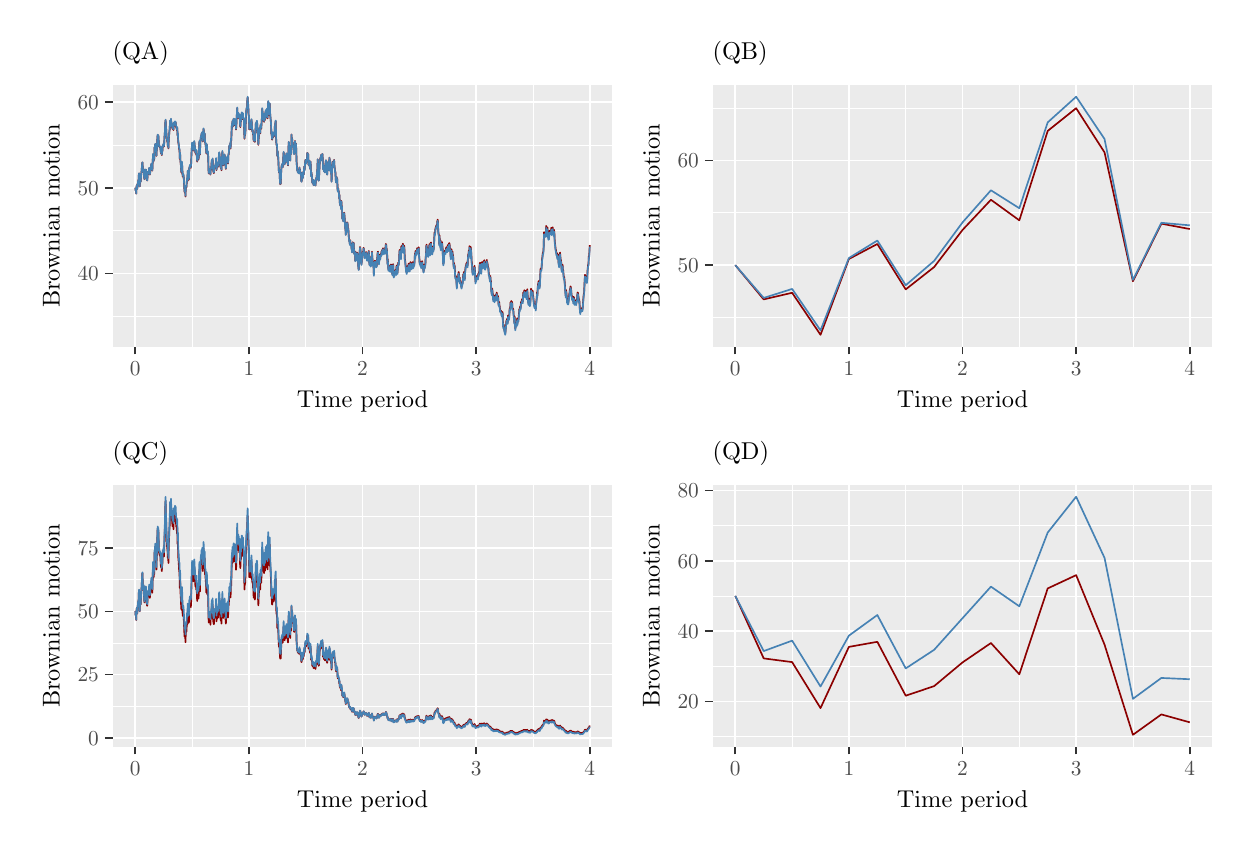
\begin{tikzpicture}[x=1pt,y=1pt]
\definecolor{fillColor}{RGB}{255,255,255}
\path[use as bounding box,fill=fillColor,fill opacity=0.00] (0,0) rectangle (433.62,289.08);
\begin{scope}
\path[clip] (  0.00,144.54) rectangle (216.81,289.08);
\definecolor{drawColor}{RGB}{255,255,255}
\definecolor{fillColor}{RGB}{255,255,255}

\path[draw=drawColor,line width= 0.6pt,line join=round,line cap=round,fill=fillColor] (  0.00,144.54) rectangle (216.81,289.08);
\end{scope}
\begin{scope}
\path[clip] ( 30.68,173.80) rectangle (211.31,268.42);
\definecolor{fillColor}{gray}{0.92}

\path[fill=fillColor] ( 30.68,173.80) rectangle (211.31,268.42);
\definecolor{drawColor}{RGB}{255,255,255}

\path[draw=drawColor,line width= 0.3pt,line join=round] ( 30.68,184.79) --
	(211.31,184.79);

\path[draw=drawColor,line width= 0.3pt,line join=round] ( 30.68,215.73) --
	(211.31,215.73);

\path[draw=drawColor,line width= 0.3pt,line join=round] ( 30.68,246.67) --
	(211.31,246.67);

\path[draw=drawColor,line width= 0.3pt,line join=round] ( 59.42,173.80) --
	( 59.42,268.42);

\path[draw=drawColor,line width= 0.3pt,line join=round] (100.47,173.80) --
	(100.47,268.42);

\path[draw=drawColor,line width= 0.3pt,line join=round] (141.52,173.80) --
	(141.52,268.42);

\path[draw=drawColor,line width= 0.3pt,line join=round] (182.57,173.80) --
	(182.57,268.42);

\path[draw=drawColor,line width= 0.6pt,line join=round] ( 30.68,200.26) --
	(211.31,200.26);

\path[draw=drawColor,line width= 0.6pt,line join=round] ( 30.68,231.20) --
	(211.31,231.20);

\path[draw=drawColor,line width= 0.6pt,line join=round] ( 30.68,262.13) --
	(211.31,262.13);

\path[draw=drawColor,line width= 0.6pt,line join=round] ( 38.89,173.80) --
	( 38.89,268.42);

\path[draw=drawColor,line width= 0.6pt,line join=round] ( 79.94,173.80) --
	( 79.94,268.42);

\path[draw=drawColor,line width= 0.6pt,line join=round] (121.00,173.80) --
	(121.00,268.42);

\path[draw=drawColor,line width= 0.6pt,line join=round] (162.05,173.80) --
	(162.05,268.42);

\path[draw=drawColor,line width= 0.6pt,line join=round] (203.10,173.80) --
	(203.10,268.42);
\definecolor{drawColor}{RGB}{139,0,0}

\path[draw=drawColor,line width= 0.6pt,line join=round] ( 38.89,231.20) --
	( 39.01,230.17) --
	( 39.12,230.46) --
	( 39.23,229.10) --
	( 39.35,231.68) --
	( 39.46,232.21) --
	( 39.58,230.86) --
	( 39.69,231.65) --
	( 39.80,232.85) --
	( 39.92,233.80) --
	( 40.03,233.28) --
	( 40.15,235.79) --
	( 40.26,236.44) --
	( 40.37,235.39) --
	( 40.49,231.71) --
	( 40.60,233.55) --
	( 40.72,233.47) --
	( 40.83,233.43) --
	( 40.94,234.99) --
	( 41.06,236.36) --
	( 41.17,237.36) --
	( 41.29,238.92) --
	( 41.40,240.25) --
	( 41.51,240.37) --
	( 41.63,236.96) --
	( 41.74,238.00) --
	( 41.86,237.90) --
	( 41.97,237.63) --
	( 42.08,235.14) --
	( 42.20,234.33) --
	( 42.31,235.02) --
	( 42.43,237.30) --
	( 42.54,237.11) --
	( 42.65,237.76) --
	( 42.77,237.66) --
	( 42.88,235.33) --
	( 43.00,234.63) --
	( 43.11,233.97) --
	( 43.22,233.86) --
	( 43.34,235.68) --
	( 43.45,236.96) --
	( 43.57,236.67) --
	( 43.68,236.24) --
	( 43.79,237.41) --
	( 43.91,238.34) --
	( 44.02,237.17) --
	( 44.14,235.96) --
	( 44.25,236.57) --
	( 44.36,237.86) --
	( 44.48,237.66) --
	( 44.59,239.16) --
	( 44.71,239.83) --
	( 44.82,238.77) --
	( 44.94,239.35) --
	( 45.05,237.41) --
	( 45.16,239.85) --
	( 45.28,243.29) --
	( 45.39,242.63) --
	( 45.51,240.81) --
	( 45.62,241.79) --
	( 45.73,241.54) --
	( 45.85,245.76) --
	( 45.96,245.68) --
	( 46.08,246.91) --
	( 46.19,246.95) --
	( 46.30,245.61) --
	( 46.42,245.94) --
	( 46.53,242.74) --
	( 46.65,245.31) --
	( 46.76,245.58) --
	( 46.87,249.48) --
	( 46.99,250.34) --
	( 47.10,249.04) --
	( 47.22,250.14) --
	( 47.33,248.43) --
	( 47.44,246.17) --
	( 47.56,246.68) --
	( 47.67,245.88) --
	( 47.79,245.87) --
	( 47.90,245.99) --
	( 48.01,244.93) --
	( 48.13,243.92) --
	( 48.24,243.67) --
	( 48.36,245.75) --
	( 48.47,243.04) --
	( 48.58,244.08) --
	( 48.70,244.66) --
	( 48.81,246.54) --
	( 48.93,245.99) --
	( 49.04,246.64) --
	( 49.15,247.11) --
	( 49.27,246.13) --
	( 49.38,248.30) --
	( 49.50,250.40) --
	( 49.61,251.68) --
	( 49.72,254.62) --
	( 49.84,255.66) --
	( 49.95,253.26) --
	( 50.07,252.19) --
	( 50.18,249.92) --
	( 50.29,249.05) --
	( 50.41,247.92) --
	( 50.52,247.98) --
	( 50.64,246.33) --
	( 50.75,246.61) --
	( 50.86,245.43) --
	( 50.98,248.60) --
	( 51.09,249.89) --
	( 51.21,251.55) --
	( 51.32,252.25) --
	( 51.44,255.39) --
	( 51.55,254.18) --
	( 51.66,253.31) --
	( 51.78,255.99) --
	( 51.89,254.75) --
	( 52.01,254.35) --
	( 52.12,253.61) --
	( 52.23,253.00) --
	( 52.35,252.47) --
	( 52.46,253.38) --
	( 52.58,253.04) --
	( 52.69,252.10) --
	( 52.80,254.59) --
	( 52.92,254.18) --
	( 53.03,253.83) --
	( 53.15,253.63) --
	( 53.26,254.96) --
	( 53.37,254.81) --
	( 53.49,254.73) --
	( 53.60,253.44) --
	( 53.72,252.83) --
	( 53.83,252.93) --
	( 53.94,251.83) --
	( 54.06,252.81) --
	( 54.17,250.00) --
	( 54.29,250.55) --
	( 54.40,247.74) --
	( 54.51,247.19) --
	( 54.63,246.24) --
	( 54.74,245.06) --
	( 54.86,244.95) --
	( 54.97,241.58) --
	( 55.08,243.63) --
	( 55.20,240.71) --
	( 55.31,239.90) --
	( 55.43,237.98) --
	( 55.54,236.70) --
	( 55.65,240.26) --
	( 55.77,240.28) --
	( 55.88,238.06) --
	( 56.00,235.28) --
	( 56.11,236.03) --
	( 56.22,235.99) --
	( 56.34,235.45) --
	( 56.45,233.89) --
	( 56.57,231.43) --
	( 56.68,229.68) --
	( 56.79,231.29) --
	( 56.91,230.27) --
	( 57.02,228.04) --
	( 57.14,231.05) --
	( 57.25,231.73) --
	( 57.36,231.33) --
	( 57.48,233.06) --
	( 57.59,234.52) --
	( 57.71,233.48) --
	( 57.82,237.17) --
	( 57.93,236.73) --
	( 58.05,234.33) --
	( 58.16,234.08) --
	( 58.28,234.42) --
	( 58.39,238.30) --
	( 58.51,238.47) --
	( 58.62,239.24) --
	( 58.73,239.10) --
	( 58.85,238.52) --
	( 58.96,238.45) --
	( 59.08,239.79) --
	( 59.19,243.40) --
	( 59.30,245.20) --
	( 59.42,247.36) --
	( 59.53,245.14) --
	( 59.65,246.89) --
	( 59.76,247.28) --
	( 59.87,244.65) --
	( 59.99,245.56) --
	( 60.10,245.27) --
	( 60.22,247.89) --
	( 60.33,246.50) --
	( 60.44,245.72) --
	( 60.56,244.07) --
	( 60.67,243.75) --
	( 60.79,244.45) --
	( 60.90,243.15) --
	( 61.01,244.60) --
	( 61.13,242.47) --
	( 61.24,240.64) --
	( 61.36,243.14) --
	( 61.47,241.36) --
	( 61.58,242.06) --
	( 61.70,241.39) --
	( 61.81,242.09) --
	( 61.93,245.06) --
	( 62.04,247.89) --
	( 62.15,247.29) --
	( 62.27,243.21) --
	( 62.38,247.65) --
	( 62.50,248.85) --
	( 62.61,249.82) --
	( 62.72,249.79) --
	( 62.84,250.71) --
	( 62.95,250.40) --
	( 63.07,251.17) --
	( 63.18,250.42) --
	( 63.29,247.92) --
	( 63.41,249.70) --
	( 63.52,252.49) --
	( 63.64,251.91) --
	( 63.75,249.60) --
	( 63.86,250.76) --
	( 63.98,250.67) --
	( 64.09,247.51) --
	( 64.21,247.50) --
	( 64.32,246.36) --
	( 64.43,245.74) --
	( 64.55,243.68) --
	( 64.66,246.88) --
	( 64.78,246.28) --
	( 64.89,243.42) --
	( 65.00,243.76) --
	( 65.12,244.21) --
	( 65.23,242.47) --
	( 65.35,237.48) --
	( 65.46,236.39) --
	( 65.58,237.35) --
	( 65.69,237.24) --
	( 65.80,237.06) --
	( 65.92,238.00) --
	( 66.03,235.99) --
	( 66.15,237.83) --
	( 66.26,237.82) --
	( 66.37,239.01) --
	( 66.49,240.79) --
	( 66.60,241.16) --
	( 66.72,239.64) --
	( 66.83,241.64) --
	( 66.94,238.19) --
	( 67.06,237.25) --
	( 67.17,236.81) --
	( 67.29,236.52) --
	( 67.40,238.24) --
	( 67.51,238.47) --
	( 67.63,239.15) --
	( 67.74,239.02) --
	( 67.86,238.59) --
	( 67.97,239.78) --
	( 68.08,241.75) --
	( 68.20,237.61) --
	( 68.31,238.58) --
	( 68.43,239.21) --
	( 68.54,238.47) --
	( 68.65,240.09) --
	( 68.77,239.41) --
	( 68.88,238.92) --
	( 69.00,240.38) --
	( 69.11,243.37) --
	( 69.22,243.84) --
	( 69.34,243.09) --
	( 69.45,241.00) --
	( 69.57,240.42) --
	( 69.68,238.80) --
	( 69.79,238.34) --
	( 69.91,239.01) --
	( 70.02,237.55) --
	( 70.14,242.10) --
	( 70.25,242.36) --
	( 70.36,244.34) --
	( 70.48,240.33) --
	( 70.59,241.61) --
	( 70.71,239.32) --
	( 70.82,240.90) --
	( 70.93,241.58) --
	( 71.05,240.86) --
	( 71.16,243.16) --
	( 71.28,241.93) --
	( 71.39,240.91) --
	( 71.50,239.18) --
	( 71.62,238.02) --
	( 71.73,239.63) --
	( 71.85,240.37) --
	( 71.96,242.11) --
	( 72.08,241.42) --
	( 72.19,242.07) --
	( 72.30,242.48) --
	( 72.42,240.00) --
	( 72.53,243.08) --
	( 72.65,243.31) --
	( 72.76,244.65) --
	( 72.87,246.34) --
	( 72.99,246.24) --
	( 73.10,245.69) --
	( 73.22,247.28) --
	( 73.33,245.39) --
	( 73.44,248.93) --
	( 73.56,248.23) --
	( 73.67,251.24) --
	( 73.79,254.03) --
	( 73.90,254.18) --
	( 74.01,255.23) --
	( 74.13,253.30) --
	( 74.24,253.90) --
	( 74.36,255.85) --
	( 74.47,256.03) --
	( 74.58,255.16) --
	( 74.70,253.92) --
	( 74.81,253.84) --
	( 74.93,255.84) --
	( 75.04,254.92) --
	( 75.15,254.68) --
	( 75.27,252.26) --
	( 75.38,253.17) --
	( 75.50,255.61) --
	( 75.61,258.45) --
	( 75.72,260.01) --
	( 75.84,256.42) --
	( 75.95,257.32) --
	( 76.07,258.18) --
	( 76.18,257.50) --
	( 76.29,257.81) --
	( 76.41,256.16) --
	( 76.52,257.44) --
	( 76.64,256.81) --
	( 76.75,253.84) --
	( 76.86,253.15) --
	( 76.98,255.69) --
	( 77.09,255.05) --
	( 77.21,256.43) --
	( 77.32,258.22) --
	( 77.43,258.22) --
	( 77.55,257.54) --
	( 77.66,256.52) --
	( 77.78,257.92) --
	( 77.89,255.89) --
	( 78.00,256.34) --
	( 78.12,255.78) --
	( 78.23,251.54) --
	( 78.35,248.96) --
	( 78.46,250.62) --
	( 78.57,250.26) --
	( 78.69,251.73) --
	( 78.80,255.24) --
	( 78.92,258.02) --
	( 79.03,259.32) --
	( 79.15,260.04) --
	( 79.26,259.66) --
	( 79.37,262.72) --
	( 79.49,263.88) --
	( 79.60,261.57) --
	( 79.72,261.25) --
	( 79.83,257.54) --
	( 79.94,257.16) --
	( 80.06,252.28) --
	( 80.17,254.72) --
	( 80.29,253.52) --
	( 80.40,252.71) --
	( 80.51,252.39) --
	( 80.63,253.52) --
	( 80.74,254.78) --
	( 80.86,255.84) --
	( 80.97,254.75) --
	( 81.08,252.20) --
	( 81.20,251.47) --
	( 81.31,251.97) --
	( 81.43,250.45) --
	( 81.54,250.31) --
	( 81.65,248.18) --
	( 81.77,248.15) --
	( 81.88,248.38) --
	( 82.00,248.10) --
	( 82.11,247.80) --
	( 82.22,251.00) --
	( 82.34,252.40) --
	( 82.45,254.46) --
	( 82.57,252.73) --
	( 82.68,253.02) --
	( 82.79,255.18) --
	( 82.91,255.06) --
	( 83.02,251.09) --
	( 83.14,251.71) --
	( 83.25,248.22) --
	( 83.36,246.75) --
	( 83.48,249.13) --
	( 83.59,250.25) --
	( 83.71,252.25) --
	( 83.82,252.81) --
	( 83.93,252.59) --
	( 84.05,250.88) --
	( 84.16,253.82) --
	( 84.28,253.89) --
	( 84.39,252.55) --
	( 84.50,254.15) --
	( 84.62,256.17) --
	( 84.73,259.78) --
	( 84.85,258.61) --
	( 84.96,257.85) --
	( 85.07,257.05) --
	( 85.19,256.33) --
	( 85.30,255.62) --
	( 85.42,255.05) --
	( 85.53,257.78) --
	( 85.65,256.44) --
	( 85.76,255.70) --
	( 85.87,256.92) --
	( 85.99,259.06) --
	( 86.10,257.57) --
	( 86.22,256.60) --
	( 86.33,257.58) --
	( 86.44,259.53) --
	( 86.56,259.03) --
	( 86.67,256.29) --
	( 86.79,259.55) --
	( 86.90,262.33) --
	( 87.01,260.93) --
	( 87.13,260.80) --
	( 87.24,257.40) --
	( 87.36,258.48) --
	( 87.47,261.59) --
	( 87.58,258.41) --
	( 87.70,256.91) --
	( 87.81,255.69) --
	( 87.93,254.40) --
	( 88.04,250.61) --
	( 88.15,251.53) --
	( 88.27,248.71) --
	( 88.38,248.66) --
	( 88.50,249.73) --
	( 88.61,249.36) --
	( 88.72,250.98) --
	( 88.84,250.92) --
	( 88.95,249.73) --
	( 89.07,250.90) --
	( 89.18,250.10) --
	( 89.29,253.36) --
	( 89.41,253.32) --
	( 89.52,254.90) --
	( 89.64,255.28) --
	( 89.75,249.69) --
	( 89.86,247.21) --
	( 89.98,246.43) --
	( 90.09,246.85) --
	( 90.21,242.69) --
	( 90.32,244.37) --
	( 90.43,243.29) --
	( 90.55,241.97) --
	( 90.66,239.27) --
	( 90.78,236.78) --
	( 90.89,236.87) --
	( 91.00,237.72) --
	( 91.12,234.19) --
	( 91.23,232.52) --
	( 91.35,233.39) --
	( 91.46,232.64) --
	( 91.57,236.23) --
	( 91.69,238.34) --
	( 91.80,239.35) --
	( 91.92,239.35) --
	( 92.03,239.82) --
	( 92.14,238.60) --
	( 92.26,239.66) --
	( 92.37,242.22) --
	( 92.49,244.11) --
	( 92.60,242.68) --
	( 92.72,239.85) --
	( 92.83,239.66) --
	( 92.94,240.41) --
	( 93.06,242.75) --
	( 93.17,240.45) --
	( 93.29,241.07) --
	( 93.40,241.46) --
	( 93.51,243.54) --
	( 93.63,243.48) --
	( 93.74,242.85) --
	( 93.86,240.84) --
	( 93.97,239.94) --
	( 94.08,239.31) --
	( 94.20,243.38) --
	( 94.31,247.73) --
	( 94.43,247.42) --
	( 94.54,245.54) --
	( 94.65,242.05) --
	( 94.77,242.94) --
	( 94.88,241.03) --
	( 95.00,245.03) --
	( 95.11,243.46) --
	( 95.22,243.64) --
	( 95.34,250.48) --
	( 95.45,248.45) --
	( 95.57,249.00) --
	( 95.68,246.99) --
	( 95.79,247.61) --
	( 95.91,246.03) --
	( 96.02,246.16) --
	( 96.14,245.62) --
	( 96.25,243.51) --
	( 96.36,243.53) --
	( 96.48,245.27) --
	( 96.59,248.12) --
	( 96.71,245.65) --
	( 96.82,245.19) --
	( 96.93,247.26) --
	( 97.05,245.25) --
	( 97.16,240.81) --
	( 97.28,239.18) --
	( 97.39,237.53) --
	( 97.50,237.60) --
	( 97.62,236.90) --
	( 97.73,237.29) --
	( 97.85,236.56) --
	( 97.96,237.19) --
	( 98.07,236.56) --
	( 98.19,238.57) --
	( 98.30,237.31) --
	( 98.42,237.79) --
	( 98.53,236.29) --
	( 98.64,236.63) --
	( 98.76,236.54) --
	( 98.87,233.71) --
	( 98.99,233.47) --
	( 99.10,235.42) --
	( 99.22,236.56) --
	( 99.33,236.79) --
	( 99.44,234.78) --
	( 99.56,236.73) --
	( 99.67,236.86) --
	( 99.79,236.09) --
	( 99.90,238.87) --
	(100.01,237.55) --
	(100.13,238.05) --
	(100.24,240.24) --
	(100.36,241.27) --
	(100.47,240.73) --
	(100.58,240.00) --
	(100.70,240.60) --
	(100.81,241.49) --
	(100.93,241.51) --
	(101.04,243.81) --
	(101.15,243.68) --
	(101.27,242.44) --
	(101.38,243.38) --
	(101.50,239.54) --
	(101.61,240.21) --
	(101.72,241.06) --
	(101.84,240.66) --
	(101.95,238.73) --
	(102.07,238.05) --
	(102.18,240.70) --
	(102.29,239.41) --
	(102.41,235.44) --
	(102.52,236.80) --
	(102.64,235.95) --
	(102.75,235.08) --
	(102.86,233.05) --
	(102.98,233.01) --
	(103.09,234.16) --
	(103.21,233.18) --
	(103.32,232.17) --
	(103.43,233.97) --
	(103.55,233.55) --
	(103.66,233.28) --
	(103.78,232.24) --
	(103.89,233.72) --
	(104.00,232.07) --
	(104.12,233.46) --
	(104.23,234.79) --
	(104.35,234.00) --
	(104.46,235.41) --
	(104.57,237.06) --
	(104.69,238.03) --
	(104.80,241.50) --
	(104.92,238.12) --
	(105.03,236.14) --
	(105.14,233.83) --
	(105.26,234.10) --
	(105.37,236.74) --
	(105.49,239.59) --
	(105.60,240.43) --
	(105.71,241.94) --
	(105.83,241.68) --
	(105.94,242.49) --
	(106.06,243.14) --
	(106.17,241.80) --
	(106.29,241.28) --
	(106.40,241.04) --
	(106.51,243.46) --
	(106.63,241.64) --
	(106.74,237.99) --
	(106.86,239.29) --
	(106.97,237.89) --
	(107.08,237.14) --
	(107.20,238.67) --
	(107.31,237.36) --
	(107.43,236.78) --
	(107.54,239.33) --
	(107.65,240.23) --
	(107.77,241.16) --
	(107.88,240.91) --
	(108.00,238.94) --
	(108.11,236.39) --
	(108.22,236.01) --
	(108.34,239.40) --
	(108.45,239.77) --
	(108.57,240.04) --
	(108.68,240.61) --
	(108.79,239.94) --
	(108.91,237.53) --
	(109.02,242.13) --
	(109.14,241.38) --
	(109.25,240.86) --
	(109.36,237.77) --
	(109.48,237.34) --
	(109.59,236.92) --
	(109.71,236.47) --
	(109.82,233.48) --
	(109.93,236.45) --
	(110.05,239.45) --
	(110.16,240.62) --
	(110.28,238.72) --
	(110.39,239.94) --
	(110.50,239.51) --
	(110.62,238.95) --
	(110.73,241.29) --
	(110.85,239.16) --
	(110.96,238.28) --
	(111.07,237.03) --
	(111.19,237.05) --
	(111.30,234.40) --
	(111.42,233.23) --
	(111.53,234.41) --
	(111.64,235.17) --
	(111.76,233.55) --
	(111.87,234.47) --
	(111.99,230.46) --
	(112.10,229.90) --
	(112.21,231.05) --
	(112.33,229.97) --
	(112.44,229.90) --
	(112.56,227.34) --
	(112.67,228.68) --
	(112.79,225.74) --
	(112.90,225.22) --
	(113.01,224.81) --
	(113.13,224.90) --
	(113.24,223.61) --
	(113.36,226.46) --
	(113.47,224.21) --
	(113.58,224.60) --
	(113.70,220.07) --
	(113.81,220.07) --
	(113.93,220.84) --
	(114.04,219.19) --
	(114.15,220.24) --
	(114.27,220.74) --
	(114.38,222.22) --
	(114.50,220.92) --
	(114.61,219.45) --
	(114.72,216.79) --
	(114.84,216.31) --
	(114.95,214.34) --
	(115.07,215.34) --
	(115.18,215.44) --
	(115.29,218.67) --
	(115.41,216.94) --
	(115.52,218.69) --
	(115.64,217.90) --
	(115.75,215.73) --
	(115.86,216.57) --
	(115.98,214.46) --
	(116.09,212.93) --
	(116.21,211.87) --
	(116.32,212.16) --
	(116.43,210.74) --
	(116.55,212.26) --
	(116.66,210.55) --
	(116.78,210.85) --
	(116.89,211.04) --
	(117.00,209.53) --
	(117.12,208.93) --
	(117.23,208.01) --
	(117.35,209.34) --
	(117.46,211.52) --
	(117.57,210.04) --
	(117.69,211.35) --
	(117.80,211.24) --
	(117.92,208.47) --
	(118.03,207.41) --
	(118.14,208.04) --
	(118.26,208.24) --
	(118.37,204.88) --
	(118.49,205.66) --
	(118.60,206.55) --
	(118.71,206.13) --
	(118.83,205.16) --
	(118.94,207.85) --
	(119.06,207.72) --
	(119.17,207.69) --
	(119.28,206.14) --
	(119.40,204.31) --
	(119.51,202.27) --
	(119.63,201.70) --
	(119.74,203.50) --
	(119.86,205.87) --
	(119.97,208.01) --
	(120.08,209.82) --
	(120.20,209.48) --
	(120.31,207.76) --
	(120.43,207.30) --
	(120.54,204.01) --
	(120.65,203.58) --
	(120.77,205.82) --
	(120.88,205.99) --
	(121.00,207.49) --
	(121.11,208.16) --
	(121.22,207.07) --
	(121.34,209.49) --
	(121.45,209.37) --
	(121.57,208.01) --
	(121.68,208.10) --
	(121.79,206.00) --
	(121.91,207.18) --
	(122.02,207.86) --
	(122.14,207.36) --
	(122.25,206.69) --
	(122.36,207.97) --
	(122.48,206.50) --
	(122.59,205.15) --
	(122.71,205.72) --
	(122.82,205.10) --
	(122.93,206.35) --
	(123.05,206.07) --
	(123.16,207.71) --
	(123.28,208.39) --
	(123.39,205.30) --
	(123.50,203.49) --
	(123.62,205.21) --
	(123.73,206.14) --
	(123.85,204.82) --
	(123.96,203.01) --
	(124.07,204.39) --
	(124.19,203.29) --
	(124.30,205.71) --
	(124.42,208.14) --
	(124.53,206.13) --
	(124.64,204.97) --
	(124.76,203.28) --
	(124.87,204.17) --
	(124.99,202.44) --
	(125.10,199.76) --
	(125.21,202.41) --
	(125.33,203.74) --
	(125.44,204.84) --
	(125.56,203.93) --
	(125.67,203.91) --
	(125.78,204.74) --
	(125.90,203.01) --
	(126.01,202.84) --
	(126.13,203.07) --
	(126.24,205.34) --
	(126.36,206.21) --
	(126.47,207.96) --
	(126.58,208.15) --
	(126.70,206.61) --
	(126.81,206.14) --
	(126.93,203.88) --
	(127.04,205.12) --
	(127.15,207.05) --
	(127.27,206.96) --
	(127.38,205.61) --
	(127.50,207.09) --
	(127.61,207.27) --
	(127.72,206.73) --
	(127.84,208.28) --
	(127.95,207.22) --
	(128.07,208.80) --
	(128.18,207.63) --
	(128.29,208.16) --
	(128.41,209.40) --
	(128.52,207.53) --
	(128.64,208.08) --
	(128.75,207.91) --
	(128.86,208.85) --
	(128.98,207.74) --
	(129.09,207.62) --
	(129.21,209.53) --
	(129.32,209.76) --
	(129.43,210.92) --
	(129.55,210.60) --
	(129.66,209.14) --
	(129.78,209.12) --
	(129.89,207.41) --
	(130.00,203.87) --
	(130.12,205.44) --
	(130.23,203.97) --
	(130.35,201.53) --
	(130.46,202.84) --
	(130.57,202.82) --
	(130.69,202.02) --
	(130.80,201.77) --
	(130.92,201.21) --
	(131.03,202.52) --
	(131.14,203.48) --
	(131.26,201.18) --
	(131.37,201.64) --
	(131.49,202.59) --
	(131.60,203.48) --
	(131.71,200.27) --
	(131.83,199.96) --
	(131.94,202.55) --
	(132.06,203.61) --
	(132.17,201.33) --
	(132.28,199.15) --
	(132.40,199.78) --
	(132.51,199.55) --
	(132.63,200.80) --
	(132.74,201.18) --
	(132.85,201.28) --
	(132.97,201.51) --
	(133.08,201.72) --
	(133.20,200.05) --
	(133.31,203.14) --
	(133.43,201.26) --
	(133.54,201.24) --
	(133.65,200.51) --
	(133.77,202.88) --
	(133.88,204.23) --
	(134.00,203.47) --
	(134.11,203.73) --
	(134.22,205.30) --
	(134.34,208.36) --
	(134.45,208.78) --
	(134.57,207.33) --
	(134.68,205.97) --
	(134.79,208.73) --
	(134.91,205.87) --
	(135.02,210.09) --
	(135.14,209.72) --
	(135.25,209.07) --
	(135.36,209.29) --
	(135.48,210.59) --
	(135.59,211.01) --
	(135.71,208.26) --
	(135.82,208.75) --
	(135.93,209.37) --
	(136.05,210.29) --
	(136.16,208.83) --
	(136.28,205.56) --
	(136.39,205.11) --
	(136.50,203.83) --
	(136.62,202.80) --
	(136.73,201.53) --
	(136.85,201.00) --
	(136.96,200.59) --
	(137.07,201.62) --
	(137.19,202.93) --
	(137.30,201.86) --
	(137.42,201.45) --
	(137.53,201.92) --
	(137.64,203.78) --
	(137.76,203.69) --
	(137.87,201.43) --
	(137.99,201.73) --
	(138.10,201.56) --
	(138.21,203.91) --
	(138.33,204.37) --
	(138.44,203.53) --
	(138.56,202.93) --
	(138.67,202.25) --
	(138.78,202.49) --
	(138.90,202.72) --
	(139.01,203.94) --
	(139.13,204.36) --
	(139.24,203.86) --
	(139.35,202.60) --
	(139.47,203.44) --
	(139.58,203.35) --
	(139.70,203.58) --
	(139.81,205.06) --
	(139.93,207.45) --
	(140.04,206.14) --
	(140.15,208.39) --
	(140.27,207.19) --
	(140.38,207.55) --
	(140.50,207.85) --
	(140.61,207.46) --
	(140.72,209.39) --
	(140.84,208.46) --
	(140.95,209.38) --
	(141.07,209.35) --
	(141.18,208.04) --
	(141.29,209.73) --
	(141.41,206.82) --
	(141.52,206.10) --
	(141.64,204.00) --
	(141.75,204.26) --
	(141.86,204.61) --
	(141.98,203.10) --
	(142.09,203.96) --
	(142.21,202.57) --
	(142.32,203.45) --
	(142.43,203.76) --
	(142.55,204.71) --
	(142.66,203.44) --
	(142.78,203.56) --
	(142.89,202.94) --
	(143.00,200.99) --
	(143.12,201.18) --
	(143.23,203.53) --
	(143.35,202.66) --
	(143.46,202.39) --
	(143.57,203.30) --
	(143.69,203.34) --
	(143.80,205.96) --
	(143.92,206.96) --
	(144.03,210.18) --
	(144.14,210.67) --
	(144.26,209.07) --
	(144.37,209.65) --
	(144.49,208.35) --
	(144.60,206.95) --
	(144.71,206.68) --
	(144.83,207.96) --
	(144.94,208.43) --
	(145.06,209.56) --
	(145.17,210.84) --
	(145.28,210.59) --
	(145.40,207.23) --
	(145.51,208.33) --
	(145.63,211.37) --
	(145.74,211.45) --
	(145.85,209.52) --
	(145.97,209.00) --
	(146.08,207.70) --
	(146.20,207.63) --
	(146.31,208.56) --
	(146.42,209.77) --
	(146.54,210.09) --
	(146.65,208.77) --
	(146.77,209.91) --
	(146.88,211.81) --
	(147.00,215.05) --
	(147.11,214.32) --
	(147.22,215.01) --
	(147.34,216.75) --
	(147.45,216.57) --
	(147.57,217.34) --
	(147.68,217.65) --
	(147.79,217.44) --
	(147.91,217.69) --
	(148.02,219.12) --
	(148.14,219.73) --
	(148.25,219.02) --
	(148.36,215.69) --
	(148.48,214.52) --
	(148.59,214.48) --
	(148.71,210.86) --
	(148.82,214.02) --
	(148.93,211.88) --
	(149.05,210.22) --
	(149.16,212.28) --
	(149.28,209.18) --
	(149.39,210.21) --
	(149.50,209.72) --
	(149.62,210.35) --
	(149.73,211.59) --
	(149.85,210.22) --
	(149.96,209.23) --
	(150.07,205.09) --
	(150.19,203.79) --
	(150.30,204.29) --
	(150.42,204.97) --
	(150.53,207.73) --
	(150.64,207.82) --
	(150.76,208.45) --
	(150.87,208.55) --
	(150.99,207.87) --
	(151.10,208.90) --
	(151.21,209.54) --
	(151.33,209.72) --
	(151.44,208.57) --
	(151.56,208.51) --
	(151.67,209.59) --
	(151.78,210.53) --
	(151.90,209.85) --
	(152.01,208.90) --
	(152.13,209.61) --
	(152.24,211.08) --
	(152.35,211.25) --
	(152.47,210.80) --
	(152.58,209.55) --
	(152.70,208.96) --
	(152.81,206.89) --
	(152.92,205.93) --
	(153.04,207.48) --
	(153.15,209.02) --
	(153.27,207.80) --
	(153.38,208.09) --
	(153.50,208.18) --
	(153.61,205.88) --
	(153.72,206.98) --
	(153.84,204.37) --
	(153.95,202.70) --
	(154.07,204.02) --
	(154.18,203.29) --
	(154.29,203.00) --
	(154.41,200.85) --
	(154.52,198.95) --
	(154.64,199.40) --
	(154.75,199.17) --
	(154.86,198.40) --
	(154.98,196.69) --
	(155.09,195.30) --
	(155.21,197.87) --
	(155.32,197.45) --
	(155.43,198.43) --
	(155.55,199.44) --
	(155.66,200.42) --
	(155.78,200.80) --
	(155.89,199.16) --
	(156.00,197.86) --
	(156.12,198.82) --
	(156.23,197.14) --
	(156.35,197.80) --
	(156.46,197.11) --
	(156.57,196.60) --
	(156.69,195.60) --
	(156.80,195.31) --
	(156.92,196.40) --
	(157.03,196.97) --
	(157.14,196.67) --
	(157.26,197.77) --
	(157.37,199.90) --
	(157.49,199.88) --
	(157.60,200.49) --
	(157.71,200.85) --
	(157.83,199.56) --
	(157.94,198.36) --
	(158.06,200.85) --
	(158.17,202.00) --
	(158.28,202.98) --
	(158.40,203.17) --
	(158.51,203.81) --
	(158.63,204.01) --
	(158.74,204.06) --
	(158.85,204.35) --
	(158.97,202.99) --
	(159.08,206.22) --
	(159.20,207.32) --
	(159.31,206.96) --
	(159.42,208.63) --
	(159.54,207.76) --
	(159.65,210.14) --
	(159.77,209.58) --
	(159.88,206.35) --
	(159.99,208.23) --
	(160.11,209.80) --
	(160.22,208.71) --
	(160.34,206.75) --
	(160.45,204.25) --
	(160.57,203.88) --
	(160.68,201.44) --
	(160.79,200.36) --
	(160.91,200.57) --
	(161.02,201.68) --
	(161.14,200.60) --
	(161.25,200.43) --
	(161.36,200.76) --
	(161.48,203.02) --
	(161.59,201.74) --
	(161.71,199.64) --
	(161.82,197.26) --
	(161.93,197.96) --
	(162.05,197.88) --
	(162.16,198.86) --
	(162.28,198.67) --
	(162.39,199.17) --
	(162.50,199.46) --
	(162.62,199.48) --
	(162.73,198.67) --
	(162.85,200.30) --
	(162.96,199.76) --
	(163.07,200.63) --
	(163.19,200.83) --
	(163.30,203.18) --
	(163.42,204.13) --
	(163.53,203.67) --
	(163.64,203.65) --
	(163.76,203.48) --
	(163.87,200.70) --
	(163.99,202.94) --
	(164.10,204.35) --
	(164.21,203.32) --
	(164.33,203.82) --
	(164.44,204.14) --
	(164.56,202.62) --
	(164.67,204.61) --
	(164.78,204.27) --
	(164.90,204.51) --
	(165.01,205.05) --
	(165.13,203.70) --
	(165.24,202.25) --
	(165.35,202.18) --
	(165.47,202.93) --
	(165.58,203.02) --
	(165.70,203.96) --
	(165.81,204.41) --
	(165.92,205.14) --
	(166.04,203.24) --
	(166.15,204.14) --
	(166.27,203.08) --
	(166.38,202.45) --
	(166.49,202.30) --
	(166.61,200.13) --
	(166.72,199.99) --
	(166.84,199.42) --
	(166.95,198.48) --
	(167.06,197.76) --
	(167.18,199.36) --
	(167.29,197.73) --
	(167.41,197.45) --
	(167.52,194.34) --
	(167.64,193.49) --
	(167.75,192.87) --
	(167.86,194.77) --
	(167.98,193.57) --
	(168.09,192.50) --
	(168.21,190.79) --
	(168.32,191.00) --
	(168.43,192.40) --
	(168.55,190.94) --
	(168.66,190.42) --
	(168.78,192.06) --
	(168.89,191.23) --
	(169.00,192.05) --
	(169.12,192.52) --
	(169.23,190.93) --
	(169.35,192.40) --
	(169.46,193.37) --
	(169.57,192.76) --
	(169.69,191.65) --
	(169.80,191.18) --
	(169.92,192.16) --
	(170.03,191.46) --
	(170.14,189.21) --
	(170.26,189.03) --
	(170.37,189.95) --
	(170.49,188.56) --
	(170.60,188.28) --
	(170.71,186.84) --
	(170.83,186.97) --
	(170.94,186.81) --
	(171.06,186.76) --
	(171.17,186.04) --
	(171.28,185.21) --
	(171.40,186.21) --
	(171.51,186.33) --
	(171.63,186.11) --
	(171.74,182.45) --
	(171.85,181.03) --
	(171.97,181.87) --
	(172.08,181.41) --
	(172.20,180.08) --
	(172.31,179.59) --
	(172.42,179.18) --
	(172.54,178.63) --
	(172.65,179.16) --
	(172.77,180.82) --
	(172.88,181.90) --
	(172.99,183.29) --
	(173.11,182.91) --
	(173.22,183.86) --
	(173.34,182.75) --
	(173.45,182.59) --
	(173.56,185.05) --
	(173.68,185.03) --
	(173.79,184.68) --
	(173.91,184.01) --
	(174.02,184.88) --
	(174.14,187.31) --
	(174.25,187.78) --
	(174.36,187.47) --
	(174.48,189.91) --
	(174.59,188.98) --
	(174.71,190.32) --
	(174.82,189.81) --
	(174.93,188.59) --
	(175.05,190.04) --
	(175.16,187.90) --
	(175.28,187.53) --
	(175.39,187.54) --
	(175.50,187.02) --
	(175.62,185.12) --
	(175.73,184.38) --
	(175.85,182.62) --
	(175.96,184.79) --
	(176.07,182.68) --
	(176.19,180.35) --
	(176.30,181.11) --
	(176.42,182.11) --
	(176.53,181.88) --
	(176.64,181.65) --
	(176.76,182.45) --
	(176.87,184.02) --
	(176.99,182.22) --
	(177.10,183.68) --
	(177.21,183.90) --
	(177.33,183.51) --
	(177.44,184.94) --
	(177.56,186.01) --
	(177.67,187.49) --
	(177.78,187.14) --
	(177.90,188.05) --
	(178.01,188.39) --
	(178.13,187.77) --
	(178.24,189.85) --
	(178.35,190.03) --
	(178.47,189.96) --
	(178.58,190.59) --
	(178.70,191.05) --
	(178.81,190.20) --
	(178.92,190.13) --
	(179.04,193.29) --
	(179.15,193.19) --
	(179.27,192.82) --
	(179.38,193.72) --
	(179.49,194.21) --
	(179.61,193.54) --
	(179.72,192.20) --
	(179.84,193.23) --
	(179.95,193.37) --
	(180.06,193.96) --
	(180.18,193.60) --
	(180.29,191.57) --
	(180.41,191.65) --
	(180.52,194.58) --
	(180.63,192.77) --
	(180.75,191.56) --
	(180.86,189.94) --
	(180.98,189.50) --
	(181.09,191.15) --
	(181.21,190.96) --
	(181.32,190.65) --
	(181.43,189.10) --
	(181.55,189.17) --
	(181.66,190.40) --
	(181.78,193.14) --
	(181.89,194.76) --
	(182.00,193.68) --
	(182.12,193.05) --
	(182.23,193.79) --
	(182.35,193.77) --
	(182.46,194.11) --
	(182.57,192.49) --
	(182.69,191.96) --
	(182.80,190.83) --
	(182.92,189.71) --
	(183.03,188.85) --
	(183.14,188.35) --
	(183.26,188.34) --
	(183.37,189.08) --
	(183.49,188.47) --
	(183.60,187.46) --
	(183.71,189.36) --
	(183.83,190.54) --
	(183.94,191.38) --
	(184.06,193.45) --
	(184.17,192.24) --
	(184.28,194.76) --
	(184.40,196.29) --
	(184.51,196.68) --
	(184.63,197.46) --
	(184.74,197.53) --
	(184.85,197.39) --
	(184.97,195.39) --
	(185.08,196.32) --
	(185.20,199.05) --
	(185.31,201.77) --
	(185.42,201.98) --
	(185.54,201.84) --
	(185.65,202.07) --
	(185.77,203.59) --
	(185.88,205.57) --
	(185.99,206.12) --
	(186.11,207.65) --
	(186.22,207.60) --
	(186.34,208.28) --
	(186.45,209.93) --
	(186.56,215.14) --
	(186.68,215.06) --
	(186.79,214.08) --
	(186.91,214.72) --
	(187.02,214.12) --
	(187.13,215.04) --
	(187.25,215.53) --
	(187.36,217.46) --
	(187.48,216.04) --
	(187.59,214.27) --
	(187.71,216.55) --
	(187.82,216.88) --
	(187.93,215.51) --
	(188.05,213.94) --
	(188.16,213.14) --
	(188.28,213.98) --
	(188.39,213.21) --
	(188.50,215.15) --
	(188.62,215.50) --
	(188.73,215.78) --
	(188.85,215.75) --
	(188.96,215.31) --
	(189.07,215.05) --
	(189.19,216.75) --
	(189.30,214.77) --
	(189.42,216.36) --
	(189.53,215.83) --
	(189.64,216.91) --
	(189.76,216.81) --
	(189.87,214.83) --
	(189.99,215.33) --
	(190.10,214.39) --
	(190.21,216.03) --
	(190.33,214.81) --
	(190.44,212.22) --
	(190.56,211.00) --
	(190.67,210.18) --
	(190.78,209.01) --
	(190.90,208.67) --
	(191.01,207.84) --
	(191.13,207.27) --
	(191.24,207.71) --
	(191.35,206.10) --
	(191.47,207.14) --
	(191.58,207.13) --
	(191.70,207.07) --
	(191.81,204.29) --
	(191.92,203.88) --
	(192.04,203.13) --
	(192.15,204.26) --
	(192.27,206.14) --
	(192.38,207.82) --
	(192.49,206.28) --
	(192.61,205.19) --
	(192.72,205.06) --
	(192.84,203.63) --
	(192.95,201.49) --
	(193.06,202.53) --
	(193.18,202.61) --
	(193.29,203.42) --
	(193.41,201.82) --
	(193.52,201.36) --
	(193.63,199.82) --
	(193.75,198.74) --
	(193.86,199.03) --
	(193.98,197.98) --
	(194.09,196.71) --
	(194.20,195.06) --
	(194.32,193.27) --
	(194.43,192.21) --
	(194.55,194.30) --
	(194.66,193.48) --
	(194.78,192.11) --
	(194.89,190.40) --
	(195.00,190.22) --
	(195.12,189.74) --
	(195.23,190.03) --
	(195.35,189.69) --
	(195.46,190.72) --
	(195.57,191.59) --
	(195.69,192.87) --
	(195.80,193.16) --
	(195.92,194.53) --
	(196.03,194.43) --
	(196.14,195.59) --
	(196.26,195.38) --
	(196.37,194.53) --
	(196.49,193.01) --
	(196.60,192.14) --
	(196.71,191.22) --
	(196.83,191.92) --
	(196.94,191.85) --
	(197.06,191.08) --
	(197.17,189.99) --
	(197.28,191.81) --
	(197.40,191.51) --
	(197.51,190.00) --
	(197.63,189.48) --
	(197.74,189.59) --
	(197.85,190.58) --
	(197.97,190.47) --
	(198.08,190.60) --
	(198.20,189.35) --
	(198.31,190.29) --
	(198.42,190.41) --
	(198.54,191.29) --
	(198.65,193.17) --
	(198.77,193.38) --
	(198.88,193.03) --
	(198.99,192.08) --
	(199.11,191.38) --
	(199.22,190.27) --
	(199.34,190.71) --
	(199.45,188.95) --
	(199.56,186.89) --
	(199.68,186.11) --
	(199.79,187.37) --
	(199.91,187.50) --
	(200.02,186.92) --
	(200.13,187.70) --
	(200.25,187.28) --
	(200.36,187.14) --
	(200.48,187.22) --
	(200.59,188.49) --
	(200.70,190.02) --
	(200.82,191.56) --
	(200.93,192.75) --
	(201.05,193.14) --
	(201.16,195.47) --
	(201.28,198.05) --
	(201.39,199.76) --
	(201.50,199.47) --
	(201.62,198.12) --
	(201.73,198.36) --
	(201.85,197.64) --
	(201.96,197.99) --
	(202.07,197.28) --
	(202.19,198.45) --
	(202.30,201.29) --
	(202.42,202.56) --
	(202.53,203.54) --
	(202.64,203.58) --
	(202.76,206.53) --
	(202.87,206.41) --
	(202.99,208.31) --
	(203.10,210.50);
\definecolor{drawColor}{RGB}{70,130,180}

\path[draw=drawColor,line width= 0.6pt,line join=round] ( 38.89,231.20) --
	( 39.01,230.18) --
	( 39.12,230.47) --
	( 39.23,229.12) --
	( 39.35,231.68) --
	( 39.46,232.22) --
	( 39.58,230.88) --
	( 39.69,231.67) --
	( 39.80,232.88) --
	( 39.92,233.83) --
	( 40.03,233.32) --
	( 40.15,235.82) --
	( 40.26,236.47) --
	( 40.37,235.42) --
	( 40.49,231.72) --
	( 40.60,233.56) --
	( 40.72,233.48) --
	( 40.83,233.45) --
	( 40.94,235.02) --
	( 41.06,236.39) --
	( 41.17,237.39) --
	( 41.29,238.95) --
	( 41.40,240.29) --
	( 41.51,240.41) --
	( 41.63,236.98) --
	( 41.74,238.03) --
	( 41.86,237.93) --
	( 41.97,237.67) --
	( 42.08,235.17) --
	( 42.20,234.37) --
	( 42.31,235.06) --
	( 42.43,237.33) --
	( 42.54,237.16) --
	( 42.65,237.82) --
	( 42.77,237.72) --
	( 42.88,235.39) --
	( 43.00,234.69) --
	( 43.11,234.03) --
	( 43.22,233.94) --
	( 43.34,235.76) --
	( 43.45,237.04) --
	( 43.57,236.76) --
	( 43.68,236.33) --
	( 43.79,237.51) --
	( 43.91,238.45) --
	( 44.02,237.28) --
	( 44.14,236.08) --
	( 44.25,236.69) --
	( 44.36,237.99) --
	( 44.48,237.80) --
	( 44.59,239.29) --
	( 44.71,239.98) --
	( 44.82,238.92) --
	( 44.94,239.51) --
	( 45.05,237.57) --
	( 45.16,240.00) --
	( 45.28,243.41) --
	( 45.39,242.76) --
	( 45.51,240.93) --
	( 45.62,241.92) --
	( 45.73,241.69) --
	( 45.85,245.86) --
	( 45.96,245.79) --
	( 46.08,247.02) --
	( 46.19,247.07) --
	( 46.30,245.74) --
	( 46.42,246.07) --
	( 46.53,242.85) --
	( 46.65,245.42) --
	( 46.76,245.69) --
	( 46.87,249.56) --
	( 46.99,250.43) --
	( 47.10,249.13) --
	( 47.22,250.24) --
	( 47.33,248.53) --
	( 47.44,246.26) --
	( 47.56,246.78) --
	( 47.67,245.98) --
	( 47.79,245.99) --
	( 47.90,246.12) --
	( 48.01,245.07) --
	( 48.13,244.06) --
	( 48.24,243.82) --
	( 48.36,245.89) --
	( 48.47,243.18) --
	( 48.58,244.22) --
	( 48.70,244.81) --
	( 48.81,246.69) --
	( 48.93,246.15) --
	( 49.04,246.81) --
	( 49.15,247.29) --
	( 49.27,246.31) --
	( 49.38,248.47) --
	( 49.50,250.57) --
	( 49.61,251.85) --
	( 49.72,254.78) --
	( 49.84,255.83) --
	( 49.95,253.42) --
	( 50.07,252.35) --
	( 50.18,250.09) --
	( 50.29,249.22) --
	( 50.41,248.09) --
	( 50.52,248.17) --
	( 50.64,246.52) --
	( 50.75,246.81) --
	( 50.86,245.63) --
	( 50.98,248.78) --
	( 51.09,250.08) --
	( 51.21,251.74) --
	( 51.32,252.45) --
	( 51.44,255.57) --
	( 51.55,254.37) --
	( 51.66,253.50) --
	( 51.78,256.17) --
	( 51.89,254.94) --
	( 52.01,254.55) --
	( 52.12,253.82) --
	( 52.23,253.22) --
	( 52.35,252.70) --
	( 52.46,253.62) --
	( 52.58,253.28) --
	( 52.69,252.34) --
	( 52.80,254.83) --
	( 52.92,254.43) --
	( 53.03,254.09) --
	( 53.15,253.90) --
	( 53.26,255.23) --
	( 53.37,255.09) --
	( 53.49,255.02) --
	( 53.60,253.74) --
	( 53.72,253.14) --
	( 53.83,253.25) --
	( 53.94,252.16) --
	( 54.06,253.14) --
	( 54.17,250.32) --
	( 54.29,250.88) --
	( 54.40,248.06) --
	( 54.51,247.52) --
	( 54.63,246.56) --
	( 54.74,245.40) --
	( 54.86,245.30) --
	( 54.97,241.90) --
	( 55.08,243.95) --
	( 55.20,241.01) --
	( 55.31,240.21) --
	( 55.43,238.29) --
	( 55.54,237.01) --
	( 55.65,240.53) --
	( 55.77,240.56) --
	( 55.88,238.34) --
	( 56.00,235.55) --
	( 56.11,236.30) --
	( 56.22,236.27) --
	( 56.34,235.74) --
	( 56.45,234.18) --
	( 56.57,231.71) --
	( 56.68,229.96) --
	( 56.79,231.57) --
	( 56.91,230.56) --
	( 57.02,228.31) --
	( 57.14,231.30) --
	( 57.25,231.99) --
	( 57.36,231.60) --
	( 57.48,233.33) --
	( 57.59,234.79) --
	( 57.71,233.76) --
	( 57.82,237.41) --
	( 57.93,236.98) --
	( 58.05,234.57) --
	( 58.16,234.33) --
	( 58.28,234.68) --
	( 58.39,238.52) --
	( 58.51,238.70) --
	( 58.62,239.48) --
	( 58.73,239.35) --
	( 58.85,238.78) --
	( 58.96,238.72) --
	( 59.08,240.06) --
	( 59.19,243.63) --
	( 59.30,245.44) --
	( 59.42,247.59) --
	( 59.53,245.37) --
	( 59.65,247.12) --
	( 59.76,247.51) --
	( 59.87,244.87) --
	( 59.99,245.80) --
	( 60.10,245.51) --
	( 60.22,248.12) --
	( 60.33,246.73) --
	( 60.44,245.96) --
	( 60.56,244.31) --
	( 60.67,244.00) --
	( 60.79,244.71) --
	( 60.90,243.41) --
	( 61.01,244.87) --
	( 61.13,242.73) --
	( 61.24,240.90) --
	( 61.36,243.39) --
	( 61.47,241.61) --
	( 61.58,242.32) --
	( 61.70,241.66) --
	( 61.81,242.37) --
	( 61.93,245.32) --
	( 62.04,248.14) --
	( 62.15,247.54) --
	( 62.27,243.42) --
	( 62.38,247.81) --
	( 62.50,249.02) --
	( 62.61,250.00) --
	( 62.72,249.97) --
	( 62.84,250.91) --
	( 62.95,250.60) --
	( 63.07,251.38) --
	( 63.18,250.64) --
	( 63.29,248.13) --
	( 63.41,249.91) --
	( 63.52,252.69) --
	( 63.64,252.11) --
	( 63.75,249.80) --
	( 63.86,250.97) --
	( 63.98,250.89) --
	( 64.09,247.70) --
	( 64.21,247.71) --
	( 64.32,246.57) --
	( 64.43,245.96) --
	( 64.55,243.90) --
	( 64.66,247.08) --
	( 64.78,246.48) --
	( 64.89,243.61) --
	( 65.00,243.96) --
	( 65.12,244.42) --
	( 65.23,242.68) --
	( 65.35,237.62) --
	( 65.46,236.54) --
	( 65.58,237.50) --
	( 65.69,237.40) --
	( 65.80,237.23) --
	( 65.92,238.18) --
	( 66.03,236.16) --
	( 66.15,238.00) --
	( 66.26,237.99) --
	( 66.37,239.20) --
	( 66.49,240.97) --
	( 66.60,241.35) --
	( 66.72,239.83) --
	( 66.83,241.83) --
	( 66.94,238.35) --
	( 67.06,237.42) --
	( 67.17,236.99) --
	( 67.29,236.71) --
	( 67.40,238.43) --
	( 67.51,238.66) --
	( 67.63,239.35) --
	( 67.74,239.23) --
	( 67.86,238.81) --
	( 67.97,240.00) --
	( 68.08,241.97) --
	( 68.20,237.79) --
	( 68.31,238.76) --
	( 68.43,239.40) --
	( 68.54,238.67) --
	( 68.65,240.29) --
	( 68.77,239.62) --
	( 68.88,239.13) --
	( 69.00,240.60) --
	( 69.11,243.57) --
	( 69.22,244.05) --
	( 69.34,243.30) --
	( 69.45,241.21) --
	( 69.57,240.64) --
	( 69.68,239.02) --
	( 69.79,238.57) --
	( 69.91,239.25) --
	( 70.02,237.79) --
	( 70.14,242.28) --
	( 70.25,242.56) --
	( 70.36,244.53) --
	( 70.48,240.48) --
	( 70.59,241.76) --
	( 70.71,239.47) --
	( 70.82,241.05) --
	( 70.93,241.74) --
	( 71.05,241.03) --
	( 71.16,243.32) --
	( 71.28,242.09) --
	( 71.39,241.08) --
	( 71.50,239.35) --
	( 71.62,238.20) --
	( 71.73,239.81) --
	( 71.85,240.56) --
	( 71.96,242.29) --
	( 72.08,241.61) --
	( 72.19,242.26) --
	( 72.30,242.69) --
	( 72.42,240.20) --
	( 72.53,243.26) --
	( 72.65,243.50) --
	( 72.76,244.84) --
	( 72.87,246.54) --
	( 72.99,246.44) --
	( 73.10,245.90) --
	( 73.22,247.49) --
	( 73.33,245.61) --
	( 73.44,249.12) --
	( 73.56,248.42) --
	( 73.67,251.41) --
	( 73.79,254.20) --
	( 73.90,254.35) --
	( 74.01,255.41) --
	( 74.13,253.48) --
	( 74.24,254.09) --
	( 74.36,256.04) --
	( 74.47,256.22) --
	( 74.58,255.37) --
	( 74.70,254.13) --
	( 74.81,254.06) --
	( 74.93,256.06) --
	( 75.04,255.15) --
	( 75.15,254.92) --
	( 75.27,252.49) --
	( 75.38,253.40) --
	( 75.50,255.84) --
	( 75.61,258.67) --
	( 75.72,260.23) --
	( 75.84,256.61) --
	( 75.95,257.53) --
	( 76.07,258.40) --
	( 76.18,257.72) --
	( 76.29,258.04) --
	( 76.41,256.39) --
	( 76.52,257.68) --
	( 76.64,257.06) --
	( 76.75,254.07) --
	( 76.86,253.39) --
	( 76.98,255.93) --
	( 77.09,255.30) --
	( 77.21,256.67) --
	( 77.32,258.47) --
	( 77.43,258.48) --
	( 77.55,257.80) --
	( 77.66,256.79) --
	( 77.78,258.20) --
	( 77.89,256.16) --
	( 78.00,256.63) --
	( 78.12,256.08) --
	( 78.23,251.80) --
	( 78.35,249.20) --
	( 78.46,250.86) --
	( 78.57,250.51) --
	( 78.69,251.99) --
	( 78.80,255.47) --
	( 78.92,258.25) --
	( 79.03,259.54) --
	( 79.15,260.28) --
	( 79.26,259.90) --
	( 79.37,262.95) --
	( 79.49,264.12) --
	( 79.60,261.80) --
	( 79.72,261.50) --
	( 79.83,257.76) --
	( 79.94,257.39) --
	( 80.06,252.45) --
	( 80.17,254.89) --
	( 80.29,253.69) --
	( 80.40,252.89) --
	( 80.51,252.58) --
	( 80.63,253.71) --
	( 80.74,254.98) --
	( 80.86,256.04) --
	( 80.97,254.96) --
	( 81.08,252.40) --
	( 81.20,251.68) --
	( 81.31,252.19) --
	( 81.43,250.67) --
	( 81.54,250.54) --
	( 81.65,248.41) --
	( 81.77,248.39) --
	( 81.88,248.62) --
	( 82.00,248.36) --
	( 82.11,248.06) --
	( 82.22,251.25) --
	( 82.34,252.65) --
	( 82.45,254.71) --
	( 82.57,252.98) --
	( 82.68,253.28) --
	( 82.79,255.43) --
	( 82.91,255.33) --
	( 83.02,251.32) --
	( 83.14,251.95) --
	( 83.25,248.43) --
	( 83.36,246.97) --
	( 83.48,249.34) --
	( 83.59,250.46) --
	( 83.71,252.46) --
	( 83.82,253.03) --
	( 83.93,252.82) --
	( 84.05,251.11) --
	( 84.16,254.04) --
	( 84.28,254.12) --
	( 84.39,252.78) --
	( 84.50,254.39) --
	( 84.62,256.40) --
	( 84.73,259.99) --
	( 84.85,258.83) --
	( 84.96,258.08) --
	( 85.07,257.28) --
	( 85.19,256.57) --
	( 85.30,255.87) --
	( 85.42,255.31) --
	( 85.53,258.03) --
	( 85.65,256.69) --
	( 85.76,255.96) --
	( 85.87,257.19) --
	( 85.99,259.33) --
	( 86.10,257.84) --
	( 86.22,256.87) --
	( 86.33,257.87) --
	( 86.44,259.81) --
	( 86.56,259.32) --
	( 86.67,256.57) --
	( 86.79,259.81) --
	( 86.90,262.58) --
	( 87.01,261.19) --
	( 87.13,261.06) --
	( 87.24,257.65) --
	( 87.36,258.73) --
	( 87.47,261.82) --
	( 87.58,258.63) --
	( 87.70,257.14) --
	( 87.81,255.92) --
	( 87.93,254.63) --
	( 88.04,250.82) --
	( 88.15,251.74) --
	( 88.27,248.91) --
	( 88.38,248.87) --
	( 88.50,249.94) --
	( 88.61,249.58) --
	( 88.72,251.21) --
	( 88.84,251.16) --
	( 88.95,249.97) --
	( 89.07,251.15) --
	( 89.18,250.35) --
	( 89.29,253.59) --
	( 89.41,253.56) --
	( 89.52,255.15) --
	( 89.64,255.53) --
	( 89.75,249.87) --
	( 89.86,247.37) --
	( 89.98,246.61) --
	( 90.09,247.03) --
	( 90.21,242.83) --
	( 90.32,244.51) --
	( 90.43,243.44) --
	( 90.55,242.12) --
	( 90.66,239.41) --
	( 90.78,236.91) --
	( 90.89,237.01) --
	( 91.00,237.87) --
	( 91.12,234.30) --
	( 91.23,232.63) --
	( 91.35,233.51) --
	( 91.46,232.77) --
	( 91.57,236.33) --
	( 91.69,238.43) --
	( 91.80,239.44) --
	( 91.92,239.45) --
	( 92.03,239.93) --
	( 92.14,238.71) --
	( 92.26,239.79) --
	( 92.37,242.33) --
	( 92.49,244.23) --
	( 92.60,242.79) --
	( 92.72,239.95) --
	( 92.83,239.76) --
	( 92.94,240.52) --
	( 93.06,242.86) --
	( 93.17,240.55) --
	( 93.29,241.18) --
	( 93.40,241.58) --
	( 93.51,243.66) --
	( 93.63,243.61) --
	( 93.74,242.98) --
	( 93.86,240.97) --
	( 93.97,240.07) --
	( 94.08,239.45) --
	( 94.20,243.48) --
	( 94.31,247.78) --
	( 94.43,247.48) --
	( 94.54,245.60) --
	( 94.65,242.09) --
	( 94.77,242.99) --
	( 94.88,241.07) --
	( 95.00,245.04) --
	( 95.11,243.46) --
	( 95.22,243.66) --
	( 95.34,250.37) --
	( 95.45,248.34) --
	( 95.57,248.89) --
	( 95.68,246.88) --
	( 95.79,247.51) --
	( 95.91,245.93) --
	( 96.02,246.07) --
	( 96.14,245.54) --
	( 96.25,243.43) --
	( 96.36,243.45) --
	( 96.48,245.20) --
	( 96.59,248.03) --
	( 96.71,245.55) --
	( 96.82,245.10) --
	( 96.93,247.16) --
	( 97.05,245.16) --
	( 97.16,240.66) --
	( 97.28,239.04) --
	( 97.39,237.38) --
	( 97.50,237.46) --
	( 97.62,236.78) --
	( 97.73,237.17) --
	( 97.85,236.45) --
	( 97.96,237.08) --
	( 98.07,236.46) --
	( 98.19,238.47) --
	( 98.30,237.21) --
	( 98.42,237.70) --
	( 98.53,236.20) --
	( 98.64,236.55) --
	( 98.76,236.47) --
	( 98.87,233.63) --
	( 98.99,233.39) --
	( 99.10,235.34) --
	( 99.22,236.48) --
	( 99.33,236.73) --
	( 99.44,234.71) --
	( 99.56,236.66) --
	( 99.67,236.80) --
	( 99.79,236.03) --
	( 99.90,238.79) --
	(100.01,237.48) --
	(100.13,237.99) --
	(100.24,240.17) --
	(100.36,241.21) --
	(100.47,240.68) --
	(100.58,239.96) --
	(100.70,240.57) --
	(100.81,241.46) --
	(100.93,241.49) --
	(101.04,243.78) --
	(101.15,243.67) --
	(101.27,242.43) --
	(101.38,243.37) --
	(101.50,239.50) --
	(101.61,240.17) --
	(101.72,241.03) --
	(101.84,240.64) --
	(101.95,238.71) --
	(102.07,238.03) --
	(102.18,240.67) --
	(102.29,239.38) --
	(102.41,235.38) --
	(102.52,236.74) --
	(102.64,235.89) --
	(102.75,235.04) --
	(102.86,233.00) --
	(102.98,232.97) --
	(103.09,234.12) --
	(103.21,233.15) --
	(103.32,232.14) --
	(103.43,233.94) --
	(103.55,233.53) --
	(103.66,233.27) --
	(103.78,232.23) --
	(103.89,233.71) --
	(104.00,232.07) --
	(104.12,233.46) --
	(104.23,234.79) --
	(104.35,234.01) --
	(104.46,235.42) --
	(104.57,237.07) --
	(104.69,238.05) --
	(104.80,241.49) --
	(104.92,238.08) --
	(105.03,236.10) --
	(105.14,233.78) --
	(105.26,234.06) --
	(105.37,236.69) --
	(105.49,239.52) --
	(105.60,240.36) --
	(105.71,241.88) --
	(105.83,241.63) --
	(105.94,242.45) --
	(106.06,243.10) --
	(106.17,241.77) --
	(106.29,241.26) --
	(106.40,241.02) --
	(106.51,243.44) --
	(106.63,241.61) --
	(106.74,237.93) --
	(106.86,239.24) --
	(106.97,237.84) --
	(107.08,237.10) --
	(107.20,238.63) --
	(107.31,237.33) --
	(107.43,236.75) --
	(107.54,239.29) --
	(107.65,240.19) --
	(107.77,241.13) --
	(107.88,240.89) --
	(108.00,238.92) --
	(108.11,236.36) --
	(108.22,235.98) --
	(108.34,239.35) --
	(108.45,239.73) --
	(108.57,240.01) --
	(108.68,240.59) --
	(108.79,239.92) --
	(108.91,237.51) --
	(109.02,242.05) --
	(109.14,241.31) --
	(109.25,240.79) --
	(109.36,237.69) --
	(109.48,237.27) --
	(109.59,236.85) --
	(109.71,236.41) --
	(109.82,233.40) --
	(109.93,236.35) --
	(110.05,239.33) --
	(110.16,240.51) --
	(110.28,238.61) --
	(110.39,239.83) --
	(110.50,239.41) --
	(110.62,238.86) --
	(110.73,241.19) --
	(110.85,239.06) --
	(110.96,238.18) --
	(111.07,236.93) --
	(111.19,236.97) --
	(111.30,234.30) --
	(111.42,233.13) --
	(111.53,234.32) --
	(111.64,235.09) --
	(111.76,233.46) --
	(111.87,234.39) --
	(111.99,230.34) --
	(112.10,229.79) --
	(112.21,230.94) --
	(112.33,229.86) --
	(112.44,229.81) --
	(112.56,227.23) --
	(112.67,228.58) --
	(112.79,225.61) --
	(112.90,225.10) --
	(113.01,224.70) --
	(113.13,224.80) --
	(113.24,223.51) --
	(113.36,226.34) --
	(113.47,224.08) --
	(113.58,224.48) --
	(113.70,219.89) --
	(113.81,219.89) --
	(113.93,220.67) --
	(114.04,219.02) --
	(114.15,220.08) --
	(114.27,220.58) --
	(114.38,222.06) --
	(114.50,220.77) --
	(114.61,219.29) --
	(114.72,216.62) --
	(114.84,216.14) --
	(114.95,214.17) --
	(115.07,215.17) --
	(115.18,215.27) --
	(115.29,218.48) --
	(115.41,216.75) --
	(115.52,218.50) --
	(115.64,217.71) --
	(115.75,215.53) --
	(115.86,216.38) --
	(115.98,214.26) --
	(116.09,212.72) --
	(116.21,211.67) --
	(116.32,211.97) --
	(116.43,210.54) --
	(116.55,212.07) --
	(116.66,210.35) --
	(116.78,210.66) --
	(116.89,210.86) --
	(117.00,209.35) --
	(117.12,208.75) --
	(117.23,207.83) --
	(117.35,209.16) --
	(117.46,211.34) --
	(117.57,209.86) --
	(117.69,211.17) --
	(117.80,211.06) --
	(117.92,208.27) --
	(118.03,207.22) --
	(118.14,207.85) --
	(118.26,208.06) --
	(118.37,204.66) --
	(118.49,205.45) --
	(118.60,206.34) --
	(118.71,205.92) --
	(118.83,204.96) --
	(118.94,207.63) --
	(119.06,207.51) --
	(119.17,207.49) --
	(119.28,205.93) --
	(119.40,204.10) --
	(119.51,202.04) --
	(119.63,201.49) --
	(119.74,203.28) --
	(119.86,205.63) --
	(119.97,207.77) --
	(120.08,209.56) --
	(120.20,209.23) --
	(120.31,207.52) --
	(120.43,207.06) --
	(120.54,203.74) --
	(120.65,203.31) --
	(120.77,205.54) --
	(120.88,205.72) --
	(121.00,207.21) --
	(121.11,207.89) --
	(121.22,206.81) --
	(121.34,209.21) --
	(121.45,209.10) --
	(121.57,207.73) --
	(121.68,207.83) --
	(121.79,205.72) --
	(121.91,206.90) --
	(122.02,207.59) --
	(122.14,207.10) --
	(122.25,206.43) --
	(122.36,207.71) --
	(122.48,206.24) --
	(122.59,204.89) --
	(122.71,205.47) --
	(122.82,204.85) --
	(122.93,206.11) --
	(123.05,205.83) --
	(123.16,207.47) --
	(123.28,208.15) --
	(123.39,205.03) --
	(123.50,203.22) --
	(123.62,204.93) --
	(123.73,205.87) --
	(123.85,204.55) --
	(123.96,202.73) --
	(124.07,204.11) --
	(124.19,203.01) --
	(124.30,205.42) --
	(124.42,207.83) --
	(124.53,205.82) --
	(124.64,204.66) --
	(124.76,202.97) --
	(124.87,203.86) --
	(124.99,202.12) --
	(125.10,199.42) --
	(125.21,202.05) --
	(125.33,203.38) --
	(125.44,204.48) --
	(125.56,203.58) --
	(125.67,203.56) --
	(125.78,204.40) --
	(125.90,202.66) --
	(126.01,202.50) --
	(126.13,202.73) --
	(126.24,204.99) --
	(126.36,205.86) --
	(126.47,207.62) --
	(126.58,207.81) --
	(126.70,206.27) --
	(126.81,205.80) --
	(126.93,203.53) --
	(127.04,204.77) --
	(127.15,206.69) --
	(127.27,206.61) --
	(127.38,205.26) --
	(127.50,206.74) --
	(127.61,206.93) --
	(127.72,206.40) --
	(127.84,207.94) --
	(127.95,206.88) --
	(128.07,208.47) --
	(128.18,207.29) --
	(128.29,207.83) --
	(128.41,209.07) --
	(128.52,207.20) --
	(128.64,207.75) --
	(128.75,207.60) --
	(128.86,208.53) --
	(128.98,207.43) --
	(129.09,207.31) --
	(129.21,209.22) --
	(129.32,209.46) --
	(129.43,210.61) --
	(129.55,210.30) --
	(129.66,208.85) --
	(129.78,208.83) --
	(129.89,207.12) --
	(130.00,203.54) --
	(130.12,205.11) --
	(130.23,203.63) --
	(130.35,201.18) --
	(130.46,202.49) --
	(130.57,202.47) --
	(130.69,201.67) --
	(130.80,201.44) --
	(130.92,200.88) --
	(131.03,202.18) --
	(131.14,203.15) --
	(131.26,200.84) --
	(131.37,201.31) --
	(131.49,202.26) --
	(131.60,203.15) --
	(131.71,199.91) --
	(131.83,199.60) --
	(131.94,202.18) --
	(132.06,203.23) --
	(132.17,200.94) --
	(132.28,198.76) --
	(132.40,199.39) --
	(132.51,199.16) --
	(132.63,200.41) --
	(132.74,200.80) --
	(132.85,200.90) --
	(132.97,201.14) --
	(133.08,201.36) --
	(133.20,199.69) --
	(133.31,202.75) --
	(133.43,200.86) --
	(133.54,200.84) --
	(133.65,200.12) --
	(133.77,202.48) --
	(133.88,203.82) --
	(134.00,203.07) --
	(134.11,203.34) --
	(134.22,204.90) --
	(134.34,207.94) --
	(134.45,208.36) --
	(134.57,206.91) --
	(134.68,205.55) --
	(134.79,208.29) --
	(134.91,205.40) --
	(135.02,209.57) --
	(135.14,209.20) --
	(135.25,208.56) --
	(135.36,208.78) --
	(135.48,210.09) --
	(135.59,210.52) --
	(135.71,207.74) --
	(135.82,208.23) --
	(135.93,208.86) --
	(136.05,209.79) --
	(136.16,208.33) --
	(136.28,205.02) --
	(136.39,204.58) --
	(136.50,203.30) --
	(136.62,202.27) --
	(136.73,201.00) --
	(136.85,200.48) --
	(136.96,200.07) --
	(137.07,201.11) --
	(137.19,202.41) --
	(137.30,201.36) --
	(137.42,200.95) --
	(137.53,201.42) --
	(137.64,203.27) --
	(137.76,203.20) --
	(137.87,200.92) --
	(137.99,201.22) --
	(138.10,201.07) --
	(138.21,203.40) --
	(138.33,203.87) --
	(138.44,203.03) --
	(138.56,202.44) --
	(138.67,201.76) --
	(138.78,202.01) --
	(138.90,202.24) --
	(139.01,203.46) --
	(139.13,203.89) --
	(139.24,203.40) --
	(139.35,202.14) --
	(139.47,202.98) --
	(139.58,202.90) --
	(139.70,203.14) --
	(139.81,204.62) --
	(139.93,206.99) --
	(140.04,205.68) --
	(140.15,207.92) --
	(140.27,206.72) --
	(140.38,207.08) --
	(140.50,207.39) --
	(140.61,207.01) --
	(140.72,208.93) --
	(140.84,208.01) --
	(140.95,208.93) --
	(141.07,208.91) --
	(141.18,207.61) --
	(141.29,209.29) --
	(141.41,206.36) --
	(141.52,205.63) --
	(141.64,203.53) --
	(141.75,203.79) --
	(141.86,204.15) --
	(141.98,202.64) --
	(142.09,203.50) --
	(142.21,202.12) --
	(142.32,202.99) --
	(142.43,203.31) --
	(142.55,204.27) --
	(142.66,203.00) --
	(142.78,203.13) --
	(142.89,202.51) --
	(143.00,200.55) --
	(143.12,200.75) --
	(143.23,203.08) --
	(143.35,202.22) --
	(143.46,201.95) --
	(143.57,202.87) --
	(143.69,202.91) --
	(143.80,205.51) --
	(143.92,206.52) --
	(144.03,209.71) --
	(144.14,210.20) --
	(144.26,208.60) --
	(144.37,209.19) --
	(144.49,207.89) --
	(144.60,206.49) --
	(144.71,206.23) --
	(144.83,207.51) --
	(144.94,207.99) --
	(145.06,209.12) --
	(145.17,210.40) --
	(145.28,210.16) --
	(145.40,206.76) --
	(145.51,207.86) --
	(145.63,210.87) --
	(145.74,210.96) --
	(145.85,209.03) --
	(145.97,208.51) --
	(146.08,207.21) --
	(146.20,207.15) --
	(146.31,208.09) --
	(146.42,209.29) --
	(146.54,209.62) --
	(146.65,208.31) --
	(146.77,209.44) --
	(146.88,211.34) --
	(147.00,214.55) --
	(147.11,213.83) --
	(147.22,214.52) --
	(147.34,216.26) --
	(147.45,216.09) --
	(147.57,216.86) --
	(147.68,217.18) --
	(147.79,216.98) --
	(147.91,217.23) --
	(148.02,218.67) --
	(148.14,219.28) --
	(148.25,218.58) --
	(148.36,215.21) --
	(148.48,214.05) --
	(148.59,214.02) --
	(148.71,210.36) --
	(148.82,213.49) --
	(148.93,211.33) --
	(149.05,209.68) --
	(149.16,211.73) --
	(149.28,208.60) --
	(149.39,209.63) --
	(149.50,209.15) --
	(149.62,209.79) --
	(149.73,211.03) --
	(149.85,209.66) --
	(149.96,208.67) --
	(150.07,204.47) --
	(150.19,203.17) --
	(150.30,203.68) --
	(150.42,204.36) --
	(150.53,207.11) --
	(150.64,207.20) --
	(150.76,207.84) --
	(150.87,207.94) --
	(150.99,207.26) --
	(151.10,208.30) --
	(151.21,208.95) --
	(151.33,209.13) --
	(151.44,207.98) --
	(151.56,207.93) --
	(151.67,209.02) --
	(151.78,209.96) --
	(151.90,209.28) --
	(152.01,208.34) --
	(152.13,209.06) --
	(152.24,210.53) --
	(152.35,210.70) --
	(152.47,210.26) --
	(152.58,209.01) --
	(152.70,208.42) --
	(152.81,206.35) --
	(152.92,205.39) --
	(153.04,206.94) --
	(153.15,208.48) --
	(153.27,207.26) --
	(153.38,207.55) --
	(153.50,207.65) --
	(153.61,205.34) --
	(153.72,206.45) --
	(153.84,203.82) --
	(153.95,202.14) --
	(154.07,203.46) --
	(154.18,202.74) --
	(154.29,202.45) --
	(154.41,200.29) --
	(154.52,198.38) --
	(154.64,198.84) --
	(154.75,198.61) --
	(154.86,197.85) --
	(154.98,196.13) --
	(155.09,194.74) --
	(155.21,197.29) --
	(155.32,196.87) --
	(155.43,197.86) --
	(155.55,198.87) --
	(155.66,199.86) --
	(155.78,200.24) --
	(155.89,198.60) --
	(156.00,197.30) --
	(156.12,198.26) --
	(156.23,196.57) --
	(156.35,197.24) --
	(156.46,196.56) --
	(156.57,196.05) --
	(156.69,195.05) --
	(156.80,194.77) --
	(156.92,195.86) --
	(157.03,196.44) --
	(157.14,196.14) --
	(157.26,197.24) --
	(157.37,199.36) --
	(157.49,199.35) --
	(157.60,199.96) --
	(157.71,200.33) --
	(157.83,199.05) --
	(157.94,197.84) --
	(158.06,200.31) --
	(158.17,201.47) --
	(158.28,202.45) --
	(158.40,202.64) --
	(158.51,203.29) --
	(158.63,203.50) --
	(158.74,203.55) --
	(158.85,203.85) --
	(158.97,202.49) --
	(159.08,205.69) --
	(159.20,206.79) --
	(159.31,206.44) --
	(159.42,208.11) --
	(159.54,207.24) --
	(159.65,209.60) --
	(159.77,209.05) --
	(159.88,205.79) --
	(159.99,207.66) --
	(160.11,209.23) --
	(160.22,208.14) --
	(160.34,206.18) --
	(160.45,203.66) --
	(160.57,203.30) --
	(160.68,200.83) --
	(160.79,199.76) --
	(160.91,199.98) --
	(161.02,201.09) --
	(161.14,200.01) --
	(161.25,199.85) --
	(161.36,200.18) --
	(161.48,202.44) --
	(161.59,201.16) --
	(161.71,199.04) --
	(161.82,196.64) --
	(161.93,197.35) --
	(162.05,197.27) --
	(162.16,198.26) --
	(162.28,198.08) --
	(162.39,198.59) --
	(162.50,198.88) --
	(162.62,198.91) --
	(162.73,198.10) --
	(162.85,199.72) --
	(162.96,199.20) --
	(163.07,200.06) --
	(163.19,200.28) --
	(163.30,202.61) --
	(163.42,203.56) --
	(163.53,203.11) --
	(163.64,203.09) --
	(163.76,202.93) --
	(163.87,200.13) --
	(163.99,202.35) --
	(164.10,203.77) --
	(164.21,202.73) --
	(164.33,203.25) --
	(164.44,203.57) --
	(164.56,202.05) --
	(164.67,204.03) --
	(164.78,203.69) --
	(164.90,203.94) --
	(165.01,204.48) --
	(165.13,203.14) --
	(165.24,201.68) --
	(165.35,201.62) --
	(165.47,202.38) --
	(165.58,202.48) --
	(165.70,203.42) --
	(165.81,203.87) --
	(165.92,204.61) --
	(166.04,202.70) --
	(166.15,203.61) --
	(166.27,202.55) --
	(166.38,201.93) --
	(166.49,201.79) --
	(166.61,199.60) --
	(166.72,199.47) --
	(166.84,198.90) --
	(166.95,197.97) --
	(167.06,197.26) --
	(167.18,198.85) --
	(167.29,197.22) --
	(167.41,196.94) --
	(167.52,193.79) --
	(167.64,192.95) --
	(167.75,192.33) --
	(167.86,194.23) --
	(167.98,193.03) --
	(168.09,191.95) --
	(168.21,190.24) --
	(168.32,190.46) --
	(168.43,191.85) --
	(168.55,190.39) --
	(168.66,189.87) --
	(168.78,191.51) --
	(168.89,190.68) --
	(169.00,191.51) --
	(169.12,191.98) --
	(169.23,190.39) --
	(169.35,191.86) --
	(169.46,192.83) --
	(169.57,192.23) --
	(169.69,191.12) --
	(169.80,190.64) --
	(169.92,191.63) --
	(170.03,190.94) --
	(170.14,188.67) --
	(170.26,188.50) --
	(170.37,189.42) --
	(170.49,188.03) --
	(170.60,187.75) --
	(170.71,186.31) --
	(170.83,186.44) --
	(170.94,186.29) --
	(171.06,186.25) --
	(171.17,185.53) --
	(171.28,184.71) --
	(171.40,185.71) --
	(171.51,185.83) --
	(171.63,185.61) --
	(171.74,181.90) --
	(171.85,180.48) --
	(171.97,181.32) --
	(172.08,180.87) --
	(172.20,179.53) --
	(172.31,179.05) --
	(172.42,178.64) --
	(172.54,178.10) --
	(172.65,178.63) --
	(172.77,180.28) --
	(172.88,181.37) --
	(172.99,182.75) --
	(173.11,182.38) --
	(173.22,183.33) --
	(173.34,182.22) --
	(173.45,182.06) --
	(173.56,184.50) --
	(173.68,184.49) --
	(173.79,184.14) --
	(173.91,183.47) --
	(174.02,184.35) --
	(174.14,186.75) --
	(174.25,187.23) --
	(174.36,186.93) --
	(174.48,189.35) --
	(174.59,188.42) --
	(174.71,189.76) --
	(174.82,189.26) --
	(174.93,188.04) --
	(175.05,189.48) --
	(175.16,187.32) --
	(175.28,186.96) --
	(175.39,186.98) --
	(175.50,186.46) --
	(175.62,184.55) --
	(175.73,183.82) --
	(175.85,182.05) --
	(175.96,184.20) --
	(176.07,182.08) --
	(176.19,179.72) --
	(176.30,180.49) --
	(176.42,181.49) --
	(176.53,181.27) --
	(176.64,181.04) --
	(176.76,181.84) --
	(176.87,183.41) --
	(176.99,181.60) --
	(177.10,183.06) --
	(177.21,183.28) --
	(177.33,182.89) --
	(177.44,184.32) --
	(177.56,185.39) --
	(177.67,186.87) --
	(177.78,186.53) --
	(177.90,187.43) --
	(178.01,187.78) --
	(178.13,187.17) --
	(178.24,189.23) --
	(178.35,189.43) --
	(178.47,189.36) --
	(178.58,189.99) --
	(178.70,190.46) --
	(178.81,189.61) --
	(178.92,189.55) --
	(179.04,192.67) --
	(179.15,192.58) --
	(179.27,192.21) --
	(179.38,193.11) --
	(179.49,193.61) --
	(179.61,192.94) --
	(179.72,191.61) --
	(179.84,192.64) --
	(179.95,192.79) --
	(180.06,193.38) --
	(180.18,193.02) --
	(180.29,190.98) --
	(180.41,191.07) --
	(180.52,193.97) --
	(180.63,192.15) --
	(180.75,190.94) --
	(180.86,189.32) --
	(180.98,188.88) --
	(181.09,190.53) --
	(181.21,190.34) --
	(181.32,190.04) --
	(181.43,188.48) --
	(181.55,188.56) --
	(181.66,189.79) --
	(181.78,192.51) --
	(181.89,194.12) --
	(182.00,193.04) --
	(182.12,192.42) --
	(182.23,193.16) --
	(182.35,193.15) --
	(182.46,193.49) --
	(182.57,191.86) --
	(182.69,191.34) --
	(182.80,190.21) --
	(182.92,189.10) --
	(183.03,188.24) --
	(183.14,187.75) --
	(183.26,187.74) --
	(183.37,188.49) --
	(183.49,187.88) --
	(183.60,186.87) --
	(183.71,188.76) --
	(183.83,189.94) --
	(183.94,190.78) --
	(184.06,192.84) --
	(184.17,191.63) --
	(184.28,194.13) --
	(184.40,195.66) --
	(184.51,196.05) --
	(184.63,196.84) --
	(184.74,196.92) --
	(184.85,196.78) --
	(184.97,194.77) --
	(185.08,195.70) --
	(185.20,198.40) --
	(185.31,201.10) --
	(185.42,201.33) --
	(185.54,201.19) --
	(185.65,201.43) --
	(185.77,202.94) --
	(185.88,204.92) --
	(185.99,205.48) --
	(186.11,207.00) --
	(186.22,206.96) --
	(186.34,207.65) --
	(186.45,209.30) --
	(186.56,214.41) --
	(186.68,214.33) --
	(186.79,213.36) --
	(186.91,214.01) --
	(187.02,213.41) --
	(187.13,214.34) --
	(187.25,214.83) --
	(187.36,216.76) --
	(187.48,215.34) --
	(187.59,213.56) --
	(187.71,215.84) --
	(187.82,216.17) --
	(187.93,214.81) --
	(188.05,213.23) --
	(188.16,212.43) --
	(188.28,213.28) --
	(188.39,212.52) --
	(188.50,214.45) --
	(188.62,214.81) --
	(188.73,215.10) --
	(188.85,215.07) --
	(188.96,214.64) --
	(189.07,214.39) --
	(189.19,216.08) --
	(189.30,214.10) --
	(189.42,215.69) --
	(189.53,215.17) --
	(189.64,216.25) --
	(189.76,216.16) --
	(189.87,214.17) --
	(189.99,214.68) --
	(190.10,213.74) --
	(190.21,215.38) --
	(190.33,214.16) --
	(190.44,211.55) --
	(190.56,210.33) --
	(190.67,209.52) --
	(190.78,208.36) --
	(190.90,208.03) --
	(191.01,207.20) --
	(191.13,206.63) --
	(191.24,207.08) --
	(191.35,205.47) --
	(191.47,206.51) --
	(191.58,206.51) --
	(191.70,206.45) --
	(191.81,203.65) --
	(191.92,203.25) --
	(192.04,202.50) --
	(192.15,203.63) --
	(192.27,205.50) --
	(192.38,207.19) --
	(192.49,205.64) --
	(192.61,204.56) --
	(192.72,204.43) --
	(192.84,203.00) --
	(192.95,200.85) --
	(193.06,201.89) --
	(193.18,201.98) --
	(193.29,202.80) --
	(193.41,201.19) --
	(193.52,200.74) --
	(193.63,199.20) --
	(193.75,198.12) --
	(193.86,198.42) --
	(193.98,197.36) --
	(194.09,196.09) --
	(194.20,194.44) --
	(194.32,192.64) --
	(194.43,191.58) --
	(194.55,193.66) --
	(194.66,192.85) --
	(194.78,191.47) --
	(194.89,189.76) --
	(195.00,189.58) --
	(195.12,189.11) --
	(195.23,189.41) --
	(195.35,189.07) --
	(195.46,190.11) --
	(195.57,190.97) --
	(195.69,192.25) --
	(195.80,192.55) --
	(195.92,193.92) --
	(196.03,193.83) --
	(196.14,194.99) --
	(196.26,194.79) --
	(196.37,193.93) --
	(196.49,192.42) --
	(196.60,191.55) --
	(196.71,190.63) --
	(196.83,191.33) --
	(196.94,191.27) --
	(197.06,190.50) --
	(197.17,189.42) --
	(197.28,191.22) --
	(197.40,190.94) --
	(197.51,189.42) --
	(197.63,188.91) --
	(197.74,189.02) --
	(197.85,190.01) --
	(197.97,189.91) --
	(198.08,190.05) --
	(198.20,188.80) --
	(198.31,189.74) --
	(198.42,189.86) --
	(198.54,190.75) --
	(198.65,192.62) --
	(198.77,192.84) --
	(198.88,192.49) --
	(198.99,191.55) --
	(199.11,190.85) --
	(199.22,189.74) --
	(199.34,190.18) --
	(199.45,188.42) --
	(199.56,186.35) --
	(199.68,185.57) --
	(199.79,186.82) --
	(199.91,186.97) --
	(200.02,186.39) --
	(200.13,187.17) --
	(200.25,186.76) --
	(200.36,186.62) --
	(200.48,186.71) --
	(200.59,187.98) --
	(200.70,189.50) --
	(200.82,191.04) --
	(200.93,192.22) --
	(201.05,192.63) --
	(201.16,194.94) --
	(201.28,197.50) --
	(201.39,199.20) --
	(201.50,198.92) --
	(201.62,197.57) --
	(201.73,197.82) --
	(201.85,197.10) --
	(201.96,197.45) --
	(202.07,196.75) --
	(202.19,197.92) --
	(202.30,200.74) --
	(202.42,202.00) --
	(202.53,202.99) --
	(202.64,203.04) --
	(202.76,205.96) --
	(202.87,205.85) --
	(202.99,207.74) --
	(203.10,209.92);
\end{scope}
\begin{scope}
\path[clip] (  0.00,  0.00) rectangle (433.62,289.08);
\definecolor{drawColor}{gray}{0.30}

\node[text=drawColor,anchor=base east,inner sep=0pt, outer sep=0pt, scale=  0.77] at ( 25.73,197.61) {40};

\node[text=drawColor,anchor=base east,inner sep=0pt, outer sep=0pt, scale=  0.77] at ( 25.73,228.55) {50};

\node[text=drawColor,anchor=base east,inner sep=0pt, outer sep=0pt, scale=  0.77] at ( 25.73,259.48) {60};
\end{scope}
\begin{scope}
\path[clip] (  0.00,  0.00) rectangle (433.62,289.08);
\definecolor{drawColor}{gray}{0.20}

\path[draw=drawColor,line width= 0.6pt,line join=round] ( 27.93,200.26) --
	( 30.68,200.26);

\path[draw=drawColor,line width= 0.6pt,line join=round] ( 27.93,231.20) --
	( 30.68,231.20);

\path[draw=drawColor,line width= 0.6pt,line join=round] ( 27.93,262.13) --
	( 30.68,262.13);
\end{scope}
\begin{scope}
\path[clip] (  0.00,  0.00) rectangle (433.62,289.08);
\definecolor{drawColor}{gray}{0.20}

\path[draw=drawColor,line width= 0.6pt,line join=round] ( 38.89,171.05) --
	( 38.89,173.80);

\path[draw=drawColor,line width= 0.6pt,line join=round] ( 79.94,171.05) --
	( 79.94,173.80);

\path[draw=drawColor,line width= 0.6pt,line join=round] (121.00,171.05) --
	(121.00,173.80);

\path[draw=drawColor,line width= 0.6pt,line join=round] (162.05,171.05) --
	(162.05,173.80);

\path[draw=drawColor,line width= 0.6pt,line join=round] (203.10,171.05) --
	(203.10,173.80);
\end{scope}
\begin{scope}
\path[clip] (  0.00,  0.00) rectangle (433.62,289.08);
\definecolor{drawColor}{gray}{0.30}

\node[text=drawColor,anchor=base,inner sep=0pt, outer sep=0pt, scale=  0.77] at ( 38.89,163.54) {0};

\node[text=drawColor,anchor=base,inner sep=0pt, outer sep=0pt, scale=  0.77] at ( 79.94,163.54) {1};

\node[text=drawColor,anchor=base,inner sep=0pt, outer sep=0pt, scale=  0.77] at (121.00,163.54) {2};

\node[text=drawColor,anchor=base,inner sep=0pt, outer sep=0pt, scale=  0.77] at (162.05,163.54) {3};

\node[text=drawColor,anchor=base,inner sep=0pt, outer sep=0pt, scale=  0.77] at (203.10,163.54) {4};
\end{scope}
\begin{scope}
\path[clip] (  0.00,  0.00) rectangle (433.62,289.08);
\definecolor{drawColor}{RGB}{0,0,0}

\node[text=drawColor,anchor=base,inner sep=0pt, outer sep=0pt, scale=  0.88] at (121.00,151.98) {Time period};
\end{scope}
\begin{scope}
\path[clip] (  0.00,  0.00) rectangle (433.62,289.08);
\definecolor{drawColor}{RGB}{0,0,0}

\node[text=drawColor,rotate= 90.00,anchor=base,inner sep=0pt, outer sep=0pt, scale=  0.88] at ( 11.56,221.11) {Brownian motion};
\end{scope}
\begin{scope}
\path[clip] (  0.00,  0.00) rectangle (433.62,289.08);
\definecolor{drawColor}{RGB}{0,0,0}

\node[text=drawColor,anchor=base west,inner sep=0pt, outer sep=0pt, scale=  0.88] at ( 30.68,277.52) {(QA)};
\end{scope}
\begin{scope}
\path[clip] (216.81,144.54) rectangle (433.62,289.08);
\definecolor{drawColor}{RGB}{255,255,255}
\definecolor{fillColor}{RGB}{255,255,255}

\path[draw=drawColor,line width= 0.6pt,line join=round,line cap=round,fill=fillColor] (216.81,144.54) rectangle (433.62,289.08);
\end{scope}
\begin{scope}
\path[clip] (247.49,173.80) rectangle (428.12,268.42);
\definecolor{fillColor}{gray}{0.92}

\path[fill=fillColor] (247.49,173.80) rectangle (428.12,268.42);
\definecolor{drawColor}{RGB}{255,255,255}

\path[draw=drawColor,line width= 0.3pt,line join=round] (247.49,184.36) --
	(428.12,184.36);

\path[draw=drawColor,line width= 0.3pt,line join=round] (247.49,222.17) --
	(428.12,222.17);

\path[draw=drawColor,line width= 0.3pt,line join=round] (247.49,259.98) --
	(428.12,259.98);

\path[draw=drawColor,line width= 0.3pt,line join=round] (276.23,173.80) --
	(276.23,268.42);

\path[draw=drawColor,line width= 0.3pt,line join=round] (317.28,173.80) --
	(317.28,268.42);

\path[draw=drawColor,line width= 0.3pt,line join=round] (358.33,173.80) --
	(358.33,268.42);

\path[draw=drawColor,line width= 0.3pt,line join=round] (399.38,173.80) --
	(399.38,268.42);

\path[draw=drawColor,line width= 0.6pt,line join=round] (247.49,203.26) --
	(428.12,203.26);

\path[draw=drawColor,line width= 0.6pt,line join=round] (247.49,241.07) --
	(428.12,241.07);

\path[draw=drawColor,line width= 0.6pt,line join=round] (255.70,173.80) --
	(255.70,268.42);

\path[draw=drawColor,line width= 0.6pt,line join=round] (296.75,173.80) --
	(296.75,268.42);

\path[draw=drawColor,line width= 0.6pt,line join=round] (337.81,173.80) --
	(337.81,268.42);

\path[draw=drawColor,line width= 0.6pt,line join=round] (378.86,173.80) --
	(378.86,268.42);

\path[draw=drawColor,line width= 0.6pt,line join=round] (419.91,173.80) --
	(419.91,268.42);
\definecolor{drawColor}{RGB}{139,0,0}

\path[draw=drawColor,line width= 0.6pt,line join=round] (255.70,203.26) --
	(265.96,190.90) --
	(276.23,193.28) --
	(286.49,178.10) --
	(296.75,205.49) --
	(307.02,210.91) --
	(317.28,194.51) --
	(327.54,202.57) --
	(337.81,215.99) --
	(348.07,226.89) --
	(358.33,219.46) --
	(368.59,251.77) --
	(378.86,259.98) --
	(389.12,244.02) --
	(399.38,197.45) --
	(409.65,218.25) --
	(419.91,216.32);
\definecolor{drawColor}{RGB}{70,130,180}

\path[draw=drawColor,line width= 0.6pt,line join=round] (255.70,203.26) --
	(265.96,191.42) --
	(276.23,194.67) --
	(286.49,179.70) --
	(296.75,205.85) --
	(307.02,212.15) --
	(317.28,196.01) --
	(327.54,204.80) --
	(337.81,218.71) --
	(348.07,230.32) --
	(358.33,223.83) --
	(368.59,254.86) --
	(378.86,264.12) --
	(389.12,248.85) --
	(399.38,197.96) --
	(409.65,218.57) --
	(419.91,217.65);
\end{scope}
\begin{scope}
\path[clip] (  0.00,  0.00) rectangle (433.62,289.08);
\definecolor{drawColor}{gray}{0.30}

\node[text=drawColor,anchor=base east,inner sep=0pt, outer sep=0pt, scale=  0.77] at (242.54,200.61) {50};

\node[text=drawColor,anchor=base east,inner sep=0pt, outer sep=0pt, scale=  0.77] at (242.54,238.42) {60};
\end{scope}
\begin{scope}
\path[clip] (  0.00,  0.00) rectangle (433.62,289.08);
\definecolor{drawColor}{gray}{0.20}

\path[draw=drawColor,line width= 0.6pt,line join=round] (244.74,203.26) --
	(247.49,203.26);

\path[draw=drawColor,line width= 0.6pt,line join=round] (244.74,241.07) --
	(247.49,241.07);
\end{scope}
\begin{scope}
\path[clip] (  0.00,  0.00) rectangle (433.62,289.08);
\definecolor{drawColor}{gray}{0.20}

\path[draw=drawColor,line width= 0.6pt,line join=round] (255.70,171.05) --
	(255.70,173.80);

\path[draw=drawColor,line width= 0.6pt,line join=round] (296.75,171.05) --
	(296.75,173.80);

\path[draw=drawColor,line width= 0.6pt,line join=round] (337.81,171.05) --
	(337.81,173.80);

\path[draw=drawColor,line width= 0.6pt,line join=round] (378.86,171.05) --
	(378.86,173.80);

\path[draw=drawColor,line width= 0.6pt,line join=round] (419.91,171.05) --
	(419.91,173.80);
\end{scope}
\begin{scope}
\path[clip] (  0.00,  0.00) rectangle (433.62,289.08);
\definecolor{drawColor}{gray}{0.30}

\node[text=drawColor,anchor=base,inner sep=0pt, outer sep=0pt, scale=  0.77] at (255.70,163.54) {0};

\node[text=drawColor,anchor=base,inner sep=0pt, outer sep=0pt, scale=  0.77] at (296.75,163.54) {1};

\node[text=drawColor,anchor=base,inner sep=0pt, outer sep=0pt, scale=  0.77] at (337.81,163.54) {2};

\node[text=drawColor,anchor=base,inner sep=0pt, outer sep=0pt, scale=  0.77] at (378.86,163.54) {3};

\node[text=drawColor,anchor=base,inner sep=0pt, outer sep=0pt, scale=  0.77] at (419.91,163.54) {4};
\end{scope}
\begin{scope}
\path[clip] (  0.00,  0.00) rectangle (433.62,289.08);
\definecolor{drawColor}{RGB}{0,0,0}

\node[text=drawColor,anchor=base,inner sep=0pt, outer sep=0pt, scale=  0.88] at (337.81,151.98) {Time period};
\end{scope}
\begin{scope}
\path[clip] (  0.00,  0.00) rectangle (433.62,289.08);
\definecolor{drawColor}{RGB}{0,0,0}

\node[text=drawColor,rotate= 90.00,anchor=base,inner sep=0pt, outer sep=0pt, scale=  0.88] at (228.37,221.11) {Brownian motion};
\end{scope}
\begin{scope}
\path[clip] (  0.00,  0.00) rectangle (433.62,289.08);
\definecolor{drawColor}{RGB}{0,0,0}

\node[text=drawColor,anchor=base west,inner sep=0pt, outer sep=0pt, scale=  0.88] at (247.49,277.52) {(QB)};
\end{scope}
\begin{scope}
\path[clip] (  0.00,  0.00) rectangle (216.81,144.54);
\definecolor{drawColor}{RGB}{255,255,255}
\definecolor{fillColor}{RGB}{255,255,255}

\path[draw=drawColor,line width= 0.6pt,line join=round,line cap=round,fill=fillColor] (  0.00, -0.00) rectangle (216.81,144.54);
\end{scope}
\begin{scope}
\path[clip] ( 30.68, 29.26) rectangle (211.31,123.88);
\definecolor{fillColor}{gray}{0.92}

\path[fill=fillColor] ( 30.68, 29.26) rectangle (211.31,123.88);
\definecolor{drawColor}{RGB}{255,255,255}

\path[draw=drawColor,line width= 0.3pt,line join=round] ( 30.68, 43.85) --
	(211.31, 43.85);

\path[draw=drawColor,line width= 0.3pt,line join=round] ( 30.68, 66.73) --
	(211.31, 66.73);

\path[draw=drawColor,line width= 0.3pt,line join=round] ( 30.68, 89.61) --
	(211.31, 89.61);

\path[draw=drawColor,line width= 0.3pt,line join=round] ( 30.68,112.49) --
	(211.31,112.49);

\path[draw=drawColor,line width= 0.3pt,line join=round] ( 59.42, 29.26) --
	( 59.42,123.88);

\path[draw=drawColor,line width= 0.3pt,line join=round] (100.47, 29.26) --
	(100.47,123.88);

\path[draw=drawColor,line width= 0.3pt,line join=round] (141.52, 29.26) --
	(141.52,123.88);

\path[draw=drawColor,line width= 0.3pt,line join=round] (182.57, 29.26) --
	(182.57,123.88);

\path[draw=drawColor,line width= 0.6pt,line join=round] ( 30.68, 32.41) --
	(211.31, 32.41);

\path[draw=drawColor,line width= 0.6pt,line join=round] ( 30.68, 55.29) --
	(211.31, 55.29);

\path[draw=drawColor,line width= 0.6pt,line join=round] ( 30.68, 78.17) --
	(211.31, 78.17);

\path[draw=drawColor,line width= 0.6pt,line join=round] ( 30.68,101.05) --
	(211.31,101.05);

\path[draw=drawColor,line width= 0.6pt,line join=round] ( 38.89, 29.26) --
	( 38.89,123.88);

\path[draw=drawColor,line width= 0.6pt,line join=round] ( 79.94, 29.26) --
	( 79.94,123.88);

\path[draw=drawColor,line width= 0.6pt,line join=round] (121.00, 29.26) --
	(121.00,123.88);

\path[draw=drawColor,line width= 0.6pt,line join=round] (162.05, 29.26) --
	(162.05,123.88);

\path[draw=drawColor,line width= 0.6pt,line join=round] (203.10, 29.26) --
	(203.10,123.88);
\definecolor{drawColor}{RGB}{139,0,0}

\path[draw=drawColor,line width= 0.6pt,line join=round] ( 38.89, 78.17) --
	( 39.01, 76.62) --
	( 39.12, 76.99) --
	( 39.23, 75.01) --
	( 39.35, 78.68) --
	( 39.46, 79.43) --
	( 39.58, 77.37) --
	( 39.69, 78.48) --
	( 39.80, 80.24) --
	( 39.92, 81.65) --
	( 40.03, 80.79) --
	( 40.15, 84.73) --
	( 40.26, 85.75) --
	( 40.37, 83.96) --
	( 40.49, 78.21) --
	( 40.60, 80.94) --
	( 40.72, 80.76) --
	( 40.83, 80.65) --
	( 40.94, 83.04) --
	( 41.06, 85.21) --
	( 41.17, 86.81) --
	( 41.29, 89.44) --
	( 41.40, 91.75) --
	( 41.51, 91.90) --
	( 41.63, 85.91) --
	( 41.74, 87.61) --
	( 41.86, 87.37) --
	( 41.97, 86.84) --
	( 42.08, 82.71) --
	( 42.20, 81.39) --
	( 42.31, 82.41) --
	( 42.43, 86.05) --
	( 42.54, 85.69) --
	( 42.65, 86.71) --
	( 42.77, 86.48) --
	( 42.88, 82.63) --
	( 43.00, 81.47) --
	( 43.11, 80.40) --
	( 43.22, 80.18) --
	( 43.34, 82.96) --
	( 43.45, 84.96) --
	( 43.57, 84.44) --
	( 43.68, 83.68) --
	( 43.79, 85.52) --
	( 43.91, 87.03) --
	( 44.02, 85.01) --
	( 44.14, 83.01) --
	( 44.25, 83.92) --
	( 44.36, 85.98) --
	( 44.48, 85.59) --
	( 44.59, 88.04) --
	( 44.71, 89.14) --
	( 44.82, 87.26) --
	( 44.94, 88.18) --
	( 45.05, 84.88) --
	( 45.16, 88.92) --
	( 45.28, 95.05) --
	( 45.39, 93.76) --
	( 45.51, 90.40) --
	( 45.62, 92.08) --
	( 45.73, 91.58) --
	( 45.85, 99.47) --
	( 45.96, 99.24) --
	( 46.08,101.61) --
	( 46.19,101.62) --
	( 46.30, 98.87) --
	( 46.42, 99.44) --
	( 46.53, 93.27) --
	( 46.65, 98.07) --
	( 46.76, 98.51) --
	( 46.87,106.43) --
	( 46.99,108.20) --
	( 47.10,105.32) --
	( 47.22,107.60) --
	( 47.33,103.88) --
	( 47.44, 99.22) --
	( 47.56,100.16) --
	( 47.67, 98.51) --
	( 47.79, 98.42) --
	( 47.90, 98.58) --
	( 48.01, 96.47) --
	( 48.13, 94.49) --
	( 48.24, 93.97) --
	( 48.36, 97.82) --
	( 48.47, 92.69) --
	( 48.58, 94.52) --
	( 48.70, 95.53) --
	( 48.81, 99.08) --
	( 48.93, 97.92) --
	( 49.04, 99.12) --
	( 49.15, 99.97) --
	( 49.27, 97.98) --
	( 49.38,102.19) --
	( 49.50,106.49) --
	( 49.61,109.17) --
	( 49.72,115.75) --
	( 49.84,118.12) --
	( 49.95,112.43) --
	( 50.07,109.94) --
	( 50.18,104.99) --
	( 50.29,103.11) --
	( 50.41,100.74) --
	( 50.52,100.79) --
	( 50.64, 97.50) --
	( 50.75, 97.95) --
	( 50.86, 95.64) --
	( 50.98,101.72) --
	( 51.09,104.29) --
	( 51.21,107.71) --
	( 51.32,109.15) --
	( 51.44,116.14) --
	( 51.55,113.27) --
	( 51.66,111.22) --
	( 51.78,117.28) --
	( 51.89,114.31) --
	( 52.01,113.30) --
	( 52.12,111.54) --
	( 52.23,110.10) --
	( 52.35,108.86) --
	( 52.46,110.77) --
	( 52.58,109.94) --
	( 52.69,107.79) --
	( 52.80,113.21) --
	( 52.92,112.19) --
	( 53.03,111.33) --
	( 53.15,110.80) --
	( 53.26,113.69) --
	( 53.37,113.26) --
	( 53.49,112.99) --
	( 53.60,110.04) --
	( 53.72,108.62) --
	( 53.83,108.75) --
	( 53.94,106.32) --
	( 54.06,108.31) --
	( 54.17,102.38) --
	( 54.29,103.42) --
	( 54.40, 97.80) --
	( 54.51, 96.69) --
	( 54.63, 94.83) --
	( 54.74, 92.64) --
	( 54.86, 92.38) --
	( 54.97, 86.55) --
	( 55.08, 89.93) --
	( 55.20, 85.02) --
	( 55.31, 83.68) --
	( 55.43, 80.69) --
	( 55.54, 78.75) --
	( 55.65, 84.07) --
	( 55.77, 84.04) --
	( 55.88, 80.59) --
	( 56.00, 76.54) --
	( 56.11, 77.54) --
	( 56.22, 77.43) --
	( 56.34, 76.62) --
	( 56.45, 74.45) --
	( 56.57, 71.22) --
	( 56.68, 69.03) --
	( 56.79, 70.96) --
	( 56.91, 69.67) --
	( 57.02, 67.00) --
	( 57.14, 70.53) --
	( 57.25, 71.34) --
	( 57.36, 70.80) --
	( 57.48, 72.94) --
	( 57.59, 74.82) --
	( 57.71, 73.40) --
	( 57.82, 78.39) --
	( 57.93, 77.72) --
	( 58.05, 74.38) --
	( 58.16, 74.01) --
	( 58.28, 74.41) --
	( 58.39, 79.77) --
	( 58.51, 79.97) --
	( 58.62, 81.06) --
	( 58.73, 80.80) --
	( 58.85, 79.89) --
	( 58.96, 79.73) --
	( 59.08, 81.67) --
	( 59.19, 87.29) --
	( 59.30, 90.26) --
	( 59.42, 93.98) --
	( 59.53, 90.03) --
	( 59.65, 93.01) --
	( 59.76, 93.64) --
	( 59.87, 89.00) --
	( 59.99, 90.50) --
	( 60.10, 89.93) --
	( 60.22, 94.46) --
	( 60.33, 91.92) --
	( 60.44, 90.51) --
	( 60.56, 87.66) --
	( 60.67, 87.07) --
	( 60.79, 88.17) --
	( 60.90, 85.98) --
	( 61.01, 88.30) --
	( 61.13, 84.78) --
	( 61.24, 81.90) --
	( 61.36, 85.73) --
	( 61.47, 82.88) --
	( 61.58, 83.92) --
	( 61.70, 82.82) --
	( 61.81, 83.85) --
	( 61.93, 88.56) --
	( 62.04, 93.37) --
	( 62.15, 92.24) --
	( 62.27, 85.37) --
	( 62.38, 92.74) --
	( 62.50, 94.81) --
	( 62.61, 96.53) --
	( 62.72, 96.40) --
	( 62.84, 98.05) --
	( 62.95, 97.39) --
	( 63.07, 98.76) --
	( 63.18, 97.28) --
	( 63.29, 92.68) --
	( 63.41, 95.81) --
	( 63.52,101.00) --
	( 63.64, 99.80) --
	( 63.75, 95.41) --
	( 63.86, 97.49) --
	( 63.98, 97.24) --
	( 64.09, 91.50) --
	( 64.21, 91.43) --
	( 64.32, 89.42) --
	( 64.43, 88.33) --
	( 64.55, 84.95) --
	( 64.66, 90.10) --
	( 64.78, 89.03) --
	( 64.89, 84.36) --
	( 65.00, 84.83) --
	( 65.12, 85.49) --
	( 65.23, 82.73) --
	( 65.35, 75.56) --
	( 65.46, 74.07) --
	( 65.58, 75.29) --
	( 65.69, 75.09) --
	( 65.80, 74.81) --
	( 65.92, 76.02) --
	( 66.03, 73.32) --
	( 66.15, 75.70) --
	( 66.26, 75.63) --
	( 66.37, 77.20) --
	( 66.49, 79.65) --
	( 66.60, 80.14) --
	( 66.72, 77.92) --
	( 66.83, 80.73) --
	( 66.94, 75.83) --
	( 67.06, 74.55) --
	( 67.17, 73.92) --
	( 67.29, 73.50) --
	( 67.40, 75.72) --
	( 67.51, 75.97) --
	( 67.63, 76.85) --
	( 67.74, 76.63) --
	( 67.86, 75.99) --
	( 67.97, 77.56) --
	( 68.08, 80.30) --
	( 68.20, 74.55) --
	( 68.31, 75.78) --
	( 68.43, 76.58) --
	( 68.54, 75.54) --
	( 68.65, 77.69) --
	( 68.77, 76.71) --
	( 68.88, 75.99) --
	( 69.00, 77.95) --
	( 69.11, 82.20) --
	( 69.22, 82.84) --
	( 69.34, 81.66) --
	( 69.45, 78.61) --
	( 69.57, 77.74) --
	( 69.68, 75.49) --
	( 69.79, 74.85) --
	( 69.91, 75.68) --
	( 70.02, 73.72) --
	( 70.14, 79.85) --
	( 70.25, 80.17) --
	( 70.36, 83.04) --
	( 70.48, 77.22) --
	( 70.59, 78.94) --
	( 70.71, 75.76) --
	( 70.82, 77.85) --
	( 70.93, 78.75) --
	( 71.05, 77.70) --
	( 71.16, 80.91) --
	( 71.28, 79.08) --
	( 71.39, 77.61) --
	( 71.50, 75.23) --
	( 71.62, 73.69) --
	( 71.73, 75.74) --
	( 71.85, 76.68) --
	( 71.96, 79.03) --
	( 72.08, 78.01) --
	( 72.19, 78.86) --
	( 72.30, 79.40) --
	( 72.42, 75.94) --
	( 72.53, 80.15) --
	( 72.65, 80.42) --
	( 72.76, 82.33) --
	( 72.87, 84.83) --
	( 72.99, 84.62) --
	( 73.10, 83.71) --
	( 73.22, 86.11) --
	( 73.33, 83.16) --
	( 73.44, 88.64) --
	( 73.56, 87.43) --
	( 73.67, 92.36) --
	( 73.79, 97.25) --
	( 73.90, 97.44) --
	( 74.01, 99.32) --
	( 74.13, 95.72) --
	( 74.24, 96.71) --
	( 74.36,100.26) --
	( 74.47,100.52) --
	( 74.58, 98.81) --
	( 74.70, 96.47) --
	( 74.81, 96.26) --
	( 74.93, 99.87) --
	( 75.04, 98.07) --
	( 75.15, 97.57) --
	( 75.27, 93.19) --
	( 75.38, 94.70) --
	( 75.50, 99.06) --
	( 75.61,104.43) --
	( 75.72,107.48) --
	( 75.84,100.34) --
	( 75.95,102.00) --
	( 76.07,103.59) --
	( 76.18,102.18) --
	( 76.29,102.71) --
	( 76.41, 99.49) --
	( 76.52,101.84) --
	( 76.64,100.56) --
	( 76.75, 95.06) --
	( 76.86, 93.77) --
	( 76.98, 98.26) --
	( 77.09, 97.02) --
	( 77.21, 99.47) --
	( 77.32,102.80) --
	( 77.43,102.72) --
	( 77.55,101.33) --
	( 77.66, 99.34) --
	( 77.78,101.90) --
	( 77.89, 98.02) --
	( 78.00, 98.79) --
	( 78.12, 97.69) --
	( 78.23, 90.27) --
	( 78.35, 86.05) --
	( 78.46, 88.63) --
	( 78.57, 87.98) --
	( 78.69, 90.31) --
	( 78.80, 96.28) --
	( 78.92,101.34) --
	( 79.03,103.74) --
	( 79.15,105.09) --
	( 79.26,104.25) --
	( 79.37,110.37) --
	( 79.49,112.75) --
	( 79.60,107.83) --
	( 79.72,107.11) --
	( 79.83, 99.83) --
	( 79.94, 99.04) --
	( 80.06, 90.45) --
	( 80.17, 94.53) --
	( 80.29, 92.40) --
	( 80.40, 90.98) --
	( 80.51, 90.37) --
	( 80.63, 92.19) --
	( 80.74, 94.28) --
	( 80.86, 96.07) --
	( 80.97, 94.10) --
	( 81.08, 89.74) --
	( 81.20, 88.50) --
	( 81.31, 89.25) --
	( 81.43, 86.76) --
	( 81.54, 86.49) --
	( 81.65, 83.19) --
	( 81.77, 83.10) --
	( 81.88, 83.37) --
	( 82.00, 82.91) --
	( 82.11, 82.41) --
	( 82.22, 87.20) --
	( 82.34, 89.37) --
	( 82.45, 92.72) --
	( 82.57, 89.78) --
	( 82.68, 90.19) --
	( 82.79, 93.74) --
	( 82.91, 93.47) --
	( 83.02, 86.91) --
	( 83.14, 87.83) --
	( 83.25, 82.47) --
	( 83.36, 80.31) --
	( 83.48, 83.70) --
	( 83.59, 85.32) --
	( 83.71, 88.37) --
	( 83.82, 89.20) --
	( 83.93, 88.80) --
	( 84.05, 86.04) --
	( 84.16, 90.66) --
	( 84.28, 90.71) --
	( 84.39, 88.48) --
	( 84.50, 91.01) --
	( 84.62, 94.34) --
	( 84.73,100.76) --
	( 84.85, 98.53) --
	( 84.96, 97.09) --
	( 85.07, 95.60) --
	( 85.19, 94.27) --
	( 85.30, 93.00) --
	( 85.42, 91.98) --
	( 85.53, 96.60) --
	( 85.65, 94.20) --
	( 85.76, 92.86) --
	( 85.87, 94.89) --
	( 85.99, 98.61) --
	( 86.10, 95.88) --
	( 86.22, 94.12) --
	( 86.33, 95.76) --
	( 86.44, 99.16) --
	( 86.56, 98.19) --
	( 86.67, 93.33) --
	( 86.79, 98.98) --
	( 86.90,104.11) --
	( 87.01,101.38) --
	( 87.13,101.05) --
	( 87.24, 94.88) --
	( 87.36, 96.70) --
	( 87.47,102.30) --
	( 87.58, 96.43) --
	( 87.70, 93.77) --
	( 87.81, 91.65) --
	( 87.93, 89.48) --
	( 88.04, 83.61) --
	( 88.15, 84.91) --
	( 88.27, 80.77) --
	( 88.38, 80.64) --
	( 88.50, 82.10) --
	( 88.61, 81.52) --
	( 88.72, 83.81) --
	( 88.84, 83.67) --
	( 88.95, 81.88) --
	( 89.07, 83.52) --
	( 89.18, 82.30) --
	( 89.29, 87.11) --
	( 89.41, 86.98) --
	( 89.52, 89.41) --
	( 89.64, 89.95) --
	( 89.75, 81.44) --
	( 89.86, 77.97) --
	( 89.98, 76.90) --
	( 90.09, 77.40) --
	( 90.21, 72.12) --
	( 90.32, 74.13) --
	( 90.43, 72.76) --
	( 90.55, 71.14) --
	( 90.66, 68.04) --
	( 90.78, 65.37) --
	( 90.89, 65.42) --
	( 91.00, 66.27) --
	( 91.12, 62.68) --
	( 91.23, 61.08) --
	( 91.35, 61.86) --
	( 91.46, 61.13) --
	( 91.57, 64.55) --
	( 91.69, 66.69) --
	( 91.80, 67.73) --
	( 91.92, 67.69) --
	( 92.03, 68.17) --
	( 92.14, 66.81) --
	( 92.26, 67.92) --
	( 92.37, 70.75) --
	( 92.49, 72.95) --
	( 92.60, 71.19) --
	( 92.72, 67.97) --
	( 92.83, 67.72) --
	( 92.94, 68.50) --
	( 93.06, 71.10) --
	( 93.17, 68.46) --
	( 93.29, 69.10) --
	( 93.40, 69.51) --
	( 93.51, 71.86) --
	( 93.63, 71.75) --
	( 93.74, 70.96) --
	( 93.86, 68.65) --
	( 93.97, 67.63) --
	( 94.08, 66.91) --
	( 94.20, 71.41) --
	( 94.31, 76.72) --
	( 94.43, 76.27) --
	( 94.54, 73.86) --
	( 94.65, 69.72) --
	( 94.77, 70.69) --
	( 94.88, 68.50) --
	( 95.00, 73.06) --
	( 95.11, 71.15) --
	( 95.22, 71.33) --
	( 95.34, 79.92) --
	( 95.45, 77.16) --
	( 95.57, 77.83) --
	( 95.68, 75.19) --
	( 95.79, 75.92) --
	( 95.91, 73.91) --
	( 96.02, 74.02) --
	( 96.14, 73.32) --
	( 96.25, 70.79) --
	( 96.36, 70.76) --
	( 96.48, 72.76) --
	( 96.59, 76.24) --
	( 96.71, 73.12) --
	( 96.82, 72.53) --
	( 96.93, 75.00) --
	( 97.05, 72.52) --
	( 97.16, 67.47) --
	( 97.28, 65.73) --
	( 97.39, 64.03) --
	( 97.50, 64.07) --
	( 97.62, 63.36) --
	( 97.73, 63.69) --
	( 97.85, 62.96) --
	( 97.96, 63.53) --
	( 98.07, 62.89) --
	( 98.19, 64.82) --
	( 98.30, 63.54) --
	( 98.42, 63.98) --
	( 98.53, 62.50) --
	( 98.64, 62.79) --
	( 98.76, 62.67) --
	( 98.87, 60.06) --
	( 98.99, 59.81) --
	( 99.10, 61.53) --
	( 99.22, 62.55) --
	( 99.33, 62.74) --
	( 99.44, 60.85) --
	( 99.56, 62.62) --
	( 99.67, 62.70) --
	( 99.79, 61.95) --
	( 99.90, 64.57) --
	(100.01, 63.25) --
	(100.13, 63.71) --
	(100.24, 65.85) --
	(100.36, 66.88) --
	(100.47, 66.28) --
	(100.58, 65.49) --
	(100.70, 66.07) --
	(100.81, 66.95) --
	(100.93, 66.93) --
	(101.04, 69.36) --
	(101.15, 69.19) --
	(101.27, 67.80) --
	(101.38, 68.77) --
	(101.50, 64.74) --
	(101.61, 65.37) --
	(101.72, 66.20) --
	(101.84, 65.75) --
	(101.95, 63.80) --
	(102.07, 63.11) --
	(102.18, 65.68) --
	(102.29, 64.36) --
	(102.41, 60.62) --
	(102.52, 61.82) --
	(102.64, 61.01) --
	(102.75, 60.21) --
	(102.86, 58.45) --
	(102.98, 58.38) --
	(103.09, 59.32) --
	(103.21, 58.47) --
	(103.32, 57.61) --
	(103.43, 59.08) --
	(103.55, 58.69) --
	(103.66, 58.44) --
	(103.78, 57.56) --
	(103.89, 58.74) --
	(104.00, 57.36) --
	(104.12, 58.47) --
	(104.23, 59.56) --
	(104.35, 58.86) --
	(104.46, 60.04) --
	(104.57, 61.47) --
	(104.69, 62.32) --
	(104.80, 65.65) --
	(104.92, 62.34) --
	(105.03, 60.52) --
	(105.14, 58.51) --
	(105.26, 58.71) --
	(105.37, 60.96) --
	(105.49, 63.56) --
	(105.60, 64.33) --
	(105.71, 65.79) --
	(105.83, 65.49) --
	(105.94, 66.27) --
	(106.06, 66.90) --
	(106.17, 65.50) --
	(106.29, 64.95) --
	(106.40, 64.67) --
	(106.51, 67.08) --
	(106.63, 65.19) --
	(106.74, 61.70) --
	(106.86, 62.86) --
	(106.97, 61.54) --
	(107.08, 60.84) --
	(107.20, 62.19) --
	(107.31, 60.97) --
	(107.43, 60.43) --
	(107.54, 62.69) --
	(107.65, 63.50) --
	(107.77, 64.36) --
	(107.88, 64.09) --
	(108.00, 62.20) --
	(108.11, 59.91) --
	(108.22, 59.55) --
	(108.34, 62.52) --
	(108.45, 62.84) --
	(108.57, 63.06) --
	(108.68, 63.56) --
	(108.79, 62.89) --
	(108.91, 60.68) --
	(109.02, 64.92) --
	(109.14, 64.16) --
	(109.25, 63.62) --
	(109.36, 60.77) --
	(109.48, 60.36) --
	(109.59, 59.96) --
	(109.71, 59.55) --
	(109.82, 57.08) --
	(109.93, 59.47) --
	(110.05, 62.07) --
	(110.16, 63.12) --
	(110.28, 61.35) --
	(110.39, 62.42) --
	(110.50, 61.99) --
	(110.62, 61.46) --
	(110.73, 63.58) --
	(110.85, 61.58) --
	(110.96, 60.77) --
	(111.07, 59.66) --
	(111.19, 59.65) --
	(111.30, 57.45) --
	(111.42, 56.50) --
	(111.53, 57.39) --
	(111.64, 57.98) --
	(111.76, 56.67) --
	(111.87, 57.36) --
	(111.99, 54.32) --
	(112.10, 53.91) --
	(112.21, 54.70) --
	(112.33, 53.91) --
	(112.44, 53.84) --
	(112.56, 52.08) --
	(112.67, 52.95) --
	(112.79, 51.02) --
	(112.90, 50.68) --
	(113.01, 50.41) --
	(113.13, 50.44) --
	(113.24, 49.65) --
	(113.36, 51.37) --
	(113.47, 49.97) --
	(113.58, 50.18) --
	(113.70, 47.61) --
	(113.81, 47.59) --
	(113.93, 47.98) --
	(114.04, 47.10) --
	(114.15, 47.63) --
	(114.27, 47.88) --
	(114.38, 48.67) --
	(114.50, 47.94) --
	(114.61, 47.15) --
	(114.72, 45.82) --
	(114.84, 45.57) --
	(114.95, 44.66) --
	(115.07, 45.09) --
	(115.18, 45.12) --
	(115.29, 46.66) --
	(115.41, 45.80) --
	(115.52, 46.64) --
	(115.64, 46.23) --
	(115.75, 45.19) --
	(115.86, 45.56) --
	(115.98, 44.59) --
	(116.09, 43.91) --
	(116.21, 43.46) --
	(116.32, 43.57) --
	(116.43, 42.98) --
	(116.55, 43.59) --
	(116.66, 42.89) --
	(116.78, 42.99) --
	(116.89, 43.06) --
	(117.00, 42.46) --
	(117.12, 42.22) --
	(117.23, 41.88) --
	(117.35, 42.35) --
	(117.46, 43.19) --
	(117.57, 42.60) --
	(117.69, 43.10) --
	(117.80, 43.04) --
	(117.92, 41.98) --
	(118.03, 41.59) --
	(118.14, 41.81) --
	(118.26, 41.86) --
	(118.37, 40.71) --
	(118.49, 40.96) --
	(118.60, 41.24) --
	(118.71, 41.09) --
	(118.83, 40.76) --
	(118.94, 41.66) --
	(119.06, 41.61) --
	(119.17, 41.59) --
	(119.28, 41.05) --
	(119.40, 40.45) --
	(119.51, 39.82) --
	(119.63, 39.64) --
	(119.74, 40.17) --
	(119.86, 40.91) --
	(119.97, 41.63) --
	(120.08, 42.27) --
	(120.20, 42.13) --
	(120.31, 41.51) --
	(120.43, 41.34) --
	(120.54, 40.27) --
	(120.65, 40.13) --
	(120.77, 40.82) --
	(120.88, 40.87) --
	(121.00, 41.36) --
	(121.11, 41.58) --
	(121.22, 41.20) --
	(121.34, 42.03) --
	(121.45, 41.98) --
	(121.57, 41.48) --
	(121.68, 41.51) --
	(121.79, 40.79) --
	(121.91, 41.17) --
	(122.02, 41.40) --
	(122.14, 41.22) --
	(122.25, 40.98) --
	(122.36, 41.40) --
	(122.48, 40.90) --
	(122.59, 40.46) --
	(122.71, 40.63) --
	(122.82, 40.43) --
	(122.93, 40.82) --
	(123.05, 40.72) --
	(123.16, 41.24) --
	(123.28, 41.47) --
	(123.39, 40.44) --
	(123.50, 39.89) --
	(123.62, 40.40) --
	(123.73, 40.68) --
	(123.85, 40.26) --
	(123.96, 39.71) --
	(124.07, 40.11) --
	(124.19, 39.78) --
	(124.30, 40.50) --
	(124.42, 41.28) --
	(124.53, 40.62) --
	(124.64, 40.25) --
	(124.76, 39.74) --
	(124.87, 39.99) --
	(124.99, 39.48) --
	(125.10, 38.75) --
	(125.21, 39.46) --
	(125.33, 39.83) --
	(125.44, 40.14) --
	(125.56, 39.87) --
	(125.67, 39.85) --
	(125.78, 40.09) --
	(125.90, 39.58) --
	(126.01, 39.52) --
	(126.13, 39.58) --
	(126.24, 40.24) --
	(126.36, 40.49) --
	(126.47, 41.05) --
	(126.58, 41.10) --
	(126.70, 40.59) --
	(126.81, 40.44) --
	(126.93, 39.75) --
	(127.04, 40.11) --
	(127.15, 40.70) --
	(127.27, 40.66) --
	(127.38, 40.23) --
	(127.50, 40.68) --
	(127.61, 40.73) --
	(127.72, 40.55) --
	(127.84, 41.04) --
	(127.95, 40.69) --
	(128.07, 41.19) --
	(128.18, 40.80) --
	(128.29, 40.96) --
	(128.41, 41.36) --
	(128.52, 40.74) --
	(128.64, 40.90) --
	(128.75, 40.84) --
	(128.86, 41.14) --
	(128.98, 40.77) --
	(129.09, 40.72) --
	(129.21, 41.33) --
	(129.32, 41.40) --
	(129.43, 41.79) --
	(129.55, 41.67) --
	(129.66, 41.16) --
	(129.78, 41.15) --
	(129.89, 40.59) --
	(130.00, 39.53) --
	(130.12, 39.98) --
	(130.23, 39.54) --
	(130.35, 38.88) --
	(130.46, 39.22) --
	(130.57, 39.21) --
	(130.69, 38.99) --
	(130.80, 38.92) --
	(130.92, 38.76) --
	(131.03, 39.10) --
	(131.14, 39.35) --
	(131.26, 38.74) --
	(131.37, 38.85) --
	(131.49, 39.09) --
	(131.60, 39.32) --
	(131.71, 38.48) --
	(131.83, 38.40) --
	(131.94, 39.05) --
	(132.06, 39.32) --
	(132.17, 38.72) --
	(132.28, 38.18) --
	(132.40, 38.32) --
	(132.51, 38.26) --
	(132.63, 38.56) --
	(132.74, 38.64) --
	(132.85, 38.66) --
	(132.97, 38.71) --
	(133.08, 38.76) --
	(133.20, 38.34) --
	(133.31, 39.11) --
	(133.43, 38.62) --
	(133.54, 38.61) --
	(133.65, 38.43) --
	(133.77, 39.02) --
	(133.88, 39.37) --
	(134.00, 39.15) --
	(134.11, 39.22) --
	(134.22, 39.64) --
	(134.34, 40.53) --
	(134.45, 40.65) --
	(134.57, 40.20) --
	(134.68, 39.80) --
	(134.79, 40.61) --
	(134.91, 39.75) --
	(135.02, 41.02) --
	(135.14, 40.89) --
	(135.25, 40.68) --
	(135.36, 40.74) --
	(135.48, 41.15) --
	(135.59, 41.27) --
	(135.71, 40.39) --
	(135.82, 40.53) --
	(135.93, 40.72) --
	(136.05, 41.00) --
	(136.16, 40.53) --
	(136.28, 39.57) --
	(136.39, 39.44) --
	(136.50, 39.09) --
	(136.62, 38.81) --
	(136.73, 38.49) --
	(136.85, 38.36) --
	(136.96, 38.25) --
	(137.07, 38.49) --
	(137.19, 38.81) --
	(137.30, 38.54) --
	(137.42, 38.43) --
	(137.53, 38.54) --
	(137.64, 39.00) --
	(137.76, 38.97) --
	(137.87, 38.40) --
	(137.99, 38.46) --
	(138.10, 38.42) --
	(138.21, 39.00) --
	(138.33, 39.11) --
	(138.44, 38.88) --
	(138.56, 38.73) --
	(138.67, 38.55) --
	(138.78, 38.60) --
	(138.90, 38.65) --
	(139.01, 38.95) --
	(139.13, 39.05) --
	(139.24, 38.92) --
	(139.35, 38.59) --
	(139.47, 38.80) --
	(139.58, 38.77) --
	(139.70, 38.82) --
	(139.81, 39.19) --
	(139.93, 39.84) --
	(140.04, 39.47) --
	(140.15, 40.09) --
	(140.27, 39.74) --
	(140.38, 39.83) --
	(140.50, 39.91) --
	(140.61, 39.79) --
	(140.72, 40.34) --
	(140.84, 40.06) --
	(140.95, 40.32) --
	(141.07, 40.31) --
	(141.18, 39.92) --
	(141.29, 40.40) --
	(141.41, 39.56) --
	(141.52, 39.35) --
	(141.64, 38.80) --
	(141.75, 38.86) --
	(141.86, 38.94) --
	(141.98, 38.56) --
	(142.09, 38.76) --
	(142.21, 38.42) --
	(142.32, 38.62) --
	(142.43, 38.69) --
	(142.55, 38.93) --
	(142.66, 38.60) --
	(142.78, 38.63) --
	(142.89, 38.47) --
	(143.00, 38.01) --
	(143.12, 38.05) --
	(143.23, 38.59) --
	(143.35, 38.37) --
	(143.46, 38.30) --
	(143.57, 38.51) --
	(143.69, 38.52) --
	(143.80, 39.16) --
	(143.92, 39.42) --
	(144.03, 40.32) --
	(144.14, 40.46) --
	(144.26, 39.98) --
	(144.37, 40.14) --
	(144.49, 39.76) --
	(144.60, 39.37) --
	(144.71, 39.29) --
	(144.83, 39.63) --
	(144.94, 39.75) --
	(145.06, 40.07) --
	(145.17, 40.43) --
	(145.28, 40.35) --
	(145.40, 39.40) --
	(145.51, 39.68) --
	(145.63, 40.55) --
	(145.74, 40.57) --
	(145.85, 40.00) --
	(145.97, 39.84) --
	(146.08, 39.47) --
	(146.20, 39.45) --
	(146.31, 39.69) --
	(146.42, 40.02) --
	(146.54, 40.11) --
	(146.65, 39.73) --
	(146.77, 40.04) --
	(146.88, 40.59) --
	(147.00, 41.60) --
	(147.11, 41.36) --
	(147.22, 41.57) --
	(147.34, 42.15) --
	(147.45, 42.08) --
	(147.57, 42.34) --
	(147.68, 42.43) --
	(147.79, 42.35) --
	(147.91, 42.42) --
	(148.02, 42.93) --
	(148.14, 43.15) --
	(148.25, 42.87) --
	(148.36, 41.69) --
	(148.48, 41.30) --
	(148.59, 41.28) --
	(148.71, 40.17) --
	(148.82, 41.11) --
	(148.93, 40.45) --
	(149.05, 39.96) --
	(149.16, 40.55) --
	(149.28, 39.65) --
	(149.39, 39.93) --
	(149.50, 39.78) --
	(149.62, 39.95) --
	(149.73, 40.30) --
	(149.85, 39.90) --
	(149.96, 39.62) --
	(150.07, 38.55) --
	(150.19, 38.24) --
	(150.30, 38.35) --
	(150.42, 38.50) --
	(150.53, 39.18) --
	(150.64, 39.20) --
	(150.76, 39.35) --
	(150.87, 39.37) --
	(150.99, 39.19) --
	(151.10, 39.45) --
	(151.21, 39.61) --
	(151.33, 39.65) --
	(151.44, 39.34) --
	(151.56, 39.31) --
	(151.67, 39.60) --
	(151.78, 39.85) --
	(151.90, 39.65) --
	(152.01, 39.39) --
	(152.13, 39.57) --
	(152.24, 39.97) --
	(152.35, 40.00) --
	(152.47, 39.87) --
	(152.58, 39.52) --
	(152.70, 39.36) --
	(152.81, 38.82) --
	(152.92, 38.58) --
	(153.04, 38.96) --
	(153.15, 39.34) --
	(153.27, 39.02) --
	(153.38, 39.09) --
	(153.50, 39.10) --
	(153.61, 38.53) --
	(153.72, 38.79) --
	(153.84, 38.17) --
	(153.95, 37.80) --
	(154.07, 38.08) --
	(154.18, 37.91) --
	(154.29, 37.84) --
	(154.41, 37.39) --
	(154.52, 37.02) --
	(154.64, 37.10) --
	(154.75, 37.05) --
	(154.86, 36.90) --
	(154.98, 36.59) --
	(155.09, 36.35) --
	(155.21, 36.79) --
	(155.32, 36.71) --
	(155.43, 36.88) --
	(155.55, 37.06) --
	(155.66, 37.25) --
	(155.78, 37.32) --
	(155.89, 37.00) --
	(156.00, 36.75) --
	(156.12, 36.92) --
	(156.23, 36.61) --
	(156.35, 36.73) --
	(156.46, 36.60) --
	(156.57, 36.51) --
	(156.69, 36.34) --
	(156.80, 36.28) --
	(156.92, 36.46) --
	(157.03, 36.55) --
	(157.14, 36.50) --
	(157.26, 36.68) --
	(157.37, 37.07) --
	(157.49, 37.06) --
	(157.60, 37.17) --
	(157.71, 37.23) --
	(157.83, 36.98) --
	(157.94, 36.76) --
	(158.06, 37.22) --
	(158.17, 37.44) --
	(158.28, 37.63) --
	(158.40, 37.66) --
	(158.51, 37.79) --
	(158.63, 37.83) --
	(158.74, 37.83) --
	(158.85, 37.89) --
	(158.97, 37.60) --
	(159.08, 38.29) --
	(159.20, 38.54) --
	(159.31, 38.45) --
	(159.42, 38.84) --
	(159.54, 38.62) --
	(159.65, 39.20) --
	(159.77, 39.05) --
	(159.88, 38.27) --
	(159.99, 38.70) --
	(160.11, 39.08) --
	(160.22, 38.80) --
	(160.34, 38.34) --
	(160.45, 37.78) --
	(160.57, 37.70) --
	(160.68, 37.21) --
	(160.79, 37.00) --
	(160.91, 37.03) --
	(161.02, 37.24) --
	(161.14, 37.03) --
	(161.25, 36.99) --
	(161.36, 37.05) --
	(161.48, 37.48) --
	(161.59, 37.22) --
	(161.71, 36.83) --
	(161.82, 36.41) --
	(161.93, 36.53) --
	(162.05, 36.51) --
	(162.16, 36.67) --
	(162.28, 36.63) --
	(162.39, 36.72) --
	(162.50, 36.76) --
	(162.62, 36.76) --
	(162.73, 36.61) --
	(162.85, 36.90) --
	(162.96, 36.80) --
	(163.07, 36.95) --
	(163.19, 36.98) --
	(163.30, 37.42) --
	(163.42, 37.61) --
	(163.53, 37.51) --
	(163.64, 37.50) --
	(163.76, 37.46) --
	(163.87, 36.92) --
	(163.99, 37.34) --
	(164.10, 37.62) --
	(164.21, 37.40) --
	(164.33, 37.50) --
	(164.44, 37.56) --
	(164.56, 37.25) --
	(164.67, 37.64) --
	(164.78, 37.57) --
	(164.90, 37.61) --
	(165.01, 37.71) --
	(165.13, 37.44) --
	(165.24, 37.15) --
	(165.35, 37.13) --
	(165.47, 37.27) --
	(165.58, 37.28) --
	(165.70, 37.46) --
	(165.81, 37.54) --
	(165.92, 37.68) --
	(166.04, 37.30) --
	(166.15, 37.47) --
	(166.27, 37.26) --
	(166.38, 37.13) --
	(166.49, 37.10) --
	(166.61, 36.71) --
	(166.72, 36.68) --
	(166.84, 36.57) --
	(166.95, 36.41) --
	(167.06, 36.29) --
	(167.18, 36.55) --
	(167.29, 36.28) --
	(167.41, 36.23) --
	(167.52, 35.76) --
	(167.64, 35.64) --
	(167.75, 35.55) --
	(167.86, 35.81) --
	(167.98, 35.64) --
	(168.09, 35.49) --
	(168.21, 35.27) --
	(168.32, 35.29) --
	(168.43, 35.47) --
	(168.55, 35.27) --
	(168.66, 35.21) --
	(168.78, 35.41) --
	(168.89, 35.30) --
	(169.00, 35.40) --
	(169.12, 35.46) --
	(169.23, 35.25) --
	(169.35, 35.44) --
	(169.46, 35.56) --
	(169.57, 35.48) --
	(169.69, 35.33) --
	(169.80, 35.27) --
	(169.92, 35.39) --
	(170.03, 35.30) --
	(170.14, 35.02) --
	(170.26, 35.00) --
	(170.37, 35.10) --
	(170.49, 34.94) --
	(170.60, 34.91) --
	(170.71, 34.75) --
	(170.83, 34.76) --
	(170.94, 34.74) --
	(171.06, 34.73) --
	(171.17, 34.65) --
	(171.28, 34.57) --
	(171.40, 34.67) --
	(171.51, 34.68) --
	(171.63, 34.65) --
	(171.74, 34.30) --
	(171.85, 34.17) --
	(171.97, 34.24) --
	(172.08, 34.20) --
	(172.20, 34.09) --
	(172.31, 34.05) --
	(172.42, 34.01) --
	(172.54, 33.97) --
	(172.65, 34.01) --
	(172.77, 34.14) --
	(172.88, 34.23) --
	(172.99, 34.35) --
	(173.11, 34.31) --
	(173.22, 34.40) --
	(173.34, 34.30) --
	(173.45, 34.28) --
	(173.56, 34.50) --
	(173.68, 34.50) --
	(173.79, 34.46) --
	(173.91, 34.40) --
	(174.02, 34.48) --
	(174.14, 34.72) --
	(174.25, 34.77) --
	(174.36, 34.73) --
	(174.48, 34.99) --
	(174.59, 34.89) --
	(174.71, 35.04) --
	(174.82, 34.97) --
	(174.93, 34.84) --
	(175.05, 34.99) --
	(175.16, 34.76) --
	(175.28, 34.72) --
	(175.39, 34.71) --
	(175.50, 34.66) --
	(175.62, 34.47) --
	(175.73, 34.40) --
	(175.85, 34.24) --
	(175.96, 34.43) --
	(176.07, 34.24) --
	(176.19, 34.05) --
	(176.30, 34.10) --
	(176.42, 34.18) --
	(176.53, 34.16) --
	(176.64, 34.14) --
	(176.76, 34.21) --
	(176.87, 34.34) --
	(176.99, 34.18) --
	(177.10, 34.31) --
	(177.21, 34.33) --
	(177.33, 34.29) --
	(177.44, 34.42) --
	(177.56, 34.51) --
	(177.67, 34.66) --
	(177.78, 34.62) --
	(177.90, 34.71) --
	(178.01, 34.74) --
	(178.13, 34.68) --
	(178.24, 34.89) --
	(178.35, 34.91) --
	(178.47, 34.90) --
	(178.58, 34.97) --
	(178.70, 35.02) --
	(178.81, 34.92) --
	(178.92, 34.91) --
	(179.04, 35.27) --
	(179.15, 35.26) --
	(179.27, 35.21) --
	(179.38, 35.32) --
	(179.49, 35.37) --
	(179.61, 35.29) --
	(179.72, 35.12) --
	(179.84, 35.24) --
	(179.95, 35.26) --
	(180.06, 35.33) --
	(180.18, 35.28) --
	(180.29, 35.04) --
	(180.41, 35.04) --
	(180.52, 35.39) --
	(180.63, 35.17) --
	(180.75, 35.02) --
	(180.86, 34.84) --
	(180.98, 34.79) --
	(181.09, 34.97) --
	(181.21, 34.94) --
	(181.32, 34.91) --
	(181.43, 34.74) --
	(181.55, 34.74) --
	(181.66, 34.87) --
	(181.78, 35.18) --
	(181.89, 35.37) --
	(182.00, 35.24) --
	(182.12, 35.16) --
	(182.23, 35.25) --
	(182.35, 35.24) --
	(182.46, 35.28) --
	(182.57, 35.08) --
	(182.69, 35.02) --
	(182.80, 34.89) --
	(182.92, 34.77) --
	(183.03, 34.68) --
	(183.14, 34.63) --
	(183.26, 34.62) --
	(183.37, 34.69) --
	(183.49, 34.63) --
	(183.60, 34.53) --
	(183.71, 34.71) --
	(183.83, 34.84) --
	(183.94, 34.92) --
	(184.06, 35.15) --
	(184.17, 35.01) --
	(184.28, 35.31) --
	(184.40, 35.50) --
	(184.51, 35.54) --
	(184.63, 35.64) --
	(184.74, 35.65) --
	(184.85, 35.62) --
	(184.97, 35.36) --
	(185.08, 35.48) --
	(185.20, 35.84) --
	(185.31, 36.23) --
	(185.42, 36.26) --
	(185.54, 36.24) --
	(185.65, 36.27) --
	(185.77, 36.50) --
	(185.88, 36.83) --
	(185.99, 36.92) --
	(186.11, 37.18) --
	(186.22, 37.17) --
	(186.34, 37.29) --
	(186.45, 37.60) --
	(186.56, 38.68) --
	(186.68, 38.66) --
	(186.79, 38.43) --
	(186.91, 38.57) --
	(187.02, 38.43) --
	(187.13, 38.63) --
	(187.25, 38.73) --
	(187.36, 39.17) --
	(187.48, 38.83) --
	(187.59, 38.43) --
	(187.71, 38.94) --
	(187.82, 39.01) --
	(187.93, 38.68) --
	(188.05, 38.33) --
	(188.16, 38.15) --
	(188.28, 38.33) --
	(188.39, 38.16) --
	(188.50, 38.57) --
	(188.62, 38.64) --
	(188.73, 38.70) --
	(188.85, 38.68) --
	(188.96, 38.58) --
	(189.07, 38.51) --
	(189.19, 38.89) --
	(189.30, 38.44) --
	(189.42, 38.78) --
	(189.53, 38.66) --
	(189.64, 38.90) --
	(189.76, 38.87) --
	(189.87, 38.42) --
	(189.99, 38.52) --
	(190.10, 38.31) --
	(190.21, 38.66) --
	(190.33, 38.39) --
	(190.44, 37.84) --
	(190.56, 37.59) --
	(190.67, 37.43) --
	(190.78, 37.21) --
	(190.90, 37.15) --
	(191.01, 36.99) --
	(191.13, 36.89) --
	(191.24, 36.96) --
	(191.35, 36.68) --
	(191.47, 36.85) --
	(191.58, 36.85) --
	(191.70, 36.83) --
	(191.81, 36.38) --
	(191.92, 36.31) --
	(192.04, 36.19) --
	(192.15, 36.36) --
	(192.27, 36.65) --
	(192.38, 36.93) --
	(192.49, 36.67) --
	(192.61, 36.49) --
	(192.72, 36.46) --
	(192.84, 36.23) --
	(192.95, 35.92) --
	(193.06, 36.06) --
	(193.18, 36.07) --
	(193.29, 36.19) --
	(193.41, 35.95) --
	(193.52, 35.88) --
	(193.63, 35.67) --
	(193.75, 35.53) --
	(193.86, 35.56) --
	(193.98, 35.42) --
	(194.09, 35.27) --
	(194.20, 35.07) --
	(194.32, 34.87) --
	(194.43, 34.76) --
	(194.55, 34.98) --
	(194.66, 34.89) --
	(194.78, 34.74) --
	(194.89, 34.57) --
	(195.00, 34.55) --
	(195.12, 34.51) --
	(195.23, 34.53) --
	(195.35, 34.50) --
	(195.46, 34.59) --
	(195.57, 34.67) --
	(195.69, 34.80) --
	(195.80, 34.83) --
	(195.92, 34.97) --
	(196.03, 34.96) --
	(196.14, 35.08) --
	(196.26, 35.06) --
	(196.37, 34.96) --
	(196.49, 34.80) --
	(196.60, 34.71) --
	(196.71, 34.61) --
	(196.83, 34.68) --
	(196.94, 34.67) --
	(197.06, 34.59) --
	(197.17, 34.49) --
	(197.28, 34.66) --
	(197.40, 34.63) --
	(197.51, 34.48) --
	(197.63, 34.43) --
	(197.74, 34.44) --
	(197.85, 34.53) --
	(197.97, 34.52) --
	(198.08, 34.53) --
	(198.20, 34.41) --
	(198.31, 34.49) --
	(198.42, 34.50) --
	(198.54, 34.58) --
	(198.65, 34.76) --
	(198.77, 34.78) --
	(198.88, 34.74) --
	(198.99, 34.65) --
	(199.11, 34.58) --
	(199.22, 34.47) --
	(199.34, 34.51) --
	(199.45, 34.35) --
	(199.56, 34.18) --
	(199.68, 34.11) --
	(199.79, 34.21) --
	(199.91, 34.22) --
	(200.02, 34.17) --
	(200.13, 34.23) --
	(200.25, 34.20) --
	(200.36, 34.18) --
	(200.48, 34.19) --
	(200.59, 34.29) --
	(200.70, 34.42) --
	(200.82, 34.56) --
	(200.93, 34.67) --
	(201.05, 34.71) --
	(201.16, 34.94) --
	(201.28, 35.23) --
	(201.39, 35.43) --
	(201.50, 35.39) --
	(201.62, 35.22) --
	(201.73, 35.25) --
	(201.85, 35.16) --
	(201.96, 35.20) --
	(202.07, 35.12) --
	(202.19, 35.25) --
	(202.30, 35.59) --
	(202.42, 35.75) --
	(202.53, 35.88) --
	(202.64, 35.88) --
	(202.76, 36.30) --
	(202.87, 36.28) --
	(202.99, 36.56) --
	(203.10, 36.91);
\definecolor{drawColor}{RGB}{70,130,180}

\path[draw=drawColor,line width= 0.6pt,line join=round] ( 38.89, 78.17) --
	( 39.01, 76.66) --
	( 39.12, 77.09) --
	( 39.23, 75.12) --
	( 39.35, 78.70) --
	( 39.46, 79.51) --
	( 39.58, 77.47) --
	( 39.69, 78.63) --
	( 39.80, 80.42) --
	( 39.92, 81.87) --
	( 40.03, 81.08) --
	( 40.15, 84.94) --
	( 40.26, 86.01) --
	( 40.37, 84.27) --
	( 40.49, 78.25) --
	( 40.60, 80.96) --
	( 40.72, 80.85) --
	( 40.83, 80.81) --
	( 40.94, 83.21) --
	( 41.06, 85.40) --
	( 41.17, 87.05) --
	( 41.29, 89.69) --
	( 41.40, 92.04) --
	( 41.51, 92.27) --
	( 41.63, 86.03) --
	( 41.74, 87.78) --
	( 41.86, 87.62) --
	( 41.97, 87.17) --
	( 42.08, 82.95) --
	( 42.20, 81.68) --
	( 42.31, 82.76) --
	( 42.43, 86.34) --
	( 42.54, 86.05) --
	( 42.65, 87.14) --
	( 42.77, 86.98) --
	( 42.88, 83.06) --
	( 43.00, 81.96) --
	( 43.11, 80.94) --
	( 43.22, 80.79) --
	( 43.34, 83.56) --
	( 43.45, 85.59) --
	( 43.57, 85.14) --
	( 43.68, 84.44) --
	( 43.79, 86.33) --
	( 43.91, 87.89) --
	( 44.02, 85.90) --
	( 44.14, 83.94) --
	( 44.25, 84.91) --
	( 44.36, 87.00) --
	( 44.48, 86.68) --
	( 44.59, 89.15) --
	( 44.71, 90.32) --
	( 44.82, 88.49) --
	( 44.94, 89.48) --
	( 45.05, 86.16) --
	( 45.16, 90.12) --
	( 45.28, 96.02) --
	( 45.39, 94.81) --
	( 45.51, 91.43) --
	( 45.62, 93.17) --
	( 45.73, 92.75) --
	( 45.85,100.23) --
	( 45.96,100.10) --
	( 46.08,102.53) --
	( 46.19,102.63) --
	( 46.30, 99.92) --
	( 46.42,100.58) --
	( 46.53, 94.20) --
	( 46.65, 98.90) --
	( 46.76, 99.43) --
	( 46.87,107.00) --
	( 46.99,108.86) --
	( 47.10,106.02) --
	( 47.22,108.37) --
	( 47.33,104.67) --
	( 47.44, 99.94) --
	( 47.56,100.97) --
	( 47.67, 99.39) --
	( 47.79, 99.39) --
	( 47.90, 99.65) --
	( 48.01, 97.59) --
	( 48.13, 95.67) --
	( 48.24, 95.23) --
	( 48.36, 99.05) --
	( 48.47, 93.80) --
	( 48.58, 95.69) --
	( 48.70, 96.78) --
	( 48.81,100.31) --
	( 48.93, 99.25) --
	( 49.04,100.52) --
	( 49.15,101.46) --
	( 49.27, 99.53) --
	( 49.38,103.70) --
	( 49.50,107.97) --
	( 49.61,110.71) --
	( 49.72,117.13) --
	( 49.84,119.58) --
	( 49.95,113.81) --
	( 50.07,111.39) --
	( 50.18,106.39) --
	( 50.29,104.58) --
	( 50.41,102.27) --
	( 50.52,102.42) --
	( 50.64, 99.14) --
	( 50.75, 99.68) --
	( 50.86, 97.42) --
	( 50.98,103.31) --
	( 51.09,105.92) --
	( 51.21,109.37) --
	( 51.32,110.90) --
	( 51.44,117.70) --
	( 51.55,114.90) --
	( 51.66,112.93) --
	( 51.78,118.88) --
	( 51.89,115.97) --
	( 52.01,115.07) --
	( 52.12,113.40) --
	( 52.23,112.06) --
	( 52.35,110.92) --
	( 52.46,112.91) --
	( 52.58,112.18) --
	( 52.69,110.11) --
	( 52.80,115.45) --
	( 52.92,114.53) --
	( 53.03,113.78) --
	( 53.15,113.36) --
	( 53.26,116.31) --
	( 53.37,115.99) --
	( 53.49,115.83) --
	( 53.60,112.94) --
	( 53.72,111.61) --
	( 53.83,111.85) --
	( 53.94,109.48) --
	( 54.06,111.55) --
	( 54.17,105.48) --
	( 54.29,106.61) --
	( 54.40,100.86) --
	( 54.51, 99.82) --
	( 54.63, 98.03) --
	( 54.74, 95.88) --
	( 54.86, 95.70) --
	( 54.97, 89.65) --
	( 55.08, 93.01) --
	( 55.20, 87.96) --
	( 55.31, 86.68) --
	( 55.43, 83.66) --
	( 55.54, 81.75) --
	( 55.65, 86.85) --
	( 55.77, 86.90) --
	( 55.88, 83.40) --
	( 56.00, 79.23) --
	( 56.11, 80.28) --
	( 56.22, 80.23) --
	( 56.34, 79.48) --
	( 56.45, 77.31) --
	( 56.57, 74.02) --
	( 56.68, 71.82) --
	( 56.79, 73.75) --
	( 56.91, 72.49) --
	( 57.02, 69.77) --
	( 57.14, 73.17) --
	( 57.25, 74.03) --
	( 57.36, 73.54) --
	( 57.48, 75.68) --
	( 57.59, 77.57) --
	( 57.71, 76.19) --
	( 57.82, 80.96) --
	( 57.93, 80.34) --
	( 58.05, 76.94) --
	( 58.16, 76.62) --
	( 58.28, 77.07) --
	( 58.39, 82.18) --
	( 58.51, 82.44) --
	( 58.62, 83.59) --
	( 58.73, 83.39) --
	( 58.85, 82.54) --
	( 58.96, 82.45) --
	( 59.08, 84.42) --
	( 59.19, 89.81) --
	( 59.30, 92.78) --
	( 59.42, 96.46) --
	( 59.53, 92.47) --
	( 59.65, 95.45) --
	( 59.76, 96.16) --
	( 59.87, 91.42) --
	( 59.99, 92.98) --
	( 60.10, 92.49) --
	( 60.22, 96.93) --
	( 60.33, 94.42) --
	( 60.44, 93.07) --
	( 60.56, 90.24) --
	( 60.67, 89.72) --
	( 60.79, 90.88) --
	( 60.90, 88.73) --
	( 61.01, 91.08) --
	( 61.13, 87.52) --
	( 61.24, 84.62) --
	( 61.36, 88.38) --
	( 61.47, 85.53) --
	( 61.58, 86.62) --
	( 61.70, 85.59) --
	( 61.81, 86.68) --
	( 61.93, 91.26) --
	( 62.04, 95.95) --
	( 62.15, 94.89) --
	( 62.27, 87.68) --
	( 62.38, 94.66) --
	( 62.50, 96.78) --
	( 62.61, 98.56) --
	( 62.72, 98.51) --
	( 62.84,100.23) --
	( 62.95, 99.66) --
	( 63.07,101.10) --
	( 63.18, 99.70) --
	( 63.29, 95.02) --
	( 63.41, 98.16) --
	( 63.52,103.24) --
	( 63.64,102.12) --
	( 63.75, 97.67) --
	( 63.86, 99.80) --
	( 63.98, 99.65) --
	( 64.09, 93.72) --
	( 64.21, 93.73) --
	( 64.32, 91.77) --
	( 64.43, 90.75) --
	( 64.55, 87.34) --
	( 64.66, 92.33) --
	( 64.78, 91.32) --
	( 64.89, 86.53) --
	( 65.00, 87.07) --
	( 65.12, 87.80) --
	( 65.23, 85.04) --
	( 65.35, 77.38) --
	( 65.46, 75.92) --
	( 65.58, 77.18) --
	( 65.69, 77.04) --
	( 65.80, 76.82) --
	( 65.92, 78.07) --
	( 66.03, 75.35) --
	( 66.15, 77.71) --
	( 66.26, 77.70) --
	( 66.37, 79.31) --
	( 66.49, 81.75) --
	( 66.60, 82.31) --
	( 66.72, 80.10) --
	( 66.83, 82.89) --
	( 66.94, 77.79) --
	( 67.06, 76.55) --
	( 67.17, 75.98) --
	( 67.29, 75.61) --
	( 67.40, 77.83) --
	( 67.51, 78.14) --
	( 67.63, 79.07) --
	( 67.74, 78.91) --
	( 67.86, 78.33) --
	( 67.97, 79.93) --
	( 68.08, 82.66) --
	( 68.20, 76.59) --
	( 68.31, 77.86) --
	( 68.43, 78.72) --
	( 68.54, 77.73) --
	( 68.65, 79.89) --
	( 68.77, 78.96) --
	( 68.88, 78.30) --
	( 69.00, 80.27) --
	( 69.11, 84.39) --
	( 69.22, 85.10) --
	( 69.34, 83.98) --
	( 69.45, 80.89) --
	( 69.57, 80.09) --
	( 69.68, 77.84) --
	( 69.79, 77.25) --
	( 69.91, 78.14) --
	( 70.02, 76.19) --
	( 70.14, 81.96) --
	( 70.25, 82.35) --
	( 70.36, 85.20) --
	( 70.48, 79.09) --
	( 70.59, 80.84) --
	( 70.71, 77.61) --
	( 70.82, 79.71) --
	( 70.93, 80.67) --
	( 71.05, 79.67) --
	( 71.16, 82.83) --
	( 71.28, 81.04) --
	( 71.39, 79.61) --
	( 71.50, 77.23) --
	( 71.62, 75.72) --
	( 71.73, 77.78) --
	( 71.85, 78.77) --
	( 71.96, 81.11) --
	( 72.08, 80.15) --
	( 72.19, 81.06) --
	( 72.30, 81.65) --
	( 72.42, 78.12) --
	( 72.53, 82.20) --
	( 72.65, 82.54) --
	( 72.76, 84.48) --
	( 72.87, 86.99) --
	( 72.99, 86.85) --
	( 73.10, 86.01) --
	( 73.22, 88.43) --
	( 73.33, 85.46) --
	( 73.44, 90.73) --
	( 73.56, 89.60) --
	( 73.67, 94.39) --
	( 73.79, 99.17) --
	( 73.90, 99.46) --
	( 74.01,101.40) --
	( 74.13, 97.79) --
	( 74.24, 98.87) --
	( 74.36,102.40) --
	( 74.47,102.76) --
	( 74.58,101.13) --
	( 74.70, 98.83) --
	( 74.81, 98.71) --
	( 74.93,102.31) --
	( 75.04,100.59) --
	( 75.15,100.17) --
	( 75.27, 95.72) --
	( 75.38, 97.31) --
	( 75.50,101.60) --
	( 75.61,106.86) --
	( 75.72,109.95) --
	( 75.84,102.55) --
	( 75.95,104.28) --
	( 76.07,105.95) --
	( 76.18,104.63) --
	( 76.29,105.25) --
	( 76.41,102.05) --
	( 76.52,104.45) --
	( 76.64,103.26) --
	( 76.75, 97.62) --
	( 76.86, 96.41) --
	( 76.98,100.82) --
	( 77.09, 99.66) --
	( 77.21,102.16) --
	( 77.32,105.50) --
	( 77.43,105.52) --
	( 77.55,104.21) --
	( 77.66,102.29) --
	( 77.78,104.90) --
	( 77.89,101.00) --
	( 78.00,101.85) --
	( 78.12,100.84) --
	( 78.23, 93.05) --
	( 78.35, 88.75) --
	( 78.46, 91.34) --
	( 78.57, 90.78) --
	( 78.69, 93.13) --
	( 78.80, 98.89) --
	( 78.92,103.85) --
	( 79.03,106.31) --
	( 79.15,107.74) --
	( 79.26,107.00) --
	( 79.37,112.97) --
	( 79.49,115.42) --
	( 79.60,110.45) --
	( 79.72,109.84) --
	( 79.83,102.28) --
	( 79.94,101.59) --
	( 80.06, 92.48) --
	( 80.17, 96.50) --
	( 80.29, 94.42) --
	( 80.40, 93.06) --
	( 80.51, 92.54) --
	( 80.63, 94.41) --
	( 80.74, 96.55) --
	( 80.86, 98.40) --
	( 80.97, 96.48) --
	( 81.08, 92.05) --
	( 81.20, 90.87) --
	( 81.31, 91.69) --
	( 81.43, 89.23) --
	( 81.54, 89.03) --
	( 81.65, 85.70) --
	( 81.77, 85.68) --
	( 81.88, 86.02) --
	( 82.00, 85.63) --
	( 82.11, 85.20) --
	( 82.22, 89.84) --
	( 82.34, 92.05) --
	( 82.45, 95.38) --
	( 82.57, 92.45) --
	( 82.68, 92.94) --
	( 82.79, 96.46) --
	( 82.91, 96.28) --
	( 83.02, 89.43) --
	( 83.14, 90.42) --
	( 83.25, 84.85) --
	( 83.36, 82.71) --
	( 83.48, 86.05) --
	( 83.59, 87.72) --
	( 83.71, 90.76) --
	( 83.82, 91.67) --
	( 83.93, 91.34) --
	( 84.05, 88.59) --
	( 84.16, 93.09) --
	( 84.28, 93.23) --
	( 84.39, 91.03) --
	( 84.50, 93.59) --
	( 84.62, 96.91) --
	( 84.73,103.10) --
	( 84.85,100.93) --
	( 84.96, 99.56) --
	( 85.07, 98.14) --
	( 85.19, 96.89) --
	( 85.30, 95.70) --
	( 85.42, 94.75) --
	( 85.53, 99.28) --
	( 85.65, 96.92) --
	( 85.76, 95.66) --
	( 85.87, 97.74) --
	( 85.99,101.44) --
	( 86.10, 98.75) --
	( 86.22, 97.05) --
	( 86.33, 98.75) --
	( 86.44,102.15) --
	( 86.56,101.26) --
	( 86.67, 96.31) --
	( 86.79,101.79) --
	( 86.90,106.83) --
	( 87.01,104.14) --
	( 87.13,103.91) --
	( 87.24, 97.54) --
	( 87.36, 99.42) --
	( 87.47,104.88) --
	( 87.58, 98.85) --
	( 87.70, 96.22) --
	( 87.81, 94.15) --
	( 87.93, 92.02) --
	( 88.04, 85.90) --
	( 88.15, 87.25) --
	( 88.27, 83.02) --
	( 88.38, 82.95) --
	( 88.50, 84.46) --
	( 88.61, 83.94) --
	( 88.72, 86.25) --
	( 88.84, 86.18) --
	( 88.95, 84.43) --
	( 89.07, 86.12) --
	( 89.18, 84.95) --
	( 89.29, 89.61) --
	( 89.41, 89.56) --
	( 89.52, 92.01) --
	( 89.64, 92.62) --
	( 89.75, 83.50) --
	( 89.86, 79.97) --
	( 89.98, 78.95) --
	( 90.09, 79.51) --
	( 90.21, 73.95) --
	( 90.32, 75.97) --
	( 90.43, 74.64) --
	( 90.55, 73.04) --
	( 90.66, 69.86) --
	( 90.78, 67.13) --
	( 90.89, 67.23) --
	( 91.00, 68.11) --
	( 91.12, 64.37) --
	( 91.23, 62.77) --
	( 91.35, 63.58) --
	( 91.46, 62.87) --
	( 91.57, 66.15) --
	( 91.69, 68.26) --
	( 91.80, 69.34) --
	( 91.92, 69.35) --
	( 92.03, 69.87) --
	( 92.14, 68.54) --
	( 92.26, 69.68) --
	( 92.37, 72.45) --
	( 92.49, 74.63) --
	( 92.60, 72.90) --
	( 92.72, 69.59) --
	( 92.83, 69.38) --
	( 92.94, 70.20) --
	( 93.06, 72.77) --
	( 93.17, 70.08) --
	( 93.29, 70.78) --
	( 93.40, 71.23) --
	( 93.51, 73.56) --
	( 93.63, 73.50) --
	( 93.74, 72.76) --
	( 93.86, 70.43) --
	( 93.97, 69.44) --
	( 94.08, 68.77) --
	( 94.20, 73.05) --
	( 94.31, 78.08) --
	( 94.43, 77.69) --
	( 94.54, 75.27) --
	( 94.65, 70.96) --
	( 94.77, 71.98) --
	( 94.88, 69.78) --
	( 95.00, 74.12) --
	( 95.11, 72.22) --
	( 95.22, 72.45) --
	( 95.34, 80.27) --
	( 95.45, 77.49) --
	( 95.57, 78.22) --
	( 95.68, 75.57) --
	( 95.79, 76.35) --
	( 95.91, 74.35) --
	( 96.02, 74.52) --
	( 96.14, 73.86) --
	( 96.25, 71.31) --
	( 96.36, 71.34) --
	( 96.48, 73.34) --
	( 96.59, 76.73) --
	( 96.71, 73.56) --
	( 96.82, 73.02) --
	( 96.93, 75.48) --
	( 97.05, 72.97) --
	( 97.16, 67.63) --
	( 97.28, 65.90) --
	( 97.39, 64.20) --
	( 97.50, 64.28) --
	( 97.62, 63.61) --
	( 97.73, 63.98) --
	( 97.85, 63.29) --
	( 97.96, 63.89) --
	( 98.07, 63.29) --
	( 98.19, 65.20) --
	( 98.30, 63.94) --
	( 98.42, 64.42) --
	( 98.53, 62.95) --
	( 98.64, 63.28) --
	( 98.76, 63.20) --
	( 98.87, 60.51) --
	( 98.99, 60.30) --
	( 99.10, 62.01) --
	( 99.22, 63.05) --
	( 99.33, 63.28) --
	( 99.44, 61.38) --
	( 99.56, 63.13) --
	( 99.67, 63.26) --
	( 99.79, 62.53) --
	( 99.90, 65.09) --
	(100.01, 63.79) --
	(100.13, 64.28) --
	(100.24, 66.39) --
	(100.36, 67.45) --
	(100.47, 66.90) --
	(100.58, 66.15) --
	(100.70, 66.77) --
	(100.81, 67.68) --
	(100.93, 67.71) --
	(101.04, 70.11) --
	(101.15, 69.98) --
	(101.27, 68.63) --
	(101.38, 69.63) --
	(101.50, 65.41) --
	(101.61, 66.08) --
	(101.72, 66.94) --
	(101.84, 66.54) --
	(101.95, 64.58) --
	(102.07, 63.92) --
	(102.18, 66.43) --
	(102.29, 65.13) --
	(102.41, 61.20) --
	(102.52, 62.41) --
	(102.64, 61.63) --
	(102.75, 60.86) --
	(102.86, 59.08) --
	(102.98, 59.05) --
	(103.09, 60.01) --
	(103.21, 59.18) --
	(103.32, 58.34) --
	(103.43, 59.80) --
	(103.55, 59.45) --
	(103.66, 59.23) --
	(103.78, 58.37) --
	(103.89, 59.57) --
	(104.00, 58.19) --
	(104.12, 59.30) --
	(104.23, 60.41) --
	(104.35, 59.74) --
	(104.46, 60.92) --
	(104.57, 62.36) --
	(104.69, 63.24) --
	(104.80, 66.44) --
	(104.92, 63.00) --
	(105.03, 61.16) --
	(105.14, 59.12) --
	(105.26, 59.35) --
	(105.37, 61.55) --
	(105.49, 64.07) --
	(105.60, 64.87) --
	(105.71, 66.35) --
	(105.83, 66.10) --
	(105.94, 66.92) --
	(106.06, 67.59) --
	(106.17, 66.20) --
	(106.29, 65.69) --
	(106.40, 65.46) --
	(106.51, 67.83) --
	(106.63, 65.94) --
	(106.74, 62.28) --
	(106.86, 63.47) --
	(106.97, 62.16) --
	(107.08, 61.49) --
	(107.20, 62.84) --
	(107.31, 61.65) --
	(107.43, 61.13) --
	(107.54, 63.35) --
	(107.65, 64.19) --
	(107.77, 65.08) --
	(107.88, 64.85) --
	(108.00, 62.96) --
	(108.11, 60.60) --
	(108.22, 60.28) --
	(108.34, 63.14) --
	(108.45, 63.50) --
	(108.57, 63.76) --
	(108.68, 64.30) --
	(108.79, 63.66) --
	(108.91, 61.42) --
	(109.02, 65.40) --
	(109.14, 64.68) --
	(109.25, 64.18) --
	(109.36, 61.23) --
	(109.48, 60.86) --
	(109.59, 60.50) --
	(109.71, 60.13) --
	(109.82, 57.57) --
	(109.93, 59.89) --
	(110.05, 62.40) --
	(110.16, 63.48) --
	(110.28, 61.70) --
	(110.39, 62.79) --
	(110.50, 62.40) --
	(110.62, 61.90) --
	(110.73, 63.99) --
	(110.85, 61.97) --
	(110.96, 61.19) --
	(111.07, 60.09) --
	(111.19, 60.12) --
	(111.30, 57.86) --
	(111.42, 56.93) --
	(111.53, 57.84) --
	(111.64, 58.46) --
	(111.76, 57.14) --
	(111.87, 57.86) --
	(111.99, 54.66) --
	(112.10, 54.27) --
	(112.21, 55.07) --
	(112.33, 54.30) --
	(112.44, 54.26) --
	(112.56, 52.46) --
	(112.67, 53.34) --
	(112.79, 51.34) --
	(112.90, 51.02) --
	(113.01, 50.77) --
	(113.13, 50.83) --
	(113.24, 50.05) --
	(113.36, 51.71) --
	(113.47, 50.28) --
	(113.58, 50.52) --
	(113.70, 47.76) --
	(113.81, 47.76) --
	(113.93, 48.17) --
	(114.04, 47.28) --
	(114.15, 47.83) --
	(114.27, 48.09) --
	(114.38, 48.89) --
	(114.50, 48.17) --
	(114.61, 47.37) --
	(114.72, 46.00) --
	(114.84, 45.77) --
	(114.95, 44.84) --
	(115.07, 45.28) --
	(115.18, 45.33) --
	(115.29, 46.80) --
	(115.41, 45.93) --
	(115.52, 46.76) --
	(115.64, 46.37) --
	(115.75, 45.31) --
	(115.86, 45.69) --
	(115.98, 44.70) --
	(116.09, 44.02) --
	(116.21, 43.58) --
	(116.32, 43.70) --
	(116.43, 43.11) --
	(116.55, 43.71) --
	(116.66, 43.01) --
	(116.78, 43.13) --
	(116.89, 43.21) --
	(117.00, 42.61) --
	(117.12, 42.38) --
	(117.23, 42.04) --
	(117.35, 42.52) --
	(117.46, 43.34) --
	(117.57, 42.74) --
	(117.69, 43.24) --
	(117.80, 43.20) --
	(117.92, 42.10) --
	(118.03, 41.72) --
	(118.14, 41.94) --
	(118.26, 42.01) --
	(118.37, 40.80) --
	(118.49, 41.05) --
	(118.60, 41.34) --
	(118.71, 41.20) --
	(118.83, 40.88) --
	(118.94, 41.75) --
	(119.06, 41.70) --
	(119.17, 41.70) --
	(119.28, 41.15) --
	(119.40, 40.54) --
	(119.51, 39.90) --
	(119.63, 39.73) --
	(119.74, 40.25) --
	(119.86, 40.97) --
	(119.97, 41.67) --
	(120.08, 42.30) --
	(120.20, 42.18) --
	(120.31, 41.55) --
	(120.43, 41.39) --
	(120.54, 40.26) --
	(120.65, 40.13) --
	(120.77, 40.80) --
	(120.88, 40.86) --
	(121.00, 41.35) --
	(121.11, 41.58) --
	(121.22, 41.20) --
	(121.34, 42.01) --
	(121.45, 41.97) --
	(121.57, 41.48) --
	(121.68, 41.51) --
	(121.79, 40.78) --
	(121.91, 41.17) --
	(122.02, 41.40) --
	(122.14, 41.23) --
	(122.25, 41.00) --
	(122.36, 41.43) --
	(122.48, 40.92) --
	(122.59, 40.48) --
	(122.71, 40.66) --
	(122.82, 40.47) --
	(122.93, 40.86) --
	(123.05, 40.77) --
	(123.16, 41.29) --
	(123.28, 41.52) --
	(123.39, 40.45) --
	(123.50, 39.89) --
	(123.62, 40.39) --
	(123.73, 40.68) --
	(123.85, 40.26) --
	(123.96, 39.70) --
	(124.07, 40.10) --
	(124.19, 39.77) --
	(124.30, 40.47) --
	(124.42, 41.23) --
	(124.53, 40.55) --
	(124.64, 40.18) --
	(124.76, 39.66) --
	(124.87, 39.92) --
	(124.99, 39.41) --
	(125.10, 38.65) --
	(125.21, 39.32) --
	(125.33, 39.70) --
	(125.44, 40.02) --
	(125.56, 39.75) --
	(125.67, 39.74) --
	(125.78, 39.99) --
	(125.90, 39.47) --
	(126.01, 39.42) --
	(126.13, 39.49) --
	(126.24, 40.13) --
	(126.36, 40.39) --
	(126.47, 40.94) --
	(126.58, 41.00) --
	(126.70, 40.49) --
	(126.81, 40.34) --
	(126.93, 39.64) --
	(127.04, 40.00) --
	(127.15, 40.57) --
	(127.27, 40.55) --
	(127.38, 40.12) --
	(127.50, 40.57) --
	(127.61, 40.63) --
	(127.72, 40.46) --
	(127.84, 40.94) --
	(127.95, 40.60) --
	(128.07, 41.10) --
	(128.18, 40.71) --
	(128.29, 40.88) --
	(128.41, 41.28) --
	(128.52, 40.65) --
	(128.64, 40.83) --
	(128.75, 40.78) --
	(128.86, 41.08) --
	(128.98, 40.72) --
	(129.09, 40.68) --
	(129.21, 41.28) --
	(129.32, 41.36) --
	(129.43, 41.75) --
	(129.55, 41.64) --
	(129.66, 41.14) --
	(129.78, 41.14) --
	(129.89, 40.57) --
	(130.00, 39.45) --
	(130.12, 39.89) --
	(130.23, 39.46) --
	(130.35, 38.77) --
	(130.46, 39.11) --
	(130.57, 39.11) --
	(130.69, 38.89) --
	(130.80, 38.83) --
	(130.92, 38.68) --
	(131.03, 39.02) --
	(131.14, 39.27) --
	(131.26, 38.64) --
	(131.37, 38.76) --
	(131.49, 39.01) --
	(131.60, 39.24) --
	(131.71, 38.36) --
	(131.83, 38.28) --
	(131.94, 38.91) --
	(132.06, 39.19) --
	(132.17, 38.56) --
	(132.28, 38.01) --
	(132.40, 38.16) --
	(132.51, 38.11) --
	(132.63, 38.40) --
	(132.74, 38.50) --
	(132.85, 38.52) --
	(132.97, 38.59) --
	(133.08, 38.64) --
	(133.20, 38.22) --
	(133.31, 38.95) --
	(133.43, 38.45) --
	(133.54, 38.45) --
	(133.65, 38.27) --
	(133.77, 38.84) --
	(133.88, 39.19) --
	(134.00, 38.98) --
	(134.11, 39.06) --
	(134.22, 39.48) --
	(134.34, 40.33) --
	(134.45, 40.46) --
	(134.57, 40.00) --
	(134.68, 39.60) --
	(134.79, 40.38) --
	(134.91, 39.49) --
	(135.02, 40.67) --
	(135.14, 40.55) --
	(135.25, 40.35) --
	(135.36, 40.42) --
	(135.48, 40.83) --
	(135.59, 40.96) --
	(135.71, 40.05) --
	(135.82, 40.20) --
	(135.93, 40.39) --
	(136.05, 40.68) --
	(136.16, 40.21) --
	(136.28, 39.20) --
	(136.39, 39.08) --
	(136.50, 38.73) --
	(136.62, 38.46) --
	(136.73, 38.14) --
	(136.85, 38.01) --
	(136.96, 37.91) --
	(137.07, 38.16) --
	(137.19, 38.47) --
	(137.30, 38.20) --
	(137.42, 38.10) --
	(137.53, 38.22) --
	(137.64, 38.67) --
	(137.76, 38.65) --
	(137.87, 38.06) --
	(137.99, 38.14) --
	(138.10, 38.10) --
	(138.21, 38.66) --
	(138.33, 38.78) --
	(138.44, 38.56) --
	(138.56, 38.41) --
	(138.67, 38.24) --
	(138.78, 38.30) --
	(138.90, 38.36) --
	(139.01, 38.66) --
	(139.13, 38.77) --
	(139.24, 38.64) --
	(139.35, 38.32) --
	(139.47, 38.53) --
	(139.58, 38.51) --
	(139.70, 38.57) --
	(139.81, 38.94) --
	(139.93, 39.57) --
	(140.04, 39.19) --
	(140.15, 39.80) --
	(140.27, 39.45) --
	(140.38, 39.56) --
	(140.50, 39.64) --
	(140.61, 39.53) --
	(140.72, 40.08) --
	(140.84, 39.80) --
	(140.95, 40.07) --
	(141.07, 40.06) --
	(141.18, 39.67) --
	(141.29, 40.15) --
	(141.41, 39.27) --
	(141.52, 39.08) --
	(141.64, 38.51) --
	(141.75, 38.58) --
	(141.86, 38.67) --
	(141.98, 38.28) --
	(142.09, 38.49) --
	(142.21, 38.15) --
	(142.32, 38.36) --
	(142.43, 38.43) --
	(142.55, 38.67) --
	(142.66, 38.35) --
	(142.78, 38.38) --
	(142.89, 38.23) --
	(143.00, 37.76) --
	(143.12, 37.80) --
	(143.23, 38.33) --
	(143.35, 38.12) --
	(143.46, 38.06) --
	(143.57, 38.27) --
	(143.69, 38.28) --
	(143.80, 38.91) --
	(143.92, 39.17) --
	(144.03, 40.03) --
	(144.14, 40.17) --
	(144.26, 39.69) --
	(144.37, 39.86) --
	(144.49, 39.48) --
	(144.60, 39.09) --
	(144.71, 39.02) --
	(144.83, 39.36) --
	(144.94, 39.49) --
	(145.06, 39.81) --
	(145.17, 40.18) --
	(145.28, 40.11) --
	(145.40, 39.10) --
	(145.51, 39.39) --
	(145.63, 40.23) --
	(145.74, 40.25) --
	(145.85, 39.67) --
	(145.97, 39.52) --
	(146.08, 39.16) --
	(146.20, 39.14) --
	(146.31, 39.39) --
	(146.42, 39.72) --
	(146.54, 39.82) --
	(146.65, 39.44) --
	(146.77, 39.75) --
	(146.88, 40.29) --
	(147.00, 41.27) --
	(147.11, 41.03) --
	(147.22, 41.25) --
	(147.34, 41.83) --
	(147.45, 41.77) --
	(147.57, 42.03) --
	(147.68, 42.15) --
	(147.79, 42.07) --
	(147.91, 42.16) --
	(148.02, 42.67) --
	(148.14, 42.90) --
	(148.25, 42.63) --
	(148.36, 41.40) --
	(148.48, 41.01) --
	(148.59, 41.00) --
	(148.71, 39.83) --
	(148.82, 40.73) --
	(148.93, 40.05) --
	(149.05, 39.56) --
	(149.16, 40.14) --
	(149.28, 39.20) --
	(149.39, 39.48) --
	(149.50, 39.34) --
	(149.62, 39.52) --
	(149.73, 39.87) --
	(149.85, 39.47) --
	(149.96, 39.19) --
	(150.07, 38.05) --
	(150.19, 37.74) --
	(150.30, 37.86) --
	(150.42, 38.02) --
	(150.53, 38.67) --
	(150.64, 38.69) --
	(150.76, 38.86) --
	(150.87, 38.88) --
	(150.99, 38.71) --
	(151.10, 38.97) --
	(151.21, 39.14) --
	(151.33, 39.19) --
	(151.44, 38.88) --
	(151.56, 38.87) --
	(151.67, 39.15) --
	(151.78, 39.41) --
	(151.90, 39.22) --
	(152.01, 38.96) --
	(152.13, 39.15) --
	(152.24, 39.55) --
	(152.35, 39.60) --
	(152.47, 39.47) --
	(152.58, 39.13) --
	(152.70, 38.97) --
	(152.81, 38.43) --
	(152.92, 38.19) --
	(153.04, 38.56) --
	(153.15, 38.94) --
	(153.27, 38.62) --
	(153.38, 38.70) --
	(153.50, 38.72) --
	(153.61, 38.14) --
	(153.72, 38.40) --
	(153.84, 37.75) --
	(153.95, 37.38) --
	(154.07, 37.66) --
	(154.18, 37.50) --
	(154.29, 37.43) --
	(154.41, 36.97) --
	(154.52, 36.59) --
	(154.64, 36.67) --
	(154.75, 36.63) --
	(154.86, 36.49) --
	(154.98, 36.17) --
	(155.09, 35.93) --
	(155.21, 36.35) --
	(155.32, 36.28) --
	(155.43, 36.45) --
	(155.55, 36.64) --
	(155.66, 36.82) --
	(155.78, 36.90) --
	(155.89, 36.58) --
	(156.00, 36.33) --
	(156.12, 36.50) --
	(156.23, 36.19) --
	(156.35, 36.31) --
	(156.46, 36.19) --
	(156.57, 36.10) --
	(156.69, 35.93) --
	(156.80, 35.88) --
	(156.92, 36.06) --
	(157.03, 36.16) --
	(157.14, 36.11) --
	(157.26, 36.29) --
	(157.37, 36.67) --
	(157.49, 36.67) --
	(157.60, 36.78) --
	(157.71, 36.85) --
	(157.83, 36.60) --
	(157.94, 36.38) --
	(158.06, 36.82) --
	(158.17, 37.04) --
	(158.28, 37.24) --
	(158.40, 37.28) --
	(158.51, 37.41) --
	(158.63, 37.46) --
	(158.74, 37.47) --
	(158.85, 37.53) --
	(158.97, 37.24) --
	(159.08, 37.90) --
	(159.20, 38.15) --
	(159.31, 38.07) --
	(159.42, 38.45) --
	(159.54, 38.24) --
	(159.65, 38.80) --
	(159.77, 38.66) --
	(159.88, 37.85) --
	(159.99, 38.27) --
	(160.11, 38.64) --
	(160.22, 38.37) --
	(160.34, 37.90) --
	(160.45, 37.32) --
	(160.57, 37.25) --
	(160.68, 36.73) --
	(160.79, 36.53) --
	(160.91, 36.57) --
	(161.02, 36.78) --
	(161.14, 36.57) --
	(161.25, 36.54) --
	(161.36, 36.60) --
	(161.48, 37.02) --
	(161.59, 36.76) --
	(161.71, 36.36) --
	(161.82, 35.93) --
	(161.93, 36.04) --
	(162.05, 36.03) --
	(162.16, 36.20) --
	(162.28, 36.17) --
	(162.39, 36.25) --
	(162.50, 36.30) --
	(162.62, 36.31) --
	(162.73, 36.17) --
	(162.85, 36.45) --
	(162.96, 36.35) --
	(163.07, 36.50) --
	(163.19, 36.54) --
	(163.30, 36.97) --
	(163.42, 37.16) --
	(163.53, 37.07) --
	(163.64, 37.07) --
	(163.76, 37.03) --
	(163.87, 36.48) --
	(163.99, 36.88) --
	(164.10, 37.16) --
	(164.21, 36.95) --
	(164.33, 37.05) --
	(164.44, 37.11) --
	(164.56, 36.80) --
	(164.67, 37.18) --
	(164.78, 37.12) --
	(164.90, 37.17) --
	(165.01, 37.28) --
	(165.13, 37.00) --
	(165.24, 36.71) --
	(165.35, 36.70) --
	(165.47, 36.84) --
	(165.58, 36.86) --
	(165.70, 37.04) --
	(165.81, 37.13) --
	(165.92, 37.28) --
	(166.04, 36.89) --
	(166.15, 37.06) --
	(166.27, 36.85) --
	(166.38, 36.73) --
	(166.49, 36.71) --
	(166.61, 36.30) --
	(166.72, 36.28) --
	(166.84, 36.18) --
	(166.95, 36.02) --
	(167.06, 35.90) --
	(167.18, 36.16) --
	(167.29, 35.88) --
	(167.41, 35.84) --
	(167.52, 35.34) --
	(167.64, 35.22) --
	(167.75, 35.14) --
	(167.86, 35.39) --
	(167.98, 35.22) --
	(168.09, 35.07) --
	(168.21, 34.85) --
	(168.32, 34.87) --
	(168.43, 35.05) --
	(168.55, 34.85) --
	(168.66, 34.79) --
	(168.78, 34.99) --
	(168.89, 34.88) --
	(169.00, 34.99) --
	(169.12, 35.05) --
	(169.23, 34.84) --
	(169.35, 35.02) --
	(169.46, 35.15) --
	(169.57, 35.07) --
	(169.69, 34.92) --
	(169.80, 34.86) --
	(169.92, 34.98) --
	(170.03, 34.90) --
	(170.14, 34.61) --
	(170.26, 34.59) --
	(170.37, 34.70) --
	(170.49, 34.53) --
	(170.60, 34.50) --
	(170.71, 34.34) --
	(170.83, 34.35) --
	(170.94, 34.34) --
	(171.06, 34.33) --
	(171.17, 34.26) --
	(171.28, 34.17) --
	(171.40, 34.27) --
	(171.51, 34.28) --
	(171.63, 34.26) --
	(171.74, 33.88) --
	(171.85, 33.76) --
	(171.97, 33.83) --
	(172.08, 33.79) --
	(172.20, 33.67) --
	(172.31, 33.63) --
	(172.42, 33.60) --
	(172.54, 33.56) --
	(172.65, 33.60) --
	(172.77, 33.73) --
	(172.88, 33.82) --
	(172.99, 33.94) --
	(173.11, 33.90) --
	(173.22, 33.99) --
	(173.34, 33.89) --
	(173.45, 33.87) --
	(173.56, 34.09) --
	(173.68, 34.09) --
	(173.79, 34.05) --
	(173.91, 33.99) --
	(174.02, 34.07) --
	(174.14, 34.30) --
	(174.25, 34.35) --
	(174.36, 34.32) --
	(174.48, 34.57) --
	(174.59, 34.46) --
	(174.71, 34.61) --
	(174.82, 34.55) --
	(174.93, 34.42) --
	(175.05, 34.57) --
	(175.16, 34.33) --
	(175.28, 34.29) --
	(175.39, 34.29) --
	(175.50, 34.24) --
	(175.62, 34.04) --
	(175.73, 33.97) --
	(175.85, 33.81) --
	(175.96, 34.00) --
	(176.07, 33.80) --
	(176.19, 33.59) --
	(176.30, 33.65) --
	(176.42, 33.74) --
	(176.53, 33.72) --
	(176.64, 33.70) --
	(176.76, 33.76) --
	(176.87, 33.90) --
	(176.99, 33.73) --
	(177.10, 33.86) --
	(177.21, 33.88) --
	(177.33, 33.84) --
	(177.44, 33.97) --
	(177.56, 34.07) --
	(177.67, 34.21) --
	(177.78, 34.17) --
	(177.90, 34.26) --
	(178.01, 34.30) --
	(178.13, 34.24) --
	(178.24, 34.45) --
	(178.35, 34.47) --
	(178.47, 34.46) --
	(178.58, 34.53) --
	(178.70, 34.58) --
	(178.81, 34.49) --
	(178.92, 34.48) --
	(179.04, 34.82) --
	(179.15, 34.81) --
	(179.27, 34.77) --
	(179.38, 34.88) --
	(179.49, 34.94) --
	(179.61, 34.85) --
	(179.72, 34.69) --
	(179.84, 34.81) --
	(179.95, 34.83) --
	(180.06, 34.90) --
	(180.18, 34.86) --
	(180.29, 34.61) --
	(180.41, 34.61) --
	(180.52, 34.95) --
	(180.63, 34.72) --
	(180.75, 34.57) --
	(180.86, 34.39) --
	(180.98, 34.34) --
	(181.09, 34.52) --
	(181.21, 34.50) --
	(181.32, 34.46) --
	(181.43, 34.29) --
	(181.55, 34.30) --
	(181.66, 34.43) --
	(181.78, 34.72) --
	(181.89, 34.91) --
	(182.00, 34.78) --
	(182.12, 34.70) --
	(182.23, 34.79) --
	(182.35, 34.79) --
	(182.46, 34.83) --
	(182.57, 34.63) --
	(182.69, 34.57) --
	(182.80, 34.44) --
	(182.92, 34.32) --
	(183.03, 34.23) --
	(183.14, 34.18) --
	(183.26, 34.18) --
	(183.37, 34.26) --
	(183.49, 34.19) --
	(183.60, 34.09) --
	(183.71, 34.28) --
	(183.83, 34.40) --
	(183.94, 34.49) --
	(184.06, 34.71) --
	(184.17, 34.57) --
	(184.28, 34.85) --
	(184.40, 35.04) --
	(184.51, 35.09) --
	(184.63, 35.19) --
	(184.74, 35.20) --
	(184.85, 35.18) --
	(184.97, 34.91) --
	(185.08, 35.03) --
	(185.20, 35.38) --
	(185.31, 35.75) --
	(185.42, 35.79) --
	(185.54, 35.77) --
	(185.65, 35.80) --
	(185.77, 36.04) --
	(185.88, 36.36) --
	(185.99, 36.45) --
	(186.11, 36.72) --
	(186.22, 36.71) --
	(186.34, 36.83) --
	(186.45, 37.14) --
	(186.56, 38.13) --
	(186.68, 38.12) --
	(186.79, 37.90) --
	(186.91, 38.04) --
	(187.02, 37.91) --
	(187.13, 38.11) --
	(187.25, 38.22) --
	(187.36, 38.66) --
	(187.48, 38.31) --
	(187.59, 37.91) --
	(187.71, 38.40) --
	(187.82, 38.48) --
	(187.93, 38.16) --
	(188.05, 37.81) --
	(188.16, 37.63) --
	(188.28, 37.81) --
	(188.39, 37.65) --
	(188.50, 38.05) --
	(188.62, 38.13) --
	(188.73, 38.20) --
	(188.85, 38.19) --
	(188.96, 38.09) --
	(189.07, 38.04) --
	(189.19, 38.41) --
	(189.30, 37.95) --
	(189.42, 38.30) --
	(189.53, 38.18) --
	(189.64, 38.42) --
	(189.76, 38.40) --
	(189.87, 37.95) --
	(189.99, 38.06) --
	(190.10, 37.85) --
	(190.21, 38.20) --
	(190.33, 37.93) --
	(190.44, 37.36) --
	(190.56, 37.12) --
	(190.67, 36.96) --
	(190.78, 36.74) --
	(190.90, 36.68) --
	(191.01, 36.54) --
	(191.13, 36.44) --
	(191.24, 36.51) --
	(191.35, 36.23) --
	(191.47, 36.41) --
	(191.58, 36.41) --
	(191.70, 36.40) --
	(191.81, 35.92) --
	(191.92, 35.86) --
	(192.04, 35.74) --
	(192.15, 35.91) --
	(192.27, 36.20) --
	(192.38, 36.48) --
	(192.49, 36.21) --
	(192.61, 36.03) --
	(192.72, 36.01) --
	(192.84, 35.79) --
	(192.95, 35.47) --
	(193.06, 35.61) --
	(193.18, 35.62) --
	(193.29, 35.74) --
	(193.41, 35.50) --
	(193.52, 35.44) --
	(193.63, 35.23) --
	(193.75, 35.08) --
	(193.86, 35.12) --
	(193.98, 34.99) --
	(194.09, 34.83) --
	(194.20, 34.63) --
	(194.32, 34.43) --
	(194.43, 34.32) --
	(194.55, 34.53) --
	(194.66, 34.44) --
	(194.78, 34.29) --
	(194.89, 34.12) --
	(195.00, 34.10) --
	(195.12, 34.06) --
	(195.23, 34.09) --
	(195.35, 34.06) --
	(195.46, 34.15) --
	(195.57, 34.23) --
	(195.69, 34.36) --
	(195.80, 34.39) --
	(195.92, 34.53) --
	(196.03, 34.52) --
	(196.14, 34.65) --
	(196.26, 34.63) --
	(196.37, 34.53) --
	(196.49, 34.37) --
	(196.60, 34.28) --
	(196.71, 34.19) --
	(196.83, 34.25) --
	(196.94, 34.25) --
	(197.06, 34.17) --
	(197.17, 34.07) --
	(197.28, 34.24) --
	(197.40, 34.21) --
	(197.51, 34.06) --
	(197.63, 34.01) --
	(197.74, 34.02) --
	(197.85, 34.11) --
	(197.97, 34.10) --
	(198.08, 34.12) --
	(198.20, 34.00) --
	(198.31, 34.08) --
	(198.42, 34.10) --
	(198.54, 34.18) --
	(198.65, 34.35) --
	(198.77, 34.38) --
	(198.88, 34.34) --
	(198.99, 34.25) --
	(199.11, 34.18) --
	(199.22, 34.07) --
	(199.34, 34.11) --
	(199.45, 33.95) --
	(199.56, 33.77) --
	(199.68, 33.71) --
	(199.79, 33.81) --
	(199.91, 33.82) --
	(200.02, 33.77) --
	(200.13, 33.83) --
	(200.25, 33.80) --
	(200.36, 33.79) --
	(200.48, 33.80) --
	(200.59, 33.90) --
	(200.70, 34.03) --
	(200.82, 34.16) --
	(200.93, 34.27) --
	(201.05, 34.31) --
	(201.16, 34.54) --
	(201.28, 34.81) --
	(201.39, 35.01) --
	(201.50, 34.98) --
	(201.62, 34.81) --
	(201.73, 34.84) --
	(201.85, 34.76) --
	(201.96, 34.80) --
	(202.07, 34.72) --
	(202.19, 34.85) --
	(202.30, 35.18) --
	(202.42, 35.34) --
	(202.53, 35.47) --
	(202.64, 35.47) --
	(202.76, 35.87) --
	(202.87, 35.86) --
	(202.99, 36.14) --
	(203.10, 36.48);
\end{scope}
\begin{scope}
\path[clip] (  0.00,  0.00) rectangle (433.62,289.08);
\definecolor{drawColor}{gray}{0.30}

\node[text=drawColor,anchor=base east,inner sep=0pt, outer sep=0pt, scale=  0.77] at ( 25.73, 29.76) {0};

\node[text=drawColor,anchor=base east,inner sep=0pt, outer sep=0pt, scale=  0.77] at ( 25.73, 52.64) {25};

\node[text=drawColor,anchor=base east,inner sep=0pt, outer sep=0pt, scale=  0.77] at ( 25.73, 75.52) {50};

\node[text=drawColor,anchor=base east,inner sep=0pt, outer sep=0pt, scale=  0.77] at ( 25.73, 98.40) {75};
\end{scope}
\begin{scope}
\path[clip] (  0.00,  0.00) rectangle (433.62,289.08);
\definecolor{drawColor}{gray}{0.20}

\path[draw=drawColor,line width= 0.6pt,line join=round] ( 27.93, 32.41) --
	( 30.68, 32.41);

\path[draw=drawColor,line width= 0.6pt,line join=round] ( 27.93, 55.29) --
	( 30.68, 55.29);

\path[draw=drawColor,line width= 0.6pt,line join=round] ( 27.93, 78.17) --
	( 30.68, 78.17);

\path[draw=drawColor,line width= 0.6pt,line join=round] ( 27.93,101.05) --
	( 30.68,101.05);
\end{scope}
\begin{scope}
\path[clip] (  0.00,  0.00) rectangle (433.62,289.08);
\definecolor{drawColor}{gray}{0.20}

\path[draw=drawColor,line width= 0.6pt,line join=round] ( 38.89, 26.51) --
	( 38.89, 29.26);

\path[draw=drawColor,line width= 0.6pt,line join=round] ( 79.94, 26.51) --
	( 79.94, 29.26);

\path[draw=drawColor,line width= 0.6pt,line join=round] (121.00, 26.51) --
	(121.00, 29.26);

\path[draw=drawColor,line width= 0.6pt,line join=round] (162.05, 26.51) --
	(162.05, 29.26);

\path[draw=drawColor,line width= 0.6pt,line join=round] (203.10, 26.51) --
	(203.10, 29.26);
\end{scope}
\begin{scope}
\path[clip] (  0.00,  0.00) rectangle (433.62,289.08);
\definecolor{drawColor}{gray}{0.30}

\node[text=drawColor,anchor=base,inner sep=0pt, outer sep=0pt, scale=  0.77] at ( 38.89, 19.00) {0};

\node[text=drawColor,anchor=base,inner sep=0pt, outer sep=0pt, scale=  0.77] at ( 79.94, 19.00) {1};

\node[text=drawColor,anchor=base,inner sep=0pt, outer sep=0pt, scale=  0.77] at (121.00, 19.00) {2};

\node[text=drawColor,anchor=base,inner sep=0pt, outer sep=0pt, scale=  0.77] at (162.05, 19.00) {3};

\node[text=drawColor,anchor=base,inner sep=0pt, outer sep=0pt, scale=  0.77] at (203.10, 19.00) {4};
\end{scope}
\begin{scope}
\path[clip] (  0.00,  0.00) rectangle (433.62,289.08);
\definecolor{drawColor}{RGB}{0,0,0}

\node[text=drawColor,anchor=base,inner sep=0pt, outer sep=0pt, scale=  0.88] at (121.00,  7.44) {Time period};
\end{scope}
\begin{scope}
\path[clip] (  0.00,  0.00) rectangle (433.62,289.08);
\definecolor{drawColor}{RGB}{0,0,0}

\node[text=drawColor,rotate= 90.00,anchor=base,inner sep=0pt, outer sep=0pt, scale=  0.88] at ( 11.56, 76.57) {Brownian motion};
\end{scope}
\begin{scope}
\path[clip] (  0.00,  0.00) rectangle (433.62,289.08);
\definecolor{drawColor}{RGB}{0,0,0}

\node[text=drawColor,anchor=base west,inner sep=0pt, outer sep=0pt, scale=  0.88] at ( 30.68,132.98) {(QC)};
\end{scope}
\begin{scope}
\path[clip] (216.81,  0.00) rectangle (433.62,144.54);
\definecolor{drawColor}{RGB}{255,255,255}
\definecolor{fillColor}{RGB}{255,255,255}

\path[draw=drawColor,line width= 0.6pt,line join=round,line cap=round,fill=fillColor] (216.81, -0.00) rectangle (433.62,144.54);
\end{scope}
\begin{scope}
\path[clip] (247.49, 29.26) rectangle (428.12,123.88);
\definecolor{fillColor}{gray}{0.92}

\path[fill=fillColor] (247.49, 29.26) rectangle (428.12,123.88);
\definecolor{drawColor}{RGB}{255,255,255}

\path[draw=drawColor,line width= 0.3pt,line join=round] (247.49, 32.86) --
	(428.12, 32.86);

\path[draw=drawColor,line width= 0.3pt,line join=round] (247.49, 58.30) --
	(428.12, 58.30);

\path[draw=drawColor,line width= 0.3pt,line join=round] (247.49, 83.73) --
	(428.12, 83.73);

\path[draw=drawColor,line width= 0.3pt,line join=round] (247.49,109.16) --
	(428.12,109.16);

\path[draw=drawColor,line width= 0.3pt,line join=round] (276.23, 29.26) --
	(276.23,123.88);

\path[draw=drawColor,line width= 0.3pt,line join=round] (317.28, 29.26) --
	(317.28,123.88);

\path[draw=drawColor,line width= 0.3pt,line join=round] (358.33, 29.26) --
	(358.33,123.88);

\path[draw=drawColor,line width= 0.3pt,line join=round] (399.38, 29.26) --
	(399.38,123.88);

\path[draw=drawColor,line width= 0.6pt,line join=round] (247.49, 45.58) --
	(428.12, 45.58);

\path[draw=drawColor,line width= 0.6pt,line join=round] (247.49, 71.01) --
	(428.12, 71.01);

\path[draw=drawColor,line width= 0.6pt,line join=round] (247.49, 96.45) --
	(428.12, 96.45);

\path[draw=drawColor,line width= 0.6pt,line join=round] (247.49,121.88) --
	(428.12,121.88);

\path[draw=drawColor,line width= 0.6pt,line join=round] (255.70, 29.26) --
	(255.70,123.88);

\path[draw=drawColor,line width= 0.6pt,line join=round] (296.75, 29.26) --
	(296.75,123.88);

\path[draw=drawColor,line width= 0.6pt,line join=round] (337.81, 29.26) --
	(337.81,123.88);

\path[draw=drawColor,line width= 0.6pt,line join=round] (378.86, 29.26) --
	(378.86,123.88);

\path[draw=drawColor,line width= 0.6pt,line join=round] (419.91, 29.26) --
	(419.91,123.88);
\definecolor{drawColor}{RGB}{139,0,0}

\path[draw=drawColor,line width= 0.6pt,line join=round] (255.70, 83.73) --
	(265.96, 61.17) --
	(276.23, 59.83) --
	(286.49, 43.21) --
	(296.75, 65.33) --
	(307.02, 67.16) --
	(317.28, 47.68) --
	(327.54, 51.15) --
	(337.81, 59.72) --
	(348.07, 66.72) --
	(358.33, 55.43) --
	(368.59, 86.45) --
	(378.86, 91.25) --
	(389.12, 66.14) --
	(399.38, 33.56) --
	(409.65, 40.92) --
	(419.91, 38.07);
\definecolor{drawColor}{RGB}{70,130,180}

\path[draw=drawColor,line width= 0.6pt,line join=round] (255.70, 83.73) --
	(265.96, 63.81) --
	(276.23, 67.58) --
	(286.49, 51.00) --
	(296.75, 69.39) --
	(307.02, 76.84) --
	(317.28, 57.55) --
	(327.54, 64.26) --
	(337.81, 75.70) --
	(348.07, 87.10) --
	(358.33, 79.99) --
	(368.59,106.65) --
	(378.86,119.58) --
	(389.12, 97.49) --
	(399.38, 46.56) --
	(409.65, 54.10) --
	(419.91, 53.64);
\end{scope}
\begin{scope}
\path[clip] (  0.00,  0.00) rectangle (433.62,289.08);
\definecolor{drawColor}{gray}{0.30}

\node[text=drawColor,anchor=base east,inner sep=0pt, outer sep=0pt, scale=  0.77] at (242.54, 42.93) {20};

\node[text=drawColor,anchor=base east,inner sep=0pt, outer sep=0pt, scale=  0.77] at (242.54, 68.36) {40};

\node[text=drawColor,anchor=base east,inner sep=0pt, outer sep=0pt, scale=  0.77] at (242.54, 93.79) {60};

\node[text=drawColor,anchor=base east,inner sep=0pt, outer sep=0pt, scale=  0.77] at (242.54,119.23) {80};
\end{scope}
\begin{scope}
\path[clip] (  0.00,  0.00) rectangle (433.62,289.08);
\definecolor{drawColor}{gray}{0.20}

\path[draw=drawColor,line width= 0.6pt,line join=round] (244.74, 45.58) --
	(247.49, 45.58);

\path[draw=drawColor,line width= 0.6pt,line join=round] (244.74, 71.01) --
	(247.49, 71.01);

\path[draw=drawColor,line width= 0.6pt,line join=round] (244.74, 96.45) --
	(247.49, 96.45);

\path[draw=drawColor,line width= 0.6pt,line join=round] (244.74,121.88) --
	(247.49,121.88);
\end{scope}
\begin{scope}
\path[clip] (  0.00,  0.00) rectangle (433.62,289.08);
\definecolor{drawColor}{gray}{0.20}

\path[draw=drawColor,line width= 0.6pt,line join=round] (255.70, 26.51) --
	(255.70, 29.26);

\path[draw=drawColor,line width= 0.6pt,line join=round] (296.75, 26.51) --
	(296.75, 29.26);

\path[draw=drawColor,line width= 0.6pt,line join=round] (337.81, 26.51) --
	(337.81, 29.26);

\path[draw=drawColor,line width= 0.6pt,line join=round] (378.86, 26.51) --
	(378.86, 29.26);

\path[draw=drawColor,line width= 0.6pt,line join=round] (419.91, 26.51) --
	(419.91, 29.26);
\end{scope}
\begin{scope}
\path[clip] (  0.00,  0.00) rectangle (433.62,289.08);
\definecolor{drawColor}{gray}{0.30}

\node[text=drawColor,anchor=base,inner sep=0pt, outer sep=0pt, scale=  0.77] at (255.70, 19.00) {0};

\node[text=drawColor,anchor=base,inner sep=0pt, outer sep=0pt, scale=  0.77] at (296.75, 19.00) {1};

\node[text=drawColor,anchor=base,inner sep=0pt, outer sep=0pt, scale=  0.77] at (337.81, 19.00) {2};

\node[text=drawColor,anchor=base,inner sep=0pt, outer sep=0pt, scale=  0.77] at (378.86, 19.00) {3};

\node[text=drawColor,anchor=base,inner sep=0pt, outer sep=0pt, scale=  0.77] at (419.91, 19.00) {4};
\end{scope}
\begin{scope}
\path[clip] (  0.00,  0.00) rectangle (433.62,289.08);
\definecolor{drawColor}{RGB}{0,0,0}

\node[text=drawColor,anchor=base,inner sep=0pt, outer sep=0pt, scale=  0.88] at (337.81,  7.44) {Time period};
\end{scope}
\begin{scope}
\path[clip] (  0.00,  0.00) rectangle (433.62,289.08);
\definecolor{drawColor}{RGB}{0,0,0}

\node[text=drawColor,rotate= 90.00,anchor=base,inner sep=0pt, outer sep=0pt, scale=  0.88] at (228.37, 76.57) {Brownian motion};
\end{scope}
\begin{scope}
\path[clip] (  0.00,  0.00) rectangle (433.62,289.08);
\definecolor{drawColor}{RGB}{0,0,0}

\node[text=drawColor,anchor=base west,inner sep=0pt, outer sep=0pt, scale=  0.88] at (247.49,132.98) {(QD)};
\end{scope}
\end{tikzpicture}

\caption{Accuracy of Itô approximation}
\floatfoot{
  The above processes have been constructed over four distinctive groups of two "equivalent" geometric Brownian motions, following \cref{eq:underlying:geometric:closed,eq:underlying:geometric:diff}, respectively for the red and blue coloured path. 
The only parameters that change over the group are the couples $(dt, \sigma)$ which are set to $QA \equiv (360, 0.2)$, $QB \equiv (4, 0.2)$, $QC \equiv (360, 1)$ and $QD \equiv (4, 1)$. 
All the processes cover a period of four years and begin with initial value set to $50$.
}
\label{p:itoaccuracy}
\end{figure}

The approximation of the stochastic process \ref{eq:Scontinuous} achieved using the Itô's lemma depends exclusively on two factors; the volatility parameter $\sigma$ and the time period occuring between two measures $dt$. 
As shown throughout the \cref{p:itoaccuracy}, the less the volatility or time step, the better the approximation.
It is therefore key, during an analysis process to choose an appropriate time step according to a given volatility in order to provide accurate retults.


%%%%%%%%%%%%%%%%%%%%%%%%%%%%%%%%%%%%%%%%%%%%%%%%
% SUBSECTION: Distribution of the stock price process
%%%%%%%%%%%%%%%%%%%%%%%%%%%%%%%%%%%%%%%%%%%%%%%%
\subsection{Distribution of the stock price process}
\label{sub:Distribution of the stock price process}

The distributions here developed concern the \cref{eq:Scontinuous,eq:Scontinuousdiffrate,eq:underlyinglogreturn}. They are described using the first two moments, namely the expectation and variance.

The first distribution (\ref{eq:scontinuousdist}) is related to \cref{eq:Scontinuousdiffrate}. What is learnt from it, is that the process followed by \cref{eq:Scontinuous} has normally distributed returns with expected value and variance relying on the time period $dt$, \citet{shreve}.

\begin{center}
\begin{equation}
\dSr \sim N(\alpha dt, \sigma^2 dt)
\label{eq:scontinuousdist}
\end{equation}
\end{center}  
According to the (\cref{p:returndensity}), the normality qualification from equation \ref{eq:scontinuousdist} holds.

 
\begin{figure}[!h]
\centering
% Created by tikzDevice version 0.11 on 2018-04-13 09:25:50
% !TEX encoding = UTF-8 Unicode
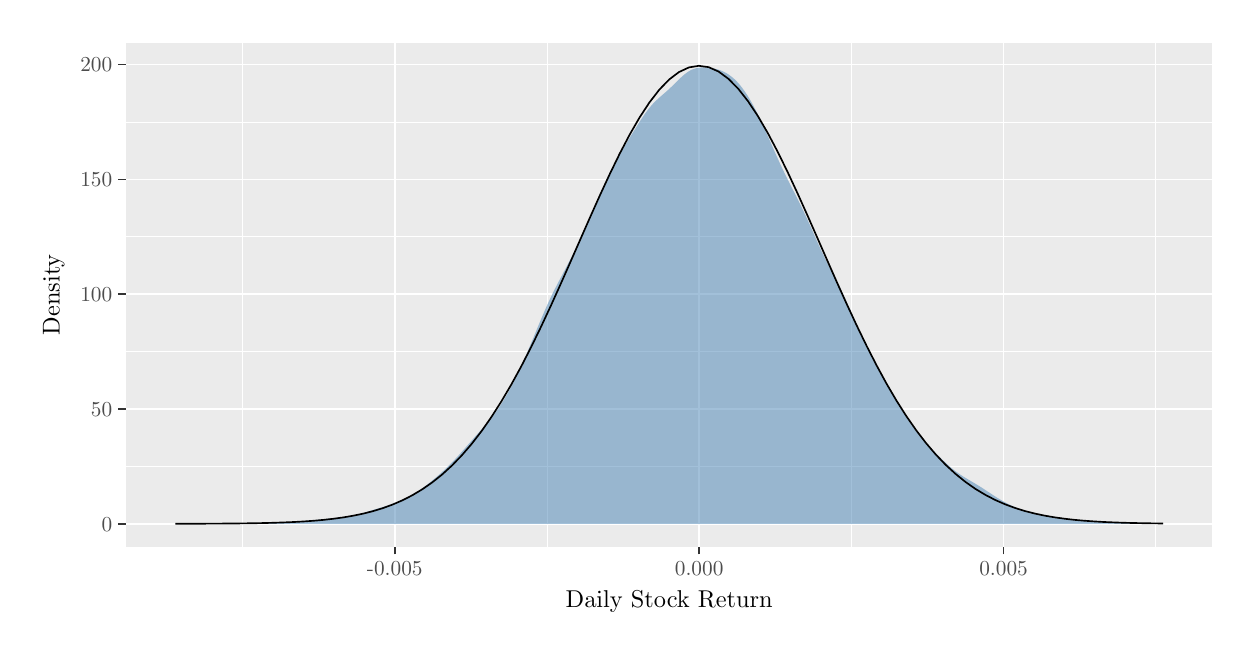
\begin{tikzpicture}[x=1pt,y=1pt]
\definecolor{fillColor}{RGB}{255,255,255}
\path[use as bounding box,fill=fillColor,fill opacity=0.00] (0,0) rectangle (433.62,216.81);
\begin{scope}
\path[clip] (  0.00,  0.00) rectangle (433.62,216.81);
\definecolor{drawColor}{RGB}{255,255,255}
\definecolor{fillColor}{RGB}{255,255,255}

\path[draw=drawColor,line width= 0.6pt,line join=round,line cap=round,fill=fillColor] (  0.00,  0.00) rectangle (433.62,216.81);
\end{scope}
\begin{scope}
\path[clip] ( 35.50, 29.26) rectangle (428.12,211.31);
\definecolor{fillColor}{gray}{0.92}

\path[fill=fillColor] ( 35.50, 29.26) rectangle (428.12,211.31);
\definecolor{drawColor}{RGB}{255,255,255}

\path[draw=drawColor,line width= 0.3pt,line join=round] ( 35.50, 58.28) --
	(428.12, 58.28);

\path[draw=drawColor,line width= 0.3pt,line join=round] ( 35.50, 99.76) --
	(428.12, 99.76);

\path[draw=drawColor,line width= 0.3pt,line join=round] ( 35.50,141.25) --
	(428.12,141.25);

\path[draw=drawColor,line width= 0.3pt,line join=round] ( 35.50,182.73) --
	(428.12,182.73);

\path[draw=drawColor,line width= 0.3pt,line join=round] ( 77.67, 29.26) --
	( 77.67,211.31);

\path[draw=drawColor,line width= 0.3pt,line join=round] (187.65, 29.26) --
	(187.65,211.31);

\path[draw=drawColor,line width= 0.3pt,line join=round] (297.64, 29.26) --
	(297.64,211.31);

\path[draw=drawColor,line width= 0.3pt,line join=round] (407.62, 29.26) --
	(407.62,211.31);

\path[draw=drawColor,line width= 0.6pt,line join=round] ( 35.50, 37.53) --
	(428.12, 37.53);

\path[draw=drawColor,line width= 0.6pt,line join=round] ( 35.50, 79.02) --
	(428.12, 79.02);

\path[draw=drawColor,line width= 0.6pt,line join=round] ( 35.50,120.50) --
	(428.12,120.50);

\path[draw=drawColor,line width= 0.6pt,line join=round] ( 35.50,161.99) --
	(428.12,161.99);

\path[draw=drawColor,line width= 0.6pt,line join=round] ( 35.50,203.47) --
	(428.12,203.47);

\path[draw=drawColor,line width= 0.6pt,line join=round] (132.66, 29.26) --
	(132.66,211.31);

\path[draw=drawColor,line width= 0.6pt,line join=round] (242.64, 29.26) --
	(242.64,211.31);

\path[draw=drawColor,line width= 0.6pt,line join=round] (352.63, 29.26) --
	(352.63,211.31);
\definecolor{fillColor}{RGB}{70,130,180}

\path[fill=fillColor,fill opacity=0.50] ( 53.35, 37.57) --
	( 54.05, 37.57) --
	( 54.75, 37.57) --
	( 55.44, 37.57) --
	( 56.14, 37.57) --
	( 56.84, 37.56) --
	( 57.54, 37.56) --
	( 58.24, 37.56) --
	( 58.94, 37.55) --
	( 59.63, 37.55) --
	( 60.33, 37.55) --
	( 61.03, 37.54) --
	( 61.73, 37.54) --
	( 62.43, 37.54) --
	( 63.13, 37.54) --
	( 63.83, 37.54) --
	( 64.52, 37.54) --
	( 65.22, 37.54) --
	( 65.92, 37.54) --
	( 66.62, 37.55) --
	( 67.32, 37.55) --
	( 68.02, 37.56) --
	( 68.71, 37.56) --
	( 69.41, 37.57) --
	( 70.11, 37.58) --
	( 70.81, 37.58) --
	( 71.51, 37.59) --
	( 72.21, 37.61) --
	( 72.91, 37.62) --
	( 73.60, 37.63) --
	( 74.30, 37.64) --
	( 75.00, 37.66) --
	( 75.70, 37.67) --
	( 76.40, 37.69) --
	( 77.10, 37.70) --
	( 77.80, 37.71) --
	( 78.49, 37.73) --
	( 79.19, 37.74) --
	( 79.89, 37.75) --
	( 80.59, 37.76) --
	( 81.29, 37.77) --
	( 81.99, 37.78) --
	( 82.68, 37.78) --
	( 83.38, 37.79) --
	( 84.08, 37.80) --
	( 84.78, 37.81) --
	( 85.48, 37.81) --
	( 86.18, 37.82) --
	( 86.88, 37.83) --
	( 87.57, 37.85) --
	( 88.27, 37.86) --
	( 88.97, 37.88) --
	( 89.67, 37.90) --
	( 90.37, 37.92) --
	( 91.07, 37.94) --
	( 91.76, 37.97) --
	( 92.46, 38.00) --
	( 93.16, 38.03) --
	( 93.86, 38.07) --
	( 94.56, 38.10) --
	( 95.26, 38.15) --
	( 95.96, 38.19) --
	( 96.65, 38.24) --
	( 97.35, 38.29) --
	( 98.05, 38.34) --
	( 98.75, 38.40) --
	( 99.45, 38.46) --
	(100.15, 38.52) --
	(100.85, 38.58) --
	(101.54, 38.64) --
	(102.24, 38.71) --
	(102.94, 38.77) --
	(103.64, 38.84) --
	(104.34, 38.91) --
	(105.04, 38.99) --
	(105.73, 39.06) --
	(106.43, 39.14) --
	(107.13, 39.22) --
	(107.83, 39.30) --
	(108.53, 39.38) --
	(109.23, 39.45) --
	(109.93, 39.53) --
	(110.62, 39.60) --
	(111.32, 39.67) --
	(112.02, 39.74) --
	(112.72, 39.81) --
	(113.42, 39.88) --
	(114.12, 39.95) --
	(114.81, 40.03) --
	(115.51, 40.12) --
	(116.21, 40.22) --
	(116.91, 40.33) --
	(117.61, 40.47) --
	(118.31, 40.61) --
	(119.01, 40.77) --
	(119.70, 40.95) --
	(120.40, 41.15) --
	(121.10, 41.35) --
	(121.80, 41.56) --
	(122.50, 41.78) --
	(123.20, 42.01) --
	(123.90, 42.23) --
	(124.59, 42.45) --
	(125.29, 42.67) --
	(125.99, 42.89) --
	(126.69, 43.10) --
	(127.39, 43.31) --
	(128.09, 43.51) --
	(128.78, 43.71) --
	(129.48, 43.92) --
	(130.18, 44.13) --
	(130.88, 44.35) --
	(131.58, 44.57) --
	(132.28, 44.81) --
	(132.98, 45.06) --
	(133.67, 45.33) --
	(134.37, 45.61) --
	(135.07, 45.91) --
	(135.77, 46.22) --
	(136.47, 46.56) --
	(137.17, 46.91) --
	(137.86, 47.29) --
	(138.56, 47.69) --
	(139.26, 48.11) --
	(139.96, 48.54) --
	(140.66, 49.00) --
	(141.36, 49.48) --
	(142.06, 49.97) --
	(142.75, 50.48) --
	(143.45, 51.00) --
	(144.15, 51.53) --
	(144.85, 52.08) --
	(145.55, 52.64) --
	(146.25, 53.21) --
	(146.95, 53.78) --
	(147.64, 54.37) --
	(148.34, 54.98) --
	(149.04, 55.59) --
	(149.74, 56.22) --
	(150.44, 56.86) --
	(151.14, 57.52) --
	(151.83, 58.20) --
	(152.53, 58.89) --
	(153.23, 59.60) --
	(153.93, 60.33) --
	(154.63, 61.08) --
	(155.33, 61.83) --
	(156.03, 62.60) --
	(156.72, 63.38) --
	(157.42, 64.17) --
	(158.12, 64.96) --
	(158.82, 65.76) --
	(159.52, 66.56) --
	(160.22, 67.36) --
	(160.91, 68.15) --
	(161.61, 68.95) --
	(162.31, 69.74) --
	(163.01, 70.52) --
	(163.71, 71.31) --
	(164.41, 72.10) --
	(165.11, 72.90) --
	(165.80, 73.70) --
	(166.50, 74.52) --
	(167.20, 75.37) --
	(167.90, 76.25) --
	(168.60, 77.16) --
	(169.30, 78.11) --
	(170.00, 79.10) --
	(170.69, 80.15) --
	(171.39, 81.24) --
	(172.09, 82.37) --
	(172.79, 83.56) --
	(173.49, 84.80) --
	(174.19, 86.09) --
	(174.88, 87.42) --
	(175.58, 88.80) --
	(176.28, 90.21) --
	(176.98, 91.66) --
	(177.68, 93.15) --
	(178.38, 94.66) --
	(179.08, 96.21) --
	(179.77, 97.79) --
	(180.47, 99.40) --
	(181.17,101.03) --
	(181.87,102.68) --
	(182.57,104.35) --
	(183.27,106.04) --
	(183.96,107.73) --
	(184.66,109.42) --
	(185.36,111.10) --
	(186.06,112.75) --
	(186.76,114.38) --
	(187.46,115.97) --
	(188.16,117.52) --
	(188.85,119.02) --
	(189.55,120.48) --
	(190.25,121.89) --
	(190.95,123.27) --
	(191.65,124.62) --
	(192.35,125.95) --
	(193.05,127.27) --
	(193.74,128.59) --
	(194.44,129.92) --
	(195.14,131.25) --
	(195.84,132.60) --
	(196.54,133.96) --
	(197.24,135.35) --
	(197.93,136.75) --
	(198.63,138.18) --
	(199.33,139.62) --
	(200.03,141.09) --
	(200.73,142.59) --
	(201.43,144.11) --
	(202.13,145.65) --
	(202.82,147.23) --
	(203.52,148.83) --
	(204.22,150.45) --
	(204.92,152.09) --
	(205.62,153.74) --
	(206.32,155.38) --
	(207.01,157.02) --
	(207.71,158.63) --
	(208.41,160.22) --
	(209.11,161.76) --
	(209.81,163.27) --
	(210.51,164.72) --
	(211.21,166.11) --
	(211.90,167.46) --
	(212.60,168.75) --
	(213.30,170.00) --
	(214.00,171.22) --
	(214.70,172.40) --
	(215.40,173.56) --
	(216.10,174.70) --
	(216.79,175.84) --
	(217.49,176.97) --
	(218.19,178.10) --
	(218.89,179.22) --
	(219.59,180.35) --
	(220.29,181.47) --
	(220.98,182.57) --
	(221.68,183.65) --
	(222.38,184.71) --
	(223.08,185.72) --
	(223.78,186.69) --
	(224.48,187.60) --
	(225.18,188.44) --
	(225.87,189.23) --
	(226.57,189.96) --
	(227.27,190.64) --
	(227.97,191.29) --
	(228.67,191.90) --
	(229.37,192.51) --
	(230.06,193.11) --
	(230.76,193.72) --
	(231.46,194.34) --
	(232.16,194.99) --
	(232.86,195.66) --
	(233.56,196.34) --
	(234.26,197.04) --
	(234.95,197.73) --
	(235.65,198.41) --
	(236.35,199.06) --
	(237.05,199.67) --
	(237.75,200.24) --
	(238.45,200.75) --
	(239.15,201.19) --
	(239.84,201.56) --
	(240.54,201.85) --
	(241.24,202.08) --
	(241.94,202.25) --
	(242.64,202.36) --
	(243.34,202.42) --
	(244.03,202.44) --
	(244.73,202.43) --
	(245.43,202.39) --
	(246.13,202.32) --
	(246.83,202.24) --
	(247.53,202.12) --
	(248.23,201.99) --
	(248.92,201.82) --
	(249.62,201.62) --
	(250.32,201.38) --
	(251.02,201.11) --
	(251.72,200.78) --
	(252.42,200.41) --
	(253.11,199.99) --
	(253.81,199.50) --
	(254.51,198.96) --
	(255.21,198.36) --
	(255.91,197.69) --
	(256.61,196.96) --
	(257.31,196.16) --
	(258.00,195.29) --
	(258.70,194.35) --
	(259.40,193.35) --
	(260.10,192.28) --
	(260.80,191.14) --
	(261.50,189.94) --
	(262.20,188.68) --
	(262.89,187.36) --
	(263.59,185.99) --
	(264.29,184.57) --
	(264.99,183.10) --
	(265.69,181.60) --
	(266.39,180.05) --
	(267.08,178.49) --
	(267.78,176.90) --
	(268.48,175.30) --
	(269.18,173.70) --
	(269.88,172.11) --
	(270.58,170.53) --
	(271.28,168.98) --
	(271.97,167.45) --
	(272.67,165.96) --
	(273.37,164.50) --
	(274.07,163.07) --
	(274.77,161.66) --
	(275.47,160.27) --
	(276.16,158.90) --
	(276.86,157.53) --
	(277.56,156.16) --
	(278.26,154.77) --
	(278.96,153.37) --
	(279.66,151.94) --
	(280.36,150.48) --
	(281.05,148.99) --
	(281.75,147.47) --
	(282.45,145.93) --
	(283.15,144.36) --
	(283.85,142.78) --
	(284.55,141.20) --
	(285.25,139.62) --
	(285.94,138.07) --
	(286.64,136.55) --
	(287.34,135.06) --
	(288.04,133.61) --
	(288.74,132.19) --
	(289.44,130.81) --
	(290.13,129.45) --
	(290.83,128.11) --
	(291.53,126.76) --
	(292.23,125.41) --
	(292.93,124.03) --
	(293.63,122.63) --
	(294.33,121.18) --
	(295.02,119.70) --
	(295.72,118.17) --
	(296.42,116.62) --
	(297.12,115.03) --
	(297.82,113.42) --
	(298.52,111.80) --
	(299.21,110.18) --
	(299.91,108.58) --
	(300.61,106.99) --
	(301.31,105.43) --
	(302.01,103.90) --
	(302.71,102.40) --
	(303.41,100.94) --
	(304.10, 99.52) --
	(304.80, 98.13) --
	(305.50, 96.78) --
	(306.20, 95.46) --
	(306.90, 94.17) --
	(307.60, 92.90) --
	(308.30, 91.65) --
	(308.99, 90.41) --
	(309.69, 89.19) --
	(310.39, 87.98) --
	(311.09, 86.78) --
	(311.79, 85.58) --
	(312.49, 84.39) --
	(313.18, 83.20) --
	(313.88, 82.01) --
	(314.58, 80.84) --
	(315.28, 79.67) --
	(315.98, 78.52) --
	(316.68, 77.38) --
	(317.38, 76.26) --
	(318.07, 75.18) --
	(318.77, 74.12) --
	(319.47, 73.10) --
	(320.17, 72.12) --
	(320.87, 71.18) --
	(321.57, 70.28) --
	(322.26, 69.41) --
	(322.96, 68.58) --
	(323.66, 67.78) --
	(324.36, 67.01) --
	(325.06, 66.25) --
	(325.76, 65.51) --
	(326.46, 64.79) --
	(327.15, 64.07) --
	(327.85, 63.36) --
	(328.55, 62.66) --
	(329.25, 61.96) --
	(329.95, 61.27) --
	(330.65, 60.58) --
	(331.35, 59.91) --
	(332.04, 59.26) --
	(332.74, 58.62) --
	(333.44, 58.01) --
	(334.14, 57.42) --
	(334.84, 56.86) --
	(335.54, 56.33) --
	(336.23, 55.83) --
	(336.93, 55.35) --
	(337.63, 54.89) --
	(338.33, 54.46) --
	(339.03, 54.03) --
	(339.73, 53.62) --
	(340.43, 53.21) --
	(341.12, 52.80) --
	(341.82, 52.39) --
	(342.52, 51.97) --
	(343.22, 51.55) --
	(343.92, 51.12) --
	(344.62, 50.68) --
	(345.31, 50.23) --
	(346.01, 49.77) --
	(346.71, 49.31) --
	(347.41, 48.85) --
	(348.11, 48.39) --
	(348.81, 47.93) --
	(349.51, 47.48) --
	(350.20, 47.04) --
	(350.90, 46.60) --
	(351.60, 46.18) --
	(352.30, 45.78) --
	(353.00, 45.38) --
	(353.70, 45.01) --
	(354.39, 44.65) --
	(355.09, 44.31) --
	(355.79, 43.98) --
	(356.49, 43.67) --
	(357.19, 43.37) --
	(357.89, 43.09) --
	(358.59, 42.82) --
	(359.28, 42.56) --
	(359.98, 42.32) --
	(360.68, 42.10) --
	(361.38, 41.88) --
	(362.08, 41.68) --
	(362.78, 41.50) --
	(363.48, 41.32) --
	(364.17, 41.16) --
	(364.87, 41.01) --
	(365.57, 40.86) --
	(366.27, 40.73) --
	(366.97, 40.60) --
	(367.67, 40.48) --
	(368.36, 40.36) --
	(369.06, 40.25) --
	(369.76, 40.15) --
	(370.46, 40.05) --
	(371.16, 39.95) --
	(371.86, 39.85) --
	(372.56, 39.76) --
	(373.25, 39.67) --
	(373.95, 39.58) --
	(374.65, 39.49) --
	(375.35, 39.40) --
	(376.05, 39.32) --
	(376.75, 39.23) --
	(377.44, 39.15) --
	(378.14, 39.06) --
	(378.84, 38.98) --
	(379.54, 38.90) --
	(380.24, 38.82) --
	(380.94, 38.74) --
	(381.64, 38.66) --
	(382.33, 38.59) --
	(383.03, 38.53) --
	(383.73, 38.46) --
	(384.43, 38.40) --
	(385.13, 38.35) --
	(385.83, 38.29) --
	(386.53, 38.25) --
	(387.22, 38.20) --
	(387.92, 38.16) --
	(388.62, 38.12) --
	(389.32, 38.08) --
	(390.02, 38.04) --
	(390.72, 38.01) --
	(391.41, 37.98) --
	(392.11, 37.95) --
	(392.81, 37.93) --
	(393.51, 37.90) --
	(394.21, 37.89) --
	(394.91, 37.87) --
	(395.61, 37.86) --
	(396.30, 37.85) --
	(397.00, 37.84) --
	(397.70, 37.84) --
	(398.40, 37.83) --
	(399.10, 37.83) --
	(399.80, 37.83) --
	(400.49, 37.83) --
	(401.19, 37.83) --
	(401.89, 37.83) --
	(402.59, 37.82) --
	(403.29, 37.82) --
	(403.99, 37.81) --
	(404.69, 37.80) --
	(405.38, 37.79) --
	(406.08, 37.78) --
	(406.78, 37.76) --
	(407.48, 37.75) --
	(408.18, 37.73) --
	(408.88, 37.72) --
	(409.58, 37.70) --
	(410.27, 37.69) --
	(410.27, 37.53) --
	(409.58, 37.53) --
	(408.88, 37.53) --
	(408.18, 37.53) --
	(407.48, 37.53) --
	(406.78, 37.53) --
	(406.08, 37.53) --
	(405.38, 37.53) --
	(404.69, 37.53) --
	(403.99, 37.53) --
	(403.29, 37.53) --
	(402.59, 37.53) --
	(401.89, 37.53) --
	(401.19, 37.53) --
	(400.49, 37.53) --
	(399.80, 37.53) --
	(399.10, 37.53) --
	(398.40, 37.53) --
	(397.70, 37.53) --
	(397.00, 37.53) --
	(396.30, 37.53) --
	(395.61, 37.53) --
	(394.91, 37.53) --
	(394.21, 37.53) --
	(393.51, 37.53) --
	(392.81, 37.53) --
	(392.11, 37.53) --
	(391.41, 37.53) --
	(390.72, 37.53) --
	(390.02, 37.53) --
	(389.32, 37.53) --
	(388.62, 37.53) --
	(387.92, 37.53) --
	(387.22, 37.53) --
	(386.53, 37.53) --
	(385.83, 37.53) --
	(385.13, 37.53) --
	(384.43, 37.53) --
	(383.73, 37.53) --
	(383.03, 37.53) --
	(382.33, 37.53) --
	(381.64, 37.53) --
	(380.94, 37.53) --
	(380.24, 37.53) --
	(379.54, 37.53) --
	(378.84, 37.53) --
	(378.14, 37.53) --
	(377.44, 37.53) --
	(376.75, 37.53) --
	(376.05, 37.53) --
	(375.35, 37.53) --
	(374.65, 37.53) --
	(373.95, 37.53) --
	(373.25, 37.53) --
	(372.56, 37.53) --
	(371.86, 37.53) --
	(371.16, 37.53) --
	(370.46, 37.53) --
	(369.76, 37.53) --
	(369.06, 37.53) --
	(368.36, 37.53) --
	(367.67, 37.53) --
	(366.97, 37.53) --
	(366.27, 37.53) --
	(365.57, 37.53) --
	(364.87, 37.53) --
	(364.17, 37.53) --
	(363.48, 37.53) --
	(362.78, 37.53) --
	(362.08, 37.53) --
	(361.38, 37.53) --
	(360.68, 37.53) --
	(359.98, 37.53) --
	(359.28, 37.53) --
	(358.59, 37.53) --
	(357.89, 37.53) --
	(357.19, 37.53) --
	(356.49, 37.53) --
	(355.79, 37.53) --
	(355.09, 37.53) --
	(354.39, 37.53) --
	(353.70, 37.53) --
	(353.00, 37.53) --
	(352.30, 37.53) --
	(351.60, 37.53) --
	(350.90, 37.53) --
	(350.20, 37.53) --
	(349.51, 37.53) --
	(348.81, 37.53) --
	(348.11, 37.53) --
	(347.41, 37.53) --
	(346.71, 37.53) --
	(346.01, 37.53) --
	(345.31, 37.53) --
	(344.62, 37.53) --
	(343.92, 37.53) --
	(343.22, 37.53) --
	(342.52, 37.53) --
	(341.82, 37.53) --
	(341.12, 37.53) --
	(340.43, 37.53) --
	(339.73, 37.53) --
	(339.03, 37.53) --
	(338.33, 37.53) --
	(337.63, 37.53) --
	(336.93, 37.53) --
	(336.23, 37.53) --
	(335.54, 37.53) --
	(334.84, 37.53) --
	(334.14, 37.53) --
	(333.44, 37.53) --
	(332.74, 37.53) --
	(332.04, 37.53) --
	(331.35, 37.53) --
	(330.65, 37.53) --
	(329.95, 37.53) --
	(329.25, 37.53) --
	(328.55, 37.53) --
	(327.85, 37.53) --
	(327.15, 37.53) --
	(326.46, 37.53) --
	(325.76, 37.53) --
	(325.06, 37.53) --
	(324.36, 37.53) --
	(323.66, 37.53) --
	(322.96, 37.53) --
	(322.26, 37.53) --
	(321.57, 37.53) --
	(320.87, 37.53) --
	(320.17, 37.53) --
	(319.47, 37.53) --
	(318.77, 37.53) --
	(318.07, 37.53) --
	(317.38, 37.53) --
	(316.68, 37.53) --
	(315.98, 37.53) --
	(315.28, 37.53) --
	(314.58, 37.53) --
	(313.88, 37.53) --
	(313.18, 37.53) --
	(312.49, 37.53) --
	(311.79, 37.53) --
	(311.09, 37.53) --
	(310.39, 37.53) --
	(309.69, 37.53) --
	(308.99, 37.53) --
	(308.30, 37.53) --
	(307.60, 37.53) --
	(306.90, 37.53) --
	(306.20, 37.53) --
	(305.50, 37.53) --
	(304.80, 37.53) --
	(304.10, 37.53) --
	(303.41, 37.53) --
	(302.71, 37.53) --
	(302.01, 37.53) --
	(301.31, 37.53) --
	(300.61, 37.53) --
	(299.91, 37.53) --
	(299.21, 37.53) --
	(298.52, 37.53) --
	(297.82, 37.53) --
	(297.12, 37.53) --
	(296.42, 37.53) --
	(295.72, 37.53) --
	(295.02, 37.53) --
	(294.33, 37.53) --
	(293.63, 37.53) --
	(292.93, 37.53) --
	(292.23, 37.53) --
	(291.53, 37.53) --
	(290.83, 37.53) --
	(290.13, 37.53) --
	(289.44, 37.53) --
	(288.74, 37.53) --
	(288.04, 37.53) --
	(287.34, 37.53) --
	(286.64, 37.53) --
	(285.94, 37.53) --
	(285.25, 37.53) --
	(284.55, 37.53) --
	(283.85, 37.53) --
	(283.15, 37.53) --
	(282.45, 37.53) --
	(281.75, 37.53) --
	(281.05, 37.53) --
	(280.36, 37.53) --
	(279.66, 37.53) --
	(278.96, 37.53) --
	(278.26, 37.53) --
	(277.56, 37.53) --
	(276.86, 37.53) --
	(276.16, 37.53) --
	(275.47, 37.53) --
	(274.77, 37.53) --
	(274.07, 37.53) --
	(273.37, 37.53) --
	(272.67, 37.53) --
	(271.97, 37.53) --
	(271.28, 37.53) --
	(270.58, 37.53) --
	(269.88, 37.53) --
	(269.18, 37.53) --
	(268.48, 37.53) --
	(267.78, 37.53) --
	(267.08, 37.53) --
	(266.39, 37.53) --
	(265.69, 37.53) --
	(264.99, 37.53) --
	(264.29, 37.53) --
	(263.59, 37.53) --
	(262.89, 37.53) --
	(262.20, 37.53) --
	(261.50, 37.53) --
	(260.80, 37.53) --
	(260.10, 37.53) --
	(259.40, 37.53) --
	(258.70, 37.53) --
	(258.00, 37.53) --
	(257.31, 37.53) --
	(256.61, 37.53) --
	(255.91, 37.53) --
	(255.21, 37.53) --
	(254.51, 37.53) --
	(253.81, 37.53) --
	(253.11, 37.53) --
	(252.42, 37.53) --
	(251.72, 37.53) --
	(251.02, 37.53) --
	(250.32, 37.53) --
	(249.62, 37.53) --
	(248.92, 37.53) --
	(248.23, 37.53) --
	(247.53, 37.53) --
	(246.83, 37.53) --
	(246.13, 37.53) --
	(245.43, 37.53) --
	(244.73, 37.53) --
	(244.03, 37.53) --
	(243.34, 37.53) --
	(242.64, 37.53) --
	(241.94, 37.53) --
	(241.24, 37.53) --
	(240.54, 37.53) --
	(239.84, 37.53) --
	(239.15, 37.53) --
	(238.45, 37.53) --
	(237.75, 37.53) --
	(237.05, 37.53) --
	(236.35, 37.53) --
	(235.65, 37.53) --
	(234.95, 37.53) --
	(234.26, 37.53) --
	(233.56, 37.53) --
	(232.86, 37.53) --
	(232.16, 37.53) --
	(231.46, 37.53) --
	(230.76, 37.53) --
	(230.06, 37.53) --
	(229.37, 37.53) --
	(228.67, 37.53) --
	(227.97, 37.53) --
	(227.27, 37.53) --
	(226.57, 37.53) --
	(225.87, 37.53) --
	(225.18, 37.53) --
	(224.48, 37.53) --
	(223.78, 37.53) --
	(223.08, 37.53) --
	(222.38, 37.53) --
	(221.68, 37.53) --
	(220.98, 37.53) --
	(220.29, 37.53) --
	(219.59, 37.53) --
	(218.89, 37.53) --
	(218.19, 37.53) --
	(217.49, 37.53) --
	(216.79, 37.53) --
	(216.10, 37.53) --
	(215.40, 37.53) --
	(214.70, 37.53) --
	(214.00, 37.53) --
	(213.30, 37.53) --
	(212.60, 37.53) --
	(211.90, 37.53) --
	(211.21, 37.53) --
	(210.51, 37.53) --
	(209.81, 37.53) --
	(209.11, 37.53) --
	(208.41, 37.53) --
	(207.71, 37.53) --
	(207.01, 37.53) --
	(206.32, 37.53) --
	(205.62, 37.53) --
	(204.92, 37.53) --
	(204.22, 37.53) --
	(203.52, 37.53) --
	(202.82, 37.53) --
	(202.13, 37.53) --
	(201.43, 37.53) --
	(200.73, 37.53) --
	(200.03, 37.53) --
	(199.33, 37.53) --
	(198.63, 37.53) --
	(197.93, 37.53) --
	(197.24, 37.53) --
	(196.54, 37.53) --
	(195.84, 37.53) --
	(195.14, 37.53) --
	(194.44, 37.53) --
	(193.74, 37.53) --
	(193.05, 37.53) --
	(192.35, 37.53) --
	(191.65, 37.53) --
	(190.95, 37.53) --
	(190.25, 37.53) --
	(189.55, 37.53) --
	(188.85, 37.53) --
	(188.16, 37.53) --
	(187.46, 37.53) --
	(186.76, 37.53) --
	(186.06, 37.53) --
	(185.36, 37.53) --
	(184.66, 37.53) --
	(183.96, 37.53) --
	(183.27, 37.53) --
	(182.57, 37.53) --
	(181.87, 37.53) --
	(181.17, 37.53) --
	(180.47, 37.53) --
	(179.77, 37.53) --
	(179.08, 37.53) --
	(178.38, 37.53) --
	(177.68, 37.53) --
	(176.98, 37.53) --
	(176.28, 37.53) --
	(175.58, 37.53) --
	(174.88, 37.53) --
	(174.19, 37.53) --
	(173.49, 37.53) --
	(172.79, 37.53) --
	(172.09, 37.53) --
	(171.39, 37.53) --
	(170.69, 37.53) --
	(170.00, 37.53) --
	(169.30, 37.53) --
	(168.60, 37.53) --
	(167.90, 37.53) --
	(167.20, 37.53) --
	(166.50, 37.53) --
	(165.80, 37.53) --
	(165.11, 37.53) --
	(164.41, 37.53) --
	(163.71, 37.53) --
	(163.01, 37.53) --
	(162.31, 37.53) --
	(161.61, 37.53) --
	(160.91, 37.53) --
	(160.22, 37.53) --
	(159.52, 37.53) --
	(158.82, 37.53) --
	(158.12, 37.53) --
	(157.42, 37.53) --
	(156.72, 37.53) --
	(156.03, 37.53) --
	(155.33, 37.53) --
	(154.63, 37.53) --
	(153.93, 37.53) --
	(153.23, 37.53) --
	(152.53, 37.53) --
	(151.83, 37.53) --
	(151.14, 37.53) --
	(150.44, 37.53) --
	(149.74, 37.53) --
	(149.04, 37.53) --
	(148.34, 37.53) --
	(147.64, 37.53) --
	(146.95, 37.53) --
	(146.25, 37.53) --
	(145.55, 37.53) --
	(144.85, 37.53) --
	(144.15, 37.53) --
	(143.45, 37.53) --
	(142.75, 37.53) --
	(142.06, 37.53) --
	(141.36, 37.53) --
	(140.66, 37.53) --
	(139.96, 37.53) --
	(139.26, 37.53) --
	(138.56, 37.53) --
	(137.86, 37.53) --
	(137.17, 37.53) --
	(136.47, 37.53) --
	(135.77, 37.53) --
	(135.07, 37.53) --
	(134.37, 37.53) --
	(133.67, 37.53) --
	(132.98, 37.53) --
	(132.28, 37.53) --
	(131.58, 37.53) --
	(130.88, 37.53) --
	(130.18, 37.53) --
	(129.48, 37.53) --
	(128.78, 37.53) --
	(128.09, 37.53) --
	(127.39, 37.53) --
	(126.69, 37.53) --
	(125.99, 37.53) --
	(125.29, 37.53) --
	(124.59, 37.53) --
	(123.90, 37.53) --
	(123.20, 37.53) --
	(122.50, 37.53) --
	(121.80, 37.53) --
	(121.10, 37.53) --
	(120.40, 37.53) --
	(119.70, 37.53) --
	(119.01, 37.53) --
	(118.31, 37.53) --
	(117.61, 37.53) --
	(116.91, 37.53) --
	(116.21, 37.53) --
	(115.51, 37.53) --
	(114.81, 37.53) --
	(114.12, 37.53) --
	(113.42, 37.53) --
	(112.72, 37.53) --
	(112.02, 37.53) --
	(111.32, 37.53) --
	(110.62, 37.53) --
	(109.93, 37.53) --
	(109.23, 37.53) --
	(108.53, 37.53) --
	(107.83, 37.53) --
	(107.13, 37.53) --
	(106.43, 37.53) --
	(105.73, 37.53) --
	(105.04, 37.53) --
	(104.34, 37.53) --
	(103.64, 37.53) --
	(102.94, 37.53) --
	(102.24, 37.53) --
	(101.54, 37.53) --
	(100.85, 37.53) --
	(100.15, 37.53) --
	( 99.45, 37.53) --
	( 98.75, 37.53) --
	( 98.05, 37.53) --
	( 97.35, 37.53) --
	( 96.65, 37.53) --
	( 95.96, 37.53) --
	( 95.26, 37.53) --
	( 94.56, 37.53) --
	( 93.86, 37.53) --
	( 93.16, 37.53) --
	( 92.46, 37.53) --
	( 91.76, 37.53) --
	( 91.07, 37.53) --
	( 90.37, 37.53) --
	( 89.67, 37.53) --
	( 88.97, 37.53) --
	( 88.27, 37.53) --
	( 87.57, 37.53) --
	( 86.88, 37.53) --
	( 86.18, 37.53) --
	( 85.48, 37.53) --
	( 84.78, 37.53) --
	( 84.08, 37.53) --
	( 83.38, 37.53) --
	( 82.68, 37.53) --
	( 81.99, 37.53) --
	( 81.29, 37.53) --
	( 80.59, 37.53) --
	( 79.89, 37.53) --
	( 79.19, 37.53) --
	( 78.49, 37.53) --
	( 77.80, 37.53) --
	( 77.10, 37.53) --
	( 76.40, 37.53) --
	( 75.70, 37.53) --
	( 75.00, 37.53) --
	( 74.30, 37.53) --
	( 73.60, 37.53) --
	( 72.91, 37.53) --
	( 72.21, 37.53) --
	( 71.51, 37.53) --
	( 70.81, 37.53) --
	( 70.11, 37.53) --
	( 69.41, 37.53) --
	( 68.71, 37.53) --
	( 68.02, 37.53) --
	( 67.32, 37.53) --
	( 66.62, 37.53) --
	( 65.92, 37.53) --
	( 65.22, 37.53) --
	( 64.52, 37.53) --
	( 63.83, 37.53) --
	( 63.13, 37.53) --
	( 62.43, 37.53) --
	( 61.73, 37.53) --
	( 61.03, 37.53) --
	( 60.33, 37.53) --
	( 59.63, 37.53) --
	( 58.94, 37.53) --
	( 58.24, 37.53) --
	( 57.54, 37.53) --
	( 56.84, 37.53) --
	( 56.14, 37.53) --
	( 55.44, 37.53) --
	( 54.75, 37.53) --
	( 54.05, 37.53) --
	( 53.35, 37.53) --
	cycle;
\definecolor{drawColor}{RGB}{0,0,0}

\path[draw=drawColor,line width= 0.6pt,line join=round] ( 53.35, 37.55) --
	( 56.92, 37.56) --
	( 60.49, 37.56) --
	( 64.06, 37.58) --
	( 67.63, 37.59) --
	( 71.19, 37.62) --
	( 74.76, 37.65) --
	( 78.33, 37.69) --
	( 81.90, 37.74) --
	( 85.47, 37.81) --
	( 89.04, 37.91) --
	( 92.61, 38.03) --
	( 96.18, 38.18) --
	( 99.75, 38.38) --
	(103.32, 38.63) --
	(106.89, 38.95) --
	(110.46, 39.35) --
	(114.03, 39.84) --
	(117.59, 40.45) --
	(121.16, 41.19) --
	(124.73, 42.09) --
	(128.30, 43.18) --
	(131.87, 44.49) --
	(135.44, 46.03) --
	(139.01, 47.86) --
	(142.58, 49.99) --
	(146.15, 52.47) --
	(149.72, 55.31) --
	(153.29, 58.57) --
	(156.86, 62.26) --
	(160.43, 66.40) --
	(164.00, 71.01) --
	(167.56, 76.11) --
	(171.13, 81.70) --
	(174.70, 87.76) --
	(178.27, 94.27) --
	(181.84,101.22) --
	(185.41,108.54) --
	(188.98,116.18) --
	(192.55,124.08) --
	(196.12,132.14) --
	(199.69,140.28) --
	(203.26,148.39) --
	(206.83,156.35) --
	(210.40,164.04) --
	(213.96,171.35) --
	(217.53,178.16) --
	(221.10,184.34) --
	(224.67,189.79) --
	(228.24,194.40) --
	(231.81,198.09) --
	(235.38,200.79) --
	(238.95,202.45) --
	(242.52,203.03) --
	(246.09,202.53) --
	(249.66,200.95) --
	(253.23,198.32) --
	(256.80,194.69) --
	(260.37,190.14) --
	(263.93,184.75) --
	(267.50,178.62) --
	(271.07,171.85) --
	(274.64,164.57) --
	(278.21,156.90) --
	(281.78,148.95) --
	(285.35,140.86) --
	(288.92,132.72) --
	(292.49,124.64) --
	(296.06,116.73) --
	(299.63,109.07) --
	(303.20,101.72) --
	(306.77, 94.75) --
	(310.33, 88.20) --
	(313.90, 82.11) --
	(317.47, 76.49) --
	(321.04, 71.36) --
	(324.61, 66.71) --
	(328.18, 62.53) --
	(331.75, 58.81) --
	(335.32, 55.53) --
	(338.89, 52.65) --
	(342.46, 50.15) --
	(346.03, 48.00) --
	(349.60, 46.15) --
	(353.17, 44.59) --
	(356.73, 43.27) --
	(360.30, 42.16) --
	(363.87, 41.25) --
	(367.44, 40.49) --
	(371.01, 39.88) --
	(374.58, 39.38) --
	(378.15, 38.97) --
	(381.72, 38.65) --
	(385.29, 38.40) --
	(388.86, 38.19) --
	(392.43, 38.04) --
	(396.00, 37.91) --
	(399.57, 37.82) --
	(403.14, 37.75) --
	(406.70, 37.69) --
	(410.27, 37.65);
\end{scope}
\begin{scope}
\path[clip] (  0.00,  0.00) rectangle (433.62,216.81);
\definecolor{drawColor}{gray}{0.30}

\node[text=drawColor,anchor=base east,inner sep=0pt, outer sep=0pt, scale=  0.77] at ( 30.55, 34.88) {0};

\node[text=drawColor,anchor=base east,inner sep=0pt, outer sep=0pt, scale=  0.77] at ( 30.55, 76.37) {50};

\node[text=drawColor,anchor=base east,inner sep=0pt, outer sep=0pt, scale=  0.77] at ( 30.55,117.85) {100};

\node[text=drawColor,anchor=base east,inner sep=0pt, outer sep=0pt, scale=  0.77] at ( 30.55,159.34) {150};

\node[text=drawColor,anchor=base east,inner sep=0pt, outer sep=0pt, scale=  0.77] at ( 30.55,200.82) {200};
\end{scope}
\begin{scope}
\path[clip] (  0.00,  0.00) rectangle (433.62,216.81);
\definecolor{drawColor}{gray}{0.20}

\path[draw=drawColor,line width= 0.6pt,line join=round] ( 32.75, 37.53) --
	( 35.50, 37.53);

\path[draw=drawColor,line width= 0.6pt,line join=round] ( 32.75, 79.02) --
	( 35.50, 79.02);

\path[draw=drawColor,line width= 0.6pt,line join=round] ( 32.75,120.50) --
	( 35.50,120.50);

\path[draw=drawColor,line width= 0.6pt,line join=round] ( 32.75,161.99) --
	( 35.50,161.99);

\path[draw=drawColor,line width= 0.6pt,line join=round] ( 32.75,203.47) --
	( 35.50,203.47);
\end{scope}
\begin{scope}
\path[clip] (  0.00,  0.00) rectangle (433.62,216.81);
\definecolor{drawColor}{gray}{0.20}

\path[draw=drawColor,line width= 0.6pt,line join=round] (132.66, 26.51) --
	(132.66, 29.26);

\path[draw=drawColor,line width= 0.6pt,line join=round] (242.64, 26.51) --
	(242.64, 29.26);

\path[draw=drawColor,line width= 0.6pt,line join=round] (352.63, 26.51) --
	(352.63, 29.26);
\end{scope}
\begin{scope}
\path[clip] (  0.00,  0.00) rectangle (433.62,216.81);
\definecolor{drawColor}{gray}{0.30}

\node[text=drawColor,anchor=base,inner sep=0pt, outer sep=0pt, scale=  0.77] at (132.66, 19.00) {-0.005};

\node[text=drawColor,anchor=base,inner sep=0pt, outer sep=0pt, scale=  0.77] at (242.64, 19.00) {0.000};

\node[text=drawColor,anchor=base,inner sep=0pt, outer sep=0pt, scale=  0.77] at (352.63, 19.00) {0.005};
\end{scope}
\begin{scope}
\path[clip] (  0.00,  0.00) rectangle (433.62,216.81);
\definecolor{drawColor}{RGB}{0,0,0}

\node[text=drawColor,anchor=base,inner sep=0pt, outer sep=0pt, scale=  0.88] at (231.81,  7.44) {Daily Stock Return};
\end{scope}
\begin{scope}
\path[clip] (  0.00,  0.00) rectangle (433.62,216.81);
\definecolor{drawColor}{RGB}{0,0,0}

\node[text=drawColor,rotate= 90.00,anchor=base,inner sep=0pt, outer sep=0pt, scale=  0.88] at ( 11.56,120.28) {Density};
\end{scope}
\end{tikzpicture}

\caption{Daily Basis Stock Return Density}
\label{p:returndensity}
\floatfoot{
The above density function has been constructed over 10000 samples of a unique process. The samples has been constructed following \cref{eq:Scontinuousdiffrate}. The arguments are set with the following value, $\alpha = 0$, $\sigma = 30\%$. The black density belongs to the normal bell curve with mean $\alpha$ and standard deviation of $\sigma \times \sqrt{dt}$. The period between each measure, namely $dt$ has been set to $10000^{-1}$. 
}
\end{figure}


%%%%%%%%%%%%%%%%%%%%%%%%%
%  Log-return
%%%%%%%%%%%%%%%%%%%%%%%%%

According to \cref{eq:underlyinglogreturn}, The distribution of the natural logarithm of the stock price return recorded over a time period of $t$ is characterized by \cref{eq:logreturndist}

\begin{center}
\begin{equation}
\ln{\frac{\St}{S\left(0\right)}} 
  \sim N((\alpha - \frac{\sigma^2}{2}) t, \sigma^2 t)
\label{eq:logreturndist}
\end{equation}
\end{center}  

\begin{figure}[!h]
\centering
% Created by tikzDevice version 0.11 on 2018-04-13 09:41:17
% !TEX encoding = UTF-8 Unicode
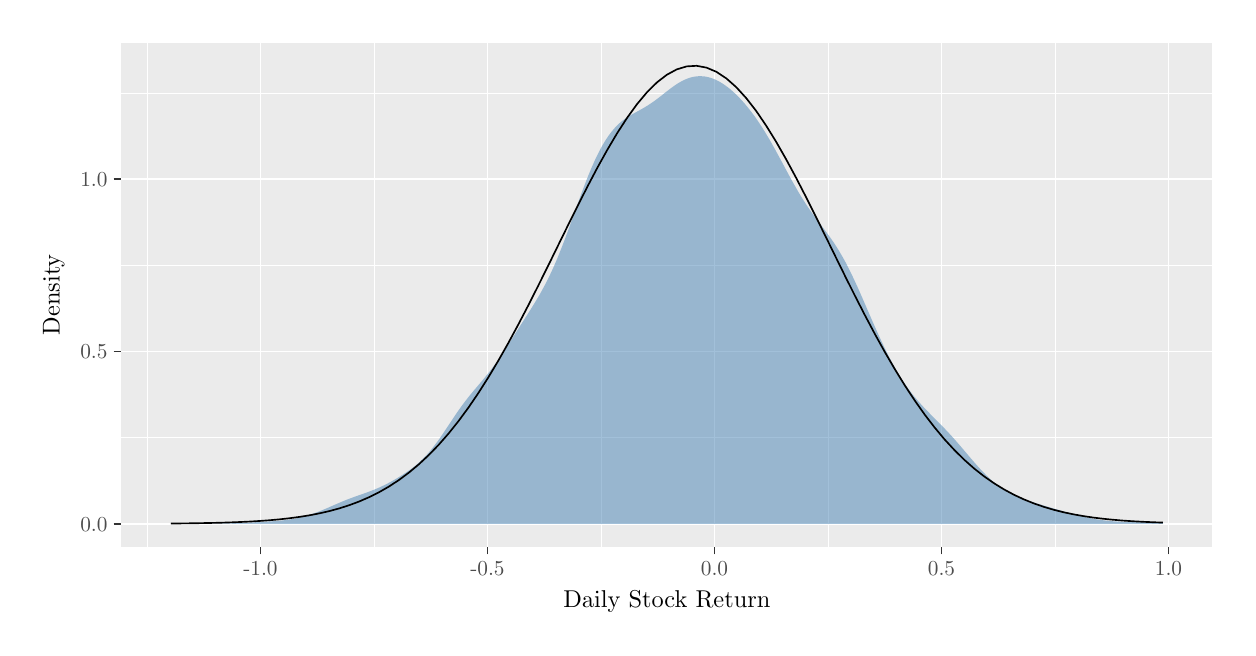
\begin{tikzpicture}[x=1pt,y=1pt]
\definecolor{fillColor}{RGB}{255,255,255}
\path[use as bounding box,fill=fillColor,fill opacity=0.00] (0,0) rectangle (433.62,216.81);
\begin{scope}
\path[clip] (  0.00,  0.00) rectangle (433.62,216.81);
\definecolor{drawColor}{RGB}{255,255,255}
\definecolor{fillColor}{RGB}{255,255,255}

\path[draw=drawColor,line width= 0.6pt,line join=round,line cap=round,fill=fillColor] (  0.00,  0.00) rectangle (433.62,216.81);
\end{scope}
\begin{scope}
\path[clip] ( 33.79, 29.26) rectangle (428.12,211.31);
\definecolor{fillColor}{gray}{0.92}

\path[fill=fillColor] ( 33.79, 29.26) rectangle (428.12,211.31);
\definecolor{drawColor}{RGB}{255,255,255}

\path[draw=drawColor,line width= 0.3pt,line join=round] ( 33.79, 68.65) --
	(428.12, 68.65);

\path[draw=drawColor,line width= 0.3pt,line join=round] ( 33.79,130.89) --
	(428.12,130.89);

\path[draw=drawColor,line width= 0.3pt,line join=round] ( 33.79,193.13) --
	(428.12,193.13);

\path[draw=drawColor,line width= 0.3pt,line join=round] ( 43.10, 29.26) --
	( 43.10,211.31);

\path[draw=drawColor,line width= 0.3pt,line join=round] (125.13, 29.26) --
	(125.13,211.31);

\path[draw=drawColor,line width= 0.3pt,line join=round] (207.16, 29.26) --
	(207.16,211.31);

\path[draw=drawColor,line width= 0.3pt,line join=round] (289.19, 29.26) --
	(289.19,211.31);

\path[draw=drawColor,line width= 0.3pt,line join=round] (371.23, 29.26) --
	(371.23,211.31);

\path[draw=drawColor,line width= 0.6pt,line join=round] ( 33.79, 37.53) --
	(428.12, 37.53);

\path[draw=drawColor,line width= 0.6pt,line join=round] ( 33.79, 99.77) --
	(428.12, 99.77);

\path[draw=drawColor,line width= 0.6pt,line join=round] ( 33.79,162.01) --
	(428.12,162.01);

\path[draw=drawColor,line width= 0.6pt,line join=round] ( 84.11, 29.26) --
	( 84.11,211.31);

\path[draw=drawColor,line width= 0.6pt,line join=round] (166.15, 29.26) --
	(166.15,211.31);

\path[draw=drawColor,line width= 0.6pt,line join=round] (248.18, 29.26) --
	(248.18,211.31);

\path[draw=drawColor,line width= 0.6pt,line join=round] (330.21, 29.26) --
	(330.21,211.31);

\path[draw=drawColor,line width= 0.6pt,line join=round] (412.24, 29.26) --
	(412.24,211.31);
\definecolor{fillColor}{RGB}{70,130,180}

\path[fill=fillColor,fill opacity=0.50] ( 51.72, 37.73) --
	( 52.42, 37.73) --
	( 53.12, 37.73) --
	( 53.82, 37.73) --
	( 54.52, 37.72) --
	( 55.22, 37.72) --
	( 55.92, 37.71) --
	( 56.63, 37.70) --
	( 57.33, 37.69) --
	( 58.03, 37.68) --
	( 58.73, 37.67) --
	( 59.43, 37.67) --
	( 60.13, 37.66) --
	( 60.84, 37.65) --
	( 61.54, 37.64) --
	( 62.24, 37.63) --
	( 62.94, 37.62) --
	( 63.64, 37.62) --
	( 64.34, 37.61) --
	( 65.04, 37.61) --
	( 65.75, 37.61) --
	( 66.45, 37.61) --
	( 67.15, 37.61) --
	( 67.85, 37.62) --
	( 68.55, 37.62) --
	( 69.25, 37.63) --
	( 69.96, 37.64) --
	( 70.66, 37.65) --
	( 71.36, 37.67) --
	( 72.06, 37.68) --
	( 72.76, 37.70) --
	( 73.46, 37.72) --
	( 74.16, 37.74) --
	( 74.87, 37.77) --
	( 75.57, 37.79) --
	( 76.27, 37.82) --
	( 76.97, 37.85) --
	( 77.67, 37.88) --
	( 78.37, 37.91) --
	( 79.07, 37.94) --
	( 79.78, 37.98) --
	( 80.48, 38.01) --
	( 81.18, 38.05) --
	( 81.88, 38.08) --
	( 82.58, 38.12) --
	( 83.28, 38.15) --
	( 83.99, 38.19) --
	( 84.69, 38.23) --
	( 85.39, 38.27) --
	( 86.09, 38.31) --
	( 86.79, 38.35) --
	( 87.49, 38.39) --
	( 88.19, 38.43) --
	( 88.90, 38.48) --
	( 89.60, 38.54) --
	( 90.30, 38.59) --
	( 91.00, 38.66) --
	( 91.70, 38.72) --
	( 92.40, 38.80) --
	( 93.11, 38.88) --
	( 93.81, 38.97) --
	( 94.51, 39.07) --
	( 95.21, 39.18) --
	( 95.91, 39.30) --
	( 96.61, 39.43) --
	( 97.31, 39.57) --
	( 98.02, 39.72) --
	( 98.72, 39.89) --
	( 99.42, 40.06) --
	(100.12, 40.25) --
	(100.82, 40.45) --
	(101.52, 40.67) --
	(102.23, 40.89) --
	(102.93, 41.13) --
	(103.63, 41.37) --
	(104.33, 41.63) --
	(105.03, 41.90) --
	(105.73, 42.18) --
	(106.43, 42.46) --
	(107.14, 42.75) --
	(107.84, 43.05) --
	(108.54, 43.35) --
	(109.24, 43.66) --
	(109.94, 43.96) --
	(110.64, 44.27) --
	(111.35, 44.58) --
	(112.05, 44.88) --
	(112.75, 45.18) --
	(113.45, 45.48) --
	(114.15, 45.77) --
	(114.85, 46.05) --
	(115.55, 46.33) --
	(116.26, 46.60) --
	(116.96, 46.86) --
	(117.66, 47.12) --
	(118.36, 47.37) --
	(119.06, 47.62) --
	(119.76, 47.87) --
	(120.47, 48.11) --
	(121.17, 48.36) --
	(121.87, 48.61) --
	(122.57, 48.86) --
	(123.27, 49.12) --
	(123.97, 49.38) --
	(124.67, 49.65) --
	(125.38, 49.93) --
	(126.08, 50.23) --
	(126.78, 50.53) --
	(127.48, 50.85) --
	(128.18, 51.18) --
	(128.88, 51.52) --
	(129.58, 51.87) --
	(130.29, 52.23) --
	(130.99, 52.60) --
	(131.69, 52.99) --
	(132.39, 53.38) --
	(133.09, 53.79) --
	(133.79, 54.20) --
	(134.50, 54.63) --
	(135.20, 55.07) --
	(135.90, 55.52) --
	(136.60, 55.98) --
	(137.30, 56.46) --
	(138.00, 56.95) --
	(138.70, 57.47) --
	(139.41, 58.00) --
	(140.11, 58.57) --
	(140.81, 59.16) --
	(141.51, 59.77) --
	(142.21, 60.42) --
	(142.91, 61.10) --
	(143.62, 61.82) --
	(144.32, 62.58) --
	(145.02, 63.38) --
	(145.72, 64.21) --
	(146.42, 65.09) --
	(147.12, 65.99) --
	(147.82, 66.93) --
	(148.53, 67.90) --
	(149.23, 68.91) --
	(149.93, 69.93) --
	(150.63, 70.97) --
	(151.33, 72.02) --
	(152.03, 73.08) --
	(152.74, 74.14) --
	(153.44, 75.20) --
	(154.14, 76.25) --
	(154.84, 77.29) --
	(155.54, 78.30) --
	(156.24, 79.30) --
	(156.94, 80.27) --
	(157.65, 81.22) --
	(158.35, 82.14) --
	(159.05, 83.04) --
	(159.75, 83.92) --
	(160.45, 84.78) --
	(161.15, 85.62) --
	(161.86, 86.45) --
	(162.56, 87.27) --
	(163.26, 88.10) --
	(163.96, 88.92) --
	(164.66, 89.76) --
	(165.36, 90.61) --
	(166.06, 91.47) --
	(166.77, 92.36) --
	(167.47, 93.27) --
	(168.17, 94.21) --
	(168.87, 95.17) --
	(169.57, 96.16) --
	(170.27, 97.16) --
	(170.98, 98.20) --
	(171.68, 99.25) --
	(172.38,100.32) --
	(173.08,101.40) --
	(173.78,102.50) --
	(174.48,103.60) --
	(175.18,104.70) --
	(175.89,105.81) --
	(176.59,106.91) --
	(177.29,108.01) --
	(177.99,109.11) --
	(178.69,110.21) --
	(179.39,111.31) --
	(180.09,112.40) --
	(180.80,113.50) --
	(181.50,114.61) --
	(182.20,115.72) --
	(182.90,116.86) --
	(183.60,118.01) --
	(184.30,119.18) --
	(185.01,120.38) --
	(185.71,121.63) --
	(186.41,122.91) --
	(187.11,124.24) --
	(187.81,125.61) --
	(188.51,127.03) --
	(189.21,128.51) --
	(189.92,130.05) --
	(190.62,131.65) --
	(191.32,133.30) --
	(192.02,135.01) --
	(192.72,136.76) --
	(193.42,138.57) --
	(194.13,140.41) --
	(194.83,142.30) --
	(195.53,144.22) --
	(196.23,146.16) --
	(196.93,148.12) --
	(197.63,150.08) --
	(198.33,152.04) --
	(199.04,153.99) --
	(199.74,155.92) --
	(200.44,157.82) --
	(201.14,159.68) --
	(201.84,161.50) --
	(202.54,163.27) --
	(203.25,164.99) --
	(203.95,166.64) --
	(204.65,168.22) --
	(205.35,169.74) --
	(206.05,171.18) --
	(206.75,172.55) --
	(207.45,173.85) --
	(208.16,175.07) --
	(208.86,176.20) --
	(209.56,177.27) --
	(210.26,178.26) --
	(210.96,179.18) --
	(211.66,180.03) --
	(212.37,180.82) --
	(213.07,181.54) --
	(213.77,182.20) --
	(214.47,182.81) --
	(215.17,183.37) --
	(215.87,183.89) --
	(216.57,184.37) --
	(217.28,184.82) --
	(217.98,185.24) --
	(218.68,185.64) --
	(219.38,186.03) --
	(220.08,186.42) --
	(220.78,186.80) --
	(221.49,187.19) --
	(222.19,187.58) --
	(222.89,187.99) --
	(223.59,188.41) --
	(224.29,188.85) --
	(224.99,189.31) --
	(225.69,189.78) --
	(226.40,190.28) --
	(227.10,190.79) --
	(227.80,191.32) --
	(228.50,191.86) --
	(229.20,192.41) --
	(229.90,192.97) --
	(230.60,193.52) --
	(231.31,194.07) --
	(232.01,194.61) --
	(232.71,195.13) --
	(233.41,195.64) --
	(234.11,196.12) --
	(234.81,196.58) --
	(235.52,197.01) --
	(236.22,197.41) --
	(236.92,197.77) --
	(237.62,198.09) --
	(238.32,198.38) --
	(239.02,198.63) --
	(239.72,198.84) --
	(240.43,199.01) --
	(241.13,199.14) --
	(241.83,199.22) --
	(242.53,199.27) --
	(243.23,199.27) --
	(243.93,199.24) --
	(244.64,199.17) --
	(245.34,199.05) --
	(246.04,198.89) --
	(246.74,198.69) --
	(247.44,198.45) --
	(248.14,198.18) --
	(248.84,197.87) --
	(249.55,197.52) --
	(250.25,197.13) --
	(250.95,196.70) --
	(251.65,196.24) --
	(252.35,195.74) --
	(253.05,195.22) --
	(253.76,194.66) --
	(254.46,194.06) --
	(255.16,193.43) --
	(255.86,192.77) --
	(256.56,192.08) --
	(257.26,191.36) --
	(257.96,190.61) --
	(258.67,189.83) --
	(259.37,189.02) --
	(260.07,188.18) --
	(260.77,187.30) --
	(261.47,186.40) --
	(262.17,185.47) --
	(262.88,184.50) --
	(263.58,183.50) --
	(264.28,182.47) --
	(264.98,181.40) --
	(265.68,180.31) --
	(266.38,179.18) --
	(267.08,178.02) --
	(267.79,176.84) --
	(268.49,175.62) --
	(269.19,174.39) --
	(269.89,173.13) --
	(270.59,171.85) --
	(271.29,170.56) --
	(272.00,169.26) --
	(272.70,167.95) --
	(273.40,166.64) --
	(274.10,165.33) --
	(274.80,164.03) --
	(275.50,162.74) --
	(276.20,161.46) --
	(276.91,160.21) --
	(277.61,158.98) --
	(278.31,157.77) --
	(279.01,156.59) --
	(279.71,155.44) --
	(280.41,154.32) --
	(281.11,153.23) --
	(281.82,152.17) --
	(282.52,151.15) --
	(283.22,150.14) --
	(283.92,149.16) --
	(284.62,148.20) --
	(285.32,147.26) --
	(286.03,146.32) --
	(286.73,145.40) --
	(287.43,144.47) --
	(288.13,143.54) --
	(288.83,142.59) --
	(289.53,141.63) --
	(290.23,140.65) --
	(290.94,139.64) --
	(291.64,138.59) --
	(292.34,137.50) --
	(293.04,136.38) --
	(293.74,135.21) --
	(294.44,134.00) --
	(295.15,132.74) --
	(295.85,131.42) --
	(296.55,130.06) --
	(297.25,128.65) --
	(297.95,127.20) --
	(298.65,125.72) --
	(299.35,124.20) --
	(300.06,122.65) --
	(300.76,121.07) --
	(301.46,119.47) --
	(302.16,117.86) --
	(302.86,116.24) --
	(303.56,114.62) --
	(304.27,113.00) --
	(304.97,111.39) --
	(305.67,109.79) --
	(306.37,108.20) --
	(307.07,106.64) --
	(307.77,105.10) --
	(308.47,103.59) --
	(309.18,102.10) --
	(309.88,100.66) --
	(310.58, 99.24) --
	(311.28, 97.86) --
	(311.98, 96.52) --
	(312.68, 95.22) --
	(313.39, 93.95) --
	(314.09, 92.73) --
	(314.79, 91.55) --
	(315.49, 90.41) --
	(316.19, 89.31) --
	(316.89, 88.24) --
	(317.59, 87.22) --
	(318.30, 86.23) --
	(319.00, 85.29) --
	(319.70, 84.38) --
	(320.40, 83.50) --
	(321.10, 82.66) --
	(321.80, 81.83) --
	(322.51, 81.04) --
	(323.21, 80.27) --
	(323.91, 79.51) --
	(324.61, 78.78) --
	(325.31, 78.05) --
	(326.01, 77.34) --
	(326.71, 76.63) --
	(327.42, 75.92) --
	(328.12, 75.22) --
	(328.82, 74.52) --
	(329.52, 73.81) --
	(330.22, 73.09) --
	(330.92, 72.37) --
	(331.62, 71.64) --
	(332.33, 70.89) --
	(333.03, 70.14) --
	(333.73, 69.37) --
	(334.43, 68.60) --
	(335.13, 67.81) --
	(335.83, 67.01) --
	(336.54, 66.20) --
	(337.24, 65.39) --
	(337.94, 64.57) --
	(338.64, 63.74) --
	(339.34, 62.91) --
	(340.04, 62.09) --
	(340.74, 61.26) --
	(341.45, 60.44) --
	(342.15, 59.63) --
	(342.85, 58.83) --
	(343.55, 58.05) --
	(344.25, 57.28) --
	(344.95, 56.53) --
	(345.66, 55.80) --
	(346.36, 55.09) --
	(347.06, 54.41) --
	(347.76, 53.75) --
	(348.46, 53.12) --
	(349.16, 52.52) --
	(349.86, 51.95) --
	(350.57, 51.40) --
	(351.27, 50.89) --
	(351.97, 50.40) --
	(352.67, 49.94) --
	(353.37, 49.50) --
	(354.07, 49.09) --
	(354.78, 48.70) --
	(355.48, 48.33) --
	(356.18, 47.99) --
	(356.88, 47.66) --
	(357.58, 47.35) --
	(358.28, 47.06) --
	(358.98, 46.78) --
	(359.69, 46.51) --
	(360.39, 46.26) --
	(361.09, 46.02) --
	(361.79, 45.78) --
	(362.49, 45.55) --
	(363.19, 45.33) --
	(363.90, 45.11) --
	(364.60, 44.89) --
	(365.30, 44.68) --
	(366.00, 44.47) --
	(366.70, 44.26) --
	(367.40, 44.05) --
	(368.10, 43.84) --
	(368.81, 43.63) --
	(369.51, 43.43) --
	(370.21, 43.22) --
	(370.91, 43.01) --
	(371.61, 42.80) --
	(372.31, 42.59) --
	(373.01, 42.39) --
	(373.72, 42.18) --
	(374.42, 41.98) --
	(375.12, 41.77) --
	(375.82, 41.57) --
	(376.52, 41.38) --
	(377.22, 41.18) --
	(377.93, 40.99) --
	(378.63, 40.81) --
	(379.33, 40.63) --
	(380.03, 40.45) --
	(380.73, 40.28) --
	(381.43, 40.12) --
	(382.13, 39.96) --
	(382.84, 39.81) --
	(383.54, 39.66) --
	(384.24, 39.52) --
	(384.94, 39.39) --
	(385.64, 39.26) --
	(386.34, 39.14) --
	(387.05, 39.03) --
	(387.75, 38.93) --
	(388.45, 38.83) --
	(389.15, 38.75) --
	(389.85, 38.66) --
	(390.55, 38.59) --
	(391.25, 38.53) --
	(391.96, 38.47) --
	(392.66, 38.42) --
	(393.36, 38.37) --
	(394.06, 38.34) --
	(394.76, 38.30) --
	(395.46, 38.28) --
	(396.17, 38.26) --
	(396.87, 38.24) --
	(397.57, 38.23) --
	(398.27, 38.22) --
	(398.97, 38.21) --
	(399.67, 38.21) --
	(400.37, 38.21) --
	(401.08, 38.21) --
	(401.78, 38.21) --
	(402.48, 38.20) --
	(403.18, 38.20) --
	(403.88, 38.20) --
	(404.58, 38.19) --
	(405.29, 38.19) --
	(405.99, 38.18) --
	(406.69, 38.17) --
	(407.39, 38.16) --
	(408.09, 38.14) --
	(408.79, 38.12) --
	(409.49, 38.10) --
	(410.20, 38.08) --
	(410.20, 37.53) --
	(409.49, 37.53) --
	(408.79, 37.53) --
	(408.09, 37.53) --
	(407.39, 37.53) --
	(406.69, 37.53) --
	(405.99, 37.53) --
	(405.29, 37.53) --
	(404.58, 37.53) --
	(403.88, 37.53) --
	(403.18, 37.53) --
	(402.48, 37.53) --
	(401.78, 37.53) --
	(401.08, 37.53) --
	(400.37, 37.53) --
	(399.67, 37.53) --
	(398.97, 37.53) --
	(398.27, 37.53) --
	(397.57, 37.53) --
	(396.87, 37.53) --
	(396.17, 37.53) --
	(395.46, 37.53) --
	(394.76, 37.53) --
	(394.06, 37.53) --
	(393.36, 37.53) --
	(392.66, 37.53) --
	(391.96, 37.53) --
	(391.25, 37.53) --
	(390.55, 37.53) --
	(389.85, 37.53) --
	(389.15, 37.53) --
	(388.45, 37.53) --
	(387.75, 37.53) --
	(387.05, 37.53) --
	(386.34, 37.53) --
	(385.64, 37.53) --
	(384.94, 37.53) --
	(384.24, 37.53) --
	(383.54, 37.53) --
	(382.84, 37.53) --
	(382.13, 37.53) --
	(381.43, 37.53) --
	(380.73, 37.53) --
	(380.03, 37.53) --
	(379.33, 37.53) --
	(378.63, 37.53) --
	(377.93, 37.53) --
	(377.22, 37.53) --
	(376.52, 37.53) --
	(375.82, 37.53) --
	(375.12, 37.53) --
	(374.42, 37.53) --
	(373.72, 37.53) --
	(373.01, 37.53) --
	(372.31, 37.53) --
	(371.61, 37.53) --
	(370.91, 37.53) --
	(370.21, 37.53) --
	(369.51, 37.53) --
	(368.81, 37.53) --
	(368.10, 37.53) --
	(367.40, 37.53) --
	(366.70, 37.53) --
	(366.00, 37.53) --
	(365.30, 37.53) --
	(364.60, 37.53) --
	(363.90, 37.53) --
	(363.19, 37.53) --
	(362.49, 37.53) --
	(361.79, 37.53) --
	(361.09, 37.53) --
	(360.39, 37.53) --
	(359.69, 37.53) --
	(358.98, 37.53) --
	(358.28, 37.53) --
	(357.58, 37.53) --
	(356.88, 37.53) --
	(356.18, 37.53) --
	(355.48, 37.53) --
	(354.78, 37.53) --
	(354.07, 37.53) --
	(353.37, 37.53) --
	(352.67, 37.53) --
	(351.97, 37.53) --
	(351.27, 37.53) --
	(350.57, 37.53) --
	(349.86, 37.53) --
	(349.16, 37.53) --
	(348.46, 37.53) --
	(347.76, 37.53) --
	(347.06, 37.53) --
	(346.36, 37.53) --
	(345.66, 37.53) --
	(344.95, 37.53) --
	(344.25, 37.53) --
	(343.55, 37.53) --
	(342.85, 37.53) --
	(342.15, 37.53) --
	(341.45, 37.53) --
	(340.74, 37.53) --
	(340.04, 37.53) --
	(339.34, 37.53) --
	(338.64, 37.53) --
	(337.94, 37.53) --
	(337.24, 37.53) --
	(336.54, 37.53) --
	(335.83, 37.53) --
	(335.13, 37.53) --
	(334.43, 37.53) --
	(333.73, 37.53) --
	(333.03, 37.53) --
	(332.33, 37.53) --
	(331.62, 37.53) --
	(330.92, 37.53) --
	(330.22, 37.53) --
	(329.52, 37.53) --
	(328.82, 37.53) --
	(328.12, 37.53) --
	(327.42, 37.53) --
	(326.71, 37.53) --
	(326.01, 37.53) --
	(325.31, 37.53) --
	(324.61, 37.53) --
	(323.91, 37.53) --
	(323.21, 37.53) --
	(322.51, 37.53) --
	(321.80, 37.53) --
	(321.10, 37.53) --
	(320.40, 37.53) --
	(319.70, 37.53) --
	(319.00, 37.53) --
	(318.30, 37.53) --
	(317.59, 37.53) --
	(316.89, 37.53) --
	(316.19, 37.53) --
	(315.49, 37.53) --
	(314.79, 37.53) --
	(314.09, 37.53) --
	(313.39, 37.53) --
	(312.68, 37.53) --
	(311.98, 37.53) --
	(311.28, 37.53) --
	(310.58, 37.53) --
	(309.88, 37.53) --
	(309.18, 37.53) --
	(308.47, 37.53) --
	(307.77, 37.53) --
	(307.07, 37.53) --
	(306.37, 37.53) --
	(305.67, 37.53) --
	(304.97, 37.53) --
	(304.27, 37.53) --
	(303.56, 37.53) --
	(302.86, 37.53) --
	(302.16, 37.53) --
	(301.46, 37.53) --
	(300.76, 37.53) --
	(300.06, 37.53) --
	(299.35, 37.53) --
	(298.65, 37.53) --
	(297.95, 37.53) --
	(297.25, 37.53) --
	(296.55, 37.53) --
	(295.85, 37.53) --
	(295.15, 37.53) --
	(294.44, 37.53) --
	(293.74, 37.53) --
	(293.04, 37.53) --
	(292.34, 37.53) --
	(291.64, 37.53) --
	(290.94, 37.53) --
	(290.23, 37.53) --
	(289.53, 37.53) --
	(288.83, 37.53) --
	(288.13, 37.53) --
	(287.43, 37.53) --
	(286.73, 37.53) --
	(286.03, 37.53) --
	(285.32, 37.53) --
	(284.62, 37.53) --
	(283.92, 37.53) --
	(283.22, 37.53) --
	(282.52, 37.53) --
	(281.82, 37.53) --
	(281.11, 37.53) --
	(280.41, 37.53) --
	(279.71, 37.53) --
	(279.01, 37.53) --
	(278.31, 37.53) --
	(277.61, 37.53) --
	(276.91, 37.53) --
	(276.20, 37.53) --
	(275.50, 37.53) --
	(274.80, 37.53) --
	(274.10, 37.53) --
	(273.40, 37.53) --
	(272.70, 37.53) --
	(272.00, 37.53) --
	(271.29, 37.53) --
	(270.59, 37.53) --
	(269.89, 37.53) --
	(269.19, 37.53) --
	(268.49, 37.53) --
	(267.79, 37.53) --
	(267.08, 37.53) --
	(266.38, 37.53) --
	(265.68, 37.53) --
	(264.98, 37.53) --
	(264.28, 37.53) --
	(263.58, 37.53) --
	(262.88, 37.53) --
	(262.17, 37.53) --
	(261.47, 37.53) --
	(260.77, 37.53) --
	(260.07, 37.53) --
	(259.37, 37.53) --
	(258.67, 37.53) --
	(257.96, 37.53) --
	(257.26, 37.53) --
	(256.56, 37.53) --
	(255.86, 37.53) --
	(255.16, 37.53) --
	(254.46, 37.53) --
	(253.76, 37.53) --
	(253.05, 37.53) --
	(252.35, 37.53) --
	(251.65, 37.53) --
	(250.95, 37.53) --
	(250.25, 37.53) --
	(249.55, 37.53) --
	(248.84, 37.53) --
	(248.14, 37.53) --
	(247.44, 37.53) --
	(246.74, 37.53) --
	(246.04, 37.53) --
	(245.34, 37.53) --
	(244.64, 37.53) --
	(243.93, 37.53) --
	(243.23, 37.53) --
	(242.53, 37.53) --
	(241.83, 37.53) --
	(241.13, 37.53) --
	(240.43, 37.53) --
	(239.72, 37.53) --
	(239.02, 37.53) --
	(238.32, 37.53) --
	(237.62, 37.53) --
	(236.92, 37.53) --
	(236.22, 37.53) --
	(235.52, 37.53) --
	(234.81, 37.53) --
	(234.11, 37.53) --
	(233.41, 37.53) --
	(232.71, 37.53) --
	(232.01, 37.53) --
	(231.31, 37.53) --
	(230.60, 37.53) --
	(229.90, 37.53) --
	(229.20, 37.53) --
	(228.50, 37.53) --
	(227.80, 37.53) --
	(227.10, 37.53) --
	(226.40, 37.53) --
	(225.69, 37.53) --
	(224.99, 37.53) --
	(224.29, 37.53) --
	(223.59, 37.53) --
	(222.89, 37.53) --
	(222.19, 37.53) --
	(221.49, 37.53) --
	(220.78, 37.53) --
	(220.08, 37.53) --
	(219.38, 37.53) --
	(218.68, 37.53) --
	(217.98, 37.53) --
	(217.28, 37.53) --
	(216.57, 37.53) --
	(215.87, 37.53) --
	(215.17, 37.53) --
	(214.47, 37.53) --
	(213.77, 37.53) --
	(213.07, 37.53) --
	(212.37, 37.53) --
	(211.66, 37.53) --
	(210.96, 37.53) --
	(210.26, 37.53) --
	(209.56, 37.53) --
	(208.86, 37.53) --
	(208.16, 37.53) --
	(207.45, 37.53) --
	(206.75, 37.53) --
	(206.05, 37.53) --
	(205.35, 37.53) --
	(204.65, 37.53) --
	(203.95, 37.53) --
	(203.25, 37.53) --
	(202.54, 37.53) --
	(201.84, 37.53) --
	(201.14, 37.53) --
	(200.44, 37.53) --
	(199.74, 37.53) --
	(199.04, 37.53) --
	(198.33, 37.53) --
	(197.63, 37.53) --
	(196.93, 37.53) --
	(196.23, 37.53) --
	(195.53, 37.53) --
	(194.83, 37.53) --
	(194.13, 37.53) --
	(193.42, 37.53) --
	(192.72, 37.53) --
	(192.02, 37.53) --
	(191.32, 37.53) --
	(190.62, 37.53) --
	(189.92, 37.53) --
	(189.21, 37.53) --
	(188.51, 37.53) --
	(187.81, 37.53) --
	(187.11, 37.53) --
	(186.41, 37.53) --
	(185.71, 37.53) --
	(185.01, 37.53) --
	(184.30, 37.53) --
	(183.60, 37.53) --
	(182.90, 37.53) --
	(182.20, 37.53) --
	(181.50, 37.53) --
	(180.80, 37.53) --
	(180.09, 37.53) --
	(179.39, 37.53) --
	(178.69, 37.53) --
	(177.99, 37.53) --
	(177.29, 37.53) --
	(176.59, 37.53) --
	(175.89, 37.53) --
	(175.18, 37.53) --
	(174.48, 37.53) --
	(173.78, 37.53) --
	(173.08, 37.53) --
	(172.38, 37.53) --
	(171.68, 37.53) --
	(170.98, 37.53) --
	(170.27, 37.53) --
	(169.57, 37.53) --
	(168.87, 37.53) --
	(168.17, 37.53) --
	(167.47, 37.53) --
	(166.77, 37.53) --
	(166.06, 37.53) --
	(165.36, 37.53) --
	(164.66, 37.53) --
	(163.96, 37.53) --
	(163.26, 37.53) --
	(162.56, 37.53) --
	(161.86, 37.53) --
	(161.15, 37.53) --
	(160.45, 37.53) --
	(159.75, 37.53) --
	(159.05, 37.53) --
	(158.35, 37.53) --
	(157.65, 37.53) --
	(156.94, 37.53) --
	(156.24, 37.53) --
	(155.54, 37.53) --
	(154.84, 37.53) --
	(154.14, 37.53) --
	(153.44, 37.53) --
	(152.74, 37.53) --
	(152.03, 37.53) --
	(151.33, 37.53) --
	(150.63, 37.53) --
	(149.93, 37.53) --
	(149.23, 37.53) --
	(148.53, 37.53) --
	(147.82, 37.53) --
	(147.12, 37.53) --
	(146.42, 37.53) --
	(145.72, 37.53) --
	(145.02, 37.53) --
	(144.32, 37.53) --
	(143.62, 37.53) --
	(142.91, 37.53) --
	(142.21, 37.53) --
	(141.51, 37.53) --
	(140.81, 37.53) --
	(140.11, 37.53) --
	(139.41, 37.53) --
	(138.70, 37.53) --
	(138.00, 37.53) --
	(137.30, 37.53) --
	(136.60, 37.53) --
	(135.90, 37.53) --
	(135.20, 37.53) --
	(134.50, 37.53) --
	(133.79, 37.53) --
	(133.09, 37.53) --
	(132.39, 37.53) --
	(131.69, 37.53) --
	(130.99, 37.53) --
	(130.29, 37.53) --
	(129.58, 37.53) --
	(128.88, 37.53) --
	(128.18, 37.53) --
	(127.48, 37.53) --
	(126.78, 37.53) --
	(126.08, 37.53) --
	(125.38, 37.53) --
	(124.67, 37.53) --
	(123.97, 37.53) --
	(123.27, 37.53) --
	(122.57, 37.53) --
	(121.87, 37.53) --
	(121.17, 37.53) --
	(120.47, 37.53) --
	(119.76, 37.53) --
	(119.06, 37.53) --
	(118.36, 37.53) --
	(117.66, 37.53) --
	(116.96, 37.53) --
	(116.26, 37.53) --
	(115.55, 37.53) --
	(114.85, 37.53) --
	(114.15, 37.53) --
	(113.45, 37.53) --
	(112.75, 37.53) --
	(112.05, 37.53) --
	(111.35, 37.53) --
	(110.64, 37.53) --
	(109.94, 37.53) --
	(109.24, 37.53) --
	(108.54, 37.53) --
	(107.84, 37.53) --
	(107.14, 37.53) --
	(106.43, 37.53) --
	(105.73, 37.53) --
	(105.03, 37.53) --
	(104.33, 37.53) --
	(103.63, 37.53) --
	(102.93, 37.53) --
	(102.23, 37.53) --
	(101.52, 37.53) --
	(100.82, 37.53) --
	(100.12, 37.53) --
	( 99.42, 37.53) --
	( 98.72, 37.53) --
	( 98.02, 37.53) --
	( 97.31, 37.53) --
	( 96.61, 37.53) --
	( 95.91, 37.53) --
	( 95.21, 37.53) --
	( 94.51, 37.53) --
	( 93.81, 37.53) --
	( 93.11, 37.53) --
	( 92.40, 37.53) --
	( 91.70, 37.53) --
	( 91.00, 37.53) --
	( 90.30, 37.53) --
	( 89.60, 37.53) --
	( 88.90, 37.53) --
	( 88.19, 37.53) --
	( 87.49, 37.53) --
	( 86.79, 37.53) --
	( 86.09, 37.53) --
	( 85.39, 37.53) --
	( 84.69, 37.53) --
	( 83.99, 37.53) --
	( 83.28, 37.53) --
	( 82.58, 37.53) --
	( 81.88, 37.53) --
	( 81.18, 37.53) --
	( 80.48, 37.53) --
	( 79.78, 37.53) --
	( 79.07, 37.53) --
	( 78.37, 37.53) --
	( 77.67, 37.53) --
	( 76.97, 37.53) --
	( 76.27, 37.53) --
	( 75.57, 37.53) --
	( 74.87, 37.53) --
	( 74.16, 37.53) --
	( 73.46, 37.53) --
	( 72.76, 37.53) --
	( 72.06, 37.53) --
	( 71.36, 37.53) --
	( 70.66, 37.53) --
	( 69.96, 37.53) --
	( 69.25, 37.53) --
	( 68.55, 37.53) --
	( 67.85, 37.53) --
	( 67.15, 37.53) --
	( 66.45, 37.53) --
	( 65.75, 37.53) --
	( 65.04, 37.53) --
	( 64.34, 37.53) --
	( 63.64, 37.53) --
	( 62.94, 37.53) --
	( 62.24, 37.53) --
	( 61.54, 37.53) --
	( 60.84, 37.53) --
	( 60.13, 37.53) --
	( 59.43, 37.53) --
	( 58.73, 37.53) --
	( 58.03, 37.53) --
	( 57.33, 37.53) --
	( 56.63, 37.53) --
	( 55.92, 37.53) --
	( 55.22, 37.53) --
	( 54.52, 37.53) --
	( 53.82, 37.53) --
	( 53.12, 37.53) --
	( 52.42, 37.53) --
	( 51.72, 37.53) --
	cycle;
\definecolor{drawColor}{RGB}{0,0,0}

\path[draw=drawColor,line width= 0.6pt,line join=round] ( 51.72, 37.64) --
	( 55.30, 37.67) --
	( 58.88, 37.71) --
	( 62.47, 37.77) --
	( 66.05, 37.84) --
	( 69.64, 37.92) --
	( 73.22, 38.04) --
	( 76.81, 38.18) --
	( 80.39, 38.35) --
	( 83.98, 38.57) --
	( 87.56, 38.83) --
	( 91.15, 39.16) --
	( 94.73, 39.56) --
	( 98.32, 40.04) --
	(101.90, 40.62) --
	(105.49, 41.32) --
	(109.07, 42.14) --
	(112.66, 43.12) --
	(116.24, 44.27) --
	(119.83, 45.61) --
	(123.41, 47.17) --
	(127.00, 48.96) --
	(130.58, 51.02) --
	(134.17, 53.37) --
	(137.75, 56.03) --
	(141.34, 59.02) --
	(144.92, 62.36) --
	(148.51, 66.07) --
	(152.09, 70.16) --
	(155.67, 74.64) --
	(159.26, 79.51) --
	(162.84, 84.76) --
	(166.43, 90.40) --
	(170.01, 96.39) --
	(173.60,102.72) --
	(177.18,109.34) --
	(180.77,116.22) --
	(184.35,123.30) --
	(187.94,130.52) --
	(191.52,137.82) --
	(195.11,145.12) --
	(198.69,152.34) --
	(202.28,159.40) --
	(205.86,166.21) --
	(209.45,172.67) --
	(213.03,178.72) --
	(216.62,184.25) --
	(220.20,189.19) --
	(223.79,193.47) --
	(227.37,197.02) --
	(230.96,199.79) --
	(234.54,201.73) --
	(238.13,202.82) --
	(241.71,203.03) --
	(245.29,202.37) --
	(248.88,200.85) --
	(252.46,198.48) --
	(256.05,195.30) --
	(259.63,191.37) --
	(263.22,186.75) --
	(266.80,181.49) --
	(270.39,175.69) --
	(273.97,169.42) --
	(277.56,162.77) --
	(281.14,155.82) --
	(284.73,148.67) --
	(288.31,141.40) --
	(291.90,134.09) --
	(295.48,126.82) --
	(299.07,119.66) --
	(302.65,112.68) --
	(306.24,105.92) --
	(309.82, 99.45) --
	(313.41, 93.29) --
	(316.99, 87.47) --
	(320.58, 82.03) --
	(324.16, 76.97) --
	(327.75, 72.30) --
	(331.33, 68.02) --
	(334.92, 64.13) --
	(338.50, 60.61) --
	(342.08, 57.45) --
	(345.67, 54.63) --
	(349.25, 52.14) --
	(352.84, 49.94) --
	(356.42, 48.01) --
	(360.01, 46.34) --
	(363.59, 44.90) --
	(367.18, 43.66) --
	(370.76, 42.60) --
	(374.35, 41.70) --
	(377.93, 40.95) --
	(381.52, 40.31) --
	(385.10, 39.78) --
	(388.69, 39.35) --
	(392.27, 38.99) --
	(395.86, 38.69) --
	(399.44, 38.45) --
	(403.03, 38.26) --
	(406.61, 38.10) --
	(410.20, 37.98);
\end{scope}
\begin{scope}
\path[clip] (  0.00,  0.00) rectangle (433.62,216.81);
\definecolor{drawColor}{gray}{0.30}

\node[text=drawColor,anchor=base east,inner sep=0pt, outer sep=0pt, scale=  0.77] at ( 28.84, 34.88) {0.0};

\node[text=drawColor,anchor=base east,inner sep=0pt, outer sep=0pt, scale=  0.77] at ( 28.84, 97.12) {0.5};

\node[text=drawColor,anchor=base east,inner sep=0pt, outer sep=0pt, scale=  0.77] at ( 28.84,159.36) {1.0};
\end{scope}
\begin{scope}
\path[clip] (  0.00,  0.00) rectangle (433.62,216.81);
\definecolor{drawColor}{gray}{0.20}

\path[draw=drawColor,line width= 0.6pt,line join=round] ( 31.04, 37.53) --
	( 33.79, 37.53);

\path[draw=drawColor,line width= 0.6pt,line join=round] ( 31.04, 99.77) --
	( 33.79, 99.77);

\path[draw=drawColor,line width= 0.6pt,line join=round] ( 31.04,162.01) --
	( 33.79,162.01);
\end{scope}
\begin{scope}
\path[clip] (  0.00,  0.00) rectangle (433.62,216.81);
\definecolor{drawColor}{gray}{0.20}

\path[draw=drawColor,line width= 0.6pt,line join=round] ( 84.11, 26.51) --
	( 84.11, 29.26);

\path[draw=drawColor,line width= 0.6pt,line join=round] (166.15, 26.51) --
	(166.15, 29.26);

\path[draw=drawColor,line width= 0.6pt,line join=round] (248.18, 26.51) --
	(248.18, 29.26);

\path[draw=drawColor,line width= 0.6pt,line join=round] (330.21, 26.51) --
	(330.21, 29.26);

\path[draw=drawColor,line width= 0.6pt,line join=round] (412.24, 26.51) --
	(412.24, 29.26);
\end{scope}
\begin{scope}
\path[clip] (  0.00,  0.00) rectangle (433.62,216.81);
\definecolor{drawColor}{gray}{0.30}

\node[text=drawColor,anchor=base,inner sep=0pt, outer sep=0pt, scale=  0.77] at ( 84.11, 19.00) {-1.0};

\node[text=drawColor,anchor=base,inner sep=0pt, outer sep=0pt, scale=  0.77] at (166.15, 19.00) {-0.5};

\node[text=drawColor,anchor=base,inner sep=0pt, outer sep=0pt, scale=  0.77] at (248.18, 19.00) {0.0};

\node[text=drawColor,anchor=base,inner sep=0pt, outer sep=0pt, scale=  0.77] at (330.21, 19.00) {0.5};

\node[text=drawColor,anchor=base,inner sep=0pt, outer sep=0pt, scale=  0.77] at (412.24, 19.00) {1.0};
\end{scope}
\begin{scope}
\path[clip] (  0.00,  0.00) rectangle (433.62,216.81);
\definecolor{drawColor}{RGB}{0,0,0}

\node[text=drawColor,anchor=base,inner sep=0pt, outer sep=0pt, scale=  0.88] at (230.96,  7.44) {Daily Stock Return};
\end{scope}
\begin{scope}
\path[clip] (  0.00,  0.00) rectangle (433.62,216.81);
\definecolor{drawColor}{RGB}{0,0,0}

\node[text=drawColor,rotate= 90.00,anchor=base,inner sep=0pt, outer sep=0pt, scale=  0.88] at ( 11.56,120.28) {Density};
\end{scope}
\end{tikzpicture}

\caption{Daily Basis Stock Return Density}
\label{p:logreturndensity}
\floatfoot{
The above density function has been constructed over three distinctive groups of 10000 samples eachs. All samples have been constructed following \cref{eq:underlyinglogreturn}. The arguments are set with the following value, $\alpha = 0$, $\sigma = 30\%$. The black density belongs to the normal bell curve with mean $(\alpha - \frac{\sigma^2}{2}) \times t$ and standard deviation of $\sigma \times \sqrt{dt}$. The time frame is one year ($t = 1$) and period between each measure, namely $dt$ has been set to $500^{-1}$. 
}
\end{figure}

From \cref{eq:underlyinglogreturn}, it could also be shown, by setting $X = \ln{\St}$ and $Y = \St$, that the randomly simulated stock price outcomes' distribution, following \cref{eq:Scontinuous}, match with the log--normal law [REF].
The above point directly echoes the upstream ideal conditions set by \citet{bs} , especially the one relating the stock price process.

The following equations shows the relation between the distribution of the log--return and the stock process itself. Let
\begin{align}
  X &= \ln{\St} \sim N\left(\mu \equiv \ln{S(0)} + \left(\alpha - \frac{\sigma^2}{2}\right) t, \delta^2 \equiv \sigma^2 t\right)
  \intertext{and}
  Y &= \St
  \intertext{
  By the existing relation between the log--normal law with respect to the normal law, the following relations emerges.
  }
  \mathop{\mathbb{E}} Y &= e^{\ln{S(0) + (\alpha - \frac{\sigma^2}{2}) t + \frac{\sigma ^2 t}{2}}} \\
  &= S(0) e^{\alpha t}
  \intertext{
  and
  }
  var(Y) &= (e^{\sigma^2 t} - 1) * e^{2 \mu * \delta^2} \\
  &= S(0)^2 e^{2 \alpha t} (e^{\sigma^2 t} - 1)
  \intertext{
  Consequently the stock price random variable $\St$ as relation [REF] for distribution.
  }
  \St \sim lognormal(\mu, \delta^2)
\end{align}

\begin{align}
\ln{\frac{\St}{S\left(0\right)}}  \sim N((\alpha - \frac{\sigma^2}{2}) t, \sigma^2 t)
\label{eq:logdist}
\end{align}

The \cref{p:logreturndensty,p:logdensity} refers respectively to distributions (\ref{eq:logreturndist}) and (\ref{eq:logdist}).

\begin{figure}[!h]
\centering 
% Created by tikzDevice version 0.11 on 2018-04-13 11:21:11
% !TEX encoding = UTF-8 Unicode
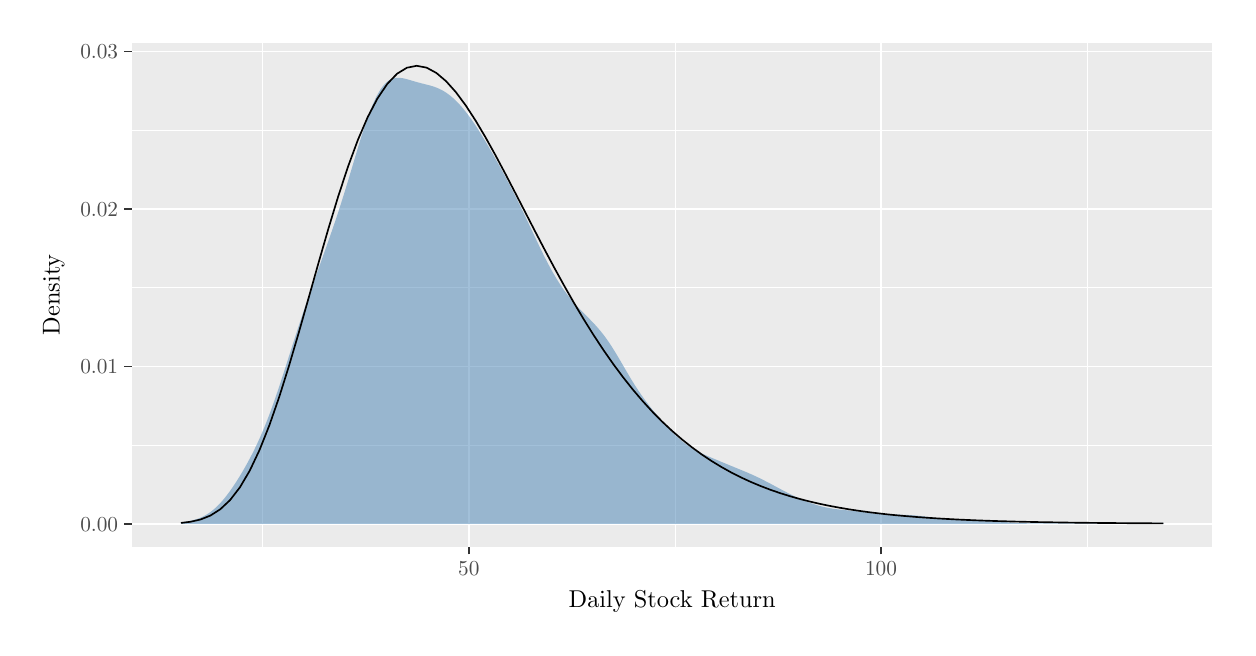
\begin{tikzpicture}[x=1pt,y=1pt]
\definecolor{fillColor}{RGB}{255,255,255}
\path[use as bounding box,fill=fillColor,fill opacity=0.00] (0,0) rectangle (433.62,216.81);
\begin{scope}
\path[clip] (  0.00,  0.00) rectangle (433.62,216.81);
\definecolor{drawColor}{RGB}{255,255,255}
\definecolor{fillColor}{RGB}{255,255,255}

\path[draw=drawColor,line width= 0.6pt,line join=round,line cap=round,fill=fillColor] (  0.00,  0.00) rectangle (433.62,216.81);
\end{scope}
\begin{scope}
\path[clip] ( 37.64, 29.26) rectangle (428.12,211.31);
\definecolor{fillColor}{gray}{0.92}

\path[fill=fillColor] ( 37.64, 29.26) rectangle (428.12,211.31);
\definecolor{drawColor}{RGB}{255,255,255}

\path[draw=drawColor,line width= 0.3pt,line join=round] ( 37.64, 65.97) --
	(428.12, 65.97);

\path[draw=drawColor,line width= 0.3pt,line join=round] ( 37.64,122.84) --
	(428.12,122.84);

\path[draw=drawColor,line width= 0.3pt,line join=round] ( 37.64,179.71) --
	(428.12,179.71);

\path[draw=drawColor,line width= 0.3pt,line join=round] ( 84.90, 29.26) --
	( 84.90,211.31);

\path[draw=drawColor,line width= 0.3pt,line join=round] (233.88, 29.26) --
	(233.88,211.31);

\path[draw=drawColor,line width= 0.3pt,line join=round] (382.87, 29.26) --
	(382.87,211.31);

\path[draw=drawColor,line width= 0.6pt,line join=round] ( 37.64, 37.53) --
	(428.12, 37.53);

\path[draw=drawColor,line width= 0.6pt,line join=round] ( 37.64, 94.40) --
	(428.12, 94.40);

\path[draw=drawColor,line width= 0.6pt,line join=round] ( 37.64,151.28) --
	(428.12,151.28);

\path[draw=drawColor,line width= 0.6pt,line join=round] ( 37.64,208.15) --
	(428.12,208.15);

\path[draw=drawColor,line width= 0.6pt,line join=round] (159.39, 29.26) --
	(159.39,211.31);

\path[draw=drawColor,line width= 0.6pt,line join=round] (308.37, 29.26) --
	(308.37,211.31);
\definecolor{fillColor}{RGB}{70,130,180}

\path[fill=fillColor,fill opacity=0.50] ( 55.39, 38.09) --
	( 56.08, 38.17) --
	( 56.78, 38.26) --
	( 57.47, 38.36) --
	( 58.17, 38.49) --
	( 58.86, 38.63) --
	( 59.56, 38.79) --
	( 60.25, 38.97) --
	( 60.95, 39.18) --
	( 61.64, 39.42) --
	( 62.34, 39.69) --
	( 63.03, 40.00) --
	( 63.73, 40.34) --
	( 64.42, 40.73) --
	( 65.11, 41.16) --
	( 65.81, 41.63) --
	( 66.50, 42.14) --
	( 67.20, 42.70) --
	( 67.89, 43.31) --
	( 68.59, 43.98) --
	( 69.28, 44.68) --
	( 69.98, 45.44) --
	( 70.67, 46.24) --
	( 71.37, 47.08) --
	( 72.06, 47.96) --
	( 72.76, 48.89) --
	( 73.45, 49.86) --
	( 74.15, 50.87) --
	( 74.84, 51.90) --
	( 75.54, 52.98) --
	( 76.23, 54.08) --
	( 76.92, 55.21) --
	( 77.62, 56.38) --
	( 78.31, 57.58) --
	( 79.01, 58.81) --
	( 79.70, 60.08) --
	( 80.40, 61.38) --
	( 81.09, 62.72) --
	( 81.79, 64.11) --
	( 82.48, 65.53) --
	( 83.18, 67.02) --
	( 83.87, 68.55) --
	( 84.57, 70.14) --
	( 85.26, 71.78) --
	( 85.96, 73.48) --
	( 86.65, 75.24) --
	( 87.34, 77.05) --
	( 88.04, 78.93) --
	( 88.73, 80.87) --
	( 89.43, 82.85) --
	( 90.12, 84.88) --
	( 90.82, 86.94) --
	( 91.51, 89.05) --
	( 92.21, 91.18) --
	( 92.90, 93.33) --
	( 93.60, 95.50) --
	( 94.29, 97.68) --
	( 94.99, 99.85) --
	( 95.68,102.03) --
	( 96.38,104.19) --
	( 97.07,106.34) --
	( 97.76,108.47) --
	( 98.46,110.58) --
	( 99.15,112.67) --
	( 99.85,114.73) --
	(100.54,116.78) --
	(101.24,118.80) --
	(101.93,120.81) --
	(102.63,122.80) --
	(103.32,124.77) --
	(104.02,126.72) --
	(104.71,128.67) --
	(105.41,130.62) --
	(106.10,132.55) --
	(106.80,134.49) --
	(107.49,136.44) --
	(108.19,138.39) --
	(108.88,140.36) --
	(109.57,142.35) --
	(110.27,144.36) --
	(110.96,146.40) --
	(111.66,148.47) --
	(112.35,150.57) --
	(113.05,152.72) --
	(113.74,154.91) --
	(114.44,157.13) --
	(115.13,159.39) --
	(115.83,161.68) --
	(116.52,163.99) --
	(117.22,166.32) --
	(117.91,168.65) --
	(118.61,170.98) --
	(119.30,173.29) --
	(119.99,175.57) --
	(120.69,177.81) --
	(121.38,179.98) --
	(122.08,182.08) --
	(122.77,184.09) --
	(123.47,185.98) --
	(124.16,187.77) --
	(124.86,189.42) --
	(125.55,190.95) --
	(126.25,192.35) --
	(126.94,193.60) --
	(127.64,194.70) --
	(128.33,195.64) --
	(129.03,196.45) --
	(129.72,197.11) --
	(130.41,197.65) --
	(131.11,198.07) --
	(131.80,198.38) --
	(132.50,198.59) --
	(133.19,198.69) --
	(133.89,198.71) --
	(134.58,198.67) --
	(135.28,198.58) --
	(135.97,198.45) --
	(136.67,198.28) --
	(137.36,198.09) --
	(138.06,197.89) --
	(138.75,197.69) --
	(139.45,197.48) --
	(140.14,197.28) --
	(140.84,197.09) --
	(141.53,196.90) --
	(142.22,196.72) --
	(142.92,196.55) --
	(143.61,196.37) --
	(144.31,196.20) --
	(145.00,196.02) --
	(145.70,195.82) --
	(146.39,195.61) --
	(147.09,195.38) --
	(147.78,195.12) --
	(148.48,194.83) --
	(149.17,194.50) --
	(149.87,194.14) --
	(150.56,193.73) --
	(151.26,193.29) --
	(151.95,192.81) --
	(152.64,192.28) --
	(153.34,191.70) --
	(154.03,191.08) --
	(154.73,190.42) --
	(155.42,189.72) --
	(156.12,188.98) --
	(156.81,188.20) --
	(157.51,187.38) --
	(158.20,186.51) --
	(158.90,185.61) --
	(159.59,184.68) --
	(160.29,183.71) --
	(160.98,182.71) --
	(161.68,181.68) --
	(162.37,180.63) --
	(163.06,179.55) --
	(163.76,178.44) --
	(164.45,177.31) --
	(165.15,176.16) --
	(165.84,174.99) --
	(166.54,173.81) --
	(167.23,172.61) --
	(167.93,171.40) --
	(168.62,170.18) --
	(169.32,168.94) --
	(170.01,167.69) --
	(170.71,166.43) --
	(171.40,165.16) --
	(172.10,163.87) --
	(172.79,162.57) --
	(173.49,161.26) --
	(174.18,159.93) --
	(174.87,158.59) --
	(175.57,157.23) --
	(176.26,155.86) --
	(176.96,154.47) --
	(177.65,153.06) --
	(178.35,151.64) --
	(179.04,150.20) --
	(179.74,148.75) --
	(180.43,147.28) --
	(181.13,145.81) --
	(181.82,144.33) --
	(182.52,142.85) --
	(183.21,141.37) --
	(183.91,139.89) --
	(184.60,138.43) --
	(185.29,136.99) --
	(185.99,135.56) --
	(186.68,134.16) --
	(187.38,132.79) --
	(188.07,131.45) --
	(188.77,130.15) --
	(189.46,128.89) --
	(190.16,127.68) --
	(190.85,126.50) --
	(191.55,125.36) --
	(192.24,124.27) --
	(192.94,123.22) --
	(193.63,122.21) --
	(194.33,121.25) --
	(195.02,120.32) --
	(195.71,119.43) --
	(196.41,118.57) --
	(197.10,117.74) --
	(197.80,116.95) --
	(198.49,116.18) --
	(199.19,115.43) --
	(199.88,114.71) --
	(200.58,113.99) --
	(201.27,113.29) --
	(201.97,112.59) --
	(202.66,111.90) --
	(203.36,111.19) --
	(204.05,110.48) --
	(204.75,109.74) --
	(205.44,108.99) --
	(206.13,108.20) --
	(206.83,107.38) --
	(207.52,106.53) --
	(208.22,105.64) --
	(208.91,104.70) --
	(209.61,103.72) --
	(210.30,102.70) --
	(211.00,101.64) --
	(211.69,100.54) --
	(212.39, 99.42) --
	(213.08, 98.26) --
	(213.78, 97.09) --
	(214.47, 95.90) --
	(215.17, 94.71) --
	(215.86, 93.51) --
	(216.56, 92.32) --
	(217.25, 91.15) --
	(217.94, 89.99) --
	(218.64, 88.85) --
	(219.33, 87.74) --
	(220.03, 86.66) --
	(220.72, 85.60) --
	(221.42, 84.58) --
	(222.11, 83.58) --
	(222.81, 82.61) --
	(223.50, 81.66) --
	(224.20, 80.75) --
	(224.89, 79.85) --
	(225.59, 78.97) --
	(226.28, 78.11) --
	(226.98, 77.26) --
	(227.67, 76.43) --
	(228.36, 75.61) --
	(229.06, 74.81) --
	(229.75, 74.02) --
	(230.45, 73.25) --
	(231.14, 72.49) --
	(231.84, 71.75) --
	(232.53, 71.03) --
	(233.23, 70.33) --
	(233.92, 69.65) --
	(234.62, 69.00) --
	(235.31, 68.37) --
	(236.01, 67.77) --
	(236.70, 67.20) --
	(237.40, 66.65) --
	(238.09, 66.13) --
	(238.78, 65.65) --
	(239.48, 65.19) --
	(240.17, 64.76) --
	(240.87, 64.35) --
	(241.56, 63.97) --
	(242.26, 63.60) --
	(242.95, 63.25) --
	(243.65, 62.92) --
	(244.34, 62.60) --
	(245.04, 62.29) --
	(245.73, 61.99) --
	(246.43, 61.69) --
	(247.12, 61.40) --
	(247.82, 61.11) --
	(248.51, 60.82) --
	(249.21, 60.53) --
	(249.90, 60.24) --
	(250.59, 59.95) --
	(251.29, 59.66) --
	(251.98, 59.38) --
	(252.68, 59.09) --
	(253.37, 58.80) --
	(254.07, 58.51) --
	(254.76, 58.23) --
	(255.46, 57.94) --
	(256.15, 57.66) --
	(256.85, 57.37) --
	(257.54, 57.09) --
	(258.24, 56.81) --
	(258.93, 56.52) --
	(259.63, 56.23) --
	(260.32, 55.93) --
	(261.01, 55.63) --
	(261.71, 55.32) --
	(262.40, 55.01) --
	(263.10, 54.69) --
	(263.79, 54.36) --
	(264.49, 54.02) --
	(265.18, 53.68) --
	(265.88, 53.33) --
	(266.57, 52.97) --
	(267.27, 52.61) --
	(267.96, 52.25) --
	(268.66, 51.88) --
	(269.35, 51.51) --
	(270.05, 51.13) --
	(270.74, 50.76) --
	(271.43, 50.39) --
	(272.13, 50.02) --
	(272.82, 49.65) --
	(273.52, 49.29) --
	(274.21, 48.93) --
	(274.91, 48.57) --
	(275.60, 48.22) --
	(276.30, 47.88) --
	(276.99, 47.54) --
	(277.69, 47.21) --
	(278.38, 46.89) --
	(279.08, 46.57) --
	(279.77, 46.27) --
	(280.47, 45.98) --
	(281.16, 45.69) --
	(281.86, 45.42) --
	(282.55, 45.16) --
	(283.24, 44.91) --
	(283.94, 44.67) --
	(284.63, 44.45) --
	(285.33, 44.24) --
	(286.02, 44.04) --
	(286.72, 43.86) --
	(287.41, 43.68) --
	(288.11, 43.52) --
	(288.80, 43.38) --
	(289.50, 43.25) --
	(290.19, 43.12) --
	(290.89, 43.01) --
	(291.58, 42.91) --
	(292.28, 42.82) --
	(292.97, 42.73) --
	(293.66, 42.66) --
	(294.36, 42.58) --
	(295.05, 42.51) --
	(295.75, 42.44) --
	(296.44, 42.38) --
	(297.14, 42.31) --
	(297.83, 42.24) --
	(298.53, 42.17) --
	(299.22, 42.09) --
	(299.92, 42.01) --
	(300.61, 41.93) --
	(301.31, 41.85) --
	(302.00, 41.76) --
	(302.70, 41.67) --
	(303.39, 41.58) --
	(304.08, 41.49) --
	(304.78, 41.41) --
	(305.47, 41.32) --
	(306.17, 41.24) --
	(306.86, 41.17) --
	(307.56, 41.10) --
	(308.25, 41.04) --
	(308.95, 40.99) --
	(309.64, 40.95) --
	(310.34, 40.92) --
	(311.03, 40.89) --
	(311.73, 40.87) --
	(312.42, 40.85) --
	(313.12, 40.84) --
	(313.81, 40.83) --
	(314.51, 40.82) --
	(315.20, 40.81) --
	(315.89, 40.80) --
	(316.59, 40.78) --
	(317.28, 40.76) --
	(317.98, 40.73) --
	(318.67, 40.69) --
	(319.37, 40.65) --
	(320.06, 40.60) --
	(320.76, 40.54) --
	(321.45, 40.47) --
	(322.15, 40.40) --
	(322.84, 40.32) --
	(323.54, 40.24) --
	(324.23, 40.15) --
	(324.93, 40.06) --
	(325.62, 39.97) --
	(326.31, 39.88) --
	(327.01, 39.79) --
	(327.70, 39.70) --
	(328.40, 39.61) --
	(329.09, 39.52) --
	(329.79, 39.44) --
	(330.48, 39.37) --
	(331.18, 39.29) --
	(331.87, 39.23) --
	(332.57, 39.16) --
	(333.26, 39.11) --
	(333.96, 39.05) --
	(334.65, 39.01) --
	(335.35, 38.97) --
	(336.04, 38.93) --
	(336.73, 38.90) --
	(337.43, 38.87) --
	(338.12, 38.84) --
	(338.82, 38.82) --
	(339.51, 38.80) --
	(340.21, 38.78) --
	(340.90, 38.76) --
	(341.60, 38.75) --
	(342.29, 38.73) --
	(342.99, 38.71) --
	(343.68, 38.69) --
	(344.38, 38.66) --
	(345.07, 38.64) --
	(345.77, 38.61) --
	(346.46, 38.58) --
	(347.16, 38.54) --
	(347.85, 38.51) --
	(348.54, 38.47) --
	(349.24, 38.42) --
	(349.93, 38.38) --
	(350.63, 38.33) --
	(351.32, 38.28) --
	(352.02, 38.23) --
	(352.71, 38.18) --
	(353.41, 38.13) --
	(354.10, 38.09) --
	(354.80, 38.04) --
	(355.49, 37.99) --
	(356.19, 37.95) --
	(356.88, 37.91) --
	(357.58, 37.87) --
	(358.27, 37.84) --
	(358.96, 37.80) --
	(359.66, 37.78) --
	(360.35, 37.75) --
	(361.05, 37.73) --
	(361.74, 37.72) --
	(362.44, 37.70) --
	(363.13, 37.69) --
	(363.83, 37.69) --
	(364.52, 37.68) --
	(365.22, 37.68) --
	(365.91, 37.68) --
	(366.61, 37.68) --
	(367.30, 37.69) --
	(368.00, 37.69) --
	(368.69, 37.70) --
	(369.38, 37.70) --
	(370.08, 37.71) --
	(370.77, 37.72) --
	(371.47, 37.72) --
	(372.16, 37.73) --
	(372.86, 37.73) --
	(373.55, 37.73) --
	(374.25, 37.73) --
	(374.94, 37.73) --
	(375.64, 37.73) --
	(376.33, 37.73) --
	(377.03, 37.73) --
	(377.72, 37.72) --
	(378.42, 37.72) --
	(379.11, 37.71) --
	(379.81, 37.71) --
	(380.50, 37.71) --
	(381.19, 37.70) --
	(381.89, 37.70) --
	(382.58, 37.70) --
	(383.28, 37.70) --
	(383.97, 37.71) --
	(384.67, 37.71) --
	(385.36, 37.72) --
	(386.06, 37.72) --
	(386.75, 37.73) --
	(387.45, 37.74) --
	(388.14, 37.75) --
	(388.84, 37.76) --
	(389.53, 37.77) --
	(390.23, 37.78) --
	(390.92, 37.79) --
	(391.61, 37.79) --
	(392.31, 37.80) --
	(393.00, 37.81) --
	(393.70, 37.82) --
	(394.39, 37.83) --
	(395.09, 37.84) --
	(395.78, 37.85) --
	(396.48, 37.85) --
	(397.17, 37.86) --
	(397.87, 37.87) --
	(398.56, 37.87) --
	(399.26, 37.88) --
	(399.95, 37.88) --
	(400.65, 37.89) --
	(401.34, 37.89) --
	(402.03, 37.89) --
	(402.73, 37.89) --
	(403.42, 37.89) --
	(404.12, 37.89) --
	(404.81, 37.89) --
	(405.51, 37.89) --
	(406.20, 37.89) --
	(406.90, 37.88) --
	(407.59, 37.88) --
	(408.29, 37.87) --
	(408.98, 37.86) --
	(409.68, 37.85) --
	(410.37, 37.83) --
	(410.37, 37.53) --
	(409.68, 37.53) --
	(408.98, 37.53) --
	(408.29, 37.53) --
	(407.59, 37.53) --
	(406.90, 37.53) --
	(406.20, 37.53) --
	(405.51, 37.53) --
	(404.81, 37.53) --
	(404.12, 37.53) --
	(403.42, 37.53) --
	(402.73, 37.53) --
	(402.03, 37.53) --
	(401.34, 37.53) --
	(400.65, 37.53) --
	(399.95, 37.53) --
	(399.26, 37.53) --
	(398.56, 37.53) --
	(397.87, 37.53) --
	(397.17, 37.53) --
	(396.48, 37.53) --
	(395.78, 37.53) --
	(395.09, 37.53) --
	(394.39, 37.53) --
	(393.70, 37.53) --
	(393.00, 37.53) --
	(392.31, 37.53) --
	(391.61, 37.53) --
	(390.92, 37.53) --
	(390.23, 37.53) --
	(389.53, 37.53) --
	(388.84, 37.53) --
	(388.14, 37.53) --
	(387.45, 37.53) --
	(386.75, 37.53) --
	(386.06, 37.53) --
	(385.36, 37.53) --
	(384.67, 37.53) --
	(383.97, 37.53) --
	(383.28, 37.53) --
	(382.58, 37.53) --
	(381.89, 37.53) --
	(381.19, 37.53) --
	(380.50, 37.53) --
	(379.81, 37.53) --
	(379.11, 37.53) --
	(378.42, 37.53) --
	(377.72, 37.53) --
	(377.03, 37.53) --
	(376.33, 37.53) --
	(375.64, 37.53) --
	(374.94, 37.53) --
	(374.25, 37.53) --
	(373.55, 37.53) --
	(372.86, 37.53) --
	(372.16, 37.53) --
	(371.47, 37.53) --
	(370.77, 37.53) --
	(370.08, 37.53) --
	(369.38, 37.53) --
	(368.69, 37.53) --
	(368.00, 37.53) --
	(367.30, 37.53) --
	(366.61, 37.53) --
	(365.91, 37.53) --
	(365.22, 37.53) --
	(364.52, 37.53) --
	(363.83, 37.53) --
	(363.13, 37.53) --
	(362.44, 37.53) --
	(361.74, 37.53) --
	(361.05, 37.53) --
	(360.35, 37.53) --
	(359.66, 37.53) --
	(358.96, 37.53) --
	(358.27, 37.53) --
	(357.58, 37.53) --
	(356.88, 37.53) --
	(356.19, 37.53) --
	(355.49, 37.53) --
	(354.80, 37.53) --
	(354.10, 37.53) --
	(353.41, 37.53) --
	(352.71, 37.53) --
	(352.02, 37.53) --
	(351.32, 37.53) --
	(350.63, 37.53) --
	(349.93, 37.53) --
	(349.24, 37.53) --
	(348.54, 37.53) --
	(347.85, 37.53) --
	(347.16, 37.53) --
	(346.46, 37.53) --
	(345.77, 37.53) --
	(345.07, 37.53) --
	(344.38, 37.53) --
	(343.68, 37.53) --
	(342.99, 37.53) --
	(342.29, 37.53) --
	(341.60, 37.53) --
	(340.90, 37.53) --
	(340.21, 37.53) --
	(339.51, 37.53) --
	(338.82, 37.53) --
	(338.12, 37.53) --
	(337.43, 37.53) --
	(336.73, 37.53) --
	(336.04, 37.53) --
	(335.35, 37.53) --
	(334.65, 37.53) --
	(333.96, 37.53) --
	(333.26, 37.53) --
	(332.57, 37.53) --
	(331.87, 37.53) --
	(331.18, 37.53) --
	(330.48, 37.53) --
	(329.79, 37.53) --
	(329.09, 37.53) --
	(328.40, 37.53) --
	(327.70, 37.53) --
	(327.01, 37.53) --
	(326.31, 37.53) --
	(325.62, 37.53) --
	(324.93, 37.53) --
	(324.23, 37.53) --
	(323.54, 37.53) --
	(322.84, 37.53) --
	(322.15, 37.53) --
	(321.45, 37.53) --
	(320.76, 37.53) --
	(320.06, 37.53) --
	(319.37, 37.53) --
	(318.67, 37.53) --
	(317.98, 37.53) --
	(317.28, 37.53) --
	(316.59, 37.53) --
	(315.89, 37.53) --
	(315.20, 37.53) --
	(314.51, 37.53) --
	(313.81, 37.53) --
	(313.12, 37.53) --
	(312.42, 37.53) --
	(311.73, 37.53) --
	(311.03, 37.53) --
	(310.34, 37.53) --
	(309.64, 37.53) --
	(308.95, 37.53) --
	(308.25, 37.53) --
	(307.56, 37.53) --
	(306.86, 37.53) --
	(306.17, 37.53) --
	(305.47, 37.53) --
	(304.78, 37.53) --
	(304.08, 37.53) --
	(303.39, 37.53) --
	(302.70, 37.53) --
	(302.00, 37.53) --
	(301.31, 37.53) --
	(300.61, 37.53) --
	(299.92, 37.53) --
	(299.22, 37.53) --
	(298.53, 37.53) --
	(297.83, 37.53) --
	(297.14, 37.53) --
	(296.44, 37.53) --
	(295.75, 37.53) --
	(295.05, 37.53) --
	(294.36, 37.53) --
	(293.66, 37.53) --
	(292.97, 37.53) --
	(292.28, 37.53) --
	(291.58, 37.53) --
	(290.89, 37.53) --
	(290.19, 37.53) --
	(289.50, 37.53) --
	(288.80, 37.53) --
	(288.11, 37.53) --
	(287.41, 37.53) --
	(286.72, 37.53) --
	(286.02, 37.53) --
	(285.33, 37.53) --
	(284.63, 37.53) --
	(283.94, 37.53) --
	(283.24, 37.53) --
	(282.55, 37.53) --
	(281.86, 37.53) --
	(281.16, 37.53) --
	(280.47, 37.53) --
	(279.77, 37.53) --
	(279.08, 37.53) --
	(278.38, 37.53) --
	(277.69, 37.53) --
	(276.99, 37.53) --
	(276.30, 37.53) --
	(275.60, 37.53) --
	(274.91, 37.53) --
	(274.21, 37.53) --
	(273.52, 37.53) --
	(272.82, 37.53) --
	(272.13, 37.53) --
	(271.43, 37.53) --
	(270.74, 37.53) --
	(270.05, 37.53) --
	(269.35, 37.53) --
	(268.66, 37.53) --
	(267.96, 37.53) --
	(267.27, 37.53) --
	(266.57, 37.53) --
	(265.88, 37.53) --
	(265.18, 37.53) --
	(264.49, 37.53) --
	(263.79, 37.53) --
	(263.10, 37.53) --
	(262.40, 37.53) --
	(261.71, 37.53) --
	(261.01, 37.53) --
	(260.32, 37.53) --
	(259.63, 37.53) --
	(258.93, 37.53) --
	(258.24, 37.53) --
	(257.54, 37.53) --
	(256.85, 37.53) --
	(256.15, 37.53) --
	(255.46, 37.53) --
	(254.76, 37.53) --
	(254.07, 37.53) --
	(253.37, 37.53) --
	(252.68, 37.53) --
	(251.98, 37.53) --
	(251.29, 37.53) --
	(250.59, 37.53) --
	(249.90, 37.53) --
	(249.21, 37.53) --
	(248.51, 37.53) --
	(247.82, 37.53) --
	(247.12, 37.53) --
	(246.43, 37.53) --
	(245.73, 37.53) --
	(245.04, 37.53) --
	(244.34, 37.53) --
	(243.65, 37.53) --
	(242.95, 37.53) --
	(242.26, 37.53) --
	(241.56, 37.53) --
	(240.87, 37.53) --
	(240.17, 37.53) --
	(239.48, 37.53) --
	(238.78, 37.53) --
	(238.09, 37.53) --
	(237.40, 37.53) --
	(236.70, 37.53) --
	(236.01, 37.53) --
	(235.31, 37.53) --
	(234.62, 37.53) --
	(233.92, 37.53) --
	(233.23, 37.53) --
	(232.53, 37.53) --
	(231.84, 37.53) --
	(231.14, 37.53) --
	(230.45, 37.53) --
	(229.75, 37.53) --
	(229.06, 37.53) --
	(228.36, 37.53) --
	(227.67, 37.53) --
	(226.98, 37.53) --
	(226.28, 37.53) --
	(225.59, 37.53) --
	(224.89, 37.53) --
	(224.20, 37.53) --
	(223.50, 37.53) --
	(222.81, 37.53) --
	(222.11, 37.53) --
	(221.42, 37.53) --
	(220.72, 37.53) --
	(220.03, 37.53) --
	(219.33, 37.53) --
	(218.64, 37.53) --
	(217.94, 37.53) --
	(217.25, 37.53) --
	(216.56, 37.53) --
	(215.86, 37.53) --
	(215.17, 37.53) --
	(214.47, 37.53) --
	(213.78, 37.53) --
	(213.08, 37.53) --
	(212.39, 37.53) --
	(211.69, 37.53) --
	(211.00, 37.53) --
	(210.30, 37.53) --
	(209.61, 37.53) --
	(208.91, 37.53) --
	(208.22, 37.53) --
	(207.52, 37.53) --
	(206.83, 37.53) --
	(206.13, 37.53) --
	(205.44, 37.53) --
	(204.75, 37.53) --
	(204.05, 37.53) --
	(203.36, 37.53) --
	(202.66, 37.53) --
	(201.97, 37.53) --
	(201.27, 37.53) --
	(200.58, 37.53) --
	(199.88, 37.53) --
	(199.19, 37.53) --
	(198.49, 37.53) --
	(197.80, 37.53) --
	(197.10, 37.53) --
	(196.41, 37.53) --
	(195.71, 37.53) --
	(195.02, 37.53) --
	(194.33, 37.53) --
	(193.63, 37.53) --
	(192.94, 37.53) --
	(192.24, 37.53) --
	(191.55, 37.53) --
	(190.85, 37.53) --
	(190.16, 37.53) --
	(189.46, 37.53) --
	(188.77, 37.53) --
	(188.07, 37.53) --
	(187.38, 37.53) --
	(186.68, 37.53) --
	(185.99, 37.53) --
	(185.29, 37.53) --
	(184.60, 37.53) --
	(183.91, 37.53) --
	(183.21, 37.53) --
	(182.52, 37.53) --
	(181.82, 37.53) --
	(181.13, 37.53) --
	(180.43, 37.53) --
	(179.74, 37.53) --
	(179.04, 37.53) --
	(178.35, 37.53) --
	(177.65, 37.53) --
	(176.96, 37.53) --
	(176.26, 37.53) --
	(175.57, 37.53) --
	(174.87, 37.53) --
	(174.18, 37.53) --
	(173.49, 37.53) --
	(172.79, 37.53) --
	(172.10, 37.53) --
	(171.40, 37.53) --
	(170.71, 37.53) --
	(170.01, 37.53) --
	(169.32, 37.53) --
	(168.62, 37.53) --
	(167.93, 37.53) --
	(167.23, 37.53) --
	(166.54, 37.53) --
	(165.84, 37.53) --
	(165.15, 37.53) --
	(164.45, 37.53) --
	(163.76, 37.53) --
	(163.06, 37.53) --
	(162.37, 37.53) --
	(161.68, 37.53) --
	(160.98, 37.53) --
	(160.29, 37.53) --
	(159.59, 37.53) --
	(158.90, 37.53) --
	(158.20, 37.53) --
	(157.51, 37.53) --
	(156.81, 37.53) --
	(156.12, 37.53) --
	(155.42, 37.53) --
	(154.73, 37.53) --
	(154.03, 37.53) --
	(153.34, 37.53) --
	(152.64, 37.53) --
	(151.95, 37.53) --
	(151.26, 37.53) --
	(150.56, 37.53) --
	(149.87, 37.53) --
	(149.17, 37.53) --
	(148.48, 37.53) --
	(147.78, 37.53) --
	(147.09, 37.53) --
	(146.39, 37.53) --
	(145.70, 37.53) --
	(145.00, 37.53) --
	(144.31, 37.53) --
	(143.61, 37.53) --
	(142.92, 37.53) --
	(142.22, 37.53) --
	(141.53, 37.53) --
	(140.84, 37.53) --
	(140.14, 37.53) --
	(139.45, 37.53) --
	(138.75, 37.53) --
	(138.06, 37.53) --
	(137.36, 37.53) --
	(136.67, 37.53) --
	(135.97, 37.53) --
	(135.28, 37.53) --
	(134.58, 37.53) --
	(133.89, 37.53) --
	(133.19, 37.53) --
	(132.50, 37.53) --
	(131.80, 37.53) --
	(131.11, 37.53) --
	(130.41, 37.53) --
	(129.72, 37.53) --
	(129.03, 37.53) --
	(128.33, 37.53) --
	(127.64, 37.53) --
	(126.94, 37.53) --
	(126.25, 37.53) --
	(125.55, 37.53) --
	(124.86, 37.53) --
	(124.16, 37.53) --
	(123.47, 37.53) --
	(122.77, 37.53) --
	(122.08, 37.53) --
	(121.38, 37.53) --
	(120.69, 37.53) --
	(119.99, 37.53) --
	(119.30, 37.53) --
	(118.61, 37.53) --
	(117.91, 37.53) --
	(117.22, 37.53) --
	(116.52, 37.53) --
	(115.83, 37.53) --
	(115.13, 37.53) --
	(114.44, 37.53) --
	(113.74, 37.53) --
	(113.05, 37.53) --
	(112.35, 37.53) --
	(111.66, 37.53) --
	(110.96, 37.53) --
	(110.27, 37.53) --
	(109.57, 37.53) --
	(108.88, 37.53) --
	(108.19, 37.53) --
	(107.49, 37.53) --
	(106.80, 37.53) --
	(106.10, 37.53) --
	(105.41, 37.53) --
	(104.71, 37.53) --
	(104.02, 37.53) --
	(103.32, 37.53) --
	(102.63, 37.53) --
	(101.93, 37.53) --
	(101.24, 37.53) --
	(100.54, 37.53) --
	( 99.85, 37.53) --
	( 99.15, 37.53) --
	( 98.46, 37.53) --
	( 97.76, 37.53) --
	( 97.07, 37.53) --
	( 96.38, 37.53) --
	( 95.68, 37.53) --
	( 94.99, 37.53) --
	( 94.29, 37.53) --
	( 93.60, 37.53) --
	( 92.90, 37.53) --
	( 92.21, 37.53) --
	( 91.51, 37.53) --
	( 90.82, 37.53) --
	( 90.12, 37.53) --
	( 89.43, 37.53) --
	( 88.73, 37.53) --
	( 88.04, 37.53) --
	( 87.34, 37.53) --
	( 86.65, 37.53) --
	( 85.96, 37.53) --
	( 85.26, 37.53) --
	( 84.57, 37.53) --
	( 83.87, 37.53) --
	( 83.18, 37.53) --
	( 82.48, 37.53) --
	( 81.79, 37.53) --
	( 81.09, 37.53) --
	( 80.40, 37.53) --
	( 79.70, 37.53) --
	( 79.01, 37.53) --
	( 78.31, 37.53) --
	( 77.62, 37.53) --
	( 76.92, 37.53) --
	( 76.23, 37.53) --
	( 75.54, 37.53) --
	( 74.84, 37.53) --
	( 74.15, 37.53) --
	( 73.45, 37.53) --
	( 72.76, 37.53) --
	( 72.06, 37.53) --
	( 71.37, 37.53) --
	( 70.67, 37.53) --
	( 69.98, 37.53) --
	( 69.28, 37.53) --
	( 68.59, 37.53) --
	( 67.89, 37.53) --
	( 67.20, 37.53) --
	( 66.50, 37.53) --
	( 65.81, 37.53) --
	( 65.11, 37.53) --
	( 64.42, 37.53) --
	( 63.73, 37.53) --
	( 63.03, 37.53) --
	( 62.34, 37.53) --
	( 61.64, 37.53) --
	( 60.95, 37.53) --
	( 60.25, 37.53) --
	( 59.56, 37.53) --
	( 58.86, 37.53) --
	( 58.17, 37.53) --
	( 57.47, 37.53) --
	( 56.78, 37.53) --
	( 56.08, 37.53) --
	( 55.39, 37.53) --
	cycle;
\definecolor{drawColor}{RGB}{0,0,0}

\path[draw=drawColor,line width= 0.6pt,line join=round] ( 55.39, 37.85) --
	( 58.94, 38.28) --
	( 62.49, 39.10) --
	( 66.04, 40.52) --
	( 69.59, 42.78) --
	( 73.14, 46.11) --
	( 76.69, 50.71) --
	( 80.24, 56.73) --
	( 83.79, 64.22) --
	( 87.34, 73.14) --
	( 90.89, 83.36) --
	( 94.44, 94.65) --
	( 97.99,106.71) --
	(101.54,119.22) --
	(105.09,131.80) --
	(108.64,144.10) --
	(112.19,155.78) --
	(115.74,166.55) --
	(119.29,176.17) --
	(122.84,184.43) --
	(126.39,191.23) --
	(129.94,196.48) --
	(133.49,200.18) --
	(137.04,202.34) --
	(140.58,203.03) --
	(144.13,202.37) --
	(147.68,200.45) --
	(151.23,197.43) --
	(154.78,193.45) --
	(158.33,188.66) --
	(161.88,183.19) --
	(165.43,177.20) --
	(168.98,170.82) --
	(172.53,164.15) --
	(176.08,157.32) --
	(179.63,150.43) --
	(183.18,143.54) --
	(186.73,136.74) --
	(190.28,130.09) --
	(193.83,123.63) --
	(197.38,117.40) --
	(200.93,111.43) --
	(204.48,105.75) --
	(208.03,100.36) --
	(211.58, 95.28) --
	(215.13, 90.51) --
	(218.68, 86.04) --
	(222.23, 81.87) --
	(225.78, 77.99) --
	(229.33, 74.40) --
	(232.88, 71.08) --
	(236.43, 68.02) --
	(239.98, 65.21) --
	(243.53, 62.62) --
	(247.08, 60.25) --
	(250.63, 58.09) --
	(254.18, 56.11) --
	(257.73, 54.31) --
	(261.28, 52.67) --
	(264.83, 51.19) --
	(268.38, 49.83) --
	(271.93, 48.61) --
	(275.48, 47.50) --
	(279.03, 46.50) --
	(282.58, 45.59) --
	(286.13, 44.77) --
	(289.68, 44.03) --
	(293.23, 43.37) --
	(296.78, 42.77) --
	(300.33, 42.23) --
	(303.88, 41.74) --
	(307.43, 41.31) --
	(310.98, 40.91) --
	(314.53, 40.56) --
	(318.08, 40.25) --
	(321.63, 39.96) --
	(325.18, 39.71) --
	(328.73, 39.48) --
	(332.27, 39.28) --
	(335.82, 39.09) --
	(339.37, 38.93) --
	(342.92, 38.78) --
	(346.47, 38.65) --
	(350.02, 38.53) --
	(353.57, 38.43) --
	(357.12, 38.33) --
	(360.67, 38.25) --
	(364.22, 38.17) --
	(367.77, 38.11) --
	(371.32, 38.05) --
	(374.87, 37.99) --
	(378.42, 37.94) --
	(381.97, 37.90) --
	(385.52, 37.86) --
	(389.07, 37.83) --
	(392.62, 37.80) --
	(396.17, 37.77) --
	(399.72, 37.74) --
	(403.27, 37.72) --
	(406.82, 37.70) --
	(410.37, 37.68);
\end{scope}
\begin{scope}
\path[clip] (  0.00,  0.00) rectangle (433.62,216.81);
\definecolor{drawColor}{gray}{0.30}

\node[text=drawColor,anchor=base east,inner sep=0pt, outer sep=0pt, scale=  0.77] at ( 32.69, 34.88) {0.00};

\node[text=drawColor,anchor=base east,inner sep=0pt, outer sep=0pt, scale=  0.77] at ( 32.69, 91.75) {0.01};

\node[text=drawColor,anchor=base east,inner sep=0pt, outer sep=0pt, scale=  0.77] at ( 32.69,148.63) {0.02};

\node[text=drawColor,anchor=base east,inner sep=0pt, outer sep=0pt, scale=  0.77] at ( 32.69,205.50) {0.03};
\end{scope}
\begin{scope}
\path[clip] (  0.00,  0.00) rectangle (433.62,216.81);
\definecolor{drawColor}{gray}{0.20}

\path[draw=drawColor,line width= 0.6pt,line join=round] ( 34.89, 37.53) --
	( 37.64, 37.53);

\path[draw=drawColor,line width= 0.6pt,line join=round] ( 34.89, 94.40) --
	( 37.64, 94.40);

\path[draw=drawColor,line width= 0.6pt,line join=round] ( 34.89,151.28) --
	( 37.64,151.28);

\path[draw=drawColor,line width= 0.6pt,line join=round] ( 34.89,208.15) --
	( 37.64,208.15);
\end{scope}
\begin{scope}
\path[clip] (  0.00,  0.00) rectangle (433.62,216.81);
\definecolor{drawColor}{gray}{0.20}

\path[draw=drawColor,line width= 0.6pt,line join=round] (159.39, 26.51) --
	(159.39, 29.26);

\path[draw=drawColor,line width= 0.6pt,line join=round] (308.37, 26.51) --
	(308.37, 29.26);
\end{scope}
\begin{scope}
\path[clip] (  0.00,  0.00) rectangle (433.62,216.81);
\definecolor{drawColor}{gray}{0.30}

\node[text=drawColor,anchor=base,inner sep=0pt, outer sep=0pt, scale=  0.77] at (159.39, 19.00) {50};

\node[text=drawColor,anchor=base,inner sep=0pt, outer sep=0pt, scale=  0.77] at (308.37, 19.00) {100};
\end{scope}
\begin{scope}
\path[clip] (  0.00,  0.00) rectangle (433.62,216.81);
\definecolor{drawColor}{RGB}{0,0,0}

\node[text=drawColor,anchor=base,inner sep=0pt, outer sep=0pt, scale=  0.88] at (232.88,  7.44) {Daily Stock Return};
\end{scope}
\begin{scope}
\path[clip] (  0.00,  0.00) rectangle (433.62,216.81);
\definecolor{drawColor}{RGB}{0,0,0}

\node[text=drawColor,rotate= 90.00,anchor=base,inner sep=0pt, outer sep=0pt, scale=  0.88] at ( 11.56,120.28) {Density};
\end{scope}
\end{tikzpicture}

\caption{Daily Basis Stock Return Density}
\label{p:logdensity}
\floatfoot{
The above density function has been constructed over three distinctive groups of 10000 samples eachs. All samples have been constructed following \cref{eq:Scontinuous}. The arguments are set with the following value, $\alpha = 0$, $\sigma = 30\%$. The black density belongs to the log--normal curve with mean and standard deviation such as described in [REF]. The time frame is one year ($t = 1$) and period between each measure, namely $dt$ has been set to $500^{-1}$. 
}
\end{figure}

%%%%%%%%%%%%%%%%%%%%%%%%%%%%%%%%%%%%%%%%%%%%%%%%
% SUBSECTION: Flaws
%%%%%%%%%%%%%%%%%%%%%%%%%%%%%%%%%%%%%%%%%%%%%%%%
\section{Flaws}
\label{sec:Flaws}

Even if the \cref{eq:Scontinuous} is used to model the stock price process, it exists some lacks with the observed real processes. The analysis ([CHA REF]) mainly covers the following discrepancy of the model against empirical results.
  
The volatility appearing in the aformentioned underlying model (\ref{eq:Scontinuous}) is constant as time passes.
Even if this consideration can be considered as true for short period of time, it is not the case over the long--run \citet{teneng2011limitations}.
Other model substitutes the process defined throughout this chapter with other ones including stochastic volatility processes, making it changing over time.
For this purpose, the Heston's model is developed in this current master thesis, which encompasses two stochastic processes, a geometric Brownian motion [???? + REF] for the stock price diffusion model [DIFUSION??] and a mean-reverting CIR model to compute the volatility as a stochastic process.
This model is exposed in \cref{sec:Heston}.

Following [REF and REF], the uderlying log--returns distribution is characterized by the normal law. Consequently, the random variable $\St$, at the fixed time $t$, is normal. 
However, according to empirical results, the random variable $d\St$ do not fit with the normal bell curve (\citet{clark1973}).
Therefore if the price changes are not normally distribution neither is the log--return and thus $\St$, at a fixed time $t$, is not log--normally distributed.
Along with the Heston model, another one is considerd; the Merton's jump--diffusion model. Both are able to modify the skewness and kurtosis of the log--return distibution curve. The Merton framework is developed in \cref{sec:MixedJump}. 
%%%%%%%%%%%%%%%%%%%%%%%%%%%%%%%%%%%%%%%%%%%%%%%%%%%%%%%%%%%%%%%%%%%%%%%%%%%%%%%%
%
%  CHAPTER:The \BSM model
%
%%%%%%%%%%%%%%%%%%%%%%%%%%%%%%%%%%%%%%%%%%%%%%%%%%%%%%%%%%%%%%%%%%%%%%%%%%%%%%%%
\chapter{The \BSM model}
\label{cha:bsm}


%%%%%%%%%%%%%%%%%%%%%%%%%%%%%%%%%%%%%%%%%%%%%%%%
% SECTION: OverView
%%%%%%%%%%%%%%%%%%%%%%%%%%%%%%%%%%%%%%%%%%%%%%%%
\section{Overview}
\label{sec:bsm:overview}

In this present section the Black--Scholes--Merton model is explained and developed. Stricly speaking, it would be talked about the BSM (Black--Scholes--Merton) model but not BSM equation. In turn the equation would be refered to as the BS (Black and Scholes) equation. This distinction is made because the model encompasses the derivation of the BS equation, either using the CAPM (Capital Asset Pricing Model) for \citet{bs} or  by setting up a riskless portfolio providing an expected return identiacal to risk-free rate for \citet{merton73}.

The BSM model is meant to provide the non arbitrage price of derivative assets such as european stock option (\citet{hull}). In the present master thesis the model derived from the BS formula is focused on the pricing of one of a kind trivial derivative, the vanilla call option.

In order to price call option throughout the model highlighted in this present chapter, some contraints have been set by \citet{bs}. 
The section \ref{sec:Assumptions} quotes the assumptions made to keep the model usage between boundaries. In latter chapter however it will be shown how the model is relevant by going on the edge and even beyond these constraints.


%%%%%%%%%%%%%%%%%%%%%%%%%%%%%%%%%%%%%%%%%%%%%%%%
% SECTION: Assumptions
%%%%%%%%%%%%%%%%%%%%%%%%%%%%%%%%%%%%%%%%%%%%%%%%
\section{Assumptions}
\label{sec:bsm:assumptions}

\citet{bs} have provided a framework defining a bunch of constraints qualified as "ideal conditions" under which the market would behave in order to make the BS equation works with accuracy. All of these conditions are below--mentioned.

\begin{enumerate}
  \item The short-term risk free rate $r$ is known and constant
  \item The stock return involving in the computation of BS equation is lognormally distributed with constant mean and variance rate
  \item No dividend are provided with the considered share of stock
  \item The option considered within the computation is european
  \item The price for bid and ask quote are identical. It means that there is no bid--ask spread to be considerered
  \item Share of stock can be divided into any portions such as needed for the computation
  \item Short selling is allowed with no penalties
\end{enumerate}


%%%%%%%%%%%%%%%%%%%%%%%%%%%%%%%%%%%%%%%%%%%%%%%%
% SECTION: The partial differential BSM equation
%%%%%%%%%%%%%%%%%%%%%%%%%%%%%%%%%%%%%%%%%%%%%%%%
\section{The \BSM equation}
\label{sec:bsm:equation}

The pricing method of an option underpinned by the BSM model is closely related to an underlying for which its price $\St$ is random and log--normally distributed, such the one developed in chapter \ref{cha:underlying} throughout equation \ref{eq:Scontinuous} (\citet{bs}).

In order to provide a unique fair price to a stock option (e.g. a vanilla european call option) which depends on an underlying such as described above, all the uncertainty associated to the stock price motion has to disappear. To do so, one have to first construct such a portofolio $X(t)$ which encompasses the same source on uncertainty as the option itself, i.e., the geometric brownian motion $\St$ and then choosing the adequate position $\Delta(t)$ to take  so that all randomness cancels out (\citet{shreve}).
 
\begin{align}
  \dportfolio \label{eq:dportfolio} \\ 
  \intertext{The goal is to hedge dynamically the position taken in the option. It means that the position has to be frequently rebalanced. Consequently, at any times, the present value of the changes occuring in the portfolio, due to stock price evolution should be equal to the one occuring in the derivative. The only way to achieve this equality is to adapt the delta (\citet{shreve}).}
   d\left(e^{-rt} X\left(t\right)\right) &= d\left(e^{-rt} \ct \right)
\intertext{In that way, one can take a position in the derivatives (short / long) and hedge them by taking $\pm \Delta(t)$ shares of stock. $X(0)$ being the price of the call at time zero}
 X\left(0\right) &= c\left(0, S\left(0\right)\right)
\end{align}




Following the method forementioned, the BSM differential equation is given by equation (\ref{eq:bsm:bsm:eq}),  with terminal condition (\ref{eq:BSMterminal}) and boundary condition (\ref{eq:BSMboundary0}) -- (\ref{eq:BSMboundaryinf}), (\citet{shreve}).

\begin{center}
  \begin{equation}
     \BSMeq{x}
    \label{eq:bsm:bsm:eq}
  \end{equation}
\end{center}
 
\begin{center}
  \begin{equation}
    \call{T}{x} = \left(x - K\right) ^+
    \label{eq:BSMterminal}
  \end{equation}
\end{center}

Whilst the terminal condition focuses on the value taken at maturity, the boundary conditions fix some constraints on the extreme values likely to be taken by the shares of stock at any times during the option life. 
In that regard, the boundary condition (\ref{eq:BSMboundary0}) shows that an option with an worthless underlying is itself valueless, while whenever the option is deep in the money, simulated with $x = \infty$ (\ref{eq:BSMboundaryinf}), the value of the derivative is equal to the value of a forward contract involving the same underlying and with the same maturity date.

\begin{center}
  \begin{equation}
    \call{t}{0} = 0
    \label{eq:BSMboundary0}
  \end{equation}
\end{center}

\begin{center}
  \begin{equation}
    \lim_{x\to\infty} \left[ \call{t}{x} - \left(x - e^{-r \left(T - t \right)} \right) \right] = 0
    \label{eq:BSMboundaryinf}
  \end{equation}
\end{center}
 
%%%%%%%%%%%%%%%%%%%%%%%%%%%%%%%%%%%%%%%%%%%%%%%%
% SECTION: Solution for vanilla option pricing method
%%%%%%%%%%%%%%%%%%%%%%%%%%%%%%%%%%%%%%%%%%%%%%%%
\section{Solution for vanilla option pricing method}
\label{sec:Solution for vanilla option pricing method}


According to the terminal (\ref{eq:BSMterminal}) and boundaries conditions (\ref{eq:BSMboundary0}, \ref{eq:BSMboundaryinf}), the Black--Scholes--Merton solution for call option happens to be given by equation (\ref{eq:bsm:bsm:sol}), (\citet{shreve}). 
The right hand side of the equation, $\ct$, denotes the price of a call option depending on the time to maturity and the stock price at that time.
In addition to these arguments, two other parameters are required, the strike ($k$) and the riskless interest rate ($r$).

\begin{align}
    \BSMsol
    \label{eq:bsm:bsm:sol}
\intertext{with}
    \dpm
    \label{eq:dpm}
\end{align}








% \begin{figure}[!h]
% \centering
% % Created by tikzDevice version 0.11 on 2018-04-08 08:39:42
% !TEX encoding = UTF-8 Unicode
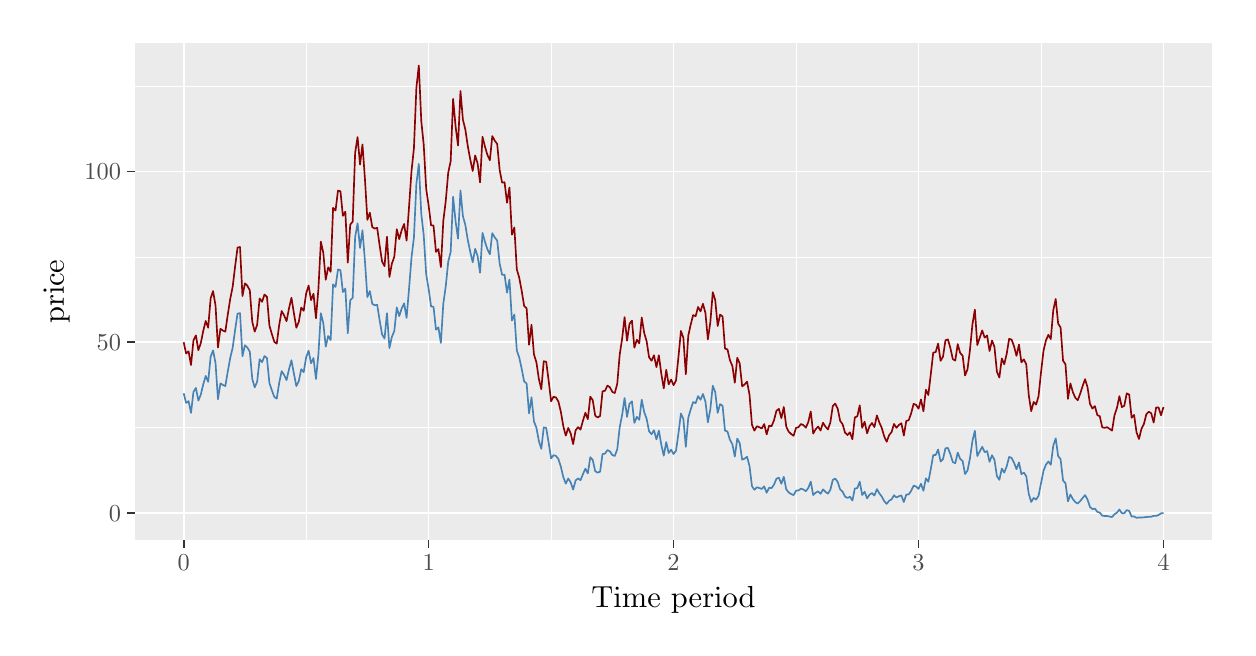
\begin{tikzpicture}[x=1pt,y=1pt]
\definecolor{fillColor}{RGB}{255,255,255}
\path[use as bounding box,fill=fillColor,fill opacity=0.00] (0,0) rectangle (433.62,216.81);
\begin{scope}
\path[clip] (  0.00,  0.00) rectangle (433.62,216.81);
\definecolor{drawColor}{RGB}{255,255,255}
\definecolor{fillColor}{RGB}{255,255,255}

\path[draw=drawColor,line width= 0.6pt,line join=round,line cap=round,fill=fillColor] (  0.00,  0.00) rectangle (433.62,216.81);
\end{scope}
\begin{scope}
\path[clip] ( 38.67, 31.53) rectangle (428.12,211.31);
\definecolor{fillColor}{gray}{0.92}

\path[fill=fillColor] ( 38.67, 31.53) rectangle (428.12,211.31);
\definecolor{drawColor}{RGB}{255,255,255}

\path[draw=drawColor,line width= 0.3pt,line join=round] ( 38.67, 72.27) --
	(428.12, 72.27);

\path[draw=drawColor,line width= 0.3pt,line join=round] ( 38.67,133.96) --
	(428.12,133.96);

\path[draw=drawColor,line width= 0.3pt,line join=round] ( 38.67,195.66) --
	(428.12,195.66);

\path[draw=drawColor,line width= 0.3pt,line join=round] (100.63, 31.53) --
	(100.63,211.31);

\path[draw=drawColor,line width= 0.3pt,line join=round] (189.14, 31.53) --
	(189.14,211.31);

\path[draw=drawColor,line width= 0.3pt,line join=round] (277.65, 31.53) --
	(277.65,211.31);

\path[draw=drawColor,line width= 0.3pt,line join=round] (366.16, 31.53) --
	(366.16,211.31);

\path[draw=drawColor,line width= 0.6pt,line join=round] ( 38.67, 41.43) --
	(428.12, 41.43);

\path[draw=drawColor,line width= 0.6pt,line join=round] ( 38.67,103.12) --
	(428.12,103.12);

\path[draw=drawColor,line width= 0.6pt,line join=round] ( 38.67,164.81) --
	(428.12,164.81);

\path[draw=drawColor,line width= 0.6pt,line join=round] ( 56.37, 31.53) --
	( 56.37,211.31);

\path[draw=drawColor,line width= 0.6pt,line join=round] (144.88, 31.53) --
	(144.88,211.31);

\path[draw=drawColor,line width= 0.6pt,line join=round] (233.39, 31.53) --
	(233.39,211.31);

\path[draw=drawColor,line width= 0.6pt,line join=round] (321.91, 31.53) --
	(321.91,211.31);

\path[draw=drawColor,line width= 0.6pt,line join=round] (410.42, 31.53) --
	(410.42,211.31);
\definecolor{drawColor}{RGB}{70,130,180}

\path[draw=drawColor,line width= 0.6pt,line join=round] ( 56.37, 84.70) --
	( 57.25, 81.22) --
	( 58.14, 81.84) --
	( 59.02, 77.61) --
	( 59.91, 85.17) --
	( 60.79, 86.64) --
	( 61.68, 82.04) --
	( 62.57, 84.24) --
	( 63.45, 87.95) --
	( 64.34, 90.96) --
	( 65.22, 88.84) --
	( 66.11, 97.91) --
	( 66.99,100.19) --
	( 67.88, 95.63) --
	( 68.76, 82.55) --
	( 69.65, 88.29) --
	( 70.53, 87.71) --
	( 71.42, 87.30) --
	( 72.30, 92.52) --
	( 73.19, 97.44) --
	( 74.07,101.15) --
	( 74.96,107.58) --
	( 75.84,113.49) --
	( 76.73,113.64) --
	( 77.61, 98.09) --
	( 78.50,102.04) --
	( 79.38,101.23) --
	( 80.27, 99.73) --
	( 81.15, 89.90) --
	( 82.04, 86.83) --
	( 82.92, 88.88) --
	( 83.81, 97.00) --
	( 84.69, 95.94) --
	( 85.58, 98.16) --
	( 86.46, 97.41) --
	( 87.35, 88.45) --
	( 88.23, 85.79) --
	( 89.12, 83.37) --
	( 90.00, 82.76) --
	( 90.89, 88.45) --
	( 91.77, 92.70) --
	( 92.66, 91.33) --
	( 93.54, 89.46) --
	( 94.43, 93.37) --
	( 95.31, 96.62) --
	( 96.20, 91.83) --
	( 97.08, 87.30) --
	( 97.97, 89.07) --
	( 98.85, 93.41) --
	( 99.74, 92.34) --
	(100.63, 97.72) --
	(101.51,100.10) --
	(102.40, 95.52) --
	(103.28, 97.42) --
	(104.17, 89.84) --
	(105.05, 98.72) --
	(105.94,113.61) --
	(106.82,110.05) --
	(107.71,101.55) --
	(108.59,105.39) --
	(109.48,103.92) --
	(110.36,124.06) --
	(111.25,123.13) --
	(112.13,129.45) --
	(113.02,129.16) --
	(113.90,121.29) --
	(114.79,122.55) --
	(115.67,106.40) --
	(116.56,118.32) --
	(117.44,119.21) --
	(118.33,141.15) --
	(119.21,146.13) --
	(120.10,137.22) --
	(120.98,143.61) --
	(121.87,132.47) --
	(122.75,119.42) --
	(123.64,121.63) --
	(124.52,117.00) --
	(125.41,116.50) --
	(126.29,116.66) --
	(127.18,111.05) --
	(128.06,105.97) --
	(128.95,104.48) --
	(129.83,113.64) --
	(130.72,101.03) --
	(131.60,105.07) --
	(132.49,107.24) --
	(133.37,115.74) --
	(134.26,112.58) --
	(135.14,115.31) --
	(136.03,117.20) --
	(136.92,111.92) --
	(137.80,122.38) --
	(138.69,133.71) --
	(139.57,140.98) --
	(140.46,160.42) --
	(141.34,167.55) --
	(142.23,149.49) --
	(143.11,141.82) --
	(144.00,127.71) --
	(144.88,122.42) --
	(145.77,116.09) --
	(146.65,115.95) --
	(147.54,107.67) --
	(148.42,108.49) --
	(149.31,102.87) --
	(150.19,117.14) --
	(151.08,123.41) --
	(151.96,132.21) --
	(152.85,135.82) --
	(153.73,155.72) --
	(154.62,146.83) --
	(155.50,140.58) --
	(156.39,157.99) --
	(157.27,148.73) --
	(158.16,145.45) --
	(159.04,140.07) --
	(159.93,135.76) --
	(160.81,132.06) --
	(161.70,136.91) --
	(162.58,134.29) --
	(163.47,128.24) --
	(164.35,142.64) --
	(165.24,139.44) --
	(166.12,136.72) --
	(167.01,134.95) --
	(167.89,142.56) --
	(168.78,141.01) --
	(169.66,139.90) --
	(170.55,131.57) --
	(171.43,127.52) --
	(172.32,127.56) --
	(173.21,121.06) --
	(174.09,125.78) --
	(174.98,110.98) --
	(175.86,113.15) --
	(176.75,100.20) --
	(177.63, 97.58) --
	(178.52, 93.52) --
	(179.40, 88.95) --
	(180.29, 88.23) --
	(181.17, 77.44) --
	(182.06, 83.24) --
	(182.94, 74.55) --
	(183.83, 72.23) --
	(184.71, 67.51) --
	(185.60, 64.61) --
	(186.48, 72.37) --
	(187.37, 72.18) --
	(188.25, 66.82) --
	(189.14, 61.15) --
	(190.02, 62.33) --
	(190.91, 62.07) --
	(191.79, 60.90) --
	(192.68, 58.11) --
	(193.56, 54.37) --
	(194.45, 52.04) --
	(195.33, 53.91) --
	(196.22, 52.50) --
	(197.10, 49.91) --
	(197.99, 53.19) --
	(198.87, 53.94) --
	(199.76, 53.29) --
	(200.64, 55.46) --
	(201.53, 57.48) --
	(202.41, 55.77) --
	(203.30, 61.60) --
	(204.18, 60.62) --
	(205.07, 56.55) --
	(205.95, 56.03) --
	(206.84, 56.37) --
	(207.72, 62.75) --
	(208.61, 62.88) --
	(209.50, 64.19) --
	(210.38, 63.70) --
	(211.27, 62.38) --
	(212.15, 62.05) --
	(213.04, 64.46) --
	(213.92, 72.38) --
	(214.81, 76.90) --
	(215.69, 82.98) --
	(216.58, 76.16) --
	(217.46, 80.91) --
	(218.35, 81.78) --
	(219.23, 73.99) --
	(220.12, 76.18) --
	(221.00, 75.10) --
	(221.89, 82.39) --
	(222.77, 77.93) --
	(223.66, 75.47) --
	(224.54, 70.94) --
	(225.43, 69.91) --
	(226.31, 71.35) --
	(227.20, 68.03) --
	(228.08, 71.21) --
	(228.97, 66.06) --
	(229.85, 62.15) --
	(230.74, 67.05) --
	(231.62, 63.12) --
	(232.51, 64.32) --
	(233.39, 62.77) --
	(234.28, 63.94) --
	(235.16, 70.24) --
	(236.05, 77.39) --
	(236.93, 75.40) --
	(237.82, 65.34) --
	(238.70, 75.81) --
	(239.59, 78.92) --
	(240.47, 81.54) --
	(241.36, 81.11) --
	(242.24, 83.68) --
	(243.13, 82.35) --
	(244.01, 84.45) --
	(244.90, 81.73) --
	(245.79, 74.20) --
	(246.67, 78.90) --
	(247.56, 87.45) --
	(248.44, 85.12) --
	(249.33, 77.64) --
	(250.21, 80.78) --
	(251.10, 80.17) --
	(251.98, 71.17) --
	(252.87, 70.88) --
	(253.75, 67.90) --
	(254.64, 66.26) --
	(255.52, 61.82) --
	(256.41, 68.32) --
	(257.29, 66.70) --
	(258.18, 60.69) --
	(259.06, 61.10) --
	(259.95, 61.74) --
	(260.83, 58.41) --
	(261.72, 51.17) --
	(262.60, 49.81) --
	(263.49, 50.73) --
	(264.37, 50.47) --
	(265.26, 50.13) --
	(266.14, 51.07) --
	(267.03, 48.75) --
	(267.91, 50.58) --
	(268.80, 50.42) --
	(269.68, 51.68) --
	(270.57, 53.83) --
	(271.45, 54.19) --
	(272.34, 52.00) --
	(273.22, 54.52) --
	(274.11, 49.99) --
	(274.99, 48.87) --
	(275.88, 48.30) --
	(276.76, 47.90) --
	(277.65, 49.50) --
	(278.53, 49.60) --
	(279.42, 50.22) --
	(280.30, 49.93) --
	(281.19, 49.32) --
	(282.08, 50.49) --
	(282.96, 52.78) --
	(283.85, 47.93) --
	(284.73, 48.76) --
	(285.62, 49.28) --
	(286.50, 48.39) --
	(287.39, 49.96) --
	(288.27, 49.08) --
	(289.16, 48.43) --
	(290.04, 49.84) --
	(290.93, 53.41) --
	(291.81, 53.88) --
	(292.70, 52.67) --
	(293.58, 49.94) --
	(294.47, 49.15) --
	(295.35, 47.39) --
	(296.24, 46.85) --
	(297.12, 47.33) --
	(298.01, 45.94) --
	(298.89, 50.27) --
	(299.78, 50.42) --
	(300.66, 52.75) --
	(301.55, 47.93) --
	(302.43, 49.10) --
	(303.32, 46.72) --
	(304.20, 48.07) --
	(305.09, 48.63) --
	(305.97, 47.76) --
	(306.86, 50.07) --
	(307.74, 48.54) --
	(308.63, 47.38) --
	(309.51, 45.72) --
	(310.40, 44.72) --
	(311.28, 45.85) --
	(312.17, 46.36) --
	(313.05, 47.84) --
	(313.94, 47.03) --
	(314.82, 47.51) --
	(315.71, 47.77) --
	(316.59, 45.41) --
	(317.48, 48.08) --
	(318.36, 48.16) --
	(319.25, 49.46) --
	(320.14, 51.35) --
	(321.02, 51.03) --
	(321.91, 50.16) --
	(322.79, 52.01) --
	(323.68, 49.47) --
	(324.56, 53.96) --
	(325.45, 52.72) --
	(326.33, 57.24) --
	(327.22, 62.36) --
	(328.10, 62.38) --
	(328.99, 64.38) --
	(329.87, 60.03) --
	(330.76, 60.93) --
	(331.64, 64.84) --
	(332.53, 64.94) --
	(333.41, 62.69) --
	(334.30, 59.85) --
	(335.18, 59.42) --
	(336.07, 63.26) --
	(336.95, 60.99) --
	(337.84, 60.22) --
	(338.72, 55.50) --
	(339.61, 56.81) --
	(340.49, 61.22) --
	(341.38, 67.41) --
	(342.26, 71.15) --
	(343.15, 62.01) --
	(344.03, 63.69) --
	(344.92, 65.37) --
	(345.80, 63.43) --
	(346.69, 63.82) --
	(347.57, 59.92) --
	(348.46, 62.31) --
	(349.34, 60.63) --
	(350.23, 54.78) --
	(351.11, 53.40) --
	(352.00, 57.50) --
	(352.88, 56.04) --
	(353.77, 58.31) --
	(354.65, 61.70) --
	(355.54, 61.36) --
	(356.43, 59.58) --
	(357.31, 57.25) --
	(358.20, 59.71) --
	(359.08, 55.49) --
	(359.97, 56.01) --
	(360.85, 54.73) --
	(361.74, 48.35) --
	(362.62, 45.42) --
	(363.51, 46.88) --
	(364.39, 46.30) --
	(365.28, 47.67) --
	(366.16, 52.12) --
	(367.05, 56.63) --
	(367.93, 58.87) --
	(368.82, 60.05) --
	(369.70, 58.87) --
	(370.59, 65.69) --
	(371.47, 68.41) --
	(372.36, 62.00) --
	(373.24, 60.87) --
	(374.13, 53.16) --
	(375.01, 52.21) --
	(375.90, 45.63) --
	(376.78, 48.13) --
	(377.67, 46.47) --
	(378.55, 45.39) --
	(379.44, 44.85) --
	(380.32, 45.74) --
	(381.21, 46.87) --
	(382.09, 47.89) --
	(382.98, 46.31) --
	(383.86, 43.61) --
	(384.75, 42.85) --
	(385.63, 43.03) --
	(386.52, 41.83) --
	(387.40, 41.59) --
	(388.29, 40.48) --
	(389.17, 40.36) --
	(390.06, 40.33) --
	(390.94, 40.15) --
	(391.83, 39.98) --
	(392.72, 41.00) --
	(393.60, 41.56) --
	(394.49, 42.71) --
	(395.37, 41.37) --
	(396.26, 41.34) --
	(397.14, 42.50) --
	(398.03, 42.16) --
	(398.91, 40.13) --
	(399.80, 40.20) --
	(400.68, 39.70) --
	(401.57, 39.81) --
	(402.45, 39.80) --
	(403.34, 39.87) --
	(404.22, 39.99) --
	(405.11, 40.05) --
	(405.99, 40.10) --
	(406.88, 40.41) --
	(407.76, 40.38) --
	(408.65, 40.71) --
	(409.53, 41.32) --
	(410.42, 41.43);
\definecolor{drawColor}{RGB}{139,0,0}

\path[draw=drawColor,line width= 0.6pt,line join=round] ( 56.37,103.12) --
	( 57.25, 99.08) --
	( 58.14, 99.86) --
	( 59.02, 94.91) --
	( 59.91,103.84) --
	( 60.79,105.61) --
	( 61.68,100.26) --
	( 62.57,102.89) --
	( 63.45,107.27) --
	( 64.34,110.83) --
	( 65.22,108.40) --
	( 66.11,118.95) --
	( 66.99,121.63) --
	( 67.88,116.42) --
	( 68.76,101.22) --
	( 69.65,108.01) --
	( 70.53,107.38) --
	( 71.42,106.94) --
	( 72.30,113.07) --
	( 73.19,118.81) --
	( 74.07,123.14) --
	( 74.96,130.56) --
	( 75.84,137.33) --
	( 76.73,137.56) --
	( 77.61,119.83) --
	( 78.50,124.42) --
	( 79.38,123.55) --
	( 80.27,121.88) --
	( 81.15,110.53) --
	( 82.04,106.97) --
	( 82.92,109.43) --
	( 83.81,118.94) --
	( 84.69,117.76) --
	( 85.58,120.38) --
	( 86.46,119.57) --
	( 87.35,109.17) --
	( 88.23,106.10) --
	( 89.12,103.29) --
	( 90.00,102.61) --
	( 90.89,109.39) --
	( 91.77,114.41) --
	( 92.66,112.86) --
	( 93.54,110.73) --
	( 94.43,115.36) --
	( 95.31,119.20) --
	( 96.20,113.66) --
	( 97.08,108.39) --
	( 97.97,110.53) --
	( 98.85,115.68) --
	( 99.74,114.49) --
	(100.63,120.82) --
	(101.51,123.63) --
	(102.40,118.36) --
	(103.28,120.64) --
	(104.17,111.83) --
	(105.05,122.27) --
	(105.94,139.48) --
	(106.82,135.47) --
	(107.71,125.73) --
	(108.59,130.22) --
	(109.48,128.60) --
	(110.36,151.71) --
	(111.25,150.73) --
	(112.13,157.95) --
	(113.02,157.69) --
	(113.90,148.82) --
	(114.79,150.32) --
	(115.67,131.89) --
	(116.56,145.64) --
	(117.44,146.72) --
	(118.33,171.63) --
	(119.21,177.28) --
	(120.10,167.34) --
	(120.98,174.61) --
	(121.87,162.12) --
	(122.75,147.37) --
	(123.64,149.96) --
	(124.52,144.74) --
	(125.41,144.23) --
	(126.29,144.48) --
	(127.18,138.10) --
	(128.06,132.30) --
	(128.95,130.63) --
	(129.83,141.28) --
	(130.72,126.74) --
	(131.60,131.51) --
	(132.49,134.10) --
	(133.37,143.98) --
	(134.26,140.41) --
	(135.14,143.63) --
	(136.03,145.87) --
	(136.92,139.86) --
	(137.80,151.95) --
	(138.69,164.93) --
	(139.57,173.23) --
	(140.46,195.12) --
	(141.34,203.14) --
	(142.23,183.05) --
	(143.11,174.49) --
	(144.00,158.57) --
	(144.88,152.59) --
	(145.77,145.38) --
	(146.65,145.30) --
	(147.54,135.79) --
	(148.42,136.81) --
	(149.31,130.32) --
	(150.19,146.98) --
	(151.08,154.25) --
	(151.96,164.39) --
	(152.85,168.57) --
	(153.73,191.11) --
	(154.62,181.19) --
	(155.50,174.22) --
	(156.39,193.90) --
	(157.27,183.58) --
	(158.16,179.97) --
	(159.04,173.97) --
	(159.93,169.16) --
	(160.81,165.02) --
	(161.70,170.63) --
	(162.58,167.73) --
	(163.47,160.90) --
	(164.35,177.39) --
	(165.24,173.84) --
	(166.12,170.84) --
	(167.01,168.91) --
	(167.89,177.64) --
	(168.78,175.97) --
	(169.66,174.79) --
	(170.55,165.38) --
	(171.43,160.83) --
	(172.32,160.95) --
	(173.21,153.55) --
	(174.09,159.09) --
	(174.98,142.01) --
	(175.86,144.62) --
	(176.75,129.48) --
	(177.63,126.44) --
	(178.52,121.67) --
	(179.40,116.23) --
	(180.29,115.43) --
	(181.17,102.23) --
	(182.06,109.48) --
	(182.94, 98.76) --
	(183.83, 95.89) --
	(184.71, 89.89) --
	(185.60, 86.16) --
	(186.48, 96.27) --
	(187.37, 96.09) --
	(188.25, 89.26) --
	(189.14, 81.82) --
	(190.02, 83.47) --
	(190.91, 83.18) --
	(191.79, 81.67) --
	(192.68, 77.92) --
	(193.56, 72.72) --
	(194.45, 69.39) --
	(195.33, 72.17) --
	(196.22, 70.18) --
	(197.10, 66.33) --
	(197.99, 71.30) --
	(198.87, 72.45) --
	(199.76, 71.56) --
	(200.64, 74.76) --
	(201.53, 77.67) --
	(202.41, 75.32) --
	(203.30, 83.48) --
	(204.18, 82.22) --
	(205.07, 76.62) --
	(205.95, 75.95) --
	(206.84, 76.49) --
	(207.72, 85.38) --
	(208.61, 85.62) --
	(209.50, 87.46) --
	(210.38, 86.88) --
	(211.27, 85.17) --
	(212.15, 84.80) --
	(213.04, 88.12) --
	(213.92, 98.60) --
	(214.81,104.47) --
	(215.69,112.21) --
	(216.58,103.70) --
	(217.46,109.79) --
	(218.35,110.96) --
	(219.23,101.17) --
	(220.12,104.06) --
	(221.00,102.76) --
	(221.89,112.08) --
	(222.77,106.54) --
	(223.66,103.49) --
	(224.54, 97.72) --
	(225.43, 96.46) --
	(226.31, 98.43) --
	(227.20, 94.14) --
	(228.08, 98.42) --
	(228.97, 91.68) --
	(229.85, 86.46) --
	(230.74, 93.18) --
	(231.62, 87.94) --
	(232.51, 89.66) --
	(233.39, 87.62) --
	(234.28, 89.31) --
	(235.16, 97.84) --
	(236.05,107.21) --
	(236.93,104.75) --
	(237.82, 91.57) --
	(238.70,105.47) --
	(239.59,109.55) --
	(240.47,112.98) --
	(241.36,112.53) --
	(242.24,115.87) --
	(243.13,114.29) --
	(244.01,117.05) --
	(244.90,113.72) --
	(245.79,104.15) --
	(246.67,110.31) --
	(247.56,121.22) --
	(248.44,118.41) --
	(249.33,109.00) --
	(250.21,113.12) --
	(251.10,112.45) --
	(251.98,100.85) --
	(252.87,100.56) --
	(253.75, 96.68) --
	(254.64, 94.56) --
	(255.52, 88.52) --
	(256.41, 97.54) --
	(257.29, 95.44) --
	(258.18, 87.20) --
	(259.06, 87.88) --
	(259.95, 88.88) --
	(260.83, 84.21) --
	(261.72, 73.32) --
	(262.60, 71.19) --
	(263.49, 72.78) --
	(264.37, 72.44) --
	(265.26, 71.98) --
	(266.14, 73.58) --
	(267.03, 69.84) --
	(267.91, 72.98) --
	(268.80, 72.80) --
	(269.68, 74.94) --
	(270.57, 78.40) --
	(271.45, 79.05) --
	(272.34, 75.71) --
	(273.22, 79.75) --
	(274.11, 72.64) --
	(274.99, 70.84) --
	(275.88, 69.96) --
	(276.76, 69.35) --
	(277.65, 72.19) --
	(278.53, 72.46) --
	(279.42, 73.59) --
	(280.30, 73.20) --
	(281.19, 72.27) --
	(282.08, 74.33) --
	(282.96, 78.14) --
	(283.85, 70.15) --
	(284.73, 71.70) --
	(285.62, 72.69) --
	(286.50, 71.24) --
	(287.39, 74.05) --
	(288.27, 72.65) --
	(289.16, 71.63) --
	(290.04, 74.16) --
	(290.93, 80.11) --
	(291.81, 80.97) --
	(292.70, 79.15) --
	(293.58, 74.75) --
	(294.47, 73.51) --
	(295.35, 70.48) --
	(296.24, 69.60) --
	(297.12, 70.59) --
	(298.01, 68.07) --
	(298.89, 75.98) --
	(299.78, 76.35) --
	(300.66, 80.33) --
	(301.55, 72.22) --
	(302.43, 74.42) --
	(303.32, 70.21) --
	(304.20, 72.82) --
	(305.09, 73.94) --
	(305.97, 72.48) --
	(306.86, 76.70) --
	(307.74, 74.15) --
	(308.63, 72.15) --
	(309.51, 69.08) --
	(310.40, 67.17) --
	(311.28, 69.58) --
	(312.17, 70.68) --
	(313.05, 73.61) --
	(313.94, 72.23) --
	(314.82, 73.25) --
	(315.71, 73.87) --
	(316.59, 69.42) --
	(317.48, 74.70) --
	(318.36, 74.98) --
	(319.25, 77.47) --
	(320.14, 80.89) --
	(321.02, 80.49) --
	(321.91, 79.13) --
	(322.79, 82.45) --
	(323.68, 78.18) --
	(324.56, 85.97) --
	(325.45, 84.08) --
	(326.33, 91.50) --
	(327.22, 99.38) --
	(328.10, 99.58) --
	(328.99,102.66) --
	(329.87, 96.42) --
	(330.76, 97.95) --
	(331.64,103.85) --
	(332.53,104.16) --
	(333.41,101.07) --
	(334.30, 97.01) --
	(335.18, 96.53) --
	(336.07,102.45) --
	(336.95, 99.27) --
	(337.84, 98.29) --
	(338.72, 91.14) --
	(339.61, 93.40) --
	(340.49,100.36) --
	(341.38,109.54) --
	(342.26,114.95) --
	(343.15,102.11) --
	(344.03,104.79) --
	(344.92,107.42) --
	(345.80,104.81) --
	(346.69,105.58) --
	(347.57, 99.97) --
	(348.46,103.77) --
	(349.34,101.47) --
	(350.23, 92.49) --
	(351.11, 90.40) --
	(352.00, 97.28) --
	(352.88, 95.18) --
	(353.77, 98.98) --
	(354.65,104.38) --
	(355.54,104.09) --
	(356.43,101.62) --
	(357.31, 98.23) --
	(358.20,102.28) --
	(359.08, 95.87) --
	(359.97, 96.95) --
	(360.85, 95.10) --
	(361.74, 84.00) --
	(362.62, 78.23) --
	(363.51, 81.55) --
	(364.39, 80.60) --
	(365.28, 83.66) --
	(366.16, 92.18) --
	(367.05, 99.95) --
	(367.93,103.74) --
	(368.82,105.83) --
	(369.70,104.28) --
	(370.59,114.66) --
	(371.47,118.77) --
	(372.36,109.86) --
	(373.24,108.47) --
	(374.13, 96.49) --
	(375.01, 95.15) --
	(375.90, 82.68) --
	(376.78, 88.24) --
	(377.67, 85.13) --
	(378.55, 83.09) --
	(379.44, 82.18) --
	(380.32, 84.54) --
	(381.21, 87.34) --
	(382.09, 89.78) --
	(382.98, 86.86) --
	(383.86, 80.87) --
	(384.75, 79.18) --
	(385.63, 80.05) --
	(386.52, 76.82) --
	(387.40, 76.40) --
	(388.29, 72.39) --
	(389.17, 72.21) --
	(390.06, 72.45) --
	(390.94, 71.85) --
	(391.83, 71.21) --
	(392.72, 76.77) --
	(393.60, 79.39) --
	(394.49, 83.64) --
	(395.37, 79.72) --
	(396.26, 80.16) --
	(397.14, 84.69) --
	(398.03, 84.23) --
	(398.91, 75.85) --
	(399.80, 76.88) --
	(400.68, 70.58) --
	(401.57, 68.18) --
	(402.45, 71.81) --
	(403.34, 73.58) --
	(404.22, 77.11) --
	(405.11, 78.04) --
	(405.99, 77.46) --
	(406.88, 74.11) --
	(407.76, 79.56) --
	(408.65, 79.54) --
	(409.53, 76.74) --
	(410.42, 79.74);
\end{scope}
\begin{scope}
\path[clip] (  0.00,  0.00) rectangle (433.62,216.81);
\definecolor{drawColor}{gray}{0.30}

\node[text=drawColor,anchor=base east,inner sep=0pt, outer sep=0pt, scale=  0.88] at ( 33.72, 38.40) {0};

\node[text=drawColor,anchor=base east,inner sep=0pt, outer sep=0pt, scale=  0.88] at ( 33.72,100.09) {50};

\node[text=drawColor,anchor=base east,inner sep=0pt, outer sep=0pt, scale=  0.88] at ( 33.72,161.78) {100};
\end{scope}
\begin{scope}
\path[clip] (  0.00,  0.00) rectangle (433.62,216.81);
\definecolor{drawColor}{gray}{0.20}

\path[draw=drawColor,line width= 0.6pt,line join=round] ( 35.92, 41.43) --
	( 38.67, 41.43);

\path[draw=drawColor,line width= 0.6pt,line join=round] ( 35.92,103.12) --
	( 38.67,103.12);

\path[draw=drawColor,line width= 0.6pt,line join=round] ( 35.92,164.81) --
	( 38.67,164.81);
\end{scope}
\begin{scope}
\path[clip] (  0.00,  0.00) rectangle (433.62,216.81);
\definecolor{drawColor}{gray}{0.20}

\path[draw=drawColor,line width= 0.6pt,line join=round] ( 56.37, 28.78) --
	( 56.37, 31.53);

\path[draw=drawColor,line width= 0.6pt,line join=round] (144.88, 28.78) --
	(144.88, 31.53);

\path[draw=drawColor,line width= 0.6pt,line join=round] (233.39, 28.78) --
	(233.39, 31.53);

\path[draw=drawColor,line width= 0.6pt,line join=round] (321.91, 28.78) --
	(321.91, 31.53);

\path[draw=drawColor,line width= 0.6pt,line join=round] (410.42, 28.78) --
	(410.42, 31.53);
\end{scope}
\begin{scope}
\path[clip] (  0.00,  0.00) rectangle (433.62,216.81);
\definecolor{drawColor}{gray}{0.30}

\node[text=drawColor,anchor=base,inner sep=0pt, outer sep=0pt, scale=  0.88] at ( 56.37, 20.52) {0};

\node[text=drawColor,anchor=base,inner sep=0pt, outer sep=0pt, scale=  0.88] at (144.88, 20.52) {1};

\node[text=drawColor,anchor=base,inner sep=0pt, outer sep=0pt, scale=  0.88] at (233.39, 20.52) {2};

\node[text=drawColor,anchor=base,inner sep=0pt, outer sep=0pt, scale=  0.88] at (321.91, 20.52) {3};

\node[text=drawColor,anchor=base,inner sep=0pt, outer sep=0pt, scale=  0.88] at (410.42, 20.52) {4};
\end{scope}
\begin{scope}
\path[clip] (  0.00,  0.00) rectangle (433.62,216.81);
\definecolor{drawColor}{RGB}{0,0,0}

\node[text=drawColor,anchor=base,inner sep=0pt, outer sep=0pt, scale=  1.10] at (233.39,  7.44) {Time period};
\end{scope}
\begin{scope}
\path[clip] (  0.00,  0.00) rectangle (433.62,216.81);
\definecolor{drawColor}{RGB}{0,0,0}

\node[text=drawColor,rotate= 90.00,anchor=base,inner sep=0pt, outer sep=0pt, scale=  1.10] at ( 13.08,121.42) {price};
\end{scope}
\end{tikzpicture}

% \caption{Relation between call price and underlying}
% \label{plot:BSMvsSt}
% \end{figure}




%%%%%%%%%%%%%%%%%%%%%%%%%%%%%%%%%%%%%%%%%%%%%%%%
% SECTION: The greeks
%%%%%%%%%%%%%%%%%%%%%%%%%%%%%%%%%%%%%%%%%%%%%%%%
\section{The greeks}
\label{sec:greeks}

%%%%%%%%%%%%%%%%%%%%%%%%%%%%%%%%%%%%%%%%%%%%%%%%
% SUBSECTION: Overview
%%%%%%%%%%%%%%%%%%%%%%%%%%%%%%%%%%%%%%%%%%%%%%%%
\subsection{Overview}
\label{sub:GreeksOverview}

The Black--Scholes--Merton equation (\ref{eq:bsm:bsm:eq}) can be divided into differents parts.
Each one is identified through a greek letter. These letters are the purpose of this section and would be therefore described here.

The Greeks will be next used to show hown the hedge of a call option behave under some variation from the former conditions defined by Black and Scholes. Hence, only the Greeks for call options are considered.

%%%%%%%%%%%%%%%%%%%%%%%%%%%%%%%%%%%%%%%%%%%%%%%%
% SUBSECTION: Delta
%%%%%%%%%%%%%%%%%%%%%%%%%%%%%%%%%%%%%%%%%%%%%%%%
\subsection{Delta}
\label{sub:Delta}

Delta is the derivative of the call function (\ref{eq:bsm:bsm:sol}) with respect to the stock price, as shown by equation (\ref{eq:call}).
It therefore represents the instantaneous rate of change in a call value as the price of its underlying evolves (\citet{hull}).

\begin{align}
    \Delta \left(t, \St \right) &= \frac{\partial \call{t}{\St}}{\partial \St}
    \label{eq:call}
    \intertext{Whereas pratically, the derivation of delta for a call is given by equation \ref{eq:deltaCall}, (\citet{shreve}).}
    \Delta_{call} \left(t, \St \right) &= \N{\dsub{+}}
    \label{eq:deltaCall}
\end{align}

At any time $t$, in order to hedge a short call one should hold $\Delta(t)$ share of stock. Consequently a portfolio comprised of one short position in a call along with $\Delta$ shares of stock is said to be delta neutral, because each movement in the stock price is compensated as well by  the position in the call as the one in the stock (\citet{hull}).

The delta neutrality could otherwise be explained using the slope-intercept form of the tangent line below the function $\call{t}{x}$, keeping t constant. If the stock price is equal to $S$ and the corresponding call price, for a fixed time $t$ and stroke at $k$, is $c$, we consequently get (\ref{eq:slopeInterceptCallStock}) as equation of the tangent line below $\call{t}{x}$.
\begin{center}
  \begin{equation}
       y  =  \frac{\partial \call{t}{\St}}{\partial \St}  ( x - S) + c
       \label{eq:slopeInterceptCallStock}
  \end{equation}
\end{center}
According to \ref{eq:slopeInterceptCallStock}, the price of the call, for a stock price $S$ at a fixed time $t$ is given by $y = c$.
If -- over an infinitesimally small delta time -- a positive stock price movement occurs, says that the stock price rises from $S \to S + \epsilon$. The price of the call is therefore going to change as well, from $y = c$ to $y = \Delta \epsilon + c$.
Consequently, in odrer to hedge a short position in the call, $\Delta$ shares of stock should be owned. Indeed, by kepping $\Delta$ shares, the loss incured by the higher value of the call $y = c + \Delta \epsilon$ will be offset by an inscrease of $\Delta \epsilon$ thanks to the $\Delta$ shares held.
It makes sense that the hedge of a long call is achieved by setting up a short position in the underlying, according to the same parameter $\Delta$.

The hedge works well for small price movement in the underlying and closely depends on the curvature of the function $\call{t}{c}$, keeping $t$ constant (\citet{shreve}).
It would therefore be interesting to look at the second derivative of the call function with respect to the stock price, in order to get the rate of the rate of change of the call with respect to the underlying price.
It is the purpose of the next subsection (\ref{sub:Gamma}).


%%%%%%%%%%%%%%%%%%%%%%%%%%%%%%%%%%%%%%%%%%%%%%%%
% SUBSECTION: Gamma
%%%%%%%%%%%%%%%%%%%%%%%%%%%%%%%%%%%%%%%%%%%%%%%%
\subsection{Gamma}
\label{sub:Gamma}

Gamma is the second derivative of the option's price function with respect to the underlying price, time keeping constant (\ref{eq:GammaDerivative}). 

\begin{align}
    \Gamma \left(t, \St \right) &= \frac{\partial^2\call{t}{\St}}{\partial \St^2}
    \label{eq:GammaDerivative}
    \intertext{Whereas pratically, the derivation of gamma for a call is given by equation \ref{eq:gammaCall}, (\citet{shreve}).}
    \Gamma_{call} \left(t, \St \right) &= \frac{1}{\sigma \St \sqrt{\Delta t}} N^\prime \left( \dsub{+} \right)
    \label{eq:gammaCall}
\end{align}

It gives the acceleration at which the price of a call moves along with the underlying price, ceteris paribus. It gives information on the curvature of the function to be approximated using the differential form. 
It is crutial to know how big is the value of gamma in order to adequatly hedge a position in a call. Indeed, if gamma is low, the rebalancing of the hedge does not have to occur frequently but if gamma 
It gives as information the frequency needed in order to lower the error due to too large price movement.
With the delta hedging rule, the more the price moves from its current value the more 
Consequently, by gathering gamma and delta both together, a given more precise information on hedging against the only stock price movement is achieved.

%%%%%%%%%%%%%%%%%%%%%%%%%%%%%%%%%%%%%%%%%%%%%%%%
% SUBSECTION: Theta
%%%%%%%%%%%%%%%%%%%%%%%%%%%%%%%%%%%%%%%%%%%%%%%%
\subsection{Theta}
\label{sub:Theta}

Theta is the derivative of the price of an option with respect to the time, stock price unchanges (\ref{eq:ThetaDerivative})

\begin{center}
  \begin{equation}
    \Theta (t) = \frac{\partial \call{t}{\St}}{\partial t}
    \label{eq:ThetaDerivative}
  \end{equation}
\end{center}

(Hull), Theta can be used as a proxy for Gamma in a delta neutral portfolio.
No need to hedge against time therefore no need to neutralize theta.


%%%%%%%%%%%%%%%%%%%%%%%%%%%%%%%%%%%%%%%%%%%%%%%%
% SECTION: Relation between BSM and the greeks
%%%%%%%%%%%%%%%%%%%%%%%%%%%%%%%%%%%%%%%%%%%%%%%%
\section{Relation between BSM and the greeks}
\label{sec:BSMGreeks}

The Black--Scholes--Merton equation and the greeks are closely related together.
In deed the BSM partial derivative formula (\ref{eq:bsm:bsm:eq}) could equally be written using the greeks (\ref{eq:BSMGreeks})

\begin{center}
  \begin{equation}
    \BSMGreeks{\St}
    \label{eq:BSMGreeks}
  \end{equation}
\end{center}



%%%%%%%%%%%%%%%%%%%%%%%%%%%%%%%%%%%%%%%%%%%%%%%%
% SECTION: The delta hedging rules
%%%%%%%%%%%%%%%%%%%%%%%%%%%%%%%%%%%%%%%%%%%%%%%%
\section{The delta hedging rules}
\label{sec:bsm:delta:hedge}

The purpose of the delta hedging rules is to fully replicate the reverse position taken in an option in order to cover oneself against lost. The technique is achieved by continuously rebalancing its position in order to keep an amount of $\Delta(t)$ share of stock at each time $t$.

One scenario could be the following. One party write an option at some initial time $t_0$ at a certain price (given by the Black--Scholes--Merton equation (REF)) $X(0)$, and he / she puts that earning money into a bank account, in which the annual interest rate in action is given by $r$.

\begin{align}
X(0) = BSM(S_0, T, \sigma, k)
\end{align}

Incidentally, following (EQUATION DELTA), he / she computes the delta at time zero and buys exactly that amount of share of stock. Additionaly, he / she divides the whole time frame into $n$ smaller time steps $\delta t$ in order to subsequently rebalance its position in the stock, according to the evolution of the underlying.

\begin{align}
\left\{
  \begin{array}{l}
    p(0) = \Delta(t_0) S(t_0) \\
    p(1) = \left(\Delta(t_1) - \Delta(t_0) \right) S(t_1) \\
    p(2) = \left(\Delta(t_2) - \Delta(t_1) \right) S(t_2) \\
    \vdots \\
    p(i) = \left(\Delta(t_i) - \Delta(t_{i + 1}) \right) S(t_i) \\
    \vdots \\
    p(n) = \left(\Delta(t_i) - \Delta(t_{n + 1}) \right) S(t_n) \\
  \end{array}
\right.
\end{align}

Finally, to see if the hedge works, we value all operation made up to T and sum the whole part

\begin{align}
 \left\{
  \begin{array}{l}
    P(0) = p(0) e ^{r \times (T - t_0)} = p(0) e ^{r \times T} \\
    P(1) = p(1) e ^{r \times (T - t_1)} \\
    P(2) = p(2) e ^{r \times (T - t_2)} \\
    \vdots \\
    P(i) = p(i) e ^{r \times (T - t_i)} \\
    \vdots \\
    P(n) = p(n) e ^{r \times (T - t_n)} = p(n) \\
  \end{array}
\right.
\end{align}

Now we get the valued portfolio, we have to compare it with something. At the beging we got an amount of money, priced at $X(0)$ which were the Black -- Scholes -- Merton Price. This amount of money has been put in a money market account with an interest rate of $r$. 
At maturity we therefore get the amout of money given by (REFENCE EQUATION).

\begin{align}
  X(T) = X(0)  e ^{r T}
\end{align}

At maturity, another operation occurs. If the option is in-the-market, it will be exercised and furthermore $\Delta(T) = 1$, meaning that we have one share of stock to honour the transaction. In exchange we get \$$K$ from the counterparty. It means that in the end we have a positive amount of:

\begin{align}
  X(T) + \Delta(T) * k
\end{align}

Consequently to check if the hedge works well, we should get the following relation:

\begin{align}
 \sum_{i = 0}^{n = T} P(i) \cong X(T) + \Delta(T) * k
\end{align}

Because the position could vary, we have to adapt the relation above (REF) in order to remove all unit from the comparison.
According to hull, a measure of performance of the hedge could be to take the ratio of the standard deviation of the cost to hedge to the option price. In that case, the measure could be comparated among themselve even if the position taken into the underlying difer.

\begin{align}
  \frac{sd(hedge)}{C_0 e ^{r T}}
  \label{bsm:delta:hedge:perf}
\end{align}
where hedge is a vector containing $n$ sample generated, and $C_0$ is the price of the call option at time zero value up to maturity.
































%%%%%%%%%%%%%%%%%%%%%%%%%%%%%%%%%%%%%%%%%%%%%%%%%%%%%%%%%%%%%%%%%%%%%%%%%%%%%%%%
%
%  CHAPTER:Other Models to be considered
%
%%%%%%%%%%%%%%%%%%%%%%%%%%%%%%%%%%%%%%%%%%%%%%%%%%%%%%%%%%%%%%%%%%%%%%%%%%%%%%%%
\chapter{Other Models to be considered}
\label{cha:OtherModel}


%%%%%%%%%%%%%%%%%%%%%%%%%%%%%%%%%%%%%%%%%%%%%%%%
% SUBSECTION: Overview
%%%%%%%%%%%%%%%%%%%%%%%%%%%%%%%%%%%%%%%%%%%%%%%%
\section{Overview}
\label{sub:OverviewJump}
% Jump processes could be separated into two different category. 
% In one hand there are jump-diffusion model, and in other hand it exists pure jump model.
% Difference is related to the frequency of jump occurence. for the first, the occurence is defined by a parameter and could therefore occurs more of less frequently depending on the parameter set up.
% In the contrary for the latter, jump arrive as frequenty as the stock price goes through time.
% The purpose of this section is to describe these process and give a mathematecally model in order to practice it.

%%%%%%%%%%%%%%%%%%%%%%%%%%%%%%%%%%%%%%%%%%%%%%%%
% SUBSECTION: Mixed jump-diffusionModel
%%%%%%%%%%%%%%%%%%%%%%%%%%%%%%%%%%%%%%%%%%%%%%%%
\section{Merton Mixed jump-diffusion Model}
\label{sec:other:merton}

In his paper, \citet{merton76} provides a model for stock price evolution involving jumps (\cref{eq:other:merton:pde}). 


\begin{align}
  \St &= S\left(0\right) e^{\left(\alpha - \frac{\sigma^2}{2} - \lambda \kappa\right) t + \sigma \Bm + \sum_{i=1}^{N_t} Y_i}
  \label{eq:other:merton:pde}
\end{align}
  
According to \citet{merton76}, there are two specific sources of uncertainty explained by the model (\cref{eq:other:merton:pde}). 
The first one is qualified to be normal, arising repeatedly with low effects and keeping the stock price motion continuous from time to time. These small changes on the price are modeled by a Wiener process, such as it was the case in equation \ref{eq:Scontinuous}. The cause of these changes is explained by a temporary unbalanced between the supply and demand \citet{merton76}.
Another type of changes, occuring during the stock lifecycle, are qualified as abnormal. Such "abnormalities" happen less frequently, are unpredictable in their frequency and produce bigger effect on the stock price by giving rise to jumps in the course of stock path and therefore breaking its continuity (\citet{merton76}). The jump process is constructed on double basis. 

Firstly, the occurence (i.e. the number of jumps arising throughout a given period of time) is computed thanks to a Poisson--driven process according to a parameter $\lambda$. 
$\lambda$ denotes the number of jumps per unit of time. Consequently, the probability that a jump occurs during a time range of $\Delta t$ is equal to $\lambda dt$ (event $A$, eq. \ref{eq:PA}), whereas the probability that there are no jump during the same range of time is $1 - \lambda dt$, (event $B$, eq. \ref{eq:PB}) (\citet{matsuda2004}). While C, eq. \ref{eq:PC}, refers to the event that more than one jump occur during the same small delta time.

\begin{align}
  \mathop{\mathbb{P}} \{A\}&\cong \lambda dt  \label{eq:PA}\\
  \mathop{\mathbb{P}} \{B\}&\cong 1 - \lambda dt  \label{eq:PB}\\
  \mathop{\mathbb{P}} \{C\}&\cong   0 \label{eq:PC}
\end{align}

On the other hand, after the occurence comes the size of the jump. Such as the frequency, the importance of the jump can be characterized by a statistic law. Following \citet{heston}, the log--normal law is used. \citet{matsuda2004}, gives a summary in oder to grips with the concept of jump size  \crefrange{eq:yt}{eq:lny}.
 
\begin{align}
  y_t  &\sim lognormal( e^{\mu + \frac{1}{2} \delta^2}, 
                        e^{2 \mu + \delta ^2} (e^{\delta^2} - 1)) 
  \label{eq:yt} \\
  y_t - 1 &\sim lognormal( \kappa \equiv e^{\mu + \frac{1}{2} \delta^2} - 1, 
                        e^{2 \mu + \delta ^2} (e^{\delta^2} - 1)) 
  \label{eq:ytminus1} \\
  \ln{y_t} &\sim normal(\mu, \delta^ 2)
  \label{eq:lny}
\end{align}
with $y_t$, $y_t - 1$ and $\ln{y_t} \equiv Y_t$ standing respectively for "absolute price jump size", "relative price jump size" and "log price jump size" (\citet{matsuda2004}).

 
The Merton's jump-diffusion process is be able to capture positive / negative skewness (see \cref{sub:MertonSkewness}) and excess kurtosis (see \cref{sub:MertonKurtosis}) of the log--return density function \citet{merton76}. 


%%%%%%%%%%%%%%%%%%%%%%%%%%%%%%%%%%%%%%%%%%%%%%%%
% SUBSECTION: Risk-neutralized process
%%%%%%%%%%%%%%%%%%%%%%%%%%%%%%%%%%%%%%%%%%%%%%%%
\subsection{Risk-neutralized process}
\label{sub:other:merton:risk}

In order to find the fair price of an option depending on an underlying that follows such a jump-diffusion process, \citet{merton76} turns \cref{eq:other:merton:pde} into one risk-neutral.

\begin{align}
  \St &= S\left(0\right) e^{\left(r - \frac{\sigma^2}{2} - \lambda \kappa\right) t + \sigma \Bm + \sum_{i=1}^{N_t} Y_i}
  \label{eq:other:merton:pde:riskneutral}
\end{align}

\citet{merton76} argues in his paper that the jump component of \cref{eq:other:merton:pde} can be diversified in a well-balanced portfolio and consequently does not need to be risk-neutralized.

However, likewise it was done by \citet{bs}, the drift part of \cref{eq:other:merton:pde} is risk-neutralized by turning the rate $\alpha$ into its riskfree counterpart $r$, as shown by \cref{eq:other:merton:pde:riskneutral}.



%%%%%%%%%%%%%%%%%%%%%%%%%%%%%%%%%%%%%%%%%%%%%%%%
% SUBSECTION: Graphical representation
%%%%%%%%%%%%%%%%%%%%%%%%%%%%%%%%%%%%%%%%%%%%%%%%
\subsection{Graphical representation}
\label{sub:other:merton:graphical}   

\Cref{p:other:merton:path} shows a unique time serie generated using an implementation of \cref{eq:other:merton:pde}. A jump is clearly noticed at day 363. While
\Cref{t:other:merton:path}, which is a subset of the time serie drawn in \cref{p:other:merton:path}, illustrates numerically when the jump occurs.

\begin{table}[ht]
\centering
\begin{tabular}{ll}
  \hline
 time periods (days)& stock price\\ 
  \hline
  0   &50.00 \\ 
  1   &49.72 \\ 
  2   &49.87 \\ 
  \vdots & \vdots \\
  323 &83.44 \\ 
  324 &94.98 \\ 
  \vdots & \vdots \\
  363 &97.41 \\ 
  364 &97.07 \\ 
  365 &97.00 \\ 
   \hline
\end{tabular}
\caption{Merton Mixed jump-diffusion time serie}
\label{t:other:merton:path}
\end{table}

\begin{figure}[ht]
  \centering
  % Created by tikzDevice version 0.11 on 2018-07-12 22:38:50
% !TEX encoding = UTF-8 Unicode
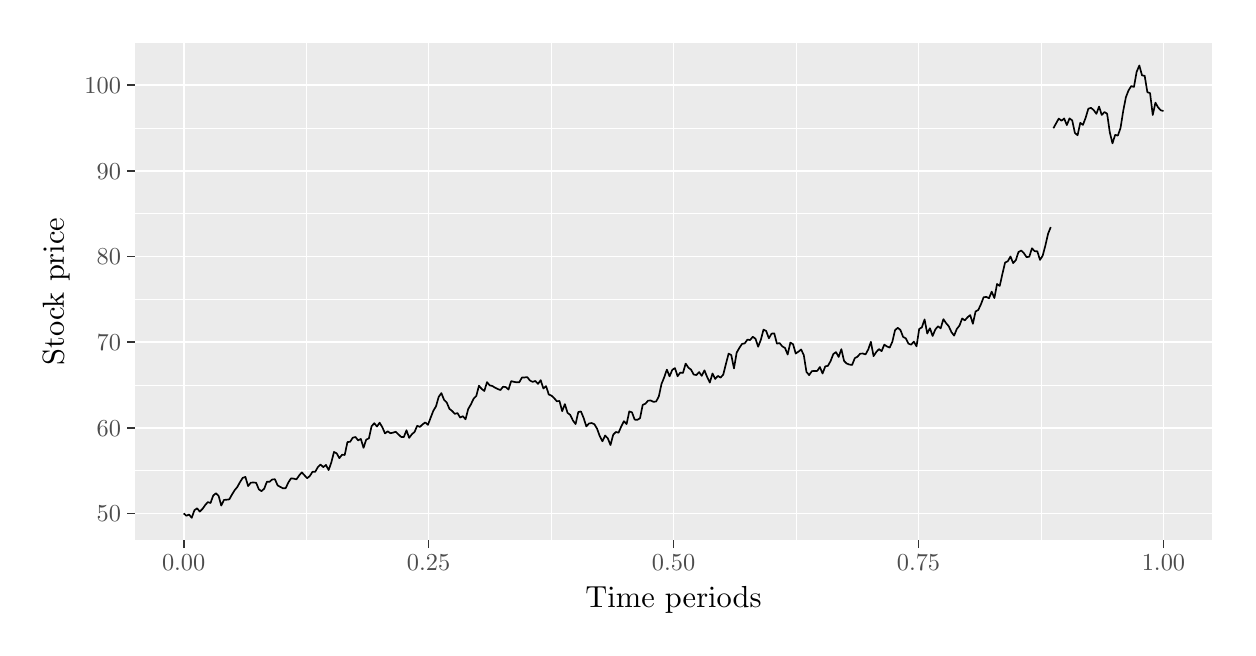
\begin{tikzpicture}[x=1pt,y=1pt]
\definecolor{fillColor}{RGB}{255,255,255}
\path[use as bounding box,fill=fillColor,fill opacity=0.00] (0,0) rectangle (433.62,216.81);
\begin{scope}
\path[clip] (  0.00,  0.00) rectangle (433.62,216.81);
\definecolor{drawColor}{RGB}{255,255,255}
\definecolor{fillColor}{RGB}{255,255,255}

\path[draw=drawColor,line width= 0.6pt,line join=round,line cap=round,fill=fillColor] (  0.00,  0.00) rectangle (433.62,216.81);
\end{scope}
\begin{scope}
\path[clip] ( 38.67, 31.53) rectangle (428.12,211.31);
\definecolor{fillColor}{gray}{0.92}

\path[fill=fillColor] ( 38.67, 31.53) rectangle (428.12,211.31);
\definecolor{drawColor}{RGB}{255,255,255}

\path[draw=drawColor,line width= 0.3pt,line join=round] ( 38.67, 56.77) --
	(428.12, 56.77);

\path[draw=drawColor,line width= 0.3pt,line join=round] ( 38.67, 87.71) --
	(428.12, 87.71);

\path[draw=drawColor,line width= 0.3pt,line join=round] ( 38.67,118.64) --
	(428.12,118.64);

\path[draw=drawColor,line width= 0.3pt,line join=round] ( 38.67,149.58) --
	(428.12,149.58);

\path[draw=drawColor,line width= 0.3pt,line join=round] ( 38.67,180.52) --
	(428.12,180.52);

\path[draw=drawColor,line width= 0.3pt,line join=round] (100.63, 31.53) --
	(100.63,211.31);

\path[draw=drawColor,line width= 0.3pt,line join=round] (189.14, 31.53) --
	(189.14,211.31);

\path[draw=drawColor,line width= 0.3pt,line join=round] (277.65, 31.53) --
	(277.65,211.31);

\path[draw=drawColor,line width= 0.3pt,line join=round] (366.16, 31.53) --
	(366.16,211.31);

\path[draw=drawColor,line width= 0.6pt,line join=round] ( 38.67, 41.30) --
	(428.12, 41.30);

\path[draw=drawColor,line width= 0.6pt,line join=round] ( 38.67, 72.24) --
	(428.12, 72.24);

\path[draw=drawColor,line width= 0.6pt,line join=round] ( 38.67,103.17) --
	(428.12,103.17);

\path[draw=drawColor,line width= 0.6pt,line join=round] ( 38.67,134.11) --
	(428.12,134.11);

\path[draw=drawColor,line width= 0.6pt,line join=round] ( 38.67,165.05) --
	(428.12,165.05);

\path[draw=drawColor,line width= 0.6pt,line join=round] ( 38.67,195.99) --
	(428.12,195.99);

\path[draw=drawColor,line width= 0.6pt,line join=round] ( 56.37, 31.53) --
	( 56.37,211.31);

\path[draw=drawColor,line width= 0.6pt,line join=round] (144.88, 31.53) --
	(144.88,211.31);

\path[draw=drawColor,line width= 0.6pt,line join=round] (233.39, 31.53) --
	(233.39,211.31);

\path[draw=drawColor,line width= 0.6pt,line join=round] (321.91, 31.53) --
	(321.91,211.31);

\path[draw=drawColor,line width= 0.6pt,line join=round] (410.42, 31.53) --
	(410.42,211.31);
\definecolor{drawColor}{RGB}{0,0,0}

\path[draw=drawColor,line width= 0.6pt,line join=round] ( 56.37, 41.30) --
	( 57.34, 40.44) --
	( 58.31, 40.89) --
	( 59.28, 39.70) --
	( 60.25, 42.44) --
	( 61.22, 43.13) --
	( 62.19, 41.95) --
	( 63.16, 42.90) --
	( 64.13, 44.27) --
	( 65.10, 45.39) --
	( 66.07, 45.04) --
	( 67.04, 47.73) --
	( 68.01, 48.55) --
	( 68.98, 47.66) --
	( 69.95, 44.13) --
	( 70.92, 46.15) --
	( 71.89, 46.24) --
	( 72.86, 46.37) --
	( 73.83, 48.12) --
	( 74.80, 49.68) --
	( 75.77, 50.86) --
	( 76.74, 52.62) --
	( 77.71, 54.15) --
	( 78.68, 54.45) --
	( 79.65, 51.16) --
	( 80.62, 52.39) --
	( 81.59, 52.46) --
	( 82.56, 52.36) --
	( 83.53, 49.99) --
	( 84.50, 49.34) --
	( 85.47, 50.22) --
	( 86.44, 52.73) --
	( 87.41, 52.72) --
	( 88.38, 53.56) --
	( 89.35, 53.63) --
	( 90.32, 51.41) --
	( 91.29, 50.86) --
	( 92.26, 50.35) --
	( 93.23, 50.41) --
	( 94.20, 52.47) --
	( 95.17, 53.97) --
	( 96.14, 53.85) --
	( 97.11, 53.58) --
	( 98.08, 54.97) --
	( 99.05, 56.12) --
	(100.02, 55.07) --
	(100.99, 54.00) --
	(101.96, 54.81) --
	(102.93, 56.34) --
	(103.90, 56.31) --
	(104.87, 58.05) --
	(105.84, 58.94) --
	(106.81, 58.01) --
	(107.78, 58.80) --
	(108.75, 56.95) --
	(109.72, 59.70) --
	(110.69, 63.50) --
	(111.66, 63.00) --
	(112.63, 61.26) --
	(113.60, 62.48) --
	(114.57, 62.41) --
	(115.54, 67.06) --
	(116.51, 67.17) --
	(117.48, 68.66) --
	(118.45, 68.90) --
	(119.42, 67.67) --
	(120.39, 68.21) --
	(121.36, 64.99) --
	(122.33, 67.93) --
	(123.30, 68.40) --
	(124.27, 72.77) --
	(125.24, 73.89) --
	(126.21, 72.69) --
	(127.18, 74.07) --
	(128.15, 72.43) --
	(129.12, 70.19) --
	(130.09, 70.94) --
	(131.06, 70.27) --
	(132.03, 70.46) --
	(133.00, 70.79) --
	(133.97, 69.84) --
	(134.94, 68.93) --
	(135.91, 68.86) --
	(136.88, 71.31) --
	(137.85, 68.57) --
	(138.82, 69.89) --
	(139.79, 70.71) --
	(140.76, 72.96) --
	(141.73, 72.55) --
	(142.70, 73.46) --
	(143.67, 74.17) --
	(144.64, 73.30) --
	(145.61, 75.86) --
	(146.58, 78.37) --
	(147.55, 79.97) --
	(148.52, 83.41) --
	(149.49, 84.76) --
	(150.46, 82.33) --
	(151.43, 81.36) --
	(152.40, 79.07) --
	(153.37, 78.31) --
	(154.34, 77.26) --
	(155.31, 77.54) --
	(156.28, 75.91) --
	(157.25, 76.42) --
	(158.22, 75.31) --
	(159.19, 79.03) --
	(160.16, 80.67) --
	(161.13, 82.73) --
	(162.10, 83.72) --
	(163.07, 87.42) --
	(164.04, 86.29) --
	(165.01, 85.53) --
	(165.98, 88.73) --
	(166.95, 87.56) --
	(167.92, 87.33) --
	(168.89, 86.71) --
	(169.86, 86.24) --
	(170.83, 85.86) --
	(171.80, 87.09) --
	(172.77, 86.92) --
	(173.74, 86.06) --
	(174.71, 89.09) --
	(175.68, 88.84) --
	(176.65, 88.66) --
	(177.62, 88.65) --
	(178.59, 90.37) --
	(179.56, 90.42) --
	(180.53, 90.54) --
	(181.50, 89.30) --
	(182.47, 88.81) --
	(183.44, 89.14) --
	(184.41, 88.10) --
	(185.38, 89.43) --
	(186.35, 86.43) --
	(187.32, 87.28) --
	(188.29, 84.27) --
	(189.26, 83.85) --
	(190.23, 82.96) --
	(191.20, 81.82) --
	(192.17, 81.90) --
	(193.14, 78.22) --
	(194.11, 80.79) --
	(195.08, 77.62) --
	(196.05, 76.89) --
	(197.02, 74.87) --
	(197.99, 73.58) --
	(198.96, 77.91) --
	(199.93, 78.13) --
	(200.90, 75.76) --
	(201.87, 72.73) --
	(202.84, 73.79) --
	(203.81, 73.95) --
	(204.78, 73.51) --
	(205.75, 71.89) --
	(206.72, 69.21) --
	(207.69, 67.35) --
	(208.66, 69.43) --
	(209.63, 68.43) --
	(210.60, 65.99) --
	(211.57, 69.72) --
	(212.54, 70.72) --
	(213.51, 70.45) --
	(214.48, 72.69) --
	(215.45, 74.61) --
	(216.42, 73.58) --
	(217.39, 78.14) --
	(218.36, 77.82) --
	(219.33, 75.18) --
	(220.30, 75.09) --
	(221.27, 75.69) --
	(222.24, 80.51) --
	(223.21, 80.92) --
	(224.18, 82.04) --
	(225.15, 82.08) --
	(226.12, 81.60) --
	(227.09, 81.72) --
	(228.06, 83.54) --
	(229.03, 88.06) --
	(230.00, 90.45) --
	(230.97, 93.25) --
	(231.94, 90.81) --
	(232.91, 93.13) --
	(233.88, 93.81) --
	(234.85, 90.86) --
	(235.82, 92.18) --
	(236.79, 92.05) --
	(237.76, 95.43) --
	(238.73, 93.97) --
	(239.70, 93.25) --
	(240.67, 91.46) --
	(241.64, 91.29) --
	(242.61, 92.36) --
	(243.58, 90.99) --
	(244.55, 92.98) --
	(245.52, 90.59) --
	(246.49, 88.57) --
	(247.46, 91.85) --
	(248.43, 89.88) --
	(249.40, 90.97) --
	(250.37, 90.36) --
	(251.34, 91.44) --
	(252.31, 95.30) --
	(253.28, 99.01) --
	(254.25, 98.49) --
	(255.22, 93.69) --
	(256.19, 99.39) --
	(257.16,101.09) --
	(258.13,102.53) --
	(259.10,102.72) --
	(260.07,104.09) --
	(261.04,103.94) --
	(262.01,105.11) --
	(262.98,104.42) --
	(263.95,101.53) --
	(264.92,103.99) --
	(265.89,107.69) --
	(266.86,107.20) --
	(267.83,104.55) --
	(268.80,106.24) --
	(269.77,106.36) --
	(270.74,102.62) --
	(271.71,102.84) --
	(272.68,101.64) --
	(273.65,101.09) --
	(274.62, 98.72) --
	(275.59,102.98) --
	(276.56,102.45) --
	(277.53, 99.06) --
	(278.50, 99.72) --
	(279.47,100.52) --
	(280.44, 98.53) --
	(281.41, 92.43) --
	(282.38, 91.26) --
	(283.35, 92.69) --
	(284.32, 92.77) --
	(285.29, 92.77) --
	(286.26, 94.19) --
	(287.23, 91.83) --
	(288.20, 94.41) --
	(289.17, 94.61) --
	(290.14, 96.36) --
	(291.11, 98.86) --
	(292.08, 99.57) --
	(293.05, 97.83) --
	(294.02,100.64) --
	(294.99, 96.41) --
	(295.96, 95.43) --
	(296.93, 95.08) --
	(297.90, 94.93) --
	(298.87, 97.38) --
	(299.84, 97.89) --
	(300.81, 99.01) --
	(301.78, 99.06) --
	(302.75, 98.73) --
	(303.72,100.49) --
	(304.69,103.29) --
	(305.66, 98.12) --
	(306.63, 99.61) --
	(307.60,100.66) --
	(308.57, 99.92) --
	(309.54,102.27) --
	(310.51,101.61) --
	(311.48,101.19) --
	(312.45,103.34) --
	(313.42,107.50) --
	(314.39,108.35) --
	(315.36,107.59) --
	(316.33,105.08) --
	(317.30,104.54) --
	(318.27,102.63) --
	(319.24,102.26) --
	(320.21,103.37) --
	(321.18,101.66) --
	(322.15,107.93) --
	(323.12,108.51) --
	(324.09,111.38) --
	(325.06,106.28) --
	(326.03,108.21) --
	(327.00,105.40) --
	(327.97,107.74) --
	(328.94,108.89) --
	(329.91,108.16) --
	(330.88,111.48) --
	(331.85,110.06) --
	(332.82,108.93) --
	(333.79,106.83) --
	(334.76,105.52) --
	(335.73,107.92) --
	(336.70,109.15) --
	(337.67,111.73) --
	(338.64,111.04) --
	(339.61,112.15) --
	(340.58,112.95) --
	(341.55,109.82) --
	(342.52,114.25) --
	(343.49,114.80) --
	(344.46,116.86) --
	(345.43,119.41) --
	(346.40,119.52) --
	(347.37,119.01) --
	(348.34,121.43) --
	(349.31,119.10) --
	(350.28,124.19) --
	(351.25,123.48) --
	(352.22,127.86) --
	(353.19,131.95) --
	(354.16,132.41) --
	(355.13,134.13) --
	(356.10,131.73) --
	(357.07,132.81) --
	(358.04,135.76) --
	(359.01,136.27) --
	(359.98,135.34) --
	(360.95,133.89) --
	(361.92,134.04) --
	(362.89,137.08) --
	(363.86,136.06) --
	(364.83,136.00) --
	(365.80,132.89) --
	(366.77,134.42) --
	(367.74,138.09) --
	(368.71,142.31) --
	(369.68,144.76);

\path[draw=drawColor,line width= 0.6pt,line join=round] (370.65,180.47) --
	(371.62,182.25) --
	(372.59,183.97) --
	(373.56,183.17) --
	(374.53,184.00) --
	(375.50,181.61) --
	(376.47,184.02) --
	(377.44,183.30) --
	(378.41,178.76) --
	(379.38,177.93) --
	(380.35,182.42) --
	(381.32,181.68) --
	(382.29,184.25) --
	(383.26,187.52) --
	(384.23,187.84) --
	(385.20,187.03) --
	(386.17,185.67) --
	(387.14,188.30) --
	(388.11,185.26) --
	(389.08,186.33) --
	(390.05,185.72) --
	(391.02,179.01) --
	(391.99,175.01) --
	(392.96,178.09) --
	(393.93,177.80) --
	(394.90,180.55) --
	(395.87,186.72) --
	(396.84,191.69) --
	(397.81,194.17) --
	(398.78,195.71) --
	(399.75,195.39) --
	(400.72,200.85) --
	(401.69,203.14) --
	(402.66,199.59) --
	(403.63,199.39) --
	(404.60,193.48) --
	(405.57,193.16) --
	(406.54,185.25) --
	(407.51,189.70) --
	(408.48,187.99) --
	(409.45,186.94) --
	(410.42,186.71);
\end{scope}
\begin{scope}
\path[clip] (  0.00,  0.00) rectangle (433.62,216.81);
\definecolor{drawColor}{gray}{0.30}

\node[text=drawColor,anchor=base east,inner sep=0pt, outer sep=0pt, scale=  0.88] at ( 33.72, 38.27) {50};

\node[text=drawColor,anchor=base east,inner sep=0pt, outer sep=0pt, scale=  0.88] at ( 33.72, 69.21) {60};

\node[text=drawColor,anchor=base east,inner sep=0pt, outer sep=0pt, scale=  0.88] at ( 33.72,100.14) {70};

\node[text=drawColor,anchor=base east,inner sep=0pt, outer sep=0pt, scale=  0.88] at ( 33.72,131.08) {80};

\node[text=drawColor,anchor=base east,inner sep=0pt, outer sep=0pt, scale=  0.88] at ( 33.72,162.02) {90};

\node[text=drawColor,anchor=base east,inner sep=0pt, outer sep=0pt, scale=  0.88] at ( 33.72,192.96) {100};
\end{scope}
\begin{scope}
\path[clip] (  0.00,  0.00) rectangle (433.62,216.81);
\definecolor{drawColor}{gray}{0.20}

\path[draw=drawColor,line width= 0.6pt,line join=round] ( 35.92, 41.30) --
	( 38.67, 41.30);

\path[draw=drawColor,line width= 0.6pt,line join=round] ( 35.92, 72.24) --
	( 38.67, 72.24);

\path[draw=drawColor,line width= 0.6pt,line join=round] ( 35.92,103.17) --
	( 38.67,103.17);

\path[draw=drawColor,line width= 0.6pt,line join=round] ( 35.92,134.11) --
	( 38.67,134.11);

\path[draw=drawColor,line width= 0.6pt,line join=round] ( 35.92,165.05) --
	( 38.67,165.05);

\path[draw=drawColor,line width= 0.6pt,line join=round] ( 35.92,195.99) --
	( 38.67,195.99);
\end{scope}
\begin{scope}
\path[clip] (  0.00,  0.00) rectangle (433.62,216.81);
\definecolor{drawColor}{gray}{0.20}

\path[draw=drawColor,line width= 0.6pt,line join=round] ( 56.37, 28.78) --
	( 56.37, 31.53);

\path[draw=drawColor,line width= 0.6pt,line join=round] (144.88, 28.78) --
	(144.88, 31.53);

\path[draw=drawColor,line width= 0.6pt,line join=round] (233.39, 28.78) --
	(233.39, 31.53);

\path[draw=drawColor,line width= 0.6pt,line join=round] (321.91, 28.78) --
	(321.91, 31.53);

\path[draw=drawColor,line width= 0.6pt,line join=round] (410.42, 28.78) --
	(410.42, 31.53);
\end{scope}
\begin{scope}
\path[clip] (  0.00,  0.00) rectangle (433.62,216.81);
\definecolor{drawColor}{gray}{0.30}

\node[text=drawColor,anchor=base,inner sep=0pt, outer sep=0pt, scale=  0.88] at ( 56.37, 20.52) {0.00};

\node[text=drawColor,anchor=base,inner sep=0pt, outer sep=0pt, scale=  0.88] at (144.88, 20.52) {0.25};

\node[text=drawColor,anchor=base,inner sep=0pt, outer sep=0pt, scale=  0.88] at (233.39, 20.52) {0.50};

\node[text=drawColor,anchor=base,inner sep=0pt, outer sep=0pt, scale=  0.88] at (321.91, 20.52) {0.75};

\node[text=drawColor,anchor=base,inner sep=0pt, outer sep=0pt, scale=  0.88] at (410.42, 20.52) {1.00};
\end{scope}
\begin{scope}
\path[clip] (  0.00,  0.00) rectangle (433.62,216.81);
\definecolor{drawColor}{RGB}{0,0,0}

\node[text=drawColor,anchor=base,inner sep=0pt, outer sep=0pt, scale=  1.10] at (233.39,  7.44) {Time periods};
\end{scope}
\begin{scope}
\path[clip] (  0.00,  0.00) rectangle (433.62,216.81);
\definecolor{drawColor}{RGB}{0,0,0}

\node[text=drawColor,rotate= 90.00,anchor=base,inner sep=0pt, outer sep=0pt, scale=  1.10] at ( 13.08,121.42) {Stock price};
\end{scope}
\end{tikzpicture}
 
  \floatfoot{Simulation of one Merton mixed jump-diffusion time serie. Data have been output by the R function \textit{sstoch\_jump()} which is an implementation of equation \cref{eq:other:merton:pde} (see appendix \ref{sub:r:time:merton}, for more information). The parameters passed to the function are:  $S(0) = 50$,   $T = 1$ (in year, along with a time step of 365 measures per year),  $\sigma = 0.2$, $\alpha = 0.5$,  $\lambda = 2$,  $\mu = 0.05$, and $\delta = 0.1$.}
  \caption{Merton mixed jump-diffusion time serie}
  \label{p:other:merton:path}
\end{figure}




%%%%%%%%%%%%%%%%%%%%%%%%%%%%%%%%%%%%%%%%%%%%%%%%
% SUBSECTION: Skewness
%%%%%%%%%%%%%%%%%%%%%%%%%%%%%%%%%%%%%%%%%%%%%%%%
\subsection{Impact on the skewness log--return}
\label{sub:MertonSkewness}

The way to influence the direction of the distibution's shape is achieved by moving the cursor of the expected value of jump impact, in other word, by changing the value of the parameter $\mu$. The figure [REF] shows how the density's shape of the log--return may vary along with this parameter.


\begin{figure}[ht]
\centering
% Created by tikzDevice version 0.11 on 2018-04-10 23:12:32
% !TEX encoding = UTF-8 Unicode
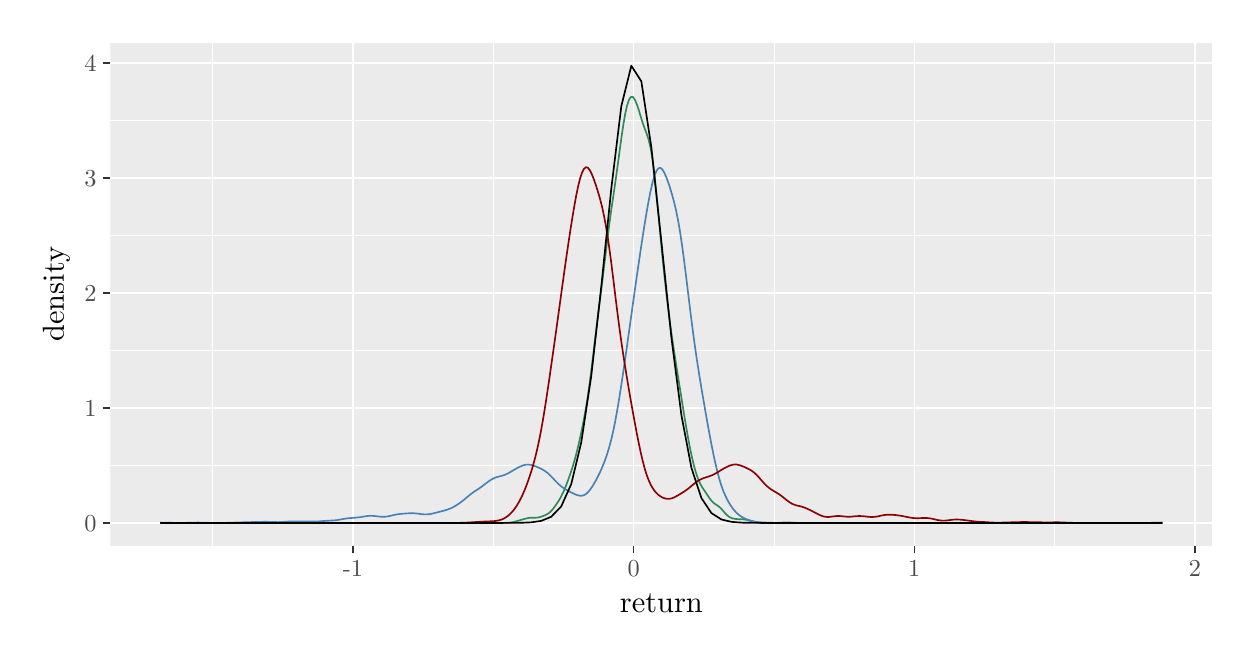
\begin{tikzpicture}[x=1pt,y=1pt]
\definecolor{fillColor}{RGB}{255,255,255}
\path[use as bounding box,fill=fillColor,fill opacity=0.00] (0,0) rectangle (433.62,216.81);
\begin{scope}
\path[clip] (  0.00,  0.00) rectangle (433.62,216.81);
\definecolor{drawColor}{RGB}{255,255,255}
\definecolor{fillColor}{RGB}{255,255,255}

\path[draw=drawColor,line width= 0.6pt,line join=round,line cap=round,fill=fillColor] (  0.00,  0.00) rectangle (433.62,216.81);
\end{scope}
\begin{scope}
\path[clip] ( 29.87, 29.59) rectangle (428.12,211.31);
\definecolor{fillColor}{gray}{0.92}

\path[fill=fillColor] ( 29.87, 29.59) rectangle (428.12,211.31);
\definecolor{drawColor}{RGB}{255,255,255}

\path[draw=drawColor,line width= 0.3pt,line join=round] ( 29.87, 58.62) --
	(428.12, 58.62);

\path[draw=drawColor,line width= 0.3pt,line join=round] ( 29.87,100.17) --
	(428.12,100.17);

\path[draw=drawColor,line width= 0.3pt,line join=round] ( 29.87,141.71) --
	(428.12,141.71);

\path[draw=drawColor,line width= 0.3pt,line join=round] ( 29.87,183.26) --
	(428.12,183.26);

\path[draw=drawColor,line width= 0.3pt,line join=round] ( 66.80, 29.59) --
	( 66.80,211.31);

\path[draw=drawColor,line width= 0.3pt,line join=round] (168.24, 29.59) --
	(168.24,211.31);

\path[draw=drawColor,line width= 0.3pt,line join=round] (269.68, 29.59) --
	(269.68,211.31);

\path[draw=drawColor,line width= 0.3pt,line join=round] (371.11, 29.59) --
	(371.11,211.31);

\path[draw=drawColor,line width= 0.6pt,line join=round] ( 29.87, 37.85) --
	(428.12, 37.85);

\path[draw=drawColor,line width= 0.6pt,line join=round] ( 29.87, 79.39) --
	(428.12, 79.39);

\path[draw=drawColor,line width= 0.6pt,line join=round] ( 29.87,120.94) --
	(428.12,120.94);

\path[draw=drawColor,line width= 0.6pt,line join=round] ( 29.87,162.49) --
	(428.12,162.49);

\path[draw=drawColor,line width= 0.6pt,line join=round] ( 29.87,204.03) --
	(428.12,204.03);

\path[draw=drawColor,line width= 0.6pt,line join=round] (117.52, 29.59) --
	(117.52,211.31);

\path[draw=drawColor,line width= 0.6pt,line join=round] (218.96, 29.59) --
	(218.96,211.31);

\path[draw=drawColor,line width= 0.6pt,line join=round] (320.39, 29.59) --
	(320.39,211.31);

\path[draw=drawColor,line width= 0.6pt,line join=round] (421.83, 29.59) --
	(421.83,211.31);
\definecolor{drawColor}{RGB}{46,139,87}

\path[draw=drawColor,line width= 0.6pt,line join=round] ( 47.97, 37.85) --
	( 48.68, 37.85) --
	( 49.39, 37.85) --
	( 50.10, 37.85) --
	( 50.81, 37.85) --
	( 51.51, 37.85) --
	( 52.22, 37.85) --
	( 52.93, 37.85) --
	( 53.64, 37.85) --
	( 54.35, 37.85) --
	( 55.06, 37.85) --
	( 55.76, 37.85) --
	( 56.47, 37.85) --
	( 57.18, 37.85) --
	( 57.89, 37.85) --
	( 58.60, 37.85) --
	( 59.31, 37.85) --
	( 60.02, 37.85) --
	( 60.72, 37.85) --
	( 61.43, 37.85) --
	( 62.14, 37.85) --
	( 62.85, 37.85) --
	( 63.56, 37.85) --
	( 64.27, 37.85) --
	( 64.98, 37.85) --
	( 65.68, 37.85) --
	( 66.39, 37.85) --
	( 67.10, 37.85) --
	( 67.81, 37.85) --
	( 68.52, 37.85) --
	( 69.23, 37.85) --
	( 69.93, 37.85) --
	( 70.64, 37.85) --
	( 71.35, 37.85) --
	( 72.06, 37.85) --
	( 72.77, 37.85) --
	( 73.48, 37.85) --
	( 74.19, 37.85) --
	( 74.89, 37.85) --
	( 75.60, 37.85) --
	( 76.31, 37.85) --
	( 77.02, 37.85) --
	( 77.73, 37.85) --
	( 78.44, 37.85) --
	( 79.15, 37.85) --
	( 79.85, 37.85) --
	( 80.56, 37.85) --
	( 81.27, 37.85) --
	( 81.98, 37.85) --
	( 82.69, 37.85) --
	( 83.40, 37.85) --
	( 84.10, 37.85) --
	( 84.81, 37.85) --
	( 85.52, 37.85) --
	( 86.23, 37.85) --
	( 86.94, 37.85) --
	( 87.65, 37.85) --
	( 88.36, 37.85) --
	( 89.06, 37.85) --
	( 89.77, 37.85) --
	( 90.48, 37.85) --
	( 91.19, 37.85) --
	( 91.90, 37.85) --
	( 92.61, 37.85) --
	( 93.32, 37.85) --
	( 94.02, 37.85) --
	( 94.73, 37.85) --
	( 95.44, 37.85) --
	( 96.15, 37.85) --
	( 96.86, 37.85) --
	( 97.57, 37.85) --
	( 98.28, 37.85) --
	( 98.98, 37.85) --
	( 99.69, 37.85) --
	(100.40, 37.85) --
	(101.11, 37.85) --
	(101.82, 37.85) --
	(102.53, 37.85) --
	(103.23, 37.85) --
	(103.94, 37.85) --
	(104.65, 37.85) --
	(105.36, 37.85) --
	(106.07, 37.85) --
	(106.78, 37.85) --
	(107.49, 37.85) --
	(108.19, 37.85) --
	(108.90, 37.85) --
	(109.61, 37.85) --
	(110.32, 37.85) --
	(111.03, 37.85) --
	(111.74, 37.85) --
	(112.45, 37.85) --
	(113.15, 37.85) --
	(113.86, 37.85) --
	(114.57, 37.85) --
	(115.28, 37.85) --
	(115.99, 37.85) --
	(116.70, 37.85) --
	(117.40, 37.85) --
	(118.11, 37.85) --
	(118.82, 37.85) --
	(119.53, 37.85) --
	(120.24, 37.85) --
	(120.95, 37.85) --
	(121.66, 37.85) --
	(122.36, 37.85) --
	(123.07, 37.85) --
	(123.78, 37.85) --
	(124.49, 37.85) --
	(125.20, 37.85) --
	(125.91, 37.85) --
	(126.62, 37.85) --
	(127.32, 37.85) --
	(128.03, 37.85) --
	(128.74, 37.85) --
	(129.45, 37.85) --
	(130.16, 37.85) --
	(130.87, 37.85) --
	(131.57, 37.85) --
	(132.28, 37.85) --
	(132.99, 37.85) --
	(133.70, 37.85) --
	(134.41, 37.85) --
	(135.12, 37.85) --
	(135.83, 37.85) --
	(136.53, 37.85) --
	(137.24, 37.85) --
	(137.95, 37.85) --
	(138.66, 37.85) --
	(139.37, 37.85) --
	(140.08, 37.85) --
	(140.79, 37.85) --
	(141.49, 37.85) --
	(142.20, 37.85) --
	(142.91, 37.85) --
	(143.62, 37.85) --
	(144.33, 37.85) --
	(145.04, 37.85) --
	(145.74, 37.85) --
	(146.45, 37.85) --
	(147.16, 37.85) --
	(147.87, 37.85) --
	(148.58, 37.85) --
	(149.29, 37.85) --
	(150.00, 37.85) --
	(150.70, 37.85) --
	(151.41, 37.85) --
	(152.12, 37.85) --
	(152.83, 37.85) --
	(153.54, 37.85) --
	(154.25, 37.85) --
	(154.96, 37.85) --
	(155.66, 37.85) --
	(156.37, 37.85) --
	(157.08, 37.85) --
	(157.79, 37.85) --
	(158.50, 37.86) --
	(159.21, 37.87) --
	(159.92, 37.89) --
	(160.62, 37.93) --
	(161.33, 37.97) --
	(162.04, 38.01) --
	(162.75, 38.03) --
	(163.46, 38.02) --
	(164.17, 38.00) --
	(164.87, 37.96) --
	(165.58, 37.92) --
	(166.29, 37.88) --
	(167.00, 37.86) --
	(167.71, 37.85) --
	(168.42, 37.85) --
	(169.13, 37.85) --
	(169.83, 37.85) --
	(170.54, 37.85) --
	(171.25, 37.85) --
	(171.96, 37.85) --
	(172.67, 37.87) --
	(173.38, 37.89) --
	(174.09, 37.95) --
	(174.79, 38.04) --
	(175.50, 38.18) --
	(176.21, 38.35) --
	(176.92, 38.55) --
	(177.63, 38.76) --
	(178.34, 38.97) --
	(179.04, 39.16) --
	(179.75, 39.35) --
	(180.46, 39.53) --
	(181.17, 39.67) --
	(181.88, 39.74) --
	(182.59, 39.74) --
	(183.30, 39.73) --
	(184.00, 39.76) --
	(184.71, 39.87) --
	(185.42, 40.06) --
	(186.13, 40.31) --
	(186.84, 40.59) --
	(187.55, 40.92) --
	(188.26, 41.35) --
	(188.96, 41.95) --
	(189.67, 42.72) --
	(190.38, 43.64) --
	(191.09, 44.65) --
	(191.80, 45.73) --
	(192.51, 46.92) --
	(193.21, 48.27) --
	(193.92, 49.81) --
	(194.63, 51.56) --
	(195.34, 53.46) --
	(196.05, 55.49) --
	(196.76, 57.64) --
	(197.47, 59.97) --
	(198.17, 62.53) --
	(198.88, 65.35) --
	(199.59, 68.45) --
	(200.30, 71.81) --
	(201.01, 75.44) --
	(201.72, 79.40) --
	(202.43, 83.82) --
	(203.13, 88.81) --
	(203.84, 94.36) --
	(204.55,100.28) --
	(205.26,106.28) --
	(205.97,112.07) --
	(206.68,117.64) --
	(207.39,123.17) --
	(208.09,128.86) --
	(208.80,134.75) --
	(209.51,140.63) --
	(210.22,146.18) --
	(210.93,151.28) --
	(211.64,156.10) --
	(212.34,160.94) --
	(213.05,166.00) --
	(213.76,171.26) --
	(214.47,176.49) --
	(215.18,181.37) --
	(215.89,185.54) --
	(216.60,188.75) --
	(217.30,190.84) --
	(218.01,191.81) --
	(218.72,191.74) --
	(219.43,190.77) --
	(220.14,189.08) --
	(220.85,186.92) --
	(221.56,184.56) --
	(222.26,182.32) --
	(222.97,180.34) --
	(223.68,178.49) --
	(224.39,176.31) --
	(225.10,173.28) --
	(225.81,168.97) --
	(226.51,163.33) --
	(227.22,156.61) --
	(227.93,149.23) --
	(228.64,141.66) --
	(229.35,134.28) --
	(230.06,127.33) --
	(230.77,120.90) --
	(231.47,114.98) --
	(232.18,109.53) --
	(232.89,104.47) --
	(233.60, 99.71) --
	(234.31, 95.15) --
	(235.02, 90.69) --
	(235.73, 86.25) --
	(236.43, 81.81) --
	(237.14, 77.38) --
	(237.85, 73.08) --
	(238.56, 69.00) --
	(239.27, 65.24) --
	(239.98, 61.85) --
	(240.68, 58.86) --
	(241.39, 56.28) --
	(242.10, 54.14) --
	(242.81, 52.43) --
	(243.52, 51.09) --
	(244.23, 49.97) --
	(244.94, 48.94) --
	(245.64, 47.88) --
	(246.35, 46.83) --
	(247.06, 45.89) --
	(247.77, 45.16) --
	(248.48, 44.63) --
	(249.19, 44.18) --
	(249.90, 43.66) --
	(250.60, 42.98) --
	(251.31, 42.18) --
	(252.02, 41.36) --
	(252.73, 40.64) --
	(253.44, 40.08) --
	(254.15, 39.69) --
	(254.85, 39.46) --
	(255.56, 39.32) --
	(256.27, 39.24) --
	(256.98, 39.20) --
	(257.69, 39.18) --
	(258.40, 39.16) --
	(259.11, 39.09) --
	(259.81, 38.96) --
	(260.52, 38.76) --
	(261.23, 38.54) --
	(261.94, 38.31) --
	(262.65, 38.13) --
	(263.36, 38.00) --
	(264.07, 37.92) --
	(264.77, 37.88) --
	(265.48, 37.86) --
	(266.19, 37.85) --
	(266.90, 37.85) --
	(267.61, 37.85) --
	(268.32, 37.85) --
	(269.03, 37.85) --
	(269.73, 37.85) --
	(270.44, 37.87) --
	(271.15, 37.89) --
	(271.86, 37.92) --
	(272.57, 37.96) --
	(273.28, 38.00) --
	(273.98, 38.03) --
	(274.69, 38.03) --
	(275.40, 38.00) --
	(276.11, 37.96) --
	(276.82, 37.92) --
	(277.53, 37.89) --
	(278.24, 37.87) --
	(278.94, 37.85) --
	(279.65, 37.85) --
	(280.36, 37.85) --
	(281.07, 37.85) --
	(281.78, 37.85) --
	(282.49, 37.85) --
	(283.20, 37.85) --
	(283.90, 37.85) --
	(284.61, 37.85) --
	(285.32, 37.85) --
	(286.03, 37.85) --
	(286.74, 37.85) --
	(287.45, 37.85) --
	(288.15, 37.85) --
	(288.86, 37.85) --
	(289.57, 37.85) --
	(290.28, 37.85) --
	(290.99, 37.85) --
	(291.70, 37.85) --
	(292.41, 37.85) --
	(293.11, 37.85) --
	(293.82, 37.85) --
	(294.53, 37.85) --
	(295.24, 37.85) --
	(295.95, 37.85) --
	(296.66, 37.85) --
	(297.37, 37.85) --
	(298.07, 37.85) --
	(298.78, 37.85) --
	(299.49, 37.85) --
	(300.20, 37.85) --
	(300.91, 37.85) --
	(301.62, 37.85) --
	(302.32, 37.85) --
	(303.03, 37.85) --
	(303.74, 37.85) --
	(304.45, 37.85) --
	(305.16, 37.85) --
	(305.87, 37.85) --
	(306.58, 37.85) --
	(307.28, 37.85) --
	(307.99, 37.85) --
	(308.70, 37.85) --
	(309.41, 37.85) --
	(310.12, 37.85) --
	(310.83, 37.85) --
	(311.54, 37.85) --
	(312.24, 37.85) --
	(312.95, 37.85) --
	(313.66, 37.85) --
	(314.37, 37.85) --
	(315.08, 37.85) --
	(315.79, 37.85) --
	(316.49, 37.85) --
	(317.20, 37.85) --
	(317.91, 37.85) --
	(318.62, 37.85) --
	(319.33, 37.85) --
	(320.04, 37.85) --
	(320.75, 37.85) --
	(321.45, 37.85) --
	(322.16, 37.85) --
	(322.87, 37.85) --
	(323.58, 37.85) --
	(324.29, 37.85) --
	(325.00, 37.85) --
	(325.71, 37.85) --
	(326.41, 37.85) --
	(327.12, 37.85) --
	(327.83, 37.85) --
	(328.54, 37.85) --
	(329.25, 37.85) --
	(329.96, 37.85) --
	(330.67, 37.85) --
	(331.37, 37.85) --
	(332.08, 37.85) --
	(332.79, 37.85) --
	(333.50, 37.85) --
	(334.21, 37.85) --
	(334.92, 37.85) --
	(335.62, 37.85) --
	(336.33, 37.85) --
	(337.04, 37.85) --
	(337.75, 37.85) --
	(338.46, 37.85) --
	(339.17, 37.85) --
	(339.88, 37.85) --
	(340.58, 37.85) --
	(341.29, 37.85) --
	(342.00, 37.85) --
	(342.71, 37.85) --
	(343.42, 37.85) --
	(344.13, 37.85) --
	(344.84, 37.85) --
	(345.54, 37.85) --
	(346.25, 37.85) --
	(346.96, 37.85) --
	(347.67, 37.85) --
	(348.38, 37.85) --
	(349.09, 37.85) --
	(349.79, 37.85) --
	(350.50, 37.85) --
	(351.21, 37.85) --
	(351.92, 37.85) --
	(352.63, 37.85) --
	(353.34, 37.85) --
	(354.05, 37.85) --
	(354.75, 37.85) --
	(355.46, 37.85) --
	(356.17, 37.85) --
	(356.88, 37.85) --
	(357.59, 37.85) --
	(358.30, 37.85) --
	(359.01, 37.85) --
	(359.71, 37.85) --
	(360.42, 37.85) --
	(361.13, 37.85) --
	(361.84, 37.85) --
	(362.55, 37.85) --
	(363.26, 37.85) --
	(363.96, 37.85) --
	(364.67, 37.85) --
	(365.38, 37.85) --
	(366.09, 37.85) --
	(366.80, 37.85) --
	(367.51, 37.85) --
	(368.22, 37.85) --
	(368.92, 37.85) --
	(369.63, 37.85) --
	(370.34, 37.85) --
	(371.05, 37.85) --
	(371.76, 37.85) --
	(372.47, 37.85) --
	(373.18, 37.85) --
	(373.88, 37.85) --
	(374.59, 37.85) --
	(375.30, 37.85) --
	(376.01, 37.85) --
	(376.72, 37.85) --
	(377.43, 37.85) --
	(378.13, 37.85) --
	(378.84, 37.85) --
	(379.55, 37.85) --
	(380.26, 37.85) --
	(380.97, 37.85) --
	(381.68, 37.85) --
	(382.39, 37.85) --
	(383.09, 37.85) --
	(383.80, 37.85) --
	(384.51, 37.85) --
	(385.22, 37.85) --
	(385.93, 37.85) --
	(386.64, 37.85) --
	(387.35, 37.85) --
	(388.05, 37.85) --
	(388.76, 37.85) --
	(389.47, 37.85) --
	(390.18, 37.85) --
	(390.89, 37.85) --
	(391.60, 37.85) --
	(392.31, 37.85) --
	(393.01, 37.85) --
	(393.72, 37.85) --
	(394.43, 37.85) --
	(395.14, 37.85) --
	(395.85, 37.85) --
	(396.56, 37.85) --
	(397.26, 37.85) --
	(397.97, 37.85) --
	(398.68, 37.85) --
	(399.39, 37.85) --
	(400.10, 37.85) --
	(400.81, 37.85) --
	(401.52, 37.85) --
	(402.22, 37.85) --
	(402.93, 37.85) --
	(403.64, 37.85) --
	(404.35, 37.85) --
	(405.06, 37.85) --
	(405.77, 37.85) --
	(406.48, 37.85) --
	(407.18, 37.85) --
	(407.89, 37.85) --
	(408.60, 37.85) --
	(409.31, 37.85) --
	(410.02, 37.85);
\definecolor{drawColor}{RGB}{70,130,180}

\path[draw=drawColor,line width= 0.6pt,line join=round] ( 47.97, 37.98) --
	( 48.68, 37.97) --
	( 49.39, 37.96) --
	( 50.10, 37.94) --
	( 50.81, 37.92) --
	( 51.51, 37.90) --
	( 52.22, 37.88) --
	( 52.93, 37.87) --
	( 53.64, 37.86) --
	( 54.35, 37.86) --
	( 55.06, 37.86) --
	( 55.76, 37.86) --
	( 56.47, 37.87) --
	( 57.18, 37.88) --
	( 57.89, 37.90) --
	( 58.60, 37.91) --
	( 59.31, 37.94) --
	( 60.02, 37.96) --
	( 60.72, 37.97) --
	( 61.43, 37.98) --
	( 62.14, 37.97) --
	( 62.85, 37.96) --
	( 63.56, 37.94) --
	( 64.27, 37.92) --
	( 64.98, 37.90) --
	( 65.68, 37.88) --
	( 66.39, 37.87) --
	( 67.10, 37.86) --
	( 67.81, 37.86) --
	( 68.52, 37.85) --
	( 69.23, 37.85) --
	( 69.93, 37.86) --
	( 70.64, 37.86) --
	( 71.35, 37.87) --
	( 72.06, 37.89) --
	( 72.77, 37.91) --
	( 73.48, 37.93) --
	( 74.19, 37.96) --
	( 74.89, 37.98) --
	( 75.60, 38.01) --
	( 76.31, 38.03) --
	( 77.02, 38.05) --
	( 77.73, 38.07) --
	( 78.44, 38.09) --
	( 79.15, 38.12) --
	( 79.85, 38.14) --
	( 80.56, 38.15) --
	( 81.27, 38.17) --
	( 81.98, 38.18) --
	( 82.69, 38.19) --
	( 83.40, 38.20) --
	( 84.10, 38.22) --
	( 84.81, 38.24) --
	( 85.52, 38.26) --
	( 86.23, 38.26) --
	( 86.94, 38.25) --
	( 87.65, 38.23) --
	( 88.36, 38.20) --
	( 89.06, 38.18) --
	( 89.77, 38.16) --
	( 90.48, 38.15) --
	( 91.19, 38.17) --
	( 91.90, 38.20) --
	( 92.61, 38.24) --
	( 93.32, 38.29) --
	( 94.02, 38.33) --
	( 94.73, 38.36) --
	( 95.44, 38.38) --
	( 96.15, 38.39) --
	( 96.86, 38.39) --
	( 97.57, 38.39) --
	( 98.28, 38.40) --
	( 98.98, 38.40) --
	( 99.69, 38.41) --
	(100.40, 38.40) --
	(101.11, 38.39) --
	(101.82, 38.38) --
	(102.53, 38.37) --
	(103.23, 38.36) --
	(103.94, 38.36) --
	(104.65, 38.38) --
	(105.36, 38.42) --
	(106.07, 38.47) --
	(106.78, 38.53) --
	(107.49, 38.58) --
	(108.19, 38.63) --
	(108.90, 38.67) --
	(109.61, 38.70) --
	(110.32, 38.74) --
	(111.03, 38.80) --
	(111.74, 38.88) --
	(112.45, 38.99) --
	(113.15, 39.11) --
	(113.86, 39.24) --
	(114.57, 39.37) --
	(115.28, 39.47) --
	(115.99, 39.56) --
	(116.70, 39.62) --
	(117.40, 39.67) --
	(118.11, 39.72) --
	(118.82, 39.78) --
	(119.53, 39.86) --
	(120.24, 39.95) --
	(120.95, 40.07) --
	(121.66, 40.19) --
	(122.36, 40.30) --
	(123.07, 40.38) --
	(123.78, 40.42) --
	(124.49, 40.41) --
	(125.20, 40.36) --
	(125.91, 40.28) --
	(126.62, 40.19) --
	(127.32, 40.12) --
	(128.03, 40.07) --
	(128.74, 40.07) --
	(129.45, 40.12) --
	(130.16, 40.23) --
	(130.87, 40.37) --
	(131.57, 40.54) --
	(132.28, 40.70) --
	(132.99, 40.86) --
	(133.70, 40.98) --
	(134.41, 41.07) --
	(135.12, 41.14) --
	(135.83, 41.20) --
	(136.53, 41.25) --
	(137.24, 41.30) --
	(137.95, 41.34) --
	(138.66, 41.36) --
	(139.37, 41.34) --
	(140.08, 41.30) --
	(140.79, 41.23) --
	(141.49, 41.14) --
	(142.20, 41.04) --
	(142.91, 40.97) --
	(143.62, 40.93) --
	(144.33, 40.95) --
	(145.04, 41.01) --
	(145.74, 41.12) --
	(146.45, 41.27) --
	(147.16, 41.45) --
	(147.87, 41.63) --
	(148.58, 41.82) --
	(149.29, 42.00) --
	(150.00, 42.18) --
	(150.70, 42.37) --
	(151.41, 42.58) --
	(152.12, 42.83) --
	(152.83, 43.11) --
	(153.54, 43.45) --
	(154.25, 43.83) --
	(154.96, 44.25) --
	(155.66, 44.72) --
	(156.37, 45.22) --
	(157.08, 45.76) --
	(157.79, 46.33) --
	(158.50, 46.92) --
	(159.21, 47.51) --
	(159.92, 48.09) --
	(160.62, 48.63) --
	(161.33, 49.13) --
	(162.04, 49.60) --
	(162.75, 50.06) --
	(163.46, 50.54) --
	(164.17, 51.05) --
	(164.87, 51.59) --
	(165.58, 52.14) --
	(166.29, 52.67) --
	(167.00, 53.17) --
	(167.71, 53.60) --
	(168.42, 53.96) --
	(169.13, 54.25) --
	(169.83, 54.48) --
	(170.54, 54.68) --
	(171.25, 54.87) --
	(171.96, 55.08) --
	(172.67, 55.35) --
	(173.38, 55.67) --
	(174.09, 56.05) --
	(174.79, 56.46) --
	(175.50, 56.88) --
	(176.21, 57.29) --
	(176.92, 57.69) --
	(177.63, 58.06) --
	(178.34, 58.38) --
	(179.04, 58.65) --
	(179.75, 58.84) --
	(180.46, 58.93) --
	(181.17, 58.92) --
	(181.88, 58.81) --
	(182.59, 58.63) --
	(183.30, 58.38) --
	(184.00, 58.11) --
	(184.71, 57.80) --
	(185.42, 57.47) --
	(186.13, 57.09) --
	(186.84, 56.66) --
	(187.55, 56.15) --
	(188.26, 55.56) --
	(188.96, 54.88) --
	(189.67, 54.14) --
	(190.38, 53.37) --
	(191.09, 52.62) --
	(191.80, 51.92) --
	(192.51, 51.29) --
	(193.21, 50.74) --
	(193.92, 50.26) --
	(194.63, 49.83) --
	(195.34, 49.43) --
	(196.05, 49.06) --
	(196.76, 48.69) --
	(197.47, 48.35) --
	(198.17, 48.05) --
	(198.88, 47.82) --
	(199.59, 47.68) --
	(200.30, 47.69) --
	(201.01, 47.88) --
	(201.72, 48.29) --
	(202.43, 48.91) --
	(203.13, 49.74) --
	(203.84, 50.74) --
	(204.55, 51.87) --
	(205.26, 53.11) --
	(205.97, 54.45) --
	(206.68, 55.88) --
	(207.39, 57.44) --
	(208.09, 59.14) --
	(208.80, 61.02) --
	(209.51, 63.12) --
	(210.22, 65.49) --
	(210.93, 68.20) --
	(211.64, 71.28) --
	(212.34, 74.77) --
	(213.05, 78.66) --
	(213.76, 82.91) --
	(214.47, 87.43) --
	(215.18, 92.16) --
	(215.89, 97.03) --
	(216.60,101.99) --
	(217.30,107.01) --
	(218.01,112.07) --
	(218.72,117.14) --
	(219.43,122.19) --
	(220.14,127.18) --
	(220.85,132.08) --
	(221.56,136.87) --
	(222.26,141.52) --
	(222.97,146.01) --
	(223.68,150.28) --
	(224.39,154.27) --
	(225.10,157.86) --
	(225.81,160.94) --
	(226.51,163.38) --
	(227.22,165.09) --
	(227.93,166.01) --
	(228.64,166.16) --
	(229.35,165.57) --
	(230.06,164.38) --
	(230.77,162.75) --
	(231.47,160.83) --
	(232.18,158.68) --
	(232.89,156.32) --
	(233.60,153.69) --
	(234.31,150.69) --
	(235.02,147.18) --
	(235.73,143.08) --
	(236.43,138.36) --
	(237.14,133.10) --
	(237.85,127.45) --
	(238.56,121.61) --
	(239.27,115.78) --
	(239.98,110.13) --
	(240.68,104.76) --
	(241.39, 99.72) --
	(242.10, 94.97) --
	(242.81, 90.49) --
	(243.52, 86.18) --
	(244.23, 82.01) --
	(244.94, 77.92) --
	(245.64, 73.93) --
	(246.35, 70.04) --
	(247.06, 66.30) --
	(247.77, 62.75) --
	(248.48, 59.47) --
	(249.19, 56.48) --
	(249.90, 53.84) --
	(250.60, 51.54) --
	(251.31, 49.55) --
	(252.02, 47.85) --
	(252.73, 46.38) --
	(253.44, 45.11) --
	(254.15, 43.98) --
	(254.85, 42.99) --
	(255.56, 42.13) --
	(256.27, 41.39) --
	(256.98, 40.76) --
	(257.69, 40.25) --
	(258.40, 39.82) --
	(259.11, 39.47) --
	(259.81, 39.17) --
	(260.52, 38.92) --
	(261.23, 38.70) --
	(261.94, 38.51) --
	(262.65, 38.36) --
	(263.36, 38.24) --
	(264.07, 38.15) --
	(264.77, 38.09) --
	(265.48, 38.04) --
	(266.19, 38.00) --
	(266.90, 37.97) --
	(267.61, 37.94) --
	(268.32, 37.91) --
	(269.03, 37.89) --
	(269.73, 37.87) --
	(270.44, 37.86) --
	(271.15, 37.86) --
	(271.86, 37.85) --
	(272.57, 37.85) --
	(273.28, 37.85) --
	(273.98, 37.85) --
	(274.69, 37.85) --
	(275.40, 37.85) --
	(276.11, 37.85) --
	(276.82, 37.85) --
	(277.53, 37.85) --
	(278.24, 37.85) --
	(278.94, 37.85) --
	(279.65, 37.85) --
	(280.36, 37.85) --
	(281.07, 37.85) --
	(281.78, 37.85) --
	(282.49, 37.85) --
	(283.20, 37.85) --
	(283.90, 37.85) --
	(284.61, 37.85) --
	(285.32, 37.85) --
	(286.03, 37.85) --
	(286.74, 37.85) --
	(287.45, 37.85) --
	(288.15, 37.85) --
	(288.86, 37.85) --
	(289.57, 37.85) --
	(290.28, 37.85) --
	(290.99, 37.85) --
	(291.70, 37.85) --
	(292.41, 37.85) --
	(293.11, 37.85) --
	(293.82, 37.85) --
	(294.53, 37.85) --
	(295.24, 37.85) --
	(295.95, 37.85) --
	(296.66, 37.85) --
	(297.37, 37.85) --
	(298.07, 37.85) --
	(298.78, 37.85) --
	(299.49, 37.85) --
	(300.20, 37.85) --
	(300.91, 37.85) --
	(301.62, 37.85) --
	(302.32, 37.85) --
	(303.03, 37.85) --
	(303.74, 37.85) --
	(304.45, 37.85) --
	(305.16, 37.85) --
	(305.87, 37.85) --
	(306.58, 37.85) --
	(307.28, 37.85) --
	(307.99, 37.85) --
	(308.70, 37.85) --
	(309.41, 37.85) --
	(310.12, 37.85) --
	(310.83, 37.85) --
	(311.54, 37.85) --
	(312.24, 37.85) --
	(312.95, 37.85) --
	(313.66, 37.85) --
	(314.37, 37.85) --
	(315.08, 37.85) --
	(315.79, 37.85) --
	(316.49, 37.85) --
	(317.20, 37.85) --
	(317.91, 37.85) --
	(318.62, 37.85) --
	(319.33, 37.85) --
	(320.04, 37.85) --
	(320.75, 37.85) --
	(321.45, 37.85) --
	(322.16, 37.85) --
	(322.87, 37.85) --
	(323.58, 37.85) --
	(324.29, 37.85) --
	(325.00, 37.85) --
	(325.71, 37.85) --
	(326.41, 37.85) --
	(327.12, 37.85) --
	(327.83, 37.85) --
	(328.54, 37.85) --
	(329.25, 37.85) --
	(329.96, 37.85) --
	(330.67, 37.85) --
	(331.37, 37.85) --
	(332.08, 37.85) --
	(332.79, 37.85) --
	(333.50, 37.85) --
	(334.21, 37.85) --
	(334.92, 37.85) --
	(335.62, 37.85) --
	(336.33, 37.85) --
	(337.04, 37.85) --
	(337.75, 37.85) --
	(338.46, 37.85) --
	(339.17, 37.85) --
	(339.88, 37.85) --
	(340.58, 37.85) --
	(341.29, 37.85) --
	(342.00, 37.85) --
	(342.71, 37.85) --
	(343.42, 37.85) --
	(344.13, 37.85) --
	(344.84, 37.85) --
	(345.54, 37.85) --
	(346.25, 37.85) --
	(346.96, 37.85) --
	(347.67, 37.85) --
	(348.38, 37.85) --
	(349.09, 37.85) --
	(349.79, 37.85) --
	(350.50, 37.85) --
	(351.21, 37.85) --
	(351.92, 37.85) --
	(352.63, 37.85) --
	(353.34, 37.85) --
	(354.05, 37.85) --
	(354.75, 37.85) --
	(355.46, 37.85) --
	(356.17, 37.85) --
	(356.88, 37.85) --
	(357.59, 37.85) --
	(358.30, 37.85) --
	(359.01, 37.85) --
	(359.71, 37.85) --
	(360.42, 37.85) --
	(361.13, 37.85) --
	(361.84, 37.85) --
	(362.55, 37.85) --
	(363.26, 37.85) --
	(363.96, 37.85) --
	(364.67, 37.85) --
	(365.38, 37.85) --
	(366.09, 37.85) --
	(366.80, 37.85) --
	(367.51, 37.85) --
	(368.22, 37.85) --
	(368.92, 37.85) --
	(369.63, 37.85) --
	(370.34, 37.85) --
	(371.05, 37.85) --
	(371.76, 37.85) --
	(372.47, 37.85) --
	(373.18, 37.85) --
	(373.88, 37.85) --
	(374.59, 37.85) --
	(375.30, 37.85) --
	(376.01, 37.85) --
	(376.72, 37.85) --
	(377.43, 37.85) --
	(378.13, 37.85) --
	(378.84, 37.85) --
	(379.55, 37.85) --
	(380.26, 37.85) --
	(380.97, 37.85) --
	(381.68, 37.85) --
	(382.39, 37.85) --
	(383.09, 37.85) --
	(383.80, 37.85) --
	(384.51, 37.85) --
	(385.22, 37.85) --
	(385.93, 37.85) --
	(386.64, 37.85) --
	(387.35, 37.85) --
	(388.05, 37.85) --
	(388.76, 37.85) --
	(389.47, 37.85) --
	(390.18, 37.85) --
	(390.89, 37.85) --
	(391.60, 37.85) --
	(392.31, 37.85) --
	(393.01, 37.85) --
	(393.72, 37.85) --
	(394.43, 37.85) --
	(395.14, 37.85) --
	(395.85, 37.85) --
	(396.56, 37.85) --
	(397.26, 37.85) --
	(397.97, 37.85) --
	(398.68, 37.85) --
	(399.39, 37.85) --
	(400.10, 37.85) --
	(400.81, 37.85) --
	(401.52, 37.85) --
	(402.22, 37.85) --
	(402.93, 37.85) --
	(403.64, 37.85) --
	(404.35, 37.85) --
	(405.06, 37.85) --
	(405.77, 37.85) --
	(406.48, 37.85) --
	(407.18, 37.85) --
	(407.89, 37.85) --
	(408.60, 37.85) --
	(409.31, 37.85) --
	(410.02, 37.85);
\definecolor{drawColor}{RGB}{139,0,0}

\path[draw=drawColor,line width= 0.6pt,line join=round] ( 47.97, 37.85) --
	( 48.68, 37.85) --
	( 49.39, 37.85) --
	( 50.10, 37.85) --
	( 50.81, 37.85) --
	( 51.51, 37.85) --
	( 52.22, 37.85) --
	( 52.93, 37.85) --
	( 53.64, 37.85) --
	( 54.35, 37.85) --
	( 55.06, 37.85) --
	( 55.76, 37.85) --
	( 56.47, 37.85) --
	( 57.18, 37.85) --
	( 57.89, 37.85) --
	( 58.60, 37.85) --
	( 59.31, 37.85) --
	( 60.02, 37.85) --
	( 60.72, 37.85) --
	( 61.43, 37.85) --
	( 62.14, 37.85) --
	( 62.85, 37.85) --
	( 63.56, 37.85) --
	( 64.27, 37.85) --
	( 64.98, 37.85) --
	( 65.68, 37.85) --
	( 66.39, 37.85) --
	( 67.10, 37.85) --
	( 67.81, 37.85) --
	( 68.52, 37.85) --
	( 69.23, 37.85) --
	( 69.93, 37.85) --
	( 70.64, 37.85) --
	( 71.35, 37.85) --
	( 72.06, 37.85) --
	( 72.77, 37.85) --
	( 73.48, 37.85) --
	( 74.19, 37.85) --
	( 74.89, 37.85) --
	( 75.60, 37.85) --
	( 76.31, 37.85) --
	( 77.02, 37.85) --
	( 77.73, 37.85) --
	( 78.44, 37.85) --
	( 79.15, 37.85) --
	( 79.85, 37.85) --
	( 80.56, 37.85) --
	( 81.27, 37.85) --
	( 81.98, 37.85) --
	( 82.69, 37.85) --
	( 83.40, 37.85) --
	( 84.10, 37.85) --
	( 84.81, 37.85) --
	( 85.52, 37.85) --
	( 86.23, 37.85) --
	( 86.94, 37.85) --
	( 87.65, 37.85) --
	( 88.36, 37.85) --
	( 89.06, 37.85) --
	( 89.77, 37.85) --
	( 90.48, 37.85) --
	( 91.19, 37.85) --
	( 91.90, 37.85) --
	( 92.61, 37.85) --
	( 93.32, 37.85) --
	( 94.02, 37.85) --
	( 94.73, 37.85) --
	( 95.44, 37.85) --
	( 96.15, 37.85) --
	( 96.86, 37.85) --
	( 97.57, 37.85) --
	( 98.28, 37.85) --
	( 98.98, 37.85) --
	( 99.69, 37.85) --
	(100.40, 37.85) --
	(101.11, 37.85) --
	(101.82, 37.85) --
	(102.53, 37.85) --
	(103.23, 37.85) --
	(103.94, 37.85) --
	(104.65, 37.85) --
	(105.36, 37.85) --
	(106.07, 37.85) --
	(106.78, 37.85) --
	(107.49, 37.85) --
	(108.19, 37.85) --
	(108.90, 37.85) --
	(109.61, 37.85) --
	(110.32, 37.85) --
	(111.03, 37.85) --
	(111.74, 37.85) --
	(112.45, 37.85) --
	(113.15, 37.85) --
	(113.86, 37.85) --
	(114.57, 37.85) --
	(115.28, 37.85) --
	(115.99, 37.85) --
	(116.70, 37.85) --
	(117.40, 37.85) --
	(118.11, 37.85) --
	(118.82, 37.85) --
	(119.53, 37.85) --
	(120.24, 37.85) --
	(120.95, 37.85) --
	(121.66, 37.85) --
	(122.36, 37.85) --
	(123.07, 37.85) --
	(123.78, 37.85) --
	(124.49, 37.85) --
	(125.20, 37.85) --
	(125.91, 37.85) --
	(126.62, 37.85) --
	(127.32, 37.85) --
	(128.03, 37.85) --
	(128.74, 37.85) --
	(129.45, 37.85) --
	(130.16, 37.85) --
	(130.87, 37.85) --
	(131.57, 37.85) --
	(132.28, 37.85) --
	(132.99, 37.85) --
	(133.70, 37.85) --
	(134.41, 37.85) --
	(135.12, 37.85) --
	(135.83, 37.85) --
	(136.53, 37.85) --
	(137.24, 37.85) --
	(137.95, 37.85) --
	(138.66, 37.85) --
	(139.37, 37.85) --
	(140.08, 37.85) --
	(140.79, 37.85) --
	(141.49, 37.85) --
	(142.20, 37.85) --
	(142.91, 37.85) --
	(143.62, 37.85) --
	(144.33, 37.85) --
	(145.04, 37.85) --
	(145.74, 37.85) --
	(146.45, 37.85) --
	(147.16, 37.85) --
	(147.87, 37.85) --
	(148.58, 37.85) --
	(149.29, 37.85) --
	(150.00, 37.85) --
	(150.70, 37.85) --
	(151.41, 37.85) --
	(152.12, 37.85) --
	(152.83, 37.85) --
	(153.54, 37.85) --
	(154.25, 37.85) --
	(154.96, 37.86) --
	(155.66, 37.87) --
	(156.37, 37.89) --
	(157.08, 37.91) --
	(157.79, 37.94) --
	(158.50, 37.97) --
	(159.21, 38.00) --
	(159.92, 38.04) --
	(160.62, 38.08) --
	(161.33, 38.13) --
	(162.04, 38.17) --
	(162.75, 38.22) --
	(163.46, 38.27) --
	(164.17, 38.31) --
	(164.87, 38.34) --
	(165.58, 38.37) --
	(166.29, 38.40) --
	(167.00, 38.42) --
	(167.71, 38.45) --
	(168.42, 38.50) --
	(169.13, 38.57) --
	(169.83, 38.69) --
	(170.54, 38.85) --
	(171.25, 39.08) --
	(171.96, 39.38) --
	(172.67, 39.78) --
	(173.38, 40.27) --
	(174.09, 40.86) --
	(174.79, 41.56) --
	(175.50, 42.37) --
	(176.21, 43.31) --
	(176.92, 44.39) --
	(177.63, 45.60) --
	(178.34, 46.97) --
	(179.04, 48.49) --
	(179.75, 50.17) --
	(180.46, 52.01) --
	(181.17, 54.01) --
	(181.88, 56.17) --
	(182.59, 58.53) --
	(183.30, 61.12) --
	(184.00, 63.99) --
	(184.71, 67.20) --
	(185.42, 70.77) --
	(186.13, 74.72) --
	(186.84, 79.01) --
	(187.55, 83.58) --
	(188.26, 88.33) --
	(188.96, 93.19) --
	(189.67, 98.14) --
	(190.38,103.15) --
	(191.09,108.22) --
	(191.80,113.35) --
	(192.51,118.51) --
	(193.21,123.65) --
	(193.92,128.74) --
	(194.63,133.73) --
	(195.34,138.58) --
	(196.05,143.27) --
	(196.76,147.77) --
	(197.47,152.01) --
	(198.17,155.91) --
	(198.88,159.36) --
	(199.59,162.23) --
	(200.30,164.40) --
	(201.01,165.80) --
	(201.72,166.39) --
	(202.43,166.20) --
	(203.13,165.30) --
	(203.84,163.88) --
	(204.55,162.09) --
	(205.26,160.06) --
	(205.97,157.85) --
	(206.68,155.44) --
	(207.39,152.75) --
	(208.09,149.63) --
	(208.80,145.96) --
	(209.51,141.68) --
	(210.22,136.79) --
	(210.93,131.41) --
	(211.64,125.72) --
	(212.34,119.93) --
	(213.05,114.24) --
	(213.76,108.80) --
	(214.47,103.66) --
	(215.18, 98.84) --
	(215.89, 94.28) --
	(216.60, 89.94) --
	(217.30, 85.75) --
	(218.01, 81.66) --
	(218.72, 77.67) --
	(219.43, 73.78) --
	(220.14, 70.03) --
	(220.85, 66.47) --
	(221.56, 63.15) --
	(222.26, 60.14) --
	(222.97, 57.48) --
	(223.68, 55.20) --
	(224.39, 53.29) --
	(225.10, 51.73) --
	(225.81, 50.47) --
	(226.51, 49.45) --
	(227.22, 48.64) --
	(227.93, 47.98) --
	(228.64, 47.45) --
	(229.35, 47.05) --
	(230.06, 46.77) --
	(230.77, 46.59) --
	(231.47, 46.54) --
	(232.18, 46.61) --
	(232.89, 46.79) --
	(233.60, 47.08) --
	(234.31, 47.44) --
	(235.02, 47.84) --
	(235.73, 48.27) --
	(236.43, 48.70) --
	(237.14, 49.15) --
	(237.85, 49.63) --
	(238.56, 50.15) --
	(239.27, 50.71) --
	(239.98, 51.30) --
	(240.68, 51.89) --
	(241.39, 52.45) --
	(242.10, 52.96) --
	(242.81, 53.39) --
	(243.52, 53.75) --
	(244.23, 54.03) --
	(244.94, 54.28) --
	(245.64, 54.49) --
	(246.35, 54.72) --
	(247.06, 54.99) --
	(247.77, 55.31) --
	(248.48, 55.68) --
	(249.19, 56.09) --
	(249.90, 56.53) --
	(250.60, 56.96) --
	(251.31, 57.37) --
	(252.02, 57.77) --
	(252.73, 58.13) --
	(253.44, 58.46) --
	(254.15, 58.72) --
	(254.85, 58.90) --
	(255.56, 58.97) --
	(256.27, 58.93) --
	(256.98, 58.78) --
	(257.69, 58.57) --
	(258.40, 58.30) --
	(259.11, 58.00) --
	(259.81, 57.67) --
	(260.52, 57.32) --
	(261.23, 56.92) --
	(261.94, 56.46) --
	(262.65, 55.90) --
	(263.36, 55.24) --
	(264.07, 54.50) --
	(264.77, 53.69) --
	(265.48, 52.87) --
	(266.19, 52.07) --
	(266.90, 51.35) --
	(267.61, 50.73) --
	(268.32, 50.19) --
	(269.03, 49.73) --
	(269.73, 49.31) --
	(270.44, 48.89) --
	(271.15, 48.45) --
	(271.86, 47.97) --
	(272.57, 47.45) --
	(273.28, 46.89) --
	(273.98, 46.31) --
	(274.69, 45.76) --
	(275.40, 45.26) --
	(276.11, 44.83) --
	(276.82, 44.50) --
	(277.53, 44.26) --
	(278.24, 44.08) --
	(278.94, 43.92) --
	(279.65, 43.74) --
	(280.36, 43.51) --
	(281.07, 43.24) --
	(281.78, 42.93) --
	(282.49, 42.60) --
	(283.20, 42.25) --
	(283.90, 41.89) --
	(284.61, 41.52) --
	(285.32, 41.15) --
	(286.03, 40.80) --
	(286.74, 40.49) --
	(287.45, 40.24) --
	(288.15, 40.08) --
	(288.86, 40.01) --
	(289.57, 40.02) --
	(290.28, 40.09) --
	(290.99, 40.19) --
	(291.70, 40.28) --
	(292.41, 40.34) --
	(293.11, 40.35) --
	(293.82, 40.31) --
	(294.53, 40.24) --
	(295.24, 40.16) --
	(295.95, 40.11) --
	(296.66, 40.08) --
	(297.37, 40.11) --
	(298.07, 40.16) --
	(298.78, 40.23) --
	(299.49, 40.29) --
	(300.20, 40.33) --
	(300.91, 40.33) --
	(301.62, 40.29) --
	(302.32, 40.23) --
	(303.03, 40.15) --
	(303.74, 40.07) --
	(304.45, 40.02) --
	(305.16, 40.00) --
	(305.87, 40.03) --
	(306.58, 40.11) --
	(307.28, 40.24) --
	(307.99, 40.39) --
	(308.70, 40.55) --
	(309.41, 40.68) --
	(310.12, 40.77) --
	(310.83, 40.82) --
	(311.54, 40.83) --
	(312.24, 40.80) --
	(312.95, 40.75) --
	(313.66, 40.69) --
	(314.37, 40.60) --
	(315.08, 40.50) --
	(315.79, 40.39) --
	(316.49, 40.25) --
	(317.20, 40.11) --
	(317.91, 39.96) --
	(318.62, 39.82) --
	(319.33, 39.70) --
	(320.04, 39.61) --
	(320.75, 39.56) --
	(321.45, 39.55) --
	(322.16, 39.57) --
	(322.87, 39.60) --
	(323.58, 39.63) --
	(324.29, 39.64) --
	(325.00, 39.62) --
	(325.71, 39.55) --
	(326.41, 39.44) --
	(327.12, 39.29) --
	(327.83, 39.13) --
	(328.54, 38.96) --
	(329.25, 38.82) --
	(329.96, 38.72) --
	(330.67, 38.67) --
	(331.37, 38.68) --
	(332.08, 38.74) --
	(332.79, 38.83) --
	(333.50, 38.92) --
	(334.21, 39.01) --
	(334.92, 39.06) --
	(335.62, 39.08) --
	(336.33, 39.07) --
	(337.04, 39.02) --
	(337.75, 38.96) --
	(338.46, 38.88) --
	(339.17, 38.79) --
	(339.88, 38.69) --
	(340.58, 38.60) --
	(341.29, 38.50) --
	(342.00, 38.41) --
	(342.71, 38.34) --
	(343.42, 38.28) --
	(344.13, 38.24) --
	(344.84, 38.20) --
	(345.54, 38.17) --
	(346.25, 38.13) --
	(346.96, 38.09) --
	(347.67, 38.04) --
	(348.38, 38.00) --
	(349.09, 37.97) --
	(349.79, 37.95) --
	(350.50, 37.94) --
	(351.21, 37.95) --
	(351.92, 37.97) --
	(352.63, 37.99) --
	(353.34, 38.01) --
	(354.05, 38.03) --
	(354.75, 38.05) --
	(355.46, 38.07) --
	(356.17, 38.09) --
	(356.88, 38.11) --
	(357.59, 38.13) --
	(358.30, 38.15) --
	(359.01, 38.16) --
	(359.71, 38.16) --
	(360.42, 38.16) --
	(361.13, 38.16) --
	(361.84, 38.15) --
	(362.55, 38.15) --
	(363.26, 38.15) --
	(363.96, 38.14) --
	(364.67, 38.13) --
	(365.38, 38.10) --
	(366.09, 38.08) --
	(366.80, 38.05) --
	(367.51, 38.04) --
	(368.22, 38.03) --
	(368.92, 38.03) --
	(369.63, 38.04) --
	(370.34, 38.06) --
	(371.05, 38.07) --
	(371.76, 38.07) --
	(372.47, 38.07) --
	(373.18, 38.06) --
	(373.88, 38.03) --
	(374.59, 38.00) --
	(375.30, 37.97) --
	(376.01, 37.94) --
	(376.72, 37.91) --
	(377.43, 37.89) --
	(378.13, 37.87) --
	(378.84, 37.86) --
	(379.55, 37.86) --
	(380.26, 37.85) --
	(380.97, 37.85) --
	(381.68, 37.85) --
	(382.39, 37.85) --
	(383.09, 37.85) --
	(383.80, 37.85) --
	(384.51, 37.85) --
	(385.22, 37.85) --
	(385.93, 37.85) --
	(386.64, 37.85) --
	(387.35, 37.85) --
	(388.05, 37.85) --
	(388.76, 37.85) --
	(389.47, 37.85) --
	(390.18, 37.85) --
	(390.89, 37.85) --
	(391.60, 37.85) --
	(392.31, 37.85) --
	(393.01, 37.85) --
	(393.72, 37.85) --
	(394.43, 37.85) --
	(395.14, 37.85) --
	(395.85, 37.85) --
	(396.56, 37.85) --
	(397.26, 37.85) --
	(397.97, 37.85) --
	(398.68, 37.85) --
	(399.39, 37.85) --
	(400.10, 37.85) --
	(400.81, 37.85) --
	(401.52, 37.85) --
	(402.22, 37.85) --
	(402.93, 37.85) --
	(403.64, 37.85) --
	(404.35, 37.86) --
	(405.06, 37.87) --
	(405.77, 37.88) --
	(406.48, 37.90) --
	(407.18, 37.92) --
	(407.89, 37.94) --
	(408.60, 37.96) --
	(409.31, 37.97) --
	(410.02, 37.98);
\definecolor{drawColor}{RGB}{0,0,0}

\path[draw=drawColor,line width= 0.6pt,line join=round] ( 47.97, 37.85) --
	( 51.59, 37.85) --
	( 55.21, 37.85) --
	( 58.83, 37.85) --
	( 62.45, 37.85) --
	( 66.07, 37.85) --
	( 69.69, 37.85) --
	( 73.31, 37.85) --
	( 76.93, 37.85) --
	( 80.56, 37.85) --
	( 84.18, 37.85) --
	( 87.80, 37.85) --
	( 91.42, 37.85) --
	( 95.04, 37.85) --
	( 98.66, 37.85) --
	(102.28, 37.85) --
	(105.90, 37.85) --
	(109.52, 37.85) --
	(113.14, 37.85) --
	(116.76, 37.85) --
	(120.38, 37.85) --
	(124.00, 37.85) --
	(127.62, 37.85) --
	(131.24, 37.85) --
	(134.86, 37.85) --
	(138.48, 37.85) --
	(142.10, 37.85) --
	(145.72, 37.85) --
	(149.34, 37.85) --
	(152.96, 37.85) --
	(156.59, 37.85) --
	(160.21, 37.85) --
	(163.83, 37.85) --
	(167.45, 37.85) --
	(171.07, 37.85) --
	(174.69, 37.86) --
	(178.31, 37.90) --
	(181.93, 38.06) --
	(185.55, 38.58) --
	(189.17, 40.07) --
	(192.79, 43.80) --
	(196.41, 51.86) --
	(200.03, 66.92) --
	(203.65, 90.94) --
	(207.27,123.21) --
	(210.89,158.68) --
	(214.51,188.43) --
	(218.13,203.05) --
	(221.75,197.41) --
	(225.37,173.54) --
	(228.99,139.43) --
	(232.61,104.80) --
	(236.24, 76.70) --
	(239.86, 57.69) --
	(243.48, 46.77) --
	(247.10, 41.38) --
	(250.72, 39.08) --
	(254.34, 38.23) --
	(257.96, 37.95) --
	(261.58, 37.87) --
	(265.20, 37.85) --
	(268.82, 37.85) --
	(272.44, 37.85) --
	(276.06, 37.85) --
	(279.68, 37.85) --
	(283.30, 37.85) --
	(286.92, 37.85) --
	(290.54, 37.85) --
	(294.16, 37.85) --
	(297.78, 37.85) --
	(301.40, 37.85) --
	(305.02, 37.85) --
	(308.64, 37.85) --
	(312.27, 37.85) --
	(315.89, 37.85) --
	(319.51, 37.85) --
	(323.13, 37.85) --
	(326.75, 37.85) --
	(330.37, 37.85) --
	(333.99, 37.85) --
	(337.61, 37.85) --
	(341.23, 37.85) --
	(344.85, 37.85) --
	(348.47, 37.85) --
	(352.09, 37.85) --
	(355.71, 37.85) --
	(359.33, 37.85) --
	(362.95, 37.85) --
	(366.57, 37.85) --
	(370.19, 37.85) --
	(373.81, 37.85) --
	(377.43, 37.85) --
	(381.05, 37.85) --
	(384.67, 37.85) --
	(388.29, 37.85) --
	(391.92, 37.85) --
	(395.54, 37.85) --
	(399.16, 37.85) --
	(402.78, 37.85) --
	(406.40, 37.85) --
	(410.02, 37.85);
\end{scope}
\begin{scope}
\path[clip] (  0.00,  0.00) rectangle (433.62,216.81);
\definecolor{drawColor}{gray}{0.30}

\node[text=drawColor,anchor=base east,inner sep=0pt, outer sep=0pt, scale=  0.88] at ( 24.92, 34.82) {0};

\node[text=drawColor,anchor=base east,inner sep=0pt, outer sep=0pt, scale=  0.88] at ( 24.92, 76.36) {1};

\node[text=drawColor,anchor=base east,inner sep=0pt, outer sep=0pt, scale=  0.88] at ( 24.92,117.91) {2};

\node[text=drawColor,anchor=base east,inner sep=0pt, outer sep=0pt, scale=  0.88] at ( 24.92,159.46) {3};

\node[text=drawColor,anchor=base east,inner sep=0pt, outer sep=0pt, scale=  0.88] at ( 24.92,201.00) {4};
\end{scope}
\begin{scope}
\path[clip] (  0.00,  0.00) rectangle (433.62,216.81);
\definecolor{drawColor}{gray}{0.20}

\path[draw=drawColor,line width= 0.6pt,line join=round] ( 27.12, 37.85) --
	( 29.87, 37.85);

\path[draw=drawColor,line width= 0.6pt,line join=round] ( 27.12, 79.39) --
	( 29.87, 79.39);

\path[draw=drawColor,line width= 0.6pt,line join=round] ( 27.12,120.94) --
	( 29.87,120.94);

\path[draw=drawColor,line width= 0.6pt,line join=round] ( 27.12,162.49) --
	( 29.87,162.49);

\path[draw=drawColor,line width= 0.6pt,line join=round] ( 27.12,204.03) --
	( 29.87,204.03);
\end{scope}
\begin{scope}
\path[clip] (  0.00,  0.00) rectangle (433.62,216.81);
\definecolor{drawColor}{gray}{0.20}

\path[draw=drawColor,line width= 0.6pt,line join=round] (117.52, 26.84) --
	(117.52, 29.59);

\path[draw=drawColor,line width= 0.6pt,line join=round] (218.96, 26.84) --
	(218.96, 29.59);

\path[draw=drawColor,line width= 0.6pt,line join=round] (320.39, 26.84) --
	(320.39, 29.59);

\path[draw=drawColor,line width= 0.6pt,line join=round] (421.83, 26.84) --
	(421.83, 29.59);
\end{scope}
\begin{scope}
\path[clip] (  0.00,  0.00) rectangle (433.62,216.81);
\definecolor{drawColor}{gray}{0.30}

\node[text=drawColor,anchor=base,inner sep=0pt, outer sep=0pt, scale=  0.88] at (117.52, 18.58) {-1};

\node[text=drawColor,anchor=base,inner sep=0pt, outer sep=0pt, scale=  0.88] at (218.96, 18.58) {0};

\node[text=drawColor,anchor=base,inner sep=0pt, outer sep=0pt, scale=  0.88] at (320.39, 18.58) {1};

\node[text=drawColor,anchor=base,inner sep=0pt, outer sep=0pt, scale=  0.88] at (421.83, 18.58) {2};
\end{scope}
\begin{scope}
\path[clip] (  0.00,  0.00) rectangle (433.62,216.81);
\definecolor{drawColor}{RGB}{0,0,0}

\node[text=drawColor,anchor=base,inner sep=0pt, outer sep=0pt, scale=  1.10] at (228.99,  5.50) {return};
\end{scope}
\begin{scope}
\path[clip] (  0.00,  0.00) rectangle (433.62,216.81);
\definecolor{drawColor}{RGB}{0,0,0}

\node[text=drawColor,rotate= 90.00,anchor=base,inner sep=0pt, outer sep=0pt, scale=  1.10] at ( 13.08,120.45) {density};
\end{scope}
\end{tikzpicture}

\caption{Merton: Daily Basis Stock Return Density}
\floatfoot{
The above density function has been constructed over three distinctive groups of 5000 samples eachs. All samples have been constructed following \cref{eq:other:merton:pde}. The only parameter that changes over the group is $\mu$ which is set to ($-0.5$, $0$, $0.5$) respectively for the blue, green and red density function. The black density belongs to the normal curve with mean 0 and standard deviation of $\sqrt{dt} \times \sigma$. 
}
\label{plot:MertonReturnDensity}
\end{figure}

%%%%%%%%%%%%%%%%%%%%%%%%%%%%%%%%%%%%%%%%%%%%%%%%
% SUBSECTION: kurtosis
%%%%%%%%%%%%%%%%%%%%%%%%%%%%%%%%%%%%%%%%%%%%%%%%
\subsection{Impact on kurtosis log--return}
\label{sub:MertonKurtosis}

The way to influence the aspect of the distibution's tails is achieved by moving the cursor of the expected value of jump occurence, in other word, by changing the value of the parameter $\lambda$. The \cref{p:MertonReturnDensityTails} shows how the distribution's tails of the log--return may vary along with this parameter.

\begin{figure}[ht]
\centering
% Created by tikzDevice version 0.11 on 2018-04-10 23:11:48
% !TEX encoding = UTF-8 Unicode
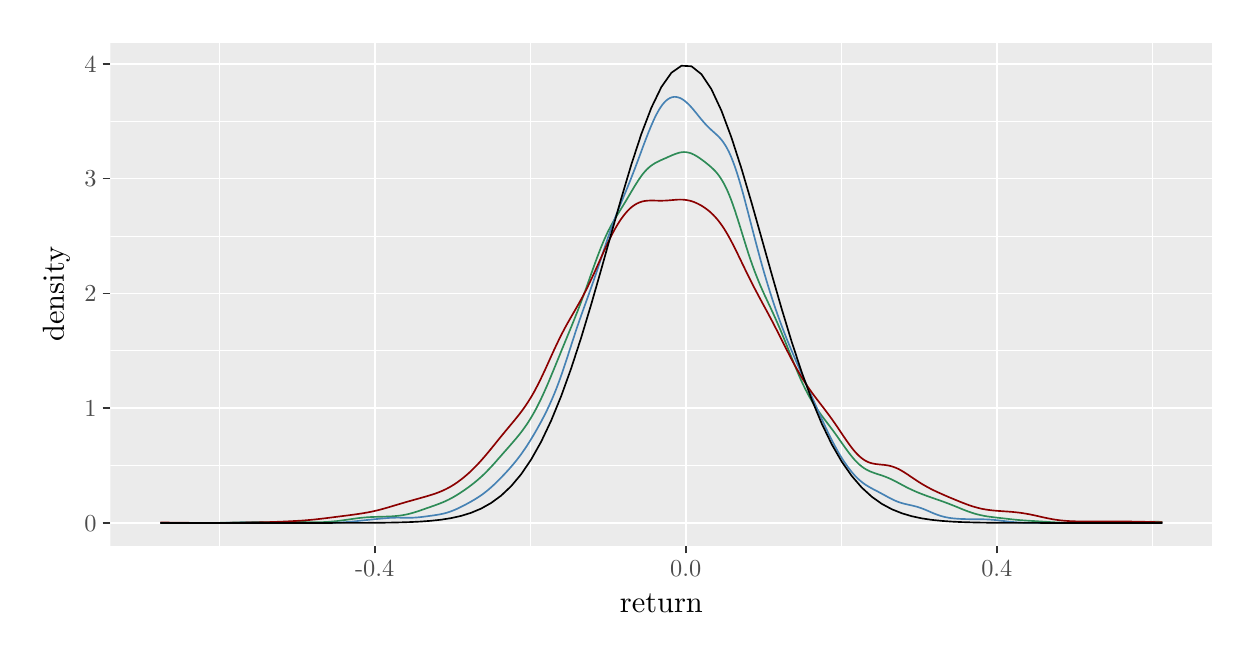
\begin{tikzpicture}[x=1pt,y=1pt]
\definecolor{fillColor}{RGB}{255,255,255}
\path[use as bounding box,fill=fillColor,fill opacity=0.00] (0,0) rectangle (433.62,216.81);
\begin{scope}
\path[clip] (  0.00,  0.00) rectangle (433.62,216.81);
\definecolor{drawColor}{RGB}{255,255,255}
\definecolor{fillColor}{RGB}{255,255,255}

\path[draw=drawColor,line width= 0.6pt,line join=round,line cap=round,fill=fillColor] (  0.00,  0.00) rectangle (433.62,216.81);
\end{scope}
\begin{scope}
\path[clip] ( 29.87, 29.59) rectangle (428.12,211.31);
\definecolor{fillColor}{gray}{0.92}

\path[fill=fillColor] ( 29.87, 29.59) rectangle (428.12,211.31);
\definecolor{drawColor}{RGB}{255,255,255}

\path[draw=drawColor,line width= 0.3pt,line join=round] ( 29.87, 58.58) --
	(428.12, 58.58);

\path[draw=drawColor,line width= 0.3pt,line join=round] ( 29.87,100.06) --
	(428.12,100.06);

\path[draw=drawColor,line width= 0.3pt,line join=round] ( 29.87,141.53) --
	(428.12,141.53);

\path[draw=drawColor,line width= 0.3pt,line join=round] ( 29.87,183.01) --
	(428.12,183.01);

\path[draw=drawColor,line width= 0.3pt,line join=round] ( 69.21, 29.59) --
	( 69.21,211.31);

\path[draw=drawColor,line width= 0.3pt,line join=round] (181.61, 29.59) --
	(181.61,211.31);

\path[draw=drawColor,line width= 0.3pt,line join=round] (294.01, 29.59) --
	(294.01,211.31);

\path[draw=drawColor,line width= 0.3pt,line join=round] (406.41, 29.59) --
	(406.41,211.31);

\path[draw=drawColor,line width= 0.6pt,line join=round] ( 29.87, 37.85) --
	(428.12, 37.85);

\path[draw=drawColor,line width= 0.6pt,line join=round] ( 29.87, 79.32) --
	(428.12, 79.32);

\path[draw=drawColor,line width= 0.6pt,line join=round] ( 29.87,120.80) --
	(428.12,120.80);

\path[draw=drawColor,line width= 0.6pt,line join=round] ( 29.87,162.27) --
	(428.12,162.27);

\path[draw=drawColor,line width= 0.6pt,line join=round] ( 29.87,203.75) --
	(428.12,203.75);

\path[draw=drawColor,line width= 0.6pt,line join=round] (125.41, 29.59) --
	(125.41,211.31);

\path[draw=drawColor,line width= 0.6pt,line join=round] (237.81, 29.59) --
	(237.81,211.31);

\path[draw=drawColor,line width= 0.6pt,line join=round] (350.21, 29.59) --
	(350.21,211.31);
\definecolor{drawColor}{RGB}{46,139,87}

\path[draw=drawColor,line width= 0.6pt,line join=round] ( 47.97, 37.85) --
	( 48.68, 37.85) --
	( 49.39, 37.85) --
	( 50.10, 37.85) --
	( 50.81, 37.85) --
	( 51.51, 37.85) --
	( 52.22, 37.85) --
	( 52.93, 37.85) --
	( 53.64, 37.85) --
	( 54.35, 37.85) --
	( 55.06, 37.85) --
	( 55.76, 37.85) --
	( 56.47, 37.85) --
	( 57.18, 37.85) --
	( 57.89, 37.85) --
	( 58.60, 37.85) --
	( 59.31, 37.85) --
	( 60.02, 37.85) --
	( 60.72, 37.85) --
	( 61.43, 37.85) --
	( 62.14, 37.85) --
	( 62.85, 37.85) --
	( 63.56, 37.85) --
	( 64.27, 37.85) --
	( 64.98, 37.85) --
	( 65.68, 37.85) --
	( 66.39, 37.86) --
	( 67.10, 37.86) --
	( 67.81, 37.86) --
	( 68.52, 37.87) --
	( 69.23, 37.88) --
	( 69.93, 37.89) --
	( 70.64, 37.90) --
	( 71.35, 37.91) --
	( 72.06, 37.92) --
	( 72.77, 37.94) --
	( 73.48, 37.96) --
	( 74.19, 37.98) --
	( 74.89, 38.00) --
	( 75.60, 38.02) --
	( 76.31, 38.05) --
	( 77.02, 38.07) --
	( 77.73, 38.09) --
	( 78.44, 38.11) --
	( 79.15, 38.13) --
	( 79.85, 38.14) --
	( 80.56, 38.15) --
	( 81.27, 38.16) --
	( 81.98, 38.17) --
	( 82.69, 38.17) --
	( 83.40, 38.17) --
	( 84.10, 38.16) --
	( 84.81, 38.16) --
	( 85.52, 38.15) --
	( 86.23, 38.14) --
	( 86.94, 38.13) --
	( 87.65, 38.12) --
	( 88.36, 38.12) --
	( 89.06, 38.12) --
	( 89.77, 38.12) --
	( 90.48, 38.12) --
	( 91.19, 38.13) --
	( 91.90, 38.14) --
	( 92.61, 38.15) --
	( 93.32, 38.16) --
	( 94.02, 38.17) --
	( 94.73, 38.18) --
	( 95.44, 38.19) --
	( 96.15, 38.19) --
	( 96.86, 38.19) --
	( 97.57, 38.19) --
	( 98.28, 38.19) --
	( 98.98, 38.18) --
	( 99.69, 38.17) --
	(100.40, 38.16) --
	(101.11, 38.14) --
	(101.82, 38.13) --
	(102.53, 38.12) --
	(103.23, 38.11) --
	(103.94, 38.11) --
	(104.65, 38.11) --
	(105.36, 38.12) --
	(106.07, 38.13) --
	(106.78, 38.15) --
	(107.49, 38.18) --
	(108.19, 38.22) --
	(108.90, 38.26) --
	(109.61, 38.32) --
	(110.32, 38.38) --
	(111.03, 38.45) --
	(111.74, 38.52) --
	(112.45, 38.61) --
	(113.15, 38.70) --
	(113.86, 38.79) --
	(114.57, 38.89) --
	(115.28, 38.99) --
	(115.99, 39.10) --
	(116.70, 39.20) --
	(117.40, 39.30) --
	(118.11, 39.40) --
	(118.82, 39.50) --
	(119.53, 39.59) --
	(120.24, 39.67) --
	(120.95, 39.74) --
	(121.66, 39.81) --
	(122.36, 39.87) --
	(123.07, 39.92) --
	(123.78, 39.96) --
	(124.49, 39.99) --
	(125.20, 40.02) --
	(125.91, 40.04) --
	(126.62, 40.06) --
	(127.32, 40.08) --
	(128.03, 40.10) --
	(128.74, 40.12) --
	(129.45, 40.14) --
	(130.16, 40.16) --
	(130.87, 40.20) --
	(131.57, 40.23) --
	(132.28, 40.28) --
	(132.99, 40.34) --
	(133.70, 40.41) --
	(134.41, 40.49) --
	(135.12, 40.59) --
	(135.83, 40.71) --
	(136.53, 40.84) --
	(137.24, 40.99) --
	(137.95, 41.16) --
	(138.66, 41.35) --
	(139.37, 41.55) --
	(140.08, 41.77) --
	(140.79, 41.99) --
	(141.49, 42.23) --
	(142.20, 42.47) --
	(142.91, 42.72) --
	(143.62, 42.97) --
	(144.33, 43.22) --
	(145.04, 43.46) --
	(145.74, 43.71) --
	(146.45, 43.96) --
	(147.16, 44.21) --
	(147.87, 44.47) --
	(148.58, 44.73) --
	(149.29, 45.01) --
	(150.00, 45.30) --
	(150.70, 45.60) --
	(151.41, 45.93) --
	(152.12, 46.27) --
	(152.83, 46.64) --
	(153.54, 47.02) --
	(154.25, 47.43) --
	(154.96, 47.85) --
	(155.66, 48.29) --
	(156.37, 48.74) --
	(157.08, 49.21) --
	(157.79, 49.70) --
	(158.50, 50.20) --
	(159.21, 50.71) --
	(159.92, 51.23) --
	(160.62, 51.77) --
	(161.33, 52.33) --
	(162.04, 52.91) --
	(162.75, 53.51) --
	(163.46, 54.13) --
	(164.17, 54.77) --
	(164.87, 55.44) --
	(165.58, 56.14) --
	(166.29, 56.87) --
	(167.00, 57.61) --
	(167.71, 58.37) --
	(168.42, 59.15) --
	(169.13, 59.94) --
	(169.83, 60.75) --
	(170.54, 61.55) --
	(171.25, 62.36) --
	(171.96, 63.17) --
	(172.67, 63.97) --
	(173.38, 64.78) --
	(174.09, 65.58) --
	(174.79, 66.39) --
	(175.50, 67.21) --
	(176.21, 68.04) --
	(176.92, 68.89) --
	(177.63, 69.76) --
	(178.34, 70.66) --
	(179.04, 71.61) --
	(179.75, 72.59) --
	(180.46, 73.63) --
	(181.17, 74.71) --
	(181.88, 75.86) --
	(182.59, 77.06) --
	(183.30, 78.32) --
	(184.00, 79.65) --
	(184.71, 81.05) --
	(185.42, 82.50) --
	(186.13, 84.02) --
	(186.84, 85.58) --
	(187.55, 87.19) --
	(188.26, 88.84) --
	(188.96, 90.53) --
	(189.67, 92.24) --
	(190.38, 93.96) --
	(191.09, 95.70) --
	(191.80, 97.44) --
	(192.51, 99.17) --
	(193.21,100.90) --
	(193.92,102.63) --
	(194.63,104.35) --
	(195.34,106.07) --
	(196.05,107.79) --
	(196.76,109.52) --
	(197.47,111.27) --
	(198.17,113.04) --
	(198.88,114.84) --
	(199.59,116.69) --
	(200.30,118.56) --
	(201.01,120.48) --
	(201.72,122.43) --
	(202.43,124.41) --
	(203.13,126.42) --
	(203.84,128.42) --
	(204.55,130.42) --
	(205.26,132.38) --
	(205.97,134.30) --
	(206.68,136.15) --
	(207.39,137.94) --
	(208.09,139.63) --
	(208.80,141.24) --
	(209.51,142.75) --
	(210.22,144.16) --
	(210.93,145.49) --
	(211.64,146.75) --
	(212.34,147.96) --
	(213.05,149.13) --
	(213.76,150.28) --
	(214.47,151.43) --
	(215.18,152.58) --
	(215.89,153.75) --
	(216.60,154.93) --
	(217.30,156.13) --
	(218.01,157.33) --
	(218.72,158.53) --
	(219.43,159.70) --
	(220.14,160.84) --
	(220.85,161.93) --
	(221.56,162.96) --
	(222.26,163.91) --
	(222.97,164.76) --
	(223.68,165.52) --
	(224.39,166.20) --
	(225.10,166.79) --
	(225.81,167.30) --
	(226.51,167.75) --
	(227.22,168.15) --
	(227.93,168.50) --
	(228.64,168.84) --
	(229.35,169.16) --
	(230.06,169.47) --
	(230.77,169.78) --
	(231.47,170.10) --
	(232.18,170.41) --
	(232.89,170.72) --
	(233.60,171.01) --
	(234.31,171.28) --
	(235.02,171.51) --
	(235.73,171.70) --
	(236.43,171.81) --
	(237.14,171.86) --
	(237.85,171.83) --
	(238.56,171.72) --
	(239.27,171.54) --
	(239.98,171.29) --
	(240.68,170.96) --
	(241.39,170.58) --
	(242.10,170.14) --
	(242.81,169.67) --
	(243.52,169.16) --
	(244.23,168.64) --
	(244.94,168.09) --
	(245.64,167.53) --
	(246.35,166.94) --
	(247.06,166.32) --
	(247.77,165.65) --
	(248.48,164.93) --
	(249.19,164.11) --
	(249.90,163.19) --
	(250.60,162.14) --
	(251.31,160.96) --
	(252.02,159.63) --
	(252.73,158.15) --
	(253.44,156.51) --
	(254.15,154.72) --
	(254.85,152.78) --
	(255.56,150.71) --
	(256.27,148.54) --
	(256.98,146.30) --
	(257.69,144.02) --
	(258.40,141.71) --
	(259.11,139.42) --
	(259.81,137.17) --
	(260.52,134.97) --
	(261.23,132.84) --
	(261.94,130.81) --
	(262.65,128.88) --
	(263.36,127.03) --
	(264.07,125.27) --
	(264.77,123.59) --
	(265.48,121.97) --
	(266.19,120.40) --
	(266.90,118.87) --
	(267.61,117.35) --
	(268.32,115.84) --
	(269.03,114.31) --
	(269.73,112.76) --
	(270.44,111.18) --
	(271.15,109.56) --
	(271.86,107.91) --
	(272.57,106.22) --
	(273.28,104.49) --
	(273.98,102.74) --
	(274.69,100.97) --
	(275.40, 99.20) --
	(276.11, 97.43) --
	(276.82, 95.67) --
	(277.53, 93.95) --
	(278.24, 92.26) --
	(278.94, 90.62) --
	(279.65, 89.04) --
	(280.36, 87.52) --
	(281.07, 86.07) --
	(281.78, 84.70) --
	(282.49, 83.40) --
	(283.20, 82.17) --
	(283.90, 81.01) --
	(284.61, 79.91) --
	(285.32, 78.85) --
	(286.03, 77.85) --
	(286.74, 76.87) --
	(287.45, 75.93) --
	(288.15, 74.99) --
	(288.86, 74.06) --
	(289.57, 73.13) --
	(290.28, 72.19) --
	(290.99, 71.23) --
	(291.70, 70.26) --
	(292.41, 69.27) --
	(293.11, 68.27) --
	(293.82, 67.26) --
	(294.53, 66.25) --
	(295.24, 65.25) --
	(295.95, 64.27) --
	(296.66, 63.31) --
	(297.37, 62.39) --
	(298.07, 61.52) --
	(298.78, 60.69) --
	(299.49, 59.93) --
	(300.20, 59.24) --
	(300.91, 58.62) --
	(301.62, 58.07) --
	(302.32, 57.58) --
	(303.03, 57.15) --
	(303.74, 56.78) --
	(304.45, 56.45) --
	(305.16, 56.17) --
	(305.87, 55.91) --
	(306.58, 55.67) --
	(307.28, 55.44) --
	(307.99, 55.21) --
	(308.70, 54.98) --
	(309.41, 54.73) --
	(310.12, 54.46) --
	(310.83, 54.17) --
	(311.54, 53.86) --
	(312.24, 53.53) --
	(312.95, 53.18) --
	(313.66, 52.82) --
	(314.37, 52.45) --
	(315.08, 52.07) --
	(315.79, 51.69) --
	(316.49, 51.31) --
	(317.20, 50.94) --
	(317.91, 50.58) --
	(318.62, 50.23) --
	(319.33, 49.89) --
	(320.04, 49.57) --
	(320.75, 49.25) --
	(321.45, 48.95) --
	(322.16, 48.66) --
	(322.87, 48.38) --
	(323.58, 48.11) --
	(324.29, 47.84) --
	(325.00, 47.58) --
	(325.71, 47.33) --
	(326.41, 47.08) --
	(327.12, 46.83) --
	(327.83, 46.58) --
	(328.54, 46.34) --
	(329.25, 46.09) --
	(329.96, 45.84) --
	(330.67, 45.59) --
	(331.37, 45.33) --
	(332.08, 45.07) --
	(332.79, 44.80) --
	(333.50, 44.52) --
	(334.21, 44.24) --
	(334.92, 43.96) --
	(335.62, 43.67) --
	(336.33, 43.38) --
	(337.04, 43.09) --
	(337.75, 42.80) --
	(338.46, 42.52) --
	(339.17, 42.24) --
	(339.88, 41.98) --
	(340.58, 41.73) --
	(341.29, 41.49) --
	(342.00, 41.27) --
	(342.71, 41.06) --
	(343.42, 40.88) --
	(344.13, 40.71) --
	(344.84, 40.55) --
	(345.54, 40.42) --
	(346.25, 40.29) --
	(346.96, 40.18) --
	(347.67, 40.08) --
	(348.38, 39.99) --
	(349.09, 39.90) --
	(349.79, 39.82) --
	(350.50, 39.73) --
	(351.21, 39.65) --
	(351.92, 39.57) --
	(352.63, 39.49) --
	(353.34, 39.41) --
	(354.05, 39.33) --
	(354.75, 39.25) --
	(355.46, 39.17) --
	(356.17, 39.09) --
	(356.88, 39.02) --
	(357.59, 38.95) --
	(358.30, 38.89) --
	(359.01, 38.83) --
	(359.71, 38.78) --
	(360.42, 38.73) --
	(361.13, 38.68) --
	(361.84, 38.64) --
	(362.55, 38.59) --
	(363.26, 38.55) --
	(363.96, 38.51) --
	(364.67, 38.47) --
	(365.38, 38.42) --
	(366.09, 38.38) --
	(366.80, 38.33) --
	(367.51, 38.29) --
	(368.22, 38.24) --
	(368.92, 38.19) --
	(369.63, 38.15) --
	(370.34, 38.11) --
	(371.05, 38.07) --
	(371.76, 38.03) --
	(372.47, 38.00) --
	(373.18, 37.97) --
	(373.88, 37.95) --
	(374.59, 37.92) --
	(375.30, 37.91) --
	(376.01, 37.89) --
	(376.72, 37.88) --
	(377.43, 37.87) --
	(378.13, 37.87) --
	(378.84, 37.86) --
	(379.55, 37.86) --
	(380.26, 37.85) --
	(380.97, 37.85) --
	(381.68, 37.85) --
	(382.39, 37.85) --
	(383.09, 37.85) --
	(383.80, 37.85) --
	(384.51, 37.85) --
	(385.22, 37.85) --
	(385.93, 37.85) --
	(386.64, 37.85) --
	(387.35, 37.85) --
	(388.05, 37.86) --
	(388.76, 37.86) --
	(389.47, 37.86) --
	(390.18, 37.87) --
	(390.89, 37.88) --
	(391.60, 37.88) --
	(392.31, 37.89) --
	(393.01, 37.91) --
	(393.72, 37.92) --
	(394.43, 37.93) --
	(395.14, 37.95) --
	(395.85, 37.97) --
	(396.56, 37.99) --
	(397.26, 38.01) --
	(397.97, 38.03) --
	(398.68, 38.05) --
	(399.39, 38.08) --
	(400.10, 38.10) --
	(400.81, 38.12) --
	(401.52, 38.15) --
	(402.22, 38.17) --
	(402.93, 38.19) --
	(403.64, 38.21) --
	(404.35, 38.22) --
	(405.06, 38.24) --
	(405.77, 38.25) --
	(406.48, 38.25) --
	(407.18, 38.26) --
	(407.89, 38.25) --
	(408.60, 38.25) --
	(409.31, 38.24) --
	(410.02, 38.22);
\definecolor{drawColor}{RGB}{70,130,180}

\path[draw=drawColor,line width= 0.6pt,line join=round] ( 47.97, 37.85) --
	( 48.68, 37.85) --
	( 49.39, 37.85) --
	( 50.10, 37.85) --
	( 50.81, 37.85) --
	( 51.51, 37.85) --
	( 52.22, 37.85) --
	( 52.93, 37.85) --
	( 53.64, 37.85) --
	( 54.35, 37.85) --
	( 55.06, 37.85) --
	( 55.76, 37.85) --
	( 56.47, 37.85) --
	( 57.18, 37.85) --
	( 57.89, 37.85) --
	( 58.60, 37.85) --
	( 59.31, 37.85) --
	( 60.02, 37.85) --
	( 60.72, 37.85) --
	( 61.43, 37.85) --
	( 62.14, 37.85) --
	( 62.85, 37.85) --
	( 63.56, 37.85) --
	( 64.27, 37.85) --
	( 64.98, 37.85) --
	( 65.68, 37.85) --
	( 66.39, 37.85) --
	( 67.10, 37.85) --
	( 67.81, 37.85) --
	( 68.52, 37.86) --
	( 69.23, 37.86) --
	( 69.93, 37.86) --
	( 70.64, 37.87) --
	( 71.35, 37.88) --
	( 72.06, 37.89) --
	( 72.77, 37.90) --
	( 73.48, 37.91) --
	( 74.19, 37.93) --
	( 74.89, 37.94) --
	( 75.60, 37.96) --
	( 76.31, 37.97) --
	( 77.02, 37.99) --
	( 77.73, 38.00) --
	( 78.44, 38.02) --
	( 79.15, 38.02) --
	( 79.85, 38.03) --
	( 80.56, 38.03) --
	( 81.27, 38.03) --
	( 81.98, 38.03) --
	( 82.69, 38.02) --
	( 83.40, 38.01) --
	( 84.10, 38.00) --
	( 84.81, 37.98) --
	( 85.52, 37.96) --
	( 86.23, 37.95) --
	( 86.94, 37.93) --
	( 87.65, 37.92) --
	( 88.36, 37.90) --
	( 89.06, 37.89) --
	( 89.77, 37.88) --
	( 90.48, 37.87) --
	( 91.19, 37.87) --
	( 91.90, 37.86) --
	( 92.61, 37.86) --
	( 93.32, 37.85) --
	( 94.02, 37.85) --
	( 94.73, 37.85) --
	( 95.44, 37.85) --
	( 96.15, 37.85) --
	( 96.86, 37.85) --
	( 97.57, 37.85) --
	( 98.28, 37.85) --
	( 98.98, 37.85) --
	( 99.69, 37.85) --
	(100.40, 37.85) --
	(101.11, 37.85) --
	(101.82, 37.85) --
	(102.53, 37.85) --
	(103.23, 37.85) --
	(103.94, 37.85) --
	(104.65, 37.85) --
	(105.36, 37.85) --
	(106.07, 37.85) --
	(106.78, 37.86) --
	(107.49, 37.86) --
	(108.19, 37.87) --
	(108.90, 37.88) --
	(109.61, 37.89) --
	(110.32, 37.91) --
	(111.03, 37.93) --
	(111.74, 37.96) --
	(112.45, 37.99) --
	(113.15, 38.02) --
	(113.86, 38.06) --
	(114.57, 38.11) --
	(115.28, 38.17) --
	(115.99, 38.23) --
	(116.70, 38.29) --
	(117.40, 38.36) --
	(118.11, 38.43) --
	(118.82, 38.50) --
	(119.53, 38.58) --
	(120.24, 38.66) --
	(120.95, 38.73) --
	(121.66, 38.81) --
	(122.36, 38.88) --
	(123.07, 38.95) --
	(123.78, 39.03) --
	(124.49, 39.10) --
	(125.20, 39.17) --
	(125.91, 39.24) --
	(126.62, 39.31) --
	(127.32, 39.38) --
	(128.03, 39.44) --
	(128.74, 39.51) --
	(129.45, 39.57) --
	(130.16, 39.62) --
	(130.87, 39.67) --
	(131.57, 39.70) --
	(132.28, 39.73) --
	(132.99, 39.75) --
	(133.70, 39.75) --
	(134.41, 39.75) --
	(135.12, 39.74) --
	(135.83, 39.73) --
	(136.53, 39.72) --
	(137.24, 39.71) --
	(137.95, 39.71) --
	(138.66, 39.73) --
	(139.37, 39.75) --
	(140.08, 39.79) --
	(140.79, 39.84) --
	(141.49, 39.91) --
	(142.20, 39.98) --
	(142.91, 40.07) --
	(143.62, 40.16) --
	(144.33, 40.25) --
	(145.04, 40.35) --
	(145.74, 40.45) --
	(146.45, 40.54) --
	(147.16, 40.65) --
	(147.87, 40.76) --
	(148.58, 40.88) --
	(149.29, 41.01) --
	(150.00, 41.16) --
	(150.70, 41.33) --
	(151.41, 41.53) --
	(152.12, 41.74) --
	(152.83, 41.99) --
	(153.54, 42.26) --
	(154.25, 42.55) --
	(154.96, 42.86) --
	(155.66, 43.19) --
	(156.37, 43.53) --
	(157.08, 43.89) --
	(157.79, 44.25) --
	(158.50, 44.63) --
	(159.21, 45.01) --
	(159.92, 45.40) --
	(160.62, 45.81) --
	(161.33, 46.22) --
	(162.04, 46.65) --
	(162.75, 47.10) --
	(163.46, 47.57) --
	(164.17, 48.06) --
	(164.87, 48.58) --
	(165.58, 49.13) --
	(166.29, 49.70) --
	(167.00, 50.31) --
	(167.71, 50.94) --
	(168.42, 51.59) --
	(169.13, 52.27) --
	(169.83, 52.96) --
	(170.54, 53.67) --
	(171.25, 54.40) --
	(171.96, 55.14) --
	(172.67, 55.89) --
	(173.38, 56.66) --
	(174.09, 57.45) --
	(174.79, 58.26) --
	(175.50, 59.09) --
	(176.21, 59.95) --
	(176.92, 60.84) --
	(177.63, 61.76) --
	(178.34, 62.72) --
	(179.04, 63.72) --
	(179.75, 64.75) --
	(180.46, 65.82) --
	(181.17, 66.93) --
	(181.88, 68.07) --
	(182.59, 69.24) --
	(183.30, 70.44) --
	(184.00, 71.67) --
	(184.71, 72.94) --
	(185.42, 74.23) --
	(186.13, 75.57) --
	(186.84, 76.95) --
	(187.55, 78.38) --
	(188.26, 79.87) --
	(188.96, 81.42) --
	(189.67, 83.03) --
	(190.38, 84.73) --
	(191.09, 86.51) --
	(191.80, 88.37) --
	(192.51, 90.32) --
	(193.21, 92.34) --
	(193.92, 94.44) --
	(194.63, 96.59) --
	(195.34, 98.77) --
	(196.05,100.96) --
	(196.76,103.15) --
	(197.47,105.33) --
	(198.17,107.47) --
	(198.88,109.57) --
	(199.59,111.62) --
	(200.30,113.64) --
	(201.01,115.62) --
	(201.72,117.58) --
	(202.43,119.55) --
	(203.13,121.52) --
	(203.84,123.52) --
	(204.55,125.55) --
	(205.26,127.62) --
	(205.97,129.72) --
	(206.68,131.86) --
	(207.39,134.01) --
	(208.09,136.16) --
	(208.80,138.30) --
	(209.51,140.41) --
	(210.22,142.47) --
	(210.93,144.47) --
	(211.64,146.42) --
	(212.34,148.30) --
	(213.05,150.12) --
	(213.76,151.89) --
	(214.47,153.62) --
	(215.18,155.34) --
	(215.89,157.05) --
	(216.60,158.77) --
	(217.30,160.52) --
	(218.01,162.29) --
	(218.72,164.11) --
	(219.43,165.95) --
	(220.14,167.83) --
	(220.85,169.74) --
	(221.56,171.65) --
	(222.26,173.57) --
	(222.97,175.46) --
	(223.68,177.32) --
	(224.39,179.13) --
	(225.10,180.86) --
	(225.81,182.51) --
	(226.51,184.06) --
	(227.22,185.49) --
	(227.93,186.79) --
	(228.64,187.96) --
	(229.35,188.96) --
	(230.06,189.81) --
	(230.77,190.50) --
	(231.47,191.04) --
	(232.18,191.43) --
	(232.89,191.68) --
	(233.60,191.80) --
	(234.31,191.78) --
	(235.02,191.64) --
	(235.73,191.39) --
	(236.43,191.03) --
	(237.14,190.56) --
	(237.85,190.00) --
	(238.56,189.35) --
	(239.27,188.64) --
	(239.98,187.86) --
	(240.68,187.04) --
	(241.39,186.18) --
	(242.10,185.30) --
	(242.81,184.42) --
	(243.52,183.55) --
	(244.23,182.72) --
	(244.94,181.93) --
	(245.64,181.19) --
	(246.35,180.49) --
	(247.06,179.83) --
	(247.77,179.19) --
	(248.48,178.55) --
	(249.19,177.90) --
	(249.90,177.19) --
	(250.60,176.40) --
	(251.31,175.49) --
	(252.02,174.43) --
	(252.73,173.21) --
	(253.44,171.82) --
	(254.15,170.24) --
	(254.85,168.48) --
	(255.56,166.54) --
	(256.27,164.42) --
	(256.98,162.16) --
	(257.69,159.75) --
	(258.40,157.22) --
	(259.11,154.60) --
	(259.81,151.92) --
	(260.52,149.20) --
	(261.23,146.46) --
	(261.94,143.72) --
	(262.65,140.99) --
	(263.36,138.30) --
	(264.07,135.65) --
	(264.77,133.05) --
	(265.48,130.51) --
	(266.19,128.04) --
	(266.90,125.64) --
	(267.61,123.30) --
	(268.32,121.04) --
	(269.03,118.84) --
	(269.73,116.70) --
	(270.44,114.63) --
	(271.15,112.61) --
	(271.86,110.66) --
	(272.57,108.76) --
	(273.28,106.91) --
	(273.98,105.11) --
	(274.69,103.35) --
	(275.40,101.63) --
	(276.11, 99.94) --
	(276.82, 98.27) --
	(277.53, 96.63) --
	(278.24, 95.00) --
	(278.94, 93.39) --
	(279.65, 91.80) --
	(280.36, 90.20) --
	(281.07, 88.61) --
	(281.78, 87.02) --
	(282.49, 85.43) --
	(283.20, 83.83) --
	(283.90, 82.24) --
	(284.61, 80.64) --
	(285.32, 79.04) --
	(286.03, 77.44) --
	(286.74, 75.86) --
	(287.45, 74.30) --
	(288.15, 72.76) --
	(288.86, 71.25) --
	(289.57, 69.78) --
	(290.28, 68.35) --
	(290.99, 66.96) --
	(291.70, 65.62) --
	(292.41, 64.32) --
	(293.11, 63.08) --
	(293.82, 61.89) --
	(294.53, 60.76) --
	(295.24, 59.68) --
	(295.95, 58.65) --
	(296.66, 57.68) --
	(297.37, 56.76) --
	(298.07, 55.90) --
	(298.78, 55.10) --
	(299.49, 54.35) --
	(300.20, 53.67) --
	(300.91, 53.04) --
	(301.62, 52.47) --
	(302.32, 51.95) --
	(303.03, 51.47) --
	(303.74, 51.04) --
	(304.45, 50.63) --
	(305.16, 50.24) --
	(305.87, 49.86) --
	(306.58, 49.49) --
	(307.28, 49.13) --
	(307.99, 48.75) --
	(308.70, 48.37) --
	(309.41, 47.99) --
	(310.12, 47.60) --
	(310.83, 47.21) --
	(311.54, 46.84) --
	(312.24, 46.47) --
	(312.95, 46.13) --
	(313.66, 45.81) --
	(314.37, 45.52) --
	(315.08, 45.27) --
	(315.79, 45.04) --
	(316.49, 44.85) --
	(317.20, 44.67) --
	(317.91, 44.51) --
	(318.62, 44.35) --
	(319.33, 44.20) --
	(320.04, 44.03) --
	(320.75, 43.85) --
	(321.45, 43.66) --
	(322.16, 43.43) --
	(322.87, 43.19) --
	(323.58, 42.92) --
	(324.29, 42.63) --
	(325.00, 42.34) --
	(325.71, 42.03) --
	(326.41, 41.72) --
	(327.12, 41.42) --
	(327.83, 41.13) --
	(328.54, 40.86) --
	(329.25, 40.61) --
	(329.96, 40.38) --
	(330.67, 40.18) --
	(331.37, 40.00) --
	(332.08, 39.85) --
	(332.79, 39.72) --
	(333.50, 39.61) --
	(334.21, 39.52) --
	(334.92, 39.45) --
	(335.62, 39.39) --
	(336.33, 39.34) --
	(337.04, 39.30) --
	(337.75, 39.27) --
	(338.46, 39.25) --
	(339.17, 39.23) --
	(339.88, 39.21) --
	(340.58, 39.20) --
	(341.29, 39.19) --
	(342.00, 39.19) --
	(342.71, 39.19) --
	(343.42, 39.18) --
	(344.13, 39.18) --
	(344.84, 39.17) --
	(345.54, 39.15) --
	(346.25, 39.13) --
	(346.96, 39.10) --
	(347.67, 39.06) --
	(348.38, 39.01) --
	(349.09, 38.95) --
	(349.79, 38.88) --
	(350.50, 38.81) --
	(351.21, 38.73) --
	(351.92, 38.64) --
	(352.63, 38.56) --
	(353.34, 38.47) --
	(354.05, 38.39) --
	(354.75, 38.31) --
	(355.46, 38.23) --
	(356.17, 38.17) --
	(356.88, 38.11) --
	(357.59, 38.05) --
	(358.30, 38.01) --
	(359.01, 37.97) --
	(359.71, 37.94) --
	(360.42, 37.92) --
	(361.13, 37.90) --
	(361.84, 37.89) --
	(362.55, 37.87) --
	(363.26, 37.87) --
	(363.96, 37.86) --
	(364.67, 37.86) --
	(365.38, 37.85) --
	(366.09, 37.85) --
	(366.80, 37.85) --
	(367.51, 37.85) --
	(368.22, 37.85) --
	(368.92, 37.85) --
	(369.63, 37.85) --
	(370.34, 37.85) --
	(371.05, 37.85) --
	(371.76, 37.85) --
	(372.47, 37.85) --
	(373.18, 37.85) --
	(373.88, 37.85) --
	(374.59, 37.85) --
	(375.30, 37.85) --
	(376.01, 37.85) --
	(376.72, 37.86) --
	(377.43, 37.86) --
	(378.13, 37.86) --
	(378.84, 37.87) --
	(379.55, 37.88) --
	(380.26, 37.88) --
	(380.97, 37.90) --
	(381.68, 37.91) --
	(382.39, 37.92) --
	(383.09, 37.94) --
	(383.80, 37.95) --
	(384.51, 37.97) --
	(385.22, 37.98) --
	(385.93, 38.00) --
	(386.64, 38.01) --
	(387.35, 38.02) --
	(388.05, 38.03) --
	(388.76, 38.03) --
	(389.47, 38.03) --
	(390.18, 38.03) --
	(390.89, 38.02) --
	(391.60, 38.01) --
	(392.31, 38.00) --
	(393.01, 37.99) --
	(393.72, 37.97) --
	(394.43, 37.95) --
	(395.14, 37.94) --
	(395.85, 37.92) --
	(396.56, 37.91) --
	(397.26, 37.90) --
	(397.97, 37.89) --
	(398.68, 37.88) --
	(399.39, 37.87) --
	(400.10, 37.86) --
	(400.81, 37.86) --
	(401.52, 37.86) --
	(402.22, 37.85) --
	(402.93, 37.85) --
	(403.64, 37.85) --
	(404.35, 37.85) --
	(405.06, 37.85) --
	(405.77, 37.85) --
	(406.48, 37.85) --
	(407.18, 37.85) --
	(407.89, 37.85) --
	(408.60, 37.85) --
	(409.31, 37.85) --
	(410.02, 37.85);
\definecolor{drawColor}{RGB}{139,0,0}

\path[draw=drawColor,line width= 0.6pt,line join=round] ( 47.97, 37.99) --
	( 48.68, 37.99) --
	( 49.39, 37.99) --
	( 50.10, 37.99) --
	( 50.81, 37.98) --
	( 51.51, 37.97) --
	( 52.22, 37.96) --
	( 52.93, 37.95) --
	( 53.64, 37.95) --
	( 54.35, 37.94) --
	( 55.06, 37.93) --
	( 55.76, 37.92) --
	( 56.47, 37.91) --
	( 57.18, 37.90) --
	( 57.89, 37.89) --
	( 58.60, 37.88) --
	( 59.31, 37.88) --
	( 60.02, 37.87) --
	( 60.72, 37.87) --
	( 61.43, 37.86) --
	( 62.14, 37.86) --
	( 62.85, 37.86) --
	( 63.56, 37.86) --
	( 64.27, 37.85) --
	( 64.98, 37.85) --
	( 65.68, 37.85) --
	( 66.39, 37.85) --
	( 67.10, 37.85) --
	( 67.81, 37.86) --
	( 68.52, 37.86) --
	( 69.23, 37.86) --
	( 69.93, 37.86) --
	( 70.64, 37.87) --
	( 71.35, 37.87) --
	( 72.06, 37.88) --
	( 72.77, 37.88) --
	( 73.48, 37.89) --
	( 74.19, 37.90) --
	( 74.89, 37.91) --
	( 75.60, 37.92) --
	( 76.31, 37.93) --
	( 77.02, 37.94) --
	( 77.73, 37.95) --
	( 78.44, 37.97) --
	( 79.15, 37.98) --
	( 79.85, 37.99) --
	( 80.56, 38.01) --
	( 81.27, 38.02) --
	( 81.98, 38.03) --
	( 82.69, 38.05) --
	( 83.40, 38.06) --
	( 84.10, 38.07) --
	( 84.81, 38.09) --
	( 85.52, 38.11) --
	( 86.23, 38.12) --
	( 86.94, 38.14) --
	( 87.65, 38.16) --
	( 88.36, 38.18) --
	( 89.06, 38.21) --
	( 89.77, 38.23) --
	( 90.48, 38.26) --
	( 91.19, 38.29) --
	( 91.90, 38.32) --
	( 92.61, 38.35) --
	( 93.32, 38.38) --
	( 94.02, 38.42) --
	( 94.73, 38.45) --
	( 95.44, 38.49) --
	( 96.15, 38.53) --
	( 96.86, 38.56) --
	( 97.57, 38.61) --
	( 98.28, 38.65) --
	( 98.98, 38.69) --
	( 99.69, 38.74) --
	(100.40, 38.80) --
	(101.11, 38.85) --
	(101.82, 38.92) --
	(102.53, 38.98) --
	(103.23, 39.05) --
	(103.94, 39.12) --
	(104.65, 39.20) --
	(105.36, 39.28) --
	(106.07, 39.36) --
	(106.78, 39.45) --
	(107.49, 39.53) --
	(108.19, 39.62) --
	(108.90, 39.71) --
	(109.61, 39.80) --
	(110.32, 39.89) --
	(111.03, 39.98) --
	(111.74, 40.07) --
	(112.45, 40.16) --
	(113.15, 40.25) --
	(113.86, 40.34) --
	(114.57, 40.43) --
	(115.28, 40.52) --
	(115.99, 40.61) --
	(116.70, 40.71) --
	(117.40, 40.80) --
	(118.11, 40.90) --
	(118.82, 41.00) --
	(119.53, 41.10) --
	(120.24, 41.21) --
	(120.95, 41.32) --
	(121.66, 41.44) --
	(122.36, 41.56) --
	(123.07, 41.69) --
	(123.78, 41.83) --
	(124.49, 41.97) --
	(125.20, 42.13) --
	(125.91, 42.29) --
	(126.62, 42.46) --
	(127.32, 42.64) --
	(128.03, 42.83) --
	(128.74, 43.03) --
	(129.45, 43.23) --
	(130.16, 43.43) --
	(130.87, 43.64) --
	(131.57, 43.85) --
	(132.28, 44.07) --
	(132.99, 44.28) --
	(133.70, 44.49) --
	(134.41, 44.70) --
	(135.12, 44.91) --
	(135.83, 45.12) --
	(136.53, 45.33) --
	(137.24, 45.53) --
	(137.95, 45.73) --
	(138.66, 45.93) --
	(139.37, 46.13) --
	(140.08, 46.33) --
	(140.79, 46.52) --
	(141.49, 46.72) --
	(142.20, 46.92) --
	(142.91, 47.12) --
	(143.62, 47.32) --
	(144.33, 47.53) --
	(145.04, 47.74) --
	(145.74, 47.96) --
	(146.45, 48.18) --
	(147.16, 48.42) --
	(147.87, 48.67) --
	(148.58, 48.94) --
	(149.29, 49.23) --
	(150.00, 49.53) --
	(150.70, 49.86) --
	(151.41, 50.21) --
	(152.12, 50.58) --
	(152.83, 50.98) --
	(153.54, 51.40) --
	(154.25, 51.85) --
	(154.96, 52.32) --
	(155.66, 52.83) --
	(156.37, 53.35) --
	(157.08, 53.90) --
	(157.79, 54.48) --
	(158.50, 55.08) --
	(159.21, 55.70) --
	(159.92, 56.35) --
	(160.62, 57.03) --
	(161.33, 57.73) --
	(162.04, 58.45) --
	(162.75, 59.19) --
	(163.46, 59.96) --
	(164.17, 60.75) --
	(164.87, 61.56) --
	(165.58, 62.39) --
	(166.29, 63.23) --
	(167.00, 64.09) --
	(167.71, 64.96) --
	(168.42, 65.83) --
	(169.13, 66.71) --
	(169.83, 67.59) --
	(170.54, 68.46) --
	(171.25, 69.33) --
	(171.96, 70.19) --
	(172.67, 71.05) --
	(173.38, 71.90) --
	(174.09, 72.75) --
	(174.79, 73.60) --
	(175.50, 74.45) --
	(176.21, 75.31) --
	(176.92, 76.19) --
	(177.63, 77.08) --
	(178.34, 78.01) --
	(179.04, 78.97) --
	(179.75, 79.97) --
	(180.46, 81.02) --
	(181.17, 82.12) --
	(181.88, 83.27) --
	(182.59, 84.48) --
	(183.30, 85.76) --
	(184.00, 87.10) --
	(184.71, 88.49) --
	(185.42, 89.93) --
	(186.13, 91.42) --
	(186.84, 92.94) --
	(187.55, 94.49) --
	(188.26, 96.05) --
	(188.96, 97.62) --
	(189.67, 99.18) --
	(190.38,100.72) --
	(191.09,102.23) --
	(191.80,103.71) --
	(192.51,105.15) --
	(193.21,106.54) --
	(193.92,107.90) --
	(194.63,109.21) --
	(195.34,110.48) --
	(196.05,111.72) --
	(196.76,112.95) --
	(197.47,114.17) --
	(198.17,115.39) --
	(198.88,116.63) --
	(199.59,117.89) --
	(200.30,119.18) --
	(201.01,120.52) --
	(201.72,121.90) --
	(202.43,123.32) --
	(203.13,124.78) --
	(203.84,126.29) --
	(204.55,127.82) --
	(205.26,129.39) --
	(205.97,130.97) --
	(206.68,132.56) --
	(207.39,134.15) --
	(208.09,135.72) --
	(208.80,137.26) --
	(209.51,138.77) --
	(210.22,140.24) --
	(210.93,141.65) --
	(211.64,143.01) --
	(212.34,144.29) --
	(213.05,145.50) --
	(213.76,146.64) --
	(214.47,147.70) --
	(215.18,148.68) --
	(215.89,149.58) --
	(216.60,150.40) --
	(217.30,151.14) --
	(218.01,151.79) --
	(218.72,152.35) --
	(219.43,152.83) --
	(220.14,153.24) --
	(220.85,153.57) --
	(221.56,153.84) --
	(222.26,154.04) --
	(222.97,154.18) --
	(223.68,154.27) --
	(224.39,154.32) --
	(225.10,154.34) --
	(225.81,154.34) --
	(226.51,154.33) --
	(227.22,154.31) --
	(227.93,154.29) --
	(228.64,154.28) --
	(229.35,154.29) --
	(230.06,154.31) --
	(230.77,154.34) --
	(231.47,154.39) --
	(232.18,154.45) --
	(232.89,154.51) --
	(233.60,154.57) --
	(234.31,154.63) --
	(235.02,154.67) --
	(235.73,154.69) --
	(236.43,154.68) --
	(237.14,154.63) --
	(237.85,154.55) --
	(238.56,154.44) --
	(239.27,154.28) --
	(239.98,154.08) --
	(240.68,153.84) --
	(241.39,153.55) --
	(242.10,153.22) --
	(242.81,152.86) --
	(243.52,152.46) --
	(244.23,152.02) --
	(244.94,151.53) --
	(245.64,151.01) --
	(246.35,150.44) --
	(247.06,149.80) --
	(247.77,149.11) --
	(248.48,148.36) --
	(249.19,147.55) --
	(249.90,146.66) --
	(250.60,145.70) --
	(251.31,144.68) --
	(252.02,143.57) --
	(252.73,142.39) --
	(253.44,141.14) --
	(254.15,139.83) --
	(254.85,138.47) --
	(255.56,137.07) --
	(256.27,135.63) --
	(256.98,134.17) --
	(257.69,132.70) --
	(258.40,131.22) --
	(259.11,129.75) --
	(259.81,128.29) --
	(260.52,126.85) --
	(261.23,125.43) --
	(261.94,124.03) --
	(262.65,122.66) --
	(263.36,121.31) --
	(264.07,119.97) --
	(264.77,118.66) --
	(265.48,117.34) --
	(266.19,116.03) --
	(266.90,114.72) --
	(267.61,113.40) --
	(268.32,112.07) --
	(269.03,110.73) --
	(269.73,109.37) --
	(270.44,107.99) --
	(271.15,106.60) --
	(271.86,105.19) --
	(272.57,103.79) --
	(273.28,102.38) --
	(273.98,100.97) --
	(274.69, 99.57) --
	(275.40, 98.19) --
	(276.11, 96.84) --
	(276.82, 95.51) --
	(277.53, 94.21) --
	(278.24, 92.95) --
	(278.94, 91.73) --
	(279.65, 90.54) --
	(280.36, 89.39) --
	(281.07, 88.29) --
	(281.78, 87.23) --
	(282.49, 86.20) --
	(283.20, 85.20) --
	(283.90, 84.23) --
	(284.61, 83.28) --
	(285.32, 82.35) --
	(286.03, 81.43) --
	(286.74, 80.51) --
	(287.45, 79.59) --
	(288.15, 78.66) --
	(288.86, 77.72) --
	(289.57, 76.77) --
	(290.28, 75.79) --
	(290.99, 74.80) --
	(291.70, 73.79) --
	(292.41, 72.75) --
	(293.11, 71.71) --
	(293.82, 70.65) --
	(294.53, 69.60) --
	(295.24, 68.55) --
	(295.95, 67.52) --
	(296.66, 66.52) --
	(297.37, 65.55) --
	(298.07, 64.63) --
	(298.78, 63.78) --
	(299.49, 62.99) --
	(300.20, 62.27) --
	(300.91, 61.62) --
	(301.62, 61.06) --
	(302.32, 60.57) --
	(303.03, 60.16) --
	(303.74, 59.83) --
	(304.45, 59.57) --
	(305.16, 59.37) --
	(305.87, 59.22) --
	(306.58, 59.11) --
	(307.28, 59.03) --
	(307.99, 58.96) --
	(308.70, 58.89) --
	(309.41, 58.83) --
	(310.12, 58.74) --
	(310.83, 58.62) --
	(311.54, 58.47) --
	(312.24, 58.28) --
	(312.95, 58.05) --
	(313.66, 57.78) --
	(314.37, 57.47) --
	(315.08, 57.11) --
	(315.79, 56.72) --
	(316.49, 56.30) --
	(317.20, 55.85) --
	(317.91, 55.39) --
	(318.62, 54.91) --
	(319.33, 54.43) --
	(320.04, 53.95) --
	(320.75, 53.47) --
	(321.45, 53.00) --
	(322.16, 52.55) --
	(322.87, 52.11) --
	(323.58, 51.68) --
	(324.29, 51.27) --
	(325.00, 50.87) --
	(325.71, 50.49) --
	(326.41, 50.12) --
	(327.12, 49.77) --
	(327.83, 49.42) --
	(328.54, 49.09) --
	(329.25, 48.76) --
	(329.96, 48.45) --
	(330.67, 48.13) --
	(331.37, 47.82) --
	(332.08, 47.52) --
	(332.79, 47.21) --
	(333.50, 46.91) --
	(334.21, 46.62) --
	(334.92, 46.32) --
	(335.62, 46.03) --
	(336.33, 45.74) --
	(337.04, 45.45) --
	(337.75, 45.17) --
	(338.46, 44.90) --
	(339.17, 44.63) --
	(339.88, 44.37) --
	(340.58, 44.13) --
	(341.29, 43.89) --
	(342.00, 43.67) --
	(342.71, 43.47) --
	(343.42, 43.28) --
	(344.13, 43.10) --
	(344.84, 42.95) --
	(345.54, 42.81) --
	(346.25, 42.69) --
	(346.96, 42.58) --
	(347.67, 42.49) --
	(348.38, 42.40) --
	(349.09, 42.33) --
	(349.79, 42.27) --
	(350.50, 42.21) --
	(351.21, 42.16) --
	(351.92, 42.11) --
	(352.63, 42.06) --
	(353.34, 42.01) --
	(354.05, 41.97) --
	(354.75, 41.91) --
	(355.46, 41.86) --
	(356.17, 41.79) --
	(356.88, 41.72) --
	(357.59, 41.64) --
	(358.30, 41.56) --
	(359.01, 41.46) --
	(359.71, 41.36) --
	(360.42, 41.24) --
	(361.13, 41.12) --
	(361.84, 40.99) --
	(362.55, 40.85) --
	(363.26, 40.70) --
	(363.96, 40.55) --
	(364.67, 40.39) --
	(365.38, 40.23) --
	(366.09, 40.07) --
	(366.80, 39.91) --
	(367.51, 39.75) --
	(368.22, 39.60) --
	(368.92, 39.46) --
	(369.63, 39.32) --
	(370.34, 39.19) --
	(371.05, 39.07) --
	(371.76, 38.97) --
	(372.47, 38.87) --
	(373.18, 38.78) --
	(373.88, 38.71) --
	(374.59, 38.64) --
	(375.30, 38.59) --
	(376.01, 38.54) --
	(376.72, 38.50) --
	(377.43, 38.47) --
	(378.13, 38.44) --
	(378.84, 38.42) --
	(379.55, 38.40) --
	(380.26, 38.39) --
	(380.97, 38.38) --
	(381.68, 38.38) --
	(382.39, 38.38) --
	(383.09, 38.38) --
	(383.80, 38.38) --
	(384.51, 38.39) --
	(385.22, 38.39) --
	(385.93, 38.40) --
	(386.64, 38.40) --
	(387.35, 38.41) --
	(388.05, 38.41) --
	(388.76, 38.42) --
	(389.47, 38.42) --
	(390.18, 38.42) --
	(390.89, 38.42) --
	(391.60, 38.42) --
	(392.31, 38.42) --
	(393.01, 38.41) --
	(393.72, 38.41) --
	(394.43, 38.40) --
	(395.14, 38.39) --
	(395.85, 38.38) --
	(396.56, 38.37) --
	(397.26, 38.36) --
	(397.97, 38.35) --
	(398.68, 38.34) --
	(399.39, 38.33) --
	(400.10, 38.32) --
	(400.81, 38.30) --
	(401.52, 38.29) --
	(402.22, 38.28) --
	(402.93, 38.26) --
	(403.64, 38.25) --
	(404.35, 38.23) --
	(405.06, 38.21) --
	(405.77, 38.20) --
	(406.48, 38.18) --
	(407.18, 38.16) --
	(407.89, 38.14) --
	(408.60, 38.13) --
	(409.31, 38.11) --
	(410.02, 38.09);
\definecolor{drawColor}{RGB}{0,0,0}

\path[draw=drawColor,line width= 0.6pt,line join=round] ( 47.97, 37.85) --
	( 51.59, 37.85) --
	( 55.21, 37.85) --
	( 58.83, 37.85) --
	( 62.45, 37.85) --
	( 66.07, 37.85) --
	( 69.69, 37.85) --
	( 73.31, 37.85) --
	( 76.93, 37.85) --
	( 80.56, 37.85) --
	( 84.18, 37.85) --
	( 87.80, 37.85) --
	( 91.42, 37.85) --
	( 95.04, 37.85) --
	( 98.66, 37.85) --
	(102.28, 37.85) --
	(105.90, 37.85) --
	(109.52, 37.85) --
	(113.14, 37.86) --
	(116.76, 37.86) --
	(120.38, 37.87) --
	(124.00, 37.89) --
	(127.62, 37.92) --
	(131.24, 37.97) --
	(134.86, 38.05) --
	(138.48, 38.17) --
	(142.10, 38.35) --
	(145.72, 38.62) --
	(149.34, 39.01) --
	(152.96, 39.58) --
	(156.59, 40.38) --
	(160.21, 41.50) --
	(163.83, 43.02) --
	(167.45, 45.05) --
	(171.07, 47.70) --
	(174.69, 51.12) --
	(178.31, 55.43) --
	(181.93, 60.76) --
	(185.55, 67.20) --
	(189.17, 74.84) --
	(192.79, 83.70) --
	(196.41, 93.75) --
	(200.03,104.87) --
	(203.65,116.89) --
	(207.27,129.53) --
	(210.89,142.43) --
	(214.51,155.19) --
	(218.13,167.34) --
	(221.75,178.39) --
	(225.37,187.88) --
	(228.99,195.37) --
	(232.61,200.51) --
	(236.24,203.05) --
	(239.86,202.87) --
	(243.48,199.97) --
	(247.10,194.51) --
	(250.72,186.74) --
	(254.34,177.02) --
	(257.96,165.79) --
	(261.58,153.54) --
	(265.20,140.73) --
	(268.82,127.84) --
	(272.44,115.26) --
	(276.06,103.35) --
	(279.68, 92.36) --
	(283.30, 82.46) --
	(286.92, 73.76) --
	(290.54, 66.28) --
	(294.16, 59.99) --
	(297.78, 54.81) --
	(301.40, 50.62) --
	(305.02, 47.31) --
	(308.64, 44.74) --
	(312.27, 42.79) --
	(315.89, 41.33) --
	(319.51, 40.26) --
	(323.13, 39.49) --
	(326.75, 38.95) --
	(330.37, 38.58) --
	(333.99, 38.32) --
	(337.61, 38.15) --
	(341.23, 38.04) --
	(344.85, 37.96) --
	(348.47, 37.92) --
	(352.09, 37.89) --
	(355.71, 37.87) --
	(359.33, 37.86) --
	(362.95, 37.86) --
	(366.57, 37.85) --
	(370.19, 37.85) --
	(373.81, 37.85) --
	(377.43, 37.85) --
	(381.05, 37.85) --
	(384.67, 37.85) --
	(388.29, 37.85) --
	(391.92, 37.85) --
	(395.54, 37.85) --
	(399.16, 37.85) --
	(402.78, 37.85) --
	(406.40, 37.85) --
	(410.02, 37.85);
\end{scope}
\begin{scope}
\path[clip] (  0.00,  0.00) rectangle (433.62,216.81);
\definecolor{drawColor}{gray}{0.30}

\node[text=drawColor,anchor=base east,inner sep=0pt, outer sep=0pt, scale=  0.88] at ( 24.92, 34.82) {0};

\node[text=drawColor,anchor=base east,inner sep=0pt, outer sep=0pt, scale=  0.88] at ( 24.92, 76.29) {1};

\node[text=drawColor,anchor=base east,inner sep=0pt, outer sep=0pt, scale=  0.88] at ( 24.92,117.77) {2};

\node[text=drawColor,anchor=base east,inner sep=0pt, outer sep=0pt, scale=  0.88] at ( 24.92,159.24) {3};

\node[text=drawColor,anchor=base east,inner sep=0pt, outer sep=0pt, scale=  0.88] at ( 24.92,200.72) {4};
\end{scope}
\begin{scope}
\path[clip] (  0.00,  0.00) rectangle (433.62,216.81);
\definecolor{drawColor}{gray}{0.20}

\path[draw=drawColor,line width= 0.6pt,line join=round] ( 27.12, 37.85) --
	( 29.87, 37.85);

\path[draw=drawColor,line width= 0.6pt,line join=round] ( 27.12, 79.32) --
	( 29.87, 79.32);

\path[draw=drawColor,line width= 0.6pt,line join=round] ( 27.12,120.80) --
	( 29.87,120.80);

\path[draw=drawColor,line width= 0.6pt,line join=round] ( 27.12,162.27) --
	( 29.87,162.27);

\path[draw=drawColor,line width= 0.6pt,line join=round] ( 27.12,203.75) --
	( 29.87,203.75);
\end{scope}
\begin{scope}
\path[clip] (  0.00,  0.00) rectangle (433.62,216.81);
\definecolor{drawColor}{gray}{0.20}

\path[draw=drawColor,line width= 0.6pt,line join=round] (125.41, 26.84) --
	(125.41, 29.59);

\path[draw=drawColor,line width= 0.6pt,line join=round] (237.81, 26.84) --
	(237.81, 29.59);

\path[draw=drawColor,line width= 0.6pt,line join=round] (350.21, 26.84) --
	(350.21, 29.59);
\end{scope}
\begin{scope}
\path[clip] (  0.00,  0.00) rectangle (433.62,216.81);
\definecolor{drawColor}{gray}{0.30}

\node[text=drawColor,anchor=base,inner sep=0pt, outer sep=0pt, scale=  0.88] at (125.41, 18.58) {-0.4};

\node[text=drawColor,anchor=base,inner sep=0pt, outer sep=0pt, scale=  0.88] at (237.81, 18.58) {0.0};

\node[text=drawColor,anchor=base,inner sep=0pt, outer sep=0pt, scale=  0.88] at (350.21, 18.58) {0.4};
\end{scope}
\begin{scope}
\path[clip] (  0.00,  0.00) rectangle (433.62,216.81);
\definecolor{drawColor}{RGB}{0,0,0}

\node[text=drawColor,anchor=base,inner sep=0pt, outer sep=0pt, scale=  1.10] at (228.99,  5.50) {return};
\end{scope}
\begin{scope}
\path[clip] (  0.00,  0.00) rectangle (433.62,216.81);
\definecolor{drawColor}{RGB}{0,0,0}

\node[text=drawColor,rotate= 90.00,anchor=base,inner sep=0pt, outer sep=0pt, scale=  1.10] at ( 13.08,120.45) {density};
\end{scope}
\end{tikzpicture}

\caption{Merton: Daily Basis Stock Return Density}
\floatfoot{
The above density function has been constructed over three distinctive groups of 5000 samples eachs. All samples have been constructed following \cref{eq:other:merton:pde}. The only parameter that changes over the group is $\lambda$ which is set to ($1$, $3$, $5$) respectively for the blue, green and red density function. The black density belongs to the normal curve with mean 0 and standard deviation of $\sqrt{dt} \times \sigma$. 
}
\label{plot:MertonReturnDensityTails}
\end{figure}













%%%%%%%%%%%%%%%%%%%%%%%%%%%%%%%%%%%%%%%%%%%%%%%%
% SECTION: Heston stochastic volatility model
%%%%%%%%%%%%%%%%%%%%%%%%%%%%%%%%%%%%%%%%%%%%%%%%
\section{Heston stochastic volatility model}
\label{sec:other:heston}

In his paper, \citet{heston1993} tackles with another discrepancy against the real world behaviour introduced by the geometric Brownian motion, namely, its deterministic and immutable volatility $\sigma$.

In addition to provide a model where the volatility is stochastic (\cref{eq:other:hsvvol}), \citet{heston1993} gives the possibility to make that volatility in correlation with the stock price process (\cref{eq:other:hsvstock}), according to the parameter $\rho$ defining how the Brownian motions from both processes relates together.

\begin{align}
    \HSVvol \label{eq:other:hsvvol} \\
    \HSVstock \label{eq:other:hsvstock} \\
    \intertext{
    The drift part of the risk stochastic process (\ref{eq:other:hsvvol} is made up of the long--run mean $\theta$ togehter with the mean reversion speed, given by $\kappa$, \citet{heston1993}.
    }
    d\Bmsub{v} d\Bmsub{s} &= \rho \label{eq:other:rho}
\end{align}

\Cref{eq:other:hsvstock} represents the evolution of an asset though time given, by its differential form. Such as \cref{eq:underlying:geometric:closed}, developed by \citet{bs}, the parameter $\alpha$ gives the drift rate of return. The difference between both models lies in the way the volatility is perceived. In \citet{heston1993}, the asset volatility is given by the stochastic \cref{eq:other:hsvvol}. More specifically, the volatility thus defined follows a Cox--Ingersoll--Ross process.

\Crefrange{eq:other:hsvvol}{eq:other:hsvstock} will be used to build Monte Carlo simulations with the goal of getting samples of dummy stock price motions under real--world assumptions. The framework to use for option pricing purpose is given in \cref{sub:other:heston:risk}.

\subsection{Model parameters}
\label{sub:other:heston:model}

Here are described all the parameters appearing in the Heston stochastic volatility model.

\begin{tabular}{ll}
  $S(t)$ & Price of the stock at time t \\
  $\alpha$ &  Annualized -- and deterministic -- expected return \\
  $V(t)$ & Observed volatility of the stock at time t \\
  $\kappa$ & Mean-reversion speed \\
  $\theta$ & Volatility's long-run mean \\
  $\sigma$ & Volatility of the volatility 
\end{tabular}

\subsection{Feller condition}
\label{sub:other:heston:feller}

Due to the time discretisation brung by The Monte Carlo simulation, the stochastic process \ref{eq:other:hsvvol} may turn out to be negative sometime. If such a negative value is appear at time $t$, the next value computed for $t+\epsilon$ will raise an error, due to the term $\sqrt{V(t)}$ that obviously does not exist for negative value.

In his paper, \citet{feller1951} demonstrates that a process such the one described by \cref{eq:other:hsvvol} does not reach negative value if the following relation \ref{eq:other:feller} is respected.

\begin{align}
  &\lim_{V\to 0} \left( \kappa \theta - V - \frac{1}{2} \frac{\partial(\sigma \sqrt{V})^2}{\partial V} \right) \geq 0 \label{eq:other:feller} \\
  \iff &\lim_{V\to 0} \left( \kappa \theta - V - \frac{1}{2} \sigma^2 \right) \geq 0 \notag \\
  \iff &\kappa \theta  - \frac{1}{2} \sigma^2  \geq 0 \notag \\
  \iff & 2 \kappa \theta  - \sigma^2  \geq 0 \label{eq:other:feller:heston}
\end{align}

Consequently, if the condition related by \cref{eq:other:feller:heston} is respected, no negative values would occur by using a Monte Carlo simulation to compute the CIR stochastic volatility.

\subsection{Risk--neutralized processes}
\label{sub:other:heston:risk}

Likewise it has been done by \citet{bs}, \citet{heston1993} used a risk-neutral framework to price options.
To do so, Heston modified the drift parameters of both price and volatility stochastic processes.

The drift part of the price diffusion (\cref{eq:other:hsvstock}) is risk--neutralized by turning the rate $\alpha$ into its riskless counterpart $r$, as shown by \cref{eq:other:hsvstock:riskless}.

\begin{align}
    \HSVstockriskless \label{eq:other:hsvstock:riskless}
\end{align}

In order to make the volatility process risk--neutralized, Heston added the risk premium parameter, $\lambda$, to the drift part of \cref{eq:other:hsvvol}. The risk--neutralized CIR process is given by cref{eq:other:hsvvol:riskless}.

\begin{align}
    \HSVvolriskless \label{eq:other:hsvvol:riskless} \\
    \intertext{where}
    \kappa^{*} & = \kappa + \lambda \label{eq:other:kappa:riskless} \\
    \intertext{and}
    \theta^{*} & = \frac{\kappa \theta}{\kappa^{*}} \label{eq:other:theta:riskless}
\end{align}

Consequently the parameters $\kappa^{*}$ and $\theta^{*}$, which respectively denote the long--run mean and mean--reversion speed, are the ones to estimate while dealing with pricing options purposes. 

%%%%%%%%%%%%%%%%%%%%%%%%%%%%%%%%%%%%%%%%%%%%%%%%
% SUBSECTION: Graphical representation
%%%%%%%%%%%%%%%%%%%%%%%%%%%%%%%%%%%%%%%%%%%%%%%%
\subsection{Graphical representation}
\label{sub:other:heston:graphical}   

Figures \ref{p:other:uncorrelatedheston} and \ref{p:other:correlatedheston}, get a hands-on insight into how the correlation between the underlying Brownian motions of the stock and volatility time series affect both processes.
\cref{p:other:uncorrelatedheston} shows a correlation between the Wiener processes $B_1$ and $B_2$ sets to $\rho = -1$, making the two Markov motions perfectly negatively correlated. 
It directly affects the course of the stocks serie, which is altogether correlated in the same negative direction with respect to the CIR volatility process as well.
Likewise, \cref{p:other:correlatedheston} points out the fully positive correlation occuring between the processes \ref{eq:other:hsvvol} and \ref{eq:other:hsvstock} whilst the Brownian motions correlation is set to one. 

\begin{figure}[ht]
\centering
% Created by tikzDevice version 0.11 on 2018-04-12 12:51:51
% !TEX encoding = UTF-8 Unicode
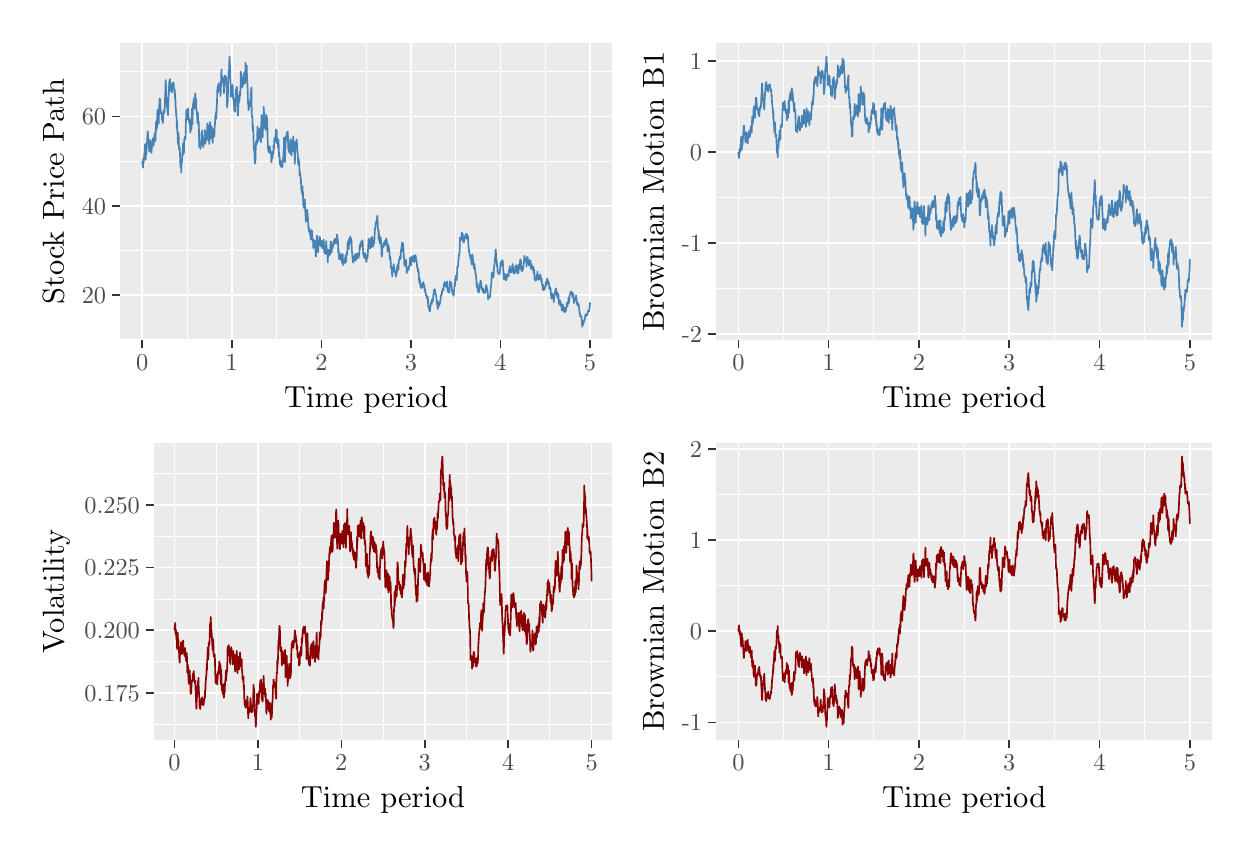
\begin{tikzpicture}[x=1pt,y=1pt]
\definecolor{fillColor}{RGB}{255,255,255}
\path[use as bounding box,fill=fillColor,fill opacity=0.00] (0,0) rectangle (433.62,289.08);
\begin{scope}
\path[clip] (  0.00,144.54) rectangle (216.81,289.08);
\definecolor{drawColor}{RGB}{255,255,255}
\definecolor{fillColor}{RGB}{255,255,255}

\path[draw=drawColor,line width= 0.6pt,line join=round,line cap=round,fill=fillColor] (  0.00,144.54) rectangle (216.81,289.08);
\end{scope}
\begin{scope}
\path[clip] ( 33.30,176.07) rectangle (211.31,283.58);
\definecolor{fillColor}{gray}{0.92}

\path[fill=fillColor] ( 33.30,176.07) rectangle (211.31,283.58);
\definecolor{drawColor}{RGB}{255,255,255}

\path[draw=drawColor,line width= 0.3pt,line join=round] ( 33.30,176.28) --
	(211.31,176.28);

\path[draw=drawColor,line width= 0.3pt,line join=round] ( 33.30,208.57) --
	(211.31,208.57);

\path[draw=drawColor,line width= 0.3pt,line join=round] ( 33.30,240.86) --
	(211.31,240.86);

\path[draw=drawColor,line width= 0.3pt,line join=round] ( 33.30,273.15) --
	(211.31,273.15);

\path[draw=drawColor,line width= 0.3pt,line join=round] ( 57.57,176.07) --
	( 57.57,283.58);

\path[draw=drawColor,line width= 0.3pt,line join=round] ( 89.94,176.07) --
	( 89.94,283.58);

\path[draw=drawColor,line width= 0.3pt,line join=round] (122.30,176.07) --
	(122.30,283.58);

\path[draw=drawColor,line width= 0.3pt,line join=round] (154.67,176.07) --
	(154.67,283.58);

\path[draw=drawColor,line width= 0.3pt,line join=round] (187.04,176.07) --
	(187.04,283.58);

\path[draw=drawColor,line width= 0.6pt,line join=round] ( 33.30,192.43) --
	(211.31,192.43);

\path[draw=drawColor,line width= 0.6pt,line join=round] ( 33.30,224.71) --
	(211.31,224.71);

\path[draw=drawColor,line width= 0.6pt,line join=round] ( 33.30,257.00) --
	(211.31,257.00);

\path[draw=drawColor,line width= 0.6pt,line join=round] ( 41.39,176.07) --
	( 41.39,283.58);

\path[draw=drawColor,line width= 0.6pt,line join=round] ( 73.75,176.07) --
	( 73.75,283.58);

\path[draw=drawColor,line width= 0.6pt,line join=round] (106.12,176.07) --
	(106.12,283.58);

\path[draw=drawColor,line width= 0.6pt,line join=round] (138.49,176.07) --
	(138.49,283.58);

\path[draw=drawColor,line width= 0.6pt,line join=round] (170.85,176.07) --
	(170.85,283.58);

\path[draw=drawColor,line width= 0.6pt,line join=round] (203.22,176.07) --
	(203.22,283.58);
\definecolor{drawColor}{RGB}{70,130,180}

\path[draw=drawColor,line width= 0.6pt,line join=round] ( 41.39,240.86) --
	( 41.48,239.67) --
	( 41.56,240.02) --
	( 41.65,238.45) --
	( 41.74,241.40) --
	( 41.83,242.02) --
	( 41.92,240.46) --
	( 42.01,241.37) --
	( 42.10,242.78) --
	( 42.19,243.88) --
	( 42.27,243.29) --
	( 42.36,246.21) --
	( 42.45,246.98) --
	( 42.54,245.74) --
	( 42.63,241.37) --
	( 42.72,243.51) --
	( 42.81,243.42) --
	( 42.89,243.39) --
	( 42.98,245.21) --
	( 43.07,246.82) --
	( 43.16,248.01) --
	( 43.25,249.85) --
	( 43.34,251.45) --
	( 43.43,251.60) --
	( 43.52,247.48) --
	( 43.60,248.73) --
	( 43.69,248.61) --
	( 43.78,248.30) --
	( 43.87,245.33) --
	( 43.96,244.39) --
	( 44.05,245.21) --
	( 44.14,247.87) --
	( 44.22,247.67) --
	( 44.31,248.45) --
	( 44.40,248.34) --
	( 44.49,245.56) --
	( 44.58,244.74) --
	( 44.67,243.97) --
	( 44.76,243.86) --
	( 44.85,245.99) --
	( 44.93,247.50) --
	( 45.02,247.17) --
	( 45.11,246.66) --
	( 45.20,248.05) --
	( 45.29,249.17) --
	( 45.38,247.77) --
	( 45.47,246.35) --
	( 45.56,247.07) --
	( 45.64,248.61) --
	( 45.73,248.38) --
	( 45.82,250.16) --
	( 45.91,250.97) --
	( 46.00,249.71) --
	( 46.09,250.41) --
	( 46.18,248.09) --
	( 46.26,250.97) --
	( 46.35,255.05) --
	( 46.44,254.27) --
	( 46.53,252.06) --
	( 46.62,253.25) --
	( 46.71,252.96) --
	( 46.80,257.99) --
	( 46.89,257.90) --
	( 46.97,259.40) --
	( 47.06,259.46) --
	( 47.15,257.83) --
	( 47.24,258.24) --
	( 47.33,254.31) --
	( 47.42,257.41) --
	( 47.51,257.74) --
	( 47.59,262.45) --
	( 47.68,263.52) --
	( 47.77,261.91) --
	( 47.86,263.28) --
	( 47.95,261.17) --
	( 48.04,258.38) --
	( 48.13,259.02) --
	( 48.22,258.05) --
	( 48.30,258.05) --
	( 48.39,258.21) --
	( 48.48,256.93) --
	( 48.57,255.70) --
	( 48.66,255.41) --
	( 48.75,257.92) --
	( 48.84,254.61) --
	( 48.92,255.87) --
	( 49.01,256.58) --
	( 49.10,258.87) --
	( 49.19,258.21) --
	( 49.28,259.01) --
	( 49.37,259.60) --
	( 49.46,258.40) --
	( 49.55,261.04) --
	( 49.63,263.62) --
	( 49.72,265.21) --
	( 49.81,268.84) --
	( 49.90,270.15) --
	( 49.99,267.13) --
	( 50.08,265.80) --
	( 50.17,262.98) --
	( 50.25,261.92) --
	( 50.34,260.53) --
	( 50.43,260.62) --
	( 50.52,258.60) --
	( 50.61,258.95) --
	( 50.70,257.51) --
	( 50.79,261.34) --
	( 50.88,262.94) --
	( 50.96,265.00) --
	( 51.05,265.87) --
	( 51.14,269.74) --
	( 51.23,268.24) --
	( 51.32,267.16) --
	( 51.41,270.49) --
	( 51.50,268.95) --
	( 51.58,268.46) --
	( 51.67,267.54) --
	( 51.76,266.79) --
	( 51.85,266.15) --
	( 51.94,267.29) --
	( 52.03,266.88) --
	( 52.12,265.70) --
	( 52.21,268.79) --
	( 52.29,268.29) --
	( 52.38,267.87) --
	( 52.47,267.63) --
	( 52.56,269.30) --
	( 52.65,269.12) --
	( 52.74,269.03) --
	( 52.83,267.43) --
	( 52.92,266.67) --
	( 53.00,266.81) --
	( 53.09,265.45) --
	( 53.18,266.67) --
	( 53.27,263.15) --
	( 53.36,263.84) --
	( 53.45,260.35) --
	( 53.54,259.68) --
	( 53.62,258.52) --
	( 53.71,257.09) --
	( 53.80,256.96) --
	( 53.89,252.82) --
	( 53.98,255.29) --
	( 54.07,251.73) --
	( 54.16,250.77) --
	( 54.25,248.47) --
	( 54.33,246.95) --
	( 54.42,251.12) --
	( 54.51,251.15) --
	( 54.60,248.49) --
	( 54.69,245.17) --
	( 54.78,246.06) --
	( 54.87,246.02) --
	( 54.95,245.39) --
	( 55.04,243.56) --
	( 55.13,240.68) --
	( 55.22,238.65) --
	( 55.31,240.50) --
	( 55.40,239.33) --
	( 55.49,236.75) --
	( 55.58,240.15) --
	( 55.66,240.95) --
	( 55.75,240.49) --
	( 55.84,242.49) --
	( 55.93,244.19) --
	( 56.02,242.98) --
	( 56.11,247.23) --
	( 56.20,246.72) --
	( 56.28,243.89) --
	( 56.37,243.61) --
	( 56.46,244.01) --
	( 56.55,248.49) --
	( 56.64,248.71) --
	( 56.73,249.63) --
	( 56.82,249.47) --
	( 56.91,248.79) --
	( 56.99,248.72) --
	( 57.08,250.32) --
	( 57.17,254.57) --
	( 57.26,256.75) --
	( 57.35,259.35) --
	( 57.44,256.65) --
	( 57.53,258.77) --
	( 57.61,259.25) --
	( 57.70,256.03) --
	( 57.79,257.14) --
	( 57.88,256.80) --
	( 57.97,259.96) --
	( 58.06,258.27) --
	( 58.15,257.33) --
	( 58.24,255.32) --
	( 58.32,254.95) --
	( 58.41,255.80) --
	( 58.50,254.24) --
	( 58.59,255.99) --
	( 58.68,253.40) --
	( 58.77,251.20) --
	( 58.86,254.18) --
	( 58.94,252.03) --
	( 59.03,252.88) --
	( 59.12,252.09) --
	( 59.21,252.94) --
	( 59.30,256.47) --
	( 59.39,259.89) --
	( 59.48,259.16) --
	( 59.57,254.14) --
	( 59.65,259.42) --
	( 59.74,260.88) --
	( 59.83,262.09) --
	( 59.92,262.06) --
	( 60.01,263.20) --
	( 60.10,262.83) --
	( 60.19,263.77) --
	( 60.28,262.87) --
	( 60.36,259.78) --
	( 60.45,261.96) --
	( 60.54,265.36) --
	( 60.63,264.65) --
	( 60.72,261.79) --
	( 60.81,263.23) --
	( 60.90,263.13) --
	( 60.98,259.22) --
	( 61.07,259.22) --
	( 61.16,257.84) --
	( 61.25,257.10) --
	( 61.34,254.60) --
	( 61.43,258.42) --
	( 61.52,257.70) --
	( 61.61,254.21) --
	( 61.69,254.63) --
	( 61.78,255.19) --
	( 61.87,253.09) --
	( 61.96,247.03) --
	( 62.05,245.76) --
	( 62.14,246.88) --
	( 62.23,246.76) --
	( 62.31,246.57) --
	( 62.40,247.68) --
	( 62.49,245.30) --
	( 62.58,247.46) --
	( 62.67,247.45) --
	( 62.76,248.86) --
	( 62.85,250.95) --
	( 62.94,251.42) --
	( 63.02,249.60) --
	( 63.11,251.97) --
	( 63.20,247.82) --
	( 63.29,246.72) --
	( 63.38,246.21) --
	( 63.47,245.89) --
	( 63.56,247.90) --
	( 63.64,248.17) --
	( 63.73,248.99) --
	( 63.82,248.85) --
	( 63.91,248.35) --
	( 64.00,249.75) --
	( 64.09,252.09) --
	( 64.18,247.10) --
	( 64.27,248.24) --
	( 64.35,248.99) --
	( 64.44,248.13) --
	( 64.53,250.04) --
	( 64.62,249.25) --
	( 64.71,248.67) --
	( 64.80,250.40) --
	( 64.89,253.93) --
	( 64.97,254.49) --
	( 65.06,253.60) --
	( 65.15,251.10) --
	( 65.24,250.42) --
	( 65.33,248.49) --
	( 65.42,247.97) --
	( 65.51,248.76) --
	( 65.60,247.04) --
	( 65.68,252.32) --
	( 65.77,252.64) --
	( 65.86,255.00) --
	( 65.95,250.14) --
	( 66.04,251.65) --
	( 66.13,248.93) --
	( 66.22,250.79) --
	( 66.30,251.61) --
	( 66.39,250.77) --
	( 66.48,253.49) --
	( 66.57,252.02) --
	( 66.66,250.81) --
	( 66.75,248.75) --
	( 66.84,247.41) --
	( 66.93,249.29) --
	( 67.01,250.17) --
	( 67.10,252.23) --
	( 67.19,251.42) --
	( 67.28,252.19) --
	( 67.37,252.70) --
	( 67.46,249.73) --
	( 67.55,253.35) --
	( 67.64,253.63) --
	( 67.72,255.24) --
	( 67.81,257.27) --
	( 67.90,257.16) --
	( 67.99,256.50) --
	( 68.08,258.42) --
	( 68.17,256.14) --
	( 68.26,260.36) --
	( 68.34,259.51) --
	( 68.43,263.14) --
	( 68.52,266.55) --
	( 68.61,266.74) --
	( 68.70,268.05) --
	( 68.79,265.66) --
	( 68.88,266.40) --
	( 68.97,268.81) --
	( 69.05,269.04) --
	( 69.14,267.97) --
	( 69.23,266.45) --
	( 69.32,266.36) --
	( 69.41,268.83) --
	( 69.50,267.69) --
	( 69.59,267.41) --
	( 69.67,264.41) --
	( 69.76,265.53) --
	( 69.85,268.53) --
	( 69.94,272.03) --
	( 70.03,273.98) --
	( 70.12,269.46) --
	( 70.21,270.59) --
	( 70.30,271.67) --
	( 70.38,270.83) --
	( 70.47,271.23) --
	( 70.56,269.17) --
	( 70.65,270.77) --
	( 70.74,269.99) --
	( 70.83,266.29) --
	( 70.92,265.44) --
	( 71.00,268.57) --
	( 71.09,267.79) --
	( 71.18,269.49) --
	( 71.27,271.72) --
	( 71.36,271.73) --
	( 71.45,270.89) --
	( 71.54,269.63) --
	( 71.63,271.38) --
	( 71.71,268.84) --
	( 71.80,269.42) --
	( 71.89,268.74) --
	( 71.98,263.42) --
	( 72.07,260.24) --
	( 72.16,262.26) --
	( 72.25,261.83) --
	( 72.33,263.63) --
	( 72.42,267.91) --
	( 72.51,271.34) --
	( 72.60,272.96) --
	( 72.69,273.87) --
	( 72.78,273.41) --
	( 72.87,277.22) --
	( 72.96,278.69) --
	( 73.04,275.77) --
	( 73.13,275.39) --
	( 73.22,270.69) --
	( 73.31,270.23) --
	( 73.40,264.09) --
	( 73.49,267.07) --
	( 73.58,265.60) --
	( 73.66,264.61) --
	( 73.75,264.23) --
	( 73.84,265.62) --
	( 73.93,267.18) --
	( 74.02,268.50) --
	( 74.11,267.16) --
	( 74.20,263.99) --
	( 74.29,263.11) --
	( 74.37,263.73) --
	( 74.46,261.87) --
	( 74.55,261.71) --
	( 74.64,259.10) --
	( 74.73,259.08) --
	( 74.82,259.36) --
	( 74.91,259.04) --
	( 75.00,258.68) --
	( 75.08,262.55) --
	( 75.17,264.26) --
	( 75.26,266.80) --
	( 75.35,264.66) --
	( 75.44,265.03) --
	( 75.53,267.68) --
	( 75.62,267.54) --
	( 75.70,262.58) --
	( 75.79,263.36) --
	( 75.88,259.04) --
	( 75.97,257.26) --
	( 76.06,260.13) --
	( 76.15,261.50) --
	( 76.24,263.94) --
	( 76.33,264.63) --
	( 76.41,264.38) --
	( 76.50,262.27) --
	( 76.59,265.85) --
	( 76.68,265.96) --
	( 76.77,264.31) --
	( 76.86,266.28) --
	( 76.95,268.77) --
	( 77.03,273.22) --
	( 77.12,271.76) --
	( 77.21,270.83) --
	( 77.30,269.83) --
	( 77.39,268.95) --
	( 77.48,268.08) --
	( 77.57,267.39) --
	( 77.66,270.75) --
	( 77.74,269.09) --
	( 77.83,268.17) --
	( 77.92,269.70) --
	( 78.01,272.36) --
	( 78.10,270.51) --
	( 78.19,269.30) --
	( 78.28,270.53) --
	( 78.36,272.95) --
	( 78.45,272.35) --
	( 78.54,268.91) --
	( 78.63,272.93) --
	( 78.72,276.40) --
	( 78.81,274.64) --
	( 78.90,274.49) --
	( 78.99,270.19) --
	( 79.07,271.55) --
	( 79.16,275.41) --
	( 79.25,271.39) --
	( 79.34,269.53) --
	( 79.43,268.01) --
	( 79.52,266.42) --
	( 79.61,261.70) --
	( 79.69,262.83) --
	( 79.78,259.37) --
	( 79.87,259.31) --
	( 79.96,260.62) --
	( 80.05,260.18) --
	( 80.14,262.16) --
	( 80.23,262.10) --
	( 80.32,260.64) --
	( 80.40,262.08) --
	( 80.49,261.10) --
	( 80.58,265.06) --
	( 80.67,265.02) --
	( 80.76,266.98) --
	( 80.85,267.46) --
	( 80.94,260.44) --
	( 81.02,257.40) --
	( 81.11,256.48) --
	( 81.20,256.99) --
	( 81.29,251.91) --
	( 81.38,253.92) --
	( 81.47,252.64) --
	( 81.56,251.06) --
	( 81.65,247.84) --
	( 81.73,244.91) --
	( 81.82,245.02) --
	( 81.91,246.02) --
	( 82.00,241.86) --
	( 82.09,239.95) --
	( 82.18,240.95) --
	( 82.27,240.09) --
	( 82.36,244.16) --
	( 82.44,246.59) --
	( 82.53,247.78) --
	( 82.62,247.79) --
	( 82.71,248.35) --
	( 82.80,246.92) --
	( 82.89,248.17) --
	( 82.98,251.16) --
	( 83.06,253.40) --
	( 83.15,251.69) --
	( 83.24,248.33) --
	( 83.33,248.11) --
	( 83.42,249.00) --
	( 83.51,251.74) --
	( 83.60,249.00) --
	( 83.69,249.74) --
	( 83.77,250.22) --
	( 83.86,252.67) --
	( 83.95,252.61) --
	( 84.04,251.86) --
	( 84.13,249.48) --
	( 84.22,248.42) --
	( 84.31,247.69) --
	( 84.39,252.41) --
	( 84.48,257.52) --
	( 84.57,257.16) --
	( 84.66,254.90) --
	( 84.75,250.70) --
	( 84.84,251.76) --
	( 84.93,249.50) --
	( 85.02,254.15) --
	( 85.10,252.28) --
	( 85.19,252.51) --
	( 85.28,260.47) --
	( 85.37,258.01) --
	( 85.46,258.68) --
	( 85.55,256.26) --
	( 85.64,257.01) --
	( 85.72,255.12) --
	( 85.81,255.29) --
	( 85.90,254.65) --
	( 85.99,252.14) --
	( 86.08,252.17) --
	( 86.17,254.23) --
	( 86.26,257.60) --
	( 86.35,254.62) --
	( 86.43,254.09) --
	( 86.52,256.54) --
	( 86.61,254.14) --
	( 86.70,248.80) --
	( 86.79,246.91) --
	( 86.88,244.98) --
	( 86.97,245.07) --
	( 87.05,244.28) --
	( 87.14,244.73) --
	( 87.23,243.91) --
	( 87.32,244.63) --
	( 87.41,243.92) --
	( 87.50,246.23) --
	( 87.59,244.77) --
	( 87.68,245.34) --
	( 87.76,243.60) --
	( 87.85,244.00) --
	( 87.94,243.91) --
	( 88.03,240.64) --
	( 88.12,240.37) --
	( 88.21,242.59) --
	( 88.30,243.89) --
	( 88.38,244.17) --
	( 88.47,241.85) --
	( 88.56,244.08) --
	( 88.65,244.23) --
	( 88.74,243.35) --
	( 88.83,246.52) --
	( 88.92,244.99) --
	( 89.01,245.59) --
	( 89.09,248.11) --
	( 89.18,249.32) --
	( 89.27,248.70) --
	( 89.36,247.85) --
	( 89.45,248.56) --
	( 89.54,249.60) --
	( 89.63,249.64) --
	( 89.72,252.32) --
	( 89.80,252.19) --
	( 89.89,250.73) --
	( 89.98,251.83) --
	( 90.07,247.27) --
	( 90.16,248.05) --
	( 90.25,249.05) --
	( 90.34,248.60) --
	( 90.42,246.34) --
	( 90.51,245.56) --
	( 90.60,248.61) --
	( 90.69,247.11) --
	( 90.78,242.46) --
	( 90.87,244.01) --
	( 90.96,243.04) --
	( 91.05,242.06) --
	( 91.13,239.74) --
	( 91.22,239.70) --
	( 91.31,241.01) --
	( 91.40,239.90) --
	( 91.49,238.77) --
	( 91.58,240.79) --
	( 91.67,240.33) --
	( 91.75,240.03) --
	( 91.84,238.86) --
	( 91.93,240.52) --
	( 92.02,238.65) --
	( 92.11,240.22) --
	( 92.20,241.73) --
	( 92.29,240.84) --
	( 92.38,242.44) --
	( 92.46,244.33) --
	( 92.55,245.44) --
	( 92.64,249.42) --
	( 92.73,245.44) --
	( 92.82,243.15) --
	( 92.91,240.51) --
	( 93.00,240.82) --
	( 93.08,243.80) --
	( 93.17,247.04) --
	( 93.26,248.02) --
	( 93.35,249.78) --
	( 93.44,249.48) --
	( 93.53,250.43) --
	( 93.62,251.20) --
	( 93.71,249.64) --
	( 93.79,249.04) --
	( 93.88,248.77) --
	( 93.97,251.58) --
	( 94.06,249.44) --
	( 94.15,245.15) --
	( 94.24,246.65) --
	( 94.33,245.04) --
	( 94.41,244.19) --
	( 94.50,245.94) --
	( 94.59,244.44) --
	( 94.68,243.77) --
	( 94.77,246.68) --
	( 94.86,247.72) --
	( 94.95,248.81) --
	( 95.04,248.53) --
	( 95.12,246.24) --
	( 95.21,243.29) --
	( 95.30,242.86) --
	( 95.39,246.70) --
	( 95.48,247.13) --
	( 95.57,247.46) --
	( 95.66,248.12) --
	( 95.74,247.35) --
	( 95.83,244.57) --
	( 95.92,249.77) --
	( 96.01,248.91) --
	( 96.10,248.31) --
	( 96.19,244.71) --
	( 96.28,244.23) --
	( 96.37,243.75) --
	( 96.45,243.25) --
	( 96.54,239.82) --
	( 96.63,243.14) --
	( 96.72,246.53) --
	( 96.81,247.89) --
	( 96.90,245.69) --
	( 96.99,247.09) --
	( 97.08,246.60) --
	( 97.16,245.97) --
	( 97.25,248.65) --
	( 97.34,246.18) --
	( 97.43,245.17) --
	( 97.52,243.74) --
	( 97.61,243.78) --
	( 97.70,240.75) --
	( 97.78,239.43) --
	( 97.87,240.76) --
	( 97.96,241.63) --
	( 98.05,239.79) --
	( 98.14,240.83) --
	( 98.23,236.26) --
	( 98.32,235.65) --
	( 98.41,236.92) --
	( 98.49,235.73) --
	( 98.58,235.67) --
	( 98.67,232.82) --
	( 98.76,234.29) --
	( 98.85,231.04) --
	( 98.94,230.48) --
	( 99.03,230.05) --
	( 99.11,230.16) --
	( 99.20,228.77) --
	( 99.29,231.80) --
	( 99.38,229.35) --
	( 99.47,229.78) --
	( 99.56,224.85) --
	( 99.65,224.85) --
	( 99.74,225.66) --
	( 99.82,223.93) --
	( 99.91,225.03) --
	(100.00,225.55) --
	(100.09,227.11) --
	(100.18,225.74) --
	(100.27,224.19) --
	(100.36,221.41) --
	(100.44,220.92) --
	(100.53,218.90) --
	(100.62,219.91) --
	(100.71,220.02) --
	(100.80,223.28) --
	(100.89,221.48) --
	(100.98,223.28) --
	(101.07,222.46) --
	(101.15,220.22) --
	(101.24,221.08) --
	(101.33,218.92) --
	(101.42,217.37) --
	(101.51,216.32) --
	(101.60,216.62) --
	(101.69,215.20) --
	(101.77,216.70) --
	(101.86,214.99) --
	(101.95,215.29) --
	(102.04,215.49) --
	(102.13,214.00) --
	(102.22,213.42) --
	(102.31,212.53) --
	(102.40,213.81) --
	(102.48,215.93) --
	(102.57,214.47) --
	(102.66,215.75) --
	(102.75,215.65) --
	(102.84,212.89) --
	(102.93,211.88) --
	(103.02,212.49) --
	(103.10,212.68) --
	(103.19,209.42) --
	(103.28,210.15) --
	(103.37,211.00) --
	(103.46,210.60) --
	(103.55,209.68) --
	(103.64,212.20) --
	(103.73,212.08) --
	(103.81,212.06) --
	(103.90,210.57) --
	(103.99,208.84) --
	(104.08,206.92) --
	(104.17,206.41) --
	(104.26,208.05) --
	(104.35,210.22) --
	(104.43,212.24) --
	(104.52,213.96) --
	(104.61,213.63) --
	(104.70,211.98) --
	(104.79,211.55) --
	(104.88,208.39) --
	(104.97,208.00) --
	(105.06,210.05) --
	(105.14,210.22) --
	(105.23,211.62) --
	(105.32,212.26) --
	(105.41,211.23) --
	(105.50,213.50) --
	(105.59,213.39) --
	(105.68,212.08) --
	(105.77,212.18) --
	(105.85,210.17) --
	(105.94,211.28) --
	(106.03,211.93) --
	(106.12,211.46) --
	(106.21,210.83) --
	(106.30,212.04) --
	(106.39,210.64) --
	(106.47,209.37) --
	(106.56,209.91) --
	(106.65,209.33) --
	(106.74,210.50) --
	(106.83,210.24) --
	(106.92,211.77) --
	(107.01,212.42) --
	(107.10,209.45) --
	(107.18,207.77) --
	(107.27,209.34) --
	(107.36,210.21) --
	(107.45,208.98) --
	(107.54,207.29) --
	(107.63,208.55) --
	(107.72,207.54) --
	(107.80,209.74) --
	(107.89,211.98) --
	(107.98,210.08) --
	(108.07,209.01) --
	(108.16,207.44) --
	(108.25,208.26) --
	(108.34,206.66) --
	(108.43,204.22) --
	(108.51,206.54) --
	(108.60,207.75) --
	(108.69,208.75) --
	(108.78,207.92) --
	(108.87,207.91) --
	(108.96,208.67) --
	(109.05,207.08) --
	(109.13,206.93) --
	(109.22,207.14) --
	(109.31,209.19) --
	(109.40,209.99) --
	(109.49,211.61) --
	(109.58,211.79) --
	(109.67,210.34) --
	(109.76,209.91) --
	(109.84,207.81) --
	(109.93,208.94) --
	(110.02,210.70) --
	(110.11,210.62) --
	(110.20,209.37) --
	(110.29,210.73) --
	(110.38,210.91) --
	(110.46,210.42) --
	(110.55,211.84) --
	(110.64,210.86) --
	(110.73,212.33) --
	(110.82,211.23) --
	(110.91,211.73) --
	(111.00,212.88) --
	(111.09,211.12) --
	(111.17,211.63) --
	(111.26,211.49) --
	(111.35,212.36) --
	(111.44,211.33) --
	(111.53,211.22) --
	(111.62,213.00) --
	(111.71,213.22) --
	(111.79,214.31) --
	(111.88,214.01) --
	(111.97,212.63) --
	(112.06,212.62) --
	(112.15,211.01) --
	(112.24,207.69) --
	(112.33,209.11) --
	(112.42,207.76) --
	(112.50,205.54) --
	(112.59,206.70) --
	(112.68,206.69) --
	(112.77,205.98) --
	(112.86,205.77) --
	(112.95,205.27) --
	(113.04,206.43) --
	(113.13,207.29) --
	(113.21,205.21) --
	(113.30,205.62) --
	(113.39,206.47) --
	(113.48,207.26) --
	(113.57,204.35) --
	(113.66,204.08) --
	(113.75,206.33) --
	(113.83,207.27) --
	(113.92,205.22) --
	(114.01,203.29) --
	(114.10,203.84) --
	(114.19,203.65) --
	(114.28,204.73) --
	(114.37,205.07) --
	(114.46,205.16) --
	(114.54,205.37) --
	(114.63,205.56) --
	(114.72,204.09) --
	(114.81,206.75) --
	(114.90,205.07) --
	(114.99,205.05) --
	(115.08,204.43) --
	(115.16,206.48) --
	(115.25,207.67) --
	(115.34,206.99) --
	(115.43,207.24) --
	(115.52,208.63) --
	(115.61,211.36) --
	(115.70,211.75) --
	(115.79,210.41) --
	(115.87,209.18) --
	(115.96,211.65) --
	(116.05,209.00) --
	(116.14,212.75) --
	(116.23,212.41) --
	(116.32,211.82) --
	(116.41,212.02) --
	(116.49,213.22) --
	(116.58,213.62) --
	(116.67,211.05) --
	(116.76,211.49) --
	(116.85,212.07) --
	(116.94,212.92) --
	(117.03,211.57) --
	(117.12,208.55) --
	(117.20,208.15) --
	(117.29,207.01) --
	(117.38,206.10) --
	(117.47,204.99) --
	(117.56,204.54) --
	(117.65,204.18) --
	(117.74,205.08) --
	(117.82,206.21) --
	(117.91,205.28) --
	(118.00,204.93) --
	(118.09,205.34) --
	(118.18,206.95) --
	(118.27,206.88) --
	(118.36,204.88) --
	(118.45,205.14) --
	(118.53,205.01) --
	(118.62,207.03) --
	(118.71,207.44) --
	(118.80,206.70) --
	(118.89,206.18) --
	(118.98,205.59) --
	(119.07,205.80) --
	(119.15,206.01) --
	(119.24,207.07) --
	(119.33,207.45) --
	(119.42,207.01) --
	(119.51,205.90) --
	(119.60,206.64) --
	(119.69,206.57) --
	(119.78,206.78) --
	(119.86,208.08) --
	(119.95,210.18) --
	(120.04,209.00) --
	(120.13,211.00) --
	(120.22,209.91) --
	(120.31,210.24) --
	(120.40,210.52) --
	(120.49,210.17) --
	(120.57,211.90) --
	(120.66,211.06) --
	(120.75,211.89) --
	(120.84,211.88) --
	(120.93,210.69) --
	(121.02,212.21) --
	(121.11,209.54) --
	(121.19,208.89) --
	(121.28,207.02) --
	(121.37,207.25) --
	(121.46,207.56) --
	(121.55,206.23) --
	(121.64,206.99) --
	(121.73,205.77) --
	(121.82,206.53) --
	(121.90,206.81) --
	(121.99,207.65) --
	(122.08,206.53) --
	(122.17,206.65) --
	(122.26,206.10) --
	(122.35,204.40) --
	(122.44,204.58) --
	(122.52,206.58) --
	(122.61,205.82) --
	(122.70,205.59) --
	(122.79,206.38) --
	(122.88,206.42) --
	(122.97,208.68) --
	(123.06,209.57) --
	(123.15,212.41) --
	(123.23,212.86) --
	(123.32,211.40) --
	(123.41,211.93) --
	(123.50,210.76) --
	(123.59,209.50) --
	(123.68,209.27) --
	(123.77,210.41) --
	(123.85,210.84) --
	(123.94,211.85) --
	(124.03,213.01) --
	(124.12,212.79) --
	(124.21,209.71) --
	(124.30,210.68) --
	(124.39,213.37) --
	(124.48,213.45) --
	(124.56,211.70) --
	(124.65,211.23) --
	(124.74,210.06) --
	(124.83,210.01) --
	(124.92,210.84) --
	(125.01,211.92) --
	(125.10,212.22) --
	(125.18,211.03) --
	(125.27,212.05) --
	(125.36,213.75) --
	(125.45,216.68) --
	(125.54,216.01) --
	(125.63,216.65) --
	(125.72,218.26) --
	(125.81,218.10) --
	(125.89,218.82) --
	(125.98,219.12) --
	(126.07,218.93) --
	(126.16,219.17) --
	(126.25,220.51) --
	(126.34,221.09) --
	(126.43,220.43) --
	(126.51,217.25) --
	(126.60,216.17) --
	(126.69,216.14) --
	(126.78,212.77) --
	(126.87,215.59) --
	(126.96,213.62) --
	(127.05,212.11) --
	(127.14,213.96) --
	(127.22,211.11) --
	(127.31,212.03) --
	(127.40,211.60) --
	(127.49,212.17) --
	(127.58,213.28) --
	(127.67,212.05) --
	(127.76,211.16) --
	(127.85,207.43) --
	(127.93,206.30) --
	(128.02,206.74) --
	(128.11,207.32) --
	(128.20,209.70) --
	(128.29,209.78) --
	(128.38,210.34) --
	(128.47,210.43) --
	(128.55,209.83) --
	(128.64,210.75) --
	(128.73,211.32) --
	(128.82,211.48) --
	(128.91,210.46) --
	(129.00,210.41) --
	(129.09,211.37) --
	(129.18,212.22) --
	(129.26,211.61) --
	(129.35,210.77) --
	(129.44,211.40) --
	(129.53,212.71) --
	(129.62,212.87) --
	(129.71,212.47) --
	(129.80,211.35) --
	(129.88,210.83) --
	(129.97,209.00) --
	(130.06,208.16) --
	(130.15,209.50) --
	(130.24,210.85) --
	(130.33,209.77) --
	(130.42,210.03) --
	(130.51,210.11) --
	(130.59,208.08) --
	(130.68,209.04) --
	(130.77,206.75) --
	(130.86,205.30) --
	(130.95,206.43) --
	(131.04,205.81) --
	(131.13,205.56) --
	(131.21,203.73) --
	(131.30,202.13) --
	(131.39,202.51) --
	(131.48,202.32) --
	(131.57,201.69) --
	(131.66,200.28) --
	(131.75,199.15) --
	(131.84,201.20) --
	(131.92,200.86) --
	(132.01,201.66) --
	(132.10,202.49) --
	(132.19,203.30) --
	(132.28,203.62) --
	(132.37,202.26) --
	(132.46,201.18) --
	(132.54,201.97) --
	(132.63,200.58) --
	(132.72,201.12) --
	(132.81,200.57) --
	(132.90,200.16) --
	(132.99,199.35) --
	(133.08,199.12) --
	(133.17,200.00) --
	(133.25,200.46) --
	(133.34,200.22) --
	(133.43,201.11) --
	(133.52,202.83) --
	(133.61,202.83) --
	(133.70,203.33) --
	(133.79,203.63) --
	(133.87,202.57) --
	(133.96,201.58) --
	(134.05,203.59) --
	(134.14,204.55) --
	(134.23,205.37) --
	(134.32,205.54) --
	(134.41,206.08) --
	(134.50,206.25) --
	(134.58,206.30) --
	(134.67,206.56) --
	(134.76,205.40) --
	(134.85,208.10) --
	(134.94,209.04) --
	(135.03,208.74) --
	(135.12,210.18) --
	(135.21,209.41) --
	(135.29,211.46) --
	(135.38,210.98) --
	(135.47,208.13) --
	(135.56,209.73) --
	(135.65,211.09) --
	(135.74,210.14) --
	(135.83,208.43) --
	(135.91,206.27) --
	(136.00,205.97) --
	(136.09,203.90) --
	(136.18,203.01) --
	(136.27,203.18) --
	(136.36,204.10) --
	(136.45,203.21) --
	(136.54,203.07) --
	(136.62,203.35) --
	(136.71,205.20) --
	(136.80,204.13) --
	(136.89,202.38) --
	(136.98,200.42) --
	(137.07,200.99) --
	(137.16,200.93) --
	(137.24,201.72) --
	(137.33,201.58) --
	(137.42,201.99) --
	(137.51,202.22) --
	(137.60,202.25) --
	(137.69,201.59) --
	(137.78,202.91) --
	(137.87,202.47) --
	(137.95,203.18) --
	(138.04,203.35) --
	(138.13,205.27) --
	(138.22,206.06) --
	(138.31,205.68) --
	(138.40,205.67) --
	(138.49,205.53) --
	(138.57,203.20) --
	(138.66,205.02) --
	(138.75,206.19) --
	(138.84,205.33) --
	(138.93,205.75) --
	(139.02,206.02) --
	(139.11,204.75) --
	(139.20,206.39) --
	(139.28,206.11) --
	(139.37,206.32) --
	(139.46,206.77) --
	(139.55,205.64) --
	(139.64,204.43) --
	(139.73,204.37) --
	(139.82,205.00) --
	(139.90,205.09) --
	(139.99,205.87) --
	(140.08,206.24) --
	(140.17,206.86) --
	(140.26,205.26) --
	(140.35,206.01) --
	(140.44,205.12) --
	(140.53,204.61) --
	(140.61,204.49) --
	(140.70,202.69) --
	(140.79,202.58) --
	(140.88,202.12) --
	(140.97,201.36) --
	(141.06,200.79) --
	(141.15,202.06) --
	(141.23,200.75) --
	(141.32,200.53) --
	(141.41,198.01) --
	(141.50,197.36) --
	(141.59,196.88) --
	(141.68,198.34) --
	(141.77,197.40) --
	(141.86,196.57) --
	(141.94,195.26) --
	(142.03,195.43) --
	(142.12,196.48) --
	(142.21,195.36) --
	(142.30,194.97) --
	(142.39,196.21) --
	(142.48,195.57) --
	(142.57,196.20) --
	(142.65,196.56) --
	(142.74,195.34) --
	(142.83,196.45) --
	(142.92,197.19) --
	(143.01,196.73) --
	(143.10,195.88) --
	(143.19,195.52) --
	(143.27,196.26) --
	(143.36,195.74) --
	(143.45,194.02) --
	(143.54,193.90) --
	(143.63,194.57) --
	(143.72,193.54) --
	(143.81,193.33) --
	(143.90,192.28) --
	(143.98,192.37) --
	(144.07,192.26) --
	(144.16,192.23) --
	(144.25,191.71) --
	(144.34,191.12) --
	(144.43,191.83) --
	(144.52,191.92) --
	(144.60,191.77) --
	(144.69,189.09) --
	(144.78,188.11) --
	(144.87,188.68) --
	(144.96,188.37) --
	(145.05,187.45) --
	(145.14,187.13) --
	(145.23,186.86) --
	(145.31,186.49) --
	(145.40,186.85) --
	(145.49,187.95) --
	(145.58,188.69) --
	(145.67,189.64) --
	(145.76,189.38) --
	(145.85,190.04) --
	(145.93,189.26) --
	(146.02,189.15) --
	(146.11,190.84) --
	(146.20,190.83) --
	(146.29,190.58) --
	(146.38,190.11) --
	(146.47,190.73) --
	(146.56,192.42) --
	(146.64,192.77) --
	(146.73,192.55) --
	(146.82,194.29) --
	(146.91,193.61) --
	(147.00,194.59) --
	(147.09,194.21) --
	(147.18,193.32) --
	(147.26,194.36) --
	(147.35,192.78) --
	(147.44,192.52) --
	(147.53,192.54) --
	(147.62,192.16) --
	(147.71,190.80) --
	(147.80,190.28) --
	(147.89,189.05) --
	(147.97,190.52) --
	(148.06,189.04) --
	(148.15,187.43) --
	(148.24,187.94) --
	(148.33,188.61) --
	(148.42,188.46) --
	(148.51,188.31) --
	(148.59,188.85) --
	(148.68,189.91) --
	(148.77,188.67) --
	(148.86,189.66) --
	(148.95,189.81) --
	(149.04,189.54) --
	(149.13,190.52) --
	(149.22,191.27) --
	(149.30,192.31) --
	(149.39,192.06) --
	(149.48,192.71) --
	(149.57,192.95) --
	(149.66,192.52) --
	(149.75,193.99) --
	(149.84,194.13) --
	(149.93,194.08) --
	(150.01,194.54) --
	(150.10,194.88) --
	(150.19,194.26) --
	(150.28,194.21) --
	(150.37,196.48) --
	(150.46,196.41) --
	(150.55,196.14) --
	(150.63,196.80) --
	(150.72,197.17) --
	(150.81,196.67) --
	(150.90,195.68) --
	(150.99,196.44) --
	(151.08,196.55) --
	(151.17,196.99) --
	(151.26,196.72) --
	(151.34,195.21) --
	(151.43,195.27) --
	(151.52,197.39) --
	(151.61,196.03) --
	(151.70,195.14) --
	(151.79,193.96) --
	(151.88,193.65) --
	(151.96,194.83) --
	(152.05,194.69) --
	(152.14,194.47) --
	(152.23,193.35) --
	(152.32,193.40) --
	(152.41,194.28) --
	(152.50,196.24) --
	(152.59,197.43) --
	(152.67,196.62) --
	(152.76,196.16) --
	(152.85,196.71) --
	(152.94,196.70) --
	(153.03,196.96) --
	(153.12,195.75) --
	(153.21,195.37) --
	(153.29,194.55) --
	(153.38,193.74) --
	(153.47,193.12) --
	(153.56,192.77) --
	(153.65,192.77) --
	(153.74,193.30) --
	(153.83,192.87) --
	(153.92,192.15) --
	(154.00,193.48) --
	(154.09,194.32) --
	(154.18,194.92) --
	(154.27,196.42) --
	(154.36,195.53) --
	(154.45,197.35) --
	(154.54,198.48) --
	(154.62,198.77) --
	(154.71,199.37) --
	(154.80,199.43) --
	(154.89,199.32) --
	(154.98,197.81) --
	(155.07,198.50) --
	(155.16,200.52) --
	(155.25,202.58) --
	(155.33,202.75) --
	(155.42,202.64) --
	(155.51,202.82) --
	(155.60,204.00) --
	(155.69,205.54) --
	(155.78,205.98) --
	(155.87,207.19) --
	(155.95,207.16) --
	(156.04,207.71) --
	(156.13,209.03) --
	(156.22,213.16) --
	(156.31,213.09) --
	(156.40,212.29) --
	(156.49,212.82) --
	(156.58,212.33) --
	(156.66,213.09) --
	(156.75,213.50) --
	(156.84,215.09) --
	(156.93,213.90) --
	(157.02,212.44) --
	(157.11,214.31) --
	(157.20,214.58) --
	(157.29,213.45) --
	(157.37,212.15) --
	(157.46,211.50) --
	(157.55,212.19) --
	(157.64,211.56) --
	(157.73,213.14) --
	(157.82,213.44) --
	(157.91,213.67) --
	(157.99,213.65) --
	(158.08,213.29) --
	(158.17,213.09) --
	(158.26,214.48) --
	(158.35,212.84) --
	(158.44,214.14) --
	(158.53,213.72) --
	(158.62,214.61) --
	(158.70,214.54) --
	(158.79,212.88) --
	(158.88,213.30) --
	(158.97,212.53) --
	(159.06,213.87) --
	(159.15,212.87) --
	(159.24,210.72) --
	(159.32,209.73) --
	(159.41,209.07) --
	(159.50,208.14) --
	(159.59,207.87) --
	(159.68,207.21) --
	(159.77,206.76) --
	(159.86,207.11) --
	(159.95,205.83) --
	(160.03,206.65) --
	(160.12,206.65) --
	(160.21,206.61) --
	(160.30,204.39) --
	(160.39,204.07) --
	(160.48,203.49) --
	(160.57,204.37) --
	(160.65,205.83) --
	(160.74,207.15) --
	(160.83,205.93) --
	(160.92,205.07) --
	(161.01,204.98) --
	(161.10,203.85) --
	(161.19,202.18) --
	(161.28,202.98) --
	(161.36,203.05) --
	(161.45,203.68) --
	(161.54,202.43) --
	(161.63,202.09) --
	(161.72,200.91) --
	(161.81,200.09) --
	(161.90,200.31) --
	(161.98,199.52) --
	(162.07,198.56) --
	(162.16,197.33) --
	(162.25,196.01) --
	(162.34,195.24) --
	(162.43,196.74) --
	(162.52,196.14) --
	(162.61,195.15) --
	(162.69,193.92) --
	(162.78,193.79) --
	(162.87,193.46) --
	(162.96,193.67) --
	(163.05,193.43) --
	(163.14,194.16) --
	(163.23,194.77) --
	(163.31,195.69) --
	(163.40,195.91) --
	(163.49,196.90) --
	(163.58,196.83) --
	(163.67,197.67) --
	(163.76,197.53) --
	(163.85,196.90) --
	(163.94,195.79) --
	(164.02,195.16) --
	(164.11,194.51) --
	(164.20,195.01) --
	(164.29,194.96) --
	(164.38,194.41) --
	(164.47,193.64) --
	(164.56,194.92) --
	(164.65,194.71) --
	(164.73,193.63) --
	(164.82,193.27) --
	(164.91,193.35) --
	(165.00,194.04) --
	(165.09,193.97) --
	(165.18,194.07) --
	(165.27,193.18) --
	(165.35,193.85) --
	(165.44,193.93) --
	(165.53,194.56) --
	(165.62,195.89) --
	(165.71,196.05) --
	(165.80,195.79) --
	(165.89,195.12) --
	(165.98,194.61) --
	(166.06,193.83) --
	(166.15,194.14) --
	(166.24,192.89) --
	(166.33,191.45) --
	(166.42,190.91) --
	(166.51,191.77) --
	(166.60,191.87) --
	(166.68,191.47) --
	(166.77,192.00) --
	(166.86,191.72) --
	(166.95,191.63) --
	(167.04,191.68) --
	(167.13,192.56) --
	(167.22,193.62) --
	(167.31,194.69) --
	(167.39,195.53) --
	(167.48,195.82) --
	(167.57,197.48) --
	(167.66,199.35) --
	(167.75,200.61) --
	(167.84,200.39) --
	(167.93,199.39) --
	(168.01,199.57) --
	(168.10,199.04) --
	(168.19,199.30) --
	(168.28,198.78) --
	(168.37,199.64) --
	(168.46,201.73) --
	(168.55,202.68) --
	(168.64,203.43) --
	(168.72,203.47) --
	(168.81,205.70) --
	(168.90,205.61) --
	(168.99,207.07) --
	(169.08,208.78) --
	(169.17,208.95) --
	(169.26,205.32) --
	(169.34,204.98) --
	(169.43,205.46) --
	(169.52,204.08) --
	(169.61,202.75) --
	(169.70,203.66) --
	(169.79,200.80) --
	(169.88,201.03) --
	(169.97,200.77) --
	(170.05,200.13) --
	(170.14,200.19) --
	(170.23,200.24) --
	(170.32,200.48) --
	(170.41,200.60) --
	(170.50,200.08) --
	(170.59,200.33) --
	(170.67,201.66) --
	(170.76,202.32) --
	(170.85,203.81) --
	(170.94,203.53) --
	(171.03,204.13) --
	(171.12,204.65) --
	(171.21,203.87) --
	(171.30,203.04) --
	(171.38,204.93) --
	(171.47,204.06) --
	(171.56,205.04) --
	(171.65,204.76) --
	(171.74,203.62) --
	(171.83,202.05) --
	(171.92,200.86) --
	(172.01,198.96) --
	(172.09,198.13) --
	(172.18,199.03) --
	(172.27,198.49) --
	(172.36,200.10) --
	(172.45,199.93) --
	(172.54,199.04) --
	(172.63,198.77) --
	(172.71,198.22) --
	(172.80,197.81) --
	(172.89,197.87) --
	(172.98,197.94) --
	(173.07,198.64) --
	(173.16,199.14) --
	(173.25,199.87) --
	(173.34,199.99) --
	(173.42,199.22) --
	(173.51,199.65) --
	(173.60,200.04) --
	(173.69,199.65) --
	(173.78,199.28) --
	(173.87,200.31) --
	(173.96,201.60) --
	(174.04,201.71) --
	(174.13,201.33) --
	(174.22,202.94) --
	(174.31,201.69) --
	(174.40,200.79) --
	(174.49,201.62) --
	(174.58,200.71) --
	(174.67,201.57) --
	(174.75,200.65) --
	(174.84,201.17) --
	(174.93,200.99) --
	(175.02,201.85) --
	(175.11,203.17) --
	(175.20,203.06) --
	(175.29,203.68) --
	(175.37,201.85) --
	(175.46,201.59) --
	(175.55,200.40) --
	(175.64,200.60) --
	(175.73,200.58) --
	(175.82,200.36) --
	(175.91,200.18) --
	(176.00,201.09) --
	(176.08,200.94) --
	(176.17,202.73) --
	(176.26,200.83) --
	(176.35,201.18) --
	(176.44,203.23) --
	(176.53,202.09) --
	(176.62,201.30) --
	(176.70,200.91) --
	(176.79,201.00) --
	(176.88,200.77) --
	(176.97,200.32) --
	(177.06,202.17) --
	(177.15,202.29) --
	(177.24,203.37) --
	(177.33,200.37) --
	(177.41,201.45) --
	(177.50,202.73) --
	(177.59,202.24) --
	(177.68,202.02) --
	(177.77,203.67) --
	(177.86,203.71) --
	(177.95,204.76) --
	(178.03,205.37) --
	(178.12,205.20) --
	(178.21,204.90) --
	(178.30,203.43) --
	(178.39,201.27) --
	(178.48,201.25) --
	(178.57,201.51) --
	(178.66,201.02) --
	(178.74,201.63) --
	(178.83,202.09) --
	(178.92,201.76) --
	(179.01,201.80) --
	(179.10,203.08) --
	(179.19,203.39) --
	(179.28,204.20) --
	(179.36,204.70) --
	(179.45,206.48) --
	(179.54,206.59) --
	(179.63,205.53) --
	(179.72,205.05) --
	(179.81,205.30) --
	(179.90,205.02) --
	(179.99,204.84) --
	(180.07,205.53) --
	(180.16,204.72) --
	(180.25,202.74) --
	(180.34,204.75) --
	(180.43,205.20) --
	(180.52,206.29) --
	(180.61,205.96) --
	(180.70,206.06) --
	(180.78,203.79) --
	(180.87,204.15) --
	(180.96,204.63) --
	(181.05,203.70) --
	(181.14,203.16) --
	(181.23,204.51) --
	(181.32,204.99) --
	(181.40,204.73) --
	(181.49,205.11) --
	(181.58,203.71) --
	(181.67,204.90) --
	(181.76,202.93) --
	(181.85,201.93) --
	(181.94,202.59) --
	(182.03,203.73) --
	(182.11,201.98) --
	(182.20,202.57) --
	(182.29,202.91) --
	(182.38,202.87) --
	(182.47,202.25) --
	(182.56,201.40) --
	(182.65,201.55) --
	(182.73,202.73) --
	(182.82,201.25) --
	(182.91,200.23) --
	(183.00,201.78) --
	(183.09,200.60) --
	(183.18,198.09) --
	(183.27,198.11) --
	(183.36,198.42) --
	(183.44,198.43) --
	(183.53,197.63) --
	(183.62,197.94) --
	(183.71,197.78) --
	(183.80,198.61) --
	(183.89,198.89) --
	(183.98,199.53) --
	(184.06,199.84) --
	(184.15,200.22) --
	(184.24,200.94) --
	(184.33,198.74) --
	(184.42,199.22) --
	(184.51,197.96) --
	(184.60,198.29) --
	(184.69,199.50) --
	(184.77,199.08) --
	(184.86,198.33) --
	(184.95,198.25) --
	(185.04,199.69) --
	(185.13,199.79) --
	(185.22,199.93) --
	(185.31,199.41) --
	(185.39,198.92) --
	(185.48,198.79) --
	(185.57,197.33) --
	(185.66,198.43) --
	(185.75,198.12) --
	(185.84,196.30) --
	(185.93,196.29) --
	(186.02,196.08) --
	(186.10,194.51) --
	(186.19,196.24) --
	(186.28,195.26) --
	(186.37,194.11) --
	(186.46,194.48) --
	(186.55,195.35) --
	(186.64,195.18) --
	(186.72,195.38) --
	(186.81,194.43) --
	(186.90,195.23) --
	(186.99,195.50) --
	(187.08,195.59) --
	(187.17,196.23) --
	(187.26,197.11) --
	(187.35,196.45) --
	(187.43,196.88) --
	(187.52,196.00) --
	(187.61,197.94) --
	(187.70,198.35) --
	(187.79,198.32) --
	(187.88,197.87) --
	(187.97,197.67) --
	(188.06,196.68) --
	(188.14,196.74) --
	(188.23,197.25) --
	(188.32,196.79) --
	(188.41,196.08) --
	(188.50,194.66) --
	(188.59,195.14) --
	(188.68,195.42) --
	(188.76,195.24) --
	(188.85,194.77) --
	(188.94,194.99) --
	(189.03,193.82) --
	(189.12,192.61) --
	(189.21,191.45) --
	(189.30,191.16) --
	(189.39,191.78) --
	(189.47,192.34) --
	(189.56,191.89) --
	(189.65,193.01) --
	(189.74,192.08) --
	(189.83,191.69) --
	(189.92,191.11) --
	(190.01,191.24) --
	(190.09,189.88) --
	(190.18,190.77) --
	(190.27,191.69) --
	(190.36,192.46) --
	(190.45,192.39) --
	(190.54,193.31) --
	(190.63,193.71) --
	(190.72,194.50) --
	(190.80,194.65) --
	(190.89,194.89) --
	(190.98,193.11) --
	(191.07,192.67) --
	(191.16,193.48) --
	(191.25,193.57) --
	(191.34,192.57) --
	(191.42,191.80) --
	(191.51,191.37) --
	(191.60,193.01) --
	(191.69,192.87) --
	(191.78,192.35) --
	(191.87,190.69) --
	(191.96,189.24) --
	(192.05,190.13) --
	(192.13,189.49) --
	(192.22,190.69) --
	(192.31,190.44) --
	(192.40,188.68) --
	(192.49,190.26) --
	(192.58,189.45) --
	(192.67,189.08) --
	(192.75,189.15) --
	(192.84,189.06) --
	(192.93,187.95) --
	(193.02,186.88) --
	(193.11,187.84) --
	(193.20,187.34) --
	(193.29,187.92) --
	(193.38,189.12) --
	(193.46,188.55) --
	(193.55,188.04) --
	(193.64,186.64) --
	(193.73,187.92) --
	(193.82,187.39) --
	(193.91,187.13) --
	(194.00,186.19) --
	(194.08,186.69) --
	(194.17,187.78) --
	(194.26,187.94) --
	(194.35,187.66) --
	(194.44,186.49) --
	(194.53,187.50) --
	(194.62,187.98) --
	(194.71,187.95) --
	(194.79,188.80) --
	(194.88,189.73) --
	(194.97,189.39) --
	(195.06,188.49) --
	(195.15,189.18) --
	(195.24,189.69) --
	(195.33,189.32) --
	(195.42,191.62) --
	(195.50,189.65) --
	(195.59,189.64) --
	(195.68,190.48) --
	(195.77,191.59) --
	(195.86,192.35) --
	(195.95,192.46) --
	(196.04,193.08) --
	(196.12,193.53) --
	(196.21,193.51) --
	(196.30,192.80) --
	(196.39,193.77) --
	(196.48,193.48) --
	(196.57,193.24) --
	(196.66,193.45) --
	(196.75,193.46) --
	(196.83,191.86) --
	(196.92,191.53) --
	(197.01,192.00) --
	(197.10,192.96) --
	(197.19,191.95) --
	(197.28,191.44) --
	(197.37,189.57) --
	(197.45,190.30) --
	(197.54,190.30) --
	(197.63,190.89) --
	(197.72,190.46) --
	(197.81,190.62) --
	(197.90,191.36) --
	(197.99,191.18) --
	(198.08,191.82) --
	(198.16,192.33) --
	(198.25,191.08) --
	(198.34,191.32) --
	(198.43,189.42) --
	(198.52,189.22) --
	(198.61,188.82) --
	(198.70,189.44) --
	(198.78,189.66) --
	(198.87,189.22) --
	(198.96,189.11) --
	(199.05,189.24) --
	(199.14,188.51) --
	(199.23,188.02) --
	(199.32,187.15) --
	(199.41,186.11) --
	(199.49,185.76) --
	(199.58,185.75) --
	(199.67,184.72) --
	(199.76,185.02) --
	(199.85,184.59) --
	(199.94,184.79) --
	(200.03,184.88) --
	(200.11,184.64) --
	(200.20,183.41) --
	(200.29,182.44) --
	(200.38,180.96) --
	(200.47,181.71) --
	(200.56,181.51) --
	(200.65,182.60) --
	(200.74,181.74) --
	(200.82,182.59) --
	(200.91,183.22) --
	(201.00,182.76) --
	(201.09,183.19) --
	(201.18,183.53) --
	(201.27,183.45) --
	(201.36,184.36) --
	(201.44,184.18) --
	(201.53,185.44) --
	(201.62,184.67) --
	(201.71,185.49) --
	(201.80,185.15) --
	(201.89,185.38) --
	(201.98,185.33) --
	(202.07,185.25) --
	(202.15,185.19) --
	(202.24,185.78) --
	(202.33,185.80) --
	(202.42,186.68) --
	(202.51,186.76) --
	(202.60,186.88) --
	(202.69,186.84) --
	(202.78,186.56) --
	(202.86,186.69) --
	(202.95,187.36) --
	(203.04,187.91) --
	(203.13,188.60) --
	(203.22,189.82);
\end{scope}
\begin{scope}
\path[clip] (  0.00,  0.00) rectangle (433.62,289.08);
\definecolor{drawColor}{gray}{0.30}

\node[text=drawColor,anchor=base east,inner sep=0pt, outer sep=0pt, scale=  0.88] at ( 28.35,189.39) {20};

\node[text=drawColor,anchor=base east,inner sep=0pt, outer sep=0pt, scale=  0.88] at ( 28.35,221.68) {40};

\node[text=drawColor,anchor=base east,inner sep=0pt, outer sep=0pt, scale=  0.88] at ( 28.35,253.97) {60};
\end{scope}
\begin{scope}
\path[clip] (  0.00,  0.00) rectangle (433.62,289.08);
\definecolor{drawColor}{gray}{0.20}

\path[draw=drawColor,line width= 0.6pt,line join=round] ( 30.55,192.43) --
	( 33.30,192.43);

\path[draw=drawColor,line width= 0.6pt,line join=round] ( 30.55,224.71) --
	( 33.30,224.71);

\path[draw=drawColor,line width= 0.6pt,line join=round] ( 30.55,257.00) --
	( 33.30,257.00);
\end{scope}
\begin{scope}
\path[clip] (  0.00,  0.00) rectangle (433.62,289.08);
\definecolor{drawColor}{gray}{0.20}

\path[draw=drawColor,line width= 0.6pt,line join=round] ( 41.39,173.32) --
	( 41.39,176.07);

\path[draw=drawColor,line width= 0.6pt,line join=round] ( 73.75,173.32) --
	( 73.75,176.07);

\path[draw=drawColor,line width= 0.6pt,line join=round] (106.12,173.32) --
	(106.12,176.07);

\path[draw=drawColor,line width= 0.6pt,line join=round] (138.49,173.32) --
	(138.49,176.07);

\path[draw=drawColor,line width= 0.6pt,line join=round] (170.85,173.32) --
	(170.85,176.07);

\path[draw=drawColor,line width= 0.6pt,line join=round] (203.22,173.32) --
	(203.22,176.07);
\end{scope}
\begin{scope}
\path[clip] (  0.00,  0.00) rectangle (433.62,289.08);
\definecolor{drawColor}{gray}{0.30}

\node[text=drawColor,anchor=base,inner sep=0pt, outer sep=0pt, scale=  0.88] at ( 41.39,165.06) {0};

\node[text=drawColor,anchor=base,inner sep=0pt, outer sep=0pt, scale=  0.88] at ( 73.75,165.06) {1};

\node[text=drawColor,anchor=base,inner sep=0pt, outer sep=0pt, scale=  0.88] at (106.12,165.06) {2};

\node[text=drawColor,anchor=base,inner sep=0pt, outer sep=0pt, scale=  0.88] at (138.49,165.06) {3};

\node[text=drawColor,anchor=base,inner sep=0pt, outer sep=0pt, scale=  0.88] at (170.85,165.06) {4};

\node[text=drawColor,anchor=base,inner sep=0pt, outer sep=0pt, scale=  0.88] at (203.22,165.06) {5};
\end{scope}
\begin{scope}
\path[clip] (  0.00,  0.00) rectangle (433.62,289.08);
\definecolor{drawColor}{RGB}{0,0,0}

\node[text=drawColor,anchor=base,inner sep=0pt, outer sep=0pt, scale=  1.10] at (122.30,151.98) {Time period};
\end{scope}
\begin{scope}
\path[clip] (  0.00,  0.00) rectangle (433.62,289.08);
\definecolor{drawColor}{RGB}{0,0,0}

\node[text=drawColor,rotate= 90.00,anchor=base,inner sep=0pt, outer sep=0pt, scale=  1.10] at ( 13.08,229.83) {Stock Price Path};
\end{scope}
\begin{scope}
\path[clip] (216.81,144.54) rectangle (433.62,289.08);
\definecolor{drawColor}{RGB}{255,255,255}
\definecolor{fillColor}{RGB}{255,255,255}

\path[draw=drawColor,line width= 0.6pt,line join=round,line cap=round,fill=fillColor] (216.81,144.54) rectangle (433.62,289.08);
\end{scope}
\begin{scope}
\path[clip] (248.64,176.07) rectangle (428.12,283.58);
\definecolor{fillColor}{gray}{0.92}

\path[fill=fillColor] (248.64,176.07) rectangle (428.12,283.58);
\definecolor{drawColor}{RGB}{255,255,255}

\path[draw=drawColor,line width= 0.3pt,line join=round] (248.64,194.81) --
	(428.12,194.81);

\path[draw=drawColor,line width= 0.3pt,line join=round] (248.64,227.70) --
	(428.12,227.70);

\path[draw=drawColor,line width= 0.3pt,line join=round] (248.64,260.60) --
	(428.12,260.60);

\path[draw=drawColor,line width= 0.3pt,line join=round] (273.11,176.07) --
	(273.11,283.58);

\path[draw=drawColor,line width= 0.3pt,line join=round] (305.75,176.07) --
	(305.75,283.58);

\path[draw=drawColor,line width= 0.3pt,line join=round] (338.38,176.07) --
	(338.38,283.58);

\path[draw=drawColor,line width= 0.3pt,line join=round] (371.01,176.07) --
	(371.01,283.58);

\path[draw=drawColor,line width= 0.3pt,line join=round] (403.65,176.07) --
	(403.65,283.58);

\path[draw=drawColor,line width= 0.6pt,line join=round] (248.64,178.36) --
	(428.12,178.36);

\path[draw=drawColor,line width= 0.6pt,line join=round] (248.64,211.25) --
	(428.12,211.25);

\path[draw=drawColor,line width= 0.6pt,line join=round] (248.64,244.15) --
	(428.12,244.15);

\path[draw=drawColor,line width= 0.6pt,line join=round] (248.64,277.05) --
	(428.12,277.05);

\path[draw=drawColor,line width= 0.6pt,line join=round] (256.80,176.07) --
	(256.80,283.58);

\path[draw=drawColor,line width= 0.6pt,line join=round] (289.43,176.07) --
	(289.43,283.58);

\path[draw=drawColor,line width= 0.6pt,line join=round] (322.06,176.07) --
	(322.06,283.58);

\path[draw=drawColor,line width= 0.6pt,line join=round] (354.70,176.07) --
	(354.70,283.58);

\path[draw=drawColor,line width= 0.6pt,line join=round] (387.33,176.07) --
	(387.33,283.58);

\path[draw=drawColor,line width= 0.6pt,line join=round] (419.96,176.07) --
	(419.96,283.58);
\definecolor{drawColor}{RGB}{70,130,180}

\path[draw=drawColor,line width= 0.6pt,line join=round] (256.80,244.15) --
	(256.89,243.07) --
	(256.98,243.39) --
	(257.07,241.95) --
	(257.16,244.70) --
	(257.24,245.26) --
	(257.33,243.85) --
	(257.42,244.69) --
	(257.51,245.96) --
	(257.60,246.95) --
	(257.69,246.43) --
	(257.78,249.03) --
	(257.87,249.70) --
	(257.96,248.63) --
	(258.05,244.82) --
	(258.14,246.76) --
	(258.23,246.68) --
	(258.32,246.65) --
	(258.41,248.28) --
	(258.50,249.69) --
	(258.59,250.71) --
	(258.68,252.29) --
	(258.76,253.64) --
	(258.85,253.77) --
	(258.94,250.34) --
	(259.03,251.41) --
	(259.12,251.31) --
	(259.21,251.05) --
	(259.30,248.51) --
	(259.39,247.69) --
	(259.48,248.41) --
	(259.57,250.75) --
	(259.66,250.57) --
	(259.75,251.24) --
	(259.84,251.15) --
	(259.93,248.78) --
	(260.02,248.06) --
	(260.11,247.38) --
	(260.20,247.28) --
	(260.28,249.18) --
	(260.37,250.49) --
	(260.46,250.21) --
	(260.55,249.77) --
	(260.64,250.97) --
	(260.73,251.93) --
	(260.82,250.74) --
	(260.91,249.52) --
	(261.00,250.15) --
	(261.09,251.48) --
	(261.18,251.28) --
	(261.27,252.80) --
	(261.36,253.48) --
	(261.45,252.43) --
	(261.54,253.02) --
	(261.63,251.07) --
	(261.71,253.54) --
	(261.80,256.95) --
	(261.89,256.32) --
	(261.98,254.52) --
	(262.07,255.50) --
	(262.16,255.27) --
	(262.25,259.40) --
	(262.34,259.34) --
	(262.43,260.52) --
	(262.52,260.57) --
	(262.61,259.29) --
	(262.70,259.62) --
	(262.79,256.51) --
	(262.88,259.03) --
	(262.97,259.30) --
	(263.06,263.04) --
	(263.15,263.86) --
	(263.23,262.63) --
	(263.32,263.69) --
	(263.41,262.08) --
	(263.50,259.92) --
	(263.59,260.42) --
	(263.68,259.66) --
	(263.77,259.66) --
	(263.86,259.79) --
	(263.95,258.77) --
	(264.04,257.79) --
	(264.13,257.56) --
	(264.22,259.59) --
	(264.31,256.97) --
	(264.40,257.99) --
	(264.49,258.56) --
	(264.58,260.39) --
	(264.67,259.87) --
	(264.75,260.51) --
	(264.84,260.97) --
	(264.93,260.03) --
	(265.02,262.11) --
	(265.11,264.11) --
	(265.20,265.31) --
	(265.29,268.05) --
	(265.38,269.01) --
	(265.47,266.81) --
	(265.56,265.82) --
	(265.65,263.71) --
	(265.74,262.90) --
	(265.83,261.83) --
	(265.92,261.90) --
	(266.01,260.34) --
	(266.10,260.61) --
	(266.19,259.48) --
	(266.27,262.52) --
	(266.36,263.76) --
	(266.45,265.32) --
	(266.54,265.99) --
	(266.63,268.88) --
	(266.72,267.79) --
	(266.81,266.99) --
	(266.90,269.46) --
	(266.99,268.34) --
	(267.08,267.98) --
	(267.17,267.31) --
	(267.26,266.75) --
	(267.35,266.27) --
	(267.44,267.12) --
	(267.53,266.82) --
	(267.62,265.95) --
	(267.71,268.26) --
	(267.79,267.89) --
	(267.88,267.58) --
	(267.97,267.41) --
	(268.06,268.64) --
	(268.15,268.51) --
	(268.24,268.45) --
	(268.33,267.27) --
	(268.42,266.71) --
	(268.51,266.82) --
	(268.60,265.80) --
	(268.69,266.72) --
	(268.78,264.10) --
	(268.87,264.63) --
	(268.96,261.99) --
	(269.05,261.47) --
	(269.14,260.56) --
	(269.23,259.44) --
	(269.31,259.34) --
	(269.40,256.04) --
	(269.49,258.07) --
	(269.58,255.20) --
	(269.67,254.40) --
	(269.76,252.48) --
	(269.85,251.19) --
	(269.94,254.78) --
	(270.03,254.81) --
	(270.12,252.60) --
	(270.21,249.77) --
	(270.30,250.55) --
	(270.39,250.52) --
	(270.48,249.97) --
	(270.57,248.37) --
	(270.66,245.81) --
	(270.74,243.95) --
	(270.83,245.68) --
	(270.92,244.61) --
	(271.01,242.22) --
	(271.10,245.44) --
	(271.19,246.17) --
	(271.28,245.76) --
	(271.37,247.59) --
	(271.46,249.11) --
	(271.55,248.05) --
	(271.64,251.84) --
	(271.73,251.40) --
	(271.82,248.95) --
	(271.91,248.70) --
	(272.00,249.06) --
	(272.09,253.03) --
	(272.18,253.22) --
	(272.26,254.00) --
	(272.35,253.87) --
	(272.44,253.30) --
	(272.53,253.24) --
	(272.62,254.59) --
	(272.71,258.17) --
	(272.80,259.93) --
	(272.89,262.01) --
	(272.98,259.89) --
	(273.07,261.59) --
	(273.16,261.97) --
	(273.25,259.44) --
	(273.34,260.34) --
	(273.43,260.06) --
	(273.52,262.59) --
	(273.61,261.27) --
	(273.70,260.53) --
	(273.78,258.93) --
	(273.87,258.63) --
	(273.96,259.32) --
	(274.05,258.06) --
	(274.14,259.49) --
	(274.23,257.41) --
	(274.32,255.60) --
	(274.41,258.09) --
	(274.50,256.34) --
	(274.59,257.05) --
	(274.68,256.39) --
	(274.77,257.09) --
	(274.86,260.00) --
	(274.95,262.73) --
	(275.04,262.16) --
	(275.13,258.23) --
	(275.22,262.53) --
	(275.30,263.68) --
	(275.39,264.61) --
	(275.48,264.59) --
	(275.57,265.47) --
	(275.66,265.18) --
	(275.75,265.91) --
	(275.84,265.22) --
	(275.93,262.86) --
	(276.02,264.56) --
	(276.11,267.18) --
	(276.20,266.65) --
	(276.29,264.49) --
	(276.38,265.59) --
	(276.47,265.52) --
	(276.56,262.53) --
	(276.65,262.54) --
	(276.74,261.45) --
	(276.82,260.86) --
	(276.91,258.87) --
	(277.00,261.98) --
	(277.09,261.41) --
	(277.18,258.64) --
	(277.27,258.98) --
	(277.36,259.43) --
	(277.45,257.74) --
	(277.54,252.76) --
	(277.63,251.66) --
	(277.72,252.64) --
	(277.81,252.54) --
	(277.90,252.37) --
	(277.99,253.34) --
	(278.08,251.29) --
	(278.17,253.18) --
	(278.25,253.17) --
	(278.34,254.39) --
	(278.43,256.17) --
	(278.52,256.56) --
	(278.61,255.04) --
	(278.70,257.05) --
	(278.79,253.60) --
	(278.88,252.66) --
	(278.97,252.22) --
	(279.06,251.94) --
	(279.15,253.69) --
	(279.24,253.93) --
	(279.33,254.63) --
	(279.42,254.51) --
	(279.51,254.08) --
	(279.60,255.28) --
	(279.69,257.25) --
	(279.77,253.12) --
	(279.86,254.10) --
	(279.95,254.75) --
	(280.04,254.02) --
	(280.13,255.65) --
	(280.22,254.98) --
	(280.31,254.49) --
	(280.40,255.97) --
	(280.49,258.93) --
	(280.58,259.40) --
	(280.67,258.67) --
	(280.76,256.62) --
	(280.85,256.05) --
	(280.94,254.43) --
	(281.03,253.99) --
	(281.12,254.67) --
	(281.21,253.20) --
	(281.29,257.76) --
	(281.38,258.03) --
	(281.47,259.98) --
	(281.56,256.03) --
	(281.65,257.31) --
	(281.74,255.04) --
	(281.83,256.63) --
	(281.92,257.31) --
	(282.01,256.61) --
	(282.10,258.89) --
	(282.19,257.68) --
	(282.28,256.68) --
	(282.37,254.96) --
	(282.46,253.81) --
	(282.55,255.44) --
	(282.64,256.18) --
	(282.73,257.92) --
	(282.81,257.24) --
	(282.90,257.89) --
	(282.99,258.31) --
	(283.08,255.86) --
	(283.17,258.92) --
	(283.26,259.15) --
	(283.35,260.47) --
	(283.44,262.11) --
	(283.53,262.03) --
	(283.62,261.50) --
	(283.71,263.04) --
	(283.80,261.23) --
	(283.89,264.63) --
	(283.98,263.97) --
	(284.07,266.82) --
	(284.16,269.42) --
	(284.25,269.56) --
	(284.33,270.54) --
	(284.42,268.78) --
	(284.51,269.33) --
	(284.60,271.13) --
	(284.69,271.30) --
	(284.78,270.52) --
	(284.87,269.39) --
	(284.96,269.33) --
	(285.05,271.17) --
	(285.14,270.33) --
	(285.23,270.13) --
	(285.32,267.90) --
	(285.41,268.75) --
	(285.50,271.00) --
	(285.59,273.58) --
	(285.68,274.98) --
	(285.76,271.76) --
	(285.85,272.59) --
	(285.94,273.38) --
	(286.03,272.77) --
	(286.12,273.06) --
	(286.21,271.57) --
	(286.30,272.74) --
	(286.39,272.18) --
	(286.48,269.48) --
	(286.57,268.85) --
	(286.66,271.20) --
	(286.75,270.62) --
	(286.84,271.88) --
	(286.93,273.51) --
	(287.02,273.52) --
	(287.11,272.91) --
	(287.20,272.00) --
	(287.28,273.27) --
	(287.37,271.44) --
	(287.46,271.87) --
	(287.55,271.37) --
	(287.64,267.47) --
	(287.73,265.04) --
	(287.82,266.62) --
	(287.91,266.29) --
	(288.00,267.67) --
	(288.09,270.92) --
	(288.18,273.46) --
	(288.27,274.63) --
	(288.36,275.28) --
	(288.45,274.95) --
	(288.54,277.67) --
	(288.63,278.69) --
	(288.72,276.67) --
	(288.80,276.40) --
	(288.89,273.10) --
	(288.98,272.76) --
	(289.07,268.30) --
	(289.16,270.56) --
	(289.25,269.47) --
	(289.34,268.73) --
	(289.43,268.44) --
	(289.52,269.49) --
	(289.61,270.66) --
	(289.70,271.64) --
	(289.79,270.65) --
	(289.88,268.30) --
	(289.97,267.63) --
	(290.06,268.11) --
	(290.15,266.70) --
	(290.24,266.58) --
	(290.32,264.57) --
	(290.41,264.55) --
	(290.50,264.77) --
	(290.59,264.52) --
	(290.68,264.24) --
	(290.77,267.28) --
	(290.86,268.59) --
	(290.95,270.50) --
	(291.04,268.91) --
	(291.13,269.20) --
	(291.22,271.19) --
	(291.31,271.09) --
	(291.40,267.42) --
	(291.49,268.02) --
	(291.58,264.74) --
	(291.67,263.34) --
	(291.76,265.62) --
	(291.84,266.68) --
	(291.93,268.56) --
	(292.02,269.09) --
	(292.11,268.90) --
	(292.20,267.31) --
	(292.29,270.05) --
	(292.38,270.13) --
	(292.47,268.89) --
	(292.56,270.38) --
	(292.65,272.23) --
	(292.74,275.50) --
	(292.83,274.46) --
	(292.92,273.79) --
	(293.01,273.07) --
	(293.10,272.42) --
	(293.19,271.79) --
	(293.27,271.28) --
	(293.36,273.77) --
	(293.45,272.56) --
	(293.54,271.90) --
	(293.63,273.02) --
	(293.72,274.96) --
	(293.81,273.63) --
	(293.90,272.75) --
	(293.99,273.65) --
	(294.08,275.41) --
	(294.17,274.97) --
	(294.26,272.51) --
	(294.35,275.45) --
	(294.44,277.93) --
	(294.53,276.70) --
	(294.62,276.59) --
	(294.71,273.56) --
	(294.79,274.54) --
	(294.88,277.32) --
	(294.97,274.50) --
	(295.06,273.16) --
	(295.15,272.05) --
	(295.24,270.88) --
	(295.33,267.38) --
	(295.42,268.24) --
	(295.51,265.60) --
	(295.60,265.56) --
	(295.69,266.58) --
	(295.78,266.24) --
	(295.87,267.78) --
	(295.96,267.73) --
	(296.05,266.62) --
	(296.14,267.73) --
	(296.23,266.98) --
	(296.31,270.03) --
	(296.40,270.00) --
	(296.49,271.47) --
	(296.58,271.83) --
	(296.67,266.65) --
	(296.76,264.29) --
	(296.85,263.56) --
	(296.94,263.97) --
	(297.03,259.94) --
	(297.12,261.59) --
	(297.21,260.55) --
	(297.30,259.26) --
	(297.39,256.58) --
	(297.48,254.07) --
	(297.57,254.17) --
	(297.66,255.05) --
	(297.75,251.44) --
	(297.83,249.71) --
	(297.92,250.63) --
	(298.01,249.85) --
	(298.10,253.58) --
	(298.19,255.72) --
	(298.28,256.75) --
	(298.37,256.76) --
	(298.46,257.24) --
	(298.55,256.02) --
	(298.64,257.10) --
	(298.73,259.65) --
	(298.82,261.52) --
	(298.91,260.12) --
	(299.00,257.33) --
	(299.09,257.14) --
	(299.18,257.90) --
	(299.27,260.23) --
	(299.35,257.96) --
	(299.44,258.58) --
	(299.53,258.98) --
	(299.62,261.04) --
	(299.71,260.99) --
	(299.80,260.38) --
	(299.89,258.40) --
	(299.98,257.51) --
	(300.07,256.89) --
	(300.16,260.94) --
	(300.25,265.15) --
	(300.34,264.86) --
	(300.43,263.06) --
	(300.52,259.67) --
	(300.61,260.55) --
	(300.70,258.68) --
	(300.78,262.61) --
	(300.87,261.08) --
	(300.96,261.28) --
	(301.05,267.84) --
	(301.14,265.93) --
	(301.23,266.46) --
	(301.32,264.55) --
	(301.41,265.15) --
	(301.50,263.65) --
	(301.59,263.78) --
	(301.68,263.27) --
	(301.77,261.23) --
	(301.86,261.25) --
	(301.95,262.96) --
	(302.04,265.70) --
	(302.13,263.34) --
	(302.22,262.91) --
	(302.30,264.90) --
	(302.39,262.99) --
	(302.48,258.63) --
	(302.57,257.02) --
	(302.66,255.36) --
	(302.75,255.44) --
	(302.84,254.74) --
	(302.93,255.14) --
	(303.02,254.41) --
	(303.11,255.06) --
	(303.20,254.43) --
	(303.29,256.48) --
	(303.38,255.21) --
	(303.47,255.71) --
	(303.56,254.18) --
	(303.65,254.54) --
	(303.74,254.46) --
	(303.82,251.56) --
	(303.91,251.31) --
	(304.00,253.34) --
	(304.09,254.52) --
	(304.18,254.76) --
	(304.27,252.71) --
	(304.36,254.72) --
	(304.45,254.86) --
	(304.54,254.08) --
	(304.63,256.91) --
	(304.72,255.58) --
	(304.81,256.11) --
	(304.90,258.31) --
	(304.99,259.35) --
	(305.08,258.82) --
	(305.17,258.10) --
	(305.26,258.71) --
	(305.34,259.60) --
	(305.43,259.63) --
	(305.52,261.90) --
	(305.61,261.79) --
	(305.70,260.58) --
	(305.79,261.51) --
	(305.88,257.71) --
	(305.97,258.39) --
	(306.06,259.24) --
	(306.15,258.86) --
	(306.24,256.93) --
	(306.33,256.25) --
	(306.42,258.92) --
	(306.51,257.64) --
	(306.60,253.63) --
	(306.69,255.03) --
	(306.78,254.16) --
	(306.86,253.28) --
	(306.95,251.19) --
	(307.04,251.15) --
	(307.13,252.36) --
	(307.22,251.35) --
	(307.31,250.30) --
	(307.40,252.19) --
	(307.49,251.76) --
	(307.58,251.49) --
	(307.67,250.41) --
	(307.76,251.96) --
	(307.85,250.25) --
	(307.94,251.71) --
	(308.03,253.10) --
	(308.12,252.29) --
	(308.21,253.76) --
	(308.29,255.45) --
	(308.38,256.45) --
	(308.47,259.93) --
	(308.56,256.55) --
	(308.65,254.55) --
	(308.74,252.18) --
	(308.83,252.47) --
	(308.92,255.19) --
	(309.01,258.08) --
	(309.10,258.92) --
	(309.19,260.44) --
	(309.28,260.19) --
	(309.37,261.00) --
	(309.46,261.64) --
	(309.55,260.33) --
	(309.64,259.83) --
	(309.73,259.60) --
	(309.81,262.00) --
	(309.90,260.21) --
	(309.99,256.57) --
	(310.08,257.89) --
	(310.17,256.49) --
	(310.26,255.74) --
	(310.35,257.29) --
	(310.44,255.98) --
	(310.53,255.39) --
	(310.62,257.98) --
	(310.71,258.89) --
	(310.80,259.82) --
	(310.89,259.59) --
	(310.98,257.63) --
	(311.07,255.05) --
	(311.16,254.67) --
	(311.25,258.12) --
	(311.33,258.50) --
	(311.42,258.78) --
	(311.51,259.35) --
	(311.60,258.69) --
	(311.69,256.28) --
	(311.78,260.89) --
	(311.87,260.16) --
	(311.96,259.64) --
	(312.05,256.56) --
	(312.14,256.13) --
	(312.23,255.71) --
	(312.32,255.27) --
	(312.41,252.19) --
	(312.50,255.26) --
	(312.59,258.30) --
	(312.68,259.49) --
	(312.77,257.59) --
	(312.85,258.82) --
	(312.94,258.40) --
	(313.03,257.85) --
	(313.12,260.19) --
	(313.21,258.08) --
	(313.30,257.20) --
	(313.39,255.94) --
	(313.48,255.97) --
	(313.57,253.26) --
	(313.66,252.05) --
	(313.75,253.29) --
	(313.84,254.09) --
	(313.93,252.41) --
	(314.02,253.37) --
	(314.11,249.18) --
	(314.20,248.60) --
	(314.29,249.83) --
	(314.37,248.69) --
	(314.46,248.63) --
	(314.55,245.89) --
	(314.64,247.35) --
	(314.73,244.16) --
	(314.82,243.60) --
	(314.91,243.16) --
	(315.00,243.27) --
	(315.09,241.85) --
	(315.18,245.00) --
	(315.27,242.54) --
	(315.36,242.98) --
	(315.45,237.91) --
	(315.54,237.92) --
	(315.63,238.79) --
	(315.72,236.93) --
	(315.80,238.14) --
	(315.89,238.71) --
	(315.98,240.39) --
	(316.07,238.94) --
	(316.16,237.27) --
	(316.25,234.22) --
	(316.34,233.66) --
	(316.43,231.36) --
	(316.52,232.54) --
	(316.61,232.67) --
	(316.70,236.44) --
	(316.79,234.44) --
	(316.88,236.48) --
	(316.97,235.57) --
	(317.06,233.06) --
	(317.15,234.05) --
	(317.24,231.58) --
	(317.32,229.76) --
	(317.41,228.50) --
	(317.50,228.86) --
	(317.59,227.14) --
	(317.68,229.00) --
	(317.77,226.93) --
	(317.86,227.31) --
	(317.95,227.55) --
	(318.04,225.72) --
	(318.13,224.98) --
	(318.22,223.85) --
	(318.31,225.50) --
	(318.40,228.18) --
	(318.49,226.39) --
	(318.58,227.99) --
	(318.67,227.86) --
	(318.76,224.48) --
	(318.84,223.17) --
	(318.93,223.97) --
	(319.02,224.22) --
	(319.11,220.01) --
	(319.20,221.01) --
	(319.29,222.14) --
	(319.38,221.62) --
	(319.47,220.40) --
	(319.56,223.79) --
	(319.65,223.64) --
	(319.74,223.61) --
	(319.83,221.68) --
	(319.92,219.36) --
	(320.01,216.74) --
	(320.10,216.01) --
	(320.19,218.36) --
	(320.28,221.38) --
	(320.36,224.08) --
	(320.45,226.31) --
	(320.54,225.90) --
	(320.63,223.79) --
	(320.72,223.23) --
	(320.81,219.08) --
	(320.90,218.54) --
	(320.99,221.39) --
	(321.08,221.62) --
	(321.17,223.51) --
	(321.26,224.35) --
	(321.35,223.01) --
	(321.44,226.01) --
	(321.53,225.87) --
	(321.62,224.19) --
	(321.71,224.32) --
	(321.80,221.70) --
	(321.88,223.19) --
	(321.97,224.05) --
	(322.06,223.44) --
	(322.15,222.60) --
	(322.24,224.21) --
	(322.33,222.38) --
	(322.42,220.69) --
	(322.51,221.42) --
	(322.60,220.64) --
	(322.69,222.24) --
	(322.78,221.89) --
	(322.87,223.95) --
	(322.96,224.80) --
	(323.05,220.94) --
	(323.14,218.64) --
	(323.23,220.85) --
	(323.32,222.04) --
	(323.40,220.37) --
	(323.49,218.06) --
	(323.58,219.84) --
	(323.67,218.44) --
	(323.76,221.54) --
	(323.85,224.59) --
	(323.94,222.09) --
	(324.03,220.63) --
	(324.12,218.48) --
	(324.21,219.62) --
	(324.30,217.40) --
	(324.39,213.90) --
	(324.48,217.38) --
	(324.57,219.11) --
	(324.66,220.52) --
	(324.75,219.37) --
	(324.83,219.36) --
	(324.92,220.42) --
	(325.01,218.22) --
	(325.10,218.00) --
	(325.19,218.30) --
	(325.28,221.22) --
	(325.37,222.33) --
	(325.46,224.53) --
	(325.55,224.78) --
	(325.64,222.86) --
	(325.73,222.27) --
	(325.82,219.41) --
	(325.91,221.01) --
	(326.00,223.45) --
	(326.09,223.34) --
	(326.18,221.65) --
	(326.27,223.52) --
	(326.35,223.76) --
	(326.44,223.10) --
	(326.53,225.03) --
	(326.62,223.72) --
	(326.71,225.70) --
	(326.80,224.25) --
	(326.89,224.92) --
	(326.98,226.46) --
	(327.07,224.16) --
	(327.16,224.85) --
	(327.25,224.65) --
	(327.34,225.82) --
	(327.43,224.46) --
	(327.52,224.31) --
	(327.61,226.69) --
	(327.70,226.98) --
	(327.79,228.40) --
	(327.87,228.02) --
	(327.96,226.24) --
	(328.05,226.23) --
	(328.14,224.12) --
	(328.23,219.65) --
	(328.32,221.66) --
	(328.41,219.79) --
	(328.50,216.64) --
	(328.59,218.36) --
	(328.68,218.34) --
	(328.77,217.30) --
	(328.86,217.00) --
	(328.95,216.26) --
	(329.04,217.98) --
	(329.13,219.23) --
	(329.22,216.26) --
	(329.31,216.87) --
	(329.39,218.12) --
	(329.48,219.27) --
	(329.57,215.10) --
	(329.66,214.69) --
	(329.75,218.10) --
	(329.84,219.47) --
	(329.93,216.53) --
	(330.02,213.66) --
	(330.11,214.51) --
	(330.20,214.21) --
	(330.29,215.87) --
	(330.38,216.37) --
	(330.47,216.51) --
	(330.56,216.83) --
	(330.65,217.11) --
	(330.74,214.93) --
	(330.83,218.97) --
	(330.91,216.54) --
	(331.00,216.51) --
	(331.09,215.58) --
	(331.18,218.67) --
	(331.27,220.42) --
	(331.36,219.45) --
	(331.45,219.80) --
	(331.54,221.81) --
	(331.63,225.66) --
	(331.72,226.18) --
	(331.81,224.38) --
	(331.90,222.69) --
	(331.99,226.14) --
	(332.08,222.58) --
	(332.17,227.84) --
	(332.26,227.39) --
	(332.34,226.61) --
	(332.43,226.88) --
	(332.52,228.48) --
	(332.61,229.01) --
	(332.70,225.64) --
	(332.79,226.25) --
	(332.88,227.02) --
	(332.97,228.16) --
	(333.06,226.38) --
	(333.15,222.30) --
	(333.24,221.74) --
	(333.33,220.11) --
	(333.42,218.80) --
	(333.51,217.15) --
	(333.60,216.47) --
	(333.69,215.93) --
	(333.78,217.30) --
	(333.86,219.00) --
	(333.95,217.63) --
	(334.04,217.10) --
	(334.13,217.72) --
	(334.22,220.13) --
	(334.31,220.04) --
	(334.40,217.11) --
	(334.49,217.51) --
	(334.58,217.31) --
	(334.67,220.36) --
	(334.76,220.95) --
	(334.85,219.88) --
	(334.94,219.12) --
	(335.03,218.25) --
	(335.12,218.57) --
	(335.21,218.87) --
	(335.30,220.45) --
	(335.38,221.00) --
	(335.47,220.37) --
	(335.56,218.75) --
	(335.65,219.84) --
	(335.74,219.74) --
	(335.83,220.05) --
	(335.92,221.95) --
	(336.01,224.97) --
	(336.10,223.32) --
	(336.19,226.16) --
	(336.28,224.66) --
	(336.37,225.12) --
	(336.46,225.50) --
	(336.55,225.03) --
	(336.64,227.43) --
	(336.73,226.29) --
	(336.82,227.43) --
	(336.90,227.41) --
	(336.99,225.80) --
	(337.08,227.90) --
	(337.17,224.30) --
	(337.26,223.39) --
	(337.35,220.74) --
	(337.44,221.08) --
	(337.53,221.53) --
	(337.62,219.60) --
	(337.71,220.72) --
	(337.80,218.95) --
	(337.89,220.08) --
	(337.98,220.49) --
	(338.07,221.72) --
	(338.16,220.11) --
	(338.25,220.27) --
	(338.34,219.47) --
	(338.42,216.94) --
	(338.51,217.21) --
	(338.60,220.26) --
	(338.69,219.15) --
	(338.78,218.80) --
	(338.87,219.99) --
	(338.96,220.05) --
	(339.05,223.40) --
	(339.14,224.67) --
	(339.23,228.66) --
	(339.32,229.26) --
	(339.41,227.31) --
	(339.50,228.04) --
	(339.59,226.45) --
	(339.68,224.71) --
	(339.77,224.39) --
	(339.85,225.99) --
	(339.94,226.59) --
	(340.03,227.99) --
	(340.12,229.56) --
	(340.21,229.27) --
	(340.30,225.13) --
	(340.39,226.50) --
	(340.48,230.24) --
	(340.57,230.34) --
	(340.66,228.00) --
	(340.75,227.37) --
	(340.84,225.76) --
	(340.93,225.69) --
	(341.02,226.85) --
	(341.11,228.35) --
	(341.20,228.75) --
	(341.29,227.14) --
	(341.37,228.54) --
	(341.46,230.87) --
	(341.55,234.74) --
	(341.64,233.89) --
	(341.73,234.71) --
	(341.82,236.76) --
	(341.91,236.56) --
	(342.00,237.47) --
	(342.09,237.84) --
	(342.18,237.61) --
	(342.27,237.90) --
	(342.36,239.56) --
	(342.45,240.26) --
	(342.54,239.46) --
	(342.63,235.60) --
	(342.72,234.23) --
	(342.81,234.20) --
	(342.89,229.87) --
	(342.98,233.67) --
	(343.07,231.11) --
	(343.16,229.11) --
	(343.25,231.62) --
	(343.34,227.85) --
	(343.43,229.12) --
	(343.52,228.53) --
	(343.61,229.32) --
	(343.70,230.83) --
	(343.79,229.18) --
	(343.88,227.96) --
	(343.97,222.80) --
	(344.06,221.15) --
	(344.15,221.80) --
	(344.24,222.67) --
	(344.33,226.16) --
	(344.41,226.27) --
	(344.50,227.07) --
	(344.59,227.20) --
	(344.68,226.36) --
	(344.77,227.65) --
	(344.86,228.45) --
	(344.95,228.67) --
	(345.04,227.27) --
	(345.13,227.20) --
	(345.22,228.55) --
	(345.31,229.71) --
	(345.40,228.88) --
	(345.49,227.73) --
	(345.58,228.61) --
	(345.67,230.42) --
	(345.76,230.63) --
	(345.85,230.09) --
	(345.93,228.57) --
	(346.02,227.85) --
	(346.11,225.30) --
	(346.20,224.09) --
	(346.29,226.05) --
	(346.38,227.96) --
	(346.47,226.46) --
	(346.56,226.83) --
	(346.65,226.95) --
	(346.74,224.08) --
	(346.83,225.48) --
	(346.92,222.19) --
	(347.01,220.04) --
	(347.10,221.76) --
	(347.19,220.83) --
	(347.28,220.45) --
	(347.36,217.66) --
	(347.45,215.16) --
	(347.54,215.77) --
	(347.63,215.47) --
	(347.72,214.45) --
	(347.81,212.15) --
	(347.90,210.26) --
	(347.99,213.77) --
	(348.08,213.21) --
	(348.17,214.54) --
	(348.26,215.89) --
	(348.35,217.21) --
	(348.44,217.71) --
	(348.53,215.56) --
	(348.62,213.82) --
	(348.71,215.11) --
	(348.80,212.86) --
	(348.88,213.77) --
	(348.97,212.85) --
	(349.06,212.16) --
	(349.15,210.80) --
	(349.24,210.41) --
	(349.33,211.92) --
	(349.42,212.70) --
	(349.51,212.30) --
	(349.60,213.80) --
	(349.69,216.65) --
	(349.78,216.64) --
	(349.87,217.45) --
	(349.96,217.93) --
	(350.05,216.24) --
	(350.14,214.65) --
	(350.23,217.95) --
	(350.32,219.47) --
	(350.40,220.75) --
	(350.49,221.00) --
	(350.58,221.84) --
	(350.67,222.10) --
	(350.76,222.17) --
	(350.85,222.56) --
	(350.94,220.82) --
	(351.03,224.95) --
	(351.12,226.33) --
	(351.21,225.90) --
	(351.30,227.99) --
	(351.39,226.91) --
	(351.48,229.85) --
	(351.57,229.17) --
	(351.66,225.18) --
	(351.75,227.53) --
	(351.84,229.48) --
	(351.92,228.14) --
	(352.01,225.71) --
	(352.10,222.56) --
	(352.19,222.09) --
	(352.28,218.93) --
	(352.37,217.53) --
	(352.46,217.81) --
	(352.55,219.29) --
	(352.64,217.87) --
	(352.73,217.66) --
	(352.82,218.10) --
	(352.91,221.06) --
	(353.00,219.41) --
	(353.09,216.65) --
	(353.18,213.47) --
	(353.27,214.43) --
	(353.36,214.32) --
	(353.44,215.65) --
	(353.53,215.41) --
	(353.62,216.09) --
	(353.71,216.47) --
	(353.80,216.51) --
	(353.89,215.44) --
	(353.98,217.61) --
	(354.07,216.92) --
	(354.16,218.06) --
	(354.25,218.35) --
	(354.34,221.41) --
	(354.43,222.64) --
	(354.52,222.06) --
	(354.61,222.04) --
	(354.70,221.83) --
	(354.79,218.23) --
	(354.87,221.15) --
	(354.96,222.98) --
	(355.05,221.66) --
	(355.14,222.32) --
	(355.23,222.73) --
	(355.32,220.78) --
	(355.41,223.35) --
	(355.50,222.92) --
	(355.59,223.24) --
	(355.68,223.94) --
	(355.77,222.22) --
	(355.86,220.35) --
	(355.95,220.27) --
	(356.04,221.26) --
	(356.13,221.39) --
	(356.22,222.61) --
	(356.31,223.18) --
	(356.39,224.12) --
	(356.48,221.71) --
	(356.57,222.87) --
	(356.66,221.51) --
	(356.75,220.71) --
	(356.84,220.53) --
	(356.93,217.69) --
	(357.02,217.52) --
	(357.11,216.76) --
	(357.20,215.53) --
	(357.29,214.57) --
	(357.38,216.72) --
	(357.47,214.55) --
	(357.56,214.18) --
	(357.65,209.92) --
	(357.74,208.76) --
	(357.83,207.90) --
	(357.91,210.55) --
	(358.00,208.90) --
	(358.09,207.39) --
	(358.18,204.99) --
	(358.27,205.30) --
	(358.36,207.28) --
	(358.45,205.22) --
	(358.54,204.49) --
	(358.63,206.84) --
	(358.72,205.66) --
	(358.81,206.84) --
	(358.90,207.51) --
	(358.99,205.27) --
	(359.08,207.36) --
	(359.17,208.73) --
	(359.26,207.89) --
	(359.35,206.33) --
	(359.43,205.66) --
	(359.52,207.06) --
	(359.61,206.09) --
	(359.70,202.86) --
	(359.79,202.62) --
	(359.88,203.95) --
	(359.97,201.95) --
	(360.06,201.54) --
	(360.15,199.44) --
	(360.24,199.64) --
	(360.33,199.41) --
	(360.42,199.35) --
	(360.51,198.28) --
	(360.60,197.06) --
	(360.69,198.56) --
	(360.78,198.74) --
	(360.87,198.42) --
	(360.95,192.89) --
	(361.04,190.69) --
	(361.13,192.00) --
	(361.22,191.30) --
	(361.31,189.22) --
	(361.40,188.47) --
	(361.49,187.82) --
	(361.58,186.96) --
	(361.67,187.81) --
	(361.76,190.43) --
	(361.85,192.13) --
	(361.94,194.28) --
	(362.03,193.71) --
	(362.12,195.16) --
	(362.21,193.47) --
	(362.30,193.23) --
	(362.38,197.00) --
	(362.47,196.97) --
	(362.56,196.45) --
	(362.65,195.44) --
	(362.74,196.77) --
	(362.83,200.40) --
	(362.92,201.11) --
	(363.01,200.66) --
	(363.10,204.23) --
	(363.19,202.89) --
	(363.28,204.83) --
	(363.37,204.11) --
	(363.46,202.35) --
	(363.55,204.45) --
	(363.64,201.35) --
	(363.73,200.82) --
	(363.82,200.84) --
	(363.90,200.08) --
	(363.99,197.26) --
	(364.08,196.16) --
	(364.17,193.48) --
	(364.26,196.79) --
	(364.35,193.59) --
	(364.44,189.97) --
	(364.53,191.17) --
	(364.62,192.73) --
	(364.71,192.39) --
	(364.80,192.04) --
	(364.89,193.28) --
	(364.98,195.69) --
	(365.07,192.95) --
	(365.16,195.20) --
	(365.25,195.54) --
	(365.34,194.95) --
	(365.42,197.13) --
	(365.51,198.75) --
	(365.60,200.95) --
	(365.69,200.45) --
	(365.78,201.78) --
	(365.87,202.29) --
	(365.96,201.40) --
	(366.05,204.43) --
	(366.14,204.71) --
	(366.23,204.61) --
	(366.32,205.52) --
	(366.41,206.20) --
	(366.50,204.98) --
	(366.59,204.89) --
	(366.68,209.38) --
	(366.77,209.25) --
	(366.86,208.74) --
	(366.94,210.01) --
	(367.03,210.70) --
	(367.12,209.77) --
	(367.21,207.91) --
	(367.30,209.37) --
	(367.39,209.57) --
	(367.48,210.40) --
	(367.57,209.90) --
	(367.66,207.05) --
	(367.75,207.17) --
	(367.84,211.29) --
	(367.93,208.77) --
	(368.02,207.08) --
	(368.11,204.78) --
	(368.20,204.15) --
	(368.29,206.53) --
	(368.38,206.26) --
	(368.46,205.82) --
	(368.55,203.60) --
	(368.64,203.72) --
	(368.73,205.50) --
	(368.82,209.39) --
	(368.91,211.65) --
	(369.00,210.16) --
	(369.09,209.29) --
	(369.18,210.34) --
	(369.27,210.32) --
	(369.36,210.79) --
	(369.45,208.53) --
	(369.54,207.80) --
	(369.63,206.20) --
	(369.72,204.60) --
	(369.81,203.37) --
	(369.90,202.65) --
	(369.98,202.64) --
	(370.07,203.73) --
	(370.16,202.86) --
	(370.25,201.38) --
	(370.34,204.16) --
	(370.43,205.87) --
	(370.52,207.07) --
	(370.61,210.00) --
	(370.70,208.32) --
	(370.79,211.85) --
	(370.88,213.96) --
	(370.97,214.49) --
	(371.06,215.56) --
	(371.15,215.67) --
	(371.24,215.48) --
	(371.33,212.76) --
	(371.41,214.04) --
	(371.50,217.73) --
	(371.59,221.33) --
	(371.68,221.62) --
	(371.77,221.43) --
	(371.86,221.75) --
	(371.95,223.72) --
	(372.04,226.26) --
	(372.13,226.97) --
	(372.22,228.89) --
	(372.31,228.84) --
	(372.40,229.70) --
	(372.49,231.74) --
	(372.58,238.00) --
	(372.67,237.91) --
	(372.76,236.76) --
	(372.85,237.53) --
	(372.93,236.83) --
	(373.02,237.92) --
	(373.11,238.51) --
	(373.20,240.78) --
	(373.29,239.13) --
	(373.38,237.05) --
	(373.47,239.75) --
	(373.56,240.14) --
	(373.65,238.55) --
	(373.74,236.70) --
	(373.83,235.75) --
	(373.92,236.76) --
	(374.01,235.86) --
	(374.10,238.17) --
	(374.19,238.59) --
	(374.28,238.92) --
	(374.37,238.90) --
	(374.45,238.39) --
	(374.54,238.10) --
	(374.63,240.09) --
	(374.72,237.78) --
	(374.81,239.65) --
	(374.90,239.05) --
	(374.99,240.32) --
	(375.08,240.21) --
	(375.17,237.90) --
	(375.26,238.49) --
	(375.35,237.40) --
	(375.44,239.33) --
	(375.53,237.91) --
	(375.62,234.83) --
	(375.71,233.36) --
	(375.80,232.37) --
	(375.89,230.95) --
	(375.97,230.54) --
	(376.06,229.52) --
	(376.15,228.81) --
	(376.24,229.37) --
	(376.33,227.37) --
	(376.42,228.68) --
	(376.51,228.67) --
	(376.60,228.61) --
	(376.69,225.10) --
	(376.78,224.58) --
	(376.87,223.63) --
	(376.96,225.09) --
	(377.05,227.48) --
	(377.14,229.60) --
	(377.23,227.68) --
	(377.32,226.31) --
	(377.41,226.16) --
	(377.49,224.33) --
	(377.58,221.57) --
	(377.67,222.93) --
	(377.76,223.05) --
	(377.85,224.11) --
	(377.94,222.04) --
	(378.03,221.45) --
	(378.12,219.44) --
	(378.21,218.01) --
	(378.30,218.40) --
	(378.39,217.00) --
	(378.48,215.29) --
	(378.57,213.04) --
	(378.66,210.57) --
	(378.75,209.08) --
	(378.84,212.02) --
	(378.92,210.89) --
	(379.01,208.97) --
	(379.10,206.55) --
	(379.19,206.29) --
	(379.28,205.61) --
	(379.37,206.05) --
	(379.46,205.56) --
	(379.55,207.06) --
	(379.64,208.30) --
	(379.73,210.11) --
	(379.82,210.53) --
	(379.91,212.45) --
	(380.00,212.32) --
	(380.09,213.93) --
	(380.18,213.65) --
	(380.27,212.48) --
	(380.36,210.38) --
	(380.44,209.16) --
	(380.53,207.87) --
	(380.62,208.86) --
	(380.71,208.77) --
	(380.80,207.69) --
	(380.89,206.14) --
	(380.98,208.75) --
	(381.07,208.34) --
	(381.16,206.19) --
	(381.25,205.45) --
	(381.34,205.61) --
	(381.43,207.04) --
	(381.52,206.90) --
	(381.61,207.09) --
	(381.70,205.30) --
	(381.79,206.67) --
	(381.88,206.84) --
	(381.96,208.11) --
	(382.05,210.77) --
	(382.14,211.08) --
	(382.23,210.60) --
	(382.32,209.27) --
	(382.41,208.28) --
	(382.50,206.71) --
	(382.59,207.34) --
	(382.68,204.82) --
	(382.77,201.81) --
	(382.86,200.66) --
	(382.95,202.53) --
	(383.04,202.74) --
	(383.13,201.89) --
	(383.22,203.04) --
	(383.31,202.44) --
	(383.40,202.24) --
	(383.48,202.37) --
	(383.57,204.24) --
	(383.66,206.47) --
	(383.75,208.67) --
	(383.84,210.36) --
	(383.93,210.93) --
	(384.02,214.16) --
	(384.11,217.68) --
	(384.20,219.97) --
	(384.29,219.59) --
	(384.38,217.80) --
	(384.47,218.13) --
	(384.56,217.18) --
	(384.65,217.65) --
	(384.74,216.70) --
	(384.83,218.29) --
	(384.92,222.06) --
	(385.00,223.72) --
	(385.09,224.99) --
	(385.18,225.06) --
	(385.27,228.81) --
	(385.36,228.68) --
	(385.45,231.05) --
	(385.54,233.76) --
	(385.63,234.04) --
	(385.72,228.43) --
	(385.81,227.87) --
	(385.90,228.65) --
	(385.99,226.41) --
	(386.08,224.18) --
	(386.17,225.74) --
	(386.26,220.93) --
	(386.35,221.33) --
	(386.43,220.87) --
	(386.52,219.74) --
	(386.61,219.84) --
	(386.70,219.94) --
	(386.79,220.36) --
	(386.88,220.58) --
	(386.97,219.66) --
	(387.06,220.10) --
	(387.15,222.49) --
	(387.24,223.64) --
	(387.33,226.22) --
	(387.42,225.74) --
	(387.51,226.75) --
	(387.60,227.61) --
	(387.69,226.33) --
	(387.78,224.93) --
	(387.87,228.15) --
	(387.95,226.72) --
	(388.04,228.36) --
	(388.13,227.90) --
	(388.22,226.01) --
	(388.31,223.37) --
	(388.40,221.29) --
	(388.49,217.93) --
	(388.58,216.41) --
	(388.67,218.09) --
	(388.76,217.09) --
	(388.85,220.08) --
	(388.94,219.78) --
	(389.03,218.16) --
	(389.12,217.67) --
	(389.21,216.66) --
	(389.30,215.90) --
	(389.39,216.00) --
	(389.47,216.14) --
	(389.56,217.45) --
	(389.65,218.38) --
	(389.74,219.71) --
	(389.83,219.94) --
	(389.92,218.55) --
	(390.01,219.33) --
	(390.10,220.04) --
	(390.19,219.34) --
	(390.28,218.67) --
	(390.37,220.56) --
	(390.46,222.87) --
	(390.55,223.06) --
	(390.64,222.39) --
	(390.73,225.23) --
	(390.82,223.09) --
	(390.91,221.52) --
	(390.99,222.99) --
	(391.08,221.39) --
	(391.17,222.93) --
	(391.26,221.31) --
	(391.35,222.24) --
	(391.44,221.93) --
	(391.53,223.46) --
	(391.62,225.75) --
	(391.71,225.57) --
	(391.80,226.63) --
	(391.89,223.53) --
	(391.98,223.08) --
	(392.07,221.00) --
	(392.16,221.35) --
	(392.25,221.32) --
	(392.34,220.92) --
	(392.43,220.59) --
	(392.51,222.23) --
	(392.60,221.97) --
	(392.69,225.16) --
	(392.78,221.88) --
	(392.87,222.50) --
	(392.96,226.14) --
	(393.05,224.18) --
	(393.14,222.81) --
	(393.23,222.13) --
	(393.32,222.29) --
	(393.41,221.88) --
	(393.50,221.08) --
	(393.59,224.40) --
	(393.68,224.61) --
	(393.77,226.49) --
	(393.86,221.37) --
	(393.94,223.31) --
	(394.03,225.57) --
	(394.12,224.74) --
	(394.21,224.35) --
	(394.30,227.23) --
	(394.39,227.30) --
	(394.48,229.08) --
	(394.57,230.10) --
	(394.66,229.82) --
	(394.75,229.32) --
	(394.84,226.88) --
	(394.93,223.19) --
	(395.02,223.16) --
	(395.11,223.62) --
	(395.20,222.75) --
	(395.29,223.84) --
	(395.38,224.66) --
	(395.46,224.07) --
	(395.55,224.16) --
	(395.64,226.39) --
	(395.73,226.93) --
	(395.82,228.31) --
	(395.91,229.15) --
	(396.00,232.12) --
	(396.09,232.29) --
	(396.18,230.59) --
	(396.27,229.80) --
	(396.36,230.20) --
	(396.45,229.74) --
	(396.54,229.45) --
	(396.63,230.59) --
	(396.72,229.26) --
	(396.81,225.95) --
	(396.90,229.43) --
	(396.98,230.18) --
	(397.07,231.99) --
	(397.16,231.45) --
	(397.25,231.61) --
	(397.34,227.90) --
	(397.43,228.52) --
	(397.52,229.33) --
	(397.61,227.77) --
	(397.70,226.85) --
	(397.79,229.17) --
	(397.88,229.98) --
	(397.97,229.54) --
	(398.06,230.18) --
	(398.15,227.86) --
	(398.24,229.87) --
	(398.33,226.59) --
	(398.42,224.86) --
	(398.50,226.02) --
	(398.59,228.01) --
	(398.68,225.02) --
	(398.77,226.06) --
	(398.86,226.65) --
	(398.95,226.59) --
	(399.04,225.51) --
	(399.13,224.03) --
	(399.22,224.30) --
	(399.31,226.37) --
	(399.40,223.81) --
	(399.49,222.00) --
	(399.58,224.82) --
	(399.67,222.74) --
	(399.76,218.22) --
	(399.85,218.25) --
	(399.94,218.84) --
	(400.02,218.87) --
	(400.11,217.36) --
	(400.20,217.95) --
	(400.29,217.65) --
	(400.38,219.23) --
	(400.47,219.75) --
	(400.56,220.95) --
	(400.65,221.51) --
	(400.74,222.21) --
	(400.83,223.52) --
	(400.92,219.58) --
	(401.01,220.47) --
	(401.10,218.15) --
	(401.19,218.78) --
	(401.28,221.04) --
	(401.37,220.27) --
	(401.45,218.88) --
	(401.54,218.73) --
	(401.63,221.46) --
	(401.72,221.63) --
	(401.81,221.89) --
	(401.90,220.95) --
	(401.99,220.04) --
	(402.08,219.80) --
	(402.17,217.06) --
	(402.26,219.19) --
	(402.35,218.61) --
	(402.44,215.16) --
	(402.53,215.13) --
	(402.62,214.72) --
	(402.71,211.63) --
	(402.80,215.16) --
	(402.89,213.24) --
	(402.97,210.91) --
	(403.06,211.68) --
	(403.15,213.46) --
	(403.24,213.13) --
	(403.33,213.52) --
	(403.42,211.62) --
	(403.51,213.26) --
	(403.60,213.80) --
	(403.69,213.98) --
	(403.78,215.26) --
	(403.87,216.99) --
	(403.96,215.72) --
	(404.05,216.55) --
	(404.14,214.85) --
	(404.23,218.69) --
	(404.32,219.47) --
	(404.41,219.41) --
	(404.49,218.57) --
	(404.58,218.19) --
	(404.67,216.29) --
	(404.76,216.40) --
	(404.85,217.41) --
	(404.94,216.52) --
	(405.03,215.12) --
	(405.12,212.32) --
	(405.21,213.30) --
	(405.30,213.87) --
	(405.39,213.51) --
	(405.48,212.56) --
	(405.57,213.00) --
	(405.66,210.64) --
	(405.75,208.10) --
	(405.84,205.61) --
	(405.93,204.99) --
	(406.01,206.35) --
	(406.10,207.58) --
	(406.19,206.61) --
	(406.28,209.05) --
	(406.37,207.08) --
	(406.46,206.23) --
	(406.55,204.97) --
	(406.64,205.24) --
	(406.73,202.22) --
	(406.82,204.27) --
	(406.91,206.34) --
	(407.00,208.03) --
	(407.09,207.89) --
	(407.18,209.88) --
	(407.27,210.71) --
	(407.36,212.37) --
	(407.45,212.67) --
	(407.53,213.17) --
	(407.62,209.54) --
	(407.71,208.61) --
	(407.80,210.36) --
	(407.89,210.53) --
	(407.98,208.43) --
	(408.07,206.78) --
	(408.16,205.82) --
	(408.25,209.48) --
	(408.34,209.17) --
	(408.43,208.06) --
	(408.52,204.46) --
	(408.61,201.18) --
	(408.70,203.29) --
	(408.79,201.82) --
	(408.88,204.61) --
	(408.96,204.04) --
	(409.05,200.04) --
	(409.14,203.81) --
	(409.23,201.95) --
	(409.32,201.08) --
	(409.41,201.24) --
	(409.50,201.04) --
	(409.59,198.42) --
	(409.68,195.82) --
	(409.77,198.22) --
	(409.86,197.00) --
	(409.95,198.43) --
	(410.04,201.37) --
	(410.13,200.03) --
	(410.22,198.81) --
	(410.31,195.38) --
	(410.40,198.65) --
	(410.48,197.35) --
	(410.57,196.70) --
	(410.66,194.35) --
	(410.75,195.63) --
	(410.84,198.40) --
	(410.93,198.79) --
	(411.02,198.10) --
	(411.11,195.23) --
	(411.20,197.80) --
	(411.29,198.99) --
	(411.38,198.92) --
	(411.47,200.99) --
	(411.56,203.23) --
	(411.65,202.43) --
	(411.74,200.32) --
	(411.83,201.98) --
	(411.92,203.17) --
	(412.00,202.31) --
	(412.09,207.74) --
	(412.18,203.35) --
	(412.27,203.34) --
	(412.36,205.30) --
	(412.45,207.85) --
	(412.54,209.53) --
	(412.63,209.78) --
	(412.72,211.14) --
	(412.81,212.10) --
	(412.90,212.06) --
	(412.99,210.55) --
	(413.08,212.64) --
	(413.17,212.03) --
	(413.26,211.53) --
	(413.35,211.96) --
	(413.44,211.98) --
	(413.52,208.58) --
	(413.61,207.85) --
	(413.70,208.90) --
	(413.79,211.02) --
	(413.88,208.83) --
	(413.97,207.71) --
	(414.06,203.51) --
	(414.15,205.22) --
	(414.24,205.23) --
	(414.33,206.59) --
	(414.42,205.62) --
	(414.51,205.99) --
	(414.60,207.67) --
	(414.69,207.27) --
	(414.78,208.73) --
	(414.87,209.86) --
	(414.96,207.12) --
	(415.04,207.65) --
	(415.13,203.37) --
	(415.22,202.89) --
	(415.31,201.94) --
	(415.40,203.45) --
	(415.49,203.95) --
	(415.58,202.93) --
	(415.67,202.66) --
	(415.76,202.97) --
	(415.85,201.23) --
	(415.94,200.06) --
	(416.03,197.92) --
	(416.12,195.27) --
	(416.21,194.37) --
	(416.30,194.34) --
	(416.39,191.64) --
	(416.48,192.44) --
	(416.56,191.29) --
	(416.65,191.83) --
	(416.74,192.08) --
	(416.83,191.43) --
	(416.92,188.08) --
	(417.01,185.33) --
	(417.10,180.96) --
	(417.19,183.30) --
	(417.28,182.68) --
	(417.37,186.02) --
	(417.46,183.51) --
	(417.55,186.06) --
	(417.64,187.91) --
	(417.73,186.61) --
	(417.82,187.84) --
	(417.91,188.84) --
	(417.99,188.59) --
	(418.08,191.18) --
	(418.17,190.70) --
	(418.26,194.19) --
	(418.35,192.13) --
	(418.44,194.39) --
	(418.53,193.49) --
	(418.62,194.10) --
	(418.71,193.98) --
	(418.80,193.75) --
	(418.89,193.60) --
	(418.98,195.18) --
	(419.07,195.23) --
	(419.16,197.57) --
	(419.25,197.77) --
	(419.34,198.07) --
	(419.43,197.97) --
	(419.51,197.24) --
	(419.60,197.60) --
	(419.69,199.31) --
	(419.78,200.71) --
	(419.87,202.43) --
	(419.96,205.41);
\end{scope}
\begin{scope}
\path[clip] (  0.00,  0.00) rectangle (433.62,289.08);
\definecolor{drawColor}{gray}{0.30}

\node[text=drawColor,anchor=base east,inner sep=0pt, outer sep=0pt, scale=  0.88] at (243.69,175.33) {-2};

\node[text=drawColor,anchor=base east,inner sep=0pt, outer sep=0pt, scale=  0.88] at (243.69,208.22) {-1};

\node[text=drawColor,anchor=base east,inner sep=0pt, outer sep=0pt, scale=  0.88] at (243.69,241.12) {0};

\node[text=drawColor,anchor=base east,inner sep=0pt, outer sep=0pt, scale=  0.88] at (243.69,274.02) {1};
\end{scope}
\begin{scope}
\path[clip] (  0.00,  0.00) rectangle (433.62,289.08);
\definecolor{drawColor}{gray}{0.20}

\path[draw=drawColor,line width= 0.6pt,line join=round] (245.89,178.36) --
	(248.64,178.36);

\path[draw=drawColor,line width= 0.6pt,line join=round] (245.89,211.25) --
	(248.64,211.25);

\path[draw=drawColor,line width= 0.6pt,line join=round] (245.89,244.15) --
	(248.64,244.15);

\path[draw=drawColor,line width= 0.6pt,line join=round] (245.89,277.05) --
	(248.64,277.05);
\end{scope}
\begin{scope}
\path[clip] (  0.00,  0.00) rectangle (433.62,289.08);
\definecolor{drawColor}{gray}{0.20}

\path[draw=drawColor,line width= 0.6pt,line join=round] (256.80,173.32) --
	(256.80,176.07);

\path[draw=drawColor,line width= 0.6pt,line join=round] (289.43,173.32) --
	(289.43,176.07);

\path[draw=drawColor,line width= 0.6pt,line join=round] (322.06,173.32) --
	(322.06,176.07);

\path[draw=drawColor,line width= 0.6pt,line join=round] (354.70,173.32) --
	(354.70,176.07);

\path[draw=drawColor,line width= 0.6pt,line join=round] (387.33,173.32) --
	(387.33,176.07);

\path[draw=drawColor,line width= 0.6pt,line join=round] (419.96,173.32) --
	(419.96,176.07);
\end{scope}
\begin{scope}
\path[clip] (  0.00,  0.00) rectangle (433.62,289.08);
\definecolor{drawColor}{gray}{0.30}

\node[text=drawColor,anchor=base,inner sep=0pt, outer sep=0pt, scale=  0.88] at (256.80,165.06) {0};

\node[text=drawColor,anchor=base,inner sep=0pt, outer sep=0pt, scale=  0.88] at (289.43,165.06) {1};

\node[text=drawColor,anchor=base,inner sep=0pt, outer sep=0pt, scale=  0.88] at (322.06,165.06) {2};

\node[text=drawColor,anchor=base,inner sep=0pt, outer sep=0pt, scale=  0.88] at (354.70,165.06) {3};

\node[text=drawColor,anchor=base,inner sep=0pt, outer sep=0pt, scale=  0.88] at (387.33,165.06) {4};

\node[text=drawColor,anchor=base,inner sep=0pt, outer sep=0pt, scale=  0.88] at (419.96,165.06) {5};
\end{scope}
\begin{scope}
\path[clip] (  0.00,  0.00) rectangle (433.62,289.08);
\definecolor{drawColor}{RGB}{0,0,0}

\node[text=drawColor,anchor=base,inner sep=0pt, outer sep=0pt, scale=  1.10] at (338.38,151.98) {Time period};
\end{scope}
\begin{scope}
\path[clip] (  0.00,  0.00) rectangle (433.62,289.08);
\definecolor{drawColor}{RGB}{0,0,0}

\node[text=drawColor,rotate= 90.00,anchor=base,inner sep=0pt, outer sep=0pt, scale=  1.10] at (229.89,229.83) {Brownian Motion B1};
\end{scope}
\begin{scope}
\path[clip] (  0.00,  0.00) rectangle (216.81,144.54);
\definecolor{drawColor}{RGB}{255,255,255}
\definecolor{fillColor}{RGB}{255,255,255}

\path[draw=drawColor,line width= 0.6pt,line join=round,line cap=round,fill=fillColor] (  0.00,  0.00) rectangle (216.81,144.54);
\end{scope}
\begin{scope}
\path[clip] ( 45.51, 31.53) rectangle (211.31,139.04);
\definecolor{fillColor}{gray}{0.92}

\path[fill=fillColor] ( 45.51, 31.53) rectangle (211.31,139.04);
\definecolor{drawColor}{RGB}{255,255,255}

\path[draw=drawColor,line width= 0.3pt,line join=round] ( 45.51, 37.33) --
	(211.31, 37.33);

\path[draw=drawColor,line width= 0.3pt,line join=round] ( 45.51, 60.00) --
	(211.31, 60.00);

\path[draw=drawColor,line width= 0.3pt,line join=round] ( 45.51, 82.66) --
	(211.31, 82.66);

\path[draw=drawColor,line width= 0.3pt,line join=round] ( 45.51,105.33) --
	(211.31,105.33);

\path[draw=drawColor,line width= 0.3pt,line join=round] ( 45.51,127.99) --
	(211.31,127.99);

\path[draw=drawColor,line width= 0.3pt,line join=round] ( 68.12, 31.53) --
	( 68.12,139.04);

\path[draw=drawColor,line width= 0.3pt,line join=round] ( 98.26, 31.53) --
	( 98.26,139.04);

\path[draw=drawColor,line width= 0.3pt,line join=round] (128.41, 31.53) --
	(128.41,139.04);

\path[draw=drawColor,line width= 0.3pt,line join=round] (158.56, 31.53) --
	(158.56,139.04);

\path[draw=drawColor,line width= 0.3pt,line join=round] (188.70, 31.53) --
	(188.70,139.04);

\path[draw=drawColor,line width= 0.6pt,line join=round] ( 45.51, 48.67) --
	(211.31, 48.67);

\path[draw=drawColor,line width= 0.6pt,line join=round] ( 45.51, 71.33) --
	(211.31, 71.33);

\path[draw=drawColor,line width= 0.6pt,line join=round] ( 45.51, 93.99) --
	(211.31, 93.99);

\path[draw=drawColor,line width= 0.6pt,line join=round] ( 45.51,116.66) --
	(211.31,116.66);

\path[draw=drawColor,line width= 0.6pt,line join=round] ( 53.05, 31.53) --
	( 53.05,139.04);

\path[draw=drawColor,line width= 0.6pt,line join=round] ( 83.19, 31.53) --
	( 83.19,139.04);

\path[draw=drawColor,line width= 0.6pt,line join=round] (113.34, 31.53) --
	(113.34,139.04);

\path[draw=drawColor,line width= 0.6pt,line join=round] (143.48, 31.53) --
	(143.48,139.04);

\path[draw=drawColor,line width= 0.6pt,line join=round] (173.63, 31.53) --
	(173.63,139.04);

\path[draw=drawColor,line width= 0.6pt,line join=round] (203.77, 31.53) --
	(203.77,139.04);
\definecolor{drawColor}{RGB}{139,0,0}

\path[draw=drawColor,line width= 0.6pt,line join=round] ( 53.05, 71.33) --
	( 53.13, 72.66) --
	( 53.21, 72.27) --
	( 53.29, 74.04) --
	( 53.38, 70.63) --
	( 53.46, 69.93) --
	( 53.54, 71.67) --
	( 53.62, 70.63) --
	( 53.71, 69.07) --
	( 53.79, 67.86) --
	( 53.87, 68.51) --
	( 53.95, 65.33) --
	( 54.04, 64.52) --
	( 54.12, 65.82) --
	( 54.20, 70.46) --
	( 54.28, 68.08) --
	( 54.37, 68.18) --
	( 54.45, 68.22) --
	( 54.53, 66.23) --
	( 54.62, 64.52) --
	( 54.70, 63.30) --
	( 54.78, 61.40) --
	( 54.86, 59.80) --
	( 54.95, 59.66) --
	( 55.03, 63.76) --
	( 55.11, 62.49) --
	( 55.19, 62.61) --
	( 55.28, 62.95) --
	( 55.36, 66.01) --
	( 55.44, 67.02) --
	( 55.52, 66.14) --
	( 55.61, 63.31) --
	( 55.69, 63.53) --
	( 55.77, 62.74) --
	( 55.85, 62.86) --
	( 55.94, 65.73) --
	( 56.02, 66.60) --
	( 56.10, 67.44) --
	( 56.18, 67.56) --
	( 56.27, 65.26) --
	( 56.35, 63.68) --
	( 56.43, 64.03) --
	( 56.51, 64.57) --
	( 56.60, 63.12) --
	( 56.68, 61.98) --
	( 56.76, 63.42) --
	( 56.85, 64.90) --
	( 56.93, 64.14) --
	( 57.01, 62.56) --
	( 57.09, 62.80) --
	( 57.18, 60.99) --
	( 57.26, 60.18) --
	( 57.34, 61.45) --
	( 57.42, 60.76) --
	( 57.51, 63.10) --
	( 57.59, 60.14) --
	( 57.67, 56.09) --
	( 57.75, 56.86) --
	( 57.84, 59.00) --
	( 57.92, 57.85) --
	( 58.00, 58.14) --
	( 58.08, 53.25) --
	( 58.17, 53.36) --
	( 58.25, 51.99) --
	( 58.33, 51.96) --
	( 58.41, 53.48) --
	( 58.50, 53.13) --
	( 58.58, 56.78) --
	( 58.66, 53.82) --
	( 58.74, 53.54) --
	( 58.83, 49.18) --
	( 58.91, 48.27) --
	( 58.99, 49.71) --
	( 59.08, 48.52) --
	( 59.16, 50.40) --
	( 59.24, 52.93) --
	( 59.32, 52.37) --
	( 59.41, 53.29) --
	( 59.49, 53.31) --
	( 59.57, 53.19) --
	( 59.65, 54.40) --
	( 59.74, 55.57) --
	( 59.82, 55.87) --
	( 59.90, 53.50) --
	( 59.98, 56.59) --
	( 60.07, 55.40) --
	( 60.15, 54.75) --
	( 60.23, 52.62) --
	( 60.31, 53.26) --
	( 60.40, 52.54) --
	( 60.48, 52.03) --
	( 60.56, 53.14) --
	( 60.64, 50.74) --
	( 60.73, 48.45) --
	( 60.81, 47.09) --
	( 60.89, 43.99) --
	( 60.97, 42.93) --
	( 61.06, 45.46) --
	( 61.14, 46.62) --
	( 61.22, 49.07) --
	( 61.31, 50.04) --
	( 61.39, 51.31) --
	( 61.47, 51.25) --
	( 61.55, 53.10) --
	( 61.64, 52.81) --
	( 61.72, 54.15) --
	( 61.80, 50.61) --
	( 61.88, 49.20) --
	( 61.97, 47.42) --
	( 62.05, 46.70) --
	( 62.13, 43.41) --
	( 62.21, 44.69) --
	( 62.30, 45.63) --
	( 62.38, 42.85) --
	( 62.46, 44.16) --
	( 62.54, 44.60) --
	( 62.63, 45.41) --
	( 62.71, 46.07) --
	( 62.79, 46.66) --
	( 62.87, 45.71) --
	( 62.96, 46.10) --
	( 63.04, 47.13) --
	( 63.12, 44.51) --
	( 63.20, 44.97) --
	( 63.29, 45.35) --
	( 63.37, 45.59) --
	( 63.45, 44.22) --
	( 63.53, 44.40) --
	( 63.62, 44.51) --
	( 63.70, 45.88) --
	( 63.78, 46.56) --
	( 63.87, 46.47) --
	( 63.95, 47.67) --
	( 64.03, 46.65) --
	( 64.11, 49.68) --
	( 64.20, 49.10) --
	( 64.28, 52.18) --
	( 64.36, 52.81) --
	( 64.44, 53.90) --
	( 64.53, 55.24) --
	( 64.61, 55.38) --
	( 64.69, 59.28) --
	( 64.77, 56.88) --
	( 64.86, 60.29) --
	( 64.94, 61.26) --
	( 65.02, 63.57) --
	( 65.10, 65.14) --
	( 65.19, 60.80) --
	( 65.27, 60.78) --
	( 65.35, 63.44) --
	( 65.43, 66.86) --
	( 65.52, 65.92) --
	( 65.60, 65.97) --
	( 65.68, 66.64) --
	( 65.76, 68.59) --
	( 65.85, 71.73) --
	( 65.93, 74.01) --
	( 66.01, 71.87) --
	( 66.10, 73.19) --
	( 66.18, 76.14) --
	( 66.26, 72.11) --
	( 66.34, 71.21) --
	( 66.43, 71.72) --
	( 66.51, 69.47) --
	( 66.59, 67.60) --
	( 66.67, 68.90) --
	( 66.76, 64.26) --
	( 66.84, 64.80) --
	( 66.92, 67.77) --
	( 67.00, 68.08) --
	( 67.09, 67.65) --
	( 67.17, 62.81) --
	( 67.25, 62.60) --
	( 67.33, 61.67) --
	( 67.42, 61.84) --
	( 67.50, 62.54) --
	( 67.58, 62.62) --
	( 67.66, 61.01) --
	( 67.75, 56.74) --
	( 67.83, 54.67) --
	( 67.91, 52.25) --
	( 67.99, 54.75) --
	( 68.08, 52.78) --
	( 68.16, 52.37) --
	( 68.24, 55.34) --
	( 68.33, 54.30) --
	( 68.41, 54.65) --
	( 68.49, 51.71) --
	( 68.57, 53.27) --
	( 68.66, 54.16) --
	( 68.74, 56.06) --
	( 68.82, 56.44) --
	( 68.90, 55.64) --
	( 68.99, 57.15) --
	( 69.07, 55.47) --
	( 69.15, 57.94) --
	( 69.23, 60.10) --
	( 69.32, 57.16) --
	( 69.40, 59.25) --
	( 69.48, 58.42) --
	( 69.56, 59.21) --
	( 69.65, 58.39) --
	( 69.73, 54.96) --
	( 69.81, 51.77) --
	( 69.89, 52.46) --
	( 69.98, 57.07) --
	( 70.06, 52.00) --
	( 70.14, 50.69) --
	( 70.22, 49.64) --
	( 70.31, 49.70) --
	( 70.39, 48.71) --
	( 70.47, 49.07) --
	( 70.56, 48.26) --
	( 70.64, 49.09) --
	( 70.72, 51.84) --
	( 70.80, 49.89) --
	( 70.89, 46.89) --
	( 70.97, 47.53) --
	( 71.05, 50.04) --
	( 71.13, 48.79) --
	( 71.22, 48.91) --
	( 71.30, 52.38) --
	( 71.38, 52.41) --
	( 71.46, 53.70) --
	( 71.55, 54.41) --
	( 71.63, 56.77) --
	( 71.71, 53.12) --
	( 71.79, 53.81) --
	( 71.88, 57.07) --
	( 71.96, 56.69) --
	( 72.04, 56.18) --
	( 72.12, 58.20) --
	( 72.21, 64.12) --
	( 72.29, 65.46) --
	( 72.37, 64.28) --
	( 72.45, 64.42) --
	( 72.54, 64.63) --
	( 72.62, 63.47) --
	( 72.70, 65.94) --
	( 72.79, 63.66) --
	( 72.87, 63.68) --
	( 72.95, 62.22) --
	( 73.03, 60.10) --
	( 73.12, 59.65) --
	( 73.20, 61.47) --
	( 73.28, 59.08) --
	( 73.36, 63.20) --
	( 73.45, 64.34) --
	( 73.53, 64.88) --
	( 73.61, 65.24) --
	( 73.69, 63.12) --
	( 73.78, 62.85) --
	( 73.86, 62.01) --
	( 73.94, 62.17) --
	( 74.02, 62.70) --
	( 74.11, 61.27) --
	( 74.19, 58.92) --
	( 74.27, 63.86) --
	( 74.35, 62.68) --
	( 74.44, 61.91) --
	( 74.52, 62.80) --
	( 74.60, 60.85) --
	( 74.68, 61.66) --
	( 74.77, 62.26) --
	( 74.85, 60.50) --
	( 74.93, 56.98) --
	( 75.02, 56.45) --
	( 75.10, 57.33) --
	( 75.18, 59.77) --
	( 75.26, 60.46) --
	( 75.35, 62.41) --
	( 75.43, 62.96) --
	( 75.51, 62.15) --
	( 75.59, 63.93) --
	( 75.68, 58.43) --
	( 75.76, 58.13) --
	( 75.84, 55.84) --
	( 75.92, 60.51) --
	( 76.01, 59.00) --
	( 76.09, 61.71) --
	( 76.17, 59.82) --
	( 76.25, 59.02) --
	( 76.34, 59.87) --
	( 76.42, 57.17) --
	( 76.50, 58.62) --
	( 76.58, 59.82) --
	( 76.67, 61.90) --
	( 76.75, 63.29) --
	( 76.83, 61.34) --
	( 76.91, 60.46) --
	( 77.00, 58.40) --
	( 77.08, 59.22) --
	( 77.16, 58.47) --
	( 77.24, 57.98) --
	( 77.33, 60.91) --
	( 77.41, 57.27) --
	( 77.49, 57.01) --
	( 77.58, 55.47) --
	( 77.66, 53.56) --
	( 77.74, 53.68) --
	( 77.82, 54.32) --
	( 77.91, 52.54) --
	( 77.99, 54.67) --
	( 78.07, 50.71) --
	( 78.15, 51.50) --
	( 78.24, 48.22) --
	( 78.32, 45.25) --
	( 78.40, 45.12) --
	( 78.48, 44.05) --
	( 78.57, 46.09) --
	( 78.65, 45.49) --
	( 78.73, 43.47) --
	( 78.81, 43.32) --
	( 78.90, 44.24) --
	( 78.98, 45.56) --
	( 79.06, 45.67) --
	( 79.14, 43.60) --
	( 79.23, 44.58) --
	( 79.31, 44.86) --
	( 79.39, 47.43) --
	( 79.47, 46.49) --
	( 79.56, 43.94) --
	( 79.64, 41.05) --
	( 79.72, 39.52) --
	( 79.81, 43.16) --
	( 79.89, 42.26) --
	( 79.97, 41.41) --
	( 80.05, 42.14) --
	( 80.14, 41.85) --
	( 80.22, 43.57) --
	( 80.30, 42.28) --
	( 80.38, 42.95) --
	( 80.47, 46.05) --
	( 80.55, 46.81) --
	( 80.63, 44.15) --
	( 80.71, 44.84) --
	( 80.80, 43.44) --
	( 80.88, 41.63) --
	( 80.96, 41.66) --
	( 81.04, 42.39) --
	( 81.13, 43.46) --
	( 81.21, 42.05) --
	( 81.29, 44.16) --
	( 81.37, 43.71) --
	( 81.46, 44.32) --
	( 81.54, 48.79) --
	( 81.62, 51.62) --
	( 81.70, 49.81) --
	( 81.79, 50.22) --
	( 81.87, 48.65) --
	( 81.95, 44.93) --
	( 82.04, 42.08) --
	( 82.12, 40.80) --
	( 82.20, 40.11) --
	( 82.28, 40.52) --
	( 82.37, 37.51) --
	( 82.45, 36.42) --
	( 82.53, 38.70) --
	( 82.61, 39.05) --
	( 82.70, 42.78) --
	( 82.78, 43.20) --
	( 82.86, 48.30) --
	( 82.94, 45.72) --
	( 83.03, 47.01) --
	( 83.11, 47.89) --
	( 83.19, 48.26) --
	( 83.27, 47.08) --
	( 83.36, 45.77) --
	( 83.44, 44.69) --
	( 83.52, 45.85) --
	( 83.60, 48.56) --
	( 83.69, 49.37) --
	( 83.77, 48.84) --
	( 83.85, 50.51) --
	( 83.93, 50.67) --
	( 84.02, 53.04) --
	( 84.10, 53.08) --
	( 84.18, 52.84) --
	( 84.27, 53.16) --
	( 84.35, 53.52) --
	( 84.43, 49.99) --
	( 84.51, 48.50) --
	( 84.60, 46.32) --
	( 84.68, 48.18) --
	( 84.76, 47.88) --
	( 84.84, 45.63) --
	( 84.93, 45.77) --
	( 85.01, 50.00) --
	( 85.09, 49.34) --
	( 85.17, 53.16) --
	( 85.26, 54.82) --
	( 85.34, 52.16) --
	( 85.42, 50.95) --
	( 85.50, 48.80) --
	( 85.59, 48.22) --
	( 85.67, 48.47) --
	( 85.75, 50.33) --
	( 85.83, 47.18) --
	( 85.92, 47.13) --
	( 86.00, 48.57) --
	( 86.08, 46.89) --
	( 86.16, 44.80) --
	( 86.25, 41.12) --
	( 86.33, 42.33) --
	( 86.41, 43.13) --
	( 86.50, 43.98) --
	( 86.58, 44.75) --
	( 86.66, 45.51) --
	( 86.74, 46.12) --
	( 86.83, 43.32) --
	( 86.91, 44.72) --
	( 86.99, 45.52) --
	( 87.07, 44.27) --
	( 87.16, 42.10) --
	( 87.24, 43.64) --
	( 87.32, 44.67) --
	( 87.40, 43.68) --
	( 87.49, 41.73) --
	( 87.57, 42.26) --
	( 87.65, 45.08) --
	( 87.73, 41.76) --
	( 87.82, 39.02) --
	( 87.90, 40.43) --
	( 87.98, 40.60) --
	( 88.06, 44.04) --
	( 88.15, 42.97) --
	( 88.23, 39.86) --
	( 88.31, 43.06) --
	( 88.39, 44.62) --
	( 88.48, 45.92) --
	( 88.56, 47.29) --
	( 88.64, 51.34) --
	( 88.73, 50.37) --
	( 88.81, 53.45) --
	( 88.89, 53.53) --
	( 88.97, 52.36) --
	( 89.06, 52.78) --
	( 89.14, 51.01) --
	( 89.22, 51.09) --
	( 89.30, 52.42) --
	( 89.39, 51.14) --
	( 89.47, 52.04) --
	( 89.55, 48.51) --
	( 89.63, 48.58) --
	( 89.72, 46.92) --
	( 89.80, 46.54) --
	( 89.88, 52.51) --
	( 89.96, 55.28) --
	( 90.05, 56.16) --
	( 90.13, 55.70) --
	( 90.21, 60.47) --
	( 90.29, 58.51) --
	( 90.38, 59.76) --
	( 90.46, 61.33) --
	( 90.54, 64.55) --
	( 90.62, 67.58) --
	( 90.71, 67.47) --
	( 90.79, 66.41) --
	( 90.87, 70.81) --
	( 90.96, 72.93) --
	( 91.04, 71.79) --
	( 91.12, 72.75) --
	( 91.20, 68.14) --
	( 91.29, 65.52) --
	( 91.37, 64.29) --
	( 91.45, 64.29) --
	( 91.53, 63.71) --
	( 91.62, 65.19) --
	( 91.70, 63.89) --
	( 91.78, 60.82) --
	( 91.86, 58.61) --
	( 91.95, 60.29) --
	( 92.03, 63.63) --
	( 92.11, 63.87) --
	( 92.19, 62.96) --
	( 92.28, 60.18) --
	( 92.36, 62.90) --
	( 92.44, 62.16) --
	( 92.52, 61.69) --
	( 92.61, 59.24) --
	( 92.69, 59.31) --
	( 92.77, 60.06) --
	( 92.85, 62.43) --
	( 92.94, 63.51) --
	( 93.02, 64.28) --
	( 93.10, 59.40) --
	( 93.18, 54.39) --
	( 93.27, 54.75) --
	( 93.35, 56.89) --
	( 93.43, 60.92) --
	( 93.52, 59.88) --
	( 93.60, 62.13) --
	( 93.68, 57.42) --
	( 93.76, 59.25) --
	( 93.85, 59.04) --
	( 93.93, 51.25) --
	( 94.01, 53.49) --
	( 94.09, 52.90) --
	( 94.18, 55.15) --
	( 94.26, 54.47) --
	( 94.34, 56.26) --
	( 94.42, 56.12) --
	( 94.51, 56.74) --
	( 94.59, 59.17) --
	( 94.67, 59.16) --
	( 94.75, 57.15) --
	( 94.84, 53.92) --
	( 94.92, 56.71) --
	( 95.00, 57.24) --
	( 95.08, 54.90) --
	( 95.17, 57.18) --
	( 95.25, 62.35) --
	( 95.33, 64.30) --
	( 95.41, 66.32) --
	( 95.50, 66.22) --
	( 95.58, 67.08) --
	( 95.66, 66.60) --
	( 95.75, 67.49) --
	( 95.83, 66.71) --
	( 95.91, 67.48) --
	( 95.99, 64.99) --
	( 96.08, 66.53) --
	( 96.16, 65.93) --
	( 96.24, 67.79) --
	( 96.32, 67.36) --
	( 96.41, 67.46) --
	( 96.49, 71.00) --
	( 96.57, 71.31) --
	( 96.65, 68.80) --
	( 96.74, 67.37) --
	( 96.82, 67.08) --
	( 96.90, 69.58) --
	( 96.98, 67.12) --
	( 97.07, 66.96) --
	( 97.15, 67.91) --
	( 97.23, 64.46) --
	( 97.31, 66.07) --
	( 97.40, 65.45) --
	( 97.48, 62.78) --
	( 97.56, 61.54) --
	( 97.64, 62.19) --
	( 97.73, 63.07) --
	( 97.81, 62.34) --
	( 97.89, 61.29) --
	( 97.98, 61.27) --
	( 98.06, 58.56) --
	( 98.14, 58.72) --
	( 98.22, 60.17) --
	( 98.31, 59.08) --
	( 98.39, 63.61) --
	( 98.47, 62.80) --
	( 98.55, 61.78) --
	( 98.64, 62.26) --
	( 98.72, 64.59) --
	( 98.80, 65.42) --
	( 98.88, 62.19) --
	( 98.97, 63.74) --
	( 99.05, 68.59) --
	( 99.13, 66.89) --
	( 99.21, 67.94) --
	( 99.30, 69.02) --
	( 99.38, 71.59) --
	( 99.46, 71.64) --
	( 99.54, 70.15) --
	( 99.63, 71.39) --
	( 99.71, 72.68) --
	( 99.79, 70.34) --
	( 99.87, 70.87) --
	( 99.96, 71.21) --
	(100.04, 72.53) --
	(100.12, 70.61) --
	(100.21, 72.72) --
	(100.29, 70.91) --
	(100.37, 69.20) --
	(100.45, 70.19) --
	(100.54, 68.40) --
	(100.62, 66.33) --
	(100.70, 65.13) --
	(100.78, 60.91) --
	(100.87, 64.97) --
	(100.95, 67.41) --
	(101.03, 70.30) --
	(101.11, 69.95) --
	(101.20, 66.60) --
	(101.28, 63.09) --
	(101.36, 62.09) --
	(101.44, 60.29) --
	(101.53, 60.60) --
	(101.61, 59.65) --
	(101.69, 58.89) --
	(101.77, 60.47) --
	(101.86, 61.09) --
	(101.94, 61.38) --
	(102.02, 58.52) --
	(102.10, 60.66) --
	(102.19, 65.03) --
	(102.27, 63.43) --
	(102.35, 65.14) --
	(102.44, 66.05) --
	(102.52, 64.17) --
	(102.60, 65.77) --
	(102.68, 66.49) --
	(102.77, 63.35) --
	(102.85, 62.26) --
	(102.93, 61.15) --
	(103.01, 61.45) --
	(103.10, 63.81) --
	(103.18, 66.93) --
	(103.26, 67.40) --
	(103.34, 63.21) --
	(103.43, 62.76) --
	(103.51, 62.43) --
	(103.59, 61.75) --
	(103.67, 62.56) --
	(103.76, 65.47) --
	(103.84, 59.89) --
	(103.92, 60.78) --
	(104.00, 61.41) --
	(104.09, 65.12) --
	(104.17, 65.64) --
	(104.25, 66.17) --
	(104.33, 66.71) --
	(104.42, 70.46) --
	(104.50, 66.68) --
	(104.58, 63.00) --
	(104.67, 61.58) --
	(104.75, 63.86) --
	(104.83, 62.39) --
	(104.91, 62.91) --
	(105.00, 63.58) --
	(105.08, 60.77) --
	(105.16, 63.31) --
	(105.24, 64.38) --
	(105.33, 65.91) --
	(105.41, 65.88) --
	(105.49, 69.17) --
	(105.57, 70.66) --
	(105.66, 69.14) --
	(105.74, 68.17) --
	(105.82, 70.22) --
	(105.90, 69.04) --
	(105.99, 74.17) --
	(106.07, 74.89) --
	(106.15, 73.36) --
	(106.23, 74.77) --
	(106.32, 74.84) --
	(106.40, 78.25) --
	(106.48, 76.40) --
	(106.56, 80.38) --
	(106.65, 81.07) --
	(106.73, 81.61) --
	(106.81, 81.47) --
	(106.89, 83.25) --
	(106.98, 79.22) --
	(107.06, 82.31) --
	(107.14, 81.74) --
	(107.23, 88.14) --
	(107.31, 88.11) --
	(107.39, 86.96) --
	(107.47, 89.34) --
	(107.56, 87.75) --
	(107.64, 86.99) --
	(107.72, 84.81) --
	(107.80, 86.65) --
	(107.89, 88.77) --
	(107.97, 92.68) --
	(108.05, 93.38) --
	(108.13, 96.35) --
	(108.22, 94.76) --
	(108.30, 94.57) --
	(108.38, 89.60) --
	(108.46, 92.15) --
	(108.55, 89.48) --
	(108.63, 90.63) --
	(108.71, 93.85) --
	(108.79, 92.53) --
	(108.88, 95.72) --
	(108.96, 98.07) --
	(109.04, 99.70) --
	(109.12, 99.18) --
	(109.21,101.42) --
	(109.29, 98.91) --
	(109.37,101.60) --
	(109.46,101.06) --
	(109.54,100.69) --
	(109.62,103.09) --
	(109.70,104.03) --
	(109.79,105.50) --
	(109.87,103.24) --
	(109.95, 99.61) --
	(110.03,101.95) --
	(110.12, 99.77) --
	(110.20, 99.90) --
	(110.28,104.36) --
	(110.36,106.05) --
	(110.45,104.94) --
	(110.53,104.56) --
	(110.61,110.15) --
	(110.69,108.74) --
	(110.78,107.16) --
	(110.86,107.82) --
	(110.94,109.41) --
	(111.02,104.76) --
	(111.11,104.92) --
	(111.19,104.91) --
	(111.27,107.46) --
	(111.35,110.53) --
	(111.44,114.04) --
	(111.52,114.98) --
	(111.60,111.70) --
	(111.69,107.53) --
	(111.77,103.84) --
	(111.85,100.81) --
	(111.93,101.31) --
	(112.02,104.07) --
	(112.10,104.78) --
	(112.18,110.31) --
	(112.26,110.99) --
	(112.35,107.05) --
	(112.43,106.69) --
	(112.51,104.10) --
	(112.59,102.93) --
	(112.68,104.68) --
	(112.76,100.61) --
	(112.84,100.74) --
	(112.92,102.94) --
	(113.01,102.73) --
	(113.09,106.18) --
	(113.17,104.13) --
	(113.25,102.93) --
	(113.34,103.70) --
	(113.42,104.78) --
	(113.50,102.57) --
	(113.58,104.97) --
	(113.67,107.20) --
	(113.75,106.16) --
	(113.83,107.16) --
	(113.92,104.96) --
	(114.00,105.38) --
	(114.08,102.57) --
	(114.16,101.39) --
	(114.25,106.49) --
	(114.33,109.54) --
	(114.41,106.49) --
	(114.49,104.84) --
	(114.58,107.03) --
	(114.66,110.10) --
	(114.74,107.63) --
	(114.82,109.47) --
	(114.91,105.21) --
	(114.99,101.07) --
	(115.07,104.36) --
	(115.15,106.27) --
	(115.24,109.12) --
	(115.32,107.51) --
	(115.40,110.46) --
	(115.48,115.17) --
	(115.57,110.33) --
	(115.65,107.92) --
	(115.73,105.97) --
	(115.81,107.46) --
	(115.90,107.43) --
	(115.98,105.95) --
	(116.06,108.87) --
	(116.15,109.10) --
	(116.23,108.64) --
	(116.31,104.65) --
	(116.39,103.12) --
	(116.48,100.12) --
	(116.56, 99.76) --
	(116.64,102.26) --
	(116.72,103.00) --
	(116.81,106.79) --
	(116.89,104.58) --
	(116.97,101.27) --
	(117.05,101.37) --
	(117.14,103.58) --
	(117.22,101.03) --
	(117.30,100.67) --
	(117.38,101.51) --
	(117.47, 98.90) --
	(117.55,100.59) --
	(117.63, 97.92) --
	(117.71, 99.80) --
	(117.80, 98.87) --
	(117.88, 96.80) --
	(117.96, 99.79) --
	(118.04, 98.84) --
	(118.13, 99.06) --
	(118.21, 97.48) --
	(118.29, 99.23) --
	(118.38, 99.39) --
	(118.46, 96.20) --
	(118.54, 95.79) --
	(118.62, 93.89) --
	(118.71, 94.36) --
	(118.79, 96.65) --
	(118.87, 96.64) --
	(118.95, 99.38) --
	(119.04,105.26) --
	(119.12,102.51) --
	(119.20,104.96) --
	(119.28,109.14) --
	(119.37,106.76) --
	(119.45,106.74) --
	(119.53,108.09) --
	(119.61,108.45) --
	(119.70,109.39) --
	(119.78,107.01) --
	(119.86,105.27) --
	(119.94,109.22) --
	(120.03,108.34) --
	(120.11,106.60) --
	(120.19,105.00) --
	(120.27,110.56) --
	(120.36,111.06) --
	(120.44,106.36) --
	(120.52,104.47) --
	(120.60,108.37) --
	(120.69,112.19) --
	(120.77,110.98) --
	(120.85,111.33) --
	(120.94,109.03) --
	(121.02,108.29) --
	(121.10,108.05) --
	(121.18,107.57) --
	(121.27,107.14) --
	(121.35,110.03) --
	(121.43,104.49) --
	(121.51,107.70) --
	(121.60,107.69) --
	(121.68,108.91) --
	(121.76,104.66) --
	(121.84,102.28) --
	(121.93,103.53) --
	(122.01,103.01) --
	(122.09,100.29) --
	(122.17, 95.14) --
	(122.26, 94.42) --
	(122.34, 96.74) --
	(122.42, 98.94) --
	(122.50, 94.33) --
	(122.59, 98.96) --
	(122.67, 91.96) --
	(122.75, 92.52) --
	(122.83, 93.51) --
	(122.92, 93.12) --
	(123.00, 91.00) --
	(123.08, 90.29) --
	(123.17, 94.63) --
	(123.25, 93.80) --
	(123.33, 92.76) --
	(123.41, 91.25) --
	(123.50, 93.53) --
	(123.58, 98.83) --
	(123.66, 99.53) --
	(123.74,101.65) --
	(123.83,103.36) --
	(123.91,105.51) --
	(123.99,106.39) --
	(124.07,107.06) --
	(124.16,105.16) --
	(124.24,102.83) --
	(124.32,104.62) --
	(124.40,105.29) --
	(124.49,104.40) --
	(124.57,101.13) --
	(124.65,101.22) --
	(124.73,105.07) --
	(124.82,104.49) --
	(124.90,104.72) --
	(124.98,100.58) --
	(125.06, 99.75) --
	(125.15,101.13) --
	(125.23,102.10) --
	(125.31,103.22) --
	(125.40,102.75) --
	(125.48,102.30) --
	(125.56,100.15) --
	(125.64, 99.38) --
	(125.73,100.18) --
	(125.81,102.29) --
	(125.89,100.79) --
	(125.97,100.89) --
	(126.06,100.43) --
	(126.14, 97.87) --
	(126.22, 93.85) --
	(126.30, 95.97) --
	(126.39, 92.21) --
	(126.47, 94.13) --
	(126.55, 93.50) --
	(126.63, 92.97) --
	(126.72, 93.56) --
	(126.80, 90.39) --
	(126.88, 91.84) --
	(126.96, 90.33) --
	(127.05, 90.33) --
	(127.13, 92.39) --
	(127.21, 89.63) --
	(127.29, 94.26) --
	(127.38, 95.41) --
	(127.46, 98.86) --
	(127.54, 98.38) --
	(127.63, 97.74) --
	(127.71,100.25) --
	(127.79, 98.72) --
	(127.87,101.03) --
	(127.96, 99.48) --
	(128.04, 98.90) --
	(128.12, 97.24) --
	(128.20, 99.33) --
	(128.29, 99.07) --
	(128.37,100.09) --
	(128.45,103.41) --
	(128.53,103.01) --
	(128.62, 98.89) --
	(128.70,100.33) --
	(128.78,100.74) --
	(128.86, 99.13) --
	(128.95, 99.01) --
	(129.03, 94.54) --
	(129.11, 92.85) --
	(129.19, 87.61) --
	(129.28, 86.81) --
	(129.36, 89.30) --
	(129.44, 88.34) --
	(129.52, 90.36) --
	(129.61, 92.58) --
	(129.69, 92.98) --
	(129.77, 90.85) --
	(129.86, 90.06) --
	(129.94, 88.22) --
	(130.02, 86.16) --
	(130.10, 86.52) --
	(130.19, 91.81) --
	(130.27, 90.00) --
	(130.35, 85.14) --
	(130.43, 84.99) --
	(130.52, 87.96) --
	(130.60, 88.75) --
	(130.68, 90.80) --
	(130.76, 90.87) --
	(130.85, 89.33) --
	(130.93, 87.38) --
	(131.01, 86.83) --
	(131.09, 88.88) --
	(131.18, 87.05) --
	(131.26, 84.04) --
	(131.34, 79.08) --
	(131.42, 80.14) --
	(131.51, 79.10) --
	(131.59, 76.50) --
	(131.67, 76.74) --
	(131.75, 75.61) --
	(131.84, 75.14) --
	(131.92, 75.42) --
	(132.00, 75.06) --
	(132.09, 72.98) --
	(132.17, 72.11) --
	(132.25, 73.10) --
	(132.33, 77.87) --
	(132.42, 79.58) --
	(132.50, 79.61) --
	(132.58, 85.06) --
	(132.66, 80.17) --
	(132.75, 83.40) --
	(132.83, 85.93) --
	(132.91, 82.69) --
	(132.99, 87.46) --
	(133.08, 85.81) --
	(133.16, 86.54) --
	(133.24, 85.52) --
	(133.32, 83.56) --
	(133.41, 85.65) --
	(133.49, 87.18) --
	(133.57, 93.79) --
	(133.65, 95.93) --
	(133.74, 95.03) --
	(133.82, 93.86) --
	(133.90, 89.27) --
	(133.98, 89.10) --
	(134.07, 88.04) --
	(134.15, 87.86) --
	(134.23, 88.91) --
	(134.32, 87.22) --
	(134.40, 86.17) --
	(134.48, 85.87) --
	(134.56, 87.65) --
	(134.65, 87.71) --
	(134.73, 85.96) --
	(134.81, 84.45) --
	(134.89, 85.49) --
	(134.98, 86.94) --
	(135.06, 85.79) --
	(135.14, 83.46) --
	(135.22, 83.17) --
	(135.31, 83.84) --
	(135.39, 85.76) --
	(135.47, 86.66) --
	(135.55, 89.92) --
	(135.64, 91.45) --
	(135.72, 88.88) --
	(135.80, 86.39) --
	(135.88, 88.29) --
	(135.97, 87.80) --
	(136.05, 87.62) --
	(136.13, 91.28) --
	(136.21, 89.44) --
	(136.30, 93.67) --
	(136.38, 96.45) --
	(136.46, 94.15) --
	(136.54, 95.34) --
	(136.63, 95.80) --
	(136.71, 99.43) --
	(136.79,102.70) --
	(136.88,101.85) --
	(136.96,102.21) --
	(137.04,103.52) --
	(137.12,106.55) --
	(137.21,109.05) --
	(137.29,104.25) --
	(137.37,104.96) --
	(137.45,103.12) --
	(137.54,101.27) --
	(137.62, 99.48) --
	(137.70, 98.77) --
	(137.78,101.59) --
	(137.87,103.86) --
	(137.95,102.08) --
	(138.03,105.04) --
	(138.11,103.78) --
	(138.20,104.96) --
	(138.28,105.84) --
	(138.36,107.62) --
	(138.44,108.10) --
	(138.53,106.01) --
	(138.61,104.91) --
	(138.69,105.40) --
	(138.77,103.34) --
	(138.86, 99.49) --
	(138.94, 99.46) --
	(139.02, 98.35) --
	(139.11, 97.68) --
	(139.19, 99.87) --
	(139.27,101.94) --
	(139.35, 97.50) --
	(139.44, 95.46) --
	(139.52, 93.75) --
	(139.60, 93.39) --
	(139.68, 92.27) --
	(139.77, 91.90) --
	(139.85, 91.78) --
	(139.93, 91.25) --
	(140.01, 93.48) --
	(140.10, 88.05) --
	(140.18, 86.25) --
	(140.26, 86.78) --
	(140.34, 84.08) --
	(140.43, 85.44) --
	(140.51, 81.65) --
	(140.59, 82.50) --
	(140.67, 87.56) --
	(140.76, 84.52) --
	(140.84, 82.01) --
	(140.92, 83.69) --
	(141.00, 86.76) --
	(141.09, 90.80) --
	(141.17, 91.37) --
	(141.25, 95.44) --
	(141.34, 97.25) --
	(141.42, 96.84) --
	(141.50, 94.87) --
	(141.58, 96.69) --
	(141.67, 96.93) --
	(141.75, 96.32) --
	(141.83, 92.39) --
	(141.91, 94.51) --
	(142.00, 98.10) --
	(142.08,102.26) --
	(142.16,100.94) --
	(142.24,101.04) --
	(142.33, 99.23) --
	(142.41, 99.51) --
	(142.49, 98.58) --
	(142.57, 98.03) --
	(142.66, 97.94) --
	(142.74, 99.32) --
	(142.82, 96.40) --
	(142.90, 97.29) --
	(142.99, 95.74) --
	(143.07, 95.33) --
	(143.15, 91.28) --
	(143.23, 89.66) --
	(143.32, 90.38) --
	(143.40, 90.38) --
	(143.48, 90.63) --
	(143.57, 95.27) --
	(143.65, 91.41) --
	(143.73, 89.00) --
	(143.81, 90.68) --
	(143.90, 89.80) --
	(143.98, 89.24) --
	(144.06, 91.73) --
	(144.14, 88.37) --
	(144.23, 88.90) --
	(144.31, 88.47) --
	(144.39, 87.54) --
	(144.47, 89.72) --
	(144.56, 92.12) --
	(144.64, 92.20) --
	(144.72, 90.88) --
	(144.80, 90.68) --
	(144.89, 89.08) --
	(144.97, 88.31) --
	(145.05, 87.08) --
	(145.13, 90.16) --
	(145.22, 88.63) --
	(145.30, 90.36) --
	(145.38, 91.37) --
	(145.46, 91.58) --
	(145.55, 95.24) --
	(145.63, 95.43) --
	(145.71, 96.39) --
	(145.80, 97.98) --
	(145.88, 99.20) --
	(145.96, 96.33) --
	(146.04, 99.14) --
	(146.13, 99.60) --
	(146.21,105.20) --
	(146.29,106.71) --
	(146.37,107.82) --
	(146.46,104.19) --
	(146.54,106.36) --
	(146.62,108.33) --
	(146.70,111.54) --
	(146.79,111.06) --
	(146.87,108.30) --
	(146.95,111.04) --
	(147.03,111.99) --
	(147.12,108.72) --
	(147.20,110.27) --
	(147.28,108.61) --
	(147.36,107.65) --
	(147.45,110.64) --
	(147.53,107.73) --
	(147.61,105.83) --
	(147.69,106.92) --
	(147.78,108.97) --
	(147.86,109.83) --
	(147.94,107.87) --
	(148.03,109.13) --
	(148.11,113.45) --
	(148.19,113.73) --
	(148.27,111.85) --
	(148.36,114.52) --
	(148.44,115.02) --
	(148.52,117.85) --
	(148.60,117.51) --
	(148.69,117.76) --
	(148.77,117.78) --
	(148.85,119.20) --
	(148.93,120.82) --
	(149.02,118.67) --
	(149.10,118.35) --
	(149.18,118.73) --
	(149.26,126.33) --
	(149.35,129.34) --
	(149.43,127.40) --
	(149.51,128.31) --
	(149.59,131.17) --
	(149.68,132.17) --
	(149.76,133.01) --
	(149.84,134.15) --
	(149.92,132.84) --
	(150.01,129.02) --
	(150.09,126.54) --
	(150.17,123.44) --
	(150.25,124.17) --
	(150.34,122.06) --
	(150.42,124.34) --
	(150.50,124.61) --
	(150.59,119.26) --
	(150.67,119.22) --
	(150.75,119.89) --
	(150.83,121.21) --
	(150.92,119.30) --
	(151.00,114.21) --
	(151.08,113.17) --
	(151.16,113.73) --
	(151.25,108.79) --
	(151.33,110.55) --
	(151.41,107.85) --
	(151.49,108.78) --
	(151.58,111.11) --
	(151.66,108.20) --
	(151.74,112.34) --
	(151.82,113.01) --
	(151.91,112.91) --
	(151.99,113.90) --
	(152.07,117.70) --
	(152.15,119.16) --
	(152.24,122.81) --
	(152.32,118.12) --
	(152.40,122.47) --
	(152.48,127.46) --
	(152.57,125.69) --
	(152.65,123.42) --
	(152.73,123.82) --
	(152.82,124.25) --
	(152.90,122.43) --
	(152.98,119.00) --
	(153.06,122.73) --
	(153.15,119.52) --
	(153.23,118.98) --
	(153.31,119.73) --
	(153.39,116.64) --
	(153.48,114.35) --
	(153.56,111.27) --
	(153.64,111.90) --
	(153.72,110.02) --
	(153.81,109.28) --
	(153.89,110.43) --
	(153.97,106.27) --
	(154.05,105.85) --
	(154.14,105.93) --
	(154.22,104.65) --
	(154.30,103.71) --
	(154.38,105.29) --
	(154.47,105.37) --
	(154.55, 99.29) --
	(154.63, 99.42) --
	(154.71,100.06) --
	(154.80, 98.34) --
	(154.88, 97.39) --
	(154.96, 98.57) --
	(155.05,101.00) --
	(155.13, 99.02) --
	(155.21, 98.71) --
	(155.29, 97.58) --
	(155.38, 98.20) --
	(155.46,101.92) --
	(155.54,101.72) --
	(155.62, 96.20) --
	(155.71, 99.47) --
	(155.79,101.68) --
	(155.87,104.70) --
	(155.95,105.50) --
	(156.04,102.26) --
	(156.12,102.57) --
	(156.20,103.11) --
	(156.28,106.03) --
	(156.37,105.83) --
	(156.45,103.39) --
	(156.53, 98.14) --
	(156.61, 95.11) --
	(156.70, 97.05) --
	(156.78, 98.15) --
	(156.86, 96.73) --
	(156.94, 96.72) --
	(157.03, 96.06) --
	(157.11, 99.00) --
	(157.19, 99.93) --
	(157.28,102.01) --
	(157.36,104.10) --
	(157.44,105.71) --
	(157.52,106.62) --
	(157.61,106.59) --
	(157.69,105.07) --
	(157.77,106.20) --
	(157.85,108.14) --
	(157.94,104.33) --
	(158.02,101.99) --
	(158.10,100.35) --
	(158.18, 96.42) --
	(158.27, 98.60) --
	(158.35, 93.90) --
	(158.43, 91.11) --
	(158.51, 90.40) --
	(158.60, 88.98) --
	(158.68, 88.82) --
	(158.76, 89.04) --
	(158.84, 92.52) --
	(158.93, 90.83) --
	(159.01, 86.01) --
	(159.09, 81.38) --
	(159.17, 81.00) --
	(159.26, 81.22) --
	(159.34, 80.81) --
	(159.42, 78.30) --
	(159.51, 75.10) --
	(159.59, 74.22) --
	(159.67, 71.83) --
	(159.75, 71.89) --
	(159.84, 70.83) --
	(159.92, 68.32) --
	(160.00, 60.66) --
	(160.08, 60.79) --
	(160.17, 62.18) --
	(160.25, 61.27) --
	(160.33, 62.12) --
	(160.41, 60.82) --
	(160.50, 60.13) --
	(160.58, 57.44) --
	(160.66, 59.42) --
	(160.74, 61.91) --
	(160.83, 58.68) --
	(160.91, 58.24) --
	(160.99, 60.14) --
	(161.07, 62.36) --
	(161.16, 63.52) --
	(161.24, 62.30) --
	(161.32, 63.41) --
	(161.40, 60.63) --
	(161.49, 60.14) --
	(161.57, 59.76) --
	(161.65, 59.81) --
	(161.74, 60.43) --
	(161.82, 60.79) --
	(161.90, 58.42) --
	(161.98, 61.18) --
	(162.07, 58.95) --
	(162.15, 59.69) --
	(162.23, 58.20) --
	(162.31, 58.33) --
	(162.40, 61.10) --
	(162.48, 60.40) --
	(162.56, 61.73) --
	(162.64, 59.42) --
	(162.73, 61.14) --
	(162.81, 64.84) --
	(162.89, 66.62) --
	(162.97, 67.83) --
	(163.06, 69.57) --
	(163.14, 70.07) --
	(163.22, 71.33) --
	(163.30, 72.21) --
	(163.39, 71.51) --
	(163.47, 73.98) --
	(163.55, 72.35) --
	(163.63, 72.35) --
	(163.72, 72.43) --
	(163.80, 76.76) --
	(163.88, 77.41) --
	(163.97, 78.60) --
	(164.05, 76.75) --
	(164.13, 73.75) --
	(164.21, 71.12) --
	(164.30, 73.48) --
	(164.38, 75.17) --
	(164.46, 75.36) --
	(164.54, 77.63) --
	(164.63, 81.08) --
	(164.71, 79.35) --
	(164.79, 79.19) --
	(164.87, 77.85) --
	(164.96, 80.43) --
	(165.04, 81.16) --
	(165.12, 83.70) --
	(165.20, 85.50) --
	(165.29, 84.98) --
	(165.37, 86.75) --
	(165.45, 88.93) --
	(165.53, 91.81) --
	(165.62, 94.99) --
	(165.70, 96.91) --
	(165.78, 93.01) --
	(165.86, 94.45) --
	(165.95, 96.93) --
	(166.03,100.08) --
	(166.11,100.38) --
	(166.19,101.24) --
	(166.28,100.63) --
	(166.36,101.23) --
	(166.44, 99.20) --
	(166.53, 97.52) --
	(166.61, 95.09) --
	(166.69, 94.51) --
	(166.77, 91.97) --
	(166.86, 92.11) --
	(166.94, 89.99) --
	(167.02, 90.32) --
	(167.10, 91.81) --
	(167.19, 94.51) --
	(167.27, 96.08) --
	(167.35, 97.74) --
	(167.43, 96.40) --
	(167.52, 96.48) --
	(167.60, 97.87) --
	(167.68, 99.88) --
	(167.76, 96.38) --
	(167.85, 96.89) --
	(167.93, 99.68) --
	(168.01,100.62) --
	(168.09,100.37) --
	(168.18, 98.43) --
	(168.26, 98.58) --
	(168.34, 98.29) --
	(168.42,100.62) --
	(168.51, 98.76) --
	(168.59, 98.49) --
	(168.67, 96.78) --
	(168.76, 93.24) --
	(168.84, 92.80) --
	(168.92, 93.41) --
	(169.00, 95.10) --
	(169.09, 96.37) --
	(169.17, 98.41) --
	(169.25, 97.53) --
	(169.33,100.83) --
	(169.42,104.78) --
	(169.50,106.28) --
	(169.58,103.71) --
	(169.66,103.39) --
	(169.75,104.48) --
	(169.83,102.89) --
	(169.91,103.66) --
	(169.99,103.88) --
	(170.08,103.66) --
	(170.16,101.11) --
	(170.24, 98.11) --
	(170.32, 95.16) --
	(170.41, 92.92) --
	(170.49, 92.15) --
	(170.57, 87.91) --
	(170.65, 83.35) --
	(170.74, 80.43) --
	(170.82, 80.89) --
	(170.90, 83.14) --
	(170.99, 82.70) --
	(171.07, 83.90) --
	(171.15, 83.28) --
	(171.23, 84.47) --
	(171.32, 82.43) --
	(171.40, 77.63) --
	(171.48, 75.54) --
	(171.56, 73.94) --
	(171.65, 73.86) --
	(171.73, 69.19) --
	(171.81, 69.36) --
	(171.89, 66.46) --
	(171.98, 63.17) --
	(172.06, 62.85) --
	(172.14, 69.60) --
	(172.22, 70.30) --
	(172.31, 69.33) --
	(172.39, 72.09) --
	(172.47, 74.83) --
	(172.55, 72.89) --
	(172.64, 78.84) --
	(172.72, 78.33) --
	(172.80, 78.90) --
	(172.88, 80.32) --
	(172.97, 80.17) --
	(173.05, 80.04) --
	(173.13, 79.49) --
	(173.22, 79.21) --
	(173.30, 80.36) --
	(173.38, 79.78) --
	(173.46, 76.76) --
	(173.55, 75.31) --
	(173.63, 72.10) --
	(173.71, 72.68) --
	(173.79, 71.44) --
	(173.88, 70.37) --
	(173.96, 71.94) --
	(174.04, 73.68) --
	(174.12, 69.68) --
	(174.21, 71.43) --
	(174.29, 69.41) --
	(174.37, 69.98) --
	(174.45, 72.30) --
	(174.54, 75.56) --
	(174.62, 78.15) --
	(174.70, 82.35) --
	(174.78, 84.27) --
	(174.87, 82.12) --
	(174.95, 83.37) --
	(175.03, 79.55) --
	(175.11, 79.91) --
	(175.20, 81.94) --
	(175.28, 82.54) --
	(175.36, 83.82) --
	(175.45, 84.77) --
	(175.53, 84.62) --
	(175.61, 84.42) --
	(175.69, 82.74) --
	(175.78, 81.54) --
	(175.86, 79.83) --
	(175.94, 79.54) --
	(176.02, 81.28) --
	(176.11, 80.28) --
	(176.19, 79.37) --
	(176.27, 80.24) --
	(176.35, 81.07) --
	(176.44, 78.67) --
	(176.52, 75.76) --
	(176.60, 75.51) --
	(176.68, 76.34) --
	(176.77, 72.78) --
	(176.85, 75.43) --
	(176.93, 77.38) --
	(177.01, 75.54) --
	(177.10, 77.52) --
	(177.18, 75.58) --
	(177.26, 77.60) --
	(177.34, 76.42) --
	(177.43, 76.81) --
	(177.51, 74.88) --
	(177.59, 72.03) --
	(177.68, 72.25) --
	(177.76, 70.94) --
	(177.84, 74.75) --
	(177.92, 75.31) --
	(178.01, 77.90) --
	(178.09, 77.45) --
	(178.17, 77.47) --
	(178.25, 77.97) --
	(178.34, 78.37) --
	(178.42, 76.30) --
	(178.50, 76.63) --
	(178.58, 72.63) --
	(178.67, 76.68) --
	(178.75, 75.90) --
	(178.83, 71.35) --
	(178.91, 73.76) --
	(179.00, 75.46) --
	(179.08, 76.31) --
	(179.16, 76.10) --
	(179.24, 76.61) --
	(179.33, 77.59) --
	(179.41, 73.43) --
	(179.49, 73.16) --
	(179.57, 70.83) --
	(179.66, 77.13) --
	(179.74, 74.69) --
	(179.82, 71.88) --
	(179.90, 72.90) --
	(179.99, 73.38) --
	(180.07, 69.82) --
	(180.15, 69.73) --
	(180.24, 67.54) --
	(180.32, 66.31) --
	(180.40, 66.65) --
	(180.48, 67.27) --
	(180.57, 70.25) --
	(180.65, 74.78) --
	(180.73, 74.82) --
	(180.81, 74.24) --
	(180.90, 75.31) --
	(180.98, 73.95) --
	(181.06, 72.94) --
	(181.14, 73.66) --
	(181.23, 73.55) --
	(181.31, 70.78) --
	(181.39, 70.12) --
	(181.47, 68.42) --
	(181.56, 67.40) --
	(181.64, 63.79) --
	(181.72, 63.58) --
	(181.80, 65.65) --
	(181.89, 66.62) --
	(181.97, 66.13) --
	(182.05, 66.70) --
	(182.13, 67.06) --
	(182.22, 65.67) --
	(182.30, 67.30) --
	(182.38, 71.33) --
	(182.47, 67.05) --
	(182.55, 66.14) --
	(182.63, 63.95) --
	(182.71, 64.61) --
	(182.80, 64.42) --
	(182.88, 68.91) --
	(182.96, 68.16) --
	(183.04, 67.18) --
	(183.13, 69.09) --
	(183.21, 70.21) --
	(183.29, 67.37) --
	(183.37, 66.39) --
	(183.46, 66.93) --
	(183.54, 66.16) --
	(183.62, 68.98) --
	(183.70, 66.52) --
	(183.79, 70.52) --
	(183.87, 72.65) --
	(183.95, 71.20) --
	(184.03, 68.76) --
	(184.12, 72.41) --
	(184.20, 71.13) --
	(184.28, 70.41) --
	(184.36, 70.48) --
	(184.45, 71.81) --
	(184.53, 73.63) --
	(184.61, 73.30) --
	(184.70, 70.72) --
	(184.78, 73.88) --
	(184.86, 76.12) --
	(184.94, 72.59) --
	(185.03, 75.16) --
	(185.11, 80.79) --
	(185.19, 80.74) --
	(185.27, 79.97) --
	(185.36, 79.94) --
	(185.44, 81.82) --
	(185.52, 81.06) --
	(185.60, 81.43) --
	(185.69, 79.41) --
	(185.77, 78.74) --
	(185.85, 77.23) --
	(185.93, 76.52) --
	(186.02, 75.64) --
	(186.10, 74.00) --
	(186.18, 78.89) --
	(186.26, 77.75) --
	(186.35, 80.65) --
	(186.43, 79.85) --
	(186.51, 76.98) --
	(186.59, 77.94) --
	(186.68, 79.68) --
	(186.76, 79.86) --
	(186.84, 76.40) --
	(186.93, 76.18) --
	(187.01, 75.85) --
	(187.09, 77.02) --
	(187.17, 78.15) --
	(187.26, 78.44) --
	(187.34, 81.87) --
	(187.42, 79.16) --
	(187.50, 79.88) --
	(187.59, 84.21) --
	(187.67, 84.23) --
	(187.75, 84.74) --
	(187.83, 88.67) --
	(187.92, 84.09) --
	(188.00, 86.52) --
	(188.08, 89.49) --
	(188.16, 88.46) --
	(188.25, 86.15) --
	(188.33, 86.56) --
	(188.41, 86.04) --
	(188.49, 88.45) --
	(188.58, 86.30) --
	(188.66, 85.59) --
	(188.74, 85.35) --
	(188.82, 83.68) --
	(188.91, 81.48) --
	(188.99, 83.06) --
	(189.07, 81.99) --
	(189.16, 84.14) --
	(189.24, 79.22) --
	(189.32, 78.22) --
	(189.40, 78.29) --
	(189.49, 79.34) --
	(189.57, 79.81) --
	(189.65, 82.19) --
	(189.73, 82.03) --
	(189.82, 80.75) --
	(189.90, 81.85) --
	(189.98, 83.61) --
	(190.06, 87.16) --
	(190.15, 85.88) --
	(190.23, 85.13) --
	(190.31, 85.57) --
	(190.39, 86.77) --
	(190.48, 86.18) --
	(190.56, 89.19) --
	(190.64, 92.44) --
	(190.72, 95.66) --
	(190.81, 96.44) --
	(190.89, 94.61) --
	(190.97, 92.97) --
	(191.05, 94.21) --
	(191.14, 90.99) --
	(191.22, 93.52) --
	(191.30, 94.60) --
	(191.39, 96.22) --
	(191.47, 95.82) --
	(191.55, 99.75) --
	(191.63, 97.00) --
	(191.72, 94.23) --
	(191.80, 92.00) --
	(191.88, 92.15) --
	(191.96, 89.54) --
	(192.05, 88.43) --
	(192.13, 86.27) --
	(192.21, 85.86) --
	(192.29, 85.20) --
	(192.38, 89.83) --
	(192.46, 91.00) --
	(192.54, 88.71) --
	(192.62, 88.46) --
	(192.71, 91.15) --
	(192.79, 93.26) --
	(192.87, 94.48) --
	(192.95, 89.67) --
	(193.04, 90.04) --
	(193.12, 91.45) --
	(193.20, 96.10) --
	(193.28,100.37) --
	(193.37, 97.54) --
	(193.45, 99.44) --
	(193.53, 95.70) --
	(193.61, 96.41) --
	(193.70,101.64) --
	(193.78, 96.58) --
	(193.86, 98.99) --
	(193.95,100.11) --
	(194.03, 99.85) --
	(194.11,100.08) --
	(194.19,103.51) --
	(194.28,106.95) --
	(194.36,103.66) --
	(194.44,105.25) --
	(194.52,103.29) --
	(194.61, 99.31) --
	(194.69,101.05) --
	(194.77,102.63) --
	(194.85,107.17) --
	(194.94,102.70) --
	(195.02,104.40) --
	(195.10,105.23) --
	(195.18,108.33) --
	(195.27,106.56) --
	(195.35,102.77) --
	(195.43,102.20) --
	(195.51,103.08) --
	(195.60,106.88) --
	(195.68,103.37) --
	(195.76,101.74) --
	(195.84,101.79) --
	(195.93, 98.98) --
	(196.01, 95.99) --
	(196.09, 97.00) --
	(196.18, 99.74) --
	(196.26, 97.51) --
	(196.34, 95.90) --
	(196.42, 97.00) --
	(196.51, 89.81) --
	(196.59, 95.46) --
	(196.67, 95.45) --
	(196.75, 92.84) --
	(196.84, 89.49) --
	(196.92, 87.29) --
	(197.00, 86.94) --
	(197.08, 85.17) --
	(197.17, 83.93) --
	(197.25, 83.97) --
	(197.33, 85.88) --
	(197.41, 83.18) --
	(197.50, 83.93) --
	(197.58, 84.56) --
	(197.66, 83.98) --
	(197.74, 83.94) --
	(197.83, 88.26) --
	(197.91, 89.18) --
	(197.99, 87.80) --
	(198.07, 85.04) --
	(198.16, 87.82) --
	(198.24, 89.24) --
	(198.32, 94.65) --
	(198.41, 92.37) --
	(198.49, 92.33) --
	(198.57, 90.53) --
	(198.65, 91.76) --
	(198.74, 91.26) --
	(198.82, 89.04) --
	(198.90, 89.54) --
	(198.98, 87.63) --
	(199.07, 86.15) --
	(199.15, 89.65) --
	(199.23, 88.93) --
	(199.31, 94.43) --
	(199.40, 95.03) --
	(199.48, 96.24) --
	(199.56, 94.23) --
	(199.64, 93.53) --
	(199.73, 94.85) --
	(199.81, 95.17) --
	(199.89, 94.72) --
	(199.97, 96.97) --
	(200.06, 98.48) --
	(200.14,101.27) --
	(200.22,104.74) --
	(200.30,105.91) --
	(200.39,105.90) --
	(200.47,109.49) --
	(200.55,108.34) --
	(200.64,109.85) --
	(200.72,109.07) --
	(200.80,108.68) --
	(200.88,109.51) --
	(200.97,113.99) --
	(201.05,117.70) --
	(201.13,123.68) --
	(201.21,120.33) --
	(201.30,121.12) --
	(201.38,116.42) --
	(201.46,119.81) --
	(201.54,116.20) --
	(201.63,113.59) --
	(201.71,115.32) --
	(201.79,113.57) --
	(201.87,112.14) --
	(201.96,112.43) --
	(202.04,108.83) --
	(202.12,109.43) --
	(202.20,104.64) --
	(202.29,107.36) --
	(202.37,104.26) --
	(202.45,105.42) --
	(202.53,104.56) --
	(202.62,104.68) --
	(202.70,104.94) --
	(202.78,105.10) --
	(202.87,102.93) --
	(202.95,102.81) --
	(203.03, 99.65) --
	(203.11, 99.35) --
	(203.20, 98.91) --
	(203.28, 99.00) --
	(203.36, 99.93) --
	(203.44, 99.41) --
	(203.53, 97.11) --
	(203.61, 95.23) --
	(203.69, 92.95) --
	(203.77, 89.03);
\end{scope}
\begin{scope}
\path[clip] (  0.00,  0.00) rectangle (433.62,289.08);
\definecolor{drawColor}{gray}{0.30}

\node[text=drawColor,anchor=base east,inner sep=0pt, outer sep=0pt, scale=  0.88] at ( 40.56, 45.64) {0.175};

\node[text=drawColor,anchor=base east,inner sep=0pt, outer sep=0pt, scale=  0.88] at ( 40.56, 68.30) {0.200};

\node[text=drawColor,anchor=base east,inner sep=0pt, outer sep=0pt, scale=  0.88] at ( 40.56, 90.96) {0.225};

\node[text=drawColor,anchor=base east,inner sep=0pt, outer sep=0pt, scale=  0.88] at ( 40.56,113.63) {0.250};
\end{scope}
\begin{scope}
\path[clip] (  0.00,  0.00) rectangle (433.62,289.08);
\definecolor{drawColor}{gray}{0.20}

\path[draw=drawColor,line width= 0.6pt,line join=round] ( 42.76, 48.67) --
	( 45.51, 48.67);

\path[draw=drawColor,line width= 0.6pt,line join=round] ( 42.76, 71.33) --
	( 45.51, 71.33);

\path[draw=drawColor,line width= 0.6pt,line join=round] ( 42.76, 93.99) --
	( 45.51, 93.99);

\path[draw=drawColor,line width= 0.6pt,line join=round] ( 42.76,116.66) --
	( 45.51,116.66);
\end{scope}
\begin{scope}
\path[clip] (  0.00,  0.00) rectangle (433.62,289.08);
\definecolor{drawColor}{gray}{0.20}

\path[draw=drawColor,line width= 0.6pt,line join=round] ( 53.05, 28.78) --
	( 53.05, 31.53);

\path[draw=drawColor,line width= 0.6pt,line join=round] ( 83.19, 28.78) --
	( 83.19, 31.53);

\path[draw=drawColor,line width= 0.6pt,line join=round] (113.34, 28.78) --
	(113.34, 31.53);

\path[draw=drawColor,line width= 0.6pt,line join=round] (143.48, 28.78) --
	(143.48, 31.53);

\path[draw=drawColor,line width= 0.6pt,line join=round] (173.63, 28.78) --
	(173.63, 31.53);

\path[draw=drawColor,line width= 0.6pt,line join=round] (203.77, 28.78) --
	(203.77, 31.53);
\end{scope}
\begin{scope}
\path[clip] (  0.00,  0.00) rectangle (433.62,289.08);
\definecolor{drawColor}{gray}{0.30}

\node[text=drawColor,anchor=base,inner sep=0pt, outer sep=0pt, scale=  0.88] at ( 53.05, 20.52) {0};

\node[text=drawColor,anchor=base,inner sep=0pt, outer sep=0pt, scale=  0.88] at ( 83.19, 20.52) {1};

\node[text=drawColor,anchor=base,inner sep=0pt, outer sep=0pt, scale=  0.88] at (113.34, 20.52) {2};

\node[text=drawColor,anchor=base,inner sep=0pt, outer sep=0pt, scale=  0.88] at (143.48, 20.52) {3};

\node[text=drawColor,anchor=base,inner sep=0pt, outer sep=0pt, scale=  0.88] at (173.63, 20.52) {4};

\node[text=drawColor,anchor=base,inner sep=0pt, outer sep=0pt, scale=  0.88] at (203.77, 20.52) {5};
\end{scope}
\begin{scope}
\path[clip] (  0.00,  0.00) rectangle (433.62,289.08);
\definecolor{drawColor}{RGB}{0,0,0}

\node[text=drawColor,anchor=base,inner sep=0pt, outer sep=0pt, scale=  1.10] at (128.41,  7.44) {Time period};
\end{scope}
\begin{scope}
\path[clip] (  0.00,  0.00) rectangle (433.62,289.08);
\definecolor{drawColor}{RGB}{0,0,0}

\node[text=drawColor,rotate= 90.00,anchor=base,inner sep=0pt, outer sep=0pt, scale=  1.10] at ( 13.08, 85.29) {Volatility};
\end{scope}
\begin{scope}
\path[clip] (216.81,  0.00) rectangle (433.62,144.54);
\definecolor{drawColor}{RGB}{255,255,255}
\definecolor{fillColor}{RGB}{255,255,255}

\path[draw=drawColor,line width= 0.6pt,line join=round,line cap=round,fill=fillColor] (216.81,  0.00) rectangle (433.62,144.54);
\end{scope}
\begin{scope}
\path[clip] (248.64, 31.53) rectangle (428.12,139.04);
\definecolor{fillColor}{gray}{0.92}

\path[fill=fillColor] (248.64, 31.53) rectangle (428.12,139.04);
\definecolor{drawColor}{RGB}{255,255,255}

\path[draw=drawColor,line width= 0.3pt,line join=round] (248.64, 54.51) --
	(428.12, 54.51);

\path[draw=drawColor,line width= 0.3pt,line join=round] (248.64, 87.41) --
	(428.12, 87.41);

\path[draw=drawColor,line width= 0.3pt,line join=round] (248.64,120.30) --
	(428.12,120.30);

\path[draw=drawColor,line width= 0.3pt,line join=round] (273.11, 31.53) --
	(273.11,139.04);

\path[draw=drawColor,line width= 0.3pt,line join=round] (305.75, 31.53) --
	(305.75,139.04);

\path[draw=drawColor,line width= 0.3pt,line join=round] (338.38, 31.53) --
	(338.38,139.04);

\path[draw=drawColor,line width= 0.3pt,line join=round] (371.01, 31.53) --
	(371.01,139.04);

\path[draw=drawColor,line width= 0.3pt,line join=round] (403.65, 31.53) --
	(403.65,139.04);

\path[draw=drawColor,line width= 0.6pt,line join=round] (248.64, 38.06) --
	(428.12, 38.06);

\path[draw=drawColor,line width= 0.6pt,line join=round] (248.64, 70.96) --
	(428.12, 70.96);

\path[draw=drawColor,line width= 0.6pt,line join=round] (248.64,103.86) --
	(428.12,103.86);

\path[draw=drawColor,line width= 0.6pt,line join=round] (248.64,136.75) --
	(428.12,136.75);

\path[draw=drawColor,line width= 0.6pt,line join=round] (256.80, 31.53) --
	(256.80,139.04);

\path[draw=drawColor,line width= 0.6pt,line join=round] (289.43, 31.53) --
	(289.43,139.04);

\path[draw=drawColor,line width= 0.6pt,line join=round] (322.06, 31.53) --
	(322.06,139.04);

\path[draw=drawColor,line width= 0.6pt,line join=round] (354.70, 31.53) --
	(354.70,139.04);

\path[draw=drawColor,line width= 0.6pt,line join=round] (387.33, 31.53) --
	(387.33,139.04);

\path[draw=drawColor,line width= 0.6pt,line join=round] (419.96, 31.53) --
	(419.96,139.04);
\definecolor{drawColor}{RGB}{139,0,0}

\path[draw=drawColor,line width= 0.6pt,line join=round] (256.80, 70.96) --
	(256.89, 72.04) --
	(256.98, 71.72) --
	(257.07, 73.16) --
	(257.16, 70.41) --
	(257.24, 69.85) --
	(257.33, 71.26) --
	(257.42, 70.42) --
	(257.51, 69.15) --
	(257.60, 68.16) --
	(257.69, 68.68) --
	(257.78, 66.08) --
	(257.87, 65.41) --
	(257.96, 66.48) --
	(258.05, 70.29) --
	(258.14, 68.36) --
	(258.23, 68.43) --
	(258.32, 68.46) --
	(258.41, 66.84) --
	(258.50, 65.42) --
	(258.59, 64.40) --
	(258.68, 62.82) --
	(258.76, 61.47) --
	(258.85, 61.34) --
	(258.94, 64.77) --
	(259.03, 63.70) --
	(259.12, 63.80) --
	(259.21, 64.06) --
	(259.30, 66.60) --
	(259.39, 67.42) --
	(259.48, 66.70) --
	(259.57, 64.36) --
	(259.66, 64.54) --
	(259.75, 63.87) --
	(259.84, 63.96) --
	(259.93, 66.33) --
	(260.02, 67.05) --
	(260.11, 67.73) --
	(260.20, 67.83) --
	(260.28, 65.94) --
	(260.37, 64.62) --
	(260.46, 64.90) --
	(260.55, 65.34) --
	(260.64, 64.14) --
	(260.73, 63.18) --
	(260.82, 64.37) --
	(260.91, 65.59) --
	(261.00, 64.96) --
	(261.09, 63.64) --
	(261.18, 63.83) --
	(261.27, 62.31) --
	(261.36, 61.63) --
	(261.45, 62.68) --
	(261.54, 62.09) --
	(261.63, 64.04) --
	(261.71, 61.57) --
	(261.80, 58.16) --
	(261.89, 58.79) --
	(261.98, 60.59) --
	(262.07, 59.61) --
	(262.16, 59.84) --
	(262.25, 55.71) --
	(262.34, 55.77) --
	(262.43, 54.59) --
	(262.52, 54.54) --
	(262.61, 55.82) --
	(262.70, 55.49) --
	(262.79, 58.60) --
	(262.88, 56.08) --
	(262.97, 55.81) --
	(263.06, 52.07) --
	(263.15, 51.25) --
	(263.23, 52.48) --
	(263.32, 51.42) --
	(263.41, 53.03) --
	(263.50, 55.19) --
	(263.59, 54.69) --
	(263.68, 55.45) --
	(263.77, 55.45) --
	(263.86, 55.32) --
	(263.95, 56.34) --
	(264.04, 57.32) --
	(264.13, 57.55) --
	(264.22, 55.52) --
	(264.31, 58.15) --
	(264.40, 57.12) --
	(264.49, 56.55) --
	(264.58, 54.72) --
	(264.67, 55.24) --
	(264.75, 54.61) --
	(264.84, 54.15) --
	(264.93, 55.08) --
	(265.02, 53.00) --
	(265.11, 51.00) --
	(265.20, 49.80) --
	(265.29, 47.06) --
	(265.38, 46.10) --
	(265.47, 48.30) --
	(265.56, 49.29) --
	(265.65, 51.40) --
	(265.74, 52.21) --
	(265.83, 53.28) --
	(265.92, 53.21) --
	(266.01, 54.78) --
	(266.10, 54.50) --
	(266.19, 55.63) --
	(266.27, 52.59) --
	(266.36, 51.35) --
	(266.45, 49.79) --
	(266.54, 49.12) --
	(266.63, 46.23) --
	(266.72, 47.32) --
	(266.81, 48.12) --
	(266.90, 45.65) --
	(266.99, 46.77) --
	(267.08, 47.13) --
	(267.17, 47.81) --
	(267.26, 48.36) --
	(267.35, 48.84) --
	(267.44, 47.99) --
	(267.53, 48.29) --
	(267.62, 49.16) --
	(267.71, 46.85) --
	(267.79, 47.22) --
	(267.88, 47.53) --
	(267.97, 47.70) --
	(268.06, 46.47) --
	(268.15, 46.60) --
	(268.24, 46.67) --
	(268.33, 47.84) --
	(268.42, 48.40) --
	(268.51, 48.29) --
	(268.60, 49.31) --
	(268.69, 48.39) --
	(268.78, 51.01) --
	(268.87, 50.48) --
	(268.96, 53.12) --
	(269.05, 53.64) --
	(269.14, 54.55) --
	(269.23, 55.68) --
	(269.31, 55.77) --
	(269.40, 59.07) --
	(269.49, 57.04) --
	(269.58, 59.91) --
	(269.67, 60.71) --
	(269.76, 62.63) --
	(269.85, 63.92) --
	(269.94, 60.33) --
	(270.03, 60.30) --
	(270.12, 62.51) --
	(270.21, 65.34) --
	(270.30, 64.56) --
	(270.39, 64.60) --
	(270.48, 65.14) --
	(270.57, 66.74) --
	(270.66, 69.30) --
	(270.74, 71.16) --
	(270.83, 69.43) --
	(270.92, 70.50) --
	(271.01, 72.89) --
	(271.10, 69.67) --
	(271.19, 68.94) --
	(271.28, 69.35) --
	(271.37, 67.53) --
	(271.46, 66.00) --
	(271.55, 67.07) --
	(271.64, 63.27) --
	(271.73, 63.71) --
	(271.82, 66.16) --
	(271.91, 66.41) --
	(272.00, 66.05) --
	(272.09, 62.08) --
	(272.18, 61.89) --
	(272.26, 61.11) --
	(272.35, 61.24) --
	(272.44, 61.81) --
	(272.53, 61.87) --
	(272.62, 60.52) --
	(272.71, 56.95) --
	(272.80, 55.18) --
	(272.89, 53.10) --
	(272.98, 55.22) --
	(273.07, 53.52) --
	(273.16, 53.14) --
	(273.25, 55.67) --
	(273.34, 54.77) --
	(273.43, 55.05) --
	(273.52, 52.52) --
	(273.61, 53.84) --
	(273.70, 54.58) --
	(273.78, 56.18) --
	(273.87, 56.48) --
	(273.96, 55.79) --
	(274.05, 57.05) --
	(274.14, 55.62) --
	(274.23, 57.70) --
	(274.32, 59.51) --
	(274.41, 57.03) --
	(274.50, 58.77) --
	(274.59, 58.06) --
	(274.68, 58.72) --
	(274.77, 58.02) --
	(274.86, 55.11) --
	(274.95, 52.38) --
	(275.04, 52.95) --
	(275.13, 56.88) --
	(275.22, 52.58) --
	(275.30, 51.43) --
	(275.39, 50.50) --
	(275.48, 50.52) --
	(275.57, 49.64) --
	(275.66, 49.93) --
	(275.75, 49.20) --
	(275.84, 49.89) --
	(275.93, 52.25) --
	(276.02, 50.55) --
	(276.11, 47.93) --
	(276.20, 48.47) --
	(276.29, 50.62) --
	(276.38, 49.52) --
	(276.47, 49.59) --
	(276.56, 52.58) --
	(276.65, 52.58) --
	(276.74, 53.66) --
	(276.82, 54.25) --
	(276.91, 56.24) --
	(277.00, 53.13) --
	(277.09, 53.70) --
	(277.18, 56.47) --
	(277.27, 56.13) --
	(277.36, 55.68) --
	(277.45, 57.37) --
	(277.54, 62.35) --
	(277.63, 63.45) --
	(277.72, 62.47) --
	(277.81, 62.57) --
	(277.90, 62.74) --
	(277.99, 61.77) --
	(278.08, 63.82) --
	(278.17, 61.93) --
	(278.25, 61.94) --
	(278.34, 60.72) --
	(278.43, 58.94) --
	(278.52, 58.55) --
	(278.61, 60.07) --
	(278.70, 58.07) --
	(278.79, 61.51) --
	(278.88, 62.45) --
	(278.97, 62.89) --
	(279.06, 63.17) --
	(279.15, 61.42) --
	(279.24, 61.18) --
	(279.33, 60.48) --
	(279.42, 60.60) --
	(279.51, 61.03) --
	(279.60, 59.83) --
	(279.69, 57.86) --
	(279.77, 61.99) --
	(279.86, 61.01) --
	(279.95, 60.36) --
	(280.04, 61.09) --
	(280.13, 59.46) --
	(280.22, 60.13) --
	(280.31, 60.62) --
	(280.40, 59.14) --
	(280.49, 56.18) --
	(280.58, 55.71) --
	(280.67, 56.44) --
	(280.76, 58.49) --
	(280.85, 59.06) --
	(280.94, 60.68) --
	(281.03, 61.12) --
	(281.12, 60.44) --
	(281.21, 61.91) --
	(281.29, 57.35) --
	(281.38, 57.08) --
	(281.47, 55.13) --
	(281.56, 59.08) --
	(281.65, 57.80) --
	(281.74, 60.07) --
	(281.83, 58.48) --
	(281.92, 57.80) --
	(282.01, 58.50) --
	(282.10, 56.22) --
	(282.19, 57.43) --
	(282.28, 58.43) --
	(282.37, 60.15) --
	(282.46, 61.30) --
	(282.55, 59.67) --
	(282.64, 58.93) --
	(282.73, 57.20) --
	(282.81, 57.87) --
	(282.90, 57.22) --
	(282.99, 56.80) --
	(283.08, 59.25) --
	(283.17, 56.19) --
	(283.26, 55.96) --
	(283.35, 54.64) --
	(283.44, 53.00) --
	(283.53, 53.09) --
	(283.62, 53.61) --
	(283.71, 52.07) --
	(283.80, 53.88) --
	(283.89, 50.48) --
	(283.98, 51.14) --
	(284.07, 48.29) --
	(284.16, 45.69) --
	(284.25, 45.55) --
	(284.33, 44.57) --
	(284.42, 46.34) --
	(284.51, 45.78) --
	(284.60, 43.98) --
	(284.69, 43.81) --
	(284.78, 44.59) --
	(284.87, 45.72) --
	(284.96, 45.78) --
	(285.05, 43.94) --
	(285.14, 44.78) --
	(285.23, 44.99) --
	(285.32, 47.21) --
	(285.41, 46.36) --
	(285.50, 44.11) --
	(285.59, 41.53) --
	(285.68, 40.13) --
	(285.76, 43.35) --
	(285.85, 42.52) --
	(285.94, 41.73) --
	(286.03, 42.34) --
	(286.12, 42.05) --
	(286.21, 43.54) --
	(286.30, 42.37) --
	(286.39, 42.93) --
	(286.48, 45.63) --
	(286.57, 46.26) --
	(286.66, 43.92) --
	(286.75, 44.49) --
	(286.84, 43.23) --
	(286.93, 41.60) --
	(287.02, 41.59) --
	(287.11, 42.20) --
	(287.20, 43.11) --
	(287.28, 41.84) --
	(287.37, 43.67) --
	(287.46, 43.24) --
	(287.55, 43.74) --
	(287.64, 47.64) --
	(287.73, 50.07) --
	(287.82, 48.49) --
	(287.91, 48.82) --
	(288.00, 47.44) --
	(288.09, 44.19) --
	(288.18, 41.65) --
	(288.27, 40.48) --
	(288.36, 39.83) --
	(288.45, 40.16) --
	(288.54, 37.44) --
	(288.63, 36.42) --
	(288.72, 38.44) --
	(288.80, 38.71) --
	(288.89, 42.01) --
	(288.98, 42.35) --
	(289.07, 46.81) --
	(289.16, 44.55) --
	(289.25, 45.64) --
	(289.34, 46.38) --
	(289.43, 46.67) --
	(289.52, 45.62) --
	(289.61, 44.45) --
	(289.70, 43.47) --
	(289.79, 44.46) --
	(289.88, 46.81) --
	(289.97, 47.48) --
	(290.06, 47.00) --
	(290.15, 48.41) --
	(290.24, 48.53) --
	(290.32, 50.54) --
	(290.41, 50.56) --
	(290.50, 50.34) --
	(290.59, 50.59) --
	(290.68, 50.87) --
	(290.77, 47.83) --
	(290.86, 46.52) --
	(290.95, 44.61) --
	(291.04, 46.20) --
	(291.13, 45.91) --
	(291.22, 43.92) --
	(291.31, 44.02) --
	(291.40, 47.69) --
	(291.49, 47.09) --
	(291.58, 50.37) --
	(291.67, 51.77) --
	(291.76, 49.49) --
	(291.84, 48.43) --
	(291.93, 46.55) --
	(292.02, 46.02) --
	(292.11, 46.21) --
	(292.20, 47.81) --
	(292.29, 45.06) --
	(292.38, 44.99) --
	(292.47, 46.22) --
	(292.56, 44.73) --
	(292.65, 42.88) --
	(292.74, 39.61) --
	(292.83, 40.65) --
	(292.92, 41.32) --
	(293.01, 42.04) --
	(293.10, 42.69) --
	(293.19, 43.32) --
	(293.27, 43.83) --
	(293.36, 41.35) --
	(293.45, 42.55) --
	(293.54, 43.21) --
	(293.63, 42.09) --
	(293.72, 40.15) --
	(293.81, 41.48) --
	(293.90, 42.36) --
	(293.99, 41.46) --
	(294.08, 39.70) --
	(294.17, 40.14) --
	(294.26, 42.60) --
	(294.35, 39.66) --
	(294.44, 37.19) --
	(294.53, 38.41) --
	(294.62, 38.52) --
	(294.71, 41.55) --
	(294.79, 40.57) --
	(294.88, 37.79) --
	(294.97, 40.61) --
	(295.06, 41.95) --
	(295.15, 43.06) --
	(295.24, 44.23) --
	(295.33, 47.73) --
	(295.42, 46.87) --
	(295.51, 49.51) --
	(295.60, 49.55) --
	(295.69, 48.53) --
	(295.78, 48.87) --
	(295.87, 47.33) --
	(295.96, 47.38) --
	(296.05, 48.49) --
	(296.14, 47.38) --
	(296.23, 48.13) --
	(296.31, 45.08) --
	(296.40, 45.11) --
	(296.49, 43.64) --
	(296.58, 43.29) --
	(296.67, 48.47) --
	(296.76, 50.82) --
	(296.85, 51.55) --
	(296.94, 51.14) --
	(297.03, 55.17) --
	(297.12, 53.52) --
	(297.21, 54.56) --
	(297.30, 55.85) --
	(297.39, 58.53) --
	(297.48, 61.04) --
	(297.57, 60.94) --
	(297.66, 60.06) --
	(297.75, 63.67) --
	(297.83, 65.40) --
	(297.92, 64.48) --
	(298.01, 65.26) --
	(298.10, 61.53) --
	(298.19, 59.39) --
	(298.28, 58.36) --
	(298.37, 58.35) --
	(298.46, 57.87) --
	(298.55, 59.09) --
	(298.64, 58.01) --
	(298.73, 55.46) --
	(298.82, 53.59) --
	(298.91, 54.99) --
	(299.00, 57.78) --
	(299.09, 57.97) --
	(299.18, 57.21) --
	(299.27, 54.88) --
	(299.35, 57.16) --
	(299.44, 56.53) --
	(299.53, 56.13) --
	(299.62, 54.07) --
	(299.71, 54.12) --
	(299.80, 54.73) --
	(299.89, 56.71) --
	(299.98, 57.60) --
	(300.07, 58.22) --
	(300.16, 54.17) --
	(300.25, 49.96) --
	(300.34, 50.25) --
	(300.43, 52.05) --
	(300.52, 55.44) --
	(300.61, 54.56) --
	(300.70, 56.44) --
	(300.78, 52.50) --
	(300.87, 54.03) --
	(300.96, 53.83) --
	(301.05, 47.27) --
	(301.14, 49.18) --
	(301.23, 48.65) --
	(301.32, 50.56) --
	(301.41, 49.96) --
	(301.50, 51.46) --
	(301.59, 51.33) --
	(301.68, 51.84) --
	(301.77, 53.88) --
	(301.86, 53.86) --
	(301.95, 52.15) --
	(302.04, 49.41) --
	(302.13, 51.77) --
	(302.22, 52.20) --
	(302.30, 50.21) --
	(302.39, 52.12) --
	(302.48, 56.48) --
	(302.57, 58.09) --
	(302.66, 59.76) --
	(302.75, 59.67) --
	(302.84, 60.37) --
	(302.93, 59.97) --
	(303.02, 60.70) --
	(303.11, 60.05) --
	(303.20, 60.68) --
	(303.29, 58.63) --
	(303.38, 59.90) --
	(303.47, 59.40) --
	(303.56, 60.93) --
	(303.65, 60.57) --
	(303.74, 60.65) --
	(303.82, 63.55) --
	(303.91, 63.80) --
	(304.00, 61.77) --
	(304.09, 60.59) --
	(304.18, 60.35) --
	(304.27, 62.40) --
	(304.36, 60.39) --
	(304.45, 60.25) --
	(304.54, 61.03) --
	(304.63, 58.20) --
	(304.72, 59.53) --
	(304.81, 59.00) --
	(304.90, 56.80) --
	(304.99, 55.76) --
	(305.08, 56.29) --
	(305.17, 57.01) --
	(305.26, 56.40) --
	(305.34, 55.51) --
	(305.43, 55.48) --
	(305.52, 53.21) --
	(305.61, 53.32) --
	(305.70, 54.53) --
	(305.79, 53.61) --
	(305.88, 57.40) --
	(305.97, 56.72) --
	(306.06, 55.87) --
	(306.15, 56.25) --
	(306.24, 58.18) --
	(306.33, 58.86) --
	(306.42, 56.19) --
	(306.51, 57.47) --
	(306.60, 61.48) --
	(306.69, 60.08) --
	(306.78, 60.95) --
	(306.86, 61.83) --
	(306.95, 63.92) --
	(307.04, 63.96) --
	(307.13, 62.75) --
	(307.22, 63.76) --
	(307.31, 64.81) --
	(307.40, 62.92) --
	(307.49, 63.35) --
	(307.58, 63.62) --
	(307.67, 64.70) --
	(307.76, 63.15) --
	(307.85, 64.86) --
	(307.94, 63.40) --
	(308.03, 62.01) --
	(308.12, 62.82) --
	(308.21, 61.36) --
	(308.29, 59.66) --
	(308.38, 58.66) --
	(308.47, 55.18) --
	(308.56, 58.56) --
	(308.65, 60.56) --
	(308.74, 62.93) --
	(308.83, 62.64) --
	(308.92, 59.92) --
	(309.01, 57.03) --
	(309.10, 56.19) --
	(309.19, 54.67) --
	(309.28, 54.92) --
	(309.37, 54.12) --
	(309.46, 53.47) --
	(309.55, 54.78) --
	(309.64, 55.28) --
	(309.73, 55.51) --
	(309.81, 53.11) --
	(309.90, 54.90) --
	(309.99, 58.54) --
	(310.08, 57.22) --
	(310.17, 58.62) --
	(310.26, 59.37) --
	(310.35, 57.82) --
	(310.44, 59.13) --
	(310.53, 59.72) --
	(310.62, 57.13) --
	(310.71, 56.22) --
	(310.80, 55.29) --
	(310.89, 55.52) --
	(310.98, 57.48) --
	(311.07, 60.06) --
	(311.16, 60.44) --
	(311.25, 57.00) --
	(311.33, 56.61) --
	(311.42, 56.33) --
	(311.51, 55.76) --
	(311.60, 56.42) --
	(311.69, 58.83) --
	(311.78, 54.22) --
	(311.87, 54.95) --
	(311.96, 55.47) --
	(312.05, 58.55) --
	(312.14, 58.98) --
	(312.23, 59.40) --
	(312.32, 59.84) --
	(312.41, 62.92) --
	(312.50, 59.85) --
	(312.59, 56.81) --
	(312.68, 55.62) --
	(312.77, 57.52) --
	(312.85, 56.29) --
	(312.94, 56.71) --
	(313.03, 57.26) --
	(313.12, 54.92) --
	(313.21, 57.03) --
	(313.30, 57.91) --
	(313.39, 59.17) --
	(313.48, 59.14) --
	(313.57, 61.85) --
	(313.66, 63.06) --
	(313.75, 61.82) --
	(313.84, 61.02) --
	(313.93, 62.70) --
	(314.02, 61.74) --
	(314.11, 65.93) --
	(314.20, 66.51) --
	(314.29, 65.28) --
	(314.37, 66.42) --
	(314.46, 66.48) --
	(314.55, 69.23) --
	(314.64, 67.77) --
	(314.73, 70.95) --
	(314.82, 71.51) --
	(314.91, 71.95) --
	(315.00, 71.84) --
	(315.09, 73.26) --
	(315.18, 70.11) --
	(315.27, 72.57) --
	(315.36, 72.14) --
	(315.45, 77.20) --
	(315.54, 77.19) --
	(315.63, 76.32) --
	(315.72, 78.18) --
	(315.80, 76.97) --
	(315.89, 76.40) --
	(315.98, 74.72) --
	(316.07, 76.17) --
	(316.16, 77.84) --
	(316.25, 80.89) --
	(316.34, 81.45) --
	(316.43, 83.75) --
	(316.52, 82.57) --
	(316.61, 82.45) --
	(316.70, 78.67) --
	(316.79, 80.67) --
	(316.88, 78.63) --
	(316.97, 79.54) --
	(317.06, 82.05) --
	(317.15, 81.06) --
	(317.24, 83.53) --
	(317.32, 85.35) --
	(317.41, 86.61) --
	(317.50, 86.25) --
	(317.59, 87.97) --
	(317.68, 86.11) --
	(317.77, 88.18) --
	(317.86, 87.80) --
	(317.95, 87.56) --
	(318.04, 89.39) --
	(318.13, 90.13) --
	(318.22, 91.26) --
	(318.31, 89.61) --
	(318.40, 86.93) --
	(318.49, 88.72) --
	(318.58, 87.12) --
	(318.67, 87.25) --
	(318.76, 90.64) --
	(318.84, 91.94) --
	(318.93, 91.14) --
	(319.02, 90.89) --
	(319.11, 95.10) --
	(319.20, 94.10) --
	(319.29, 92.97) --
	(319.38, 93.50) --
	(319.47, 94.71) --
	(319.56, 91.32) --
	(319.65, 91.47) --
	(319.74, 91.50) --
	(319.83, 93.43) --
	(319.92, 95.75) --
	(320.01, 98.37) --
	(320.10, 99.10) --
	(320.19, 96.75) --
	(320.28, 93.73) --
	(320.36, 91.03) --
	(320.45, 88.80) --
	(320.54, 89.21) --
	(320.63, 91.32) --
	(320.72, 91.88) --
	(320.81, 96.03) --
	(320.90, 96.58) --
	(320.99, 93.72) --
	(321.08, 93.49) --
	(321.17, 91.60) --
	(321.26, 90.76) --
	(321.35, 92.10) --
	(321.44, 89.10) --
	(321.53, 89.24) --
	(321.62, 90.92) --
	(321.71, 90.79) --
	(321.80, 93.41) --
	(321.88, 91.92) --
	(321.97, 91.06) --
	(322.06, 91.67) --
	(322.15, 92.51) --
	(322.24, 90.90) --
	(322.33, 92.73) --
	(322.42, 94.42) --
	(322.51, 93.69) --
	(322.60, 94.47) --
	(322.69, 92.87) --
	(322.78, 93.22) --
	(322.87, 91.16) --
	(322.96, 90.31) --
	(323.05, 94.17) --
	(323.14, 96.47) --
	(323.23, 94.26) --
	(323.32, 93.07) --
	(323.40, 94.74) --
	(323.49, 97.06) --
	(323.58, 95.28) --
	(323.67, 96.67) --
	(323.76, 93.57) --
	(323.85, 90.52) --
	(323.94, 93.03) --
	(324.03, 94.48) --
	(324.12, 96.63) --
	(324.21, 95.49) --
	(324.30, 97.71) --
	(324.39,101.21) --
	(324.48, 97.73) --
	(324.57, 96.00) --
	(324.66, 94.59) --
	(324.75, 95.74) --
	(324.83, 95.76) --
	(324.92, 94.69) --
	(325.01, 96.89) --
	(325.10, 97.11) --
	(325.19, 96.81) --
	(325.28, 93.89) --
	(325.37, 92.79) --
	(325.46, 90.58) --
	(325.55, 90.34) --
	(325.64, 92.25) --
	(325.73, 92.84) --
	(325.82, 95.70) --
	(325.91, 94.10) --
	(326.00, 91.66) --
	(326.09, 91.77) --
	(326.18, 93.46) --
	(326.27, 91.59) --
	(326.35, 91.35) --
	(326.44, 92.01) --
	(326.53, 90.08) --
	(326.62, 91.39) --
	(326.71, 89.41) --
	(326.80, 90.86) --
	(326.89, 90.19) --
	(326.98, 88.65) --
	(327.07, 90.95) --
	(327.16, 90.26) --
	(327.25, 90.46) --
	(327.34, 89.29) --
	(327.43, 90.65) --
	(327.52, 90.80) --
	(327.61, 88.42) --
	(327.70, 88.13) --
	(327.79, 86.71) --
	(327.87, 87.09) --
	(327.96, 88.87) --
	(328.05, 88.88) --
	(328.14, 90.99) --
	(328.23, 95.46) --
	(328.32, 93.45) --
	(328.41, 95.32) --
	(328.50, 98.47) --
	(328.59, 96.75) --
	(328.68, 96.77) --
	(328.77, 97.81) --
	(328.86, 98.11) --
	(328.95, 98.85) --
	(329.04, 97.13) --
	(329.13, 95.88) --
	(329.22, 98.85) --
	(329.31, 98.24) --
	(329.39, 96.99) --
	(329.48, 95.84) --
	(329.57,100.01) --
	(329.66,100.42) --
	(329.75, 97.01) --
	(329.84, 95.64) --
	(329.93, 98.58) --
	(330.02,101.45) --
	(330.11,100.60) --
	(330.20,100.90) --
	(330.29, 99.25) --
	(330.38, 98.74) --
	(330.47, 98.60) --
	(330.56, 98.28) --
	(330.65, 98.00) --
	(330.74,100.18) --
	(330.83, 96.14) --
	(330.91, 98.57) --
	(331.00, 98.60) --
	(331.09, 99.54) --
	(331.18, 96.44) --
	(331.27, 94.69) --
	(331.36, 95.66) --
	(331.45, 95.31) --
	(331.54, 93.30) --
	(331.63, 89.45) --
	(331.72, 88.93) --
	(331.81, 90.73) --
	(331.90, 92.42) --
	(331.99, 88.97) --
	(332.08, 92.53) --
	(332.17, 87.27) --
	(332.26, 87.72) --
	(332.34, 88.50) --
	(332.43, 88.23) --
	(332.52, 86.63) --
	(332.61, 86.10) --
	(332.70, 89.47) --
	(332.79, 88.86) --
	(332.88, 88.09) --
	(332.97, 86.95) --
	(333.06, 88.73) --
	(333.15, 92.81) --
	(333.24, 93.37) --
	(333.33, 95.00) --
	(333.42, 96.31) --
	(333.51, 97.96) --
	(333.60, 98.64) --
	(333.69, 99.18) --
	(333.78, 97.81) --
	(333.86, 96.11) --
	(333.95, 97.48) --
	(334.04, 98.01) --
	(334.13, 97.39) --
	(334.22, 94.98) --
	(334.31, 95.07) --
	(334.40, 98.00) --
	(334.49, 97.60) --
	(334.58, 97.81) --
	(334.67, 94.75) --
	(334.76, 94.16) --
	(334.85, 95.24) --
	(334.94, 95.99) --
	(335.03, 96.86) --
	(335.12, 96.54) --
	(335.21, 96.24) --
	(335.30, 94.66) --
	(335.38, 94.11) --
	(335.47, 94.74) --
	(335.56, 96.36) --
	(335.65, 95.27) --
	(335.74, 95.38) --
	(335.83, 95.06) --
	(335.92, 93.16) --
	(336.01, 90.14) --
	(336.10, 91.79) --
	(336.19, 88.96) --
	(336.28, 90.45) --
	(336.37, 89.99) --
	(336.46, 89.61) --
	(336.55, 90.08) --
	(336.64, 87.68) --
	(336.73, 88.82) --
	(336.82, 87.68) --
	(336.90, 87.70) --
	(336.99, 89.31) --
	(337.08, 87.21) --
	(337.17, 90.81) --
	(337.26, 91.72) --
	(337.35, 94.37) --
	(337.44, 94.04) --
	(337.53, 93.58) --
	(337.62, 95.51) --
	(337.71, 94.39) --
	(337.80, 96.16) --
	(337.89, 95.03) --
	(337.98, 94.62) --
	(338.07, 93.39) --
	(338.16, 95.00) --
	(338.25, 94.84) --
	(338.34, 95.64) --
	(338.42, 98.17) --
	(338.51, 97.90) --
	(338.60, 94.85) --
	(338.69, 95.96) --
	(338.78, 96.31) --
	(338.87, 95.12) --
	(338.96, 95.06) --
	(339.05, 91.71) --
	(339.14, 90.44) --
	(339.23, 86.45) --
	(339.32, 85.85) --
	(339.41, 87.80) --
	(339.50, 87.07) --
	(339.59, 88.67) --
	(339.68, 90.40) --
	(339.77, 90.73) --
	(339.85, 89.12) --
	(339.94, 88.53) --
	(340.03, 87.12) --
	(340.12, 85.55) --
	(340.21, 85.84) --
	(340.30, 89.98) --
	(340.39, 88.61) --
	(340.48, 84.87) --
	(340.57, 84.77) --
	(340.66, 87.11) --
	(340.75, 87.74) --
	(340.84, 89.35) --
	(340.93, 89.42) --
	(341.02, 88.26) --
	(341.11, 86.76) --
	(341.20, 86.36) --
	(341.29, 87.97) --
	(341.37, 86.57) --
	(341.46, 84.25) --
	(341.55, 80.37) --
	(341.64, 81.22) --
	(341.73, 80.40) --
	(341.82, 78.35) --
	(341.91, 78.55) --
	(342.00, 77.64) --
	(342.09, 77.27) --
	(342.18, 77.51) --
	(342.27, 77.22) --
	(342.36, 75.55) --
	(342.45, 74.85) --
	(342.54, 75.65) --
	(342.63, 79.51) --
	(342.72, 80.88) --
	(342.81, 80.91) --
	(342.89, 85.24) --
	(342.98, 81.44) --
	(343.07, 84.00) --
	(343.16, 86.00) --
	(343.25, 83.49) --
	(343.34, 87.26) --
	(343.43, 85.99) --
	(343.52, 86.58) --
	(343.61, 85.79) --
	(343.70, 84.28) --
	(343.79, 85.93) --
	(343.88, 87.15) --
	(343.97, 92.31) --
	(344.06, 93.96) --
	(344.15, 93.31) --
	(344.24, 92.44) --
	(344.33, 88.95) --
	(344.41, 88.84) --
	(344.50, 88.04) --
	(344.59, 87.91) --
	(344.68, 88.75) --
	(344.77, 87.46) --
	(344.86, 86.66) --
	(344.95, 86.44) --
	(345.04, 87.84) --
	(345.13, 87.91) --
	(345.22, 86.56) --
	(345.31, 85.40) --
	(345.40, 86.23) --
	(345.49, 87.38) --
	(345.58, 86.50) --
	(345.67, 84.69) --
	(345.76, 84.48) --
	(345.85, 85.02) --
	(345.93, 86.54) --
	(346.02, 87.26) --
	(346.11, 89.82) --
	(346.20, 91.02) --
	(346.29, 89.06) --
	(346.38, 87.15) --
	(346.47, 88.65) --
	(346.56, 88.28) --
	(346.65, 88.16) --
	(346.74, 91.03) --
	(346.83, 89.63) --
	(346.92, 92.92) --
	(347.01, 95.07) --
	(347.10, 93.35) --
	(347.19, 94.28) --
	(347.28, 94.66) --
	(347.36, 97.45) --
	(347.45, 99.95) --
	(347.54, 99.34) --
	(347.63, 99.64) --
	(347.72,100.66) --
	(347.81,102.96) --
	(347.90,104.85) --
	(347.99,101.34) --
	(348.08,101.90) --
	(348.17,100.57) --
	(348.26, 99.22) --
	(348.35, 97.91) --
	(348.44, 97.40) --
	(348.53, 99.55) --
	(348.62,101.29) --
	(348.71,100.00) --
	(348.80,102.25) --
	(348.88,101.34) --
	(348.97,102.26) --
	(349.06,102.95) --
	(349.15,104.31) --
	(349.24,104.70) --
	(349.33,103.19) --
	(349.42,102.41) --
	(349.51,102.81) --
	(349.60,101.31) --
	(349.69, 98.46) --
	(349.78, 98.47) --
	(349.87, 97.66) --
	(349.96, 97.18) --
	(350.05, 98.87) --
	(350.14,100.46) --
	(350.23, 97.16) --
	(350.32, 95.64) --
	(350.40, 94.36) --
	(350.49, 94.11) --
	(350.58, 93.27) --
	(350.67, 93.01) --
	(350.76, 92.94) --
	(350.85, 92.55) --
	(350.94, 94.29) --
	(351.03, 90.16) --
	(351.12, 88.78) --
	(351.21, 89.21) --
	(351.30, 87.12) --
	(351.39, 88.20) --
	(351.48, 85.26) --
	(351.57, 85.94) --
	(351.66, 89.93) --
	(351.75, 87.58) --
	(351.84, 85.64) --
	(351.92, 86.97) --
	(352.01, 89.40) --
	(352.10, 92.56) --
	(352.19, 93.02) --
	(352.28, 96.18) --
	(352.37, 97.58) --
	(352.46, 97.30) --
	(352.55, 95.82) --
	(352.64, 97.24) --
	(352.73, 97.45) --
	(352.82, 97.01) --
	(352.91, 94.05) --
	(353.00, 95.70) --
	(353.09, 98.46) --
	(353.18,101.64) --
	(353.27,100.68) --
	(353.36,100.79) --
	(353.44, 99.46) --
	(353.53, 99.70) --
	(353.62, 99.02) --
	(353.71, 98.64) --
	(353.80, 98.60) --
	(353.89, 99.67) --
	(353.98, 97.50) --
	(354.07, 98.20) --
	(354.16, 97.05) --
	(354.25, 96.76) --
	(354.34, 93.70) --
	(354.43, 92.47) --
	(354.52, 93.05) --
	(354.61, 93.07) --
	(354.70, 93.28) --
	(354.79, 96.88) --
	(354.87, 93.96) --
	(354.96, 92.13) --
	(355.05, 93.45) --
	(355.14, 92.79) --
	(355.23, 92.38) --
	(355.32, 94.33) --
	(355.41, 91.76) --
	(355.50, 92.19) --
	(355.59, 91.87) --
	(355.68, 91.18) --
	(355.77, 92.89) --
	(355.86, 94.76) --
	(355.95, 94.84) --
	(356.04, 93.85) --
	(356.13, 93.72) --
	(356.22, 92.51) --
	(356.31, 91.93) --
	(356.39, 90.99) --
	(356.48, 93.40) --
	(356.57, 92.24) --
	(356.66, 93.60) --
	(356.75, 94.40) --
	(356.84, 94.58) --
	(356.93, 97.42) --
	(357.02, 97.59) --
	(357.11, 98.35) --
	(357.20, 99.58) --
	(357.29,100.54) --
	(357.38, 98.40) --
	(357.47,100.56) --
	(357.56,100.93) --
	(357.65,105.19) --
	(357.74,106.35) --
	(357.83,107.21) --
	(357.91,104.56) --
	(358.00,106.21) --
	(358.09,107.72) --
	(358.18,110.12) --
	(358.27,109.81) --
	(358.36,107.83) --
	(358.45,109.89) --
	(358.54,110.62) --
	(358.63,108.27) --
	(358.72,109.45) --
	(358.81,108.27) --
	(358.90,107.60) --
	(358.99,109.85) --
	(359.08,107.75) --
	(359.17,106.38) --
	(359.26,107.22) --
	(359.35,108.78) --
	(359.43,109.45) --
	(359.52,108.05) --
	(359.61,109.02) --
	(359.70,112.25) --
	(359.79,112.49) --
	(359.88,111.16) --
	(359.97,113.16) --
	(360.06,113.57) --
	(360.15,115.67) --
	(360.24,115.47) --
	(360.33,115.70) --
	(360.42,115.76) --
	(360.51,116.83) --
	(360.60,118.05) --
	(360.69,116.55) --
	(360.78,116.37) --
	(360.87,116.69) --
	(360.95,122.23) --
	(361.04,124.42) --
	(361.13,123.11) --
	(361.22,123.81) --
	(361.31,125.89) --
	(361.40,126.65) --
	(361.49,127.29) --
	(361.58,128.16) --
	(361.67,127.30) --
	(361.76,124.68) --
	(361.85,122.98) --
	(361.94,120.83) --
	(362.03,121.40) --
	(362.12,119.95) --
	(362.21,121.64) --
	(362.30,121.88) --
	(362.38,118.11) --
	(362.47,118.14) --
	(362.56,118.66) --
	(362.65,119.67) --
	(362.74,118.34) --
	(362.83,114.71) --
	(362.92,114.00) --
	(363.01,114.45) --
	(363.10,110.88) --
	(363.19,112.22) --
	(363.28,110.28) --
	(363.37,111.00) --
	(363.46,112.76) --
	(363.55,110.66) --
	(363.64,113.76) --
	(363.73,114.29) --
	(363.82,114.27) --
	(363.90,115.03) --
	(363.99,117.85) --
	(364.08,118.95) --
	(364.17,121.63) --
	(364.26,118.32) --
	(364.35,121.52) --
	(364.44,125.15) --
	(364.53,123.94) --
	(364.62,122.38) --
	(364.71,122.72) --
	(364.80,123.08) --
	(364.89,121.83) --
	(364.98,119.42) --
	(365.07,122.16) --
	(365.16,119.91) --
	(365.25,119.57) --
	(365.34,120.16) --
	(365.42,117.98) --
	(365.51,116.36) --
	(365.60,114.16) --
	(365.69,114.66) --
	(365.78,113.33) --
	(365.87,112.82) --
	(365.96,113.71) --
	(366.05,110.68) --
	(366.14,110.40) --
	(366.23,110.50) --
	(366.32,109.59) --
	(366.41,108.92) --
	(366.50,110.13) --
	(366.59,110.22) --
	(366.68,105.73) --
	(366.77,105.86) --
	(366.86,106.37) --
	(366.94,105.11) --
	(367.03,104.41) --
	(367.12,105.34) --
	(367.21,107.20) --
	(367.30,105.75) --
	(367.39,105.54) --
	(367.48,104.71) --
	(367.57,105.21) --
	(367.66,108.06) --
	(367.75,107.94) --
	(367.84,103.82) --
	(367.93,106.34) --
	(368.02,108.03) --
	(368.11,110.33) --
	(368.20,110.96) --
	(368.29,108.58) --
	(368.38,108.85) --
	(368.46,109.29) --
	(368.55,111.51) --
	(368.64,111.39) --
	(368.73,109.61) --
	(368.82,105.72) --
	(368.91,103.46) --
	(369.00,104.95) --
	(369.09,105.82) --
	(369.18,104.78) --
	(369.27,104.79) --
	(369.36,104.32) --
	(369.45,106.58) --
	(369.54,107.31) --
	(369.63,108.91) --
	(369.72,110.51) --
	(369.81,111.74) --
	(369.90,112.46) --
	(369.98,112.47) --
	(370.07,111.38) --
	(370.16,112.25) --
	(370.25,113.73) --
	(370.34,110.95) --
	(370.43,109.24) --
	(370.52,108.04) --
	(370.61,105.11) --
	(370.70,106.79) --
	(370.79,103.26) --
	(370.88,101.15) --
	(370.97,100.62) --
	(371.06, 99.55) --
	(371.15, 99.44) --
	(371.24, 99.63) --
	(371.33,102.35) --
	(371.41,101.07) --
	(371.50, 97.38) --
	(371.59, 93.78) --
	(371.68, 93.49) --
	(371.77, 93.68) --
	(371.86, 93.36) --
	(371.95, 91.39) --
	(372.04, 88.85) --
	(372.13, 88.14) --
	(372.22, 86.22) --
	(372.31, 86.27) --
	(372.40, 85.41) --
	(372.49, 83.37) --
	(372.58, 77.11) --
	(372.67, 77.20) --
	(372.76, 78.35) --
	(372.85, 77.58) --
	(372.93, 78.28) --
	(373.02, 77.19) --
	(373.11, 76.60) --
	(373.20, 74.33) --
	(373.29, 75.99) --
	(373.38, 78.06) --
	(373.47, 75.36) --
	(373.56, 74.97) --
	(373.65, 76.56) --
	(373.74, 78.41) --
	(373.83, 79.36) --
	(373.92, 78.35) --
	(374.01, 79.25) --
	(374.10, 76.94) --
	(374.19, 76.52) --
	(374.28, 76.19) --
	(374.37, 76.21) --
	(374.45, 76.73) --
	(374.54, 77.01) --
	(374.63, 75.02) --
	(374.72, 77.33) --
	(374.81, 75.46) --
	(374.90, 76.06) --
	(374.99, 74.80) --
	(375.08, 74.90) --
	(375.17, 77.21) --
	(375.26, 76.62) --
	(375.35, 77.72) --
	(375.44, 75.78) --
	(375.53, 77.20) --
	(375.62, 80.28) --
	(375.71, 81.75) --
	(375.80, 82.74) --
	(375.89, 84.16) --
	(375.97, 84.57) --
	(376.06, 85.59) --
	(376.15, 86.30) --
	(376.24, 85.74) --
	(376.33, 87.74) --
	(376.42, 86.43) --
	(376.51, 86.44) --
	(376.60, 86.50) --
	(376.69, 90.01) --
	(376.78, 90.53) --
	(376.87, 91.48) --
	(376.96, 90.02) --
	(377.05, 87.63) --
	(377.14, 85.51) --
	(377.23, 87.43) --
	(377.32, 88.80) --
	(377.41, 88.95) --
	(377.49, 90.78) --
	(377.58, 93.54) --
	(377.67, 92.18) --
	(377.76, 92.06) --
	(377.85, 91.00) --
	(377.94, 93.07) --
	(378.03, 93.66) --
	(378.12, 95.68) --
	(378.21, 97.10) --
	(378.30, 96.71) --
	(378.39, 98.11) --
	(378.48, 99.82) --
	(378.57,102.07) --
	(378.66,104.54) --
	(378.75,106.03) --
	(378.84,103.09) --
	(378.92,104.22) --
	(379.01,106.14) --
	(379.10,108.56) --
	(379.19,108.82) --
	(379.28,109.50) --
	(379.37,109.06) --
	(379.46,109.55) --
	(379.55,108.06) --
	(379.64,106.82) --
	(379.73,105.00) --
	(379.82,104.58) --
	(379.91,102.66) --
	(380.00,102.79) --
	(380.09,101.18) --
	(380.18,101.46) --
	(380.27,102.63) --
	(380.36,104.73) --
	(380.44,105.95) --
	(380.53,107.24) --
	(380.62,106.25) --
	(380.71,106.34) --
	(380.80,107.42) --
	(380.89,108.97) --
	(380.98,106.37) --
	(381.07,106.77) --
	(381.16,108.92) --
	(381.25,109.66) --
	(381.34,109.50) --
	(381.43,108.07) --
	(381.52,108.22) --
	(381.61,108.02) --
	(381.70,109.81) --
	(381.79,108.44) --
	(381.88,108.27) --
	(381.96,107.00) --
	(382.05,104.34) --
	(382.14,104.03) --
	(382.23,104.52) --
	(382.32,105.84) --
	(382.41,106.83) --
	(382.50,108.40) --
	(382.59,107.77) --
	(382.68,110.29) --
	(382.77,113.30) --
	(382.86,114.45) --
	(382.95,112.58) --
	(383.04,112.37) --
	(383.13,113.22) --
	(383.22,112.07) --
	(383.31,112.67) --
	(383.40,112.87) --
	(383.48,112.75) --
	(383.57,110.87) --
	(383.66,108.65) --
	(383.75,106.44) --
	(383.84,104.75) --
	(383.93,104.18) --
	(384.02,100.95) --
	(384.11, 97.43) --
	(384.20, 95.14) --
	(384.29, 95.52) --
	(384.38, 97.31) --
	(384.47, 96.98) --
	(384.56, 97.94) --
	(384.65, 97.46) --
	(384.74, 98.41) --
	(384.83, 96.82) --
	(384.92, 93.05) --
	(385.00, 91.39) --
	(385.09, 90.12) --
	(385.18, 90.05) --
	(385.27, 86.30) --
	(385.36, 86.43) --
	(385.45, 84.06) --
	(385.54, 81.35) --
	(385.63, 81.08) --
	(385.72, 86.68) --
	(385.81, 87.25) --
	(385.90, 86.46) --
	(385.99, 88.70) --
	(386.08, 90.93) --
	(386.17, 89.37) --
	(386.26, 94.18) --
	(386.35, 93.78) --
	(386.43, 94.24) --
	(386.52, 95.38) --
	(386.61, 95.27) --
	(386.70, 95.17) --
	(386.79, 94.75) --
	(386.88, 94.53) --
	(386.97, 95.46) --
	(387.06, 95.01) --
	(387.15, 92.62) --
	(387.24, 91.47) --
	(387.33, 88.89) --
	(387.42, 89.37) --
	(387.51, 88.36) --
	(387.60, 87.50) --
	(387.69, 88.78) --
	(387.78, 90.18) --
	(387.87, 86.96) --
	(387.95, 88.39) --
	(388.04, 86.75) --
	(388.13, 87.21) --
	(388.22, 89.10) --
	(388.31, 91.74) --
	(388.40, 93.82) --
	(388.49, 97.18) --
	(388.58, 98.70) --
	(388.67, 97.02) --
	(388.76, 98.02) --
	(388.85, 95.03) --
	(388.94, 95.33) --
	(389.03, 96.95) --
	(389.12, 97.44) --
	(389.21, 98.45) --
	(389.30, 99.21) --
	(389.39, 99.11) --
	(389.47, 98.97) --
	(389.56, 97.66) --
	(389.65, 96.73) --
	(389.74, 95.40) --
	(389.83, 95.17) --
	(389.92, 96.56) --
	(390.01, 95.79) --
	(390.10, 95.07) --
	(390.19, 95.77) --
	(390.28, 96.44) --
	(390.37, 94.55) --
	(390.46, 92.24) --
	(390.55, 92.05) --
	(390.64, 92.72) --
	(390.73, 89.88) --
	(390.82, 92.02) --
	(390.91, 93.59) --
	(390.99, 92.13) --
	(391.08, 93.72) --
	(391.17, 92.18) --
	(391.26, 93.80) --
	(391.35, 92.87) --
	(391.44, 93.19) --
	(391.53, 91.65) --
	(391.62, 89.36) --
	(391.71, 89.54) --
	(391.80, 88.48) --
	(391.89, 91.58) --
	(391.98, 92.03) --
	(392.07, 94.12) --
	(392.16, 93.76) --
	(392.25, 93.79) --
	(392.34, 94.19) --
	(392.43, 94.52) --
	(392.51, 92.88) --
	(392.60, 93.14) --
	(392.69, 89.95) --
	(392.78, 93.23) --
	(392.87, 92.61) --
	(392.96, 88.97) --
	(393.05, 90.93) --
	(393.14, 92.30) --
	(393.23, 92.98) --
	(393.32, 92.82) --
	(393.41, 93.23) --
	(393.50, 94.03) --
	(393.59, 90.71) --
	(393.68, 90.50) --
	(393.77, 88.62) --
	(393.86, 93.74) --
	(393.94, 91.80) --
	(394.03, 89.54) --
	(394.12, 90.37) --
	(394.21, 90.76) --
	(394.30, 87.88) --
	(394.39, 87.81) --
	(394.48, 86.03) --
	(394.57, 85.01) --
	(394.66, 85.29) --
	(394.75, 85.79) --
	(394.84, 88.23) --
	(394.93, 91.92) --
	(395.02, 91.96) --
	(395.11, 91.49) --
	(395.20, 92.36) --
	(395.29, 91.27) --
	(395.38, 90.45) --
	(395.46, 91.04) --
	(395.55, 90.95) --
	(395.64, 88.72) --
	(395.73, 88.18) --
	(395.82, 86.80) --
	(395.91, 85.97) --
	(396.00, 82.99) --
	(396.09, 82.82) --
	(396.18, 84.52) --
	(396.27, 85.32) --
	(396.36, 84.91) --
	(396.45, 85.37) --
	(396.54, 85.66) --
	(396.63, 84.52) --
	(396.72, 85.85) --
	(396.81, 89.16) --
	(396.90, 85.68) --
	(396.98, 84.93) --
	(397.07, 83.12) --
	(397.16, 83.66) --
	(397.25, 83.50) --
	(397.34, 87.21) --
	(397.43, 86.59) --
	(397.52, 85.78) --
	(397.61, 87.35) --
	(397.70, 88.26) --
	(397.79, 85.94) --
	(397.88, 85.14) --
	(397.97, 85.57) --
	(398.06, 84.94) --
	(398.15, 87.25) --
	(398.24, 85.24) --
	(398.33, 88.52) --
	(398.42, 90.25) --
	(398.50, 89.09) --
	(398.59, 87.10) --
	(398.68, 90.09) --
	(398.77, 89.05) --
	(398.86, 88.46) --
	(398.95, 88.52) --
	(399.04, 89.60) --
	(399.13, 91.08) --
	(399.22, 90.81) --
	(399.31, 88.74) --
	(399.40, 91.30) --
	(399.49, 93.11) --
	(399.58, 90.29) --
	(399.67, 92.37) --
	(399.76, 96.89) --
	(399.85, 96.86) --
	(399.94, 96.27) --
	(400.02, 96.24) --
	(400.11, 97.75) --
	(400.20, 97.16) --
	(400.29, 97.46) --
	(400.38, 95.88) --
	(400.47, 95.36) --
	(400.56, 94.17) --
	(400.65, 93.60) --
	(400.74, 92.90) --
	(400.83, 91.59) --
	(400.92, 95.53) --
	(401.01, 94.64) --
	(401.10, 96.96) --
	(401.19, 96.33) --
	(401.28, 94.07) --
	(401.37, 94.84) --
	(401.45, 96.23) --
	(401.54, 96.38) --
	(401.63, 93.65) --
	(401.72, 93.48) --
	(401.81, 93.22) --
	(401.90, 94.16) --
	(401.99, 95.07) --
	(402.08, 95.31) --
	(402.17, 98.05) --
	(402.26, 95.93) --
	(402.35, 96.50) --
	(402.44, 99.95) --
	(402.53, 99.98) --
	(402.62,100.39) --
	(402.71,103.48) --
	(402.80, 99.95) --
	(402.89,101.87) --
	(402.97,104.20) --
	(403.06,103.43) --
	(403.15,101.65) --
	(403.24,101.98) --
	(403.33,101.59) --
	(403.42,103.49) --
	(403.51,101.85) --
	(403.60,101.31) --
	(403.69,101.13) --
	(403.78, 99.85) --
	(403.87, 98.13) --
	(403.96, 99.39) --
	(404.05, 98.56) --
	(404.14,100.26) --
	(404.23, 96.42) --
	(404.32, 95.64) --
	(404.41, 95.70) --
	(404.49, 96.54) --
	(404.58, 96.92) --
	(404.67, 98.82) --
	(404.76, 98.71) --
	(404.85, 97.71) --
	(404.94, 98.59) --
	(405.03, 99.99) --
	(405.12,102.79) --
	(405.21,101.81) --
	(405.30,101.24) --
	(405.39,101.60) --
	(405.48,102.55) --
	(405.57,102.11) --
	(405.66,104.48) --
	(405.75,107.01) --
	(405.84,109.50) --
	(405.93,110.12) --
	(406.01,108.76) --
	(406.10,107.53) --
	(406.19,108.50) --
	(406.28,106.06) --
	(406.37,108.03) --
	(406.46,108.88) --
	(406.55,110.14) --
	(406.64,109.87) --
	(406.73,112.89) --
	(406.82,110.85) --
	(406.91,108.77) --
	(407.00,107.08) --
	(407.09,107.23) --
	(407.18,105.23) --
	(407.27,104.40) --
	(407.36,102.75) --
	(407.45,102.44) --
	(407.53,101.94) --
	(407.62,105.57) --
	(407.71,106.50) --
	(407.80,104.76) --
	(407.89,104.58) --
	(407.98,106.68) --
	(408.07,108.33) --
	(408.16,109.29) --
	(408.25,105.63) --
	(408.34,105.94) --
	(408.43,107.05) --
	(408.52,110.66) --
	(408.61,113.93) --
	(408.70,111.83) --
	(408.79,113.29) --
	(408.88,110.50) --
	(408.96,111.07) --
	(409.05,115.07) --
	(409.14,111.30) --
	(409.23,113.16) --
	(409.32,114.03) --
	(409.41,113.87) --
	(409.50,114.07) --
	(409.59,116.69) --
	(409.68,119.29) --
	(409.77,116.89) --
	(409.86,118.11) --
	(409.95,116.68) --
	(410.04,113.74) --
	(410.13,115.08) --
	(410.22,116.30) --
	(410.31,119.73) --
	(410.40,116.46) --
	(410.48,117.76) --
	(410.57,118.41) --
	(410.66,120.76) --
	(410.75,119.48) --
	(410.84,116.71) --
	(410.93,116.32) --
	(411.02,117.01) --
	(411.11,119.88) --
	(411.20,117.32) --
	(411.29,116.12) --
	(411.38,116.20) --
	(411.47,114.12) --
	(411.56,111.89) --
	(411.65,112.68) --
	(411.74,114.79) --
	(411.83,113.13) --
	(411.92,111.94) --
	(412.00,112.80) --
	(412.09,107.37) --
	(412.18,111.76) --
	(412.27,111.78) --
	(412.36,109.81) --
	(412.45,107.26) --
	(412.54,105.58) --
	(412.63,105.33) --
	(412.72,103.97) --
	(412.81,103.01) --
	(412.90,103.06) --
	(412.99,104.57) --
	(413.08,102.47) --
	(413.17,103.08) --
	(413.26,103.58) --
	(413.35,103.15) --
	(413.44,103.13) --
	(413.52,106.53) --
	(413.61,107.26) --
	(413.70,106.21) --
	(413.79,104.09) --
	(413.88,106.28) --
	(413.97,107.40) --
	(414.06,111.61) --
	(414.15,109.89) --
	(414.24,109.88) --
	(414.33,108.52) --
	(414.42,109.49) --
	(414.51,109.12) --
	(414.60,107.44) --
	(414.69,107.84) --
	(414.78,106.38) --
	(414.87,105.25) --
	(414.96,107.99) --
	(415.04,107.46) --
	(415.13,111.74) --
	(415.22,112.22) --
	(415.31,113.17) --
	(415.40,111.66) --
	(415.49,111.16) --
	(415.58,112.19) --
	(415.67,112.46) --
	(415.76,112.14) --
	(415.85,113.88) --
	(415.94,115.05) --
	(416.03,117.19) --
	(416.12,119.84) --
	(416.21,120.74) --
	(416.30,120.77) --
	(416.39,123.47) --
	(416.48,122.67) --
	(416.56,123.82) --
	(416.65,123.28) --
	(416.74,123.03) --
	(416.83,123.68) --
	(416.92,127.03) --
	(417.01,129.78) --
	(417.10,134.15) --
	(417.19,131.81) --
	(417.28,132.43) --
	(417.37,129.09) --
	(417.46,131.60) --
	(417.55,129.05) --
	(417.64,127.20) --
	(417.73,128.50) --
	(417.82,127.27) --
	(417.91,126.27) --
	(417.99,126.52) --
	(418.08,123.93) --
	(418.17,124.41) --
	(418.26,120.92) --
	(418.35,122.98) --
	(418.44,120.72) --
	(418.53,121.62) --
	(418.62,121.01) --
	(418.71,121.13) --
	(418.80,121.36) --
	(418.89,121.51) --
	(418.98,119.93) --
	(419.07,119.88) --
	(419.16,117.54) --
	(419.25,117.34) --
	(419.34,117.04) --
	(419.43,117.14) --
	(419.51,117.87) --
	(419.60,117.51) --
	(419.69,115.80) --
	(419.78,114.40) --
	(419.87,112.68) --
	(419.96,109.70);
\end{scope}
\begin{scope}
\path[clip] (  0.00,  0.00) rectangle (433.62,289.08);
\definecolor{drawColor}{gray}{0.30}

\node[text=drawColor,anchor=base east,inner sep=0pt, outer sep=0pt, scale=  0.88] at (243.69, 35.03) {-1};

\node[text=drawColor,anchor=base east,inner sep=0pt, outer sep=0pt, scale=  0.88] at (243.69, 67.93) {0};

\node[text=drawColor,anchor=base east,inner sep=0pt, outer sep=0pt, scale=  0.88] at (243.69,100.83) {1};

\node[text=drawColor,anchor=base east,inner sep=0pt, outer sep=0pt, scale=  0.88] at (243.69,133.72) {2};
\end{scope}
\begin{scope}
\path[clip] (  0.00,  0.00) rectangle (433.62,289.08);
\definecolor{drawColor}{gray}{0.20}

\path[draw=drawColor,line width= 0.6pt,line join=round] (245.89, 38.06) --
	(248.64, 38.06);

\path[draw=drawColor,line width= 0.6pt,line join=round] (245.89, 70.96) --
	(248.64, 70.96);

\path[draw=drawColor,line width= 0.6pt,line join=round] (245.89,103.86) --
	(248.64,103.86);

\path[draw=drawColor,line width= 0.6pt,line join=round] (245.89,136.75) --
	(248.64,136.75);
\end{scope}
\begin{scope}
\path[clip] (  0.00,  0.00) rectangle (433.62,289.08);
\definecolor{drawColor}{gray}{0.20}

\path[draw=drawColor,line width= 0.6pt,line join=round] (256.80, 28.78) --
	(256.80, 31.53);

\path[draw=drawColor,line width= 0.6pt,line join=round] (289.43, 28.78) --
	(289.43, 31.53);

\path[draw=drawColor,line width= 0.6pt,line join=round] (322.06, 28.78) --
	(322.06, 31.53);

\path[draw=drawColor,line width= 0.6pt,line join=round] (354.70, 28.78) --
	(354.70, 31.53);

\path[draw=drawColor,line width= 0.6pt,line join=round] (387.33, 28.78) --
	(387.33, 31.53);

\path[draw=drawColor,line width= 0.6pt,line join=round] (419.96, 28.78) --
	(419.96, 31.53);
\end{scope}
\begin{scope}
\path[clip] (  0.00,  0.00) rectangle (433.62,289.08);
\definecolor{drawColor}{gray}{0.30}

\node[text=drawColor,anchor=base,inner sep=0pt, outer sep=0pt, scale=  0.88] at (256.80, 20.52) {0};

\node[text=drawColor,anchor=base,inner sep=0pt, outer sep=0pt, scale=  0.88] at (289.43, 20.52) {1};

\node[text=drawColor,anchor=base,inner sep=0pt, outer sep=0pt, scale=  0.88] at (322.06, 20.52) {2};

\node[text=drawColor,anchor=base,inner sep=0pt, outer sep=0pt, scale=  0.88] at (354.70, 20.52) {3};

\node[text=drawColor,anchor=base,inner sep=0pt, outer sep=0pt, scale=  0.88] at (387.33, 20.52) {4};

\node[text=drawColor,anchor=base,inner sep=0pt, outer sep=0pt, scale=  0.88] at (419.96, 20.52) {5};
\end{scope}
\begin{scope}
\path[clip] (  0.00,  0.00) rectangle (433.62,289.08);
\definecolor{drawColor}{RGB}{0,0,0}

\node[text=drawColor,anchor=base,inner sep=0pt, outer sep=0pt, scale=  1.10] at (338.38,  7.44) {Time period};
\end{scope}
\begin{scope}
\path[clip] (  0.00,  0.00) rectangle (433.62,289.08);
\definecolor{drawColor}{RGB}{0,0,0}

\node[text=drawColor,rotate= 90.00,anchor=base,inner sep=0pt, outer sep=0pt, scale=  1.10] at (229.89, 85.29) {Brownian Motion B2};
\end{scope}
\end{tikzpicture}
 
\floatfoot{Simulation of Heston time series. Data have been output by the R function \textit{heston()} which is an implementation of equation \crefrange{eq:other:hsvvol}{eq:other:rho} (see appendix \ref{sub:r:time:heston}, for more information). The parameters passed to the function are:  $S(0) = 50$,  $V(0) = 0.2$,  $T = 5$ (years, along with a time step of 365 measures per year),  $\alpha = 0$,  $\kappa = 0.5$,  $\Theta = 0.2$,  $\sigma = 0.1$ and $\rho = -1$. 
} 
\caption{Heson Framework Using Negative Correllated Brownian Motions}
\label{p:other:uncorrelatedheston}
\end{figure}


\begin{figure}[ht]
\centering
\input{figures/correlatHeston.tex}
\caption{Heson Framework Using Positive Correllated Brownian Motion}
\floatfoot{Simulation of Heston time series. Data have been output by the R function \textit{heston()} which is an implementation of equation \crefrange{eq:other:hsvvol}{eq:other:rho} (see appendix \ref{sub:r:time:heston}, for more information). The parameters passed to the function are:  $S(0) = 50$,  $V(0) = 0.2$,  $T = 5$ (years, along with a time step of 365 measures per year),  $\alpha = 0$,  $\kappa = 0.5$,  $\Theta = 0.2$,  $\sigma = 0.1$ and $\rho = 1$.
}
\label{p:other:correlatedheston}
\end{figure}



The usage of the aforementioned Heston model lies in the fact that the correlation between the CIR and asset processes' Brownian motions would notably explain the spot return skewness whereas the kurtosis of the distribution may be affected by the volatility parameter $\sigma$ of the volatility stochastic process (\cref{eq:other:hsvvol}), (\citet{heston1993})
It may consequently be consistent with what happens in the equity market, namely a sharp decrease in equity price implies an increase in stock volatility (\citet{criso2015}).
% Nevertheless, even though Heston model gives a framework with stochastic volatility, over the long--run the spot return would be characterized by a normal distribution as limiting distribution, with $\theta$ as variance per unit of time. By consequence, Black--Scholes--Merton should work well for such long term option.




%%%%%%%%%%%%%%%%%%%%%%%%%%%%%%%%%%%%%%%%%%%%%%%%
% SUBSECTION: Impact on skewness density return
%%%%%%%%%%%%%%%%%%%%%%%%%%%%%%%%%%%%%%%%%%%%%%%%
\subsection{Impact on log--return density's skewness}
\label{sub:hestonskewness}

Through the Heston stochastic volatility model, the skewness of the distribution of continuously compounded spot return may be affected by the parameter $\rho$. 

When a positive correlation exists between both Brownian motions, an increase in the volatility implies a rise in the asset price whereas a decrease in the volatility tend to lower the asset price.
In other words, when the uncertainty is high and consequently the changes in the asset price are numerous, these latter tend to be positive. 
That is why the distribution of the spot return is offset to the left with a right fat tail when $\rho$ is positive.

The opposite relation is noticed with negative correlation, namely, lower prices relate to higher volatility generating a left fat tail in the log–return distribution (\citet{heston1993}).
These statements are observed in \cref{p:other:heston:skewness}.



\begin{figure}[ht]
\centering
% Created by tikzDevice version 0.11 on 2018-04-12 12:39:31
% !TEX encoding = UTF-8 Unicode
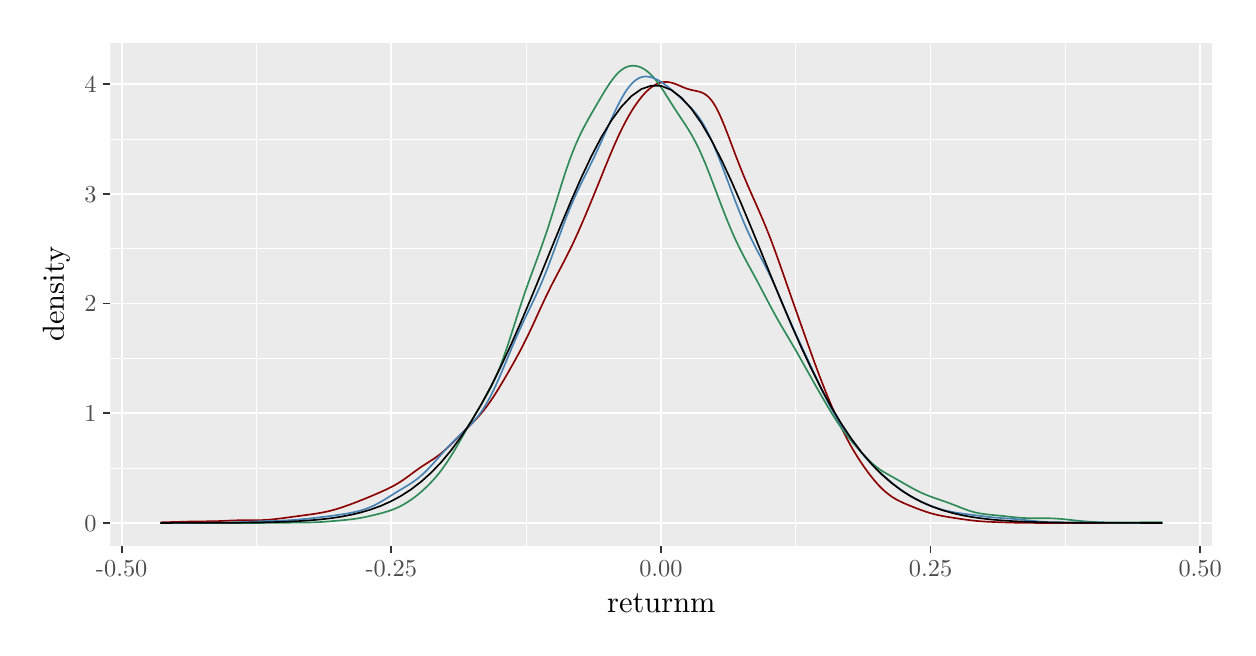
\begin{tikzpicture}[x=1pt,y=1pt]
\definecolor{fillColor}{RGB}{255,255,255}
\path[use as bounding box,fill=fillColor,fill opacity=0.00] (0,0) rectangle (433.62,216.81);
\begin{scope}
\path[clip] (  0.00,  0.00) rectangle (433.62,216.81);
\definecolor{drawColor}{RGB}{255,255,255}
\definecolor{fillColor}{RGB}{255,255,255}

\path[draw=drawColor,line width= 0.6pt,line join=round,line cap=round,fill=fillColor] (  0.00,  0.00) rectangle (433.62,216.81);
\end{scope}
\begin{scope}
\path[clip] ( 29.87, 29.59) rectangle (428.12,211.31);
\definecolor{fillColor}{gray}{0.92}

\path[fill=fillColor] ( 29.87, 29.59) rectangle (428.12,211.31);
\definecolor{drawColor}{RGB}{255,255,255}

\path[draw=drawColor,line width= 0.3pt,line join=round] ( 29.87, 57.67) --
	(428.12, 57.67);

\path[draw=drawColor,line width= 0.3pt,line join=round] ( 29.87, 97.30) --
	(428.12, 97.30);

\path[draw=drawColor,line width= 0.3pt,line join=round] ( 29.87,136.94) --
	(428.12,136.94);

\path[draw=drawColor,line width= 0.3pt,line join=round] ( 29.87,176.58) --
	(428.12,176.58);

\path[draw=drawColor,line width= 0.3pt,line join=round] ( 82.68, 29.59) --
	( 82.68,211.31);

\path[draw=drawColor,line width= 0.3pt,line join=round] (180.11, 29.59) --
	(180.11,211.31);

\path[draw=drawColor,line width= 0.3pt,line join=round] (277.54, 29.59) --
	(277.54,211.31);

\path[draw=drawColor,line width= 0.3pt,line join=round] (374.97, 29.59) --
	(374.97,211.31);

\path[draw=drawColor,line width= 0.6pt,line join=round] ( 29.87, 37.85) --
	(428.12, 37.85);

\path[draw=drawColor,line width= 0.6pt,line join=round] ( 29.87, 77.49) --
	(428.12, 77.49);

\path[draw=drawColor,line width= 0.6pt,line join=round] ( 29.87,117.12) --
	(428.12,117.12);

\path[draw=drawColor,line width= 0.6pt,line join=round] ( 29.87,156.76) --
	(428.12,156.76);

\path[draw=drawColor,line width= 0.6pt,line join=round] ( 29.87,196.40) --
	(428.12,196.40);

\path[draw=drawColor,line width= 0.6pt,line join=round] ( 33.97, 29.59) --
	( 33.97,211.31);

\path[draw=drawColor,line width= 0.6pt,line join=round] (131.40, 29.59) --
	(131.40,211.31);

\path[draw=drawColor,line width= 0.6pt,line join=round] (228.83, 29.59) --
	(228.83,211.31);

\path[draw=drawColor,line width= 0.6pt,line join=round] (326.26, 29.59) --
	(326.26,211.31);

\path[draw=drawColor,line width= 0.6pt,line join=round] (423.69, 29.59) --
	(423.69,211.31);
\definecolor{drawColor}{RGB}{139,0,0}

\path[draw=drawColor,line width= 0.6pt,line join=round] ( 47.97, 38.05) --
	( 48.68, 38.07) --
	( 49.39, 38.09) --
	( 50.10, 38.11) --
	( 50.81, 38.13) --
	( 51.51, 38.15) --
	( 52.22, 38.17) --
	( 52.93, 38.19) --
	( 53.64, 38.21) --
	( 54.35, 38.23) --
	( 55.06, 38.25) --
	( 55.76, 38.27) --
	( 56.47, 38.29) --
	( 57.18, 38.31) --
	( 57.89, 38.33) --
	( 58.60, 38.35) --
	( 59.31, 38.36) --
	( 60.02, 38.37) --
	( 60.72, 38.39) --
	( 61.43, 38.40) --
	( 62.14, 38.40) --
	( 62.85, 38.41) --
	( 63.56, 38.42) --
	( 64.27, 38.42) --
	( 64.98, 38.43) --
	( 65.68, 38.44) --
	( 66.39, 38.45) --
	( 67.10, 38.46) --
	( 67.81, 38.48) --
	( 68.52, 38.50) --
	( 69.23, 38.52) --
	( 69.93, 38.55) --
	( 70.64, 38.58) --
	( 71.35, 38.61) --
	( 72.06, 38.65) --
	( 72.77, 38.68) --
	( 73.48, 38.72) --
	( 74.19, 38.74) --
	( 74.89, 38.77) --
	( 75.60, 38.79) --
	( 76.31, 38.81) --
	( 77.02, 38.82) --
	( 77.73, 38.82) --
	( 78.44, 38.82) --
	( 79.15, 38.82) --
	( 79.85, 38.82) --
	( 80.56, 38.81) --
	( 81.27, 38.81) --
	( 81.98, 38.81) --
	( 82.69, 38.82) --
	( 83.40, 38.83) --
	( 84.10, 38.85) --
	( 84.81, 38.87) --
	( 85.52, 38.91) --
	( 86.23, 38.95) --
	( 86.94, 39.00) --
	( 87.65, 39.06) --
	( 88.36, 39.13) --
	( 89.06, 39.20) --
	( 89.77, 39.28) --
	( 90.48, 39.37) --
	( 91.19, 39.45) --
	( 91.90, 39.54) --
	( 92.61, 39.63) --
	( 93.32, 39.73) --
	( 94.02, 39.82) --
	( 94.73, 39.92) --
	( 95.44, 40.02) --
	( 96.15, 40.11) --
	( 96.86, 40.21) --
	( 97.57, 40.30) --
	( 98.28, 40.40) --
	( 98.98, 40.49) --
	( 99.69, 40.59) --
	(100.40, 40.68) --
	(101.11, 40.78) --
	(101.82, 40.87) --
	(102.53, 40.97) --
	(103.23, 41.07) --
	(103.94, 41.18) --
	(104.65, 41.29) --
	(105.36, 41.41) --
	(106.07, 41.53) --
	(106.78, 41.67) --
	(107.49, 41.81) --
	(108.19, 41.96) --
	(108.90, 42.13) --
	(109.61, 42.31) --
	(110.32, 42.49) --
	(111.03, 42.69) --
	(111.74, 42.90) --
	(112.45, 43.12) --
	(113.15, 43.35) --
	(113.86, 43.58) --
	(114.57, 43.83) --
	(115.28, 44.08) --
	(115.99, 44.33) --
	(116.70, 44.59) --
	(117.40, 44.85) --
	(118.11, 45.12) --
	(118.82, 45.39) --
	(119.53, 45.67) --
	(120.24, 45.95) --
	(120.95, 46.23) --
	(121.66, 46.51) --
	(122.36, 46.80) --
	(123.07, 47.10) --
	(123.78, 47.39) --
	(124.49, 47.69) --
	(125.20, 48.00) --
	(125.91, 48.30) --
	(126.62, 48.61) --
	(127.32, 48.92) --
	(128.03, 49.23) --
	(128.74, 49.55) --
	(129.45, 49.88) --
	(130.16, 50.21) --
	(130.87, 50.56) --
	(131.57, 50.92) --
	(132.28, 51.30) --
	(132.99, 51.69) --
	(133.70, 52.11) --
	(134.41, 52.55) --
	(135.12, 53.01) --
	(135.83, 53.49) --
	(136.53, 53.98) --
	(137.24, 54.49) --
	(137.95, 55.01) --
	(138.66, 55.54) --
	(139.37, 56.06) --
	(140.08, 56.58) --
	(140.79, 57.09) --
	(141.49, 57.59) --
	(142.20, 58.08) --
	(142.91, 58.55) --
	(143.62, 59.02) --
	(144.33, 59.47) --
	(145.04, 59.92) --
	(145.74, 60.38) --
	(146.45, 60.84) --
	(147.16, 61.32) --
	(147.87, 61.83) --
	(148.58, 62.35) --
	(149.29, 62.91) --
	(150.00, 63.49) --
	(150.70, 64.10) --
	(151.41, 64.74) --
	(152.12, 65.40) --
	(152.83, 66.09) --
	(153.54, 66.78) --
	(154.25, 67.49) --
	(154.96, 68.20) --
	(155.66, 68.92) --
	(156.37, 69.63) --
	(157.08, 70.34) --
	(157.79, 71.05) --
	(158.50, 71.76) --
	(159.21, 72.46) --
	(159.92, 73.17) --
	(160.62, 73.89) --
	(161.33, 74.62) --
	(162.04, 75.37) --
	(162.75, 76.14) --
	(163.46, 76.94) --
	(164.17, 77.77) --
	(164.87, 78.64) --
	(165.58, 79.56) --
	(166.29, 80.51) --
	(167.00, 81.51) --
	(167.71, 82.54) --
	(168.42, 83.61) --
	(169.13, 84.72) --
	(169.83, 85.85) --
	(170.54, 87.01) --
	(171.25, 88.20) --
	(171.96, 89.39) --
	(172.67, 90.60) --
	(173.38, 91.82) --
	(174.09, 93.05) --
	(174.79, 94.30) --
	(175.50, 95.55) --
	(176.21, 96.82) --
	(176.92, 98.11) --
	(177.63, 99.43) --
	(178.34,100.77) --
	(179.04,102.15) --
	(179.75,103.55) --
	(180.46,104.99) --
	(181.17,106.46) --
	(181.88,107.96) --
	(182.59,109.48) --
	(183.30,111.02) --
	(184.00,112.57) --
	(184.71,114.12) --
	(185.42,115.66) --
	(186.13,117.19) --
	(186.84,118.70) --
	(187.55,120.18) --
	(188.26,121.63) --
	(188.96,123.06) --
	(189.67,124.46) --
	(190.38,125.83) --
	(191.09,127.18) --
	(191.80,128.53) --
	(192.51,129.87) --
	(193.21,131.22) --
	(193.92,132.57) --
	(194.63,133.95) --
	(195.34,135.36) --
	(196.05,136.79) --
	(196.76,138.26) --
	(197.47,139.77) --
	(198.17,141.31) --
	(198.88,142.88) --
	(199.59,144.49) --
	(200.30,146.11) --
	(201.01,147.77) --
	(201.72,149.44) --
	(202.43,151.13) --
	(203.13,152.83) --
	(203.84,154.54) --
	(204.55,156.27) --
	(205.26,158.01) --
	(205.97,159.75) --
	(206.68,161.50) --
	(207.39,163.25) --
	(208.09,165.00) --
	(208.80,166.75) --
	(209.51,168.48) --
	(210.22,170.20) --
	(210.93,171.89) --
	(211.64,173.54) --
	(212.34,175.16) --
	(213.05,176.74) --
	(213.76,178.27) --
	(214.47,179.75) --
	(215.18,181.18) --
	(215.89,182.55) --
	(216.60,183.86) --
	(217.30,185.11) --
	(218.01,186.31) --
	(218.72,187.45) --
	(219.43,188.54) --
	(220.14,189.57) --
	(220.85,190.54) --
	(221.56,191.45) --
	(222.26,192.30) --
	(222.97,193.09) --
	(223.68,193.80) --
	(224.39,194.46) --
	(225.10,195.05) --
	(225.81,195.57) --
	(226.51,196.02) --
	(227.22,196.40) --
	(227.93,196.70) --
	(228.64,196.94) --
	(229.35,197.10) --
	(230.06,197.18) --
	(230.77,197.19) --
	(231.47,197.14) --
	(232.18,197.02) --
	(232.89,196.84) --
	(233.60,196.62) --
	(234.31,196.36) --
	(235.02,196.07) --
	(235.73,195.76) --
	(236.43,195.46) --
	(237.14,195.17) --
	(237.85,194.90) --
	(238.56,194.66) --
	(239.27,194.45) --
	(239.98,194.27) --
	(240.68,194.12) --
	(241.39,193.97) --
	(242.10,193.82) --
	(242.81,193.64) --
	(243.52,193.40) --
	(244.23,193.08) --
	(244.94,192.65) --
	(245.64,192.11) --
	(246.35,191.43) --
	(247.06,190.59) --
	(247.77,189.60) --
	(248.48,188.46) --
	(249.19,187.14) --
	(249.90,185.69) --
	(250.60,184.12) --
	(251.31,182.44) --
	(252.02,180.68) --
	(252.73,178.86) --
	(253.44,177.00) --
	(254.15,175.12) --
	(254.85,173.23) --
	(255.56,171.35) --
	(256.27,169.49) --
	(256.98,167.66) --
	(257.69,165.87) --
	(258.40,164.11) --
	(259.11,162.39) --
	(259.81,160.71) --
	(260.52,159.06) --
	(261.23,157.44) --
	(261.94,155.84) --
	(262.65,154.24) --
	(263.36,152.65) --
	(264.07,151.05) --
	(264.77,149.42) --
	(265.48,147.78) --
	(266.19,146.09) --
	(266.90,144.37) --
	(267.61,142.60) --
	(268.32,140.79) --
	(269.03,138.92) --
	(269.73,137.02) --
	(270.44,135.08) --
	(271.15,133.10) --
	(271.86,131.10) --
	(272.57,129.09) --
	(273.28,127.06) --
	(273.98,125.03) --
	(274.69,122.99) --
	(275.40,120.96) --
	(276.11,118.93) --
	(276.82,116.91) --
	(277.53,114.90) --
	(278.24,112.89) --
	(278.94,110.89) --
	(279.65,108.88) --
	(280.36,106.88) --
	(281.07,104.88) --
	(281.78,102.89) --
	(282.49,100.91) --
	(283.20, 98.93) --
	(283.90, 96.97) --
	(284.61, 95.03) --
	(285.32, 93.12) --
	(286.03, 91.23) --
	(286.74, 89.37) --
	(287.45, 87.55) --
	(288.15, 85.76) --
	(288.86, 84.02) --
	(289.57, 82.30) --
	(290.28, 80.62) --
	(290.99, 78.97) --
	(291.70, 77.36) --
	(292.41, 75.78) --
	(293.11, 74.24) --
	(293.82, 72.74) --
	(294.53, 71.28) --
	(295.24, 69.86) --
	(295.95, 68.48) --
	(296.66, 67.15) --
	(297.37, 65.86) --
	(298.07, 64.62) --
	(298.78, 63.42) --
	(299.49, 62.26) --
	(300.20, 61.13) --
	(300.91, 60.05) --
	(301.62, 59.00) --
	(302.32, 57.98) --
	(303.03, 56.99) --
	(303.74, 56.02) --
	(304.45, 55.09) --
	(305.16, 54.19) --
	(305.87, 53.32) --
	(306.58, 52.49) --
	(307.28, 51.70) --
	(307.99, 50.95) --
	(308.70, 50.24) --
	(309.41, 49.57) --
	(310.12, 48.96) --
	(310.83, 48.38) --
	(311.54, 47.84) --
	(312.24, 47.35) --
	(312.95, 46.89) --
	(313.66, 46.47) --
	(314.37, 46.08) --
	(315.08, 45.72) --
	(315.79, 45.38) --
	(316.49, 45.05) --
	(317.20, 44.74) --
	(317.91, 44.44) --
	(318.62, 44.15) --
	(319.33, 43.86) --
	(320.04, 43.58) --
	(320.75, 43.30) --
	(321.45, 43.03) --
	(322.16, 42.76) --
	(322.87, 42.50) --
	(323.58, 42.25) --
	(324.29, 42.00) --
	(325.00, 41.77) --
	(325.71, 41.55) --
	(326.41, 41.33) --
	(327.12, 41.14) --
	(327.83, 40.95) --
	(328.54, 40.78) --
	(329.25, 40.63) --
	(329.96, 40.48) --
	(330.67, 40.34) --
	(331.37, 40.21) --
	(332.08, 40.09) --
	(332.79, 39.97) --
	(333.50, 39.85) --
	(334.21, 39.74) --
	(334.92, 39.63) --
	(335.62, 39.53) --
	(336.33, 39.42) --
	(337.04, 39.31) --
	(337.75, 39.21) --
	(338.46, 39.11) --
	(339.17, 39.01) --
	(339.88, 38.92) --
	(340.58, 38.83) --
	(341.29, 38.74) --
	(342.00, 38.66) --
	(342.71, 38.59) --
	(343.42, 38.52) --
	(344.13, 38.46) --
	(344.84, 38.41) --
	(345.54, 38.36) --
	(346.25, 38.32) --
	(346.96, 38.28) --
	(347.67, 38.24) --
	(348.38, 38.21) --
	(349.09, 38.18) --
	(349.79, 38.15) --
	(350.50, 38.13) --
	(351.21, 38.10) --
	(351.92, 38.08) --
	(352.63, 38.05) --
	(353.34, 38.03) --
	(354.05, 38.01) --
	(354.75, 37.99) --
	(355.46, 37.97) --
	(356.17, 37.95) --
	(356.88, 37.93) --
	(357.59, 37.92) --
	(358.30, 37.91) --
	(359.01, 37.89) --
	(359.71, 37.88) --
	(360.42, 37.88) --
	(361.13, 37.87) --
	(361.84, 37.86) --
	(362.55, 37.86) --
	(363.26, 37.86) --
	(363.96, 37.85) --
	(364.67, 37.85) --
	(365.38, 37.85) --
	(366.09, 37.85) --
	(366.80, 37.85) --
	(367.51, 37.85) --
	(368.22, 37.85) --
	(368.92, 37.85) --
	(369.63, 37.85) --
	(370.34, 37.85) --
	(371.05, 37.85) --
	(371.76, 37.85) --
	(372.47, 37.85) --
	(373.18, 37.85) --
	(373.88, 37.85) --
	(374.59, 37.85) --
	(375.30, 37.85) --
	(376.01, 37.85) --
	(376.72, 37.85) --
	(377.43, 37.85) --
	(378.13, 37.85) --
	(378.84, 37.85) --
	(379.55, 37.85) --
	(380.26, 37.85) --
	(380.97, 37.85) --
	(381.68, 37.85) --
	(382.39, 37.85) --
	(383.09, 37.85) --
	(383.80, 37.85) --
	(384.51, 37.85) --
	(385.22, 37.85) --
	(385.93, 37.85) --
	(386.64, 37.85) --
	(387.35, 37.85) --
	(388.05, 37.85) --
	(388.76, 37.85) --
	(389.47, 37.85) --
	(390.18, 37.85) --
	(390.89, 37.85) --
	(391.60, 37.85) --
	(392.31, 37.85) --
	(393.01, 37.85) --
	(393.72, 37.85) --
	(394.43, 37.85) --
	(395.14, 37.85) --
	(395.85, 37.85) --
	(396.56, 37.85) --
	(397.26, 37.85) --
	(397.97, 37.85) --
	(398.68, 37.85) --
	(399.39, 37.85) --
	(400.10, 37.85) --
	(400.81, 37.85) --
	(401.52, 37.85) --
	(402.22, 37.85) --
	(402.93, 37.85) --
	(403.64, 37.85) --
	(404.35, 37.85) --
	(405.06, 37.85) --
	(405.77, 37.85) --
	(406.48, 37.85) --
	(407.18, 37.85) --
	(407.89, 37.85) --
	(408.60, 37.85) --
	(409.31, 37.85) --
	(410.02, 37.85);
\definecolor{drawColor}{RGB}{46,139,87}

\path[draw=drawColor,line width= 0.6pt,line join=round] ( 47.97, 37.85) --
	( 48.68, 37.85) --
	( 49.39, 37.85) --
	( 50.10, 37.85) --
	( 50.81, 37.85) --
	( 51.51, 37.85) --
	( 52.22, 37.85) --
	( 52.93, 37.85) --
	( 53.64, 37.85) --
	( 54.35, 37.85) --
	( 55.06, 37.85) --
	( 55.76, 37.85) --
	( 56.47, 37.85) --
	( 57.18, 37.85) --
	( 57.89, 37.85) --
	( 58.60, 37.85) --
	( 59.31, 37.85) --
	( 60.02, 37.85) --
	( 60.72, 37.85) --
	( 61.43, 37.85) --
	( 62.14, 37.85) --
	( 62.85, 37.85) --
	( 63.56, 37.85) --
	( 64.27, 37.85) --
	( 64.98, 37.85) --
	( 65.68, 37.85) --
	( 66.39, 37.85) --
	( 67.10, 37.85) --
	( 67.81, 37.85) --
	( 68.52, 37.85) --
	( 69.23, 37.85) --
	( 69.93, 37.85) --
	( 70.64, 37.85) --
	( 71.35, 37.85) --
	( 72.06, 37.85) --
	( 72.77, 37.85) --
	( 73.48, 37.85) --
	( 74.19, 37.85) --
	( 74.89, 37.85) --
	( 75.60, 37.85) --
	( 76.31, 37.85) --
	( 77.02, 37.85) --
	( 77.73, 37.85) --
	( 78.44, 37.85) --
	( 79.15, 37.85) --
	( 79.85, 37.85) --
	( 80.56, 37.85) --
	( 81.27, 37.85) --
	( 81.98, 37.85) --
	( 82.69, 37.85) --
	( 83.40, 37.85) --
	( 84.10, 37.85) --
	( 84.81, 37.85) --
	( 85.52, 37.85) --
	( 86.23, 37.86) --
	( 86.94, 37.86) --
	( 87.65, 37.87) --
	( 88.36, 37.87) --
	( 89.06, 37.88) --
	( 89.77, 37.88) --
	( 90.48, 37.89) --
	( 91.19, 37.90) --
	( 91.90, 37.91) --
	( 92.61, 37.92) --
	( 93.32, 37.92) --
	( 94.02, 37.93) --
	( 94.73, 37.94) --
	( 95.44, 37.95) --
	( 96.15, 37.96) --
	( 96.86, 37.97) --
	( 97.57, 37.97) --
	( 98.28, 37.98) --
	( 98.98, 37.99) --
	( 99.69, 37.99) --
	(100.40, 38.00) --
	(101.11, 38.01) --
	(101.82, 38.02) --
	(102.53, 38.04) --
	(103.23, 38.06) --
	(103.94, 38.08) --
	(104.65, 38.11) --
	(105.36, 38.15) --
	(106.07, 38.19) --
	(106.78, 38.23) --
	(107.49, 38.28) --
	(108.19, 38.34) --
	(108.90, 38.40) --
	(109.61, 38.46) --
	(110.32, 38.52) --
	(111.03, 38.58) --
	(111.74, 38.65) --
	(112.45, 38.71) --
	(113.15, 38.77) --
	(113.86, 38.84) --
	(114.57, 38.90) --
	(115.28, 38.97) --
	(115.99, 39.05) --
	(116.70, 39.13) --
	(117.40, 39.21) --
	(118.11, 39.31) --
	(118.82, 39.41) --
	(119.53, 39.53) --
	(120.24, 39.65) --
	(120.95, 39.78) --
	(121.66, 39.92) --
	(122.36, 40.07) --
	(123.07, 40.23) --
	(123.78, 40.39) --
	(124.49, 40.55) --
	(125.20, 40.72) --
	(125.91, 40.89) --
	(126.62, 41.07) --
	(127.32, 41.25) --
	(128.03, 41.44) --
	(128.74, 41.64) --
	(129.45, 41.84) --
	(130.16, 42.06) --
	(130.87, 42.30) --
	(131.57, 42.55) --
	(132.28, 42.82) --
	(132.99, 43.11) --
	(133.70, 43.42) --
	(134.41, 43.76) --
	(135.12, 44.12) --
	(135.83, 44.51) --
	(136.53, 44.92) --
	(137.24, 45.36) --
	(137.95, 45.82) --
	(138.66, 46.31) --
	(139.37, 46.82) --
	(140.08, 47.35) --
	(140.79, 47.91) --
	(141.49, 48.49) --
	(142.20, 49.10) --
	(142.91, 49.72) --
	(143.62, 50.38) --
	(144.33, 51.06) --
	(145.04, 51.76) --
	(145.74, 52.50) --
	(146.45, 53.26) --
	(147.16, 54.05) --
	(147.87, 54.89) --
	(148.58, 55.75) --
	(149.29, 56.66) --
	(150.00, 57.60) --
	(150.70, 58.60) --
	(151.41, 59.63) --
	(152.12, 60.70) --
	(152.83, 61.81) --
	(153.54, 62.95) --
	(154.25, 64.12) --
	(154.96, 65.32) --
	(155.66, 66.54) --
	(156.37, 67.77) --
	(157.08, 69.01) --
	(157.79, 70.26) --
	(158.50, 71.50) --
	(159.21, 72.73) --
	(159.92, 73.96) --
	(160.62, 75.17) --
	(161.33, 76.38) --
	(162.04, 77.57) --
	(162.75, 78.75) --
	(163.46, 79.93) --
	(164.17, 81.11) --
	(164.87, 82.31) --
	(165.58, 83.54) --
	(166.29, 84.81) --
	(167.00, 86.14) --
	(167.71, 87.52) --
	(168.42, 88.99) --
	(169.13, 90.53) --
	(169.83, 92.18) --
	(170.54, 93.93) --
	(171.25, 95.77) --
	(171.96, 97.70) --
	(172.67, 99.72) --
	(173.38,101.80) --
	(174.09,103.94) --
	(174.79,106.13) --
	(175.50,108.34) --
	(176.21,110.56) --
	(176.92,112.77) --
	(177.63,114.96) --
	(178.34,117.11) --
	(179.04,119.23) --
	(179.75,121.30) --
	(180.46,123.33) --
	(181.17,125.32) --
	(181.88,127.28) --
	(182.59,129.21) --
	(183.30,131.13) --
	(184.00,133.05) --
	(184.71,134.99) --
	(185.42,136.96) --
	(186.13,138.97) --
	(186.84,141.02) --
	(187.55,143.12) --
	(188.26,145.28) --
	(188.96,147.48) --
	(189.67,149.73) --
	(190.38,152.02) --
	(191.09,154.32) --
	(191.80,156.62) --
	(192.51,158.90) --
	(193.21,161.16) --
	(193.92,163.36) --
	(194.63,165.51) --
	(195.34,167.57) --
	(196.05,169.56) --
	(196.76,171.43) --
	(197.47,173.22) --
	(198.17,174.90) --
	(198.88,176.50) --
	(199.59,178.02) --
	(200.30,179.47) --
	(201.01,180.85) --
	(201.72,182.17) --
	(202.43,183.46) --
	(203.13,184.72) --
	(203.84,185.96) --
	(204.55,187.18) --
	(205.26,188.40) --
	(205.97,189.62) --
	(206.68,190.83) --
	(207.39,192.02) --
	(208.09,193.20) --
	(208.80,194.36) --
	(209.51,195.48) --
	(210.22,196.55) --
	(210.93,197.56) --
	(211.64,198.51) --
	(212.34,199.37) --
	(213.05,200.16) --
	(213.76,200.85) --
	(214.47,201.45) --
	(215.18,201.96) --
	(215.89,202.36) --
	(216.60,202.67) --
	(217.30,202.88) --
	(218.01,203.01) --
	(218.72,203.05) --
	(219.43,203.01) --
	(220.14,202.90) --
	(220.85,202.71) --
	(221.56,202.45) --
	(222.26,202.11) --
	(222.97,201.69) --
	(223.68,201.19) --
	(224.39,200.61) --
	(225.10,199.95) --
	(225.81,199.22) --
	(226.51,198.42) --
	(227.22,197.54) --
	(227.93,196.60) --
	(228.64,195.60) --
	(229.35,194.55) --
	(230.06,193.46) --
	(230.77,192.35) --
	(231.47,191.23) --
	(232.18,190.10) --
	(232.89,188.98) --
	(233.60,187.87) --
	(234.31,186.77) --
	(235.02,185.70) --
	(235.73,184.63) --
	(236.43,183.57) --
	(237.14,182.50) --
	(237.85,181.42) --
	(238.56,180.31) --
	(239.27,179.15) --
	(239.98,177.95) --
	(240.68,176.68) --
	(241.39,175.35) --
	(242.10,173.93) --
	(242.81,172.44) --
	(243.52,170.86) --
	(244.23,169.22) --
	(244.94,167.52) --
	(245.64,165.76) --
	(246.35,163.95) --
	(247.06,162.11) --
	(247.77,160.25) --
	(248.48,158.36) --
	(249.19,156.48) --
	(249.90,154.60) --
	(250.60,152.73) --
	(251.31,150.89) --
	(252.02,149.08) --
	(252.73,147.30) --
	(253.44,145.57) --
	(254.15,143.88) --
	(254.85,142.25) --
	(255.56,140.68) --
	(256.27,139.16) --
	(256.98,137.69) --
	(257.69,136.27) --
	(258.40,134.89) --
	(259.11,133.54) --
	(259.81,132.21) --
	(260.52,130.91) --
	(261.23,129.61) --
	(261.94,128.31) --
	(262.65,127.01) --
	(263.36,125.69) --
	(264.07,124.37) --
	(264.77,123.03) --
	(265.48,121.68) --
	(266.19,120.33) --
	(266.90,118.98) --
	(267.61,117.63) --
	(268.32,116.29) --
	(269.03,114.97) --
	(269.73,113.67) --
	(270.44,112.39) --
	(271.15,111.13) --
	(271.86,109.89) --
	(272.57,108.67) --
	(273.28,107.47) --
	(273.98,106.27) --
	(274.69,105.08) --
	(275.40,103.88) --
	(276.11,102.68) --
	(276.82,101.47) --
	(277.53,100.25) --
	(278.24, 99.01) --
	(278.94, 97.76) --
	(279.65, 96.51) --
	(280.36, 95.24) --
	(281.07, 93.97) --
	(281.78, 92.70) --
	(282.49, 91.44) --
	(283.20, 90.17) --
	(283.90, 88.91) --
	(284.61, 87.66) --
	(285.32, 86.41) --
	(286.03, 85.17) --
	(286.74, 83.94) --
	(287.45, 82.71) --
	(288.15, 81.50) --
	(288.86, 80.30) --
	(289.57, 79.11) --
	(290.28, 77.94) --
	(290.99, 76.79) --
	(291.70, 75.67) --
	(292.41, 74.58) --
	(293.11, 73.52) --
	(293.82, 72.49) --
	(294.53, 71.49) --
	(295.24, 70.53) --
	(295.95, 69.60) --
	(296.66, 68.69) --
	(297.37, 67.81) --
	(298.07, 66.96) --
	(298.78, 66.12) --
	(299.49, 65.29) --
	(300.20, 64.48) --
	(300.91, 63.69) --
	(301.62, 62.91) --
	(302.32, 62.15) --
	(303.03, 61.42) --
	(303.74, 60.71) --
	(304.45, 60.03) --
	(305.16, 59.38) --
	(305.87, 58.77) --
	(306.58, 58.19) --
	(307.28, 57.66) --
	(307.99, 57.15) --
	(308.70, 56.68) --
	(309.41, 56.24) --
	(310.12, 55.81) --
	(310.83, 55.41) --
	(311.54, 55.01) --
	(312.24, 54.61) --
	(312.95, 54.22) --
	(313.66, 53.82) --
	(314.37, 53.42) --
	(315.08, 53.02) --
	(315.79, 52.61) --
	(316.49, 52.20) --
	(317.20, 51.79) --
	(317.91, 51.38) --
	(318.62, 50.98) --
	(319.33, 50.58) --
	(320.04, 50.20) --
	(320.75, 49.82) --
	(321.45, 49.46) --
	(322.16, 49.11) --
	(322.87, 48.78) --
	(323.58, 48.46) --
	(324.29, 48.16) --
	(325.00, 47.87) --
	(325.71, 47.59) --
	(326.41, 47.32) --
	(327.12, 47.06) --
	(327.83, 46.81) --
	(328.54, 46.56) --
	(329.25, 46.32) --
	(329.96, 46.08) --
	(330.67, 45.83) --
	(331.37, 45.59) --
	(332.08, 45.34) --
	(332.79, 45.08) --
	(333.50, 44.82) --
	(334.21, 44.55) --
	(334.92, 44.27) --
	(335.62, 43.99) --
	(336.33, 43.71) --
	(337.04, 43.43) --
	(337.75, 43.16) --
	(338.46, 42.89) --
	(339.17, 42.63) --
	(339.88, 42.38) --
	(340.58, 42.15) --
	(341.29, 41.94) --
	(342.00, 41.75) --
	(342.71, 41.58) --
	(343.42, 41.43) --
	(344.13, 41.29) --
	(344.84, 41.17) --
	(345.54, 41.07) --
	(346.25, 40.98) --
	(346.96, 40.90) --
	(347.67, 40.82) --
	(348.38, 40.75) --
	(349.09, 40.69) --
	(349.79, 40.62) --
	(350.50, 40.55) --
	(351.21, 40.48) --
	(351.92, 40.41) --
	(352.63, 40.34) --
	(353.34, 40.26) --
	(354.05, 40.18) --
	(354.75, 40.10) --
	(355.46, 40.02) --
	(356.17, 39.94) --
	(356.88, 39.87) --
	(357.59, 39.80) --
	(358.30, 39.74) --
	(359.01, 39.69) --
	(359.71, 39.64) --
	(360.42, 39.61) --
	(361.13, 39.58) --
	(361.84, 39.56) --
	(362.55, 39.55) --
	(363.26, 39.54) --
	(363.96, 39.54) --
	(364.67, 39.54) --
	(365.38, 39.54) --
	(366.09, 39.55) --
	(366.80, 39.55) --
	(367.51, 39.55) --
	(368.22, 39.54) --
	(368.92, 39.53) --
	(369.63, 39.51) --
	(370.34, 39.49) --
	(371.05, 39.45) --
	(371.76, 39.41) --
	(372.47, 39.36) --
	(373.18, 39.31) --
	(373.88, 39.25) --
	(374.59, 39.18) --
	(375.30, 39.10) --
	(376.01, 39.03) --
	(376.72, 38.95) --
	(377.43, 38.87) --
	(378.13, 38.79) --
	(378.84, 38.71) --
	(379.55, 38.64) --
	(380.26, 38.57) --
	(380.97, 38.50) --
	(381.68, 38.44) --
	(382.39, 38.38) --
	(383.09, 38.33) --
	(383.80, 38.28) --
	(384.51, 38.24) --
	(385.22, 38.20) --
	(385.93, 38.17) --
	(386.64, 38.14) --
	(387.35, 38.11) --
	(388.05, 38.09) --
	(388.76, 38.07) --
	(389.47, 38.05) --
	(390.18, 38.04) --
	(390.89, 38.02) --
	(391.60, 38.01) --
	(392.31, 38.01) --
	(393.01, 38.00) --
	(393.72, 38.00) --
	(394.43, 38.00) --
	(395.14, 38.00) --
	(395.85, 38.00) --
	(396.56, 38.01) --
	(397.26, 38.01) --
	(397.97, 38.02) --
	(398.68, 38.03) --
	(399.39, 38.04) --
	(400.10, 38.05) --
	(400.81, 38.05) --
	(401.52, 38.06) --
	(402.22, 38.07) --
	(402.93, 38.08) --
	(403.64, 38.09) --
	(404.35, 38.09) --
	(405.06, 38.10) --
	(405.77, 38.10) --
	(406.48, 38.10) --
	(407.18, 38.10) --
	(407.89, 38.09) --
	(408.60, 38.09) --
	(409.31, 38.08) --
	(410.02, 38.07);
\definecolor{drawColor}{RGB}{70,130,180}

\path[draw=drawColor,line width= 0.6pt,line join=round] ( 47.97, 37.85) --
	( 48.68, 37.85) --
	( 49.39, 37.85) --
	( 50.10, 37.85) --
	( 50.81, 37.85) --
	( 51.51, 37.85) --
	( 52.22, 37.85) --
	( 52.93, 37.85) --
	( 53.64, 37.85) --
	( 54.35, 37.85) --
	( 55.06, 37.85) --
	( 55.76, 37.85) --
	( 56.47, 37.85) --
	( 57.18, 37.85) --
	( 57.89, 37.85) --
	( 58.60, 37.85) --
	( 59.31, 37.85) --
	( 60.02, 37.86) --
	( 60.72, 37.86) --
	( 61.43, 37.86) --
	( 62.14, 37.87) --
	( 62.85, 37.87) --
	( 63.56, 37.88) --
	( 64.27, 37.89) --
	( 64.98, 37.90) --
	( 65.68, 37.91) --
	( 66.39, 37.92) --
	( 67.10, 37.93) --
	( 67.81, 37.94) --
	( 68.52, 37.95) --
	( 69.23, 37.96) --
	( 69.93, 37.97) --
	( 70.64, 37.99) --
	( 71.35, 38.00) --
	( 72.06, 38.01) --
	( 72.77, 38.03) --
	( 73.48, 38.04) --
	( 74.19, 38.06) --
	( 74.89, 38.08) --
	( 75.60, 38.10) --
	( 76.31, 38.12) --
	( 77.02, 38.15) --
	( 77.73, 38.18) --
	( 78.44, 38.21) --
	( 79.15, 38.24) --
	( 79.85, 38.27) --
	( 80.56, 38.31) --
	( 81.27, 38.34) --
	( 81.98, 38.37) --
	( 82.69, 38.40) --
	( 83.40, 38.43) --
	( 84.10, 38.46) --
	( 84.81, 38.49) --
	( 85.52, 38.51) --
	( 86.23, 38.53) --
	( 86.94, 38.55) --
	( 87.65, 38.57) --
	( 88.36, 38.58) --
	( 89.06, 38.60) --
	( 89.77, 38.62) --
	( 90.48, 38.64) --
	( 91.19, 38.66) --
	( 91.90, 38.69) --
	( 92.61, 38.72) --
	( 93.32, 38.75) --
	( 94.02, 38.79) --
	( 94.73, 38.83) --
	( 95.44, 38.88) --
	( 96.15, 38.93) --
	( 96.86, 38.99) --
	( 97.57, 39.04) --
	( 98.28, 39.11) --
	( 98.98, 39.17) --
	( 99.69, 39.24) --
	(100.40, 39.31) --
	(101.11, 39.38) --
	(101.82, 39.45) --
	(102.53, 39.53) --
	(103.23, 39.61) --
	(103.94, 39.69) --
	(104.65, 39.77) --
	(105.36, 39.85) --
	(106.07, 39.94) --
	(106.78, 40.03) --
	(107.49, 40.11) --
	(108.19, 40.20) --
	(108.90, 40.30) --
	(109.61, 40.39) --
	(110.32, 40.48) --
	(111.03, 40.58) --
	(111.74, 40.68) --
	(112.45, 40.78) --
	(113.15, 40.88) --
	(113.86, 40.99) --
	(114.57, 41.10) --
	(115.28, 41.22) --
	(115.99, 41.35) --
	(116.70, 41.49) --
	(117.40, 41.63) --
	(118.11, 41.78) --
	(118.82, 41.95) --
	(119.53, 42.13) --
	(120.24, 42.32) --
	(120.95, 42.53) --
	(121.66, 42.76) --
	(122.36, 43.00) --
	(123.07, 43.27) --
	(123.78, 43.55) --
	(124.49, 43.86) --
	(125.20, 44.19) --
	(125.91, 44.55) --
	(126.62, 44.92) --
	(127.32, 45.31) --
	(128.03, 45.72) --
	(128.74, 46.15) --
	(129.45, 46.58) --
	(130.16, 47.02) --
	(130.87, 47.46) --
	(131.57, 47.91) --
	(132.28, 48.35) --
	(132.99, 48.79) --
	(133.70, 49.22) --
	(134.41, 49.65) --
	(135.12, 50.07) --
	(135.83, 50.50) --
	(136.53, 50.93) --
	(137.24, 51.36) --
	(137.95, 51.80) --
	(138.66, 52.26) --
	(139.37, 52.74) --
	(140.08, 53.25) --
	(140.79, 53.78) --
	(141.49, 54.35) --
	(142.20, 54.95) --
	(142.91, 55.59) --
	(143.62, 56.26) --
	(144.33, 56.96) --
	(145.04, 57.70) --
	(145.74, 58.46) --
	(146.45, 59.23) --
	(147.16, 60.02) --
	(147.87, 60.82) --
	(148.58, 61.62) --
	(149.29, 62.42) --
	(150.00, 63.21) --
	(150.70, 64.00) --
	(151.41, 64.76) --
	(152.12, 65.52) --
	(152.83, 66.26) --
	(153.54, 66.98) --
	(154.25, 67.69) --
	(154.96, 68.39) --
	(155.66, 69.08) --
	(156.37, 69.76) --
	(157.08, 70.44) --
	(157.79, 71.12) --
	(158.50, 71.81) --
	(159.21, 72.51) --
	(159.92, 73.23) --
	(160.62, 73.97) --
	(161.33, 74.75) --
	(162.04, 75.58) --
	(162.75, 76.46) --
	(163.46, 77.39) --
	(164.17, 78.40) --
	(164.87, 79.48) --
	(165.58, 80.64) --
	(166.29, 81.87) --
	(167.00, 83.17) --
	(167.71, 84.55) --
	(168.42, 85.99) --
	(169.13, 87.50) --
	(169.83, 89.06) --
	(170.54, 90.67) --
	(171.25, 92.32) --
	(171.96, 94.00) --
	(172.67, 95.69) --
	(173.38, 97.39) --
	(174.09, 99.09) --
	(174.79,100.79) --
	(175.50,102.46) --
	(176.21,104.11) --
	(176.92,105.74) --
	(177.63,107.32) --
	(178.34,108.88) --
	(179.04,110.41) --
	(179.75,111.91) --
	(180.46,113.39) --
	(181.17,114.86) --
	(181.88,116.33) --
	(182.59,117.81) --
	(183.30,119.30) --
	(184.00,120.83) --
	(184.71,122.40) --
	(185.42,124.02) --
	(186.13,125.69) --
	(186.84,127.41) --
	(187.55,129.19) --
	(188.26,131.02) --
	(188.96,132.90) --
	(189.67,134.81) --
	(190.38,136.76) --
	(191.09,138.71) --
	(191.80,140.67) --
	(192.51,142.61) --
	(193.21,144.53) --
	(193.92,146.42) --
	(194.63,148.26) --
	(195.34,150.06) --
	(196.05,151.79) --
	(196.76,153.47) --
	(197.47,155.10) --
	(198.17,156.66) --
	(198.88,158.19) --
	(199.59,159.67) --
	(200.30,161.13) --
	(201.01,162.56) --
	(201.72,163.98) --
	(202.43,165.40) --
	(203.13,166.83) --
	(203.84,168.27) --
	(204.55,169.74) --
	(205.26,171.23) --
	(205.97,172.75) --
	(206.68,174.29) --
	(207.39,175.85) --
	(208.09,177.44) --
	(208.80,179.03) --
	(209.51,180.62) --
	(210.22,182.21) --
	(210.93,183.78) --
	(211.64,185.33) --
	(212.34,186.83) --
	(213.05,188.28) --
	(213.76,189.68) --
	(214.47,191.01) --
	(215.18,192.26) --
	(215.89,193.43) --
	(216.60,194.48) --
	(217.30,195.44) --
	(218.01,196.29) --
	(218.72,197.02) --
	(219.43,197.65) --
	(220.14,198.16) --
	(220.85,198.56) --
	(221.56,198.86) --
	(222.26,199.05) --
	(222.97,199.14) --
	(223.68,199.14) --
	(224.39,199.07) --
	(225.10,198.92) --
	(225.81,198.71) --
	(226.51,198.44) --
	(227.22,198.12) --
	(227.93,197.76) --
	(228.64,197.35) --
	(229.35,196.89) --
	(230.06,196.40) --
	(230.77,195.88) --
	(231.47,195.32) --
	(232.18,194.75) --
	(232.89,194.15) --
	(233.60,193.53) --
	(234.31,192.90) --
	(235.02,192.27) --
	(235.73,191.62) --
	(236.43,190.98) --
	(237.14,190.32) --
	(237.85,189.66) --
	(238.56,188.98) --
	(239.27,188.28) --
	(239.98,187.54) --
	(240.68,186.76) --
	(241.39,185.93) --
	(242.10,185.02) --
	(242.81,184.03) --
	(243.52,182.96) --
	(244.23,181.79) --
	(244.94,180.53) --
	(245.64,179.17) --
	(246.35,177.73) --
	(247.06,176.21) --
	(247.77,174.61) --
	(248.48,172.94) --
	(249.19,171.21) --
	(249.90,169.43) --
	(250.60,167.62) --
	(251.31,165.77) --
	(252.02,163.91) --
	(252.73,162.02) --
	(253.44,160.13) --
	(254.15,158.24) --
	(254.85,156.36) --
	(255.56,154.50) --
	(256.27,152.66) --
	(256.98,150.85) --
	(257.69,149.08) --
	(258.40,147.36) --
	(259.11,145.69) --
	(259.81,144.08) --
	(260.52,142.52) --
	(261.23,141.01) --
	(261.94,139.55) --
	(262.65,138.14) --
	(263.36,136.76) --
	(264.07,135.41) --
	(264.77,134.06) --
	(265.48,132.71) --
	(266.19,131.35) --
	(266.90,129.96) --
	(267.61,128.55) --
	(268.32,127.09) --
	(269.03,125.60) --
	(269.73,124.06) --
	(270.44,122.49) --
	(271.15,120.88) --
	(271.86,119.25) --
	(272.57,117.60) --
	(273.28,115.94) --
	(273.98,114.28) --
	(274.69,112.63) --
	(275.40,111.00) --
	(276.11,109.39) --
	(276.82,107.80) --
	(277.53,106.24) --
	(278.24,104.69) --
	(278.94,103.17) --
	(279.65,101.65) --
	(280.36,100.14) --
	(281.07, 98.64) --
	(281.78, 97.12) --
	(282.49, 95.60) --
	(283.20, 94.08) --
	(283.90, 92.54) --
	(284.61, 91.01) --
	(285.32, 89.47) --
	(286.03, 87.95) --
	(286.74, 86.44) --
	(287.45, 84.96) --
	(288.15, 83.51) --
	(288.86, 82.10) --
	(289.57, 80.74) --
	(290.28, 79.43) --
	(290.99, 78.16) --
	(291.70, 76.94) --
	(292.41, 75.77) --
	(293.11, 74.64) --
	(293.82, 73.54) --
	(294.53, 72.48) --
	(295.24, 71.44) --
	(295.95, 70.43) --
	(296.66, 69.43) --
	(297.37, 68.45) --
	(298.07, 67.48) --
	(298.78, 66.53) --
	(299.49, 65.59) --
	(300.20, 64.66) --
	(300.91, 63.76) --
	(301.62, 62.88) --
	(302.32, 62.02) --
	(303.03, 61.19) --
	(303.74, 60.39) --
	(304.45, 59.61) --
	(305.16, 58.86) --
	(305.87, 58.14) --
	(306.58, 57.44) --
	(307.28, 56.76) --
	(307.99, 56.10) --
	(308.70, 55.45) --
	(309.41, 54.82) --
	(310.12, 54.20) --
	(310.83, 53.59) --
	(311.54, 52.99) --
	(312.24, 52.39) --
	(312.95, 51.82) --
	(313.66, 51.25) --
	(314.37, 50.70) --
	(315.08, 50.18) --
	(315.79, 49.67) --
	(316.49, 49.18) --
	(317.20, 48.70) --
	(317.91, 48.25) --
	(318.62, 47.82) --
	(319.33, 47.41) --
	(320.04, 47.01) --
	(320.75, 46.62) --
	(321.45, 46.26) --
	(322.16, 45.90) --
	(322.87, 45.56) --
	(323.58, 45.23) --
	(324.29, 44.91) --
	(325.00, 44.60) --
	(325.71, 44.30) --
	(326.41, 44.02) --
	(327.12, 43.74) --
	(327.83, 43.49) --
	(328.54, 43.24) --
	(329.25, 43.01) --
	(329.96, 42.79) --
	(330.67, 42.59) --
	(331.37, 42.40) --
	(332.08, 42.23) --
	(332.79, 42.07) --
	(333.50, 41.92) --
	(334.21, 41.78) --
	(334.92, 41.65) --
	(335.62, 41.54) --
	(336.33, 41.43) --
	(337.04, 41.32) --
	(337.75, 41.22) --
	(338.46, 41.13) --
	(339.17, 41.04) --
	(339.88, 40.95) --
	(340.58, 40.86) --
	(341.29, 40.77) --
	(342.00, 40.67) --
	(342.71, 40.58) --
	(343.42, 40.49) --
	(344.13, 40.40) --
	(344.84, 40.31) --
	(345.54, 40.22) --
	(346.25, 40.13) --
	(346.96, 40.05) --
	(347.67, 39.98) --
	(348.38, 39.90) --
	(349.09, 39.83) --
	(349.79, 39.77) --
	(350.50, 39.71) --
	(351.21, 39.66) --
	(351.92, 39.61) --
	(352.63, 39.56) --
	(353.34, 39.51) --
	(354.05, 39.46) --
	(354.75, 39.42) --
	(355.46, 39.36) --
	(356.17, 39.31) --
	(356.88, 39.25) --
	(357.59, 39.18) --
	(358.30, 39.12) --
	(359.01, 39.05) --
	(359.71, 38.97) --
	(360.42, 38.89) --
	(361.13, 38.81) --
	(361.84, 38.73) --
	(362.55, 38.66) --
	(363.26, 38.58) --
	(363.96, 38.51) --
	(364.67, 38.44) --
	(365.38, 38.37) --
	(366.09, 38.32) --
	(366.80, 38.27) --
	(367.51, 38.22) --
	(368.22, 38.18) --
	(368.92, 38.15) --
	(369.63, 38.13) --
	(370.34, 38.10) --
	(371.05, 38.09) --
	(371.76, 38.07) --
	(372.47, 38.07) --
	(373.18, 38.06) --
	(373.88, 38.06) --
	(374.59, 38.05) --
	(375.30, 38.05) --
	(376.01, 38.05) --
	(376.72, 38.06) --
	(377.43, 38.06) --
	(378.13, 38.06) --
	(378.84, 38.06) --
	(379.55, 38.07) --
	(380.26, 38.07) --
	(380.97, 38.07) --
	(381.68, 38.07) --
	(382.39, 38.07) --
	(383.09, 38.06) --
	(383.80, 38.06) --
	(384.51, 38.05) --
	(385.22, 38.04) --
	(385.93, 38.03) --
	(386.64, 38.02) --
	(387.35, 38.01) --
	(388.05, 38.00) --
	(388.76, 37.98) --
	(389.47, 37.97) --
	(390.18, 37.95) --
	(390.89, 37.94) --
	(391.60, 37.93) --
	(392.31, 37.92) --
	(393.01, 37.90) --
	(393.72, 37.89) --
	(394.43, 37.89) --
	(395.14, 37.88) --
	(395.85, 37.87) --
	(396.56, 37.87) --
	(397.26, 37.86) --
	(397.97, 37.86) --
	(398.68, 37.86) --
	(399.39, 37.85) --
	(400.10, 37.85) --
	(400.81, 37.85) --
	(401.52, 37.85) --
	(402.22, 37.85) --
	(402.93, 37.85) --
	(403.64, 37.85) --
	(404.35, 37.85) --
	(405.06, 37.85) --
	(405.77, 37.85) --
	(406.48, 37.85) --
	(407.18, 37.85) --
	(407.89, 37.85) --
	(408.60, 37.85) --
	(409.31, 37.85) --
	(410.02, 37.85);
\definecolor{drawColor}{RGB}{0,0,0}

\path[draw=drawColor,line width= 0.6pt,line join=round] ( 47.97, 37.85) --
	( 51.59, 37.85) --
	( 55.21, 37.86) --
	( 58.83, 37.86) --
	( 62.45, 37.87) --
	( 66.07, 37.88) --
	( 69.69, 37.89) --
	( 73.31, 37.91) --
	( 76.93, 37.94) --
	( 80.56, 37.98) --
	( 84.18, 38.04) --
	( 87.80, 38.12) --
	( 91.42, 38.22) --
	( 95.04, 38.36) --
	( 98.66, 38.55) --
	(102.28, 38.80) --
	(105.90, 39.12) --
	(109.52, 39.54) --
	(113.14, 40.08) --
	(116.76, 40.77) --
	(120.38, 41.63) --
	(124.00, 42.70) --
	(127.62, 44.02) --
	(131.24, 45.63) --
	(134.86, 47.59) --
	(138.48, 49.92) --
	(142.10, 52.69) --
	(145.72, 55.94) --
	(149.34, 59.70) --
	(152.96, 64.03) --
	(156.59, 68.94) --
	(160.21, 74.45) --
	(163.83, 80.57) --
	(167.45, 87.28) --
	(171.07, 94.56) --
	(174.69,102.35) --
	(178.31,110.59) --
	(181.93,119.16) --
	(185.55,127.97) --
	(189.17,136.87) --
	(192.79,145.72) --
	(196.41,154.34) --
	(200.03,162.58) --
	(203.65,170.25) --
	(207.27,177.19) --
	(210.89,183.22) --
	(214.51,188.22) --
	(218.13,192.05) --
	(221.75,194.62) --
	(225.37,195.86) --
	(228.99,195.75) --
	(232.61,194.28) --
	(236.24,191.49) --
	(239.86,187.45) --
	(243.48,182.27) --
	(247.10,176.07) --
	(250.72,169.00) --
	(254.34,161.22) --
	(257.96,152.90) --
	(261.58,144.23) --
	(265.20,135.36) --
	(268.82,126.46) --
	(272.44,117.69) --
	(276.06,109.16) --
	(279.68,101.00) --
	(283.30, 93.29) --
	(286.92, 86.10) --
	(290.54, 79.49) --
	(294.16, 73.47) --
	(297.78, 68.06) --
	(301.40, 63.25) --
	(305.02, 59.03) --
	(308.64, 55.35) --
	(312.27, 52.19) --
	(315.89, 49.50) --
	(319.51, 47.23) --
	(323.13, 45.34) --
	(326.75, 43.78) --
	(330.37, 42.50) --
	(333.99, 41.47) --
	(337.61, 40.64) --
	(341.23, 39.98) --
	(344.85, 39.47) --
	(348.47, 39.06) --
	(352.09, 38.75) --
	(355.71, 38.52) --
	(359.33, 38.34) --
	(362.95, 38.20) --
	(366.57, 38.10) --
	(370.19, 38.03) --
	(373.81, 37.98) --
	(377.43, 37.94) --
	(381.05, 37.91) --
	(384.67, 37.89) --
	(388.29, 37.88) --
	(391.92, 37.87) --
	(395.54, 37.86) --
	(399.16, 37.86) --
	(402.78, 37.85) --
	(406.40, 37.85) --
	(410.02, 37.85);
\end{scope}
\begin{scope}
\path[clip] (  0.00,  0.00) rectangle (433.62,216.81);
\definecolor{drawColor}{gray}{0.30}

\node[text=drawColor,anchor=base east,inner sep=0pt, outer sep=0pt, scale=  0.88] at ( 24.92, 34.82) {0};

\node[text=drawColor,anchor=base east,inner sep=0pt, outer sep=0pt, scale=  0.88] at ( 24.92, 74.45) {1};

\node[text=drawColor,anchor=base east,inner sep=0pt, outer sep=0pt, scale=  0.88] at ( 24.92,114.09) {2};

\node[text=drawColor,anchor=base east,inner sep=0pt, outer sep=0pt, scale=  0.88] at ( 24.92,153.73) {3};

\node[text=drawColor,anchor=base east,inner sep=0pt, outer sep=0pt, scale=  0.88] at ( 24.92,193.37) {4};
\end{scope}
\begin{scope}
\path[clip] (  0.00,  0.00) rectangle (433.62,216.81);
\definecolor{drawColor}{gray}{0.20}

\path[draw=drawColor,line width= 0.6pt,line join=round] ( 27.12, 37.85) --
	( 29.87, 37.85);

\path[draw=drawColor,line width= 0.6pt,line join=round] ( 27.12, 77.49) --
	( 29.87, 77.49);

\path[draw=drawColor,line width= 0.6pt,line join=round] ( 27.12,117.12) --
	( 29.87,117.12);

\path[draw=drawColor,line width= 0.6pt,line join=round] ( 27.12,156.76) --
	( 29.87,156.76);

\path[draw=drawColor,line width= 0.6pt,line join=round] ( 27.12,196.40) --
	( 29.87,196.40);
\end{scope}
\begin{scope}
\path[clip] (  0.00,  0.00) rectangle (433.62,216.81);
\definecolor{drawColor}{gray}{0.20}

\path[draw=drawColor,line width= 0.6pt,line join=round] ( 33.97, 26.84) --
	( 33.97, 29.59);

\path[draw=drawColor,line width= 0.6pt,line join=round] (131.40, 26.84) --
	(131.40, 29.59);

\path[draw=drawColor,line width= 0.6pt,line join=round] (228.83, 26.84) --
	(228.83, 29.59);

\path[draw=drawColor,line width= 0.6pt,line join=round] (326.26, 26.84) --
	(326.26, 29.59);

\path[draw=drawColor,line width= 0.6pt,line join=round] (423.69, 26.84) --
	(423.69, 29.59);
\end{scope}
\begin{scope}
\path[clip] (  0.00,  0.00) rectangle (433.62,216.81);
\definecolor{drawColor}{gray}{0.30}

\node[text=drawColor,anchor=base,inner sep=0pt, outer sep=0pt, scale=  0.88] at ( 33.97, 18.58) {-0.50};

\node[text=drawColor,anchor=base,inner sep=0pt, outer sep=0pt, scale=  0.88] at (131.40, 18.58) {-0.25};

\node[text=drawColor,anchor=base,inner sep=0pt, outer sep=0pt, scale=  0.88] at (228.83, 18.58) {0.00};

\node[text=drawColor,anchor=base,inner sep=0pt, outer sep=0pt, scale=  0.88] at (326.26, 18.58) {0.25};

\node[text=drawColor,anchor=base,inner sep=0pt, outer sep=0pt, scale=  0.88] at (423.69, 18.58) {0.50};
\end{scope}
\begin{scope}
\path[clip] (  0.00,  0.00) rectangle (433.62,216.81);
\definecolor{drawColor}{RGB}{0,0,0}

\node[text=drawColor,anchor=base,inner sep=0pt, outer sep=0pt, scale=  1.10] at (228.99,  5.50) {returnm};
\end{scope}
\begin{scope}
\path[clip] (  0.00,  0.00) rectangle (433.62,216.81);
\definecolor{drawColor}{RGB}{0,0,0}

\node[text=drawColor,rotate= 90.00,anchor=base,inner sep=0pt, outer sep=0pt, scale=  1.10] at ( 13.08,120.45) {density};
\end{scope}
\end{tikzpicture}

\caption{Merton: Log--return skewness on Heston}
\floatfoot{The above densities function (red, blue and green) are constructed over three distinctive groups of 10000 samples each. The black curve density is theoretical.
All samples are generated by an algorithm based on \cref{eq:other:hsvstock} for the stock data and on \cref{eq:other:hsvvol} for the related volatility (see function \textit{heston()} on appendix \ref{sub:r:time:heston} for more information).
The only parameter that changes over the groups is $\rho$ which is set to $-0.5$, $1$, $0.5$. The log-return densities of these groups are respectively represented by the red, green and blue outlined density functions. 
The black density represents to the normal bell curve with mean $- \frac{\theta}{2}$ and standard deviation of $\sqrt{\theta}$. The log-price return cover a period of one year with a time step of 500.
}
\label{p:other:heston:skewness}
\end{figure}

%%%%%%%%%%%%%%%%%%%%%%%%%%%%%%%%%%%%%%%%%%%%%%%%
% SUBSECTION: Impact on kurtosis density return
%%%%%%%%%%%%%%%%%%%%%%%%%%%%%%%%%%%%%%%%%%%%%%%%
\subsection{Impact on kurtosis density return}
\label{sub:hestonkurtosis}

Following \citet{heston1993}, the kurtosis of the distribution of the spot return may be affected by the parameter $\sigma$, which represent the volatility of the volatility.

First and foremost, following \cref{eq:other:hsvvol} if $\sigma = 0$, the volatility V of the Heston model turns out to be deterministic and \cref{eq:other:hsvstock}  becomes a geometric Brownian motion with normal distribution for the time series' log-returns.
Otherwise, \citet{heston1993} showed that by rising $\sigma$, the kurtosis of the spot returns increases. Consequently, within the Heston stochastic volatility model, the bigger $\sigma$, the fatter the tail, ceteris paribus. These statements are observed in \cref{p:other:heston:kurtosis}.

\begin{figure}[ht]
\centering
% Created by tikzDevice version 0.11 on 2018-07-12 20:06:47
% !TEX encoding = UTF-8 Unicode
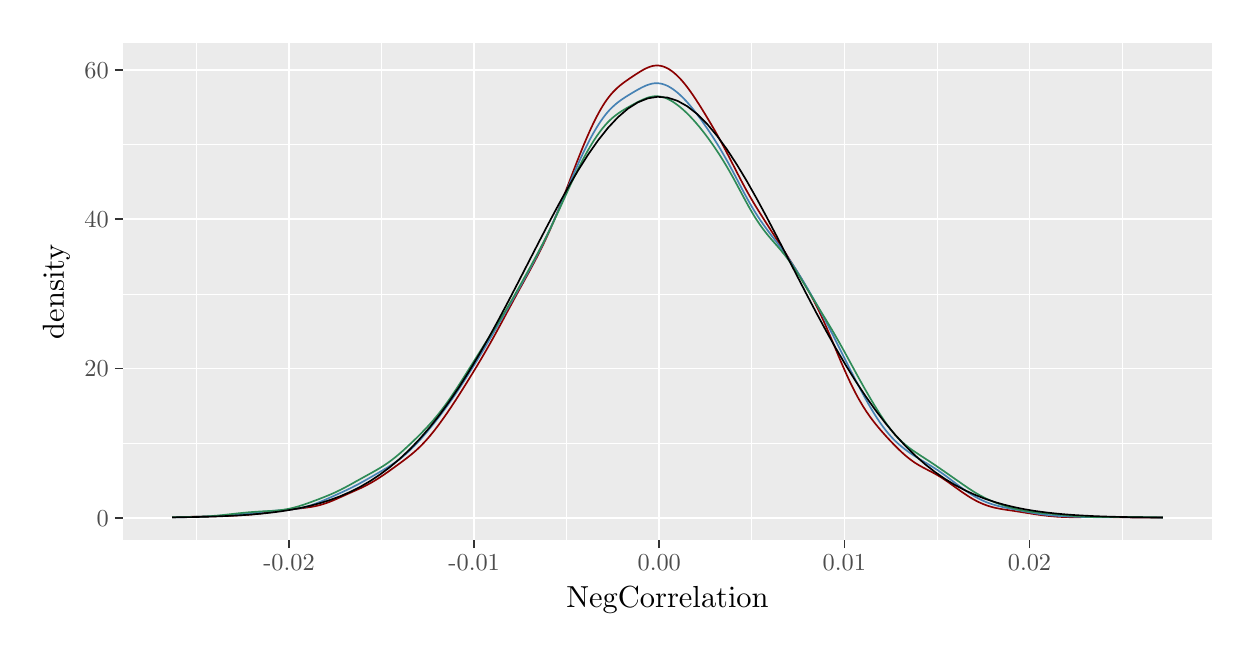
\begin{tikzpicture}[x=1pt,y=1pt]
\definecolor{fillColor}{RGB}{255,255,255}
\path[use as bounding box,fill=fillColor,fill opacity=0.00] (0,0) rectangle (433.62,216.81);
\begin{scope}
\path[clip] (  0.00,  0.00) rectangle (433.62,216.81);
\definecolor{drawColor}{RGB}{255,255,255}
\definecolor{fillColor}{RGB}{255,255,255}

\path[draw=drawColor,line width= 0.6pt,line join=round,line cap=round,fill=fillColor] (  0.00,  0.00) rectangle (433.62,216.81);
\end{scope}
\begin{scope}
\path[clip] ( 34.27, 31.53) rectangle (428.12,211.31);
\definecolor{fillColor}{gray}{0.92}

\path[fill=fillColor] ( 34.27, 31.53) rectangle (428.12,211.31);
\definecolor{drawColor}{RGB}{255,255,255}

\path[draw=drawColor,line width= 0.3pt,line join=round] ( 34.27, 66.67) --
	(428.12, 66.67);

\path[draw=drawColor,line width= 0.3pt,line join=round] ( 34.27,120.60) --
	(428.12,120.60);

\path[draw=drawColor,line width= 0.3pt,line join=round] ( 34.27,174.54) --
	(428.12,174.54);

\path[draw=drawColor,line width= 0.3pt,line join=round] ( 61.01, 31.53) --
	( 61.01,211.31);

\path[draw=drawColor,line width= 0.3pt,line join=round] (127.90, 31.53) --
	(127.90,211.31);

\path[draw=drawColor,line width= 0.3pt,line join=round] (194.78, 31.53) --
	(194.78,211.31);

\path[draw=drawColor,line width= 0.3pt,line join=round] (261.67, 31.53) --
	(261.67,211.31);

\path[draw=drawColor,line width= 0.3pt,line join=round] (328.56, 31.53) --
	(328.56,211.31);

\path[draw=drawColor,line width= 0.3pt,line join=round] (395.45, 31.53) --
	(395.45,211.31);

\path[draw=drawColor,line width= 0.6pt,line join=round] ( 34.27, 39.70) --
	(428.12, 39.70);

\path[draw=drawColor,line width= 0.6pt,line join=round] ( 34.27, 93.64) --
	(428.12, 93.64);

\path[draw=drawColor,line width= 0.6pt,line join=round] ( 34.27,147.57) --
	(428.12,147.57);

\path[draw=drawColor,line width= 0.6pt,line join=round] ( 34.27,201.50) --
	(428.12,201.50);

\path[draw=drawColor,line width= 0.6pt,line join=round] ( 94.45, 31.53) --
	( 94.45,211.31);

\path[draw=drawColor,line width= 0.6pt,line join=round] (161.34, 31.53) --
	(161.34,211.31);

\path[draw=drawColor,line width= 0.6pt,line join=round] (228.23, 31.53) --
	(228.23,211.31);

\path[draw=drawColor,line width= 0.6pt,line join=round] (295.12, 31.53) --
	(295.12,211.31);

\path[draw=drawColor,line width= 0.6pt,line join=round] (362.01, 31.53) --
	(362.01,211.31);
\definecolor{drawColor}{RGB}{139,0,0}

\path[draw=drawColor,line width= 0.6pt,line join=round] ( 52.17, 39.90) --
	( 52.87, 39.92) --
	( 53.57, 39.93) --
	( 54.27, 39.95) --
	( 54.97, 39.97) --
	( 55.67, 39.98) --
	( 56.37, 40.00) --
	( 57.07, 40.01) --
	( 57.78, 40.03) --
	( 58.48, 40.04) --
	( 59.18, 40.06) --
	( 59.88, 40.07) --
	( 60.58, 40.09) --
	( 61.28, 40.11) --
	( 61.98, 40.12) --
	( 62.68, 40.14) --
	( 63.38, 40.15) --
	( 64.08, 40.17) --
	( 64.78, 40.19) --
	( 65.48, 40.20) --
	( 66.18, 40.22) --
	( 66.88, 40.24) --
	( 67.59, 40.26) --
	( 68.29, 40.28) --
	( 68.99, 40.31) --
	( 69.69, 40.33) --
	( 70.39, 40.35) --
	( 71.09, 40.38) --
	( 71.79, 40.40) --
	( 72.49, 40.43) --
	( 73.19, 40.46) --
	( 73.89, 40.49) --
	( 74.59, 40.52) --
	( 75.29, 40.55) --
	( 75.99, 40.58) --
	( 76.69, 40.62) --
	( 77.39, 40.66) --
	( 78.10, 40.70) --
	( 78.80, 40.75) --
	( 79.50, 40.80) --
	( 80.20, 40.85) --
	( 80.90, 40.91) --
	( 81.60, 40.98) --
	( 82.30, 41.05) --
	( 83.00, 41.12) --
	( 83.70, 41.20) --
	( 84.40, 41.29) --
	( 85.10, 41.38) --
	( 85.80, 41.47) --
	( 86.50, 41.57) --
	( 87.20, 41.67) --
	( 87.90, 41.77) --
	( 88.61, 41.87) --
	( 89.31, 41.97) --
	( 90.01, 42.07) --
	( 90.71, 42.17) --
	( 91.41, 42.27) --
	( 92.11, 42.37) --
	( 92.81, 42.46) --
	( 93.51, 42.55) --
	( 94.21, 42.64) --
	( 94.91, 42.72) --
	( 95.61, 42.80) --
	( 96.31, 42.88) --
	( 97.01, 42.96) --
	( 97.71, 43.03) --
	( 98.42, 43.11) --
	( 99.12, 43.19) --
	( 99.82, 43.27) --
	(100.52, 43.35) --
	(101.22, 43.45) --
	(101.92, 43.55) --
	(102.62, 43.66) --
	(103.32, 43.79) --
	(104.02, 43.93) --
	(104.72, 44.09) --
	(105.42, 44.26) --
	(106.12, 44.45) --
	(106.82, 44.67) --
	(107.52, 44.89) --
	(108.22, 45.14) --
	(108.93, 45.41) --
	(109.63, 45.68) --
	(110.33, 45.97) --
	(111.03, 46.27) --
	(111.73, 46.57) --
	(112.43, 46.89) --
	(113.13, 47.20) --
	(113.83, 47.51) --
	(114.53, 47.83) --
	(115.23, 48.14) --
	(115.93, 48.45) --
	(116.63, 48.77) --
	(117.33, 49.08) --
	(118.03, 49.39) --
	(118.73, 49.70) --
	(119.44, 50.02) --
	(120.14, 50.34) --
	(120.84, 50.67) --
	(121.54, 51.01) --
	(122.24, 51.36) --
	(122.94, 51.73) --
	(123.64, 52.11) --
	(124.34, 52.50) --
	(125.04, 52.91) --
	(125.74, 53.33) --
	(126.44, 53.77) --
	(127.14, 54.22) --
	(127.84, 54.69) --
	(128.54, 55.16) --
	(129.24, 55.64) --
	(129.95, 56.13) --
	(130.65, 56.63) --
	(131.35, 57.13) --
	(132.05, 57.63) --
	(132.75, 58.14) --
	(133.45, 58.65) --
	(134.15, 59.16) --
	(134.85, 59.67) --
	(135.55, 60.19) --
	(136.25, 60.72) --
	(136.95, 61.25) --
	(137.65, 61.80) --
	(138.35, 62.36) --
	(139.05, 62.94) --
	(139.76, 63.54) --
	(140.46, 64.16) --
	(141.16, 64.81) --
	(141.86, 65.49) --
	(142.56, 66.19) --
	(143.26, 66.92) --
	(143.96, 67.68) --
	(144.66, 68.47) --
	(145.36, 69.29) --
	(146.06, 70.14) --
	(146.76, 71.01) --
	(147.46, 71.91) --
	(148.16, 72.83) --
	(148.86, 73.77) --
	(149.56, 74.74) --
	(150.27, 75.72) --
	(150.97, 76.71) --
	(151.67, 77.73) --
	(152.37, 78.76) --
	(153.07, 79.80) --
	(153.77, 80.86) --
	(154.47, 81.93) --
	(155.17, 83.01) --
	(155.87, 84.10) --
	(156.57, 85.21) --
	(157.27, 86.32) --
	(157.97, 87.44) --
	(158.67, 88.56) --
	(159.37, 89.70) --
	(160.07, 90.84) --
	(160.78, 91.98) --
	(161.48, 93.14) --
	(162.18, 94.29) --
	(162.88, 95.46) --
	(163.58, 96.63) --
	(164.28, 97.82) --
	(164.98, 99.02) --
	(165.68,100.22) --
	(166.38,101.45) --
	(167.08,102.68) --
	(167.78,103.93) --
	(168.48,105.19) --
	(169.18,106.46) --
	(169.88,107.75) --
	(170.59,109.05) --
	(171.29,110.35) --
	(171.99,111.66) --
	(172.69,112.97) --
	(173.39,114.28) --
	(174.09,115.58) --
	(174.79,116.88) --
	(175.49,118.18) --
	(176.19,119.47) --
	(176.89,120.76) --
	(177.59,122.04) --
	(178.29,123.31) --
	(178.99,124.58) --
	(179.69,125.86) --
	(180.39,127.13) --
	(181.10,128.42) --
	(181.80,129.71) --
	(182.50,131.02) --
	(183.20,132.34) --
	(183.90,133.68) --
	(184.60,135.05) --
	(185.30,136.44) --
	(186.00,137.86) --
	(186.70,139.31) --
	(187.40,140.80) --
	(188.10,142.33) --
	(188.80,143.90) --
	(189.50,145.51) --
	(190.20,147.15) --
	(190.90,148.83) --
	(191.61,150.55) --
	(192.31,152.30) --
	(193.01,154.08) --
	(193.71,155.89) --
	(194.41,157.71) --
	(195.11,159.54) --
	(195.81,161.38) --
	(196.51,163.22) --
	(197.21,165.05) --
	(197.91,166.86) --
	(198.61,168.66) --
	(199.31,170.44) --
	(200.01,172.18) --
	(200.71,173.90) --
	(201.42,175.58) --
	(202.12,177.22) --
	(202.82,178.82) --
	(203.52,180.37) --
	(204.22,181.86) --
	(204.92,183.30) --
	(205.62,184.67) --
	(206.32,185.99) --
	(207.02,187.24) --
	(207.72,188.42) --
	(208.42,189.53) --
	(209.12,190.56) --
	(209.82,191.51) --
	(210.52,192.39) --
	(211.22,193.21) --
	(211.93,193.96) --
	(212.63,194.66) --
	(213.33,195.30) --
	(214.03,195.90) --
	(214.73,196.46) --
	(215.43,196.98) --
	(216.13,197.49) --
	(216.83,197.98) --
	(217.53,198.46) --
	(218.23,198.93) --
	(218.93,199.40) --
	(219.63,199.86) --
	(220.33,200.31) --
	(221.03,200.75) --
	(221.73,201.18) --
	(222.44,201.58) --
	(223.14,201.95) --
	(223.84,202.28) --
	(224.54,202.57) --
	(225.24,202.81) --
	(225.94,202.99) --
	(226.64,203.10) --
	(227.34,203.14) --
	(228.04,203.11) --
	(228.74,203.01) --
	(229.44,202.84) --
	(230.14,202.60) --
	(230.84,202.30) --
	(231.54,201.92) --
	(232.24,201.47) --
	(232.95,200.97) --
	(233.65,200.41) --
	(234.35,199.79) --
	(235.05,199.12) --
	(235.75,198.40) --
	(236.45,197.63) --
	(237.15,196.81) --
	(237.85,195.94) --
	(238.55,195.02) --
	(239.25,194.07) --
	(239.95,193.08) --
	(240.65,192.05) --
	(241.35,191.00) --
	(242.05,189.92) --
	(242.76,188.82) --
	(243.46,187.71) --
	(244.16,186.57) --
	(244.86,185.43) --
	(245.56,184.27) --
	(246.26,183.10) --
	(246.96,181.92) --
	(247.66,180.72) --
	(248.36,179.51) --
	(249.06,178.27) --
	(249.76,177.02) --
	(250.46,175.74) --
	(251.16,174.44) --
	(251.86,173.13) --
	(252.56,171.79) --
	(253.27,170.44) --
	(253.97,169.07) --
	(254.67,167.70) --
	(255.37,166.33) --
	(256.07,164.96) --
	(256.77,163.60) --
	(257.47,162.25) --
	(258.17,160.92) --
	(258.87,159.61) --
	(259.57,158.32) --
	(260.27,157.07) --
	(260.97,155.84) --
	(261.67,154.63) --
	(262.37,153.44) --
	(263.07,152.28) --
	(263.78,151.14) --
	(264.48,150.01) --
	(265.18,148.89) --
	(265.88,147.79) --
	(266.58,146.69) --
	(267.28,145.60) --
	(267.98,144.51) --
	(268.68,143.42) --
	(269.38,142.33) --
	(270.08,141.23) --
	(270.78,140.14) --
	(271.48,139.04) --
	(272.18,137.94) --
	(272.88,136.83) --
	(273.59,135.73) --
	(274.29,134.62) --
	(274.99,133.51) --
	(275.69,132.39) --
	(276.39,131.28) --
	(277.09,130.15) --
	(277.79,129.03) --
	(278.49,127.89) --
	(279.19,126.74) --
	(279.89,125.58) --
	(280.59,124.40) --
	(281.29,123.20) --
	(281.99,121.98) --
	(282.69,120.72) --
	(283.39,119.42) --
	(284.10,118.09) --
	(284.80,116.72) --
	(285.50,115.31) --
	(286.20,113.86) --
	(286.90,112.37) --
	(287.60,110.84) --
	(288.30,109.26) --
	(289.00,107.66) --
	(289.70,106.03) --
	(290.40,104.38) --
	(291.10,102.71) --
	(291.80,101.04) --
	(292.50, 99.36) --
	(293.20, 97.69) --
	(293.90, 96.04) --
	(294.61, 94.42) --
	(295.31, 92.82) --
	(296.01, 91.25) --
	(296.71, 89.73) --
	(297.41, 88.24) --
	(298.11, 86.81) --
	(298.81, 85.42) --
	(299.51, 84.09) --
	(300.21, 82.81) --
	(300.91, 81.59) --
	(301.61, 80.41) --
	(302.31, 79.28) --
	(303.01, 78.20) --
	(303.71, 77.17) --
	(304.41, 76.18) --
	(305.12, 75.23) --
	(305.82, 74.31) --
	(306.52, 73.43) --
	(307.22, 72.58) --
	(307.92, 71.74) --
	(308.62, 70.93) --
	(309.32, 70.14) --
	(310.02, 69.36) --
	(310.72, 68.59) --
	(311.42, 67.84) --
	(312.12, 67.10) --
	(312.82, 66.37) --
	(313.52, 65.65) --
	(314.22, 64.95) --
	(314.93, 64.26) --
	(315.63, 63.60) --
	(316.33, 62.95) --
	(317.03, 62.33) --
	(317.73, 61.74) --
	(318.43, 61.18) --
	(319.13, 60.64) --
	(319.83, 60.13) --
	(320.53, 59.65) --
	(321.23, 59.20) --
	(321.93, 58.78) --
	(322.63, 58.37) --
	(323.33, 57.99) --
	(324.03, 57.61) --
	(324.73, 57.25) --
	(325.44, 56.89) --
	(326.14, 56.53) --
	(326.84, 56.16) --
	(327.54, 55.78) --
	(328.24, 55.39) --
	(328.94, 54.99) --
	(329.64, 54.57) --
	(330.34, 54.13) --
	(331.04, 53.67) --
	(331.74, 53.21) --
	(332.44, 52.72) --
	(333.14, 52.23) --
	(333.84, 51.72) --
	(334.54, 51.22) --
	(335.24, 50.71) --
	(335.95, 50.20) --
	(336.65, 49.70) --
	(337.35, 49.20) --
	(338.05, 48.71) --
	(338.75, 48.24) --
	(339.45, 47.78) --
	(340.15, 47.33) --
	(340.85, 46.90) --
	(341.55, 46.49) --
	(342.25, 46.10) --
	(342.95, 45.73) --
	(343.65, 45.38) --
	(344.35, 45.06) --
	(345.05, 44.76) --
	(345.76, 44.48) --
	(346.46, 44.22) --
	(347.16, 43.98) --
	(347.86, 43.77) --
	(348.56, 43.57) --
	(349.26, 43.39) --
	(349.96, 43.23) --
	(350.66, 43.09) --
	(351.36, 42.95) --
	(352.06, 42.83) --
	(352.76, 42.72) --
	(353.46, 42.61) --
	(354.16, 42.50) --
	(354.86, 42.40) --
	(355.56, 42.30) --
	(356.27, 42.20) --
	(356.97, 42.09) --
	(357.67, 41.99) --
	(358.37, 41.88) --
	(359.07, 41.77) --
	(359.77, 41.66) --
	(360.47, 41.55) --
	(361.17, 41.44) --
	(361.87, 41.33) --
	(362.57, 41.22) --
	(363.27, 41.11) --
	(363.97, 41.00) --
	(364.67, 40.90) --
	(365.37, 40.80) --
	(366.07, 40.70) --
	(366.78, 40.61) --
	(367.48, 40.53) --
	(368.18, 40.45) --
	(368.88, 40.37) --
	(369.58, 40.30) --
	(370.28, 40.23) --
	(370.98, 40.18) --
	(371.68, 40.12) --
	(372.38, 40.08) --
	(373.08, 40.04) --
	(373.78, 40.00) --
	(374.48, 39.98) --
	(375.18, 39.95) --
	(375.88, 39.94) --
	(376.58, 39.92) --
	(377.29, 39.92) --
	(377.99, 39.91) --
	(378.69, 39.92) --
	(379.39, 39.92) --
	(380.09, 39.92) --
	(380.79, 39.93) --
	(381.49, 39.94) --
	(382.19, 39.95) --
	(382.89, 39.95) --
	(383.59, 39.96) --
	(384.29, 39.97) --
	(384.99, 39.97) --
	(385.69, 39.97) --
	(386.39, 39.97) --
	(387.10, 39.97) --
	(387.80, 39.97) --
	(388.50, 39.97) --
	(389.20, 39.96) --
	(389.90, 39.95) --
	(390.60, 39.94) --
	(391.30, 39.94) --
	(392.00, 39.93) --
	(392.70, 39.92) --
	(393.40, 39.91) --
	(394.10, 39.90) --
	(394.80, 39.89) --
	(395.50, 39.87) --
	(396.20, 39.86) --
	(396.90, 39.86) --
	(397.61, 39.85) --
	(398.31, 39.84) --
	(399.01, 39.83) --
	(399.71, 39.83) --
	(400.41, 39.82) --
	(401.11, 39.82) --
	(401.81, 39.81) --
	(402.51, 39.81) --
	(403.21, 39.81) --
	(403.91, 39.81) --
	(404.61, 39.81) --
	(405.31, 39.81) --
	(406.01, 39.82) --
	(406.71, 39.82) --
	(407.41, 39.82) --
	(408.12, 39.82) --
	(408.82, 39.82) --
	(409.52, 39.82) --
	(410.22, 39.82);
\definecolor{drawColor}{RGB}{70,130,180}

\path[draw=drawColor,line width= 0.6pt,line join=round] ( 52.17, 39.85) --
	( 52.87, 39.86) --
	( 53.57, 39.87) --
	( 54.27, 39.88) --
	( 54.97, 39.90) --
	( 55.67, 39.91) --
	( 56.37, 39.92) --
	( 57.07, 39.94) --
	( 57.78, 39.95) --
	( 58.48, 39.97) --
	( 59.18, 39.99) --
	( 59.88, 40.02) --
	( 60.58, 40.04) --
	( 61.28, 40.07) --
	( 61.98, 40.09) --
	( 62.68, 40.12) --
	( 63.38, 40.15) --
	( 64.08, 40.18) --
	( 64.78, 40.21) --
	( 65.48, 40.25) --
	( 66.18, 40.28) --
	( 66.88, 40.31) --
	( 67.59, 40.35) --
	( 68.29, 40.38) --
	( 68.99, 40.42) --
	( 69.69, 40.46) --
	( 70.39, 40.50) --
	( 71.09, 40.54) --
	( 71.79, 40.58) --
	( 72.49, 40.63) --
	( 73.19, 40.67) --
	( 73.89, 40.73) --
	( 74.59, 40.78) --
	( 75.29, 40.84) --
	( 75.99, 40.90) --
	( 76.69, 40.97) --
	( 77.39, 41.04) --
	( 78.10, 41.11) --
	( 78.80, 41.18) --
	( 79.50, 41.26) --
	( 80.20, 41.34) --
	( 80.90, 41.42) --
	( 81.60, 41.50) --
	( 82.30, 41.58) --
	( 83.00, 41.66) --
	( 83.70, 41.74) --
	( 84.40, 41.81) --
	( 85.10, 41.89) --
	( 85.80, 41.96) --
	( 86.50, 42.03) --
	( 87.20, 42.09) --
	( 87.90, 42.15) --
	( 88.61, 42.21) --
	( 89.31, 42.26) --
	( 90.01, 42.31) --
	( 90.71, 42.36) --
	( 91.41, 42.41) --
	( 92.11, 42.46) --
	( 92.81, 42.51) --
	( 93.51, 42.57) --
	( 94.21, 42.63) --
	( 94.91, 42.70) --
	( 95.61, 42.77) --
	( 96.31, 42.86) --
	( 97.01, 42.96) --
	( 97.71, 43.08) --
	( 98.42, 43.21) --
	( 99.12, 43.35) --
	( 99.82, 43.51) --
	(100.52, 43.69) --
	(101.22, 43.89) --
	(101.92, 44.10) --
	(102.62, 44.33) --
	(103.32, 44.57) --
	(104.02, 44.82) --
	(104.72, 45.09) --
	(105.42, 45.37) --
	(106.12, 45.65) --
	(106.82, 45.95) --
	(107.52, 46.25) --
	(108.22, 46.55) --
	(108.93, 46.86) --
	(109.63, 47.17) --
	(110.33, 47.48) --
	(111.03, 47.80) --
	(111.73, 48.11) --
	(112.43, 48.43) --
	(113.13, 48.75) --
	(113.83, 49.07) --
	(114.53, 49.39) --
	(115.23, 49.72) --
	(115.93, 50.05) --
	(116.63, 50.39) --
	(117.33, 50.74) --
	(118.03, 51.10) --
	(118.73, 51.46) --
	(119.44, 51.83) --
	(120.14, 52.21) --
	(120.84, 52.60) --
	(121.54, 52.99) --
	(122.24, 53.38) --
	(122.94, 53.78) --
	(123.64, 54.18) --
	(124.34, 54.58) --
	(125.04, 54.98) --
	(125.74, 55.38) --
	(126.44, 55.79) --
	(127.14, 56.19) --
	(127.84, 56.60) --
	(128.54, 57.02) --
	(129.24, 57.44) --
	(129.95, 57.86) --
	(130.65, 58.30) --
	(131.35, 58.75) --
	(132.05, 59.21) --
	(132.75, 59.69) --
	(133.45, 60.18) --
	(134.15, 60.70) --
	(134.85, 61.25) --
	(135.55, 61.81) --
	(136.25, 62.40) --
	(136.95, 63.01) --
	(137.65, 63.64) --
	(138.35, 64.30) --
	(139.05, 64.99) --
	(139.76, 65.69) --
	(140.46, 66.42) --
	(141.16, 67.17) --
	(141.86, 67.94) --
	(142.56, 68.73) --
	(143.26, 69.53) --
	(143.96, 70.35) --
	(144.66, 71.19) --
	(145.36, 72.04) --
	(146.06, 72.90) --
	(146.76, 73.77) --
	(147.46, 74.66) --
	(148.16, 75.56) --
	(148.86, 76.47) --
	(149.56, 77.39) --
	(150.27, 78.33) --
	(150.97, 79.28) --
	(151.67, 80.24) --
	(152.37, 81.22) --
	(153.07, 82.21) --
	(153.77, 83.22) --
	(154.47, 84.24) --
	(155.17, 85.28) --
	(155.87, 86.33) --
	(156.57, 87.39) --
	(157.27, 88.47) --
	(157.97, 89.55) --
	(158.67, 90.65) --
	(159.37, 91.75) --
	(160.07, 92.87) --
	(160.78, 93.99) --
	(161.48, 95.12) --
	(162.18, 96.25) --
	(162.88, 97.40) --
	(163.58, 98.55) --
	(164.28, 99.71) --
	(164.98,100.88) --
	(165.68,102.05) --
	(166.38,103.23) --
	(167.08,104.42) --
	(167.78,105.61) --
	(168.48,106.81) --
	(169.18,108.01) --
	(169.88,109.21) --
	(170.59,110.42) --
	(171.29,111.63) --
	(171.99,112.84) --
	(172.69,114.05) --
	(173.39,115.26) --
	(174.09,116.48) --
	(174.79,117.69) --
	(175.49,118.91) --
	(176.19,120.14) --
	(176.89,121.37) --
	(177.59,122.61) --
	(178.29,123.86) --
	(178.99,125.11) --
	(179.69,126.37) --
	(180.39,127.64) --
	(181.10,128.93) --
	(181.80,130.22) --
	(182.50,131.53) --
	(183.20,132.85) --
	(183.90,134.19) --
	(184.60,135.55) --
	(185.30,136.93) --
	(186.00,138.33) --
	(186.70,139.75) --
	(187.40,141.20) --
	(188.10,142.68) --
	(188.80,144.19) --
	(189.50,145.73) --
	(190.20,147.29) --
	(190.90,148.88) --
	(191.61,150.49) --
	(192.31,152.13) --
	(193.01,153.78) --
	(193.71,155.44) --
	(194.41,157.10) --
	(195.11,158.77) --
	(195.81,160.43) --
	(196.51,162.09) --
	(197.21,163.72) --
	(197.91,165.34) --
	(198.61,166.93) --
	(199.31,168.49) --
	(200.01,170.02) --
	(200.71,171.51) --
	(201.42,172.97) --
	(202.12,174.38) --
	(202.82,175.75) --
	(203.52,177.08) --
	(204.22,178.36) --
	(204.92,179.58) --
	(205.62,180.75) --
	(206.32,181.87) --
	(207.02,182.93) --
	(207.72,183.93) --
	(208.42,184.87) --
	(209.12,185.76) --
	(209.82,186.58) --
	(210.52,187.34) --
	(211.22,188.04) --
	(211.93,188.69) --
	(212.63,189.30) --
	(213.33,189.86) --
	(214.03,190.39) --
	(214.73,190.89) --
	(215.43,191.36) --
	(216.13,191.81) --
	(216.83,192.25) --
	(217.53,192.68) --
	(218.23,193.10) --
	(218.93,193.52) --
	(219.63,193.93) --
	(220.33,194.33) --
	(221.03,194.72) --
	(221.73,195.09) --
	(222.44,195.44) --
	(223.14,195.76) --
	(223.84,196.05) --
	(224.54,196.29) --
	(225.24,196.49) --
	(225.94,196.64) --
	(226.64,196.72) --
	(227.34,196.74) --
	(228.04,196.70) --
	(228.74,196.60) --
	(229.44,196.44) --
	(230.14,196.21) --
	(230.84,195.93) --
	(231.54,195.59) --
	(232.24,195.18) --
	(232.95,194.73) --
	(233.65,194.24) --
	(234.35,193.69) --
	(235.05,193.11) --
	(235.75,192.49) --
	(236.45,191.82) --
	(237.15,191.12) --
	(237.85,190.38) --
	(238.55,189.61) --
	(239.25,188.80) --
	(239.95,187.96) --
	(240.65,187.09) --
	(241.35,186.20) --
	(242.05,185.28) --
	(242.76,184.33) --
	(243.46,183.37) --
	(244.16,182.38) --
	(244.86,181.37) --
	(245.56,180.35) --
	(246.26,179.31) --
	(246.96,178.25) --
	(247.66,177.18) --
	(248.36,176.08) --
	(249.06,174.96) --
	(249.76,173.82) --
	(250.46,172.65) --
	(251.16,171.45) --
	(251.86,170.23) --
	(252.56,168.99) --
	(253.27,167.72) --
	(253.97,166.42) --
	(254.67,165.11) --
	(255.37,163.78) --
	(256.07,162.45) --
	(256.77,161.11) --
	(257.47,159.77) --
	(258.17,158.44) --
	(258.87,157.12) --
	(259.57,155.83) --
	(260.27,154.56) --
	(260.97,153.32) --
	(261.67,152.11) --
	(262.37,150.94) --
	(263.07,149.80) --
	(263.78,148.70) --
	(264.48,147.64) --
	(265.18,146.61) --
	(265.88,145.61) --
	(266.58,144.64) --
	(267.28,143.69) --
	(267.98,142.76) --
	(268.68,141.84) --
	(269.38,140.93) --
	(270.08,140.02) --
	(270.78,139.10) --
	(271.48,138.18) --
	(272.18,137.25) --
	(272.88,136.30) --
	(273.59,135.34) --
	(274.29,134.35) --
	(274.99,133.35) --
	(275.69,132.32) --
	(276.39,131.28) --
	(277.09,130.21) --
	(277.79,129.13) --
	(278.49,128.02) --
	(279.19,126.90) --
	(279.89,125.76) --
	(280.59,124.60) --
	(281.29,123.43) --
	(281.99,122.24) --
	(282.69,121.03) --
	(283.39,119.81) --
	(284.10,118.58) --
	(284.80,117.33) --
	(285.50,116.06) --
	(286.20,114.78) --
	(286.90,113.49) --
	(287.60,112.18) --
	(288.30,110.86) --
	(289.00,109.52) --
	(289.70,108.17) --
	(290.40,106.81) --
	(291.10,105.44) --
	(291.80,104.06) --
	(292.50,102.67) --
	(293.20,101.28) --
	(293.90, 99.88) --
	(294.61, 98.48) --
	(295.31, 97.07) --
	(296.01, 95.68) --
	(296.71, 94.28) --
	(297.41, 92.89) --
	(298.11, 91.51) --
	(298.81, 90.14) --
	(299.51, 88.79) --
	(300.21, 87.44) --
	(300.91, 86.11) --
	(301.61, 84.80) --
	(302.31, 83.51) --
	(303.01, 82.25) --
	(303.71, 81.00) --
	(304.41, 79.79) --
	(305.12, 78.61) --
	(305.82, 77.45) --
	(306.52, 76.34) --
	(307.22, 75.26) --
	(307.92, 74.22) --
	(308.62, 73.23) --
	(309.32, 72.28) --
	(310.02, 71.37) --
	(310.72, 70.50) --
	(311.42, 69.68) --
	(312.12, 68.89) --
	(312.82, 68.15) --
	(313.52, 67.45) --
	(314.22, 66.79) --
	(314.93, 66.15) --
	(315.63, 65.55) --
	(316.33, 64.98) --
	(317.03, 64.43) --
	(317.73, 63.91) --
	(318.43, 63.41) --
	(319.13, 62.92) --
	(319.83, 62.46) --
	(320.53, 62.00) --
	(321.23, 61.56) --
	(321.93, 61.13) --
	(322.63, 60.71) --
	(323.33, 60.29) --
	(324.03, 59.87) --
	(324.73, 59.46) --
	(325.44, 59.04) --
	(326.14, 58.61) --
	(326.84, 58.18) --
	(327.54, 57.74) --
	(328.24, 57.29) --
	(328.94, 56.83) --
	(329.64, 56.35) --
	(330.34, 55.86) --
	(331.04, 55.36) --
	(331.74, 54.85) --
	(332.44, 54.33) --
	(333.14, 53.81) --
	(333.84, 53.28) --
	(334.54, 52.74) --
	(335.24, 52.21) --
	(335.95, 51.68) --
	(336.65, 51.15) --
	(337.35, 50.63) --
	(338.05, 50.13) --
	(338.75, 49.63) --
	(339.45, 49.15) --
	(340.15, 48.68) --
	(340.85, 48.24) --
	(341.55, 47.81) --
	(342.25, 47.40) --
	(342.95, 47.01) --
	(343.65, 46.63) --
	(344.35, 46.28) --
	(345.05, 45.95) --
	(345.76, 45.64) --
	(346.46, 45.35) --
	(347.16, 45.08) --
	(347.86, 44.83) --
	(348.56, 44.60) --
	(349.26, 44.38) --
	(349.96, 44.18) --
	(350.66, 43.99) --
	(351.36, 43.82) --
	(352.06, 43.65) --
	(352.76, 43.49) --
	(353.46, 43.34) --
	(354.16, 43.20) --
	(354.86, 43.06) --
	(355.56, 42.92) --
	(356.27, 42.78) --
	(356.97, 42.65) --
	(357.67, 42.51) --
	(358.37, 42.38) --
	(359.07, 42.24) --
	(359.77, 42.11) --
	(360.47, 41.97) --
	(361.17, 41.84) --
	(361.87, 41.71) --
	(362.57, 41.58) --
	(363.27, 41.46) --
	(363.97, 41.34) --
	(364.67, 41.22) --
	(365.37, 41.11) --
	(366.07, 41.01) --
	(366.78, 40.92) --
	(367.48, 40.83) --
	(368.18, 40.75) --
	(368.88, 40.67) --
	(369.58, 40.60) --
	(370.28, 40.54) --
	(370.98, 40.48) --
	(371.68, 40.43) --
	(372.38, 40.38) --
	(373.08, 40.34) --
	(373.78, 40.30) --
	(374.48, 40.26) --
	(375.18, 40.22) --
	(375.88, 40.19) --
	(376.58, 40.16) --
	(377.29, 40.13) --
	(377.99, 40.11) --
	(378.69, 40.08) --
	(379.39, 40.06) --
	(380.09, 40.04) --
	(380.79, 40.01) --
	(381.49, 40.00) --
	(382.19, 39.98) --
	(382.89, 39.96) --
	(383.59, 39.95) --
	(384.29, 39.94) --
	(384.99, 39.93) --
	(385.69, 39.92) --
	(386.39, 39.92) --
	(387.10, 39.92) --
	(387.80, 39.92) --
	(388.50, 39.92) --
	(389.20, 39.92) --
	(389.90, 39.92) --
	(390.60, 39.92) --
	(391.30, 39.92) --
	(392.00, 39.93) --
	(392.70, 39.93) --
	(393.40, 39.93) --
	(394.10, 39.93) --
	(394.80, 39.93) --
	(395.50, 39.93) --
	(396.20, 39.92) --
	(396.90, 39.92) --
	(397.61, 39.92) --
	(398.31, 39.91) --
	(399.01, 39.91) --
	(399.71, 39.90) --
	(400.41, 39.90) --
	(401.11, 39.89) --
	(401.81, 39.89) --
	(402.51, 39.88) --
	(403.21, 39.87) --
	(403.91, 39.87) --
	(404.61, 39.86) --
	(405.31, 39.86) --
	(406.01, 39.86) --
	(406.71, 39.85) --
	(407.41, 39.85) --
	(408.12, 39.84) --
	(408.82, 39.83) --
	(409.52, 39.83) --
	(410.22, 39.82);
\definecolor{drawColor}{RGB}{46,139,87}

\path[draw=drawColor,line width= 0.6pt,line join=round] ( 52.17, 39.91) --
	( 52.87, 39.92) --
	( 53.57, 39.93) --
	( 54.27, 39.95) --
	( 54.97, 39.96) --
	( 55.67, 39.97) --
	( 56.37, 39.98) --
	( 57.07, 39.99) --
	( 57.78, 40.01) --
	( 58.48, 40.02) --
	( 59.18, 40.03) --
	( 59.88, 40.05) --
	( 60.58, 40.07) --
	( 61.28, 40.09) --
	( 61.98, 40.11) --
	( 62.68, 40.13) --
	( 63.38, 40.16) --
	( 64.08, 40.19) --
	( 64.78, 40.23) --
	( 65.48, 40.27) --
	( 66.18, 40.32) --
	( 66.88, 40.37) --
	( 67.59, 40.43) --
	( 68.29, 40.49) --
	( 68.99, 40.55) --
	( 69.69, 40.62) --
	( 70.39, 40.69) --
	( 71.09, 40.77) --
	( 71.79, 40.84) --
	( 72.49, 40.92) --
	( 73.19, 41.00) --
	( 73.89, 41.08) --
	( 74.59, 41.15) --
	( 75.29, 41.23) --
	( 75.99, 41.31) --
	( 76.69, 41.38) --
	( 77.39, 41.46) --
	( 78.10, 41.53) --
	( 78.80, 41.59) --
	( 79.50, 41.66) --
	( 80.20, 41.72) --
	( 80.90, 41.77) --
	( 81.60, 41.83) --
	( 82.30, 41.88) --
	( 83.00, 41.93) --
	( 83.70, 41.97) --
	( 84.40, 42.01) --
	( 85.10, 42.05) --
	( 85.80, 42.08) --
	( 86.50, 42.12) --
	( 87.20, 42.16) --
	( 87.90, 42.20) --
	( 88.61, 42.24) --
	( 89.31, 42.29) --
	( 90.01, 42.35) --
	( 90.71, 42.42) --
	( 91.41, 42.49) --
	( 92.11, 42.58) --
	( 92.81, 42.69) --
	( 93.51, 42.80) --
	( 94.21, 42.93) --
	( 94.91, 43.08) --
	( 95.61, 43.24) --
	( 96.31, 43.42) --
	( 97.01, 43.61) --
	( 97.71, 43.81) --
	( 98.42, 44.02) --
	( 99.12, 44.25) --
	( 99.82, 44.48) --
	(100.52, 44.72) --
	(101.22, 44.97) --
	(101.92, 45.22) --
	(102.62, 45.48) --
	(103.32, 45.74) --
	(104.02, 46.00) --
	(104.72, 46.26) --
	(105.42, 46.53) --
	(106.12, 46.80) --
	(106.82, 47.08) --
	(107.52, 47.36) --
	(108.22, 47.64) --
	(108.93, 47.93) --
	(109.63, 48.23) --
	(110.33, 48.54) --
	(111.03, 48.85) --
	(111.73, 49.18) --
	(112.43, 49.52) --
	(113.13, 49.86) --
	(113.83, 50.22) --
	(114.53, 50.59) --
	(115.23, 50.96) --
	(115.93, 51.34) --
	(116.63, 51.72) --
	(117.33, 52.11) --
	(118.03, 52.50) --
	(118.73, 52.90) --
	(119.44, 53.29) --
	(120.14, 53.68) --
	(120.84, 54.07) --
	(121.54, 54.45) --
	(122.24, 54.84) --
	(122.94, 55.23) --
	(123.64, 55.61) --
	(124.34, 56.00) --
	(125.04, 56.39) --
	(125.74, 56.79) --
	(126.44, 57.19) --
	(127.14, 57.61) --
	(127.84, 58.04) --
	(128.54, 58.48) --
	(129.24, 58.94) --
	(129.95, 59.42) --
	(130.65, 59.91) --
	(131.35, 60.43) --
	(132.05, 60.97) --
	(132.75, 61.52) --
	(133.45, 62.09) --
	(134.15, 62.68) --
	(134.85, 63.29) --
	(135.55, 63.90) --
	(136.25, 64.54) --
	(136.95, 65.18) --
	(137.65, 65.83) --
	(138.35, 66.49) --
	(139.05, 67.16) --
	(139.76, 67.83) --
	(140.46, 68.52) --
	(141.16, 69.21) --
	(141.86, 69.91) --
	(142.56, 70.62) --
	(143.26, 71.34) --
	(143.96, 72.08) --
	(144.66, 72.83) --
	(145.36, 73.60) --
	(146.06, 74.38) --
	(146.76, 75.19) --
	(147.46, 76.02) --
	(148.16, 76.88) --
	(148.86, 77.76) --
	(149.56, 78.66) --
	(150.27, 79.59) --
	(150.97, 80.54) --
	(151.67, 81.51) --
	(152.37, 82.51) --
	(153.07, 83.53) --
	(153.77, 84.56) --
	(154.47, 85.62) --
	(155.17, 86.69) --
	(155.87, 87.77) --
	(156.57, 88.86) --
	(157.27, 89.96) --
	(157.97, 91.07) --
	(158.67, 92.18) --
	(159.37, 93.30) --
	(160.07, 94.41) --
	(160.78, 95.53) --
	(161.48, 96.65) --
	(162.18, 97.77) --
	(162.88, 98.88) --
	(163.58, 99.99) --
	(164.28,101.10) --
	(164.98,102.21) --
	(165.68,103.31) --
	(166.38,104.42) --
	(167.08,105.52) --
	(167.78,106.63) --
	(168.48,107.74) --
	(169.18,108.86) --
	(169.88,109.99) --
	(170.59,111.12) --
	(171.29,112.26) --
	(171.99,113.42) --
	(172.69,114.58) --
	(173.39,115.77) --
	(174.09,116.96) --
	(174.79,118.16) --
	(175.49,119.38) --
	(176.19,120.61) --
	(176.89,121.85) --
	(177.59,123.09) --
	(178.29,124.35) --
	(178.99,125.61) --
	(179.69,126.87) --
	(180.39,128.14) --
	(181.10,129.41) --
	(181.80,130.69) --
	(182.50,131.97) --
	(183.20,133.26) --
	(183.90,134.56) --
	(184.60,135.87) --
	(185.30,137.19) --
	(186.00,138.53) --
	(186.70,139.89) --
	(187.40,141.27) --
	(188.10,142.68) --
	(188.80,144.11) --
	(189.50,145.56) --
	(190.20,147.04) --
	(190.90,148.54) --
	(191.61,150.06) --
	(192.31,151.59) --
	(193.01,153.13) --
	(193.71,154.68) --
	(194.41,156.23) --
	(195.11,157.77) --
	(195.81,159.30) --
	(196.51,160.81) --
	(197.21,162.30) --
	(197.91,163.77) --
	(198.61,165.21) --
	(199.31,166.62) --
	(200.01,167.99) --
	(200.71,169.32) --
	(201.42,170.62) --
	(202.12,171.89) --
	(202.82,173.11) --
	(203.52,174.30) --
	(204.22,175.44) --
	(204.92,176.54) --
	(205.62,177.58) --
	(206.32,178.58) --
	(207.02,179.53) --
	(207.72,180.43) --
	(208.42,181.28) --
	(209.12,182.07) --
	(209.82,182.82) --
	(210.52,183.50) --
	(211.22,184.13) --
	(211.93,184.72) --
	(212.63,185.27) --
	(213.33,185.78) --
	(214.03,186.26) --
	(214.73,186.72) --
	(215.43,187.15) --
	(216.13,187.56) --
	(216.83,187.97) --
	(217.53,188.36) --
	(218.23,188.75) --
	(218.93,189.13) --
	(219.63,189.51) --
	(220.33,189.88) --
	(221.03,190.23) --
	(221.73,190.57) --
	(222.44,190.89) --
	(223.14,191.18) --
	(223.84,191.44) --
	(224.54,191.66) --
	(225.24,191.83) --
	(225.94,191.96) --
	(226.64,192.03) --
	(227.34,192.04) --
	(228.04,191.99) --
	(228.74,191.89) --
	(229.44,191.73) --
	(230.14,191.51) --
	(230.84,191.24) --
	(231.54,190.92) --
	(232.24,190.55) --
	(232.95,190.14) --
	(233.65,189.68) --
	(234.35,189.19) --
	(235.05,188.67) --
	(235.75,188.11) --
	(236.45,187.52) --
	(237.15,186.90) --
	(237.85,186.25) --
	(238.55,185.56) --
	(239.25,184.86) --
	(239.95,184.12) --
	(240.65,183.36) --
	(241.35,182.57) --
	(242.05,181.75) --
	(242.76,180.91) --
	(243.46,180.04) --
	(244.16,179.15) --
	(244.86,178.24) --
	(245.56,177.30) --
	(246.26,176.35) --
	(246.96,175.37) --
	(247.66,174.38) --
	(248.36,173.36) --
	(249.06,172.31) --
	(249.76,171.25) --
	(250.46,170.15) --
	(251.16,169.04) --
	(251.86,167.89) --
	(252.56,166.72) --
	(253.27,165.51) --
	(253.97,164.28) --
	(254.67,163.03) --
	(255.37,161.76) --
	(256.07,160.47) --
	(256.77,159.16) --
	(257.47,157.85) --
	(258.17,156.54) --
	(258.87,155.23) --
	(259.57,153.94) --
	(260.27,152.67) --
	(260.97,151.42) --
	(261.67,150.21) --
	(262.37,149.03) --
	(263.07,147.90) --
	(263.78,146.82) --
	(264.48,145.78) --
	(265.18,144.79) --
	(265.88,143.84) --
	(266.58,142.93) --
	(267.28,142.05) --
	(267.98,141.21) --
	(268.68,140.39) --
	(269.38,139.59) --
	(270.08,138.79) --
	(270.78,137.99) --
	(271.48,137.18) --
	(272.18,136.35) --
	(272.88,135.50) --
	(273.59,134.63) --
	(274.29,133.72) --
	(274.99,132.77) --
	(275.69,131.79) --
	(276.39,130.78) --
	(277.09,129.74) --
	(277.79,128.67) --
	(278.49,127.58) --
	(279.19,126.46) --
	(279.89,125.32) --
	(280.59,124.18) --
	(281.29,123.02) --
	(281.99,121.87) --
	(282.69,120.71) --
	(283.39,119.55) --
	(284.10,118.40) --
	(284.80,117.25) --
	(285.50,116.10) --
	(286.20,114.96) --
	(286.90,113.81) --
	(287.60,112.67) --
	(288.30,111.52) --
	(289.00,110.36) --
	(289.70,109.20) --
	(290.40,108.02) --
	(291.10,106.83) --
	(291.80,105.62) --
	(292.50,104.40) --
	(293.20,103.17) --
	(293.90,101.92) --
	(294.61,100.66) --
	(295.31, 99.39) --
	(296.01, 98.11) --
	(296.71, 96.82) --
	(297.41, 95.53) --
	(298.11, 94.24) --
	(298.81, 92.96) --
	(299.51, 91.68) --
	(300.21, 90.40) --
	(300.91, 89.14) --
	(301.61, 87.89) --
	(302.31, 86.64) --
	(303.01, 85.42) --
	(303.71, 84.20) --
	(304.41, 83.00) --
	(305.12, 81.81) --
	(305.82, 80.64) --
	(306.52, 79.49) --
	(307.22, 78.37) --
	(307.92, 77.26) --
	(308.62, 76.18) --
	(309.32, 75.13) --
	(310.02, 74.12) --
	(310.72, 73.13) --
	(311.42, 72.19) --
	(312.12, 71.30) --
	(312.82, 70.44) --
	(313.52, 69.63) --
	(314.22, 68.86) --
	(314.93, 68.13) --
	(315.63, 67.44) --
	(316.33, 66.80) --
	(317.03, 66.20) --
	(317.73, 65.63) --
	(318.43, 65.08) --
	(319.13, 64.56) --
	(319.83, 64.06) --
	(320.53, 63.58) --
	(321.23, 63.11) --
	(321.93, 62.65) --
	(322.63, 62.19) --
	(323.33, 61.74) --
	(324.03, 61.28) --
	(324.73, 60.83) --
	(325.44, 60.37) --
	(326.14, 59.91) --
	(326.84, 59.44) --
	(327.54, 58.97) --
	(328.24, 58.50) --
	(328.94, 58.02) --
	(329.64, 57.54) --
	(330.34, 57.06) --
	(331.04, 56.58) --
	(331.74, 56.09) --
	(332.44, 55.60) --
	(333.14, 55.11) --
	(333.84, 54.62) --
	(334.54, 54.13) --
	(335.24, 53.64) --
	(335.95, 53.14) --
	(336.65, 52.65) --
	(337.35, 52.16) --
	(338.05, 51.68) --
	(338.75, 51.20) --
	(339.45, 50.72) --
	(340.15, 50.25) --
	(340.85, 49.80) --
	(341.55, 49.35) --
	(342.25, 48.91) --
	(342.95, 48.49) --
	(343.65, 48.09) --
	(344.35, 47.69) --
	(345.05, 47.32) --
	(345.76, 46.96) --
	(346.46, 46.61) --
	(347.16, 46.28) --
	(347.86, 45.97) --
	(348.56, 45.67) --
	(349.26, 45.38) --
	(349.96, 45.11) --
	(350.66, 44.84) --
	(351.36, 44.59) --
	(352.06, 44.35) --
	(352.76, 44.12) --
	(353.46, 43.90) --
	(354.16, 43.69) --
	(354.86, 43.48) --
	(355.56, 43.29) --
	(356.27, 43.11) --
	(356.97, 42.93) --
	(357.67, 42.77) --
	(358.37, 42.61) --
	(359.07, 42.47) --
	(359.77, 42.33) --
	(360.47, 42.21) --
	(361.17, 42.09) --
	(361.87, 41.98) --
	(362.57, 41.89) --
	(363.27, 41.79) --
	(363.97, 41.71) --
	(364.67, 41.63) --
	(365.37, 41.56) --
	(366.07, 41.49) --
	(366.78, 41.42) --
	(367.48, 41.35) --
	(368.18, 41.29) --
	(368.88, 41.22) --
	(369.58, 41.16) --
	(370.28, 41.10) --
	(370.98, 41.03) --
	(371.68, 40.97) --
	(372.38, 40.90) --
	(373.08, 40.83) --
	(373.78, 40.76) --
	(374.48, 40.70) --
	(375.18, 40.63) --
	(375.88, 40.56) --
	(376.58, 40.50) --
	(377.29, 40.44) --
	(377.99, 40.38) --
	(378.69, 40.32) --
	(379.39, 40.27) --
	(380.09, 40.22) --
	(380.79, 40.17) --
	(381.49, 40.13) --
	(382.19, 40.10) --
	(382.89, 40.06) --
	(383.59, 40.03) --
	(384.29, 40.01) --
	(384.99, 39.99) --
	(385.69, 39.97) --
	(386.39, 39.96) --
	(387.10, 39.95) --
	(387.80, 39.94) --
	(388.50, 39.94) --
	(389.20, 39.94) --
	(389.90, 39.94) --
	(390.60, 39.94) --
	(391.30, 39.94) --
	(392.00, 39.95) --
	(392.70, 39.95) --
	(393.40, 39.96) --
	(394.10, 39.97) --
	(394.80, 39.97) --
	(395.50, 39.98) --
	(396.20, 39.98) --
	(396.90, 39.99) --
	(397.61, 39.99) --
	(398.31, 39.99) --
	(399.01, 39.99) --
	(399.71, 39.99) --
	(400.41, 39.99) --
	(401.11, 39.98) --
	(401.81, 39.98) --
	(402.51, 39.97) --
	(403.21, 39.96) --
	(403.91, 39.95) --
	(404.61, 39.94) --
	(405.31, 39.93) --
	(406.01, 39.91) --
	(406.71, 39.90) --
	(407.41, 39.89) --
	(408.12, 39.87) --
	(408.82, 39.86) --
	(409.52, 39.84) --
	(410.22, 39.83);
\definecolor{drawColor}{RGB}{0,0,0}

\path[draw=drawColor,line width= 0.6pt,line join=round] ( 52.17, 39.85) --
	( 55.75, 39.90) --
	( 59.33, 39.96) --
	( 62.91, 40.04) --
	( 66.49, 40.14) --
	( 70.07, 40.27) --
	( 73.65, 40.43) --
	( 77.23, 40.63) --
	( 80.81, 40.89) --
	( 84.39, 41.20) --
	( 87.97, 41.58) --
	( 91.56, 42.04) --
	( 95.14, 42.61) --
	( 98.72, 43.28) --
	(102.30, 44.10) --
	(105.88, 45.06) --
	(109.46, 46.20) --
	(113.04, 47.54) --
	(116.62, 49.10) --
	(120.20, 50.91) --
	(123.78, 52.99) --
	(127.36, 55.36) --
	(130.94, 58.05) --
	(134.52, 61.08) --
	(138.10, 64.46) --
	(141.68, 68.22) --
	(145.26, 72.37) --
	(148.84, 76.90) --
	(152.42, 81.82) --
	(156.00, 87.12) --
	(159.58, 92.77) --
	(163.16, 98.77) --
	(166.75,105.06) --
	(170.33,111.62) --
	(173.91,118.37) --
	(177.49,125.27) --
	(181.07,132.25) --
	(184.65,139.22) --
	(188.23,146.10) --
	(191.81,152.81) --
	(195.39,159.26) --
	(198.97,165.35) --
	(202.55,171.00) --
	(206.13,176.11) --
	(209.71,180.62) --
	(213.29,184.45) --
	(216.87,187.52) --
	(220.45,189.80) --
	(224.03,191.25) --
	(227.61,191.83) --
	(231.19,191.55) --
	(234.77,190.40) --
	(238.35,188.40) --
	(241.94,185.59) --
	(245.52,182.01) --
	(249.10,177.73) --
	(252.68,172.82) --
	(256.26,167.34) --
	(259.84,161.40) --
	(263.42,155.06) --
	(267.00,148.43) --
	(270.58,141.60) --
	(274.16,134.65) --
	(277.74,127.66) --
	(281.32,120.73) --
	(284.90,113.92) --
	(288.48,107.29) --
	(292.06,100.90) --
	(295.64, 94.80) --
	(299.22, 89.02) --
	(302.80, 83.60) --
	(306.38, 78.55) --
	(309.96, 73.88) --
	(313.54, 69.60) --
	(317.13, 65.71) --
	(320.71, 62.20) --
	(324.29, 59.05) --
	(327.87, 56.24) --
	(331.45, 53.76) --
	(335.03, 51.59) --
	(338.61, 49.69) --
	(342.19, 48.05) --
	(345.77, 46.64) --
	(349.35, 45.43) --
	(352.93, 44.41) --
	(356.51, 43.55) --
	(360.09, 42.82) --
	(363.67, 42.22) --
	(367.25, 41.73) --
	(370.83, 41.32) --
	(374.41, 40.98) --
	(377.99, 40.71) --
	(381.57, 40.50) --
	(385.15, 40.32) --
	(388.73, 40.18) --
	(392.32, 40.07) --
	(395.90, 39.99) --
	(399.48, 39.92) --
	(403.06, 39.87) --
	(406.64, 39.83) --
	(410.22, 39.80);
\end{scope}
\begin{scope}
\path[clip] (  0.00,  0.00) rectangle (433.62,216.81);
\definecolor{drawColor}{gray}{0.30}

\node[text=drawColor,anchor=base east,inner sep=0pt, outer sep=0pt, scale=  0.88] at ( 29.32, 36.67) {0};

\node[text=drawColor,anchor=base east,inner sep=0pt, outer sep=0pt, scale=  0.88] at ( 29.32, 90.61) {20};

\node[text=drawColor,anchor=base east,inner sep=0pt, outer sep=0pt, scale=  0.88] at ( 29.32,144.54) {40};

\node[text=drawColor,anchor=base east,inner sep=0pt, outer sep=0pt, scale=  0.88] at ( 29.32,198.47) {60};
\end{scope}
\begin{scope}
\path[clip] (  0.00,  0.00) rectangle (433.62,216.81);
\definecolor{drawColor}{gray}{0.20}

\path[draw=drawColor,line width= 0.6pt,line join=round] ( 31.52, 39.70) --
	( 34.27, 39.70);

\path[draw=drawColor,line width= 0.6pt,line join=round] ( 31.52, 93.64) --
	( 34.27, 93.64);

\path[draw=drawColor,line width= 0.6pt,line join=round] ( 31.52,147.57) --
	( 34.27,147.57);

\path[draw=drawColor,line width= 0.6pt,line join=round] ( 31.52,201.50) --
	( 34.27,201.50);
\end{scope}
\begin{scope}
\path[clip] (  0.00,  0.00) rectangle (433.62,216.81);
\definecolor{drawColor}{gray}{0.20}

\path[draw=drawColor,line width= 0.6pt,line join=round] ( 94.45, 28.78) --
	( 94.45, 31.53);

\path[draw=drawColor,line width= 0.6pt,line join=round] (161.34, 28.78) --
	(161.34, 31.53);

\path[draw=drawColor,line width= 0.6pt,line join=round] (228.23, 28.78) --
	(228.23, 31.53);

\path[draw=drawColor,line width= 0.6pt,line join=round] (295.12, 28.78) --
	(295.12, 31.53);

\path[draw=drawColor,line width= 0.6pt,line join=round] (362.01, 28.78) --
	(362.01, 31.53);
\end{scope}
\begin{scope}
\path[clip] (  0.00,  0.00) rectangle (433.62,216.81);
\definecolor{drawColor}{gray}{0.30}

\node[text=drawColor,anchor=base,inner sep=0pt, outer sep=0pt, scale=  0.88] at ( 94.45, 20.52) {-0.02};

\node[text=drawColor,anchor=base,inner sep=0pt, outer sep=0pt, scale=  0.88] at (161.34, 20.52) {-0.01};

\node[text=drawColor,anchor=base,inner sep=0pt, outer sep=0pt, scale=  0.88] at (228.23, 20.52) {0.00};

\node[text=drawColor,anchor=base,inner sep=0pt, outer sep=0pt, scale=  0.88] at (295.12, 20.52) {0.01};

\node[text=drawColor,anchor=base,inner sep=0pt, outer sep=0pt, scale=  0.88] at (362.01, 20.52) {0.02};
\end{scope}
\begin{scope}
\path[clip] (  0.00,  0.00) rectangle (433.62,216.81);
\definecolor{drawColor}{RGB}{0,0,0}

\node[text=drawColor,anchor=base,inner sep=0pt, outer sep=0pt, scale=  1.10] at (231.19,  7.44) {NegCorrelation};
\end{scope}
\begin{scope}
\path[clip] (  0.00,  0.00) rectangle (433.62,216.81);
\definecolor{drawColor}{RGB}{0,0,0}

\node[text=drawColor,rotate= 90.00,anchor=base,inner sep=0pt, outer sep=0pt, scale=  1.10] at ( 13.08,121.42) {density};
\end{scope}
\end{tikzpicture}

\caption{Merton: Log--return skewness on Heston}
\floatfoot{The above densities function (red, blue and green) are constructed over three distinctive groups of 10000 samples each. The black curve density is theoretical.
All samples are generated by an algorithm based on \cref{eq:other:hsvstock} for the stock data and on \cref{eq:other:hsvvol} for the related volatility (see function \textit{heston()} on appendix \ref{sub:r:time:heston} for more information). The only parameter that changes over the groups is $\sigma$ which is set to 0, 0.2, 0.4. The log-return densities of these groups are respectively represented by the green, blue and red outlined density curves. 
The black density represents to the normal bell curve with mean $- \frac{\theta}{2}$ and standard deviation of $\sqrt{\theta}$. The log-price return cover a period of one year with a time step of 500.
}
\label{p:other:heston:kurtosis}
\end{figure}




%%%%%%%%%%%%%%%%%%%%%%%%%%%%%%%%%%%%%%%%%%%%%%%%
% SECTION: Option pricing method
%%%%%%%%%%%%%%%%%%%%%%%%%%%%%%%%%%%%%%%%%%%%%%%%
\section{Option pricing method}
\label{sec:other:option}

As shown by \cref{sec:other:merton} and \cref{sec:other:heston}, the frameworks developed by \citet{merton76} and \citet{heston1993} drastically change the distribution of any underlying assets following such processes. Therefore, the pricing method to be used must also be adapted in order to take that update into account.

In his paper, \citet{heston1993} developed a techinque to price options using the characteristic function of the underlying asset. Furthermore, according to \citet{criso2015} that method could be used to price every options provided that the underlying's characteristic  is known.


%%%%%%%%%%%%%%%%%%%%%%%%%%%%%%%%%%%%%%%%%%%%%%%%
% SUBSECTION: Probabilistic approach
%%%%%%%%%%%%%%%%%%%%%%%%%%%%%%%%%%%%%%%%%%%%%%%%
\subsection{Probabilistic approach}
\label{sub:other:option:probabilistic}

\citet{heston1993} proposed the solution given by \cref{eq:other:call:heston} to price a european call option.

\begin{align}
  C(t) = S(t) P_1 - e^{-r(T-t)} K P_2 \label{eq:other:call:heston}
\end{align}

Through this method, the european call price at time $t$, namely $C(t)$, is computed thanks to \cref{eq:other:call:heston}, where $S(t)$ and $e^{r(T - t)}$ respectively stand for the stock price and the present value of the strike at that time $t$.

\begin{align}
  P_1(x,V,t;\ln{K}) &= \frac{1}{2} + \frac{1}{\pi} \int_0^{\infty} Re \left( \frac{e^{-i\phi\ln{K}} \psi(x,V,t;\phi - i)}{i\phi\psi(x,V,t;-i)} \right) d\phi \label{eq:other:call:heston:pi1} \\ 
  \intertext{}
  P_2(x,V,t;\ln{K}) &= \frac{1}{2} + \frac{1}{\pi} \int_0^{\infty} Re \left( \frac{e^{-i\phi\ln{K}} \psi(x,V,t;\phi)}{i\phi} \right) d\phi \label{eq:other:call:heston:pi2}
\end{align}

Following the development in \citet{criso2015}, \Cref{eq:other:call:heston:pi} both are probability quantities that involve the underlying characteristic function, namely $\psi(x,V,t;\phi)$. Once these quantities are computed, they are substituted in \cref{eq:other:call:heston} in order to get the call price at time $t$.

The characteristic functions for the Merton jump--diffusion (\cref{sec:other:merton}) and Heston stochastic volatility (\cref{sec:other:heston}) models are developed \cref{sub:other:option:merton,sub:other:option:heston}



%%%%%%%%%%%%%%%%%%%%%%%%%%%%%%%%%%%%%%%%%%%%%%%%%%%%%%%%%%%%%%%%%%%%%%%%%%%%%%%%
% SUBSECTION: Characteristic function for Merton Mixed jump--diffusion model
%%%%%%%%%%%%%%%%%%%%%%%%%%%%%%%%%%%%%%%%%%%%%%%%%%%%%%%%%%%%%%%%%%%%%%%%%%%%%%%%
\subsection{Characteristic function for Merton Mixed jump--diffusion model}
\label{sub:other:option:merton}

\citet{matsuda2004} demonstrates that the characteristic function of the Merton mixed jump-diffusion process is given by \cref{eq:other:merton:psi}. The baseline equation to construct the Merton's process characteristic function is the risk-neutralized version, namely \cref{eq:other:merton:pde:riskneutral}.

\begin{align}
\psi^{merton}(\phi) &= e^{ 
  \lambda (T - t) \left( e^{i \mu \phi - \frac{\delta^2 \phi^2}{2}} - 1\right) +
  i \phi \left( \ln S(t) + \left(  r - \frac{\sigma^2}{2} - \lambda \kappa \right) (T - t) \right) -
  \sigma^2 \frac{\phi^2}{2} (T - t)
}
\label{eq:other:merton:psi} \\
\intertext{where}
\kappa &= e^{\mu + \frac{\delta^2}{2}} - 1 \notag \\
\end{align}
  
According to the method given by \citet{heston1993}, the characteristic function \ref{eq:other:merton:psi} will be used inside \cref{eq:other:call:heston:pi1,eq:other:call:heston:pi2} in order to compute the quantities $P_1$ and $P_2$ that could be thereafter replaced inside \cref{eq:other:call:heston} to find the european call price  $C(t)$ corresponding to a stock price process $S(t)$ driven by the Merton mixed jump--diffusion model.



%%%%%%%%%%%%%%%%%%%%%%%%%%%%%%%%%%%%%%%%%%%%%%%%%%%%%%%%%%%%%%%%%%%%%%%%%%%%%%%%
% SUBSECTION: Characteristic function for Heston stochastic volatility model
%%%%%%%%%%%%%%%%%%%%%%%%%%%%%%%%%%%%%%%%%%%%%%%%%%%%%%%%%%%%%%%%%%%%%%%%%%%%%%%%
\subsection{Characteristic function for Heston stochastic volatility model}
\label{sub:other:option:heston}

Following the development proposed by \citet{gatheral2006}, \citet{criso2015} provided the Heston characteristic function (\cref{eq:other:heston:psi}) based on the process $\ln S(t)$.

\begin{align}
  &\psi^{heston}\left(\ln(S(t)),V(t),t;\phi\right) = e^{C(T-t, \phi)\theta + D(T-t, \phi)V(t) + i\phi\ln\left(S(t)e^{r(T-t)}\right)} \label{eq:other:heston:psi} \\
  \intertext{where}
  &C(\tau, \phi) = \kappa \left(r_{-} \tau - \frac{2}{\sigma^2}\ln\left(\frac{1 - g e^{-h\tau}}{1 - g}\right)\right) \notag \\
  &D(\tau, \phi) = r_{-}\frac{1 - e^{-h\tau}}{1 - ge^{-h\tau}} \notag \\ 
  \intertext{and}
  &r_{\pm} = \frac{\beta \pm h}{\sigma^2}; h = \sqrt{\beta^2 - 4\alpha\gamma} \notag \\
  &g = \frac{r_{-}}{r_{+}} \notag \\
  &\alpha = -\frac{\phi^2}{2} - \frac{i\phi}{2}; \beta = \kappa - \rho\sigma i\phi; \gamma = \frac{\sigma^2}{2} \notag
\end{align}

\Cref{eq:other:heston:psi} can be directly used inside \cref{eq:other:call:heston:pi1,eq:other:call:heston:pi2} in order to compute the quantities $P_1$ and $P_2$ that could be thereafter replaced inside \cref{eq:other:call:heston} to find the european call price  $C(t)$ corresponding to a stock price process $S(t)$ driven by the Heston stochastic volatility model.

























%%%%%%%%%%%%%%%%%%%%%%%%%%%%%%%%%%%%%%%%%%%%%%%%%%%%%%%%%%%%%%%%%%%%%%%%%%%%%%%%
%
%  CHAPTER:Methodology
%
%%%%%%%%%%%%%%%%%%%%%%%%%%%%%%%%%%%%%%%%%%%%%%%%%%%%%%%%%%%%%%%%%%%%%%%%%%%%%%%%
\chapter{Methodology}
\label{cha:Methodology}


\section{Overview}
\label{sec:methodology:overview}

The objective of this master thesis is to measure the performances of the Black-Scholes-Merton pricing method when the assumption of normality for the log-returns distribution is not met.

In order to measure such performances, I will (i) compute the options price by using in turn the models BSM, Merton mixed jump-diffusion and Heston stochastic volatility models. 
Thereafter, I will (ii) compare the implied volatility of those computed prices split by maturities and by models.
Finally, I will (iii) construct delta-neutral portfolios to measure the hedging performance of the aforementioned models.

Instead of exclusively using market data, whether to gather option prices or to build the delta-neutral portfolio, I will rather construct some theoretical based algorithm.
Depending on the framework to explore, the option prices will be computed either by using the BSM equation, if the underlying process relates to a geometric Brownian motion or by using the method developed by \citet{heston1993}, it the underlying process relates to the model MJD or HSV.
To assess the delta-neutral portfolio, I will need time series to measure its evolution across time. those series will be simulated based on the theories developed by \citet{merton76} and \citet{heston1993} in order to respectively obtain paths with jumps and others with stochastic volatility.
Consequently, I have built some functions in the R language to perform those tasks. \cref{t:methodology:r} is a summary of a few of them used in that chapter and in the analysis. More details on them are given in appendix \cref{R functions catalogue}.

\begin{table}[ht]
  \begin{tabularx}{\textwidth}{llX}
    \hline
    Function name & Arguments & Purpose \\
    \hline
    bsm\_call & $\left \{ S(0), T, k, r, \sigma \right \}$ & Compute the BSM price of an option \\
    mjd\_call & $\left \{ S(0), T, k, r, \lambda, \mu, \delta \sigma \right \}$ & Compute the Merton price of an option \\
    hsv\_call & $\left \{ S(0), T, k, r, V(0), \theta, \kappa, \sigma, \rho \right \}$ & Compute the heston price of an option \\
    bsm\_ts & $\left \{ S(0), T, \sigma, \alpha, dt \right \}$ & Simulate BSM time series \\
    mjd\_ts & $\left \{ S(0), T, \sigma, \alpha, \lambda, \mu, \delta dt \right \}$ & Simulate MJD time series \\
    hsv\_ts & $\left \{ S(0), T, V(0), \alpha, \rho, \kappa, \theta, \sigma, dt \right \}$ & Simulate HSV time series \\
  \end{tabularx}
  \caption{R functions dealing with options and time series}
  \label{t:methodology:r}
\end{table}

Even though I won't construct my hedge directly on market data, I need those data to calibrate the parameters to pass into the functions listed in \cref{t:methodology:r}.
Therefore, the functions with the objective to provide european call price will be calibrated with the Apple european call market data while, to stay consistent, the functions that simulate time series will be benchmarked using the Apple stock data available on the market.
This process of calibration is fully explained at \cref{sec:methodology:calibration}.


%%%%%%%%%%%%%%%%%%%%%%%%%%%%%%%%%%%%%%%%%%%%%%%%%%%%%%%%%%%%%%%%%%%%%%%%%%%%%%%%
% SECTION: calibration
%%%%%%%%%%%%%%%%%%%%%%%%%%%%%%%%%%%%%%%%%%%%%%%%%%%%%%%%%%%%%%%%%%%%%%%%%%%%%%%%
\section{Calibration}
\label{sec:methodology:calibration}

Whenever one deals with functions aimed to reproduce some real-life experiments, the calibration process is crucial because it gives to the functions the capacity to act within appropriate boundaries.

The process of calibration which will be applied in the current section concerns two distinctive groups of parameters. 
Those intended to the functions that compute the European call price and those used by the functions that simulate the hypothetical stock market movements.
Consequently, the methods to calibrate both kinds of arguments differ, mainly because the options prices calculation must be performed under risk-neutral environment and the delta hedging is measured on time-series evolving under a risk-averse world.

To do so, I am going to use the available option price data to calibrate the arguments aimed to the functions that compute the price of the latter. 
Whilst I am going to use the stock's historical data to estimate the right values for the time-series output-related functions.
The option market prices and stock data were downloaded using the package \textit{quantmod}, developed by \citet{quantmod} which uses Yahoo! finance as provider. The datasets so downloaded are available in appendix \ref{cha:appendix:market}.

\Cref{sub:methodology:calibration:option} explains how I am going to operate for the options' parameters, whereas \cref{sub:methodology:calibration:asset} shows the procedure I am going to follow for the assets simulations' arguments.


%%%%%%%%%%%%%%%%%%%%%%%%%%%%%%%%%%%%%%%%%%%%%%%%%%%%%%%%%%%%%%%%%%%%%%%%%%%%%%%%
% SUBSECTION: Option prices' calibration
%%%%%%%%%%%%%%%%%%%%%%%%%%%%%%%%%%%%%%%%%%%%%%%%%%%%%%%%%%%%%%%%%%%%%%%%%%%%%%%%
\subsection{Option prices based calibration}
\label{sub:methodology:calibration:option}

In accordance to \citet{heston1993} and \citet{criso2015}, provided that the characteristic functions of the MJD and HSV models are known, the European call option price of such underlying processes can be computed using \cref{eq:other:call:heston}.
Although known, these characteristics functions (\cref{eq:other:merton:psi,eq:other:heston:psi}) need some parameters to work and these parameters need appropriates values to best fit with what is observed in reality.
That is why both functions need to be benchmarked with referential values before being used.

To do so, I am going to apply the same method followed by \citet{criso2015}, namely, iteratively minimizing the difference between the options market prices and those generated by the functions that compute the option prices based on the characteristic functions.
As the market data comes with a large number of maturities and stikes, \cref{t:methodology:maturity,t:methodology:strike} list those considered during the analysis.

\begin{table}[ht]
\centering
\begin{tabular}{lllllll}
  63 & 91 & 126 & 154 & 182 & 245 & 399 \\
\end{tabular}
\caption{Taking into account maturities during calibration stage} 
\label{t:methodology:maturity}
\end{table}

\begin{table}[ht]
\centering
\begin{tabular}{llllllllll}
  130 & 140 & 150 & 160 & 170 & 180 & 190 & 200 & 210 & 220 \\  
\end{tabular}
\caption{Taking into account strikes during calibration stage} 
\label{t:methodology:strike}
\end{table}

The optimization method used is the least-square non-linear analysis. 
To work, such a method need (i) a function that returns dummy data, (ii) a dataset of data to serve as a template, (iii) a cost function to minimize and (iv) the parameters to optimize.

The functions that return the artificial data are those exhibited in \cref{t:methodology:r}, that is to say, \textit{mjd\_call} and \textit{hsv\_call} for the computation of call price using MJD and HSV, respectively.
The dataset template is the one in \cref{t:market:option} (see appendix \ref{cha:appendix:market}).
While the cost function is given by \cref{eq:methodology:cost}, the parameters to assess depend on the underlying model (either MJD or HSV).

\begin{align}
 &\left(C_{K,T}^{mkt} - C_{K,T}^{h|m}(arguments)\right)^2
 \label{eq:methodology:cost}\\
 \forall &K \in \{130, 140, 150, 160, 170, 180, 190, 200, 210, 220\}, \notag\\
 &T \in \left \{63, 91, 126, 154, 182, 245, 399\right \}\notag 
\end{align}
Where the subscripts $K$ and $T$ respectively stand for strike price and maturity date, while the superscripts $mkt$ denotes the "market price" and $h|m$ refers to either Heston or Merton process based prices.

Consequently, the \cref{eq:methodology:cost} is that to be minimized using the least-square non-linear analysis, for all strikes and maturities.
The output of this process will eventually be the calibrated arguments that maximize the performance of the model with respect to what is observed in the reality.

One difficulty when dealing with such an algorithm is that the least-square non-linear approach may return several best-fit sets of arguments due to the existence of multiple local minima in the cost function.
Therefore, in order to choose among all the outputs provided by the optimization method, I will select those that ensure that the pricing function gives the most of its returns within the bid-ask spread of the option data, as shown by \cref{eq:methodology:bidask}.

\begin{align}
  C_{bid}^{mkt} \leq C_{K,T}^{h|m}(arguments)  \leq C_{ask}^{mkt}
 \label{eq:methodology:bidask}
\end{align}

Even though the cost function to be optimized is the same for both HSV and MJD pricing option procedures, the arguments to calibrate are different. \cref{sub:methodology:calibration:merton,sub:methodology:calibration:heston} respectively illustrate the  MJD and HSV calibration process and results.

%%%%%%%%%%%%%%%%%%%%%%%%%%%%%%%%%%%%%%%%%%%%%%%%%%%%%%%%%%%%%%%%%%%%%%%%%%%%%%%%
% SUBSECTION: Asset prices based calibration
%%%%%%%%%%%%%%%%%%%%%%%%%%%%%%%%%%%%%%%%%%%%%%%%%%%%%%%%%%%%%%%%%%%%%%%%%%%%%%%%

\subsection{Asset prices based calibration}
\label{sub:methodology:calibration:asset}

In order to calibrate the parameters to pass to the MJD and HSV model, to generate all the dummy times series that will serve for the analysis of the delta hedging, I am going to use the historical market data on the Apple stock as a template.

To perform such an upstream analysis, I will use an approximation method to estimate the arguments with which the distribution of the log-returns generated by both MJD and HSV models better fit the density curve of the historical log-return.
The list of arguments to estimate will be smaller than the one needed to option calibration because I will start with the set of the already assessed parameters from options data and only (re)calibrate those risk-neutralized.

To get the historical data, I will once more use the package \textit{quantmod}, developed by \citet{quantmod} which uses Yahoo! finance as a provider. The dataset so downloaded is available in appendix \ref{cha:appendix:apple} and concerns the daily stock price from 18th May 2017 to 18th May 2018.
\cref{p:methodology:density:aapl} shows the density curve generated by the log-return of the historical data.

\begin{figure}[ht]
  \centering
  % Created by tikzDevice version 0.11 on 2018-07-31 15:58:40
% !TEX encoding = UTF-8 Unicode

  \caption{Historical Apple stock Log-returns distribution}
  \floatfoot{The above densities function is constructed over the historical data of the Apple share of stock price evolution from 18th May 2017 to 18th May 2018.
  
  }
  \label{p:methodology:density:aapl}
\end{figure}


The procedures to calibrate the arguments for MJD and HSV processes are respectively explained at \cref{sub:methodology:calibration:merton,sub:methodology:calibration:heston}.


% SUBSECTION: Merton's model calibration

\subsection{Merton's model calibration}
\label{sub:methodology:calibration:merton}


% SUBSECTION: Heston's model calibration

\subsection{Heston's model calibration}
\label{sub:methodology:calibration:heston}

\subsubsection*{Calibration of parameters for option pricing}

In order to use the function \textit{hsv\_call} based on \cref{eq:other:call:heston} to compute the price of European call options on an underlying with increments driven by the HSV model, the parameters $(V(0), \kappa, \theta, \sigma, \rho)$ must be calibrated with respect to the available option market data.
Consequently, the so estimated parameters will be in line with the risk-neutral measure, or more specifically $\kappa$ and $\theta$, which are the only ones adapted to make \cref{eq:other:hsvvol:riskless} risk-neutral.

To do so, I am going to use the aforementioned least-square non-linear analysis together with data on Apple call option as a template.
In that respect, the theoretical models to calibrate are given by \crefrange{eq:other:call:heston}{eq:other:call:heston:pi2} along with \cref{eq:other:heston:psi}, implemented by the R function \textit{hsv\_call}.

Moreover, to stay in a range of acceptable values, the parameters of the HSV model should lie between some defined boundaries. 

De facto, the mean-reversion speed ($\kappa$), the long-run variance ($\theta$) and the volatility of the volatility ($\sigma$) need to take values that together respect the Feller's condition (see \cref{sub:other:heston:feller}). 
Additionally, $\sigma$ should range between 0 and 1 and, according to \citet{cristo2015} $\kappa$ should be positive to avoid mean aversion.
Although the correlation coefficient $\rho$ may take any value from $[-1, 1]$, typically the correlation between the stock price increments and their intrinsic volatility is negative. Consequently, I set the borders of $\rho$ as being $]0, -1[$.

According to those constraints and due to the presence of multiple local minima, the \textit{lsqnonlin} function returns the \cref{t:methodology:call:heston:estimate1} as the whole sets of parameters that make the function \textit{hsv\_call} better fit with reality.

\begin{table}[ht]
\centering
\begin{tabular}{rrrrr}
  \hline
v0 & theta & sigma & rho & kappa \\ 
  \hline
0.03835 & 0.05144 & 0.30882 & -0.40228 & 1.99821 \\ 
  0.03851 & 0.05142 & 0.29539 & -0.49338 & 1.99931 \\ 
  0.03850 & 0.05241 & 0.30601 & -0.59979 & 1.99843 \\ 
  0.03774 & 0.04832 & 0.30687 & -0.40213 & 3.00036 \\ 
  0.03827 & 0.04954 & 0.40690 & -0.40189 & 3.00011 \\ 
  0.03883 & 0.04798 & 0.30747 & -0.50211 & 3.00015 \\ 
  0.03910 & 0.04948 & 0.40736 & -0.50193 & 3.00005 \\ 
  0.03695 & 0.04703 & 0.30697 & -0.40288 & 4.00092 \\ 
  0.04449 & 0.04443 & 0.40682 & -0.40289 & 4.00079 \\ 
  0.03798 & 0.04872 & 0.50379 & -0.39878 & 4.00106 \\ 
  0.04091 & 0.04651 & 0.40705 & -0.50227 & 4.00097 \\ 
  0.03740 & 0.04754 & 0.30583 & -0.60126 & 4.00096 \\ 
  0.03890 & 0.04792 & 0.40565 & -0.60086 & 4.00091 \\ 
  0.03661 & 0.04604 & 0.30659 & -0.40295 & 5.00152 \\ 
  0.04034 & 0.04547 & 0.40591 & -0.40298 & 5.00153 \\ 
  0.04111 & 0.04558 & 0.50652 & -0.40298 & 5.00144 \\ 
  0.04034 & 0.04720 & 0.60647 & -0.40250 & 5.00138 \\ 
  0.03921 & 0.04709 & 0.50753 & -0.50170 & 5.00152 \\ 
  0.03789 & 0.04656 & 0.30488 & -0.80072 & 5.00164 \\ 
   \hline
\end{tabular}
\caption{Best estimates for HSV call option model} 
\label{t:methodology:call:heston:estimate1}
\end{table}

Otherwise, The set \ref{eq:methodology:arg:heston:riskneutral} is the one making respond the model the best with what is observed in reality.
Indeed when passing that set to the R function \textit{call\_heston}, for all strikes of \cref{t:methodology:strike} and maturities of \cref{t:methodology:maturity}, more than $70\%$ of the so generated prices are within the bid-ask spread of the Apple option historical data.

\begin{align}
  \left \{
  \begin{array}{lcl}
    V(0) &= &0.03798218, \\
    \theta &= &0.04871543, \\
    \sigma &= &0.50378803, \\
    \rho &= &-0.39877827, \\
    \kappa &= &4.00105546 
  \end{array}
  \right \}  
  \label{eq:methodology:arg:heston:riskneutral}
\end{align}

\cref{{p:methodology:impliedvol:aapl:heston}} confronts the blue colored volatility smiles computed from market data, with those dotted in red, calculated from the function \textit{hsv\_call}, which takes the items of the set \ref{eq:methodology:arg:heston:riskneutral} as parameters.

\begin{figure}[H]
  \centering
  % Created by tikzDevice version 0.11 on 2018-07-20 21:55:59
% !TEX encoding = UTF-8 Unicode
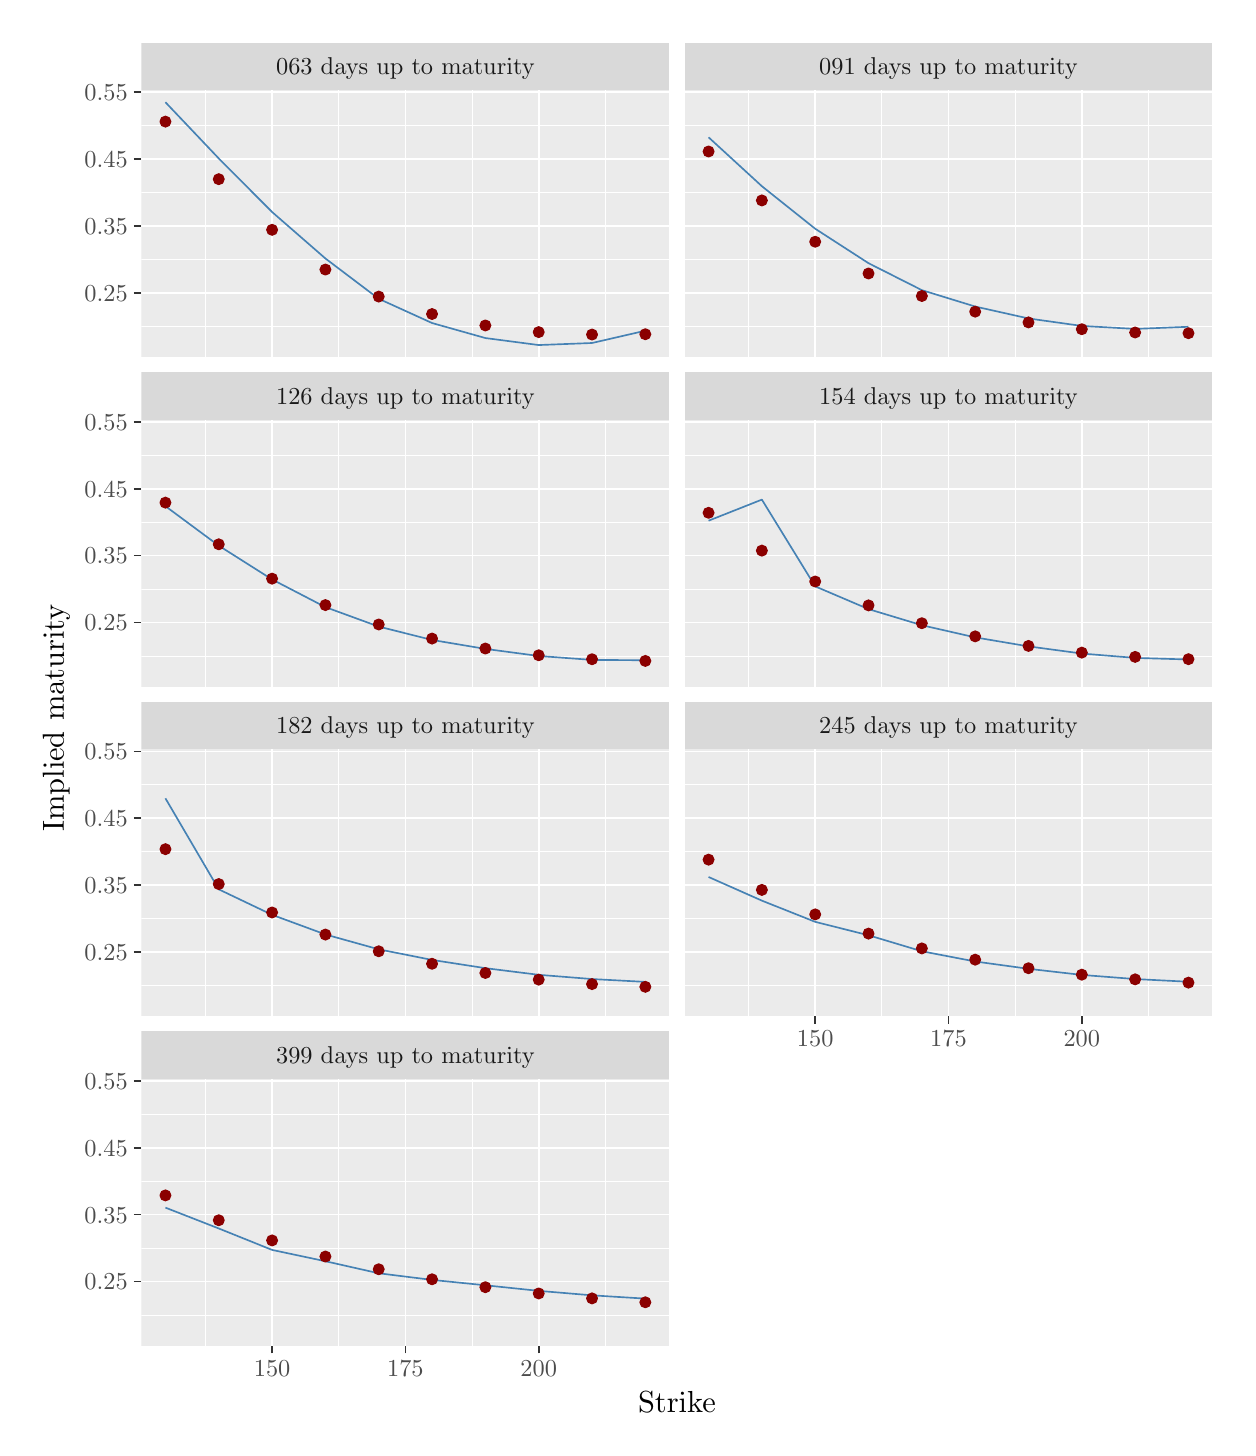
\begin{tikzpicture}[x=1pt,y=1pt]
\definecolor{fillColor}{RGB}{255,255,255}
\path[use as bounding box,fill=fillColor,fill opacity=0.00] (0,0) rectangle (433.62,505.89);
\begin{scope}
\path[clip] (  0.00,  0.00) rectangle (433.62,505.89);
\definecolor{drawColor}{RGB}{255,255,255}
\definecolor{fillColor}{RGB}{255,255,255}

\path[draw=drawColor,line width= 0.6pt,line join=round,line cap=round,fill=fillColor] (  0.00,  0.00) rectangle (433.62,505.89);
\end{scope}
\begin{scope}
\path[clip] ( 41.11,386.81) rectangle (231.87,483.33);
\definecolor{fillColor}{gray}{0.92}

\path[fill=fillColor] ( 41.11,386.81) rectangle (231.87,483.33);
\definecolor{drawColor}{RGB}{255,255,255}

\path[draw=drawColor,line width= 0.3pt,line join=round] ( 41.11,397.93) --
	(231.87,397.93);

\path[draw=drawColor,line width= 0.3pt,line join=round] ( 41.11,422.11) --
	(231.87,422.11);

\path[draw=drawColor,line width= 0.3pt,line join=round] ( 41.11,446.28) --
	(231.87,446.28);

\path[draw=drawColor,line width= 0.3pt,line join=round] ( 41.11,470.45) --
	(231.87,470.45);

\path[draw=drawColor,line width= 0.3pt,line join=round] ( 64.23,386.81) --
	( 64.23,483.33);

\path[draw=drawColor,line width= 0.3pt,line join=round] (112.40,386.81) --
	(112.40,483.33);

\path[draw=drawColor,line width= 0.3pt,line join=round] (160.57,386.81) --
	(160.57,483.33);

\path[draw=drawColor,line width= 0.3pt,line join=round] (208.74,386.81) --
	(208.74,483.33);

\path[draw=drawColor,line width= 0.6pt,line join=round] ( 41.11,410.02) --
	(231.87,410.02);

\path[draw=drawColor,line width= 0.6pt,line join=round] ( 41.11,434.19) --
	(231.87,434.19);

\path[draw=drawColor,line width= 0.6pt,line join=round] ( 41.11,458.37) --
	(231.87,458.37);

\path[draw=drawColor,line width= 0.6pt,line join=round] ( 41.11,482.54) --
	(231.87,482.54);

\path[draw=drawColor,line width= 0.6pt,line join=round] ( 88.32,386.81) --
	( 88.32,483.33);

\path[draw=drawColor,line width= 0.6pt,line join=round] (136.49,386.81) --
	(136.49,483.33);

\path[draw=drawColor,line width= 0.6pt,line join=round] (184.66,386.81) --
	(184.66,483.33);
\definecolor{drawColor}{RGB}{70,130,180}

\path[draw=drawColor,line width= 0.6pt,line join=round] ( 49.78,478.94) --
	( 69.05,458.63) --
	( 88.32,439.27) --
	(107.59,422.48) --
	(126.85,407.92) --
	(146.12,399.16) --
	(165.39,393.73) --
	(184.66,391.20) --
	(203.93,391.94) --
	(223.19,396.38);
\definecolor{drawColor}{RGB}{139,0,0}
\definecolor{fillColor}{RGB}{139,0,0}

\path[draw=drawColor,line width= 0.4pt,line join=round,line cap=round,fill=fillColor] ( 49.78,471.94) circle (  1.96);

\path[draw=drawColor,line width= 0.4pt,line join=round,line cap=round,fill=fillColor] ( 69.05,451.14) circle (  1.96);

\path[draw=drawColor,line width= 0.4pt,line join=round,line cap=round,fill=fillColor] ( 88.32,432.84) circle (  1.96);

\path[draw=drawColor,line width= 0.4pt,line join=round,line cap=round,fill=fillColor] (107.59,418.48) circle (  1.96);

\path[draw=drawColor,line width= 0.4pt,line join=round,line cap=round,fill=fillColor] (126.85,408.72) circle (  1.96);

\path[draw=drawColor,line width= 0.4pt,line join=round,line cap=round,fill=fillColor] (146.12,402.41) circle (  1.96);

\path[draw=drawColor,line width= 0.4pt,line join=round,line cap=round,fill=fillColor] (165.39,398.28) circle (  1.96);

\path[draw=drawColor,line width= 0.4pt,line join=round,line cap=round,fill=fillColor] (184.66,395.88) circle (  1.96);

\path[draw=drawColor,line width= 0.4pt,line join=round,line cap=round,fill=fillColor] (203.93,394.99) circle (  1.96);

\path[draw=drawColor,line width= 0.4pt,line join=round,line cap=round,fill=fillColor] (223.19,395.11) circle (  1.96);
\end{scope}
\begin{scope}
\path[clip] ( 41.11,267.74) rectangle (231.87,364.25);
\definecolor{fillColor}{gray}{0.92}

\path[fill=fillColor] ( 41.11,267.74) rectangle (231.87,364.25);
\definecolor{drawColor}{RGB}{255,255,255}

\path[draw=drawColor,line width= 0.3pt,line join=round] ( 41.11,278.86) --
	(231.87,278.86);

\path[draw=drawColor,line width= 0.3pt,line join=round] ( 41.11,303.03) --
	(231.87,303.03);

\path[draw=drawColor,line width= 0.3pt,line join=round] ( 41.11,327.20) --
	(231.87,327.20);

\path[draw=drawColor,line width= 0.3pt,line join=round] ( 41.11,351.38) --
	(231.87,351.38);

\path[draw=drawColor,line width= 0.3pt,line join=round] ( 64.23,267.74) --
	( 64.23,364.25);

\path[draw=drawColor,line width= 0.3pt,line join=round] (112.40,267.74) --
	(112.40,364.25);

\path[draw=drawColor,line width= 0.3pt,line join=round] (160.57,267.74) --
	(160.57,364.25);

\path[draw=drawColor,line width= 0.3pt,line join=round] (208.74,267.74) --
	(208.74,364.25);

\path[draw=drawColor,line width= 0.6pt,line join=round] ( 41.11,290.95) --
	(231.87,290.95);

\path[draw=drawColor,line width= 0.6pt,line join=round] ( 41.11,315.12) --
	(231.87,315.12);

\path[draw=drawColor,line width= 0.6pt,line join=round] ( 41.11,339.29) --
	(231.87,339.29);

\path[draw=drawColor,line width= 0.6pt,line join=round] ( 41.11,363.46) --
	(231.87,363.46);

\path[draw=drawColor,line width= 0.6pt,line join=round] ( 88.32,267.74) --
	( 88.32,364.25);

\path[draw=drawColor,line width= 0.6pt,line join=round] (136.49,267.74) --
	(136.49,364.25);

\path[draw=drawColor,line width= 0.6pt,line join=round] (184.66,267.74) --
	(184.66,364.25);
\definecolor{drawColor}{RGB}{70,130,180}

\path[draw=drawColor,line width= 0.6pt,line join=round] ( 49.78,332.98) --
	( 69.05,318.71) --
	( 88.32,306.50) --
	(107.59,296.51) --
	(126.85,289.47) --
	(146.12,284.64) --
	(165.39,281.41) --
	(184.66,278.85) --
	(203.93,277.43) --
	(223.19,277.30);
\definecolor{drawColor}{RGB}{139,0,0}
\definecolor{fillColor}{RGB}{139,0,0}

\path[draw=drawColor,line width= 0.4pt,line join=round,line cap=round,fill=fillColor] ( 49.78,334.26) circle (  1.96);

\path[draw=drawColor,line width= 0.4pt,line join=round,line cap=round,fill=fillColor] ( 69.05,319.20) circle (  1.96);

\path[draw=drawColor,line width= 0.4pt,line join=round,line cap=round,fill=fillColor] ( 88.32,306.79) circle (  1.96);

\path[draw=drawColor,line width= 0.4pt,line join=round,line cap=round,fill=fillColor] (107.59,297.24) circle (  1.96);

\path[draw=drawColor,line width= 0.4pt,line join=round,line cap=round,fill=fillColor] (126.85,290.23) circle (  1.96);

\path[draw=drawColor,line width= 0.4pt,line join=round,line cap=round,fill=fillColor] (146.12,285.14) circle (  1.96);

\path[draw=drawColor,line width= 0.4pt,line join=round,line cap=round,fill=fillColor] (165.39,281.54) circle (  1.96);

\path[draw=drawColor,line width= 0.4pt,line join=round,line cap=round,fill=fillColor] (184.66,279.10) circle (  1.96);

\path[draw=drawColor,line width= 0.4pt,line join=round,line cap=round,fill=fillColor] (203.93,277.67) circle (  1.96);

\path[draw=drawColor,line width= 0.4pt,line join=round,line cap=round,fill=fillColor] (223.19,277.06) circle (  1.96);
\end{scope}
\begin{scope}
\path[clip] ( 41.11,148.66) rectangle (231.87,245.18);
\definecolor{fillColor}{gray}{0.92}

\path[fill=fillColor] ( 41.11,148.66) rectangle (231.87,245.18);
\definecolor{drawColor}{RGB}{255,255,255}

\path[draw=drawColor,line width= 0.3pt,line join=round] ( 41.11,159.78) --
	(231.87,159.78);

\path[draw=drawColor,line width= 0.3pt,line join=round] ( 41.11,183.96) --
	(231.87,183.96);

\path[draw=drawColor,line width= 0.3pt,line join=round] ( 41.11,208.13) --
	(231.87,208.13);

\path[draw=drawColor,line width= 0.3pt,line join=round] ( 41.11,232.30) --
	(231.87,232.30);

\path[draw=drawColor,line width= 0.3pt,line join=round] ( 64.23,148.66) --
	( 64.23,245.18);

\path[draw=drawColor,line width= 0.3pt,line join=round] (112.40,148.66) --
	(112.40,245.18);

\path[draw=drawColor,line width= 0.3pt,line join=round] (160.57,148.66) --
	(160.57,245.18);

\path[draw=drawColor,line width= 0.3pt,line join=round] (208.74,148.66) --
	(208.74,245.18);

\path[draw=drawColor,line width= 0.6pt,line join=round] ( 41.11,171.87) --
	(231.87,171.87);

\path[draw=drawColor,line width= 0.6pt,line join=round] ( 41.11,196.04) --
	(231.87,196.04);

\path[draw=drawColor,line width= 0.6pt,line join=round] ( 41.11,220.21) --
	(231.87,220.21);

\path[draw=drawColor,line width= 0.6pt,line join=round] ( 41.11,244.39) --
	(231.87,244.39);

\path[draw=drawColor,line width= 0.6pt,line join=round] ( 88.32,148.66) --
	( 88.32,245.18);

\path[draw=drawColor,line width= 0.6pt,line join=round] (136.49,148.66) --
	(136.49,245.18);

\path[draw=drawColor,line width= 0.6pt,line join=round] (184.66,148.66) --
	(184.66,245.18);
\definecolor{drawColor}{RGB}{70,130,180}

\path[draw=drawColor,line width= 0.6pt,line join=round] ( 49.78,227.41) --
	( 69.05,194.52) --
	( 88.32,185.32) --
	(107.59,178.22) --
	(126.85,172.85) --
	(146.12,169.02) --
	(165.39,166.04) --
	(184.66,163.64) --
	(203.93,162.11) --
	(223.19,161.08);
\definecolor{drawColor}{RGB}{139,0,0}
\definecolor{fillColor}{RGB}{139,0,0}

\path[draw=drawColor,line width= 0.4pt,line join=round,line cap=round,fill=fillColor] ( 49.78,209.04) circle (  1.96);

\path[draw=drawColor,line width= 0.4pt,line join=round,line cap=round,fill=fillColor] ( 69.05,196.43) circle (  1.96);

\path[draw=drawColor,line width= 0.4pt,line join=round,line cap=round,fill=fillColor] ( 88.32,186.16) circle (  1.96);

\path[draw=drawColor,line width= 0.4pt,line join=round,line cap=round,fill=fillColor] (107.59,178.18) circle (  1.96);

\path[draw=drawColor,line width= 0.4pt,line join=round,line cap=round,fill=fillColor] (126.85,172.14) circle (  1.96);

\path[draw=drawColor,line width= 0.4pt,line join=round,line cap=round,fill=fillColor] (146.12,167.63) circle (  1.96);

\path[draw=drawColor,line width= 0.4pt,line join=round,line cap=round,fill=fillColor] (165.39,164.30) circle (  1.96);

\path[draw=drawColor,line width= 0.4pt,line join=round,line cap=round,fill=fillColor] (184.66,161.90) circle (  1.96);

\path[draw=drawColor,line width= 0.4pt,line join=round,line cap=round,fill=fillColor] (203.93,160.28) circle (  1.96);

\path[draw=drawColor,line width= 0.4pt,line join=round,line cap=round,fill=fillColor] (223.19,159.30) circle (  1.96);
\end{scope}
\begin{scope}
\path[clip] ( 41.11, 29.59) rectangle (231.87,126.10);
\definecolor{fillColor}{gray}{0.92}

\path[fill=fillColor] ( 41.11, 29.59) rectangle (231.87,126.10);
\definecolor{drawColor}{RGB}{255,255,255}

\path[draw=drawColor,line width= 0.3pt,line join=round] ( 41.11, 40.71) --
	(231.87, 40.71);

\path[draw=drawColor,line width= 0.3pt,line join=round] ( 41.11, 64.88) --
	(231.87, 64.88);

\path[draw=drawColor,line width= 0.3pt,line join=round] ( 41.11, 89.05) --
	(231.87, 89.05);

\path[draw=drawColor,line width= 0.3pt,line join=round] ( 41.11,113.22) --
	(231.87,113.22);

\path[draw=drawColor,line width= 0.3pt,line join=round] ( 64.23, 29.59) --
	( 64.23,126.10);

\path[draw=drawColor,line width= 0.3pt,line join=round] (112.40, 29.59) --
	(112.40,126.10);

\path[draw=drawColor,line width= 0.3pt,line join=round] (160.57, 29.59) --
	(160.57,126.10);

\path[draw=drawColor,line width= 0.3pt,line join=round] (208.74, 29.59) --
	(208.74,126.10);

\path[draw=drawColor,line width= 0.6pt,line join=round] ( 41.11, 52.79) --
	(231.87, 52.79);

\path[draw=drawColor,line width= 0.6pt,line join=round] ( 41.11, 76.97) --
	(231.87, 76.97);

\path[draw=drawColor,line width= 0.6pt,line join=round] ( 41.11,101.14) --
	(231.87,101.14);

\path[draw=drawColor,line width= 0.6pt,line join=round] ( 41.11,125.31) --
	(231.87,125.31);

\path[draw=drawColor,line width= 0.6pt,line join=round] ( 88.32, 29.59) --
	( 88.32,126.10);

\path[draw=drawColor,line width= 0.6pt,line join=round] (136.49, 29.59) --
	(136.49,126.10);

\path[draw=drawColor,line width= 0.6pt,line join=round] (184.66, 29.59) --
	(184.66,126.10);
\definecolor{drawColor}{RGB}{70,130,180}

\path[draw=drawColor,line width= 0.6pt,line join=round] ( 49.78, 79.51) --
	( 69.05, 71.98) --
	( 88.32, 64.23) --
	(107.59, 60.14) --
	(126.85, 55.79) --
	(146.12, 53.40) --
	(165.39, 51.45) --
	(184.66, 49.44) --
	(203.93, 47.82) --
	(223.19, 46.63);
\definecolor{drawColor}{RGB}{139,0,0}
\definecolor{fillColor}{RGB}{139,0,0}

\path[draw=drawColor,line width= 0.4pt,line join=round,line cap=round,fill=fillColor] ( 49.78, 83.93) circle (  1.96);

\path[draw=drawColor,line width= 0.4pt,line join=round,line cap=round,fill=fillColor] ( 69.05, 74.95) circle (  1.96);

\path[draw=drawColor,line width= 0.4pt,line join=round,line cap=round,fill=fillColor] ( 88.32, 67.66) circle (  1.96);

\path[draw=drawColor,line width= 0.4pt,line join=round,line cap=round,fill=fillColor] (107.59, 61.84) circle (  1.96);

\path[draw=drawColor,line width= 0.4pt,line join=round,line cap=round,fill=fillColor] (126.85, 57.24) circle (  1.96);

\path[draw=drawColor,line width= 0.4pt,line join=round,line cap=round,fill=fillColor] (146.12, 53.62) circle (  1.96);

\path[draw=drawColor,line width= 0.4pt,line join=round,line cap=round,fill=fillColor] (165.39, 50.76) circle (  1.96);

\path[draw=drawColor,line width= 0.4pt,line join=round,line cap=round,fill=fillColor] (184.66, 48.50) circle (  1.96);

\path[draw=drawColor,line width= 0.4pt,line join=round,line cap=round,fill=fillColor] (203.93, 46.72) circle (  1.96);

\path[draw=drawColor,line width= 0.4pt,line join=round,line cap=round,fill=fillColor] (223.19, 45.31) circle (  1.96);
\end{scope}
\begin{scope}
\path[clip] (237.37,386.81) rectangle (428.12,483.33);
\definecolor{fillColor}{gray}{0.92}

\path[fill=fillColor] (237.37,386.81) rectangle (428.12,483.33);
\definecolor{drawColor}{RGB}{255,255,255}

\path[draw=drawColor,line width= 0.3pt,line join=round] (237.37,397.93) --
	(428.12,397.93);

\path[draw=drawColor,line width= 0.3pt,line join=round] (237.37,422.11) --
	(428.12,422.11);

\path[draw=drawColor,line width= 0.3pt,line join=round] (237.37,446.28) --
	(428.12,446.28);

\path[draw=drawColor,line width= 0.3pt,line join=round] (237.37,470.45) --
	(428.12,470.45);

\path[draw=drawColor,line width= 0.3pt,line join=round] (260.49,386.81) --
	(260.49,483.33);

\path[draw=drawColor,line width= 0.3pt,line join=round] (308.66,386.81) --
	(308.66,483.33);

\path[draw=drawColor,line width= 0.3pt,line join=round] (356.83,386.81) --
	(356.83,483.33);

\path[draw=drawColor,line width= 0.3pt,line join=round] (405.00,386.81) --
	(405.00,483.33);

\path[draw=drawColor,line width= 0.6pt,line join=round] (237.37,410.02) --
	(428.12,410.02);

\path[draw=drawColor,line width= 0.6pt,line join=round] (237.37,434.19) --
	(428.12,434.19);

\path[draw=drawColor,line width= 0.6pt,line join=round] (237.37,458.37) --
	(428.12,458.37);

\path[draw=drawColor,line width= 0.6pt,line join=round] (237.37,482.54) --
	(428.12,482.54);

\path[draw=drawColor,line width= 0.6pt,line join=round] (284.57,386.81) --
	(284.57,483.33);

\path[draw=drawColor,line width= 0.6pt,line join=round] (332.74,386.81) --
	(332.74,483.33);

\path[draw=drawColor,line width= 0.6pt,line join=round] (380.91,386.81) --
	(380.91,483.33);
\definecolor{drawColor}{RGB}{70,130,180}

\path[draw=drawColor,line width= 0.6pt,line join=round] (246.04,466.27) --
	(265.30,448.60) --
	(284.57,433.23) --
	(303.84,420.78) --
	(323.11,411.04) --
	(342.38,405.12) --
	(361.64,400.81) --
	(380.91,398.11) --
	(400.18,397.03) --
	(419.45,397.80);
\definecolor{drawColor}{RGB}{139,0,0}
\definecolor{fillColor}{RGB}{139,0,0}

\path[draw=drawColor,line width= 0.4pt,line join=round,line cap=round,fill=fillColor] (246.04,461.14) circle (  1.96);

\path[draw=drawColor,line width= 0.4pt,line join=round,line cap=round,fill=fillColor] (265.30,443.46) circle (  1.96);

\path[draw=drawColor,line width= 0.4pt,line join=round,line cap=round,fill=fillColor] (284.57,428.53) circle (  1.96);

\path[draw=drawColor,line width= 0.4pt,line join=round,line cap=round,fill=fillColor] (303.84,417.06) circle (  1.96);

\path[draw=drawColor,line width= 0.4pt,line join=round,line cap=round,fill=fillColor] (323.11,408.92) circle (  1.96);

\path[draw=drawColor,line width= 0.4pt,line join=round,line cap=round,fill=fillColor] (342.38,403.27) circle (  1.96);

\path[draw=drawColor,line width= 0.4pt,line join=round,line cap=round,fill=fillColor] (361.64,399.38) circle (  1.96);

\path[draw=drawColor,line width= 0.4pt,line join=round,line cap=round,fill=fillColor] (380.91,396.93) circle (  1.96);

\path[draw=drawColor,line width= 0.4pt,line join=round,line cap=round,fill=fillColor] (400.18,395.74) circle (  1.96);

\path[draw=drawColor,line width= 0.4pt,line join=round,line cap=round,fill=fillColor] (419.45,395.48) circle (  1.96);
\end{scope}
\begin{scope}
\path[clip] (237.37,267.74) rectangle (428.12,364.25);
\definecolor{fillColor}{gray}{0.92}

\path[fill=fillColor] (237.37,267.74) rectangle (428.12,364.25);
\definecolor{drawColor}{RGB}{255,255,255}

\path[draw=drawColor,line width= 0.3pt,line join=round] (237.37,278.86) --
	(428.12,278.86);

\path[draw=drawColor,line width= 0.3pt,line join=round] (237.37,303.03) --
	(428.12,303.03);

\path[draw=drawColor,line width= 0.3pt,line join=round] (237.37,327.20) --
	(428.12,327.20);

\path[draw=drawColor,line width= 0.3pt,line join=round] (237.37,351.38) --
	(428.12,351.38);

\path[draw=drawColor,line width= 0.3pt,line join=round] (260.49,267.74) --
	(260.49,364.25);

\path[draw=drawColor,line width= 0.3pt,line join=round] (308.66,267.74) --
	(308.66,364.25);

\path[draw=drawColor,line width= 0.3pt,line join=round] (356.83,267.74) --
	(356.83,364.25);

\path[draw=drawColor,line width= 0.3pt,line join=round] (405.00,267.74) --
	(405.00,364.25);

\path[draw=drawColor,line width= 0.6pt,line join=round] (237.37,290.95) --
	(428.12,290.95);

\path[draw=drawColor,line width= 0.6pt,line join=round] (237.37,315.12) --
	(428.12,315.12);

\path[draw=drawColor,line width= 0.6pt,line join=round] (237.37,339.29) --
	(428.12,339.29);

\path[draw=drawColor,line width= 0.6pt,line join=round] (237.37,363.46) --
	(428.12,363.46);

\path[draw=drawColor,line width= 0.6pt,line join=round] (284.57,267.74) --
	(284.57,364.25);

\path[draw=drawColor,line width= 0.6pt,line join=round] (332.74,267.74) --
	(332.74,364.25);

\path[draw=drawColor,line width= 0.6pt,line join=round] (380.91,267.74) --
	(380.91,364.25);
\definecolor{drawColor}{RGB}{70,130,180}

\path[draw=drawColor,line width= 0.6pt,line join=round] (246.04,327.73) --
	(265.30,335.35) --
	(284.57,304.00) --
	(303.84,295.78) --
	(323.11,289.96) --
	(342.38,285.57) --
	(361.64,282.32) --
	(380.91,279.73) --
	(400.18,278.15) --
	(419.45,277.58);
\definecolor{drawColor}{RGB}{139,0,0}
\definecolor{fillColor}{RGB}{139,0,0}

\path[draw=drawColor,line width= 0.4pt,line join=round,line cap=round,fill=fillColor] (246.04,330.58) circle (  1.96);

\path[draw=drawColor,line width= 0.4pt,line join=round,line cap=round,fill=fillColor] (265.30,316.92) circle (  1.96);

\path[draw=drawColor,line width= 0.4pt,line join=round,line cap=round,fill=fillColor] (284.57,305.76) circle (  1.96);

\path[draw=drawColor,line width= 0.4pt,line join=round,line cap=round,fill=fillColor] (303.84,297.13) circle (  1.96);

\path[draw=drawColor,line width= 0.4pt,line join=round,line cap=round,fill=fillColor] (323.11,290.69) circle (  1.96);

\path[draw=drawColor,line width= 0.4pt,line join=round,line cap=round,fill=fillColor] (342.38,285.94) circle (  1.96);

\path[draw=drawColor,line width= 0.4pt,line join=round,line cap=round,fill=fillColor] (361.64,282.48) circle (  1.96);

\path[draw=drawColor,line width= 0.4pt,line join=round,line cap=round,fill=fillColor] (380.91,280.06) circle (  1.96);

\path[draw=drawColor,line width= 0.4pt,line join=round,line cap=round,fill=fillColor] (400.18,278.52) circle (  1.96);

\path[draw=drawColor,line width= 0.4pt,line join=round,line cap=round,fill=fillColor] (419.45,277.69) circle (  1.96);
\end{scope}
\begin{scope}
\path[clip] (237.37,148.66) rectangle (428.12,245.18);
\definecolor{fillColor}{gray}{0.92}

\path[fill=fillColor] (237.37,148.66) rectangle (428.12,245.18);
\definecolor{drawColor}{RGB}{255,255,255}

\path[draw=drawColor,line width= 0.3pt,line join=round] (237.37,159.78) --
	(428.12,159.78);

\path[draw=drawColor,line width= 0.3pt,line join=round] (237.37,183.96) --
	(428.12,183.96);

\path[draw=drawColor,line width= 0.3pt,line join=round] (237.37,208.13) --
	(428.12,208.13);

\path[draw=drawColor,line width= 0.3pt,line join=round] (237.37,232.30) --
	(428.12,232.30);

\path[draw=drawColor,line width= 0.3pt,line join=round] (260.49,148.66) --
	(260.49,245.18);

\path[draw=drawColor,line width= 0.3pt,line join=round] (308.66,148.66) --
	(308.66,245.18);

\path[draw=drawColor,line width= 0.3pt,line join=round] (356.83,148.66) --
	(356.83,245.18);

\path[draw=drawColor,line width= 0.3pt,line join=round] (405.00,148.66) --
	(405.00,245.18);

\path[draw=drawColor,line width= 0.6pt,line join=round] (237.37,171.87) --
	(428.12,171.87);

\path[draw=drawColor,line width= 0.6pt,line join=round] (237.37,196.04) --
	(428.12,196.04);

\path[draw=drawColor,line width= 0.6pt,line join=round] (237.37,220.21) --
	(428.12,220.21);

\path[draw=drawColor,line width= 0.6pt,line join=round] (237.37,244.39) --
	(428.12,244.39);

\path[draw=drawColor,line width= 0.6pt,line join=round] (284.57,148.66) --
	(284.57,245.18);

\path[draw=drawColor,line width= 0.6pt,line join=round] (332.74,148.66) --
	(332.74,245.18);

\path[draw=drawColor,line width= 0.6pt,line join=round] (380.91,148.66) --
	(380.91,245.18);
\definecolor{drawColor}{RGB}{70,130,180}

\path[draw=drawColor,line width= 0.6pt,line join=round] (246.04,198.99) --
	(265.30,190.44) --
	(284.57,182.78) --
	(303.84,177.93) --
	(323.11,172.15) --
	(342.38,168.45) --
	(361.64,165.81) --
	(380.91,163.60) --
	(400.18,162.11) --
	(419.45,161.13);
\definecolor{drawColor}{RGB}{139,0,0}
\definecolor{fillColor}{RGB}{139,0,0}

\path[draw=drawColor,line width= 0.4pt,line join=round,line cap=round,fill=fillColor] (246.04,205.25) circle (  1.96);

\path[draw=drawColor,line width= 0.4pt,line join=round,line cap=round,fill=fillColor] (265.30,194.32) circle (  1.96);

\path[draw=drawColor,line width= 0.4pt,line join=round,line cap=round,fill=fillColor] (284.57,185.47) circle (  1.96);

\path[draw=drawColor,line width= 0.4pt,line join=round,line cap=round,fill=fillColor] (303.84,178.53) circle (  1.96);

\path[draw=drawColor,line width= 0.4pt,line join=round,line cap=round,fill=fillColor] (323.11,173.18) circle (  1.96);

\path[draw=drawColor,line width= 0.4pt,line join=round,line cap=round,fill=fillColor] (342.38,169.11) circle (  1.96);

\path[draw=drawColor,line width= 0.4pt,line join=round,line cap=round,fill=fillColor] (361.64,166.02) circle (  1.96);

\path[draw=drawColor,line width= 0.4pt,line join=round,line cap=round,fill=fillColor] (380.91,163.69) circle (  1.96);

\path[draw=drawColor,line width= 0.4pt,line join=round,line cap=round,fill=fillColor] (400.18,162.00) circle (  1.96);

\path[draw=drawColor,line width= 0.4pt,line join=round,line cap=round,fill=fillColor] (419.45,160.81) circle (  1.96);
\end{scope}
\begin{scope}
\path[clip] ( 41.11,126.10) rectangle (231.87,143.16);
\definecolor{fillColor}{gray}{0.85}

\path[fill=fillColor] ( 41.11,126.10) rectangle (231.87,143.16);
\definecolor{drawColor}{gray}{0.10}

\node[text=drawColor,anchor=base,inner sep=0pt, outer sep=0pt, scale=  0.88] at (136.49,131.60) {399 days up to maturity};
\end{scope}
\begin{scope}
\path[clip] ( 41.11,245.18) rectangle (231.87,262.24);
\definecolor{fillColor}{gray}{0.85}

\path[fill=fillColor] ( 41.11,245.18) rectangle (231.87,262.24);
\definecolor{drawColor}{gray}{0.10}

\node[text=drawColor,anchor=base,inner sep=0pt, outer sep=0pt, scale=  0.88] at (136.49,250.68) {182 days up to maturity};
\end{scope}
\begin{scope}
\path[clip] (237.37,245.18) rectangle (428.12,262.24);
\definecolor{fillColor}{gray}{0.85}

\path[fill=fillColor] (237.37,245.18) rectangle (428.12,262.24);
\definecolor{drawColor}{gray}{0.10}

\node[text=drawColor,anchor=base,inner sep=0pt, outer sep=0pt, scale=  0.88] at (332.74,250.68) {245 days up to maturity};
\end{scope}
\begin{scope}
\path[clip] ( 41.11,364.25) rectangle (231.87,381.31);
\definecolor{fillColor}{gray}{0.85}

\path[fill=fillColor] ( 41.11,364.25) rectangle (231.87,381.31);
\definecolor{drawColor}{gray}{0.10}

\node[text=drawColor,anchor=base,inner sep=0pt, outer sep=0pt, scale=  0.88] at (136.49,369.75) {126 days up to maturity};
\end{scope}
\begin{scope}
\path[clip] (237.37,364.25) rectangle (428.12,381.31);
\definecolor{fillColor}{gray}{0.85}

\path[fill=fillColor] (237.37,364.25) rectangle (428.12,381.31);
\definecolor{drawColor}{gray}{0.10}

\node[text=drawColor,anchor=base,inner sep=0pt, outer sep=0pt, scale=  0.88] at (332.74,369.75) {154 days up to maturity};
\end{scope}
\begin{scope}
\path[clip] ( 41.11,483.33) rectangle (231.87,500.39);
\definecolor{fillColor}{gray}{0.85}

\path[fill=fillColor] ( 41.11,483.33) rectangle (231.87,500.39);
\definecolor{drawColor}{gray}{0.10}

\node[text=drawColor,anchor=base,inner sep=0pt, outer sep=0pt, scale=  0.88] at (136.49,488.83) {063 days up to maturity};
\end{scope}
\begin{scope}
\path[clip] (237.37,483.33) rectangle (428.12,500.39);
\definecolor{fillColor}{gray}{0.85}

\path[fill=fillColor] (237.37,483.33) rectangle (428.12,500.39);
\definecolor{drawColor}{gray}{0.10}

\node[text=drawColor,anchor=base,inner sep=0pt, outer sep=0pt, scale=  0.88] at (332.74,488.83) {091 days up to maturity};
\end{scope}
\begin{scope}
\path[clip] (  0.00,  0.00) rectangle (433.62,505.89);
\definecolor{drawColor}{gray}{0.20}

\path[draw=drawColor,line width= 0.6pt,line join=round] ( 88.32, 26.84) --
	( 88.32, 29.59);

\path[draw=drawColor,line width= 0.6pt,line join=round] (136.49, 26.84) --
	(136.49, 29.59);

\path[draw=drawColor,line width= 0.6pt,line join=round] (184.66, 26.84) --
	(184.66, 29.59);
\end{scope}
\begin{scope}
\path[clip] (  0.00,  0.00) rectangle (433.62,505.89);
\definecolor{drawColor}{gray}{0.30}

\node[text=drawColor,anchor=base,inner sep=0pt, outer sep=0pt, scale=  0.88] at ( 88.32, 18.58) {150};

\node[text=drawColor,anchor=base,inner sep=0pt, outer sep=0pt, scale=  0.88] at (136.49, 18.58) {175};

\node[text=drawColor,anchor=base,inner sep=0pt, outer sep=0pt, scale=  0.88] at (184.66, 18.58) {200};
\end{scope}
\begin{scope}
\path[clip] (  0.00,  0.00) rectangle (433.62,505.89);
\definecolor{drawColor}{gray}{0.20}

\path[draw=drawColor,line width= 0.6pt,line join=round] (284.57,145.91) --
	(284.57,148.66);

\path[draw=drawColor,line width= 0.6pt,line join=round] (332.74,145.91) --
	(332.74,148.66);

\path[draw=drawColor,line width= 0.6pt,line join=round] (380.91,145.91) --
	(380.91,148.66);
\end{scope}
\begin{scope}
\path[clip] (  0.00,  0.00) rectangle (433.62,505.89);
\definecolor{drawColor}{gray}{0.30}

\node[text=drawColor,anchor=base,inner sep=0pt, outer sep=0pt, scale=  0.88] at (284.57,137.65) {150};

\node[text=drawColor,anchor=base,inner sep=0pt, outer sep=0pt, scale=  0.88] at (332.74,137.65) {175};

\node[text=drawColor,anchor=base,inner sep=0pt, outer sep=0pt, scale=  0.88] at (380.91,137.65) {200};
\end{scope}
\begin{scope}
\path[clip] (  0.00,  0.00) rectangle (433.62,505.89);
\definecolor{drawColor}{gray}{0.30}

\node[text=drawColor,anchor=base east,inner sep=0pt, outer sep=0pt, scale=  0.88] at ( 36.16,406.99) {0.25};

\node[text=drawColor,anchor=base east,inner sep=0pt, outer sep=0pt, scale=  0.88] at ( 36.16,431.16) {0.35};

\node[text=drawColor,anchor=base east,inner sep=0pt, outer sep=0pt, scale=  0.88] at ( 36.16,455.34) {0.45};

\node[text=drawColor,anchor=base east,inner sep=0pt, outer sep=0pt, scale=  0.88] at ( 36.16,479.51) {0.55};
\end{scope}
\begin{scope}
\path[clip] (  0.00,  0.00) rectangle (433.62,505.89);
\definecolor{drawColor}{gray}{0.20}

\path[draw=drawColor,line width= 0.6pt,line join=round] ( 38.36,410.02) --
	( 41.11,410.02);

\path[draw=drawColor,line width= 0.6pt,line join=round] ( 38.36,434.19) --
	( 41.11,434.19);

\path[draw=drawColor,line width= 0.6pt,line join=round] ( 38.36,458.37) --
	( 41.11,458.37);

\path[draw=drawColor,line width= 0.6pt,line join=round] ( 38.36,482.54) --
	( 41.11,482.54);
\end{scope}
\begin{scope}
\path[clip] (  0.00,  0.00) rectangle (433.62,505.89);
\definecolor{drawColor}{gray}{0.30}

\node[text=drawColor,anchor=base east,inner sep=0pt, outer sep=0pt, scale=  0.88] at ( 36.16,287.91) {0.25};

\node[text=drawColor,anchor=base east,inner sep=0pt, outer sep=0pt, scale=  0.88] at ( 36.16,312.09) {0.35};

\node[text=drawColor,anchor=base east,inner sep=0pt, outer sep=0pt, scale=  0.88] at ( 36.16,336.26) {0.45};

\node[text=drawColor,anchor=base east,inner sep=0pt, outer sep=0pt, scale=  0.88] at ( 36.16,360.43) {0.55};
\end{scope}
\begin{scope}
\path[clip] (  0.00,  0.00) rectangle (433.62,505.89);
\definecolor{drawColor}{gray}{0.20}

\path[draw=drawColor,line width= 0.6pt,line join=round] ( 38.36,290.95) --
	( 41.11,290.95);

\path[draw=drawColor,line width= 0.6pt,line join=round] ( 38.36,315.12) --
	( 41.11,315.12);

\path[draw=drawColor,line width= 0.6pt,line join=round] ( 38.36,339.29) --
	( 41.11,339.29);

\path[draw=drawColor,line width= 0.6pt,line join=round] ( 38.36,363.46) --
	( 41.11,363.46);
\end{scope}
\begin{scope}
\path[clip] (  0.00,  0.00) rectangle (433.62,505.89);
\definecolor{drawColor}{gray}{0.30}

\node[text=drawColor,anchor=base east,inner sep=0pt, outer sep=0pt, scale=  0.88] at ( 36.16,168.84) {0.25};

\node[text=drawColor,anchor=base east,inner sep=0pt, outer sep=0pt, scale=  0.88] at ( 36.16,193.01) {0.35};

\node[text=drawColor,anchor=base east,inner sep=0pt, outer sep=0pt, scale=  0.88] at ( 36.16,217.18) {0.45};

\node[text=drawColor,anchor=base east,inner sep=0pt, outer sep=0pt, scale=  0.88] at ( 36.16,241.36) {0.55};
\end{scope}
\begin{scope}
\path[clip] (  0.00,  0.00) rectangle (433.62,505.89);
\definecolor{drawColor}{gray}{0.20}

\path[draw=drawColor,line width= 0.6pt,line join=round] ( 38.36,171.87) --
	( 41.11,171.87);

\path[draw=drawColor,line width= 0.6pt,line join=round] ( 38.36,196.04) --
	( 41.11,196.04);

\path[draw=drawColor,line width= 0.6pt,line join=round] ( 38.36,220.21) --
	( 41.11,220.21);

\path[draw=drawColor,line width= 0.6pt,line join=round] ( 38.36,244.39) --
	( 41.11,244.39);
\end{scope}
\begin{scope}
\path[clip] (  0.00,  0.00) rectangle (433.62,505.89);
\definecolor{drawColor}{gray}{0.30}

\node[text=drawColor,anchor=base east,inner sep=0pt, outer sep=0pt, scale=  0.88] at ( 36.16, 49.76) {0.25};

\node[text=drawColor,anchor=base east,inner sep=0pt, outer sep=0pt, scale=  0.88] at ( 36.16, 73.94) {0.35};

\node[text=drawColor,anchor=base east,inner sep=0pt, outer sep=0pt, scale=  0.88] at ( 36.16, 98.11) {0.45};

\node[text=drawColor,anchor=base east,inner sep=0pt, outer sep=0pt, scale=  0.88] at ( 36.16,122.28) {0.55};
\end{scope}
\begin{scope}
\path[clip] (  0.00,  0.00) rectangle (433.62,505.89);
\definecolor{drawColor}{gray}{0.20}

\path[draw=drawColor,line width= 0.6pt,line join=round] ( 38.36, 52.79) --
	( 41.11, 52.79);

\path[draw=drawColor,line width= 0.6pt,line join=round] ( 38.36, 76.97) --
	( 41.11, 76.97);

\path[draw=drawColor,line width= 0.6pt,line join=round] ( 38.36,101.14) --
	( 41.11,101.14);

\path[draw=drawColor,line width= 0.6pt,line join=round] ( 38.36,125.31) --
	( 41.11,125.31);
\end{scope}
\begin{scope}
\path[clip] (  0.00,  0.00) rectangle (433.62,505.89);
\definecolor{drawColor}{RGB}{0,0,0}

\node[text=drawColor,anchor=base,inner sep=0pt, outer sep=0pt, scale=  1.10] at (234.62,  5.50) {Strike};
\end{scope}
\begin{scope}
\path[clip] (  0.00,  0.00) rectangle (433.62,505.89);
\definecolor{drawColor}{RGB}{0,0,0}

\node[text=drawColor,rotate= 90.00,anchor=base,inner sep=0pt, outer sep=0pt, scale=  1.10] at ( 13.08,256.46) {Implied maturity};
\end{scope}
\end{tikzpicture}

  \caption{Implied volatility of Apple option prices computed with HSV}
  \floatfoot{The blue curves represent the implied volatility computed from the option market data on Apple while the ................
  }
  \label{p:methodology:impliedvol:aapl:heston}
\end{figure}


Consequently, the set \ref{eq:methodology:arg:heston:riskneutral} is the one I will use together with the \textit{hsv\_call} function whenever I have to compute option price using the HSV model on Apple data for the purpose of that master thesis.

%%%%%%%%%%%%%%%%%%%%%%%%%%%%%%%%%%%%%%%%%%%%%%%%%%%%%%%%%%%%%%%%%%%%%%%%%%%%%%%%
\subsubsection*{Calibration of parameters for time series}

The set \ref{eq:methodology:arg:heston:riskneutral} is calibrated under the risk-neutral world and cannot, therefore, be used as is to simulate the dummy time-series that will be used in the analysis aimed to measure the delta hedging performance.
Furthermore, in addition to those parameters, the drift rate $\alpha$ has to be estimated as well. It was not present in the set  \ref{eq:methodology:arg:heston:riskneutral} because it is not taken into account in the computation of the options prices.

\Cref{p:methodology:density:aapl:heston:riskneutral} shows the empirical density curves illustrating the distributions of the log-returns computed either from historical Apple stock data for the blue curve or from dummy time series generated by the function \textit{hsv\_ts()} fed with the risk-neutral parameters\ref{eq:methodology:arg:heston:riskneutral}, for the red one.


\begin{figure}[ht]
  \centering
  % Created by tikzDevice version 0.11 on 2018-07-18 23:13:44
% !TEX encoding = UTF-8 Unicode
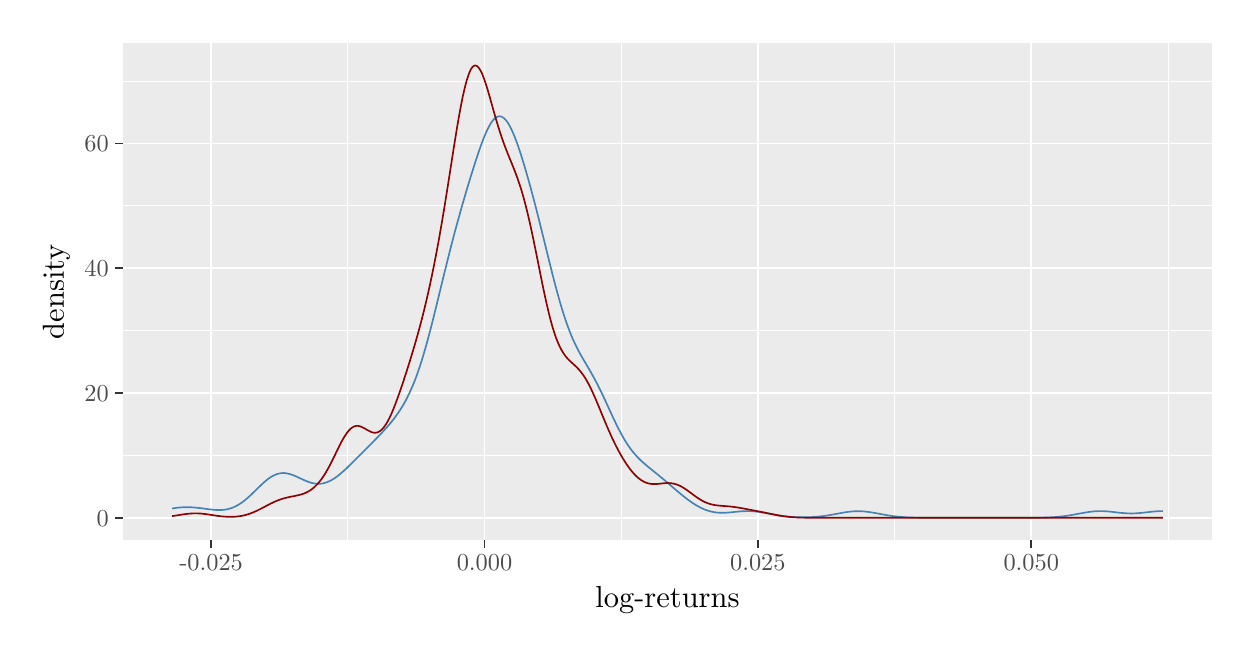
\begin{tikzpicture}[x=1pt,y=1pt]
\definecolor{fillColor}{RGB}{255,255,255}
\path[use as bounding box,fill=fillColor,fill opacity=0.00] (0,0) rectangle (433.62,216.81);
\begin{scope}
\path[clip] (  0.00,  0.00) rectangle (433.62,216.81);
\definecolor{drawColor}{RGB}{255,255,255}
\definecolor{fillColor}{RGB}{255,255,255}

\path[draw=drawColor,line width= 0.6pt,line join=round,line cap=round,fill=fillColor] (  0.00,  0.00) rectangle (433.62,216.81);
\end{scope}
\begin{scope}
\path[clip] ( 34.27, 31.53) rectangle (428.12,211.31);
\definecolor{fillColor}{gray}{0.92}

\path[fill=fillColor] ( 34.27, 31.53) rectangle (428.12,211.31);
\definecolor{drawColor}{RGB}{255,255,255}

\path[draw=drawColor,line width= 0.3pt,line join=round] ( 34.27, 62.24) --
	(428.12, 62.24);

\path[draw=drawColor,line width= 0.3pt,line join=round] ( 34.27,107.32) --
	(428.12,107.32);

\path[draw=drawColor,line width= 0.3pt,line join=round] ( 34.27,152.40) --
	(428.12,152.40);

\path[draw=drawColor,line width= 0.3pt,line join=round] ( 34.27,197.48) --
	(428.12,197.48);

\path[draw=drawColor,line width= 0.3pt,line join=round] (115.67, 31.53) --
	(115.67,211.31);

\path[draw=drawColor,line width= 0.3pt,line join=round] (214.46, 31.53) --
	(214.46,211.31);

\path[draw=drawColor,line width= 0.3pt,line join=round] (313.25, 31.53) --
	(313.25,211.31);

\path[draw=drawColor,line width= 0.3pt,line join=round] (412.03, 31.53) --
	(412.03,211.31);

\path[draw=drawColor,line width= 0.6pt,line join=round] ( 34.27, 39.70) --
	(428.12, 39.70);

\path[draw=drawColor,line width= 0.6pt,line join=round] ( 34.27, 84.78) --
	(428.12, 84.78);

\path[draw=drawColor,line width= 0.6pt,line join=round] ( 34.27,129.86) --
	(428.12,129.86);

\path[draw=drawColor,line width= 0.6pt,line join=round] ( 34.27,174.94) --
	(428.12,174.94);

\path[draw=drawColor,line width= 0.6pt,line join=round] ( 66.28, 31.53) --
	( 66.28,211.31);

\path[draw=drawColor,line width= 0.6pt,line join=round] (165.07, 31.53) --
	(165.07,211.31);

\path[draw=drawColor,line width= 0.6pt,line join=round] (263.85, 31.53) --
	(263.85,211.31);

\path[draw=drawColor,line width= 0.6pt,line join=round] (362.64, 31.53) --
	(362.64,211.31);
\definecolor{drawColor}{RGB}{70,130,180}

\path[draw=drawColor,line width= 0.6pt,line join=round] ( 52.17, 43.06) --
	( 52.87, 43.17) --
	( 53.57, 43.27) --
	( 54.27, 43.36) --
	( 54.97, 43.42) --
	( 55.67, 43.47) --
	( 56.37, 43.51) --
	( 57.07, 43.53) --
	( 57.78, 43.53) --
	( 58.48, 43.52) --
	( 59.18, 43.49) --
	( 59.88, 43.45) --
	( 60.58, 43.39) --
	( 61.28, 43.33) --
	( 61.98, 43.25) --
	( 62.68, 43.17) --
	( 63.38, 43.07) --
	( 64.08, 42.98) --
	( 64.78, 42.88) --
	( 65.48, 42.79) --
	( 66.18, 42.71) --
	( 66.88, 42.63) --
	( 67.59, 42.57) --
	( 68.29, 42.52) --
	( 68.99, 42.50) --
	( 69.69, 42.51) --
	( 70.39, 42.55) --
	( 71.09, 42.62) --
	( 71.79, 42.73) --
	( 72.49, 42.88) --
	( 73.19, 43.07) --
	( 73.89, 43.31) --
	( 74.59, 43.60) --
	( 75.29, 43.94) --
	( 75.99, 44.32) --
	( 76.69, 44.75) --
	( 77.39, 45.22) --
	( 78.10, 45.74) --
	( 78.80, 46.31) --
	( 79.50, 46.91) --
	( 80.20, 47.54) --
	( 80.90, 48.19) --
	( 81.60, 48.87) --
	( 82.30, 49.55) --
	( 83.00, 50.24) --
	( 83.70, 50.92) --
	( 84.40, 51.59) --
	( 85.10, 52.24) --
	( 85.80, 52.86) --
	( 86.50, 53.44) --
	( 87.20, 53.97) --
	( 87.90, 54.44) --
	( 88.61, 54.85) --
	( 89.31, 55.19) --
	( 90.01, 55.47) --
	( 90.71, 55.67) --
	( 91.41, 55.81) --
	( 92.11, 55.87) --
	( 92.81, 55.86) --
	( 93.51, 55.78) --
	( 94.21, 55.64) --
	( 94.91, 55.45) --
	( 95.61, 55.22) --
	( 96.31, 54.95) --
	( 97.01, 54.65) --
	( 97.71, 54.33) --
	( 98.42, 54.00) --
	( 99.12, 53.67) --
	( 99.82, 53.35) --
	(100.52, 53.05) --
	(101.22, 52.77) --
	(101.92, 52.52) --
	(102.62, 52.32) --
	(103.32, 52.16) --
	(104.02, 52.05) --
	(104.72, 51.99) --
	(105.42, 51.99) --
	(106.12, 52.05) --
	(106.82, 52.16) --
	(107.52, 52.35) --
	(108.22, 52.59) --
	(108.93, 52.89) --
	(109.63, 53.24) --
	(110.33, 53.64) --
	(111.03, 54.09) --
	(111.73, 54.59) --
	(112.43, 55.14) --
	(113.13, 55.71) --
	(113.83, 56.32) --
	(114.53, 56.95) --
	(115.23, 57.60) --
	(115.93, 58.27) --
	(116.63, 58.96) --
	(117.33, 59.65) --
	(118.03, 60.35) --
	(118.73, 61.05) --
	(119.44, 61.75) --
	(120.14, 62.46) --
	(120.84, 63.16) --
	(121.54, 63.86) --
	(122.24, 64.56) --
	(122.94, 65.26) --
	(123.64, 65.96) --
	(124.34, 66.67) --
	(125.04, 67.37) --
	(125.74, 68.09) --
	(126.44, 68.81) --
	(127.14, 69.53) --
	(127.84, 70.27) --
	(128.54, 71.03) --
	(129.24, 71.80) --
	(129.95, 72.59) --
	(130.65, 73.40) --
	(131.35, 74.24) --
	(132.05, 75.12) --
	(132.75, 76.04) --
	(133.45, 77.00) --
	(134.15, 78.01) --
	(134.85, 79.08) --
	(135.55, 80.22) --
	(136.25, 81.44) --
	(136.95, 82.75) --
	(137.65, 84.15) --
	(138.35, 85.65) --
	(139.05, 87.26) --
	(139.76, 88.97) --
	(140.46, 90.81) --
	(141.16, 92.79) --
	(141.86, 94.88) --
	(142.56, 97.09) --
	(143.26, 99.42) --
	(143.96,101.85) --
	(144.66,104.39) --
	(145.36,107.03) --
	(146.06,109.75) --
	(146.76,112.53) --
	(147.46,115.36) --
	(148.16,118.23) --
	(148.86,121.12) --
	(149.56,124.01) --
	(150.27,126.90) --
	(150.97,129.75) --
	(151.67,132.58) --
	(152.37,135.37) --
	(153.07,138.11) --
	(153.77,140.80) --
	(154.47,143.44) --
	(155.17,146.02) --
	(155.87,148.55) --
	(156.57,151.04) --
	(157.27,153.49) --
	(157.97,155.89) --
	(158.67,158.27) --
	(159.37,160.60) --
	(160.07,162.90) --
	(160.78,165.16) --
	(161.48,167.38) --
	(162.18,169.55) --
	(162.88,171.65) --
	(163.58,173.67) --
	(164.28,175.59) --
	(164.98,177.37) --
	(165.68,179.02) --
	(166.38,180.49) --
	(167.08,181.79) --
	(167.78,182.88) --
	(168.48,183.75) --
	(169.18,184.37) --
	(169.88,184.71) --
	(170.59,184.79) --
	(171.29,184.62) --
	(171.99,184.20) --
	(172.69,183.53) --
	(173.39,182.63) --
	(174.09,181.47) --
	(174.79,180.10) --
	(175.49,178.53) --
	(176.19,176.81) --
	(176.89,174.93) --
	(177.59,172.91) --
	(178.29,170.78) --
	(178.99,168.54) --
	(179.69,166.20) --
	(180.39,163.78) --
	(181.10,161.30) --
	(181.80,158.75) --
	(182.50,156.14) --
	(183.20,153.48) --
	(183.90,150.77) --
	(184.60,148.01) --
	(185.30,145.21) --
	(186.00,142.39) --
	(186.70,139.55) --
	(187.40,136.70) --
	(188.10,133.85) --
	(188.80,131.02) --
	(189.50,128.23) --
	(190.20,125.49) --
	(190.90,122.83) --
	(191.61,120.24) --
	(192.31,117.75) --
	(193.01,115.37) --
	(193.71,113.13) --
	(194.41,111.01) --
	(195.11,109.02) --
	(195.81,107.16) --
	(196.51,105.42) --
	(197.21,103.80) --
	(197.91,102.30) --
	(198.61,100.90) --
	(199.31, 99.57) --
	(200.01, 98.30) --
	(200.71, 97.07) --
	(201.42, 95.88) --
	(202.12, 94.69) --
	(202.82, 93.49) --
	(203.52, 92.28) --
	(204.22, 91.03) --
	(204.92, 89.74) --
	(205.62, 88.42) --
	(206.32, 87.04) --
	(207.02, 85.63) --
	(207.72, 84.17) --
	(208.42, 82.68) --
	(209.12, 81.16) --
	(209.82, 79.64) --
	(210.52, 78.11) --
	(211.22, 76.59) --
	(211.93, 75.09) --
	(212.63, 73.63) --
	(213.33, 72.22) --
	(214.03, 70.87) --
	(214.73, 69.57) --
	(215.43, 68.33) --
	(216.13, 67.17) --
	(216.83, 66.08) --
	(217.53, 65.07) --
	(218.23, 64.12) --
	(218.93, 63.25) --
	(219.63, 62.43) --
	(220.33, 61.66) --
	(221.03, 60.94) --
	(221.73, 60.27) --
	(222.44, 59.63) --
	(223.14, 59.02) --
	(223.84, 58.43) --
	(224.54, 57.85) --
	(225.24, 57.28) --
	(225.94, 56.71) --
	(226.64, 56.15) --
	(227.34, 55.59) --
	(228.04, 55.01) --
	(228.74, 54.44) --
	(229.44, 53.86) --
	(230.14, 53.27) --
	(230.84, 52.67) --
	(231.54, 52.08) --
	(232.24, 51.48) --
	(232.95, 50.87) --
	(233.65, 50.27) --
	(234.35, 49.67) --
	(235.05, 49.08) --
	(235.75, 48.50) --
	(236.45, 47.92) --
	(237.15, 47.36) --
	(237.85, 46.81) --
	(238.55, 46.28) --
	(239.25, 45.77) --
	(239.95, 45.28) --
	(240.65, 44.81) --
	(241.35, 44.37) --
	(242.05, 43.96) --
	(242.76, 43.58) --
	(243.46, 43.22) --
	(244.16, 42.90) --
	(244.86, 42.61) --
	(245.56, 42.36) --
	(246.26, 42.14) --
	(246.96, 41.96) --
	(247.66, 41.81) --
	(248.36, 41.69) --
	(249.06, 41.60) --
	(249.76, 41.54) --
	(250.46, 41.51) --
	(251.16, 41.50) --
	(251.86, 41.52) --
	(252.56, 41.56) --
	(253.27, 41.61) --
	(253.97, 41.67) --
	(254.67, 41.73) --
	(255.37, 41.81) --
	(256.07, 41.88) --
	(256.77, 41.95) --
	(257.47, 42.01) --
	(258.17, 42.05) --
	(258.87, 42.09) --
	(259.57, 42.12) --
	(260.27, 42.12) --
	(260.97, 42.11) --
	(261.67, 42.08) --
	(262.37, 42.03) --
	(263.07, 41.97) --
	(263.78, 41.89) --
	(264.48, 41.79) --
	(265.18, 41.69) --
	(265.88, 41.57) --
	(266.58, 41.45) --
	(267.28, 41.32) --
	(267.98, 41.19) --
	(268.68, 41.06) --
	(269.38, 40.93) --
	(270.08, 40.80) --
	(270.78, 40.68) --
	(271.48, 40.56) --
	(272.18, 40.46) --
	(272.88, 40.36) --
	(273.59, 40.27) --
	(274.29, 40.19) --
	(274.99, 40.12) --
	(275.69, 40.06) --
	(276.39, 40.01) --
	(277.09, 39.96) --
	(277.79, 39.93) --
	(278.49, 39.90) --
	(279.19, 39.89) --
	(279.89, 39.88) --
	(280.59, 39.88) --
	(281.29, 39.89) --
	(281.99, 39.90) --
	(282.69, 39.93) --
	(283.39, 39.96) --
	(284.10, 40.00) --
	(284.80, 40.05) --
	(285.50, 40.11) --
	(286.20, 40.18) --
	(286.90, 40.26) --
	(287.60, 40.35) --
	(288.30, 40.45) --
	(289.00, 40.55) --
	(289.70, 40.67) --
	(290.40, 40.79) --
	(291.10, 40.91) --
	(291.80, 41.04) --
	(292.50, 41.17) --
	(293.20, 41.30) --
	(293.90, 41.43) --
	(294.61, 41.56) --
	(295.31, 41.67) --
	(296.01, 41.78) --
	(296.71, 41.87) --
	(297.41, 41.95) --
	(298.11, 42.01) --
	(298.81, 42.06) --
	(299.51, 42.08) --
	(300.21, 42.09) --
	(300.91, 42.07) --
	(301.61, 42.04) --
	(302.31, 41.99) --
	(303.01, 41.92) --
	(303.71, 41.83) --
	(304.41, 41.73) --
	(305.12, 41.62) --
	(305.82, 41.50) --
	(306.52, 41.38) --
	(307.22, 41.25) --
	(307.92, 41.12) --
	(308.62, 40.99) --
	(309.32, 40.86) --
	(310.02, 40.73) --
	(310.72, 40.61) --
	(311.42, 40.50) --
	(312.12, 40.40) --
	(312.82, 40.30) --
	(313.52, 40.22) --
	(314.22, 40.14) --
	(314.93, 40.07) --
	(315.63, 40.01) --
	(316.33, 39.96) --
	(317.03, 39.91) --
	(317.73, 39.87) --
	(318.43, 39.84) --
	(319.13, 39.81) --
	(319.83, 39.79) --
	(320.53, 39.77) --
	(321.23, 39.76) --
	(321.93, 39.74) --
	(322.63, 39.73) --
	(323.33, 39.73) --
	(324.03, 39.72) --
	(324.73, 39.72) --
	(325.44, 39.71) --
	(326.14, 39.71) --
	(326.84, 39.71) --
	(327.54, 39.71) --
	(328.24, 39.71) --
	(328.94, 39.70) --
	(329.64, 39.70) --
	(330.34, 39.70) --
	(331.04, 39.70) --
	(331.74, 39.70) --
	(332.44, 39.70) --
	(333.14, 39.70) --
	(333.84, 39.70) --
	(334.54, 39.70) --
	(335.24, 39.70) --
	(335.95, 39.70) --
	(336.65, 39.70) --
	(337.35, 39.70) --
	(338.05, 39.70) --
	(338.75, 39.70) --
	(339.45, 39.70) --
	(340.15, 39.70) --
	(340.85, 39.70) --
	(341.55, 39.70) --
	(342.25, 39.70) --
	(342.95, 39.70) --
	(343.65, 39.70) --
	(344.35, 39.70) --
	(345.05, 39.70) --
	(345.76, 39.70) --
	(346.46, 39.70) --
	(347.16, 39.70) --
	(347.86, 39.70) --
	(348.56, 39.70) --
	(349.26, 39.70) --
	(349.96, 39.70) --
	(350.66, 39.70) --
	(351.36, 39.70) --
	(352.06, 39.70) --
	(352.76, 39.70) --
	(353.46, 39.70) --
	(354.16, 39.70) --
	(354.86, 39.70) --
	(355.56, 39.70) --
	(356.27, 39.70) --
	(356.97, 39.70) --
	(357.67, 39.70) --
	(358.37, 39.70) --
	(359.07, 39.71) --
	(359.77, 39.71) --
	(360.47, 39.71) --
	(361.17, 39.71) --
	(361.87, 39.71) --
	(362.57, 39.72) --
	(363.27, 39.72) --
	(363.97, 39.73) --
	(364.67, 39.73) --
	(365.37, 39.74) --
	(366.07, 39.75) --
	(366.78, 39.77) --
	(367.48, 39.79) --
	(368.18, 39.81) --
	(368.88, 39.84) --
	(369.58, 39.87) --
	(370.28, 39.90) --
	(370.98, 39.95) --
	(371.68, 40.00) --
	(372.38, 40.06) --
	(373.08, 40.13) --
	(373.78, 40.21) --
	(374.48, 40.29) --
	(375.18, 40.38) --
	(375.88, 40.49) --
	(376.58, 40.60) --
	(377.29, 40.72) --
	(377.99, 40.84) --
	(378.69, 40.97) --
	(379.39, 41.10) --
	(380.09, 41.23) --
	(380.79, 41.36) --
	(381.49, 41.49) --
	(382.19, 41.61) --
	(382.89, 41.72) --
	(383.59, 41.83) --
	(384.29, 41.92) --
	(384.99, 41.99) --
	(385.69, 42.05) --
	(386.39, 42.09) --
	(387.10, 42.11) --
	(387.80, 42.12) --
	(388.50, 42.11) --
	(389.20, 42.08) --
	(389.90, 42.03) --
	(390.60, 41.97) --
	(391.30, 41.91) --
	(392.00, 41.83) --
	(392.70, 41.75) --
	(393.40, 41.67) --
	(394.10, 41.59) --
	(394.80, 41.51) --
	(395.50, 41.44) --
	(396.20, 41.38) --
	(396.90, 41.34) --
	(397.61, 41.30) --
	(398.31, 41.28) --
	(399.01, 41.28) --
	(399.71, 41.29) --
	(400.41, 41.32) --
	(401.11, 41.37) --
	(401.81, 41.42) --
	(402.51, 41.49) --
	(403.21, 41.56) --
	(403.91, 41.64) --
	(404.61, 41.72) --
	(405.31, 41.80) --
	(406.01, 41.88) --
	(406.71, 41.95) --
	(407.41, 42.01) --
	(408.12, 42.06) --
	(408.82, 42.10) --
	(409.52, 42.11) --
	(410.22, 42.11);
\definecolor{drawColor}{RGB}{139,0,0}

\path[draw=drawColor,line width= 0.6pt,line join=round] ( 52.17, 40.31) --
	( 52.87, 40.41) --
	( 53.57, 40.51) --
	( 54.27, 40.63) --
	( 54.97, 40.74) --
	( 55.67, 40.85) --
	( 56.37, 40.95) --
	( 57.07, 41.05) --
	( 57.78, 41.14) --
	( 58.48, 41.21) --
	( 59.18, 41.26) --
	( 59.88, 41.30) --
	( 60.58, 41.31) --
	( 61.28, 41.30) --
	( 61.98, 41.27) --
	( 62.68, 41.22) --
	( 63.38, 41.15) --
	( 64.08, 41.07) --
	( 64.78, 40.98) --
	( 65.48, 40.88) --
	( 66.18, 40.77) --
	( 66.88, 40.66) --
	( 67.59, 40.55) --
	( 68.29, 40.45) --
	( 68.99, 40.35) --
	( 69.69, 40.27) --
	( 70.39, 40.19) --
	( 71.09, 40.13) --
	( 71.79, 40.09) --
	( 72.49, 40.06) --
	( 73.19, 40.05) --
	( 73.89, 40.06) --
	( 74.59, 40.09) --
	( 75.29, 40.13) --
	( 75.99, 40.21) --
	( 76.69, 40.30) --
	( 77.39, 40.42) --
	( 78.10, 40.57) --
	( 78.80, 40.74) --
	( 79.50, 40.94) --
	( 80.20, 41.17) --
	( 80.90, 41.43) --
	( 81.60, 41.71) --
	( 82.30, 42.02) --
	( 83.00, 42.34) --
	( 83.70, 42.69) --
	( 84.40, 43.04) --
	( 85.10, 43.41) --
	( 85.80, 43.78) --
	( 86.50, 44.16) --
	( 87.20, 44.52) --
	( 87.90, 44.88) --
	( 88.61, 45.22) --
	( 89.31, 45.54) --
	( 90.01, 45.84) --
	( 90.71, 46.12) --
	( 91.41, 46.37) --
	( 92.11, 46.59) --
	( 92.81, 46.79) --
	( 93.51, 46.97) --
	( 94.21, 47.13) --
	( 94.91, 47.28) --
	( 95.61, 47.42) --
	( 96.31, 47.55) --
	( 97.01, 47.70) --
	( 97.71, 47.85) --
	( 98.42, 48.03) --
	( 99.12, 48.24) --
	( 99.82, 48.48) --
	(100.52, 48.77) --
	(101.22, 49.11) --
	(101.92, 49.51) --
	(102.62, 49.99) --
	(103.32, 50.55) --
	(104.02, 51.18) --
	(104.72, 51.91) --
	(105.42, 52.72) --
	(106.12, 53.63) --
	(106.82, 54.63) --
	(107.52, 55.72) --
	(108.22, 56.92) --
	(108.93, 58.20) --
	(109.63, 59.55) --
	(110.33, 60.95) --
	(111.03, 62.38) --
	(111.73, 63.83) --
	(112.43, 65.26) --
	(113.13, 66.64) --
	(113.83, 67.95) --
	(114.53, 69.14) --
	(115.23, 70.20) --
	(115.93, 71.10) --
	(116.63, 71.83) --
	(117.33, 72.37) --
	(118.03, 72.73) --
	(118.73, 72.91) --
	(119.44, 72.91) --
	(120.14, 72.74) --
	(120.84, 72.47) --
	(121.54, 72.11) --
	(122.24, 71.71) --
	(122.94, 71.30) --
	(123.64, 70.94) --
	(124.34, 70.64) --
	(125.04, 70.45) --
	(125.74, 70.43) --
	(126.44, 70.58) --
	(127.14, 70.92) --
	(127.84, 71.46) --
	(128.54, 72.21) --
	(129.24, 73.15) --
	(129.95, 74.29) --
	(130.65, 75.61) --
	(131.35, 77.10) --
	(132.05, 78.74) --
	(132.75, 80.51) --
	(133.45, 82.37) --
	(134.15, 84.32) --
	(134.85, 86.33) --
	(135.55, 88.41) --
	(136.25, 90.53) --
	(136.95, 92.69) --
	(137.65, 94.90) --
	(138.35, 97.16) --
	(139.05, 99.47) --
	(139.76,101.83) --
	(140.46,104.26) --
	(141.16,106.77) --
	(141.86,109.35) --
	(142.56,112.03) --
	(143.26,114.81) --
	(143.96,117.72) --
	(144.66,120.75) --
	(145.36,123.90) --
	(146.06,127.19) --
	(146.76,130.62) --
	(147.46,134.19) --
	(148.16,137.92) --
	(148.86,141.79) --
	(149.56,145.83) --
	(150.27,150.01) --
	(150.97,154.30) --
	(151.67,158.70) --
	(152.37,163.16) --
	(153.07,167.65) --
	(153.77,172.13) --
	(154.47,176.54) --
	(155.17,180.82) --
	(155.87,184.88) --
	(156.57,188.67) --
	(157.27,192.14) --
	(157.97,195.21) --
	(158.67,197.85) --
	(159.37,199.99) --
	(160.07,201.62) --
	(160.78,202.68) --
	(161.48,203.14) --
	(162.18,203.06) --
	(162.88,202.48) --
	(163.58,201.44) --
	(164.28,199.99) --
	(164.98,198.18) --
	(165.68,196.10) --
	(166.38,193.80) --
	(167.08,191.36) --
	(167.78,188.85) --
	(168.48,186.35) --
	(169.18,183.90) --
	(169.88,181.54) --
	(170.59,179.29) --
	(171.29,177.16) --
	(171.99,175.16) --
	(172.69,173.29) --
	(173.39,171.50) --
	(174.09,169.78) --
	(174.79,168.07) --
	(175.49,166.34) --
	(176.19,164.55) --
	(176.89,162.67) --
	(177.59,160.66) --
	(178.29,158.49) --
	(178.99,156.12) --
	(179.69,153.55) --
	(180.39,150.78) --
	(181.10,147.83) --
	(181.80,144.71) --
	(182.50,141.44) --
	(183.20,138.05) --
	(183.90,134.58) --
	(184.60,131.07) --
	(185.30,127.57) --
	(186.00,124.13) --
	(186.70,120.79) --
	(187.40,117.59) --
	(188.10,114.57) --
	(188.80,111.75) --
	(189.50,109.17) --
	(190.20,106.84) --
	(190.90,104.80) --
	(191.61,103.01) --
	(192.31,101.45) --
	(193.01,100.13) --
	(193.71, 99.00) --
	(194.41, 98.04) --
	(195.11, 97.22) --
	(195.81, 96.50) --
	(196.51, 95.85) --
	(197.21, 95.22) --
	(197.91, 94.57) --
	(198.61, 93.88) --
	(199.31, 93.13) --
	(200.01, 92.28) --
	(200.71, 91.33) --
	(201.42, 90.27) --
	(202.12, 89.09) --
	(202.82, 87.79) --
	(203.52, 86.38) --
	(204.22, 84.88) --
	(204.92, 83.31) --
	(205.62, 81.68) --
	(206.32, 80.01) --
	(207.02, 78.31) --
	(207.72, 76.60) --
	(208.42, 74.91) --
	(209.12, 73.24) --
	(209.82, 71.61) --
	(210.52, 70.03) --
	(211.22, 68.49) --
	(211.93, 67.02) --
	(212.63, 65.60) --
	(213.33, 64.24) --
	(214.03, 62.95) --
	(214.73, 61.73) --
	(215.43, 60.57) --
	(216.13, 59.48) --
	(216.83, 58.45) --
	(217.53, 57.49) --
	(218.23, 56.59) --
	(218.93, 55.77) --
	(219.63, 55.03) --
	(220.33, 54.37) --
	(221.03, 53.79) --
	(221.73, 53.29) --
	(222.44, 52.87) --
	(223.14, 52.53) --
	(223.84, 52.27) --
	(224.54, 52.08) --
	(225.24, 51.96) --
	(225.94, 51.90) --
	(226.64, 51.90) --
	(227.34, 51.93) --
	(228.04, 51.99) --
	(228.74, 52.06) --
	(229.44, 52.14) --
	(230.14, 52.20) --
	(230.84, 52.25) --
	(231.54, 52.26) --
	(232.24, 52.22) --
	(232.95, 52.13) --
	(233.65, 51.99) --
	(234.35, 51.79) --
	(235.05, 51.54) --
	(235.75, 51.22) --
	(236.45, 50.85) --
	(237.15, 50.43) --
	(237.85, 49.97) --
	(238.55, 49.47) --
	(239.25, 48.96) --
	(239.95, 48.44) --
	(240.65, 47.92) --
	(241.35, 47.41) --
	(242.05, 46.92) --
	(242.76, 46.46) --
	(243.46, 46.03) --
	(244.16, 45.66) --
	(244.86, 45.32) --
	(245.56, 45.03) --
	(246.26, 44.79) --
	(246.96, 44.59) --
	(247.66, 44.42) --
	(248.36, 44.29) --
	(249.06, 44.19) --
	(249.76, 44.12) --
	(250.46, 44.06) --
	(251.16, 44.00) --
	(251.86, 43.95) --
	(252.56, 43.90) --
	(253.27, 43.84) --
	(253.97, 43.77) --
	(254.67, 43.69) --
	(255.37, 43.60) --
	(256.07, 43.50) --
	(256.77, 43.39) --
	(257.47, 43.27) --
	(258.17, 43.15) --
	(258.87, 43.02) --
	(259.57, 42.89) --
	(260.27, 42.75) --
	(260.97, 42.62) --
	(261.67, 42.49) --
	(262.37, 42.35) --
	(263.07, 42.22) --
	(263.78, 42.08) --
	(264.48, 41.95) --
	(265.18, 41.81) --
	(265.88, 41.67) --
	(266.58, 41.52) --
	(267.28, 41.37) --
	(267.98, 41.23) --
	(268.68, 41.08) --
	(269.38, 40.94) --
	(270.08, 40.80) --
	(270.78, 40.66) --
	(271.48, 40.53) --
	(272.18, 40.42) --
	(272.88, 40.31) --
	(273.59, 40.21) --
	(274.29, 40.12) --
	(274.99, 40.05) --
	(275.69, 39.98) --
	(276.39, 39.92) --
	(277.09, 39.88) --
	(277.79, 39.84) --
	(278.49, 39.80) --
	(279.19, 39.78) --
	(279.89, 39.76) --
	(280.59, 39.75) --
	(281.29, 39.73) --
	(281.99, 39.72) --
	(282.69, 39.72) --
	(283.39, 39.71) --
	(284.10, 39.71) --
	(284.80, 39.71) --
	(285.50, 39.71) --
	(286.20, 39.70) --
	(286.90, 39.70) --
	(287.60, 39.70) --
	(288.30, 39.70) --
	(289.00, 39.70) --
	(289.70, 39.70) --
	(290.40, 39.70) --
	(291.10, 39.70) --
	(291.80, 39.70) --
	(292.50, 39.70) --
	(293.20, 39.70) --
	(293.90, 39.70) --
	(294.61, 39.70) --
	(295.31, 39.70) --
	(296.01, 39.70) --
	(296.71, 39.70) --
	(297.41, 39.70) --
	(298.11, 39.70) --
	(298.81, 39.70) --
	(299.51, 39.70) --
	(300.21, 39.70) --
	(300.91, 39.70) --
	(301.61, 39.70) --
	(302.31, 39.70) --
	(303.01, 39.70) --
	(303.71, 39.70) --
	(304.41, 39.70) --
	(305.12, 39.70) --
	(305.82, 39.70) --
	(306.52, 39.70) --
	(307.22, 39.70) --
	(307.92, 39.70) --
	(308.62, 39.70) --
	(309.32, 39.70) --
	(310.02, 39.70) --
	(310.72, 39.70) --
	(311.42, 39.70) --
	(312.12, 39.70) --
	(312.82, 39.70) --
	(313.52, 39.70) --
	(314.22, 39.70) --
	(314.93, 39.70) --
	(315.63, 39.70) --
	(316.33, 39.70) --
	(317.03, 39.70) --
	(317.73, 39.70) --
	(318.43, 39.70) --
	(319.13, 39.70) --
	(319.83, 39.70) --
	(320.53, 39.70) --
	(321.23, 39.70) --
	(321.93, 39.70) --
	(322.63, 39.70) --
	(323.33, 39.70) --
	(324.03, 39.70) --
	(324.73, 39.70) --
	(325.44, 39.70) --
	(326.14, 39.70) --
	(326.84, 39.70) --
	(327.54, 39.70) --
	(328.24, 39.70) --
	(328.94, 39.70) --
	(329.64, 39.70) --
	(330.34, 39.70) --
	(331.04, 39.70) --
	(331.74, 39.70) --
	(332.44, 39.70) --
	(333.14, 39.70) --
	(333.84, 39.70) --
	(334.54, 39.70) --
	(335.24, 39.70) --
	(335.95, 39.70) --
	(336.65, 39.70) --
	(337.35, 39.70) --
	(338.05, 39.70) --
	(338.75, 39.70) --
	(339.45, 39.70) --
	(340.15, 39.70) --
	(340.85, 39.70) --
	(341.55, 39.70) --
	(342.25, 39.70) --
	(342.95, 39.70) --
	(343.65, 39.70) --
	(344.35, 39.70) --
	(345.05, 39.70) --
	(345.76, 39.70) --
	(346.46, 39.70) --
	(347.16, 39.70) --
	(347.86, 39.70) --
	(348.56, 39.70) --
	(349.26, 39.70) --
	(349.96, 39.70) --
	(350.66, 39.70) --
	(351.36, 39.70) --
	(352.06, 39.70) --
	(352.76, 39.70) --
	(353.46, 39.70) --
	(354.16, 39.70) --
	(354.86, 39.70) --
	(355.56, 39.70) --
	(356.27, 39.70) --
	(356.97, 39.70) --
	(357.67, 39.70) --
	(358.37, 39.70) --
	(359.07, 39.70) --
	(359.77, 39.70) --
	(360.47, 39.70) --
	(361.17, 39.70) --
	(361.87, 39.70) --
	(362.57, 39.70) --
	(363.27, 39.70) --
	(363.97, 39.70) --
	(364.67, 39.70) --
	(365.37, 39.70) --
	(366.07, 39.70) --
	(366.78, 39.70) --
	(367.48, 39.70) --
	(368.18, 39.70) --
	(368.88, 39.70) --
	(369.58, 39.70) --
	(370.28, 39.70) --
	(370.98, 39.70) --
	(371.68, 39.70) --
	(372.38, 39.70) --
	(373.08, 39.70) --
	(373.78, 39.70) --
	(374.48, 39.70) --
	(375.18, 39.70) --
	(375.88, 39.70) --
	(376.58, 39.70) --
	(377.29, 39.70) --
	(377.99, 39.70) --
	(378.69, 39.70) --
	(379.39, 39.70) --
	(380.09, 39.70) --
	(380.79, 39.70) --
	(381.49, 39.70) --
	(382.19, 39.70) --
	(382.89, 39.70) --
	(383.59, 39.70) --
	(384.29, 39.70) --
	(384.99, 39.70) --
	(385.69, 39.70) --
	(386.39, 39.70) --
	(387.10, 39.70) --
	(387.80, 39.70) --
	(388.50, 39.70) --
	(389.20, 39.70) --
	(389.90, 39.70) --
	(390.60, 39.70) --
	(391.30, 39.70) --
	(392.00, 39.70) --
	(392.70, 39.70) --
	(393.40, 39.70) --
	(394.10, 39.70) --
	(394.80, 39.70) --
	(395.50, 39.70) --
	(396.20, 39.70) --
	(396.90, 39.70) --
	(397.61, 39.70) --
	(398.31, 39.70) --
	(399.01, 39.70) --
	(399.71, 39.70) --
	(400.41, 39.70) --
	(401.11, 39.70) --
	(401.81, 39.70) --
	(402.51, 39.70) --
	(403.21, 39.70) --
	(403.91, 39.70) --
	(404.61, 39.70) --
	(405.31, 39.70) --
	(406.01, 39.70) --
	(406.71, 39.70) --
	(407.41, 39.70) --
	(408.12, 39.70) --
	(408.82, 39.70) --
	(409.52, 39.70) --
	(410.22, 39.70);
\end{scope}
\begin{scope}
\path[clip] (  0.00,  0.00) rectangle (433.62,216.81);
\definecolor{drawColor}{gray}{0.30}

\node[text=drawColor,anchor=base east,inner sep=0pt, outer sep=0pt, scale=  0.88] at ( 29.32, 36.67) {0};

\node[text=drawColor,anchor=base east,inner sep=0pt, outer sep=0pt, scale=  0.88] at ( 29.32, 81.75) {20};

\node[text=drawColor,anchor=base east,inner sep=0pt, outer sep=0pt, scale=  0.88] at ( 29.32,126.83) {40};

\node[text=drawColor,anchor=base east,inner sep=0pt, outer sep=0pt, scale=  0.88] at ( 29.32,171.91) {60};
\end{scope}
\begin{scope}
\path[clip] (  0.00,  0.00) rectangle (433.62,216.81);
\definecolor{drawColor}{gray}{0.20}

\path[draw=drawColor,line width= 0.6pt,line join=round] ( 31.52, 39.70) --
	( 34.27, 39.70);

\path[draw=drawColor,line width= 0.6pt,line join=round] ( 31.52, 84.78) --
	( 34.27, 84.78);

\path[draw=drawColor,line width= 0.6pt,line join=round] ( 31.52,129.86) --
	( 34.27,129.86);

\path[draw=drawColor,line width= 0.6pt,line join=round] ( 31.52,174.94) --
	( 34.27,174.94);
\end{scope}
\begin{scope}
\path[clip] (  0.00,  0.00) rectangle (433.62,216.81);
\definecolor{drawColor}{gray}{0.20}

\path[draw=drawColor,line width= 0.6pt,line join=round] ( 66.28, 28.78) --
	( 66.28, 31.53);

\path[draw=drawColor,line width= 0.6pt,line join=round] (165.07, 28.78) --
	(165.07, 31.53);

\path[draw=drawColor,line width= 0.6pt,line join=round] (263.85, 28.78) --
	(263.85, 31.53);

\path[draw=drawColor,line width= 0.6pt,line join=round] (362.64, 28.78) --
	(362.64, 31.53);
\end{scope}
\begin{scope}
\path[clip] (  0.00,  0.00) rectangle (433.62,216.81);
\definecolor{drawColor}{gray}{0.30}

\node[text=drawColor,anchor=base,inner sep=0pt, outer sep=0pt, scale=  0.88] at ( 66.28, 20.52) {-0.025};

\node[text=drawColor,anchor=base,inner sep=0pt, outer sep=0pt, scale=  0.88] at (165.07, 20.52) {0.000};

\node[text=drawColor,anchor=base,inner sep=0pt, outer sep=0pt, scale=  0.88] at (263.85, 20.52) {0.025};

\node[text=drawColor,anchor=base,inner sep=0pt, outer sep=0pt, scale=  0.88] at (362.64, 20.52) {0.050};
\end{scope}
\begin{scope}
\path[clip] (  0.00,  0.00) rectangle (433.62,216.81);
\definecolor{drawColor}{RGB}{0,0,0}

\node[text=drawColor,anchor=base,inner sep=0pt, outer sep=0pt, scale=  1.10] at (231.19,  7.44) {log-returns};
\end{scope}
\begin{scope}
\path[clip] (  0.00,  0.00) rectangle (433.62,216.81);
\definecolor{drawColor}{RGB}{0,0,0}

\node[text=drawColor,rotate= 90.00,anchor=base,inner sep=0pt, outer sep=0pt, scale=  1.10] at ( 13.08,121.42) {density};
\end{scope}
\end{tikzpicture}

  \caption{Historical and HSV related Apple stock Log-returns distribution}
  \floatfoot{The above blue density curve is constructed over the historical data of the Apple share of stock price evolution from 18th May 2017 to 18th May 2018. while the red curve is constructed from time-series genereated by the function \textit{hsv\_ts} taking the risk-neutral parameters \ref{eq:methodology:arg:heston:riskneutral} as arguments.
  }
  \label{p:methodology:density:aapl:heston:riskneutral}
\end{figure}


The goal of that section is to find the risk-averse parameters that make both the distributions of the log-returns generated from market data or from \textit{hsv\_ts} fit together.
To do so, and according to the differences between \cref{eq:other:hsvstock:riskless,eq:other:hsvvol:riskless} from \cref{eq:other:hsvstock,eq:other:hsvvol}, the parameters to modify are the drift rate $r \to \alpha$, the mean reversion speed $\kappa^{*} \to \kappa$ and the long-run volatility $\theta^* \to \theta$.
Accordingly, the correlation parameter $\rho$ and the volatility of the volatility $\sigma$ stay unchanged from the risk-neutral to risk-averse world.

I followed the method exhibited at \cref{sec:upstream:logreturn} to get a rough estimation of the drift rate $\alpha$. From the log-returns' first and second moments, I find the value 0.4822917 for the estimate of $\alpha$.

According to \cref{eq:other:kappa:riskless,eq:other:theta:riskless}, in order to  calculate $\kappa$ and $\theta$, the risk premium $\lambda$ has to be guessed.
Practically, to do so, I am using an approximation algorithm developed by \citet{MASS} which is directly available in the R language through the function \textit{fitdistr} from the R package \textit{MASS}. 
The goal of that algorithm is the find the parameters of a density function that make it reproduce the distribution of a sample of data.
To do the job, that algorithm needs (i) a density function to be fitted along with (ii) a sample of random data as a template.
As defined in \citet{Adrian}, the density of the log-returns generated by the HSV model is given by \cref{methodology:density:heston:log}.

\begin{align}
P_t(x) &= \frac{1}{2 \pi} \int_{-\infty}^{\infty} e^{i \phi x + F_t(\phi)} d\phi \label{methodology:density:heston:log} \\
\intertext{where}
F_t(\phi) &= \frac{\kappa \theta}{\sigma^2} \gamma t -
  \frac{2 \kappa \theta}{\sigma ^2} \ln\left(
    \cosh \frac{\Omega t}{2} +
    \frac{\Omega^2 - \gamma^2 +2 \kappa \gamma}{2 \kappa \Omega} \sinh \frac{\Omega t}{2}
  \right) \notag \\
\intertext{and}
\Omega &= \sqrt{\gamma^2 + \sigma^2 (\phi^2 - i\phi)}, \notag
\gamma = \kappa + i \rho \phi \sigma \notag
\end{align}

By applying the optimization function together with \cref{methodology:density:heston:log} as a density function, the Apple stock data [REF] as a template and the variable $\lambda$ as a cursor, the optimization algorithm outputs $\lambda = 5.4883278229$ as the best fit argument for the risk premium.
Therefore, the set of the risk-averse parameters is fully described here below in \ref{eq:methodology:arg:heston:riskaverse}.

\begin{align}
  \left \{
  \begin{array}{lcl}
    V(0) &= &0.03798218, \\
    \theta &= &0.02054013, \\
    \sigma &= &0.50378803, \\
    \rho &= &-0.39877827, \\
    \kappa &= &9.489383, \\
    \alpha & = &0.4822917
  \end{array}
  \right \}  
  \label{eq:methodology:arg:heston:riskaverse}
\end{align}


\Cref{p:methodology:density:aapl:heston:riskaverse} shows the empirical density curves illustrating the distributions of the log-returns computed either from historical Apple stock data for the blue curve or from dummy time series generated by the function \textit{hsv\_ts()} fed with the risk-averse parameters\ref{eq:methodology:arg:heston:riskaverse}, for the red one.


\begin{figure}[ht]
  \centering
  % Created by tikzDevice version 0.11 on 2018-07-18 23:47:53
% !TEX encoding = UTF-8 Unicode
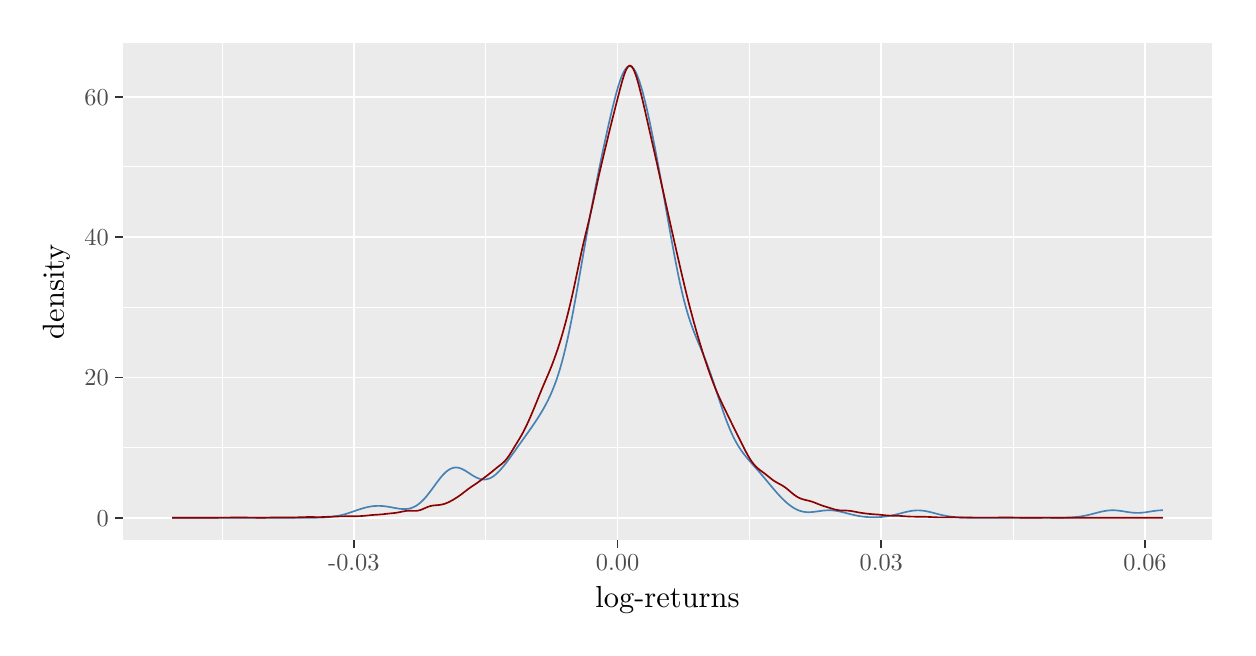
\begin{tikzpicture}[x=1pt,y=1pt]
\definecolor{fillColor}{RGB}{255,255,255}
\path[use as bounding box,fill=fillColor,fill opacity=0.00] (0,0) rectangle (433.62,216.81);
\begin{scope}
\path[clip] (  0.00,  0.00) rectangle (433.62,216.81);
\definecolor{drawColor}{RGB}{255,255,255}
\definecolor{fillColor}{RGB}{255,255,255}

\path[draw=drawColor,line width= 0.6pt,line join=round,line cap=round,fill=fillColor] (  0.00,  0.00) rectangle (433.62,216.81);
\end{scope}
\begin{scope}
\path[clip] ( 34.27, 31.53) rectangle (428.12,211.31);
\definecolor{fillColor}{gray}{0.92}

\path[fill=fillColor] ( 34.27, 31.53) rectangle (428.12,211.31);
\definecolor{drawColor}{RGB}{255,255,255}

\path[draw=drawColor,line width= 0.3pt,line join=round] ( 34.27, 65.06) --
	(428.12, 65.06);

\path[draw=drawColor,line width= 0.3pt,line join=round] ( 34.27,115.78) --
	(428.12,115.78);

\path[draw=drawColor,line width= 0.3pt,line join=round] ( 34.27,166.50) --
	(428.12,166.50);

\path[draw=drawColor,line width= 0.3pt,line join=round] ( 70.24, 31.53) --
	( 70.24,211.31);

\path[draw=drawColor,line width= 0.3pt,line join=round] (165.52, 31.53) --
	(165.52,211.31);

\path[draw=drawColor,line width= 0.3pt,line join=round] (260.81, 31.53) --
	(260.81,211.31);

\path[draw=drawColor,line width= 0.3pt,line join=round] (356.09, 31.53) --
	(356.09,211.31);

\path[draw=drawColor,line width= 0.6pt,line join=round] ( 34.27, 39.70) --
	(428.12, 39.70);

\path[draw=drawColor,line width= 0.6pt,line join=round] ( 34.27, 90.42) --
	(428.12, 90.42);

\path[draw=drawColor,line width= 0.6pt,line join=round] ( 34.27,141.14) --
	(428.12,141.14);

\path[draw=drawColor,line width= 0.6pt,line join=round] ( 34.27,191.86) --
	(428.12,191.86);

\path[draw=drawColor,line width= 0.6pt,line join=round] (117.88, 31.53) --
	(117.88,211.31);

\path[draw=drawColor,line width= 0.6pt,line join=round] (213.17, 31.53) --
	(213.17,211.31);

\path[draw=drawColor,line width= 0.6pt,line join=round] (308.45, 31.53) --
	(308.45,211.31);

\path[draw=drawColor,line width= 0.6pt,line join=round] (403.74, 31.53) --
	(403.74,211.31);
\definecolor{drawColor}{RGB}{70,130,180}

\path[draw=drawColor,line width= 0.6pt,line join=round] ( 52.17, 39.70) --
	( 52.87, 39.70) --
	( 53.57, 39.70) --
	( 54.27, 39.70) --
	( 54.97, 39.70) --
	( 55.67, 39.70) --
	( 56.37, 39.70) --
	( 57.07, 39.70) --
	( 57.78, 39.70) --
	( 58.48, 39.70) --
	( 59.18, 39.70) --
	( 59.88, 39.70) --
	( 60.58, 39.70) --
	( 61.28, 39.70) --
	( 61.98, 39.70) --
	( 62.68, 39.70) --
	( 63.38, 39.70) --
	( 64.08, 39.70) --
	( 64.78, 39.70) --
	( 65.48, 39.70) --
	( 66.18, 39.70) --
	( 66.88, 39.70) --
	( 67.59, 39.70) --
	( 68.29, 39.70) --
	( 68.99, 39.70) --
	( 69.69, 39.70) --
	( 70.39, 39.70) --
	( 71.09, 39.70) --
	( 71.79, 39.70) --
	( 72.49, 39.70) --
	( 73.19, 39.70) --
	( 73.89, 39.70) --
	( 74.59, 39.70) --
	( 75.29, 39.70) --
	( 75.99, 39.70) --
	( 76.69, 39.70) --
	( 77.39, 39.70) --
	( 78.10, 39.70) --
	( 78.80, 39.70) --
	( 79.50, 39.70) --
	( 80.20, 39.70) --
	( 80.90, 39.70) --
	( 81.60, 39.70) --
	( 82.30, 39.70) --
	( 83.00, 39.70) --
	( 83.70, 39.70) --
	( 84.40, 39.70) --
	( 85.10, 39.70) --
	( 85.80, 39.70) --
	( 86.50, 39.70) --
	( 87.20, 39.70) --
	( 87.90, 39.70) --
	( 88.61, 39.70) --
	( 89.31, 39.70) --
	( 90.01, 39.70) --
	( 90.71, 39.70) --
	( 91.41, 39.70) --
	( 92.11, 39.70) --
	( 92.81, 39.70) --
	( 93.51, 39.70) --
	( 94.21, 39.70) --
	( 94.91, 39.70) --
	( 95.61, 39.70) --
	( 96.31, 39.70) --
	( 97.01, 39.70) --
	( 97.71, 39.70) --
	( 98.42, 39.70) --
	( 99.12, 39.70) --
	( 99.82, 39.71) --
	(100.52, 39.71) --
	(101.22, 39.71) --
	(101.92, 39.71) --
	(102.62, 39.72) --
	(103.32, 39.73) --
	(104.02, 39.73) --
	(104.72, 39.75) --
	(105.42, 39.76) --
	(106.12, 39.79) --
	(106.82, 39.82) --
	(107.52, 39.85) --
	(108.22, 39.90) --
	(108.93, 39.95) --
	(109.63, 40.02) --
	(110.33, 40.11) --
	(111.03, 40.21) --
	(111.73, 40.33) --
	(112.43, 40.46) --
	(113.13, 40.62) --
	(113.83, 40.79) --
	(114.53, 40.98) --
	(115.23, 41.18) --
	(115.93, 41.40) --
	(116.63, 41.64) --
	(117.33, 41.88) --
	(118.03, 42.12) --
	(118.73, 42.36) --
	(119.44, 42.60) --
	(120.14, 42.83) --
	(120.84, 43.05) --
	(121.54, 43.26) --
	(122.24, 43.44) --
	(122.94, 43.60) --
	(123.64, 43.74) --
	(124.34, 43.85) --
	(125.04, 43.93) --
	(125.74, 43.98) --
	(126.44, 44.01) --
	(127.14, 44.01) --
	(127.84, 43.98) --
	(128.54, 43.92) --
	(129.24, 43.84) --
	(129.95, 43.75) --
	(130.65, 43.63) --
	(131.35, 43.51) --
	(132.05, 43.37) --
	(132.75, 43.24) --
	(133.45, 43.12) --
	(134.15, 43.01) --
	(134.85, 42.92) --
	(135.55, 42.87) --
	(136.25, 42.86) --
	(136.95, 42.90) --
	(137.65, 42.99) --
	(138.35, 43.15) --
	(139.05, 43.39) --
	(139.76, 43.71) --
	(140.46, 44.10) --
	(141.16, 44.59) --
	(141.86, 45.15) --
	(142.56, 45.79) --
	(143.26, 46.51) --
	(143.96, 47.30) --
	(144.66, 48.15) --
	(145.36, 49.06) --
	(146.06, 50.00) --
	(146.76, 50.96) --
	(147.46, 51.92) --
	(148.16, 52.86) --
	(148.86, 53.77) --
	(149.56, 54.63) --
	(150.27, 55.42) --
	(150.97, 56.12) --
	(151.67, 56.70) --
	(152.37, 57.18) --
	(153.07, 57.53) --
	(153.77, 57.76) --
	(154.47, 57.87) --
	(155.17, 57.86) --
	(155.87, 57.74) --
	(156.57, 57.50) --
	(157.27, 57.19) --
	(157.97, 56.81) --
	(158.67, 56.38) --
	(159.37, 55.93) --
	(160.07, 55.47) --
	(160.78, 55.02) --
	(161.48, 54.60) --
	(162.18, 54.24) --
	(162.88, 53.94) --
	(163.58, 53.71) --
	(164.28, 53.58) --
	(164.98, 53.53) --
	(165.68, 53.59) --
	(166.38, 53.75) --
	(167.08, 54.01) --
	(167.78, 54.38) --
	(168.48, 54.85) --
	(169.18, 55.41) --
	(169.88, 56.06) --
	(170.59, 56.78) --
	(171.29, 57.57) --
	(171.99, 58.41) --
	(172.69, 59.29) --
	(173.39, 60.22) --
	(174.09, 61.17) --
	(174.79, 62.14) --
	(175.49, 63.11) --
	(176.19, 64.09) --
	(176.89, 65.08) --
	(177.59, 66.06) --
	(178.29, 67.04) --
	(178.99, 68.02) --
	(179.69, 69.01) --
	(180.39, 69.99) --
	(181.10, 70.98) --
	(181.80, 71.98) --
	(182.50, 72.99) --
	(183.20, 74.02) --
	(183.90, 75.08) --
	(184.60, 76.16) --
	(185.30, 77.29) --
	(186.00, 78.46) --
	(186.70, 79.69) --
	(187.40, 80.99) --
	(188.10, 82.37) --
	(188.80, 83.85) --
	(189.50, 85.45) --
	(190.20, 87.18) --
	(190.90, 89.06) --
	(191.61, 91.13) --
	(192.31, 93.39) --
	(193.01, 95.84) --
	(193.71, 98.50) --
	(194.41,101.37) --
	(195.11,104.44) --
	(195.81,107.72) --
	(196.51,111.18) --
	(197.21,114.84) --
	(197.91,118.64) --
	(198.61,122.55) --
	(199.31,126.53) --
	(200.01,130.56) --
	(200.71,134.61) --
	(201.42,138.64) --
	(202.12,142.64) --
	(202.82,146.56) --
	(203.52,150.40) --
	(204.22,154.16) --
	(204.92,157.82) --
	(205.62,161.40) --
	(206.32,164.89) --
	(207.02,168.31) --
	(207.72,171.67) --
	(208.42,174.96) --
	(209.12,178.18) --
	(209.82,181.34) --
	(210.52,184.42) --
	(211.22,187.39) --
	(211.93,190.23) --
	(212.63,192.91) --
	(213.33,195.37) --
	(214.03,197.57) --
	(214.73,199.42) --
	(215.43,200.91) --
	(216.13,202.01) --
	(216.83,202.68) --
	(217.53,202.92) --
	(218.23,202.70) --
	(218.93,202.04) --
	(219.63,200.95) --
	(220.33,199.40) --
	(221.03,197.48) --
	(221.73,195.24) --
	(222.44,192.72) --
	(223.14,189.95) --
	(223.84,186.97) --
	(224.54,183.82) --
	(225.24,180.50) --
	(225.94,177.05) --
	(226.64,173.48) --
	(227.34,169.81) --
	(228.04,166.05) --
	(228.74,162.21) --
	(229.44,158.31) --
	(230.14,154.36) --
	(230.84,150.38) --
	(231.54,146.39) --
	(232.24,142.44) --
	(232.95,138.55) --
	(233.65,134.76) --
	(234.35,131.10) --
	(235.05,127.60) --
	(235.75,124.30) --
	(236.45,121.20) --
	(237.15,118.33) --
	(237.85,115.71) --
	(238.55,113.30) --
	(239.25,111.10) --
	(239.95,109.07) --
	(240.65,107.18) --
	(241.35,105.40) --
	(242.05,103.69) --
	(242.76,102.03) --
	(243.46,100.36) --
	(244.16, 98.65) --
	(244.86, 96.89) --
	(245.56, 95.06) --
	(246.26, 93.15) --
	(246.96, 91.17) --
	(247.66, 89.12) --
	(248.36, 87.01) --
	(249.06, 84.88) --
	(249.76, 82.74) --
	(250.46, 80.63) --
	(251.16, 78.56) --
	(251.86, 76.56) --
	(252.56, 74.65) --
	(253.27, 72.85) --
	(253.97, 71.16) --
	(254.67, 69.61) --
	(255.37, 68.18) --
	(256.07, 66.88) --
	(256.77, 65.68) --
	(257.47, 64.59) --
	(258.17, 63.58) --
	(258.87, 62.64) --
	(259.57, 61.76) --
	(260.27, 60.92) --
	(260.97, 60.11) --
	(261.67, 59.31) --
	(262.37, 58.53) --
	(263.07, 57.73) --
	(263.78, 56.94) --
	(264.48, 56.13) --
	(265.18, 55.31) --
	(265.88, 54.49) --
	(266.58, 53.65) --
	(267.28, 52.81) --
	(267.98, 51.97) --
	(268.68, 51.13) --
	(269.38, 50.30) --
	(270.08, 49.48) --
	(270.78, 48.68) --
	(271.48, 47.90) --
	(272.18, 47.16) --
	(272.88, 46.44) --
	(273.59, 45.77) --
	(274.29, 45.13) --
	(274.99, 44.55) --
	(275.69, 44.01) --
	(276.39, 43.53) --
	(277.09, 43.10) --
	(277.79, 42.73) --
	(278.49, 42.42) --
	(279.19, 42.18) --
	(279.89, 41.99) --
	(280.59, 41.85) --
	(281.29, 41.77) --
	(281.99, 41.73) --
	(282.69, 41.74) --
	(283.39, 41.78) --
	(284.10, 41.85) --
	(284.80, 41.94) --
	(285.50, 42.03) --
	(286.20, 42.13) --
	(286.90, 42.23) --
	(287.60, 42.31) --
	(288.30, 42.37) --
	(289.00, 42.41) --
	(289.70, 42.42) --
	(290.40, 42.40) --
	(291.10, 42.35) --
	(291.80, 42.27) --
	(292.50, 42.16) --
	(293.20, 42.03) --
	(293.90, 41.87) --
	(294.61, 41.71) --
	(295.31, 41.53) --
	(296.01, 41.34) --
	(296.71, 41.16) --
	(297.41, 40.98) --
	(298.11, 40.81) --
	(298.81, 40.65) --
	(299.51, 40.50) --
	(300.21, 40.37) --
	(300.91, 40.25) --
	(301.61, 40.16) --
	(302.31, 40.08) --
	(303.01, 40.01) --
	(303.71, 39.96) --
	(304.41, 39.93) --
	(305.12, 39.90) --
	(305.82, 39.90) --
	(306.52, 39.90) --
	(307.22, 39.93) --
	(307.92, 39.97) --
	(308.62, 40.02) --
	(309.32, 40.09) --
	(310.02, 40.17) --
	(310.72, 40.27) --
	(311.42, 40.39) --
	(312.12, 40.52) --
	(312.82, 40.67) --
	(313.52, 40.83) --
	(314.22, 41.00) --
	(314.93, 41.18) --
	(315.63, 41.36) --
	(316.33, 41.55) --
	(317.03, 41.73) --
	(317.73, 41.89) --
	(318.43, 42.04) --
	(319.13, 42.17) --
	(319.83, 42.27) --
	(320.53, 42.34) --
	(321.23, 42.38) --
	(321.93, 42.38) --
	(322.63, 42.36) --
	(323.33, 42.29) --
	(324.03, 42.20) --
	(324.73, 42.08) --
	(325.44, 41.93) --
	(326.14, 41.77) --
	(326.84, 41.60) --
	(327.54, 41.41) --
	(328.24, 41.23) --
	(328.94, 41.05) --
	(329.64, 40.87) --
	(330.34, 40.70) --
	(331.04, 40.55) --
	(331.74, 40.41) --
	(332.44, 40.29) --
	(333.14, 40.18) --
	(333.84, 40.09) --
	(334.54, 40.01) --
	(335.24, 39.94) --
	(335.95, 39.89) --
	(336.65, 39.84) --
	(337.35, 39.81) --
	(338.05, 39.78) --
	(338.75, 39.76) --
	(339.45, 39.75) --
	(340.15, 39.73) --
	(340.85, 39.72) --
	(341.55, 39.72) --
	(342.25, 39.71) --
	(342.95, 39.71) --
	(343.65, 39.71) --
	(344.35, 39.71) --
	(345.05, 39.70) --
	(345.76, 39.70) --
	(346.46, 39.70) --
	(347.16, 39.70) --
	(347.86, 39.70) --
	(348.56, 39.70) --
	(349.26, 39.70) --
	(349.96, 39.70) --
	(350.66, 39.70) --
	(351.36, 39.70) --
	(352.06, 39.70) --
	(352.76, 39.70) --
	(353.46, 39.70) --
	(354.16, 39.70) --
	(354.86, 39.70) --
	(355.56, 39.70) --
	(356.27, 39.70) --
	(356.97, 39.70) --
	(357.67, 39.70) --
	(358.37, 39.70) --
	(359.07, 39.70) --
	(359.77, 39.70) --
	(360.47, 39.70) --
	(361.17, 39.70) --
	(361.87, 39.70) --
	(362.57, 39.70) --
	(363.27, 39.70) --
	(363.97, 39.70) --
	(364.67, 39.70) --
	(365.37, 39.70) --
	(366.07, 39.70) --
	(366.78, 39.70) --
	(367.48, 39.70) --
	(368.18, 39.70) --
	(368.88, 39.71) --
	(369.58, 39.71) --
	(370.28, 39.71) --
	(370.98, 39.71) --
	(371.68, 39.72) --
	(372.38, 39.72) --
	(373.08, 39.73) --
	(373.78, 39.74) --
	(374.48, 39.75) --
	(375.18, 39.77) --
	(375.88, 39.80) --
	(376.58, 39.83) --
	(377.29, 39.87) --
	(377.99, 39.92) --
	(378.69, 39.98) --
	(379.39, 40.06) --
	(380.09, 40.14) --
	(380.79, 40.25) --
	(381.49, 40.36) --
	(382.19, 40.50) --
	(382.89, 40.64) --
	(383.59, 40.81) --
	(384.29, 40.98) --
	(384.99, 41.16) --
	(385.69, 41.34) --
	(386.39, 41.53) --
	(387.10, 41.71) --
	(387.80, 41.88) --
	(388.50, 42.03) --
	(389.20, 42.16) --
	(389.90, 42.27) --
	(390.60, 42.35) --
	(391.30, 42.40) --
	(392.00, 42.42) --
	(392.70, 42.41) --
	(393.40, 42.37) --
	(394.10, 42.30) --
	(394.80, 42.21) --
	(395.50, 42.11) --
	(396.20, 42.00) --
	(396.90, 41.88) --
	(397.61, 41.77) --
	(398.31, 41.67) --
	(399.01, 41.59) --
	(399.71, 41.52) --
	(400.41, 41.49) --
	(401.11, 41.48) --
	(401.81, 41.50) --
	(402.51, 41.54) --
	(403.21, 41.61) --
	(403.91, 41.69) --
	(404.61, 41.80) --
	(405.31, 41.91) --
	(406.01, 42.02) --
	(406.71, 42.13) --
	(407.41, 42.23) --
	(408.12, 42.32) --
	(408.82, 42.38) --
	(409.52, 42.41) --
	(410.22, 42.42);
\definecolor{drawColor}{RGB}{139,0,0}

\path[draw=drawColor,line width= 0.6pt,line join=round] ( 52.17, 39.73) --
	( 52.87, 39.73) --
	( 53.57, 39.73) --
	( 54.27, 39.72) --
	( 54.97, 39.72) --
	( 55.67, 39.72) --
	( 56.37, 39.72) --
	( 57.07, 39.72) --
	( 57.78, 39.72) --
	( 58.48, 39.73) --
	( 59.18, 39.73) --
	( 59.88, 39.73) --
	( 60.58, 39.73) --
	( 61.28, 39.73) --
	( 61.98, 39.72) --
	( 62.68, 39.72) --
	( 63.38, 39.71) --
	( 64.08, 39.71) --
	( 64.78, 39.71) --
	( 65.48, 39.71) --
	( 66.18, 39.71) --
	( 66.88, 39.72) --
	( 67.59, 39.73) --
	( 68.29, 39.74) --
	( 68.99, 39.75) --
	( 69.69, 39.76) --
	( 70.39, 39.77) --
	( 71.09, 39.77) --
	( 71.79, 39.78) --
	( 72.49, 39.78) --
	( 73.19, 39.78) --
	( 73.89, 39.79) --
	( 74.59, 39.80) --
	( 75.29, 39.80) --
	( 75.99, 39.81) --
	( 76.69, 39.81) --
	( 77.39, 39.80) --
	( 78.10, 39.80) --
	( 78.80, 39.79) --
	( 79.50, 39.78) --
	( 80.20, 39.78) --
	( 80.90, 39.77) --
	( 81.60, 39.76) --
	( 82.30, 39.75) --
	( 83.00, 39.74) --
	( 83.70, 39.74) --
	( 84.40, 39.73) --
	( 85.10, 39.74) --
	( 85.80, 39.74) --
	( 86.50, 39.76) --
	( 87.20, 39.77) --
	( 87.90, 39.79) --
	( 88.61, 39.81) --
	( 89.31, 39.82) --
	( 90.01, 39.82) --
	( 90.71, 39.82) --
	( 91.41, 39.82) --
	( 92.11, 39.81) --
	( 92.81, 39.80) --
	( 93.51, 39.80) --
	( 94.21, 39.80) --
	( 94.91, 39.81) --
	( 95.61, 39.82) --
	( 96.31, 39.83) --
	( 97.01, 39.85) --
	( 97.71, 39.87) --
	( 98.42, 39.90) --
	( 99.12, 39.92) --
	( 99.82, 39.94) --
	(100.52, 39.96) --
	(101.22, 39.98) --
	(101.92, 39.98) --
	(102.62, 39.98) --
	(103.32, 39.97) --
	(104.02, 39.95) --
	(104.72, 39.94) --
	(105.42, 39.95) --
	(106.12, 39.96) --
	(106.82, 39.98) --
	(107.52, 40.02) --
	(108.22, 40.06) --
	(108.93, 40.09) --
	(109.63, 40.12) --
	(110.33, 40.15) --
	(111.03, 40.17) --
	(111.73, 40.18) --
	(112.43, 40.20) --
	(113.13, 40.21) --
	(113.83, 40.22) --
	(114.53, 40.24) --
	(115.23, 40.25) --
	(115.93, 40.26) --
	(116.63, 40.26) --
	(117.33, 40.26) --
	(118.03, 40.26) --
	(118.73, 40.27) --
	(119.44, 40.29) --
	(120.14, 40.31) --
	(120.84, 40.36) --
	(121.54, 40.41) --
	(122.24, 40.48) --
	(122.94, 40.55) --
	(123.64, 40.62) --
	(124.34, 40.69) --
	(125.04, 40.75) --
	(125.74, 40.79) --
	(126.44, 40.83) --
	(127.14, 40.88) --
	(127.84, 40.94) --
	(128.54, 41.01) --
	(129.24, 41.09) --
	(129.95, 41.17) --
	(130.65, 41.25) --
	(131.35, 41.32) --
	(132.05, 41.39) --
	(132.75, 41.46) --
	(133.45, 41.56) --
	(134.15, 41.69) --
	(134.85, 41.83) --
	(135.55, 41.98) --
	(136.25, 42.11) --
	(136.95, 42.20) --
	(137.65, 42.24) --
	(138.35, 42.24) --
	(139.05, 42.21) --
	(139.76, 42.19) --
	(140.46, 42.22) --
	(141.16, 42.32) --
	(141.86, 42.50) --
	(142.56, 42.76) --
	(143.26, 43.07) --
	(143.96, 43.38) --
	(144.66, 43.67) --
	(145.36, 43.91) --
	(146.06, 44.07) --
	(146.76, 44.17) --
	(147.46, 44.24) --
	(148.16, 44.29) --
	(148.86, 44.37) --
	(149.56, 44.48) --
	(150.27, 44.65) --
	(150.97, 44.87) --
	(151.67, 45.15) --
	(152.37, 45.48) --
	(153.07, 45.85) --
	(153.77, 46.24) --
	(154.47, 46.67) --
	(155.17, 47.11) --
	(155.87, 47.59) --
	(156.57, 48.09) --
	(157.27, 48.62) --
	(157.97, 49.16) --
	(158.67, 49.71) --
	(159.37, 50.23) --
	(160.07, 50.73) --
	(160.78, 51.20) --
	(161.48, 51.67) --
	(162.18, 52.14) --
	(162.88, 52.64) --
	(163.58, 53.15) --
	(164.28, 53.67) --
	(164.98, 54.20) --
	(165.68, 54.72) --
	(166.38, 55.25) --
	(167.08, 55.80) --
	(167.78, 56.36) --
	(168.48, 56.94) --
	(169.18, 57.51) --
	(169.88, 58.07) --
	(170.59, 58.61) --
	(171.29, 59.17) --
	(171.99, 59.78) --
	(172.69, 60.51) --
	(173.39, 61.38) --
	(174.09, 62.39) --
	(174.79, 63.50) --
	(175.49, 64.65) --
	(176.19, 65.80) --
	(176.89, 66.95) --
	(177.59, 68.09) --
	(178.29, 69.28) --
	(178.99, 70.55) --
	(179.69, 71.90) --
	(180.39, 73.36) --
	(181.10, 74.89) --
	(181.80, 76.49) --
	(182.50, 78.14) --
	(183.20, 79.83) --
	(183.90, 81.54) --
	(184.60, 83.28) --
	(185.30, 85.00) --
	(186.00, 86.69) --
	(186.70, 88.35) --
	(187.40, 89.97) --
	(188.10, 91.60) --
	(188.80, 93.28) --
	(189.50, 95.05) --
	(190.20, 96.90) --
	(190.90, 98.86) --
	(191.61,100.93) --
	(192.31,103.11) --
	(193.01,105.41) --
	(193.71,107.85) --
	(194.41,110.42) --
	(195.11,113.12) --
	(195.81,115.95) --
	(196.51,118.93) --
	(197.21,122.05) --
	(197.91,125.30) --
	(198.61,128.64) --
	(199.31,132.00) --
	(200.01,135.28) --
	(200.71,138.41) --
	(201.42,141.40) --
	(202.12,144.29) --
	(202.82,147.18) --
	(203.52,150.19) --
	(204.22,153.33) --
	(204.92,156.57) --
	(205.62,159.82) --
	(206.32,163.01) --
	(207.02,166.07) --
	(207.72,169.04) --
	(208.42,171.96) --
	(209.12,174.86) --
	(209.82,177.78) --
	(210.52,180.68) --
	(211.22,183.53) --
	(211.93,186.33) --
	(212.63,189.09) --
	(213.33,191.82) --
	(214.03,194.52) --
	(214.73,197.11) --
	(215.43,199.46) --
	(216.13,201.37) --
	(216.83,202.65) --
	(217.53,203.14) --
	(218.23,202.82) --
	(218.93,201.74) --
	(219.63,200.03) --
	(220.33,197.82) --
	(221.03,195.27) --
	(221.73,192.47) --
	(222.44,189.53) --
	(223.14,186.50) --
	(223.84,183.42) --
	(224.54,180.33) --
	(225.24,177.23) --
	(225.94,174.14) --
	(226.64,171.04) --
	(227.34,167.92) --
	(228.04,164.80) --
	(228.74,161.65) --
	(229.44,158.50) --
	(230.14,155.34) --
	(230.84,152.18) --
	(231.54,149.02) --
	(232.24,145.85) --
	(232.95,142.70) --
	(233.65,139.57) --
	(234.35,136.47) --
	(235.05,133.39) --
	(235.75,130.34) --
	(236.45,127.32) --
	(237.15,124.35) --
	(237.85,121.44) --
	(238.55,118.62) --
	(239.25,115.89) --
	(239.95,113.24) --
	(240.65,110.66) --
	(241.35,108.15) --
	(242.05,105.69) --
	(242.76,103.29) --
	(243.46,100.96) --
	(244.16, 98.71) --
	(244.86, 96.54) --
	(245.56, 94.44) --
	(246.26, 92.43) --
	(246.96, 90.48) --
	(247.66, 88.61) --
	(248.36, 86.82) --
	(249.06, 85.13) --
	(249.76, 83.52) --
	(250.46, 81.99) --
	(251.16, 80.51) --
	(251.86, 79.06) --
	(252.56, 77.62) --
	(253.27, 76.18) --
	(253.97, 74.73) --
	(254.67, 73.30) --
	(255.37, 71.89) --
	(256.07, 70.49) --
	(256.77, 69.09) --
	(257.47, 67.68) --
	(258.17, 66.26) --
	(258.87, 64.86) --
	(259.57, 63.49) --
	(260.27, 62.21) --
	(260.97, 61.03) --
	(261.67, 59.98) --
	(262.37, 59.07) --
	(263.07, 58.28) --
	(263.78, 57.62) --
	(264.48, 57.04) --
	(265.18, 56.52) --
	(265.88, 56.01) --
	(266.58, 55.48) --
	(267.28, 54.92) --
	(267.98, 54.36) --
	(268.68, 53.80) --
	(269.38, 53.27) --
	(270.08, 52.81) --
	(270.78, 52.40) --
	(271.48, 52.02) --
	(272.18, 51.65) --
	(272.88, 51.24) --
	(273.59, 50.78) --
	(274.29, 50.25) --
	(274.99, 49.66) --
	(275.69, 49.06) --
	(276.39, 48.47) --
	(277.09, 47.92) --
	(277.79, 47.44) --
	(278.49, 47.03) --
	(279.19, 46.71) --
	(279.89, 46.45) --
	(280.59, 46.26) --
	(281.29, 46.09) --
	(281.99, 45.93) --
	(282.69, 45.75) --
	(283.39, 45.54) --
	(284.10, 45.29) --
	(284.80, 45.01) --
	(285.50, 44.73) --
	(286.20, 44.46) --
	(286.90, 44.20) --
	(287.60, 43.96) --
	(288.30, 43.74) --
	(289.00, 43.53) --
	(289.70, 43.31) --
	(290.40, 43.09) --
	(291.10, 42.87) --
	(291.80, 42.68) --
	(292.50, 42.52) --
	(293.20, 42.42) --
	(293.90, 42.36) --
	(294.61, 42.34) --
	(295.31, 42.33) --
	(296.01, 42.31) --
	(296.71, 42.26) --
	(297.41, 42.17) --
	(298.11, 42.06) --
	(298.81, 41.92) --
	(299.51, 41.78) --
	(300.21, 41.65) --
	(300.91, 41.53) --
	(301.61, 41.43) --
	(302.31, 41.33) --
	(303.01, 41.24) --
	(303.71, 41.16) --
	(304.41, 41.08) --
	(305.12, 41.02) --
	(305.82, 40.97) --
	(306.52, 40.93) --
	(307.22, 40.88) --
	(307.92, 40.82) --
	(308.62, 40.74) --
	(309.32, 40.66) --
	(310.02, 40.59) --
	(310.72, 40.53) --
	(311.42, 40.49) --
	(312.12, 40.47) --
	(312.82, 40.47) --
	(313.52, 40.46) --
	(314.22, 40.45) --
	(314.93, 40.41) --
	(315.63, 40.36) --
	(316.33, 40.30) --
	(317.03, 40.25) --
	(317.73, 40.20) --
	(318.43, 40.16) --
	(319.13, 40.14) --
	(319.83, 40.12) --
	(320.53, 40.11) --
	(321.23, 40.10) --
	(321.93, 40.09) --
	(322.63, 40.09) --
	(323.33, 40.08) --
	(324.03, 40.06) --
	(324.73, 40.05) --
	(325.44, 40.02) --
	(326.14, 39.99) --
	(326.84, 39.95) --
	(327.54, 39.92) --
	(328.24, 39.89) --
	(328.94, 39.86) --
	(329.64, 39.85) --
	(330.34, 39.85) --
	(331.04, 39.86) --
	(331.74, 39.87) --
	(332.44, 39.88) --
	(333.14, 39.89) --
	(333.84, 39.89) --
	(334.54, 39.89) --
	(335.24, 39.87) --
	(335.95, 39.86) --
	(336.65, 39.84) --
	(337.35, 39.83) --
	(338.05, 39.82) --
	(338.75, 39.82) --
	(339.45, 39.81) --
	(340.15, 39.80) --
	(340.85, 39.79) --
	(341.55, 39.78) --
	(342.25, 39.77) --
	(342.95, 39.76) --
	(343.65, 39.76) --
	(344.35, 39.75) --
	(345.05, 39.75) --
	(345.76, 39.75) --
	(346.46, 39.75) --
	(347.16, 39.76) --
	(347.86, 39.76) --
	(348.56, 39.77) --
	(349.26, 39.77) --
	(349.96, 39.78) --
	(350.66, 39.78) --
	(351.36, 39.79) --
	(352.06, 39.79) --
	(352.76, 39.80) --
	(353.46, 39.80) --
	(354.16, 39.80) --
	(354.86, 39.80) --
	(355.56, 39.79) --
	(356.27, 39.78) --
	(356.97, 39.77) --
	(357.67, 39.76) --
	(358.37, 39.75) --
	(359.07, 39.74) --
	(359.77, 39.73) --
	(360.47, 39.73) --
	(361.17, 39.72) --
	(361.87, 39.71) --
	(362.57, 39.71) --
	(363.27, 39.71) --
	(363.97, 39.72) --
	(364.67, 39.72) --
	(365.37, 39.73) --
	(366.07, 39.74) --
	(366.78, 39.75) --
	(367.48, 39.76) --
	(368.18, 39.76) --
	(368.88, 39.76) --
	(369.58, 39.75) --
	(370.28, 39.74) --
	(370.98, 39.73) --
	(371.68, 39.72) --
	(372.38, 39.72) --
	(373.08, 39.71) --
	(373.78, 39.71) --
	(374.48, 39.70) --
	(375.18, 39.70) --
	(375.88, 39.70) --
	(376.58, 39.70) --
	(377.29, 39.70) --
	(377.99, 39.70) --
	(378.69, 39.70) --
	(379.39, 39.70) --
	(380.09, 39.70) --
	(380.79, 39.70) --
	(381.49, 39.70) --
	(382.19, 39.70) --
	(382.89, 39.70) --
	(383.59, 39.70) --
	(384.29, 39.70) --
	(384.99, 39.70) --
	(385.69, 39.70) --
	(386.39, 39.70) --
	(387.10, 39.70) --
	(387.80, 39.70) --
	(388.50, 39.70) --
	(389.20, 39.70) --
	(389.90, 39.70) --
	(390.60, 39.70) --
	(391.30, 39.70) --
	(392.00, 39.70) --
	(392.70, 39.70) --
	(393.40, 39.70) --
	(394.10, 39.70) --
	(394.80, 39.70) --
	(395.50, 39.70) --
	(396.20, 39.70) --
	(396.90, 39.70) --
	(397.61, 39.70) --
	(398.31, 39.70) --
	(399.01, 39.70) --
	(399.71, 39.70) --
	(400.41, 39.70) --
	(401.11, 39.70) --
	(401.81, 39.70) --
	(402.51, 39.70) --
	(403.21, 39.70) --
	(403.91, 39.70) --
	(404.61, 39.70) --
	(405.31, 39.70) --
	(406.01, 39.70) --
	(406.71, 39.70) --
	(407.41, 39.70) --
	(408.12, 39.70) --
	(408.82, 39.70) --
	(409.52, 39.70) --
	(410.22, 39.70);
\end{scope}
\begin{scope}
\path[clip] (  0.00,  0.00) rectangle (433.62,216.81);
\definecolor{drawColor}{gray}{0.30}

\node[text=drawColor,anchor=base east,inner sep=0pt, outer sep=0pt, scale=  0.88] at ( 29.32, 36.67) {0};

\node[text=drawColor,anchor=base east,inner sep=0pt, outer sep=0pt, scale=  0.88] at ( 29.32, 87.39) {20};

\node[text=drawColor,anchor=base east,inner sep=0pt, outer sep=0pt, scale=  0.88] at ( 29.32,138.11) {40};

\node[text=drawColor,anchor=base east,inner sep=0pt, outer sep=0pt, scale=  0.88] at ( 29.32,188.83) {60};
\end{scope}
\begin{scope}
\path[clip] (  0.00,  0.00) rectangle (433.62,216.81);
\definecolor{drawColor}{gray}{0.20}

\path[draw=drawColor,line width= 0.6pt,line join=round] ( 31.52, 39.70) --
	( 34.27, 39.70);

\path[draw=drawColor,line width= 0.6pt,line join=round] ( 31.52, 90.42) --
	( 34.27, 90.42);

\path[draw=drawColor,line width= 0.6pt,line join=round] ( 31.52,141.14) --
	( 34.27,141.14);

\path[draw=drawColor,line width= 0.6pt,line join=round] ( 31.52,191.86) --
	( 34.27,191.86);
\end{scope}
\begin{scope}
\path[clip] (  0.00,  0.00) rectangle (433.62,216.81);
\definecolor{drawColor}{gray}{0.20}

\path[draw=drawColor,line width= 0.6pt,line join=round] (117.88, 28.78) --
	(117.88, 31.53);

\path[draw=drawColor,line width= 0.6pt,line join=round] (213.17, 28.78) --
	(213.17, 31.53);

\path[draw=drawColor,line width= 0.6pt,line join=round] (308.45, 28.78) --
	(308.45, 31.53);

\path[draw=drawColor,line width= 0.6pt,line join=round] (403.74, 28.78) --
	(403.74, 31.53);
\end{scope}
\begin{scope}
\path[clip] (  0.00,  0.00) rectangle (433.62,216.81);
\definecolor{drawColor}{gray}{0.30}

\node[text=drawColor,anchor=base,inner sep=0pt, outer sep=0pt, scale=  0.88] at (117.88, 20.52) {-0.03};

\node[text=drawColor,anchor=base,inner sep=0pt, outer sep=0pt, scale=  0.88] at (213.17, 20.52) {0.00};

\node[text=drawColor,anchor=base,inner sep=0pt, outer sep=0pt, scale=  0.88] at (308.45, 20.52) {0.03};

\node[text=drawColor,anchor=base,inner sep=0pt, outer sep=0pt, scale=  0.88] at (403.74, 20.52) {0.06};
\end{scope}
\begin{scope}
\path[clip] (  0.00,  0.00) rectangle (433.62,216.81);
\definecolor{drawColor}{RGB}{0,0,0}

\node[text=drawColor,anchor=base,inner sep=0pt, outer sep=0pt, scale=  1.10] at (231.19,  7.44) {log-returns};
\end{scope}
\begin{scope}
\path[clip] (  0.00,  0.00) rectangle (433.62,216.81);
\definecolor{drawColor}{RGB}{0,0,0}

\node[text=drawColor,rotate= 90.00,anchor=base,inner sep=0pt, outer sep=0pt, scale=  1.10] at ( 13.08,121.42) {density};
\end{scope}
\end{tikzpicture}

  \caption{Historical and HSV related Apple stock Log-returns distribution in the risk-averse world}
  \floatfoot{The above blue density curve is constructed over the historical data of the Apple share of stock price evolution from 18th May 2017 to 18th May 2018. while the red curve is constructed from time-series genereated by the function \textit{hsv\_ts} taking the risk-averse parameters \ref{eq:methodology:arg:heston:riskaverse} as arguments.
  }
  \label{p:methodology:density:aapl:heston:riskaverse}
\end{figure}

Consequently, the set \ref{eq:methodology:arg:heston:riskaverse} is the one I will use together with the \textit{hsv\_ts()} function whenever I have to compute time series using the HSV model within the real world constraints for the purpose of that master thesis.


















\begin{appendices}
\chapter{R functions catalogue}
\label{cha:r}


For this master thesis, I created two R packages to help me in the analysis and in the related experiments. These packages are available, under open-source software license, through my GitHub account. Names are ”Random walk”  (https://github.com/AnthonyTedde/RandomWalk) and ”Stock price simulator” (https://github.com/AnthonyTedde/StockPriceSimulator).

The R package ”Random walk” contains functions that simulate time-discretized Brownian motions. It is widely used inside ”Stock price simulator”, mainly to add noise in the simulation of stock price time series. 

Unlike "Random walk", the package "Stock price simulator" is more multipurpose. The algorithms I developed inside range from the simulation of stock price path to the computation of option fair price and include hedging strategies, Greeks computation, Itô's approximation, characteristic functions and so on.

\Cref{sec:r:time} describes the functions inside the ”Stock price simulator” package that simulate time series by using a time discretization approximation.

\section{Time series simulation}
\label{sec:r:time}





%%%%%%%%%%%%%%%%%%%%%%%%%%%%%%%%%%%%%%%%%%%%%%%%%%%%%%%%%%%%%%
% GBM
%%%%%%%%%%%%%%%%%%%%%%%%%%%%%%%%%%%%%%%%%%%%%%%%%%%%%%%%%%%%%%
\subsection{Geometric Brownian motion}
\label{sub:r:time:geometric}

Based on \cref{eq:underlying:geometric:closed}, this function provides one possible path of a time-discretized version of the geometric Brownian motion.
It outputs a R data.frame comprised of two columns, namely "time\_periods" and "stock\_price\_path", which respectively denotes the period expressed in year and the corresponding value of the stock at that time.

\subsubsection*{function}

\begin{Schunk}
\begin{Sinput}
> sstock(initial_stock_price, time_to_maturity, 
        seed, scale, sigma, alpha)
\end{Sinput}
\end{Schunk}

\subsubsection*{Arguments}

\begin{tabularx}{\textwidth}{lX}
  initial\_stock\_price & Price of the stock at time zero.\\
  time\_to\_maturity & Duration of the simulation, expressed in year.\\
  seed & Parameter that fixes initial value of the pseudo random number generation in order to get reproducible experiment. \\
  scale & Number of time steps. For instance scale = 365 would mean daily measurement.\\
  sigma & Annualized volatility rate. \\
  alpha & Annualized drift rate.
\end{tabularx}

\subsubsection*{examples}
\label{sec:r:time:geometric:ex}

\begin{Schunk}
\begin{Sinput}
> s <- sstock(initial_stock_price = 100,
        time_to_maturity = 1,
        seed = 1,
        scale = 52,
        sigma = .2,
        alpha = .15)
\end{Sinput}
\end{Schunk}


\begin{Schunk}
\begin{Sinput}
> print(s)
\end{Sinput}
\end{Schunk}

\begin{table}[H]
\begin{tabular}{cc}
  \hline
 time\_periods (Year) & stock\_price\_path \\ 
  \hline
 0.00 & 100.00 \\ 
 0.02 & 98.52 \\ 
 0.04 & 99.27 \\ 
 0.06 & 97.24 \\ 
 0.08 & 101.90 \\ 
 \vdots & \vdots \\
 0.88 & 122.33 \\ 
 0.90 & 123.88 \\ 
 0.92 & 126.87 \\ 
 0.94 & 126.79 \\ 
 0.96 & 130.25 \\ 
 0.98 & 132.03 \\ 
 1.00 & 130.13 \\ 
   \hline
\end{tabular}
\caption{A sample of time-discretized geometric Brownian motion}
\end{table}





%%%%%%%%%%%%%%%%%%%%%%%%%%%%%%%%%%%%%%%%%%%%%%%%%%%%%%%%%%%%%%
% Merton
%%%%%%%%%%%%%%%%%%%%%%%%%%%%%%%%%%%%%%%%%%%%%%%%%%%%%%%%%%%%%%
\subsection{Merton Mixed jump-diffusion}
\label{sub:r:time:merton}

Based on \cref{eq:other:merton:pde}, this function provides one possible path of a time-discretized version of the Merton Mixed jump-diffusion model.
It outputs a R data.frame comprised of three columns. 
There are "time\_periods" ,"stock\_price\_path" which respectively denotes the period expressed in year and the corresponding values of the stock at that time.
In addition, the variable "grp" stand for "group" and allows to regroup the time series by jumps. Hunder the hood, a number, which is initialized to 0, is incremented as soon as a jump occurs, in this way, a whole series with the same number means that no jump occurred during its course.

\subsubsection*{function}

\begin{Schunk}
\begin{Sinput}
> sstock_jump(initial_stock_price, time_to_maturity, 
        seed, scale, sigma, alpha, lambda, jumps_intensity_parameters)
\end{Sinput}
\end{Schunk}

\subsubsection*{Arguments}

\begin{tabularx}{\textwidth}{lX}
  initial\_stock\_price & Price of the stock at time zero.\\
  time\_to\_maturity & Duration of the simulation, expressed in year.\\
  seed & Parameter that fixes initial value of the pseudo random number generation in order to get reproducible experiment. \\
  scale & Number of time steps. For instance scale = 365 would mean daily measurement.\\
  sigma & Annualized volatility rate. \\
  alpha & Annualized drift rate.\\
  lambda & Annualized jump frequency. \\
  jumps\_intensity\_parameters & List containing the parameters of the jump intensity. 
\end{tabularx}

\subsubsection*{examples}
\label{sec:r:time:geometric:ex}

\begin{Schunk}
\begin{Sinput}
> s <- sstock_jump(initial_stock_price = 100,
                  time_to_maturity = 1,
                  seed = 1,
                  scale = 52,
                  sigma = .2,
                  alpha = .15,
                  lambda = 5,
                  jumps_intensity_parameters = list(mean = .15, sd = .2))
\end{Sinput}
\end{Schunk}


\begin{Schunk}
\begin{Sinput}
> print(s)
\end{Sinput}
\end{Schunk}

\begin{table}[ht]
\centering
\begin{tabular}{lll}
  \hline
 time\_periods & stock\_price\_path &  grp \\ 
  \hline
   0.00 &100.00 &  0 \\ 
   0.02 &96.78  &  0 \\ 
   0.04 &95.80  &  0 \\ 
   0.06 &92.18  &  0 \\ 
   0.08 &94.89  &  0 \\ 
   0.10 &94.30  &  0 \\ 
   0.12 &90.78  &  0 \\ 
   0.13 &102.05 &  1 \\ 
 \vdots & \vdots & \vdots \\
 0.96 &55.02  &  3 \\ 
 0.98 &54.78  &  3 \\ 
 1.00 &53.04  &  3 \\ 
   \hline
\end{tabular}
\caption{A sample of time-discretized Merton Mixed jump-diffusion}
\end{table}





%%%%%%%%%%%%%%%%%%%%%%%%%%%%%%%%%%%%%%%%%%%%%%%%%%%%%%%%%%%%%%
% Heston
%%%%%%%%%%%%%%%%%%%%%%%%%%%%%%%%%%%%%%%%%%%%%%%%%%%%%%%%%%%%%%
\subsection{Heston stochastic volatility}
\label{sub:r:time:heston}

Based on \cref{eq:other:hsvvol,eq:other:hsvstock,eq:other:rho}, this function provides one possible path of a time-discretized version of the Heston stochastic volatility model.
It outputs a R data.frame comprised of five columns. 
There are "time\_periods" ,"stock\_price\_path" and "CIR", which respectively denotes the period expressed in year the corresponding values of the stock and of the volatility at that time.
In addition, the two more variables ”B1” and ”B2” stand for the Brownian motions that bring the noise in both stochastic processes $S(t)$ and $V(t)$.

\subsubsection*{function}

\begin{Schunk}
\begin{Sinput}
> heston(initial_stock_price, initial_volatility, time_to_maturity, 
        seed, scale, alpha, rho, kappa, theta, sigma)
\end{Sinput}
\end{Schunk}

\subsubsection*{Arguments}

\begin{tabularx}{\textwidth}{lX}
  initial\_stock\_price & Price of the stock at time zero.\\
  initial\_volatility & Volatility of the stock at time zero.\\
  time\_to\_maturity & Duration of the simulation, expressed in year.\\
  seed & Parameter that fixes initial value of the pseudo random number generation in order to get reproducible experiment. \\
  scale & Number of time steps. For instance scale = 365 would mean daily measurement.\\
  alpha & Annualized drift rate. \\
  rho & Correlation between the Stock price and volatility processes.\\
  kappa & Mean-reversion speed. \\
  theta & Volatility's long-run mean. \\
  sigma & Volatility of the volatility. 
\end{tabularx}

\subsubsection*{examples}
\label{sec:r:time:geometric:ex}

\begin{Schunk}
\begin{Sinput}
> s <- heston(initial_stock_price = 100,
             initial_volatility = .2,
             time_to_maturity = 1,
             seed = 1,
             scale = 52,
             alpha = .15,
             rho = -.8,
             kappa = 2,
             theta = .2,
             sigma = .1)
\end{Sinput}
\end{Schunk}


\begin{Schunk}
\begin{Sinput}
> print(s)
\end{Sinput}
\end{Schunk}

\begin{table}[H]
\centering
\begin{tabular}{lllll}
  \hline
 time\_periods & stock\_price\_path & B1 & B2 & CIR \\ 
  \hline
  0.00 & 100.00 & 0.00 & 0.00 & 0.20 \\ 
  0.02 & 96.40 & -0.09 & 0.10 & 0.20 \\ 
  0.04 & 97.79 & -0.06 & -0.02 & 0.20 \\ 
  0.06 & 93.02 & -0.18 & 0.20 & 0.21 \\ 
  0.08 & 102.68 & 0.04 & 0.18 & 0.21 \\ 
  \vdots &\vdots &\vdots &\vdots &\vdots\\
  0.92 & 142.21 & 0.59 & 0.03 & 0.20 \\ 
  0.94 & 141.64 & 0.57 & -0.01 & 0.20 \\ 
  0.96 & 149.70 & 0.70 & -0.10 & 0.19 \\ 
  0.98 & 153.75 & 0.75 & -0.22 & 0.19 \\ 
  1.00 & 148.56 & 0.67 & -0.14 & 0.19 \\ 
   \hline
\end{tabular}
\caption{A sample of time-discretized Heston stochastic volatility process}
\end{table}




\chapter{Market data}
\label{cha:appendix:market}

\section{Apple option price}

\begin{table}[ht]
\centering
\begin{tabular}{|lllll|lllll|}
  \hline
  \multicolumn{5}{|c|}{63 days to maturity} & \multicolumn{5}{c|}{91 days to maturity} \\
  \hline
  Strike & Last & Bid & Ask & Mid-price & Strike & Last & Bid & Ask & Mid-Price \\
  \hline
  130.00 & 58.00 & 56.55 & 57.25 & 56.90 &   130.00 & 56.70 & 56.80 & 57.50 & 57.15 \\ 
  140.00 & 47.54 & 46.65 & 47.35 & 47.00 &  140.00 & 47.10 & 46.95 & 47.65 & 47.30 \\ 
  150.00 & 37.75 & 36.80 & 37.45 & 37.12 &  150.00 & 38.78 & 37.25 & 37.90 & 37.58 \\ 
  160.00 & 27.91 & 27.10 & 27.70 & 27.40 &  160.00 & 29.03 & 27.85 & 28.45 & 28.15 \\ 
  170.00 & 18.30 & 17.90 & 18.10 & 18.00 &  170.00 & 19.59 & 19.20 & 19.45 & 19.32 \\ 
  180.00 & 9.85 & 9.80 & 9.90 & 9.85 &  180.00 & 12.00 & 11.80 & 11.90 & 11.85 \\ 
  190.00 & 4.02 & 4.00 & 4.05 & 4.03 &  190.00 & 6.25 & 6.15 & 6.25 & 6.20 \\ 
  200.00 & 1.18 & 1.15 & 1.18 & 1.16 &  200.00 & 2.75 & 2.70 & 2.73 & 2.71 \\ 
  210.00 & 0.32 & 0.29 & 0.31 & 0.30 &  210.00 & 1.07 & 1.01 & 1.06 & 1.04 \\ 
  220.00 & 0.11 & 0.10 & 0.13 & 0.12 &  220.00 & 0.42 & 0.37 & 0.42 & 0.40 \\
  \hline
  \multicolumn{5}{|c|}{126 days to maturity} & \multicolumn{5}{c|}{154 days to maturity} \\
    \hline
  Strike & Last & Bid & Ask & Mid-Price & Strike & Last & Bid & Ask & Mid-Price \\
  \hline
  130.00 & 56.00 & 56.80 & 57.60 & 57.20 &  130.00 & 57.50 & 57.00 & 57.75 & 57.38 \\ 
  140.00 & 48.42 & 47.05 & 47.85 & 47.45 &  140.00 & 50.73 & 49.20 & 49.90 & 49.55 \\ 
  150.00 & 38.90 & 37.55 & 38.20 & 37.88 &  150.00 & 37.80 & 37.90 & 38.60 & 38.25 \\ 
  160.00 & 29.68 & 28.35 & 28.95 & 28.65 &  160.00 & 30.20 & 29.00 & 29.55 & 29.27 \\ 
  170.00 & 20.25 & 20.10 & 20.30 & 20.20 &  170.00 & 21.45 & 21.05 & 21.20 & 21.12 \\ 
  180.00 & 13.00 & 12.95 & 13.05 & 13.00 &  180.00 & 14.84 & 14.05 & 14.20 & 14.12 \\ 
  190.00 & 7.63 & 7.45 & 7.55 & 7.50 &  190.00 & 8.65 & 8.55 & 8.70 & 8.62 \\ 
  200.00 & 3.80 & 3.75 & 3.80 & 3.77 &  200.00 & 4.75 & 4.65 & 4.80 & 4.72 \\ 
  210.00 & 1.70 & 1.67 & 1.72 & 1.69 &  210.00 & 2.35 & 2.32 & 2.40 & 2.36 \\ 
  220.00 & 0.81 & 0.71 & 0.75 & 0.73 &  220.00 & 1.14 & 1.08 & 1.16 & 1.12 \\ 
  \hline
  \multicolumn{5}{|c|}{182 days to maturity} & \multicolumn{5}{c|}{245 days to maturity} \\
  \hline
  Strike & Last & Bid & Ask & Mid-Price & Strike & Last & Bid & Ask & Mid-Price \\
  \hline
  130.00 & 60.25 & 59.05 & 60.05 & 59.55 &  130.00 & 58.37 & 57.35 & 58.60 & 57.98 \\ 
  140.00 & 49.90 & 47.75 & 48.45 & 48.10 &  140.00 & 48.30 & 48.15 & 49.35 & 48.75 \\ 
  150.00 & 40.50 & 38.55 & 39.20 & 38.88 &  150.00 & 39.75 & 39.25 & 40.35 & 39.80 \\ 
  160.00 & 30.60 & 29.90 & 30.45 & 30.17 &  160.00 & 31.34 & 31.35 & 31.90 & 31.62 \\ 
  170.00 & 22.28 & 22.15 & 22.40 & 22.27 &  170.00 & 23.75 & 23.65 & 24.00 & 23.82 \\ 
  180.00 & 16.25 & 15.40 & 15.65 & 15.53 &  180.00 & 17.57 & 17.15 & 17.30 & 17.23 \\ 
  190.00 & 10.20 & 10.00 & 10.20 & 10.10 &  190.00 & 11.90 & 11.80 & 11.95 & 11.88 \\ 
  200.00 & 6.10 & 6.00 & 6.15 & 6.08 &  200.00 & 7.80 & 7.65 & 7.80 & 7.72 \\ 
  210.00 & 3.74 & 3.35 & 3.50 & 3.42 &  210.00 & 4.90 & 4.75 & 4.85 & 4.80 \\ 
  220.00 & 1.80 & 1.76 & 1.87 & 1.81 &  220.00 & 2.95 & 2.80 & 2.93 & 2.87 \\  
  \hline
  \multicolumn{5}{|c|}{399 days to maturity} \\
  \cline{1-5}
  Strike & Last & Bid & Ask & Mid-Price \\
  \cline{1-5}
  130.00 & 60.00 & 58.00 & 62.00 & 60.00 \\ 
  140.00 & 50.50 & 49.00 & 53.50 & 51.25 \\ 
  150.00 & 43.75 & 40.40 & 44.80 & 42.60 \\ 
  160.00 & 36.45 & 33.55 & 36.55 & 35.05 \\ 
  170.00 & 28.00 & 26.50 & 29.35 & 27.93 \\ 
  180.00 & 23.20 & 21.70 & 22.25 & 21.98 \\ 
  190.00 & 17.05 & 16.70 & 17.10 & 16.90 \\ 
  200.00 & 12.70 & 12.35 & 12.80 & 12.57 \\ 
  210.00 & 9.77 & 8.85 & 9.40 & 9.12 \\ 
  220.00 & 6.71 & 6.30 & 6.70 & 6.50 \\  
  \cline{1-5}
\end{tabular}
\caption{Market option data (AAPL)}
\label{t:market:option}
\end{table}


\end{appendices}









\bibliography{bibl}
\bibliographystyle{plainnat}
\end{document}
